\documentclass[UTF8,a4paper,openany,oneside]{ctexbook}
% 本套各册使用同一字号与页式；不对整页做缩放。
\usepackage[left=14mm,right=14mm,top=19mm,bottom=17mm,headheight=16pt,headsep=5mm,footskip=9mm]{geometry}
\usepackage{amsmath,amssymb,array,graphicx,xcolor,tikz,adjustbox,hyperref,needspace,booktabs,tabularx,enumitem,fancyhdr,etoolbox,multicol}
\usetikzlibrary{calc,angles,quotes,arrows.meta,patterns,decorations.pathreplacing,positioning}
\xeCJKDeclareCharClass{CJK}{"2460 -> "2473}
\definecolor{answerred}{RGB}{196,20,38}
\definecolor{bookred}{gray}{0}
\definecolor{bookpink}{gray}{1}
\definecolor{bookblue}{gray}{0}
\setlength{\parindent}{0pt}
\setlength{\parskip}{2pt}
\setlength{\emergencystretch}{3em}
\setlength{\abovedisplayskip}{3pt}\setlength{\belowdisplayskip}{3pt}
\setlength{\abovedisplayshortskip}{2pt}\setlength{\belowdisplayshortskip}{2pt}
\setlength{\jot}{1pt}
\setlength{\columnsep}{7mm}\setlength{\columnseprule}{.25pt}
\setlist{nosep,leftmargin=1.8em,topsep=2pt,itemsep=2pt}
\hypersetup{unicode=true,hidelinks,pdfcreator={XeLaTeX / ctexbook},bookmarksnumbered=false}
\newcommand{\SourceNumber}{1}\newcommand{\SourceTopic}{}
\pagestyle{fancy}\fancyhf{}
\fancyhead[L]{\normalsize\SourceTopic}
\fancyhead[C]{\normalsize 原书第\SourceNumber 页}
\fancyfoot[C]{\normalsize\thepage}
\renewcommand{\headrulewidth}{.35pt}
\fancypagestyle{plain}{\fancyhf{}\fancyhead[L]{\normalsize\SourceTopic}\fancyhead[C]{\normalsize 原书第\SourceNumber 页}\fancyfoot[C]{\normalsize\thepage}\renewcommand{\headrulewidth}{.35pt}}
\newcommand{\SourcePage}[2]{\clearpage\gdef\SourceNumber{#1}\gdef\SourceTopic{#2}\phantomsection\label{src:#1}\pdfbookmark[0]{原书第#1页}{source-#1}}
\newcommand{\BookPage}[2]{}\newcommand{\FirstBookPage}[2]{}\newcommand{\bookpage}[1]{}
\newcommand{\QHeading}[1]{\par\addvspace{6pt}{\heiti\normalsize\color{black}#1}\par\nobreak\vspace{2pt}}
\ctexset{subsection={format=\normalsize\heiti,beforeskip=6pt,afterskip=2pt}}
\newcommand{\Problem}[1]{\par\noindent{\color{black}#1}\par\nobreak}
\newcommand{\PlainItem}[1]{\par\noindent{\color{black}#1}\par}
\newcommand{\Answer}[1]{\par\begingroup\color{answerred}#1\par\endgroup}
\newcommand{\Formula}[1]{\par\noindent$\displaystyle#1$\par}
\newcommand{\Equation}[1]{\Formula{#1}}
\newcommand{\CalcBlock}[3][]{\par\noindent\begin{minipage}[t]{\linewidth}\color{black}（#2）\ifstrempty{#1}{}{\quad\textcolor{answerred}{#1}}\par\nobreak\Formula{#3}\end{minipage}\par}
\newcommand{\MethodTitle}[1]{\par{\color{answerred}\heiti #1}\par\nobreak}
\newcommand{\MethodBlock}[3]{\par\noindent\begin{minipage}{\linewidth}\color{answerred}{\heiti #1}\par #2\par\Formula{#3}\end{minipage}\par}
\newenvironment{oralgrid}{\par\begingroup\setlength{\parskip}{2pt}}{\par\endgroup}
\newcommand{\OralItem}[3]{\noindent\begin{minipage}[t]{.245\linewidth}\strut$#2=\textcolor{answerred}{#3}$\strut\end{minipage}\allowbreak\ignorespaces}
\newcommand{\DataTable}[2]{\par\begingroup\setlength{\tabcolsep}{3pt}\renewcommand{\arraystretch}{1.15}\noindent\begin{tabularx}{\linewidth}{|*{#1}{>{\centering\arraybackslash}X|}}\hline #2\end{tabularx}\par\endgroup}
\newcommand{\q}[5]{\node[anchor=north west,inner sep=0pt,outer sep=0pt,align=left,text width=\dimexpr#3bp*2/3\relax,font=\normalsize,text=black] at ({#1/1.5},{#2/1.5}) {#5};}
\newcommand{\ans}[5]{\node[anchor=north west,inner sep=0pt,outer sep=0pt,align=left,text width=#3bp,font=\normalsize,text=answerred] at (#1,#2) {#5};}
\newcommand{\hdhead}[2]{}\newcommand{\hdsection}[3]{}
\tikzset{every picture/.style={line cap=round,line join=round,font=\normalsize}, hdheight/.style={draw=answerred,dashed,line width=.85pt},hdgrid/.style={draw=black,line width=.23pt},hdoutline/.style={draw=black,line width=.65pt},outline/.style={draw=black,line width=.65pt},guide/.style={draw=black,line width=.28pt},axis/.style={draw=black,dash pattern=on 3pt off 2pt,line width=.5pt},thinrule/.style={draw=black,line width=.4pt},measure/.style={draw=black,line width=.4pt},number/.style={font=\normalsize,inner sep=1pt}}
\newcommand{\keyheading}[1]{\QHeading{#1}}
\newcommand{\keygrid}[2]{\par\begingroup\renewcommand{\arraystretch}{1.2}\noindent\begin{tabularx}{\linewidth}{@{}*{#1}{>{\centering\arraybackslash}X}@{}}#2\end{tabularx}\par\endgroup}
\newcommand{\WorkSpace}[1]{\par\vspace{#1mm}}
\newenvironment{QuestionGrid}[1]{\par\noindent\begin{tabular}{@{}*{#1}{p{\dimexpr(\linewidth-12pt*#1+12pt)/#1\relax}}@{}}}{\end{tabular}\par}
\newcommand{\MathCell}[3]{\begin{minipage}[t]{\linewidth}\strut #1$\displaystyle #2$\par\vspace{#3mm}\end{minipage}}
\newcommand{\QuestionFigure}[1]{\par\noindent\input{#1}\par}
\newsavebox{\SourceBox}
\newcommand{\OnePageInput}[1]{\setbox\SourceBox=\vbox{\hsize=\textwidth\linewidth=\textwidth\columnwidth=\textwidth\normalsize\input{#1}\par}\typeout{SOURCEHEIGHT \SourceNumber: \the\ht\SourceBox / \the\textheight}\nointerlineskip\box\SourceBox}
\renewcommand{\Needspace}[1]{}\renewcommand{\needspace}[1]{}
\raggedbottom\clubpenalty=10000\widowpenalty=10000

% 原书第77页的独立矢量题图。
% 原书第77页：按用户实拍照片逐格重绘。
% 所有图使用相同的正方形格；文字字号继承正文；0=纯题目，1=红笔答案。
\tikzset{p77grid/.style={draw=black,line width=.22pt},
 p77given/.style={draw=black,line width=.75pt},
 p77solution/.style={draw=answerred,line width=.85pt},
 p77axis/.style={draw=black,line width=.55pt,dash pattern=on 2mm off 1mm}}
% 第一图：对称轴位于第5列。网格在此列不画实线，保证对称轴确为虚线。
\newcommand{\PSeventySevenSymmetry}[1]{%
\begin{tikzpicture}[x=5mm,y=-5mm,font=\normalsize,text=black]
\foreach \x in {0,1,2,3,4,6,7,8,9,10,11}{\draw[p77grid] (\x,0)--(\x,6);}
\foreach \y in {0,...,6}{\draw[p77grid] (0,\y)--(11,\y);}
\draw[p77axis] (5,0)--(5,6);
\draw[p77given] (5,1)--(3,3)--(4,3)--(4,5)--(5,5);
\ifnum#1=1\relax
\draw[p77solution] (5,1)--(7,3)--(6,3)--(6,5)--(5,5);
\fi
\end{tikzpicture}}
% 第二图：O=(6,3)，原三角形顶点(4,3),(5,1),(6,3)。
% 向下为正的图纸坐标中，顺时针旋转90度：(dx,dy)->(-dy,dx)。
\newcommand{\PSeventySevenRotation}[1]{%
\begin{tikzpicture}[x=5mm,y=-5mm,font=\normalsize,text=black]
\foreach \x in {0,...,11}{\draw[p77grid] (\x,0)--(\x,6);}
\foreach \y in {0,...,6}{\draw[p77grid] (0,\y)--(11,\y);}
\draw[p77given] (4,3)--(5,1)--(6,3)--cycle;
\ifnum#1=1\relax
\draw[p77solution] (6,3)--(6,1)--(8,2)--cycle;
\fi
\fill[black] (6,3) circle[radius=.65pt];
\node[anchor=north,fill=white,inner sep=.6pt,text=black] at (6,3.2) {$O$};
\end{tikzpicture}}
% 小鱼：身体为三角形，尾巴为内凹四边形；同一轮廓平移，不重新猜测形状。
\newcommand{\PSeventySevenFishPath}[1]{%
\draw[#1] (9,3)--(11,5)--(9,7)--cycle;
\draw[#1] (7,4)--(9,5)--(7,6)--(8,5)--cycle;}
\newcommand{\PSeventySevenFish}[1]{%
\begin{tikzpicture}[x=5mm,y=-5mm,font=\normalsize,text=black]
\foreach \x in {0,...,26}{\draw[p77grid] (\x,0)--(\x,11);}
\foreach \y in {0,...,11}{\draw[p77grid] (0,\y)--(26,\y);}
\PSeventySevenFishPath{p77given}
\node[text=black,fill=white,inner sep=.5pt] at (9.5,5.45) {$A$};
\begin{scope}[shift={(8,-3)}]
\PSeventySevenFishPath{p77given}
\node[text=black,fill=white,inner sep=.5pt] at (9.5,5.45) {$B$};
\end{scope}
\ifnum#1=1\relax
\begin{scope}[shift={(8,3)}]\PSeventySevenFishPath{p77solution}\end{scope}
\fi
\end{tikzpicture}}
% 小树：按照片沿外轮廓顺次连线；顶部尖点落在半格位置。
% 两层枝叶的折角、宽1格高2格的树干完整保留；不得添加横穿树冠的边。
\newcommand{\PSeventySevenTreePath}[1]{%
\draw[#1] (4.5,1)--(6,3)--(5,3)--(6,4)--(5,4)--(5,6)
 --(4,6)--(4,4)--(3,4)--(4,3)--(3,3)--cycle;}
\newcommand{\PSeventySevenTree}[1]{%
\begin{tikzpicture}[x=5mm,y=-5mm,font=\normalsize,text=black]
\foreach \x in {0,...,21}{\draw[p77grid] (\x,0)--(\x,7);}
\foreach \y in {0,...,7}{\draw[p77grid] (0,\y)--(21,\y);}
\PSeventySevenTreePath{p77given}
\ifnum#1=1\relax
\begin{scope}[shift={(11,0)}]\PSeventySevenTreePath{p77solution}\end{scope}
\fi
\end{tikzpicture}}
% 第一大题的独立题干、两张图。第二个参数0不显示题干，供速查册使用。
\newcommand{\PSeventySevenFirst}[2]{%
\par\noindent\begin{minipage}[t]{.485\linewidth}
\ifnum#2=1\relax
\begin{minipage}[t][15mm][t]{\linewidth}① 画出下面图形的另一半，使它\\成为一个轴对称图形。\end{minipage}\par
\fi
\centering\PSeventySevenSymmetry{#1}\par
\end{minipage}\hfill
\begin{minipage}[t]{.485\linewidth}
\ifnum#2=1\relax
\begin{minipage}[t][15mm][t]{\linewidth}② 画出下面三角形绕$O$点顺时\\针旋转$90^\circ$后得到的图形。\end{minipage}\par
\fi
\centering\PSeventySevenRotation{#1}\par
\end{minipage}\par}


\newenvironment{CalcGrid}[1]{\par\noindent\begin{tabular}{@{}*{#1}{p{\dimexpr(\linewidth-12pt*#1+12pt)/#1\relax}}@{}}}{\end{tabular}\par}
\hypersetup{pdftitle={口算答案：ctexbook多解整合版}}
\begin{document}
\SourcePage{1}{四则混合运算——信息窗1}
\QHeading{第1题　口算。}
\par\noindent


\begin{oralgrid}
\OralItem{1}{25\times4}{100}
\OralItem{2}{120\div6}{20}
\OralItem{3}{30\times8}{240}
\OralItem{4}{480\div60}{8}
\OralItem{5}{720\div8}{90}
\OralItem{6}{20\times30}{600}
\OralItem{7}{90\div30}{3}
\OralItem{8}{11\times7}{77}
\OralItem{9}{360\div9}{40}
\OralItem{10}{56\times10}{560}
\OralItem{11}{90\div5}{18}
\OralItem{12}{248\div8}{31}\end{oralgrid}
\par

\QHeading{口算思路补充（对应上表题号）}

\Answer{上面列出得数，下面按小题给出不同计算思路。计数单位法适用于小数，整数题可比较凑整、拆分或商不变等方法。}
\MethodTitle{第1小题：$25\times 4$}

\MethodBlock{口算思路一：按数位拆分计算}{把一个因数拆成整十、整百数与余下部分之和。}{\begin{aligned}[t]&\phantom{={}}25\times 4\\
&=4\times (20+5)\\
&=4\times 20+4\times 5\\
&=80+20\\
&=100\end{aligned}}
\MethodTitle{第2小题：$120\div 6$}

\MethodBlock{口算思路一：利用商不变的性质}{被除数和除数同时乘同一个非零数，商不变。}{\begin{aligned}[t]&\phantom{={}}120\div 6\\
&=(120\times 5)\div (6\times 5)\\
&=600\div 30\\
&=20\end{aligned}}

\MethodBlock{口算思路二：拆分除数，连续相除}{}{\begin{aligned}[t]&\phantom{={}}120\div 6\\
&=120\div (2\times 3)\\
&=120\div 2\div 3\\
&=60\div 3\\
&=20\end{aligned}}
\MethodTitle{第3小题：$30\times 8$}

\MethodBlock{口算思路一：凑整后补偿}{把接近整十、整百的因数凑整，再补回或减去多算的部分。}{\begin{aligned}[t]&\phantom{={}}30\times 8\\
&=30\times (10-2)\\
&=30\times 10-30\times 2\\
&=300-60\\
&=240\end{aligned}}
\MethodTitle{第4小题：$480\div 60$}

\MethodBlock{口算思路一：同时去掉相同个数的0}{}{\begin{aligned}[t]&\phantom{={}}480\div 60\\
&=(480\div 10)\div (60\div 10)\\
&=48\div 6\\
&=8\end{aligned}}

\MethodBlock{口算思路二：拆分除数，连续相除}{}{\begin{aligned}[t]&\phantom{={}}480\div 60\\
&=480\div (2\times 30)\\
&=480\div 2\div 30\\
&=240\div 30\\
&=8\end{aligned}}
\MethodTitle{第5小题：$720\div 8$}

\MethodBlock{口算思路一：利用商不变的性质}{被除数和除数同时乘同一个非零数，商不变。}{\begin{aligned}[t]&\phantom{={}}720\div 8\\
&=(720\times 5)\div (8\times 5)\\
&=3600\div 40\\
&=90\end{aligned}}

\MethodBlock{口算思路二：拆分除数，连续相除}{}{\begin{aligned}[t]&\phantom{={}}720\div 8\\
&=720\div (2\times 4)\\
&=720\div 2\div 4\\
&=360\div 4\\
&=90\end{aligned}}
\MethodTitle{第7小题：$90\div 30$}

\MethodBlock{口算思路一：同时去掉相同个数的0}{}{\begin{aligned}[t]&\phantom{={}}90\div 30\\
&=(90\div 10)\div (30\div 10)\\
&=9\div 3\\
&=3\end{aligned}}

\MethodBlock{口算思路二：拆分除数，连续相除}{}{\begin{aligned}[t]&\phantom{={}}90\div 30\\
&=90\div (2\times 15)\\
&=90\div 2\div 15\\
&=45\div 15\\
&=3\end{aligned}}
\MethodTitle{第8小题：$11\times 7$}

\MethodBlock{口算思路一：凑整后补偿}{把接近整十、整百的因数凑整，再补回或减去多算的部分。}{\begin{aligned}[t]&\phantom{={}}11\times 7\\
&=7\times (10+1)\\
&=7\times 10+7\times 1\\
&=70+7\\
&=77\end{aligned}}
\MethodTitle{第9小题：$360\div 9$}

\MethodBlock{口算思路一：拆分除数，连续相除}{}{\begin{aligned}[t]&\phantom{={}}360\div 9\\
&=360\div (3\times 3)\\
&=360\div 3\div 3\\
&=120\div 3\\
&=40\end{aligned}}
\MethodTitle{第10小题：$56\times 10$}

\MethodBlock{口算思路一：按数位拆分计算}{把一个因数拆成整十、整百数与余下部分之和。}{\begin{aligned}[t]&\phantom{={}}56\times 10\\
&=10\times (50+6)\\
&=10\times 50+10\times 6\\
&=500+60\\
&=560\end{aligned}}
\MethodTitle{第11小题：$90\div 5$}

\MethodBlock{口算思路一：拆分被除数}{}{\begin{aligned}[t]&\phantom{={}}90\div 5\\
&=(50+40)\div 5\\
&=50\div 5+40\div 5\\
&=10+8\\
&=18\end{aligned}}

\MethodBlock{口算思路二：利用商不变的性质}{被除数和除数同时乘同一个非零数，商不变。}{\begin{aligned}[t]&\phantom{={}}90\div 5\\
&=(90\times 2)\div (5\times 2)\\
&=180\div 10\\
&=18\end{aligned}}
\MethodTitle{第12小题：$248\div 8$}

\MethodBlock{口算思路一：拆分被除数}{}{\begin{aligned}[t]&\phantom{={}}248\div 8\\
&=(240+8)\div 8\\
&=240\div 8+8\div 8\\
&=30+1\\
&=31\end{aligned}}

\MethodBlock{口算思路二：利用商不变的性质}{被除数和除数同时乘同一个非零数，商不变。}{\begin{aligned}[t]&\phantom{={}}248\div 8\\
&=(248\times 5)\div (8\times 5)\\
&=1240\div 40\\
&=31\end{aligned}}


\par\noindent

\QHeading{第2题　脱式计算。}

\CalcBlock{1}{\begin{aligned}[t]&\phantom{={}}\color{black}12\times3+45\div9\\&\color{answerred}=36+5\\&\color{answerred}=41\end{aligned}}
\par

\CalcBlock{2}{\begin{aligned}[t]&\phantom{={}}\color{black}25\times4-72\div8\\&\color{answerred}=100-9\\&\color{answerred}=91\end{aligned}}
\CalcBlock{3}{\begin{aligned}[t]&\phantom{={}}\color{black}15\times6+30\times7\\&\color{answerred}=90+210\\&\color{answerred}=300\end{aligned}}
\CalcBlock{4}{\begin{aligned}[t]&\phantom{={}}\color{black}45\times2-18\times5\\&\color{answerred}=90-90\\&\color{answerred}=0\end{aligned}}
\CalcBlock{5}{\begin{aligned}[t]&\phantom{={}}\color{black}96\div6+63\div3\\&\color{answerred}=16+21\\&\color{answerred}=37\end{aligned}}
\CalcBlock{6}{\begin{aligned}[t]&\phantom{={}}\color{black}1000\div5-24\times2\\&\color{answerred}=200-48\\&\color{answerred}=152\end{aligned}}
\par\noindent

\QHeading{第3题　解决问题。}

\Problem{①李老师带2000元钱去买排球和篮球，每个排球50元，每个篮球60元。李老师买20个排球和15个篮球，一共花了多少钱？}
\par


\MethodTitle{方法一}
\Answer{\Formula{\begin{aligned}[t]&\phantom{={}}50\times20+60\times15\\&=1000+900\\&=1900\text{（元）}\end{aligned}}\par 答：一共花了1900元。}

\MethodTitle{方法二：先统一单价，再补差价}
\Answer{先把篮球也按每个50元计算，再补上每个篮球少算的10元。}
\Answer{\Formula{\begin{aligned}[t]&\phantom{={}}50\times (20+15)+(60-50)\times 15\\
&=50\times 35+10\times 15\\
&=1750+150\\
&=1900\text{（元）}\end{aligned}}}
\Answer{答：一共花了1900元。}
\Problem{②春光小学四年级有6个班，平均每班有学生45人；三年级有8个班，平均每班有学生42人。四年级比三年级少多少人？}

\MethodTitle{方法一}
\Answer{\Formula{\begin{aligned}[t]&\phantom{={}}42\times8-45\times6\\&=336-270\\&=66\text{（人）}\end{aligned}}\par 答：四年级比三年级少66人。}

\MethodTitle{方法二：按相同班数比较}
\Answer{三年级多2个班，按每班42人多84人；相同的6个班中，四年级每班又多3人，要扣去这部分。}
\Answer{\Formula{\begin{aligned}[t]&\phantom{={}}42\times (8-6)-(45-42)\times 6\\
&=42\times 2-3\times 6\\
&=84-18\\
&=66\text{（人）}\end{aligned}}}
\Answer{答：四年级比三年级少66人。}

\SourcePage{2}{四则混合运算——信息窗1}
\QHeading{第1题　脱式计算。}
\par\noindent


\CalcBlock{1}{\begin{aligned}[t]&\phantom{={}}\color{black}900-25\times24+96\\&\color{answerred}=900-600+96\\&\color{answerred}=300+96\\&\color{answerred}=396\end{aligned}}
\par

\CalcBlock[简便解法（补充）]{2}{\begin{aligned}[t]&\phantom{={}}\color{black}540-36\times 22\div 9\\&\color{answerred}=540-(36\div 9)\times 22\\&\color{answerred}=540-4\times 22\\&\color{answerred}=540-88\\&\color{answerred}=452\end{aligned}}
\MethodBlock{按运算顺序计算（基础练习）}{本单元还要练习运算顺序；与上面的简便解法对照。}{\begin{aligned}[t]&\phantom{={}}540-36\times22\div9\\&=540-792\div9\\&=540-88\\&=452\end{aligned}}



\CalcBlock{3}{\begin{aligned}[t]&\phantom{={}}\color{black}25\times50-30\times20\\&\color{answerred}=1250-600\\&\color{answerred}=650\end{aligned}}
\CalcBlock[简便解法（补充）]{4}{\begin{aligned}[t]&\phantom{={}}\color{black}860-42\times 13+40\\&\color{answerred}=860-546+40\\&\color{answerred}=(860+40)-546\\&\color{answerred}=900-546\\&\color{answerred}=354\end{aligned}}
\MethodBlock{按运算顺序计算（基础练习）}{本单元还要练习运算顺序；与上面的简便解法对照。}{\begin{aligned}[t]&\phantom{={}}860-42\times13+40\\&=860-546+40\\&=314+40\\&=354\end{aligned}}



\CalcBlock[方法一]{5}{\begin{aligned}[t]&\phantom{={}}\color{black}100\div5+120\div6\times3\\&\color{answerred}=20+20\times3\\&\color{answerred}=20+60\\&\color{answerred}=80\end{aligned}}
\MethodBlock{方法二：先处理括号或乘除，再提取相同因数}{用乘法分配律反过来计算。}{\begin{aligned}[t]&\phantom{={}}100\div 5+120\div 6\times 3\\
&=20+20\times 3\\
&=20\times (1+3)\\
&=20\times 4\\
&=80\end{aligned}}

\CalcBlock{6}{\begin{aligned}[t]&\phantom{={}}\color{black}200-60\div5\times9\\&\color{answerred}=200-12\times9\\&\color{answerred}=200-108\\&\color{answerred}=92\end{aligned}}
\par\noindent

\QHeading{第2题　火眼金睛辨对错。}

\par\noindent\makebox[\linewidth][c]{
\begin{tikzpicture}[x=1bp,y=-1bp,color=black,draw=black,text=black]
\begin{scope}\clip (56.0,415.0) rectangle (549.0,541.33);
% 高清原题重排：PDF 7，原书 2。不含解答。
\hdhead{2}{四则混合运算——信息窗1}
\hdsection{1}{148}{脱式计算。}
\q{100}{193}{245}{13.5}{\(900-25\times24+96\)}
\q{355}{193}{245}{13.5}{\(540-36\times22\div9\)}
\q{611}{193}{245}{13.5}{\(25\times50-30\times20\)}
\q{100}{383}{245}{13.5}{\(860-42\times13+40\)}
\q{355}{383}{245}{13.5}{\(100\div5+120\div6\times3\)}
\q{611}{383}{245}{13.5}{\(200-60\div5\times9\)}
\hdsection{2}{588}{火眼金睛辨对错。}
\q{103}{632}{34}{13.5}{①}
\q{461}{632}{34}{13.5}{②}
\q{157}{631}{171}{13.5}{\(240-40\div5\times9\)}
\q{335}{631}{105}{13.5}{改正：}
\q{139}{675}{190}{13.5}{\(=200\div5\times9\)}
\q{139}{719}{185}{13.5}{\(=40\times9\)}
\q{139}{761}{180}{13.5}{\(=360(\qquad)\)}
\q{516}{631}{190}{13.5}{\(120\times2+150\div3\)}
\q{707}{631}{105}{13.5}{改正：}
\q{495}{675}{190}{13.5}{\(=240+150\div3\)}
\q{495}{719}{190}{13.5}{\(=390\div3\)}
\q{495}{761}{180}{13.5}{\(=130(\qquad)\)}
\hdsection{3}{815}{解决问题。}
\q{104}{861}{745}{13.5}{王叔叔建了两个温室大棚分别种植草莓和樱桃，其中种植草莓的温室}
\q{104}{903}{745}{13.5}{大棚占地310平方米，平均每平方米可采摘4千克草莓；种植樱桃的温}
\q{104}{945}{745}{13.5}{室大棚占地198平方米，平均每平方米可采摘11千克樱桃。这两个温}
\q{104}{987}{745}{13.5}{室大棚一共可采摘草莓和樱桃多少千克？}

\begin{scope}[color=answerred,draw=answerred,text=answerred]\ans{66.67}{154.00}{163.33}{11}{\(\begin{aligned}[t]&=900-600+96\\&=300+96\\&=396\end{aligned}\)}
\ans{237.33}{154.00}{161.33}{11}{\(\begin{aligned}[t]&=540-792\div9\\&=540-88\\&=452\end{aligned}\)}
\ans{408.00}{154.00}{162.00}{11}{\(\begin{aligned}[t]&=1250-600\\&=650\end{aligned}\)}
\ans{66.67}{280.67}{163.33}{11}{\(\begin{aligned}[t]&=860-546+40\\&=314+40\\&=354\end{aligned}\)}
\ans{237.33}{280.67}{165.33}{11}{\(\begin{aligned}[t]&=20+20\times3\\&=20+60\\&=80\end{aligned}\)}
\ans{408.00}{280.67}{161.33}{11}{\(\begin{aligned}[t]&=200-12\times9\\&=200-108\\&=92\end{aligned}\)}
\node[anchor=center,inner sep=0pt,outer sep=0pt,text=answerred,font=\normalsize] at (151.333,512.667) {\(\times\)};
\ans{218.00}{448.00}{102.00}{9}{\linespread{1}\selectfont\setlength{\jot}{-2pt}\(\begin{aligned}[t]&\phantom{={}}240-40\div5\times9\\&=240-8\times9\\&=240-72\\&=168\end{aligned}\)}
\node[anchor=center,inner sep=0pt,outer sep=0pt,text=answerred,font=\normalsize] at (390.667,512.667) {\(\times\)};
\ans{464.00}{447.33}{106.00}{9}{\linespread{1}\selectfont\setlength{\jot}{-2pt}\(\begin{aligned}[t]&\phantom{={}}120\times2+150\div3\\&=240+50\\&=290\end{aligned}\)}
\ans{70.00}{691.33}{487.33}{11}{\linespread{1}\selectfont\setlength{\jot}{-2pt}\(\begin{aligned}[t]&\phantom{={}}4\times310+11\times198\\&=1240+2178\\&=3418\text{（千克）}\end{aligned}\)\\答：一共可采摘草莓和樱桃3418千克。}
\end{scope}
\end{scope}\pgfresetboundingbox\path[use as bounding box] (56.0,415.0) rectangle (549.0,541.33);
\end{tikzpicture}}\par



\par



\par\noindent

\QHeading{第3题　解决问题。}

\Problem{王叔叔建了两个温室大棚分别种植草莓和樱桃，其中种植草莓的温室大棚占地310平方米，平均每平方米可采摘4千克草莓；种植樱桃的温室大棚占地198平方米，平均每平方米可采摘11千克樱桃。这两个温室大棚一共可采摘草莓和樱桃多少千克？}
\par


\MethodTitle{方法一}
\Answer{\Formula{\begin{aligned}[t]&\phantom{={}}4\times310+11\times198\\&=1240+2178\\&=3418\text{（千克）}\end{aligned}}\par 答：一共可采摘草莓和樱桃3418千克。}

\MethodTitle{方法二：统一每平方米的采摘量，再补足}
\Answer{先把两棚都按每平方米4千克计算，再补上樱桃棚每平方米少算的7千克。}
\Answer{\Formula{\begin{aligned}[t]&\phantom{={}}4\times (310+198)+(11-4)\times 198\\
&=4\times 508+7\times 198\\
&=2032+1386\\
&=3418\text{（千克）}\end{aligned}}}
\Answer{答：一共可采摘草莓和樱桃3418千克。}

\SourcePage{3}{四则混合运算——信息窗2}
\QHeading{第1题　口算。}
\par\noindent


\begin{oralgrid}
\OralItem{1}{120\div6}{20}
\OralItem{2}{13+400}{413}
\OralItem{3}{30\times4}{120}
\OralItem{4}{58+12}{70}
\OralItem{5}{25\times2}{50}
\OralItem{6}{270\div90}{3}
\OralItem{7}{15\times30}{450}
\OralItem{8}{350\div7}{50}
\OralItem{9}{125\times8}{1000}
\OralItem{10}{360\div4}{90}
\OralItem{11}{60\times15}{900}
\OralItem{12}{450\div9}{50}\end{oralgrid}
\par

\QHeading{口算思路补充（对应上表题号）}

\Answer{上面列出得数，下面按小题给出不同计算思路。计数单位法适用于小数，整数题可比较凑整、拆分或商不变等方法。}
\MethodTitle{第1小题：$120\div 6$}

\MethodBlock{口算思路一：利用商不变的性质}{被除数和除数同时乘同一个非零数，商不变。}{\begin{aligned}[t]&\phantom{={}}120\div 6\\
&=(120\times 5)\div (6\times 5)\\
&=600\div 30\\
&=20\end{aligned}}

\MethodBlock{口算思路二：拆分除数，连续相除}{}{\begin{aligned}[t]&\phantom{={}}120\div 6\\
&=120\div (2\times 3)\\
&=120\div 2\div 3\\
&=60\div 3\\
&=20\end{aligned}}
\MethodTitle{第5小题：$25\times 2$}

\MethodBlock{口算思路一：按数位拆分计算}{把一个因数拆成整十、整百数与余下部分之和。}{\begin{aligned}[t]&\phantom{={}}25\times 2\\
&=2\times (20+5)\\
&=2\times 20+2\times 5\\
&=40+10\\
&=50\end{aligned}}
\MethodTitle{第6小题：$270\div 90$}

\MethodBlock{口算思路一：同时去掉相同个数的0}{}{\begin{aligned}[t]&\phantom{={}}270\div 90\\
&=(270\div 10)\div (90\div 10)\\
&=27\div 9\\
&=3\end{aligned}}

\MethodBlock{口算思路二：拆分除数，连续相除}{}{\begin{aligned}[t]&\phantom{={}}270\div 90\\
&=270\div (2\times 45)\\
&=270\div 2\div 45\\
&=135\div 45\\
&=3\end{aligned}}
\MethodTitle{第7小题：$15\times 30$}

\MethodBlock{口算思路一：按数位拆分计算}{把一个因数拆成整十、整百数与余下部分之和。}{\begin{aligned}[t]&\phantom{={}}15\times 30\\
&=30\times (10+5)\\
&=30\times 10+30\times 5\\
&=300+150\\
&=450\end{aligned}}
\MethodTitle{第9小题：$125\times 8$}

\MethodBlock{口算思路一：凑整后补偿}{把接近整十、整百的因数凑整，再补回或减去多算的部分。}{\begin{aligned}[t]&\phantom{={}}125\times 8\\
&=125\times (10-2)\\
&=125\times 10-125\times 2\\
&=1250-250\\
&=1000\end{aligned}}

\MethodBlock{口算思路二：按数位拆分计算}{把一个因数拆成整十、整百数与余下部分之和。}{\begin{aligned}[t]&\phantom{={}}125\times 8\\
&=8\times (100+25)\\
&=8\times 100+8\times 25\\
&=800+200\\
&=1000\end{aligned}}
\MethodTitle{第10小题：$360\div 4$}

\MethodBlock{口算思路一：利用商不变的性质}{被除数和除数同时乘同一个非零数，商不变。}{\begin{aligned}[t]&\phantom{={}}360\div 4\\
&=(360\times 5)\div (4\times 5)\\
&=1800\div 20\\
&=90\end{aligned}}

\MethodBlock{口算思路二：拆分除数，连续相除}{}{\begin{aligned}[t]&\phantom{={}}360\div 4\\
&=360\div (2\times 2)\\
&=360\div 2\div 2\\
&=180\div 2\\
&=90\end{aligned}}
\MethodTitle{第11小题：$60\times 15$}

\MethodBlock{口算思路一：按数位拆分计算}{把一个因数拆成整十、整百数与余下部分之和。}{\begin{aligned}[t]&\phantom{={}}60\times 15\\
&=60\times (10+5)\\
&=60\times 10+60\times 5\\
&=600+300\\
&=900\end{aligned}}
\MethodTitle{第12小题：$450\div 9$}

\MethodBlock{口算思路一：拆分除数，连续相除}{}{\begin{aligned}[t]&\phantom{={}}450\div 9\\
&=450\div (3\times 3)\\
&=450\div 3\div 3\\
&=150\div 3\\
&=50\end{aligned}}


\par\noindent

\QHeading{第2题　比一比，算一算。}

\CalcBlock{1}{\begin{aligned}[t]&\phantom{={}}\color{black}480\div12+8\times5\\&\color{answerred}=40+40\\&\color{answerred}=80\end{aligned}}
\par

\CalcBlock{2}{\begin{aligned}[t]&\phantom{={}}\color{black}480\div(12+8)\times5\\&\color{answerred}=480\div20\times5\\&\color{answerred}=24\times5\\&\color{answerred}=120\end{aligned}}
\CalcBlock[方法一]{3}{\begin{aligned}[t]&\phantom{={}}\color{black}480\div[(12+8)\times2]\\&\color{answerred}=480\div[20\times2]\\&\color{answerred}=480\div40\\&\color{answerred}=12\end{aligned}}
\MethodBlock{方法二：除以积，改成连续除}{连续除以两个数，等于除以这两个数的积。}{\begin{aligned}[t]&\phantom{={}}480\div [(12+8)\times 2]\\
&=480\div (12+8)\div 2\\
&=480\div 20\div 2\\
&=24\div 2\\
&=12\end{aligned}}

\CalcBlock[方法一]{4}{\begin{aligned}[t]&\phantom{={}}\color{black}200-50\times2+30\\&\color{answerred}=200-100+30\\&\color{answerred}=100+30\\&\color{answerred}=130\end{aligned}}
\MethodBlock{方法二：先处理括号或乘除，再交换、结合后先凑整}{保留每个数原来的加减号，先把能凑整的部分放在一起。}{\begin{aligned}[t]&\phantom{={}}200-50\times 2+30\\
&=200-100+30\\
&=(200+30)-100\\
&=230-100\\
&=130\end{aligned}}

\CalcBlock[方法一]{5}{\begin{aligned}[t]&\phantom{={}}\color{black}200-(50\times2+30)\\&\color{answerred}=200-(100+30)\\&\color{answerred}=200-130\\&\color{answerred}=70\end{aligned}}
\MethodBlock{方法二：先处理括号或乘除，再交换、结合后先凑整}{保留每个数原来的加减号，先把能凑整的部分放在一起。}{\begin{aligned}[t]&\phantom{={}}200-(50\times 2+30)\\
&=200-(100+30)\\
&=(200-30)-100\\
&=170-100\\
&=70\end{aligned}}

\MethodBlock{方法三：先处理括号或乘除，再去括号后计算}{加号后的括号去掉不变号，减号后的括号去掉要改变各项的加减号。}{\begin{aligned}[t]&\phantom{={}}200-(50\times 2+30)\\
&=200-(100+30)\\
&=200-100-30\\
&=100-30\\
&=70\end{aligned}}

\CalcBlock[方法一]{6}{\begin{aligned}[t]&\phantom{={}}\color{black}(200-50)\times(2+30)\\&\color{answerred}=150\times32\\&\color{answerred}=4800\end{aligned}}
\MethodBlock{方法二：乘法分配律}{把括号中的两部分分别相乘，再相加或相减。}{\begin{aligned}[t]&\phantom{={}}(200-50)\times (2+30)\\
&=(200-50)\times 2+(200-50)\times 30\\
&=150\times 2+150\times 30\\
&=300+4500\\
&=4800\end{aligned}}

\par\noindent

\QHeading{第3题　解决问题。}

\Problem{①体育用品商店每个足球售价61元，王老师带了500元，买了8个足球后，王老师还剩多少元？}
\par


\MethodTitle{方法一}
\Answer{\Formula{\begin{aligned}[t]&\phantom{={}}500-61\times8\\&=500-488\\&=12\text{（元）}\end{aligned}}\par 答：王老师还剩12元。}

\MethodTitle{方法二：先按整十单价算，再减去少算的费用}
\Answer{先把每个足球按60元算，实际每个还要多付1元。}
\Answer{\Formula{\begin{aligned}[t]&\phantom{={}}500-60\times 8-1\times 8\\
&=500-480-8\\
&=20-8\\
&=12\text{（元）}\end{aligned}}}
\Answer{答：王老师还剩12元。}
\Problem{②李师傅准备15天加工420个零件，实际提前3天完成了任务，实际每天多加工多少个零件？}

\MethodTitle{方法一}
\Answer{\Formula{\begin{aligned}[t]&\phantom{={}}420\div(15-3)-420\div15\\&=420\div12-420\div15\\&=35-28\\&=7\text{（个）}\end{aligned}}\par 答：实际每天多加工7个零件。}

\MethodTitle{方法二：比较实际这段时间内需要多做的零件}
\Answer{先求计划每天的加工量，再算实际12天内按计划本来能做多少，差额平均分到12天。}
\Answer{\textbf{计划每天加工}\par \Formula{\begin{aligned}[t]&\phantom{={}}420\div 15\\
&=28\text{（个）}\end{aligned}}}
\Answer{\textbf{实际加工天数}\par \Formula{\begin{aligned}[t]&\phantom{={}}15-3\\
&=12\text{（天）}\end{aligned}}}
\Answer{\textbf{12天内需要比原计划多加工}\par \Formula{\begin{aligned}[t]&\phantom{={}}420-28\times 12\\
&=420-336\\
&=84\text{（个）}\end{aligned}}}
\Answer{\textbf{实际每天多加工}\par \Formula{\begin{aligned}[t]&\phantom{={}}84\div 12\\
&=7\text{（个）}\end{aligned}}}
\Answer{答：实际每天多加工7个零件。}

\SourcePage{4}{四则混合运算——信息窗2}
\QHeading{第1题　脱式计算。}
\par\noindent


\CalcBlock[方法一]{1}{\begin{aligned}[t]&\phantom{={}}\color{black}24\times[270\div(8+1)]-30\\&\color{answerred}=24\times[270\div9]-30\\&\color{answerred}=24\times30-30\\&\color{answerred}=720-30\\&\color{answerred}=690\end{aligned}}
\par
\MethodBlock{方法二：先处理括号或乘除，再提取相同因数}{用乘法分配律反过来计算。}{\begin{aligned}[t]&\phantom{={}}24\times [270\div (8+1)]-30\\
&=24\times [270\div 9]-30\\
&=24\times 30-30\\
&=30\times (24-1)\\
&=30\times 23\\
&=690\end{aligned}}


\CalcBlock{2}{\begin{aligned}[t]&\phantom{={}}\color{black}[600-(120+80)]\div25\times4\\&\color{answerred}=[600-200]\div25\times4\\&\color{answerred}=400\div25\times4\\&\color{answerred}=16\times4\\&\color{answerred}=64\end{aligned}}
\CalcBlock{3}{\begin{aligned}[t]&\phantom{={}}\color{black}18\times[75\div(19+6)]-25\\&\color{answerred}=18\times[75\div25]-25\\&\color{answerred}=18\times3-25\\&\color{answerred}=54-25\\&\color{answerred}=29\end{aligned}}
\CalcBlock{4}{\begin{aligned}[t]&\phantom{={}}\color{black}360\div[12\times(10-5)]+30\\&\color{answerred}=360\div[12\times5]+30\\&\color{answerred}=360\div60+30\\&\color{answerred}=6+30\\&\color{answerred}=36\end{aligned}}
\CalcBlock[简便解法（补充）]{5}{\begin{aligned}[t]&\phantom{={}}\color{black}12\times [36+(48-12)]\div 6\\&\color{answerred}=12\times [36+36]\div 6\\&\color{answerred}=12\times 72\div 6\\&\color{answerred}=(12\div 6)\times 72\\&\color{answerred}=2\times 72\\&\color{answerred}=144\end{aligned}}
\MethodBlock{按运算顺序计算（基础练习）}{本单元还要练习运算顺序；与上面的简便解法对照。}{\begin{aligned}[t]&\phantom{={}}12\times[36+(48-12)]\div6\\&=12\times[36+36]\div6\\&=12\times72\div6\\&=864\div6\\&=144\end{aligned}}



\CalcBlock{6}{\begin{aligned}[t]&\phantom{={}}\color{black}180\div[(76-28)\div4]+15\\&\color{answerred}=180\div[48\div4]+15\\&\color{answerred}=180\div12+15\\&\color{answerred}=15+15\\&\color{answerred}=30\end{aligned}}
\par\noindent

\QHeading{第2题　根据运算顺序，把下列每组算式分别合并成综合算式。}

\Problem{（1）\quad \(175-128=47\)\quad \(12\times4=48\)\quad \(47+48=95\)}
\par

\Answer{综合算式：$(175-128)+12\times4$}
\Answer{合并方法：用\((175-128)\)替换47，用\(12\times4\)替换48；小括号标明先算减法。}

\Problem{（2）\quad \(360\div60=6\)\quad \(15\times6=90\)\quad \(120-90=30\)}
\Answer{综合算式：$120-15\times(360\div60)$}
\Answer{合并方法：把90替换为\(15\times6\)，再把6替换为\(360\div60\)；给除法添上小括号，保持原来的运算顺序。}

\par\noindent

\QHeading{第3题　看图列式计算。}



\par
\Answer{\Formula{\begin{aligned}[t]&\phantom{={}}452-50\times4\\&=452-200\\&=252\text{（米）}\end{aligned}}\par 答：未知线段长252米。}




\par\noindent\makebox[\linewidth][c]{
\begin{tikzpicture}[x=1bp,y=-1bp,color=black,draw=black,text=black]
\begin{scope}\clip (297.0,650.0) rectangle (580.0,752.0);% 高清原题重排：PDF 9，原书 4。不含解答。
\hdhead{4}{四则混合运算——信息窗2}
\hdsection{1}{149}{脱式计算。}
\q{102}{193}{355}{13.5}{\(24\times[270\div(8+1)]-30\)}
\q{489}{193}{355}{13.5}{\([600-(120+80)]\div25\times4\)}
\q{102}{366}{355}{13.5}{\(18\times[75\div(19+6)]-25\)}
\q{489}{366}{355}{13.5}{\(360\div[12\times(10-5)]+30\)}
\q{102}{536}{355}{13.5}{\(12\times[36+(48-12)]\div6\)}
\q{489}{536}{355}{13.5}{\(180\div[(76-28)\div4]+15\)}
\hdsection{2}{718}{根据运算顺序，把下列每组算式分别合并成综合算式。}
\q{106}{765}{30}{13.5}{①}
\q{480}{762}{30}{13.5}{②}
\q{140}{765}{300}{13.5}{\(175-128=47\)}
\q{140}{807}{300}{13.5}{\(12\times4=48\)}
\q{140}{850}{300}{13.5}{\(47+48=95\)}
\q{512}{762}{300}{13.5}{\(360\div60=6\)}
\q{512}{804}{300}{13.5}{\(15\times6=90\)}
\q{512}{846}{300}{13.5}{\(120-90=30\)}
\q{139}{892}{115}{13.5}{综合算式：}
\q{512}{889}{115}{13.5}{综合算式：}
\begin{scope}[scale=.6666667,draw=black,line width=.45pt]
\draw (246,913)--(432,913) (619,910)--(808,910);
\end{scope}
\hdsection{3}{948}{看图列式计算。}
\q{106}{992}{30}{13.5}{①}
\q{450}{990}{30}{13.5}{②}
\q{139}{999}{68}{12}{50米}
\q{309}{991}{80}{12}{?米}
\q{232}{1054}{100}{12}{452米}
\q{496}{989}{126}{12}{150千克}
\q{481}{1013}{60}{12}{桃：}
\q{481}{1061}{60}{12}{梨：}
\q{584}{1038}{174}{12}{桃质量的5倍}
\q{756}{1009}{92}{12}{多100}
\q{756}{1035}{80}{12}{千克}
\q{625}{1096}{130}{12}{?千克}
\begin{scope}[scale=.6666667,draw=black,line width=.5pt]
\draw (142,1034)--(388,1034);
\foreach \x in {142,171,200,227,255,388}{\draw (\x,1027)--(\x,1034);}
\draw (143,1025)--(145,1021)--(153,1021)--(157,1018)--(162,1021)--(170,1021)--(171,1025);
\draw (255,1019)--(258,1015)--(318,1015)--(322,1012)--(326,1015)--(385,1015)--(388,1019);
\draw (143,1044)--(146,1048)--(261,1048)--(265,1051)--(269,1048)--(385,1048)--(388,1044);
\draw (518,1030)--(567,1030) (518,1023)--(518,1030) (567,1023)--(567,1030);
\draw (518,1017)--(521,1013)--(539,1013)--(543,1010)--(547,1013)--(564,1013)--(567,1017);
\draw (518,1078)--(797,1078);
\foreach \x in {518,567,615,664,713,763,797}{\draw (\x,1071)--(\x,1078);}
\draw (518,1067)--(521,1063)--(637,1063)--(641,1060)--(645,1063)--(760,1063)--(763,1067);
\draw (763,1067)--(766,1063)--(776,1063)--(780,1060)--(784,1063)--(794,1063)--(797,1067);
\draw (518,1084)--(521,1089)--(654,1089)--(658,1092)--(662,1089)--(794,1089)--(797,1084);
\end{scope}
\end{scope}\pgfresetboundingbox\path[use as bounding box] (297.0,650.0) rectangle (580.0,752.0);
\end{tikzpicture}}\par
\Answer{\Formula{\begin{aligned}[t]&\phantom{={}}150\times5+100\\&=750+100\\&=850\text{（千克）}\end{aligned}}\par 答：梨的质量是850千克。}


\SourcePage{5}{四则混合运算——信息窗3}
\QHeading{第1题　口算。}
\par\noindent


\begin{oralgrid}
\OralItem{1}{25\times6}{150}
\OralItem{2}{180\div6}{30}
\OralItem{3}{30\times40}{1200}
\OralItem{4}{560\div70}{8}
\OralItem{5}{450\div9}{50}
\OralItem{6}{15\times6}{90}
\OralItem{7}{720\div80}{9}
\OralItem{8}{20\times50}{1000}
\OralItem{9}{360\div40}{9}
\OralItem{10}{18\times5}{90}
\OralItem{11}{60\times13}{780}
\OralItem{12}{480\div6}{80}\end{oralgrid}
\par

\QHeading{口算思路补充（对应上表题号）}

\Answer{上面列出得数，下面按小题给出不同计算思路。计数单位法适用于小数，整数题可比较凑整、拆分或商不变等方法。}
\MethodTitle{第1小题：$25\times 6$}

\MethodBlock{口算思路一：按数位拆分计算}{把一个因数拆成整十、整百数与余下部分之和。}{\begin{aligned}[t]&\phantom{={}}25\times 6\\
&=6\times (20+5)\\
&=6\times 20+6\times 5\\
&=120+30\\
&=150\end{aligned}}
\MethodTitle{第2小题：$180\div 6$}

\MethodBlock{口算思路一：利用商不变的性质}{被除数和除数同时乘同一个非零数，商不变。}{\begin{aligned}[t]&\phantom{={}}180\div 6\\
&=(180\times 5)\div (6\times 5)\\
&=900\div 30\\
&=30\end{aligned}}

\MethodBlock{口算思路二：拆分除数，连续相除}{}{\begin{aligned}[t]&\phantom{={}}180\div 6\\
&=180\div (2\times 3)\\
&=180\div 2\div 3\\
&=90\div 3\\
&=30\end{aligned}}
\MethodTitle{第4小题：$560\div 70$}

\MethodBlock{口算思路一：同时去掉相同个数的0}{}{\begin{aligned}[t]&\phantom{={}}560\div 70\\
&=(560\div 10)\div (70\div 10)\\
&=56\div 7\\
&=8\end{aligned}}

\MethodBlock{口算思路二：拆分除数，连续相除}{}{\begin{aligned}[t]&\phantom{={}}560\div 70\\
&=560\div (2\times 35)\\
&=560\div 2\div 35\\
&=280\div 35\\
&=8\end{aligned}}
\MethodTitle{第5小题：$450\div 9$}

\MethodBlock{口算思路一：拆分除数，连续相除}{}{\begin{aligned}[t]&\phantom{={}}450\div 9\\
&=450\div (3\times 3)\\
&=450\div 3\div 3\\
&=150\div 3\\
&=50\end{aligned}}
\MethodTitle{第6小题：$15\times 6$}

\MethodBlock{口算思路一：按数位拆分计算}{把一个因数拆成整十、整百数与余下部分之和。}{\begin{aligned}[t]&\phantom{={}}15\times 6\\
&=6\times (10+5)\\
&=6\times 10+6\times 5\\
&=60+30\\
&=90\end{aligned}}
\MethodTitle{第7小题：$720\div 80$}

\MethodBlock{口算思路一：同时去掉相同个数的0}{}{\begin{aligned}[t]&\phantom{={}}720\div 80\\
&=(720\div 10)\div (80\div 10)\\
&=72\div 8\\
&=9\end{aligned}}

\MethodBlock{口算思路二：拆分除数，连续相除}{}{\begin{aligned}[t]&\phantom{={}}720\div 80\\
&=720\div (2\times 40)\\
&=720\div 2\div 40\\
&=360\div 40\\
&=9\end{aligned}}
\MethodTitle{第8小题：$20\times 50$}

\MethodBlock{口算思路一：拆因数，凑整计算}{把一个因数拆成两个因数，先凑成整百或整千。}{\begin{aligned}[t]&\phantom{={}}20\times 50\\
&=50\times (2\times 10)\\
&=(50\times 2)\times 10\\
&=100\times 10\\
&=1000\end{aligned}}

\MethodBlock{口算思路二：把特殊因数改成整百或整千}{先把25、125等改写成整百或整千除以一个数。}{\begin{aligned}[t]&\phantom{={}}20\times 50\\
&=(100\div 2)\times 20\\
&=100\times (20\div 2)\\
&=100\times 10\\
&=1000\end{aligned}}
\MethodTitle{第9小题：$360\div 40$}

\MethodBlock{口算思路一：同时去掉相同个数的0}{}{\begin{aligned}[t]&\phantom{={}}360\div 40\\
&=(360\div 10)\div (40\div 10)\\
&=36\div 4\\
&=9\end{aligned}}

\MethodBlock{口算思路二：拆分除数，连续相除}{}{\begin{aligned}[t]&\phantom{={}}360\div 40\\
&=360\div (2\times 20)\\
&=360\div 2\div 20\\
&=180\div 20\\
&=9\end{aligned}}
\MethodTitle{第10小题：$18\times 5$}

\MethodBlock{口算思路一：凑整后补偿}{把接近整十、整百的因数凑整，再补回或减去多算的部分。}{\begin{aligned}[t]&\phantom{={}}18\times 5\\
&=5\times (20-2)\\
&=5\times 20-5\times 2\\
&=100-10\\
&=90\end{aligned}}

\MethodBlock{口算思路二：按数位拆分计算}{把一个因数拆成整十、整百数与余下部分之和。}{\begin{aligned}[t]&\phantom{={}}18\times 5\\
&=5\times (10+8)\\
&=5\times 10+5\times 8\\
&=50+40\\
&=90\end{aligned}}
\MethodTitle{第11小题：$60\times 13$}

\MethodBlock{口算思路一：按数位拆分计算}{把一个因数拆成整十、整百数与余下部分之和。}{\begin{aligned}[t]&\phantom{={}}60\times 13\\
&=60\times (10+3)\\
&=60\times 10+60\times 3\\
&=600+180\\
&=780\end{aligned}}
\MethodTitle{第12小题：$480\div 6$}

\MethodBlock{口算思路一：利用商不变的性质}{被除数和除数同时乘同一个非零数，商不变。}{\begin{aligned}[t]&\phantom{={}}480\div 6\\
&=(480\times 5)\div (6\times 5)\\
&=2400\div 30\\
&=80\end{aligned}}

\MethodBlock{口算思路二：拆分除数，连续相除}{}{\begin{aligned}[t]&\phantom{={}}480\div 6\\
&=480\div (2\times 3)\\
&=480\div 2\div 3\\
&=240\div 3\\
&=80\end{aligned}}


\par\noindent

\QHeading{第2题　脱式计算。}

\CalcBlock[方法一]{1}{\begin{aligned}[t]&\phantom{={}}\color{black}(45+35)\times2\div16\\&\color{answerred}=80\times2\div16\\&\color{answerred}=160\div16\\&\color{answerred}=10\end{aligned}}
\par
\MethodBlock{方法二：先把能整除的两个数相除}{乘一个数再除以另一个数，可以先把能够整除的部分算出来；这里明确写出等价变形。}{\begin{aligned}[t]&\phantom{={}}(45+35)\times 2\div 16\\
&=80\times 2\div 16\\
&=[(80\div 16)\times 2]\\
&=[5\times 2]\\
&=10\end{aligned}}


\CalcBlock[方法一]{2}{\begin{aligned}[t]&\phantom{={}}\color{black}480\div[20\times(15-11)]\\&\color{answerred}=480\div[20\times4]\\&\color{answerred}=480\div80\\&\color{answerred}=6\end{aligned}}
\MethodBlock{方法二：除以积，改成连续除}{连续除以两个数，等于除以这两个数的积。}{\begin{aligned}[t]&\phantom{={}}480\div [20\times (15-11)]\\
&=480\div 20\div (15-11)\\
&=480\div 20\div 4\\
&=24\div 4\\
&=6\end{aligned}}

\CalcBlock{3}{\begin{aligned}[t]&\phantom{={}}\color{black}150\times[(84-39)\div9]\\&\color{answerred}=150\times[45\div9]\\&\color{answerred}=150\times5\\&\color{answerred}=750\end{aligned}}
\CalcBlock[方法一]{4}{\begin{aligned}[t]&\phantom{={}}\color{black}720\div[(12+6)\times4]\\&\color{answerred}=720\div[18\times4]\\&\color{answerred}=720\div72\\&\color{answerred}=10\end{aligned}}
\MethodBlock{方法二：除以积，改成连续除}{连续除以两个数，等于除以这两个数的积。}{\begin{aligned}[t]&\phantom{={}}720\div [(12+6)\times 4]\\
&=720\div (12+6)\div 4\\
&=720\div 18\div 4\\
&=40\div 4\\
&=10\end{aligned}}

\CalcBlock[方法一]{5}{\begin{aligned}[t]&\phantom{={}}\color{black}[280-(120+80)]\times5\\&\color{answerred}=[280-200]\times5\\&\color{answerred}=80\times5\\&\color{answerred}=400\end{aligned}}
\MethodBlock{方法二：乘法分配律}{分别求出两部分的积，再合起来。}{\begin{aligned}[t]&\phantom{={}}[280-(120+80)]\times 5\\
&=280\times 5-(120+80)\times 5\\
&=280\times 5-200\times 5\\
&=1400-1000\\
&=400\end{aligned}}

\CalcBlock[方法一]{6}{\begin{aligned}[t]&\phantom{={}}\color{black}960\div[(36-28)\times10]\\&\color{answerred}=960\div[8\times10]\\&\color{answerred}=960\div80\\&\color{answerred}=12\end{aligned}}
\MethodBlock{方法二：除以积，改成连续除}{连续除以两个数，等于除以这两个数的积。}{\begin{aligned}[t]&\phantom{={}}960\div [(36-28)\times 10]\\
&=960\div (36-28)\div 10\\
&=960\div 8\div 10\\
&=120\div 10\\
&=12\end{aligned}}

\par\noindent

\QHeading{第3题　解决问题。}

\Problem{①某粮店购进一批粮食，其中大米有600千克，绿豆有550千克。如果每25千克装一袋，大米比绿豆多装多少袋？}
\par


\MethodTitle{方法一}
\Answer{\Formula{\begin{aligned}[t]&\phantom{={}}(600-550)\div25\\&=50\div25\\&=2\text{（袋）}\end{aligned}}\par 答：大米比绿豆多装2袋。}

\MethodTitle{方法二：分别求装袋数，再求差}
\Answer{两种粮食每袋都是25千克，可以先分别求袋数。}
\Answer{\Formula{\begin{aligned}[t]&\phantom{={}}600\div 25-550\div 25\\
&=24-22\\
&=2\text{（袋）}\end{aligned}}}
\Answer{答：大米比绿豆多装2袋。}
\Problem{②某书店购进了560本图书，现有5个书架，每个书架有4层，每层摆放图书22本。将书架全部摆满后还剩多少本图书没有摆放？}

\MethodTitle{方法一：简便计算}
\Answer{\Formula{\begin{aligned}[t]&\phantom{={}}560-22\times 4\times 5\\&=560-22\times (4\times 5)\\&=560-22\times 20\\&=560-440\\&=120\text{（本）}\end{aligned}}\par 答：还剩120本图书没有摆放。}

\MethodTitle{方法二：先求总层数，再求已摆放本数}
\Answer{把全部书架的层数合起来，再按每层22本计算。}
\Answer{\Formula{\begin{aligned}[t]&\phantom{={}}560-22\times (4\times 5)\\
&=560-22\times 20\\
&=560-440\\
&=120\text{（本）}\end{aligned}}}
\Answer{答：还剩120本图书没有摆放。}

\SourcePage{6}{四则混合运算——信息窗3}
\QHeading{第1题　脱式计算。}
\par\noindent


\CalcBlock[方法一]{1}{\begin{aligned}[t]&\phantom{={}}\color{black}460\div[(34+12)\times2]\\&\color{answerred}=460\div[46\times2]\\&\color{answerred}=460\div92\\&\color{answerred}=5\end{aligned}}
\par
\MethodBlock{方法二：除以积，改成连续除}{连续除以两个数，等于除以这两个数的积。}{\begin{aligned}[t]&\phantom{={}}460\div [(34+12)\times 2]\\
&=460\div (34+12)\div 2\\
&=460\div 46\div 2\\
&=10\div 2\\
&=5\end{aligned}}


\CalcBlock{2}{\begin{aligned}[t]&\phantom{={}}\color{black}52\times[288\div(130-106)]\\&\color{answerred}=52\times[288\div24]\\&\color{answerred}=52\times12\\&\color{answerred}=624\end{aligned}}
\CalcBlock[方法一]{3}{\begin{aligned}[t]&\phantom{={}}\color{black}350\div[7\times(45-40)]\\&\color{answerred}=350\div[7\times5]\\&\color{answerred}=350\div35\\&\color{answerred}=10\end{aligned}}
\MethodBlock{方法二：除以积，改成连续除}{连续除以两个数，等于除以这两个数的积。}{\begin{aligned}[t]&\phantom{={}}350\div [7\times (45-40)]\\
&=350\div 7\div (45-40)\\
&=350\div 7\div 5\\
&=50\div 5\\
&=10\end{aligned}}

\CalcBlock{4}{\begin{aligned}[t]&\phantom{={}}\color{black}140\div[(56-28)\div4]\\&\color{answerred}=140\div[28\div4]\\&\color{answerred}=140\div7\\&\color{answerred}=20\end{aligned}}
\CalcBlock[简便解法（补充）]{5}{\begin{aligned}[t]&\phantom{={}}\color{black}[70-(82-60)]\times 25\\&\color{answerred}=[70-22]\times 25\\&\color{answerred}=48\times 25\\&\color{answerred}=(12\times 4)\times 25\\&\color{answerred}=12\times (4\times 25)\\&\color{answerred}=12\times 100\\&\color{answerred}=1200\end{aligned}}
\MethodBlock{按运算顺序计算（基础练习）}{本单元还要练习运算顺序；与上面的简便解法对照。}{\begin{aligned}[t]&\phantom{={}}[70-(82-60)]\times25\\&=[70-22]\times25\\&=48\times25\\&=1200\end{aligned}}

\MethodBlock{方法二：乘法分配律}{分别求出两部分的积，再合起来。}{\begin{aligned}[t]&\phantom{={}}[70-(82-60)]\times 25\\
&=70\times 25-(82-60)\times 25\\
&=70\times 25-22\times 25\\
&=1750-550\\
&=1200\end{aligned}}

\CalcBlock[方法一]{6}{\begin{aligned}[t]&\phantom{={}}\color{black}42\times[169-(78+35)]\\&\color{answerred}=42\times[169-113]\\&\color{answerred}=42\times56\\&\color{answerred}=2352\end{aligned}}
\MethodBlock{方法二：乘法分配律}{把括号中的两部分分别相乘，再相加或相减。}{\begin{aligned}[t]&\phantom{={}}42\times [169-(78+35)]\\
&=42\times 169-42\times (78+35)\\
&=42\times 169-42\times 113\\
&=7098-4746\\
&=2352\end{aligned}}

\par\noindent

\QHeading{第2题　比一比，算一算。}

\CalcBlock{1}{\begin{aligned}[t]&\phantom{={}}\color{black}960\div40-10\div2\\&\color{answerred}=24-5\\&\color{answerred}=19\end{aligned}}
\par

\CalcBlock[方法一]{2}{\begin{aligned}[t]&\phantom{={}}\color{black}(960\div40-10)\div2\\&\color{answerred}=(24-10)\div2\\&\color{answerred}=14\div2\\&\color{answerred}=7\end{aligned}}
\MethodBlock{方法二：先分别相除再合并}{}{\begin{aligned}[t]&\phantom{={}}(960\div 40-10)\div 2\\
&=960\div 40\div 2-10\div 2\\
&=24\div 2-5\\
&=12-5\\
&=7\end{aligned}}

\CalcBlock{3}{\begin{aligned}[t]&\phantom{={}}\color{black}960\div[(40-10)\div2]\\&\color{answerred}=960\div[30\div2]\\&\color{answerred}=960\div15\\&\color{answerred}=64\end{aligned}}
\par\noindent

\QHeading{第3题　解决问题。}

\Problem{①王老师去书店买书，每套故事书35元，每套科技书85元，王老师买了15套故事书和15套科技书，买科技书比买故事书多花多少钱？}
\par


\MethodTitle{方法一}
\Answer{\Formula{\begin{aligned}[t]&\phantom{={}}(85-35)\times15\\&=50\times15\\&=750\text{（元）}\end{aligned}}\par 答：买科技书比买故事书多花750元。}

\MethodTitle{方法二：分别求两类书的总价}
\Answer{先分别计算科技书和故事书的费用，再相减。}
\Answer{\Formula{\begin{aligned}[t]&\phantom{={}}85\times 15-35\times 15\\
&=1275-525\\
&=750\text{（元）}\end{aligned}}}
\Answer{答：买科技书比买故事书多花750元。}
\Problem{②光明小学举行演讲比赛。三年级有40人参赛，四年级的参赛人数比三年级多25人，五年级的参赛人数比四年级的2倍少15人。五年级有多少人参赛？}

\MethodTitle{方法一}
\Answer{\Formula{\begin{aligned}[t]&\phantom{={}}(40+25)\times2-15\\&=65\times2-15\\&=130-15\\&=115\text{（人）}\end{aligned}}\par 答：五年级有115人参赛。}

\MethodTitle{方法二：把四年级人数分成两部分}
\Answer{四年级是40人再加25人；它的2倍就是两部分分别乘2，再减15。}
\Answer{\Formula{\begin{aligned}[t]&\phantom{={}}40\times 2+25\times 2-15\\
&=80+50-15\\
&=130-15\\
&=115\text{（人）}\end{aligned}}}
\Answer{答：五年级有115人参赛。}

\SourcePage{7}{四则混合运算——信息窗3}
\QHeading{第1题　口算。}
\par\noindent


\begin{oralgrid}
\OralItem{1}{26\times70}{1820}
\OralItem{2}{449+21}{470}
\OralItem{3}{201-96}{105}
\OralItem{4}{545-235}{310}
\OralItem{5}{340\div20}{17}
\OralItem{6}{785-237}{548}
\OralItem{7}{25\times40}{1000}
\OralItem{8}{820-570}{250}
\OralItem{9}{510\div17}{30}
\OralItem{10}{920\div4}{230}
\OralItem{11}{24\times20}{480}
\OralItem{12}{125\times20}{2500}\end{oralgrid}
\par

\QHeading{口算思路补充（对应上表题号）}

\Answer{上面列出得数，下面按小题给出不同计算思路。计数单位法适用于小数，整数题可比较凑整、拆分或商不变等方法。}
\MethodTitle{第1小题：$26\times 70$}

\MethodBlock{口算思路一：按数位拆分计算}{把一个因数拆成整十、整百数与余下部分之和。}{\begin{aligned}[t]&\phantom{={}}26\times 70\\
&=70\times (20+6)\\
&=70\times 20+70\times 6\\
&=1400+420\\
&=1820\end{aligned}}
\MethodTitle{第3小题：$201-96$}

\MethodBlock{口算思路一：补差法}{从减数先补到一个整数，再补到被减数，两段差相加。}{\begin{aligned}[t]&\phantom{={}}201-96\\
&=(100-96)+(201-100)\\
&=4+101\\
&=105\end{aligned}}
\MethodTitle{第4小题：$545-235$}

\MethodBlock{口算思路一：补差法}{从减数先补到一个整数，再补到被减数，两段差相加。}{\begin{aligned}[t]&\phantom{={}}545-235\\
&=(240-235)+(545-240)\\
&=5+305\\
&=310\end{aligned}}
\MethodTitle{第5小题：$340\div 20$}

\MethodBlock{口算思路一：同时去掉相同个数的0}{}{\begin{aligned}[t]&\phantom{={}}340\div 20\\
&=(340\div 10)\div (20\div 10)\\
&=34\div 2\\
&=17\end{aligned}}

\MethodBlock{口算思路二：拆分被除数}{}{\begin{aligned}[t]&\phantom{={}}340\div 20\\
&=(200+140)\div 20\\
&=200\div 20+140\div 20\\
&=10+7\\
&=17\end{aligned}}
\MethodTitle{第6小题：$785-237$}

\MethodBlock{口算思路一：补差法}{从减数先补到一个整数，再补到被减数，两段差相加。}{\begin{aligned}[t]&\phantom{={}}785-237\\
&=(240-237)+(785-240)\\
&=3+545\\
&=548\end{aligned}}
\MethodTitle{第7小题：$25\times 40$}

\MethodBlock{口算思路一：拆因数，凑整计算}{把一个因数拆成两个因数，先凑成整百或整千。}{\begin{aligned}[t]&\phantom{={}}25\times 40\\
&=25\times (4\times 10)\\
&=(25\times 4)\times 10\\
&=100\times 10\\
&=1000\end{aligned}}

\MethodBlock{口算思路二：按数位拆分计算}{把一个因数拆成整十、整百数与余下部分之和。}{\begin{aligned}[t]&\phantom{={}}25\times 40\\
&=40\times (20+5)\\
&=40\times 20+40\times 5\\
&=800+200\\
&=1000\end{aligned}}
\MethodTitle{第8小题：$820-570$}

\MethodBlock{口算思路一：补差法}{从减数先补到一个整数，再补到被减数，两段差相加。}{\begin{aligned}[t]&\phantom{={}}820-570\\
&=(580-570)+(820-580)\\
&=10+240\\
&=250\end{aligned}}
\MethodTitle{第10小题：$920\div 4$}

\MethodBlock{口算思路一：利用商不变的性质}{被除数和除数同时乘同一个非零数，商不变。}{\begin{aligned}[t]&\phantom{={}}920\div 4\\
&=(920\times 5)\div (4\times 5)\\
&=4600\div 20\\
&=230\end{aligned}}

\MethodBlock{口算思路二：拆分除数，连续相除}{}{\begin{aligned}[t]&\phantom{={}}920\div 4\\
&=920\div (2\times 2)\\
&=920\div 2\div 2\\
&=460\div 2\\
&=230\end{aligned}}
\MethodTitle{第11小题：$24\times 20$}

\MethodBlock{口算思路一：按数位拆分计算}{把一个因数拆成整十、整百数与余下部分之和。}{\begin{aligned}[t]&\phantom{={}}24\times 20\\
&=20\times (20+4)\\
&=20\times 20+20\times 4\\
&=400+80\\
&=480\end{aligned}}
\MethodTitle{第12小题：$125\times 20$}

\MethodBlock{口算思路一：按数位拆分计算}{把一个因数拆成整十、整百数与余下部分之和。}{\begin{aligned}[t]&\phantom{={}}125\times 20\\
&=20\times (100+25)\\
&=20\times 100+20\times 25\\
&=2000+500\\
&=2500\end{aligned}}


\par\noindent

\QHeading{第2题　脱式计算。}

\CalcBlock{1}{\begin{aligned}[t]&\phantom{={}}\color{black}25\times[(300-260)\div5]\\&\color{answerred}=25\times[40\div5]\\&\color{answerred}=25\times8\\&\color{answerred}=200\end{aligned}}
\par

\CalcBlock{2}{\begin{aligned}[t]&\phantom{={}}\color{black}156\div[480\div(276-196)]\\&\color{answerred}=156\div[480\div80]\\&\color{answerred}=156\div6\\&\color{answerred}=26\end{aligned}}
\CalcBlock{3}{\begin{aligned}[t]&\phantom{={}}\color{black}[288\div(295-289)]\times74\\&\color{answerred}=[288\div6]\times74\\&\color{answerred}=48\times74\\&\color{answerred}=3552\end{aligned}}
\CalcBlock{4}{\begin{aligned}[t]&\phantom{={}}\color{black}420\div(70-40)\times5\\&\color{answerred}=420\div30\times5\\&\color{answerred}=14\times5\\&\color{answerred}=70\end{aligned}}
\CalcBlock[方法一]{5}{\begin{aligned}[t]&\phantom{={}}\color{black}93\times[188-(78+53)]\\&\color{answerred}=93\times[188-131]\\&\color{answerred}=93\times57\\&\color{answerred}=5301\end{aligned}}
\MethodBlock{方法二：乘法分配律}{把括号中的两部分分别相乘，再相加或相减。}{\begin{aligned}[t]&\phantom{={}}93\times [188-(78+53)]\\
&=93\times 188-93\times (78+53)\\
&=93\times 188-93\times 131\\
&=17484-12183\\
&=5301\end{aligned}}

\CalcBlock[方法一]{6}{\begin{aligned}[t]&\phantom{={}}\color{black}678-(125\times3-278)\\&\color{answerred}=678-(375-278)\\&\color{answerred}=678-97\\&\color{answerred}=581\end{aligned}}
\MethodBlock{方法二：先处理括号或乘除，再去括号后计算}{加号后的括号去掉不变号，减号后的括号去掉要改变各项的加减号。}{\begin{aligned}[t]&\phantom{={}}678-(125\times 3-278)\\
&=678-(375-278)\\
&=678-375+278\\
&=303+278\\
&=581\end{aligned}}

\par\noindent

\QHeading{第3题　解决问题。}

\Problem{从A城到B城的路程为350千米。李叔叔坐小汽车从A城到B城，小汽车平均每小时行驶70千米；张老师坐客车从A城到B城，客车平均每小时行驶50千米。如果两人同时出发，张老师比李叔叔晚几小时到达？}
\par


\MethodTitle{方法一}
\Answer{\Formula{\begin{aligned}[t]&\phantom{={}}350\div50-350\div70\\&=7-5\\&=2\text{（小时）}\end{aligned}}\par 答：张老师比李叔叔晚2小时到达。}

\MethodTitle{方法二：看小汽车到达时客车还剩多少路}
\Answer{先求小汽车到达所用时间，再求同一时刻客车的剩余路程。}
\Answer{\textbf{小汽车所用时间}\par \Formula{\begin{aligned}[t]&\phantom{={}}350\div 70\\
&=5\text{（小时）}\end{aligned}}}
\Answer{\textbf{此时客车剩余路程}\par \Formula{\begin{aligned}[t]&\phantom{={}}350-50\times 5\\
&=350-250\\
&=100\text{（千米）}\end{aligned}}}
\Answer{\textbf{客车还要行驶的时间}\par \Formula{\begin{aligned}[t]&\phantom{={}}100\div 50\\
&=2\text{（小时）}\end{aligned}}}
\Answer{答：张老师比李叔叔晚2小时到达。}

\SourcePage{8}{四则混合运算——信息窗3}
\QHeading{第1题　口算。}
\par\noindent


\begin{oralgrid}
\OralItem{1}{15\times6}{90}
\OralItem{2}{5\times13}{65}
\OralItem{3}{480\div12}{40}
\OralItem{4}{78\div2}{39}
\OralItem{5}{6400\div80}{80}
\OralItem{6}{350\div5}{70}
\OralItem{7}{17\times30}{510}
\OralItem{8}{105\times2}{210}
\OralItem{9}{460\div2}{230}
\OralItem{10}{630\div70}{9}
\OralItem{11}{20\times40}{800}
\OralItem{12}{1000\div8}{125}\end{oralgrid}
\par

\QHeading{口算思路补充（对应上表题号）}

\Answer{上面列出得数，下面按小题给出不同计算思路。计数单位法适用于小数，整数题可比较凑整、拆分或商不变等方法。}
\MethodTitle{第1小题：$15\times 6$}

\MethodBlock{口算思路一：按数位拆分计算}{把一个因数拆成整十、整百数与余下部分之和。}{\begin{aligned}[t]&\phantom{={}}15\times 6\\
&=6\times (10+5)\\
&=6\times 10+6\times 5\\
&=60+30\\
&=90\end{aligned}}
\MethodTitle{第2小题：$5\times 13$}

\MethodBlock{口算思路一：按数位拆分计算}{把一个因数拆成整十、整百数与余下部分之和。}{\begin{aligned}[t]&\phantom{={}}5\times 13\\
&=5\times (10+3)\\
&=5\times 10+5\times 3\\
&=50+15\\
&=65\end{aligned}}
\MethodTitle{第3小题：$480\div 12$}

\MethodBlock{口算思路一：利用商不变的性质}{被除数和除数同时乘同一个非零数，商不变。}{\begin{aligned}[t]&\phantom{={}}480\div 12\\
&=(480\times 5)\div (12\times 5)\\
&=2400\div 60\\
&=40\end{aligned}}

\MethodBlock{口算思路二：拆分除数，连续相除}{}{\begin{aligned}[t]&\phantom{={}}480\div 12\\
&=480\div (2\times 6)\\
&=480\div 2\div 6\\
&=240\div 6\\
&=40\end{aligned}}
\MethodTitle{第4小题：$78\div 2$}

\MethodBlock{口算思路一：拆分被除数}{}{\begin{aligned}[t]&\phantom{={}}78\div 2\\
&=(60+18)\div 2\\
&=60\div 2+18\div 2\\
&=30+9\\
&=39\end{aligned}}

\MethodBlock{口算思路二：利用商不变的性质}{被除数和除数同时乘同一个非零数，商不变。}{\begin{aligned}[t]&\phantom{={}}78\div 2\\
&=(78\times 5)\div (2\times 5)\\
&=390\div 10\\
&=39\end{aligned}}
\MethodTitle{第5小题：$6400\div 80$}

\MethodBlock{口算思路一：同时去掉相同个数的0}{}{\begin{aligned}[t]&\phantom{={}}6400\div 80\\
&=(6400\div 10)\div (80\div 10)\\
&=640\div 8\\
&=80\end{aligned}}

\MethodBlock{口算思路二：拆分除数，连续相除}{}{\begin{aligned}[t]&\phantom{={}}6400\div 80\\
&=6400\div (2\times 40)\\
&=6400\div 2\div 40\\
&=3200\div 40\\
&=80\end{aligned}}
\MethodTitle{第6小题：$350\div 5$}

\MethodBlock{口算思路一：利用商不变的性质}{被除数和除数同时乘同一个非零数，商不变。}{\begin{aligned}[t]&\phantom{={}}350\div 5\\
&=(350\times 2)\div (5\times 2)\\
&=700\div 10\\
&=70\end{aligned}}
\MethodTitle{第7小题：$17\times 30$}

\MethodBlock{口算思路一：按数位拆分计算}{把一个因数拆成整十、整百数与余下部分之和。}{\begin{aligned}[t]&\phantom{={}}17\times 30\\
&=30\times (10+7)\\
&=30\times 10+30\times 7\\
&=300+210\\
&=510\end{aligned}}
\MethodTitle{第8小题：$105\times 2$}

\MethodBlock{口算思路一：按数位拆分计算}{把一个因数拆成整十、整百数与余下部分之和。}{\begin{aligned}[t]&\phantom{={}}105\times 2\\
&=2\times (100+5)\\
&=2\times 100+2\times 5\\
&=200+10\\
&=210\end{aligned}}
\MethodTitle{第9小题：$460\div 2$}

\MethodBlock{口算思路一：利用商不变的性质}{被除数和除数同时乘同一个非零数，商不变。}{\begin{aligned}[t]&\phantom{={}}460\div 2\\
&=(460\times 5)\div (2\times 5)\\
&=2300\div 10\\
&=230\end{aligned}}
\MethodTitle{第10小题：$630\div 70$}

\MethodBlock{口算思路一：同时去掉相同个数的0}{}{\begin{aligned}[t]&\phantom{={}}630\div 70\\
&=(630\div 10)\div (70\div 10)\\
&=63\div 7\\
&=9\end{aligned}}

\MethodBlock{口算思路二：拆分除数，连续相除}{}{\begin{aligned}[t]&\phantom{={}}630\div 70\\
&=630\div (2\times 35)\\
&=630\div 2\div 35\\
&=315\div 35\\
&=9\end{aligned}}
\MethodTitle{第12小题：$1000\div 8$}

\MethodBlock{口算思路一：拆分被除数}{}{\begin{aligned}[t]&\phantom{={}}1000\div 8\\
&=(960+40)\div 8\\
&=960\div 8+40\div 8\\
&=120+5\\
&=125\end{aligned}}

\MethodBlock{口算思路二：利用商不变的性质}{被除数和除数同时乘同一个非零数，商不变。}{\begin{aligned}[t]&\phantom{={}}1000\div 8\\
&=(1000\times 5)\div (8\times 5)\\
&=5000\div 40\\
&=125\end{aligned}}


\par\noindent

\QHeading{第2题　脱式计算。}

\CalcBlock{1}{\begin{aligned}[t]&\phantom{={}}\color{black}32\times[(400-340)\div6]\\&\color{answerred}=32\times[60\div6]\\&\color{answerred}=32\times10\\&\color{answerred}=320\end{aligned}}
\par

\CalcBlock{2}{\begin{aligned}[t]&\phantom{={}}\color{black}182\div[560\div(240-160)]\\&\color{answerred}=182\div[560\div80]\\&\color{answerred}=182\div7\\&\color{answerred}=26\end{aligned}}
\CalcBlock{3}{\begin{aligned}[t]&\phantom{={}}\color{black}[360\div(250-242)]\times15\\&\color{answerred}=[360\div8]\times15\\&\color{answerred}=45\times15\\&\color{answerred}=675\end{aligned}}
\CalcBlock{4}{\begin{aligned}[t]&\phantom{={}}\color{black}560\div(80-45)\times4\\&\color{answerred}=560\div35\times4\\&\color{answerred}=16\times4\\&\color{answerred}=64\end{aligned}}
\CalcBlock[简便解法（补充）]{5}{\begin{aligned}[t]&\phantom{={}}\color{black}86\times [200-(65+76)]\\&\color{answerred}=86\times [200-141]\\&\color{answerred}=86\times 59\\&\color{answerred}=86\times (60-1)\\&\color{answerred}=86\times 60-86\times 1\\&\color{answerred}=5160-86\\&\color{answerred}=5074\end{aligned}}
\MethodBlock{按运算顺序计算（基础练习）}{本单元还要练习运算顺序；与上面的简便解法对照。}{\begin{aligned}[t]&\phantom{={}}86\times[200-(65+76)]\\&=86\times[200-141]\\&=86\times59\\&=5074\end{aligned}}

\MethodBlock{方法二：乘法分配律}{把括号中的两部分分别相乘，再相加或相减。}{\begin{aligned}[t]&\phantom{={}}86\times [200-(65+76)]\\
&=86\times 200-86\times (65+76)\\
&=86\times 200-86\times 141\\
&=17200-12126\\
&=5074\end{aligned}}

\CalcBlock[方法一]{6}{\begin{aligned}[t]&\phantom{={}}\color{black}756-(140\times5-320)\\&\color{answerred}=756-(700-320)\\&\color{answerred}=756-380\\&\color{answerred}=376\end{aligned}}
\MethodBlock{方法二：先处理括号或乘除，再去括号后计算}{加号后的括号去掉不变号，减号后的括号去掉要改变各项的加减号。}{\begin{aligned}[t]&\phantom{={}}756-(140\times 5-320)\\
&=756-(700-320)\\
&=756-700+320\\
&=56+320\\
&=376\end{aligned}}

\par\noindent

\QHeading{第3题　解决问题。}

\Problem{①李老师带800元去买地球仪，买了20个地球仪，还剩40元。一个地球仪多少元？}
\par


\MethodTitle{方法一}
\Answer{\Formula{\begin{aligned}[t]&\phantom{={}}(800-40)\div20\\&=760\div20\\&=38\text{（元）}\end{aligned}}\par 答：一个地球仪38元。}

\MethodTitle{方法二：先平均分带的钱，再扣除每个应分的余钱}
\Answer{800元和剩下的40元都按20个平均分。}
\Answer{\Formula{\begin{aligned}[t]&\phantom{={}}800\div 20-40\div 20\\
&=40-2\\
&=38\text{（元）}\end{aligned}}}
\Answer{答：一个地球仪38元。}
\Problem{②某超市购进了6箱卡通水杯，每箱85个。托运时不小心打碎了20个，剩下的水杯重新装箱，每70个装一箱，可以装多少箱？}

\MethodTitle{方法一}
\Answer{\Formula{\begin{aligned}[t]&\phantom{={}}(85\times6-20)\div70\\&=(510-20)\div70\\&=490\div70\\&=7\text{（箱）}\end{aligned}}\par 答：可以装7箱。}

\MethodTitle{方法二：每箱先装70个，再处理多出的部分}
\Answer{原来6箱各取70个装成6箱，多出的每箱15个合起来，减去损坏的20个，再装箱。}
\Answer{\textbf{6箱多出且未损坏的水杯}\par \Formula{\begin{aligned}[t]&\phantom{={}}(85-70)\times 6-20\\
&=15\times 6-20\\
&=90-20\\
&=70\text{（个）}\end{aligned}}}
\Answer{\textbf{这些水杯还能装}\par \Formula{\begin{aligned}[t]&\phantom{={}}70\div 70\\
&=1\text{（箱）}\end{aligned}}}
\Answer{\textbf{一共可装}\par \Formula{\begin{aligned}[t]&\phantom{={}}6+1\\
&=7\text{（箱）}\end{aligned}}}
\Answer{答：可以装7箱。}

\SourcePage{9}{四则混合运算——复习}
\QHeading{第1题　口算。}
\par\noindent


\begin{oralgrid}
\OralItem{1}{125\times40}{5000}
\OralItem{2}{120\div30}{4}
\OralItem{3}{360\div60}{6}
\OralItem{4}{45\times20}{900}
\OralItem{5}{720\div80}{9}
\OralItem{6}{18\times50}{900}
\OralItem{7}{630\div90}{7}
\OralItem{8}{20\times35}{700}
\OralItem{9}{480\div16}{30}
\OralItem{10}{125\times0}{0}
\OralItem{11}{250\times4}{1000}
\OralItem{12}{24\times50}{1200}\end{oralgrid}
\par

\QHeading{口算思路补充（对应上表题号）}

\Answer{上面列出得数，下面按小题给出不同计算思路。计数单位法适用于小数，整数题可比较凑整、拆分或商不变等方法。}
\MethodTitle{第1小题：$125\times 40$}

\MethodBlock{口算思路一：拆因数，凑整计算}{把一个因数拆成两个因数，先凑成整百或整千。}{\begin{aligned}[t]&\phantom{={}}125\times 40\\
&=125\times (8\times 5)\\
&=(125\times 8)\times 5\\
&=1000\times 5\\
&=5000\end{aligned}}

\MethodBlock{口算思路二：按数位拆分计算}{把一个因数拆成整十、整百数与余下部分之和。}{\begin{aligned}[t]&\phantom{={}}125\times 40\\
&=40\times (100+25)\\
&=40\times 100+40\times 25\\
&=4000+1000\\
&=5000\end{aligned}}
\MethodTitle{第2小题：$120\div 30$}

\MethodBlock{口算思路一：同时去掉相同个数的0}{}{\begin{aligned}[t]&\phantom{={}}120\div 30\\
&=(120\div 10)\div (30\div 10)\\
&=12\div 3\\
&=4\end{aligned}}

\MethodBlock{口算思路二：拆分除数，连续相除}{}{\begin{aligned}[t]&\phantom{={}}120\div 30\\
&=120\div (2\times 15)\\
&=120\div 2\div 15\\
&=60\div 15\\
&=4\end{aligned}}
\MethodTitle{第3小题：$360\div 60$}

\MethodBlock{口算思路一：同时去掉相同个数的0}{}{\begin{aligned}[t]&\phantom{={}}360\div 60\\
&=(360\div 10)\div (60\div 10)\\
&=36\div 6\\
&=6\end{aligned}}

\MethodBlock{口算思路二：拆分除数，连续相除}{}{\begin{aligned}[t]&\phantom{={}}360\div 60\\
&=360\div (2\times 30)\\
&=360\div 2\div 30\\
&=180\div 30\\
&=6\end{aligned}}
\MethodTitle{第4小题：$45\times 20$}

\MethodBlock{口算思路一：按数位拆分计算}{把一个因数拆成整十、整百数与余下部分之和。}{\begin{aligned}[t]&\phantom{={}}45\times 20\\
&=20\times (40+5)\\
&=20\times 40+20\times 5\\
&=800+100\\
&=900\end{aligned}}
\MethodTitle{第5小题：$720\div 80$}

\MethodBlock{口算思路一：同时去掉相同个数的0}{}{\begin{aligned}[t]&\phantom{={}}720\div 80\\
&=(720\div 10)\div (80\div 10)\\
&=72\div 8\\
&=9\end{aligned}}

\MethodBlock{口算思路二：拆分除数，连续相除}{}{\begin{aligned}[t]&\phantom{={}}720\div 80\\
&=720\div (2\times 40)\\
&=720\div 2\div 40\\
&=360\div 40\\
&=9\end{aligned}}
\MethodTitle{第6小题：$18\times 50$}

\MethodBlock{口算思路一：拆因数，凑整计算}{把一个因数拆成两个因数，先凑成整百或整千。}{\begin{aligned}[t]&\phantom{={}}18\times 50\\
&=50\times (2\times 9)\\
&=(50\times 2)\times 9\\
&=100\times 9\\
&=900\end{aligned}}

\MethodBlock{口算思路二：凑整后补偿}{把接近整十、整百的因数凑整，再补回或减去多算的部分。}{\begin{aligned}[t]&\phantom{={}}18\times 50\\
&=50\times (20-2)\\
&=50\times 20-50\times 2\\
&=1000-100\\
&=900\end{aligned}}
\MethodTitle{第7小题：$630\div 90$}

\MethodBlock{口算思路一：同时去掉相同个数的0}{}{\begin{aligned}[t]&\phantom{={}}630\div 90\\
&=(630\div 10)\div (90\div 10)\\
&=63\div 9\\
&=7\end{aligned}}

\MethodBlock{口算思路二：拆分除数，连续相除}{}{\begin{aligned}[t]&\phantom{={}}630\div 90\\
&=630\div (2\times 45)\\
&=630\div 2\div 45\\
&=315\div 45\\
&=7\end{aligned}}
\MethodTitle{第8小题：$20\times 35$}

\MethodBlock{口算思路一：按数位拆分计算}{把一个因数拆成整十、整百数与余下部分之和。}{\begin{aligned}[t]&\phantom{={}}20\times 35\\
&=20\times (30+5)\\
&=20\times 30+20\times 5\\
&=600+100\\
&=700\end{aligned}}
\MethodTitle{第9小题：$480\div 16$}

\MethodBlock{口算思路一：利用商不变的性质}{被除数和除数同时乘同一个非零数，商不变。}{\begin{aligned}[t]&\phantom{={}}480\div 16\\
&=(480\times 5)\div (16\times 5)\\
&=2400\div 80\\
&=30\end{aligned}}

\MethodBlock{口算思路二：拆分除数，连续相除}{}{\begin{aligned}[t]&\phantom{={}}480\div 16\\
&=480\div (2\times 8)\\
&=480\div 2\div 8\\
&=240\div 8\\
&=30\end{aligned}}
\MethodTitle{第10小题：$125\times 0$}

\MethodBlock{口算思路一：按数位拆分计算}{把一个因数拆成整十、整百数与余下部分之和。}{\begin{aligned}[t]&\phantom{={}}125\times 0\\
&=0\times (100+25)\\
&=0\times 100+0\times 25\\
&=0+0\\
&=0\end{aligned}}
\MethodTitle{第12小题：$24\times 50$}

\MethodBlock{口算思路一：拆因数，凑整计算}{把一个因数拆成两个因数，先凑成整百或整千。}{\begin{aligned}[t]&\phantom{={}}24\times 50\\
&=50\times (2\times 12)\\
&=(50\times 2)\times 12\\
&=100\times 12\\
&=1200\end{aligned}}

\MethodBlock{口算思路二：按数位拆分计算}{把一个因数拆成整十、整百数与余下部分之和。}{\begin{aligned}[t]&\phantom{={}}24\times 50\\
&=50\times (20+4)\\
&=50\times 20+50\times 4\\
&=1000+200\\
&=1200\end{aligned}}


\par\noindent

\QHeading{第2题　脱式计算。}

\CalcBlock{1}{\begin{aligned}[t]&\phantom{={}}\color{black}76\times[288\div(130-106)]\\&\color{answerred}=76\times[288\div24]\\&\color{answerred}=76\times12\\&\color{answerred}=912\end{aligned}}
\par

\CalcBlock{2}{\begin{aligned}[t]&\phantom{={}}\color{black}592\div(61-24)\times26\\&\color{answerred}=592\div37\times26\\&\color{answerred}=16\times26\\&\color{answerred}=416\end{aligned}}
\CalcBlock{3}{\begin{aligned}[t]&\phantom{={}}\color{black}110\times[125\div(43-18)]\\&\color{answerred}=110\times[125\div25]\\&\color{answerred}=110\times5\\&\color{answerred}=550\end{aligned}}
\CalcBlock{4}{\begin{aligned}[t]&\phantom{={}}\color{black}16\times[(160+200)\div60]\\&\color{answerred}=16\times[360\div60]\\&\color{answerred}=16\times6\\&\color{answerred}=96\end{aligned}}
\CalcBlock[方法一]{5}{\begin{aligned}[t]&\phantom{={}}\color{black}864\div[(43-37)\times6]\\&\color{answerred}=864\div[6\times6]\\&\color{answerred}=864\div36\\&\color{answerred}=24\end{aligned}}
\MethodBlock{方法二：除以积，改成连续除}{连续除以两个数，等于除以这两个数的积。}{\begin{aligned}[t]&\phantom{={}}864\div [(43-37)\times 6]\\
&=864\div (43-37)\div 6\\
&=864\div 6\div 6\\
&=144\div 6\\
&=24\end{aligned}}

\CalcBlock{6}{\begin{aligned}[t]&\phantom{={}}\color{black}125\times[78\div(41-15)]\\&\color{answerred}=125\times[78\div26]\\&\color{answerred}=125\times3\\&\color{answerred}=375\end{aligned}}
\par\noindent

\QHeading{第3题　解决问题。}

\Problem{①修路队计划每天修路72米，增添设备后实际每天比计划多修18米。原来计划15天修完的路，现在多少天就可以修完？}
\par


\MethodTitle{方法一}
\Answer{\Formula{\begin{aligned}[t]&\phantom{={}}72\times15\div(72+18)\\&=72\times15\div90\\&=1080\div90\\&=12\text{（天）}\end{aligned}}\par 答：现在12天可以修完。}

\MethodTitle{方法二：先求可以少修几天}
\Answer{实际每天多修18米，若仍修15天就多修270米；用实际每天的修路量换算成少修的天数。}
\Answer{\textbf{多修的路程}\par \Formula{\begin{aligned}[t]&\phantom{={}}18\times 15\\
&=270\text{（米）}\end{aligned}}}
\Answer{\textbf{实际每天修路}\par \Formula{\begin{aligned}[t]&\phantom{={}}72+18\\
&=90\text{（米）}\end{aligned}}}
\Answer{\textbf{可以少修的天数}\par \Formula{\begin{aligned}[t]&\phantom{={}}270\div 90\\
&=3\text{（天）}\end{aligned}}}
\Answer{\textbf{实际所需天数}\par \Formula{\begin{aligned}[t]&\phantom{={}}15-3\\
&=12\text{（天）}\end{aligned}}}
\Answer{答：现在12天就可以修完。}
\Problem{②学校组织四年级的280名少先队员到敬老院参加活动，把这些少先队员平均分成7队，每队4组。平均每组有多少名少先队员？}

\MethodTitle{方法一}
\Answer{\Formula{\begin{aligned}[t]&\phantom{={}}280\div7\div4\\&=40\div4\\&=10\text{（名）}\end{aligned}}\par 答：平均每组有10名少先队员。}

\MethodTitle{方法二：先求一共有多少组}
\Answer{每队4组，共7队，先求总组数。}
\Answer{\Formula{\begin{aligned}[t]&\phantom{={}}280\div (4\times 7)\\
&=280\div 28\\
&=10\text{（名）}\end{aligned}}}
\Answer{答：平均每组有10名少先队员。}

\SourcePage{10}{四则混合运算——复习}
\QHeading{第4题　脱式计算。}
\par\noindent


\CalcBlock[简便解法（补充）]{1}{\begin{aligned}[t]&\phantom{={}}\color{black}(540\div 27+39)\times 17\\&\color{answerred}=(20+39)\times 17\\&\color{answerred}=59\times 17\\&\color{answerred}=(60-1)\times 17\\&\color{answerred}=60\times 17-1\times 17\\&\color{answerred}=1020-17\\&\color{answerred}=1003\end{aligned}}
\par
\MethodBlock{按运算顺序计算（基础练习）}{本单元还要练习运算顺序；与上面的简便解法对照。}{\begin{aligned}[t]&\phantom{={}}(540\div27+39)\times17\\&=(20+39)\times17\\&=59\times17\\&=1003\end{aligned}}

\MethodBlock{方法二：乘法分配律}{分别求出两部分的积，再合起来。}{\begin{aligned}[t]&\phantom{={}}(540\div 27+39)\times 17\\
&=540\div 27\times 17+39\times 17\\
&=20\times 17+663\\
&=340+663\\
&=1003\end{aligned}}


\CalcBlock{2}{\begin{aligned}[t]&\phantom{={}}\color{black}475\div[(26+99)\div25]\\&\color{answerred}=475\div[125\div25]\\&\color{answerred}=475\div5\\&\color{answerred}=95\end{aligned}}
\CalcBlock{3}{\begin{aligned}[t]&\phantom{={}}\color{black}75-(416+536)\div34\\&\color{answerred}=75-952\div34\\&\color{answerred}=75-28\\&\color{answerred}=47\end{aligned}}
\CalcBlock[简便解法（补充）]{4}{\begin{aligned}[t]&\phantom{={}}\color{black}(320-144\div 6)\times 15\\&\color{answerred}=(320-24)\times 15\\&\color{answerred}=296\times 15\\&\color{answerred}=(300-4)\times 15\\&\color{answerred}=300\times 15-4\times 15\\&\color{answerred}=4500-60\\&\color{answerred}=4440\end{aligned}}
\MethodBlock{按运算顺序计算（基础练习）}{本单元还要练习运算顺序；与上面的简便解法对照。}{\begin{aligned}[t]&\phantom{={}}(320-144\div6)\times15\\&=(320-24)\times15\\&=296\times15\\&=4440\end{aligned}}

\MethodBlock{方法二：乘法分配律}{分别求出两部分的积，再合起来。}{\begin{aligned}[t]&\phantom{={}}(320-144\div 6)\times 15\\
&=320\times 15-144\div 6\times 15\\
&=4800-24\times 15\\
&=4800-360\\
&=4440\end{aligned}}

\CalcBlock{5}{\begin{aligned}[t]&\phantom{={}}\color{black}28\times[592\div(71-34)]\\&\color{answerred}=28\times[592\div37]\\&\color{answerred}=28\times16\\&\color{answerred}=448\end{aligned}}
\CalcBlock[方法一]{6}{\begin{aligned}[t]&\phantom{={}}\color{black}800\div[25\times(22-18)]\\&\color{answerred}=800\div[25\times4]\\&\color{answerred}=800\div100\\&\color{answerred}=8\end{aligned}}
\MethodBlock{方法二：除以积，改成连续除}{连续除以两个数，等于除以这两个数的积。}{\begin{aligned}[t]&\phantom{={}}800\div [25\times (22-18)]\\
&=800\div 25\div (22-18)\\
&=800\div 25\div 4\\
&=32\div 4\\
&=8\end{aligned}}

\par\noindent

\QHeading{第5题　根据运算顺序，把下列每组算式分别合并成综合算式。}

\Problem{（1）\quad \(36-8=28\)\quad \(20+30=50\)\quad \(28\times50=1400\)}
\par

\Answer{综合算式：$(36-8)\times(20+30)$}
\Answer{合并方法：把28替换为\(36-8\)，把50替换为\(20+30\)；差与和分别加上小括号，作为乘法的两个因数。}

\Problem{（2）\quad \(42-30=12\)\quad \(12\times5=60\)\quad \(480\div60=8\)}
\Answer{综合算式：$480\div[(42-30)\times5]$}
\Answer{合并方法：把60替换为\(12\times5\)，再把12替换为\(42-30\)；减法加小括号，整个除数加中括号。}

\par\noindent

\QHeading{第6题　解决问题。}

\Problem{①学校组织春游，租了6辆大车，每车坐了40名学生；又租了4辆小车，每车坐了25名学生。参加春游的学生一共有多少名？}
\par


\MethodTitle{方法一}
\Answer{\Formula{\begin{aligned}[t]&\phantom{={}}40\times6+25\times4\\&=240+100\\&=340\text{（名）}\end{aligned}}\par 答：参加春游的学生一共有340名。}

\MethodTitle{方法二：先把所有车按小车人数算，再补大车的差额}
\Answer{10辆车先按每车25人计，6辆大车每车再补15人。}
\Answer{\Formula{\begin{aligned}[t]&\phantom{={}}25\times (6+4)+(40-25)\times 6\\
&=25\times 10+15\times 6\\
&=250+90\\
&=340\text{（名）}\end{aligned}}}
\Answer{答：参加春游的学生一共有340名。}
\Problem{②书店运来一批图书，其中故事书有240本，科技书的数量是故事书的一半，漫画书比科技书和故事书的总数少80本。漫画书有多少本？}

\MethodTitle{方法一}
\Answer{\Formula{\begin{aligned}[t]&\phantom{={}}240+240\div2-80\\&=240+120-80\\&=360-80\\&=280\text{（本）}\end{aligned}}\par 答：漫画书有280本。}

\MethodTitle{方法二：把故事书看成两份，科技书看成一份}
\Answer{科技书120本，故事书是这样的2份，合起来是3份，再减80本。}
\Answer{\Formula{\begin{aligned}[t]&\phantom{={}}240\div 2\times (2+1)-80\\
&=240\div 2\times 3-80\\
&=120\times 3-80\\
&=360-80\\
&=280\text{（本）}\end{aligned}}}
\Answer{答：漫画书有280本。}


\SourcePage{11}{四则混合运算——复习}
\QHeading{第7题　脱式计算。}
\par\noindent


\CalcBlock[简便解法（补充）]{1}{\begin{aligned}[t]&\phantom{={}}\color{black}768\div 12\times 24\\&\color{answerred}=768\times (24\div 12)\\&\color{answerred}=768\times 2\\&\color{answerred}=1536\end{aligned}}
\par
\MethodBlock{按运算顺序计算（基础练习）}{本单元还要练习运算顺序；与上面的简便解法对照。}{\begin{aligned}[t]&\phantom{={}}768\div12\times24\\&=64\times24\\&=1536\end{aligned}}


\CalcBlock{2}{\begin{aligned}[t]&\phantom{={}}\color{black}760-912\div24\times5\\&\color{answerred}=760-38\times5\\&\color{answerred}=760-190\\&\color{answerred}=570\end{aligned}}
\CalcBlock{3}{\begin{aligned}[t]&\phantom{={}}\color{black}817-93\div3+260\\&\color{answerred}=817-31+260\\&\color{answerred}=786+260\\&\color{answerred}=1046\end{aligned}}
\CalcBlock[方法一]{4}{\begin{aligned}[t]&\phantom{={}}\color{black}(85+79)\times(85-79)\\&\color{answerred}=164\times6\\&\color{answerred}=984\end{aligned}}
\MethodBlock{方法二：乘法分配律}{把括号中的两部分分别相乘，再相加或相减。}{\begin{aligned}[t]&\phantom{={}}(85+79)\times (85-79)\\
&=(85+79)\times 85-(85+79)\times 79\\
&=164\times 85-164\times 79\\
&=13940-12956\\
&=984\end{aligned}}

\CalcBlock{5}{\begin{aligned}[t]&\phantom{={}}\color{black}760-(174\times5-296)\\&\color{answerred}=760-(870-296)\\&\color{answerred}=760-574\\&\color{answerred}=186\end{aligned}}
\CalcBlock[方法一]{6}{\begin{aligned}[t]&\phantom{={}}\color{black}900\div[(3+6)\times5]\\&\color{answerred}=900\div[9\times5]\\&\color{answerred}=900\div45\\&\color{answerred}=20\end{aligned}}
\MethodBlock{方法二：除以积，改成连续除}{连续除以两个数，等于除以这两个数的积。}{\begin{aligned}[t]&\phantom{={}}900\div [(3+6)\times 5]\\
&=900\div (3+6)\div 5\\
&=900\div 9\div 5\\
&=100\div 5\\
&=20\end{aligned}}

\par\noindent

\QHeading{第8题　根据运算顺序，在算式中添上小括号或中括号，再计算。}

\Problem{①先算减法，再算除法，最后算乘法\(40\times300-200\div50\)}
\par

\Answer{\Formula{\begin{aligned}[t]&\phantom{={}}40\times[(300-200)\div50]\\&=40\times[100\div50]\\&=40\times2\\&=80\end{aligned}}}
\Problem{②先算除法，再算减法，最后算乘法\(40\times300-200\div50\)}
\Answer{\Formula{\begin{aligned}[t]&\phantom{={}}40\times(300-200\div50)\\&=40\times(300-4)\\&=40\times296\\&=11840\end{aligned}}}
\par\noindent

\QHeading{第9题　解决问题。}

\Problem{①李老师带了300元去买体育用品。买篮球花了120元，剩下的钱买每根10元的跳绳，最多可以买几根？}
\par


\MethodTitle{方法一}
\Answer{\Formula{\begin{aligned}[t]&\phantom{={}}(300-120)\div10\\&=180\div10\\&=18\text{（根）}\end{aligned}}\par 答：最多可以买18根。}

\MethodTitle{方法二：按跳绳单价折算}
\Answer{先看300元能买多少根，再扣去篮球费用相当的根数。}
\Answer{\Formula{\begin{aligned}[t]&\phantom{={}}300\div 10-120\div 10\\
&=30-12\\
&=18\text{（根）}\end{aligned}}}
\Answer{答：最多可以买18根跳绳。}
\Problem{②工程队修一条长800米的路，前4天每天修80米，剩下的计划每天修60米，还要几天才能修完这条路？}
\Answer{\Formula{\begin{aligned}[t]&\phantom{={}}(800-80\times4)\div60\\&=(800-320)\div60\\&=480\div60\\&=8\text{（天）}\end{aligned}}\par 答：还要8天才能修完。}

\SourcePage{12}{四则混合运算——复习}
\QHeading{第10题　口算。}
\par\noindent


\begin{oralgrid}
\OralItem{1}{240\div30}{8}
\OralItem{2}{19\times4}{76}
\OralItem{3}{35\times20}{700}
\OralItem{4}{630\div90}{7}
\OralItem{5}{12\times8}{96}
\OralItem{6}{50\times16}{800}
\OralItem{7}{720\div9}{80}
\OralItem{8}{26\times3}{78}
\OralItem{9}{45+55}{100}
\OralItem{10}{130-70}{60}
\OralItem{11}{320\div8}{40}
\OralItem{12}{15\times3}{45}\end{oralgrid}
\par

\QHeading{口算思路补充（对应上表题号）}

\Answer{上面列出得数，下面按小题给出不同计算思路。计数单位法适用于小数，整数题可比较凑整、拆分或商不变等方法。}
\MethodTitle{第1小题：$240\div 30$}

\MethodBlock{口算思路一：同时去掉相同个数的0}{}{\begin{aligned}[t]&\phantom{={}}240\div 30\\
&=(240\div 10)\div (30\div 10)\\
&=24\div 3\\
&=8\end{aligned}}

\MethodBlock{口算思路二：拆分除数，连续相除}{}{\begin{aligned}[t]&\phantom{={}}240\div 30\\
&=240\div (2\times 15)\\
&=240\div 2\div 15\\
&=120\div 15\\
&=8\end{aligned}}
\MethodTitle{第2小题：$19\times 4$}

\MethodBlock{口算思路一：凑整后补偿}{把接近整十、整百的因数凑整，再补回或减去多算的部分。}{\begin{aligned}[t]&\phantom{={}}19\times 4\\
&=4\times (20-1)\\
&=4\times 20-4\times 1\\
&=80-4\\
&=76\end{aligned}}

\MethodBlock{口算思路二：按数位拆分计算}{把一个因数拆成整十、整百数与余下部分之和。}{\begin{aligned}[t]&\phantom{={}}19\times 4\\
&=4\times (10+9)\\
&=4\times 10+4\times 9\\
&=40+36\\
&=76\end{aligned}}
\MethodTitle{第3小题：$35\times 20$}

\MethodBlock{口算思路一：按数位拆分计算}{把一个因数拆成整十、整百数与余下部分之和。}{\begin{aligned}[t]&\phantom{={}}35\times 20\\
&=20\times (30+5)\\
&=20\times 30+20\times 5\\
&=600+100\\
&=700\end{aligned}}
\MethodTitle{第4小题：$630\div 90$}

\MethodBlock{口算思路一：同时去掉相同个数的0}{}{\begin{aligned}[t]&\phantom{={}}630\div 90\\
&=(630\div 10)\div (90\div 10)\\
&=63\div 9\\
&=7\end{aligned}}

\MethodBlock{口算思路二：拆分除数，连续相除}{}{\begin{aligned}[t]&\phantom{={}}630\div 90\\
&=630\div (2\times 45)\\
&=630\div 2\div 45\\
&=315\div 45\\
&=7\end{aligned}}
\MethodTitle{第5小题：$12\times 8$}

\MethodBlock{口算思路一：凑整后补偿}{把接近整十、整百的因数凑整，再补回或减去多算的部分。}{\begin{aligned}[t]&\phantom{={}}12\times 8\\
&=12\times (10-2)\\
&=12\times 10-12\times 2\\
&=120-24\\
&=96\end{aligned}}
\MethodTitle{第6小题：$50\times 16$}

\MethodBlock{口算思路一：拆因数，凑整计算}{把一个因数拆成两个因数，先凑成整百或整千。}{\begin{aligned}[t]&\phantom{={}}50\times 16\\
&=50\times (2\times 8)\\
&=(50\times 2)\times 8\\
&=100\times 8\\
&=800\end{aligned}}

\MethodBlock{口算思路二：按数位拆分计算}{把一个因数拆成整十、整百数与余下部分之和。}{\begin{aligned}[t]&\phantom{={}}50\times 16\\
&=50\times (10+6)\\
&=50\times 10+50\times 6\\
&=500+300\\
&=800\end{aligned}}
\MethodTitle{第7小题：$720\div 9$}

\MethodBlock{口算思路一：拆分除数，连续相除}{}{\begin{aligned}[t]&\phantom{={}}720\div 9\\
&=720\div (3\times 3)\\
&=720\div 3\div 3\\
&=240\div 3\\
&=80\end{aligned}}
\MethodTitle{第8小题：$26\times 3$}

\MethodBlock{口算思路一：按数位拆分计算}{把一个因数拆成整十、整百数与余下部分之和。}{\begin{aligned}[t]&\phantom{={}}26\times 3\\
&=3\times (20+6)\\
&=3\times 20+3\times 6\\
&=60+18\\
&=78\end{aligned}}
\MethodTitle{第10小题：$130-70$}

\MethodBlock{口算思路一：补差法}{从减数先补到一个整数，再补到被减数，两段差相加。}{\begin{aligned}[t]&\phantom{={}}130-70\\
&=(80-70)+(130-80)\\
&=10+50\\
&=60\end{aligned}}
\MethodTitle{第11小题：$320\div 8$}

\MethodBlock{口算思路一：利用商不变的性质}{被除数和除数同时乘同一个非零数，商不变。}{\begin{aligned}[t]&\phantom{={}}320\div 8\\
&=(320\times 5)\div (8\times 5)\\
&=1600\div 40\\
&=40\end{aligned}}

\MethodBlock{口算思路二：拆分除数，连续相除}{}{\begin{aligned}[t]&\phantom{={}}320\div 8\\
&=320\div (2\times 4)\\
&=320\div 2\div 4\\
&=160\div 4\\
&=40\end{aligned}}
\MethodTitle{第12小题：$15\times 3$}

\MethodBlock{口算思路一：按数位拆分计算}{把一个因数拆成整十、整百数与余下部分之和。}{\begin{aligned}[t]&\phantom{={}}15\times 3\\
&=3\times (10+5)\\
&=3\times 10+3\times 5\\
&=30+15\\
&=45\end{aligned}}


\par\noindent

\QHeading{第11题　脱式计算。}

\CalcBlock{1}{\begin{aligned}[t]&\phantom{={}}\color{black}32+(76-24)\div4\\&\color{answerred}=32+52\div4\\&\color{answerred}=32+13\\&\color{answerred}=45\end{aligned}}
\par

\CalcBlock[方法一]{2}{\begin{aligned}[t]&\phantom{={}}\color{black}(45+15)\times(28\div7)\\&\color{answerred}=60\times4\\&\color{answerred}=240\end{aligned}}
\MethodBlock{方法二：乘法分配律}{分别求出两部分的积，再合起来。}{\begin{aligned}[t]&\phantom{={}}(45+15)\times (28\div 7)\\
&=45\times (28\div 7)+15\times (28\div 7)\\
&=45\times 4+15\times 4\\
&=180+60\\
&=240\end{aligned}}

\CalcBlock[方法一]{3}{\begin{aligned}[t]&\phantom{={}}\color{black}180-(36+48\div6)\\&\color{answerred}=180-(36+8)\\&\color{answerred}=180-44\\&\color{answerred}=136\end{aligned}}
\MethodBlock{方法二：先处理括号或乘除，再去括号后计算}{加号后的括号去掉不变号，减号后的括号去掉要改变各项的加减号。}{\begin{aligned}[t]&\phantom{={}}180-(36+48\div 6)\\
&=180-(36+8)\\
&=180-36-8\\
&=144-8\\
&=136\end{aligned}}

\CalcBlock{4}{\begin{aligned}[t]&\phantom{={}}\color{black}72\div(12-4\times2)\\&\color{answerred}=72\div(12-8)\\&\color{answerred}=72\div4\\&\color{answerred}=18\end{aligned}}
\CalcBlock{5}{\begin{aligned}[t]&\phantom{={}}\color{black}25\times(30-12)-180\\&\color{answerred}=25\times18-180\\&\color{answerred}=450-180\\&\color{answerred}=270\end{aligned}}
\CalcBlock[方法一]{6}{\begin{aligned}[t]&\phantom{={}}\color{black}[64+(90-58)]\times2\\&\color{answerred}=[64+32]\times2\\&\color{answerred}=96\times2\\&\color{answerred}=192\end{aligned}}
\MethodBlock{方法二：乘法分配律}{分别求出两部分的积，再合起来。}{\begin{aligned}[t]&\phantom{={}}[64+(90-58)]\times 2\\
&=64\times 2+(90-58)\times 2\\
&=64\times 2+32\times 2\\
&=128+64\\
&=192\end{aligned}}

\par\noindent

\QHeading{第12题　解决问题。}

\Problem{①用一辆载质量为6吨的卡车运送大米和面粉，大米每袋50千克，面粉每袋45千克。在装了60袋面粉后，这辆卡车还能装多少袋大米？}
\par


\MethodTitle{方法一}
\Answer{$6\text{吨}=6000\text{千克}$。\par \Formula{\begin{aligned}[t]&\phantom{={}}(6000-45\times60)\div50\\&=(6000-2700)\div50\\&=3300\div50\\&=66\text{（袋）}\end{aligned}}\par 答：还能装66袋大米。}

\MethodTitle{方法二：把载质量都折合成大米的袋数}
\Answer{6吨是6000千克。先求只装大米能装多少袋，再扣去面粉占用的相同载质量。}
\Answer{\Formula{\begin{aligned}[t]&\phantom{={}}6000\div 50-(45\times 60)\div 50\\
&=6000\div 50-2700\div 50\\
&=120-54\\
&=66\text{（袋）}\end{aligned}}}
\Answer{答：还能装66袋大米。}
\Problem{②李老师去文具店买文具，买了8支钢笔和12本笔记本，一共用去156元。每本笔记本5元，每支钢笔多少钱？}

\MethodTitle{方法一}
\Answer{\Formula{\begin{aligned}[t]&\phantom{={}}(156-5\times12)\div8\\&=(156-60)\div8\\&=96\div8\\&=12\text{（元）}\end{aligned}}\par 答：每支钢笔12元。}

\MethodTitle{方法二：平均分成4组购买}
\Answer{8支钢笔和12本笔记本平均分成4组，每组2支钢笔、3本笔记本，共39元。}
\Answer{\textbf{每组总价}\par \Formula{\begin{aligned}[t]&\phantom{={}}156\div 4\\
&=39\text{（元）}\end{aligned}}}
\Answer{\textbf{每组钢笔的价钱}\par \Formula{\begin{aligned}[t]&\phantom{={}}39-5\times 3\\
&=39-15\\
&=24\text{（元）}\end{aligned}}}
\Answer{\textbf{每支钢笔的价钱}\par \Formula{\begin{aligned}[t]&\phantom{={}}24\div 2\\
&=12\text{（元）}\end{aligned}}}
\Answer{答：每支钢笔12元。}

\SourcePage{13}{四则混合运算——复习}
\QHeading{第13题　脱式计算。}
\par\noindent


\CalcBlock[方法一]{1}{\begin{aligned}[t]&\phantom{={}}\color{black}800\div[25\times(26-18)]\\&\color{answerred}=800\div[25\times8]\\&\color{answerred}=800\div200\\&\color{answerred}=4\end{aligned}}
\par
\MethodBlock{方法二：除以积，改成连续除}{连续除以两个数，等于除以这两个数的积。}{\begin{aligned}[t]&\phantom{={}}800\div [25\times (26-18)]\\
&=800\div 25\div (26-18)\\
&=800\div 25\div 8\\
&=32\div 8\\
&=4\end{aligned}}


\CalcBlock{2}{\begin{aligned}[t]&\phantom{={}}\color{black}(456-258)\div(305-287)\\&\color{answerred}=198\div18\\&\color{answerred}=11\end{aligned}}
\CalcBlock{3}{\begin{aligned}[t]&\phantom{={}}\color{black}48\div(75-27-32)\times16\\&\color{answerred}=48\div(48-32)\times16\\&\color{answerred}=48\div16\times16\\&\color{answerred}=3\times16\\&\color{answerred}=48\end{aligned}}
\CalcBlock[方法一]{4}{\begin{aligned}[t]&\phantom{={}}\color{black}[450-(185+215)]\div5\\&\color{answerred}=[450-400]\div5\\&\color{answerred}=50\div5\\&\color{answerred}=10\end{aligned}}
\MethodBlock{方法二：先分别相除再合并}{}{\begin{aligned}[t]&\phantom{={}}[450-(185+215)]\div 5\\
&=450\div 5-(185+215)\div 5\\
&=450\div 5-400\div 5\\
&=90-80\\
&=10\end{aligned}}

\CalcBlock[方法一]{5}{\begin{aligned}[t]&\phantom{={}}\color{black}400\div[(51-46)\times8]\\&\color{answerred}=400\div[5\times8]\\&\color{answerred}=400\div40\\&\color{answerred}=10\end{aligned}}
\MethodBlock{方法二：除以积，改成连续除}{连续除以两个数，等于除以这两个数的积。}{\begin{aligned}[t]&\phantom{={}}400\div [(51-46)\times 8]\\
&=400\div (51-46)\div 8\\
&=400\div 5\div 8\\
&=80\div 8\\
&=10\end{aligned}}

\CalcBlock[方法一]{6}{\begin{aligned}[t]&\phantom{={}}\color{black}960\div[(32+16)\times20]\\&\color{answerred}=960\div[48\times20]\\&\color{answerred}=960\div960\\&\color{answerred}=1\end{aligned}}
\MethodBlock{方法二：除以积，改成连续除}{连续除以两个数，等于除以这两个数的积。}{\begin{aligned}[t]&\phantom{={}}960\div [(32+16)\times 20]\\
&=960\div (32+16)\div 20\\
&=960\div 48\div 20\\
&=20\div 20\\
&=1\end{aligned}}

\par\noindent

\QHeading{第14题　解决问题。}

\Problem{①花园小区原来可以住905户居民，现在又增添了12栋楼房，每栋楼房可以住84户居民。现在花园小区可以住多少户居民？}
\par


\MethodTitle{方法一}
\Answer{\Formula{\begin{aligned}[t]&\phantom{={}}905+84\times12\\&=905+1008\\&=1913\text{（户）}\end{aligned}}\par 答：现在花园小区可以住1913户居民。}

\MethodTitle{方法二：把新增的12栋分成10栋和2栋}
\Answer{分别计算这两部分能住的户数，再加原来的户数。}
\Answer{\Formula{\begin{aligned}[t]&\phantom{={}}905+84\times 10+84\times 2\\
&=905+840+168\\
&=1745+168\\
&=1913\text{（户）}\end{aligned}}}
\Answer{答：现在可以住1913户居民。}
\Problem{②甲、乙两个工程队合修一条长3060米的公路，已经修了6天，平均每天修260米。剩下的任务由乙队单独完成，乙队平均每天修150米。还需要多少天才能修完这条公路？}

\MethodTitle{方法一}
\Answer{\Formula{\begin{aligned}[t]&\phantom{={}}(3060-260\times6)\div150\\&=(3060-1560)\div150\\&=1500\div150\\&=10\text{（天）}\end{aligned}}\par 答：还需要10天才能修完这条公路。}

\MethodTitle{方法二：先分清甲、乙各自承担的工程量}
\Answer{先从两队每天合修260米中扣去乙队每天150米，求甲队每天修路量；甲队只参加前6天，其余都是乙队修的。}
\Answer{\textbf{甲队每天修路}\par \Formula{\begin{aligned}[t]&\phantom{={}}260-150\\
&=110\text{（米）}\end{aligned}}}
\Answer{\textbf{甲队6天修路}\par \Formula{\begin{aligned}[t]&\phantom{={}}110\times 6\\
&=660\text{（米）}\end{aligned}}}
\Answer{\textbf{乙队共须修路}\par \Formula{\begin{aligned}[t]&\phantom{={}}3060-660\\
&=2400\text{（米）}\end{aligned}}}
\Answer{\textbf{乙队总共工作天数}\par \Formula{\begin{aligned}[t]&\phantom{={}}2400\div 150\\
&=16\text{（天）}\end{aligned}}}
\Answer{\textbf{乙队还需工作}\par \Formula{\begin{aligned}[t]&\phantom{={}}16-6\\
&=10\text{（天）}\end{aligned}}}
\Answer{答：乙队还需要10天才能修完。}

\SourcePage{14}{四则混合运算——复习}
\QHeading{第15题　脱式计算。}
\par\noindent


\CalcBlock{1}{\begin{aligned}[t]&\phantom{={}}\color{black}36+40\times(97-57)\\&\color{answerred}=36+40\times40\\&\color{answerred}=36+1600\\&\color{answerred}=1636\end{aligned}}
\par

\CalcBlock[简便解法（补充）]{2}{\begin{aligned}[t]&\phantom{={}}\color{black}(864\times 4+168)\div 4\\&\color{answerred}=864\times 4\div 4+168\div 4\\&\color{answerred}=864+42\\&\color{answerred}=906\end{aligned}}
\MethodBlock{按运算顺序计算（基础练习）}{本单元还要练习运算顺序；与上面的简便解法对照。}{\begin{aligned}[t]&\phantom{={}}(864\times4+168)\div4\\&=(3456+168)\div4\\&=3624\div4\\&=906\end{aligned}}

\MethodBlock{方法二：先分别相除再合并}{}{\begin{aligned}[t]&\phantom{={}}(864\times 4+168)\div 4\\
&=864\times 4\div 4+168\div 4\\
&=3456\div 4+42\\
&=864+42\\
&=906\end{aligned}}

\CalcBlock{3}{\begin{aligned}[t]&\phantom{={}}\color{black}188\div(820-22\times33)\\&\color{answerred}=188\div(820-726)\\&\color{answerred}=188\div94\\&\color{answerred}=2\end{aligned}}
\CalcBlock[方法一]{4}{\begin{aligned}[t]&\phantom{={}}\color{black}525\div[(81-56)\times3]\\&\color{answerred}=525\div[25\times3]\\&\color{answerred}=525\div75\\&\color{answerred}=7\end{aligned}}
\MethodBlock{方法二：除以积，改成连续除}{连续除以两个数，等于除以这两个数的积。}{\begin{aligned}[t]&\phantom{={}}525\div [(81-56)\times 3]\\
&=525\div (81-56)\div 3\\
&=525\div 25\div 3\\
&=21\div 3\\
&=7\end{aligned}}

\CalcBlock[方法一]{5}{\begin{aligned}[t]&\phantom{={}}\color{black}[(472+78)\div50]\div11\\&\color{answerred}=[550\div50]\div11\\&\color{answerred}=11\div11\\&\color{answerred}=1\end{aligned}}
\MethodBlock{方法二：把连续除合成一次除法}{}{\begin{aligned}[t]&\phantom{={}}[(472+78)\div 50]\div 11\\
&=(472+78)\div (50\times 11)\\
&=(472+78)\div 550\\
&=550\div 550\\
&=1\end{aligned}}

\CalcBlock{6}{\begin{aligned}[t]&\phantom{={}}\color{black}12\times[164\div(12-8)]\\&\color{answerred}=12\times[164\div4]\\&\color{answerred}=12\times41\\&\color{answerred}=492\end{aligned}}
\par\noindent

\QHeading{第16题　在\(\bigcirc\)里填上“\(>\)”“\(<\)”或“\(=\)”。}

\Equation{36\times9+36\textcolor{answerred}{=}36\times(9+1)}
\par

\Equation{720\div20-8\textcolor{answerred}{<}720\div(20-8)}
\Equation{(75+25)\times4\textcolor{answerred}{>}75+25\times4}
\Equation{300\div15\times4\textcolor{answerred}{>}300\div(15\times4)}
\par\noindent

\Answer{
\QHeading{计算过程：第16题：比较大小}
\begin{enumerate}
\item 左边\(\begin{aligned}[t]&\phantom{={}}36\times9+36\\&=324+36\\&=360\end{aligned}\)，右边\(\begin{aligned}[t]&\phantom{={}}36\times(9+1)\\&=36\times10\\&=360\end{aligned}\)，填\(=\)。
\item 左边\(\begin{aligned}[t]&\phantom{={}}720\div20-8\\&=36-8\\&=28\end{aligned}\)，右边\(\begin{aligned}[t]&\phantom{={}}720\div(20-8)\\&=720\div12\\&=60\end{aligned}\)，填\(<\)。
\item 左边\(\begin{aligned}[t]&\phantom{={}}(75+25)\times4\\&=100\times4\\&=400\end{aligned}\)，右边\(\begin{aligned}[t]&\phantom{={}}75+25\times4\\&=75+100\\&=175\end{aligned}\)，填\(>\)。
\item 左边\(\begin{aligned}[t]&\phantom{={}}300\div15\times4\\&=20\times4\\&=80\end{aligned}\)，右边\(\begin{aligned}[t]&\phantom{={}}300\div(15\times4)\\&=300\div60\\&=5\end{aligned}\)，填\(>\)。
\end{enumerate}

}

\QHeading{第17题　解决问题。}

\Problem{①8名工人4小时做了480个零件。照这样计算，增加2名工人后，6小时可以做多少个零件？}
\par


\MethodTitle{方法一}
\Answer{\Formula{\begin{aligned}[t]&\phantom{={}}480\div4\div8\times(8+2)\times6\\&=480\div4\div8\times10\times6\\&=120\div8\times10\times6\\&=15\times10\times6\\&=150\times6\\&=900\text{（个）}\end{aligned}}\par 答：6小时可以做900个零件。}

\MethodTitle{方法二：先求原来8名工人6小时的产量}
\Answer{先把4小时的产量换算成6小时，再求新增2名工人的产量。}
\Answer{\textbf{原来8人6小时可做}\par \Formula{\begin{aligned}[t]&\phantom{={}}480\div 4\times 6\\
&=120\times 6\\
&=720\text{（个）}\end{aligned}}}
\Answer{\textbf{新增2人6小时可做}\par \Formula{\begin{aligned}[t]&\phantom{={}}720\div 8\times 2\\
&=90\times 2\\
&=180\text{（个）}\end{aligned}}}
\Answer{\textbf{合计}\par \Formula{\begin{aligned}[t]&\phantom{={}}720+180\\
&=900\text{（个）}\end{aligned}}}
\Answer{答：增加2名工人后，6小时可以做900个零件。}

\MethodTitle{方法三：先求一份工作量，再数总份数}
\Answer{1个人工作1小时算一份；先求原来有多少份，再求后来有多少份。}
\Answer{\textbf{原来的工作份数}\par \Formula{\begin{aligned}[t]&\phantom{={}}4\times 8\\
&=32\text{（份）}\end{aligned}}}
\Answer{\textbf{每份加工的零件数}\par \Formula{\begin{aligned}[t]&\phantom{={}}480\div 32\\
&=15\text{（个）}\end{aligned}}}
\Answer{\textbf{后来共有的份数}\par \Formula{\begin{aligned}[t]&\phantom{={}}6\times (8+2)\\
&=6\times 10\\
&=60\text{（份）}\end{aligned}}}
\Answer{\textbf{后来加工的零件数}\par \Formula{\begin{aligned}[t]&\phantom{={}}15\times 60\\
&=900\text{（个）}\end{aligned}}}
\Answer{答：6小时可以做900个零件。}
\Problem{②哥哥的身高是105厘米，比弟弟高20厘米。爸爸的身高正好是弟弟身高的2倍。爸爸比哥哥高多少厘米？}

\MethodTitle{方法一}
\Answer{\Formula{\begin{aligned}[t]&\phantom{={}}(105-20)\times2-105\\&=85\times2-105\\&=170-105\\&=65\text{（厘米）}\end{aligned}}\par 答：爸爸比哥哥高65厘米。}

\MethodTitle{方法二：直接比较爸爸与哥哥的差}
\Answer{爸爸是弟弟身高的2倍，也就是哥哥身高的2倍再减40厘米；再减一个哥哥的身高。}
\Answer{\Formula{\begin{aligned}[t]&\phantom{={}}105-20\times 2\\
&=105-40\\
&=65\text{（厘米）}\end{aligned}}}
\Answer{答：爸爸比哥哥高65厘米。}


\SourcePage{15}{相交与平行——信息窗1}
\QHeading{第1题　在互相平行的直线下面的（　　）里画“\(\bigcirc\)”。}

\par\noindent\makebox[\linewidth][c]{
\begin{tikzpicture}[x=1bp,y=-1bp,color=black,draw=black,text=black]
\begin{scope}\clip (56.0,131.0) rectangle (523.0,252.67);
% 高清原题重排：PDF 20，原书 15。不含解答。
\hdhead{15}{相交与平行——信息窗1}
\hdsection{1}{149}{在互相平行的直线下面的（　　）里画“\(\bigcirc\)”。}
\q{113}{204}{32}{13.5}{①}
\q{313}{204}{32}{13.5}{②}
\q{490}{204}{32}{13.5}{③}
\q{685}{204}{32}{13.5}{④}
\q{137}{314}{108}{13.5}{（　　）}
\q{337}{314}{108}{13.5}{（　　）}
\q{525}{314}{108}{13.5}{（　　）}
\q{708}{314}{108}{13.5}{（　　）}
\begin{scope}[scale=.6666667,draw=black,line width=.65pt]
\draw (145,228)--(212,238)--(145,255);
\draw (343,234)--(395,234) (343,261)--(395,261);
\draw (555,219)--(555,260) (522,260)--(587,260);
\draw (726,215)--(726,271) (757,215)--(757,271);
\end{scope}
\hdsection{2}{382}{下面每个图形中，哪两条线段互相垂直？填一填。}
\q{113}{437}{34}{13.5}{①}
\q{363}{437}{34}{13.5}{②}
\q{620}{437}{34}{13.5}{③}
\begin{scope}[scale=.6666667,draw=black,line width=.65pt]
\draw (155,465)--(277,465)--(216,526)--cycle;
\draw (426,458)--(505,458)--(530,485)--(549,531)--(426,531)--cycle;
\draw (661,537)--(728,445)--(797,537)--cycle;
\draw (728,445)--(728,537) (728,445)--(712,537);
\draw (144,672)--(307,672) (394,672)--(558,672) (650,673)--(810,673);
\end{scope}
\q{210}{443}{32}{13.5}{\(c\)}
\q{166}{492}{32}{13.5}{\(b\)}
\q{251}{490}{32}{13.5}{\(a\)}
\q{458}{436}{32}{13.5}{\(e\)}
\q{408}{483}{32}{13.5}{\(d\)}
\q{522}{457}{32}{13.5}{\(a\)}
\q{545}{497}{32}{13.5}{\(b\)}
\q{479}{534}{32}{13.5}{\(c\)}
\q{681}{465}{32}{13.5}{\(e\)}
\q{704}{487}{32}{13.5}{\(c\)}
\q{733}{489}{32}{13.5}{\(d\)}
\q{763}{472}{32}{13.5}{\(a\)}
\q{718}{541}{32}{13.5}{\(b\)}
\q{145}{596}{220}{13.5}{互相垂直的：}
\q{395}{596}{220}{13.5}{互相垂直的：}
\q{652}{596}{220}{13.5}{互相垂直的：}
\hdsection{3}{718}{判断下面各组直线的位置关系。（填序号。）}
\q{145}{774}{34}{13.5}{①}
\q{320}{774}{34}{13.5}{②}
\q{496}{775}{34}{13.5}{③}
\q{670}{774}{34}{13.5}{④}
\q{145}{878}{34}{13.5}{⑤}
\q{320}{878}{34}{13.5}{⑥}
\q{496}{878}{34}{13.5}{⑦}
\q{670}{878}{34}{13.5}{⑧}
\begin{scope}[scale=.6666667,draw=black,line width=.6pt]
\draw (194,783)--(223,831) (223,783)--(252,831);
\draw (398,776)--(398,839) (367,808)--(430,808);
\draw (563,779)--(589,837) (558,835)--(589,779);
\draw (709,790)--(789,790)--(713,831);
\draw (194,899)--(252,924) (194,924)--(252,899);
\draw (367,898)--(430,898) (367,925)--(430,925);
\draw (536,886)--(612,934) (557.2,936.6)--(590.8,883.4);
\draw (746,879)--(746,932) (716,932)--(778,932);
\foreach \x in {161,402,642}{
  \draw[rounded corners=10pt,dashed,draw=black!65] (\x,984) rectangle +(138,104);
  \draw (\x+113,1084)--(\x+137,1084)--(\x+131,1091)--(\x+118,1091)--cycle;
  \draw (\x+125,1057)--(\x+125,1084);
  \path[draw=black,fill=bookpink] (\x+123,1061)--(\x+113,1081)--(\x+123,1081)--cycle;
  \path[draw=black,fill=white] (\x+127,1067)--(\x+135,1081)--(\x+127,1081)--cycle;
}
\end{scope}
\q{204}{1130}{105}{14}{平行}
\q{443}{1130}{105}{14}{相交}
\q{680}{1130}{105}{14}{垂直}

\begin{scope}[color=answerred,draw=answerred,text=answerred]\draw[answerred,line width=.8pt] (246,214) circle[radius=6bp];
\draw[answerred,line width=.8pt] (493.3,214) circle[radius=6bp];
\ans{100.00}{435.330}{131.33}{11}{\(a\perp b\)}
\ans{265.33}{435.330}{130.67}{11}{\(c\perp d,\quad d\perp e\)}
\ans{439.33}{435.330}{112.00}{11}{\(b\perp d\)}
\draw[answerred,line width=.7pt] (147.38,345.95)--(142.67,341.24)--(137.95,345.95);
\draw[answerred,line width=.7pt] (284,348)--(290.67,348)--(290.67,354.67);
\draw[answerred,line width=.7pt] (284,312)--(290.67,312)--(290.67,305.33);
\draw[answerred,line width=.7pt] (485.33,351.33)--(492,351.33)--(492,358);
\ans{126.00}{683.33}{72.67}{12}{\(1,6\)}
\ans{273.33}{675.33}{90.00}{10}{\(2,3,4,5,7,8\)\\（包括垂直）}
\ans{445.33}{683.33}{71.33}{12}{\(2,7,8\)}
\ans{100.67}{773.33}{450.67}{9}{注：垂直也属于相交；若要求三栏不重复，相交栏填3、4、5。}
\end{scope}
\end{scope}\pgfresetboundingbox\path[use as bounding box] (56.0,131.0) rectangle (523.0,252.67);
\end{tikzpicture}}\par
\par\noindent




\par



\par\noindent

\QHeading{第2题　下面每个图形中，哪两条线段互相垂直？填一填。}

\par\noindent\makebox[\linewidth][c]{
\begin{tikzpicture}[x=1bp,y=-1bp,color=black,draw=black,text=black]
\begin{scope}\clip (56.0,285.0) rectangle (545.0,476.67);
% 高清原题重排：PDF 20，原书 15。不含解答。
\hdhead{15}{相交与平行——信息窗1}
\hdsection{1}{149}{在互相平行的直线下面的（　　）里画“\(\bigcirc\)”。}
\q{113}{204}{32}{13.5}{①}
\q{313}{204}{32}{13.5}{②}
\q{490}{204}{32}{13.5}{③}
\q{685}{204}{32}{13.5}{④}
\q{137}{314}{108}{13.5}{（　　）}
\q{337}{314}{108}{13.5}{（　　）}
\q{525}{314}{108}{13.5}{（　　）}
\q{708}{314}{108}{13.5}{（　　）}
\begin{scope}[scale=.6666667,draw=black,line width=.65pt]
\draw (145,228)--(212,238)--(145,255);
\draw (343,234)--(395,234) (343,261)--(395,261);
\draw (555,219)--(555,260) (522,260)--(587,260);
\draw (726,215)--(726,271) (757,215)--(757,271);
\end{scope}
\hdsection{2}{382}{下面每个图形中，哪两条线段互相垂直？填一填。}
\q{113}{437}{34}{13.5}{①}
\q{363}{437}{34}{13.5}{②}
\q{620}{437}{34}{13.5}{③}
\begin{scope}[scale=.6666667,draw=black,line width=.65pt]
\draw (155,465)--(277,465)--(216,526)--cycle;
\draw (426,458)--(505,458)--(530,485)--(549,531)--(426,531)--cycle;
\draw (661,537)--(728,445)--(797,537)--cycle;
\draw (728,445)--(728,537) (728,445)--(712,537);
\draw (144,672)--(307,672) (394,672)--(558,672) (650,673)--(810,673);
\end{scope}
\q{210}{443}{32}{13.5}{\(c\)}
\q{166}{492}{32}{13.5}{\(b\)}
\q{251}{490}{32}{13.5}{\(a\)}
\q{458}{436}{32}{13.5}{\(e\)}
\q{408}{483}{32}{13.5}{\(d\)}
\q{522}{457}{32}{13.5}{\(a\)}
\q{545}{497}{32}{13.5}{\(b\)}
\q{479}{534}{32}{13.5}{\(c\)}
\q{681}{465}{32}{13.5}{\(e\)}
\q{704}{487}{32}{13.5}{\(c\)}
\q{733}{489}{32}{13.5}{\(d\)}
\q{763}{472}{32}{13.5}{\(a\)}
\q{718}{541}{32}{13.5}{\(b\)}
\q{145}{596}{220}{13.5}{互相垂直的：}
\q{395}{596}{220}{13.5}{互相垂直的：}
\q{652}{596}{220}{13.5}{互相垂直的：}
\hdsection{3}{718}{判断下面各组直线的位置关系。（填序号。）}
\q{145}{774}{34}{13.5}{①}
\q{320}{774}{34}{13.5}{②}
\q{496}{775}{34}{13.5}{③}
\q{670}{774}{34}{13.5}{④}
\q{145}{878}{34}{13.5}{⑤}
\q{320}{878}{34}{13.5}{⑥}
\q{496}{878}{34}{13.5}{⑦}
\q{670}{878}{34}{13.5}{⑧}
\begin{scope}[scale=.6666667,draw=black,line width=.6pt]
\draw (194,783)--(223,831) (223,783)--(252,831);
\draw (398,776)--(398,839) (367,808)--(430,808);
\draw (563,779)--(589,837) (558,835)--(589,779);
\draw (709,790)--(789,790)--(713,831);
\draw (194,899)--(252,924) (194,924)--(252,899);
\draw (367,898)--(430,898) (367,925)--(430,925);
\draw (536,886)--(612,934) (557.2,936.6)--(590.8,883.4);
\draw (746,879)--(746,932) (716,932)--(778,932);
\foreach \x in {161,402,642}{
  \draw[rounded corners=10pt,dashed,draw=black!65] (\x,984) rectangle +(138,104);
  \draw (\x+113,1084)--(\x+137,1084)--(\x+131,1091)--(\x+118,1091)--cycle;
  \draw (\x+125,1057)--(\x+125,1084);
  \path[draw=black,fill=bookpink] (\x+123,1061)--(\x+113,1081)--(\x+123,1081)--cycle;
  \path[draw=black,fill=white] (\x+127,1067)--(\x+135,1081)--(\x+127,1081)--cycle;
}
\end{scope}
\q{204}{1130}{105}{14}{平行}
\q{443}{1130}{105}{14}{相交}
\q{680}{1130}{105}{14}{垂直}

\begin{scope}[color=answerred,draw=answerred,text=answerred]\draw[answerred,line width=.8pt] (246,214) circle[radius=6bp];
\draw[answerred,line width=.8pt] (493.3,214) circle[radius=6bp];
\ans{100.00}{435.330}{131.33}{11}{\(a\perp b\)}
\ans{265.33}{435.330}{130.67}{11}{\(c\perp d,\quad d\perp e\)}
\ans{439.33}{435.330}{112.00}{11}{\(b\perp d\)}
\draw[answerred,line width=.7pt] (147.38,345.95)--(142.67,341.24)--(137.95,345.95);
\draw[answerred,line width=.7pt] (284,348)--(290.67,348)--(290.67,354.67);
\draw[answerred,line width=.7pt] (284,312)--(290.67,312)--(290.67,305.33);
\draw[answerred,line width=.7pt] (485.33,351.33)--(492,351.33)--(492,358);
\ans{126.00}{683.33}{72.67}{12}{\(1,6\)}
\ans{273.33}{675.33}{90.00}{10}{\(2,3,4,5,7,8\)\\（包括垂直）}
\ans{445.33}{683.33}{71.33}{12}{\(2,7,8\)}
\ans{100.67}{773.33}{450.67}{9}{注：垂直也属于相交；若要求三栏不重复，相交栏填3、4、5。}
\end{scope}
\end{scope}\pgfresetboundingbox\path[use as bounding box] (56.0,285.0) rectangle (545.0,476.67);
\end{tikzpicture}}\par



\par





\par\noindent

\QHeading{第3题　判断下面各组直线的位置关系。（填序号。）}



\par


\par\noindent\makebox[\linewidth][c]{
\begin{tikzpicture}[x=1bp,y=-1bp,color=black,draw=black,text=black]
\begin{scope}\clip (91.0,511.0) rectangle (532.0,771.33);
% 高清原题重排：PDF 20，原书 15。不含解答。
\hdhead{15}{相交与平行——信息窗1}
\hdsection{1}{149}{在互相平行的直线下面的（　　）里画“\(\bigcirc\)”。}
\q{113}{204}{32}{13.5}{①}
\q{313}{204}{32}{13.5}{②}
\q{490}{204}{32}{13.5}{③}
\q{685}{204}{32}{13.5}{④}
\q{137}{314}{108}{13.5}{（　　）}
\q{337}{314}{108}{13.5}{（　　）}
\q{525}{314}{108}{13.5}{（　　）}
\q{708}{314}{108}{13.5}{（　　）}
\begin{scope}[scale=.6666667,draw=black,line width=.65pt]
\draw (145,228)--(212,238)--(145,255);
\draw (343,234)--(395,234) (343,261)--(395,261);
\draw (555,219)--(555,260) (522,260)--(587,260);
\draw (726,215)--(726,271) (757,215)--(757,271);
\end{scope}
\hdsection{2}{382}{下面每个图形中，哪两条线段互相垂直？填一填。}
\q{113}{437}{34}{13.5}{①}
\q{363}{437}{34}{13.5}{②}
\q{620}{437}{34}{13.5}{③}
\begin{scope}[scale=.6666667,draw=black,line width=.65pt]
\draw (155,465)--(277,465)--(216,526)--cycle;
\draw (426,458)--(505,458)--(530,485)--(549,531)--(426,531)--cycle;
\draw (661,537)--(728,445)--(797,537)--cycle;
\draw (728,445)--(728,537) (728,445)--(712,537);
\draw (144,672)--(307,672) (394,672)--(558,672) (650,673)--(810,673);
\end{scope}
\q{210}{443}{32}{13.5}{\(c\)}
\q{166}{492}{32}{13.5}{\(b\)}
\q{251}{490}{32}{13.5}{\(a\)}
\q{458}{436}{32}{13.5}{\(e\)}
\q{408}{483}{32}{13.5}{\(d\)}
\q{522}{457}{32}{13.5}{\(a\)}
\q{545}{497}{32}{13.5}{\(b\)}
\q{479}{534}{32}{13.5}{\(c\)}
\q{681}{465}{32}{13.5}{\(e\)}
\q{704}{487}{32}{13.5}{\(c\)}
\q{733}{489}{32}{13.5}{\(d\)}
\q{763}{472}{32}{13.5}{\(a\)}
\q{718}{541}{32}{13.5}{\(b\)}
\q{145}{596}{220}{13.5}{互相垂直的：}
\q{395}{596}{220}{13.5}{互相垂直的：}
\q{652}{596}{220}{13.5}{互相垂直的：}
\hdsection{3}{718}{判断下面各组直线的位置关系。（填序号。）}
\q{145}{774}{34}{13.5}{①}
\q{320}{774}{34}{13.5}{②}
\q{496}{775}{34}{13.5}{③}
\q{670}{774}{34}{13.5}{④}
\q{145}{878}{34}{13.5}{⑤}
\q{320}{878}{34}{13.5}{⑥}
\q{496}{878}{34}{13.5}{⑦}
\q{670}{878}{34}{13.5}{⑧}
\begin{scope}[scale=.6666667,draw=black,line width=.6pt]
\draw (194,783)--(223,831) (223,783)--(252,831);
\draw (398,776)--(398,839) (367,808)--(430,808);
\draw (563,779)--(589,837) (558,835)--(589,779);
\draw (709,790)--(789,790)--(713,831);
\draw (194,899)--(252,924) (194,924)--(252,899);
\draw (367,898)--(430,898) (367,925)--(430,925);
\draw (536,886)--(612,934) (557.2,936.6)--(590.8,883.4);
\draw (746,879)--(746,932) (716,932)--(778,932);
\foreach \x in {161,402,642}{
  \draw[rounded corners=10pt,dashed,draw=black!65] (\x,984) rectangle +(138,104);
  \draw (\x+113,1084)--(\x+137,1084)--(\x+131,1091)--(\x+118,1091)--cycle;
  \draw (\x+125,1057)--(\x+125,1084);
  \path[draw=black,fill=bookpink] (\x+123,1061)--(\x+113,1081)--(\x+123,1081)--cycle;
  \path[draw=black,fill=white] (\x+127,1067)--(\x+135,1081)--(\x+127,1081)--cycle;
}
\end{scope}
\q{204}{1130}{105}{14}{平行}
\q{443}{1130}{105}{14}{相交}
\q{680}{1130}{105}{14}{垂直}

\begin{scope}[color=answerred,draw=answerred,text=answerred]\draw[answerred,line width=.8pt] (246,214) circle[radius=6bp];
\draw[answerred,line width=.8pt] (493.3,214) circle[radius=6bp];
\ans{100.00}{435.330}{131.33}{11}{\(a\perp b\)}
\ans{265.33}{435.330}{130.67}{11}{\(c\perp d,\quad d\perp e\)}
\ans{439.33}{435.330}{112.00}{11}{\(b\perp d\)}
\draw[answerred,line width=.7pt] (147.38,345.95)--(142.67,341.24)--(137.95,345.95);
\draw[answerred,line width=.7pt] (284,348)--(290.67,348)--(290.67,354.67);
\draw[answerred,line width=.7pt] (284,312)--(290.67,312)--(290.67,305.33);
\draw[answerred,line width=.7pt] (485.33,351.33)--(492,351.33)--(492,358);
\ans{126.00}{683.33}{72.67}{12}{\(1,6\)}
\ans{273.33}{675.33}{90.00}{10}{\(2,3,4,5,7,8\)\\（包括垂直）}
\ans{445.33}{683.33}{71.33}{12}{\(2,7,8\)}

\end{scope}
\end{scope}\pgfresetboundingbox\path[use as bounding box] (91.0,511.0) rectangle (532.0,771.33);
\end{tikzpicture}}\par
\Answer{注：垂直也属于相交；若要求三栏不重复，相交栏填3、4、5。}


\QHeading{第1—3题　判定方法补充}

\Answer{方法一：延长线段所表示的直线，观察它们是否相交；不能因为纸上两小段暂时不碰到，就断定平行。方法二：用直尺和三角板检验方向；两直线相交成直角时互相垂直。垂直是相交的一种特殊情况，答案分类仍按本题原有分类口径核对。}

\SourcePage{16}{相交与平行——信息窗2}
\QHeading{第1题　在互相平行的直线下面的（　　）里画“\(\checkmark\)”。}

\par\noindent\makebox[\linewidth][c]{
\begin{tikzpicture}[x=1bp,y=-1bp,color=black,draw=black,text=black]
\begin{scope}\clip (56.0,117.0) rectangle (501.0,201.33);
% 高清原题重排：PDF 21，原书 16。不含解答。
\hdhead{16}{相交与平行——信息窗2}
\hdsection{1}{141}{在互相平行的直线下面的（　　）里画“\(\checkmark\)”。}
\q{98}{186}{34}{13.5}{①}
\q{274}{186}{34}{13.5}{②}
\q{473}{186}{34}{13.5}{③}
\q{662}{186}{34}{13.5}{④}
\q{121}{247}{112}{13.5}{（　　）}
\q{310}{247}{112}{13.5}{（　　）}
\q{503}{247}{112}{13.5}{（　　）}
\q{675}{247}{112}{13.5}{（　　）}
\begin{scope}[scale=.6666667,draw=black,line width=.65pt]
\draw (128,205)--(178,205) (155,183)--(155,227);
\draw (305,210)--(377,183) (323,217)--(388,192.625);
\draw (516,210)--(555,185) (505,226)--(559,205);
\draw (695,187)--(735,187) (715,187)--(715,233);
\end{scope}
\hdsection{2}{305}{按要求画一画。}
\q{96}{348}{31}{13.5}{①}
\q{129}{349}{326}{13.5}{在点子图上任意画出两条平}
\q{129}{393}{326}{13.5}{行线。}
\q{472}{348}{31}{13.5}{②}
\q{505}{349}{340}{13.5}{在下面这条直线的左右两侧分}
\q{505}{393}{340}{13.5}{别画出一条与它平行的直线。}
\q{95}{581}{31}{13.5}{③}
\q{128}{582}{325}{13.5}{在方格纸上画一组垂线。}
\q{471}{581}{31}{13.5}{④}
\q{504}{582}{340}{13.5}{分别画出下面这条直线的一条}
\q{504}{626}{340}{13.5}{垂线和一条平行线。}
\begin{scope}[scale=.6666667,draw=black]
\foreach \i in {0,...,12}{\foreach \j in {0,...,7}{
  \fill ({186+16.75*\i},{440+111/7*\j}) circle (1.25);
  \fill ({563+203/12*\i},{440+111/7*\j}) circle (1.25);
}}
\draw[line width=.75pt] (655,536)--(707,440);
\foreach \i in {0,...,9}{
  \draw[hdgrid] ({177+188/9*\i},684)--({177+188/9*\i},813);
  \draw[hdgrid] ({569+192/9*\i},682)--({569+192/9*\i},812);
}
\foreach \j in {0,...,6}{
  \draw[hdgrid] (177,{684+129/6*\j})--(365,{684+129/6*\j});
  \draw[hdgrid] (569,{682+130/6*\j})--(761,{682+130/6*\j});
}
\draw[line width=.75pt] (569,747)--(761,747);
\end{scope}
\hdsection{3}{862}{用红笔描出两地之间最短的路线，并写出你的理由。}
\q{96}{915}{35}{13.5}{①}
\q{472}{916}{35}{13.5}{②}
\q{130}{1004}{80}{13.5}{甲港}
\q{360}{1004}{85}{13.5}{乙港}
\q{593}{914}{100}{13.5}{村庄}
\q{718}{1072}{100}{13.5}{公路}
\q{122}{1126}{87}{12.5}{理由：}
\q{503}{1126}{87}{12.5}{理由：}
\begin{scope}[scale=.6666667,draw=black,line width=.6pt]
\draw (185,1012) .. controls (188,982) and (198,991) .. (217,1002)
 .. controls (231,1007) and (240,1008) .. (245,998)
 .. controls (253,984) and (268,978) .. (274,985)
 .. controls (281,997) and (288,1017) .. (301,1000)
 .. controls (314,986) and (329,983) .. (335,992)
 .. controls (342,1000) and (350,1006) .. (356,1012);
\draw (185,1012) .. controls (235,1057) and (304,1056) .. (356,1012);
\draw (185,1012)--(356,1012);
\draw (523,1081)--(618,940)--(703,1081);
\draw (618,940)--(618,1081);
\draw (618,940) .. controls (610,959) and (613,975) .. (603,989)
 .. controls (596,999) and (589,1003) .. (596,1012)
 .. controls (586,1017) and (594,1024) .. (594,1030)
 .. controls (585,1043) and (592,1055) .. (582,1081);
\draw (517,1081) rectangle (710,1089);
\draw (618,1075)--(624,1075)--(624,1081);
\draw (183,1151)--(398,1151) (560,1151)--(806,1151);
\end{scope}
\q{400}{1127}{20}{12.5}{。}
\q{808}{1127}{20}{12.5}{。}

\begin{scope}[color=answerred,draw=answerred,text=answerred]\node[anchor=center,inner sep=0pt,outer sep=0pt,text=answerred,font=\normalsize] at (231.333,170.000) {\(\checkmark\)};
\draw[answerred,line width=.8pt] (124.000,303.333)--(258.000,303.333);
\draw[answerred,line width=.8pt] (124.000,346.000)--(258.000,346.000);
\draw[answerred,line width=.8pt] (402.000,357.333)--(436.667,293.333);
\draw[answerred,line width=.8pt] (474.000,357.333)--(508.667,293.333);
\draw[answerred,line width=.8pt] (118.000,499.333)--(243.333,499.333);
\draw[answerred,line width=.8pt] (173.333,456.000)--(173.333,542.000);
\draw[answerred,line width=.7pt] (178.667,499.333)--(178.667,494.000)--(173.333,494.000);
\draw[answerred,line width=.8pt] (379.333,469.333)--(506.667,469.333);
\draw[answerred,line width=.8pt] (450.000,454.667)--(450.000,541.333);
\draw[answerred,line width=.7pt] (455.333,498.000)--(455.333,492.667)--(450.000,492.667);
\draw[answerred,line width=1.3pt] (123.333,674.667)--(237.333,674.667);
\draw[answerred,line width=1.3pt] (412.000,626.667)--(412.000,720.667);
\ans{121.33}{751.333}{166}{10}{答：两点之间，线段最短。}
\ans{374.00}{751.333}{179}{10}{答：点到直线，垂线段最短。}
\end{scope}
\end{scope}\pgfresetboundingbox\path[use as bounding box] (56.0,117.0) rectangle (501.0,201.33);
\end{tikzpicture}}\par
\par\noindent




\par



\par\noindent

\QHeading{第2题　按要求画一画。}

\par\noindent\makebox[\linewidth][c]{
\begin{tikzpicture}[x=1bp,y=-1bp,color=black,draw=black,text=black]
\begin{scope}\clip (56.0,227.0) rectangle (517.0,572.67);
% 高清原题重排：PDF 21，原书 16。不含解答。
\hdhead{16}{相交与平行——信息窗2}
\hdsection{1}{141}{在互相平行的直线下面的（　　）里画“\(\checkmark\)”。}
\q{98}{186}{34}{13.5}{①}
\q{274}{186}{34}{13.5}{②}
\q{473}{186}{34}{13.5}{③}
\q{662}{186}{34}{13.5}{④}
\q{121}{247}{112}{13.5}{（　　）}
\q{310}{247}{112}{13.5}{（　　）}
\q{503}{247}{112}{13.5}{（　　）}
\q{675}{247}{112}{13.5}{（　　）}
\begin{scope}[scale=.6666667,draw=black,line width=.65pt]
\draw (128,205)--(178,205) (155,183)--(155,227);
\draw (305,210)--(377,183) (323,217)--(388,192.625);
\draw (516,210)--(555,185) (505,226)--(559,205);
\draw (695,187)--(735,187) (715,187)--(715,233);
\end{scope}
\hdsection{2}{305}{按要求画一画。}
\q{96}{348}{31}{13.5}{①}
\q{129}{349}{326}{13.5}{在点子图上任意画出两条平}
\q{129}{393}{326}{13.5}{行线。}
\q{472}{348}{31}{13.5}{②}
\q{505}{349}{340}{13.5}{在下面这条直线的左右两侧分}
\q{505}{393}{340}{13.5}{别画出一条与它平行的直线。}
\q{95}{581}{31}{13.5}{③}
\q{128}{582}{325}{13.5}{在方格纸上画一组垂线。}
\q{471}{581}{31}{13.5}{④}
\q{504}{582}{340}{13.5}{分别画出下面这条直线的一条}
\q{504}{626}{340}{13.5}{垂线和一条平行线。}
\begin{scope}[scale=.6666667,draw=black]
\foreach \i in {0,...,12}{\foreach \j in {0,...,7}{
  \fill ({186+16.75*\i},{440+111/7*\j}) circle (1.25);
  \fill ({563+203/12*\i},{440+111/7*\j}) circle (1.25);
}}
\draw[line width=.75pt] (655,536)--(707,440);
\foreach \i in {0,...,9}{
  \draw[hdgrid] ({177+188/9*\i},684)--({177+188/9*\i},813);
  \draw[hdgrid] ({569+192/9*\i},682)--({569+192/9*\i},812);
}
\foreach \j in {0,...,6}{
  \draw[hdgrid] (177,{684+129/6*\j})--(365,{684+129/6*\j});
  \draw[hdgrid] (569,{682+130/6*\j})--(761,{682+130/6*\j});
}
\draw[line width=.75pt] (569,747)--(761,747);
\end{scope}
\hdsection{3}{862}{用红笔描出两地之间最短的路线，并写出你的理由。}
\q{96}{915}{35}{13.5}{①}
\q{472}{916}{35}{13.5}{②}
\q{130}{1004}{80}{13.5}{甲港}
\q{360}{1004}{85}{13.5}{乙港}
\q{593}{914}{100}{13.5}{村庄}
\q{718}{1072}{100}{13.5}{公路}
\q{122}{1126}{87}{12.5}{理由：}
\q{503}{1126}{87}{12.5}{理由：}
\begin{scope}[scale=.6666667,draw=black,line width=.6pt]
\draw (185,1012) .. controls (188,982) and (198,991) .. (217,1002)
 .. controls (231,1007) and (240,1008) .. (245,998)
 .. controls (253,984) and (268,978) .. (274,985)
 .. controls (281,997) and (288,1017) .. (301,1000)
 .. controls (314,986) and (329,983) .. (335,992)
 .. controls (342,1000) and (350,1006) .. (356,1012);
\draw (185,1012) .. controls (235,1057) and (304,1056) .. (356,1012);
\draw (185,1012)--(356,1012);
\draw (523,1081)--(618,940)--(703,1081);
\draw (618,940)--(618,1081);
\draw (618,940) .. controls (610,959) and (613,975) .. (603,989)
 .. controls (596,999) and (589,1003) .. (596,1012)
 .. controls (586,1017) and (594,1024) .. (594,1030)
 .. controls (585,1043) and (592,1055) .. (582,1081);
\draw (517,1081) rectangle (710,1089);
\draw (618,1075)--(624,1075)--(624,1081);
\draw (183,1151)--(398,1151) (560,1151)--(806,1151);
\end{scope}
\q{400}{1127}{20}{12.5}{。}
\q{808}{1127}{20}{12.5}{。}

\begin{scope}[color=answerred,draw=answerred,text=answerred]\node[anchor=center,inner sep=0pt,outer sep=0pt,text=answerred,font=\normalsize] at (231.333,170.000) {\(\checkmark\)};
\draw[answerred,line width=.8pt] (124.000,303.333)--(258.000,303.333);
\draw[answerred,line width=.8pt] (124.000,346.000)--(258.000,346.000);
\draw[answerred,line width=.8pt] (402.000,357.333)--(436.667,293.333);
\draw[answerred,line width=.8pt] (474.000,357.333)--(508.667,293.333);
\draw[answerred,line width=.8pt] (118.000,499.333)--(243.333,499.333);
\draw[answerred,line width=.8pt] (173.333,456.000)--(173.333,542.000);
\draw[answerred,line width=.7pt] (178.667,499.333)--(178.667,494.000)--(173.333,494.000);
\draw[answerred,line width=.8pt] (379.333,469.333)--(506.667,469.333);
\draw[answerred,line width=.8pt] (450.000,454.667)--(450.000,541.333);
\draw[answerred,line width=.7pt] (455.333,498.000)--(455.333,492.667)--(450.000,492.667);
\draw[answerred,line width=1.3pt] (123.333,674.667)--(237.333,674.667);
\draw[answerred,line width=1.3pt] (412.000,626.667)--(412.000,720.667);
\ans{121.33}{751.333}{166}{10}{答：两点之间，线段最短。}
\ans{374.00}{751.333}{179}{10}{答：点到直线，垂线段最短。}
\end{scope}
\end{scope}\pgfresetboundingbox\path[use as bounding box] (56.0,227.0) rectangle (517.0,572.67);
\end{tikzpicture}}\par



\par







\par\noindent

\QHeading{第2题①③　补充画法（示例不唯一）}

\Answer{平行线既可横着画，也可竖着或斜着画；垂线可以是横竖相交，也可以是两条斜线成直角。下图给出与前面不同的位置示例。}
\par\smallskip\noindent\begin{adjustbox}{max width=\linewidth,center}
\begin{tikzpicture}[x=.6cm,y=.6cm,font=\normalsize]
\begin{scope}
\draw[black!25,step=1] (0,0) grid (5,4);
\draw[answerred,thick] (0,0)--(4,4) (1,0)--(5,4);
\node[below] at (2.5,0){另一组平行线};
\end{scope}
\begin{scope}[xshift=4cm]
\draw[black!25,step=1] (0,0) grid (4,4);
\draw[answerred,thick] (0,0)--(4,4) (0,4)--(4,0);
\draw[answerred] (2.22,2.22)--(2.44,2)--(2.22,1.78);
\node[below] at (2,0){另一组垂线};
\end{scope}
\end{tikzpicture}
\end{adjustbox}\par\smallskip

\QHeading{第2题②④　平行线的两种作法}

\Answer{方法一：用三角板的一条边贴住已知直线，靠直尺平移三角板，到指定位置画线。方法二：先作一条垂直于已知直线的辅助直线，再作一条与这条辅助直线垂直的直线；新直线就与原直线平行。辅助线只用于作图，最后应分清题目要求保留的线。}

\QHeading{第3题　用红笔描出两地之间最短的路线，并写出你的理由。}

\par\noindent\makebox[\linewidth][c]{
\begin{tikzpicture}[x=1bp,y=-1bp,color=black,draw=black,text=black]
\begin{scope}\clip (59.0,604.0) rectangle (548.0,773.0);
% 高清原题重排：PDF 21，原书 16。不含解答。
\hdhead{16}{相交与平行——信息窗2}
\hdsection{1}{141}{在互相平行的直线下面的（　　）里画“\(\checkmark\)”。}
\q{98}{186}{34}{13.5}{①}
\q{274}{186}{34}{13.5}{②}
\q{473}{186}{34}{13.5}{③}
\q{662}{186}{34}{13.5}{④}
\q{121}{247}{112}{13.5}{（　　）}
\q{310}{247}{112}{13.5}{（　　）}
\q{503}{247}{112}{13.5}{（　　）}
\q{675}{247}{112}{13.5}{（　　）}
\begin{scope}[scale=.6666667,draw=black,line width=.65pt]
\draw (128,205)--(178,205) (155,183)--(155,227);
\draw (305,210)--(377,183) (323,217)--(388,192.625);
\draw (516,210)--(555,185) (505,226)--(559,205);
\draw (695,187)--(735,187) (715,187)--(715,233);
\end{scope}
\hdsection{2}{305}{按要求画一画。}
\q{96}{348}{31}{13.5}{①}
\q{129}{349}{326}{13.5}{在点子图上任意画出两条平}
\q{129}{393}{326}{13.5}{行线。}
\q{472}{348}{31}{13.5}{②}
\q{505}{349}{340}{13.5}{在下面这条直线的左右两侧分}
\q{505}{393}{340}{13.5}{别画出一条与它平行的直线。}
\q{95}{581}{31}{13.5}{③}
\q{128}{582}{325}{13.5}{在方格纸上画一组垂线。}
\q{471}{581}{31}{13.5}{④}
\q{504}{582}{340}{13.5}{分别画出下面这条直线的一条}
\q{504}{626}{340}{13.5}{垂线和一条平行线。}
\begin{scope}[scale=.6666667,draw=black]
\foreach \i in {0,...,12}{\foreach \j in {0,...,7}{
  \fill ({186+16.75*\i},{440+111/7*\j}) circle (1.25);
  \fill ({563+203/12*\i},{440+111/7*\j}) circle (1.25);
}}
\draw[line width=.75pt] (655,536)--(707,440);
\foreach \i in {0,...,9}{
  \draw[hdgrid] ({177+188/9*\i},684)--({177+188/9*\i},813);
  \draw[hdgrid] ({569+192/9*\i},682)--({569+192/9*\i},812);
}
\foreach \j in {0,...,6}{
  \draw[hdgrid] (177,{684+129/6*\j})--(365,{684+129/6*\j});
  \draw[hdgrid] (569,{682+130/6*\j})--(761,{682+130/6*\j});
}
\draw[line width=.75pt] (569,747)--(761,747);
\end{scope}
\hdsection{3}{862}{用红笔描出两地之间最短的路线，并写出你的理由。}
\q{96}{915}{35}{13.5}{①}
\q{472}{916}{35}{13.5}{②}
\q{130}{1004}{80}{13.5}{甲港}
\q{360}{1004}{85}{13.5}{乙港}
\q{593}{914}{100}{13.5}{村庄}
\q{718}{1072}{100}{13.5}{公路}
\q{122}{1126}{87}{12.5}{理由：}
\q{503}{1126}{87}{12.5}{理由：}
\begin{scope}[scale=.6666667,draw=black,line width=.6pt]
\draw (185,1012) .. controls (188,982) and (198,991) .. (217,1002)
 .. controls (231,1007) and (240,1008) .. (245,998)
 .. controls (253,984) and (268,978) .. (274,985)
 .. controls (281,997) and (288,1017) .. (301,1000)
 .. controls (314,986) and (329,983) .. (335,992)
 .. controls (342,1000) and (350,1006) .. (356,1012);
\draw (185,1012) .. controls (235,1057) and (304,1056) .. (356,1012);
\draw (185,1012)--(356,1012);
\draw (523,1081)--(618,940)--(703,1081);
\draw (618,940)--(618,1081);
\draw (618,940) .. controls (610,959) and (613,975) .. (603,989)
 .. controls (596,999) and (589,1003) .. (596,1012)
 .. controls (586,1017) and (594,1024) .. (594,1030)
 .. controls (585,1043) and (592,1055) .. (582,1081);
\draw (517,1081) rectangle (710,1089);
\draw (618,1075)--(624,1075)--(624,1081);
\draw (183,1151)--(398,1151) (560,1151)--(806,1151);
\end{scope}
\q{400}{1127}{20}{12.5}{。}
\q{808}{1127}{20}{12.5}{。}

\begin{scope}[color=answerred,draw=answerred,text=answerred]\node[anchor=center,inner sep=0pt,outer sep=0pt,text=answerred,font=\normalsize] at (231.333,170.000) {\(\checkmark\)};
\draw[answerred,line width=.8pt] (124.000,303.333)--(258.000,303.333);
\draw[answerred,line width=.8pt] (124.000,346.000)--(258.000,346.000);
\draw[answerred,line width=.8pt] (402.000,357.333)--(436.667,293.333);
\draw[answerred,line width=.8pt] (474.000,357.333)--(508.667,293.333);
\draw[answerred,line width=.8pt] (118.000,499.333)--(243.333,499.333);
\draw[answerred,line width=.8pt] (173.333,456.000)--(173.333,542.000);
\draw[answerred,line width=.7pt] (178.667,499.333)--(178.667,494.000)--(173.333,494.000);
\draw[answerred,line width=.8pt] (379.333,469.333)--(506.667,469.333);
\draw[answerred,line width=.8pt] (450.000,454.667)--(450.000,541.333);
\draw[answerred,line width=.7pt] (455.333,498.000)--(455.333,492.667)--(450.000,492.667);
\draw[answerred,line width=1.3pt] (123.333,674.667)--(237.333,674.667);
\draw[answerred,line width=1.3pt] (412.000,626.667)--(412.000,720.667);
\ans{121.33}{751.333}{166}{10}{答：两点之间，线段最短。}
\ans{374.00}{751.333}{179}{10}{答：点到直线，垂线段最短。}
\end{scope}
\end{scope}\pgfresetboundingbox\path[use as bounding box] (59.0,604.0) rectangle (548.0,773.0);
\end{tikzpicture}}\par



\par





\QHeading{第3题　最短路线的两种检查方法}

\Answer{两点间：直接连成线段，或者用拉直的细线核对；两点间线段最短。点到直线：用三角板作垂线段，或者在透明纸上作垂线再描回；垂线段最短。改变工具不会改变符合条件的最短路线。}

\SourcePage{17}{相交与平行——信息窗2}
\QHeading{第1题　口算。}
\par\noindent


\begin{oralgrid}
\OralItem{1}{16\times6}{96}
\OralItem{2}{900\times0}{0}
\OralItem{3}{420\times20}{8400}
\OralItem{4}{20\times300}{6000}
\OralItem{5}{32+140}{172}
\OralItem{6}{450-21}{429}
\OralItem{7}{90\times70}{6300}
\OralItem{8}{95\div5}{19}
\OralItem{9}{124\times5}{620}
\OralItem{10}{125\times2}{250}
\OralItem{11}{360\div12}{30}
\OralItem{12}{480\div16}{30}\end{oralgrid}
\par

\QHeading{口算思路补充（对应上表题号）}

\Answer{上面列出得数，下面按小题给出不同计算思路。计数单位法适用于小数，整数题可比较凑整、拆分或商不变等方法。}
\MethodTitle{第1小题：$16\times 6$}

\MethodBlock{口算思路一：按数位拆分计算}{把一个因数拆成整十、整百数与余下部分之和。}{\begin{aligned}[t]&\phantom{={}}16\times 6\\
&=6\times (10+6)\\
&=6\times 10+6\times 6\\
&=60+36\\
&=96\end{aligned}}
\MethodTitle{第6小题：$450-21$}

\MethodBlock{口算思路一：补差法}{从减数先补到一个整数，再补到被减数，两段差相加。}{\begin{aligned}[t]&\phantom{={}}450-21\\
&=(30-21)+(450-30)\\
&=9+420\\
&=429\end{aligned}}
\MethodTitle{第8小题：$95\div 5$}

\MethodBlock{口算思路一：拆分被除数}{}{\begin{aligned}[t]&\phantom{={}}95\div 5\\
&=(50+45)\div 5\\
&=50\div 5+45\div 5\\
&=10+9\\
&=19\end{aligned}}

\MethodBlock{口算思路二：利用商不变的性质}{被除数和除数同时乘同一个非零数，商不变。}{\begin{aligned}[t]&\phantom{={}}95\div 5\\
&=(95\times 2)\div (5\times 2)\\
&=190\div 10\\
&=19\end{aligned}}
\MethodTitle{第9小题：$124\times 5$}

\MethodBlock{口算思路一：按数位拆分计算}{把一个因数拆成整十、整百数与余下部分之和。}{\begin{aligned}[t]&\phantom{={}}124\times 5\\
&=5\times (100+24)\\
&=5\times 100+5\times 24\\
&=500+120\\
&=620\end{aligned}}
\MethodTitle{第10小题：$125\times 2$}

\MethodBlock{口算思路一：按数位拆分计算}{把一个因数拆成整十、整百数与余下部分之和。}{\begin{aligned}[t]&\phantom{={}}125\times 2\\
&=2\times (100+25)\\
&=2\times 100+2\times 25\\
&=200+50\\
&=250\end{aligned}}
\MethodTitle{第11小题：$360\div 12$}

\MethodBlock{口算思路一：利用商不变的性质}{被除数和除数同时乘同一个非零数，商不变。}{\begin{aligned}[t]&\phantom{={}}360\div 12\\
&=(360\times 5)\div (12\times 5)\\
&=1800\div 60\\
&=30\end{aligned}}

\MethodBlock{口算思路二：拆分除数，连续相除}{}{\begin{aligned}[t]&\phantom{={}}360\div 12\\
&=360\div (2\times 6)\\
&=360\div 2\div 6\\
&=180\div 6\\
&=30\end{aligned}}
\MethodTitle{第12小题：$480\div 16$}

\MethodBlock{口算思路一：利用商不变的性质}{被除数和除数同时乘同一个非零数，商不变。}{\begin{aligned}[t]&\phantom{={}}480\div 16\\
&=(480\times 5)\div (16\times 5)\\
&=2400\div 80\\
&=30\end{aligned}}

\MethodBlock{口算思路二：拆分除数，连续相除}{}{\begin{aligned}[t]&\phantom{={}}480\div 16\\
&=480\div (2\times 8)\\
&=480\div 2\div 8\\
&=240\div 8\\
&=30\end{aligned}}


\par\noindent

\QHeading{第2题　按要求画一画。}

\par\noindent\makebox[\linewidth][c]{
\begin{tikzpicture}[x=1bp,y=-1bp,color=black,draw=black,text=black]
\begin{scope}\clip (56.0,244.0) rectangle (525.0,367.33);
% 高清原题重排：PDF 22，原书 17。不含解答。
\hdhead{17}{相交与平行——信息窗2}
\hdsection{1}{137}{口算。}
\q{94}{184}{182}{13.5}{\(16\times6=\)}
\q{288}{184}{182}{13.5}{\(900\times0=\)}
\q{485}{184}{182}{13.5}{\(420\times20=\)}
\q{679}{184}{182}{13.5}{\(20\times300=\)}
\q{94}{228}{182}{13.5}{\(32+140=\)}
\q{288}{228}{182}{13.5}{\(450-21=\)}
\q{485}{228}{182}{13.5}{\(90\times70=\)}
\q{679}{228}{182}{13.5}{\(95\div5=\)}
\q{94}{271}{182}{13.5}{\(124\times5=\)}
\q{288}{271}{182}{13.5}{\(125\times2=\)}
\q{485}{271}{182}{13.5}{\(360\div12=\)}
\q{679}{271}{182}{13.5}{\(480\div16=\)}
\hdsection{2}{328}{按要求画一画。}
\q{94}{374}{31}{13.5}{①}
\q{127}{375}{329}{13.5}{过直线外一点，画已知直线的}
\q{127}{417}{329}{13.5}{平行线和垂线。}
\q{485}{376}{31}{13.5}{②}
\q{518}{377}{329}{13.5}{下面是一个长方形的两条相邻}
\q{518}{419}{329}{13.5}{的边，将这个长方形画完整。}
\begin{scope}[scale=.6666667,draw=black,line width=.65pt]
\fill (279,471) circle (1.6);
\draw (206,532)--(364,534);
\draw (629,463)--(629,519)--(712,519);
\draw (629,513)--(635,513)--(635,519);
\end{scope}
\hdsection{3}{554}{解决问题。}
\q{98}{600}{31}{13.5}{①}
\q{131}{601}{715}{13.5}{从王家村挖一条水渠和小河相通，怎样挖才能使水渠最短？请在图}
\q{131}{643}{715}{13.5}{中画出来。}
\q{434}{700}{112}{13.5}{王家村}
\begin{scope}[scale=.6666667,draw=black,line width=.65pt]
\fill (437,732) circle (1.5);
\draw (433,835)--(527,802)--(605,749);
\draw (440,860)--(544,824)--(619,774);
\node[rotate=19.3,inner sep=0pt,font=\normalsize] at (486,829) {小河};
\end{scope}
\q{98}{883}{31}{13.5}{②}
\q{131}{884}{716}{13.5}{点\(D\)是一处街心花园，从街心花园向\(OA\)边上修建一条长度最短的}
\q{131}{926}{716}{13.5}{小路，再过街心花园修建一条与\(OB\)边平行的小路。请在图中画出}
\q{131}{968}{716}{13.5}{这两条小路的位置。}
\q{370}{1013}{35}{13.5}{\(A\)}
\q{414}{1111}{35}{13.5}{\(O\)}
\q{576}{1111}{35}{13.5}{\(B\)}
\q{495}{1019}{35}{13.5}{\(D\)}
\begin{scope}[scale=.6666667,draw=black,line width=.65pt]
\draw (386,1015)--(426,1108)--(590,1108);
\fill (489,1031) circle (1.5);
\end{scope}

\begin{scope}[color=answerred,draw=answerred,text=answerred]\ans{134.00}{126.00}{55.33}{11}{96}
\ans{264.67}{126.00}{55.33}{11}{0}
\ans{396.00}{126.00}{55.33}{11}{8400}
\ans{524.67}{126.00}{55.33}{11}{6000}
\ans{134.00}{155.33}{55.33}{11}{172}
\ans{264.67}{155.33}{55.33}{11}{429}
\ans{396.00}{155.33}{55.33}{11}{6300}
\ans{524.67}{155.33}{55.33}{11}{19}
\ans{134.00}{183.33}{55.33}{11}{620}
\ans{264.67}{183.33}{55.33}{11}{250}
\ans{396.00}{183.33}{55.33}{11}{30}
\ans{524.67}{183.33}{55.33}{11}{30}
\draw[answerred,line width=.8pt] (133.333,313.333)--(243.333,314.726);
\draw[answerred,line width=.8pt] (186.177,300.000)--(185.367,364.000);
\draw[answerred,line width=.7pt] (190.810,355.344)--(190.878,350.011)--(185.545,349.943);
\ans{203.33}{306.00}{65.33}{9}{平行线}
\ans{186.67}{338.00}{64.67}{9}{垂线}
\draw[answerred,line width=.8pt] (419.333,308.667)--(474.667,308.667)--(474.667,346.000);
\draw[answerred,line width=.7pt] (469.333,308.667)--(469.333,314.000)--(474.667,314.000);
\draw[answerred,line width=1.1pt] (291.333,488.000)--(312.502,548.299);
\draw[answerred,line width=.7pt] (317.534,546.532)--(315.768,541.500)--(310.735,543.267);
\ans{416.67}{525.33}{131.33}{10}{答：沿村庄到河岸的\\垂线段挖，水渠最短。}
\draw[answerred,line width=1.0pt] (326.000,687.333)--(271.925,710.592);
\draw[answerred,line width=.7pt] (269.817,705.692)--(274.717,703.585)--(276.824,708.484);
\draw[answerred,line width=.8pt] (286.667,687.333)--(393.333,687.333);
\ans{262.00}{709.33}{16.67}{10}{\(H\)}
\ans{96}{766.67}{459}{10}{答：两条小路分别是\(DH\)和过\(D\)且平行于\(OB\)的直线。}
\end{scope}
\end{scope}\pgfresetboundingbox\path[use as bounding box] (56.0,244.0) rectangle (525.0,367.33);
\end{tikzpicture}}\par



\par



\par\noindent

\QHeading{第2题　补充作法}

\Answer{过指定点作平行线：可平移三角板，也可利用“两条直线都垂直于同一条直线，则它们平行”。补成长方形：可分别过两端点作已知两边的平行线，也可量出两条邻边长，在对应平行方向上截取相等长度。给定的邻边和顶点不变时，补出的长方形不因作图方法而改变。}

\QHeading{第3题　解决问题。}

\Problem{①从王家村挖一条水渠和小河相通，怎样挖才能使水渠最短？请在图中画出来。}
\par




\par\noindent\makebox[\linewidth][c]{
\begin{tikzpicture}[x=1bp,y=-1bp,color=black,draw=black,text=black]
\begin{scope}\clip (283.67,460.67) rectangle (417.67,581.34);
% 高清原题重排：PDF 22，原书 17。不含解答。
\hdhead{17}{相交与平行——信息窗2}
\hdsection{1}{137}{口算。}
\q{94}{184}{182}{13.5}{\(16\times6=\)}
\q{288}{184}{182}{13.5}{\(900\times0=\)}
\q{485}{184}{182}{13.5}{\(420\times20=\)}
\q{679}{184}{182}{13.5}{\(20\times300=\)}
\q{94}{228}{182}{13.5}{\(32+140=\)}
\q{288}{228}{182}{13.5}{\(450-21=\)}
\q{485}{228}{182}{13.5}{\(90\times70=\)}
\q{679}{228}{182}{13.5}{\(95\div5=\)}
\q{94}{271}{182}{13.5}{\(124\times5=\)}
\q{288}{271}{182}{13.5}{\(125\times2=\)}
\q{485}{271}{182}{13.5}{\(360\div12=\)}
\q{679}{271}{182}{13.5}{\(480\div16=\)}
\hdsection{2}{328}{按要求画一画。}
\q{94}{374}{31}{13.5}{①}
\q{127}{375}{329}{13.5}{过直线外一点，画已知直线的}
\q{127}{417}{329}{13.5}{平行线和垂线。}
\q{485}{376}{31}{13.5}{②}
\q{518}{377}{329}{13.5}{下面是一个长方形的两条相邻}
\q{518}{419}{329}{13.5}{的边，将这个长方形画完整。}
\begin{scope}[scale=.6666667,draw=black,line width=.65pt]
\fill (279,471) circle (1.6);
\draw (206,532)--(364,534);
\draw (629,463)--(629,519)--(712,519);
\draw (629,513)--(635,513)--(635,519);
\end{scope}
\hdsection{3}{554}{解决问题。}



\q{434}{700}{112}{13.5}{王家村}
\begin{scope}[scale=.6666667,draw=black,line width=.65pt]
\fill (437,732) circle (1.5);
\draw (433,835)--(527,802)--(605,749);
\draw (440,860)--(544,824)--(619,774);
\node[rotate=19.3,inner sep=0pt,font=\normalsize] at (486,829) {小河};
\end{scope}
\q{98}{883}{31}{13.5}{②}
\q{131}{884}{716}{13.5}{点\(D\)是一处街心花园，从街心花园向\(OA\)边上修建一条长度最短的}
\q{131}{926}{716}{13.5}{小路，再过街心花园修建一条与\(OB\)边平行的小路。请在图中画出}
\q{131}{968}{716}{13.5}{这两条小路的位置。}
\q{370}{1013}{35}{13.5}{\(A\)}
\q{414}{1111}{35}{13.5}{\(O\)}
\q{576}{1111}{35}{13.5}{\(B\)}
\q{495}{1019}{35}{13.5}{\(D\)}
\begin{scope}[scale=.6666667,draw=black,line width=.65pt]
\draw (386,1015)--(426,1108)--(590,1108);
\fill (489,1031) circle (1.5);
\end{scope}

\begin{scope}[color=answerred,draw=answerred,text=answerred]\ans{134.00}{126.00}{55.33}{11}{96}
\ans{264.67}{126.00}{55.33}{11}{0}
\ans{396.00}{126.00}{55.33}{11}{8400}
\ans{524.67}{126.00}{55.33}{11}{6000}
\ans{134.00}{155.33}{55.33}{11}{172}
\ans{264.67}{155.33}{55.33}{11}{429}
\ans{396.00}{155.33}{55.33}{11}{6300}
\ans{524.67}{155.33}{55.33}{11}{19}
\ans{134.00}{183.33}{55.33}{11}{620}
\ans{264.67}{183.33}{55.33}{11}{250}
\ans{396.00}{183.33}{55.33}{11}{30}
\ans{524.67}{183.33}{55.33}{11}{30}
\draw[answerred,line width=.8pt] (133.333,313.333)--(243.333,314.726);
\draw[answerred,line width=.8pt] (186.177,300.000)--(185.367,364.000);
\draw[answerred,line width=.7pt] (190.810,355.344)--(190.878,350.011)--(185.545,349.943);
\ans{203.33}{306.00}{65.33}{9}{平行线}
\ans{186.67}{338.00}{64.67}{9}{垂线}
\draw[answerred,line width=.8pt] (419.333,308.667)--(474.667,308.667)--(474.667,346.000);
\draw[answerred,line width=.7pt] (469.333,308.667)--(469.333,314.000)--(474.667,314.000);
\draw[answerred,line width=1.1pt] (291.333,488.000)--(312.502,548.299);
\draw[answerred,line width=.7pt] (317.534,546.532)--(315.768,541.500)--(310.735,543.267);

\draw[answerred,line width=1.0pt] (326.000,687.333)--(271.925,710.592);
\draw[answerred,line width=.7pt] (269.817,705.692)--(274.717,703.585)--(276.824,708.484);
\draw[answerred,line width=.8pt] (286.667,687.333)--(393.333,687.333);
\ans{262.00}{709.33}{16.67}{10}{\(H\)}
\ans{96}{766.67}{459}{10}{答：两条小路分别是\(DH\)和过\(D\)且平行于\(OB\)的直线。}
\end{scope}
\end{scope}\pgfresetboundingbox\path[use as bounding box] (283.67,460.67) rectangle (417.67,581.34);
\end{tikzpicture}}\par
\Answer{答：沿村庄到河岸的\par 垂线段挖，水渠最短。}
\Problem{②点\(D\)是一处街心花园，从街心花园向\(OA\)边上修建一条长度最短的小路，再过街心花园修建一条与\(OB\)边平行的小路。请在图中画出这两条小路的位置。}



\par\noindent\makebox[\linewidth][c]{
\begin{tikzpicture}[x=1bp,y=-1bp,color=black,draw=black,text=black]
\begin{scope}\clip (241.67,669.33) rectangle (412.33,770.27);
% 高清原题重排：PDF 22，原书 17。不含解答。
\hdhead{17}{相交与平行——信息窗2}
\hdsection{1}{137}{口算。}
\q{94}{184}{182}{13.5}{\(16\times6=\)}
\q{288}{184}{182}{13.5}{\(900\times0=\)}
\q{485}{184}{182}{13.5}{\(420\times20=\)}
\q{679}{184}{182}{13.5}{\(20\times300=\)}
\q{94}{228}{182}{13.5}{\(32+140=\)}
\q{288}{228}{182}{13.5}{\(450-21=\)}
\q{485}{228}{182}{13.5}{\(90\times70=\)}
\q{679}{228}{182}{13.5}{\(95\div5=\)}
\q{94}{271}{182}{13.5}{\(124\times5=\)}
\q{288}{271}{182}{13.5}{\(125\times2=\)}
\q{485}{271}{182}{13.5}{\(360\div12=\)}
\q{679}{271}{182}{13.5}{\(480\div16=\)}
\hdsection{2}{328}{按要求画一画。}
\q{94}{374}{31}{13.5}{①}
\q{127}{375}{329}{13.5}{过直线外一点，画已知直线的}
\q{127}{417}{329}{13.5}{平行线和垂线。}
\q{485}{376}{31}{13.5}{②}
\q{518}{377}{329}{13.5}{下面是一个长方形的两条相邻}
\q{518}{419}{329}{13.5}{的边，将这个长方形画完整。}
\begin{scope}[scale=.6666667,draw=black,line width=.65pt]
\fill (279,471) circle (1.6);
\draw (206,532)--(364,534);
\draw (629,463)--(629,519)--(712,519);
\draw (629,513)--(635,513)--(635,519);
\end{scope}
\hdsection{3}{554}{解决问题。}
\q{98}{600}{31}{13.5}{①}
\q{131}{601}{715}{13.5}{从王家村挖一条水渠和小河相通，怎样挖才能使水渠最短？请在图}
\q{131}{643}{715}{13.5}{中画出来。}
\q{434}{700}{112}{13.5}{王家村}
\begin{scope}[scale=.6666667,draw=black,line width=.65pt]
\fill (437,732) circle (1.5);
\draw (433,835)--(527,802)--(605,749);
\draw (440,860)--(544,824)--(619,774);
\node[rotate=19.3,inner sep=0pt,font=\normalsize] at (486,829) {小河};
\end{scope}




\q{370}{1013}{35}{13.5}{\(A\)}
\q{414}{1111}{35}{13.5}{\(O\)}
\q{576}{1111}{35}{13.5}{\(B\)}
\q{495}{1019}{35}{13.5}{\(D\)}
\begin{scope}[scale=.6666667,draw=black,line width=.65pt]
\draw (386,1015)--(426,1108)--(590,1108);
\fill (489,1031) circle (1.5);
\end{scope}

\begin{scope}[color=answerred,draw=answerred,text=answerred]\ans{134.00}{126.00}{55.33}{11}{96}
\ans{264.67}{126.00}{55.33}{11}{0}
\ans{396.00}{126.00}{55.33}{11}{8400}
\ans{524.67}{126.00}{55.33}{11}{6000}
\ans{134.00}{155.33}{55.33}{11}{172}
\ans{264.67}{155.33}{55.33}{11}{429}
\ans{396.00}{155.33}{55.33}{11}{6300}
\ans{524.67}{155.33}{55.33}{11}{19}
\ans{134.00}{183.33}{55.33}{11}{620}
\ans{264.67}{183.33}{55.33}{11}{250}
\ans{396.00}{183.33}{55.33}{11}{30}
\ans{524.67}{183.33}{55.33}{11}{30}
\draw[answerred,line width=.8pt] (133.333,313.333)--(243.333,314.726);
\draw[answerred,line width=.8pt] (186.177,300.000)--(185.367,364.000);
\draw[answerred,line width=.7pt] (190.810,355.344)--(190.878,350.011)--(185.545,349.943);
\ans{203.33}{306.00}{65.33}{9}{平行线}
\ans{186.67}{338.00}{64.67}{9}{垂线}
\draw[answerred,line width=.8pt] (419.333,308.667)--(474.667,308.667)--(474.667,346.000);
\draw[answerred,line width=.7pt] (469.333,308.667)--(469.333,314.000)--(474.667,314.000);
\draw[answerred,line width=1.1pt] (291.333,488.000)--(312.502,548.299);
\draw[answerred,line width=.7pt] (317.534,546.532)--(315.768,541.500)--(310.735,543.267);
\ans{416.67}{525.33}{131.33}{10}{答：沿村庄到河岸的\\垂线段挖，水渠最短。}
\draw[answerred,line width=1.0pt] (326.000,687.333)--(271.925,710.592);
\draw[answerred,line width=.7pt] (269.817,705.692)--(274.717,703.585)--(276.824,708.484);
\draw[answerred,line width=.8pt] (286.667,687.333)--(393.333,687.333);
\ans{262.00}{709.33}{16.67}{10}{\(H\)}

\end{scope}
\end{scope}\pgfresetboundingbox\path[use as bounding box] (241.67,669.33) rectangle (412.33,770.27);
\end{tikzpicture}}\par
\Answer{答：两条小路分别是$DH$和过$D$且平行于$OB$的直线。}


\QHeading{第3题　作图方法补充}

\Answer{方法一：用三角板直接作村庄到河岸、点D到OA所在直线的垂线段。方法二：用透明纸折出垂直方向，再把经过指定点的垂线描回。过D平行于OB的小路，可用平移三角板法，也可用两次作垂线法。这里是方法不同，不是同一个指定点能向同一条直线作多条垂线。}

\SourcePage{18}{解决问题——信息窗1}
\QHeading{第1题　计算填表。}
\par\noindent


\DataTable{5}{商品 & 魔方 & 订书机 & 书包 & 水杯\\\hline
单价/元 & \(5\) & {\color{answerred}24} & \(45\) & \(18\)\\\hline
数量/个 & \(12\) & \(8\) & {\color{answerred}8} & \(20\)\\\hline
总价/元 & {\color{answerred}60} & \(192\) & \(360\) & {\color{answerred}360}\\\hline}
\par

\par\noindent

\Answer{
\QHeading{计算过程：计算填表}
\begin{center}
\begin{adjustbox}{max width=\linewidth}\begin{tabular}{c|rrrr}
\hline
商品&魔方&订书机&书包&水杯\\\hline
单价/元&5&24&45&18\\
数量/个&12&8&8&20\\
总价/元&60&192&360&360\\\hline
\end{tabular}\end{adjustbox}
\end{center}
根据“单价\(\times\)数量\(=\)总价”及其逆运算填表：
\begin{enumerate}
\item 魔方总价：\(\begin{aligned}[t]&\phantom{={}}5\times12\\&=5\times(10+2)\\&=5\times10+5\times2\\&=50+10\\&=60\text{（元）}\text{。}\end{aligned}\)
\item 订书机单价：\(\begin{aligned}[t]&\phantom{={}}192\div8\\&=(160+32)\div8\\&=160\div8+32\div8\\&=20+4\\&=24\text{（元）}\text{。}\end{aligned}\)
\item 书包数量：\(360\div45=8\)个，因为\(45\times8=360\)。
\item 水杯总价：\(\begin{aligned}[t]&\phantom{={}}18\times20\\&=18\times(2\times10)\\&=(18\times2)\times10\\&=36\times10\\&=360\text{（元）}\text{。}\end{aligned}\)
\end{enumerate}

}

\QHeading{第2题　先写出数量关系式，再列式解答。}

\Problem{①一个文具盒售价16元，买9个文具盒一共需要多少钱？}
\par


\MethodTitle{方法一}
\Answer{单价$\times$数量$=$总价。\par \Formula{\begin{aligned}[t]&\phantom{={}}16\times9\\&=16\times(10-1)\\&=16\times10-16\times1\\&=160-16\\&=144\text{（元）}\end{aligned}}\par 答：一共需要144元。}

\MethodTitle{方法二：拆成5个和4个}
\Answer{把9个文具盒分成5个和4个，分别算钱再合起来。}
\Answer{\Formula{\begin{aligned}[t]&\phantom{={}}16\times 9\\
&=16\times (5+4)\\
&=16\times 5+16\times 4\\
&=80+64\\
&=144\text{（元）}\end{aligned}}}
\Answer{答：一共需要144元。}
\Problem{②买7本相同的故事书一共花了91元，每本故事书多少钱？}

\MethodTitle{方法一}
\Answer{总价$\div$数量$=$单价。\par \Formula{\begin{aligned}[t]&\phantom{={}}91\div7\\&=13\text{（元）}\end{aligned}}\par 答：每本故事书13元。}

\MethodTitle{方法二：把总价拆成容易平均分的两部分}
\Answer{91元分成70元和21元，每部分都平均分给7本书。}
\Answer{\Formula{\begin{aligned}[t]&\phantom{={}}91\div 7\\
&=(70+21)\div 7\\
&=70\div 7+21\div 7\\
&=10+3\\
&=13\text{（元）}\end{aligned}}}
\Answer{答：每本故事书13元。}
\par\noindent

\QHeading{第3题　解决问题。}

\Problem{①新华文具店搞促销，每盒彩笔22元。小画家社团要买13盒彩笔，一共需要准备多少钱？}
\par


\MethodTitle{方法一}
\Answer{\Formula{\begin{aligned}[t]&\phantom{={}}22\times13\\&=22\times(10+3)\\&=22\times10+22\times3\\&=220+66\\&=286\text{（元）}\end{aligned}}\par 答：一共需要准备286元。}

\MethodTitle{方法二：先按每盒20元，再补每盒2元}
\Answer{先算13盒各20元的费用，再补每盒2元。}
\Answer{\Formula{\begin{aligned}[t]&\phantom{={}}22\times 13\\
&=(20+2)\times 13\\
&=20\times 13+2\times 13\\
&=260+26\\
&=286\text{（元）}\end{aligned}}}
\Answer{答：一共需要准备286元。}
\Problem{②学校采购绿植，花432元买了18盆同样的绿植，每盆绿植的单价是多少元？}

\MethodTitle{方法一}
\Answer{\Formula{\begin{aligned}[t]&\phantom{={}}432\div18\\&=(360+72)\div18\\&=360\div18+72\div18\\&=20+4\\&=24\text{（元）}\end{aligned}}\par 答：每盆绿植的单价是24元。}

\MethodTitle{方法二：把18盆平均分成两组}
\Answer{先算9盆的费用，再求每盆的费用。}
\Answer{\Formula{\begin{aligned}[t]&\phantom{={}}432\div 18\\
&=432\div (2\times 9)\\
&=432\div 2\div 9\\
&=216\div 9\\
&=24\text{（元）}\end{aligned}}}
\Answer{答：每盆绿植的单价是24元。}


\SourcePage{19}{解决问题——信息窗1}
\QHeading{第1题　口算。}
\par\noindent


\begin{oralgrid}
\OralItem{1}{400\times30}{12000}
\OralItem{2}{50\times200}{10000}
\OralItem{3}{130\times30}{3900}
\OralItem{4}{11\times80}{880}
\OralItem{5}{19\times40}{760}
\OralItem{6}{360\div20}{18}
\OralItem{7}{630\div90}{7}
\OralItem{8}{32\times30}{960}
\OralItem{9}{20\times15}{300}
\OralItem{10}{450\div15}{30}
\OralItem{11}{660\div11}{60}
\OralItem{12}{500\div25}{20}\end{oralgrid}
\par

\QHeading{口算思路补充（对应上表题号）}

\Answer{上面列出得数，下面按小题给出不同计算思路。计数单位法适用于小数，整数题可比较凑整、拆分或商不变等方法。}
\MethodTitle{第2小题：$50\times 200$}

\MethodBlock{口算思路一：拆因数，凑整计算}{把一个因数拆成两个因数，先凑成整百或整千。}{\begin{aligned}[t]&\phantom{={}}50\times 200\\
&=50\times (2\times 100)\\
&=(50\times 2)\times 100\\
&=100\times 100\\
&=10000\end{aligned}}

\MethodBlock{口算思路二：把特殊因数改成整百或整千}{先把25、125等改写成整百或整千除以一个数。}{\begin{aligned}[t]&\phantom{={}}50\times 200\\
&=(100\div 2)\times 200\\
&=100\times (200\div 2)\\
&=100\times 100\\
&=10000\end{aligned}}
\MethodTitle{第4小题：$11\times 80$}

\MethodBlock{口算思路一：凑整后补偿}{把接近整十、整百的因数凑整，再补回或减去多算的部分。}{\begin{aligned}[t]&\phantom{={}}11\times 80\\
&=80\times (10+1)\\
&=80\times 10+80\times 1\\
&=800+80\\
&=880\end{aligned}}
\MethodTitle{第5小题：$19\times 40$}

\MethodBlock{口算思路一：凑整后补偿}{把接近整十、整百的因数凑整，再补回或减去多算的部分。}{\begin{aligned}[t]&\phantom{={}}19\times 40\\
&=40\times (20-1)\\
&=40\times 20-40\times 1\\
&=800-40\\
&=760\end{aligned}}

\MethodBlock{口算思路二：按数位拆分计算}{把一个因数拆成整十、整百数与余下部分之和。}{\begin{aligned}[t]&\phantom{={}}19\times 40\\
&=40\times (10+9)\\
&=40\times 10+40\times 9\\
&=400+360\\
&=760\end{aligned}}
\MethodTitle{第6小题：$360\div 20$}

\MethodBlock{口算思路一：同时去掉相同个数的0}{}{\begin{aligned}[t]&\phantom{={}}360\div 20\\
&=(360\div 10)\div (20\div 10)\\
&=36\div 2\\
&=18\end{aligned}}

\MethodBlock{口算思路二：拆分被除数}{}{\begin{aligned}[t]&\phantom{={}}360\div 20\\
&=(200+160)\div 20\\
&=200\div 20+160\div 20\\
&=10+8\\
&=18\end{aligned}}
\MethodTitle{第7小题：$630\div 90$}

\MethodBlock{口算思路一：同时去掉相同个数的0}{}{\begin{aligned}[t]&\phantom{={}}630\div 90\\
&=(630\div 10)\div (90\div 10)\\
&=63\div 9\\
&=7\end{aligned}}

\MethodBlock{口算思路二：拆分除数，连续相除}{}{\begin{aligned}[t]&\phantom{={}}630\div 90\\
&=630\div (2\times 45)\\
&=630\div 2\div 45\\
&=315\div 45\\
&=7\end{aligned}}
\MethodTitle{第8小题：$32\times 30$}

\MethodBlock{口算思路一：凑整后补偿}{把接近整十、整百的因数凑整，再补回或减去多算的部分。}{\begin{aligned}[t]&\phantom{={}}32\times 30\\
&=30\times (30+2)\\
&=30\times 30+30\times 2\\
&=900+60\\
&=960\end{aligned}}
\MethodTitle{第9小题：$20\times 15$}

\MethodBlock{口算思路一：按数位拆分计算}{把一个因数拆成整十、整百数与余下部分之和。}{\begin{aligned}[t]&\phantom{={}}20\times 15\\
&=20\times (10+5)\\
&=20\times 10+20\times 5\\
&=200+100\\
&=300\end{aligned}}
\MethodTitle{第10小题：$450\div 15$}

\MethodBlock{口算思路一：利用商不变的性质}{被除数和除数同时乘同一个非零数，商不变。}{\begin{aligned}[t]&\phantom{={}}450\div 15\\
&=(450\times 2)\div (15\times 2)\\
&=900\div 30\\
&=30\end{aligned}}

\MethodBlock{口算思路二：拆分除数，连续相除}{}{\begin{aligned}[t]&\phantom{={}}450\div 15\\
&=450\div (5\times 3)\\
&=450\div 5\div 3\\
&=90\div 3\\
&=30\end{aligned}}
\MethodTitle{第12小题：$500\div 25$}

\MethodBlock{口算思路一：利用商不变的性质}{被除数和除数同时乘同一个非零数，商不变。}{\begin{aligned}[t]&\phantom{={}}500\div 25\\
&=(500\times 2)\div (25\times 2)\\
&=1000\div 50\\
&=20\end{aligned}}

\MethodBlock{口算思路二：拆分除数，连续相除}{}{\begin{aligned}[t]&\phantom{={}}500\div 25\\
&=500\div (5\times 5)\\
&=500\div 5\div 5\\
&=100\div 5\\
&=20\end{aligned}}


\par\noindent

\QHeading{第2题　计算填表。}

\DataTable{4}{物品名称 & 单价/元 & 购买数量/件 & 总价/元\\\hline
衬衫 & \(5\) & \(36\) & {\color{answerred}180}\\\hline
裙子 & \(89\) & {\color{answerred}8} & \(712\)\\\hline
雨衣 & {\color{answerred}36} & \(18\) & \(648\)\\\hline
泳裤 & \(16\) & \(45\) & {\color{answerred}720}\\\hline}
\par

\par\noindent

\Answer{
\QHeading{计算过程：计算填表}
\begin{center}
\begin{adjustbox}{max width=\linewidth}\begin{tabular}{c|rrr}
\hline
物品名称&单价/元&购买数量/件&总价/元\\\hline
衬衫&5&36&180\\
裙子&89&8&712\\
雨衣&36&18&648\\
泳裤&16&45&720\\\hline
\end{tabular}\end{adjustbox}
\end{center}
\begin{enumerate}
\item 衬衫总价：\(\begin{aligned}[t]&\phantom{={}}5\times36\\&=5\times(30+6)\\&=5\times30+5\times6\\&=150+30\\&=180\text{（元）}\text{。}\end{aligned}\)
\item 裙子数量：\(712\div89=8\)件，核对\(89\times8=712\)。
\item 雨衣单价：\(648\div18=36\)元，核对\(36\times18=648\)。
\item 泳裤总价：\(\begin{aligned}[t]&\phantom{={}}16\times45\\&=16\times(40+5)\\&=16\times40+16\times5\\&=640+80\\&=720\text{（元）}\text{。}\end{aligned}\)
\end{enumerate}

}

\QHeading{第3题　解决问题。}

\Problem{①超市里一箱牛奶58元，一袋面包7元。妈妈要买3箱牛奶和1袋面包，一共需要花多少钱？}
\par


\MethodTitle{方法一}
\Answer{\Formula{\begin{aligned}[t]&\phantom{={}}58\times3+7\\&=174+7\\&=181\text{（元）}\end{aligned}}\par 答：一共需要花181元。}

\MethodTitle{方法二：按每箱60元估算后扣除多算的费用}
\Answer{每箱牛奶多算2元，3箱要减6元，再加面包钱。}
\Answer{\Formula{\begin{aligned}[t]&\phantom{={}}60\times 3-2\times 3+7\\
&=180-6+7\\
&=174+7\\
&=181\text{（元）}\end{aligned}}}
\Answer{答：一共需要花181元。}
\Problem{②文具店里每支钢笔12元，已知3支钢笔的总价和6支圆珠笔的总价一样，每支圆珠笔多少钱？}

\MethodTitle{方法一}
\Answer{\Formula{\begin{aligned}[t]&\phantom{={}}12\times3\div6\\&=36\div6\\&=6\text{（元）}\end{aligned}}\par 答：每支圆珠笔6元。}

\MethodTitle{方法二：先比较支数}
\Answer{3支钢笔的价钱等于6支圆珠笔的价钱，所以1支钢笔的价钱等于2支圆珠笔的价钱。}
\Answer{\Formula{\begin{aligned}[t]&\phantom{={}}12\div (6\div 3)\\
&=12\div 2\\
&=6\text{（元）}\end{aligned}}}
\Answer{答：每支圆珠笔6元。}


\SourcePage{20}{解决问题——信息窗2}
\QHeading{第1题　计算填表。}
\par\noindent


\DataTable{4}{交通工具 & 速度/（千米/时） & 时间/时 & 路程/千米\\\hline
汽车 & {\color{answerred}80} & \(12\) & \(960\)\\\hline
火车 & \(112\) & \(16\) & {\color{answerred}1792}\\\hline
摩托车 & \(40\) & {\color{answerred}8} & \(320\)\\\hline}
\par

\par\noindent

\Answer{
\QHeading{计算过程：计算填表}
\begin{center}
\begin{adjustbox}{max width=\linewidth}\begin{tabular}{c|rrr}
\hline
交通工具&速度/（千米/时）&时间/时&路程/千米\\\hline
汽车&80&12&960\\
火车&112&16&1792\\
摩托车&40&8&320\\\hline
\end{tabular}\end{adjustbox}
\end{center}
\begin{enumerate}
\item 汽车速度：\(960\div12=80\)千米/时。
\item 火车路程：\(\begin{aligned}[t]&\phantom{={}}112\times16\\&=112\times(10+6)\\&=112\times10+112\times6\\&=1120+672\\&=1792\text{（千米）}\text{。}\end{aligned}\)
\item 摩托车时间：\(\begin{aligned}[t]&\phantom{={}}320\div40\\&=(320\div10)\div(40\div10)\\&=32\div4\\&=8\text{（小时）}\text{。}\end{aligned}\)
\end{enumerate}
\QHeading{计算过程：第2题②：列车行驶的路程}
路程\(=\)速度\(\times\)时间：
\Formula{\begin{aligned}[t]&\phantom{={}}125\times13\\&=125\times(10+3)\\&=125\times10+125\times3\\&=1250+375\\&=1625\text{（千米）}\text{。}\end{aligned}}
答：甲、乙两地相距1625千米。


}

\QHeading{第2题　解决问题。}

\Problem{①一种超音速飞机2秒可以飞行700米。它的速度是多少？}
\par

\Answer{速度$=$路程$\div$时间。\par $700\div2=350\text{（米/秒）}$。\par 答：它的速度是350米/秒。}
\Problem{②一列火车从甲地开往乙地，平均速度是125千米/时，行驶了13小时到达乙地。甲、乙两地相距多少千米？}

\Problem{③一辆汽车从甲地开往相距255千米的乙地，每小时行驶85千米。这辆汽车一共需要行驶多少小时？}
\Answer{时间$=$路程$\div$速度。\par $255\div85=3\text{（小时）}$。\par 答：这辆车一共需要行驶3小时。}
\Problem{④某运动员骑自行车上山，速度是12千米/时，用了3小时到达山顶。按原路返回用了2小时。返回时的速度是多少？}

\MethodTitle{方法一}
\Answer{\Formula{\begin{aligned}[t]&\phantom{={}}12\times3\div2\\&=36\div2\\&=18\text{（千米/时）}\end{aligned}}\par 答：返回时的速度是18千米/时。}

\MethodTitle{方法二：先求每1小时上山路程折合的下山速度}
\Answer{同一路程原来用3小时，现在用2小时。先平均分配一个小时的12千米，再乘3。}
\Answer{\Formula{\begin{aligned}[t]&\phantom{={}}12\div 2\times 3\\
&=6\times 3\\
&=18\text{（千米/时）}\end{aligned}}}
\Answer{答：返回时的速度是18千米/时。}


\SourcePage{21}{解决问题——信息窗3}
\QHeading{第1题　直接写得数。}
\par\noindent


\CalcBlock[方法一]{1}{\begin{aligned}[t]&\phantom{={}}\color{black}(15+25)\times2\\&\color{answerred}=40\times2\\&\color{answerred}=80\end{aligned}}
\par
\MethodBlock{方法二：乘法分配律}{分别求出两部分的积，再合起来。}{\begin{aligned}[t]&\phantom{={}}(15+25)\times 2\\
&=15\times 2+25\times 2\\
&=30+50\\
&=80\end{aligned}}


\CalcBlock{2}{\begin{aligned}[t]&\phantom{={}}\color{black}(80-20)\div3\\&\color{answerred}=60\div3\\&\color{answerred}=20\end{aligned}}
\CalcBlock[方法一]{3}{\begin{aligned}[t]&\phantom{={}}\color{black}5\times(12+18)\\&\color{answerred}=5\times30\\&\color{answerred}=150\end{aligned}}
\MethodBlock{方法二：乘法分配律}{把括号中的两部分分别相乘，再相加或相减。}{\begin{aligned}[t]&\phantom{={}}5\times (12+18)\\
&=5\times 12+5\times 18\\
&=60+90\\
&=150\end{aligned}}

\CalcBlock{4}{\begin{aligned}[t]&\phantom{={}}\color{black}36\div(4+5)\\&\color{answerred}=36\div9\\&\color{answerred}=4\end{aligned}}
\CalcBlock{5}{\begin{aligned}[t]&\phantom{={}}\color{black}(25+15)\div8\\&\color{answerred}=40\div8\\&\color{answerred}=5\end{aligned}}
\CalcBlock[方法一]{6}{\begin{aligned}[t]&\phantom{={}}\color{black}8\times(30-15)\\&\color{answerred}=8\times15\\&\color{answerred}=120\end{aligned}}
\MethodBlock{方法二：乘法分配律}{把括号中的两部分分别相乘，再相加或相减。}{\begin{aligned}[t]&\phantom{={}}8\times (30-15)\\
&=8\times 30-8\times 15\\
&=240-120\\
&=120\end{aligned}}

\CalcBlock{7}{\begin{aligned}[t]&\phantom{={}}\color{black}60\div(15-9)\\&\color{answerred}=60\div6\\&\color{answerred}=10\end{aligned}}
\CalcBlock{8}{\begin{aligned}[t]&\phantom{={}}\color{black}(36+24)\div5\\&\color{answerred}=60\div5\\&\color{answerred}=12\end{aligned}}
\CalcBlock{9}{\begin{aligned}[t]&\phantom{={}}\color{black}30\times(100\div5)\\&\color{answerred}=30\times20\\&\color{answerred}=600\end{aligned}}
\par\noindent

\QHeading{第2题　解决问题。（先画图整理条件和问题，再解答。）}

\Problem{①芳芳每分钟走80米，欣欣每分钟走75米，两人同时从家出发，5分钟后同时到达少年宫。两家相距多少米？}
\par




\MethodTitle{方法一}

\par\noindent\makebox[\linewidth][c]{
\begin{tikzpicture}[x=1bp,y=-1bp,color=black,draw=black,text=black]
\begin{scope}\clip (303.0,310.67) rectangle (572.33,391.2);
% 高清原题重排：PDF 26，原书 21。不含解答。
\hdhead{21}{解决问题——信息窗3}
\hdsection{1}{145}{直接写得数。}
\q{96}{192}{193}{13}{\((15+25)\times2=\)}
\q{350}{192}{193}{13}{\((80-20)\div3=\)}
\q{597}{192}{193}{13}{\(5\times(12+18)=\)}
\q{96}{236}{193}{13}{\(36\div(4+5)=\)}
\q{350}{236}{193}{13}{\((25+15)\div8=\)}
\q{597}{236}{193}{13}{\(8\times(30-15)=\)}
\q{96}{280}{193}{13}{\(60\div(15-9)=\)}
\q{350}{280}{193}{13}{\((36+24)\div5=\)}
\q{597}{280}{193}{13}{\(30\times(100\div5)=\)}
\hdsection{2}{334}{解决问题。（先画图整理条件和问题，再解答。）}



\q{462}{475}{105}{13.5}{芳芳家}
\q{615}{475}{105}{13.5}{少年宫}
\q{746}{475}{105}{13.5}{欣欣家}
\begin{scope}[scale=.6666667,draw=black,line width=.65pt]
\draw (495,509)--(779,509);
\fill (495,509) circle (1.9) (649,509) circle (1.9) (779,509) circle (1.9);
\end{scope}
\q{95}{597}{31}{13.5}{②}
\q{128}{598}{716}{13.5}{甲、乙两辆汽车同时从两地相对开出，甲车速度为56千米/时，乙车}
\q{128}{640}{716}{13.5}{速度为64千米/时，4小时后相遇。两地相距多少千米？}
\q{95}{783}{31}{13.5}{③}
\q{128}{784}{716}{13.5}{甲、乙两个工程队一起铺路，甲队每天铺140米，乙队每天铺150米，}
\q{128}{826}{716}{13.5}{两队一起干了5天，一共铺路多少米？}
\q{95}{972}{31}{13.5}{④}
\q{128}{973}{716}{13.5}{两艘船分别从A、B两港口相对开出，甲船的速度为32千米/时，乙}
\q{128}{1015}{716}{13.5}{船的速度为28千米/时，行驶5小时后还相距80千米。A、B两港口}
\q{128}{1057}{716}{13.5}{相距多少千米？}

\begin{scope}[color=answerred,draw=answerred,text=answerred]\ans{165.33}{137.33}{62.00}{9}{\linespread{1}\selectfont\setlength{\jot}{-2pt}\(\begin{aligned}[t]&=40\times2\\&=80\end{aligned}\)}
\ans{333.33}{137.33}{62.00}{9}{\linespread{1}\selectfont\setlength{\jot}{-2pt}\(\begin{aligned}[t]&=60\div3\\&=20\end{aligned}\)}
\ans{504.67}{137.33}{62.00}{9}{\linespread{1}\selectfont\setlength{\jot}{-2pt}\(\begin{aligned}[t]&=5\times30\\&=150\end{aligned}\)}
\ans{165.33}{167.33}{62.00}{9}{\linespread{1}\selectfont\setlength{\jot}{-2pt}\(\begin{aligned}[t]&=36\div9\\&=4\end{aligned}\)}
\ans{333.33}{167.33}{62.00}{9}{\linespread{1}\selectfont\setlength{\jot}{-2pt}\(\begin{aligned}[t]&=40\div8\\&=5\end{aligned}\)}
\ans{504.67}{167.33}{62.00}{9}{\linespread{1}\selectfont\setlength{\jot}{-2pt}\(\begin{aligned}[t]&=8\times15\\&=120\end{aligned}\)}
\ans{165.33}{196.00}{62.00}{9}{\linespread{1}\selectfont\setlength{\jot}{-2pt}\(\begin{aligned}[t]&=60\div6\\&=10\end{aligned}\)}
\ans{333.33}{196.00}{62.00}{9}{\linespread{1}\selectfont\setlength{\jot}{-2pt}\(\begin{aligned}[t]&=60\div5\\&=12\end{aligned}\)}
\ans{504.67}{196.00}{62.00}{9}{\linespread{1}\selectfont\setlength{\jot}{-2pt}\(\begin{aligned}[t]&=30\times20\\&=600\end{aligned}\)}

\draw[answerred,line width=.9pt,->] (331.333,339.333)--(430.000,339.333);
\draw[answerred,line width=.9pt,->] (519.333,339.333)--(430.667,339.333);
\ans{350.67}{350.67}{80.67}{10}{400米}
\ans{454.00}{350.67}{73.33}{10}{375米}
\ans{330.00}{368.00}{212.00}{9.5}{芳芳：80米/分；欣欣：75米/分}
\ans{86.00}{451.33}{229.33}{11}{\linespread{1}\selectfont\setlength{\jot}{-2pt}\(\begin{aligned}[t]&\phantom{={}}(56+64)\times4\\&=120\times4\\&=480\text{（千米）}\end{aligned}\)\\答：两地相距480千米。}
\draw[answerred,line width=.8pt,->] (340.667,480.000)--(427.780,480.000);
\draw[answerred,line width=.8pt,->] (527.333,480.000)--(427.780,480.000);
\ans{333.33}{462.67}{37.33}{10}{甲}
\ans{520.00}{462.67}{33.33}{10}{乙}
\ans{414.00}{460.67}{52.67}{10}{相遇}
\ans{350.00}{489.33}{80.00}{9.5}{224千米}
\ans{448.00}{489.33}{80.00}{9.5}{256千米}
\ans{357.33}{504.00}{178.67}{9.5}{两车都行驶4小时}
\ans{86.00}{574.00}{244.00}{11}{\linespread{1}\selectfont\setlength{\jot}{-2pt}\(\begin{aligned}[t]&\phantom{={}}(140+150)\times5\\&=290\times5\\&=1450\text{（米）}\end{aligned}\)\\答：一共铺路1450米。}
\ans{360.67}{567.33}{170.67}{9.5}{甲：每天140米，铺5天}
\ans{360.67}{596.67}{170.67}{9.5}{乙：每天150米，铺5天}
\draw[answerred,line width=.8pt] (361.333,588.000)--(464.000,588.000);
\draw[answerred,line width=.8pt] (361.333,617.333)--(471.333,617.333);
\ans{473.33}{580.00}{74.00}{10}{700米}
\ans{480.00}{609.33}{71.33}{10}{750米}
\ans{86.00}{728.00}{245.33}{10.5}{\linespread{1}\selectfont\setlength{\jot}{-2pt}\(\begin{aligned}[t]&\phantom{={}}(32+28)\times5+80\\&=60\times5+80\\&=300+80\\&=380\text{（千米）}\end{aligned}\)\\答：两港口相距380千米。}
\draw[answerred,line width=.8pt] (343.333,751.333)--(536.667,751.333);
\draw[answerred,line width=.9pt,->] (343.333,751.333)--(424.737,751.333);
\draw[answerred,line width=.9pt,->] (536.667,751.333)--(465.439,751.333);
\ans{338.67}{733.33}{36.67}{10}{\(A\)}
\ans{529.33}{733.33}{30.00}{10}{\(B\)}
\ans{348.00}{760.00}{80.67}{9}{160千米}
\ans{425.33}{760.00}{48.67}{9}{80千米}
\ans{478.00}{760.00}{76.67}{9}{140千米}
\ans{388.00}{774.00}{168.67}{9}{两船各行驶5小时}
\draw[answerred,line width=.6pt] (361.333,585.333)--(361.333,590.667);
\draw[answerred,line width=.6pt] (381.867,585.333)--(381.867,590.667);
\draw[answerred,line width=.6pt] (402.400,585.333)--(402.400,590.667);
\draw[answerred,line width=.6pt] (422.933,585.333)--(422.933,590.667);
\draw[answerred,line width=.6pt] (443.467,585.333)--(443.467,590.667);
\draw[answerred,line width=.6pt] (464.000,585.333)--(464.000,590.667);
\draw[answerred,line width=.6pt] (361.333,614.667)--(361.333,620.000);
\draw[answerred,line width=.6pt] (383.333,614.667)--(383.333,620.000);
\draw[answerred,line width=.6pt] (405.333,614.667)--(405.333,620.000);
\draw[answerred,line width=.6pt] (427.333,614.667)--(427.333,620.000);
\draw[answerred,line width=.6pt] (449.333,614.667)--(449.333,620.000);
\draw[answerred,line width=.6pt] (471.333,614.667)--(471.333,620.000);
\end{scope}
\end{scope}\pgfresetboundingbox\path[use as bounding box] (303.0,310.67) rectangle (572.33,391.2);
\end{tikzpicture}}\par
\Answer{\Formula{\begin{aligned}[t]&\phantom{={}}(80+75)\times5\\&=155\times5\\&=775\text{（米）}\end{aligned}}\par 答：两家相距775米。}

\MethodTitle{方法二：分别计算两部分，再求和}
\Answer{不先合并每份的数量，而是分别求出两部分的总数，再相加。}
\Answer{\Formula{\begin{aligned}[t]&\phantom{={}}80\times 5+75\times 5\\
&=400+375\\
&=775\text{（米）}\end{aligned}}}
\Answer{答：两家相距775米。}
\Problem{②甲、乙两辆汽车同时从两地相对开出，甲车速度为56千米/时，乙车速度为64千米/时，4小时后相遇。两地相距多少千米？}



\MethodTitle{方法一}

\par\noindent\makebox[\linewidth][c]{
\begin{tikzpicture}[x=1bp,y=-1bp,color=black,draw=black,text=black]
\begin{scope}\clip (328.33,454.67) rectangle (558.33,519.0);
% 高清原题重排：PDF 26，原书 21。不含解答。
\hdhead{21}{解决问题——信息窗3}
\hdsection{1}{145}{直接写得数。}
\q{96}{192}{193}{13}{\((15+25)\times2=\)}
\q{350}{192}{193}{13}{\((80-20)\div3=\)}
\q{597}{192}{193}{13}{\(5\times(12+18)=\)}
\q{96}{236}{193}{13}{\(36\div(4+5)=\)}
\q{350}{236}{193}{13}{\((25+15)\div8=\)}
\q{597}{236}{193}{13}{\(8\times(30-15)=\)}
\q{96}{280}{193}{13}{\(60\div(15-9)=\)}
\q{350}{280}{193}{13}{\((36+24)\div5=\)}
\q{597}{280}{193}{13}{\(30\times(100\div5)=\)}
\hdsection{2}{334}{解决问题。（先画图整理条件和问题，再解答。）}
\q{95}{378}{31}{13.5}{①}
\q{128}{379}{716}{13.5}{芳芳每分钟走80米，欣欣每分钟走75米，两人同时从家出发，5分}
\q{128}{421}{716}{13.5}{钟后同时到达少年宫。两家相距多少米？}
\q{462}{475}{105}{13.5}{芳芳家}
\q{615}{475}{105}{13.5}{少年宫}
\q{746}{475}{105}{13.5}{欣欣家}
\begin{scope}[scale=.6666667,draw=black,line width=.65pt]
\draw (495,509)--(779,509);
\fill (495,509) circle (1.9) (649,509) circle (1.9) (779,509) circle (1.9);
\end{scope}



\q{95}{783}{31}{13.5}{③}
\q{128}{784}{716}{13.5}{甲、乙两个工程队一起铺路，甲队每天铺140米，乙队每天铺150米，}
\q{128}{826}{716}{13.5}{两队一起干了5天，一共铺路多少米？}
\q{95}{972}{31}{13.5}{④}
\q{128}{973}{716}{13.5}{两艘船分别从A、B两港口相对开出，甲船的速度为32千米/时，乙}
\q{128}{1015}{716}{13.5}{船的速度为28千米/时，行驶5小时后还相距80千米。A、B两港口}
\q{128}{1057}{716}{13.5}{相距多少千米？}

\begin{scope}[color=answerred,draw=answerred,text=answerred]\ans{165.33}{137.33}{62.00}{9}{\linespread{1}\selectfont\setlength{\jot}{-2pt}\(\begin{aligned}[t]&=40\times2\\&=80\end{aligned}\)}
\ans{333.33}{137.33}{62.00}{9}{\linespread{1}\selectfont\setlength{\jot}{-2pt}\(\begin{aligned}[t]&=60\div3\\&=20\end{aligned}\)}
\ans{504.67}{137.33}{62.00}{9}{\linespread{1}\selectfont\setlength{\jot}{-2pt}\(\begin{aligned}[t]&=5\times30\\&=150\end{aligned}\)}
\ans{165.33}{167.33}{62.00}{9}{\linespread{1}\selectfont\setlength{\jot}{-2pt}\(\begin{aligned}[t]&=36\div9\\&=4\end{aligned}\)}
\ans{333.33}{167.33}{62.00}{9}{\linespread{1}\selectfont\setlength{\jot}{-2pt}\(\begin{aligned}[t]&=40\div8\\&=5\end{aligned}\)}
\ans{504.67}{167.33}{62.00}{9}{\linespread{1}\selectfont\setlength{\jot}{-2pt}\(\begin{aligned}[t]&=8\times15\\&=120\end{aligned}\)}
\ans{165.33}{196.00}{62.00}{9}{\linespread{1}\selectfont\setlength{\jot}{-2pt}\(\begin{aligned}[t]&=60\div6\\&=10\end{aligned}\)}
\ans{333.33}{196.00}{62.00}{9}{\linespread{1}\selectfont\setlength{\jot}{-2pt}\(\begin{aligned}[t]&=60\div5\\&=12\end{aligned}\)}
\ans{504.67}{196.00}{62.00}{9}{\linespread{1}\selectfont\setlength{\jot}{-2pt}\(\begin{aligned}[t]&=30\times20\\&=600\end{aligned}\)}
\ans{86.00}{308.67}{223.33}{11}{\linespread{1}\selectfont\setlength{\jot}{-2pt}\(\begin{aligned}[t]&\phantom{={}}(80+75)\times5\\&=155\times5\\&=775\text{（米）}\end{aligned}\)\\答：两家相距775米。}
\draw[answerred,line width=.9pt,->] (331.333,339.333)--(430.000,339.333);
\draw[answerred,line width=.9pt,->] (519.333,339.333)--(430.667,339.333);
\ans{350.67}{350.67}{80.67}{10}{400米}
\ans{454.00}{350.67}{73.33}{10}{375米}
\ans{330.00}{368.00}{212.00}{9.5}{芳芳：80米/分；欣欣：75米/分}

\draw[answerred,line width=.8pt,->] (340.667,480.000)--(427.780,480.000);
\draw[answerred,line width=.8pt,->] (527.333,480.000)--(427.780,480.000);
\ans{333.33}{462.67}{37.33}{10}{甲}
\ans{520.00}{462.67}{33.33}{10}{乙}
\ans{414.00}{460.67}{52.67}{10}{相遇}
\ans{350.00}{489.33}{80.00}{9.5}{224千米}
\ans{448.00}{489.33}{80.00}{9.5}{256千米}
\ans{357.33}{504.00}{178.67}{9.5}{两车都行驶4小时}
\ans{86.00}{574.00}{244.00}{11}{\linespread{1}\selectfont\setlength{\jot}{-2pt}\(\begin{aligned}[t]&\phantom{={}}(140+150)\times5\\&=290\times5\\&=1450\text{（米）}\end{aligned}\)\\答：一共铺路1450米。}
\ans{360.67}{567.33}{170.67}{9.5}{甲：每天140米，铺5天}
\ans{360.67}{596.67}{170.67}{9.5}{乙：每天150米，铺5天}
\draw[answerred,line width=.8pt] (361.333,588.000)--(464.000,588.000);
\draw[answerred,line width=.8pt] (361.333,617.333)--(471.333,617.333);
\ans{473.33}{580.00}{74.00}{10}{700米}
\ans{480.00}{609.33}{71.33}{10}{750米}
\ans{86.00}{728.00}{245.33}{10.5}{\linespread{1}\selectfont\setlength{\jot}{-2pt}\(\begin{aligned}[t]&\phantom{={}}(32+28)\times5+80\\&=60\times5+80\\&=300+80\\&=380\text{（千米）}\end{aligned}\)\\答：两港口相距380千米。}
\draw[answerred,line width=.8pt] (343.333,751.333)--(536.667,751.333);
\draw[answerred,line width=.9pt,->] (343.333,751.333)--(424.737,751.333);
\draw[answerred,line width=.9pt,->] (536.667,751.333)--(465.439,751.333);
\ans{338.67}{733.33}{36.67}{10}{\(A\)}
\ans{529.33}{733.33}{30.00}{10}{\(B\)}
\ans{348.00}{760.00}{80.67}{9}{160千米}
\ans{425.33}{760.00}{48.67}{9}{80千米}
\ans{478.00}{760.00}{76.67}{9}{140千米}
\ans{388.00}{774.00}{168.67}{9}{两船各行驶5小时}
\draw[answerred,line width=.6pt] (361.333,585.333)--(361.333,590.667);
\draw[answerred,line width=.6pt] (381.867,585.333)--(381.867,590.667);
\draw[answerred,line width=.6pt] (402.400,585.333)--(402.400,590.667);
\draw[answerred,line width=.6pt] (422.933,585.333)--(422.933,590.667);
\draw[answerred,line width=.6pt] (443.467,585.333)--(443.467,590.667);
\draw[answerred,line width=.6pt] (464.000,585.333)--(464.000,590.667);
\draw[answerred,line width=.6pt] (361.333,614.667)--(361.333,620.000);
\draw[answerred,line width=.6pt] (383.333,614.667)--(383.333,620.000);
\draw[answerred,line width=.6pt] (405.333,614.667)--(405.333,620.000);
\draw[answerred,line width=.6pt] (427.333,614.667)--(427.333,620.000);
\draw[answerred,line width=.6pt] (449.333,614.667)--(449.333,620.000);
\draw[answerred,line width=.6pt] (471.333,614.667)--(471.333,620.000);
\end{scope}
\end{scope}\pgfresetboundingbox\path[use as bounding box] (328.33,454.67) rectangle (558.33,519.0);
\end{tikzpicture}}\par
\Answer{\Formula{\begin{aligned}[t]&\phantom{={}}(56+64)\times4\\&=120\times4\\&=480\text{（千米）}\end{aligned}}\par 答：两地相距480千米。}

\MethodTitle{方法二：分别计算两部分，再求和}
\Answer{不先合并每份的数量，而是分别求出两部分的总数，再相加。}
\Answer{\Formula{\begin{aligned}[t]&\phantom{={}}56\times 4+64\times 4\\
&=224+256\\
&=480\text{（千米）}\end{aligned}}}
\Answer{答：两地相距480千米。}
\Problem{③甲、乙两个工程队一起铺路，甲队每天铺140米，乙队每天铺150米，两队一起干了5天，一共铺路多少米？}



\MethodTitle{方法一}

\par\noindent\makebox[\linewidth][c]{
\begin{tikzpicture}[x=1bp,y=-1bp,color=black,draw=black,text=black]
\begin{scope}\clip (355.67,561.33) rectangle (556.33,633.33);
% 高清原题重排：PDF 26，原书 21。不含解答。
\hdhead{21}{解决问题——信息窗3}
\hdsection{1}{145}{直接写得数。}
\q{96}{192}{193}{13}{\((15+25)\times2=\)}
\q{350}{192}{193}{13}{\((80-20)\div3=\)}
\q{597}{192}{193}{13}{\(5\times(12+18)=\)}
\q{96}{236}{193}{13}{\(36\div(4+5)=\)}
\q{350}{236}{193}{13}{\((25+15)\div8=\)}
\q{597}{236}{193}{13}{\(8\times(30-15)=\)}
\q{96}{280}{193}{13}{\(60\div(15-9)=\)}
\q{350}{280}{193}{13}{\((36+24)\div5=\)}
\q{597}{280}{193}{13}{\(30\times(100\div5)=\)}
\hdsection{2}{334}{解决问题。（先画图整理条件和问题，再解答。）}
\q{95}{378}{31}{13.5}{①}
\q{128}{379}{716}{13.5}{芳芳每分钟走80米，欣欣每分钟走75米，两人同时从家出发，5分}
\q{128}{421}{716}{13.5}{钟后同时到达少年宫。两家相距多少米？}
\q{462}{475}{105}{13.5}{芳芳家}
\q{615}{475}{105}{13.5}{少年宫}
\q{746}{475}{105}{13.5}{欣欣家}
\begin{scope}[scale=.6666667,draw=black,line width=.65pt]
\draw (495,509)--(779,509);
\fill (495,509) circle (1.9) (649,509) circle (1.9) (779,509) circle (1.9);
\end{scope}
\q{95}{597}{31}{13.5}{②}
\q{128}{598}{716}{13.5}{甲、乙两辆汽车同时从两地相对开出，甲车速度为56千米/时，乙车}
\q{128}{640}{716}{13.5}{速度为64千米/时，4小时后相遇。两地相距多少千米？}



\q{95}{972}{31}{13.5}{④}
\q{128}{973}{716}{13.5}{两艘船分别从A、B两港口相对开出，甲船的速度为32千米/时，乙}
\q{128}{1015}{716}{13.5}{船的速度为28千米/时，行驶5小时后还相距80千米。A、B两港口}
\q{128}{1057}{716}{13.5}{相距多少千米？}

\begin{scope}[color=answerred,draw=answerred,text=answerred]\ans{165.33}{137.33}{62.00}{9}{\linespread{1}\selectfont\setlength{\jot}{-2pt}\(\begin{aligned}[t]&=40\times2\\&=80\end{aligned}\)}
\ans{333.33}{137.33}{62.00}{9}{\linespread{1}\selectfont\setlength{\jot}{-2pt}\(\begin{aligned}[t]&=60\div3\\&=20\end{aligned}\)}
\ans{504.67}{137.33}{62.00}{9}{\linespread{1}\selectfont\setlength{\jot}{-2pt}\(\begin{aligned}[t]&=5\times30\\&=150\end{aligned}\)}
\ans{165.33}{167.33}{62.00}{9}{\linespread{1}\selectfont\setlength{\jot}{-2pt}\(\begin{aligned}[t]&=36\div9\\&=4\end{aligned}\)}
\ans{333.33}{167.33}{62.00}{9}{\linespread{1}\selectfont\setlength{\jot}{-2pt}\(\begin{aligned}[t]&=40\div8\\&=5\end{aligned}\)}
\ans{504.67}{167.33}{62.00}{9}{\linespread{1}\selectfont\setlength{\jot}{-2pt}\(\begin{aligned}[t]&=8\times15\\&=120\end{aligned}\)}
\ans{165.33}{196.00}{62.00}{9}{\linespread{1}\selectfont\setlength{\jot}{-2pt}\(\begin{aligned}[t]&=60\div6\\&=10\end{aligned}\)}
\ans{333.33}{196.00}{62.00}{9}{\linespread{1}\selectfont\setlength{\jot}{-2pt}\(\begin{aligned}[t]&=60\div5\\&=12\end{aligned}\)}
\ans{504.67}{196.00}{62.00}{9}{\linespread{1}\selectfont\setlength{\jot}{-2pt}\(\begin{aligned}[t]&=30\times20\\&=600\end{aligned}\)}
\ans{86.00}{308.67}{223.33}{11}{\linespread{1}\selectfont\setlength{\jot}{-2pt}\(\begin{aligned}[t]&\phantom{={}}(80+75)\times5\\&=155\times5\\&=775\text{（米）}\end{aligned}\)\\答：两家相距775米。}
\draw[answerred,line width=.9pt,->] (331.333,339.333)--(430.000,339.333);
\draw[answerred,line width=.9pt,->] (519.333,339.333)--(430.667,339.333);
\ans{350.67}{350.67}{80.67}{10}{400米}
\ans{454.00}{350.67}{73.33}{10}{375米}
\ans{330.00}{368.00}{212.00}{9.5}{芳芳：80米/分；欣欣：75米/分}
\ans{86.00}{451.33}{229.33}{11}{\linespread{1}\selectfont\setlength{\jot}{-2pt}\(\begin{aligned}[t]&\phantom{={}}(56+64)\times4\\&=120\times4\\&=480\text{（千米）}\end{aligned}\)\\答：两地相距480千米。}
\draw[answerred,line width=.8pt,->] (340.667,480.000)--(427.780,480.000);
\draw[answerred,line width=.8pt,->] (527.333,480.000)--(427.780,480.000);
\ans{333.33}{462.67}{37.33}{10}{甲}
\ans{520.00}{462.67}{33.33}{10}{乙}
\ans{414.00}{460.67}{52.67}{10}{相遇}
\ans{350.00}{489.33}{80.00}{9.5}{224千米}
\ans{448.00}{489.33}{80.00}{9.5}{256千米}
\ans{357.33}{504.00}{178.67}{9.5}{两车都行驶4小时}

\ans{360.67}{567.33}{170.67}{9.5}{甲：每天140米，铺5天}
\ans{360.67}{596.67}{170.67}{9.5}{乙：每天150米，铺5天}
\draw[answerred,line width=.8pt] (361.333,588.000)--(464.000,588.000);
\draw[answerred,line width=.8pt] (361.333,617.333)--(471.333,617.333);
\ans{473.33}{580.00}{74.00}{10}{700米}
\ans{480.00}{609.33}{71.33}{10}{750米}
\ans{86.00}{728.00}{245.33}{10.5}{\linespread{1}\selectfont\setlength{\jot}{-2pt}\(\begin{aligned}[t]&\phantom{={}}(32+28)\times5+80\\&=60\times5+80\\&=300+80\\&=380\text{（千米）}\end{aligned}\)\\答：两港口相距380千米。}
\draw[answerred,line width=.8pt] (343.333,751.333)--(536.667,751.333);
\draw[answerred,line width=.9pt,->] (343.333,751.333)--(424.737,751.333);
\draw[answerred,line width=.9pt,->] (536.667,751.333)--(465.439,751.333);
\ans{338.67}{733.33}{36.67}{10}{\(A\)}
\ans{529.33}{733.33}{30.00}{10}{\(B\)}
\ans{348.00}{760.00}{80.67}{9}{160千米}
\ans{425.33}{760.00}{48.67}{9}{80千米}
\ans{478.00}{760.00}{76.67}{9}{140千米}
\ans{388.00}{774.00}{168.67}{9}{两船各行驶5小时}
\draw[answerred,line width=.6pt] (361.333,585.333)--(361.333,590.667);
\draw[answerred,line width=.6pt] (381.867,585.333)--(381.867,590.667);
\draw[answerred,line width=.6pt] (402.400,585.333)--(402.400,590.667);
\draw[answerred,line width=.6pt] (422.933,585.333)--(422.933,590.667);
\draw[answerred,line width=.6pt] (443.467,585.333)--(443.467,590.667);
\draw[answerred,line width=.6pt] (464.000,585.333)--(464.000,590.667);
\draw[answerred,line width=.6pt] (361.333,614.667)--(361.333,620.000);
\draw[answerred,line width=.6pt] (383.333,614.667)--(383.333,620.000);
\draw[answerred,line width=.6pt] (405.333,614.667)--(405.333,620.000);
\draw[answerred,line width=.6pt] (427.333,614.667)--(427.333,620.000);
\draw[answerred,line width=.6pt] (449.333,614.667)--(449.333,620.000);
\draw[answerred,line width=.6pt] (471.333,614.667)--(471.333,620.000);
\end{scope}
\end{scope}\pgfresetboundingbox\path[use as bounding box] (355.67,561.33) rectangle (556.33,633.33);
\end{tikzpicture}}\par
\Answer{\Formula{\begin{aligned}[t]&\phantom{={}}(140+150)\times5\\&=290\times5\\&=1450\text{（米）}\end{aligned}}\par 答：一共铺路1450米。}

\MethodTitle{方法二：分别计算两部分，再求和}
\Answer{不先合并每份的数量，而是分别求出两部分的总数，再相加。}
\Answer{\Formula{\begin{aligned}[t]&\phantom{={}}140\times 5+150\times 5\\
&=700+750\\
&=1450\text{（米）}\end{aligned}}}
\Answer{答：一共铺路1450米。}
\Problem{④两艘船分别从A、B两港口相对开出，甲船的速度为32千米/时，乙船的速度为28千米/时，行驶5小时后还相距80千米。A、B两港口相距多少千米？}



\MethodTitle{方法一}

\par\noindent\makebox[\linewidth][c]{
\begin{tikzpicture}[x=1bp,y=-1bp,color=black,draw=black,text=black]
\begin{scope}\clip (333.67,727.33) rectangle (564.33,793.0);
% 高清原题重排：PDF 26，原书 21。不含解答。
\hdhead{21}{解决问题——信息窗3}
\hdsection{1}{145}{直接写得数。}
\q{96}{192}{193}{13}{\((15+25)\times2=\)}
\q{350}{192}{193}{13}{\((80-20)\div3=\)}
\q{597}{192}{193}{13}{\(5\times(12+18)=\)}
\q{96}{236}{193}{13}{\(36\div(4+5)=\)}
\q{350}{236}{193}{13}{\((25+15)\div8=\)}
\q{597}{236}{193}{13}{\(8\times(30-15)=\)}
\q{96}{280}{193}{13}{\(60\div(15-9)=\)}
\q{350}{280}{193}{13}{\((36+24)\div5=\)}
\q{597}{280}{193}{13}{\(30\times(100\div5)=\)}
\hdsection{2}{334}{解决问题。（先画图整理条件和问题，再解答。）}
\q{95}{378}{31}{13.5}{①}
\q{128}{379}{716}{13.5}{芳芳每分钟走80米，欣欣每分钟走75米，两人同时从家出发，5分}
\q{128}{421}{716}{13.5}{钟后同时到达少年宫。两家相距多少米？}
\q{462}{475}{105}{13.5}{芳芳家}
\q{615}{475}{105}{13.5}{少年宫}
\q{746}{475}{105}{13.5}{欣欣家}
\begin{scope}[scale=.6666667,draw=black,line width=.65pt]
\draw (495,509)--(779,509);
\fill (495,509) circle (1.9) (649,509) circle (1.9) (779,509) circle (1.9);
\end{scope}
\q{95}{597}{31}{13.5}{②}
\q{128}{598}{716}{13.5}{甲、乙两辆汽车同时从两地相对开出，甲车速度为56千米/时，乙车}
\q{128}{640}{716}{13.5}{速度为64千米/时，4小时后相遇。两地相距多少千米？}
\q{95}{783}{31}{13.5}{③}
\q{128}{784}{716}{13.5}{甲、乙两个工程队一起铺路，甲队每天铺140米，乙队每天铺150米，}
\q{128}{826}{716}{13.5}{两队一起干了5天，一共铺路多少米？}





\begin{scope}[color=answerred,draw=answerred,text=answerred]\ans{165.33}{137.33}{62.00}{9}{\linespread{1}\selectfont\setlength{\jot}{-2pt}\(\begin{aligned}[t]&=40\times2\\&=80\end{aligned}\)}
\ans{333.33}{137.33}{62.00}{9}{\linespread{1}\selectfont\setlength{\jot}{-2pt}\(\begin{aligned}[t]&=60\div3\\&=20\end{aligned}\)}
\ans{504.67}{137.33}{62.00}{9}{\linespread{1}\selectfont\setlength{\jot}{-2pt}\(\begin{aligned}[t]&=5\times30\\&=150\end{aligned}\)}
\ans{165.33}{167.33}{62.00}{9}{\linespread{1}\selectfont\setlength{\jot}{-2pt}\(\begin{aligned}[t]&=36\div9\\&=4\end{aligned}\)}
\ans{333.33}{167.33}{62.00}{9}{\linespread{1}\selectfont\setlength{\jot}{-2pt}\(\begin{aligned}[t]&=40\div8\\&=5\end{aligned}\)}
\ans{504.67}{167.33}{62.00}{9}{\linespread{1}\selectfont\setlength{\jot}{-2pt}\(\begin{aligned}[t]&=8\times15\\&=120\end{aligned}\)}
\ans{165.33}{196.00}{62.00}{9}{\linespread{1}\selectfont\setlength{\jot}{-2pt}\(\begin{aligned}[t]&=60\div6\\&=10\end{aligned}\)}
\ans{333.33}{196.00}{62.00}{9}{\linespread{1}\selectfont\setlength{\jot}{-2pt}\(\begin{aligned}[t]&=60\div5\\&=12\end{aligned}\)}
\ans{504.67}{196.00}{62.00}{9}{\linespread{1}\selectfont\setlength{\jot}{-2pt}\(\begin{aligned}[t]&=30\times20\\&=600\end{aligned}\)}
\ans{86.00}{308.67}{223.33}{11}{\linespread{1}\selectfont\setlength{\jot}{-2pt}\(\begin{aligned}[t]&\phantom{={}}(80+75)\times5\\&=155\times5\\&=775\text{（米）}\end{aligned}\)\\答：两家相距775米。}
\draw[answerred,line width=.9pt,->] (331.333,339.333)--(430.000,339.333);
\draw[answerred,line width=.9pt,->] (519.333,339.333)--(430.667,339.333);
\ans{350.67}{350.67}{80.67}{10}{400米}
\ans{454.00}{350.67}{73.33}{10}{375米}
\ans{330.00}{368.00}{212.00}{9.5}{芳芳：80米/分；欣欣：75米/分}
\ans{86.00}{451.33}{229.33}{11}{\linespread{1}\selectfont\setlength{\jot}{-2pt}\(\begin{aligned}[t]&\phantom{={}}(56+64)\times4\\&=120\times4\\&=480\text{（千米）}\end{aligned}\)\\答：两地相距480千米。}
\draw[answerred,line width=.8pt,->] (340.667,480.000)--(427.780,480.000);
\draw[answerred,line width=.8pt,->] (527.333,480.000)--(427.780,480.000);
\ans{333.33}{462.67}{37.33}{10}{甲}
\ans{520.00}{462.67}{33.33}{10}{乙}
\ans{414.00}{460.67}{52.67}{10}{相遇}
\ans{350.00}{489.33}{80.00}{9.5}{224千米}
\ans{448.00}{489.33}{80.00}{9.5}{256千米}
\ans{357.33}{504.00}{178.67}{9.5}{两车都行驶4小时}
\ans{86.00}{574.00}{244.00}{11}{\linespread{1}\selectfont\setlength{\jot}{-2pt}\(\begin{aligned}[t]&\phantom{={}}(140+150)\times5\\&=290\times5\\&=1450\text{（米）}\end{aligned}\)\\答：一共铺路1450米。}
\ans{360.67}{567.33}{170.67}{9.5}{甲：每天140米，铺5天}
\ans{360.67}{596.67}{170.67}{9.5}{乙：每天150米，铺5天}
\draw[answerred,line width=.8pt] (361.333,588.000)--(464.000,588.000);
\draw[answerred,line width=.8pt] (361.333,617.333)--(471.333,617.333);
\ans{473.33}{580.00}{74.00}{10}{700米}
\ans{480.00}{609.33}{71.33}{10}{750米}

\draw[answerred,line width=.8pt] (343.333,751.333)--(536.667,751.333);
\draw[answerred,line width=.9pt,->] (343.333,751.333)--(424.737,751.333);
\draw[answerred,line width=.9pt,->] (536.667,751.333)--(465.439,751.333);
\ans{338.67}{733.33}{36.67}{10}{\(A\)}
\ans{529.33}{733.33}{30.00}{10}{\(B\)}
\ans{348.00}{760.00}{80.67}{9}{160千米}
\ans{425.33}{760.00}{48.67}{9}{80千米}
\ans{478.00}{760.00}{76.67}{9}{140千米}
\ans{388.00}{774.00}{168.67}{9}{两船各行驶5小时}
\draw[answerred,line width=.6pt] (361.333,585.333)--(361.333,590.667);
\draw[answerred,line width=.6pt] (381.867,585.333)--(381.867,590.667);
\draw[answerred,line width=.6pt] (402.400,585.333)--(402.400,590.667);
\draw[answerred,line width=.6pt] (422.933,585.333)--(422.933,590.667);
\draw[answerred,line width=.6pt] (443.467,585.333)--(443.467,590.667);
\draw[answerred,line width=.6pt] (464.000,585.333)--(464.000,590.667);
\draw[answerred,line width=.6pt] (361.333,614.667)--(361.333,620.000);
\draw[answerred,line width=.6pt] (383.333,614.667)--(383.333,620.000);
\draw[answerred,line width=.6pt] (405.333,614.667)--(405.333,620.000);
\draw[answerred,line width=.6pt] (427.333,614.667)--(427.333,620.000);
\draw[answerred,line width=.6pt] (449.333,614.667)--(449.333,620.000);
\draw[answerred,line width=.6pt] (471.333,614.667)--(471.333,620.000);
\end{scope}
\end{scope}\pgfresetboundingbox\path[use as bounding box] (333.67,727.33) rectangle (564.33,793.0);
\end{tikzpicture}}\par
\Answer{\Formula{\begin{aligned}[t]&\phantom{={}}(32+28)\times5+80\\&=60\times5+80\\&=300+80\\&=380\text{（千米）}\end{aligned}}\par 答：两港口相距380千米。}

\MethodTitle{方法二：分别求两船已行路程，再加剩余距离}
\Answer{两港距离包括甲船行程、乙船行程和中间剩余的80千米。}
\Answer{\Formula{\begin{aligned}[t]&\phantom{={}}32\times 5+28\times 5+80\\
&=160+140+80\\
&=300+80\\
&=380\text{（千米）}\end{aligned}}}
\Answer{答：两港口相距380千米。}

\SourcePage{22}{解决问题——信息窗3}
\QHeading{第1题　计算填表。}
\par\noindent


\DataTable{3}{速度 & 时间 & 路程\\\hline
75米/分 & 6分钟 & {\color{answerred}450米}\\\hline
{\color{answerred}80千米/时} & 5小时 & 400千米\\\hline
85千米/时 & {\color{answerred}6小时} & 510千米\\\hline
68米/分 & 9分钟 & {\color{answerred}612米}\\\hline}
\par

\par\noindent

\Answer{
\QHeading{计算过程：计算填表}
\begin{center}
\begin{adjustbox}{max width=\linewidth}\begin{tabular}{c|c|c}
\hline
速度&时间&路程\\\hline
75米/分&6分钟&450米\\
80千米/时&5小时&400千米\\
85千米/时&6小时&510千米\\
68米/分&9分钟&612米\\\hline
\end{tabular}\end{adjustbox}
\end{center}
\begin{enumerate}
\item 路程：\(75\times6=450\)米。
\item 速度：\(400\div5=80\)千米/时。
\item 时间：\(510\div85=6\)小时，核对\(85\times6=510\)。
\item 路程：\(\begin{aligned}[t]&\phantom{={}}68\times9\\&=68\times(10-1)\\&=68\times10-68\times1\\&=680-68\\&=612\text{（米）}\text{。}\end{aligned}\)
\end{enumerate}

}

\QHeading{第2题　解决问题。}

\Problem{①甲车以75千米/时的速度从A地出发，乙车以65千米/时的速度从B地出发，两车相向而行，2小时后相遇。A、B两地相距多少千米？}
\par


\MethodTitle{方法一}
\Answer{\Formula{\begin{aligned}[t]&\phantom{={}}(75+65)\times2\\&=140\times2\\&=280\text{（千米）}\end{aligned}}\par 答：A、B两地相距280千米。}

\MethodTitle{方法二：分别计算两部分，再求和}
\Answer{不先合并每份的数量，而是分别求出两部分的总数，再相加。}
\Answer{\Formula{\begin{aligned}[t]&\phantom{={}}75\times 2+65\times 2\\
&=150+130\\
&=280\text{（千米）}\end{aligned}}}
\Answer{答：两地相距280千米。}
\Problem{②小红每分钟走60米，小丽每分钟走50米，她们同时从家出发，8分钟后在校门口相遇。两人走的路程一共是多少米？}

\MethodTitle{方法一}
\Answer{\Formula{\begin{aligned}[t]&\phantom{={}}(60+50)\times8\\&=110\times8\\&=880\text{（米）}\end{aligned}}\par 答：两人走的路程一共是880米。}

\MethodTitle{方法二：分别计算两部分，再求和}
\Answer{不先合并每份的数量，而是分别求出两部分的总数，再相加。}
\Answer{\Formula{\begin{aligned}[t]&\phantom{={}}60\times 8+50\times 8\\
&=480+400\\
&=880\text{（米）}\end{aligned}}}
\Answer{答：两人走的路程一共是880米。}
\Problem{③甲、乙两队合修一条路，甲队每天修120米，乙队每天修130米，两队合作修6天后，甲队又单独修了1天才修完。这条路一共多少米？}

\MethodTitle{方法一}
\Answer{\Formula{\begin{aligned}[t]&\phantom{={}}(120+130)\times6+120\\&=250\times6+120\\&=1500+120\\&=1620\text{（米）}\end{aligned}}\par 答：这条路一共长1620米。}

\MethodTitle{方法二：分别求两队各修了多少米}
\Answer{甲队一共修7天，乙队修6天。}
\Answer{\Formula{\begin{aligned}[t]&\phantom{={}}120\times (6+1)+130\times 6\\
&=120\times 7+130\times 6\\
&=840+780\\
&=1620\text{（米）}\end{aligned}}}
\Answer{答：这条路一共长1620米。}


\SourcePage{23}{解决问题——复习}
\QHeading{第1题　口算。}
\par\noindent


\begin{oralgrid}
\OralItem{1}{32\times3}{96}
\OralItem{2}{450\div50}{9}
\OralItem{3}{60\times15}{900}
\OralItem{4}{840\div40}{21}
\OralItem{5}{17\times5}{85}
\OralItem{6}{240\div6}{40}
\OralItem{7}{35\times2}{70}
\OralItem{8}{22\times4}{88}
\OralItem{9}{15\times60}{900}
\OralItem{10}{75\div5}{15}
\OralItem{11}{70\times30}{2100}
\OralItem{12}{60\div4}{15}\end{oralgrid}
\par

\QHeading{口算思路补充（对应上表题号）}

\Answer{上面列出得数，下面按小题给出不同计算思路。计数单位法适用于小数，整数题可比较凑整、拆分或商不变等方法。}
\MethodTitle{第1小题：$32\times 3$}

\MethodBlock{口算思路一：凑整后补偿}{把接近整十、整百的因数凑整，再补回或减去多算的部分。}{\begin{aligned}[t]&\phantom{={}}32\times 3\\
&=3\times (30+2)\\
&=3\times 30+3\times 2\\
&=90+6\\
&=96\end{aligned}}
\MethodTitle{第2小题：$450\div 50$}

\MethodBlock{口算思路一：同时去掉相同个数的0}{}{\begin{aligned}[t]&\phantom{={}}450\div 50\\
&=(450\div 10)\div (50\div 10)\\
&=45\div 5\\
&=9\end{aligned}}

\MethodBlock{口算思路二：利用商不变的性质}{被除数和除数同时乘同一个非零数，商不变。}{\begin{aligned}[t]&\phantom{={}}450\div 50\\
&=(450\times 2)\div (50\times 2)\\
&=900\div 100\\
&=9\end{aligned}}
\MethodTitle{第3小题：$60\times 15$}

\MethodBlock{口算思路一：按数位拆分计算}{把一个因数拆成整十、整百数与余下部分之和。}{\begin{aligned}[t]&\phantom{={}}60\times 15\\
&=60\times (10+5)\\
&=60\times 10+60\times 5\\
&=600+300\\
&=900\end{aligned}}
\MethodTitle{第4小题：$840\div 40$}

\MethodBlock{口算思路一：同时去掉相同个数的0}{}{\begin{aligned}[t]&\phantom{={}}840\div 40\\
&=(840\div 10)\div (40\div 10)\\
&=84\div 4\\
&=21\end{aligned}}

\MethodBlock{口算思路二：拆分被除数}{}{\begin{aligned}[t]&\phantom{={}}840\div 40\\
&=(800+40)\div 40\\
&=800\div 40+40\div 40\\
&=20+1\\
&=21\end{aligned}}
\MethodTitle{第5小题：$17\times 5$}

\MethodBlock{口算思路一：按数位拆分计算}{把一个因数拆成整十、整百数与余下部分之和。}{\begin{aligned}[t]&\phantom{={}}17\times 5\\
&=5\times (10+7)\\
&=5\times 10+5\times 7\\
&=50+35\\
&=85\end{aligned}}
\MethodTitle{第6小题：$240\div 6$}

\MethodBlock{口算思路一：利用商不变的性质}{被除数和除数同时乘同一个非零数，商不变。}{\begin{aligned}[t]&\phantom{={}}240\div 6\\
&=(240\times 5)\div (6\times 5)\\
&=1200\div 30\\
&=40\end{aligned}}

\MethodBlock{口算思路二：拆分除数，连续相除}{}{\begin{aligned}[t]&\phantom{={}}240\div 6\\
&=240\div (2\times 3)\\
&=240\div 2\div 3\\
&=120\div 3\\
&=40\end{aligned}}
\MethodTitle{第7小题：$35\times 2$}

\MethodBlock{口算思路一：按数位拆分计算}{把一个因数拆成整十、整百数与余下部分之和。}{\begin{aligned}[t]&\phantom{={}}35\times 2\\
&=2\times (30+5)\\
&=2\times 30+2\times 5\\
&=60+10\\
&=70\end{aligned}}
\MethodTitle{第8小题：$22\times 4$}

\MethodBlock{口算思路一：凑整后补偿}{把接近整十、整百的因数凑整，再补回或减去多算的部分。}{\begin{aligned}[t]&\phantom{={}}22\times 4\\
&=4\times (20+2)\\
&=4\times 20+4\times 2\\
&=80+8\\
&=88\end{aligned}}
\MethodTitle{第9小题：$15\times 60$}

\MethodBlock{口算思路一：按数位拆分计算}{把一个因数拆成整十、整百数与余下部分之和。}{\begin{aligned}[t]&\phantom{={}}15\times 60\\
&=60\times (10+5)\\
&=60\times 10+60\times 5\\
&=600+300\\
&=900\end{aligned}}
\MethodTitle{第10小题：$75\div 5$}

\MethodBlock{口算思路一：拆分被除数}{}{\begin{aligned}[t]&\phantom{={}}75\div 5\\
&=(50+25)\div 5\\
&=50\div 5+25\div 5\\
&=10+5\\
&=15\end{aligned}}

\MethodBlock{口算思路二：利用商不变的性质}{被除数和除数同时乘同一个非零数，商不变。}{\begin{aligned}[t]&\phantom{={}}75\div 5\\
&=(75\times 2)\div (5\times 2)\\
&=150\div 10\\
&=15\end{aligned}}
\MethodTitle{第12小题：$60\div 4$}

\MethodBlock{口算思路一：拆分被除数}{}{\begin{aligned}[t]&\phantom{={}}60\div 4\\
&=(40+20)\div 4\\
&=40\div 4+20\div 4\\
&=10+5\\
&=15\end{aligned}}

\MethodBlock{口算思路二：利用商不变的性质}{被除数和除数同时乘同一个非零数，商不变。}{\begin{aligned}[t]&\phantom{={}}60\div 4\\
&=(60\times 5)\div (4\times 5)\\
&=300\div 20\\
&=15\end{aligned}}


\par\noindent

\QHeading{第2题　脱式计算。}

\CalcBlock[方法一]{1}{\begin{aligned}[t]&\phantom{={}}\color{black}[36-(74-58)]\times35\\&\color{answerred}=[36-16]\times35\\&\color{answerred}=20\times35\\&\color{answerred}=700\end{aligned}}
\par
\MethodBlock{方法二：乘法分配律}{分别求出两部分的积，再合起来。}{\begin{aligned}[t]&\phantom{={}}[36-(74-58)]\times 35\\
&=36\times 35-(74-58)\times 35\\
&=36\times 35-16\times 35\\
&=1260-560\\
&=700\end{aligned}}


\CalcBlock{2}{\begin{aligned}[t]&\phantom{={}}\color{black}96\div[960\div(215-135)]\\&\color{answerred}=96\div[960\div80]\\&\color{answerred}=96\div12\\&\color{answerred}=8\end{aligned}}
\CalcBlock{3}{\begin{aligned}[t]&\phantom{={}}\color{black}(126+121)\div19\times72\\&\color{answerred}=247\div19\times72\\&\color{answerred}=13\times72\\&\color{answerred}=936\end{aligned}}
\CalcBlock{4}{\begin{aligned}[t]&\phantom{={}}\color{black}(85\times23-1707)\div31\\&\color{answerred}=(1955-1707)\div31\\&\color{answerred}=248\div31\\&\color{answerred}=8\end{aligned}}
\CalcBlock{5}{\begin{aligned}[t]&\phantom{={}}\color{black}[99+(305-248)]\div52\\&\color{answerred}=[99+57]\div52\\&\color{answerred}=156\div52\\&\color{answerred}=3\end{aligned}}
\CalcBlock{6}{\begin{aligned}[t]&\phantom{={}}\color{black}85\times[(233-89)\div12]\\&\color{answerred}=85\times[144\div12]\\&\color{answerred}=85\times12\\&\color{answerred}=1020\end{aligned}}
\par\noindent

\QHeading{第3题　解决问题。}

\Problem{①文具店购进彩色卡纸，每包的单价为18元。王老师打算一次性购买32包，带600元够吗？}
\par


\MethodTitle{方法一}


\MethodTitle{方法二：用整十单价作上界判断}
\Answer{每包18元比20元少2元。按20元买32包会超过600元40元，但实际少花64元，所以够。}
\Answer{\textbf{按每包20元多算的费用}\par \Formula{\begin{aligned}[t]&\phantom{={}}(20-18)\times 32\\
&=2\times 32\\
&=64\text{（元）}\end{aligned}}}
\Answer{\textbf{按20元计算超出所带的钱}\par \Formula{\begin{aligned}[t]&\phantom{={}}20\times 32-600\\
&=640-600\\
&=40\text{（元）}\end{aligned}}}
\Answer{\textbf{实际还剩}\par \Formula{\begin{aligned}[t]&\phantom{={}}64-40\\
&=24\text{（元）}\end{aligned}}}
\Answer{答：带600元够，还剩24元。}
\Problem{②商店里每个文具盒15元，每把直尺3元。四(2)班购买24个文具盒和40把直尺，一共需要花多少钱？}

\MethodTitle{方法一}
\Answer{\Formula{\begin{aligned}[t]&\phantom{={}}15\times24+3\times40\\&=360+120\\&=480\text{（元）}\end{aligned}}\par 答：一共需要花480元。}

\MethodTitle{方法二：把文具盒费用折算成3元一份}
\Answer{15元是3元的5倍，24个文具盒的费用相当于120份3元，再加40把直尺。}
\Answer{\Formula{\begin{aligned}[t]&\phantom{={}}3\times (5\times 24+40)\\
&=3\times (120+40)\\
&=3\times 160\\
&=480\text{（元）}\end{aligned}}}
\Answer{答：一共需要480元。}


\Answer{
\QHeading{计算过程：第3题①：购买彩色卡纸}
购买32包需要：
\Formula{\begin{aligned}[t]&\phantom{={}}18\times32\\&=18\times(30+2)\\&=18\times30+18\times2\\&=540+36\\&=576\text{（元）}\text{。}\end{aligned}}
\(576<600\)，所以带的钱够，还剩\(600-576=24\)元。

答：够，还剩24元。


}

\SourcePage{24}{解决问题——复习}
\QHeading{第4题　计算填表。}
\par\noindent


\DataTable{4}{出行交通工具 & 速度 & 行驶时间 & 行驶总路程\\\hline
二轮电动车 & 300米/分 & 25分钟 & {\color{answerred}7500米}\\\hline
家用轿车 & 90千米/时 & {\color{answerred}5小时} & 450千米\\\hline
大巴客车 & {\color{answerred}66千米/时} & 6小时 & 396千米\\\hline
山地车 & 220米/分 & 40分钟 & {\color{answerred}8800米}\\\hline}
\par

\par\noindent

\Answer{
\QHeading{计算过程：第4题：计算填表}
\begin{center}
\begin{adjustbox}{max width=\linewidth}\begin{tabular}{c|c|c|c}
\hline
出行交通工具&速度&行驶时间&行驶总路程\\\hline
二轮电动车&300米/分&25分钟&7500米\\
家用轿车&90千米/时&5小时&450千米\\
大巴客车&66千米/时&6小时&396千米\\
山地车&220米/分&40分钟&8800米\\\hline
\end{tabular}\end{adjustbox}
\end{center}
\begin{enumerate}
\item \(\begin{aligned}[t]&\phantom{={}}300\times25\\&=300\times(20+5)\\&=300\times20+300\times5\\&=6000+1500\\&=7500\text{（米）}\text{。}\end{aligned}\)
\item \(\begin{aligned}[t]&\phantom{={}}450\div90\\&=(450\div10)\div(90\div10)\\&=45\div9\\&=5\text{（小时）}\text{。}\end{aligned}\)
\item \(\begin{aligned}[t]&\phantom{={}}396\div6\\&=(360+36)\div6\\&=360\div6+36\div6\\&=60+6\\&=66\text{（千米/时）}\text{。}\end{aligned}\)
\item \(\begin{aligned}[t]&\phantom{={}}220\times40\\&=(22\times10)\times(4\times10)\\&=(22\times4)\times(10\times10)\\&=88\times100\\&=8800\text{（米）}\text{。}\end{aligned}\)
\end{enumerate}

}

\QHeading{第5题　解决问题。}

\Problem{①小宇和小琪两人同时从小区一段道路的两端相向而行，小宇每分钟走70米，小琪每分钟走65米，8分钟后两人相遇。小区这段道路全长多少米？}
\par


\MethodTitle{方法一}
\Answer{\Formula{\begin{aligned}[t]&\phantom{={}}(70+65)\times8\\&=135\times8\\&=1080\text{（米）}\end{aligned}}\par 答：这段道路全长1080米。}

\MethodTitle{方法二：分别计算两部分，再求和}
\Answer{不先合并每份的数量，而是分别求出两部分的总数，再相加。}
\Answer{\Formula{\begin{aligned}[t]&\phantom{={}}70\times 8+65\times 8\\
&=560+520\\
&=1080\text{（米）}\end{aligned}}}
\Answer{答：这段道路全长1080米。}
\Problem{②超市采购一批物资。每包湿巾24元，采购了25包，采购洗手液花费了360元。采购湿巾比采购洗手液多花多少钱？}

\MethodTitle{方法一}
\Answer{\Formula{\begin{aligned}[t]&\phantom{={}}24\times25-360\\&=600-360\\&=240\text{（元）}\end{aligned}}\par 答：采购湿巾比采购洗手液多花240元。}

\MethodTitle{方法二：先把360元折算成湿巾的包数}
\Answer{360元相当于15包湿巾的费用，采购25包就多10包的价钱。}
\Answer{\Formula{\begin{aligned}[t]&\phantom{={}}24\times (25-360\div 24)\\
&=24\times (25-15)\\
&=24\times 10\\
&=240\text{（元）}\end{aligned}}}
\Answer{答：采购湿巾比采购洗手液多花240元。}
\Problem{③两辆汽车从相距500千米的两地同时相向开出，甲车的速度为60千米/时，乙车的速度为40千米/时。几小时后两车相遇？}

\MethodTitle{方法一}
\Answer{\Formula{\begin{aligned}[t]&\phantom{={}}500\div(60+40)\\&=500\div100\\&=5\text{（小时）}\end{aligned}}\par 答：5小时后两车相遇。}

\MethodTitle{方法二：列表累加路程}
\Answer{每过1小时，甲车走60千米、乙车走40千米，合起来走100千米。把两车的行程逐时相加。}
\Answer{\textbf{每小时合计行程}\par \Formula{\begin{aligned}[t]&\phantom{={}}60+40\\
&=100\text{（千米）}\end{aligned}}}
\Answer{\textbf{5小时合计行程}\par \Formula{\begin{aligned}[t]&\phantom{={}}100\times 5\\
&=500\text{（千米）}\end{aligned}}}
\Answer{1、2、3、4、5小时，两车合计行驶100、200、300、400、500千米；第5小时刚好走完两地之间的路程。}
\Answer{答：5小时后两车相遇。}


\SourcePage{25}{运算律——信息窗1}
\QHeading{第1题　口算。}
\par\noindent


\begin{oralgrid}
\OralItem{1}{320+250}{570}
\OralItem{2}{65-38}{27}
\OralItem{3}{0+369}{369}
\OralItem{4}{23+17}{40}
\OralItem{5}{35+47}{82}
\OralItem{6}{41+15}{56}
\OralItem{7}{86+49}{135}
\OralItem{8}{72+48}{120}
\OralItem{9}{26+11}{37}
\OralItem{10}{92+77}{169}
\OralItem{11}{27+15}{42}
\OralItem{12}{75+25}{100}\end{oralgrid}
\par

\QHeading{口算思路补充（对应上表题号）}

\Answer{上面列出得数，下面按小题给出不同计算思路。计数单位法适用于小数，整数题可比较凑整、拆分或商不变等方法。}
\MethodTitle{第2小题：$65-38$}

\MethodBlock{口算思路一：补差法}{从减数先补到一个整数，再补到被减数，两段差相加。}{\begin{aligned}[t]&\phantom{={}}65-38\\
&=(40-38)+(65-40)\\
&=2+25\\
&=27\end{aligned}}

\MethodBlock{口算思路二：多减再加回}{}{\begin{aligned}[t]&\phantom{={}}65-38\\
&=65-40+2\\
&=25+2\\
&=27\end{aligned}}
\MethodTitle{第3小题：$0+369$}

\MethodBlock{口算思路一：凑整再减去多加的数}{}{\begin{aligned}[t]&\phantom{={}}0+369\\
&=0+370-1\\
&=370-1\\
&=369\end{aligned}}
\MethodTitle{第7小题：$86+49$}

\MethodBlock{口算思路一：凑整再减去多加的数}{}{\begin{aligned}[t]&\phantom{={}}86+49\\
&=86+50-1\\
&=136-1\\
&=135\end{aligned}}
\MethodTitle{第8小题：$72+48$}

\MethodBlock{口算思路一：凑整再减去多加的数}{}{\begin{aligned}[t]&\phantom{={}}72+48\\
&=72+50-2\\
&=122-2\\
&=120\end{aligned}}


\par\noindent

\QHeading{第2题　填一填。}

\Problem{①\(41+37+13=41+(37+13)\)}
\par

\Problem{②\(x+y=y+x\)}
\Problem{③\(35+(b+65)=(35+65)+b\)}
\Problem{④\(a+b+c=a+c+b\)}
\Problem{⑤\(32+45+55=32+(45+55)\)}
\Problem{⑥\(m+n+t=n+(m+t)\)}
\PlainItem{上面算式用了加法交换律的有（\textcolor{answerred}{2、3、4、6}）。（填序号。）}
\par\noindent

\QHeading{第3题　用简便方法计算下面各题。}

\CalcBlock[方法一：简便计算]{1}{\begin{aligned}[t]&\phantom{={}}\color{black}315+81+219\\&\color{answerred}=315+(81+219)\\&\color{answerred}=315+300\\&\color{answerred}=615\end{aligned}}
\par
\MethodBlock{方法二：先处理括号或乘除，再凑整再减去多加的数}{}{\begin{aligned}[t]&\phantom{={}}315+81+219\\
&=396+219\\
&=396+220-1\\
&=616-1\\
&=615\end{aligned}}


\CalcBlock[方法一：简便计算]{2}{\begin{aligned}[t]&\phantom{={}}\color{black}482+291+118\\&\color{answerred}=(482+118)+291\\&\color{answerred}=600+291\\&\color{answerred}=891\end{aligned}}
\MethodBlock{方法二：先处理括号或乘除，再凑整再减去多加的数}{}{\begin{aligned}[t]&\phantom{={}}482+291+118\\
&=773+118\\
&=773+120-2\\
&=893-2\\
&=891\end{aligned}}

\CalcBlock[方法一：简便计算]{3}{\begin{aligned}[t]&\phantom{={}}\color{black}255+163+237+145\\&\color{answerred}=(255+145)+(163+237)\\&\color{answerred}=400+400\\&\color{answerred}=800\end{aligned}}
\MethodBlock{方法二：交换、结合后先凑整}{保留每个数原来的加减号，先把能凑整的部分放在一起。}{\begin{aligned}[t]&\phantom{={}}255+163+237+145\\
&=(255+145)+163+237\\
&=400+163+237\\
&=563+237\\
&=800\end{aligned}}

\MethodBlock{方法三：按运算顺序直接计算（对照）}{本法只作结果核对；本题要求简便计算，前面的简便解法仍保留。}{\begin{aligned}[t]&\phantom{={}}255+163+237+145\\
&=418+237+145\\
&=655+145\\
&=800\end{aligned}}

\CalcBlock[方法一：简便计算]{4}{\begin{aligned}[t]&\phantom{={}}\color{black}214+172+186\\&\color{answerred}=(214+186)+172\\&\color{answerred}=400+172\\&\color{answerred}=572\end{aligned}}
\MethodBlock{方法二：按运算顺序直接计算（对照）}{本法只作结果核对；本题要求简便计算，前面的简便解法仍保留。}{\begin{aligned}[t]&\phantom{={}}214+172+186\\
&=386+186\\
&=572\end{aligned}}

\CalcBlock[方法一：简便计算]{5}{\begin{aligned}[t]&\phantom{={}}\color{black}154+343+257\\&\color{answerred}=154+(343+257)\\&\color{answerred}=154+600\\&\color{answerred}=754\end{aligned}}
\MethodBlock{方法二：按运算顺序直接计算（对照）}{本法只作结果核对；本题要求简便计算，前面的简便解法仍保留。}{\begin{aligned}[t]&\phantom{={}}154+343+257\\
&=497+257\\
&=754\end{aligned}}

\CalcBlock[方法一：简便计算]{6}{\begin{aligned}[t]&\phantom{={}}\color{black}688+99+112\\&\color{answerred}=(688+112)+99\\&\color{answerred}=800+99\\&\color{answerred}=899\end{aligned}}
\MethodBlock{方法二：按运算顺序直接计算（对照）}{本法只作结果核对；本题要求简便计算，前面的简便解法仍保留。}{\begin{aligned}[t]&\phantom{={}}688+99+112\\
&=787+112\\
&=899\end{aligned}}

\par\noindent

\QHeading{第4题　解决问题。}

\Problem{“唯有牡丹真国色，花开时节动京城。”“五一”假期期间，笑笑一家人去洛阳旅游看牡丹，花费情况如下表，笑笑一家人这次去洛阳旅游共花费多少元？}
\par

\DataTable{4}{吃饭 & 门票 & 购物 & 住宿\\\hline
428元 & 785元 & 572元 & 415元\\\hline}

\MethodTitle{方法一}
\Answer{\Formula{\begin{aligned}[t]&\phantom{={}}428+785+572+415\\&=(428+572)+(785+415)\\&=1000+1200\\&=2200\text{（元）}\end{aligned}}\par 答：共花费2200元。}

\MethodTitle{方法二：凑成整百后统一补偿}
\Answer{428比400多28，785比800少15，572比600少28，415比400多15；多、少正好抵消。}
\Answer{\textbf{多出与不足的数相抵}\par \Formula{\begin{aligned}[t]&\phantom{={}}28+15-15-28\\
&=43-15-28\\
&=28-28\\
&=0\text{（元）}\end{aligned}}}
\Answer{\textbf{按整百数相加}\par \Formula{\begin{aligned}[t]&\phantom{={}}400+800+600+400\\
&=1200+600+400\\
&=1800+400\\
&=2200\text{（元）}\end{aligned}}}
\Answer{答：一共花费2200元。}

\SourcePage{26}{运算律——信息窗1}
\QHeading{第1题　口算。}
\par\noindent


\begin{oralgrid}
\OralItem{1}{25+75}{100}
\OralItem{2}{36+64}{100}
\OralItem{3}{128+72}{200}
\OralItem{4}{58+42}{100}
\OralItem{5}{89+11}{100}
\OralItem{6}{246+54}{300}
\OralItem{7}{135+65}{200}
\OralItem{8}{92+108}{200}\end{oralgrid}
\par

\QHeading{口算思路补充（对应上表题号）}

\Answer{上面列出得数，下面按小题给出不同计算思路。计数单位法适用于小数，整数题可比较凑整、拆分或商不变等方法。}
\MethodTitle{第8小题：$92+108$}

\MethodBlock{口算思路一：凑整再减去多加的数}{}{\begin{aligned}[t]&\phantom{={}}92+108\\
&=92+110-2\\
&=202-2\\
&=200\end{aligned}}


\par\noindent

\QHeading{第2题　在\(\square\)里填上合适的数。}

\PlainItem{\(45+76=76+\){\color{answerred}45}\((129+58)+42=129+(\)}
\par

\PlainItem{{\color{answerred}58}\(+\){\color{answerred}42}\()\)}
\PlainItem{\(39+\){\color{answerred}82}\(=82+39\)\((36+47)+53=36+(\)}
\PlainItem{{\color{answerred}47}\(+\){\color{answerred}53}\()\)}
\PlainItem{\(128+\){\color{answerred}53}\(=53+128\)\(78+(22+69)=(\)}
\PlainItem{{\color{answerred}78}\(+\){\color{answerred}22}\()+69\)}
\par\noindent

\QHeading{第3题　用简便方法计算下面各题。}

\CalcBlock[方法一：简便计算]{1}{\begin{aligned}[t]&\phantom{={}}\color{black}159+378+241\\&\color{answerred}=(159+241)+378\\&\color{answerred}=400+378\\&\color{answerred}=778\end{aligned}}
\par
\MethodBlock{方法二：按运算顺序直接计算（对照）}{本法只作结果核对；本题要求简便计算，前面的简便解法仍保留。}{\begin{aligned}[t]&\phantom{={}}159+378+241\\
&=537+241\\
&=778\end{aligned}}


\CalcBlock[方法一：简便计算]{2}{\begin{aligned}[t]&\phantom{={}}\color{black}554+348+122\\&\color{answerred}=554+(348+122)\\&\color{answerred}=554+470\\&\color{answerred}=1024\end{aligned}}
\MethodBlock{方法二：按运算顺序直接计算（对照）}{本法只作结果核对；本题要求简便计算，前面的简便解法仍保留。}{\begin{aligned}[t]&\phantom{={}}554+348+122\\
&=902+122\\
&=1024\end{aligned}}

\CalcBlock[方法一：简便计算]{3}{\begin{aligned}[t]&\phantom{={}}\color{black}182+126+318+74\\&\color{answerred}=(182+318)+(126+74)\\&\color{answerred}=500+200\\&\color{answerred}=700\end{aligned}}
\MethodBlock{方法二：交换、结合后先凑整}{保留每个数原来的加减号，先把能凑整的部分放在一起。}{\begin{aligned}[t]&\phantom{={}}182+126+318+74\\
&=(182+318)+126+74\\
&=500+126+74\\
&=626+74\\
&=700\end{aligned}}

\MethodBlock{方法三：按运算顺序直接计算（对照）}{本法只作结果核对；本题要求简便计算，前面的简便解法仍保留。}{\begin{aligned}[t]&\phantom{={}}182+126+318+74\\
&=308+318+74\\
&=626+74\\
&=700\end{aligned}}

\CalcBlock[方法一：简便计算]{4}{\begin{aligned}[t]&\phantom{={}}\color{black}23+(159+77)\\&\color{answerred}=(23+77)+159\\&\color{answerred}=100+159\\&\color{answerred}=259\end{aligned}}
\MethodBlock{方法二：去括号后计算}{加号后的括号去掉不变号，减号后的括号去掉要改变各项的加减号。}{\begin{aligned}[t]&\phantom{={}}23+(159+77)\\
&=23+159+77\\
&=182+77\\
&=259\end{aligned}}

\MethodBlock{方法三：按运算顺序直接计算（对照）}{本法只作结果核对；本题要求简便计算，前面的简便解法仍保留。}{\begin{aligned}[t]&\phantom{={}}23+(159+77)\\
&=23+236\\
&=259\end{aligned}}

\CalcBlock{5}{\begin{aligned}[t]&\phantom{={}}\color{black}287+13+36\\&\color{answerred}=(287+13)+36\\&\color{answerred}=300+36\\&\color{answerred}=336\end{aligned}}
\CalcBlock[方法一：简便计算]{6}{\begin{aligned}[t]&\phantom{={}}\color{black}350+195+105+850\\&\color{answerred}=(350+850)+(195+105)\\&\color{answerred}=1200+300\\&\color{answerred}=1500\end{aligned}}
\MethodBlock{方法二：交换、结合后先凑整}{保留每个数原来的加减号，先把能凑整的部分放在一起。}{\begin{aligned}[t]&\phantom{={}}350+195+105+850\\
&=(350+850)+195+105\\
&=1200+195+105\\
&=1395+105\\
&=1500\end{aligned}}

\MethodBlock{方法三：按运算顺序直接计算（对照）}{本法只作结果核对；本题要求简便计算，前面的简便解法仍保留。}{\begin{aligned}[t]&\phantom{={}}350+195+105+850\\
&=545+105+850\\
&=650+850\\
&=1500\end{aligned}}

\par\noindent

\QHeading{第4题　解决问题。}

\Problem{①学校图书馆第一周借出127本书，第二周借出89本书，第三周借出73本书。三周一共借出多少本书？}
\par


\MethodTitle{方法一}
\Answer{\Formula{\begin{aligned}[t]&\phantom{={}}127+89+73\\&=(127+73)+89\\&=200+89\\&=289\text{（本）}\end{aligned}}\par 答：三周一共借出289本书。}

\MethodTitle{方法二：按先后顺序逐次相加}
\Answer{先合计前两部分，再加第三部分；这是与凑整法对照的常规算法。}
\Answer{\Formula{\begin{aligned}[t]&\phantom{={}}127+89+73\\
&=216+73\\
&=289\text{（本）}\end{aligned}}}
\Answer{答：三周一共借出289本书。}
\Problem{②小明周末去爬山，第一段路走了156米，第二段路走了138米，第三段路走了144米。小明一共走了多少米？}

\MethodTitle{方法一}
\Answer{\Formula{\begin{aligned}[t]&\phantom{={}}156+138+144\\&=(156+144)+138\\&=300+138\\&=438\text{（米）}\end{aligned}}\par 答：小明一共走了438米。}

\MethodTitle{方法二：按先后顺序逐次相加}
\Answer{先合计前两部分，再加第三部分；这是与凑整法对照的常规算法。}
\Answer{\Formula{\begin{aligned}[t]&\phantom{={}}156+138+144\\
&=294+144\\
&=438\text{（米）}\end{aligned}}}
\Answer{答：一共走了438米。}

\SourcePage{27}{运算律——信息窗1}
\QHeading{第1题　在\(\square\)里填上合适的数。}
\par\noindent


\PlainItem{\(63+88+37=88+(\){\color{answerred}63}\(+\){\color{answerred}37}\()\)}
\par

\PlainItem{\(159+72+41=72+(\){\color{answerred}159}\(+\){\color{answerred}41}\()\)}
\PlainItem{\(245+138+55=138+(\){\color{answerred}245}\(+\){\color{answerred}55}\()\)}
\PlainItem{\(76+208+24=208+(\){\color{answerred}76}\(+\){\color{answerred}24}\()\)}
\PlainItem{\(327+96+73=96+(\){\color{answerred}327}\(+\){\color{answerred}73}\()\)}
\PlainItem{\(184+57+16=57+(\){\color{answerred}184}\(+\){\color{answerred}16}\()\)}
\par\noindent

\QHeading{第2题　用简便方法计算下面各题。}

\CalcBlock[方法一：简便计算]{1}{\begin{aligned}[t]&\phantom{={}}\color{black}136+278+64\\&\color{answerred}=(136+64)+278\\&\color{answerred}=200+278\\&\color{answerred}=478\end{aligned}}
\par
\MethodBlock{方法二：按运算顺序直接计算（对照）}{本法只作结果核对；本题要求简便计算，前面的简便解法仍保留。}{\begin{aligned}[t]&\phantom{={}}136+278+64\\
&=414+64\\
&=478\end{aligned}}


\CalcBlock[方法一：简便计算]{2}{\begin{aligned}[t]&\phantom{={}}\color{black}(159+45)+55\\&\color{answerred}=159+(45+55)\\&\color{answerred}=159+100\\&\color{answerred}=259\end{aligned}}
\MethodBlock{方法二：按运算顺序直接计算（对照）}{本法只作结果核对；本题要求简便计算，前面的简便解法仍保留。}{\begin{aligned}[t]&\phantom{={}}(159+45)+55\\
&=204+55\\
&=259\end{aligned}}

\CalcBlock[方法一：简便计算]{3}{\begin{aligned}[t]&\phantom{={}}\color{black}248+175+52+25\\&\color{answerred}=(248+52)+(175+25)\\&\color{answerred}=300+200\\&\color{answerred}=500\end{aligned}}
\MethodBlock{方法二：交换、结合后先凑整}{保留每个数原来的加减号，先把能凑整的部分放在一起。}{\begin{aligned}[t]&\phantom{={}}248+175+52+25\\
&=(248+52)+175+25\\
&=300+175+25\\
&=475+25\\
&=500\end{aligned}}

\MethodBlock{方法三：按运算顺序直接计算（对照）}{本法只作结果核对；本题要求简便计算，前面的简便解法仍保留。}{\begin{aligned}[t]&\phantom{={}}248+175+52+25\\
&=423+52+25\\
&=475+25\\
&=500\end{aligned}}

\CalcBlock[方法一：简便计算]{4}{\begin{aligned}[t]&\phantom{={}}\color{black}317+86+83+14\\&\color{answerred}=(317+83)+(86+14)\\&\color{answerred}=400+100\\&\color{answerred}=500\end{aligned}}
\MethodBlock{方法二：交换、结合后先凑整}{保留每个数原来的加减号，先把能凑整的部分放在一起。}{\begin{aligned}[t]&\phantom{={}}317+86+83+14\\
&=(86+14)+317+83\\
&=100+317+83\\
&=417+83\\
&=500\end{aligned}}

\MethodBlock{方法三：按运算顺序直接计算（对照）}{本法只作结果核对；本题要求简便计算，前面的简便解法仍保留。}{\begin{aligned}[t]&\phantom{={}}317+86+83+14\\
&=403+83+14\\
&=486+14\\
&=500\end{aligned}}

\CalcBlock[方法一：简便计算]{5}{\begin{aligned}[t]&\phantom{={}}\color{black}125+78+75\\&\color{answerred}=(125+75)+78\\&\color{answerred}=200+78\\&\color{answerred}=278\end{aligned}}
\MethodBlock{方法二：按运算顺序直接计算（对照）}{本法只作结果核对；本题要求简便计算，前面的简便解法仍保留。}{\begin{aligned}[t]&\phantom{={}}125+78+75\\
&=203+75\\
&=278\end{aligned}}

\CalcBlock[方法一：简便计算]{6}{\begin{aligned}[t]&\phantom{={}}\color{black}208+182+1792\\&\color{answerred}=(208+1792)+182\\&\color{answerred}=2000+182\\&\color{answerred}=2182\end{aligned}}
\MethodBlock{方法二：按运算顺序直接计算（对照）}{本法只作结果核对；本题要求简便计算，前面的简便解法仍保留。}{\begin{aligned}[t]&\phantom{={}}208+182+1792\\
&=390+1792\\
&=2182\end{aligned}}

\par\noindent

\QHeading{第3题　解决问题。}

\Problem{①食堂运来大米900千克，第一周吃掉265千克，第二周吃掉235千克。食堂还剩多少千克大米？}
\par


\MethodTitle{方法一}
\Answer{\Formula{\begin{aligned}[t]&\phantom{={}}900-(265+235)\\&=900-500\\&=400\text{（千克）}\end{aligned}}\par 答：食堂还剩400千克大米。}

\MethodTitle{方法二：每用去一部分就求一次剩余}
\Answer{先减第一周吃掉的，再减第二周吃掉的。}
\Answer{\Formula{\begin{aligned}[t]&\phantom{={}}900-265-235\\
&=635-235\\
&=400\text{（千克）}\end{aligned}}}
\Answer{答：食堂还剩400千克大米。}
\Problem{②周末妈妈去超市购物，买零食花了132元，买果蔬花了208元，买生活用品花了68元。妈妈一共花了多少钱？}

\MethodTitle{方法一}
\Answer{\Formula{\begin{aligned}[t]&\phantom{={}}132+208+68\\&=(132+68)+208\\&=200+208\\&=408\text{（元）}\end{aligned}}\par 答：妈妈一共花了408元。}

\MethodTitle{方法二：按先后顺序逐次相加}
\Answer{先合计前两部分，再加第三部分；这是与凑整法对照的常规算法。}
\Answer{\Formula{\begin{aligned}[t]&\phantom{={}}132+208+68\\
&=340+68\\
&=408\text{（元）}\end{aligned}}}
\Answer{答：一共花了408元。}

\SourcePage{28}{运算律——信息窗1}
\QHeading{第1题　口算。}
\par\noindent


\begin{oralgrid}
\OralItem{1}{200-93}{107}
\OralItem{2}{800-350}{450}
\OralItem{3}{150-110}{40}
\OralItem{4}{105-80}{25}
\OralItem{5}{99-27}{72}
\OralItem{6}{280-56}{224}
\OralItem{7}{597-97}{500}
\OralItem{8}{64-39}{25}\end{oralgrid}
\par

\QHeading{口算思路补充（对应上表题号）}

\Answer{上面列出得数，下面按小题给出不同计算思路。计数单位法适用于小数，整数题可比较凑整、拆分或商不变等方法。}
\MethodTitle{第1小题：$200-93$}

\MethodBlock{口算思路一：补差法}{从减数先补到一个整数，再补到被减数，两段差相加。}{\begin{aligned}[t]&\phantom{={}}200-93\\
&=(100-93)+(200-100)\\
&=7+100\\
&=107\end{aligned}}
\MethodTitle{第2小题：$800-350$}

\MethodBlock{口算思路一：补差法}{从减数先补到一个整数，再补到被减数，两段差相加。}{\begin{aligned}[t]&\phantom{={}}800-350\\
&=(360-350)+(800-360)\\
&=10+440\\
&=450\end{aligned}}
\MethodTitle{第3小题：$150-110$}

\MethodBlock{口算思路一：补差法}{从减数先补到一个整数，再补到被减数，两段差相加。}{\begin{aligned}[t]&\phantom{={}}150-110\\
&=(120-110)+(150-120)\\
&=10+30\\
&=40\end{aligned}}
\MethodTitle{第4小题：$105-80$}

\MethodBlock{口算思路一：补差法}{从减数先补到一个整数，再补到被减数，两段差相加。}{\begin{aligned}[t]&\phantom{={}}105-80\\
&=(90-80)+(105-90)\\
&=10+15\\
&=25\end{aligned}}
\MethodTitle{第5小题：$99-27$}

\MethodBlock{口算思路一：补差法}{从减数先补到一个整数，再补到被减数，两段差相加。}{\begin{aligned}[t]&\phantom{={}}99-27\\
&=(30-27)+(99-30)\\
&=3+69\\
&=72\end{aligned}}
\MethodTitle{第6小题：$280-56$}

\MethodBlock{口算思路一：补差法}{从减数先补到一个整数，再补到被减数，两段差相加。}{\begin{aligned}[t]&\phantom{={}}280-56\\
&=(60-56)+(280-60)\\
&=4+220\\
&=224\end{aligned}}
\MethodTitle{第7小题：$597-97$}

\MethodBlock{口算思路一：补差法}{从减数先补到一个整数，再补到被减数，两段差相加。}{\begin{aligned}[t]&\phantom{={}}597-97\\
&=(100-97)+(597-100)\\
&=3+497\\
&=500\end{aligned}}

\MethodBlock{口算思路二：多减再加回}{}{\begin{aligned}[t]&\phantom{={}}597-97\\
&=597-100+3\\
&=497+3\\
&=500\end{aligned}}
\MethodTitle{第8小题：$64-39$}

\MethodBlock{口算思路一：补差法}{从减数先补到一个整数，再补到被减数，两段差相加。}{\begin{aligned}[t]&\phantom{={}}64-39\\
&=(40-39)+(64-40)\\
&=1+24\\
&=25\end{aligned}}

\MethodBlock{口算思路二：多减再加回}{}{\begin{aligned}[t]&\phantom{={}}64-39\\
&=64-40+1\\
&=24+1\\
&=25\end{aligned}}


\par\noindent

\QHeading{第2题　在\(\bigcirc\)和\(\square\)里分别填写相应的运算符号和数。}

\PlainItem{\(2100-997=2100-(\){\color{answerred}1000}\(-\){\color{answerred}3}\()\)\(359-83-59=359-\)}
\par

\PlainItem{{\color{answerred}59}\(-83\)}
\PlainItem{\(264-(64+50)=264-64-\){\color{answerred}50}\(4520+978-520=4520-520+\)}
\PlainItem{{\color{answerred}978}}
\PlainItem{\(526-27-73=526-(\){\color{answerred}27}\(+\){\color{answerred}73}\()\)\(156-68-32=\)}
\PlainItem{{\color{answerred}156}\(-(68\){\color{answerred}\(+\)}\(32)\)}
\par\noindent

\QHeading{第3题　用简便方法计算下面各题。}

\CalcBlock[方法一：简便计算]{1}{\begin{aligned}[t]&\phantom{={}}\color{black}532-223-77\\&\color{answerred}=532-(223+77)\\&\color{answerred}=532-300\\&\color{answerred}=232\end{aligned}}
\par
\MethodBlock{方法二：按运算顺序直接计算（对照）}{本法只作结果核对；本题要求简便计算，前面的简便解法仍保留。}{\begin{aligned}[t]&\phantom{={}}532-223-77\\
&=309-77\\
&=232\end{aligned}}


\CalcBlock[方法一：简便计算]{2}{\begin{aligned}[t]&\phantom{={}}\color{black}485-(185+50)\\&\color{answerred}=485-185-50\\&\color{answerred}=300-50\\&\color{answerred}=250\end{aligned}}
\MethodBlock{方法二：按运算顺序直接计算（对照）}{本法只作结果核对；本题要求简便计算，前面的简便解法仍保留。}{\begin{aligned}[t]&\phantom{={}}485-(185+50)\\
&=485-235\\
&=250\end{aligned}}

\CalcBlock[方法一：简便计算]{3}{\begin{aligned}[t]&\phantom{={}}\color{black}857-287-213\\&\color{answerred}=857-(287+213)\\&\color{answerred}=857-500\\&\color{answerred}=357\end{aligned}}
\MethodBlock{方法二：按运算顺序直接计算（对照）}{本法只作结果核对；本题要求简便计算，前面的简便解法仍保留。}{\begin{aligned}[t]&\phantom{={}}857-287-213\\
&=570-213\\
&=357\end{aligned}}

\CalcBlock[方法一：简便计算]{4}{\begin{aligned}[t]&\phantom{={}}\color{black}767-158-367\\&\color{answerred}=767-367-158\\&\color{answerred}=400-158\\&\color{answerred}=242\end{aligned}}
\MethodBlock{方法二：先合并要减去的部分}{连续减去几个数，可以先把这些数相加再减。}{\begin{aligned}[t]&\phantom{={}}767-158-367\\
&=767-(158+367)\\
&=767-525\\
&=242\end{aligned}}

\MethodBlock{方法三：按运算顺序直接计算（对照）}{本法只作结果核对；本题要求简便计算，前面的简便解法仍保留。}{\begin{aligned}[t]&\phantom{={}}767-158-367\\
&=609-367\\
&=242\end{aligned}}

\CalcBlock[方法一：简便计算]{5}{\begin{aligned}[t]&\phantom{={}}\color{black}563-144-56-263\\&\color{answerred}=(563-263)-(144+56)\\&\color{answerred}=300-200\\&\color{answerred}=100\end{aligned}}
\MethodBlock{方法二：先合并要减去的部分}{连续减去几个数，可以先把这些数相加再减。}{\begin{aligned}[t]&\phantom{={}}563-144-56-263\\
&=563-(144+56+263)\\
&=563-(200+263)\\
&=563-463\\
&=100\end{aligned}}

\MethodBlock{方法三：交换、结合后先凑整}{保留每个数原来的加减号，先把能凑整的部分放在一起。}{\begin{aligned}[t]&\phantom{={}}563-144-56-263\\
&=(563-263)-144-56\\
&=300-144-56\\
&=156-56\\
&=100\end{aligned}}

\MethodBlock{方法四：按运算顺序直接计算（对照）}{本法只作结果核对；本题要求简便计算，前面的简便解法仍保留。}{\begin{aligned}[t]&\phantom{={}}563-144-56-263\\
&=419-56-263\\
&=363-263\\
&=100\end{aligned}}

\CalcBlock[方法一：简便计算]{6}{\begin{aligned}[t]&\phantom{={}}\color{black}536-99\\&\color{answerred}=536-(100-1)\\&\color{answerred}=536-100+1\\&\color{answerred}=436+1\\&\color{answerred}=437\end{aligned}}
\MethodBlock{方法二：补差法}{从减数先补到一个整数，再补到被减数，两段差相加。}{\begin{aligned}[t]&\phantom{={}}536-99\\
&=(100-99)+(536-100)\\
&=1+436\\
&=437\end{aligned}}

\par\noindent

\QHeading{第4题　解决问题。}

\Problem{市场原有536千克蔬菜，上午卖出82千克，下午卖出118千克，晚上该市场还剩下多少千克蔬菜？}
\par


\MethodTitle{方法一}
\Answer{\Formula{\begin{aligned}[t]&\phantom{={}}536-82-118\\&=536-(82+118)\\&=536-200\\&=336\text{（千克）}\end{aligned}}\par 答：晚上这个市场还剩336千克蔬菜。}

\MethodTitle{方法二：先求上午卖完后的剩余}
\Answer{按卖出的先后顺序连续减。}
\Answer{\Formula{\begin{aligned}[t]&\phantom{={}}536-82-118\\
&=454-118\\
&=336\text{（千克）}\end{aligned}}}
\Answer{答：晚上还剩336千克蔬菜。}

\SourcePage{29}{运算律——信息窗2}
\QHeading{第1题　在\(\bigcirc\)和\(\square\)里分别填写相应的运算符号和数。}
\par\noindent


\PlainItem{\(17\times48=48\times\){\color{answerred}17}\(50\times76\times2=(\){\color{answerred}50}\(\times\){\color{answerred}2}\()\times76\)}
\par

\PlainItem{\(34\times\){\color{answerred}19}\(=19\times\){\color{answerred}34}\(39\times5\times40=39\times(\){\color{answerred}5}{\color{answerred}\(\times\)}{\color{answerred}40}\()\)}
\PlainItem{\(25\times5\times4\times2=(\){\color{answerred}25}\(\times\){\color{answerred}4}\()\times(\){\color{answerred}5}\(\times\){\color{answerred}2}\()\)}
\par\noindent

\QHeading{第2题　用简便方法计算下面各题。}

\CalcBlock[方法一：简便计算]{1}{\begin{aligned}[t]&\phantom{={}}\color{black}25\times66\times4\\&\color{answerred}=(25\times4)\times66\\&\color{answerred}=100\times66\\&\color{answerred}=6600\end{aligned}}
\par
\MethodBlock{方法二：结合因数，先凑整}{用乘法交换律、结合律，先算容易凑整的两个因数。}{\begin{aligned}[t]&\phantom{={}}25\times 66\times 4\\
&=(25\times 66)\times 4\\
&=1650\times 4\\
&=6600\end{aligned}}


\CalcBlock[方法一：简便计算]{2}{\begin{aligned}[t]&\phantom{={}}\color{black}24\times25\times8\\&\color{answerred}=24\times(25\times8)\\&\color{answerred}=24\times200\\&\color{answerred}=4800\end{aligned}}
\MethodBlock{方法二：结合因数，先凑整}{用乘法交换律、结合律，先算容易凑整的两个因数。}{\begin{aligned}[t]&\phantom{={}}24\times 25\times 8\\
&=(24\times 25)\times 8\\
&=600\times 8\\
&=4800\end{aligned}}

\CalcBlock[方法一：简便计算]{3}{\begin{aligned}[t]&\phantom{={}}\color{black}4\times173\times5\\&\color{answerred}=(4\times5)\times173\\&\color{answerred}=20\times173\\&\color{answerred}=3460\end{aligned}}
\MethodBlock{方法二：先处理括号或乘除，再凑整后补偿}{把接近整十、整百的因数凑整，再补回或减去多算的部分。}{\begin{aligned}[t]&\phantom{={}}4\times 173\times 5\\
&=692\times 5\\
&=5\times (690+2)\\
&=5\times 690+5\times 2\\
&=3450+10\\
&=3460\end{aligned}}

\CalcBlock[方法一：简便计算]{4}{\begin{aligned}[t]&\phantom{={}}\color{black}4\times36\times25\\&\color{answerred}=(4\times25)\times36\\&\color{answerred}=100\times36\\&\color{answerred}=3600\end{aligned}}
\MethodBlock{方法二：结合因数，先凑整}{用乘法交换律、结合律，先算容易凑整的两个因数。}{\begin{aligned}[t]&\phantom{={}}4\times 36\times 25\\
&=(36\times 25)\times 4\\
&=900\times 4\\
&=3600\end{aligned}}

\MethodBlock{方法三：先处理括号或乘除，再把特殊因数改成整百或整千}{先把25、125等改写成整百或整千除以一个数。}{\begin{aligned}[t]&\phantom{={}}4\times 36\times 25\\
&=144\times 25\\
&=(100\div 4)\times 144\\
&=100\times (144\div 4)\\
&=100\times 36\\
&=3600\end{aligned}}

\CalcBlock[方法一：简便计算]{5}{\begin{aligned}[t]&\phantom{={}}\color{black}7\times5\times12\\&\color{answerred}=7\times(5\times12)\\&\color{answerred}=7\times60\\&\color{answerred}=420\end{aligned}}
\MethodBlock{方法二：先处理括号或乘除，再凑整后补偿}{把接近整十、整百的因数凑整，再补回或减去多算的部分。}{\begin{aligned}[t]&\phantom{={}}7\times 5\times 12\\
&=35\times 12\\
&=35\times (10+2)\\
&=35\times 10+35\times 2\\
&=350+70\\
&=420\end{aligned}}

\CalcBlock[方法一：简便计算]{6}{\begin{aligned}[t]&\phantom{={}}\color{black}125\times19\times8\\&\color{answerred}=(125\times8)\times19\\&\color{answerred}=1000\times19\\&\color{answerred}=19000\end{aligned}}
\MethodBlock{方法二：先处理括号或乘除，再凑整后补偿}{把接近整十、整百的因数凑整，再补回或减去多算的部分。}{\begin{aligned}[t]&\phantom{={}}125\times 19\times 8\\
&=2375\times 8\\
&=2375\times (10-2)\\
&=2375\times 10-2375\times 2\\
&=23750-4750\\
&=19000\end{aligned}}

\CalcBlock[方法一：简便计算]{7}{\begin{aligned}[t]&\phantom{={}}\color{black}125\times(23\times8)\\&\color{answerred}=(125\times8)\times23\\&\color{answerred}=1000\times23\\&\color{answerred}=23000\end{aligned}}
\MethodBlock{方法二：先处理括号或乘除，再把特殊因数改成整百或整千}{先把25、125等改写成整百或整千除以一个数。}{\begin{aligned}[t]&\phantom{={}}125\times (23\times 8)\\
&=125\times 184\\
&=(1000\div 8)\times 184\\
&=1000\times (184\div 8)\\
&=1000\times 23\\
&=23000\end{aligned}}

\CalcBlock[方法一：简便计算]{8}{\begin{aligned}[t]&\phantom{={}}\color{black}25\times(82\times4)\\&\color{answerred}=(25\times4)\times82\\&\color{answerred}=100\times82\\&\color{answerred}=8200\end{aligned}}
\MethodBlock{方法二：结合因数，先凑整}{用乘法交换律、结合律，先算容易凑整的两个因数。}{\begin{aligned}[t]&\phantom{={}}25\times (82\times 4)\\
&=(25\times 82)\times 4\\
&=2050\times 4\\
&=8200\end{aligned}}

\MethodBlock{方法三：先处理括号或乘除，再把特殊因数改成整百或整千}{先把25、125等改写成整百或整千除以一个数。}{\begin{aligned}[t]&\phantom{={}}25\times (82\times 4)\\
&=25\times 328\\
&=(100\div 4)\times 328\\
&=100\times (328\div 4)\\
&=100\times 82\\
&=8200\end{aligned}}

\MethodBlock{方法四：先处理括号或乘除，再凑整后补偿}{把接近整十、整百的因数凑整，再补回或减去多算的部分。}{\begin{aligned}[t]&\phantom{={}}25\times (82\times 4)\\
&=25\times 328\\
&=25\times (330-2)\\
&=25\times 330-25\times 2\\
&=8250-50\\
&=8200\end{aligned}}

\CalcBlock[方法一：简便计算]{9}{\begin{aligned}[t]&\phantom{={}}\color{black}125\times48\\&\color{answerred}=125\times(8\times6)\\&\color{answerred}=(125\times8)\times6\\&\color{answerred}=1000\times6\\&\color{answerred}=6000\end{aligned}}
\MethodBlock{方法二：把特殊因数改成整百或整千}{先把25、125等改写成整百或整千除以一个数。}{\begin{aligned}[t]&\phantom{={}}125\times 48\\
&=(1000\div 8)\times 48\\
&=1000\times (48\div 8)\\
&=1000\times 6\\
&=6000\end{aligned}}

\MethodBlock{方法三：凑整后补偿}{把接近整十、整百的因数凑整，再补回或减去多算的部分。}{\begin{aligned}[t]&\phantom{={}}125\times 48\\
&=125\times (50-2)\\
&=125\times 50-125\times 2\\
&=6250-250\\
&=6000\end{aligned}}

\MethodBlock{方法四：按数位拆分计算}{把一个因数拆成整十、整百数与余下部分之和。}{\begin{aligned}[t]&\phantom{={}}125\times 48\\
&=125\times (40+8)\\
&=125\times 40+125\times 8\\
&=5000+1000\\
&=6000\end{aligned}}

\par\noindent

\QHeading{第3题　解决问题。}

\Problem{学校图书室有17个书架，每个书架有5层，平均每层有20本书。学校图书室一共有多少本书？}
\par


\MethodTitle{方法一}
\Answer{\Formula{\begin{aligned}[t]&\phantom{={}}20\times5\times17\\&=100\times17\\&=1700\text{（本）}\end{aligned}}\par 答：学校图书室一共有1700本书。}

\MethodTitle{方法二：先求全部书架的总层数}
\Answer{共有17个书架，每个5层，再按每层20本计算。}
\Answer{\Formula{\begin{aligned}[t]&\phantom{={}}20\times (5\times 17)\\
&=20\times 85\\
&=1700\text{（本）}\end{aligned}}}
\Answer{答：图书室一共有1700本书。}

\SourcePage{30}{运算律——信息窗2}
\QHeading{第1题　在\(\bigcirc\)和\(\square\)里分别填写相应的运算符号和数。}
\par\noindent


\PlainItem{\(25\times36=25\times4\){\color{answerred}\(\times\)}{\color{answerred}9}}
\par

\PlainItem{\(360\div8\div5=360\){\color{answerred}\(\div\)}\((8\times\){\color{answerred}5}\()\)}
\PlainItem{\(2700\div3\div9=2700\div(\){\color{answerred}3}\(\times\){\color{answerred}9}\()\)}
\PlainItem{\(150\div25\div2=\){\color{answerred}150}\(\div(\){\color{answerred}25}\(\times\){\color{answerred}2}\()\)}
\par\noindent

\QHeading{第2题　用简便方法计算下面各题。}

\CalcBlock[方法一：简便计算]{1}{\begin{aligned}[t]&\phantom{={}}\color{black}37\times5\times2\\&\color{answerred}=37\times(5\times2)\\&\color{answerred}=37\times10\\&\color{answerred}=370\end{aligned}}
\par
\MethodBlock{方法二：按运算顺序直接计算（对照）}{本法只作结果核对；本题要求简便计算，前面的简便解法仍保留。}{\begin{aligned}[t]&\phantom{={}}37\times 5\times 2\\
&=185\times 2\\
&=370\end{aligned}}


\CalcBlock[方法一：简便计算]{2}{\begin{aligned}[t]&\phantom{={}}\color{black}28\times2\times50\\&\color{answerred}=28\times(2\times50)\\&\color{answerred}=28\times100\\&\color{answerred}=2800\end{aligned}}
\MethodBlock{方法二：结合因数，先凑整}{用乘法交换律、结合律，先算容易凑整的两个因数。}{\begin{aligned}[t]&\phantom{={}}28\times 2\times 50\\
&=(28\times 50)\times 2\\
&=1400\times 2\\
&=2800\end{aligned}}

\MethodBlock{方法三：先处理括号或乘除，再把特殊因数改成整百或整千}{先把25、125等改写成整百或整千除以一个数。}{\begin{aligned}[t]&\phantom{={}}28\times 2\times 50\\
&=56\times 50\\
&=(100\div 2)\times 56\\
&=100\times (56\div 2)\\
&=100\times 28\\
&=2800\end{aligned}}

\CalcBlock[方法一：简便计算]{3}{\begin{aligned}[t]&\phantom{={}}\color{black}125\times7\times8\\&\color{answerred}=(125\times8)\times7\\&\color{answerred}=1000\times7\\&\color{answerred}=7000\end{aligned}}
\MethodBlock{方法二：先处理括号或乘除，再凑整后补偿}{把接近整十、整百的因数凑整，再补回或减去多算的部分。}{\begin{aligned}[t]&\phantom{={}}125\times 7\times 8\\
&=875\times 8\\
&=875\times (10-2)\\
&=875\times 10-875\times 2\\
&=8750-1750\\
&=7000\end{aligned}}

\CalcBlock[方法一：简便计算]{4}{\begin{aligned}[t]&\phantom{={}}\color{black}25\times14\times40\\&\color{answerred}=(25\times40)\times14\\&\color{answerred}=1000\times14\\&\color{answerred}=14000\end{aligned}}
\MethodBlock{方法二：结合因数，先凑整}{用乘法交换律、结合律，先算容易凑整的两个因数。}{\begin{aligned}[t]&\phantom{={}}25\times 14\times 40\\
&=(14\times 40)\times 25\\
&=560\times 25\\
&=14000\end{aligned}}

\MethodBlock{方法三：按运算顺序直接计算（对照）}{本法只作结果核对；本题要求简便计算，前面的简便解法仍保留。}{\begin{aligned}[t]&\phantom{={}}25\times 14\times 40\\
&=350\times 40\\
&=14000\end{aligned}}

\CalcBlock[方法一：简便计算]{5}{\begin{aligned}[t]&\phantom{={}}\color{black}125\times47\times8\\&\color{answerred}=(125\times8)\times47\\&\color{answerred}=1000\times47\\&\color{answerred}=47000\end{aligned}}
\MethodBlock{方法二：先处理括号或乘除，再凑整后补偿}{把接近整十、整百的因数凑整，再补回或减去多算的部分。}{\begin{aligned}[t]&\phantom{={}}125\times 47\times 8\\
&=5875\times 8\\
&=5875\times (10-2)\\
&=5875\times 10-5875\times 2\\
&=58750-11750\\
&=47000\end{aligned}}

\CalcBlock[方法一：简便计算]{6}{\begin{aligned}[t]&\phantom{={}}\color{black}5\times69\times2\\&\color{answerred}=(5\times2)\times69\\&\color{answerred}=10\times69\\&\color{answerred}=690\end{aligned}}
\MethodBlock{方法二：按运算顺序直接计算（对照）}{本法只作结果核对；本题要求简便计算，前面的简便解法仍保留。}{\begin{aligned}[t]&\phantom{={}}5\times 69\times 2\\
&=345\times 2\\
&=690\end{aligned}}

\par\noindent

\QHeading{第3题　解决问题。}

\Problem{①商店运来4箱牛奶，每箱有25盒，每盒售价2元。全部售出后，一共可以卖多少元？}
\par


\MethodTitle{方法一}
\Answer{\Formula{\begin{aligned}[t]&\phantom{={}}2\times25\times4\\&=2\times(25\times4)\\&=2\times100\\&=200\text{（元）}\end{aligned}}\par 答：全部售出后，一共可以卖200元。}

\MethodTitle{方法二：先求一箱能卖的钱}
\Answer{每盒2元，每箱25盒，先求每箱的总价，再乘箱数。}
\Answer{\Formula{\begin{aligned}[t]&\phantom{={}}2\times 25\times 4\\
&=50\times 4\\
&=200\text{（元）}\end{aligned}}}
\Answer{答：全部售出一共可以卖200元。}
\Problem{②学校买来8捆跳绳，每捆125根，每根3元。买这些跳绳一共花了多少钱？}

\MethodTitle{方法一}
\Answer{\Formula{\begin{aligned}[t]&\phantom{={}}3\times125\times8\\&=3\times(125\times8)\\&=3\times1000\\&=3000\text{（元）}\end{aligned}}\par 答：买这些跳绳一共花了3000元。}

\MethodTitle{方法二：先求每捆跳绳的价钱}
\Answer{每捆125根，每根3元，先求每捆总价，再算8捆。}
\Answer{\Formula{\begin{aligned}[t]&\phantom{={}}3\times 125\times 8\\
&=375\times 8\\
&=3000\text{（元）}\end{aligned}}}
\Answer{答：一共花了3000元。}

\SourcePage{31}{运算律——信息窗2}
\QHeading{第1题　口算。}
\par\noindent


\begin{oralgrid}
\OralItem{1}{4\times 25}{100}
\OralItem{2}{25\times 8}{200}
\OralItem{3}{8\times 125}{1000}
\OralItem{4}{125\times 4}{500}
\OralItem{5}{50\div 2}{25}
\OralItem{6}{2\times 50}{100}
\OralItem{7}{24\times 4}{96}
\OralItem{8}{50\times 24}{1200}
\OralItem{9}{560\div 8}{70}
\OralItem{10}{360\div 9}{40}
\OralItem{11}{35\times 20}{700}
\OralItem{12}{40\times 45}{1800}\end{oralgrid}
\par

\QHeading{口算思路补充（对应上表题号）}

\Answer{上面列出得数，下面按小题给出不同计算思路。计数单位法适用于小数，整数题可比较凑整、拆分或商不变等方法。}
\MethodTitle{第1小题：$4\times 25$}

\MethodBlock{口算思路一：按数位拆分计算}{把一个因数拆成整十、整百数与余下部分之和。}{\begin{aligned}[t]&\phantom{={}}4\times 25\\
&=4\times (20+5)\\
&=4\times 20+4\times 5\\
&=80+20\\
&=100\end{aligned}}
\MethodTitle{第2小题：$25\times 8$}

\MethodBlock{口算思路一：拆因数，凑整计算}{把一个因数拆成两个因数，先凑成整百或整千。}{\begin{aligned}[t]&\phantom{={}}25\times 8\\
&=25\times (4\times 2)\\
&=(25\times 4)\times 2\\
&=100\times 2\\
&=200\end{aligned}}

\MethodBlock{口算思路二：凑整后补偿}{把接近整十、整百的因数凑整，再补回或减去多算的部分。}{\begin{aligned}[t]&\phantom{={}}25\times 8\\
&=25\times (10-2)\\
&=25\times 10-25\times 2\\
&=250-50\\
&=200\end{aligned}}
\MethodTitle{第3小题：$8\times 125$}

\MethodBlock{口算思路一：凑整后补偿}{把接近整十、整百的因数凑整，再补回或减去多算的部分。}{\begin{aligned}[t]&\phantom{={}}8\times 125\\
&=125\times (10-2)\\
&=125\times 10-125\times 2\\
&=1250-250\\
&=1000\end{aligned}}

\MethodBlock{口算思路二：按数位拆分计算}{把一个因数拆成整十、整百数与余下部分之和。}{\begin{aligned}[t]&\phantom{={}}8\times 125\\
&=8\times (100+25)\\
&=8\times 100+8\times 25\\
&=800+200\\
&=1000\end{aligned}}
\MethodTitle{第4小题：$125\times 4$}

\MethodBlock{口算思路一：按数位拆分计算}{把一个因数拆成整十、整百数与余下部分之和。}{\begin{aligned}[t]&\phantom{={}}125\times 4\\
&=4\times (100+25)\\
&=4\times 100+4\times 25\\
&=400+100\\
&=500\end{aligned}}
\MethodTitle{第5小题：$50\div 2$}

\MethodBlock{口算思路一：拆分被除数}{}{\begin{aligned}[t]&\phantom{={}}50\div 2\\
&=(40+10)\div 2\\
&=40\div 2+10\div 2\\
&=20+5\\
&=25\end{aligned}}

\MethodBlock{口算思路二：利用商不变的性质}{被除数和除数同时乘同一个非零数，商不变。}{\begin{aligned}[t]&\phantom{={}}50\div 2\\
&=(50\times 5)\div (2\times 5)\\
&=250\div 10\\
&=25\end{aligned}}
\MethodTitle{第7小题：$24\times 4$}

\MethodBlock{口算思路一：按数位拆分计算}{把一个因数拆成整十、整百数与余下部分之和。}{\begin{aligned}[t]&\phantom{={}}24\times 4\\
&=4\times (20+4)\\
&=4\times 20+4\times 4\\
&=80+16\\
&=96\end{aligned}}
\MethodTitle{第8小题：$50\times 24$}

\MethodBlock{口算思路一：拆因数，凑整计算}{把一个因数拆成两个因数，先凑成整百或整千。}{\begin{aligned}[t]&\phantom{={}}50\times 24\\
&=50\times (2\times 12)\\
&=(50\times 2)\times 12\\
&=100\times 12\\
&=1200\end{aligned}}

\MethodBlock{口算思路二：按数位拆分计算}{把一个因数拆成整十、整百数与余下部分之和。}{\begin{aligned}[t]&\phantom{={}}50\times 24\\
&=50\times (20+4)\\
&=50\times 20+50\times 4\\
&=1000+200\\
&=1200\end{aligned}}
\MethodTitle{第9小题：$560\div 8$}

\MethodBlock{口算思路一：利用商不变的性质}{被除数和除数同时乘同一个非零数，商不变。}{\begin{aligned}[t]&\phantom{={}}560\div 8\\
&=(560\times 5)\div (8\times 5)\\
&=2800\div 40\\
&=70\end{aligned}}

\MethodBlock{口算思路二：拆分除数，连续相除}{}{\begin{aligned}[t]&\phantom{={}}560\div 8\\
&=560\div (2\times 4)\\
&=560\div 2\div 4\\
&=280\div 4\\
&=70\end{aligned}}
\MethodTitle{第10小题：$360\div 9$}

\MethodBlock{口算思路一：拆分除数，连续相除}{}{\begin{aligned}[t]&\phantom{={}}360\div 9\\
&=360\div (3\times 3)\\
&=360\div 3\div 3\\
&=120\div 3\\
&=40\end{aligned}}
\MethodTitle{第11小题：$35\times 20$}

\MethodBlock{口算思路一：按数位拆分计算}{把一个因数拆成整十、整百数与余下部分之和。}{\begin{aligned}[t]&\phantom{={}}35\times 20\\
&=20\times (30+5)\\
&=20\times 30+20\times 5\\
&=600+100\\
&=700\end{aligned}}
\MethodTitle{第12小题：$40\times 45$}

\MethodBlock{口算思路一：按数位拆分计算}{把一个因数拆成整十、整百数与余下部分之和。}{\begin{aligned}[t]&\phantom{={}}40\times 45\\
&=40\times (40+5)\\
&=40\times 40+40\times 5\\
&=1600+200\\
&=1800\end{aligned}}


\par\noindent

\QHeading{第2题　在$\square$里填上合适的数或字母。}

\Equation{36\times 5\times 2=\textcolor{answerred}{36}\times (\textcolor{answerred}{5}\times 2)}
\par

\Equation{(25\times 12)\times 4=(25\times\textcolor{answerred}{4})\times\textcolor{answerred}{12}}
\Equation{(a\times b)\times c=\textcolor{answerred}{a}\times (b\times\textcolor{answerred}{c})}
\Equation{125\times 23\times 8=(125\times\textcolor{answerred}{8})\times\textcolor{answerred}{23}}
\Equation{18\times 50\times 2=\textcolor{answerred}{18}\times (\textcolor{answerred}{50}\times 2)}
\Equation{(82\times 4)\times 250=\textcolor{answerred}{82}\times (\textcolor{answerred}{4}\times\textcolor{answerred}{250})}
\par\noindent

\QHeading{第3题　用简便方法计算下面各题。}

\CalcBlock[方法一：简便计算]{1}{\begin{aligned}[t]&\phantom{={}}\color{black}18\times 25\times 40\\&\color{answerred}=18\times(25\times40)\\&\color{answerred}=18\times1000\\&\color{answerred}=18000\end{aligned}}
\par
\MethodBlock{方法二：结合因数，先凑整}{用乘法交换律、结合律，先算容易凑整的两个因数。}{\begin{aligned}[t]&\phantom{={}}18\times 25\times 40\\
&=(18\times 40)\times 25\\
&=720\times 25\\
&=18000\end{aligned}}

\MethodBlock{方法三：按运算顺序直接计算（对照）}{本法只作结果核对；本题要求简便计算，前面的简便解法仍保留。}{\begin{aligned}[t]&\phantom{={}}18\times 25\times 40\\
&=450\times 40\\
&=18000\end{aligned}}


\CalcBlock[方法一：简便计算]{2}{\begin{aligned}[t]&\phantom{={}}\color{black}125\times 4\times 8\times 25\\&\color{answerred}=(125\times8)\times(4\times25)\\&\color{answerred}=1000\times100\\&\color{answerred}=100000\end{aligned}}
\MethodBlock{方法二：结合因数，先凑整}{用乘法交换律、结合律，先算容易凑整的两个因数。}{\begin{aligned}[t]&\phantom{={}}125\times 4\times 8\times 25\\
&=(125\times 8)\times 4\times 25\\
&=1000\times 4\times 25\\
&=4000\times 25\\
&=100000\end{aligned}}

\MethodBlock{方法三：先处理括号或乘除，再拆因数，凑整计算}{把一个因数拆成两个因数，先凑成整百或整千。}{\begin{aligned}[t]&\phantom{={}}125\times 4\times 8\times 25\\
&=500\times 8\times 25\\
&=4000\times 25\\
&=25\times (4\times 1000)\\
&=(25\times 4)\times 1000\\
&=100\times 1000\\
&=100000\end{aligned}}

\MethodBlock{方法四：先处理括号或乘除，再把特殊因数改成整百或整千}{先把25、125等改写成整百或整千除以一个数。}{\begin{aligned}[t]&\phantom{={}}125\times 4\times 8\times 25\\
&=500\times 8\times 25\\
&=4000\times 25\\
&=(100\div 4)\times 4000\\
&=100\times (4000\div 4)\\
&=100\times 1000\\
&=100000\end{aligned}}

\CalcBlock[方法一：简便计算]{3}{\begin{aligned}[t]&\phantom{={}}\color{black}450\div 25\div 2\\&\color{answerred}=450\div(25\times2)\\&\color{answerred}=450\div50\\&\color{answerred}=9\end{aligned}}
\MethodBlock{方法二：先处理括号或乘除，再利用商不变的性质}{被除数和除数同时乘同一个非零数，商不变。}{\begin{aligned}[t]&\phantom{={}}450\div 25\div 2\\
&=18\div 2\\
&=(18\times 5)\div (2\times 5)\\
&=90\div 10\\
&=9\end{aligned}}

\CalcBlock[方法一：简便计算]{4}{\begin{aligned}[t]&\phantom{={}}\color{black}540\div (9\times 2)\\&\color{answerred}=540\div9\div2\\&\color{answerred}=60\div2\\&\color{answerred}=30\end{aligned}}
\MethodBlock{方法二：先处理括号或乘除，再拆分除数，连续相除}{}{\begin{aligned}[t]&\phantom{={}}540\div (9\times 2)\\
&=540\div 18\\
&=540\div (2\times 9)\\
&=540\div 2\div 9\\
&=270\div 9\\
&=30\end{aligned}}

\MethodBlock{方法三：先处理括号或乘除，再利用商不变的性质}{被除数和除数同时乘同一个非零数，商不变。}{\begin{aligned}[t]&\phantom{={}}540\div (9\times 2)\\
&=540\div 18\\
&=(540\times 5)\div (18\times 5)\\
&=2700\div 90\\
&=30\end{aligned}}

\CalcBlock[方法一：简便计算]{5}{\begin{aligned}[t]&\phantom{={}}\color{black}1000\div (25\times 5)\\&\color{answerred}=1000\div125\\&\color{answerred}=8\end{aligned}}
\MethodBlock{方法二：除以积，改成连续除}{连续除以两个数，等于除以这两个数的积。}{\begin{aligned}[t]&\phantom{={}}1000\div (25\times 5)\\
&=1000\div 25\div 5\\
&=40\div 5\\
&=8\end{aligned}}

\CalcBlock[方法一：简便计算]{6}{\begin{aligned}[t]&\phantom{={}}\color{black}800\div 16\div 5\\&\color{answerred}=800\div(16\times5)\\&\color{answerred}=800\div80\\&\color{answerred}=10\end{aligned}}
\MethodBlock{方法二：先处理括号或乘除，再利用商不变的性质}{被除数和除数同时乘同一个非零数，商不变。}{\begin{aligned}[t]&\phantom{={}}800\div 16\div 5\\
&=50\div 5\\
&=(50\times 2)\div (5\times 2)\\
&=100\div 10\\
&=10\end{aligned}}

\par\noindent

\QHeading{第4题　解决问题。}

\Problem{果园里有2600千克香蕉需要装箱运走，平均每箱装25千克。一辆小推车一次能运4箱，这些香蕉需要用这辆小推车运多少次?}
\par


\MethodTitle{方法一}
\Answer{\Formula{\begin{aligned}[t]&\phantom{={}}2600\div(25\times4)\\&=2600\div100\\&=26\text{（次）}\end{aligned}}}
\Answer{答：需要运26次。}

\MethodTitle{方法二：先求箱数，再求运输次数}
\Answer{先按每箱25千克装箱，再按一次4箱计算。}
\Answer{\Formula{\begin{aligned}[t]&\phantom{={}}2600\div 25\div 4\\
&=104\div 4\\
&=26\text{（次）}\end{aligned}}}
\Answer{答：需要运26次。}

\SourcePage{32}{运算律——信息窗2}
\QHeading{第1题　简便计算。}

\par\noindent\makebox[\linewidth][c]{
\begin{tikzpicture}[x=1bp,y=-1bp,color=black,draw=black,text=black]
\begin{scope}\clip (56.0,123.0) rectangle (448.0,277.33);
\hdhead{32}{运算律——信息窗2}
\hdsection{1}{145}{简便计算。}
\q{124}{193}{260}{13}{$25\times 18\times 4$}
\q{510}{193}{260}{13}{$125\times 53\times 8$}
\q{106}{241}{180}{13}{$=25\times $}
\q{238}{241}{180}{13}{$\times 18$}
\q{106}{299}{180}{13}{$=$}
\q{192}{299}{180}{13}{$\times 18$}
\q{106}{356}{180}{13}{$=$}
\q{488}{240}{180}{13}{$=125\times $}
\q{631}{240}{180}{13}{$\times 53$}
\q{488}{299}{180}{13}{$=$}
\q{573}{299}{180}{13}{$\times 53$}
\q{488}{355}{180}{13}{$=$}
\begin{scope}[scale=.6666667,draw=black,text=black]\draw[line width=.5pt] (174,233) rectangle (232,268);\end{scope}
\begin{scope}[scale=.6666667,draw=black,text=black]\draw[line width=.5pt] (126,291) rectangle (185,326);\end{scope}
\begin{scope}[scale=.6666667,draw=black,text=black]\draw[line width=.5pt] (126,349) rectangle (185,384);\end{scope}
\begin{scope}[scale=.6666667,draw=black,text=black]\draw[line width=.5pt] (569,232) rectangle (627,267);\end{scope}
\begin{scope}[scale=.6666667,draw=black,text=black]\draw[line width=.5pt] (509,291) rectangle (566,326);\end{scope}
\begin{scope}[scale=.6666667,draw=black,text=black]\draw[line width=.5pt] (509,348) rectangle (566,383);\end{scope}
\hdsection{2}{419}{用简便方法计算下面各题。}
\q{103}{467}{260}{13}{$25\times 4\times 17$}
\q{357}{467}{260}{13}{$125\times 36\times 8$}
\q{613}{467}{260}{13}{$25\times 8\times 4\times 25$}
\q{103}{636}{260}{13}{$360\div 45$}
\q{357}{636}{260}{13}{$25\times 16$}
\q{613}{636}{260}{13}{$125\times 32$}
\hdsection{3}{815}{解决问题。}
\q{104}{860}{341}{12}{① 会议厅里摆放绿植，一共摆放}
\q{104}{902}{341}{12}{　4层，每层有25盆绿植。会议}
\q{104}{944}{341}{12}{　厅里有2个这样的摆放区，一}
\q{104}{986}{341}{12}{　共能摆放多少盆绿植?}
\q{486}{860}{350}{12}{② 工地运水泥，每次运50袋，每}
\q{486}{902}{350}{12}{　天运2次，一共运18天。一}
\q{486}{944}{350}{12}{　共运水泥多少袋?}

\begin{scope}[color=answerred,draw=answerred,text=answerred]\ans{127.33}{160.00}{50.00}{10}{$\vphantom{0}4$}
\ans{93.33}{198.67}{50.00}{10}{$\vphantom{0}100$}
\ans{88.67}{237.33}{50.00}{10}{$\vphantom{0}1800$}
\ans{392.67}{160.00}{50.00}{10}{$\vphantom{0}8$}
\ans{343.33}{198.00}{50.00}{10}{$\vphantom{0}1000$}
\ans{342.00}{236.00}{50.00}{10}{$\vphantom{0}53000$}
\ans{68.67}{337.33}{166.67}{9.3}{$\setlength{\jot}{-2pt}\vphantom{0}\begin{aligned}[t]&=(25\times4)\times17\\&=100\times17\\&=1700\end{aligned}$}
\ans{238.67}{337.33}{166.67}{9.3}{$\setlength{\jot}{-2pt}\vphantom{0}\begin{aligned}[t]&=(125\times8)\times36\\&=1000\times36\\&=36000\end{aligned}$}
\ans{408.67}{337.33}{166.67}{9.3}{$\setlength{\jot}{-2pt}\vphantom{0}\begin{aligned}[t]&=(25\times4)\times(8\times25)\\&=100\times200\\&=20000\end{aligned}$}
\ans{68.67}{450.00}{166.67}{9.3}{$\setlength{\jot}{-2pt}\vphantom{0}\begin{aligned}[t]&=360\div9\div5\\&=40\div5\\&=8\end{aligned}$}
\ans{239.33}{450.00}{166.67}{9.3}{$\setlength{\jot}{-2pt}\vphantom{0}\begin{aligned}[t]&=25\times4\times4\\&=100\times4\\&=400\end{aligned}$}
\ans{408.67}{450.00}{166.67}{9.3}{$\setlength{\jot}{-2pt}\vphantom{0}\begin{aligned}[t]&=125\times8\times4\\&=1000\times4\\&=4000\end{aligned}$}
\ans{72.00}{692.00}{226.67}{10}{$\setlength{\jot}{-2pt}\begin{aligned}[t]&\phantom{={}}25\times4\times2\\&=100\times2\\&=200\text{（盆）}\end{aligned}$}
\ans{72.00}{740.00}{226.67}{10}{答：共能摆放200盆绿植。}
\ans{328.67}{664.00}{226.67}{10}{$\setlength{\jot}{-2pt}\begin{aligned}[t]&\phantom{={}}50\times2\times18\\&=100\times18\\&=1800\text{（袋）}\end{aligned}$}
\ans{328.67}{712.00}{226.67}{10}{答：共运水泥1800袋。}
\end{scope}
\end{scope}\pgfresetboundingbox\path[use as bounding box] (56.0,123.0) rectangle (448.0,277.33);
\end{tikzpicture}}\par
\par\noindent




\par



\par\noindent

\QHeading{第2题　用简便方法计算下面各题。}

\CalcBlock{1}{\begin{aligned}[t]&\phantom{={}}\color{black}25\times 4\times 17\\&\color{answerred}=(25\times4)\times17\\&\color{answerred}=100\times17\\&\color{answerred}=1700\end{aligned}}
\par

\CalcBlock[方法一：简便计算]{2}{\begin{aligned}[t]&\phantom{={}}\color{black}125\times 36\times 8\\&\color{answerred}=(125\times8)\times36\\&\color{answerred}=1000\times36\\&\color{answerred}=36000\end{aligned}}
\MethodBlock{方法二：结合因数，先凑整}{用乘法交换律、结合律，先算容易凑整的两个因数。}{\begin{aligned}[t]&\phantom{={}}125\times 36\times 8\\
&=(125\times 36)\times 8\\
&=4500\times 8\\
&=36000\end{aligned}}

\CalcBlock[方法一：简便计算]{3}{\begin{aligned}[t]&\phantom{={}}\color{black}25\times 8\times 4\times 25\\&\color{answerred}=(25\times4)\times(8\times25)\\&\color{answerred}=100\times200\\&\color{answerred}=20000\end{aligned}}
\MethodBlock{方法二：结合因数，先凑整}{用乘法交换律、结合律，先算容易凑整的两个因数。}{\begin{aligned}[t]&\phantom{={}}25\times 8\times 4\times 25\\
&=(4\times 25)\times 25\times 8\\
&=100\times 25\times 8\\
&=2500\times 8\\
&=20000\end{aligned}}

\MethodBlock{方法三：先处理括号或乘除，再拆因数，凑整计算}{把一个因数拆成两个因数，先凑成整百或整千。}{\begin{aligned}[t]&\phantom{={}}25\times 8\times 4\times 25\\
&=200\times 4\times 25\\
&=800\times 25\\
&=25\times (4\times 200)\\
&=(25\times 4)\times 200\\
&=100\times 200\\
&=20000\end{aligned}}

\MethodBlock{方法四：先处理括号或乘除，再把特殊因数改成整百或整千}{先把25、125等改写成整百或整千除以一个数。}{\begin{aligned}[t]&\phantom{={}}25\times 8\times 4\times 25\\
&=200\times 4\times 25\\
&=800\times 25\\
&=(100\div 4)\times 800\\
&=100\times (800\div 4)\\
&=100\times 200\\
&=20000\end{aligned}}

\CalcBlock[方法一：简便计算]{4}{\begin{aligned}[t]&\phantom{={}}\color{black}360\div 45\\&\color{answerred}=360\div (9\times 5)\\&\color{answerred}=360\div 9\div 5\\&\color{answerred}=40\div 5\\&\color{answerred}=8\end{aligned}}
\MethodBlock{方法二：拆分除数，连续相除}{}{\begin{aligned}[t]&\phantom{={}}360\div 45\\
&=360\div (5\times 9)\\
&=360\div 5\div 9\\
&=72\div 9\\
&=8\end{aligned}}

\MethodBlock{方法三：利用商不变的性质}{被除数和除数同时乘同一个非零数，商不变。}{\begin{aligned}[t]&\phantom{={}}360\div 45\\
&=(360\times 2)\div (45\times 2)\\
&=720\div 90\\
&=8\end{aligned}}

\CalcBlock[方法一：简便计算]{5}{\begin{aligned}[t]&\phantom{={}}\color{black}25\times 16\\&\color{answerred}=25\times (4\times 4)\\&\color{answerred}=(25\times 4)\times 4\\&\color{answerred}=100\times 4\\&\color{answerred}=400\end{aligned}}
\MethodBlock{方法二：把特殊因数改成整百或整千}{先把25、125等改写成整百或整千除以一个数。}{\begin{aligned}[t]&\phantom{={}}25\times 16\\
&=(100\div 4)\times 16\\
&=100\times (16\div 4)\\
&=100\times 4\\
&=400\end{aligned}}

\MethodBlock{方法三：按数位拆分计算}{把一个因数拆成整十、整百数与余下部分之和。}{\begin{aligned}[t]&\phantom{={}}25\times 16\\
&=25\times (10+6)\\
&=25\times 10+25\times 6\\
&=250+150\\
&=400\end{aligned}}

\CalcBlock[方法一：简便计算]{6}{\begin{aligned}[t]&\phantom{={}}\color{black}125\times 32\\&\color{answerred}=125\times (8\times 4)\\&\color{answerred}=(125\times 8)\times 4\\&\color{answerred}=1000\times 4\\&\color{answerred}=4000\end{aligned}}
\MethodBlock{方法二：把特殊因数改成整百或整千}{先把25、125等改写成整百或整千除以一个数。}{\begin{aligned}[t]&\phantom{={}}125\times 32\\
&=(1000\div 8)\times 32\\
&=1000\times (32\div 8)\\
&=1000\times 4\\
&=4000\end{aligned}}

\MethodBlock{方法三：凑整后补偿}{把接近整十、整百的因数凑整，再补回或减去多算的部分。}{\begin{aligned}[t]&\phantom{={}}125\times 32\\
&=125\times (30+2)\\
&=125\times 30+125\times 2\\
&=3750+250\\
&=4000\end{aligned}}

\MethodBlock{方法四：按数位拆分计算}{把一个因数拆成整十、整百数与余下部分之和。}{\begin{aligned}[t]&\phantom{={}}125\times 32\\
&=32\times (100+25)\\
&=32\times 100+32\times 25\\
&=3200+800\\
&=4000\end{aligned}}

\par\noindent

\QHeading{第3题　解决问题。}

\Problem{① 会议厅里摆放绿植，一共摆放4层，每层有25盆绿植。会议厅里有2个这样的摆放区，一共能摆放多少盆绿植?}
\par


\MethodTitle{方法一}
\Answer{\Formula{\begin{aligned}[t]&\phantom{={}}25\times4\times2\\&=100\times2\\&=200\text{（盆）}\end{aligned}}}
\Answer{答：共能摆放200盆绿植。}

\MethodTitle{方法二：先求两个摆放区共有多少层}
\Answer{每个摆放区4层，两个区8层，每层25盆。}
\Answer{\Formula{\begin{aligned}[t]&\phantom{={}}25\times (4\times 2)\\
&=25\times 8\\
&=200\text{（盆）}\end{aligned}}}
\Answer{答：一共能摆放200盆绿植。}
\Problem{② 工地运水泥，每次运50袋，每天运2次，一共运18天。一共运水泥多少袋?}

\MethodTitle{方法一}
\Answer{\Formula{\begin{aligned}[t]&\phantom{={}}50\times2\times18\\&=100\times18\\&=1800\text{（袋）}\end{aligned}}}
\Answer{答：共运水泥1800袋。}

\MethodTitle{方法二：先求一共运输多少次}
\Answer{每天运2次，18天共36次，每次50袋。}
\Answer{\Formula{\begin{aligned}[t]&\phantom{={}}50\times (2\times 18)\\
&=50\times 36\\
&=1800\text{（袋）}\end{aligned}}}
\Answer{答：一共运水泥1800袋。}

\SourcePage{33}{运算律——信息窗3}
\QHeading{第1题　在$\bigcirc$和$\square$里分别填写相应的运算符号和数。}
\par\noindent


\Equation{78\times 99+78=\textcolor{answerred}{78}\times (\textcolor{answerred}{99}\textcolor{answerred}{+}\textcolor{answerred}{1})}
\par

\Equation{25\times 44=25\times\textcolor{answerred}{40}+25\times\textcolor{answerred}{4}}
\Equation{(32+15)\times 2=\textcolor{answerred}{32}\times 2+\textcolor{answerred}{15}\times 2}
\Equation{35\times 15+85\times 35=(\textcolor{answerred}{15}\textcolor{answerred}{+}\textcolor{answerred}{85})\textcolor{answerred}{\times}\textcolor{answerred}{35}}
\par\noindent

\QHeading{第2题　用简便方法计算下面各题。}

\CalcBlock[方法一：简便计算]{1}{\begin{aligned}[t]&\phantom{={}}\color{black}25\times (30+4)\\&\color{answerred}=25\times30+25\times4\\&\color{answerred}=750+100\\&\color{answerred}=850\end{aligned}}
\par
\MethodBlock{方法二：按运算顺序直接计算（对照）}{本法只作结果核对；本题要求简便计算，前面的简便解法仍保留。}{\begin{aligned}[t]&\phantom{={}}25\times (30+4)\\
&=25\times 34\\
&=850\end{aligned}}


\CalcBlock[方法一：简便计算]{2}{\begin{aligned}[t]&\phantom{={}}\color{black}126\times 67+126\times 33\\&\color{answerred}=126\times(67+33)\\&\color{answerred}=126\times100\\&\color{answerred}=12600\end{aligned}}
\MethodBlock{方法二：先处理括号或乘除，再凑整再减去多加的数}{}{\begin{aligned}[t]&\phantom{={}}126\times 67+126\times 33\\
&=8442+4158\\
&=8442+4160-2\\
&=12602-2\\
&=12600\end{aligned}}

\CalcBlock[方法一：简便计算]{3}{\begin{aligned}[t]&\phantom{={}}\color{black}63\times (2+100)\\&\color{answerred}=63\times2+63\times100\\&\color{answerred}=126+6300\\&\color{answerred}=6426\end{aligned}}
\MethodBlock{方法二：按运算顺序直接计算（对照）}{本法只作结果核对；本题要求简便计算，前面的简便解法仍保留。}{\begin{aligned}[t]&\phantom{={}}63\times (2+100)\\
&=63\times 102\\
&=6426\end{aligned}}

\CalcBlock[方法一：简便计算]{4}{\begin{aligned}[t]&\phantom{={}}\color{black}97\times 6+97\times 4\\&\color{answerred}=97\times(6+4)\\&\color{answerred}=97\times10\\&\color{answerred}=970\end{aligned}}
\MethodBlock{方法二：先处理括号或乘除，再凑整再减去多加的数}{}{\begin{aligned}[t]&\phantom{={}}97\times 6+97\times 4\\
&=582+388\\
&=582+390-2\\
&=972-2\\
&=970\end{aligned}}

\CalcBlock[方法一：简便计算]{5}{\begin{aligned}[t]&\phantom{={}}\color{black}75\times 28+25\times 28\\&\color{answerred}=(75+25)\times28\\&\color{answerred}=100\times28\\&\color{answerred}=2800\end{aligned}}
\MethodBlock{方法二：按运算顺序直接计算（对照）}{本法只作结果核对；本题要求简便计算，前面的简便解法仍保留。}{\begin{aligned}[t]&\phantom{={}}75\times 28+25\times 28\\
&=2100+700\\
&=2800\end{aligned}}

\CalcBlock[方法一：简便计算]{6}{\begin{aligned}[t]&\phantom{={}}\color{black}(125+40)\times 8\\&\color{answerred}=125\times8+40\times8\\&\color{answerred}=1000+320\\&\color{answerred}=1320\end{aligned}}
\MethodBlock{方法二：先处理括号或乘除，再凑整后补偿}{把接近整十、整百的因数凑整，再补回或减去多算的部分。}{\begin{aligned}[t]&\phantom{={}}(125+40)\times 8\\
&=165\times 8\\
&=165\times (10-2)\\
&=165\times 10-165\times 2\\
&=1650-330\\
&=1320\end{aligned}}

\par\noindent

\QHeading{第3题　解决问题。}

\Problem{① 学校买来8套演出服（每套演出服包含一件上衣和一条裤子），每件上衣125元，每条裤子80元。学校买这些演出服一共花了多少钱?}
\par


\MethodTitle{方法一：简便计算}
\Answer{\Formula{\begin{aligned}[t]&\phantom{={}}(125+80)\times 8\\&=125\times 8+80\times 8\\&=1000+640\\&=1640\text{（元）}\end{aligned}}}
\Answer{答：一共花了1640元。}

\MethodTitle{方法二：分别计算两部分，再求和}
\Answer{不先合并每份的数量，而是分别求出两部分的总数，再相加。}
\Answer{\Formula{\begin{aligned}[t]&\phantom{={}}125\times 8+80\times 8\\
&=1000+640\\
&=1640\text{（元）}\end{aligned}}}
\Answer{答：一共花了1640元。}
\Problem{② 工人师傅粉刷墙壁，上午粉刷40平方米，下午粉刷60平方米。粉刷了4天，一共粉刷了多少平方米?}

\MethodTitle{方法一}
\Answer{\Formula{\begin{aligned}[t]&\phantom{={}}(40+60)\times4\\&=100\times4\\&=400\text{（平方米）}\end{aligned}}}
\Answer{答：共粉刷400平方米。}

\MethodTitle{方法二：分别计算两部分，再求和}
\Answer{不先合并每份的数量，而是分别求出两部分的总数，再相加。}
\Answer{\Formula{\begin{aligned}[t]&\phantom{={}}40\times 4+60\times 4\\
&=160+240\\
&=400\text{（平方米）}\end{aligned}}}
\Answer{答：一共粉刷400平方米。}

\SourcePage{34}{运算律——信息窗3}
\QHeading{第1题　在$\bigcirc$和$\square$里分别填写相应的运算符号和数。}
\par\noindent


\Equation{49\times 72+72\times 51=\textcolor{answerred}{72}\textcolor{answerred}{\times}(\textcolor{answerred}{49}\textcolor{answerred}{+}\textcolor{answerred}{51})}
\par

\Equation{(18+25)\times 4=\textcolor{answerred}{18}\times\textcolor{answerred}{4}\textcolor{answerred}{+}\textcolor{answerred}{25}\times\textcolor{answerred}{4}}
\Equation{39\times 99+39=\textcolor{answerred}{39}\times (\textcolor{answerred}{99}\textcolor{answerred}{+}\textcolor{answerred}{1})}
\Equation{65\times 15+65\times 85=(\textcolor{answerred}{15}\textcolor{answerred}{+}\textcolor{answerred}{85})\times\textcolor{answerred}{65}}
\par\noindent

\QHeading{第2题　用简便方法计算下面各题。}

\CalcBlock[方法一：简便计算]{1}{\begin{aligned}[t]&\phantom{={}}\color{black}(80-8)\times 125\\&\color{answerred}=80\times125-8\times125\\&\color{answerred}=10000-1000\\&\color{answerred}=9000\end{aligned}}
\par
\MethodBlock{方法二：先处理括号或乘除，再拆因数，凑整计算}{把一个因数拆成两个因数，先凑成整百或整千。}{\begin{aligned}[t]&\phantom{={}}(80-8)\times 125\\
&=72\times 125\\
&=125\times (8\times 9)\\
&=(125\times 8)\times 9\\
&=1000\times 9\\
&=9000\end{aligned}}

\MethodBlock{方法三：先处理括号或乘除，再把特殊因数改成整百或整千}{先把25、125等改写成整百或整千除以一个数。}{\begin{aligned}[t]&\phantom{={}}(80-8)\times 125\\
&=72\times 125\\
&=(1000\div 8)\times 72\\
&=1000\times (72\div 8)\\
&=1000\times 9\\
&=9000\end{aligned}}

\MethodBlock{方法四：先处理括号或乘除，再凑整后补偿}{把接近整十、整百的因数凑整，再补回或减去多算的部分。}{\begin{aligned}[t]&\phantom{={}}(80-8)\times 125\\
&=72\times 125\\
&=125\times (70+2)\\
&=125\times 70+125\times 2\\
&=8750+250\\
&=9000\end{aligned}}


\CalcBlock[方法一：简便计算]{2}{\begin{aligned}[t]&\phantom{={}}\color{black}175\times 18-75\times 18\\&\color{answerred}=(175-75)\times18\\&\color{answerred}=100\times18\\&\color{answerred}=1800\end{aligned}}
\MethodBlock{方法二：按运算顺序直接计算（对照）}{本法只作结果核对；本题要求简便计算，前面的简便解法仍保留。}{\begin{aligned}[t]&\phantom{={}}175\times 18-75\times 18\\
&=3150-1350\\
&=1800\end{aligned}}

\CalcBlock[方法一：简便计算]{3}{\begin{aligned}[t]&\phantom{={}}\color{black}32\times 99\\&\color{answerred}=32\times(100-1)\\&\color{answerred}=32\times100-32\times1\\&\color{answerred}=3200-32\\&\color{answerred}=3168\end{aligned}}
\MethodBlock{方法二：凑整后补偿}{把接近整十、整百的因数凑整，再补回或减去多算的部分。}{\begin{aligned}[t]&\phantom{={}}32\times 99\\
&=99\times (30+2)\\
&=99\times 30+99\times 2\\
&=2970+198\\
&=3168\end{aligned}}

\MethodBlock{方法三：按数位拆分计算}{把一个因数拆成整十、整百数与余下部分之和。}{\begin{aligned}[t]&\phantom{={}}32\times 99\\
&=32\times (90+9)\\
&=32\times 90+32\times 9\\
&=2880+288\\
&=3168\end{aligned}}

\CalcBlock[方法一：简便计算]{4}{\begin{aligned}[t]&\phantom{={}}\color{black}56\times 99+56\\&\color{answerred}=56\times(99+1)\\&\color{answerred}=56\times100\\&\color{answerred}=5600\end{aligned}}
\MethodBlock{方法二：按运算顺序直接计算（对照）}{本法只作结果核对；本题要求简便计算，前面的简便解法仍保留。}{\begin{aligned}[t]&\phantom{={}}56\times 99+56\\
&=5544+56\\
&=5600\end{aligned}}

\CalcBlock[方法一：简便计算]{5}{\begin{aligned}[t]&\phantom{={}}\color{black}125\times 81-125\\&\color{answerred}=125\times(81-1)\\&\color{answerred}=125\times80\\&\color{answerred}=10000\end{aligned}}
\MethodBlock{方法二：按运算顺序直接计算（对照）}{本法只作结果核对；本题要求简便计算，前面的简便解法仍保留。}{\begin{aligned}[t]&\phantom{={}}125\times 81-125\\
&=10125-125\\
&=10000\end{aligned}}

\CalcBlock[方法一：简便计算]{6}{\begin{aligned}[t]&\phantom{={}}\color{black}45\times 102\\&\color{answerred}=45\times(100+2)\\&\color{answerred}=45\times100+45\times2\\&\color{answerred}=4500+90\\&\color{answerred}=4590\end{aligned}}
\MethodBlock{方法二：按数位拆分计算}{把一个因数拆成整十、整百数与余下部分之和。}{\begin{aligned}[t]&\phantom{={}}45\times 102\\
&=102\times (40+5)\\
&=102\times 40+102\times 5\\
&=4080+510\\
&=4590\end{aligned}}

\CalcBlock[方法一：简便计算]{7}{\begin{aligned}[t]&\phantom{={}}\color{black}83\times 101-83\\&\color{answerred}=83\times(101-1)\\&\color{answerred}=83\times100\\&\color{answerred}=8300\end{aligned}}
\MethodBlock{方法二：按运算顺序直接计算（对照）}{本法只作结果核对；本题要求简便计算，前面的简便解法仍保留。}{\begin{aligned}[t]&\phantom{={}}83\times 101-83\\
&=8383-83\\
&=8300\end{aligned}}

\CalcBlock[方法一：简便计算]{8}{\begin{aligned}[t]&\phantom{={}}\color{black}25\times (68\times 4)\\&\color{answerred}=(25\times4)\times68\\&\color{answerred}=100\times68\\&\color{answerred}=6800\end{aligned}}
\MethodBlock{方法二：结合因数，先凑整}{用乘法交换律、结合律，先算容易凑整的两个因数。}{\begin{aligned}[t]&\phantom{={}}25\times (68\times 4)\\
&=(25\times 68)\times 4\\
&=1700\times 4\\
&=6800\end{aligned}}

\MethodBlock{方法三：先处理括号或乘除，再把特殊因数改成整百或整千}{先把25、125等改写成整百或整千除以一个数。}{\begin{aligned}[t]&\phantom{={}}25\times (68\times 4)\\
&=25\times 272\\
&=(100\div 4)\times 272\\
&=100\times (272\div 4)\\
&=100\times 68\\
&=6800\end{aligned}}

\MethodBlock{方法四：先处理括号或乘除，再凑整后补偿}{把接近整十、整百的因数凑整，再补回或减去多算的部分。}{\begin{aligned}[t]&\phantom{={}}25\times (68\times 4)\\
&=25\times 272\\
&=25\times (270+2)\\
&=25\times 270+25\times 2\\
&=6750+50\\
&=6800\end{aligned}}

\CalcBlock[方法一：简便计算]{9}{\begin{aligned}[t]&\phantom{={}}\color{black}65\times 37+65\times 62+65\\&\color{answerred}=65\times37+65\times62+65\times1\\&\color{answerred}=65\times(37+62+1)\\&\color{answerred}=65\times(99+1)\\&\color{answerred}=65\times100\\&\color{answerred}=6500\end{aligned}}
\MethodBlock{方法二：先处理括号或乘除，再交换、结合后先凑整}{保留每个数原来的加减号，先把能凑整的部分放在一起。}{\begin{aligned}[t]&\phantom{={}}65\times 37+65\times 62+65\\
&=2405+4030+65\\
&=(2405+65)+4030\\
&=2470+4030\\
&=6500\end{aligned}}

\MethodBlock{方法三：按运算顺序直接计算（对照）}{本法只作结果核对；本题要求简便计算，前面的简便解法仍保留。}{\begin{aligned}[t]&\phantom{={}}65\times 37+65\times 62+65\\
&=2405+4030+65\\
&=6435+65\\
&=6500\end{aligned}}

\par\noindent

\QHeading{第3题　解决问题。}

\Problem{水果店购进苹果、梨和香蕉各186箱，每箱苹果32元，每箱梨37元，每箱香蕉31元。水果店购进这些水果一共花了多少钱?}
\par


\MethodTitle{方法一}
\Answer{\Formula{\begin{aligned}[t]&\phantom{={}}(32+37+31)\times186\\&=(69+31)\times186\\&=100\times186\\&=18600\text{（元）}\end{aligned}}}
\Answer{答：一共花了18600元。}

\MethodTitle{方法二：分别计算三种水果的价钱}
\Answer{苹果、梨、香蕉的箱数相同，也可以先分别求总价再相加。}
\Answer{\Formula{\begin{aligned}[t]&\phantom{={}}32\times 186+37\times 186+31\times 186\\
&=5952+6882+5766\\
&=12834+5766\\
&=18600\text{（元）}\end{aligned}}}
\Answer{答：一共花了18600元。}

\SourcePage{35}{运算律——信息窗3}
\QHeading{第1题　口算。}
\par\noindent


\begin{oralgrid}
\OralItem{1}{350\times 2}{700}
\OralItem{2}{6\times 15}{90}
\OralItem{3}{4\times 15}{60}
\OralItem{4}{80\times 12}{960}
\OralItem{5}{25\times 8}{200}
\OralItem{6}{250\times 4}{1000}
\OralItem{7}{45\times 2}{90}
\OralItem{8}{2\times 25}{50}
\OralItem{9}{24\times 5}{120}
\OralItem{10}{150\times 4}{600}
\OralItem{11}{4\times 125}{500}
\OralItem{12}{80\times 25}{2000}\end{oralgrid}
\par

\QHeading{口算思路补充（对应上表题号）}

\Answer{上面列出得数，下面按小题给出不同计算思路。计数单位法适用于小数，整数题可比较凑整、拆分或商不变等方法。}
\MethodTitle{第2小题：$6\times 15$}

\MethodBlock{口算思路一：按数位拆分计算}{把一个因数拆成整十、整百数与余下部分之和。}{\begin{aligned}[t]&\phantom{={}}6\times 15\\
&=6\times (10+5)\\
&=6\times 10+6\times 5\\
&=60+30\\
&=90\end{aligned}}
\MethodTitle{第3小题：$4\times 15$}

\MethodBlock{口算思路一：按数位拆分计算}{把一个因数拆成整十、整百数与余下部分之和。}{\begin{aligned}[t]&\phantom{={}}4\times 15\\
&=4\times (10+5)\\
&=4\times 10+4\times 5\\
&=40+20\\
&=60\end{aligned}}
\MethodTitle{第4小题：$80\times 12$}

\MethodBlock{口算思路一：凑整后补偿}{把接近整十、整百的因数凑整，再补回或减去多算的部分。}{\begin{aligned}[t]&\phantom{={}}80\times 12\\
&=80\times (10+2)\\
&=80\times 10+80\times 2\\
&=800+160\\
&=960\end{aligned}}
\MethodTitle{第5小题：$25\times 8$}

\MethodBlock{口算思路一：拆因数，凑整计算}{把一个因数拆成两个因数，先凑成整百或整千。}{\begin{aligned}[t]&\phantom{={}}25\times 8\\
&=25\times (4\times 2)\\
&=(25\times 4)\times 2\\
&=100\times 2\\
&=200\end{aligned}}

\MethodBlock{口算思路二：凑整后补偿}{把接近整十、整百的因数凑整，再补回或减去多算的部分。}{\begin{aligned}[t]&\phantom{={}}25\times 8\\
&=25\times (10-2)\\
&=25\times 10-25\times 2\\
&=250-50\\
&=200\end{aligned}}
\MethodTitle{第7小题：$45\times 2$}

\MethodBlock{口算思路一：按数位拆分计算}{把一个因数拆成整十、整百数与余下部分之和。}{\begin{aligned}[t]&\phantom{={}}45\times 2\\
&=2\times (40+5)\\
&=2\times 40+2\times 5\\
&=80+10\\
&=90\end{aligned}}
\MethodTitle{第8小题：$2\times 25$}

\MethodBlock{口算思路一：按数位拆分计算}{把一个因数拆成整十、整百数与余下部分之和。}{\begin{aligned}[t]&\phantom{={}}2\times 25\\
&=2\times (20+5)\\
&=2\times 20+2\times 5\\
&=40+10\\
&=50\end{aligned}}
\MethodTitle{第9小题：$24\times 5$}

\MethodBlock{口算思路一：按数位拆分计算}{把一个因数拆成整十、整百数与余下部分之和。}{\begin{aligned}[t]&\phantom{={}}24\times 5\\
&=5\times (20+4)\\
&=5\times 20+5\times 4\\
&=100+20\\
&=120\end{aligned}}
\MethodTitle{第11小题：$4\times 125$}

\MethodBlock{口算思路一：按数位拆分计算}{把一个因数拆成整十、整百数与余下部分之和。}{\begin{aligned}[t]&\phantom{={}}4\times 125\\
&=4\times (100+25)\\
&=4\times 100+4\times 25\\
&=400+100\\
&=500\end{aligned}}
\MethodTitle{第12小题：$80\times 25$}

\MethodBlock{口算思路一：拆因数，凑整计算}{把一个因数拆成两个因数，先凑成整百或整千。}{\begin{aligned}[t]&\phantom{={}}80\times 25\\
&=25\times (4\times 20)\\
&=(25\times 4)\times 20\\
&=100\times 20\\
&=2000\end{aligned}}

\MethodBlock{口算思路二：按数位拆分计算}{把一个因数拆成整十、整百数与余下部分之和。}{\begin{aligned}[t]&\phantom{={}}80\times 25\\
&=80\times (20+5)\\
&=80\times 20+80\times 5\\
&=1600+400\\
&=2000\end{aligned}}


\par\noindent

\QHeading{第2题　用简便方法计算下面各题。}

\CalcBlock[方法一：简便计算]{1}{\begin{aligned}[t]&\phantom{={}}\color{black}101\times 46-46\\&\color{answerred}=(101-1)\times46\\&\color{answerred}=100\times46\\&\color{answerred}=4600\end{aligned}}
\par
\MethodBlock{方法二：按运算顺序直接计算（对照）}{本法只作结果核对；本题要求简便计算，前面的简便解法仍保留。}{\begin{aligned}[t]&\phantom{={}}101\times 46-46\\
&=4646-46\\
&=4600\end{aligned}}


\CalcBlock[方法一：简便计算]{2}{\begin{aligned}[t]&\phantom{={}}\color{black}153\times 16+47\times 16\\&\color{answerred}=(153+47)\times16\\&\color{answerred}=200\times16\\&\color{answerred}=3200\end{aligned}}
\MethodBlock{方法二：按运算顺序直接计算（对照）}{本法只作结果核对；本题要求简便计算，前面的简便解法仍保留。}{\begin{aligned}[t]&\phantom{={}}153\times 16+47\times 16\\
&=2448+752\\
&=3200\end{aligned}}

\CalcBlock[方法一：简便计算]{3}{\begin{aligned}[t]&\phantom{={}}\color{black}35\times 102\\&\color{answerred}=35\times(100+2)\\&\color{answerred}=35\times100+35\times2\\&\color{answerred}=3500+70\\&\color{answerred}=3570\end{aligned}}
\MethodBlock{方法二：按数位拆分计算}{把一个因数拆成整十、整百数与余下部分之和。}{\begin{aligned}[t]&\phantom{={}}35\times 102\\
&=102\times (30+5)\\
&=102\times 30+102\times 5\\
&=3060+510\\
&=3570\end{aligned}}

\CalcBlock[方法一：简便计算]{4}{\begin{aligned}[t]&\phantom{={}}\color{black}170\times 14-70\times 14\\&\color{answerred}=(170-70)\times14\\&\color{answerred}=100\times14\\&\color{answerred}=1400\end{aligned}}
\MethodBlock{方法二：按运算顺序直接计算（对照）}{本法只作结果核对；本题要求简便计算，前面的简便解法仍保留。}{\begin{aligned}[t]&\phantom{={}}170\times 14-70\times 14\\
&=2380-980\\
&=1400\end{aligned}}

\CalcBlock[方法一：简便计算]{5}{\begin{aligned}[t]&\phantom{={}}\color{black}32\times 99+32\\&\color{answerred}=32\times(99+1)\\&\color{answerred}=32\times100\\&\color{answerred}=3200\end{aligned}}
\MethodBlock{方法二：按运算顺序直接计算（对照）}{本法只作结果核对；本题要求简便计算，前面的简便解法仍保留。}{\begin{aligned}[t]&\phantom{={}}32\times 99+32\\
&=3168+32\\
&=3200\end{aligned}}

\CalcBlock[方法一：简便计算]{6}{\begin{aligned}[t]&\phantom{={}}\color{black}125\times 88\\&\color{answerred}=125\times(80+8)\\&\color{answerred}=125\times80+125\times8\\&\color{answerred}=10000+1000\\&\color{answerred}=11000\end{aligned}}
\MethodBlock{方法二：拆因数，凑整计算}{把一个因数拆成两个因数，先凑成整百或整千。}{\begin{aligned}[t]&\phantom{={}}125\times 88\\
&=125\times (8\times 11)\\
&=(125\times 8)\times 11\\
&=1000\times 11\\
&=11000\end{aligned}}

\MethodBlock{方法三：把特殊因数改成整百或整千}{先把25、125等改写成整百或整千除以一个数。}{\begin{aligned}[t]&\phantom{={}}125\times 88\\
&=(1000\div 8)\times 88\\
&=1000\times (88\div 8)\\
&=1000\times 11\\
&=11000\end{aligned}}

\MethodBlock{方法四：凑整后补偿}{把接近整十、整百的因数凑整，再补回或减去多算的部分。}{\begin{aligned}[t]&\phantom{={}}125\times 88\\
&=125\times (90-2)\\
&=125\times 90-125\times 2\\
&=11250-250\\
&=11000\end{aligned}}

\par\noindent

\QHeading{第3题　解决问题。}

\Problem{① 甲、乙两车同时从某地向相反方向沿直线行驶，甲车每小时行驶55千米，乙车每小时行驶45千米。5小时后，两车相距多少千米?}
\par


\MethodTitle{方法一}
\Answer{\Formula{\begin{aligned}[t]&\phantom{={}}(55+45)\times5\\&=100\times5\\&=500\text{（千米）}\end{aligned}}}
\Answer{答：两车相距500千米。}

\MethodTitle{方法二：分别计算两部分，再求和}
\Answer{不先合并每份的数量，而是分别求出两部分的总数，再相加。}
\Answer{\Formula{\begin{aligned}[t]&\phantom{={}}55\times 5+45\times 5\\
&=275+225\\
&=500\text{（千米）}\end{aligned}}}
\Answer{答：两车相距500千米。}
\Problem{② 水果店运来苹果和梨各25箱，每箱苹果重12千克，每箱梨重8千克。运来的水果一共重多少千克?}

\MethodTitle{方法一}
\Answer{\Formula{\begin{aligned}[t]&\phantom{={}}(12+8)\times25\\&=20\times25\\&=500\text{（千克）}\end{aligned}}}
\Answer{答：水果共重500千克。}

\MethodTitle{方法二：分别计算两部分，再求和}
\Answer{不先合并每份的数量，而是分别求出两部分的总数，再相加。}
\Answer{\Formula{\begin{aligned}[t]&\phantom{={}}12\times 25+8\times 25\\
&=300+200\\
&=500\text{（千克）}\end{aligned}}}
\Answer{答：水果一共重500千克。}

\SourcePage{36}{运算律——信息窗3}
\QHeading{第1题　在$\square$里填上合适的数。}
\par\noindent


\Equation{(20+4)\times 25=\textcolor{answerred}{20}\times 25+\textcolor{answerred}{4}\times 25}
\par

\Equation{16\times (30+5)=16\times\textcolor{answerred}{30}+16\times\textcolor{answerred}{5}}
\Equation{47\times 15+53\times 15=(\textcolor{answerred}{47}+\textcolor{answerred}{53})\times 15}
\Equation{78\times 24+22\times 24=\textcolor{answerred}{24}\times (\textcolor{answerred}{78}+\textcolor{answerred}{22})}
\Equation{8\times (125+50)=\textcolor{answerred}{8}\times\textcolor{answerred}{125}+\textcolor{answerred}{8}\times\textcolor{answerred}{50}}
\Equation{63\times 99+63=63\times (\textcolor{answerred}{99}+\textcolor{answerred}{1})}
\par\noindent

\QHeading{第2题　用简便方法计算下面各题。}

\CalcBlock[方法一：简便计算]{1}{\begin{aligned}[t]&\phantom{={}}\color{black}42\times (100+5)\\&\color{answerred}=42\times100+42\times5\\&\color{answerred}=4200+210\\&\color{answerred}=4410\end{aligned}}
\par
\MethodBlock{方法二：先处理括号或乘除，再凑整后补偿}{把接近整十、整百的因数凑整，再补回或减去多算的部分。}{\begin{aligned}[t]&\phantom{={}}42\times (100+5)\\
&=42\times 105\\
&=105\times (40+2)\\
&=105\times 40+105\times 2\\
&=4200+210\\
&=4410\end{aligned}}


\CalcBlock[方法一：简便计算]{2}{\begin{aligned}[t]&\phantom{={}}\color{black}99\times 101-99\\&\color{answerred}=99\times(101-1)\\&\color{answerred}=99\times100\\&\color{answerred}=9900\end{aligned}}
\MethodBlock{方法二：先处理括号或乘除，再多减再加回}{}{\begin{aligned}[t]&\phantom{={}}99\times 101-99\\
&=9999-99\\
&=9999-100+1\\
&=9899+1\\
&=9900\end{aligned}}

\CalcBlock[方法一：简便计算]{3}{\begin{aligned}[t]&\phantom{={}}\color{black}34\times 127-27\times 34\\&\color{answerred}=34\times127-34\times27\\&\color{answerred}=34\times(127-27)\\&\color{answerred}=34\times100\\&\color{answerred}=3400\end{aligned}}
\MethodBlock{方法二：先处理括号或乘除，再多减再加回}{}{\begin{aligned}[t]&\phantom{={}}34\times 127-27\times 34\\
&=4318-918\\
&=4318-920+2\\
&=3398+2\\
&=3400\end{aligned}}

\CalcBlock[方法一：简便计算]{4}{\begin{aligned}[t]&\phantom{={}}\color{black}37\times 99\\&\color{answerred}=37\times(100-1)\\&\color{answerred}=37\times100-37\times1\\&\color{answerred}=3700-37\\&\color{answerred}=3663\end{aligned}}
\MethodBlock{方法二：按数位拆分计算}{把一个因数拆成整十、整百数与余下部分之和。}{\begin{aligned}[t]&\phantom{={}}37\times 99\\
&=37\times (90+9)\\
&=37\times 90+37\times 9\\
&=3330+333\\
&=3663\end{aligned}}

\CalcBlock[方法一：简便计算]{5}{\begin{aligned}[t]&\phantom{={}}\color{black}(49\times 25)\times 4\\&\color{answerred}=49\times(25\times4)\\&\color{answerred}=49\times100\\&\color{answerred}=4900\end{aligned}}
\MethodBlock{方法二：按运算顺序直接计算（对照）}{本法只作结果核对；本题要求简便计算，前面的简便解法仍保留。}{\begin{aligned}[t]&\phantom{={}}(49\times 25)\times 4\\
&=1225\times 4\\
&=4900\end{aligned}}

\CalcBlock[方法一：简便计算]{6}{\begin{aligned}[t]&\phantom{={}}\color{black}65\times 102\\&\color{answerred}=65\times(100+2)\\&\color{answerred}=65\times100+65\times2\\&\color{answerred}=6500+130\\&\color{answerred}=6630\end{aligned}}
\MethodBlock{方法二：按数位拆分计算}{把一个因数拆成整十、整百数与余下部分之和。}{\begin{aligned}[t]&\phantom{={}}65\times 102\\
&=102\times (60+5)\\
&=102\times 60+102\times 5\\
&=6120+510\\
&=6630\end{aligned}}

\par\noindent

\QHeading{第3题　解决问题。}

\Problem{① 甲、乙两个工程队合修一条公路，甲队每天修45米，乙队每天修35米，两队同时开工，12天修完。这条公路长多少米?}
\par


\MethodTitle{方法一}
\Answer{\Formula{\begin{aligned}[t]&\phantom{={}}(45+35)\times12\\&=80\times12\\&=960\text{（米）}\end{aligned}}}
\Answer{答：这条公路长960米。}

\MethodTitle{方法二：分别计算两部分，再求和}
\Answer{不先合并每份的数量，而是分别求出两部分的总数，再相加。}
\Answer{\Formula{\begin{aligned}[t]&\phantom{={}}45\times 12+35\times 12\\
&=540+420\\
&=960\text{（米）}\end{aligned}}}
\Answer{答：这条公路长960米。}
\Problem{② 超市搞促销，每千克苹果8元，每千克香蕉12元，妈妈买了5千克苹果和5千克香蕉，一共花了多少钱?（用两种方法解答。）}
\Answer{方法一：}
\Answer{\Formula{\begin{aligned}[t]&\phantom{={}}8\times5+12\times5\\&=40+60\\&=100\text{（元）}\end{aligned}}}
\Answer{方法二：}
\Answer{\Formula{\begin{aligned}[t]&\phantom{={}}(8+12)\times5\\&=20\times5\\&=100\text{（元）}\end{aligned}}}
\Answer{答：一共花了100元。}

\SourcePage{37}{运算律——复习}
\QHeading{第1题　在$\square$里填上合适的数或字母。}
\par\noindent


\Equation{125\times 32=(125\times\textcolor{answerred}{8})\times 4}
\par

\Equation{(a-b)\cdot c=\textcolor{answerred}{a}\cdot\textcolor{answerred}{c}-\textcolor{answerred}{b}\cdot\textcolor{answerred}{c}}
\Equation{98+63+37=98+(\textcolor{answerred}{63}+\textcolor{answerred}{37})}
\Equation{(15+\textcolor{answerred}{12})\times 4=\textcolor{answerred}{15}\times 4+12\times\textcolor{answerred}{4}}
\Equation{90\div 2\div 15=90\div (\textcolor{answerred}{2}\times 15)}
\Equation{469-142-58=469-(\textcolor{answerred}{142}+\textcolor{answerred}{58})}
\par\noindent

\QHeading{第2题　用简便方法计算下面各题。}

\CalcBlock[方法一：简便计算]{1}{\begin{aligned}[t]&\phantom{={}}\color{black}300-138-162\\&\color{answerred}=300-(138+162)\\&\color{answerred}=300-300\\&\color{answerred}=0\end{aligned}}
\par
\MethodBlock{方法二：先处理括号或乘除，再提取相同因数}{用乘法分配律反过来计算。}{\begin{aligned}[t]&\phantom{={}}300-138-162\\
&=162-162\\
&=162\times (1-1)\\
&=162\times 0\\
&=0\end{aligned}}


\CalcBlock[方法一：简便计算]{2}{\begin{aligned}[t]&\phantom{={}}\color{black}367+91+33\\&\color{answerred}=(367+33)+91\\&\color{answerred}=400+91\\&\color{answerred}=491\end{aligned}}
\MethodBlock{方法二：按运算顺序直接计算（对照）}{本法只作结果核对；本题要求简便计算，前面的简便解法仍保留。}{\begin{aligned}[t]&\phantom{={}}367+91+33\\
&=458+33\\
&=491\end{aligned}}

\CalcBlock[方法一：简便计算]{3}{\begin{aligned}[t]&\phantom{={}}\color{black}434+232+168\\&\color{answerred}=434+(232+168)\\&\color{answerred}=434+400\\&\color{answerred}=834\end{aligned}}
\MethodBlock{方法二：先处理括号或乘除，再凑整再减去多加的数}{}{\begin{aligned}[t]&\phantom{={}}434+232+168\\
&=666+168\\
&=666+170-2\\
&=836-2\\
&=834\end{aligned}}

\par\noindent

\QHeading{第3题　下面每组算式中，得数相等的在（　）里把得数写出来。}

\par\noindent\makebox[\linewidth][c]{
\begin{tikzpicture}[x=1bp,y=-1bp,color=black,draw=black,text=black]
\begin{scope}\clip (67.0,393.33) rectangle (522.0,559.33);
\hdhead{37}{运算律——复习}
\hdsection{1}{151}{在$\square$里填上合适的数或字母。}
\q{106}{205}{390}{12.5}{$125\times 32=(125\times $}
\q{331}{205}{390}{12.5}{$)\times 4$}
\q{469}{205}{390}{12.5}{$(a-b)\cdot c=$}
\q{647}{205}{390}{12.5}{$\cdot$}
\q{710}{205}{390}{12.5}{$-$}
\q{773}{205}{390}{12.5}{$\cdot$}
\q{106}{260}{390}{12.5}{$98+63+37=98+($}
\q{358}{260}{390}{12.5}{$+$}
\q{418}{260}{390}{12.5}{$)$}
\q{469}{260}{390}{12.5}{$(15+$}
\q{568}{260}{390}{12.5}{$)\times 4=$}
\q{685}{260}{390}{12.5}{$\times 4+12\times $}
\q{106}{315}{390}{12.5}{$90\div 2\div 15=90\div ($}
\q{345}{315}{390}{12.5}{$\times 15)$}
\q{469}{313}{390}{12.5}{$469-142-58=469-($}
\q{752}{313}{390}{12.5}{$+$}
\q{816}{313}{390}{12.5}{$)$}
\begin{scope}[scale=.6666667,draw=black,text=black]\draw[line width=.5pt] (291,197) rectangle (326,231);\end{scope}
\begin{scope}[scale=.6666667,draw=black,text=black]\draw[line width=.5pt] (606,195) rectangle (641,229);\end{scope}
\begin{scope}[scale=.6666667,draw=black,text=black]\draw[line width=.5pt] (669,195) rectangle (704,229);\end{scope}
\begin{scope}[scale=.6666667,draw=black,text=black]\draw[line width=.5pt] (732,195) rectangle (767,229);\end{scope}
\begin{scope}[scale=.6666667,draw=black,text=black]\draw[line width=.5pt] (795,195) rectangle (830,229);\end{scope}
\begin{scope}[scale=.6666667,draw=black,text=black]\draw[line width=.5pt] (315,252) rectangle (350,286);\end{scope}
\begin{scope}[scale=.6666667,draw=black,text=black]\draw[line width=.5pt] (380,252) rectangle (415,286);\end{scope}
\begin{scope}[scale=.6666667,draw=black,text=black]\draw[line width=.5pt] (529,250) rectangle (564,284);\end{scope}
\begin{scope}[scale=.6666667,draw=black,text=black]\draw[line width=.5pt] (642,250) rectangle (677,284);\end{scope}
\begin{scope}[scale=.6666667,draw=black,text=black]\draw[line width=.5pt] (789,250) rectangle (824,284);\end{scope}
\begin{scope}[scale=.6666667,draw=black,text=black]\draw[line width=.5pt] (304,307) rectangle (339,341);\end{scope}
\begin{scope}[scale=.6666667,draw=black,text=black]\draw[line width=.5pt] (711,306) rectangle (746,340);\end{scope}
\begin{scope}[scale=.6666667,draw=black,text=black]\draw[line width=.5pt] (776,306) rectangle (811,340);\end{scope}
\hdsection{2}{376}{用简便方法计算下面各题。}
\q{105}{420}{260}{13}{$300-138-162$}
\q{370}{420}{260}{13}{$367+91+33$}
\q{633}{420}{260}{13}{$434+232+168$}
\hdsection{3}{557}{下面每组算式中，得数相等的在（　）里把得数写出来。}
\q{105}{592}{260}{12.5}{$\left\{\begin{aligned}&810\div 9\div 3\\&810\div (9\times 3)\end{aligned}\right.$}
\q{364}{592}{260}{12.5}{$\left\{\begin{aligned}&43\times 101-43\\&43\times (101-1)\end{aligned}\right.$}
\q{618}{592}{260}{12.5}{$\left\{\begin{aligned}&900\div (45\div 5)\\&900\div 45\times 5\end{aligned}\right.$}
\q{105}{721}{260}{12.5}{$\left\{\begin{aligned}&600\div (12\times 5)\\&600\div 12\div 5\end{aligned}\right.$}
\q{364}{721}{260}{12.5}{$\left\{\begin{aligned}&125\times (40+8)\\&125\times 40+125\times 8\end{aligned}\right.$}
\q{618}{721}{260}{12.5}{$\left\{\begin{aligned}&560-(360+173)\\&560-360-173\end{aligned}\right.$}
\q{154}{685}{28}{13}{（}
\q{214}{685}{25}{13}{）}
\q{410}{685}{28}{13}{（}
\q{470}{685}{25}{13}{）}
\q{663}{685}{28}{13}{（}
\q{723}{685}{25}{13}{）}
\q{154}{815}{28}{13}{（}
\q{214}{815}{25}{13}{）}
\q{410}{815}{28}{13}{（}
\q{470}{815}{25}{13}{）}
\q{663}{815}{28}{13}{（}
\q{723}{815}{25}{13}{）}
\hdsection{4}{873}{解决问题。}
\q{107}{919}{740}{12}{王老师去采购乐器，买了5把小号和5支长笛。已知每把小号520元，}
\q{107}{961}{740}{12}{每支长笛480元。}
\q{107}{1006}{352}{12}{① 王老师带了9500元，还剩下}
\q{107}{1048}{352}{12}{　多少钱?}
\q{504}{1006}{334}{12}{② 买小号比买长笛多花多少钱?}

\begin{scope}[color=answerred,draw=answerred,text=answerred]% 高清专用：仅调整填空/数轴标签位置，计算内容沿用对应红笔片段。
\ans{202.00}{135.33}{33.33}{10}{$\vphantom{0}8$}
\ans{216.00}{172.67}{33.33}{10}{$\vphantom{0}63$}
\ans{259.33}{172.67}{33.33}{10}{$\vphantom{0}37$}
\ans{208.67}{209.33}{33.33}{10}{$\vphantom{0}2$}
\ans{410.00}{135.33}{33.33}{10}{$\vphantom{0}a$}
\ans{452.00}{135.33}{33.33}{10}{$\vphantom{0}c$}
\ans{493.33}{135.33}{33.33}{10}{$\vphantom{0}b$}
\ans{535.33}{135.33}{33.33}{10}{$\vphantom{0}c$}
\ans{358.67}{172.00}{33.33}{10}{$\vphantom{0}12$}
\ans{433.33}{172.00}{33.33}{10}{$\vphantom{0}15$}
\ans{532.00}{172.00}{33.33}{10}{$\vphantom{0}4$}
\ans{478.67}{208.00}{33.33}{10}{$\vphantom{0}142$}
\ans{522.00}{208.00}{33.33}{10}{$\vphantom{0}58$}
\ans{70.67}{304.67}{166.67}{9.5}{$\vphantom{0}\begin{aligned}[t]&=300-(138+162)\\&=300-300\\&=0\end{aligned}$}
\ans{246.67}{304.67}{166.67}{9.5}{$\vphantom{0}\begin{aligned}[t]&=(367+33)+91\\&=400+91\\&=491\end{aligned}$}
\ans{421.33}{304.67}{166.67}{9.5}{$\vphantom{0}\begin{aligned}[t]&=434+(232+168)\\&=434+400\\&=834\end{aligned}$}
\ans{116.00}{459.33}{33.33}{10}{$\vphantom{0}30$}
\ans{291.00}{459.33}{33.33}{10}{$\vphantom{0}4300$}
\ans{454.67}{459.33}{33.33}{10}{$\vphantom{0}100$}
\ans{115.33}{545.33}{33.33}{10}{$\vphantom{0}10$}
\ans{291.00}{545.33}{33.33}{10}{$\vphantom{0}6000$}
\ans{456.67}{545.33}{33.33}{10}{$\vphantom{0}27$}
\ans{72.00}{717.33}{243.33}{9.5}{$\setlength{\jot}{-2pt}\begin{aligned}[t]&\phantom{={}}9500-(520+480)\times5\\&=9500-1000\times5\\&=9500-5000\\&=4500\text{（元）}\end{aligned}$}
\ans{335.33}{694.00}{223.33}{9.5}{$\setlength{\jot}{-2pt}\begin{aligned}[t]&\phantom{={}}(520-480)\times5\\&=40\times5\\&=200\text{（元）}\end{aligned}$}
\ans{335.33}{740.00}{223.33}{9.5}{答：买小号比买长笛多花200元。}

\ans{72}{777}{243.33}{9.5}{答：王老师还剩4500元。}
\end{scope}
\end{scope}\pgfresetboundingbox\path[use as bounding box] (67.0,393.33) rectangle (522.0,559.33);
\end{tikzpicture}}\par



\par




\par\noindent

\Answer{
\begingroup\color{answerred}
\QHeading{计算过程：3. 判断每组是否相等并写得数}

每组的两个算式分别计算，再比较得数。

\noindent
（1）
\Formula{\begin{gathered}\begin{aligned}[t]&\phantom{={}}810\div9\div3\\&=90\div3\\&=30\end{aligned}\qquad\begin{aligned}[t]&\phantom{={}}810\div(9\times3)\\&=810\div27\\&=30\end{aligned}\end{gathered}}
两个得数相等，在括号里填30。
\par\medskip

\noindent
（2）
\Formula{\begin{gathered}\begin{aligned}[t]&\phantom{={}}43\times101-43\\&=43\times(101-1)\\&=43\times100\\&=4300\end{aligned}\qquad\begin{aligned}[t]&\phantom{={}}43\times(101-1)\\&=43\times100\\&=4300\end{aligned}\end{gathered}}
两个得数相等，在括号里填4300。
\par\medskip

\noindent
（3）
\Formula{\begin{gathered}\begin{aligned}[t]&\phantom{={}}900\div(45\div5)\\&=900\div9\\&=100\end{aligned}\qquad\begin{aligned}[t]&\phantom{={}}900\div45\times5\\&=20\times5\\&=100\end{aligned}\end{gathered}}
两个得数相等，在括号里填100。
\par\medskip

\noindent
（4）
\Formula{\begin{gathered}\begin{aligned}[t]&\phantom{={}}600\div(12\times5)\\&=600\div60\\&=10\end{aligned}\qquad\begin{aligned}[t]&\phantom{={}}600\div12\div5\\&=50\div5\\&=10\end{aligned}\end{gathered}}
两个得数相等，在括号里填10。
\par\medskip

\noindent
（5）
\Formula{\begin{gathered}\begin{aligned}[t]&\phantom{={}}125\times(40+8)\\&=125\times40+125\times8\\&=5000+1000\\&=6000\end{aligned}\qquad\begin{aligned}[t]&\phantom{={}}125\times40+125\times8\\&=5000+1000\\&=6000\end{aligned}\end{gathered}}
两个得数相等，在括号里填6000。
\par\medskip

\noindent
（6）
\Formula{\begin{gathered}\begin{aligned}[t]&\phantom{={}}560-(360+173)\\&=560-533\\&=27\end{aligned}\qquad\begin{aligned}[t]&\phantom{={}}560-360-173\\&=200-173\\&=27\end{aligned}\end{gathered}}
两个得数相等，在括号里填27。
\par\medskip


\endgroup

}

\QHeading{第4题　解决问题。}

\PlainItem{王老师去采购乐器，买了5把小号和5支长笛。已知每把小号520元，每支长笛480元。}
\par

\Problem{① 王老师带了9500元，还剩下多少钱?}

\MethodTitle{方法一}
\Answer{\Formula{\begin{aligned}[t]&\phantom{={}}9500-(520+480)\times5\\&=9500-1000\times5\\&=9500-5000\\&=4500\text{（元）}\end{aligned}}}
\Answer{答：王老师还剩4500元。}

\MethodTitle{方法二：分别扣去小号和长笛的钱}
\Answer{先扣去5把小号的钱，再扣去5支长笛的钱。}
\Answer{\Formula{\begin{aligned}[t]&\phantom{={}}9500-520\times 5-480\times 5\\
&=9500-2600-2400\\
&=6900-2400\\
&=4500\text{（元）}\end{aligned}}}
\Answer{答：王老师还剩4500元。}
\Problem{② 买小号比买长笛多花多少钱?}

\MethodTitle{方法一}
\Answer{\Formula{\begin{aligned}[t]&\phantom{={}}(520-480)\times5\\&=40\times5\\&=200\text{（元）}\end{aligned}}}
\Answer{答：买小号比买长笛多花200元。}

\MethodTitle{方法二：分别求两种乐器的总价再求差}
\Answer{两种乐器各买5件，先算各自总价。}
\Answer{\Formula{\begin{aligned}[t]&\phantom{={}}520\times 5-480\times 5\\
&=2600-2400\\
&=200\text{（元）}\end{aligned}}}
\Answer{答：买小号比买长笛多花200元。}


\SourcePage{38}{运算律——复习}
\QHeading{第5题　用简便方法计算下面各题。}
\par\noindent


\CalcBlock[方法一：简便计算]{1}{\begin{aligned}[t]&\phantom{={}}\color{black}25\times (4+20)\\&\color{answerred}=25\times4+25\times20\\&\color{answerred}=100+500\\&\color{answerred}=600\end{aligned}}
\par
\MethodBlock{方法二：先处理括号或乘除，再拆因数，凑整计算}{把一个因数拆成两个因数，先凑成整百或整千。}{\begin{aligned}[t]&\phantom{={}}25\times (4+20)\\
&=25\times 24\\
&=25\times (4\times 6)\\
&=(25\times 4)\times 6\\
&=100\times 6\\
&=600\end{aligned}}

\MethodBlock{方法三：先处理括号或乘除，再把特殊因数改成整百或整千}{先把25、125等改写成整百或整千除以一个数。}{\begin{aligned}[t]&\phantom{={}}25\times (4+20)\\
&=25\times 24\\
&=(100\div 4)\times 24\\
&=100\times (24\div 4)\\
&=100\times 6\\
&=600\end{aligned}}


\CalcBlock[方法一：简便计算]{2}{\begin{aligned}[t]&\phantom{={}}\color{black}101\times 22\\&\color{answerred}=(100+1)\times22\\&\color{answerred}=100\times22+1\times22\\&\color{answerred}=2200+22\\&\color{answerred}=2222\end{aligned}}
\MethodBlock{方法二：凑整后补偿}{把接近整十、整百的因数凑整，再补回或减去多算的部分。}{\begin{aligned}[t]&\phantom{={}}101\times 22\\
&=101\times (20+2)\\
&=101\times 20+101\times 2\\
&=2020+202\\
&=2222\end{aligned}}

\CalcBlock[方法一：简便计算]{3}{\begin{aligned}[t]&\phantom{={}}\color{black}125\times 32\times 25\\&\color{answerred}=125\times(8\times4)\times25\\&\color{answerred}=(125\times8)\times(4\times25)\\&\color{answerred}=1000\times100\\&\color{answerred}=100000\end{aligned}}
\MethodBlock{方法二：结合因数，先凑整}{用乘法交换律、结合律，先算容易凑整的两个因数。}{\begin{aligned}[t]&\phantom{={}}125\times 32\times 25\\
&=(125\times 32)\times 25\\
&=4000\times 25\\
&=100000\end{aligned}}

\CalcBlock[方法一：简便计算]{4}{\begin{aligned}[t]&\phantom{={}}\color{black}78\times 12-28\times 12\\&\color{answerred}=(78-28)\times12\\&\color{answerred}=50\times12\\&\color{answerred}=600\end{aligned}}
\MethodBlock{方法二：按运算顺序直接计算（对照）}{本法只作结果核对；本题要求简便计算，前面的简便解法仍保留。}{\begin{aligned}[t]&\phantom{={}}78\times 12-28\times 12\\
&=936-336\\
&=600\end{aligned}}

\CalcBlock[方法一：简便计算]{5}{\begin{aligned}[t]&\phantom{={}}\color{black}76\times 8+24\times 8\\&\color{answerred}=(76+24)\times8\\&\color{answerred}=100\times8\\&\color{answerred}=800\end{aligned}}
\MethodBlock{方法二：按运算顺序直接计算（对照）}{本法只作结果核对；本题要求简便计算，前面的简便解法仍保留。}{\begin{aligned}[t]&\phantom{={}}76\times 8+24\times 8\\
&=608+192\\
&=800\end{aligned}}

\CalcBlock[方法一：简便计算]{6}{\begin{aligned}[t]&\phantom{={}}\color{black}35\times 98\\&\color{answerred}=35\times(100-2)\\&\color{answerred}=35\times100-35\times2\\&\color{answerred}=3500-70\\&\color{answerred}=3430\end{aligned}}
\MethodBlock{方法二：按数位拆分计算}{把一个因数拆成整十、整百数与余下部分之和。}{\begin{aligned}[t]&\phantom{={}}35\times 98\\
&=35\times (90+8)\\
&=35\times 90+35\times 8\\
&=3150+280\\
&=3430\end{aligned}}

\CalcBlock[方法一：简便计算]{7}{\begin{aligned}[t]&\phantom{={}}\color{black}300\div 25\div 4\\&\color{answerred}=300\div(25\times4)\\&\color{answerred}=300\div100\\&\color{answerred}=3\end{aligned}}
\MethodBlock{方法二：先处理括号或乘除，再拆分除数，连续相除}{}{\begin{aligned}[t]&\phantom{={}}300\div 25\div 4\\
&=12\div 4\\
&=12\div (2\times 2)\\
&=12\div 2\div 2\\
&=6\div 2\\
&=3\end{aligned}}

\MethodBlock{方法三：先处理括号或乘除，再利用商不变的性质}{被除数和除数同时乘同一个非零数，商不变。}{\begin{aligned}[t]&\phantom{={}}300\div 25\div 4\\
&=12\div 4\\
&=(12\times 5)\div (4\times 5)\\
&=60\div 20\\
&=3\end{aligned}}

\CalcBlock[方法一：简便计算]{8}{\begin{aligned}[t]&\phantom{={}}\color{black}35\times 101-35\\&\color{answerred}=35\times(101-1)\\&\color{answerred}=35\times100\\&\color{answerred}=3500\end{aligned}}
\MethodBlock{方法二：按运算顺序直接计算（对照）}{本法只作结果核对；本题要求简便计算，前面的简便解法仍保留。}{\begin{aligned}[t]&\phantom{={}}35\times 101-35\\
&=3535-35\\
&=3500\end{aligned}}

\CalcBlock[方法一：简便计算]{9}{\begin{aligned}[t]&\phantom{={}}\color{black}360\div (9\times 5)\\&\color{answerred}=360\div9\div5\\&\color{answerred}=40\div5\\&\color{answerred}=8\end{aligned}}
\MethodBlock{方法二：先处理括号或乘除，再拆分除数，连续相除}{}{\begin{aligned}[t]&\phantom{={}}360\div (9\times 5)\\
&=360\div 45\\
&=360\div (5\times 9)\\
&=360\div 5\div 9\\
&=72\div 9\\
&=8\end{aligned}}

\MethodBlock{方法三：先处理括号或乘除，再利用商不变的性质}{被除数和除数同时乘同一个非零数，商不变。}{\begin{aligned}[t]&\phantom{={}}360\div (9\times 5)\\
&=360\div 45\\
&=(360\times 2)\div (45\times 2)\\
&=720\div 90\\
&=8\end{aligned}}

\par\noindent

\QHeading{第6题　解决问题。}

\Problem{① 李叔叔骑车去旅行，第一天骑行了88千米，第二天骑行了104千米，第三天骑行了96千米。李叔叔这三天一共骑行了多少千米?}
\par


\MethodTitle{方法一}
\Answer{\Formula{\begin{aligned}[t]&\phantom{={}}88+104+96\\&=88+(104+96)\\&=88+200\\&=288\text{（千米）}\end{aligned}}}
\Answer{答：三天共骑行288千米。}

\MethodTitle{方法二：按先后顺序逐次相加}
\Answer{先合计前两部分，再加第三部分；这是与凑整法对照的常规算法。}
\Answer{\Formula{\begin{aligned}[t]&\phantom{={}}88+104+96\\
&=192+96\\
&=288\text{（千米）}\end{aligned}}}
\Answer{答：三天一共骑行288千米。}
\Problem{② 李叔叔和王叔叔合作加工一批零件，李叔叔每小时加工49个，王叔叔每小时加工51个，两人共同加工了6小时就完成。这批零件一共有多少个?}

\MethodTitle{方法一}
\Answer{\Formula{\begin{aligned}[t]&\phantom{={}}(49+51)\times6\\&=100\times6\\&=600\text{（个）}\end{aligned}}}
\Answer{答：这批零件共有600个。}

\MethodTitle{方法二：分别计算两部分，再求和}
\Answer{不先合并每份的数量，而是分别求出两部分的总数，再相加。}
\Answer{\Formula{\begin{aligned}[t]&\phantom{={}}49\times 6+51\times 6\\
&=294+306\\
&=600\text{（个）}\end{aligned}}}
\Answer{答：这批零件共有600个。}

\SourcePage{39}{运算律——复习}
\QHeading{第7题　用简便方法计算下面各题。}
\par\noindent


\CalcBlock[方法一：简便计算]{1}{\begin{aligned}[t]&\phantom{={}}\color{black}98\times 45\\&\color{answerred}=(100-2)\times45\\&\color{answerred}=100\times45-2\times45\\&\color{answerred}=4500-90\\&\color{answerred}=4410\end{aligned}}
\par
\MethodBlock{方法二：按数位拆分计算}{把一个因数拆成整十、整百数与余下部分之和。}{\begin{aligned}[t]&\phantom{={}}98\times 45\\
&=98\times (40+5)\\
&=98\times 40+98\times 5\\
&=3920+490\\
&=4410\end{aligned}}


\CalcBlock[方法一：简便计算]{2}{\begin{aligned}[t]&\phantom{={}}\color{black}125\times 72\\&\color{answerred}=125\times (8\times 9)\\&\color{answerred}=(125\times 8)\times 9\\&\color{answerred}=1000\times 9\\&\color{answerred}=9000\end{aligned}}
\MethodBlock{方法二：把特殊因数改成整百或整千}{先把25、125等改写成整百或整千除以一个数。}{\begin{aligned}[t]&\phantom{={}}125\times 72\\
&=(1000\div 8)\times 72\\
&=1000\times (72\div 8)\\
&=1000\times 9\\
&=9000\end{aligned}}

\MethodBlock{方法三：凑整后补偿}{把接近整十、整百的因数凑整，再补回或减去多算的部分。}{\begin{aligned}[t]&\phantom{={}}125\times 72\\
&=125\times (70+2)\\
&=125\times 70+125\times 2\\
&=8750+250\\
&=9000\end{aligned}}

\MethodBlock{方法四：按数位拆分计算}{把一个因数拆成整十、整百数与余下部分之和。}{\begin{aligned}[t]&\phantom{={}}125\times 72\\
&=72\times (100+25)\\
&=72\times 100+72\times 25\\
&=7200+1800\\
&=9000\end{aligned}}

\CalcBlock[方法一：简便计算]{3}{\begin{aligned}[t]&\phantom{={}}\color{black}38\times 29+38\\&\color{answerred}=38\times(29+1)\\&\color{answerred}=38\times30\\&\color{answerred}=1140\end{aligned}}
\MethodBlock{方法二：先处理括号或乘除，再凑整再减去多加的数}{}{\begin{aligned}[t]&\phantom{={}}38\times 29+38\\
&=1102+38\\
&=1102+40-2\\
&=1142-2\\
&=1140\end{aligned}}

\CalcBlock[方法一：简便计算]{4}{\begin{aligned}[t]&\phantom{={}}\color{black}56\times 125-56\times 25\\&\color{answerred}=56\times(125-25)\\&\color{answerred}=56\times100\\&\color{answerred}=5600\end{aligned}}
\MethodBlock{方法二：按运算顺序直接计算（对照）}{本法只作结果核对；本题要求简便计算，前面的简便解法仍保留。}{\begin{aligned}[t]&\phantom{={}}56\times 125-56\times 25\\
&=7000-1400\\
&=5600\end{aligned}}

\CalcBlock[方法一：简便计算]{5}{\begin{aligned}[t]&\phantom{={}}\color{black}856-(856-278)\\&\color{answerred}=856-856+278\\&\color{answerred}=0+278\\&\color{answerred}=278\end{aligned}}
\MethodBlock{方法二：先处理括号或乘除，再多减再加回}{}{\begin{aligned}[t]&\phantom{={}}856-(856-278)\\
&=856-578\\
&=856-580+2\\
&=276+2\\
&=278\end{aligned}}

\CalcBlock[方法一：简便计算]{6}{\begin{aligned}[t]&\phantom{={}}\color{black}784-(184-59)\\&\color{answerred}=784-184+59\\&\color{answerred}=600+59\\&\color{answerred}=659\end{aligned}}
\MethodBlock{方法二：按运算顺序直接计算（对照）}{本法只作结果核对；本题要求简便计算，前面的简便解法仍保留。}{\begin{aligned}[t]&\phantom{={}}784-(184-59)\\
&=784-125\\
&=659\end{aligned}}

\CalcBlock[方法一：简便计算]{7}{\begin{aligned}[t]&\phantom{={}}\color{black}57+75-57+75\\&\color{answerred}=(57-57)+(75+75)\\&\color{answerred}=0+150\\&\color{answerred}=150\end{aligned}}
\MethodBlock{方法二：交换、结合后先凑整}{保留每个数原来的加减号，先把能凑整的部分放在一起。}{\begin{aligned}[t]&\phantom{={}}57+75-57+75\\
&=(57-57)+75+75\\
&=0+75+75\\
&=75+75\\
&=150\end{aligned}}

\MethodBlock{方法三：先处理括号或乘除，再提取相同因数}{用乘法分配律反过来计算。}{\begin{aligned}[t]&\phantom{={}}57+75-57+75\\
&=132-57+75\\
&=75+75\\
&=75\times (1+1)\\
&=75\times 2\\
&=150\end{aligned}}

\CalcBlock[方法一：简便计算]{8}{\begin{aligned}[t]&\phantom{={}}\color{black}2400-402\\&\color{answerred}=2400-(400+2)\\&\color{answerred}=2400-400-2\\&\color{answerred}=2000-2\\&\color{answerred}=1998\end{aligned}}
\MethodBlock{方法二：补差法}{从减数先补到一个整数，再补到被减数，两段差相加。}{\begin{aligned}[t]&\phantom{={}}2400-402\\
&=(410-402)+(2400-410)\\
&=8+1990\\
&=1998\end{aligned}}

\CalcBlock[方法一：简便计算]{9}{\begin{aligned}[t]&\phantom{={}}\color{black}249+78-49+122\\&\color{answerred}=(249-49)+(78+122)\\&\color{answerred}=200+200\\&\color{answerred}=400\end{aligned}}
\MethodBlock{方法二：交换、结合后先凑整}{保留每个数原来的加减号，先把能凑整的部分放在一起。}{\begin{aligned}[t]&\phantom{={}}249+78-49+122\\
&=(78+122)+249-49\\
&=200+249-49\\
&=449-49\\
&=400\end{aligned}}

\MethodBlock{方法三：按运算顺序直接计算（对照）}{本法只作结果核对；本题要求简便计算，前面的简便解法仍保留。}{\begin{aligned}[t]&\phantom{={}}249+78-49+122\\
&=327-49+122\\
&=278+122\\
&=400\end{aligned}}

\par\noindent

\QHeading{第8题　解决问题。}

\Problem{① 一块长方形菜地，长68米，宽32米，给这块菜地四周围上篱笆，篱笆的总长度是多少米? 这块菜地的面积是多少平方米?}
\par


\MethodTitle{方法一}
\Answer{篱笆总长：}
\Answer{\Formula{\begin{aligned}[t]&\phantom{={}}(68+32)\times2\\&=100\times2\\&=200\text{（米）}\end{aligned}}}
\Answer{菜地面积：}
\Answer{\Formula{\begin{aligned}[t]&\phantom{={}}68\times32\\&=68\times(30+2)\\&=68\times30+68\times2\\&=2040+136\\&=2176\text{（平方米）}\end{aligned}}}
\Answer{答：篱笆的总长度是200米。}
\Answer{答：菜地的面积是2176平方米。}

\MethodTitle{方法二：周长分别算两条长和两条宽；面积用补长方形}
\Answer{周长不先合并长与宽；面积把长68米暂补成70米，再去掉多补的2米宽长条。}
\Answer{\textbf{篱笆总长度}\par \Formula{\begin{aligned}[t]&\phantom{={}}68\times 2+32\times 2\\
&=136+64\\
&=200\text{（米）}\end{aligned}}}
\Answer{\textbf{菜地面积}\par \Formula{\begin{aligned}[t]&\phantom{={}}68\times 32\\
&=(70-2)\times 32\\
&=70\times 32-2\times 32\\
&=2240-64\\
&=2176\text{（平方米）}\end{aligned}}}
\Answer{答：篱笆的总长度是200米。\par 答：这块菜地的面积是2176平方米。}
\Problem{② 文具店卖出钢笔和圆珠笔各40盒，每盒钢笔15支，每盒圆珠笔10支。卖出的钢笔比圆珠笔多多少支?}

\MethodTitle{方法一}
\Answer{\Formula{\begin{aligned}[t]&\phantom{={}}(15-10)\times40\\&=5\times40\\&=200\text{（支）}\end{aligned}}}
\Answer{答：钢笔比圆珠笔多200支。}

\MethodTitle{方法二：分别求两种笔的总支数}
\Answer{先算钢笔与圆珠笔各有多少支，再比较。}
\Answer{\Formula{\begin{aligned}[t]&\phantom{={}}15\times 40-10\times 40\\
&=600-400\\
&=200\text{（支）}\end{aligned}}}
\Answer{答：卖出的钢笔比圆珠笔多200支。}

\SourcePage{40}{多边形的认识——信息窗1}
\QHeading{第1题　连一连。}

\par\noindent\makebox[\linewidth][c]{
\begin{tikzpicture}[x=1bp,y=-1bp,color=black,draw=black,text=black]
\begin{scope}\clip (56.0,119.33) rectangle (545.0,266.0);
\hdhead{40}{多边形的认识——信息窗1}
\hdsection{1}{146}{连一连。}
\begin{scope}[scale=.6666667,draw=black,text=black]\draw[hdoutline] (110.000,243.000)--(146.000,188.000)--(207.000,243.000)--cycle;\end{scope}
\begin{scope}[scale=.6666667,draw=black,text=black]\draw[hdoutline] (232.000,191.000)--(265.000,240.000)--(336.000,240.000)--cycle;\end{scope}
\begin{scope}[scale=.6666667,draw=black,text=black]\draw[hdoutline] (375.000,188.000)--(444.000,188.000)--(375.000,244.000)--cycle;\end{scope}
\begin{scope}[scale=.6666667,draw=black,text=black]\draw[hdoutline] (473.000,190.000)--(473.000,241.000)--(580.000,241.000)--cycle;\end{scope}
\begin{scope}[scale=.6666667,draw=black,text=black]\draw[hdoutline] (610.000,242.000)--(635.000,188.000)--(660.000,242.000)--cycle;\end{scope}
\begin{scope}[scale=.6666667,draw=black,text=black]\draw[hdoutline] (689.000,235.000)--(753.000,194.000)--(809.000,235.000)--cycle;\end{scope}
\begin{scope}[scale=.6666667,draw=black,text=black]\draw[line width=.45pt] (383.000,188.000)--(383.000,196.000)--(375.000,196.000);\end{scope}
\begin{scope}[scale=.6666667,draw=black,text=black]\draw[line width=.45pt] (473.000,233.000)--(481.000,233.000)--(481.000,241.000);\end{scope}
\q{118}{344}{180}{13}{钝角三角形}
\q{426}{344}{185}{13}{直角三角形}
\q{685}{344}{180}{13}{锐角三角形}
\hdsection{2}{402}{分别画出下面三角形底边上的高。}
\begin{scope}[scale=.6666667,draw=black,text=black]\draw[hdoutline] (164.000,446.000)--(233.000,538.000)--(352.000,532.000)--cycle;\end{scope}
\begin{scope}[scale=.6666667,draw=black,text=black]\draw[hdoutline] (451.000,443.000)--(451.000,535.000)--(543.000,534.000)--cycle;\end{scope}
\begin{scope}[scale=.6666667,draw=black,text=black]\draw[hdoutline] (642.000,516.000)--(699.000,444.000)--(755.000,517.000)--cycle;\end{scope}
\begin{scope}[scale=.6666667,draw=black,text=black]\node[inner sep=0pt,font=\normalsize,text=black] at (273.000,474.000) {底};\end{scope}
\begin{scope}[scale=.6666667,draw=black,text=black]\node[inner sep=0pt,font=\normalsize,text=black] at (514.000,474.000) {底};\end{scope}
\begin{scope}[scale=.6666667,draw=black,text=black]\node[inner sep=0pt,font=\normalsize,text=black] at (699.000,529.000) {底};\end{scope}
\hdsection{3}{574}{画一画，标一标。}
\q{99}{620}{735}{12}{分别画一个锐角三角形和一个钝角三角形，并且标出它们的顶点、角}
\q{99}{660}{735}{12}{和边。}
\hdsection{4}{842}{按要求画一画。}
\q{101}{886}{231}{12}{① 既是直角三角形，}
\q{101}{926}{231}{12}{　又是等腰三角形。}
\q{355}{886}{233}{12}{② 既是钝角三角形，}
\q{355}{926}{233}{12}{　又是等腰三角形。}
\q{588}{886}{249}{12}{③ 既是锐角三角形，}
\q{588}{926}{249}{12}{　又是等腰三角形。}
\begin{scope}[scale=.6666667,draw=black,text=black]\draw[line width=.5pt] (130,967) rectangle (317,1154);\end{scope}
\begin{scope}[scale=.6666667,draw=black,text=black]\foreach \i in {0,...,9}{\foreach \j in {0,...,9}{\fill[black] ({143.5+\i*17.5},{979.5+\j*17.5}) circle (1.15);}}\end{scope}
\begin{scope}[scale=.6666667,draw=black,text=black]\draw[line width=.5pt] (385,967) rectangle (573,1154);\end{scope}
\begin{scope}[scale=.6666667,draw=black,text=black]\foreach \i in {0,...,9}{\foreach \j in {0,...,9}{\fill[black] ({399.5+\i*17.5},{979.5+\j*17.5}) circle (1.15);}}\end{scope}
\begin{scope}[scale=.6666667,draw=black,text=black]\draw[line width=.5pt] (618,967) rectangle (812,1154);\end{scope}
\begin{scope}[scale=.6666667,draw=black,text=black]\foreach \i in {0,...,9}{\foreach \j in {0,...,9}{\fill[black] ({632.5+\i*17.5},{979.5+\j*17.5}) circle (1.15);}}\end{scope}

\begin{scope}[color=answerred,draw=answerred,text=answerred]\draw[answerred,line width=.7pt] (103.333,166.000) -- (476.667,226.000);
\draw[answerred,line width=.7pt] (190.667,164.667) -- (112.667,226.000);
\draw[answerred,line width=.7pt] (272.000,164.000) -- (318.667,226.000);
\draw[answerred,line width=.7pt] (350.667,164.667) -- (335.333,226.000);
\draw[answerred,line width=.7pt] (423.333,164.667) -- (506.000,226.000);
\draw[answerred,line width=.7pt] (500.000,161.333) -- (134.000,226.000);
\draw[answerred,line width=.7pt,dashed] (155.333,358.667) -- (170.575,325.348);
\draw[answerred,line width=.7pt] (175.425,327.567) -- (173.206,332.417);
\draw[answerred,line width=.7pt] (173.206,332.417) -- (168.356,330.198);
\ans{166.95}{336.67}{20.00}{9}{高}
\draw[answerred,line width=.7pt,dashed] (300.667,356.667) -- (331.332,325.665);
\draw[answerred,line width=.7pt] (335.123,329.415) -- (331.373,333.207);
\draw[answerred,line width=.7pt] (331.373,333.207) -- (327.581,329.457);
\ans{320.00}{335.83}{20.00}{9}{高}
\draw[answerred,line width=.7pt,dashed] (466.000,296.000) -- (465.572,344.332);
\draw[answerred,line width=.7pt] (470.905,344.380) -- (470.953,339.047);
\draw[answerred,line width=.7pt] (470.953,339.047) -- (465.619,338.999);
\ans{469.79}{314.83}{20.00}{9}{高}
\draw[answerred,line width=.8pt] (102.000,526.667) -- (214.000,526.667) -- (152.000,467.333) -- cycle;
\draw[answerred,line width=.8pt] (321.333,526.667) -- (482.667,526.667) -- (356.667,486.667) -- cycle;
\ans{90.00}{523.33}{30.00}{9}{$\vphantom{0}A$}
\ans{216.67}{523.33}{30.00}{9}{$\vphantom{0}B$}
\ans{148.00}{454.00}{30.00}{9}{$\vphantom{0}C$}
\ans{108.67}{512.67}{30.00}{9}{$\vphantom{0}\alpha$}
\ans{194.67}{512.67}{30.00}{9}{$\vphantom{0}\beta$}
\ans{148.00}{481.33}{30.00}{9}{$\vphantom{0}\gamma$}
\ans{134.00}{528.00}{30.00}{9}{$\vphantom{0}AB$}
\ans{109.33}{490.00}{30.00}{9}{$\vphantom{0}CA$}
\ans{188.00}{490.00}{30.00}{9}{$\vphantom{0}BC$}
\ans{310.00}{523.33}{30.00}{9}{$\vphantom{0}A$}
\ans{484.67}{523.33}{30.00}{9}{$\vphantom{0}B$}
\ans{351.33}{474.00}{30.00}{9}{$\vphantom{0}C$}
\ans{338.00}{514.00}{30.00}{9}{$\vphantom{0}\alpha$}
\ans{451.33}{514.00}{30.00}{9}{$\vphantom{0}\beta$}
\ans{360.67}{496.67}{30.00}{9}{$\vphantom{0}\gamma$}
\ans{390.00}{528.00}{30.00}{9}{$\vphantom{0}AB$}
\ans{324.67}{494.00}{30.00}{9}{$\vphantom{0}CA$}
\ans{415.33}{496.67}{30.00}{9}{$\vphantom{0}BC$}
\ans{65.33}{544.67}{493.33}{8.5}{顶点：$A,B,C$；边：$AB,BC,CA$；角：$\alpha=\angle A,\ \beta=\angle B,\ \gamma=\angle C$。}
\draw[answerred,line width=.8pt] (107.333,746.667) -- (107.333,676.667) -- (177.333,746.667) -- cycle;
\draw[answerred,line width=.7pt] (107.333,740.000) -- (114.000,740.000);
\draw[answerred,line width=.7pt] (114.000,740.000) -- (114.000,746.667);
\draw[answerred,line width=.8pt] (278.000,734.667) -- (371.333,734.667) -- (324.667,711.333) -- cycle;
\draw[answerred,line width=.8pt] (433.333,746.667) -- (526.667,746.667) -- (480.000,664.667) -- cycle;
\end{scope}
\end{scope}\pgfresetboundingbox\path[use as bounding box] (56.0,119.33) rectangle (545.0,266.0);
\end{tikzpicture}}\par
\par\noindent




\par

\par\noindent

\QHeading{第2题　分别画出下面三角形底边上的高。}

\par\noindent\makebox[\linewidth][c]{
\begin{tikzpicture}[x=1bp,y=-1bp,color=black,draw=black,text=black]
\begin{scope}\clip (56.0,290.0) rectangle (509.0,380.67);
\hdhead{40}{多边形的认识——信息窗1}
\hdsection{1}{146}{连一连。}
\begin{scope}[scale=.6666667,draw=black,text=black]\draw[hdoutline] (110.000,243.000)--(146.000,188.000)--(207.000,243.000)--cycle;\end{scope}
\begin{scope}[scale=.6666667,draw=black,text=black]\draw[hdoutline] (232.000,191.000)--(265.000,240.000)--(336.000,240.000)--cycle;\end{scope}
\begin{scope}[scale=.6666667,draw=black,text=black]\draw[hdoutline] (375.000,188.000)--(444.000,188.000)--(375.000,244.000)--cycle;\end{scope}
\begin{scope}[scale=.6666667,draw=black,text=black]\draw[hdoutline] (473.000,190.000)--(473.000,241.000)--(580.000,241.000)--cycle;\end{scope}
\begin{scope}[scale=.6666667,draw=black,text=black]\draw[hdoutline] (610.000,242.000)--(635.000,188.000)--(660.000,242.000)--cycle;\end{scope}
\begin{scope}[scale=.6666667,draw=black,text=black]\draw[hdoutline] (689.000,235.000)--(753.000,194.000)--(809.000,235.000)--cycle;\end{scope}
\begin{scope}[scale=.6666667,draw=black,text=black]\draw[line width=.45pt] (383.000,188.000)--(383.000,196.000)--(375.000,196.000);\end{scope}
\begin{scope}[scale=.6666667,draw=black,text=black]\draw[line width=.45pt] (473.000,233.000)--(481.000,233.000)--(481.000,241.000);\end{scope}
\q{118}{344}{180}{13}{钝角三角形}
\q{426}{344}{185}{13}{直角三角形}
\q{685}{344}{180}{13}{锐角三角形}
\hdsection{2}{402}{分别画出下面三角形底边上的高。}
\begin{scope}[scale=.6666667,draw=black,text=black]\draw[hdoutline] (164.000,446.000)--(233.000,538.000)--(352.000,532.000)--cycle;\end{scope}
\begin{scope}[scale=.6666667,draw=black,text=black]\draw[hdoutline] (451.000,443.000)--(451.000,535.000)--(543.000,534.000)--cycle;\end{scope}
\begin{scope}[scale=.6666667,draw=black,text=black]\draw[hdoutline] (642.000,516.000)--(699.000,444.000)--(755.000,517.000)--cycle;\end{scope}
\begin{scope}[scale=.6666667,draw=black,text=black]\node[inner sep=0pt,font=\normalsize,text=black] at (273.000,474.000) {底};\end{scope}
\begin{scope}[scale=.6666667,draw=black,text=black]\node[inner sep=0pt,font=\normalsize,text=black] at (514.000,474.000) {底};\end{scope}
\begin{scope}[scale=.6666667,draw=black,text=black]\node[inner sep=0pt,font=\normalsize,text=black] at (699.000,529.000) {底};\end{scope}
\hdsection{3}{574}{画一画，标一标。}
\q{99}{620}{735}{12}{分别画一个锐角三角形和一个钝角三角形，并且标出它们的顶点、角}
\q{99}{660}{735}{12}{和边。}
\hdsection{4}{842}{按要求画一画。}
\q{101}{886}{231}{12}{① 既是直角三角形，}
\q{101}{926}{231}{12}{　又是等腰三角形。}
\q{355}{886}{233}{12}{② 既是钝角三角形，}
\q{355}{926}{233}{12}{　又是等腰三角形。}
\q{588}{886}{249}{12}{③ 既是锐角三角形，}
\q{588}{926}{249}{12}{　又是等腰三角形。}
\begin{scope}[scale=.6666667,draw=black,text=black]\draw[line width=.5pt] (130,967) rectangle (317,1154);\end{scope}
\begin{scope}[scale=.6666667,draw=black,text=black]\foreach \i in {0,...,9}{\foreach \j in {0,...,9}{\fill[black] ({143.5+\i*17.5},{979.5+\j*17.5}) circle (1.15);}}\end{scope}
\begin{scope}[scale=.6666667,draw=black,text=black]\draw[line width=.5pt] (385,967) rectangle (573,1154);\end{scope}
\begin{scope}[scale=.6666667,draw=black,text=black]\foreach \i in {0,...,9}{\foreach \j in {0,...,9}{\fill[black] ({399.5+\i*17.5},{979.5+\j*17.5}) circle (1.15);}}\end{scope}
\begin{scope}[scale=.6666667,draw=black,text=black]\draw[line width=.5pt] (618,967) rectangle (812,1154);\end{scope}
\begin{scope}[scale=.6666667,draw=black,text=black]\foreach \i in {0,...,9}{\foreach \j in {0,...,9}{\fill[black] ({632.5+\i*17.5},{979.5+\j*17.5}) circle (1.15);}}\end{scope}

\begin{scope}[color=answerred,draw=answerred,text=answerred]\draw[answerred,line width=.7pt] (103.333,166.000) -- (476.667,226.000);
\draw[answerred,line width=.7pt] (190.667,164.667) -- (112.667,226.000);
\draw[answerred,line width=.7pt] (272.000,164.000) -- (318.667,226.000);
\draw[answerred,line width=.7pt] (350.667,164.667) -- (335.333,226.000);
\draw[answerred,line width=.7pt] (423.333,164.667) -- (506.000,226.000);
\draw[answerred,line width=.7pt] (500.000,161.333) -- (134.000,226.000);
\draw[answerred,line width=.7pt,dashed] (155.333,358.667) -- (170.575,325.348);
\draw[answerred,line width=.7pt] (175.425,327.567) -- (173.206,332.417);
\draw[answerred,line width=.7pt] (173.206,332.417) -- (168.356,330.198);
\ans{166.95}{336.67}{20.00}{9}{高}
\draw[answerred,line width=.7pt,dashed] (300.667,356.667) -- (331.332,325.665);
\draw[answerred,line width=.7pt] (335.123,329.415) -- (331.373,333.207);
\draw[answerred,line width=.7pt] (331.373,333.207) -- (327.581,329.457);
\ans{320.00}{335.83}{20.00}{9}{高}
\draw[answerred,line width=.7pt,dashed] (466.000,296.000) -- (465.572,344.332);
\draw[answerred,line width=.7pt] (470.905,344.380) -- (470.953,339.047);
\draw[answerred,line width=.7pt] (470.953,339.047) -- (465.619,338.999);
\ans{469.79}{314.83}{20.00}{9}{高}
\draw[answerred,line width=.8pt] (102.000,526.667) -- (214.000,526.667) -- (152.000,467.333) -- cycle;
\draw[answerred,line width=.8pt] (321.333,526.667) -- (482.667,526.667) -- (356.667,486.667) -- cycle;
\ans{90.00}{523.33}{30.00}{9}{$\vphantom{0}A$}
\ans{216.67}{523.33}{30.00}{9}{$\vphantom{0}B$}
\ans{148.00}{454.00}{30.00}{9}{$\vphantom{0}C$}
\ans{108.67}{512.67}{30.00}{9}{$\vphantom{0}\alpha$}
\ans{194.67}{512.67}{30.00}{9}{$\vphantom{0}\beta$}
\ans{148.00}{481.33}{30.00}{9}{$\vphantom{0}\gamma$}
\ans{134.00}{528.00}{30.00}{9}{$\vphantom{0}AB$}
\ans{109.33}{490.00}{30.00}{9}{$\vphantom{0}CA$}
\ans{188.00}{490.00}{30.00}{9}{$\vphantom{0}BC$}
\ans{310.00}{523.33}{30.00}{9}{$\vphantom{0}A$}
\ans{484.67}{523.33}{30.00}{9}{$\vphantom{0}B$}
\ans{351.33}{474.00}{30.00}{9}{$\vphantom{0}C$}
\ans{338.00}{514.00}{30.00}{9}{$\vphantom{0}\alpha$}
\ans{451.33}{514.00}{30.00}{9}{$\vphantom{0}\beta$}
\ans{360.67}{496.67}{30.00}{9}{$\vphantom{0}\gamma$}
\ans{390.00}{528.00}{30.00}{9}{$\vphantom{0}AB$}
\ans{324.67}{494.00}{30.00}{9}{$\vphantom{0}CA$}
\ans{415.33}{496.67}{30.00}{9}{$\vphantom{0}BC$}
\ans{65.33}{544.67}{493.33}{8.5}{顶点：$A,B,C$；边：$AB,BC,CA$；角：$\alpha=\angle A,\ \beta=\angle B,\ \gamma=\angle C$。}
\draw[answerred,line width=.8pt] (107.333,746.667) -- (107.333,676.667) -- (177.333,746.667) -- cycle;
\draw[answerred,line width=.7pt] (107.333,740.000) -- (114.000,740.000);
\draw[answerred,line width=.7pt] (114.000,740.000) -- (114.000,746.667);
\draw[answerred,line width=.8pt] (278.000,734.667) -- (371.333,734.667) -- (324.667,711.333) -- cycle;
\draw[answerred,line width=.8pt] (433.333,746.667) -- (526.667,746.667) -- (480.000,664.667) -- cycle;
\end{scope}
\end{scope}\pgfresetboundingbox\path[use as bounding box] (56.0,290.0) rectangle (509.0,380.67);
\end{tikzpicture}}\par



\par





\par\noindent

\QHeading{第2题　作高的两种工具方法}

\Answer{方法一：三角板的一条直角边贴底边或底边的延长线，移动到另一条直角边经过对面顶点，沿该边画虚线，在虚线旁标“高”，在垂足处标直角符号。方法二：用量角器在底边所在直线上确定90度方向，使所作直线经过对面顶点，再标出垂足、虚线和“高”。两种作法得到同一条高，直角标记保持实线。}

\QHeading{第3题　画一画，标一标。}

\par\noindent\makebox[\linewidth][c]{
\begin{tikzpicture}[x=1bp,y=-1bp,color=black,draw=black,text=black]
\begin{scope}\clip (56.0,435.0) rectangle (497.0,559.33);
\hdhead{40}{多边形的认识——信息窗1}
\hdsection{1}{146}{连一连。}
\begin{scope}[scale=.6666667,draw=black,text=black]\draw[hdoutline] (110.000,243.000)--(146.000,188.000)--(207.000,243.000)--cycle;\end{scope}
\begin{scope}[scale=.6666667,draw=black,text=black]\draw[hdoutline] (232.000,191.000)--(265.000,240.000)--(336.000,240.000)--cycle;\end{scope}
\begin{scope}[scale=.6666667,draw=black,text=black]\draw[hdoutline] (375.000,188.000)--(444.000,188.000)--(375.000,244.000)--cycle;\end{scope}
\begin{scope}[scale=.6666667,draw=black,text=black]\draw[hdoutline] (473.000,190.000)--(473.000,241.000)--(580.000,241.000)--cycle;\end{scope}
\begin{scope}[scale=.6666667,draw=black,text=black]\draw[hdoutline] (610.000,242.000)--(635.000,188.000)--(660.000,242.000)--cycle;\end{scope}
\begin{scope}[scale=.6666667,draw=black,text=black]\draw[hdoutline] (689.000,235.000)--(753.000,194.000)--(809.000,235.000)--cycle;\end{scope}
\begin{scope}[scale=.6666667,draw=black,text=black]\draw[line width=.45pt] (383.000,188.000)--(383.000,196.000)--(375.000,196.000);\end{scope}
\begin{scope}[scale=.6666667,draw=black,text=black]\draw[line width=.45pt] (473.000,233.000)--(481.000,233.000)--(481.000,241.000);\end{scope}
\q{118}{344}{180}{13}{钝角三角形}
\q{426}{344}{185}{13}{直角三角形}
\q{685}{344}{180}{13}{锐角三角形}
\hdsection{2}{402}{分别画出下面三角形底边上的高。}
\begin{scope}[scale=.6666667,draw=black,text=black]\draw[hdoutline] (164.000,446.000)--(233.000,538.000)--(352.000,532.000)--cycle;\end{scope}
\begin{scope}[scale=.6666667,draw=black,text=black]\draw[hdoutline] (451.000,443.000)--(451.000,535.000)--(543.000,534.000)--cycle;\end{scope}
\begin{scope}[scale=.6666667,draw=black,text=black]\draw[hdoutline] (642.000,516.000)--(699.000,444.000)--(755.000,517.000)--cycle;\end{scope}
\begin{scope}[scale=.6666667,draw=black,text=black]\node[inner sep=0pt,font=\normalsize,text=black] at (273.000,474.000) {底};\end{scope}
\begin{scope}[scale=.6666667,draw=black,text=black]\node[inner sep=0pt,font=\normalsize,text=black] at (514.000,474.000) {底};\end{scope}
\begin{scope}[scale=.6666667,draw=black,text=black]\node[inner sep=0pt,font=\normalsize,text=black] at (699.000,529.000) {底};\end{scope}
\hdsection{3}{574}{画一画，标一标。}

\q{99}{660}{735}{12}{和边。}
\hdsection{4}{842}{按要求画一画。}
\q{101}{886}{231}{12}{① 既是直角三角形，}
\q{101}{926}{231}{12}{　又是等腰三角形。}
\q{355}{886}{233}{12}{② 既是钝角三角形，}
\q{355}{926}{233}{12}{　又是等腰三角形。}
\q{588}{886}{249}{12}{③ 既是锐角三角形，}
\q{588}{926}{249}{12}{　又是等腰三角形。}
\begin{scope}[scale=.6666667,draw=black,text=black]\draw[line width=.5pt] (130,967) rectangle (317,1154);\end{scope}
\begin{scope}[scale=.6666667,draw=black,text=black]\foreach \i in {0,...,9}{\foreach \j in {0,...,9}{\fill[black] ({143.5+\i*17.5},{979.5+\j*17.5}) circle (1.15);}}\end{scope}
\begin{scope}[scale=.6666667,draw=black,text=black]\draw[line width=.5pt] (385,967) rectangle (573,1154);\end{scope}
\begin{scope}[scale=.6666667,draw=black,text=black]\foreach \i in {0,...,9}{\foreach \j in {0,...,9}{\fill[black] ({399.5+\i*17.5},{979.5+\j*17.5}) circle (1.15);}}\end{scope}
\begin{scope}[scale=.6666667,draw=black,text=black]\draw[line width=.5pt] (618,967) rectangle (812,1154);\end{scope}
\begin{scope}[scale=.6666667,draw=black,text=black]\foreach \i in {0,...,9}{\foreach \j in {0,...,9}{\fill[black] ({632.5+\i*17.5},{979.5+\j*17.5}) circle (1.15);}}\end{scope}

\begin{scope}[color=answerred,draw=answerred,text=answerred]\draw[answerred,line width=.7pt] (103.333,166.000) -- (476.667,226.000);
\draw[answerred,line width=.7pt] (190.667,164.667) -- (112.667,226.000);
\draw[answerred,line width=.7pt] (272.000,164.000) -- (318.667,226.000);
\draw[answerred,line width=.7pt] (350.667,164.667) -- (335.333,226.000);
\draw[answerred,line width=.7pt] (423.333,164.667) -- (506.000,226.000);
\draw[answerred,line width=.7pt] (500.000,161.333) -- (134.000,226.000);
\draw[answerred,line width=.7pt,dashed] (155.333,358.667) -- (170.575,325.348);
\draw[answerred,line width=.7pt] (175.425,327.567) -- (173.206,332.417);
\draw[answerred,line width=.7pt] (173.206,332.417) -- (168.356,330.198);
\ans{166.95}{336.67}{20.00}{9}{高}
\draw[answerred,line width=.7pt,dashed] (300.667,356.667) -- (331.332,325.665);
\draw[answerred,line width=.7pt] (335.123,329.415) -- (331.373,333.207);
\draw[answerred,line width=.7pt] (331.373,333.207) -- (327.581,329.457);
\ans{320.00}{335.83}{20.00}{9}{高}
\draw[answerred,line width=.7pt,dashed] (466.000,296.000) -- (465.572,344.332);
\draw[answerred,line width=.7pt] (470.905,344.380) -- (470.953,339.047);
\draw[answerred,line width=.7pt] (470.953,339.047) -- (465.619,338.999);
\ans{469.79}{314.83}{20.00}{9}{高}
\draw[answerred,line width=.8pt] (102.000,526.667) -- (214.000,526.667) -- (152.000,467.333) -- cycle;
\draw[answerred,line width=.8pt] (321.333,526.667) -- (482.667,526.667) -- (356.667,486.667) -- cycle;
\ans{90.00}{523.33}{30.00}{9}{$\vphantom{0}A$}
\ans{216.67}{523.33}{30.00}{9}{$\vphantom{0}B$}
\ans{148.00}{454.00}{30.00}{9}{$\vphantom{0}C$}
\ans{108.67}{512.67}{30.00}{9}{$\vphantom{0}\alpha$}
\ans{194.67}{512.67}{30.00}{9}{$\vphantom{0}\beta$}
\ans{148.00}{481.33}{30.00}{9}{$\vphantom{0}\gamma$}
\ans{134.00}{528.00}{30.00}{9}{$\vphantom{0}AB$}
\ans{109.33}{490.00}{30.00}{9}{$\vphantom{0}CA$}
\ans{188.00}{490.00}{30.00}{9}{$\vphantom{0}BC$}
\ans{310.00}{523.33}{30.00}{9}{$\vphantom{0}A$}
\ans{484.67}{523.33}{30.00}{9}{$\vphantom{0}B$}
\ans{351.33}{474.00}{30.00}{9}{$\vphantom{0}C$}
\ans{338.00}{514.00}{30.00}{9}{$\vphantom{0}\alpha$}
\ans{451.33}{514.00}{30.00}{9}{$\vphantom{0}\beta$}
\ans{360.67}{496.67}{30.00}{9}{$\vphantom{0}\gamma$}
\ans{390.00}{528.00}{30.00}{9}{$\vphantom{0}AB$}
\ans{324.67}{494.00}{30.00}{9}{$\vphantom{0}CA$}
\ans{415.33}{496.67}{30.00}{9}{$\vphantom{0}BC$}
\ans{65.33}{544.67}{493.33}{8.5}{顶点：$A,B,C$；边：$AB,BC,CA$；角：$\alpha=\angle A,\ \beta=\angle B,\ \gamma=\angle C$。}
\draw[answerred,line width=.8pt] (107.333,746.667) -- (107.333,676.667) -- (177.333,746.667) -- cycle;
\draw[answerred,line width=.7pt] (107.333,740.000) -- (114.000,740.000);
\draw[answerred,line width=.7pt] (114.000,740.000) -- (114.000,746.667);
\draw[answerred,line width=.8pt] (278.000,734.667) -- (371.333,734.667) -- (324.667,711.333) -- cycle;
\draw[answerred,line width=.8pt] (433.333,746.667) -- (526.667,746.667) -- (480.000,664.667) -- cycle;
\end{scope}
\end{scope}\pgfresetboundingbox\path[use as bounding box] (56.0,435.0) rectangle (497.0,559.33);
\end{tikzpicture}}\par

\PlainItem{分别画一个锐角三角形和一个钝角三角形，并且标出它们的顶点、角}
\par





\par\noindent

\QHeading{第4题　按要求画一画。}

\par\noindent\makebox[\linewidth][c]{
\begin{tikzpicture}[x=1bp,y=-1bp,color=black,draw=black,text=black]
\begin{scope}\clip (62.0,585.0) rectangle (547.0,775.0);
\hdhead{40}{多边形的认识——信息窗1}
\hdsection{1}{146}{连一连。}
\begin{scope}[scale=.6666667,draw=black,text=black]\draw[hdoutline] (110.000,243.000)--(146.000,188.000)--(207.000,243.000)--cycle;\end{scope}
\begin{scope}[scale=.6666667,draw=black,text=black]\draw[hdoutline] (232.000,191.000)--(265.000,240.000)--(336.000,240.000)--cycle;\end{scope}
\begin{scope}[scale=.6666667,draw=black,text=black]\draw[hdoutline] (375.000,188.000)--(444.000,188.000)--(375.000,244.000)--cycle;\end{scope}
\begin{scope}[scale=.6666667,draw=black,text=black]\draw[hdoutline] (473.000,190.000)--(473.000,241.000)--(580.000,241.000)--cycle;\end{scope}
\begin{scope}[scale=.6666667,draw=black,text=black]\draw[hdoutline] (610.000,242.000)--(635.000,188.000)--(660.000,242.000)--cycle;\end{scope}
\begin{scope}[scale=.6666667,draw=black,text=black]\draw[hdoutline] (689.000,235.000)--(753.000,194.000)--(809.000,235.000)--cycle;\end{scope}
\begin{scope}[scale=.6666667,draw=black,text=black]\draw[line width=.45pt] (383.000,188.000)--(383.000,196.000)--(375.000,196.000);\end{scope}
\begin{scope}[scale=.6666667,draw=black,text=black]\draw[line width=.45pt] (473.000,233.000)--(481.000,233.000)--(481.000,241.000);\end{scope}
\q{118}{344}{180}{13}{钝角三角形}
\q{426}{344}{185}{13}{直角三角形}
\q{685}{344}{180}{13}{锐角三角形}
\hdsection{2}{402}{分别画出下面三角形底边上的高。}
\begin{scope}[scale=.6666667,draw=black,text=black]\draw[hdoutline] (164.000,446.000)--(233.000,538.000)--(352.000,532.000)--cycle;\end{scope}
\begin{scope}[scale=.6666667,draw=black,text=black]\draw[hdoutline] (451.000,443.000)--(451.000,535.000)--(543.000,534.000)--cycle;\end{scope}
\begin{scope}[scale=.6666667,draw=black,text=black]\draw[hdoutline] (642.000,516.000)--(699.000,444.000)--(755.000,517.000)--cycle;\end{scope}
\begin{scope}[scale=.6666667,draw=black,text=black]\node[inner sep=0pt,font=\normalsize,text=black] at (273.000,474.000) {底};\end{scope}
\begin{scope}[scale=.6666667,draw=black,text=black]\node[inner sep=0pt,font=\normalsize,text=black] at (514.000,474.000) {底};\end{scope}
\begin{scope}[scale=.6666667,draw=black,text=black]\node[inner sep=0pt,font=\normalsize,text=black] at (699.000,529.000) {底};\end{scope}
\hdsection{3}{574}{画一画，标一标。}
\q{99}{620}{735}{12}{分别画一个锐角三角形和一个钝角三角形，并且标出它们的顶点、角}
\q{99}{660}{735}{12}{和边。}
\hdsection{4}{842}{按要求画一画。}
\q{101}{886}{231}{12}{① 既是直角三角形，}
\q{101}{926}{231}{12}{　又是等腰三角形。}
\q{355}{886}{233}{12}{② 既是钝角三角形，}
\q{355}{926}{233}{12}{　又是等腰三角形。}
\q{588}{886}{249}{12}{③ 既是锐角三角形，}
\q{588}{926}{249}{12}{　又是等腰三角形。}
\begin{scope}[scale=.6666667,draw=black,text=black]\draw[line width=.5pt] (130,967) rectangle (317,1154);\end{scope}
\begin{scope}[scale=.6666667,draw=black,text=black]\foreach \i in {0,...,9}{\foreach \j in {0,...,9}{\fill[black] ({143.5+\i*17.5},{979.5+\j*17.5}) circle (1.15);}}\end{scope}
\begin{scope}[scale=.6666667,draw=black,text=black]\draw[line width=.5pt] (385,967) rectangle (573,1154);\end{scope}
\begin{scope}[scale=.6666667,draw=black,text=black]\foreach \i in {0,...,9}{\foreach \j in {0,...,9}{\fill[black] ({399.5+\i*17.5},{979.5+\j*17.5}) circle (1.15);}}\end{scope}
\begin{scope}[scale=.6666667,draw=black,text=black]\draw[line width=.5pt] (618,967) rectangle (812,1154);\end{scope}
\begin{scope}[scale=.6666667,draw=black,text=black]\foreach \i in {0,...,9}{\foreach \j in {0,...,9}{\fill[black] ({632.5+\i*17.5},{979.5+\j*17.5}) circle (1.15);}}\end{scope}

\begin{scope}[color=answerred,draw=answerred,text=answerred]\draw[answerred,line width=.7pt] (103.333,166.000) -- (476.667,226.000);
\draw[answerred,line width=.7pt] (190.667,164.667) -- (112.667,226.000);
\draw[answerred,line width=.7pt] (272.000,164.000) -- (318.667,226.000);
\draw[answerred,line width=.7pt] (350.667,164.667) -- (335.333,226.000);
\draw[answerred,line width=.7pt] (423.333,164.667) -- (506.000,226.000);
\draw[answerred,line width=.7pt] (500.000,161.333) -- (134.000,226.000);
\draw[answerred,line width=.7pt,dashed] (155.333,358.667) -- (170.575,325.348);
\draw[answerred,line width=.7pt] (175.425,327.567) -- (173.206,332.417);
\draw[answerred,line width=.7pt] (173.206,332.417) -- (168.356,330.198);
\ans{166.95}{336.67}{20.00}{9}{高}
\draw[answerred,line width=.7pt,dashed] (300.667,356.667) -- (331.332,325.665);
\draw[answerred,line width=.7pt] (335.123,329.415) -- (331.373,333.207);
\draw[answerred,line width=.7pt] (331.373,333.207) -- (327.581,329.457);
\ans{320.00}{335.83}{20.00}{9}{高}
\draw[answerred,line width=.7pt,dashed] (466.000,296.000) -- (465.572,344.332);
\draw[answerred,line width=.7pt] (470.905,344.380) -- (470.953,339.047);
\draw[answerred,line width=.7pt] (470.953,339.047) -- (465.619,338.999);
\ans{469.79}{314.83}{20.00}{9}{高}
\draw[answerred,line width=.8pt] (102.000,526.667) -- (214.000,526.667) -- (152.000,467.333) -- cycle;
\draw[answerred,line width=.8pt] (321.333,526.667) -- (482.667,526.667) -- (356.667,486.667) -- cycle;
\ans{90.00}{523.33}{30.00}{9}{$\vphantom{0}A$}
\ans{216.67}{523.33}{30.00}{9}{$\vphantom{0}B$}
\ans{148.00}{454.00}{30.00}{9}{$\vphantom{0}C$}
\ans{108.67}{512.67}{30.00}{9}{$\vphantom{0}\alpha$}
\ans{194.67}{512.67}{30.00}{9}{$\vphantom{0}\beta$}
\ans{148.00}{481.33}{30.00}{9}{$\vphantom{0}\gamma$}
\ans{134.00}{528.00}{30.00}{9}{$\vphantom{0}AB$}
\ans{109.33}{490.00}{30.00}{9}{$\vphantom{0}CA$}
\ans{188.00}{490.00}{30.00}{9}{$\vphantom{0}BC$}
\ans{310.00}{523.33}{30.00}{9}{$\vphantom{0}A$}
\ans{484.67}{523.33}{30.00}{9}{$\vphantom{0}B$}
\ans{351.33}{474.00}{30.00}{9}{$\vphantom{0}C$}
\ans{338.00}{514.00}{30.00}{9}{$\vphantom{0}\alpha$}
\ans{451.33}{514.00}{30.00}{9}{$\vphantom{0}\beta$}
\ans{360.67}{496.67}{30.00}{9}{$\vphantom{0}\gamma$}
\ans{390.00}{528.00}{30.00}{9}{$\vphantom{0}AB$}
\ans{324.67}{494.00}{30.00}{9}{$\vphantom{0}CA$}
\ans{415.33}{496.67}{30.00}{9}{$\vphantom{0}BC$}
\ans{65.33}{544.67}{493.33}{8.5}{顶点：$A,B,C$；边：$AB,BC,CA$；角：$\alpha=\angle A,\ \beta=\angle B,\ \gamma=\angle C$。}
\draw[answerred,line width=.8pt] (107.333,746.667) -- (107.333,676.667) -- (177.333,746.667) -- cycle;
\draw[answerred,line width=.7pt] (107.333,740.000) -- (114.000,740.000);
\draw[answerred,line width=.7pt] (114.000,740.000) -- (114.000,746.667);
\draw[answerred,line width=.8pt] (278.000,734.667) -- (371.333,734.667) -- (324.667,711.333) -- cycle;
\draw[answerred,line width=.8pt] (433.333,746.667) -- (526.667,746.667) -- (480.000,664.667) -- cycle;
\end{scope}
\end{scope}\pgfresetboundingbox\path[use as bounding box] (62.0,585.0) rectangle (547.0,775.0);
\end{tikzpicture}}\par



\par







\QHeading{第3、4题　另一组符合条件的三角形}

\Answer{下面只给示例；大小、位置可以变化。等腰直角三角形、等腰钝角三角形和等腰锐角三角形都能画出很多个。}
\par\smallskip\noindent\begin{adjustbox}{max width=\linewidth,center}
\begin{tikzpicture}[x=.65cm,y=.65cm,font=\normalsize]
\draw[answerred,thick] (0,0)--(2,0)--(0,2)--cycle;
\draw[answerred] (0,.22)--(.22,.22)--(.22,0);
\node[below] at (1,0){等腰直角};
\begin{scope}[xshift=2.3cm]
\draw[answerred,thick] (0,0)--(3,0)--(1.5,.7)--cycle;
\node[below] at (1.5,0){等腰钝角};
\end{scope}
\begin{scope}[xshift=5cm]
\draw[answerred,thick] (0,0)--(2,0)--(1,2)--cycle;
\node[below] at (1,0){等腰锐角};
\end{scope}
\end{tikzpicture}
\end{adjustbox}\par\smallskip
\Answer{已指定底边的三角形，其对应的高必须从对面的顶点作出；同一底边的高只有一条，不能把任意垂线都当作这条高。}

\SourcePage{41}{多边形的认识——信息窗1}
\QHeading{第1题　分一分。（填序号。）}

\par\noindent\makebox[\linewidth][c]{
\begin{tikzpicture}[x=1bp,y=-1bp,color=black,draw=black,text=black]
\begin{scope}\clip (56.0,108.0) rectangle (509.0,407.33);
\hdhead{41}{多边形的认识——信息窗1}
\hdsection{1}{129}{分一分。（填序号。）}
\begin{scope}[scale=.6666667,draw=black,text=black]\draw[hdoutline] (168.000,241.000)--(213.000,193.000)--(299.000,241.000)--cycle;\end{scope}
\begin{scope}[scale=.6666667,draw=black,text=black]\draw[hdoutline] (423.000,237.000)--(481.500,178.500)--(540.000,237.000)--cycle;\end{scope}
\begin{scope}[scale=.6666667,draw=black,text=black]\draw[hdoutline] (666.000,236.000)--(705.000,168.450)--(744.000,236.000)--cycle;\end{scope}
\begin{scope}[scale=.6666667,draw=black,text=black]\draw[hdoutline] (186.000,392.000)--(222.000,286.000)--(258.000,392.000)--cycle;\end{scope}
\begin{scope}[scale=.6666667,draw=black,text=black]\draw[hdoutline] (434.000,390.000)--(478.000,313.790)--(522.000,390.000)--cycle;\end{scope}
\begin{scope}[scale=.6666667,draw=black,text=black]\draw[hdoutline] (649.000,315.000)--(695.000,389.000)--(754.000,389.000)--cycle;\end{scope}
\begin{scope}[scale=.6666667,draw=black,text=black]\draw[line width=.45pt] (475.843,184.157)--(481.500,189.814)--(487.157,184.157);\end{scope}
\begin{scope}[scale=.6666667,draw=black,text=black]\node[inner sep=0pt,font=\normalsize,text=black] at (227.000,264.000) {①};\end{scope}
\begin{scope}[scale=.6666667,draw=black,text=black]\node[inner sep=0pt,font=\normalsize,text=black] at (482.000,264.000) {②};\end{scope}
\begin{scope}[scale=.6666667,draw=black,text=black]\node[inner sep=0pt,font=\normalsize,text=black] at (704.000,264.000) {③};\end{scope}
\begin{scope}[scale=.6666667,draw=black,text=black]\node[inner sep=0pt,font=\normalsize,text=black] at (222.000,416.000) {④};\end{scope}
\begin{scope}[scale=.6666667,draw=black,text=black]\node[inner sep=0pt,font=\normalsize,text=black] at (478.000,415.000) {⑤};\end{scope}
\begin{scope}[scale=.6666667,draw=black,text=black]\node[inner sep=0pt,font=\normalsize,text=black] at (703.000,412.000) {⑥};\end{scope}
\q{230}{438}{200}{13}{等腰三角形}
\q{572}{438}{200}{13}{等边三角形}
\begin{scope}[scale=.6666667,draw=black,text=black]\draw[rounded corners=12,dashed,line width=.6pt] (198,478) rectangle (383,583) (537,478) rectangle (718,583);\end{scope}
\hdsection{2}{614}{在下面的点子图中分别画一个直角三角形、一个锐角三角形和一个钝角三角形。}
\begin{scope}[scale=.6666667,draw=black,text=black]\foreach \i in {0,...,40}{\foreach \j in {0,...,13}{\fill[black] ({110+\i*17.5},{705+\j*17.5}) circle (1.15);}}\end{scope}
\hdsection{3}{976}{分别画出下面三角形底边上的高。}
\begin{scope}[scale=.6666667,draw=black,text=black]\draw[hdoutline] (170.000,1041.000)--(170.000,1121.000)--(286.000,1121.000)--cycle;\end{scope}
\begin{scope}[scale=.6666667,draw=black,text=black]\draw[hdoutline] (386.000,1121.000)--(510.000,1121.000)--(447.000,1052.000)--cycle;\end{scope}
\begin{scope}[scale=.6666667,draw=black,text=black]\draw[hdoutline] (597.000,1102.000)--(754.000,1039.000)--(686.000,1102.000)--cycle;\end{scope}
\begin{scope}[scale=.6666667,draw=black,text=black]\draw[line width=.45pt] (170.000,1112.000)--(179.000,1112.000)--(179.000,1121.000);\end{scope}
\begin{scope}[scale=.6666667,draw=black,text=black]\node[inner sep=0pt,font=\normalsize,text=black] at (243.000,1066.000) {底};\end{scope}
\begin{scope}[scale=.6666667,draw=black,text=black]\node[inner sep=0pt,font=\normalsize,text=black] at (404.000,1070.000) {底};\end{scope}
\begin{scope}[scale=.6666667,draw=black,text=black]\node[inner sep=0pt,font=\normalsize,text=black] at (643.000,1121.000) {底};\end{scope}

\begin{scope}[color=answerred,draw=answerred,text=answerred]\ans{151.33}{338.00}{96.00}{11}{②③④⑤}
\ans{382.67}{338.00}{73.33}{11}{③⑤}
\ans{136.67}{368.00}{106.00}{8}{等边三角形也是等腰三角形。}
\draw[answerred,line width=.8pt] (96.667,598.667) -- (96.667,505.333) -- (190.000,598.667) -- cycle;
\draw[answerred,line width=.7pt] (96.667,591.333) -- (104.000,591.333);
\draw[answerred,line width=.7pt] (104.000,591.333) -- (104.000,598.667);
\draw[answerred,line width=.8pt] (248.667,598.667) -- (342.000,598.667) -- (295.333,494.000) -- cycle;
\draw[answerred,line width=.8pt] (400.667,586.667) -- (517.333,586.667) -- (424.000,552.000) -- cycle;
\ans{104.67}{606.00}{86.67}{9}{直角三角形}
\ans{264.00}{606.00}{86.67}{9}{锐角三角形}
\ans{430.67}{602.00}{86.67}{9}{钝角三角形}
\draw[answerred,line width=.7pt,dashed] (113.333,747.333) -- (138.259,711.190);
\draw[answerred,line width=.7pt] (142.650,714.218) -- (139.622,718.609);
\draw[answerred,line width=.7pt] (139.622,718.609) -- (135.232,715.581);
\ans{129.80}{723.93}{20.00}{9}{高}
\draw[answerred,line width=.7pt,dashed] (340.000,747.333) -- (293.599,706.312);
\draw[answerred,line width=.7pt] (290.066,710.308) -- (294.062,713.840);
\draw[answerred,line width=.7pt] (294.062,713.840) -- (297.594,709.844);
\ans{320.80}{721.49}{20.00}{9}{高}
\draw[answerred,line width=.7pt,dashed] (457.333,734.667) -- (510.667,734.667);
\draw[answerred,line width=.7pt,dashed] (502.667,692.667) -- (502.667,734.667);
\draw[answerred,line width=.7pt] (497.333,734.667) -- (497.333,729.333);
\draw[answerred,line width=.7pt] (497.333,729.333) -- (502.667,729.333);
\ans{506.67}{708.33}{20.00}{9}{高}
\end{scope}
\end{scope}\pgfresetboundingbox\path[use as bounding box] (56.0,108.0) rectangle (509.0,407.33);
\end{tikzpicture}}\par
\par\noindent




\par

\par\noindent

\QHeading{第2题　在下面的点子图中分别画一个直角三角形、一个锐角三角形和一个钝角三角形。}

\par\noindent\makebox[\linewidth][c]{
\begin{tikzpicture}[x=1bp,y=-1bp,color=black,draw=black,text=black]
\begin{scope}\clip (56.0,433.0) rectangle (546.0,648.67);
\hdhead{41}{多边形的认识——信息窗1}
\hdsection{1}{129}{分一分。（填序号。）}
\begin{scope}[scale=.6666667,draw=black,text=black]\draw[hdoutline] (168.000,241.000)--(213.000,193.000)--(299.000,241.000)--cycle;\end{scope}
\begin{scope}[scale=.6666667,draw=black,text=black]\draw[hdoutline] (423.000,237.000)--(481.500,178.500)--(540.000,237.000)--cycle;\end{scope}
\begin{scope}[scale=.6666667,draw=black,text=black]\draw[hdoutline] (666.000,236.000)--(705.000,168.450)--(744.000,236.000)--cycle;\end{scope}
\begin{scope}[scale=.6666667,draw=black,text=black]\draw[hdoutline] (186.000,392.000)--(222.000,286.000)--(258.000,392.000)--cycle;\end{scope}
\begin{scope}[scale=.6666667,draw=black,text=black]\draw[hdoutline] (434.000,390.000)--(478.000,313.790)--(522.000,390.000)--cycle;\end{scope}
\begin{scope}[scale=.6666667,draw=black,text=black]\draw[hdoutline] (649.000,315.000)--(695.000,389.000)--(754.000,389.000)--cycle;\end{scope}
\begin{scope}[scale=.6666667,draw=black,text=black]\draw[line width=.45pt] (475.843,184.157)--(481.500,189.814)--(487.157,184.157);\end{scope}
\begin{scope}[scale=.6666667,draw=black,text=black]\node[inner sep=0pt,font=\normalsize,text=black] at (227.000,264.000) {①};\end{scope}
\begin{scope}[scale=.6666667,draw=black,text=black]\node[inner sep=0pt,font=\normalsize,text=black] at (482.000,264.000) {②};\end{scope}
\begin{scope}[scale=.6666667,draw=black,text=black]\node[inner sep=0pt,font=\normalsize,text=black] at (704.000,264.000) {③};\end{scope}
\begin{scope}[scale=.6666667,draw=black,text=black]\node[inner sep=0pt,font=\normalsize,text=black] at (222.000,416.000) {④};\end{scope}
\begin{scope}[scale=.6666667,draw=black,text=black]\node[inner sep=0pt,font=\normalsize,text=black] at (478.000,415.000) {⑤};\end{scope}
\begin{scope}[scale=.6666667,draw=black,text=black]\node[inner sep=0pt,font=\normalsize,text=black] at (703.000,412.000) {⑥};\end{scope}
\q{230}{438}{200}{13}{等腰三角形}
\q{572}{438}{200}{13}{等边三角形}
\begin{scope}[scale=.6666667,draw=black,text=black]\draw[rounded corners=12,dashed,line width=.6pt] (198,478) rectangle (383,583) (537,478) rectangle (718,583);\end{scope}
\hdsection{2}{614}{在下面的点子图中分别画一个直角三角形、一个锐角三角形和一个钝角三角形。}
\begin{scope}[scale=.6666667,draw=black,text=black]\foreach \i in {0,...,40}{\foreach \j in {0,...,13}{\fill[black] ({110+\i*17.5},{705+\j*17.5}) circle (1.15);}}\end{scope}
\hdsection{3}{976}{分别画出下面三角形底边上的高。}
\begin{scope}[scale=.6666667,draw=black,text=black]\draw[hdoutline] (170.000,1041.000)--(170.000,1121.000)--(286.000,1121.000)--cycle;\end{scope}
\begin{scope}[scale=.6666667,draw=black,text=black]\draw[hdoutline] (386.000,1121.000)--(510.000,1121.000)--(447.000,1052.000)--cycle;\end{scope}
\begin{scope}[scale=.6666667,draw=black,text=black]\draw[hdoutline] (597.000,1102.000)--(754.000,1039.000)--(686.000,1102.000)--cycle;\end{scope}
\begin{scope}[scale=.6666667,draw=black,text=black]\draw[line width=.45pt] (170.000,1112.000)--(179.000,1112.000)--(179.000,1121.000);\end{scope}
\begin{scope}[scale=.6666667,draw=black,text=black]\node[inner sep=0pt,font=\normalsize,text=black] at (243.000,1066.000) {底};\end{scope}
\begin{scope}[scale=.6666667,draw=black,text=black]\node[inner sep=0pt,font=\normalsize,text=black] at (404.000,1070.000) {底};\end{scope}
\begin{scope}[scale=.6666667,draw=black,text=black]\node[inner sep=0pt,font=\normalsize,text=black] at (643.000,1121.000) {底};\end{scope}

\begin{scope}[color=answerred,draw=answerred,text=answerred]\ans{151.33}{338.00}{96.00}{11}{②③④⑤}
\ans{382.67}{338.00}{73.33}{11}{③⑤}
\ans{136.67}{368.00}{106.00}{8}{等边三角形也是等腰三角形。}
\draw[answerred,line width=.8pt] (96.667,598.667) -- (96.667,505.333) -- (190.000,598.667) -- cycle;
\draw[answerred,line width=.7pt] (96.667,591.333) -- (104.000,591.333);
\draw[answerred,line width=.7pt] (104.000,591.333) -- (104.000,598.667);
\draw[answerred,line width=.8pt] (248.667,598.667) -- (342.000,598.667) -- (295.333,494.000) -- cycle;
\draw[answerred,line width=.8pt] (400.667,586.667) -- (517.333,586.667) -- (424.000,552.000) -- cycle;
\ans{104.67}{606.00}{86.67}{9}{直角三角形}
\ans{264.00}{606.00}{86.67}{9}{锐角三角形}
\ans{430.67}{602.00}{86.67}{9}{钝角三角形}
\draw[answerred,line width=.7pt,dashed] (113.333,747.333) -- (138.259,711.190);
\draw[answerred,line width=.7pt] (142.650,714.218) -- (139.622,718.609);
\draw[answerred,line width=.7pt] (139.622,718.609) -- (135.232,715.581);
\ans{129.80}{723.93}{20.00}{9}{高}
\draw[answerred,line width=.7pt,dashed] (340.000,747.333) -- (293.599,706.312);
\draw[answerred,line width=.7pt] (290.066,710.308) -- (294.062,713.840);
\draw[answerred,line width=.7pt] (294.062,713.840) -- (297.594,709.844);
\ans{320.80}{721.49}{20.00}{9}{高}
\draw[answerred,line width=.7pt,dashed] (457.333,734.667) -- (510.667,734.667);
\draw[answerred,line width=.7pt,dashed] (502.667,692.667) -- (502.667,734.667);
\draw[answerred,line width=.7pt] (497.333,734.667) -- (497.333,729.333);
\draw[answerred,line width=.7pt] (497.333,729.333) -- (502.667,729.333);
\ans{506.67}{708.33}{20.00}{9}{高}
\end{scope}
\end{scope}\pgfresetboundingbox\path[use as bounding box] (56.0,433.0) rectangle (546.0,648.67);
\end{tikzpicture}}\par



\par





\par\noindent

\QHeading{第2题　直角、锐角、钝角三角形的另一些示例}

\Answer{以下三个图形与前面的示例不同，但仍分别满足直角、锐角、钝角条件。作图答案不唯一。}
\par\smallskip\noindent\begin{adjustbox}{max width=\linewidth,center}
\begin{tikzpicture}[x=.55cm,y=.55cm,font=\normalsize]
\draw[answerred,thick] (0,0)--(3,0)--(0,2)--cycle;
\draw[answerred] (0,.25)--(.25,.25)--(.25,0);
\node[below] at (1.5,0){直角三角形};
\begin{scope}[xshift=2.7cm]\draw[answerred,thick] (0,0)--(3,0)--(1.5,2.5)--cycle;\node[below] at (1.5,0){锐角三角形};\end{scope}
\begin{scope}[xshift=5.4cm]\draw[answerred,thick] (0,0)--(3,0)--(1,.5)--cycle;\node[below] at (1.5,0){钝角三角形};\end{scope}
\end{tikzpicture}
\end{adjustbox}\par\smallskip

\QHeading{第3题　分别画出下面三角形底边上的高。}

\par\noindent\makebox[\linewidth][c]{
\begin{tikzpicture}[x=1bp,y=-1bp,color=black,draw=black,text=black]
\begin{scope}\clip (108.0,687.0) rectangle (520.0,758.0);
\hdhead{41}{多边形的认识——信息窗1}
\hdsection{1}{129}{分一分。（填序号。）}
\begin{scope}[scale=.6666667,draw=black,text=black]\draw[hdoutline] (168.000,241.000)--(213.000,193.000)--(299.000,241.000)--cycle;\end{scope}
\begin{scope}[scale=.6666667,draw=black,text=black]\draw[hdoutline] (423.000,237.000)--(481.500,178.500)--(540.000,237.000)--cycle;\end{scope}
\begin{scope}[scale=.6666667,draw=black,text=black]\draw[hdoutline] (666.000,236.000)--(705.000,168.450)--(744.000,236.000)--cycle;\end{scope}
\begin{scope}[scale=.6666667,draw=black,text=black]\draw[hdoutline] (186.000,392.000)--(222.000,286.000)--(258.000,392.000)--cycle;\end{scope}
\begin{scope}[scale=.6666667,draw=black,text=black]\draw[hdoutline] (434.000,390.000)--(478.000,313.790)--(522.000,390.000)--cycle;\end{scope}
\begin{scope}[scale=.6666667,draw=black,text=black]\draw[hdoutline] (649.000,315.000)--(695.000,389.000)--(754.000,389.000)--cycle;\end{scope}
\begin{scope}[scale=.6666667,draw=black,text=black]\draw[line width=.45pt] (475.843,184.157)--(481.500,189.814)--(487.157,184.157);\end{scope}
\begin{scope}[scale=.6666667,draw=black,text=black]\node[inner sep=0pt,font=\normalsize,text=black] at (227.000,264.000) {①};\end{scope}
\begin{scope}[scale=.6666667,draw=black,text=black]\node[inner sep=0pt,font=\normalsize,text=black] at (482.000,264.000) {②};\end{scope}
\begin{scope}[scale=.6666667,draw=black,text=black]\node[inner sep=0pt,font=\normalsize,text=black] at (704.000,264.000) {③};\end{scope}
\begin{scope}[scale=.6666667,draw=black,text=black]\node[inner sep=0pt,font=\normalsize,text=black] at (222.000,416.000) {④};\end{scope}
\begin{scope}[scale=.6666667,draw=black,text=black]\node[inner sep=0pt,font=\normalsize,text=black] at (478.000,415.000) {⑤};\end{scope}
\begin{scope}[scale=.6666667,draw=black,text=black]\node[inner sep=0pt,font=\normalsize,text=black] at (703.000,412.000) {⑥};\end{scope}
\q{230}{438}{200}{13}{等腰三角形}
\q{572}{438}{200}{13}{等边三角形}
\begin{scope}[scale=.6666667,draw=black,text=black]\draw[rounded corners=12,dashed,line width=.6pt] (198,478) rectangle (383,583) (537,478) rectangle (718,583);\end{scope}
\hdsection{2}{614}{在下面的点子图中分别画一个直角三角形、一个锐角三角形和一个钝角三角形。}
\begin{scope}[scale=.6666667,draw=black,text=black]\foreach \i in {0,...,40}{\foreach \j in {0,...,13}{\fill[black] ({110+\i*17.5},{705+\j*17.5}) circle (1.15);}}\end{scope}
\hdsection{3}{976}{分别画出下面三角形底边上的高。}
\begin{scope}[scale=.6666667,draw=black,text=black]\draw[hdoutline] (170.000,1041.000)--(170.000,1121.000)--(286.000,1121.000)--cycle;\end{scope}
\begin{scope}[scale=.6666667,draw=black,text=black]\draw[hdoutline] (386.000,1121.000)--(510.000,1121.000)--(447.000,1052.000)--cycle;\end{scope}
\begin{scope}[scale=.6666667,draw=black,text=black]\draw[hdoutline] (597.000,1102.000)--(754.000,1039.000)--(686.000,1102.000)--cycle;\end{scope}
\begin{scope}[scale=.6666667,draw=black,text=black]\draw[line width=.45pt] (170.000,1112.000)--(179.000,1112.000)--(179.000,1121.000);\end{scope}
\begin{scope}[scale=.6666667,draw=black,text=black]\node[inner sep=0pt,font=\normalsize,text=black] at (243.000,1066.000) {底};\end{scope}
\begin{scope}[scale=.6666667,draw=black,text=black]\node[inner sep=0pt,font=\normalsize,text=black] at (404.000,1070.000) {底};\end{scope}
\begin{scope}[scale=.6666667,draw=black,text=black]\node[inner sep=0pt,font=\normalsize,text=black] at (643.000,1121.000) {底};\end{scope}

\begin{scope}[color=answerred,draw=answerred,text=answerred]\ans{151.33}{338.00}{96.00}{11}{②③④⑤}
\ans{382.67}{338.00}{73.33}{11}{③⑤}
\ans{136.67}{368.00}{106.00}{8}{等边三角形也是等腰三角形。}
\draw[answerred,line width=.8pt] (96.667,598.667) -- (96.667,505.333) -- (190.000,598.667) -- cycle;
\draw[answerred,line width=.7pt] (96.667,591.333) -- (104.000,591.333);
\draw[answerred,line width=.7pt] (104.000,591.333) -- (104.000,598.667);
\draw[answerred,line width=.8pt] (248.667,598.667) -- (342.000,598.667) -- (295.333,494.000) -- cycle;
\draw[answerred,line width=.8pt] (400.667,586.667) -- (517.333,586.667) -- (424.000,552.000) -- cycle;
\ans{104.67}{606.00}{86.67}{9}{直角三角形}
\ans{264.00}{606.00}{86.67}{9}{锐角三角形}
\ans{430.67}{602.00}{86.67}{9}{钝角三角形}
\draw[answerred,line width=.7pt,dashed] (113.333,747.333) -- (138.259,711.190);
\draw[answerred,line width=.7pt] (142.650,714.218) -- (139.622,718.609);
\draw[answerred,line width=.7pt] (139.622,718.609) -- (135.232,715.581);
\ans{129.80}{723.93}{20.00}{9}{高}
\draw[answerred,line width=.7pt,dashed] (340.000,747.333) -- (293.599,706.312);
\draw[answerred,line width=.7pt] (290.066,710.308) -- (294.062,713.840);
\draw[answerred,line width=.7pt] (294.062,713.840) -- (297.594,709.844);
\ans{320.80}{721.49}{20.00}{9}{高}
\draw[answerred,line width=.7pt,dashed] (457.333,734.667) -- (510.667,734.667);
\draw[answerred,line width=.7pt,dashed] (502.667,692.667) -- (502.667,734.667);
\draw[answerred,line width=.7pt] (497.333,734.667) -- (497.333,729.333);
\draw[answerred,line width=.7pt] (497.333,729.333) -- (502.667,729.333);
\ans{506.67}{708.33}{20.00}{9}{高}
\end{scope}
\end{scope}\pgfresetboundingbox\path[use as bounding box] (108.0,687.0) rectangle (520.0,758.0);
\end{tikzpicture}}\par



\par







\QHeading{第3题　另一个作图检查方法}

\Answer{先检查是否用虚线画高、标“高”和直角符号，再检查高是否经过与指定底相对的顶点，再用三角板检查是否垂直于底边所在直线。若垂足在底边外，底边的延长线用虚线；不能为了把高画到图形内部而改变指定的底。}

\SourcePage{42}{多边形的认识——信息窗2}
\QHeading{第1题　能围成三角形的在（　）里画“$\checkmark$”。}
\par\noindent


\PlainItem{① 3 cm　4 cm　6 cm（{\color{answerred}$\checkmark$}）}
\par

\PlainItem{② 1 cm　2 cm　3 cm（{\color{answerred}$\times$}）}
\PlainItem{③ 5 cm　7 cm　11 cm（{\color{answerred}$\checkmark$}）}
\PlainItem{④ 12 m　15 m　29 m（{\color{answerred}$\times$}）}
\par\noindent

\QHeading{第2题　下面每组中的3根小棒能围成三角形吗? 能的在（　）里画“$\checkmark$”。}

\par\noindent\makebox[\linewidth][c]{
\begin{tikzpicture}[x=1bp,y=-1bp,color=black,draw=black,text=black]
\begin{scope}\clip (56.0,242.0) rectangle (543.0,374.0);
\hdhead{42}{多边形的认识——信息窗2}
\hdsection{1}{140}{能围成三角形的在（　）里画“$\checkmark$”。}
\q{103}{197}{270}{12.5}{① 3 cm　4 cm　6 cm}
\q{480}{197}{270}{12.5}{② 1 cm　2 cm　3 cm}
\q{103}{251}{270}{12.5}{③ 5 cm　7 cm　11 cm}
\q{480}{251}{270}{12.5}{④ 12 m　15 m　29 m}
\q{355}{195}{28}{13}{（}
\q{409}{195}{25}{13}{）}
\q{736}{195}{28}{13}{（}
\q{790}{195}{25}{13}{）}
\q{355}{250}{28}{13}{（}
\q{409}{250}{25}{13}{）}
\q{736}{250}{28}{13}{（}
\q{790}{250}{25}{13}{）}
\hdsection{2}{314}{下面每组中的3根小棒能围成三角形吗? 能的在（　）里画“$\checkmark$”。}
\begin{scope}[scale=.6666667,draw=black,text=black]\path[draw=black,line width=.45pt,fill=bookpink] (102,390) rectangle (210,398);\draw[white,line width=.7pt] (104,392)--(208,392);\end{scope}
\begin{scope}[scale=.6666667,draw=black,text=black]\node[inner sep=0pt,font=\normalsize,text=black] at (156.000,377.000) {3 cm};\end{scope}
\begin{scope}[scale=.6666667,draw=black,text=black]\path[draw=black,line width=.45pt,fill=bookpink] (102,434) rectangle (210,442);\draw[white,line width=.7pt] (104,436)--(208,436);\end{scope}
\begin{scope}[scale=.6666667,draw=black,text=black]\node[inner sep=0pt,font=\normalsize,text=black] at (156.000,421.000) {3 cm};\end{scope}
\begin{scope}[scale=.6666667,draw=black,text=black]\path[draw=black,line width=.45pt,fill=bookpink] (102,478) rectangle (246,486);\draw[white,line width=.7pt] (104,480)--(244,480);\end{scope}
\begin{scope}[scale=.6666667,draw=black,text=black]\node[inner sep=0pt,font=\normalsize,text=black] at (174.000,465.000) {4 cm};\end{scope}
\begin{scope}[scale=.6666667,draw=black,text=black]\path[draw=black,line width=.45pt,fill=bookpink] (344,390) rectangle (416,398);\draw[white,line width=.7pt] (346,392)--(414,392);\end{scope}
\begin{scope}[scale=.6666667,draw=black,text=black]\node[inner sep=0pt,font=\normalsize,text=black] at (380.000,377.000) {2 cm};\end{scope}
\begin{scope}[scale=.6666667,draw=black,text=black]\path[draw=black,line width=.45pt,fill=bookpink] (344,434) rectangle (416,442);\draw[white,line width=.7pt] (346,436)--(414,436);\end{scope}
\begin{scope}[scale=.6666667,draw=black,text=black]\node[inner sep=0pt,font=\normalsize,text=black] at (380.000,421.000) {2 cm};\end{scope}
\begin{scope}[scale=.6666667,draw=black,text=black]\path[draw=black,line width=.45pt,fill=bookpink] (344,478) rectangle (488,486);\draw[white,line width=.7pt] (346,480)--(486,480);\end{scope}
\begin{scope}[scale=.6666667,draw=black,text=black]\node[inner sep=0pt,font=\normalsize,text=black] at (416.000,465.000) {4 cm};\end{scope}
\begin{scope}[scale=.6666667,draw=black,text=black]\path[draw=black,line width=.45pt,fill=bookpink] (590,389) rectangle (662,397);\draw[white,line width=.7pt] (592,391)--(660,391);\end{scope}
\begin{scope}[scale=.6666667,draw=black,text=black]\node[inner sep=0pt,font=\normalsize,text=black] at (626.000,376.000) {2 cm};\end{scope}
\begin{scope}[scale=.6666667,draw=black,text=black]\path[draw=black,line width=.45pt,fill=bookpink] (590,434) rectangle (698,442);\draw[white,line width=.7pt] (592,436)--(696,436);\end{scope}
\begin{scope}[scale=.6666667,draw=black,text=black]\node[inner sep=0pt,font=\normalsize,text=black] at (644.000,421.000) {3 cm};\end{scope}
\begin{scope}[scale=.6666667,draw=black,text=black]\path[draw=black,line width=.45pt,fill=bookpink] (590,478) rectangle (806,486);\draw[white,line width=.7pt] (592,480)--(804,480);\end{scope}
\begin{scope}[scale=.6666667,draw=black,text=black]\node[inner sep=0pt,font=\normalsize,text=black] at (698.000,465.000) {6 cm};\end{scope}
\q{140}{498}{28}{13}{（}
\q{191}{498}{25}{13}{）}
\q{383}{498}{28}{13}{（}
\q{434}{498}{25}{13}{）}
\q{666}{498}{28}{13}{（}
\q{717}{498}{25}{13}{）}
\hdsection{3}{564}{算出下面三角形中$\angle3$的度数。}
\begin{scope}[scale=.6666667,draw=black,text=black]\draw[hdoutline] (134.000,744.000)--(203.500,623.622)--(273.000,744.000)--cycle;\end{scope}
\begin{scope}[scale=.6666667,draw=black,text=black]\draw[line width=.45pt] (195.500,637.478) arc[start angle=119.99990,end angle=60.00010,radius=16];\end{scope}
\begin{scope}[scale=.6666667,draw=black,text=black]\node[inner sep=0pt,font=\normalsize,text=black] at (203.500,654.622) {1};\end{scope}
\begin{scope}[scale=.6666667,draw=black,text=black]\draw[line width=.45pt] (142.000,730.144) arc[start angle=-60.00010,end angle=0.00000,radius=16];\end{scope}
\begin{scope}[scale=.6666667,draw=black,text=black]\node[inner sep=0pt,font=\normalsize,text=black] at (162.579,727.500) {2};\end{scope}
\begin{scope}[scale=.6666667,draw=black,text=black]\draw[line width=.45pt] (257.000,744.000) arc[start angle=180.00000,end angle=240.00010,radius=16];\end{scope}
\begin{scope}[scale=.6666667,draw=black,text=black]\node[inner sep=0pt,font=\normalsize,text=black] at (247.019,729.000) {3};\end{scope}
\begin{scope}[scale=.6666667,draw=black,text=black]\draw[hdoutline] (518.000,727.000)--(604.500,623.910)--(691.000,727.000)--cycle;\end{scope}
\begin{scope}[scale=.6666667,draw=black,text=black]\draw[line width=.45pt] (594.216,636.167) arc[start angle=129.99909,end angle=50.00091,radius=16];\end{scope}
\begin{scope}[scale=.6666667,draw=black,text=black]\node[inner sep=0pt,font=\normalsize,text=black] at (604.500,654.910) {1};\end{scope}
\begin{scope}[scale=.6666667,draw=black,text=black]\draw[line width=.45pt] (528.284,714.743) arc[start angle=-50.00091,end angle=0.00000,radius=16];\end{scope}
\begin{scope}[scale=.6666667,draw=black,text=black]\node[inner sep=0pt,font=\normalsize,text=black] at (547.908,713.053) {2};\end{scope}
\begin{scope}[scale=.6666667,draw=black,text=black]\draw[line width=.45pt] (675.000,727.000) arc[start angle=180.00000,end angle=230.00091,radius=16];\end{scope}
\begin{scope}[scale=.6666667,draw=black,text=black]\node[inner sep=0pt,font=\normalsize,text=black] at (663.811,714.321) {3};\end{scope}
\begin{scope}[scale=.6666667,draw=black,text=black]\draw[hdoutline] (138.000,1017.000)--(138.000,897.000)--(258.000,1017.000)--cycle;\end{scope}
\begin{scope}[scale=.6666667,draw=black,text=black]\draw[line width=.45pt] (138.000,1008.000)--(147.000,1008.000)--(147.000,1017.000);\end{scope}
\begin{scope}[scale=.6666667,draw=black,text=black]\node[inner sep=0pt,font=\normalsize,text=black] at (157.000,999.000) {1};\end{scope}
\begin{scope}[scale=.6666667,draw=black,text=black]\draw[line width=.45pt] (138.000,913.000) arc[start angle=90.00000,end angle=45.00000,radius=16];\end{scope}
\begin{scope}[scale=.6666667,draw=black,text=black]\node[inner sep=0pt,font=\normalsize,text=black] at (151.011,928.412) {2};\end{scope}
\begin{scope}[scale=.6666667,draw=black,text=black]\draw[line width=.45pt] (242.000,1017.000) arc[start angle=180.00000,end angle=225.00000,radius=16];\end{scope}
\begin{scope}[scale=.6666667,draw=black,text=black]\node[inner sep=0pt,font=\normalsize,text=black] at (230.284,1005.519) {3};\end{scope}
\begin{scope}[scale=.6666667,draw=black,text=black]\draw[hdoutline] (511.000,971.000)--(636.312,898.652)--(697.000,971.000)--cycle;\end{scope}
\begin{scope}[scale=.6666667,draw=black,text=black]\draw[line width=.45pt] (622.456,906.652) arc[start angle=150.00031,end angle=50.00891,radius=16];\end{scope}
\begin{scope}[scale=.6666667,draw=black,text=black]\node[inner sep=0pt,font=\normalsize,text=black] at (630.926,929.181) {1};\end{scope}
\begin{scope}[scale=.6666667,draw=black,text=black]\draw[line width=.45pt] (524.856,963.000) arc[start angle=-29.99969,end angle=-0.00000,radius=16];\end{scope}
\begin{scope}[scale=.6666667,draw=black,text=black]\node[inner sep=0pt,font=\normalsize,text=black] at (542.876,962.459) {2};\end{scope}
\begin{scope}[scale=.6666667,draw=black,text=black]\draw[line width=.45pt] (681.000,971.000) arc[start angle=180.00000,end angle=230.00891,radius=16];\end{scope}
\begin{scope}[scale=.6666667,draw=black,text=black]\node[inner sep=0pt,font=\normalsize,text=black] at (669.812,958.319) {3};\end{scope}
\begin{scope}[scale=.6666667,draw=black,text=black]\node[inner sep=0pt,font=\normalsize,text=black] at (112.000,629.000) {①};\end{scope}
\begin{scope}[scale=.6666667,draw=black,text=black]\node[inner sep=0pt,font=\normalsize,text=black] at (489.000,629.000) {②};\end{scope}
\begin{scope}[scale=.6666667,draw=black,text=black]\node[inner sep=0pt,font=\normalsize,text=black] at (111.000,900.000) {③};\end{scope}
\begin{scope}[scale=.6666667,draw=black,text=black]\node[inner sep=0pt,font=\normalsize,text=black] at (489.000,900.000) {④};\end{scope}
\q{135}{784}{325}{13}{$\angle1=60^\circ,\ \angle2=60^\circ,$}
\q{511}{784}{325}{13}{$\angle1=80^\circ,\ \angle2=50^\circ,$}
\q{135}{1057}{325}{13}{$\angle1=90^\circ,\ \angle2=45^\circ,$}
\q{511}{1057}{325}{13}{$\angle1=100^\circ,\ \angle2=30^\circ,$}
\q{135}{839}{75}{13}{$\angle3=$}
\q{178}{839}{28}{13}{（}
\q{250}{839}{25}{13}{）}
\q{265}{839}{25}{12}{。}
\q{511}{839}{75}{13}{$\angle3=$}
\q{554}{839}{28}{13}{（}
\q{626}{839}{25}{13}{）}
\q{641}{839}{25}{12}{。}
\q{135}{1115}{75}{13}{$\angle3=$}
\q{178}{1115}{28}{13}{（}
\q{250}{1115}{25}{13}{）}
\q{265}{1115}{25}{12}{。}
\q{511}{1115}{75}{13}{$\angle3=$}
\q{554}{1115}{28}{13}{（}
\q{626}{1115}{25}{13}{）}
\q{641}{1115}{25}{12}{。}

\begin{scope}[color=answerred,draw=answerred,text=answerred]\ans{254.67}{130.00}{33.33}{10}{$\vphantom{0}\checkmark$}
\ans{505.33}{130.00}{33.33}{10}{$\vphantom{0}\times$}
\ans{254.67}{166.67}{33.33}{10}{$\vphantom{0}\checkmark$}
\ans{505.33}{166.67}{33.33}{10}{$\vphantom{0}\times$}
\ans{107.33}{332.00}{33.33}{10}{$\vphantom{0}\checkmark$}
\ans{270.00}{332.00}{33.33}{10}{$\vphantom{0}\times$}
\ans{458.00}{332.00}{33.33}{10}{$\vphantom{0}\times$}
\ans{139.33}{558.67}{46.67}{11}{$\vphantom{0}60^\circ$}
\ans{388.00}{558.67}{46.67}{11}{$\vphantom{0}50^\circ$}
\ans{138.67}{742.67}{46.67}{11}{$\vphantom{0}45^\circ$}
\ans{388.00}{742.67}{46.67}{11}{$\vphantom{0}50^\circ$}




\ans{188.00}{427.33}{116.00}{9.3}{$\setlength{\jot}{-2pt}\begin{aligned}[t]&\phantom{={}}180^\circ-60^\circ-60^\circ\\&=120^\circ-60^\circ\\&=60^\circ\end{aligned}$}
\ans{467.33}{424.67}{116.00}{9.3}{$\setlength{\jot}{-2pt}\begin{aligned}[t]&\phantom{={}}180^\circ-80^\circ-50^\circ\\&=100^\circ-50^\circ\\&=50^\circ\end{aligned}$}
\ans{188.00}{612.67}{116.00}{9.3}{$\setlength{\jot}{-2pt}\begin{aligned}[t]&\phantom{={}}180^\circ-90^\circ-45^\circ\\&=90^\circ-45^\circ\\&=45^\circ\end{aligned}$}
\ans{467.33}{616.67}{116.00}{9.3}{$\setlength{\jot}{-2pt}\begin{aligned}[t]&\phantom{={}}180^\circ-100^\circ-30^\circ\\&=80^\circ-30^\circ\\&=50^\circ\end{aligned}$}
\end{scope}
\end{scope}\pgfresetboundingbox\path[use as bounding box] (56.0,242.0) rectangle (543.0,374.0);
\end{tikzpicture}}\par



\par





\par\noindent

\QHeading{第1、2题　组成三角形的另一种判断方法}

\Answer{除“较短两边的和大于最长边”外，也可以用“最长边减去次长边，所得差小于最短边”来判断。例如3、4、6：6减4得2，小于3，可以组成；1、2、3：3减2得1，等于1，不可以组成。两种判断是同一个三角形边长条件的不同使用方式。}

\QHeading{第3题　算出下面三角形中$\angle3$的度数。}

\par\noindent\makebox[\linewidth][c]{
\begin{tikzpicture}[x=1bp,y=-1bp,color=black,draw=black,text=black]
\begin{scope}\clip (62.0,406.0) rectangle (557.0,762.0);
\hdhead{42}{多边形的认识——信息窗2}
\hdsection{1}{140}{能围成三角形的在（　）里画“$\checkmark$”。}
\q{103}{197}{270}{12.5}{① 3 cm　4 cm　6 cm}
\q{480}{197}{270}{12.5}{② 1 cm　2 cm　3 cm}
\q{103}{251}{270}{12.5}{③ 5 cm　7 cm　11 cm}
\q{480}{251}{270}{12.5}{④ 12 m　15 m　29 m}
\q{355}{195}{28}{13}{（}
\q{409}{195}{25}{13}{）}
\q{736}{195}{28}{13}{（}
\q{790}{195}{25}{13}{）}
\q{355}{250}{28}{13}{（}
\q{409}{250}{25}{13}{）}
\q{736}{250}{28}{13}{（}
\q{790}{250}{25}{13}{）}
\hdsection{2}{314}{下面每组中的3根小棒能围成三角形吗? 能的在（　）里画“$\checkmark$”。}
\begin{scope}[scale=.6666667,draw=black,text=black]\path[draw=black,line width=.45pt,fill=bookpink] (102,390) rectangle (210,398);\draw[white,line width=.7pt] (104,392)--(208,392);\end{scope}
\begin{scope}[scale=.6666667,draw=black,text=black]\node[inner sep=0pt,font=\normalsize,text=black] at (156.000,377.000) {3 cm};\end{scope}
\begin{scope}[scale=.6666667,draw=black,text=black]\path[draw=black,line width=.45pt,fill=bookpink] (102,434) rectangle (210,442);\draw[white,line width=.7pt] (104,436)--(208,436);\end{scope}
\begin{scope}[scale=.6666667,draw=black,text=black]\node[inner sep=0pt,font=\normalsize,text=black] at (156.000,421.000) {3 cm};\end{scope}
\begin{scope}[scale=.6666667,draw=black,text=black]\path[draw=black,line width=.45pt,fill=bookpink] (102,478) rectangle (246,486);\draw[white,line width=.7pt] (104,480)--(244,480);\end{scope}
\begin{scope}[scale=.6666667,draw=black,text=black]\node[inner sep=0pt,font=\normalsize,text=black] at (174.000,465.000) {4 cm};\end{scope}
\begin{scope}[scale=.6666667,draw=black,text=black]\path[draw=black,line width=.45pt,fill=bookpink] (344,390) rectangle (416,398);\draw[white,line width=.7pt] (346,392)--(414,392);\end{scope}
\begin{scope}[scale=.6666667,draw=black,text=black]\node[inner sep=0pt,font=\normalsize,text=black] at (380.000,377.000) {2 cm};\end{scope}
\begin{scope}[scale=.6666667,draw=black,text=black]\path[draw=black,line width=.45pt,fill=bookpink] (344,434) rectangle (416,442);\draw[white,line width=.7pt] (346,436)--(414,436);\end{scope}
\begin{scope}[scale=.6666667,draw=black,text=black]\node[inner sep=0pt,font=\normalsize,text=black] at (380.000,421.000) {2 cm};\end{scope}
\begin{scope}[scale=.6666667,draw=black,text=black]\path[draw=black,line width=.45pt,fill=bookpink] (344,478) rectangle (488,486);\draw[white,line width=.7pt] (346,480)--(486,480);\end{scope}
\begin{scope}[scale=.6666667,draw=black,text=black]\node[inner sep=0pt,font=\normalsize,text=black] at (416.000,465.000) {4 cm};\end{scope}
\begin{scope}[scale=.6666667,draw=black,text=black]\path[draw=black,line width=.45pt,fill=bookpink] (590,389) rectangle (662,397);\draw[white,line width=.7pt] (592,391)--(660,391);\end{scope}
\begin{scope}[scale=.6666667,draw=black,text=black]\node[inner sep=0pt,font=\normalsize,text=black] at (626.000,376.000) {2 cm};\end{scope}
\begin{scope}[scale=.6666667,draw=black,text=black]\path[draw=black,line width=.45pt,fill=bookpink] (590,434) rectangle (698,442);\draw[white,line width=.7pt] (592,436)--(696,436);\end{scope}
\begin{scope}[scale=.6666667,draw=black,text=black]\node[inner sep=0pt,font=\normalsize,text=black] at (644.000,421.000) {3 cm};\end{scope}
\begin{scope}[scale=.6666667,draw=black,text=black]\path[draw=black,line width=.45pt,fill=bookpink] (590,478) rectangle (806,486);\draw[white,line width=.7pt] (592,480)--(804,480);\end{scope}
\begin{scope}[scale=.6666667,draw=black,text=black]\node[inner sep=0pt,font=\normalsize,text=black] at (698.000,465.000) {6 cm};\end{scope}
\q{140}{498}{28}{13}{（}
\q{191}{498}{25}{13}{）}
\q{383}{498}{28}{13}{（}
\q{434}{498}{25}{13}{）}
\q{666}{498}{28}{13}{（}
\q{717}{498}{25}{13}{）}
\hdsection{3}{564}{算出下面三角形中$\angle3$的度数。}
\begin{scope}[scale=.6666667,draw=black,text=black]\draw[hdoutline] (134.000,744.000)--(203.500,623.622)--(273.000,744.000)--cycle;\end{scope}
\begin{scope}[scale=.6666667,draw=black,text=black]\draw[line width=.45pt] (195.500,637.478) arc[start angle=119.99990,end angle=60.00010,radius=16];\end{scope}
\begin{scope}[scale=.6666667,draw=black,text=black]\node[inner sep=0pt,font=\normalsize,text=black] at (203.500,654.622) {1};\end{scope}
\begin{scope}[scale=.6666667,draw=black,text=black]\draw[line width=.45pt] (142.000,730.144) arc[start angle=-60.00010,end angle=0.00000,radius=16];\end{scope}
\begin{scope}[scale=.6666667,draw=black,text=black]\node[inner sep=0pt,font=\normalsize,text=black] at (162.579,727.500) {2};\end{scope}
\begin{scope}[scale=.6666667,draw=black,text=black]\draw[line width=.45pt] (257.000,744.000) arc[start angle=180.00000,end angle=240.00010,radius=16];\end{scope}
\begin{scope}[scale=.6666667,draw=black,text=black]\node[inner sep=0pt,font=\normalsize,text=black] at (247.019,729.000) {3};\end{scope}
\begin{scope}[scale=.6666667,draw=black,text=black]\draw[hdoutline] (518.000,727.000)--(604.500,623.910)--(691.000,727.000)--cycle;\end{scope}
\begin{scope}[scale=.6666667,draw=black,text=black]\draw[line width=.45pt] (594.216,636.167) arc[start angle=129.99909,end angle=50.00091,radius=16];\end{scope}
\begin{scope}[scale=.6666667,draw=black,text=black]\node[inner sep=0pt,font=\normalsize,text=black] at (604.500,654.910) {1};\end{scope}
\begin{scope}[scale=.6666667,draw=black,text=black]\draw[line width=.45pt] (528.284,714.743) arc[start angle=-50.00091,end angle=0.00000,radius=16];\end{scope}
\begin{scope}[scale=.6666667,draw=black,text=black]\node[inner sep=0pt,font=\normalsize,text=black] at (547.908,713.053) {2};\end{scope}
\begin{scope}[scale=.6666667,draw=black,text=black]\draw[line width=.45pt] (675.000,727.000) arc[start angle=180.00000,end angle=230.00091,radius=16];\end{scope}
\begin{scope}[scale=.6666667,draw=black,text=black]\node[inner sep=0pt,font=\normalsize,text=black] at (663.811,714.321) {3};\end{scope}
\begin{scope}[scale=.6666667,draw=black,text=black]\draw[hdoutline] (138.000,1017.000)--(138.000,897.000)--(258.000,1017.000)--cycle;\end{scope}
\begin{scope}[scale=.6666667,draw=black,text=black]\draw[line width=.45pt] (138.000,1008.000)--(147.000,1008.000)--(147.000,1017.000);\end{scope}
\begin{scope}[scale=.6666667,draw=black,text=black]\node[inner sep=0pt,font=\normalsize,text=black] at (157.000,999.000) {1};\end{scope}
\begin{scope}[scale=.6666667,draw=black,text=black]\draw[line width=.45pt] (138.000,913.000) arc[start angle=90.00000,end angle=45.00000,radius=16];\end{scope}
\begin{scope}[scale=.6666667,draw=black,text=black]\node[inner sep=0pt,font=\normalsize,text=black] at (151.011,928.412) {2};\end{scope}
\begin{scope}[scale=.6666667,draw=black,text=black]\draw[line width=.45pt] (242.000,1017.000) arc[start angle=180.00000,end angle=225.00000,radius=16];\end{scope}
\begin{scope}[scale=.6666667,draw=black,text=black]\node[inner sep=0pt,font=\normalsize,text=black] at (230.284,1005.519) {3};\end{scope}
\begin{scope}[scale=.6666667,draw=black,text=black]\draw[hdoutline] (511.000,971.000)--(636.312,898.652)--(697.000,971.000)--cycle;\end{scope}
\begin{scope}[scale=.6666667,draw=black,text=black]\draw[line width=.45pt] (622.456,906.652) arc[start angle=150.00031,end angle=50.00891,radius=16];\end{scope}
\begin{scope}[scale=.6666667,draw=black,text=black]\node[inner sep=0pt,font=\normalsize,text=black] at (630.926,929.181) {1};\end{scope}
\begin{scope}[scale=.6666667,draw=black,text=black]\draw[line width=.45pt] (524.856,963.000) arc[start angle=-29.99969,end angle=-0.00000,radius=16];\end{scope}
\begin{scope}[scale=.6666667,draw=black,text=black]\node[inner sep=0pt,font=\normalsize,text=black] at (542.876,962.459) {2};\end{scope}
\begin{scope}[scale=.6666667,draw=black,text=black]\draw[line width=.45pt] (681.000,971.000) arc[start angle=180.00000,end angle=230.00891,radius=16];\end{scope}
\begin{scope}[scale=.6666667,draw=black,text=black]\node[inner sep=0pt,font=\normalsize,text=black] at (669.812,958.319) {3};\end{scope}
\begin{scope}[scale=.6666667,draw=black,text=black]\node[inner sep=0pt,font=\normalsize,text=black] at (112.000,629.000) {①};\end{scope}
\begin{scope}[scale=.6666667,draw=black,text=black]\node[inner sep=0pt,font=\normalsize,text=black] at (489.000,629.000) {②};\end{scope}
\begin{scope}[scale=.6666667,draw=black,text=black]\node[inner sep=0pt,font=\normalsize,text=black] at (111.000,900.000) {③};\end{scope}
\begin{scope}[scale=.6666667,draw=black,text=black]\node[inner sep=0pt,font=\normalsize,text=black] at (489.000,900.000) {④};\end{scope}
\q{135}{784}{325}{13}{$\angle1=60^\circ,\ \angle2=60^\circ,$}
\q{511}{784}{325}{13}{$\angle1=80^\circ,\ \angle2=50^\circ,$}
\q{135}{1057}{325}{13}{$\angle1=90^\circ,\ \angle2=45^\circ,$}
\q{511}{1057}{325}{13}{$\angle1=100^\circ,\ \angle2=30^\circ,$}
\q{135}{839}{75}{13}{$\angle3=$}
\q{178}{839}{28}{13}{（}
\q{250}{839}{25}{13}{）}
\q{265}{839}{25}{12}{。}
\q{511}{839}{75}{13}{$\angle3=$}
\q{554}{839}{28}{13}{（}
\q{626}{839}{25}{13}{）}
\q{641}{839}{25}{12}{。}
\q{135}{1115}{75}{13}{$\angle3=$}
\q{178}{1115}{28}{13}{（}
\q{250}{1115}{25}{13}{）}
\q{265}{1115}{25}{12}{。}
\q{511}{1115}{75}{13}{$\angle3=$}
\q{554}{1115}{28}{13}{（}
\q{626}{1115}{25}{13}{）}
\q{641}{1115}{25}{12}{。}

\begin{scope}[color=answerred,draw=answerred,text=answerred]\ans{254.67}{130.00}{33.33}{10}{$\vphantom{0}\checkmark$}
\ans{505.33}{130.00}{33.33}{10}{$\vphantom{0}\times$}
\ans{254.67}{166.67}{33.33}{10}{$\vphantom{0}\checkmark$}
\ans{505.33}{166.67}{33.33}{10}{$\vphantom{0}\times$}
\ans{107.33}{332.00}{33.33}{10}{$\vphantom{0}\checkmark$}
\ans{270.00}{332.00}{33.33}{10}{$\vphantom{0}\times$}
\ans{458.00}{332.00}{33.33}{10}{$\vphantom{0}\times$}
\ans{139.33}{558.67}{46.67}{11}{$\vphantom{0}60^\circ$}
\ans{388.00}{558.67}{46.67}{11}{$\vphantom{0}50^\circ$}
\ans{138.67}{742.67}{46.67}{11}{$\vphantom{0}45^\circ$}
\ans{388.00}{742.67}{46.67}{11}{$\vphantom{0}50^\circ$}




\ans{188.00}{427.33}{116.00}{9.3}{$\setlength{\jot}{-2pt}\begin{aligned}[t]&\phantom{={}}180^\circ-60^\circ-60^\circ\\&=120^\circ-60^\circ\\&=60^\circ\end{aligned}$}
\ans{467.33}{424.67}{116.00}{9.3}{$\setlength{\jot}{-2pt}\begin{aligned}[t]&\phantom{={}}180^\circ-80^\circ-50^\circ\\&=100^\circ-50^\circ\\&=50^\circ\end{aligned}$}
\ans{188.00}{612.67}{116.00}{9.3}{$\setlength{\jot}{-2pt}\begin{aligned}[t]&\phantom{={}}180^\circ-90^\circ-45^\circ\\&=90^\circ-45^\circ\\&=45^\circ\end{aligned}$}
\ans{467.33}{616.67}{116.00}{9.3}{$\setlength{\jot}{-2pt}\begin{aligned}[t]&\phantom{={}}180^\circ-100^\circ-30^\circ\\&=80^\circ-30^\circ\\&=50^\circ\end{aligned}$}
\end{scope}
\end{scope}\pgfresetboundingbox\path[use as bounding box] (62.0,406.0) rectangle (557.0,762.0);
\end{tikzpicture}}\par



\par









\QHeading{第3题（1）　另一种列式}

\Answer{先把两个已知角相加，再从180度里减去。
\Formula{\begin{aligned}[t]&\phantom{={}}180-(60+60)\\
&=180-120\\
&=60\text{（度）}\end{aligned}}\par 答：角3是60度。}

\QHeading{第3题（2）　另一种列式}

\Answer{先把两个已知角相加，再从180度里减去。
\Formula{\begin{aligned}[t]&\phantom{={}}180-(80+50)\\
&=180-130\\
&=50\text{（度）}\end{aligned}}\par 答：角3是50度。}

\QHeading{第3题（3）　另一种列式}

\Answer{先把两个已知角相加，再从180度里减去。
\Formula{\begin{aligned}[t]&\phantom{={}}180-(90+45)\\
&=180-135\\
&=45\text{（度）}\end{aligned}}\par 答：角3是45度。}

\QHeading{第3题（4）　另一种列式}

\Answer{先把两个已知角相加，再从180度里减去。
\Formula{\begin{aligned}[t]&\phantom{={}}180-(100+30)\\
&=180-130\\
&=50\text{（度）}\end{aligned}}\par 答：角3是50度。}

\SourcePage{43}{多边形的认识——信息窗2}
\QHeading{第1题　算一算，填一填。}
\par\noindent


\PlainItem{① 直角三角形中，最大的角是（{\color{answerred}$90$}）°，另外两个角都是锐角，这两个}
\par

\PlainItem{锐角的度数和是（{\color{answerred}$90$}）°。}
\PlainItem{② 一个三角形的两个内角分别是70°和60°，另外一个内角是（{\color{answerred}$50$}）°，}
\PlainItem{这是一个（{\color{answerred}$\text{锐角}$}）三角形。}
\PlainItem{③ 一个等腰三角形的顶角是40°，那么它的一个底角是（{\color{answerred}$70$}）°。}
\PlainItem{④ 一个直角三角形，其中一个锐角是30°，那么另一个锐角是（{\color{answerred}$60$}）°。}
\par\noindent

\QHeading{第1题③　等腰三角形底角的另解}

\Answer{顶角40度平分为两个20度，每个底角与20度合为90度。
\Formula{\begin{aligned}[t]&\phantom{={}}90-40\div 2\\
&=90-20\\
&=70\text{（度）}\end{aligned}}\par 答：每个底角是70度。}

\Answer{
\begingroup\color{answerred}
\QHeading{计算过程：1. 算一算，填一填}

（1）直角三角形的最大角为 $90^\circ$，另外两个锐角和为 $180^\circ-90^\circ=90^\circ$。

（2）第三个内角：

\Formula{\begin{aligned}[t]&\phantom{={}}180^\circ-70^\circ-60^\circ\\&=110^\circ-60^\circ\\&=50^\circ\end{aligned}}

三个角均小于 $90^\circ$，所以是锐角三角形。

（3）两底角相等，每个底角：

\Formula{\begin{aligned}[t]&\phantom{={}}(180^\circ-40^\circ)\div2\\&=140^\circ\div2\\&=70^\circ\end{aligned}}

（4）另一个锐角为 $90^\circ-30^\circ=60^\circ$。


\endgroup

}

\QHeading{第2题　算出下面三角形中未知角的度数，并填在下面的（　）里。}

\par\noindent\makebox[\linewidth][c]{
\begin{tikzpicture}[x=1bp,y=-1bp,color=black,draw=black,text=black]
\begin{scope}\clip (56.0,326.0) rectangle (562.0,579.33);
\hdhead{43}{多边形的认识——信息窗2}
\hdsection{1}{133}{算一算，填一填。}
\q{94}{177}{337}{12}{① 直角三角形中，最大的角是}
\q{423}{177}{28}{13}{（}
\q{473}{177}{25}{13}{）}
\q{497}{177}{335}{12}{°，另外两个角都是锐角，这两个}
\q{120}{220}{182}{12}{锐角的度数和是}
\q{295}{220}{28}{13}{（}
\q{351}{220}{25}{13}{）}
\q{371}{220}{25}{12}{°。}
\q{94}{264}{638}{12}{② 一个三角形的两个内角分别是70°和60°，另外一个内角是}
\q{728}{264}{28}{13}{（}
\q{787}{264}{25}{13}{）}
\q{807}{264}{28}{12}{°，}
\q{121}{306}{98}{12}{这是一个}
\q{218}{306}{28}{13}{（}
\q{292}{306}{25}{13}{）}
\q{321}{306}{175}{12}{三角形。}
\q{94}{350}{570}{12}{③ 一个等腰三角形的顶角是40°，那么它的一个底角是}
\q{658}{350}{28}{13}{（}
\q{712}{350}{25}{13}{）}
\q{732}{350}{25}{12}{°。}
\q{94}{395}{624}{12}{④ 一个直角三角形，其中一个锐角是30°，那么另一个锐角是}
\q{716}{395}{28}{13}{（}
\q{778}{395}{25}{13}{）}
\q{798}{395}{28}{12}{°。}
\hdsection{2}{449}{算出下面三角形中未知角的度数，并填在下面的（　）里。}
\begin{scope}[scale=.6666667,draw=black,text=black]\draw[hdoutline] (126.000,577.000)--(211.553,505.212)--(253.000,577.000)--cycle;\end{scope}
\begin{scope}[scale=.6666667,draw=black,text=black]\draw[hdoutline] (474.000,582.000)--(521.236,514.540)--(773.000,582.000)--cycle;\end{scope}
\begin{scope}[scale=.6666667,draw=black,text=black]\draw[hdoutline] (132.000,768.000)--(132.000,682.575)--(254.000,768.000)--cycle;\end{scope}
\begin{scope}[scale=.6666667,draw=black,text=black]\draw[hdoutline] (548.000,736.000)--(606.004,676.535)--(709.000,777.000)--cycle;\end{scope}
\begin{scope}[scale=.6666667,draw=black,text=black]\draw[line width=.45pt] (136.725,568.001) arc[start angle=-40.00000,end angle=-0.00000,radius=14];\end{scope}
\begin{scope}[scale=.6666667,draw=black,text=black]\node[inner sep=0pt,font=\normalsize,text=black] at (158.889,565.029) {$40^\circ$};\end{scope}
\begin{scope}[scale=.6666667,draw=black,text=black]\draw[line width=.45pt] (239.000,577.000) arc[start angle=180.00000,end angle=240.00000,radius=14];\end{scope}
\begin{scope}[scale=.6666667,draw=black,text=black]\node[inner sep=0pt,font=\normalsize,text=black] at (227.019,562.000) {$60^\circ$};\end{scope}
\begin{scope}[scale=.6666667,draw=black,text=black]\draw[line width=.45pt] (201.595,513.568) arc[start angle=140.00000,end angle=60.00000,radius=13];\end{scope}
\begin{scope}[scale=.6666667,draw=black,text=black]\node[inner sep=0pt,font=\normalsize,text=black] at (206.518,533.772) {?};\end{scope}
\begin{scope}[scale=.6666667,draw=black,text=black]\draw[line width=.45pt] (483.177,568.894) arc[start angle=-55.00000,end angle=0.00000,radius=16];\end{scope}
\begin{scope}[scale=.6666667,draw=black,text=black]\node[inner sep=0pt,font=\normalsize,text=black] at (505.045,565.839) {$55^\circ$};\end{scope}
\begin{scope}[scale=.6666667,draw=black,text=black]\draw[line width=.45pt] (512.632,526.827) arc[start angle=125.00000,end angle=15.00000,radius=15];\end{scope}
\begin{scope}[scale=.6666667,draw=black,text=black]\node[inner sep=0pt,font=\normalsize,text=black] at (531.155,541.791) {$110^\circ$};\end{scope}
\begin{scope}[scale=.6666667,draw=black,text=black]\draw[line width=.45pt] (730.000,582.000) arc[start angle=180.00000,end angle=195.00000,radius=43];\end{scope}
\begin{scope}[scale=.6666667,draw=black,text=black]\node[inner sep=0pt,font=\normalsize,text=black] at (682.779,570.122) {?};\end{scope}
\begin{scope}[scale=.6666667,draw=black,text=black]\draw[line width=.45pt] (132.000,759.000)--(141.000,759.000)--(141.000,768.000);\end{scope}
\begin{scope}[scale=.6666667,draw=black,text=black]\draw[line width=.45pt] (132.000,697.575) arc[start angle=90.00000,end angle=35.00000,radius=15];\end{scope}
\begin{scope}[scale=.6666667,draw=black,text=black]\node[inner sep=0pt,font=\normalsize,text=black] at (147.238,711.846) {$55^\circ$};\end{scope}
\begin{scope}[scale=.6666667,draw=black,text=black]\draw[line width=.45pt] (238.000,768.000) arc[start angle=180.00000,end angle=215.00000,radius=16];\end{scope}
\begin{scope}[scale=.6666667,draw=black,text=black]\node[inner sep=0pt,font=\normalsize,text=black] at (219.666,757.175) {?};\end{scope}
\begin{scope}[scale=.6666667,draw=black,text=black]\draw[line width=.45pt] (558.474,725.262) arc[start angle=-45.71283,end angle=14.28717,radius=15];\end{scope}
\begin{scope}[scale=.6666667,draw=black,text=black]\node[inner sep=0pt,font=\normalsize,text=black] at (579.767,727.063) {$60^\circ$};\end{scope}
\begin{scope}[scale=.6666667,draw=black,text=black]\draw[line width=.45pt] (688.650,771.818) arc[start angle=-165.71283,end angle=-135.71283,radius=21];\end{scope}
\begin{scope}[scale=.6666667,draw=black,text=black]\node[inner sep=0pt,font=\normalsize,text=black] at (673.241,756.943) {$30^\circ$};\end{scope}
\begin{scope}[scale=.6666667,draw=black,text=black]\draw[line width=.45pt] (596.228,686.557) arc[start angle=134.28717,end angle=44.28717,radius=14];\end{scope}
\begin{scope}[scale=.6666667,draw=black,text=black]\node[inner sep=0pt,font=\normalsize,text=black] at (606.364,705.533) {?};\end{scope}
\begin{scope}[scale=.6666667,draw=black,text=black]\node[inner sep=0pt,font=\normalsize,text=black] at (103.000,509.000) {①};\end{scope}
\begin{scope}[scale=.6666667,draw=black,text=black]\node[inner sep=0pt,font=\normalsize,text=black] at (449.000,509.000) {②};\end{scope}
\begin{scope}[scale=.6666667,draw=black,text=black]\node[inner sep=0pt,font=\normalsize,text=black] at (104.000,697.000) {③};\end{scope}
\begin{scope}[scale=.6666667,draw=black,text=black]\node[inner sep=0pt,font=\normalsize,text=black] at (449.000,697.000) {④};\end{scope}
\q{154}{625}{28}{13}{（}
\q{218}{625}{25}{13}{）}
\q{587}{629}{28}{13}{（}
\q{651}{629}{25}{13}{）}
\q{154}{815}{28}{13}{（}
\q{218}{815}{25}{13}{）}
\q{587}{815}{28}{13}{（}
\q{651}{815}{25}{13}{）}
\hdsection{3}{872}{解决问题。}
\q{95}{920}{739}{12}{在如图所示的三角形中，$\angle1$的度数是$\angle2$的3倍，$\angle3$的度数是$\angle2$的}
\q{95}{962}{739}{12}{2倍。$\angle1$、$\angle2$和$\angle3$的度数各是多少?}
\begin{scope}[scale=.6666667,draw=black,text=black]\draw[hdoutline] (740.000,1143.000)--(740.000,1006.000)--(819.097,1143.000)--cycle;\end{scope}
\begin{scope}[scale=.6666667,draw=black,text=black]\draw[line width=.45pt] (740.000,1134.000)--(749.000,1134.000)--(749.000,1143.000);\end{scope}
\begin{scope}[scale=.6666667,draw=black,text=black]\node[inner sep=0pt,font=\normalsize,text=black] at (754.000,1129.000) {1};\end{scope}
\begin{scope}[scale=.6666667,draw=black,text=black]\draw[line width=.45pt] (740.000,1027.000) arc[start angle=90.00000,end angle=60.00000,radius=21];\end{scope}
\begin{scope}[scale=.6666667,draw=black,text=black]\node[inner sep=0pt,font=\normalsize,text=black] at (752.423,1052.364) {2};\end{scope}
\begin{scope}[scale=.6666667,draw=black,text=black]\draw[line width=.45pt] (802.097,1143.000) arc[start angle=180.00000,end angle=240.00000,radius=17];\end{scope}
\begin{scope}[scale=.6666667,draw=black,text=black]\node[inner sep=0pt,font=\normalsize,text=black] at (791.384,1127.000) {3};\end{scope}

\begin{scope}[color=answerred,draw=answerred,text=answerred]\ans{296.67}{118.67}{33.33}{10}{$\vphantom{0}90$}
\ans{210.67}{146.67}{33.33}{10}{$\vphantom{0}90$}
\ans{500.00}{176.00}{33.33}{10}{$\vphantom{0}50$}
\ans{160.00}{204.00}{33.33}{10}{$\vphantom{0}\text{锐角}$}
\ans{453.33}{233.33}{33.33}{10}{$\vphantom{0}70$}
\ans{492.00}{263.33}{33.33}{10}{$\vphantom{0}60$}
\ans{117.33}{416.67}{43.33}{11}{$\vphantom{0}80^\circ$}
\ans{406.00}{419.33}{43.33}{11}{$\vphantom{0}15^\circ$}
\ans{116.67}{543.33}{43.33}{11}{$\vphantom{0}35^\circ$}
\ans{406.00}{543.33}{43.33}{11}{$\vphantom{0}90^\circ$}




\ans{64.67}{668.00}{410.00}{10}{把$\angle2$看作1份，先求每份的度数。}
\ans{64.67}{683.33}{130.00}{10}{$\angle2$：}
\ans{224.67}{683.33}{110.00}{10}{$\angle1$：}
\ans{352.67}{683.33}{110.00}{10}{$\angle3$：}
\ans{64.67}{697.33}{153.33}{9.5}{$\setlength{\jot}{-2pt}\begin{aligned}[t]&\phantom{={}}180^\circ\div(3+1+2)\\&=180^\circ\div(4+2)\\&=180^\circ\div6\\&=30^\circ\end{aligned}$}
\ans{224.67}{697.33}{116.67}{9.5}{$\setlength{\jot}{-2pt}\begin{aligned}[t]&\phantom{={}}30^\circ\times3\\&=90^\circ\end{aligned}$}
\ans{352.67}{697.33}{116.67}{9.5}{$\setlength{\jot}{-2pt}\begin{aligned}[t]&\phantom{={}}30^\circ\times2\\&=60^\circ\end{aligned}$}
\ans{64.67}{764.00}{400.00}{9.5}{答：$\angle1=90^\circ$，$\angle2=30^\circ$，$\angle3=60^\circ$。}
\ans{188.00}{344.00}{116.00}{9.3}{$\setlength{\jot}{-2pt}\begin{aligned}[t]&\phantom{={}}180^\circ-40^\circ-60^\circ\\&=140^\circ-60^\circ\\&=80^\circ\end{aligned}$}
\ans{316.00}{394.67}{116.00}{9.3}{$\setlength{\jot}{-2pt}\begin{aligned}[t]&\phantom{={}}180^\circ-110^\circ-55^\circ\\&=70^\circ-55^\circ\\&=15^\circ\end{aligned}$}
\ans{188.00}{469.33}{116.00}{9.3}{$\setlength{\jot}{-2pt}\begin{aligned}[t]&\phantom{={}}180^\circ-90^\circ-55^\circ\\&=90^\circ-55^\circ\\&=35^\circ\end{aligned}$}
\ans{477.33}{458.00}{116.00}{9.3}{$\setlength{\jot}{-2pt}\begin{aligned}[t]&\phantom{={}}180^\circ-60^\circ-30^\circ\\&=120^\circ-30^\circ\\&=90^\circ\end{aligned}$}
\ans{110.00}{282.00}{445}{9.5}{第1题完整计算过程见本页后的续页。}
\end{scope}
\end{scope}\pgfresetboundingbox\path[use as bounding box] (56.0,326.0) rectangle (562.0,579.33);
\end{tikzpicture}}\par



\par







\par\noindent

\QHeading{第1、2题　求角的另一种列式}

\Answer{三角形中求第三个角，可用“180度连续减去两个已知角”，也可先把两个已知角相加后一次减去。直角三角形的两锐角和是90度，可以直接用90度减去一个锐角。等腰三角形求底角时，也可以先把顶角平分，利用每一半与一个底角合计90度来求。}

\QHeading{第3题　解决问题。}

\Problem{在如图所示的三角形中，$\angle1$的度数是$\angle2$的3倍，$\angle3$的度数是$\angle2$的2倍。$\angle1$、$\angle2$和$\angle3$的度数各是多少?}
\par




\MethodTitle{方法一}
\Answer{$\angle2$：}
\Answer{把$\angle2$看作1份，先求每份的度数。}
\Answer{\Formula{\begin{aligned}[t]&\phantom{={}}180^\circ\div(3+1+2)\\&=180^\circ\div(4+2)\\&=180^\circ\div6\\&=30^\circ\end{aligned}}}
\Answer{$\angle1$：}
\Answer{\Formula{\begin{aligned}[t]&\phantom{={}}30^\circ\times3\\&=90^\circ\end{aligned}}}
\Answer{$\angle3$：}
\Answer{\Formula{\begin{aligned}[t]&\phantom{={}}30^\circ\times2\\&=60^\circ\end{aligned}}}

\par\noindent\makebox[\linewidth][c]{
\begin{tikzpicture}[x=1bp,y=-1bp,color=black,draw=black,text=black]
\begin{scope}\clip (488.34,664.67) rectangle (551.07,770.01);
\hdhead{43}{多边形的认识——信息窗2}
\hdsection{1}{133}{算一算，填一填。}
\q{94}{177}{337}{12}{① 直角三角形中，最大的角是}
\q{423}{177}{28}{13}{（}
\q{473}{177}{25}{13}{）}
\q{497}{177}{335}{12}{°，另外两个角都是锐角，这两个}
\q{120}{220}{182}{12}{锐角的度数和是}
\q{295}{220}{28}{13}{（}
\q{351}{220}{25}{13}{）}
\q{371}{220}{25}{12}{°。}
\q{94}{264}{638}{12}{② 一个三角形的两个内角分别是70°和60°，另外一个内角是}
\q{728}{264}{28}{13}{（}
\q{787}{264}{25}{13}{）}
\q{807}{264}{28}{12}{°，}
\q{121}{306}{98}{12}{这是一个}
\q{218}{306}{28}{13}{（}
\q{292}{306}{25}{13}{）}
\q{321}{306}{175}{12}{三角形。}
\q{94}{350}{570}{12}{③ 一个等腰三角形的顶角是40°，那么它的一个底角是}
\q{658}{350}{28}{13}{（}
\q{712}{350}{25}{13}{）}
\q{732}{350}{25}{12}{°。}
\q{94}{395}{624}{12}{④ 一个直角三角形，其中一个锐角是30°，那么另一个锐角是}
\q{716}{395}{28}{13}{（}
\q{778}{395}{25}{13}{）}
\q{798}{395}{28}{12}{°。}
\hdsection{2}{449}{算出下面三角形中未知角的度数，并填在下面的（　）里。}
\begin{scope}[scale=.6666667,draw=black,text=black]\draw[hdoutline] (126.000,577.000)--(211.553,505.212)--(253.000,577.000)--cycle;\end{scope}
\begin{scope}[scale=.6666667,draw=black,text=black]\draw[hdoutline] (474.000,582.000)--(521.236,514.540)--(773.000,582.000)--cycle;\end{scope}
\begin{scope}[scale=.6666667,draw=black,text=black]\draw[hdoutline] (132.000,768.000)--(132.000,682.575)--(254.000,768.000)--cycle;\end{scope}
\begin{scope}[scale=.6666667,draw=black,text=black]\draw[hdoutline] (548.000,736.000)--(606.004,676.535)--(709.000,777.000)--cycle;\end{scope}
\begin{scope}[scale=.6666667,draw=black,text=black]\draw[line width=.45pt] (136.725,568.001) arc[start angle=-40.00000,end angle=-0.00000,radius=14];\end{scope}
\begin{scope}[scale=.6666667,draw=black,text=black]\node[inner sep=0pt,font=\normalsize,text=black] at (158.889,565.029) {$40^\circ$};\end{scope}
\begin{scope}[scale=.6666667,draw=black,text=black]\draw[line width=.45pt] (239.000,577.000) arc[start angle=180.00000,end angle=240.00000,radius=14];\end{scope}
\begin{scope}[scale=.6666667,draw=black,text=black]\node[inner sep=0pt,font=\normalsize,text=black] at (227.019,562.000) {$60^\circ$};\end{scope}
\begin{scope}[scale=.6666667,draw=black,text=black]\draw[line width=.45pt] (201.595,513.568) arc[start angle=140.00000,end angle=60.00000,radius=13];\end{scope}
\begin{scope}[scale=.6666667,draw=black,text=black]\node[inner sep=0pt,font=\normalsize,text=black] at (206.518,533.772) {?};\end{scope}
\begin{scope}[scale=.6666667,draw=black,text=black]\draw[line width=.45pt] (483.177,568.894) arc[start angle=-55.00000,end angle=0.00000,radius=16];\end{scope}
\begin{scope}[scale=.6666667,draw=black,text=black]\node[inner sep=0pt,font=\normalsize,text=black] at (505.045,565.839) {$55^\circ$};\end{scope}
\begin{scope}[scale=.6666667,draw=black,text=black]\draw[line width=.45pt] (512.632,526.827) arc[start angle=125.00000,end angle=15.00000,radius=15];\end{scope}
\begin{scope}[scale=.6666667,draw=black,text=black]\node[inner sep=0pt,font=\normalsize,text=black] at (531.155,541.791) {$110^\circ$};\end{scope}
\begin{scope}[scale=.6666667,draw=black,text=black]\draw[line width=.45pt] (730.000,582.000) arc[start angle=180.00000,end angle=195.00000,radius=43];\end{scope}
\begin{scope}[scale=.6666667,draw=black,text=black]\node[inner sep=0pt,font=\normalsize,text=black] at (682.779,570.122) {?};\end{scope}
\begin{scope}[scale=.6666667,draw=black,text=black]\draw[line width=.45pt] (132.000,759.000)--(141.000,759.000)--(141.000,768.000);\end{scope}
\begin{scope}[scale=.6666667,draw=black,text=black]\draw[line width=.45pt] (132.000,697.575) arc[start angle=90.00000,end angle=35.00000,radius=15];\end{scope}
\begin{scope}[scale=.6666667,draw=black,text=black]\node[inner sep=0pt,font=\normalsize,text=black] at (147.238,711.846) {$55^\circ$};\end{scope}
\begin{scope}[scale=.6666667,draw=black,text=black]\draw[line width=.45pt] (238.000,768.000) arc[start angle=180.00000,end angle=215.00000,radius=16];\end{scope}
\begin{scope}[scale=.6666667,draw=black,text=black]\node[inner sep=0pt,font=\normalsize,text=black] at (219.666,757.175) {?};\end{scope}
\begin{scope}[scale=.6666667,draw=black,text=black]\draw[line width=.45pt] (558.474,725.262) arc[start angle=-45.71283,end angle=14.28717,radius=15];\end{scope}
\begin{scope}[scale=.6666667,draw=black,text=black]\node[inner sep=0pt,font=\normalsize,text=black] at (579.767,727.063) {$60^\circ$};\end{scope}
\begin{scope}[scale=.6666667,draw=black,text=black]\draw[line width=.45pt] (688.650,771.818) arc[start angle=-165.71283,end angle=-135.71283,radius=21];\end{scope}
\begin{scope}[scale=.6666667,draw=black,text=black]\node[inner sep=0pt,font=\normalsize,text=black] at (673.241,756.943) {$30^\circ$};\end{scope}
\begin{scope}[scale=.6666667,draw=black,text=black]\draw[line width=.45pt] (596.228,686.557) arc[start angle=134.28717,end angle=44.28717,radius=14];\end{scope}
\begin{scope}[scale=.6666667,draw=black,text=black]\node[inner sep=0pt,font=\normalsize,text=black] at (606.364,705.533) {?};\end{scope}
\begin{scope}[scale=.6666667,draw=black,text=black]\node[inner sep=0pt,font=\normalsize,text=black] at (103.000,509.000) {①};\end{scope}
\begin{scope}[scale=.6666667,draw=black,text=black]\node[inner sep=0pt,font=\normalsize,text=black] at (449.000,509.000) {②};\end{scope}
\begin{scope}[scale=.6666667,draw=black,text=black]\node[inner sep=0pt,font=\normalsize,text=black] at (104.000,697.000) {③};\end{scope}
\begin{scope}[scale=.6666667,draw=black,text=black]\node[inner sep=0pt,font=\normalsize,text=black] at (449.000,697.000) {④};\end{scope}
\q{154}{625}{28}{13}{（}
\q{218}{625}{25}{13}{）}
\q{587}{629}{28}{13}{（}
\q{651}{629}{25}{13}{）}
\q{154}{815}{28}{13}{（}
\q{218}{815}{25}{13}{）}
\q{587}{815}{28}{13}{（}
\q{651}{815}{25}{13}{）}
\hdsection{3}{872}{解决问题。}


\begin{scope}[scale=.6666667,draw=black,text=black]\draw[hdoutline] (740.000,1143.000)--(740.000,1006.000)--(819.097,1143.000)--cycle;\end{scope}
\begin{scope}[scale=.6666667,draw=black,text=black]\draw[line width=.45pt] (740.000,1134.000)--(749.000,1134.000)--(749.000,1143.000);\end{scope}
\begin{scope}[scale=.6666667,draw=black,text=black]\node[inner sep=0pt,font=\normalsize,text=black] at (754.000,1129.000) {1};\end{scope}
\begin{scope}[scale=.6666667,draw=black,text=black]\draw[line width=.45pt] (740.000,1027.000) arc[start angle=90.00000,end angle=60.00000,radius=21];\end{scope}
\begin{scope}[scale=.6666667,draw=black,text=black]\node[inner sep=0pt,font=\normalsize,text=black] at (752.423,1052.364) {2};\end{scope}
\begin{scope}[scale=.6666667,draw=black,text=black]\draw[line width=.45pt] (802.097,1143.000) arc[start angle=180.00000,end angle=240.00000,radius=17];\end{scope}
\begin{scope}[scale=.6666667,draw=black,text=black]\node[inner sep=0pt,font=\normalsize,text=black] at (791.384,1127.000) {3};\end{scope}

\begin{scope}[color=answerred,draw=answerred,text=answerred]\ans{296.67}{118.67}{33.33}{10}{$\vphantom{0}90$}
\ans{210.67}{146.67}{33.33}{10}{$\vphantom{0}90$}
\ans{500.00}{176.00}{33.33}{10}{$\vphantom{0}50$}
\ans{160.00}{204.00}{33.33}{10}{$\vphantom{0}\text{锐角}$}
\ans{453.33}{233.33}{33.33}{10}{$\vphantom{0}70$}
\ans{492.00}{263.33}{33.33}{10}{$\vphantom{0}60$}
\ans{117.33}{416.67}{43.33}{11}{$\vphantom{0}80^\circ$}
\ans{406.00}{419.33}{43.33}{11}{$\vphantom{0}15^\circ$}
\ans{116.67}{543.33}{43.33}{11}{$\vphantom{0}35^\circ$}
\ans{406.00}{543.33}{43.33}{11}{$\vphantom{0}90^\circ$}












\ans{188.00}{344.00}{116.00}{9.3}{$\setlength{\jot}{-2pt}\begin{aligned}[t]&\phantom{={}}180^\circ-40^\circ-60^\circ\\&=140^\circ-60^\circ\\&=80^\circ\end{aligned}$}
\ans{316.00}{394.67}{116.00}{9.3}{$\setlength{\jot}{-2pt}\begin{aligned}[t]&\phantom{={}}180^\circ-110^\circ-55^\circ\\&=70^\circ-55^\circ\\&=15^\circ\end{aligned}$}
\ans{188.00}{469.33}{116.00}{9.3}{$\setlength{\jot}{-2pt}\begin{aligned}[t]&\phantom{={}}180^\circ-90^\circ-55^\circ\\&=90^\circ-55^\circ\\&=35^\circ\end{aligned}$}
\ans{477.33}{458.00}{116.00}{9.3}{$\setlength{\jot}{-2pt}\begin{aligned}[t]&\phantom{={}}180^\circ-60^\circ-30^\circ\\&=120^\circ-30^\circ\\&=90^\circ\end{aligned}$}
\ans{110.00}{282.00}{445}{9.5}{第1题完整计算过程见本页后的续页。}
\end{scope}
\end{scope}\pgfresetboundingbox\path[use as bounding box] (488.34,664.67) rectangle (551.07,770.01);
\end{tikzpicture}}\par
\Answer{答：$\angle1=90^\circ$，$\angle2=30^\circ$，$\angle3=60^\circ$。}

\MethodTitle{方法二：先比较两个较小角的和与大角}
\Answer{角1是3份，角2与角3合起来也是3份，所以角1等于另外两个角的和，正好是180度的一半。}
\Answer{\textbf{角1的度数}\par \Formula{\begin{aligned}[t]&\phantom{={}}180\div 2\\
&=90\text{（度）}\end{aligned}}}
\Answer{\textbf{角2的度数}\par \Formula{\begin{aligned}[t]&\phantom{={}}90\div 3\\
&=30\text{（度）}\end{aligned}}}
\Answer{\textbf{角3的度数}\par \Formula{\begin{aligned}[t]&\phantom{={}}90-30\\
&=60\text{（度）}\end{aligned}}}
\Answer{答：角1是90度，角2是30度，角3是60度。}



\SourcePage{44}{多边形的认识——信息窗3}
\QHeading{第1题　分一分。（填序号。）}

\par\noindent\makebox[\linewidth][c]{
\begin{tikzpicture}[x=1bp,y=-1bp,color=black,draw=black,text=black]
\begin{scope}\clip (56.0,124.0) rectangle (539.0,266.67);
\hdhead{44}{多边形的认识——信息窗3}
\hdsection{1}{145}{分一分。（填序号。）}
\begin{scope}[scale=.6666667,draw=black,text=black]\draw[hdoutline] (108.000,229.000)--(197.000,229.000)--(218.000,274.000)--(129.000,274.000)--cycle;\end{scope}
\begin{scope}[scale=.6666667,draw=black,text=black]\draw[hdoutline] (249.000,273.000)--(257.000,228.000)--(318.000,228.000)--(344.000,273.000)--cycle;\end{scope}
\begin{scope}[scale=.6666667,draw=black,text=black]\draw[hdoutline] (375.000,272.000)--(391.000,227.000)--(445.000,227.000)--(463.000,272.000)--cycle;\end{scope}
\begin{scope}[scale=.6666667,draw=black,text=black]\draw[hdoutline] (498.000,271.000)--(517.000,226.000)--(594.000,226.000)--(575.000,271.000)--cycle;\end{scope}
\begin{scope}[scale=.6666667,draw=black,text=black]\draw[hdoutline] (630.000,232.000)--(660.000,194.000)--(690.000,232.000)--(660.000,270.000)--cycle;\end{scope}
\begin{scope}[scale=.6666667,draw=black,text=black]\draw[hdoutline] (723.000,225.000)--(800.000,225.000)--(794.000,269.000)--(752.000,269.000)--cycle;\end{scope}
\begin{scope}[scale=.6666667,draw=black,text=black]\node[inner sep=0pt,font=\normalsize,text=black] at (163.000,311.000) {①};\end{scope}
\begin{scope}[scale=.6666667,draw=black,text=black]\node[inner sep=0pt,font=\normalsize,text=black] at (296.000,311.000) {②};\end{scope}
\begin{scope}[scale=.6666667,draw=black,text=black]\node[inner sep=0pt,font=\normalsize,text=black] at (419.000,311.000) {③};\end{scope}
\begin{scope}[scale=.6666667,draw=black,text=black]\node[inner sep=0pt,font=\normalsize,text=black] at (547.000,311.000) {④};\end{scope}
\begin{scope}[scale=.6666667,draw=black,text=black]\node[inner sep=0pt,font=\normalsize,text=black] at (660.000,311.000) {⑤};\end{scope}
\begin{scope}[scale=.6666667,draw=black,text=black]\node[inner sep=0pt,font=\normalsize,text=black] at (764.000,311.000) {⑥};\end{scope}
\q{144}{342}{132}{13}{平行四边形：}
\q{262}{339}{28}{13}{（}
\q{459}{339}{25}{13}{）}
\q{527}{342}{80}{13}{梯形：}
\q{583}{339}{28}{13}{（}
\q{760}{339}{25}{13}{）}
\hdsection{2}{403}{按要求画一画。}
\q{104}{447}{734}{12}{在方格纸上分别画一个底是5厘米和一个底是7厘米的平行四边形，}
\q{104}{489}{734}{12}{并各画出一条高。（每个小方格的边长为1厘米。）}
\begin{scope}[scale=.6666667,draw=black,text=black]\draw[hdgrid] (103,531) rectangle (813,700);\foreach \i in {1,...,29}{\draw[hdgrid] ({103+23.666666666666668*\i},531)--({103+23.666666666666668*\i},700);}\foreach \j in {1,...,6}{\draw[hdgrid] (103,{531+24.142857142857142*\j})--(813,{531+24.142857142857142*\j});}\end{scope}
\hdsection{3}{736}{分别画出下面平行四边形底边上的高。}
\begin{scope}[scale=.6666667,draw=black,text=black]\draw[hdoutline] (123.000,860.000)--(147.000,808.000)--(227.000,808.000)--(203.000,860.000)--cycle;\end{scope}
\begin{scope}[scale=.6666667,draw=black,text=black]\draw[hdoutline] (307.000,865.000)--(332.000,782.000)--(386.000,782.000)--(361.000,865.000)--cycle;\end{scope}
\begin{scope}[scale=.6666667,draw=black,text=black]\draw[hdoutline] (471.000,785.000)--(528.000,806.000)--(528.000,882.000)--(471.000,861.000)--cycle;\end{scope}
\begin{scope}[scale=.6666667,draw=black,text=black]\draw[hdoutline] (670.000,808.000)--(755.000,808.000)--(781.000,861.000)--(696.000,861.000)--cycle;\end{scope}
\begin{scope}[scale=.6666667,draw=black,text=black]\node[inner sep=0pt,font=\normalsize,text=black] at (118.000,830.000) {底};\end{scope}
\begin{scope}[scale=.6666667,draw=black,text=black]\node[inner sep=0pt,font=\normalsize,text=black] at (333.000,881.000) {底};\end{scope}
\begin{scope}[scale=.6666667,draw=black,text=black]\node[inner sep=0pt,font=\normalsize,text=black] at (546.000,842.000) {底};\end{scope}
\begin{scope}[scale=.6666667,draw=black,text=black]\node[inner sep=0pt,font=\normalsize,text=black] at (662.000,839.000) {底};\end{scope}
\hdsection{4}{923}{画一个以$BC$为底、$AD$为高的平行四边形。}
\begin{scope}[scale=.6666667,draw=black,text=black]\draw[hdgrid] (241,967) rectangle (673,1133);\foreach \i in {1,...,20}{\draw[hdgrid] ({241+20.571428571428573*\i},967)--({241+20.571428571428573*\i},1133);}\foreach \j in {1,...,7}{\draw[hdgrid] (241,{967+20.75*\j})--(673,{967+20.75*\j});}\end{scope}
\begin{scope}[scale=.6666667,draw=black,text=black]\draw[hdoutline] (382.000,1071.000)--(506.000,1071.000);\end{scope}
\begin{scope}[scale=.6666667,draw=black,text=black]\draw[hdoutline,dashed] (424.000,1009.000)--(424.000,1071.000);\end{scope}
\begin{scope}[scale=.6666667,draw=black,text=black]\draw[line width=.45pt] (424.000,1063.000)--(432.000,1063.000)--(432.000,1071.000);\end{scope}
\begin{scope}[scale=.6666667,draw=black,text=black]\node[inner sep=0pt,font=\normalsize,text=black] at (424.000,991.000) {$A$};\end{scope}
\begin{scope}[scale=.6666667,draw=black,text=black]\node[inner sep=0pt,font=\normalsize,text=black] at (382.000,1088.000) {$B$};\end{scope}
\begin{scope}[scale=.6666667,draw=black,text=black]\node[inner sep=0pt,font=\normalsize,text=black] at (506.000,1088.000) {$C$};\end{scope}
\begin{scope}[scale=.6666667,draw=black,text=black]\node[inner sep=0pt,font=\normalsize,text=black] at (424.000,1088.000) {$D$};\end{scope}

\begin{scope}[color=answerred,draw=answerred,text=answerred]\ans{190.00}{226.00}{106.67}{11}{①④⑤}
\ans{406.00}{226.00}{100.00}{11}{②③⑥}
\draw[answerred,line width=.8pt] (99.333,450.667) -- (177.333,450.667) -- (208.667,386.000) -- (130.667,386.000) -- cycle;
\draw[answerred,line width=.7pt,dashed] (130.667,386.000) -- (130.667,450.667);
\draw[answerred,line width=.7pt] (136.000,450.667) -- (136.000,445.333);
\draw[answerred,line width=.7pt] (136.000,445.333) -- (130.667,445.333);
\ans{134.67}{413.00}{20.00}{9}{高}
\ans{136.00}{452.67}{66.67}{9}{$\vphantom{0}5\mathrm{cm}$}
\draw[answerred,line width=.8pt] (301.333,450.000) -- (411.333,450.000) -- (443.333,385.333) -- (333.333,385.333) -- cycle;
\draw[answerred,line width=.7pt,dashed] (333.333,385.333) -- (333.333,450.000);
\draw[answerred,line width=.7pt] (338.667,450.000) -- (338.667,444.667);
\draw[answerred,line width=.7pt] (338.667,444.667) -- (333.333,444.667);
\ans{337.33}{412.33}{20.00}{9}{高}
\ans{356.00}{452.67}{66.67}{9}{$\vphantom{0}7\mathrm{cm}$}
\draw[answerred,line width=.7pt,dashed] (135.333,573.333) -- (91.366,553.041);
\draw[answerred,line width=.7pt] (89.131,557.883) -- (93.973,560.118);
\draw[answerred,line width=.7pt] (93.973,560.118) -- (96.208,555.276);
\ans{117.35}{557.85}{20.00}{9}{高}
\draw[answerred,line width=.7pt,dashed] (221.333,521.333) -- (221.333,576.667);
\draw[answerred,line width=.7pt] (226.667,576.667) -- (226.667,571.333);
\draw[answerred,line width=.7pt] (226.667,571.333) -- (221.333,571.333);
\ans{225.33}{543.67}{20.00}{9}{高}
\draw[answerred,line width=.7pt,dashed] (314.000,574.000) -- (352.000,574.000);
\draw[answerred,line width=.7pt] (352.000,568.667) -- (346.667,568.667);
\draw[answerred,line width=.7pt] (346.667,568.667) -- (346.667,574.000);
\ans{337.00}{568.67}{20.00}{9}{高}
\draw[answerred,line width=.7pt,dashed] (503.333,538.667) -- (457.659,561.073);
\draw[answerred,line width=.7pt] (455.310,556.285) -- (460.098,553.936);
\draw[answerred,line width=.7pt] (460.098,553.936) -- (462.447,558.724);
\ans{484.50}{544.54}{20.00}{9}{高}
\draw[answerred,line width=.8pt] (254.667,714.000) -- (337.333,714.000) -- (365.333,672.667) -- (282.667,672.667) -- cycle;
\draw[answerred,line width=.7pt,dashed] (282.667,672.667) -- (282.667,714.000);
\ans{286.5}{688.0}{20}{9}{高}
\ans{366.67}{656.67}{23.33}{9}{$\vphantom{0}E$}
\end{scope}
\end{scope}\pgfresetboundingbox\path[use as bounding box] (56.0,124.0) rectangle (539.0,266.67);
\end{tikzpicture}}\par
\par\noindent




\par



\par\noindent

\QHeading{第2题　按要求画一画。}

\par\noindent\makebox[\linewidth][c]{
\begin{tikzpicture}[x=1bp,y=-1bp,color=black,draw=black,text=black]
\begin{scope}\clip (56.0,349.0) rectangle (547.0,488.67);
\hdhead{44}{多边形的认识——信息窗3}
\hdsection{1}{145}{分一分。（填序号。）}
\begin{scope}[scale=.6666667,draw=black,text=black]\draw[hdoutline] (108.000,229.000)--(197.000,229.000)--(218.000,274.000)--(129.000,274.000)--cycle;\end{scope}
\begin{scope}[scale=.6666667,draw=black,text=black]\draw[hdoutline] (249.000,273.000)--(257.000,228.000)--(318.000,228.000)--(344.000,273.000)--cycle;\end{scope}
\begin{scope}[scale=.6666667,draw=black,text=black]\draw[hdoutline] (375.000,272.000)--(391.000,227.000)--(445.000,227.000)--(463.000,272.000)--cycle;\end{scope}
\begin{scope}[scale=.6666667,draw=black,text=black]\draw[hdoutline] (498.000,271.000)--(517.000,226.000)--(594.000,226.000)--(575.000,271.000)--cycle;\end{scope}
\begin{scope}[scale=.6666667,draw=black,text=black]\draw[hdoutline] (630.000,232.000)--(660.000,194.000)--(690.000,232.000)--(660.000,270.000)--cycle;\end{scope}
\begin{scope}[scale=.6666667,draw=black,text=black]\draw[hdoutline] (723.000,225.000)--(800.000,225.000)--(794.000,269.000)--(752.000,269.000)--cycle;\end{scope}
\begin{scope}[scale=.6666667,draw=black,text=black]\node[inner sep=0pt,font=\normalsize,text=black] at (163.000,311.000) {①};\end{scope}
\begin{scope}[scale=.6666667,draw=black,text=black]\node[inner sep=0pt,font=\normalsize,text=black] at (296.000,311.000) {②};\end{scope}
\begin{scope}[scale=.6666667,draw=black,text=black]\node[inner sep=0pt,font=\normalsize,text=black] at (419.000,311.000) {③};\end{scope}
\begin{scope}[scale=.6666667,draw=black,text=black]\node[inner sep=0pt,font=\normalsize,text=black] at (547.000,311.000) {④};\end{scope}
\begin{scope}[scale=.6666667,draw=black,text=black]\node[inner sep=0pt,font=\normalsize,text=black] at (660.000,311.000) {⑤};\end{scope}
\begin{scope}[scale=.6666667,draw=black,text=black]\node[inner sep=0pt,font=\normalsize,text=black] at (764.000,311.000) {⑥};\end{scope}
\q{144}{342}{132}{13}{平行四边形：}
\q{262}{339}{28}{13}{（}
\q{459}{339}{25}{13}{）}
\q{527}{342}{80}{13}{梯形：}
\q{583}{339}{28}{13}{（}
\q{760}{339}{25}{13}{）}
\hdsection{2}{403}{按要求画一画。}


\begin{scope}[scale=.6666667,draw=black,text=black]\draw[hdgrid] (103,531) rectangle (813,700);\foreach \i in {1,...,29}{\draw[hdgrid] ({103+23.666666666666668*\i},531)--({103+23.666666666666668*\i},700);}\foreach \j in {1,...,6}{\draw[hdgrid] (103,{531+24.142857142857142*\j})--(813,{531+24.142857142857142*\j});}\end{scope}
\hdsection{3}{736}{分别画出下面平行四边形底边上的高。}
\begin{scope}[scale=.6666667,draw=black,text=black]\draw[hdoutline] (123.000,860.000)--(147.000,808.000)--(227.000,808.000)--(203.000,860.000)--cycle;\end{scope}
\begin{scope}[scale=.6666667,draw=black,text=black]\draw[hdoutline] (307.000,865.000)--(332.000,782.000)--(386.000,782.000)--(361.000,865.000)--cycle;\end{scope}
\begin{scope}[scale=.6666667,draw=black,text=black]\draw[hdoutline] (471.000,785.000)--(528.000,806.000)--(528.000,882.000)--(471.000,861.000)--cycle;\end{scope}
\begin{scope}[scale=.6666667,draw=black,text=black]\draw[hdoutline] (670.000,808.000)--(755.000,808.000)--(781.000,861.000)--(696.000,861.000)--cycle;\end{scope}
\begin{scope}[scale=.6666667,draw=black,text=black]\node[inner sep=0pt,font=\normalsize,text=black] at (118.000,830.000) {底};\end{scope}
\begin{scope}[scale=.6666667,draw=black,text=black]\node[inner sep=0pt,font=\normalsize,text=black] at (333.000,881.000) {底};\end{scope}
\begin{scope}[scale=.6666667,draw=black,text=black]\node[inner sep=0pt,font=\normalsize,text=black] at (546.000,842.000) {底};\end{scope}
\begin{scope}[scale=.6666667,draw=black,text=black]\node[inner sep=0pt,font=\normalsize,text=black] at (662.000,839.000) {底};\end{scope}
\hdsection{4}{923}{画一个以$BC$为底、$AD$为高的平行四边形。}
\begin{scope}[scale=.6666667,draw=black,text=black]\draw[hdgrid] (241,967) rectangle (673,1133);\foreach \i in {1,...,20}{\draw[hdgrid] ({241+20.571428571428573*\i},967)--({241+20.571428571428573*\i},1133);}\foreach \j in {1,...,7}{\draw[hdgrid] (241,{967+20.75*\j})--(673,{967+20.75*\j});}\end{scope}
\begin{scope}[scale=.6666667,draw=black,text=black]\draw[hdoutline] (382.000,1071.000)--(506.000,1071.000);\end{scope}
\begin{scope}[scale=.6666667,draw=black,text=black]\draw[hdoutline,dashed] (424.000,1009.000)--(424.000,1071.000);\end{scope}
\begin{scope}[scale=.6666667,draw=black,text=black]\draw[line width=.45pt] (424.000,1063.000)--(432.000,1063.000)--(432.000,1071.000);\end{scope}
\begin{scope}[scale=.6666667,draw=black,text=black]\node[inner sep=0pt,font=\normalsize,text=black] at (424.000,991.000) {$A$};\end{scope}
\begin{scope}[scale=.6666667,draw=black,text=black]\node[inner sep=0pt,font=\normalsize,text=black] at (382.000,1088.000) {$B$};\end{scope}
\begin{scope}[scale=.6666667,draw=black,text=black]\node[inner sep=0pt,font=\normalsize,text=black] at (506.000,1088.000) {$C$};\end{scope}
\begin{scope}[scale=.6666667,draw=black,text=black]\node[inner sep=0pt,font=\normalsize,text=black] at (424.000,1088.000) {$D$};\end{scope}

\begin{scope}[color=answerred,draw=answerred,text=answerred]\ans{190.00}{226.00}{106.67}{11}{①④⑤}
\ans{406.00}{226.00}{100.00}{11}{②③⑥}
\draw[answerred,line width=.8pt] (99.333,450.667) -- (177.333,450.667) -- (208.667,386.000) -- (130.667,386.000) -- cycle;
\draw[answerred,line width=.7pt,dashed] (130.667,386.000) -- (130.667,450.667);
\draw[answerred,line width=.7pt] (136.000,450.667) -- (136.000,445.333);
\draw[answerred,line width=.7pt] (136.000,445.333) -- (130.667,445.333);
\ans{134.67}{413.00}{20.00}{9}{高}
\ans{136.00}{452.67}{66.67}{9}{$\vphantom{0}5\mathrm{cm}$}
\draw[answerred,line width=.8pt] (301.333,450.000) -- (411.333,450.000) -- (443.333,385.333) -- (333.333,385.333) -- cycle;
\draw[answerred,line width=.7pt,dashed] (333.333,385.333) -- (333.333,450.000);
\draw[answerred,line width=.7pt] (338.667,450.000) -- (338.667,444.667);
\draw[answerred,line width=.7pt] (338.667,444.667) -- (333.333,444.667);
\ans{337.33}{412.33}{20.00}{9}{高}
\ans{356.00}{452.67}{66.67}{9}{$\vphantom{0}7\mathrm{cm}$}
\draw[answerred,line width=.7pt,dashed] (135.333,573.333) -- (91.366,553.041);
\draw[answerred,line width=.7pt] (89.131,557.883) -- (93.973,560.118);
\draw[answerred,line width=.7pt] (93.973,560.118) -- (96.208,555.276);
\ans{117.35}{557.85}{20.00}{9}{高}
\draw[answerred,line width=.7pt,dashed] (221.333,521.333) -- (221.333,576.667);
\draw[answerred,line width=.7pt] (226.667,576.667) -- (226.667,571.333);
\draw[answerred,line width=.7pt] (226.667,571.333) -- (221.333,571.333);
\ans{225.33}{543.67}{20.00}{9}{高}
\draw[answerred,line width=.7pt,dashed] (314.000,574.000) -- (352.000,574.000);
\draw[answerred,line width=.7pt] (352.000,568.667) -- (346.667,568.667);
\draw[answerred,line width=.7pt] (346.667,568.667) -- (346.667,574.000);
\ans{337.00}{568.67}{20.00}{9}{高}
\draw[answerred,line width=.7pt,dashed] (503.333,538.667) -- (457.659,561.073);
\draw[answerred,line width=.7pt] (455.310,556.285) -- (460.098,553.936);
\draw[answerred,line width=.7pt] (460.098,553.936) -- (462.447,558.724);
\ans{484.50}{544.54}{20.00}{9}{高}
\draw[answerred,line width=.8pt] (254.667,714.000) -- (337.333,714.000) -- (365.333,672.667) -- (282.667,672.667) -- cycle;
\draw[answerred,line width=.7pt,dashed] (282.667,672.667) -- (282.667,714.000);
\ans{286.5}{688.0}{20}{9}{高}
\ans{366.67}{656.67}{23.33}{9}{$\vphantom{0}E$}
\end{scope}
\end{scope}\pgfresetboundingbox\path[use as bounding box] (56.0,349.0) rectangle (547.0,488.67);
\end{tikzpicture}}\par

\PlainItem{在方格纸上分别画一个底是5厘米和一个底是7厘米的平行四边形，}
\par

\PlainItem{并各画出一条高。（每个小方格的边长为1厘米。）}


\par\noindent

\QHeading{第3题　分别画出下面平行四边形底边上的高。}

\par\noindent\makebox[\linewidth][c]{
\begin{tikzpicture}[x=1bp,y=-1bp,color=black,draw=black,text=black]
\begin{scope}\clip (56.0,516.0) rectangle (526.0,613.33);
\hdhead{44}{多边形的认识——信息窗3}
\hdsection{1}{145}{分一分。（填序号。）}
\begin{scope}[scale=.6666667,draw=black,text=black]\draw[hdoutline] (108.000,229.000)--(197.000,229.000)--(218.000,274.000)--(129.000,274.000)--cycle;\end{scope}
\begin{scope}[scale=.6666667,draw=black,text=black]\draw[hdoutline] (249.000,273.000)--(257.000,228.000)--(318.000,228.000)--(344.000,273.000)--cycle;\end{scope}
\begin{scope}[scale=.6666667,draw=black,text=black]\draw[hdoutline] (375.000,272.000)--(391.000,227.000)--(445.000,227.000)--(463.000,272.000)--cycle;\end{scope}
\begin{scope}[scale=.6666667,draw=black,text=black]\draw[hdoutline] (498.000,271.000)--(517.000,226.000)--(594.000,226.000)--(575.000,271.000)--cycle;\end{scope}
\begin{scope}[scale=.6666667,draw=black,text=black]\draw[hdoutline] (630.000,232.000)--(660.000,194.000)--(690.000,232.000)--(660.000,270.000)--cycle;\end{scope}
\begin{scope}[scale=.6666667,draw=black,text=black]\draw[hdoutline] (723.000,225.000)--(800.000,225.000)--(794.000,269.000)--(752.000,269.000)--cycle;\end{scope}
\begin{scope}[scale=.6666667,draw=black,text=black]\node[inner sep=0pt,font=\normalsize,text=black] at (163.000,311.000) {①};\end{scope}
\begin{scope}[scale=.6666667,draw=black,text=black]\node[inner sep=0pt,font=\normalsize,text=black] at (296.000,311.000) {②};\end{scope}
\begin{scope}[scale=.6666667,draw=black,text=black]\node[inner sep=0pt,font=\normalsize,text=black] at (419.000,311.000) {③};\end{scope}
\begin{scope}[scale=.6666667,draw=black,text=black]\node[inner sep=0pt,font=\normalsize,text=black] at (547.000,311.000) {④};\end{scope}
\begin{scope}[scale=.6666667,draw=black,text=black]\node[inner sep=0pt,font=\normalsize,text=black] at (660.000,311.000) {⑤};\end{scope}
\begin{scope}[scale=.6666667,draw=black,text=black]\node[inner sep=0pt,font=\normalsize,text=black] at (764.000,311.000) {⑥};\end{scope}
\q{144}{342}{132}{13}{平行四边形：}
\q{262}{339}{28}{13}{（}
\q{459}{339}{25}{13}{）}
\q{527}{342}{80}{13}{梯形：}
\q{583}{339}{28}{13}{（}
\q{760}{339}{25}{13}{）}
\hdsection{2}{403}{按要求画一画。}
\q{104}{447}{734}{12}{在方格纸上分别画一个底是5厘米和一个底是7厘米的平行四边形，}
\q{104}{489}{734}{12}{并各画出一条高。（每个小方格的边长为1厘米。）}
\begin{scope}[scale=.6666667,draw=black,text=black]\draw[hdgrid] (103,531) rectangle (813,700);\foreach \i in {1,...,29}{\draw[hdgrid] ({103+23.666666666666668*\i},531)--({103+23.666666666666668*\i},700);}\foreach \j in {1,...,6}{\draw[hdgrid] (103,{531+24.142857142857142*\j})--(813,{531+24.142857142857142*\j});}\end{scope}
\hdsection{3}{736}{分别画出下面平行四边形底边上的高。}
\begin{scope}[scale=.6666667,draw=black,text=black]\draw[hdoutline] (123.000,860.000)--(147.000,808.000)--(227.000,808.000)--(203.000,860.000)--cycle;\end{scope}
\begin{scope}[scale=.6666667,draw=black,text=black]\draw[hdoutline] (307.000,865.000)--(332.000,782.000)--(386.000,782.000)--(361.000,865.000)--cycle;\end{scope}
\begin{scope}[scale=.6666667,draw=black,text=black]\draw[hdoutline] (471.000,785.000)--(528.000,806.000)--(528.000,882.000)--(471.000,861.000)--cycle;\end{scope}
\begin{scope}[scale=.6666667,draw=black,text=black]\draw[hdoutline] (670.000,808.000)--(755.000,808.000)--(781.000,861.000)--(696.000,861.000)--cycle;\end{scope}
\begin{scope}[scale=.6666667,draw=black,text=black]\node[inner sep=0pt,font=\normalsize,text=black] at (118.000,830.000) {底};\end{scope}
\begin{scope}[scale=.6666667,draw=black,text=black]\node[inner sep=0pt,font=\normalsize,text=black] at (333.000,881.000) {底};\end{scope}
\begin{scope}[scale=.6666667,draw=black,text=black]\node[inner sep=0pt,font=\normalsize,text=black] at (546.000,842.000) {底};\end{scope}
\begin{scope}[scale=.6666667,draw=black,text=black]\node[inner sep=0pt,font=\normalsize,text=black] at (662.000,839.000) {底};\end{scope}
\hdsection{4}{923}{画一个以$BC$为底、$AD$为高的平行四边形。}
\begin{scope}[scale=.6666667,draw=black,text=black]\draw[hdgrid] (241,967) rectangle (673,1133);\foreach \i in {1,...,20}{\draw[hdgrid] ({241+20.571428571428573*\i},967)--({241+20.571428571428573*\i},1133);}\foreach \j in {1,...,7}{\draw[hdgrid] (241,{967+20.75*\j})--(673,{967+20.75*\j});}\end{scope}
\begin{scope}[scale=.6666667,draw=black,text=black]\draw[hdoutline] (382.000,1071.000)--(506.000,1071.000);\end{scope}
\begin{scope}[scale=.6666667,draw=black,text=black]\draw[hdoutline,dashed] (424.000,1009.000)--(424.000,1071.000);\end{scope}
\begin{scope}[scale=.6666667,draw=black,text=black]\draw[line width=.45pt] (424.000,1063.000)--(432.000,1063.000)--(432.000,1071.000);\end{scope}
\begin{scope}[scale=.6666667,draw=black,text=black]\node[inner sep=0pt,font=\normalsize,text=black] at (424.000,991.000) {$A$};\end{scope}
\begin{scope}[scale=.6666667,draw=black,text=black]\node[inner sep=0pt,font=\normalsize,text=black] at (382.000,1088.000) {$B$};\end{scope}
\begin{scope}[scale=.6666667,draw=black,text=black]\node[inner sep=0pt,font=\normalsize,text=black] at (506.000,1088.000) {$C$};\end{scope}
\begin{scope}[scale=.6666667,draw=black,text=black]\node[inner sep=0pt,font=\normalsize,text=black] at (424.000,1088.000) {$D$};\end{scope}

\begin{scope}[color=answerred,draw=answerred,text=answerred]\ans{190.00}{226.00}{106.67}{11}{①④⑤}
\ans{406.00}{226.00}{100.00}{11}{②③⑥}
\draw[answerred,line width=.8pt] (99.333,450.667) -- (177.333,450.667) -- (208.667,386.000) -- (130.667,386.000) -- cycle;
\draw[answerred,line width=.7pt,dashed] (130.667,386.000) -- (130.667,450.667);
\draw[answerred,line width=.7pt] (136.000,450.667) -- (136.000,445.333);
\draw[answerred,line width=.7pt] (136.000,445.333) -- (130.667,445.333);
\ans{134.67}{413.00}{20.00}{9}{高}
\ans{136.00}{452.67}{66.67}{9}{$\vphantom{0}5\mathrm{cm}$}
\draw[answerred,line width=.8pt] (301.333,450.000) -- (411.333,450.000) -- (443.333,385.333) -- (333.333,385.333) -- cycle;
\draw[answerred,line width=.7pt,dashed] (333.333,385.333) -- (333.333,450.000);
\draw[answerred,line width=.7pt] (338.667,450.000) -- (338.667,444.667);
\draw[answerred,line width=.7pt] (338.667,444.667) -- (333.333,444.667);
\ans{337.33}{412.33}{20.00}{9}{高}
\ans{356.00}{452.67}{66.67}{9}{$\vphantom{0}7\mathrm{cm}$}
\draw[answerred,line width=.7pt,dashed] (135.333,573.333) -- (91.366,553.041);
\draw[answerred,line width=.7pt] (89.131,557.883) -- (93.973,560.118);
\draw[answerred,line width=.7pt] (93.973,560.118) -- (96.208,555.276);
\ans{117.35}{557.85}{20.00}{9}{高}
\draw[answerred,line width=.7pt,dashed] (221.333,521.333) -- (221.333,576.667);
\draw[answerred,line width=.7pt] (226.667,576.667) -- (226.667,571.333);
\draw[answerred,line width=.7pt] (226.667,571.333) -- (221.333,571.333);
\ans{225.33}{543.67}{20.00}{9}{高}
\draw[answerred,line width=.7pt,dashed] (314.000,574.000) -- (352.000,574.000);
\draw[answerred,line width=.7pt] (352.000,568.667) -- (346.667,568.667);
\draw[answerred,line width=.7pt] (346.667,568.667) -- (346.667,574.000);
\ans{337.00}{568.67}{20.00}{9}{高}
\draw[answerred,line width=.7pt,dashed] (503.333,538.667) -- (457.659,561.073);
\draw[answerred,line width=.7pt] (455.310,556.285) -- (460.098,553.936);
\draw[answerred,line width=.7pt] (460.098,553.936) -- (462.447,558.724);
\ans{484.50}{544.54}{20.00}{9}{高}
\draw[answerred,line width=.8pt] (254.667,714.000) -- (337.333,714.000) -- (365.333,672.667) -- (282.667,672.667) -- cycle;
\draw[answerred,line width=.7pt,dashed] (282.667,672.667) -- (282.667,714.000);
\ans{286.5}{688.0}{20}{9}{高}
\ans{366.67}{656.67}{23.33}{9}{$\vphantom{0}E$}
\end{scope}
\end{scope}\pgfresetboundingbox\path[use as bounding box] (56.0,516.0) rectangle (526.0,613.33);
\end{tikzpicture}}\par



\par







\par\noindent

\QHeading{第2、3题　同一底上的高可以有不同位置}

\Answer{平行四边形两条平行底边之间的垂线段可以有很多条，长度相同；从一个指定点向指定直线作垂线则只有一条。图中两条虚线都是以BC为底的一条高。}
\par\smallskip\noindent\begin{adjustbox}{max width=\linewidth,center}
\begin{tikzpicture}[x=.8cm,y=.8cm,font=\normalsize]
\coordinate (B) at (0,0);\coordinate (C) at (5,0);\coordinate (A) at (1,2.5);\coordinate (E) at (6,2.5);
\draw[black,thick] (B)--(C)--(E)--(A)--cycle;
\draw[answerred,dashed,thick] (1,2.5)--(1,0) (4,2.5)--(4,0);
\node[right,text=answerred] at (1,1.25){高};\node[right,text=answerred] at (4,1.25){高};
\draw[answerred] (1,.2)--(1.2,.2)--(1.2,0) (4,.2)--(4.2,.2)--(4.2,0);
\node[below] at (B){$B$};\node[below] at (C){$C$};\node[below] at (2.5,0){底};
\end{tikzpicture}
\end{adjustbox}\par\smallskip

\QHeading{第4题　画一个以$BC$为底、$AD$为高的平行四边形。}

\par\noindent\makebox[\linewidth][c]{
\begin{tikzpicture}[x=1bp,y=-1bp,color=black,draw=black,text=black]
\begin{scope}\clip (155.0,639.0) rectangle (454.0,761.0);
\hdhead{44}{多边形的认识——信息窗3}
\hdsection{1}{145}{分一分。（填序号。）}
\begin{scope}[scale=.6666667,draw=black,text=black]\draw[hdoutline] (108.000,229.000)--(197.000,229.000)--(218.000,274.000)--(129.000,274.000)--cycle;\end{scope}
\begin{scope}[scale=.6666667,draw=black,text=black]\draw[hdoutline] (249.000,273.000)--(257.000,228.000)--(318.000,228.000)--(344.000,273.000)--cycle;\end{scope}
\begin{scope}[scale=.6666667,draw=black,text=black]\draw[hdoutline] (375.000,272.000)--(391.000,227.000)--(445.000,227.000)--(463.000,272.000)--cycle;\end{scope}
\begin{scope}[scale=.6666667,draw=black,text=black]\draw[hdoutline] (498.000,271.000)--(517.000,226.000)--(594.000,226.000)--(575.000,271.000)--cycle;\end{scope}
\begin{scope}[scale=.6666667,draw=black,text=black]\draw[hdoutline] (630.000,232.000)--(660.000,194.000)--(690.000,232.000)--(660.000,270.000)--cycle;\end{scope}
\begin{scope}[scale=.6666667,draw=black,text=black]\draw[hdoutline] (723.000,225.000)--(800.000,225.000)--(794.000,269.000)--(752.000,269.000)--cycle;\end{scope}
\begin{scope}[scale=.6666667,draw=black,text=black]\node[inner sep=0pt,font=\normalsize,text=black] at (163.000,311.000) {①};\end{scope}
\begin{scope}[scale=.6666667,draw=black,text=black]\node[inner sep=0pt,font=\normalsize,text=black] at (296.000,311.000) {②};\end{scope}
\begin{scope}[scale=.6666667,draw=black,text=black]\node[inner sep=0pt,font=\normalsize,text=black] at (419.000,311.000) {③};\end{scope}
\begin{scope}[scale=.6666667,draw=black,text=black]\node[inner sep=0pt,font=\normalsize,text=black] at (547.000,311.000) {④};\end{scope}
\begin{scope}[scale=.6666667,draw=black,text=black]\node[inner sep=0pt,font=\normalsize,text=black] at (660.000,311.000) {⑤};\end{scope}
\begin{scope}[scale=.6666667,draw=black,text=black]\node[inner sep=0pt,font=\normalsize,text=black] at (764.000,311.000) {⑥};\end{scope}
\q{144}{342}{132}{13}{平行四边形：}
\q{262}{339}{28}{13}{（}
\q{459}{339}{25}{13}{）}
\q{527}{342}{80}{13}{梯形：}
\q{583}{339}{28}{13}{（}
\q{760}{339}{25}{13}{）}
\hdsection{2}{403}{按要求画一画。}
\q{104}{447}{734}{12}{在方格纸上分别画一个底是5厘米和一个底是7厘米的平行四边形，}
\q{104}{489}{734}{12}{并各画出一条高。（每个小方格的边长为1厘米。）}
\begin{scope}[scale=.6666667,draw=black,text=black]\draw[hdgrid] (103,531) rectangle (813,700);\foreach \i in {1,...,29}{\draw[hdgrid] ({103+23.666666666666668*\i},531)--({103+23.666666666666668*\i},700);}\foreach \j in {1,...,6}{\draw[hdgrid] (103,{531+24.142857142857142*\j})--(813,{531+24.142857142857142*\j});}\end{scope}
\hdsection{3}{736}{分别画出下面平行四边形底边上的高。}
\begin{scope}[scale=.6666667,draw=black,text=black]\draw[hdoutline] (123.000,860.000)--(147.000,808.000)--(227.000,808.000)--(203.000,860.000)--cycle;\end{scope}
\begin{scope}[scale=.6666667,draw=black,text=black]\draw[hdoutline] (307.000,865.000)--(332.000,782.000)--(386.000,782.000)--(361.000,865.000)--cycle;\end{scope}
\begin{scope}[scale=.6666667,draw=black,text=black]\draw[hdoutline] (471.000,785.000)--(528.000,806.000)--(528.000,882.000)--(471.000,861.000)--cycle;\end{scope}
\begin{scope}[scale=.6666667,draw=black,text=black]\draw[hdoutline] (670.000,808.000)--(755.000,808.000)--(781.000,861.000)--(696.000,861.000)--cycle;\end{scope}
\begin{scope}[scale=.6666667,draw=black,text=black]\node[inner sep=0pt,font=\normalsize,text=black] at (118.000,830.000) {底};\end{scope}
\begin{scope}[scale=.6666667,draw=black,text=black]\node[inner sep=0pt,font=\normalsize,text=black] at (333.000,881.000) {底};\end{scope}
\begin{scope}[scale=.6666667,draw=black,text=black]\node[inner sep=0pt,font=\normalsize,text=black] at (546.000,842.000) {底};\end{scope}
\begin{scope}[scale=.6666667,draw=black,text=black]\node[inner sep=0pt,font=\normalsize,text=black] at (662.000,839.000) {底};\end{scope}
\hdsection{4}{923}{画一个以$BC$为底、$AD$为高的平行四边形。}
\begin{scope}[scale=.6666667,draw=black,text=black]\draw[hdgrid] (241,967) rectangle (673,1133);\foreach \i in {1,...,20}{\draw[hdgrid] ({241+20.571428571428573*\i},967)--({241+20.571428571428573*\i},1133);}\foreach \j in {1,...,7}{\draw[hdgrid] (241,{967+20.75*\j})--(673,{967+20.75*\j});}\end{scope}
\begin{scope}[scale=.6666667,draw=black,text=black]\draw[hdoutline] (382.000,1071.000)--(506.000,1071.000);\end{scope}
\begin{scope}[scale=.6666667,draw=black,text=black]\draw[hdoutline,dashed] (424.000,1009.000)--(424.000,1071.000);\end{scope}
\begin{scope}[scale=.6666667,draw=black,text=black]\draw[line width=.45pt] (424.000,1063.000)--(432.000,1063.000)--(432.000,1071.000);\end{scope}
\begin{scope}[scale=.6666667,draw=black,text=black]\node[inner sep=0pt,font=\normalsize,text=black] at (424.000,991.000) {$A$};\end{scope}
\begin{scope}[scale=.6666667,draw=black,text=black]\node[inner sep=0pt,font=\normalsize,text=black] at (382.000,1088.000) {$B$};\end{scope}
\begin{scope}[scale=.6666667,draw=black,text=black]\node[inner sep=0pt,font=\normalsize,text=black] at (506.000,1088.000) {$C$};\end{scope}
\begin{scope}[scale=.6666667,draw=black,text=black]\node[inner sep=0pt,font=\normalsize,text=black] at (424.000,1088.000) {$D$};\end{scope}

\begin{scope}[color=answerred,draw=answerred,text=answerred]\ans{190.00}{226.00}{106.67}{11}{①④⑤}
\ans{406.00}{226.00}{100.00}{11}{②③⑥}
\draw[answerred,line width=.8pt] (99.333,450.667) -- (177.333,450.667) -- (208.667,386.000) -- (130.667,386.000) -- cycle;
\draw[answerred,line width=.7pt,dashed] (130.667,386.000) -- (130.667,450.667);
\draw[answerred,line width=.7pt] (136.000,450.667) -- (136.000,445.333);
\draw[answerred,line width=.7pt] (136.000,445.333) -- (130.667,445.333);
\ans{134.67}{413.00}{20.00}{9}{高}
\ans{136.00}{452.67}{66.67}{9}{$\vphantom{0}5\mathrm{cm}$}
\draw[answerred,line width=.8pt] (301.333,450.000) -- (411.333,450.000) -- (443.333,385.333) -- (333.333,385.333) -- cycle;
\draw[answerred,line width=.7pt,dashed] (333.333,385.333) -- (333.333,450.000);
\draw[answerred,line width=.7pt] (338.667,450.000) -- (338.667,444.667);
\draw[answerred,line width=.7pt] (338.667,444.667) -- (333.333,444.667);
\ans{337.33}{412.33}{20.00}{9}{高}
\ans{356.00}{452.67}{66.67}{9}{$\vphantom{0}7\mathrm{cm}$}
\draw[answerred,line width=.7pt,dashed] (135.333,573.333) -- (91.366,553.041);
\draw[answerred,line width=.7pt] (89.131,557.883) -- (93.973,560.118);
\draw[answerred,line width=.7pt] (93.973,560.118) -- (96.208,555.276);
\ans{117.35}{557.85}{20.00}{9}{高}
\draw[answerred,line width=.7pt,dashed] (221.333,521.333) -- (221.333,576.667);
\draw[answerred,line width=.7pt] (226.667,576.667) -- (226.667,571.333);
\draw[answerred,line width=.7pt] (226.667,571.333) -- (221.333,571.333);
\ans{225.33}{543.67}{20.00}{9}{高}
\draw[answerred,line width=.7pt,dashed] (314.000,574.000) -- (352.000,574.000);
\draw[answerred,line width=.7pt] (352.000,568.667) -- (346.667,568.667);
\draw[answerred,line width=.7pt] (346.667,568.667) -- (346.667,574.000);
\ans{337.00}{568.67}{20.00}{9}{高}
\draw[answerred,line width=.7pt,dashed] (503.333,538.667) -- (457.659,561.073);
\draw[answerred,line width=.7pt] (455.310,556.285) -- (460.098,553.936);
\draw[answerred,line width=.7pt] (460.098,553.936) -- (462.447,558.724);
\ans{484.50}{544.54}{20.00}{9}{高}
\draw[answerred,line width=.8pt] (254.667,714.000) -- (337.333,714.000) -- (365.333,672.667) -- (282.667,672.667) -- cycle;
\draw[answerred,line width=.7pt,dashed] (282.667,672.667) -- (282.667,714.000);
\ans{286.5}{688.0}{20}{9}{高}
\ans{366.67}{656.67}{23.33}{9}{$\vphantom{0}E$}
\end{scope}
\end{scope}\pgfresetboundingbox\path[use as bounding box] (155.0,639.0) rectangle (454.0,761.0);
\end{tikzpicture}}\par



\par



\QHeading{第4题　让A作顶点的两种画法}

\Answer{固定BC和AD不变，可从A向右或向左画与BC平行且等长的边，再连接对应端点。下面两图都以BC为底、AD为高。}
\par\smallskip\noindent\begin{adjustbox}{max width=\linewidth,center}
\begin{tikzpicture}[x=.42cm,y=.42cm,font=\normalsize]
\foreach \shift/\endx in {0/8,5.8/-4}{
\begin{scope}[xshift=\shift cm]
\draw[black,thick] (0,0)--(6,0);\draw[answerred,dashed,thick] (2,0)--(2,3);
\node[right,text=answerred] at (2,1.5){高};
\draw[black] (2,.25)--(2.25,.25)--(2.25,0);
\ifnum\endx>0\draw[answerred,thick] (0,0)--(2,3)--(8,3)--(6,0);\else\draw[answerred,thick] (0,0)--(-4,3)--(2,3)--(6,0);\fi
\node[above] at (2,3){$A$};\node[below] at (0,0){$B$};\node[below] at (6,0){$C$};\node[below] at (2,0){$D$};
\end{scope}}
\end{tikzpicture}
\end{adjustbox}\par\smallskip
\Answer{若题目只要求AD作为高，并不额外要求A必须是顶点，还可以改变另一条底边的位置，但应保证A在该底边上。图示不是所有可能图形的穷举。}

\Answer{作高复核：高用虚线，旁边写“高”，垂足处画直角符号；以题目指定的底为准，必要时用虚线延长底边。}

\SourcePage{45}{多边形的认识——信息窗3}
\QHeading{第1题　填一填。}

\par\noindent\makebox[\linewidth][c]{
\begin{tikzpicture}[x=1bp,y=-1bp,color=black,draw=black,text=black]
\begin{scope}\clip (56.0,113.0) rectangle (401.0,244.0);
\hdhead{45}{多边形的认识——信息窗3}
\hdsection{1}{132}{填一填。}
\begin{scope}[scale=.6666667,draw=black,text=black]\draw[hdoutline] (382.000,308.000)--(419.000,203.000)--(513.000,203.000)--(550.000,308.000)--cycle;\end{scope}
\begin{scope}[scale=.6666667,draw=black,text=black]\draw[hdoutline,dashed] (419.000,203.000)--(419.000,308.000);\end{scope}
\begin{scope}[scale=.6666667,draw=black,text=black]\draw[line width=.45pt] (419.000,298.000)--(429.000,298.000)--(429.000,308.000);\end{scope}
\q{423}{178}{28}{13}{（}
\q{480}{178}{25}{13}{）}
\q{332}{249}{28}{13}{（}
\q{384}{249}{25}{13}{）}
\q{418}{249}{28}{13}{（}
\q{465}{249}{25}{13}{）}
\q{529}{249}{28}{13}{（}
\q{587}{249}{25}{13}{）}
\q{420}{315}{28}{13}{（}
\q{482}{315}{25}{13}{）}
\hdsection{2}{369}{分别画出下面梯形底边上的高。}
\begin{scope}[scale=.6666667,draw=black,text=black]\draw[hdoutline] (124.000,498.000)--(168.000,428.000)--(261.000,428.000)--(275.000,498.000)--cycle;\end{scope}
\begin{scope}[scale=.6666667,draw=black,text=black]\draw[hdoutline] (356.000,413.000)--(424.000,458.000)--(424.000,520.000)--(356.000,520.000)--cycle;\end{scope}
\begin{scope}[scale=.6666667,draw=black,text=black]\draw[hdoutline] (507.000,447.000)--(634.000,447.000)--(608.000,517.000)--(534.000,517.000)--cycle;\end{scope}
\begin{scope}[scale=.6666667,draw=black,text=black]\draw[hdoutline] (734.000,440.000)--(803.000,440.000)--(803.000,517.000)--(734.000,492.000)--cycle;\end{scope}
\begin{scope}[scale=.6666667,draw=black,text=black]\node[inner sep=0pt,font=\normalsize,text=black] at (201.000,516.000) {底};\end{scope}
\begin{scope}[scale=.6666667,draw=black,text=black]\node[inner sep=0pt,font=\normalsize,text=black] at (344.000,471.000) {底};\end{scope}
\begin{scope}[scale=.6666667,draw=black,text=black]\node[inner sep=0pt,font=\normalsize,text=black] at (571.000,431.000) {底};\end{scope}
\begin{scope}[scale=.6666667,draw=black,text=black]\node[inner sep=0pt,font=\normalsize,text=black] at (722.000,468.000) {底};\end{scope}
\hdsection{3}{559}{画一画，分一分。}
\q{102}{607}{730}{12}{① 在图形中各画一条线段，把图形分成一个平行四边形和一个三角形。}
\begin{scope}[scale=.6666667,draw=black,text=black]\draw[hdoutline] (300.000,715.000)--(322.000,647.000)--(399.000,647.000)--(440.000,715.000)--cycle;\end{scope}
\begin{scope}[scale=.6666667,draw=black,text=black]\draw[hdoutline] (559.000,648.000)--(685.000,648.000)--(642.000,715.000)--(583.000,715.000)--cycle;\end{scope}
\q{103}{738}{734}{12}{② 在每个图形中各画一条线段，把图形分成两个完全相同的梯形。}
\begin{scope}[scale=.6666667,draw=black,text=black]\draw[hdoutline] (301.500,846.000)--(339.500,776.000)--(447.500,776.000)--(409.500,846.000)--cycle;\end{scope}
\begin{scope}[scale=.6666667,draw=black,text=black]\draw[hdoutline] (571.000,776.000)--(680.000,776.000)--(680.000,846.000)--(571.000,846.000)--cycle;\end{scope}
\hdsection{4}{879}{在下面的点子图中分别画一个长方形、一个正方形、一个平行四边形和一个等腰梯形。}
\begin{scope}[scale=.6666667,draw=black,text=black]\foreach \i in {0,...,38}{\foreach \j in {0,...,9}{\fill[black] ({113.6+\i*18.4},{974.2+\j*18.4}) circle (1.15);}}\end{scope}

\begin{scope}[color=answerred,draw=answerred,text=answerred]\ans{296.67}{118.67}{46.67}{10}{上底}
\ans{294.67}{210.00}{46.67}{10}{下底}
\ans{236.00}{166.00}{46.67}{10}{腰}
\ans{367.33}{166.00}{46.67}{10}{腰}
\ans{293.33}{166.00}{46.67}{10}{高}
\draw[answerred,line width=.7pt,dashed] (112.000,285.333) -- (112.000,332.000);
\draw[answerred,line width=.7pt] (117.333,332.000) -- (117.333,326.667);
\draw[answerred,line width=.7pt] (117.333,326.667) -- (112.000,326.667);
\ans{116.00}{303.33}{20.00}{9}{高}
\draw[answerred,line width=.7pt,dashed] (282.667,305.333) -- (237.333,305.333);
\draw[answerred,line width=.7pt] (237.333,310.667) -- (242.667,310.667);
\draw[answerred,line width=.7pt] (242.667,310.667) -- (242.667,305.333);
\ans{264.00}{300.00}{20.00}{9}{高}
\draw[answerred,line width=.7pt,dashed] (356.000,344.667) -- (356.000,298.000);
\draw[answerred,line width=.7pt] (361.333,298.000) -- (361.333,303.333);
\draw[answerred,line width=.7pt] (361.333,303.333) -- (356.000,303.333);
\ans{360.00}{316.00}{20.00}{9}{高}
\draw[answerred,line width=.7pt,dashed] (535.333,306.667) -- (489.333,306.667);
\draw[answerred,line width=.7pt] (489.333,312.000) -- (494.667,312.000);
\draw[answerred,line width=.7pt] (494.667,312.000) -- (494.667,306.667);
\ans{506.67}{309.33}{20.00}{9}{高}
\draw[answerred,line width=.7pt] (266.000,431.333) -- (251.333,476.667);
\draw[answerred,line width=.7pt] (428.000,476.667) -- (412.000,432.000);
\draw[answerred,line width=.7pt] (243.333,517.333) -- (256.000,564.000);
\draw[answerred,line width=.7pt] (400.000,517.333) -- (433.333,564.000);
\draw[answerred,line width=.8pt] (88.000,735.333) -- (174.000,735.333) -- (174.000,674.000) -- (88.000,674.000) -- cycle;
\draw[answerred,line width=.8pt] (211.333,735.333) -- (272.667,735.333) -- (272.667,674.000) -- (211.333,674.000) -- cycle;
\draw[answerred,line width=.8pt] (309.333,735.333) -- (371.333,735.333) -- (396.000,674.000) -- (334.000,674.000) -- cycle;
\draw[answerred,line width=.8pt] (433.333,735.333) -- (532.667,735.333) -- (507.333,686.000) -- (458.667,686.000) -- cycle;
\ans{100.00}{750.67}{100.00}{9}{长方形}
\ans{220.67}{750.67}{100.00}{9}{正方形}
\ans{319.33}{750.67}{100.00}{9}{平行四边形}
\ans{453.33}{750.67}{100.00}{9}{等腰梯形}
\end{scope}
\end{scope}\pgfresetboundingbox\path[use as bounding box] (56.0,113.0) rectangle (401.0,244.0);
\end{tikzpicture}}\par
\par\noindent




\par

\par\noindent

\QHeading{第2题　分别画出下面梯形底边上的高。}

\par\noindent\makebox[\linewidth][c]{
\begin{tikzpicture}[x=1bp,y=-1bp,color=black,draw=black,text=black]
\begin{scope}\clip (56.0,270.0) rectangle (541.0,370.67);
\hdhead{45}{多边形的认识——信息窗3}
\hdsection{1}{132}{填一填。}
\begin{scope}[scale=.6666667,draw=black,text=black]\draw[hdoutline] (382.000,308.000)--(419.000,203.000)--(513.000,203.000)--(550.000,308.000)--cycle;\end{scope}
\begin{scope}[scale=.6666667,draw=black,text=black]\draw[hdoutline,dashed] (419.000,203.000)--(419.000,308.000);\end{scope}
\begin{scope}[scale=.6666667,draw=black,text=black]\draw[line width=.45pt] (419.000,298.000)--(429.000,298.000)--(429.000,308.000);\end{scope}
\q{423}{178}{28}{13}{（}
\q{480}{178}{25}{13}{）}
\q{332}{249}{28}{13}{（}
\q{384}{249}{25}{13}{）}
\q{418}{249}{28}{13}{（}
\q{465}{249}{25}{13}{）}
\q{529}{249}{28}{13}{（}
\q{587}{249}{25}{13}{）}
\q{420}{315}{28}{13}{（}
\q{482}{315}{25}{13}{）}
\hdsection{2}{369}{分别画出下面梯形底边上的高。}
\begin{scope}[scale=.6666667,draw=black,text=black]\draw[hdoutline] (124.000,498.000)--(168.000,428.000)--(261.000,428.000)--(275.000,498.000)--cycle;\end{scope}
\begin{scope}[scale=.6666667,draw=black,text=black]\draw[hdoutline] (356.000,413.000)--(424.000,458.000)--(424.000,520.000)--(356.000,520.000)--cycle;\end{scope}
\begin{scope}[scale=.6666667,draw=black,text=black]\draw[hdoutline] (507.000,447.000)--(634.000,447.000)--(608.000,517.000)--(534.000,517.000)--cycle;\end{scope}
\begin{scope}[scale=.6666667,draw=black,text=black]\draw[hdoutline] (734.000,440.000)--(803.000,440.000)--(803.000,517.000)--(734.000,492.000)--cycle;\end{scope}
\begin{scope}[scale=.6666667,draw=black,text=black]\node[inner sep=0pt,font=\normalsize,text=black] at (201.000,516.000) {底};\end{scope}
\begin{scope}[scale=.6666667,draw=black,text=black]\node[inner sep=0pt,font=\normalsize,text=black] at (344.000,471.000) {底};\end{scope}
\begin{scope}[scale=.6666667,draw=black,text=black]\node[inner sep=0pt,font=\normalsize,text=black] at (571.000,431.000) {底};\end{scope}
\begin{scope}[scale=.6666667,draw=black,text=black]\node[inner sep=0pt,font=\normalsize,text=black] at (722.000,468.000) {底};\end{scope}
\hdsection{3}{559}{画一画，分一分。}
\q{102}{607}{730}{12}{① 在图形中各画一条线段，把图形分成一个平行四边形和一个三角形。}
\begin{scope}[scale=.6666667,draw=black,text=black]\draw[hdoutline] (300.000,715.000)--(322.000,647.000)--(399.000,647.000)--(440.000,715.000)--cycle;\end{scope}
\begin{scope}[scale=.6666667,draw=black,text=black]\draw[hdoutline] (559.000,648.000)--(685.000,648.000)--(642.000,715.000)--(583.000,715.000)--cycle;\end{scope}
\q{103}{738}{734}{12}{② 在每个图形中各画一条线段，把图形分成两个完全相同的梯形。}
\begin{scope}[scale=.6666667,draw=black,text=black]\draw[hdoutline] (301.500,846.000)--(339.500,776.000)--(447.500,776.000)--(409.500,846.000)--cycle;\end{scope}
\begin{scope}[scale=.6666667,draw=black,text=black]\draw[hdoutline] (571.000,776.000)--(680.000,776.000)--(680.000,846.000)--(571.000,846.000)--cycle;\end{scope}
\hdsection{4}{879}{在下面的点子图中分别画一个长方形、一个正方形、一个平行四边形和一个等腰梯形。}
\begin{scope}[scale=.6666667,draw=black,text=black]\foreach \i in {0,...,38}{\foreach \j in {0,...,9}{\fill[black] ({113.6+\i*18.4},{974.2+\j*18.4}) circle (1.15);}}\end{scope}

\begin{scope}[color=answerred,draw=answerred,text=answerred]\ans{296.67}{118.67}{46.67}{10}{上底}
\ans{294.67}{210.00}{46.67}{10}{下底}
\ans{236.00}{166.00}{46.67}{10}{腰}
\ans{367.33}{166.00}{46.67}{10}{腰}
\ans{293.33}{166.00}{46.67}{10}{高}
\draw[answerred,line width=.7pt,dashed] (112.000,285.333) -- (112.000,332.000);
\draw[answerred,line width=.7pt] (117.333,332.000) -- (117.333,326.667);
\draw[answerred,line width=.7pt] (117.333,326.667) -- (112.000,326.667);
\ans{116.00}{303.33}{20.00}{9}{高}
\draw[answerred,line width=.7pt,dashed] (282.667,305.333) -- (237.333,305.333);
\draw[answerred,line width=.7pt] (237.333,310.667) -- (242.667,310.667);
\draw[answerred,line width=.7pt] (242.667,310.667) -- (242.667,305.333);
\ans{264.00}{300.00}{20.00}{9}{高}
\draw[answerred,line width=.7pt,dashed] (356.000,344.667) -- (356.000,298.000);
\draw[answerred,line width=.7pt] (361.333,298.000) -- (361.333,303.333);
\draw[answerred,line width=.7pt] (361.333,303.333) -- (356.000,303.333);
\ans{360.00}{316.00}{20.00}{9}{高}
\draw[answerred,line width=.7pt,dashed] (535.333,306.667) -- (489.333,306.667);
\draw[answerred,line width=.7pt] (489.333,312.000) -- (494.667,312.000);
\draw[answerred,line width=.7pt] (494.667,312.000) -- (494.667,306.667);
\ans{506.67}{309.33}{20.00}{9}{高}
\draw[answerred,line width=.7pt] (266.000,431.333) -- (251.333,476.667);
\draw[answerred,line width=.7pt] (428.000,476.667) -- (412.000,432.000);
\draw[answerred,line width=.7pt] (243.333,517.333) -- (256.000,564.000);
\draw[answerred,line width=.7pt] (400.000,517.333) -- (433.333,564.000);
\draw[answerred,line width=.8pt] (88.000,735.333) -- (174.000,735.333) -- (174.000,674.000) -- (88.000,674.000) -- cycle;
\draw[answerred,line width=.8pt] (211.333,735.333) -- (272.667,735.333) -- (272.667,674.000) -- (211.333,674.000) -- cycle;
\draw[answerred,line width=.8pt] (309.333,735.333) -- (371.333,735.333) -- (396.000,674.000) -- (334.000,674.000) -- cycle;
\draw[answerred,line width=.8pt] (433.333,735.333) -- (532.667,735.333) -- (507.333,686.000) -- (458.667,686.000) -- cycle;
\ans{100.00}{750.67}{100.00}{9}{长方形}
\ans{220.67}{750.67}{100.00}{9}{正方形}
\ans{319.33}{750.67}{100.00}{9}{平行四边形}
\ans{453.33}{750.67}{100.00}{9}{等腰梯形}
\end{scope}
\end{scope}\pgfresetboundingbox\path[use as bounding box] (56.0,270.0) rectangle (541.0,370.67);
\end{tikzpicture}}\par



\par







\par\noindent

\QHeading{第3题　画一画，分一分。}

\par\noindent\makebox[\linewidth][c]{
\begin{tikzpicture}[x=1bp,y=-1bp,color=black,draw=black,text=black]
\begin{scope}\clip (56.0,512.0) rectangle (459.0,584.0);
\hdhead{45}{多边形的认识——信息窗3}
\hdsection{1}{132}{填一填。}
\begin{scope}[scale=.6666667,draw=black,text=black]\draw[hdoutline] (382.000,308.000)--(419.000,203.000)--(513.000,203.000)--(550.000,308.000)--cycle;\end{scope}
\begin{scope}[scale=.6666667,draw=black,text=black]\draw[hdoutline,dashed] (419.000,203.000)--(419.000,308.000);\end{scope}
\begin{scope}[scale=.6666667,draw=black,text=black]\draw[line width=.45pt] (419.000,298.000)--(429.000,298.000)--(429.000,308.000);\end{scope}
\q{423}{178}{28}{13}{（}
\q{480}{178}{25}{13}{）}
\q{332}{249}{28}{13}{（}
\q{384}{249}{25}{13}{）}
\q{418}{249}{28}{13}{（}
\q{465}{249}{25}{13}{）}
\q{529}{249}{28}{13}{（}
\q{587}{249}{25}{13}{）}
\q{420}{315}{28}{13}{（}
\q{482}{315}{25}{13}{）}
\hdsection{2}{369}{分别画出下面梯形底边上的高。}
\begin{scope}[scale=.6666667,draw=black,text=black]\draw[hdoutline] (124.000,498.000)--(168.000,428.000)--(261.000,428.000)--(275.000,498.000)--cycle;\end{scope}
\begin{scope}[scale=.6666667,draw=black,text=black]\draw[hdoutline] (356.000,413.000)--(424.000,458.000)--(424.000,520.000)--(356.000,520.000)--cycle;\end{scope}
\begin{scope}[scale=.6666667,draw=black,text=black]\draw[hdoutline] (507.000,447.000)--(634.000,447.000)--(608.000,517.000)--(534.000,517.000)--cycle;\end{scope}
\begin{scope}[scale=.6666667,draw=black,text=black]\draw[hdoutline] (734.000,440.000)--(803.000,440.000)--(803.000,517.000)--(734.000,492.000)--cycle;\end{scope}
\begin{scope}[scale=.6666667,draw=black,text=black]\node[inner sep=0pt,font=\normalsize,text=black] at (201.000,516.000) {底};\end{scope}
\begin{scope}[scale=.6666667,draw=black,text=black]\node[inner sep=0pt,font=\normalsize,text=black] at (344.000,471.000) {底};\end{scope}
\begin{scope}[scale=.6666667,draw=black,text=black]\node[inner sep=0pt,font=\normalsize,text=black] at (571.000,431.000) {底};\end{scope}
\begin{scope}[scale=.6666667,draw=black,text=black]\node[inner sep=0pt,font=\normalsize,text=black] at (722.000,468.000) {底};\end{scope}
\hdsection{3}{559}{画一画，分一分。}

\begin{scope}[scale=.6666667,draw=black,text=black]\draw[hdoutline] (300.000,715.000)--(322.000,647.000)--(399.000,647.000)--(440.000,715.000)--cycle;\end{scope}
\begin{scope}[scale=.6666667,draw=black,text=black]\draw[hdoutline] (559.000,648.000)--(685.000,648.000)--(642.000,715.000)--(583.000,715.000)--cycle;\end{scope}

\begin{scope}[scale=.6666667,draw=black,text=black]\draw[hdoutline] (301.500,846.000)--(339.500,776.000)--(447.500,776.000)--(409.500,846.000)--cycle;\end{scope}
\begin{scope}[scale=.6666667,draw=black,text=black]\draw[hdoutline] (571.000,776.000)--(680.000,776.000)--(680.000,846.000)--(571.000,846.000)--cycle;\end{scope}
\hdsection{4}{879}{在下面的点子图中分别画一个长方形、一个正方形、一个平行四边形和一个等腰梯形。}
\begin{scope}[scale=.6666667,draw=black,text=black]\foreach \i in {0,...,38}{\foreach \j in {0,...,9}{\fill[black] ({113.6+\i*18.4},{974.2+\j*18.4}) circle (1.15);}}\end{scope}

\begin{scope}[color=answerred,draw=answerred,text=answerred]\ans{296.67}{118.67}{46.67}{10}{上底}
\ans{294.67}{210.00}{46.67}{10}{下底}
\ans{236.00}{166.00}{46.67}{10}{腰}
\ans{367.33}{166.00}{46.67}{10}{腰}
\ans{293.33}{166.00}{46.67}{10}{高}
\draw[answerred,line width=.7pt,dashed] (112.000,285.333) -- (112.000,332.000);
\draw[answerred,line width=.7pt] (117.333,332.000) -- (117.333,326.667);
\draw[answerred,line width=.7pt] (117.333,326.667) -- (112.000,326.667);
\ans{116.00}{303.33}{20.00}{9}{高}
\draw[answerred,line width=.7pt,dashed] (282.667,305.333) -- (237.333,305.333);
\draw[answerred,line width=.7pt] (237.333,310.667) -- (242.667,310.667);
\draw[answerred,line width=.7pt] (242.667,310.667) -- (242.667,305.333);
\ans{264.00}{300.00}{20.00}{9}{高}
\draw[answerred,line width=.7pt,dashed] (356.000,344.667) -- (356.000,298.000);
\draw[answerred,line width=.7pt] (361.333,298.000) -- (361.333,303.333);
\draw[answerred,line width=.7pt] (361.333,303.333) -- (356.000,303.333);
\ans{360.00}{316.00}{20.00}{9}{高}
\draw[answerred,line width=.7pt,dashed] (535.333,306.667) -- (489.333,306.667);
\draw[answerred,line width=.7pt] (489.333,312.000) -- (494.667,312.000);
\draw[answerred,line width=.7pt] (494.667,312.000) -- (494.667,306.667);
\ans{506.67}{309.33}{20.00}{9}{高}
\draw[answerred,line width=.7pt] (266.000,431.333) -- (251.333,476.667);
\draw[answerred,line width=.7pt] (428.000,476.667) -- (412.000,432.000);
\draw[answerred,line width=.7pt] (243.333,517.333) -- (256.000,564.000);
\draw[answerred,line width=.7pt] (400.000,517.333) -- (433.333,564.000);
\draw[answerred,line width=.8pt] (88.000,735.333) -- (174.000,735.333) -- (174.000,674.000) -- (88.000,674.000) -- cycle;
\draw[answerred,line width=.8pt] (211.333,735.333) -- (272.667,735.333) -- (272.667,674.000) -- (211.333,674.000) -- cycle;
\draw[answerred,line width=.8pt] (309.333,735.333) -- (371.333,735.333) -- (396.000,674.000) -- (334.000,674.000) -- cycle;
\draw[answerred,line width=.8pt] (433.333,735.333) -- (532.667,735.333) -- (507.333,686.000) -- (458.667,686.000) -- cycle;
\ans{100.00}{750.67}{100.00}{9}{长方形}
\ans{220.67}{750.67}{100.00}{9}{正方形}
\ans{319.33}{750.67}{100.00}{9}{平行四边形}
\ans{453.33}{750.67}{100.00}{9}{等腰梯形}
\end{scope}
\end{scope}\pgfresetboundingbox\path[use as bounding box] (56.0,512.0) rectangle (459.0,584.0);
\end{tikzpicture}}\par

\PlainItem{① 在图形中各画一条线段，把图形分成一个平行四边形和一个三角形。}
\par



\PlainItem{② 在每个图形中各画一条线段，把图形分成两个完全相同的梯形。}


\par\noindent

\QHeading{第3题①　从另一端分割梯形}

\Answer{在第一幅梯形中，除过右上顶点作平行于左腰的分割线外，也可以过左上顶点作平行于右腰的分割线。倒放的梯形同理，可从另一端作。}
\par\smallskip\noindent\begin{adjustbox}{max width=\linewidth,center}
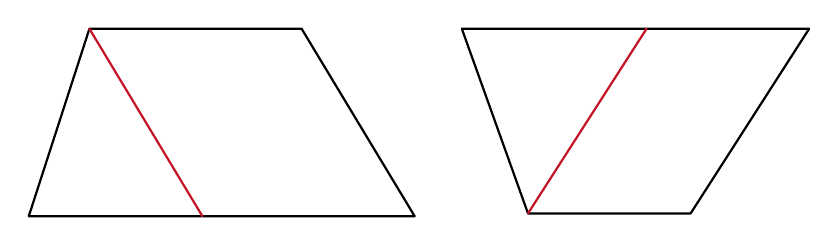
\begin{tikzpicture}[x=.035cm,y=-.035cm,font=\normalsize]
\begin{scope}[shift={(-300,-647)}]
\draw[black,thick] (300,715)--(322,647)--(399,647)--(440,715)--cycle;
\draw[answerred,thick] (322,647)--(363,715);
\end{scope}
\begin{scope}[xshift=5.5cm,shift={(-559,-648)}]
\draw[black,thick] (559,648)--(685,648)--(642,715)--(583,715)--cycle;
\draw[answerred,thick] (583,715)--(626,648);
\end{scope}
\end{tikzpicture}
\end{adjustbox}\par\smallskip
\Answer{新增红色线段各把原梯形分成一个平行四边形和一个三角形。分割线用实线；它们不是作高线。}

\QHeading{第3题②　分成两个全等梯形的另一些画法}

\Answer{经过图形中心，连接一对关于中心相对称的上下底上的点，可以得到两块完全相同的图形；为得到梯形，分割线不能与原来的腰平行。}
\par\smallskip\noindent\begin{adjustbox}{max width=\linewidth,center}
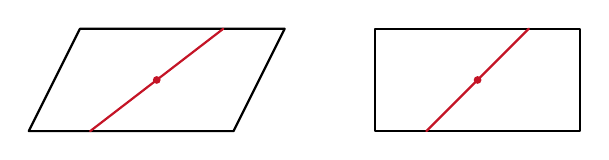
\begin{tikzpicture}[x=.65cm,y=.65cm,font=\normalsize]
\draw[black,thick] (0,0)--(4,0)--(5,2)--(1,2)--cycle;
\draw[answerred,thick] (1.2,0)--(3.8,2);
\fill[answerred] (2.5,1) circle (1.4pt);
\begin{scope}[xshift=4.4cm]
\draw[black,thick] (0,0) rectangle (4,2);
\draw[answerred,thick] (1,0)--(3,2);
\fill[answerred] (2,1) circle (1.4pt);
\end{scope}
\end{tikzpicture}
\end{adjustbox}\par\smallskip
\Answer{两部分可绕中心旋转180度后重合。矩形不能简单从中间画一条竖线来代替本题答案，否则分出的两块都是长方形，不是本题“只有一组对边平行”的梯形。}

\QHeading{第4题　在下面的点子图中分别画一个长方形、一个正方形、一个平行四边形和一个等腰梯形。}

\par\noindent\makebox[\linewidth][c]{
\begin{tikzpicture}[x=1bp,y=-1bp,color=black,draw=black,text=black]
\begin{scope}\clip (70.0,608.0) rectangle (548.0,766.0);
\hdhead{45}{多边形的认识——信息窗3}
\hdsection{1}{132}{填一填。}
\begin{scope}[scale=.6666667,draw=black,text=black]\draw[hdoutline] (382.000,308.000)--(419.000,203.000)--(513.000,203.000)--(550.000,308.000)--cycle;\end{scope}
\begin{scope}[scale=.6666667,draw=black,text=black]\draw[hdoutline,dashed] (419.000,203.000)--(419.000,308.000);\end{scope}
\begin{scope}[scale=.6666667,draw=black,text=black]\draw[line width=.45pt] (419.000,298.000)--(429.000,298.000)--(429.000,308.000);\end{scope}
\q{423}{178}{28}{13}{（}
\q{480}{178}{25}{13}{）}
\q{332}{249}{28}{13}{（}
\q{384}{249}{25}{13}{）}
\q{418}{249}{28}{13}{（}
\q{465}{249}{25}{13}{）}
\q{529}{249}{28}{13}{（}
\q{587}{249}{25}{13}{）}
\q{420}{315}{28}{13}{（}
\q{482}{315}{25}{13}{）}
\hdsection{2}{369}{分别画出下面梯形底边上的高。}
\begin{scope}[scale=.6666667,draw=black,text=black]\draw[hdoutline] (124.000,498.000)--(168.000,428.000)--(261.000,428.000)--(275.000,498.000)--cycle;\end{scope}
\begin{scope}[scale=.6666667,draw=black,text=black]\draw[hdoutline] (356.000,413.000)--(424.000,458.000)--(424.000,520.000)--(356.000,520.000)--cycle;\end{scope}
\begin{scope}[scale=.6666667,draw=black,text=black]\draw[hdoutline] (507.000,447.000)--(634.000,447.000)--(608.000,517.000)--(534.000,517.000)--cycle;\end{scope}
\begin{scope}[scale=.6666667,draw=black,text=black]\draw[hdoutline] (734.000,440.000)--(803.000,440.000)--(803.000,517.000)--(734.000,492.000)--cycle;\end{scope}
\begin{scope}[scale=.6666667,draw=black,text=black]\node[inner sep=0pt,font=\normalsize,text=black] at (201.000,516.000) {底};\end{scope}
\begin{scope}[scale=.6666667,draw=black,text=black]\node[inner sep=0pt,font=\normalsize,text=black] at (344.000,471.000) {底};\end{scope}
\begin{scope}[scale=.6666667,draw=black,text=black]\node[inner sep=0pt,font=\normalsize,text=black] at (571.000,431.000) {底};\end{scope}
\begin{scope}[scale=.6666667,draw=black,text=black]\node[inner sep=0pt,font=\normalsize,text=black] at (722.000,468.000) {底};\end{scope}
\hdsection{3}{559}{画一画，分一分。}
\q{102}{607}{730}{12}{① 在图形中各画一条线段，把图形分成一个平行四边形和一个三角形。}
\begin{scope}[scale=.6666667,draw=black,text=black]\draw[hdoutline] (300.000,715.000)--(322.000,647.000)--(399.000,647.000)--(440.000,715.000)--cycle;\end{scope}
\begin{scope}[scale=.6666667,draw=black,text=black]\draw[hdoutline] (559.000,648.000)--(685.000,648.000)--(642.000,715.000)--(583.000,715.000)--cycle;\end{scope}
\q{103}{738}{734}{12}{② 在每个图形中各画一条线段，把图形分成两个完全相同的梯形。}
\begin{scope}[scale=.6666667,draw=black,text=black]\draw[hdoutline] (301.500,846.000)--(339.500,776.000)--(447.500,776.000)--(409.500,846.000)--cycle;\end{scope}
\begin{scope}[scale=.6666667,draw=black,text=black]\draw[hdoutline] (571.000,776.000)--(680.000,776.000)--(680.000,846.000)--(571.000,846.000)--cycle;\end{scope}
\hdsection{4}{879}{在下面的点子图中分别画一个长方形、一个正方形、一个平行四边形和一个等腰梯形。}
\begin{scope}[scale=.6666667,draw=black,text=black]\foreach \i in {0,...,38}{\foreach \j in {0,...,9}{\fill[black] ({113.6+\i*18.4},{974.2+\j*18.4}) circle (1.15);}}\end{scope}

\begin{scope}[color=answerred,draw=answerred,text=answerred]\ans{296.67}{118.67}{46.67}{10}{上底}
\ans{294.67}{210.00}{46.67}{10}{下底}
\ans{236.00}{166.00}{46.67}{10}{腰}
\ans{367.33}{166.00}{46.67}{10}{腰}
\ans{293.33}{166.00}{46.67}{10}{高}
\draw[answerred,line width=.7pt,dashed] (112.000,285.333) -- (112.000,332.000);
\draw[answerred,line width=.7pt] (117.333,332.000) -- (117.333,326.667);
\draw[answerred,line width=.7pt] (117.333,326.667) -- (112.000,326.667);
\ans{116.00}{303.33}{20.00}{9}{高}
\draw[answerred,line width=.7pt,dashed] (282.667,305.333) -- (237.333,305.333);
\draw[answerred,line width=.7pt] (237.333,310.667) -- (242.667,310.667);
\draw[answerred,line width=.7pt] (242.667,310.667) -- (242.667,305.333);
\ans{264.00}{300.00}{20.00}{9}{高}
\draw[answerred,line width=.7pt,dashed] (356.000,344.667) -- (356.000,298.000);
\draw[answerred,line width=.7pt] (361.333,298.000) -- (361.333,303.333);
\draw[answerred,line width=.7pt] (361.333,303.333) -- (356.000,303.333);
\ans{360.00}{316.00}{20.00}{9}{高}
\draw[answerred,line width=.7pt,dashed] (535.333,306.667) -- (489.333,306.667);
\draw[answerred,line width=.7pt] (489.333,312.000) -- (494.667,312.000);
\draw[answerred,line width=.7pt] (494.667,312.000) -- (494.667,306.667);
\ans{506.67}{309.33}{20.00}{9}{高}
\draw[answerred,line width=.7pt] (266.000,431.333) -- (251.333,476.667);
\draw[answerred,line width=.7pt] (428.000,476.667) -- (412.000,432.000);
\draw[answerred,line width=.7pt] (243.333,517.333) -- (256.000,564.000);
\draw[answerred,line width=.7pt] (400.000,517.333) -- (433.333,564.000);
\draw[answerred,line width=.8pt] (88.000,735.333) -- (174.000,735.333) -- (174.000,674.000) -- (88.000,674.000) -- cycle;
\draw[answerred,line width=.8pt] (211.333,735.333) -- (272.667,735.333) -- (272.667,674.000) -- (211.333,674.000) -- cycle;
\draw[answerred,line width=.8pt] (309.333,735.333) -- (371.333,735.333) -- (396.000,674.000) -- (334.000,674.000) -- cycle;
\draw[answerred,line width=.8pt] (433.333,735.333) -- (532.667,735.333) -- (507.333,686.000) -- (458.667,686.000) -- cycle;
\ans{100.00}{750.67}{100.00}{9}{长方形}
\ans{220.67}{750.67}{100.00}{9}{正方形}
\ans{319.33}{750.67}{100.00}{9}{平行四边形}
\ans{453.33}{750.67}{100.00}{9}{等腰梯形}
\end{scope}
\end{scope}\pgfresetboundingbox\path[use as bounding box] (70.0,608.0) rectangle (548.0,766.0);
\end{tikzpicture}}\par



\par









\QHeading{第2、4题　答案不唯一的范围}

\Answer{梯形的高可以从一条底边上的不同点向另一底边所在直线作出，但必须与两底垂直。长方形、正方形、平行四边形、等腰梯形的自由作图可改变大小和位置；应核对各自的边、角条件，而不能只按本册示例的外观判断。}

\Answer{作高复核：高用虚线，旁边写“高”，垂足处画直角符号；以题目指定的底为准，必要时用虚线延长底边。}

\SourcePage{46}{小数的意义与性质——信息窗1}
\QHeading{第1题　用小数表示下图的涂色部分。}

\par\noindent\makebox[\linewidth][c]{
\begin{tikzpicture}[x=1bp,y=-1bp,color=black,draw=black,text=black]
\begin{scope}\clip (56.0,113.0) rectangle (518.0,261.33);
\hdhead{46}{小数的意义与性质——信息窗1}
\hdsection{1}{135}{用小数表示下图的涂色部分。}
\begin{scope}[scale=.6666667,draw=black,text=black]\path[pattern=north east lines,pattern color=black] (143,178) rectangle (200.6,323);\end{scope}
\begin{scope}[scale=.6666667,draw=black,text=black]\draw[draw=black,line width=.4pt] (143,178) rectangle (287,323);\foreach \i in {1,...,9}{\draw[draw=black,line width=.4pt] ({143+14.4*\i},178)--({143+14.4*\i},323);}\foreach \j in {1,...,0}{\draw[draw=black,line width=.4pt] (143,{178+145.0*\j})--(287,{178+145.0*\j});}\end{scope}
\begin{scope}[scale=.6666667,draw=black,text=black]\path[pattern=north east lines,pattern color=black] (389,178) rectangle (432.2,322);\end{scope}
\begin{scope}[scale=.6666667,draw=black,text=black]\path[pattern=north east lines,pattern color=black] (432.2,278.8) rectangle (446.59999999999997,322.0);\end{scope}
\begin{scope}[scale=.6666667,draw=black,text=black]\draw[draw=black,line width=.35pt] (389,178) rectangle (533,322);\foreach \i in {1,...,9}{\draw[draw=black,line width=.35pt] ({389+14.4*\i},178)--({389+14.4*\i},322);}\foreach \j in {1,...,9}{\draw[draw=black,line width=.35pt] (389,{178+14.4*\j})--(533,{178+14.4*\j});}\end{scope}
\begin{scope}[scale=.6666667,draw=black,text=black]\fill[white] (636.0000,319.0000)--(736.0000,319.0000)--(736.0000,219.0000)--(636.0000,219.0000)--cycle;\end{scope}
\begin{scope}[scale=.6666667,draw=black,text=black]\fill[white] (636.0000,219.0000)--(736.0000,219.0000)--(769.0000,179.0000)--(669.0000,179.0000)--cycle;\end{scope}
\begin{scope}[scale=.6666667,draw=black,text=black]\path[pattern=north east lines,pattern color=black] (736.0000,319.0000)--(769.0000,279.0000)--(769.0000,179.0000)--(736.0000,219.0000)--cycle;\end{scope}
\begin{scope}[scale=.6666667,draw=black,text=black]\path[pattern=north east lines,pattern color=black] (706.0000,249.0000)--(716.0000,249.0000)--(716.0000,239.0000)--(706.0000,239.0000)--cycle;\end{scope}
\begin{scope}[scale=.6666667,draw=black,text=black]\path[pattern=north east lines,pattern color=black] (706.0000,239.0000)--(716.0000,239.0000)--(716.0000,229.0000)--(706.0000,229.0000)--cycle;\end{scope}
\begin{scope}[scale=.6666667,draw=black,text=black]\path[pattern=north east lines,pattern color=black] (706.0000,229.0000)--(716.0000,229.0000)--(716.0000,219.0000)--(706.0000,219.0000)--cycle;\end{scope}
\begin{scope}[scale=.6666667,draw=black,text=black]\path[pattern=north east lines,pattern color=black] (706.0000,219.0000)--(716.0000,219.0000)--(719.3000,215.0000)--(709.3000,215.0000)--cycle;\end{scope}
\begin{scope}[scale=.6666667,draw=black,text=black]\path[pattern=north east lines,pattern color=black] (716.0000,319.0000)--(726.0000,319.0000)--(726.0000,309.0000)--(716.0000,309.0000)--cycle;\end{scope}
\begin{scope}[scale=.6666667,draw=black,text=black]\path[pattern=north east lines,pattern color=black] (716.0000,309.0000)--(726.0000,309.0000)--(726.0000,299.0000)--(716.0000,299.0000)--cycle;\end{scope}
\begin{scope}[scale=.6666667,draw=black,text=black]\path[pattern=north east lines,pattern color=black] (716.0000,299.0000)--(726.0000,299.0000)--(726.0000,289.0000)--(716.0000,289.0000)--cycle;\end{scope}
\begin{scope}[scale=.6666667,draw=black,text=black]\path[pattern=north east lines,pattern color=black] (716.0000,289.0000)--(726.0000,289.0000)--(726.0000,279.0000)--(716.0000,279.0000)--cycle;\end{scope}
\begin{scope}[scale=.6666667,draw=black,text=black]\path[pattern=north east lines,pattern color=black] (716.0000,279.0000)--(726.0000,279.0000)--(726.0000,269.0000)--(716.0000,269.0000)--cycle;\end{scope}
\begin{scope}[scale=.6666667,draw=black,text=black]\path[pattern=north east lines,pattern color=black] (716.0000,269.0000)--(726.0000,269.0000)--(726.0000,259.0000)--(716.0000,259.0000)--cycle;\end{scope}
\begin{scope}[scale=.6666667,draw=black,text=black]\path[pattern=north east lines,pattern color=black] (716.0000,259.0000)--(726.0000,259.0000)--(726.0000,249.0000)--(716.0000,249.0000)--cycle;\end{scope}
\begin{scope}[scale=.6666667,draw=black,text=black]\path[pattern=north east lines,pattern color=black] (716.0000,249.0000)--(726.0000,249.0000)--(726.0000,239.0000)--(716.0000,239.0000)--cycle;\end{scope}
\begin{scope}[scale=.6666667,draw=black,text=black]\path[pattern=north east lines,pattern color=black] (716.0000,239.0000)--(726.0000,239.0000)--(726.0000,229.0000)--(716.0000,229.0000)--cycle;\end{scope}
\begin{scope}[scale=.6666667,draw=black,text=black]\path[pattern=north east lines,pattern color=black] (716.0000,229.0000)--(726.0000,229.0000)--(726.0000,219.0000)--(716.0000,219.0000)--cycle;\end{scope}
\begin{scope}[scale=.6666667,draw=black,text=black]\path[pattern=north east lines,pattern color=black] (716.0000,219.0000)--(726.0000,219.0000)--(729.3000,215.0000)--(719.3000,215.0000)--cycle;\end{scope}
\begin{scope}[scale=.6666667,draw=black,text=black]\path[pattern=north east lines,pattern color=black] (719.3000,215.0000)--(729.3000,215.0000)--(732.6000,211.0000)--(722.6000,211.0000)--cycle;\end{scope}
\begin{scope}[scale=.6666667,draw=black,text=black]\path[pattern=north east lines,pattern color=black] (722.6000,211.0000)--(732.6000,211.0000)--(735.9000,207.0000)--(725.9000,207.0000)--cycle;\end{scope}
\begin{scope}[scale=.6666667,draw=black,text=black]\path[pattern=north east lines,pattern color=black] (725.9000,207.0000)--(735.9000,207.0000)--(739.2000,203.0000)--(729.2000,203.0000)--cycle;\end{scope}
\begin{scope}[scale=.6666667,draw=black,text=black]\path[pattern=north east lines,pattern color=black] (729.2000,203.0000)--(739.2000,203.0000)--(742.5000,199.0000)--(732.5000,199.0000)--cycle;\end{scope}
\begin{scope}[scale=.6666667,draw=black,text=black]\path[pattern=north east lines,pattern color=black] (732.5000,199.0000)--(742.5000,199.0000)--(745.8000,195.0000)--(735.8000,195.0000)--cycle;\end{scope}
\begin{scope}[scale=.6666667,draw=black,text=black]\path[pattern=north east lines,pattern color=black] (735.8000,195.0000)--(745.8000,195.0000)--(749.1000,191.0000)--(739.1000,191.0000)--cycle;\end{scope}
\begin{scope}[scale=.6666667,draw=black,text=black]\path[pattern=north east lines,pattern color=black] (739.1000,191.0000)--(749.1000,191.0000)--(752.4000,187.0000)--(742.4000,187.0000)--cycle;\end{scope}
\begin{scope}[scale=.6666667,draw=black,text=black]\path[pattern=north east lines,pattern color=black] (742.4000,187.0000)--(752.4000,187.0000)--(755.7000,183.0000)--(745.7000,183.0000)--cycle;\end{scope}
\begin{scope}[scale=.6666667,draw=black,text=black]\path[pattern=north east lines,pattern color=black] (745.7000,183.0000)--(755.7000,183.0000)--(759.0000,179.0000)--(749.0000,179.0000)--cycle;\end{scope}
\begin{scope}[scale=.6666667,draw=black,text=black]\path[pattern=north east lines,pattern color=black] (726.0000,319.0000)--(736.0000,319.0000)--(736.0000,309.0000)--(726.0000,309.0000)--cycle;\end{scope}
\begin{scope}[scale=.6666667,draw=black,text=black]\path[pattern=north east lines,pattern color=black] (726.0000,309.0000)--(736.0000,309.0000)--(736.0000,299.0000)--(726.0000,299.0000)--cycle;\end{scope}
\begin{scope}[scale=.6666667,draw=black,text=black]\path[pattern=north east lines,pattern color=black] (726.0000,299.0000)--(736.0000,299.0000)--(736.0000,289.0000)--(726.0000,289.0000)--cycle;\end{scope}
\begin{scope}[scale=.6666667,draw=black,text=black]\path[pattern=north east lines,pattern color=black] (726.0000,289.0000)--(736.0000,289.0000)--(736.0000,279.0000)--(726.0000,279.0000)--cycle;\end{scope}
\begin{scope}[scale=.6666667,draw=black,text=black]\path[pattern=north east lines,pattern color=black] (726.0000,279.0000)--(736.0000,279.0000)--(736.0000,269.0000)--(726.0000,269.0000)--cycle;\end{scope}
\begin{scope}[scale=.6666667,draw=black,text=black]\path[pattern=north east lines,pattern color=black] (726.0000,269.0000)--(736.0000,269.0000)--(736.0000,259.0000)--(726.0000,259.0000)--cycle;\end{scope}
\begin{scope}[scale=.6666667,draw=black,text=black]\path[pattern=north east lines,pattern color=black] (726.0000,259.0000)--(736.0000,259.0000)--(736.0000,249.0000)--(726.0000,249.0000)--cycle;\end{scope}
\begin{scope}[scale=.6666667,draw=black,text=black]\path[pattern=north east lines,pattern color=black] (726.0000,249.0000)--(736.0000,249.0000)--(736.0000,239.0000)--(726.0000,239.0000)--cycle;\end{scope}
\begin{scope}[scale=.6666667,draw=black,text=black]\path[pattern=north east lines,pattern color=black] (726.0000,239.0000)--(736.0000,239.0000)--(736.0000,229.0000)--(726.0000,229.0000)--cycle;\end{scope}
\begin{scope}[scale=.6666667,draw=black,text=black]\path[pattern=north east lines,pattern color=black] (726.0000,229.0000)--(736.0000,229.0000)--(736.0000,219.0000)--(726.0000,219.0000)--cycle;\end{scope}
\begin{scope}[scale=.6666667,draw=black,text=black]\path[pattern=north east lines,pattern color=black] (726.0000,219.0000)--(736.0000,219.0000)--(739.3000,215.0000)--(729.3000,215.0000)--cycle;\end{scope}
\begin{scope}[scale=.6666667,draw=black,text=black]\path[pattern=north east lines,pattern color=black] (729.3000,215.0000)--(739.3000,215.0000)--(742.6000,211.0000)--(732.6000,211.0000)--cycle;\end{scope}
\begin{scope}[scale=.6666667,draw=black,text=black]\path[pattern=north east lines,pattern color=black] (732.6000,211.0000)--(742.6000,211.0000)--(745.9000,207.0000)--(735.9000,207.0000)--cycle;\end{scope}
\begin{scope}[scale=.6666667,draw=black,text=black]\path[pattern=north east lines,pattern color=black] (735.9000,207.0000)--(745.9000,207.0000)--(749.2000,203.0000)--(739.2000,203.0000)--cycle;\end{scope}
\begin{scope}[scale=.6666667,draw=black,text=black]\path[pattern=north east lines,pattern color=black] (739.2000,203.0000)--(749.2000,203.0000)--(752.5000,199.0000)--(742.5000,199.0000)--cycle;\end{scope}
\begin{scope}[scale=.6666667,draw=black,text=black]\path[pattern=north east lines,pattern color=black] (742.5000,199.0000)--(752.5000,199.0000)--(755.8000,195.0000)--(745.8000,195.0000)--cycle;\end{scope}
\begin{scope}[scale=.6666667,draw=black,text=black]\path[pattern=north east lines,pattern color=black] (745.8000,195.0000)--(755.8000,195.0000)--(759.1000,191.0000)--(749.1000,191.0000)--cycle;\end{scope}
\begin{scope}[scale=.6666667,draw=black,text=black]\path[pattern=north east lines,pattern color=black] (749.1000,191.0000)--(759.1000,191.0000)--(762.4000,187.0000)--(752.4000,187.0000)--cycle;\end{scope}
\begin{scope}[scale=.6666667,draw=black,text=black]\path[pattern=north east lines,pattern color=black] (752.4000,187.0000)--(762.4000,187.0000)--(765.7000,183.0000)--(755.7000,183.0000)--cycle;\end{scope}
\begin{scope}[scale=.6666667,draw=black,text=black]\path[pattern=north east lines,pattern color=black] (755.7000,183.0000)--(765.7000,183.0000)--(769.0000,179.0000)--(759.0000,179.0000)--cycle;\end{scope}
\begin{scope}[scale=.6666667,draw=black,text=black]\draw[draw=black!85,line width=.32pt] (636.000,319.000)--(636.000,219.000);\end{scope}
\begin{scope}[scale=.6666667,draw=black,text=black]\draw[draw=black!85,line width=.32pt] (636.000,319.000)--(736.000,319.000);\end{scope}
\begin{scope}[scale=.6666667,draw=black,text=black]\draw[draw=black!85,line width=.32pt] (636.000,219.000)--(669.000,179.000);\end{scope}
\begin{scope}[scale=.6666667,draw=black,text=black]\draw[draw=black!85,line width=.32pt] (636.000,219.000)--(736.000,219.000);\end{scope}
\begin{scope}[scale=.6666667,draw=black,text=black]\draw[draw=black!85,line width=.32pt] (736.000,319.000)--(736.000,219.000);\end{scope}
\begin{scope}[scale=.6666667,draw=black,text=black]\draw[draw=black!85,line width=.32pt] (736.000,319.000)--(769.000,279.000);\end{scope}
\begin{scope}[scale=.6666667,draw=black,text=black]\draw[draw=black!85,line width=.32pt] (646.000,319.000)--(646.000,219.000);\end{scope}
\begin{scope}[scale=.6666667,draw=black,text=black]\draw[draw=black!85,line width=.32pt] (636.000,309.000)--(736.000,309.000);\end{scope}
\begin{scope}[scale=.6666667,draw=black,text=black]\draw[draw=black!85,line width=.32pt] (646.000,219.000)--(679.000,179.000);\end{scope}
\begin{scope}[scale=.6666667,draw=black,text=black]\draw[draw=black!85,line width=.32pt] (639.300,215.000)--(739.300,215.000);\end{scope}
\begin{scope}[scale=.6666667,draw=black,text=black]\draw[draw=black!85,line width=.32pt] (739.300,315.000)--(739.300,215.000);\end{scope}
\begin{scope}[scale=.6666667,draw=black,text=black]\draw[draw=black!85,line width=.32pt] (736.000,309.000)--(769.000,269.000);\end{scope}
\begin{scope}[scale=.6666667,draw=black,text=black]\draw[draw=black!85,line width=.32pt] (656.000,319.000)--(656.000,219.000);\end{scope}
\begin{scope}[scale=.6666667,draw=black,text=black]\draw[draw=black!85,line width=.32pt] (636.000,299.000)--(736.000,299.000);\end{scope}
\begin{scope}[scale=.6666667,draw=black,text=black]\draw[draw=black!85,line width=.32pt] (656.000,219.000)--(689.000,179.000);\end{scope}
\begin{scope}[scale=.6666667,draw=black,text=black]\draw[draw=black!85,line width=.32pt] (642.600,211.000)--(742.600,211.000);\end{scope}
\begin{scope}[scale=.6666667,draw=black,text=black]\draw[draw=black!85,line width=.32pt] (742.600,311.000)--(742.600,211.000);\end{scope}
\begin{scope}[scale=.6666667,draw=black,text=black]\draw[draw=black!85,line width=.32pt] (736.000,299.000)--(769.000,259.000);\end{scope}
\begin{scope}[scale=.6666667,draw=black,text=black]\draw[draw=black!85,line width=.32pt] (666.000,319.000)--(666.000,219.000);\end{scope}
\begin{scope}[scale=.6666667,draw=black,text=black]\draw[draw=black!85,line width=.32pt] (636.000,289.000)--(736.000,289.000);\end{scope}
\begin{scope}[scale=.6666667,draw=black,text=black]\draw[draw=black!85,line width=.32pt] (666.000,219.000)--(699.000,179.000);\end{scope}
\begin{scope}[scale=.6666667,draw=black,text=black]\draw[draw=black!85,line width=.32pt] (645.900,207.000)--(745.900,207.000);\end{scope}
\begin{scope}[scale=.6666667,draw=black,text=black]\draw[draw=black!85,line width=.32pt] (745.900,307.000)--(745.900,207.000);\end{scope}
\begin{scope}[scale=.6666667,draw=black,text=black]\draw[draw=black!85,line width=.32pt] (736.000,289.000)--(769.000,249.000);\end{scope}
\begin{scope}[scale=.6666667,draw=black,text=black]\draw[draw=black!85,line width=.32pt] (676.000,319.000)--(676.000,219.000);\end{scope}
\begin{scope}[scale=.6666667,draw=black,text=black]\draw[draw=black!85,line width=.32pt] (636.000,279.000)--(736.000,279.000);\end{scope}
\begin{scope}[scale=.6666667,draw=black,text=black]\draw[draw=black!85,line width=.32pt] (676.000,219.000)--(709.000,179.000);\end{scope}
\begin{scope}[scale=.6666667,draw=black,text=black]\draw[draw=black!85,line width=.32pt] (649.200,203.000)--(749.200,203.000);\end{scope}
\begin{scope}[scale=.6666667,draw=black,text=black]\draw[draw=black!85,line width=.32pt] (749.200,303.000)--(749.200,203.000);\end{scope}
\begin{scope}[scale=.6666667,draw=black,text=black]\draw[draw=black!85,line width=.32pt] (736.000,279.000)--(769.000,239.000);\end{scope}
\begin{scope}[scale=.6666667,draw=black,text=black]\draw[draw=black!85,line width=.32pt] (686.000,319.000)--(686.000,219.000);\end{scope}
\begin{scope}[scale=.6666667,draw=black,text=black]\draw[draw=black!85,line width=.32pt] (636.000,269.000)--(736.000,269.000);\end{scope}
\begin{scope}[scale=.6666667,draw=black,text=black]\draw[draw=black!85,line width=.32pt] (686.000,219.000)--(719.000,179.000);\end{scope}
\begin{scope}[scale=.6666667,draw=black,text=black]\draw[draw=black!85,line width=.32pt] (652.500,199.000)--(752.500,199.000);\end{scope}
\begin{scope}[scale=.6666667,draw=black,text=black]\draw[draw=black!85,line width=.32pt] (752.500,299.000)--(752.500,199.000);\end{scope}
\begin{scope}[scale=.6666667,draw=black,text=black]\draw[draw=black!85,line width=.32pt] (736.000,269.000)--(769.000,229.000);\end{scope}
\begin{scope}[scale=.6666667,draw=black,text=black]\draw[draw=black!85,line width=.32pt] (696.000,319.000)--(696.000,219.000);\end{scope}
\begin{scope}[scale=.6666667,draw=black,text=black]\draw[draw=black!85,line width=.32pt] (636.000,259.000)--(736.000,259.000);\end{scope}
\begin{scope}[scale=.6666667,draw=black,text=black]\draw[draw=black!85,line width=.32pt] (696.000,219.000)--(729.000,179.000);\end{scope}
\begin{scope}[scale=.6666667,draw=black,text=black]\draw[draw=black!85,line width=.32pt] (655.800,195.000)--(755.800,195.000);\end{scope}
\begin{scope}[scale=.6666667,draw=black,text=black]\draw[draw=black!85,line width=.32pt] (755.800,295.000)--(755.800,195.000);\end{scope}
\begin{scope}[scale=.6666667,draw=black,text=black]\draw[draw=black!85,line width=.32pt] (736.000,259.000)--(769.000,219.000);\end{scope}
\begin{scope}[scale=.6666667,draw=black,text=black]\draw[draw=black!85,line width=.32pt] (706.000,319.000)--(706.000,219.000);\end{scope}
\begin{scope}[scale=.6666667,draw=black,text=black]\draw[draw=black!85,line width=.32pt] (636.000,249.000)--(736.000,249.000);\end{scope}
\begin{scope}[scale=.6666667,draw=black,text=black]\draw[draw=black!85,line width=.32pt] (706.000,219.000)--(739.000,179.000);\end{scope}
\begin{scope}[scale=.6666667,draw=black,text=black]\draw[draw=black!85,line width=.32pt] (659.100,191.000)--(759.100,191.000);\end{scope}
\begin{scope}[scale=.6666667,draw=black,text=black]\draw[draw=black!85,line width=.32pt] (759.100,291.000)--(759.100,191.000);\end{scope}
\begin{scope}[scale=.6666667,draw=black,text=black]\draw[draw=black!85,line width=.32pt] (736.000,249.000)--(769.000,209.000);\end{scope}
\begin{scope}[scale=.6666667,draw=black,text=black]\draw[draw=black!85,line width=.32pt] (716.000,319.000)--(716.000,219.000);\end{scope}
\begin{scope}[scale=.6666667,draw=black,text=black]\draw[draw=black!85,line width=.32pt] (636.000,239.000)--(736.000,239.000);\end{scope}
\begin{scope}[scale=.6666667,draw=black,text=black]\draw[draw=black!85,line width=.32pt] (716.000,219.000)--(749.000,179.000);\end{scope}
\begin{scope}[scale=.6666667,draw=black,text=black]\draw[draw=black!85,line width=.32pt] (662.400,187.000)--(762.400,187.000);\end{scope}
\begin{scope}[scale=.6666667,draw=black,text=black]\draw[draw=black!85,line width=.32pt] (762.400,287.000)--(762.400,187.000);\end{scope}
\begin{scope}[scale=.6666667,draw=black,text=black]\draw[draw=black!85,line width=.32pt] (736.000,239.000)--(769.000,199.000);\end{scope}
\begin{scope}[scale=.6666667,draw=black,text=black]\draw[draw=black!85,line width=.32pt] (726.000,319.000)--(726.000,219.000);\end{scope}
\begin{scope}[scale=.6666667,draw=black,text=black]\draw[draw=black!85,line width=.32pt] (636.000,229.000)--(736.000,229.000);\end{scope}
\begin{scope}[scale=.6666667,draw=black,text=black]\draw[draw=black!85,line width=.32pt] (726.000,219.000)--(759.000,179.000);\end{scope}
\begin{scope}[scale=.6666667,draw=black,text=black]\draw[draw=black!85,line width=.32pt] (665.700,183.000)--(765.700,183.000);\end{scope}
\begin{scope}[scale=.6666667,draw=black,text=black]\draw[draw=black!85,line width=.32pt] (765.700,283.000)--(765.700,183.000);\end{scope}
\begin{scope}[scale=.6666667,draw=black,text=black]\draw[draw=black!85,line width=.32pt] (736.000,229.000)--(769.000,189.000);\end{scope}
\begin{scope}[scale=.6666667,draw=black,text=black]\draw[draw=black!85,line width=.32pt] (736.000,319.000)--(736.000,219.000);\end{scope}
\begin{scope}[scale=.6666667,draw=black,text=black]\draw[draw=black!85,line width=.32pt] (636.000,219.000)--(736.000,219.000);\end{scope}
\begin{scope}[scale=.6666667,draw=black,text=black]\draw[draw=black!85,line width=.32pt] (736.000,219.000)--(769.000,179.000);\end{scope}
\begin{scope}[scale=.6666667,draw=black,text=black]\draw[draw=black!85,line width=.32pt] (669.000,179.000)--(769.000,179.000);\end{scope}
\begin{scope}[scale=.6666667,draw=black,text=black]\draw[draw=black!85,line width=.32pt] (769.000,279.000)--(769.000,179.000);\end{scope}
\begin{scope}[scale=.6666667,draw=black,text=black]\draw[draw=black!85,line width=.32pt] (736.000,219.000)--(769.000,179.000);\end{scope}
\begin{scope}[scale=.6666667,draw=black,text=black]\draw[draw=black,line width=.55pt] (636.000,319.000)--(736.000,319.000)--(736.000,219.000)--(636.000,219.000)--cycle;\end{scope}
\begin{scope}[scale=.6666667,draw=black,text=black]\draw[draw=black,line width=.55pt] (636.000,219.000)--(736.000,219.000)--(769.000,179.000)--(669.000,179.000)--cycle;\end{scope}
\begin{scope}[scale=.6666667,draw=black,text=black]\draw[draw=black,line width=.55pt] (736.000,319.000)--(769.000,279.000)--(769.000,179.000)--(736.000,219.000)--cycle;\end{scope}
\begin{scope}[scale=.6666667,draw=black,text=black]\node[inner sep=0pt,font=\normalsize,text=black] at (123.000,189.000) {①};\end{scope}
\begin{scope}[scale=.6666667,draw=black,text=black]\node[inner sep=0pt,font=\normalsize,text=black] at (370.000,189.000) {②};\end{scope}
\begin{scope}[scale=.6666667,draw=black,text=black]\node[inner sep=0pt,font=\normalsize,text=black] at (617.000,190.000) {③};\end{scope}
\q{171}{339}{28}{13}{（}
\q{247}{339}{25}{13}{）}
\q{418}{339}{28}{13}{（}
\q{493}{339}{25}{13}{）}
\q{657}{338}{28}{13}{（}
\q{733}{338}{25}{13}{）}
\hdsection{2}{395}{给图形涂色表示它下面的小数。}
\begin{scope}[scale=.6666667,draw=black,text=black]\draw[draw=black,line width=.4pt] (143,444) rectangle (287,591);\foreach \i in {1,...,9}{\draw[draw=black,line width=.4pt] ({143+14.4*\i},444)--({143+14.4*\i},591);}\foreach \j in {1,...,0}{\draw[draw=black,line width=.4pt] (143,{444+147.0*\j})--(287,{444+147.0*\j});}\end{scope}
\begin{scope}[scale=.6666667,draw=black,text=black]\draw[draw=black,line width=.35pt] (389,444) rectangle (533,590);\foreach \i in {1,...,9}{\draw[draw=black,line width=.35pt] ({389+14.4*\i},444)--({389+14.4*\i},590);}\foreach \j in {1,...,9}{\draw[draw=black,line width=.35pt] (389,{444+14.6*\j})--(533,{444+14.6*\j});}\end{scope}
\begin{scope}[scale=.6666667,draw=black,text=black]\draw[draw=black,line width=.35pt] (636,444) rectangle (782,590);\foreach \i in {1,...,9}{\draw[draw=black,line width=.35pt] ({636+14.6*\i},444)--({636+14.6*\i},590);}\foreach \j in {1,...,9}{\draw[draw=black,line width=.35pt] (636,{444+14.6*\j})--(782,{444+14.6*\j});}\end{scope}
\begin{scope}[scale=.6666667,draw=black,text=black]\node[inner sep=0pt,font=\normalsize,text=black] at (123.000,451.000) {①};\end{scope}
\begin{scope}[scale=.6666667,draw=black,text=black]\node[inner sep=0pt,font=\normalsize,text=black] at (369.000,451.000) {②};\end{scope}
\begin{scope}[scale=.6666667,draw=black,text=black]\node[inner sep=0pt,font=\normalsize,text=black] at (616.000,451.000) {③};\end{scope}
\begin{scope}[scale=.6666667,draw=black,text=black]\node[inner sep=0pt,font=\normalsize,text=black] at (215.000,612.000) {$0.9$};\end{scope}
\begin{scope}[scale=.6666667,draw=black,text=black]\node[inner sep=0pt,font=\normalsize,text=black] at (461.000,612.000) {$0.09$};\end{scope}
\begin{scope}[scale=.6666667,draw=black,text=black]\node[inner sep=0pt,font=\normalsize,text=black] at (709.000,612.000) {$0.53$};\end{scope}
\hdsection{3}{657}{照样子填一填。}
\begin{scope}[scale=.6666667,draw=black,text=black]\draw[draw=black,line width=.55pt] (210.000,705.000)--(729.000,705.000)--(724.000,721.000)--(733.000,734.000)--(729.000,754.000)--(210.000,754.000)--cycle;\end{scope}
\begin{scope}[scale=.6666667,draw=black,text=black]\draw[draw=black,line width=.35pt] (219.000,705.000)--(219.000,719.000);\end{scope}
\begin{scope}[scale=.6666667,draw=black,text=black]\draw[draw=black,line width=.35pt] (223.767,705.000)--(223.767,711.000);\end{scope}
\begin{scope}[scale=.6666667,draw=black,text=black]\draw[draw=black,line width=.35pt] (228.533,705.000)--(228.533,711.000);\end{scope}
\begin{scope}[scale=.6666667,draw=black,text=black]\draw[draw=black,line width=.35pt] (233.300,705.000)--(233.300,711.000);\end{scope}
\begin{scope}[scale=.6666667,draw=black,text=black]\draw[draw=black,line width=.35pt] (238.067,705.000)--(238.067,711.000);\end{scope}
\begin{scope}[scale=.6666667,draw=black,text=black]\draw[draw=black,line width=.35pt] (242.833,705.000)--(242.833,714.000);\end{scope}
\begin{scope}[scale=.6666667,draw=black,text=black]\draw[draw=black,line width=.35pt] (247.600,705.000)--(247.600,711.000);\end{scope}
\begin{scope}[scale=.6666667,draw=black,text=black]\draw[draw=black,line width=.35pt] (252.367,705.000)--(252.367,711.000);\end{scope}
\begin{scope}[scale=.6666667,draw=black,text=black]\draw[draw=black,line width=.35pt] (257.133,705.000)--(257.133,711.000);\end{scope}
\begin{scope}[scale=.6666667,draw=black,text=black]\draw[draw=black,line width=.35pt] (261.900,705.000)--(261.900,711.000);\end{scope}
\begin{scope}[scale=.6666667,draw=black,text=black]\draw[draw=black,line width=.35pt] (266.667,705.000)--(266.667,719.000);\end{scope}
\begin{scope}[scale=.6666667,draw=black,text=black]\draw[draw=black,line width=.35pt] (271.433,705.000)--(271.433,711.000);\end{scope}
\begin{scope}[scale=.6666667,draw=black,text=black]\draw[draw=black,line width=.35pt] (276.200,705.000)--(276.200,711.000);\end{scope}
\begin{scope}[scale=.6666667,draw=black,text=black]\draw[draw=black,line width=.35pt] (280.967,705.000)--(280.967,711.000);\end{scope}
\begin{scope}[scale=.6666667,draw=black,text=black]\draw[draw=black,line width=.35pt] (285.733,705.000)--(285.733,711.000);\end{scope}
\begin{scope}[scale=.6666667,draw=black,text=black]\draw[draw=black,line width=.35pt] (290.500,705.000)--(290.500,714.000);\end{scope}
\begin{scope}[scale=.6666667,draw=black,text=black]\draw[draw=black,line width=.35pt] (295.267,705.000)--(295.267,711.000);\end{scope}
\begin{scope}[scale=.6666667,draw=black,text=black]\draw[draw=black,line width=.35pt] (300.033,705.000)--(300.033,711.000);\end{scope}
\begin{scope}[scale=.6666667,draw=black,text=black]\draw[draw=black,line width=.35pt] (304.800,705.000)--(304.800,711.000);\end{scope}
\begin{scope}[scale=.6666667,draw=black,text=black]\draw[draw=black,line width=.35pt] (309.567,705.000)--(309.567,711.000);\end{scope}
\begin{scope}[scale=.6666667,draw=black,text=black]\draw[draw=black,line width=.35pt] (314.333,705.000)--(314.333,719.000);\end{scope}
\begin{scope}[scale=.6666667,draw=black,text=black]\draw[draw=black,line width=.35pt] (319.100,705.000)--(319.100,711.000);\end{scope}
\begin{scope}[scale=.6666667,draw=black,text=black]\draw[draw=black,line width=.35pt] (323.867,705.000)--(323.867,711.000);\end{scope}
\begin{scope}[scale=.6666667,draw=black,text=black]\draw[draw=black,line width=.35pt] (328.633,705.000)--(328.633,711.000);\end{scope}
\begin{scope}[scale=.6666667,draw=black,text=black]\draw[draw=black,line width=.35pt] (333.400,705.000)--(333.400,711.000);\end{scope}
\begin{scope}[scale=.6666667,draw=black,text=black]\draw[draw=black,line width=.35pt] (338.167,705.000)--(338.167,714.000);\end{scope}
\begin{scope}[scale=.6666667,draw=black,text=black]\draw[draw=black,line width=.35pt] (342.933,705.000)--(342.933,711.000);\end{scope}
\begin{scope}[scale=.6666667,draw=black,text=black]\draw[draw=black,line width=.35pt] (347.700,705.000)--(347.700,711.000);\end{scope}
\begin{scope}[scale=.6666667,draw=black,text=black]\draw[draw=black,line width=.35pt] (352.467,705.000)--(352.467,711.000);\end{scope}
\begin{scope}[scale=.6666667,draw=black,text=black]\draw[draw=black,line width=.35pt] (357.233,705.000)--(357.233,711.000);\end{scope}
\begin{scope}[scale=.6666667,draw=black,text=black]\draw[draw=black,line width=.35pt] (362.000,705.000)--(362.000,719.000);\end{scope}
\begin{scope}[scale=.6666667,draw=black,text=black]\draw[draw=black,line width=.35pt] (366.767,705.000)--(366.767,711.000);\end{scope}
\begin{scope}[scale=.6666667,draw=black,text=black]\draw[draw=black,line width=.35pt] (371.533,705.000)--(371.533,711.000);\end{scope}
\begin{scope}[scale=.6666667,draw=black,text=black]\draw[draw=black,line width=.35pt] (376.300,705.000)--(376.300,711.000);\end{scope}
\begin{scope}[scale=.6666667,draw=black,text=black]\draw[draw=black,line width=.35pt] (381.067,705.000)--(381.067,711.000);\end{scope}
\begin{scope}[scale=.6666667,draw=black,text=black]\draw[draw=black,line width=.35pt] (385.833,705.000)--(385.833,714.000);\end{scope}
\begin{scope}[scale=.6666667,draw=black,text=black]\draw[draw=black,line width=.35pt] (390.600,705.000)--(390.600,711.000);\end{scope}
\begin{scope}[scale=.6666667,draw=black,text=black]\draw[draw=black,line width=.35pt] (395.367,705.000)--(395.367,711.000);\end{scope}
\begin{scope}[scale=.6666667,draw=black,text=black]\draw[draw=black,line width=.35pt] (400.133,705.000)--(400.133,711.000);\end{scope}
\begin{scope}[scale=.6666667,draw=black,text=black]\draw[draw=black,line width=.35pt] (404.900,705.000)--(404.900,711.000);\end{scope}
\begin{scope}[scale=.6666667,draw=black,text=black]\draw[draw=black,line width=.35pt] (409.667,705.000)--(409.667,719.000);\end{scope}
\begin{scope}[scale=.6666667,draw=black,text=black]\draw[draw=black,line width=.35pt] (414.433,705.000)--(414.433,711.000);\end{scope}
\begin{scope}[scale=.6666667,draw=black,text=black]\draw[draw=black,line width=.35pt] (419.200,705.000)--(419.200,711.000);\end{scope}
\begin{scope}[scale=.6666667,draw=black,text=black]\draw[draw=black,line width=.35pt] (423.967,705.000)--(423.967,711.000);\end{scope}
\begin{scope}[scale=.6666667,draw=black,text=black]\draw[draw=black,line width=.35pt] (428.733,705.000)--(428.733,711.000);\end{scope}
\begin{scope}[scale=.6666667,draw=black,text=black]\draw[draw=black,line width=.35pt] (433.500,705.000)--(433.500,714.000);\end{scope}
\begin{scope}[scale=.6666667,draw=black,text=black]\draw[draw=black,line width=.35pt] (438.267,705.000)--(438.267,711.000);\end{scope}
\begin{scope}[scale=.6666667,draw=black,text=black]\draw[draw=black,line width=.35pt] (443.033,705.000)--(443.033,711.000);\end{scope}
\begin{scope}[scale=.6666667,draw=black,text=black]\draw[draw=black,line width=.35pt] (447.800,705.000)--(447.800,711.000);\end{scope}
\begin{scope}[scale=.6666667,draw=black,text=black]\draw[draw=black,line width=.35pt] (452.567,705.000)--(452.567,711.000);\end{scope}
\begin{scope}[scale=.6666667,draw=black,text=black]\draw[draw=black,line width=.35pt] (457.333,705.000)--(457.333,719.000);\end{scope}
\begin{scope}[scale=.6666667,draw=black,text=black]\draw[draw=black,line width=.35pt] (462.100,705.000)--(462.100,711.000);\end{scope}
\begin{scope}[scale=.6666667,draw=black,text=black]\draw[draw=black,line width=.35pt] (466.867,705.000)--(466.867,711.000);\end{scope}
\begin{scope}[scale=.6666667,draw=black,text=black]\draw[draw=black,line width=.35pt] (471.633,705.000)--(471.633,711.000);\end{scope}
\begin{scope}[scale=.6666667,draw=black,text=black]\draw[draw=black,line width=.35pt] (476.400,705.000)--(476.400,711.000);\end{scope}
\begin{scope}[scale=.6666667,draw=black,text=black]\draw[draw=black,line width=.35pt] (481.167,705.000)--(481.167,714.000);\end{scope}
\begin{scope}[scale=.6666667,draw=black,text=black]\draw[draw=black,line width=.35pt] (485.933,705.000)--(485.933,711.000);\end{scope}
\begin{scope}[scale=.6666667,draw=black,text=black]\draw[draw=black,line width=.35pt] (490.700,705.000)--(490.700,711.000);\end{scope}
\begin{scope}[scale=.6666667,draw=black,text=black]\draw[draw=black,line width=.35pt] (495.467,705.000)--(495.467,711.000);\end{scope}
\begin{scope}[scale=.6666667,draw=black,text=black]\draw[draw=black,line width=.35pt] (500.233,705.000)--(500.233,711.000);\end{scope}
\begin{scope}[scale=.6666667,draw=black,text=black]\draw[draw=black,line width=.35pt] (505.000,705.000)--(505.000,719.000);\end{scope}
\begin{scope}[scale=.6666667,draw=black,text=black]\draw[draw=black,line width=.35pt] (509.767,705.000)--(509.767,711.000);\end{scope}
\begin{scope}[scale=.6666667,draw=black,text=black]\draw[draw=black,line width=.35pt] (514.533,705.000)--(514.533,711.000);\end{scope}
\begin{scope}[scale=.6666667,draw=black,text=black]\draw[draw=black,line width=.35pt] (519.300,705.000)--(519.300,711.000);\end{scope}
\begin{scope}[scale=.6666667,draw=black,text=black]\draw[draw=black,line width=.35pt] (524.067,705.000)--(524.067,711.000);\end{scope}
\begin{scope}[scale=.6666667,draw=black,text=black]\draw[draw=black,line width=.35pt] (528.833,705.000)--(528.833,714.000);\end{scope}
\begin{scope}[scale=.6666667,draw=black,text=black]\draw[draw=black,line width=.35pt] (533.600,705.000)--(533.600,711.000);\end{scope}
\begin{scope}[scale=.6666667,draw=black,text=black]\draw[draw=black,line width=.35pt] (538.367,705.000)--(538.367,711.000);\end{scope}
\begin{scope}[scale=.6666667,draw=black,text=black]\draw[draw=black,line width=.35pt] (543.133,705.000)--(543.133,711.000);\end{scope}
\begin{scope}[scale=.6666667,draw=black,text=black]\draw[draw=black,line width=.35pt] (547.900,705.000)--(547.900,711.000);\end{scope}
\begin{scope}[scale=.6666667,draw=black,text=black]\draw[draw=black,line width=.35pt] (552.667,705.000)--(552.667,719.000);\end{scope}
\begin{scope}[scale=.6666667,draw=black,text=black]\draw[draw=black,line width=.35pt] (557.433,705.000)--(557.433,711.000);\end{scope}
\begin{scope}[scale=.6666667,draw=black,text=black]\draw[draw=black,line width=.35pt] (562.200,705.000)--(562.200,711.000);\end{scope}
\begin{scope}[scale=.6666667,draw=black,text=black]\draw[draw=black,line width=.35pt] (566.967,705.000)--(566.967,711.000);\end{scope}
\begin{scope}[scale=.6666667,draw=black,text=black]\draw[draw=black,line width=.35pt] (571.733,705.000)--(571.733,711.000);\end{scope}
\begin{scope}[scale=.6666667,draw=black,text=black]\draw[draw=black,line width=.35pt] (576.500,705.000)--(576.500,714.000);\end{scope}
\begin{scope}[scale=.6666667,draw=black,text=black]\draw[draw=black,line width=.35pt] (581.267,705.000)--(581.267,711.000);\end{scope}
\begin{scope}[scale=.6666667,draw=black,text=black]\draw[draw=black,line width=.35pt] (586.033,705.000)--(586.033,711.000);\end{scope}
\begin{scope}[scale=.6666667,draw=black,text=black]\draw[draw=black,line width=.35pt] (590.800,705.000)--(590.800,711.000);\end{scope}
\begin{scope}[scale=.6666667,draw=black,text=black]\draw[draw=black,line width=.35pt] (595.567,705.000)--(595.567,711.000);\end{scope}
\begin{scope}[scale=.6666667,draw=black,text=black]\draw[draw=black,line width=.35pt] (600.333,705.000)--(600.333,719.000);\end{scope}
\begin{scope}[scale=.6666667,draw=black,text=black]\draw[draw=black,line width=.35pt] (605.100,705.000)--(605.100,711.000);\end{scope}
\begin{scope}[scale=.6666667,draw=black,text=black]\draw[draw=black,line width=.35pt] (609.867,705.000)--(609.867,711.000);\end{scope}
\begin{scope}[scale=.6666667,draw=black,text=black]\draw[draw=black,line width=.35pt] (614.633,705.000)--(614.633,711.000);\end{scope}
\begin{scope}[scale=.6666667,draw=black,text=black]\draw[draw=black,line width=.35pt] (619.400,705.000)--(619.400,711.000);\end{scope}
\begin{scope}[scale=.6666667,draw=black,text=black]\draw[draw=black,line width=.35pt] (624.167,705.000)--(624.167,714.000);\end{scope}
\begin{scope}[scale=.6666667,draw=black,text=black]\draw[draw=black,line width=.35pt] (628.933,705.000)--(628.933,711.000);\end{scope}
\begin{scope}[scale=.6666667,draw=black,text=black]\draw[draw=black,line width=.35pt] (633.700,705.000)--(633.700,711.000);\end{scope}
\begin{scope}[scale=.6666667,draw=black,text=black]\draw[draw=black,line width=.35pt] (638.467,705.000)--(638.467,711.000);\end{scope}
\begin{scope}[scale=.6666667,draw=black,text=black]\draw[draw=black,line width=.35pt] (643.233,705.000)--(643.233,711.000);\end{scope}
\begin{scope}[scale=.6666667,draw=black,text=black]\draw[draw=black,line width=.35pt] (648.000,705.000)--(648.000,719.000);\end{scope}
\begin{scope}[scale=.6666667,draw=black,text=black]\draw[draw=black,line width=.35pt] (652.767,705.000)--(652.767,711.000);\end{scope}
\begin{scope}[scale=.6666667,draw=black,text=black]\draw[draw=black,line width=.35pt] (657.533,705.000)--(657.533,711.000);\end{scope}
\begin{scope}[scale=.6666667,draw=black,text=black]\draw[draw=black,line width=.35pt] (662.300,705.000)--(662.300,711.000);\end{scope}
\begin{scope}[scale=.6666667,draw=black,text=black]\draw[draw=black,line width=.35pt] (667.067,705.000)--(667.067,711.000);\end{scope}
\begin{scope}[scale=.6666667,draw=black,text=black]\draw[draw=black,line width=.35pt] (671.833,705.000)--(671.833,714.000);\end{scope}
\begin{scope}[scale=.6666667,draw=black,text=black]\draw[draw=black,line width=.35pt] (676.600,705.000)--(676.600,711.000);\end{scope}
\begin{scope}[scale=.6666667,draw=black,text=black]\draw[draw=black,line width=.35pt] (681.367,705.000)--(681.367,711.000);\end{scope}
\begin{scope}[scale=.6666667,draw=black,text=black]\draw[draw=black,line width=.35pt] (686.133,705.000)--(686.133,711.000);\end{scope}
\begin{scope}[scale=.6666667,draw=black,text=black]\draw[draw=black,line width=.35pt] (690.900,705.000)--(690.900,711.000);\end{scope}
\begin{scope}[scale=.6666667,draw=black,text=black]\draw[draw=black,line width=.35pt] (695.667,705.000)--(695.667,719.000);\end{scope}
\begin{scope}[scale=.6666667,draw=black,text=black]\node[inner sep=0pt,font=\normalsize,text=black] at (219.000,738.000) {0};\end{scope}
\begin{scope}[scale=.6666667,draw=black,text=black]\node[inner sep=0pt,font=\normalsize,text=black] at (266.667,738.000) {1 cm};\end{scope}
\begin{scope}[scale=.6666667,draw=black,text=black]\node[inner sep=0pt,font=\normalsize,text=black] at (314.333,738.000) {2};\end{scope}
\begin{scope}[scale=.6666667,draw=black,text=black]\node[inner sep=0pt,font=\normalsize,text=black] at (362.000,738.000) {3};\end{scope}
\begin{scope}[scale=.6666667,draw=black,text=black]\node[inner sep=0pt,font=\normalsize,text=black] at (409.667,738.000) {4};\end{scope}
\begin{scope}[scale=.6666667,draw=black,text=black]\node[inner sep=0pt,font=\normalsize,text=black] at (457.333,738.000) {5};\end{scope}
\begin{scope}[scale=.6666667,draw=black,text=black]\node[inner sep=0pt,font=\normalsize,text=black] at (505.000,738.000) {6};\end{scope}
\begin{scope}[scale=.6666667,draw=black,text=black]\node[inner sep=0pt,font=\normalsize,text=black] at (552.667,738.000) {7};\end{scope}
\begin{scope}[scale=.6666667,draw=black,text=black]\node[inner sep=0pt,font=\normalsize,text=black] at (600.333,738.000) {8};\end{scope}
\begin{scope}[scale=.6666667,draw=black,text=black]\node[inner sep=0pt,font=\normalsize,text=black] at (648.000,738.000) {9};\end{scope}
\begin{scope}[scale=.6666667,draw=black,text=black]\node[inner sep=0pt,font=\normalsize,text=black] at (695.667,738.000) {10};\end{scope}
\begin{scope}[scale=.6666667,draw=black,text=black]\draw[draw=black,line width=.45pt,-{Stealth[length=3pt,width=2.4pt]}] (267.000,760.000)--(267.000,785.000);\end{scope}
\begin{scope}[scale=.6666667,draw=black,text=black]\draw[draw=black,line width=.45pt,-{Stealth[length=3pt,width=2.4pt]}] (362.000,760.000)--(362.000,785.000);\end{scope}
\begin{scope}[scale=.6666667,draw=black,text=black]\draw[draw=black,line width=.45pt,-{Stealth[length=3pt,width=2.4pt]}] (505.000,760.000)--(505.000,785.000);\end{scope}
\q{230}{790}{85}{12.5}{$\dfrac1{10}$分米}
\q{331}{790}{96}{12.5}{$\dfrac3{10}$分米}
\q{463}{804}{28}{13}{（}
\q{512}{804}{25}{13}{）}
\q{533}{804}{80}{12.5}{分米}
\q{225}{862}{103}{12.5}{0.1分米}
\q{324}{861}{28}{13}{（}
\q{378}{861}{25}{13}{）}
\q{399}{861}{76}{12.5}{分米}
\q{463}{861}{28}{13}{（}
\q{514}{861}{25}{13}{）}
\q{535}{861}{75}{12.5}{分米}
\hdsection{4}{921}{在计数器上表示下面各小数。}
\q{112}{967}{172}{13}{① 0.35}
\q{368}{967}{172}{13}{② 4.3}
\q{623}{967}{172}{13}{③ 0.732}
\begin{scope}[scale=.6666667,draw=black,text=black]\draw[line width=.5pt] (143,1015) rectangle (287,1079);\draw[line width=.5pt] (143,1019)--(287,1019);\end{scope}
\begin{scope}[scale=.6666667,draw=black,text=black]\draw[line width=.45pt] (165,1017)--(165,1079);\draw[line width=.45pt] (157,1015)..controls(166,995) and (171,1003)..(170,1015);\end{scope}
\begin{scope}[scale=.6666667,draw=black,text=black]\draw[line width=.45pt] (191,1017)--(191,1079);\draw[line width=.45pt] (183,1015)..controls(192,995) and (197,1003)..(196,1015);\end{scope}
\begin{scope}[scale=.6666667,draw=black,text=black]\draw[line width=.45pt] (224,1017)--(224,1079);\draw[line width=.45pt] (216,1015)..controls(225,995) and (230,1003)..(229,1015);\end{scope}
\begin{scope}[scale=.6666667,draw=black,text=black]\draw[line width=.45pt] (247,1017)--(247,1079);\draw[line width=.45pt] (239,1015)..controls(248,995) and (253,1003)..(252,1015);\end{scope}
\begin{scope}[scale=.6666667,draw=black,text=black]\draw[line width=.45pt] (273,1017)--(273,1079);\draw[line width=.45pt] (265,1015)..controls(274,995) and (279,1003)..(278,1015);\end{scope}
\begin{scope}[scale=.6666667,draw=black,text=black]\draw[draw=black,line width=.5pt,fill=white] (143.000,1078.000)--(151.000,1083.000)--(294.000,1083.000)--(287.000,1078.000)--cycle;\end{scope}
\begin{scope}[scale=.6666667,draw=black,text=black]\draw[draw=black,line width=.5pt,fill=white] (151.000,1083.000)--(294.000,1083.000)--(294.000,1147.000)--(151.000,1147.000)--cycle;\end{scope}
\begin{scope}[scale=.6666667,draw=black,text=black]\draw[draw=black,line width=.5pt,fill=white] (143.000,1078.000)--(151.000,1083.000)--(151.000,1147.000)--(143.000,1131.000)--cycle;\end{scope}
\begin{scope}[scale=.6666667,draw=black,text=black]\node[inner sep=0pt,font=\normalsize,text=black] at (165.000,1115.000) {\shortstack{十\\位}};\end{scope}
\begin{scope}[scale=.6666667,draw=black,text=black]\node[inner sep=0pt,font=\normalsize,text=black] at (191.000,1115.000) {\shortstack{个\\位}};\end{scope}
\begin{scope}[scale=.6666667,draw=black,text=black]\node[inner sep=0pt,font=\normalsize,text=black] at (224.000,1115.000) {\shortstack{十\\分\\位}};\end{scope}
\begin{scope}[scale=.6666667,draw=black,text=black]\node[inner sep=0pt,font=\normalsize,text=black] at (247.000,1115.000) {\shortstack{百\\分\\位}};\end{scope}
\begin{scope}[scale=.6666667,draw=black,text=black]\node[inner sep=0pt,font=\normalsize,text=black] at (273.000,1115.000) {\shortstack{千\\分\\位}};\end{scope}
\begin{scope}[scale=.6666667,draw=black,text=black]\draw[line width=.5pt] (398,1015) rectangle (542,1079);\draw[line width=.5pt] (398,1019)--(542,1019);\end{scope}
\begin{scope}[scale=.6666667,draw=black,text=black]\draw[line width=.45pt] (416,1017)--(416,1079);\draw[line width=.45pt] (408,1015)..controls(417,995) and (422,1003)..(421,1015);\end{scope}
\begin{scope}[scale=.6666667,draw=black,text=black]\draw[line width=.45pt] (441,1017)--(441,1079);\draw[line width=.45pt] (433,1015)..controls(442,995) and (447,1003)..(446,1015);\end{scope}
\begin{scope}[scale=.6666667,draw=black,text=black]\draw[line width=.45pt] (477,1017)--(477,1079);\draw[line width=.45pt] (469,1015)..controls(478,995) and (483,1003)..(482,1015);\end{scope}
\begin{scope}[scale=.6666667,draw=black,text=black]\draw[line width=.45pt] (502,1017)--(502,1079);\draw[line width=.45pt] (494,1015)..controls(503,995) and (508,1003)..(507,1015);\end{scope}
\begin{scope}[scale=.6666667,draw=black,text=black]\draw[line width=.45pt] (527,1017)--(527,1079);\draw[line width=.45pt] (519,1015)..controls(528,995) and (533,1003)..(532,1015);\end{scope}
\begin{scope}[scale=.6666667,draw=black,text=black]\draw[draw=black,line width=.5pt,fill=white] (398.000,1078.000)--(406.000,1083.000)--(549.000,1083.000)--(542.000,1078.000)--cycle;\end{scope}
\begin{scope}[scale=.6666667,draw=black,text=black]\draw[draw=black,line width=.5pt,fill=white] (406.000,1083.000)--(549.000,1083.000)--(549.000,1147.000)--(406.000,1147.000)--cycle;\end{scope}
\begin{scope}[scale=.6666667,draw=black,text=black]\draw[draw=black,line width=.5pt,fill=white] (398.000,1078.000)--(406.000,1083.000)--(406.000,1147.000)--(398.000,1131.000)--cycle;\end{scope}
\begin{scope}[scale=.6666667,draw=black,text=black]\node[inner sep=0pt,font=\normalsize,text=black] at (416.000,1115.000) {\shortstack{十\\位}};\end{scope}
\begin{scope}[scale=.6666667,draw=black,text=black]\node[inner sep=0pt,font=\normalsize,text=black] at (441.000,1115.000) {\shortstack{个\\位}};\end{scope}
\begin{scope}[scale=.6666667,draw=black,text=black]\node[inner sep=0pt,font=\normalsize,text=black] at (477.000,1115.000) {\shortstack{十\\分\\位}};\end{scope}
\begin{scope}[scale=.6666667,draw=black,text=black]\node[inner sep=0pt,font=\normalsize,text=black] at (502.000,1115.000) {\shortstack{百\\分\\位}};\end{scope}
\begin{scope}[scale=.6666667,draw=black,text=black]\node[inner sep=0pt,font=\normalsize,text=black] at (527.000,1115.000) {\shortstack{千\\分\\位}};\end{scope}
\begin{scope}[scale=.6666667,draw=black,text=black]\draw[line width=.5pt] (654,1015) rectangle (798,1079);\draw[line width=.5pt] (654,1019)--(798,1019);\end{scope}
\begin{scope}[scale=.6666667,draw=black,text=black]\draw[line width=.45pt] (675,1017)--(675,1079);\draw[line width=.45pt] (667,1015)..controls(676,995) and (681,1003)..(680,1015);\end{scope}
\begin{scope}[scale=.6666667,draw=black,text=black]\draw[line width=.45pt] (701,1017)--(701,1079);\draw[line width=.45pt] (693,1015)..controls(702,995) and (707,1003)..(706,1015);\end{scope}
\begin{scope}[scale=.6666667,draw=black,text=black]\draw[line width=.45pt] (731,1017)--(731,1079);\draw[line width=.45pt] (723,1015)..controls(732,995) and (737,1003)..(736,1015);\end{scope}
\begin{scope}[scale=.6666667,draw=black,text=black]\draw[line width=.45pt] (757,1017)--(757,1079);\draw[line width=.45pt] (749,1015)..controls(758,995) and (763,1003)..(762,1015);\end{scope}
\begin{scope}[scale=.6666667,draw=black,text=black]\draw[line width=.45pt] (781,1017)--(781,1079);\draw[line width=.45pt] (773,1015)..controls(782,995) and (787,1003)..(786,1015);\end{scope}
\begin{scope}[scale=.6666667,draw=black,text=black]\draw[draw=black,line width=.5pt,fill=white] (654.000,1078.000)--(662.000,1083.000)--(805.000,1083.000)--(798.000,1078.000)--cycle;\end{scope}
\begin{scope}[scale=.6666667,draw=black,text=black]\draw[draw=black,line width=.5pt,fill=white] (662.000,1083.000)--(805.000,1083.000)--(805.000,1147.000)--(662.000,1147.000)--cycle;\end{scope}
\begin{scope}[scale=.6666667,draw=black,text=black]\draw[draw=black,line width=.5pt,fill=white] (654.000,1078.000)--(662.000,1083.000)--(662.000,1147.000)--(654.000,1131.000)--cycle;\end{scope}
\begin{scope}[scale=.6666667,draw=black,text=black]\node[inner sep=0pt,font=\normalsize,text=black] at (675.000,1115.000) {\shortstack{十\\位}};\end{scope}
\begin{scope}[scale=.6666667,draw=black,text=black]\node[inner sep=0pt,font=\normalsize,text=black] at (701.000,1115.000) {\shortstack{个\\位}};\end{scope}
\begin{scope}[scale=.6666667,draw=black,text=black]\node[inner sep=0pt,font=\normalsize,text=black] at (731.000,1115.000) {\shortstack{十\\分\\位}};\end{scope}
\begin{scope}[scale=.6666667,draw=black,text=black]\node[inner sep=0pt,font=\normalsize,text=black] at (757.000,1115.000) {\shortstack{百\\分\\位}};\end{scope}
\begin{scope}[scale=.6666667,draw=black,text=black]\node[inner sep=0pt,font=\normalsize,text=black] at (781.000,1115.000) {\shortstack{千\\分\\位}};\end{scope}

\begin{scope}[color=answerred,draw=answerred,text=answerred]\ans{128.00}{226.67}{33.33}{10}{$\vphantom{0}0.4$}
\ans{294.00}{226.67}{33.33}{10}{$\vphantom{0}0.33$}
\ans{455.33}{225.33}{33.33}{10}{$\vphantom{0}0.203$}
\fill[answerred,opacity=.28](95.333,296.000) rectangle (181.733,394.000);
\fill[answerred,opacity=.28](259.333,296.000) rectangle (345.733,305.733);
\fill[answerred,opacity=.28](424.000,296.000) rectangle (472.667,393.333);
\fill[answerred,opacity=.28](472.667,296.000) rectangle (482.400,325.200);
\ans{228.67}{573.33}{48.00}{11}{$\vphantom{0}0.3$}
\ans{322.67}{534.00}{42.00}{11}{$\vphantom{0}\frac6{10}$}
\ans{321.33}{573.33}{48.00}{11}{$\vphantom{0}0.6$}
\filldraw[answerred,fill=answerred!65] (149.333,714.000) ellipse [x radius=4bp,y radius=2.2bp];
\filldraw[answerred,fill=answerred!65] (149.333,708.667) ellipse [x radius=4bp,y radius=2.2bp];
\filldraw[answerred,fill=answerred!65] (149.333,703.333) ellipse [x radius=4bp,y radius=2.2bp];
\filldraw[answerred,fill=answerred!65] (164.667,714.000) ellipse [x radius=4bp,y radius=2.2bp];
\filldraw[answerred,fill=answerred!65] (164.667,708.667) ellipse [x radius=4bp,y radius=2.2bp];
\filldraw[answerred,fill=answerred!65] (164.667,703.333) ellipse [x radius=4bp,y radius=2.2bp];
\filldraw[answerred,fill=answerred!65] (164.667,698.000) ellipse [x radius=4bp,y radius=2.2bp];
\filldraw[answerred,fill=answerred!65] (164.667,692.667) ellipse [x radius=4bp,y radius=2.2bp];
\filldraw[answerred,fill=answerred!65] (294.000,714.000) ellipse [x radius=4bp,y radius=2.2bp];
\filldraw[answerred,fill=answerred!65] (294.000,708.667) ellipse [x radius=4bp,y radius=2.2bp];
\filldraw[answerred,fill=answerred!65] (294.000,703.333) ellipse [x radius=4bp,y radius=2.2bp];
\filldraw[answerred,fill=answerred!65] (294.000,698.000) ellipse [x radius=4bp,y radius=2.2bp];
\filldraw[answerred,fill=answerred!65] (318.000,714.000) ellipse [x radius=4bp,y radius=2.2bp];
\filldraw[answerred,fill=answerred!65] (318.000,708.667) ellipse [x radius=4bp,y radius=2.2bp];
\filldraw[answerred,fill=answerred!65] (318.000,703.333) ellipse [x radius=4bp,y radius=2.2bp];
\filldraw[answerred,fill=answerred!65] (487.333,714.000) ellipse [x radius=4bp,y radius=2.2bp];
\filldraw[answerred,fill=answerred!65] (487.333,708.667) ellipse [x radius=4bp,y radius=2.2bp];
\filldraw[answerred,fill=answerred!65] (487.333,703.333) ellipse [x radius=4bp,y radius=2.2bp];
\filldraw[answerred,fill=answerred!65] (487.333,698.000) ellipse [x radius=4bp,y radius=2.2bp];
\filldraw[answerred,fill=answerred!65] (487.333,692.667) ellipse [x radius=4bp,y radius=2.2bp];
\filldraw[answerred,fill=answerred!65] (487.333,687.333) ellipse [x radius=4bp,y radius=2.2bp];
\filldraw[answerred,fill=answerred!65] (487.333,682.000) ellipse [x radius=4bp,y radius=2.2bp];
\filldraw[answerred,fill=answerred!65] (504.667,714.000) ellipse [x radius=4bp,y radius=2.2bp];
\filldraw[answerred,fill=answerred!65] (504.667,708.667) ellipse [x radius=4bp,y radius=2.2bp];
\filldraw[answerred,fill=answerred!65] (504.667,703.333) ellipse [x radius=4bp,y radius=2.2bp];
\filldraw[answerred,fill=answerred!65] (520.667,714.000) ellipse [x radius=4bp,y radius=2.2bp];
\filldraw[answerred,fill=answerred!65] (520.667,708.667) ellipse [x radius=4bp,y radius=2.2bp];
\end{scope}
\end{scope}\pgfresetboundingbox\path[use as bounding box] (56.0,113.0) rectangle (518.0,261.33);
\end{tikzpicture}}\par
\par\noindent




\par





\par\noindent

\QHeading{第2题　给图形涂色表示它下面的小数。}

\par\noindent\makebox[\linewidth][c]{
\begin{tikzpicture}[x=1bp,y=-1bp,color=black,draw=black,text=black]
\begin{scope}\clip (56.0,288.0) rectangle (527.0,436.0);
\hdhead{46}{小数的意义与性质——信息窗1}
\hdsection{1}{135}{用小数表示下图的涂色部分。}
\begin{scope}[scale=.6666667,draw=black,text=black]\path[pattern=north east lines,pattern color=black] (143,178) rectangle (200.6,323);\end{scope}
\begin{scope}[scale=.6666667,draw=black,text=black]\draw[draw=black,line width=.4pt] (143,178) rectangle (287,323);\foreach \i in {1,...,9}{\draw[draw=black,line width=.4pt] ({143+14.4*\i},178)--({143+14.4*\i},323);}\foreach \j in {1,...,0}{\draw[draw=black,line width=.4pt] (143,{178+145.0*\j})--(287,{178+145.0*\j});}\end{scope}
\begin{scope}[scale=.6666667,draw=black,text=black]\path[pattern=north east lines,pattern color=black] (389,178) rectangle (432.2,322);\end{scope}
\begin{scope}[scale=.6666667,draw=black,text=black]\path[pattern=north east lines,pattern color=black] (432.2,278.8) rectangle (446.59999999999997,322.0);\end{scope}
\begin{scope}[scale=.6666667,draw=black,text=black]\draw[draw=black,line width=.35pt] (389,178) rectangle (533,322);\foreach \i in {1,...,9}{\draw[draw=black,line width=.35pt] ({389+14.4*\i},178)--({389+14.4*\i},322);}\foreach \j in {1,...,9}{\draw[draw=black,line width=.35pt] (389,{178+14.4*\j})--(533,{178+14.4*\j});}\end{scope}
\begin{scope}[scale=.6666667,draw=black,text=black]\fill[white] (636.0000,319.0000)--(736.0000,319.0000)--(736.0000,219.0000)--(636.0000,219.0000)--cycle;\end{scope}
\begin{scope}[scale=.6666667,draw=black,text=black]\fill[white] (636.0000,219.0000)--(736.0000,219.0000)--(769.0000,179.0000)--(669.0000,179.0000)--cycle;\end{scope}
\begin{scope}[scale=.6666667,draw=black,text=black]\path[pattern=north east lines,pattern color=black] (736.0000,319.0000)--(769.0000,279.0000)--(769.0000,179.0000)--(736.0000,219.0000)--cycle;\end{scope}
\begin{scope}[scale=.6666667,draw=black,text=black]\path[pattern=north east lines,pattern color=black] (706.0000,249.0000)--(716.0000,249.0000)--(716.0000,239.0000)--(706.0000,239.0000)--cycle;\end{scope}
\begin{scope}[scale=.6666667,draw=black,text=black]\path[pattern=north east lines,pattern color=black] (706.0000,239.0000)--(716.0000,239.0000)--(716.0000,229.0000)--(706.0000,229.0000)--cycle;\end{scope}
\begin{scope}[scale=.6666667,draw=black,text=black]\path[pattern=north east lines,pattern color=black] (706.0000,229.0000)--(716.0000,229.0000)--(716.0000,219.0000)--(706.0000,219.0000)--cycle;\end{scope}
\begin{scope}[scale=.6666667,draw=black,text=black]\path[pattern=north east lines,pattern color=black] (706.0000,219.0000)--(716.0000,219.0000)--(719.3000,215.0000)--(709.3000,215.0000)--cycle;\end{scope}
\begin{scope}[scale=.6666667,draw=black,text=black]\path[pattern=north east lines,pattern color=black] (716.0000,319.0000)--(726.0000,319.0000)--(726.0000,309.0000)--(716.0000,309.0000)--cycle;\end{scope}
\begin{scope}[scale=.6666667,draw=black,text=black]\path[pattern=north east lines,pattern color=black] (716.0000,309.0000)--(726.0000,309.0000)--(726.0000,299.0000)--(716.0000,299.0000)--cycle;\end{scope}
\begin{scope}[scale=.6666667,draw=black,text=black]\path[pattern=north east lines,pattern color=black] (716.0000,299.0000)--(726.0000,299.0000)--(726.0000,289.0000)--(716.0000,289.0000)--cycle;\end{scope}
\begin{scope}[scale=.6666667,draw=black,text=black]\path[pattern=north east lines,pattern color=black] (716.0000,289.0000)--(726.0000,289.0000)--(726.0000,279.0000)--(716.0000,279.0000)--cycle;\end{scope}
\begin{scope}[scale=.6666667,draw=black,text=black]\path[pattern=north east lines,pattern color=black] (716.0000,279.0000)--(726.0000,279.0000)--(726.0000,269.0000)--(716.0000,269.0000)--cycle;\end{scope}
\begin{scope}[scale=.6666667,draw=black,text=black]\path[pattern=north east lines,pattern color=black] (716.0000,269.0000)--(726.0000,269.0000)--(726.0000,259.0000)--(716.0000,259.0000)--cycle;\end{scope}
\begin{scope}[scale=.6666667,draw=black,text=black]\path[pattern=north east lines,pattern color=black] (716.0000,259.0000)--(726.0000,259.0000)--(726.0000,249.0000)--(716.0000,249.0000)--cycle;\end{scope}
\begin{scope}[scale=.6666667,draw=black,text=black]\path[pattern=north east lines,pattern color=black] (716.0000,249.0000)--(726.0000,249.0000)--(726.0000,239.0000)--(716.0000,239.0000)--cycle;\end{scope}
\begin{scope}[scale=.6666667,draw=black,text=black]\path[pattern=north east lines,pattern color=black] (716.0000,239.0000)--(726.0000,239.0000)--(726.0000,229.0000)--(716.0000,229.0000)--cycle;\end{scope}
\begin{scope}[scale=.6666667,draw=black,text=black]\path[pattern=north east lines,pattern color=black] (716.0000,229.0000)--(726.0000,229.0000)--(726.0000,219.0000)--(716.0000,219.0000)--cycle;\end{scope}
\begin{scope}[scale=.6666667,draw=black,text=black]\path[pattern=north east lines,pattern color=black] (716.0000,219.0000)--(726.0000,219.0000)--(729.3000,215.0000)--(719.3000,215.0000)--cycle;\end{scope}
\begin{scope}[scale=.6666667,draw=black,text=black]\path[pattern=north east lines,pattern color=black] (719.3000,215.0000)--(729.3000,215.0000)--(732.6000,211.0000)--(722.6000,211.0000)--cycle;\end{scope}
\begin{scope}[scale=.6666667,draw=black,text=black]\path[pattern=north east lines,pattern color=black] (722.6000,211.0000)--(732.6000,211.0000)--(735.9000,207.0000)--(725.9000,207.0000)--cycle;\end{scope}
\begin{scope}[scale=.6666667,draw=black,text=black]\path[pattern=north east lines,pattern color=black] (725.9000,207.0000)--(735.9000,207.0000)--(739.2000,203.0000)--(729.2000,203.0000)--cycle;\end{scope}
\begin{scope}[scale=.6666667,draw=black,text=black]\path[pattern=north east lines,pattern color=black] (729.2000,203.0000)--(739.2000,203.0000)--(742.5000,199.0000)--(732.5000,199.0000)--cycle;\end{scope}
\begin{scope}[scale=.6666667,draw=black,text=black]\path[pattern=north east lines,pattern color=black] (732.5000,199.0000)--(742.5000,199.0000)--(745.8000,195.0000)--(735.8000,195.0000)--cycle;\end{scope}
\begin{scope}[scale=.6666667,draw=black,text=black]\path[pattern=north east lines,pattern color=black] (735.8000,195.0000)--(745.8000,195.0000)--(749.1000,191.0000)--(739.1000,191.0000)--cycle;\end{scope}
\begin{scope}[scale=.6666667,draw=black,text=black]\path[pattern=north east lines,pattern color=black] (739.1000,191.0000)--(749.1000,191.0000)--(752.4000,187.0000)--(742.4000,187.0000)--cycle;\end{scope}
\begin{scope}[scale=.6666667,draw=black,text=black]\path[pattern=north east lines,pattern color=black] (742.4000,187.0000)--(752.4000,187.0000)--(755.7000,183.0000)--(745.7000,183.0000)--cycle;\end{scope}
\begin{scope}[scale=.6666667,draw=black,text=black]\path[pattern=north east lines,pattern color=black] (745.7000,183.0000)--(755.7000,183.0000)--(759.0000,179.0000)--(749.0000,179.0000)--cycle;\end{scope}
\begin{scope}[scale=.6666667,draw=black,text=black]\path[pattern=north east lines,pattern color=black] (726.0000,319.0000)--(736.0000,319.0000)--(736.0000,309.0000)--(726.0000,309.0000)--cycle;\end{scope}
\begin{scope}[scale=.6666667,draw=black,text=black]\path[pattern=north east lines,pattern color=black] (726.0000,309.0000)--(736.0000,309.0000)--(736.0000,299.0000)--(726.0000,299.0000)--cycle;\end{scope}
\begin{scope}[scale=.6666667,draw=black,text=black]\path[pattern=north east lines,pattern color=black] (726.0000,299.0000)--(736.0000,299.0000)--(736.0000,289.0000)--(726.0000,289.0000)--cycle;\end{scope}
\begin{scope}[scale=.6666667,draw=black,text=black]\path[pattern=north east lines,pattern color=black] (726.0000,289.0000)--(736.0000,289.0000)--(736.0000,279.0000)--(726.0000,279.0000)--cycle;\end{scope}
\begin{scope}[scale=.6666667,draw=black,text=black]\path[pattern=north east lines,pattern color=black] (726.0000,279.0000)--(736.0000,279.0000)--(736.0000,269.0000)--(726.0000,269.0000)--cycle;\end{scope}
\begin{scope}[scale=.6666667,draw=black,text=black]\path[pattern=north east lines,pattern color=black] (726.0000,269.0000)--(736.0000,269.0000)--(736.0000,259.0000)--(726.0000,259.0000)--cycle;\end{scope}
\begin{scope}[scale=.6666667,draw=black,text=black]\path[pattern=north east lines,pattern color=black] (726.0000,259.0000)--(736.0000,259.0000)--(736.0000,249.0000)--(726.0000,249.0000)--cycle;\end{scope}
\begin{scope}[scale=.6666667,draw=black,text=black]\path[pattern=north east lines,pattern color=black] (726.0000,249.0000)--(736.0000,249.0000)--(736.0000,239.0000)--(726.0000,239.0000)--cycle;\end{scope}
\begin{scope}[scale=.6666667,draw=black,text=black]\path[pattern=north east lines,pattern color=black] (726.0000,239.0000)--(736.0000,239.0000)--(736.0000,229.0000)--(726.0000,229.0000)--cycle;\end{scope}
\begin{scope}[scale=.6666667,draw=black,text=black]\path[pattern=north east lines,pattern color=black] (726.0000,229.0000)--(736.0000,229.0000)--(736.0000,219.0000)--(726.0000,219.0000)--cycle;\end{scope}
\begin{scope}[scale=.6666667,draw=black,text=black]\path[pattern=north east lines,pattern color=black] (726.0000,219.0000)--(736.0000,219.0000)--(739.3000,215.0000)--(729.3000,215.0000)--cycle;\end{scope}
\begin{scope}[scale=.6666667,draw=black,text=black]\path[pattern=north east lines,pattern color=black] (729.3000,215.0000)--(739.3000,215.0000)--(742.6000,211.0000)--(732.6000,211.0000)--cycle;\end{scope}
\begin{scope}[scale=.6666667,draw=black,text=black]\path[pattern=north east lines,pattern color=black] (732.6000,211.0000)--(742.6000,211.0000)--(745.9000,207.0000)--(735.9000,207.0000)--cycle;\end{scope}
\begin{scope}[scale=.6666667,draw=black,text=black]\path[pattern=north east lines,pattern color=black] (735.9000,207.0000)--(745.9000,207.0000)--(749.2000,203.0000)--(739.2000,203.0000)--cycle;\end{scope}
\begin{scope}[scale=.6666667,draw=black,text=black]\path[pattern=north east lines,pattern color=black] (739.2000,203.0000)--(749.2000,203.0000)--(752.5000,199.0000)--(742.5000,199.0000)--cycle;\end{scope}
\begin{scope}[scale=.6666667,draw=black,text=black]\path[pattern=north east lines,pattern color=black] (742.5000,199.0000)--(752.5000,199.0000)--(755.8000,195.0000)--(745.8000,195.0000)--cycle;\end{scope}
\begin{scope}[scale=.6666667,draw=black,text=black]\path[pattern=north east lines,pattern color=black] (745.8000,195.0000)--(755.8000,195.0000)--(759.1000,191.0000)--(749.1000,191.0000)--cycle;\end{scope}
\begin{scope}[scale=.6666667,draw=black,text=black]\path[pattern=north east lines,pattern color=black] (749.1000,191.0000)--(759.1000,191.0000)--(762.4000,187.0000)--(752.4000,187.0000)--cycle;\end{scope}
\begin{scope}[scale=.6666667,draw=black,text=black]\path[pattern=north east lines,pattern color=black] (752.4000,187.0000)--(762.4000,187.0000)--(765.7000,183.0000)--(755.7000,183.0000)--cycle;\end{scope}
\begin{scope}[scale=.6666667,draw=black,text=black]\path[pattern=north east lines,pattern color=black] (755.7000,183.0000)--(765.7000,183.0000)--(769.0000,179.0000)--(759.0000,179.0000)--cycle;\end{scope}
\begin{scope}[scale=.6666667,draw=black,text=black]\draw[draw=black!85,line width=.32pt] (636.000,319.000)--(636.000,219.000);\end{scope}
\begin{scope}[scale=.6666667,draw=black,text=black]\draw[draw=black!85,line width=.32pt] (636.000,319.000)--(736.000,319.000);\end{scope}
\begin{scope}[scale=.6666667,draw=black,text=black]\draw[draw=black!85,line width=.32pt] (636.000,219.000)--(669.000,179.000);\end{scope}
\begin{scope}[scale=.6666667,draw=black,text=black]\draw[draw=black!85,line width=.32pt] (636.000,219.000)--(736.000,219.000);\end{scope}
\begin{scope}[scale=.6666667,draw=black,text=black]\draw[draw=black!85,line width=.32pt] (736.000,319.000)--(736.000,219.000);\end{scope}
\begin{scope}[scale=.6666667,draw=black,text=black]\draw[draw=black!85,line width=.32pt] (736.000,319.000)--(769.000,279.000);\end{scope}
\begin{scope}[scale=.6666667,draw=black,text=black]\draw[draw=black!85,line width=.32pt] (646.000,319.000)--(646.000,219.000);\end{scope}
\begin{scope}[scale=.6666667,draw=black,text=black]\draw[draw=black!85,line width=.32pt] (636.000,309.000)--(736.000,309.000);\end{scope}
\begin{scope}[scale=.6666667,draw=black,text=black]\draw[draw=black!85,line width=.32pt] (646.000,219.000)--(679.000,179.000);\end{scope}
\begin{scope}[scale=.6666667,draw=black,text=black]\draw[draw=black!85,line width=.32pt] (639.300,215.000)--(739.300,215.000);\end{scope}
\begin{scope}[scale=.6666667,draw=black,text=black]\draw[draw=black!85,line width=.32pt] (739.300,315.000)--(739.300,215.000);\end{scope}
\begin{scope}[scale=.6666667,draw=black,text=black]\draw[draw=black!85,line width=.32pt] (736.000,309.000)--(769.000,269.000);\end{scope}
\begin{scope}[scale=.6666667,draw=black,text=black]\draw[draw=black!85,line width=.32pt] (656.000,319.000)--(656.000,219.000);\end{scope}
\begin{scope}[scale=.6666667,draw=black,text=black]\draw[draw=black!85,line width=.32pt] (636.000,299.000)--(736.000,299.000);\end{scope}
\begin{scope}[scale=.6666667,draw=black,text=black]\draw[draw=black!85,line width=.32pt] (656.000,219.000)--(689.000,179.000);\end{scope}
\begin{scope}[scale=.6666667,draw=black,text=black]\draw[draw=black!85,line width=.32pt] (642.600,211.000)--(742.600,211.000);\end{scope}
\begin{scope}[scale=.6666667,draw=black,text=black]\draw[draw=black!85,line width=.32pt] (742.600,311.000)--(742.600,211.000);\end{scope}
\begin{scope}[scale=.6666667,draw=black,text=black]\draw[draw=black!85,line width=.32pt] (736.000,299.000)--(769.000,259.000);\end{scope}
\begin{scope}[scale=.6666667,draw=black,text=black]\draw[draw=black!85,line width=.32pt] (666.000,319.000)--(666.000,219.000);\end{scope}
\begin{scope}[scale=.6666667,draw=black,text=black]\draw[draw=black!85,line width=.32pt] (636.000,289.000)--(736.000,289.000);\end{scope}
\begin{scope}[scale=.6666667,draw=black,text=black]\draw[draw=black!85,line width=.32pt] (666.000,219.000)--(699.000,179.000);\end{scope}
\begin{scope}[scale=.6666667,draw=black,text=black]\draw[draw=black!85,line width=.32pt] (645.900,207.000)--(745.900,207.000);\end{scope}
\begin{scope}[scale=.6666667,draw=black,text=black]\draw[draw=black!85,line width=.32pt] (745.900,307.000)--(745.900,207.000);\end{scope}
\begin{scope}[scale=.6666667,draw=black,text=black]\draw[draw=black!85,line width=.32pt] (736.000,289.000)--(769.000,249.000);\end{scope}
\begin{scope}[scale=.6666667,draw=black,text=black]\draw[draw=black!85,line width=.32pt] (676.000,319.000)--(676.000,219.000);\end{scope}
\begin{scope}[scale=.6666667,draw=black,text=black]\draw[draw=black!85,line width=.32pt] (636.000,279.000)--(736.000,279.000);\end{scope}
\begin{scope}[scale=.6666667,draw=black,text=black]\draw[draw=black!85,line width=.32pt] (676.000,219.000)--(709.000,179.000);\end{scope}
\begin{scope}[scale=.6666667,draw=black,text=black]\draw[draw=black!85,line width=.32pt] (649.200,203.000)--(749.200,203.000);\end{scope}
\begin{scope}[scale=.6666667,draw=black,text=black]\draw[draw=black!85,line width=.32pt] (749.200,303.000)--(749.200,203.000);\end{scope}
\begin{scope}[scale=.6666667,draw=black,text=black]\draw[draw=black!85,line width=.32pt] (736.000,279.000)--(769.000,239.000);\end{scope}
\begin{scope}[scale=.6666667,draw=black,text=black]\draw[draw=black!85,line width=.32pt] (686.000,319.000)--(686.000,219.000);\end{scope}
\begin{scope}[scale=.6666667,draw=black,text=black]\draw[draw=black!85,line width=.32pt] (636.000,269.000)--(736.000,269.000);\end{scope}
\begin{scope}[scale=.6666667,draw=black,text=black]\draw[draw=black!85,line width=.32pt] (686.000,219.000)--(719.000,179.000);\end{scope}
\begin{scope}[scale=.6666667,draw=black,text=black]\draw[draw=black!85,line width=.32pt] (652.500,199.000)--(752.500,199.000);\end{scope}
\begin{scope}[scale=.6666667,draw=black,text=black]\draw[draw=black!85,line width=.32pt] (752.500,299.000)--(752.500,199.000);\end{scope}
\begin{scope}[scale=.6666667,draw=black,text=black]\draw[draw=black!85,line width=.32pt] (736.000,269.000)--(769.000,229.000);\end{scope}
\begin{scope}[scale=.6666667,draw=black,text=black]\draw[draw=black!85,line width=.32pt] (696.000,319.000)--(696.000,219.000);\end{scope}
\begin{scope}[scale=.6666667,draw=black,text=black]\draw[draw=black!85,line width=.32pt] (636.000,259.000)--(736.000,259.000);\end{scope}
\begin{scope}[scale=.6666667,draw=black,text=black]\draw[draw=black!85,line width=.32pt] (696.000,219.000)--(729.000,179.000);\end{scope}
\begin{scope}[scale=.6666667,draw=black,text=black]\draw[draw=black!85,line width=.32pt] (655.800,195.000)--(755.800,195.000);\end{scope}
\begin{scope}[scale=.6666667,draw=black,text=black]\draw[draw=black!85,line width=.32pt] (755.800,295.000)--(755.800,195.000);\end{scope}
\begin{scope}[scale=.6666667,draw=black,text=black]\draw[draw=black!85,line width=.32pt] (736.000,259.000)--(769.000,219.000);\end{scope}
\begin{scope}[scale=.6666667,draw=black,text=black]\draw[draw=black!85,line width=.32pt] (706.000,319.000)--(706.000,219.000);\end{scope}
\begin{scope}[scale=.6666667,draw=black,text=black]\draw[draw=black!85,line width=.32pt] (636.000,249.000)--(736.000,249.000);\end{scope}
\begin{scope}[scale=.6666667,draw=black,text=black]\draw[draw=black!85,line width=.32pt] (706.000,219.000)--(739.000,179.000);\end{scope}
\begin{scope}[scale=.6666667,draw=black,text=black]\draw[draw=black!85,line width=.32pt] (659.100,191.000)--(759.100,191.000);\end{scope}
\begin{scope}[scale=.6666667,draw=black,text=black]\draw[draw=black!85,line width=.32pt] (759.100,291.000)--(759.100,191.000);\end{scope}
\begin{scope}[scale=.6666667,draw=black,text=black]\draw[draw=black!85,line width=.32pt] (736.000,249.000)--(769.000,209.000);\end{scope}
\begin{scope}[scale=.6666667,draw=black,text=black]\draw[draw=black!85,line width=.32pt] (716.000,319.000)--(716.000,219.000);\end{scope}
\begin{scope}[scale=.6666667,draw=black,text=black]\draw[draw=black!85,line width=.32pt] (636.000,239.000)--(736.000,239.000);\end{scope}
\begin{scope}[scale=.6666667,draw=black,text=black]\draw[draw=black!85,line width=.32pt] (716.000,219.000)--(749.000,179.000);\end{scope}
\begin{scope}[scale=.6666667,draw=black,text=black]\draw[draw=black!85,line width=.32pt] (662.400,187.000)--(762.400,187.000);\end{scope}
\begin{scope}[scale=.6666667,draw=black,text=black]\draw[draw=black!85,line width=.32pt] (762.400,287.000)--(762.400,187.000);\end{scope}
\begin{scope}[scale=.6666667,draw=black,text=black]\draw[draw=black!85,line width=.32pt] (736.000,239.000)--(769.000,199.000);\end{scope}
\begin{scope}[scale=.6666667,draw=black,text=black]\draw[draw=black!85,line width=.32pt] (726.000,319.000)--(726.000,219.000);\end{scope}
\begin{scope}[scale=.6666667,draw=black,text=black]\draw[draw=black!85,line width=.32pt] (636.000,229.000)--(736.000,229.000);\end{scope}
\begin{scope}[scale=.6666667,draw=black,text=black]\draw[draw=black!85,line width=.32pt] (726.000,219.000)--(759.000,179.000);\end{scope}
\begin{scope}[scale=.6666667,draw=black,text=black]\draw[draw=black!85,line width=.32pt] (665.700,183.000)--(765.700,183.000);\end{scope}
\begin{scope}[scale=.6666667,draw=black,text=black]\draw[draw=black!85,line width=.32pt] (765.700,283.000)--(765.700,183.000);\end{scope}
\begin{scope}[scale=.6666667,draw=black,text=black]\draw[draw=black!85,line width=.32pt] (736.000,229.000)--(769.000,189.000);\end{scope}
\begin{scope}[scale=.6666667,draw=black,text=black]\draw[draw=black!85,line width=.32pt] (736.000,319.000)--(736.000,219.000);\end{scope}
\begin{scope}[scale=.6666667,draw=black,text=black]\draw[draw=black!85,line width=.32pt] (636.000,219.000)--(736.000,219.000);\end{scope}
\begin{scope}[scale=.6666667,draw=black,text=black]\draw[draw=black!85,line width=.32pt] (736.000,219.000)--(769.000,179.000);\end{scope}
\begin{scope}[scale=.6666667,draw=black,text=black]\draw[draw=black!85,line width=.32pt] (669.000,179.000)--(769.000,179.000);\end{scope}
\begin{scope}[scale=.6666667,draw=black,text=black]\draw[draw=black!85,line width=.32pt] (769.000,279.000)--(769.000,179.000);\end{scope}
\begin{scope}[scale=.6666667,draw=black,text=black]\draw[draw=black!85,line width=.32pt] (736.000,219.000)--(769.000,179.000);\end{scope}
\begin{scope}[scale=.6666667,draw=black,text=black]\draw[draw=black,line width=.55pt] (636.000,319.000)--(736.000,319.000)--(736.000,219.000)--(636.000,219.000)--cycle;\end{scope}
\begin{scope}[scale=.6666667,draw=black,text=black]\draw[draw=black,line width=.55pt] (636.000,219.000)--(736.000,219.000)--(769.000,179.000)--(669.000,179.000)--cycle;\end{scope}
\begin{scope}[scale=.6666667,draw=black,text=black]\draw[draw=black,line width=.55pt] (736.000,319.000)--(769.000,279.000)--(769.000,179.000)--(736.000,219.000)--cycle;\end{scope}
\begin{scope}[scale=.6666667,draw=black,text=black]\node[inner sep=0pt,font=\normalsize,text=black] at (123.000,189.000) {①};\end{scope}
\begin{scope}[scale=.6666667,draw=black,text=black]\node[inner sep=0pt,font=\normalsize,text=black] at (370.000,189.000) {②};\end{scope}
\begin{scope}[scale=.6666667,draw=black,text=black]\node[inner sep=0pt,font=\normalsize,text=black] at (617.000,190.000) {③};\end{scope}
\q{171}{339}{28}{13}{（}
\q{247}{339}{25}{13}{）}
\q{418}{339}{28}{13}{（}
\q{493}{339}{25}{13}{）}
\q{657}{338}{28}{13}{（}
\q{733}{338}{25}{13}{）}
\hdsection{2}{395}{给图形涂色表示它下面的小数。}
\begin{scope}[scale=.6666667,draw=black,text=black]\draw[draw=black,line width=.4pt] (143,444) rectangle (287,591);\foreach \i in {1,...,9}{\draw[draw=black,line width=.4pt] ({143+14.4*\i},444)--({143+14.4*\i},591);}\foreach \j in {1,...,0}{\draw[draw=black,line width=.4pt] (143,{444+147.0*\j})--(287,{444+147.0*\j});}\end{scope}
\begin{scope}[scale=.6666667,draw=black,text=black]\draw[draw=black,line width=.35pt] (389,444) rectangle (533,590);\foreach \i in {1,...,9}{\draw[draw=black,line width=.35pt] ({389+14.4*\i},444)--({389+14.4*\i},590);}\foreach \j in {1,...,9}{\draw[draw=black,line width=.35pt] (389,{444+14.6*\j})--(533,{444+14.6*\j});}\end{scope}
\begin{scope}[scale=.6666667,draw=black,text=black]\draw[draw=black,line width=.35pt] (636,444) rectangle (782,590);\foreach \i in {1,...,9}{\draw[draw=black,line width=.35pt] ({636+14.6*\i},444)--({636+14.6*\i},590);}\foreach \j in {1,...,9}{\draw[draw=black,line width=.35pt] (636,{444+14.6*\j})--(782,{444+14.6*\j});}\end{scope}
\begin{scope}[scale=.6666667,draw=black,text=black]\node[inner sep=0pt,font=\normalsize,text=black] at (123.000,451.000) {①};\end{scope}
\begin{scope}[scale=.6666667,draw=black,text=black]\node[inner sep=0pt,font=\normalsize,text=black] at (369.000,451.000) {②};\end{scope}
\begin{scope}[scale=.6666667,draw=black,text=black]\node[inner sep=0pt,font=\normalsize,text=black] at (616.000,451.000) {③};\end{scope}
\begin{scope}[scale=.6666667,draw=black,text=black]\node[inner sep=0pt,font=\normalsize,text=black] at (215.000,612.000) {$0.9$};\end{scope}
\begin{scope}[scale=.6666667,draw=black,text=black]\node[inner sep=0pt,font=\normalsize,text=black] at (461.000,612.000) {$0.09$};\end{scope}
\begin{scope}[scale=.6666667,draw=black,text=black]\node[inner sep=0pt,font=\normalsize,text=black] at (709.000,612.000) {$0.53$};\end{scope}
\hdsection{3}{657}{照样子填一填。}
\begin{scope}[scale=.6666667,draw=black,text=black]\draw[draw=black,line width=.55pt] (210.000,705.000)--(729.000,705.000)--(724.000,721.000)--(733.000,734.000)--(729.000,754.000)--(210.000,754.000)--cycle;\end{scope}
\begin{scope}[scale=.6666667,draw=black,text=black]\draw[draw=black,line width=.35pt] (219.000,705.000)--(219.000,719.000);\end{scope}
\begin{scope}[scale=.6666667,draw=black,text=black]\draw[draw=black,line width=.35pt] (223.767,705.000)--(223.767,711.000);\end{scope}
\begin{scope}[scale=.6666667,draw=black,text=black]\draw[draw=black,line width=.35pt] (228.533,705.000)--(228.533,711.000);\end{scope}
\begin{scope}[scale=.6666667,draw=black,text=black]\draw[draw=black,line width=.35pt] (233.300,705.000)--(233.300,711.000);\end{scope}
\begin{scope}[scale=.6666667,draw=black,text=black]\draw[draw=black,line width=.35pt] (238.067,705.000)--(238.067,711.000);\end{scope}
\begin{scope}[scale=.6666667,draw=black,text=black]\draw[draw=black,line width=.35pt] (242.833,705.000)--(242.833,714.000);\end{scope}
\begin{scope}[scale=.6666667,draw=black,text=black]\draw[draw=black,line width=.35pt] (247.600,705.000)--(247.600,711.000);\end{scope}
\begin{scope}[scale=.6666667,draw=black,text=black]\draw[draw=black,line width=.35pt] (252.367,705.000)--(252.367,711.000);\end{scope}
\begin{scope}[scale=.6666667,draw=black,text=black]\draw[draw=black,line width=.35pt] (257.133,705.000)--(257.133,711.000);\end{scope}
\begin{scope}[scale=.6666667,draw=black,text=black]\draw[draw=black,line width=.35pt] (261.900,705.000)--(261.900,711.000);\end{scope}
\begin{scope}[scale=.6666667,draw=black,text=black]\draw[draw=black,line width=.35pt] (266.667,705.000)--(266.667,719.000);\end{scope}
\begin{scope}[scale=.6666667,draw=black,text=black]\draw[draw=black,line width=.35pt] (271.433,705.000)--(271.433,711.000);\end{scope}
\begin{scope}[scale=.6666667,draw=black,text=black]\draw[draw=black,line width=.35pt] (276.200,705.000)--(276.200,711.000);\end{scope}
\begin{scope}[scale=.6666667,draw=black,text=black]\draw[draw=black,line width=.35pt] (280.967,705.000)--(280.967,711.000);\end{scope}
\begin{scope}[scale=.6666667,draw=black,text=black]\draw[draw=black,line width=.35pt] (285.733,705.000)--(285.733,711.000);\end{scope}
\begin{scope}[scale=.6666667,draw=black,text=black]\draw[draw=black,line width=.35pt] (290.500,705.000)--(290.500,714.000);\end{scope}
\begin{scope}[scale=.6666667,draw=black,text=black]\draw[draw=black,line width=.35pt] (295.267,705.000)--(295.267,711.000);\end{scope}
\begin{scope}[scale=.6666667,draw=black,text=black]\draw[draw=black,line width=.35pt] (300.033,705.000)--(300.033,711.000);\end{scope}
\begin{scope}[scale=.6666667,draw=black,text=black]\draw[draw=black,line width=.35pt] (304.800,705.000)--(304.800,711.000);\end{scope}
\begin{scope}[scale=.6666667,draw=black,text=black]\draw[draw=black,line width=.35pt] (309.567,705.000)--(309.567,711.000);\end{scope}
\begin{scope}[scale=.6666667,draw=black,text=black]\draw[draw=black,line width=.35pt] (314.333,705.000)--(314.333,719.000);\end{scope}
\begin{scope}[scale=.6666667,draw=black,text=black]\draw[draw=black,line width=.35pt] (319.100,705.000)--(319.100,711.000);\end{scope}
\begin{scope}[scale=.6666667,draw=black,text=black]\draw[draw=black,line width=.35pt] (323.867,705.000)--(323.867,711.000);\end{scope}
\begin{scope}[scale=.6666667,draw=black,text=black]\draw[draw=black,line width=.35pt] (328.633,705.000)--(328.633,711.000);\end{scope}
\begin{scope}[scale=.6666667,draw=black,text=black]\draw[draw=black,line width=.35pt] (333.400,705.000)--(333.400,711.000);\end{scope}
\begin{scope}[scale=.6666667,draw=black,text=black]\draw[draw=black,line width=.35pt] (338.167,705.000)--(338.167,714.000);\end{scope}
\begin{scope}[scale=.6666667,draw=black,text=black]\draw[draw=black,line width=.35pt] (342.933,705.000)--(342.933,711.000);\end{scope}
\begin{scope}[scale=.6666667,draw=black,text=black]\draw[draw=black,line width=.35pt] (347.700,705.000)--(347.700,711.000);\end{scope}
\begin{scope}[scale=.6666667,draw=black,text=black]\draw[draw=black,line width=.35pt] (352.467,705.000)--(352.467,711.000);\end{scope}
\begin{scope}[scale=.6666667,draw=black,text=black]\draw[draw=black,line width=.35pt] (357.233,705.000)--(357.233,711.000);\end{scope}
\begin{scope}[scale=.6666667,draw=black,text=black]\draw[draw=black,line width=.35pt] (362.000,705.000)--(362.000,719.000);\end{scope}
\begin{scope}[scale=.6666667,draw=black,text=black]\draw[draw=black,line width=.35pt] (366.767,705.000)--(366.767,711.000);\end{scope}
\begin{scope}[scale=.6666667,draw=black,text=black]\draw[draw=black,line width=.35pt] (371.533,705.000)--(371.533,711.000);\end{scope}
\begin{scope}[scale=.6666667,draw=black,text=black]\draw[draw=black,line width=.35pt] (376.300,705.000)--(376.300,711.000);\end{scope}
\begin{scope}[scale=.6666667,draw=black,text=black]\draw[draw=black,line width=.35pt] (381.067,705.000)--(381.067,711.000);\end{scope}
\begin{scope}[scale=.6666667,draw=black,text=black]\draw[draw=black,line width=.35pt] (385.833,705.000)--(385.833,714.000);\end{scope}
\begin{scope}[scale=.6666667,draw=black,text=black]\draw[draw=black,line width=.35pt] (390.600,705.000)--(390.600,711.000);\end{scope}
\begin{scope}[scale=.6666667,draw=black,text=black]\draw[draw=black,line width=.35pt] (395.367,705.000)--(395.367,711.000);\end{scope}
\begin{scope}[scale=.6666667,draw=black,text=black]\draw[draw=black,line width=.35pt] (400.133,705.000)--(400.133,711.000);\end{scope}
\begin{scope}[scale=.6666667,draw=black,text=black]\draw[draw=black,line width=.35pt] (404.900,705.000)--(404.900,711.000);\end{scope}
\begin{scope}[scale=.6666667,draw=black,text=black]\draw[draw=black,line width=.35pt] (409.667,705.000)--(409.667,719.000);\end{scope}
\begin{scope}[scale=.6666667,draw=black,text=black]\draw[draw=black,line width=.35pt] (414.433,705.000)--(414.433,711.000);\end{scope}
\begin{scope}[scale=.6666667,draw=black,text=black]\draw[draw=black,line width=.35pt] (419.200,705.000)--(419.200,711.000);\end{scope}
\begin{scope}[scale=.6666667,draw=black,text=black]\draw[draw=black,line width=.35pt] (423.967,705.000)--(423.967,711.000);\end{scope}
\begin{scope}[scale=.6666667,draw=black,text=black]\draw[draw=black,line width=.35pt] (428.733,705.000)--(428.733,711.000);\end{scope}
\begin{scope}[scale=.6666667,draw=black,text=black]\draw[draw=black,line width=.35pt] (433.500,705.000)--(433.500,714.000);\end{scope}
\begin{scope}[scale=.6666667,draw=black,text=black]\draw[draw=black,line width=.35pt] (438.267,705.000)--(438.267,711.000);\end{scope}
\begin{scope}[scale=.6666667,draw=black,text=black]\draw[draw=black,line width=.35pt] (443.033,705.000)--(443.033,711.000);\end{scope}
\begin{scope}[scale=.6666667,draw=black,text=black]\draw[draw=black,line width=.35pt] (447.800,705.000)--(447.800,711.000);\end{scope}
\begin{scope}[scale=.6666667,draw=black,text=black]\draw[draw=black,line width=.35pt] (452.567,705.000)--(452.567,711.000);\end{scope}
\begin{scope}[scale=.6666667,draw=black,text=black]\draw[draw=black,line width=.35pt] (457.333,705.000)--(457.333,719.000);\end{scope}
\begin{scope}[scale=.6666667,draw=black,text=black]\draw[draw=black,line width=.35pt] (462.100,705.000)--(462.100,711.000);\end{scope}
\begin{scope}[scale=.6666667,draw=black,text=black]\draw[draw=black,line width=.35pt] (466.867,705.000)--(466.867,711.000);\end{scope}
\begin{scope}[scale=.6666667,draw=black,text=black]\draw[draw=black,line width=.35pt] (471.633,705.000)--(471.633,711.000);\end{scope}
\begin{scope}[scale=.6666667,draw=black,text=black]\draw[draw=black,line width=.35pt] (476.400,705.000)--(476.400,711.000);\end{scope}
\begin{scope}[scale=.6666667,draw=black,text=black]\draw[draw=black,line width=.35pt] (481.167,705.000)--(481.167,714.000);\end{scope}
\begin{scope}[scale=.6666667,draw=black,text=black]\draw[draw=black,line width=.35pt] (485.933,705.000)--(485.933,711.000);\end{scope}
\begin{scope}[scale=.6666667,draw=black,text=black]\draw[draw=black,line width=.35pt] (490.700,705.000)--(490.700,711.000);\end{scope}
\begin{scope}[scale=.6666667,draw=black,text=black]\draw[draw=black,line width=.35pt] (495.467,705.000)--(495.467,711.000);\end{scope}
\begin{scope}[scale=.6666667,draw=black,text=black]\draw[draw=black,line width=.35pt] (500.233,705.000)--(500.233,711.000);\end{scope}
\begin{scope}[scale=.6666667,draw=black,text=black]\draw[draw=black,line width=.35pt] (505.000,705.000)--(505.000,719.000);\end{scope}
\begin{scope}[scale=.6666667,draw=black,text=black]\draw[draw=black,line width=.35pt] (509.767,705.000)--(509.767,711.000);\end{scope}
\begin{scope}[scale=.6666667,draw=black,text=black]\draw[draw=black,line width=.35pt] (514.533,705.000)--(514.533,711.000);\end{scope}
\begin{scope}[scale=.6666667,draw=black,text=black]\draw[draw=black,line width=.35pt] (519.300,705.000)--(519.300,711.000);\end{scope}
\begin{scope}[scale=.6666667,draw=black,text=black]\draw[draw=black,line width=.35pt] (524.067,705.000)--(524.067,711.000);\end{scope}
\begin{scope}[scale=.6666667,draw=black,text=black]\draw[draw=black,line width=.35pt] (528.833,705.000)--(528.833,714.000);\end{scope}
\begin{scope}[scale=.6666667,draw=black,text=black]\draw[draw=black,line width=.35pt] (533.600,705.000)--(533.600,711.000);\end{scope}
\begin{scope}[scale=.6666667,draw=black,text=black]\draw[draw=black,line width=.35pt] (538.367,705.000)--(538.367,711.000);\end{scope}
\begin{scope}[scale=.6666667,draw=black,text=black]\draw[draw=black,line width=.35pt] (543.133,705.000)--(543.133,711.000);\end{scope}
\begin{scope}[scale=.6666667,draw=black,text=black]\draw[draw=black,line width=.35pt] (547.900,705.000)--(547.900,711.000);\end{scope}
\begin{scope}[scale=.6666667,draw=black,text=black]\draw[draw=black,line width=.35pt] (552.667,705.000)--(552.667,719.000);\end{scope}
\begin{scope}[scale=.6666667,draw=black,text=black]\draw[draw=black,line width=.35pt] (557.433,705.000)--(557.433,711.000);\end{scope}
\begin{scope}[scale=.6666667,draw=black,text=black]\draw[draw=black,line width=.35pt] (562.200,705.000)--(562.200,711.000);\end{scope}
\begin{scope}[scale=.6666667,draw=black,text=black]\draw[draw=black,line width=.35pt] (566.967,705.000)--(566.967,711.000);\end{scope}
\begin{scope}[scale=.6666667,draw=black,text=black]\draw[draw=black,line width=.35pt] (571.733,705.000)--(571.733,711.000);\end{scope}
\begin{scope}[scale=.6666667,draw=black,text=black]\draw[draw=black,line width=.35pt] (576.500,705.000)--(576.500,714.000);\end{scope}
\begin{scope}[scale=.6666667,draw=black,text=black]\draw[draw=black,line width=.35pt] (581.267,705.000)--(581.267,711.000);\end{scope}
\begin{scope}[scale=.6666667,draw=black,text=black]\draw[draw=black,line width=.35pt] (586.033,705.000)--(586.033,711.000);\end{scope}
\begin{scope}[scale=.6666667,draw=black,text=black]\draw[draw=black,line width=.35pt] (590.800,705.000)--(590.800,711.000);\end{scope}
\begin{scope}[scale=.6666667,draw=black,text=black]\draw[draw=black,line width=.35pt] (595.567,705.000)--(595.567,711.000);\end{scope}
\begin{scope}[scale=.6666667,draw=black,text=black]\draw[draw=black,line width=.35pt] (600.333,705.000)--(600.333,719.000);\end{scope}
\begin{scope}[scale=.6666667,draw=black,text=black]\draw[draw=black,line width=.35pt] (605.100,705.000)--(605.100,711.000);\end{scope}
\begin{scope}[scale=.6666667,draw=black,text=black]\draw[draw=black,line width=.35pt] (609.867,705.000)--(609.867,711.000);\end{scope}
\begin{scope}[scale=.6666667,draw=black,text=black]\draw[draw=black,line width=.35pt] (614.633,705.000)--(614.633,711.000);\end{scope}
\begin{scope}[scale=.6666667,draw=black,text=black]\draw[draw=black,line width=.35pt] (619.400,705.000)--(619.400,711.000);\end{scope}
\begin{scope}[scale=.6666667,draw=black,text=black]\draw[draw=black,line width=.35pt] (624.167,705.000)--(624.167,714.000);\end{scope}
\begin{scope}[scale=.6666667,draw=black,text=black]\draw[draw=black,line width=.35pt] (628.933,705.000)--(628.933,711.000);\end{scope}
\begin{scope}[scale=.6666667,draw=black,text=black]\draw[draw=black,line width=.35pt] (633.700,705.000)--(633.700,711.000);\end{scope}
\begin{scope}[scale=.6666667,draw=black,text=black]\draw[draw=black,line width=.35pt] (638.467,705.000)--(638.467,711.000);\end{scope}
\begin{scope}[scale=.6666667,draw=black,text=black]\draw[draw=black,line width=.35pt] (643.233,705.000)--(643.233,711.000);\end{scope}
\begin{scope}[scale=.6666667,draw=black,text=black]\draw[draw=black,line width=.35pt] (648.000,705.000)--(648.000,719.000);\end{scope}
\begin{scope}[scale=.6666667,draw=black,text=black]\draw[draw=black,line width=.35pt] (652.767,705.000)--(652.767,711.000);\end{scope}
\begin{scope}[scale=.6666667,draw=black,text=black]\draw[draw=black,line width=.35pt] (657.533,705.000)--(657.533,711.000);\end{scope}
\begin{scope}[scale=.6666667,draw=black,text=black]\draw[draw=black,line width=.35pt] (662.300,705.000)--(662.300,711.000);\end{scope}
\begin{scope}[scale=.6666667,draw=black,text=black]\draw[draw=black,line width=.35pt] (667.067,705.000)--(667.067,711.000);\end{scope}
\begin{scope}[scale=.6666667,draw=black,text=black]\draw[draw=black,line width=.35pt] (671.833,705.000)--(671.833,714.000);\end{scope}
\begin{scope}[scale=.6666667,draw=black,text=black]\draw[draw=black,line width=.35pt] (676.600,705.000)--(676.600,711.000);\end{scope}
\begin{scope}[scale=.6666667,draw=black,text=black]\draw[draw=black,line width=.35pt] (681.367,705.000)--(681.367,711.000);\end{scope}
\begin{scope}[scale=.6666667,draw=black,text=black]\draw[draw=black,line width=.35pt] (686.133,705.000)--(686.133,711.000);\end{scope}
\begin{scope}[scale=.6666667,draw=black,text=black]\draw[draw=black,line width=.35pt] (690.900,705.000)--(690.900,711.000);\end{scope}
\begin{scope}[scale=.6666667,draw=black,text=black]\draw[draw=black,line width=.35pt] (695.667,705.000)--(695.667,719.000);\end{scope}
\begin{scope}[scale=.6666667,draw=black,text=black]\node[inner sep=0pt,font=\normalsize,text=black] at (219.000,738.000) {0};\end{scope}
\begin{scope}[scale=.6666667,draw=black,text=black]\node[inner sep=0pt,font=\normalsize,text=black] at (266.667,738.000) {1 cm};\end{scope}
\begin{scope}[scale=.6666667,draw=black,text=black]\node[inner sep=0pt,font=\normalsize,text=black] at (314.333,738.000) {2};\end{scope}
\begin{scope}[scale=.6666667,draw=black,text=black]\node[inner sep=0pt,font=\normalsize,text=black] at (362.000,738.000) {3};\end{scope}
\begin{scope}[scale=.6666667,draw=black,text=black]\node[inner sep=0pt,font=\normalsize,text=black] at (409.667,738.000) {4};\end{scope}
\begin{scope}[scale=.6666667,draw=black,text=black]\node[inner sep=0pt,font=\normalsize,text=black] at (457.333,738.000) {5};\end{scope}
\begin{scope}[scale=.6666667,draw=black,text=black]\node[inner sep=0pt,font=\normalsize,text=black] at (505.000,738.000) {6};\end{scope}
\begin{scope}[scale=.6666667,draw=black,text=black]\node[inner sep=0pt,font=\normalsize,text=black] at (552.667,738.000) {7};\end{scope}
\begin{scope}[scale=.6666667,draw=black,text=black]\node[inner sep=0pt,font=\normalsize,text=black] at (600.333,738.000) {8};\end{scope}
\begin{scope}[scale=.6666667,draw=black,text=black]\node[inner sep=0pt,font=\normalsize,text=black] at (648.000,738.000) {9};\end{scope}
\begin{scope}[scale=.6666667,draw=black,text=black]\node[inner sep=0pt,font=\normalsize,text=black] at (695.667,738.000) {10};\end{scope}
\begin{scope}[scale=.6666667,draw=black,text=black]\draw[draw=black,line width=.45pt,-{Stealth[length=3pt,width=2.4pt]}] (267.000,760.000)--(267.000,785.000);\end{scope}
\begin{scope}[scale=.6666667,draw=black,text=black]\draw[draw=black,line width=.45pt,-{Stealth[length=3pt,width=2.4pt]}] (362.000,760.000)--(362.000,785.000);\end{scope}
\begin{scope}[scale=.6666667,draw=black,text=black]\draw[draw=black,line width=.45pt,-{Stealth[length=3pt,width=2.4pt]}] (505.000,760.000)--(505.000,785.000);\end{scope}
\q{230}{790}{85}{12.5}{$\dfrac1{10}$分米}
\q{331}{790}{96}{12.5}{$\dfrac3{10}$分米}
\q{463}{804}{28}{13}{（}
\q{512}{804}{25}{13}{）}
\q{533}{804}{80}{12.5}{分米}
\q{225}{862}{103}{12.5}{0.1分米}
\q{324}{861}{28}{13}{（}
\q{378}{861}{25}{13}{）}
\q{399}{861}{76}{12.5}{分米}
\q{463}{861}{28}{13}{（}
\q{514}{861}{25}{13}{）}
\q{535}{861}{75}{12.5}{分米}
\hdsection{4}{921}{在计数器上表示下面各小数。}
\q{112}{967}{172}{13}{① 0.35}
\q{368}{967}{172}{13}{② 4.3}
\q{623}{967}{172}{13}{③ 0.732}
\begin{scope}[scale=.6666667,draw=black,text=black]\draw[line width=.5pt] (143,1015) rectangle (287,1079);\draw[line width=.5pt] (143,1019)--(287,1019);\end{scope}
\begin{scope}[scale=.6666667,draw=black,text=black]\draw[line width=.45pt] (165,1017)--(165,1079);\draw[line width=.45pt] (157,1015)..controls(166,995) and (171,1003)..(170,1015);\end{scope}
\begin{scope}[scale=.6666667,draw=black,text=black]\draw[line width=.45pt] (191,1017)--(191,1079);\draw[line width=.45pt] (183,1015)..controls(192,995) and (197,1003)..(196,1015);\end{scope}
\begin{scope}[scale=.6666667,draw=black,text=black]\draw[line width=.45pt] (224,1017)--(224,1079);\draw[line width=.45pt] (216,1015)..controls(225,995) and (230,1003)..(229,1015);\end{scope}
\begin{scope}[scale=.6666667,draw=black,text=black]\draw[line width=.45pt] (247,1017)--(247,1079);\draw[line width=.45pt] (239,1015)..controls(248,995) and (253,1003)..(252,1015);\end{scope}
\begin{scope}[scale=.6666667,draw=black,text=black]\draw[line width=.45pt] (273,1017)--(273,1079);\draw[line width=.45pt] (265,1015)..controls(274,995) and (279,1003)..(278,1015);\end{scope}
\begin{scope}[scale=.6666667,draw=black,text=black]\draw[draw=black,line width=.5pt,fill=white] (143.000,1078.000)--(151.000,1083.000)--(294.000,1083.000)--(287.000,1078.000)--cycle;\end{scope}
\begin{scope}[scale=.6666667,draw=black,text=black]\draw[draw=black,line width=.5pt,fill=white] (151.000,1083.000)--(294.000,1083.000)--(294.000,1147.000)--(151.000,1147.000)--cycle;\end{scope}
\begin{scope}[scale=.6666667,draw=black,text=black]\draw[draw=black,line width=.5pt,fill=white] (143.000,1078.000)--(151.000,1083.000)--(151.000,1147.000)--(143.000,1131.000)--cycle;\end{scope}
\begin{scope}[scale=.6666667,draw=black,text=black]\node[inner sep=0pt,font=\normalsize,text=black] at (165.000,1115.000) {\shortstack{十\\位}};\end{scope}
\begin{scope}[scale=.6666667,draw=black,text=black]\node[inner sep=0pt,font=\normalsize,text=black] at (191.000,1115.000) {\shortstack{个\\位}};\end{scope}
\begin{scope}[scale=.6666667,draw=black,text=black]\node[inner sep=0pt,font=\normalsize,text=black] at (224.000,1115.000) {\shortstack{十\\分\\位}};\end{scope}
\begin{scope}[scale=.6666667,draw=black,text=black]\node[inner sep=0pt,font=\normalsize,text=black] at (247.000,1115.000) {\shortstack{百\\分\\位}};\end{scope}
\begin{scope}[scale=.6666667,draw=black,text=black]\node[inner sep=0pt,font=\normalsize,text=black] at (273.000,1115.000) {\shortstack{千\\分\\位}};\end{scope}
\begin{scope}[scale=.6666667,draw=black,text=black]\draw[line width=.5pt] (398,1015) rectangle (542,1079);\draw[line width=.5pt] (398,1019)--(542,1019);\end{scope}
\begin{scope}[scale=.6666667,draw=black,text=black]\draw[line width=.45pt] (416,1017)--(416,1079);\draw[line width=.45pt] (408,1015)..controls(417,995) and (422,1003)..(421,1015);\end{scope}
\begin{scope}[scale=.6666667,draw=black,text=black]\draw[line width=.45pt] (441,1017)--(441,1079);\draw[line width=.45pt] (433,1015)..controls(442,995) and (447,1003)..(446,1015);\end{scope}
\begin{scope}[scale=.6666667,draw=black,text=black]\draw[line width=.45pt] (477,1017)--(477,1079);\draw[line width=.45pt] (469,1015)..controls(478,995) and (483,1003)..(482,1015);\end{scope}
\begin{scope}[scale=.6666667,draw=black,text=black]\draw[line width=.45pt] (502,1017)--(502,1079);\draw[line width=.45pt] (494,1015)..controls(503,995) and (508,1003)..(507,1015);\end{scope}
\begin{scope}[scale=.6666667,draw=black,text=black]\draw[line width=.45pt] (527,1017)--(527,1079);\draw[line width=.45pt] (519,1015)..controls(528,995) and (533,1003)..(532,1015);\end{scope}
\begin{scope}[scale=.6666667,draw=black,text=black]\draw[draw=black,line width=.5pt,fill=white] (398.000,1078.000)--(406.000,1083.000)--(549.000,1083.000)--(542.000,1078.000)--cycle;\end{scope}
\begin{scope}[scale=.6666667,draw=black,text=black]\draw[draw=black,line width=.5pt,fill=white] (406.000,1083.000)--(549.000,1083.000)--(549.000,1147.000)--(406.000,1147.000)--cycle;\end{scope}
\begin{scope}[scale=.6666667,draw=black,text=black]\draw[draw=black,line width=.5pt,fill=white] (398.000,1078.000)--(406.000,1083.000)--(406.000,1147.000)--(398.000,1131.000)--cycle;\end{scope}
\begin{scope}[scale=.6666667,draw=black,text=black]\node[inner sep=0pt,font=\normalsize,text=black] at (416.000,1115.000) {\shortstack{十\\位}};\end{scope}
\begin{scope}[scale=.6666667,draw=black,text=black]\node[inner sep=0pt,font=\normalsize,text=black] at (441.000,1115.000) {\shortstack{个\\位}};\end{scope}
\begin{scope}[scale=.6666667,draw=black,text=black]\node[inner sep=0pt,font=\normalsize,text=black] at (477.000,1115.000) {\shortstack{十\\分\\位}};\end{scope}
\begin{scope}[scale=.6666667,draw=black,text=black]\node[inner sep=0pt,font=\normalsize,text=black] at (502.000,1115.000) {\shortstack{百\\分\\位}};\end{scope}
\begin{scope}[scale=.6666667,draw=black,text=black]\node[inner sep=0pt,font=\normalsize,text=black] at (527.000,1115.000) {\shortstack{千\\分\\位}};\end{scope}
\begin{scope}[scale=.6666667,draw=black,text=black]\draw[line width=.5pt] (654,1015) rectangle (798,1079);\draw[line width=.5pt] (654,1019)--(798,1019);\end{scope}
\begin{scope}[scale=.6666667,draw=black,text=black]\draw[line width=.45pt] (675,1017)--(675,1079);\draw[line width=.45pt] (667,1015)..controls(676,995) and (681,1003)..(680,1015);\end{scope}
\begin{scope}[scale=.6666667,draw=black,text=black]\draw[line width=.45pt] (701,1017)--(701,1079);\draw[line width=.45pt] (693,1015)..controls(702,995) and (707,1003)..(706,1015);\end{scope}
\begin{scope}[scale=.6666667,draw=black,text=black]\draw[line width=.45pt] (731,1017)--(731,1079);\draw[line width=.45pt] (723,1015)..controls(732,995) and (737,1003)..(736,1015);\end{scope}
\begin{scope}[scale=.6666667,draw=black,text=black]\draw[line width=.45pt] (757,1017)--(757,1079);\draw[line width=.45pt] (749,1015)..controls(758,995) and (763,1003)..(762,1015);\end{scope}
\begin{scope}[scale=.6666667,draw=black,text=black]\draw[line width=.45pt] (781,1017)--(781,1079);\draw[line width=.45pt] (773,1015)..controls(782,995) and (787,1003)..(786,1015);\end{scope}
\begin{scope}[scale=.6666667,draw=black,text=black]\draw[draw=black,line width=.5pt,fill=white] (654.000,1078.000)--(662.000,1083.000)--(805.000,1083.000)--(798.000,1078.000)--cycle;\end{scope}
\begin{scope}[scale=.6666667,draw=black,text=black]\draw[draw=black,line width=.5pt,fill=white] (662.000,1083.000)--(805.000,1083.000)--(805.000,1147.000)--(662.000,1147.000)--cycle;\end{scope}
\begin{scope}[scale=.6666667,draw=black,text=black]\draw[draw=black,line width=.5pt,fill=white] (654.000,1078.000)--(662.000,1083.000)--(662.000,1147.000)--(654.000,1131.000)--cycle;\end{scope}
\begin{scope}[scale=.6666667,draw=black,text=black]\node[inner sep=0pt,font=\normalsize,text=black] at (675.000,1115.000) {\shortstack{十\\位}};\end{scope}
\begin{scope}[scale=.6666667,draw=black,text=black]\node[inner sep=0pt,font=\normalsize,text=black] at (701.000,1115.000) {\shortstack{个\\位}};\end{scope}
\begin{scope}[scale=.6666667,draw=black,text=black]\node[inner sep=0pt,font=\normalsize,text=black] at (731.000,1115.000) {\shortstack{十\\分\\位}};\end{scope}
\begin{scope}[scale=.6666667,draw=black,text=black]\node[inner sep=0pt,font=\normalsize,text=black] at (757.000,1115.000) {\shortstack{百\\分\\位}};\end{scope}
\begin{scope}[scale=.6666667,draw=black,text=black]\node[inner sep=0pt,font=\normalsize,text=black] at (781.000,1115.000) {\shortstack{千\\分\\位}};\end{scope}

\begin{scope}[color=answerred,draw=answerred,text=answerred]\ans{128.00}{226.67}{33.33}{10}{$\vphantom{0}0.4$}
\ans{294.00}{226.67}{33.33}{10}{$\vphantom{0}0.33$}
\ans{455.33}{225.33}{33.33}{10}{$\vphantom{0}0.203$}
\fill[answerred,opacity=.28](95.333,296.000) rectangle (181.733,394.000);
\fill[answerred,opacity=.28](259.333,296.000) rectangle (345.733,305.733);
\fill[answerred,opacity=.28](424.000,296.000) rectangle (472.667,393.333);
\fill[answerred,opacity=.28](472.667,296.000) rectangle (482.400,325.200);
\ans{228.67}{573.33}{48.00}{11}{$\vphantom{0}0.3$}
\ans{322.67}{534.00}{42.00}{11}{$\vphantom{0}\frac6{10}$}
\ans{321.33}{573.33}{48.00}{11}{$\vphantom{0}0.6$}
\filldraw[answerred,fill=answerred!65] (149.333,714.000) ellipse [x radius=4bp,y radius=2.2bp];
\filldraw[answerred,fill=answerred!65] (149.333,708.667) ellipse [x radius=4bp,y radius=2.2bp];
\filldraw[answerred,fill=answerred!65] (149.333,703.333) ellipse [x radius=4bp,y radius=2.2bp];
\filldraw[answerred,fill=answerred!65] (164.667,714.000) ellipse [x radius=4bp,y radius=2.2bp];
\filldraw[answerred,fill=answerred!65] (164.667,708.667) ellipse [x radius=4bp,y radius=2.2bp];
\filldraw[answerred,fill=answerred!65] (164.667,703.333) ellipse [x radius=4bp,y radius=2.2bp];
\filldraw[answerred,fill=answerred!65] (164.667,698.000) ellipse [x radius=4bp,y radius=2.2bp];
\filldraw[answerred,fill=answerred!65] (164.667,692.667) ellipse [x radius=4bp,y radius=2.2bp];
\filldraw[answerred,fill=answerred!65] (294.000,714.000) ellipse [x radius=4bp,y radius=2.2bp];
\filldraw[answerred,fill=answerred!65] (294.000,708.667) ellipse [x radius=4bp,y radius=2.2bp];
\filldraw[answerred,fill=answerred!65] (294.000,703.333) ellipse [x radius=4bp,y radius=2.2bp];
\filldraw[answerred,fill=answerred!65] (294.000,698.000) ellipse [x radius=4bp,y radius=2.2bp];
\filldraw[answerred,fill=answerred!65] (318.000,714.000) ellipse [x radius=4bp,y radius=2.2bp];
\filldraw[answerred,fill=answerred!65] (318.000,708.667) ellipse [x radius=4bp,y radius=2.2bp];
\filldraw[answerred,fill=answerred!65] (318.000,703.333) ellipse [x radius=4bp,y radius=2.2bp];
\filldraw[answerred,fill=answerred!65] (487.333,714.000) ellipse [x radius=4bp,y radius=2.2bp];
\filldraw[answerred,fill=answerred!65] (487.333,708.667) ellipse [x radius=4bp,y radius=2.2bp];
\filldraw[answerred,fill=answerred!65] (487.333,703.333) ellipse [x radius=4bp,y radius=2.2bp];
\filldraw[answerred,fill=answerred!65] (487.333,698.000) ellipse [x radius=4bp,y radius=2.2bp];
\filldraw[answerred,fill=answerred!65] (487.333,692.667) ellipse [x radius=4bp,y radius=2.2bp];
\filldraw[answerred,fill=answerred!65] (487.333,687.333) ellipse [x radius=4bp,y radius=2.2bp];
\filldraw[answerred,fill=answerred!65] (487.333,682.000) ellipse [x radius=4bp,y radius=2.2bp];
\filldraw[answerred,fill=answerred!65] (504.667,714.000) ellipse [x radius=4bp,y radius=2.2bp];
\filldraw[answerred,fill=answerred!65] (504.667,708.667) ellipse [x radius=4bp,y radius=2.2bp];
\filldraw[answerred,fill=answerred!65] (504.667,703.333) ellipse [x radius=4bp,y radius=2.2bp];
\filldraw[answerred,fill=answerred!65] (520.667,714.000) ellipse [x radius=4bp,y radius=2.2bp];
\filldraw[answerred,fill=answerred!65] (520.667,708.667) ellipse [x radius=4bp,y radius=2.2bp];
\end{scope}
\end{scope}\pgfresetboundingbox\path[use as bounding box] (56.0,288.0) rectangle (527.0,436.0);
\end{tikzpicture}}\par



\par





\par\noindent

\QHeading{第2题③　0.53的另一种涂色方式}

\Answer{方法一可涂满5列再加3格；方法二可涂满5行再加3格。只要把同一个整体平均分成100份并涂53份，两种方式都表示0.53。}
\par\smallskip\noindent\begin{adjustbox}{max width=\linewidth,center}
\begin{tikzpicture}[x=.28cm,y=.28cm,font=\normalsize]
\fill[answerred!22] (0,0) rectangle (5,10);\fill[answerred!22] (5,0) rectangle (6,3);
\draw[black!55,step=1] (0,0) grid (10,10);\node[below] at (5,0){按列涂53格};
\begin{scope}[xshift=3.9cm]
\fill[answerred!22] (0,0) rectangle (10,5);\fill[answerred!22] (0,5) rectangle (3,6);
\draw[black!55,step=1] (0,0) grid (10,10);\node[below] at (5,0){按行涂53格};
\end{scope}
\end{tikzpicture}
\end{adjustbox}\par\smallskip

\QHeading{第2题①②　其他正确的涂色方式}

\Answer{0.9表示10个同样大小的小格中的9格，可以留最左或最右的一格不涂；0.09表示100个同样大小小格中的9格，可以涂连续9格，也可以涂成3行3列的小方块。位置和形状可以变，所占整体的份数不能变。}

\QHeading{第3题　照样子填一填。}

\par\noindent\makebox[\linewidth][c]{
\begin{tikzpicture}[x=1bp,y=-1bp,color=black,draw=black,text=black]
\begin{scope}\clip (56.0,464.0) rectangle (494.0,612.0);
\hdhead{46}{小数的意义与性质——信息窗1}
\hdsection{1}{135}{用小数表示下图的涂色部分。}
\begin{scope}[scale=.6666667,draw=black,text=black]\path[pattern=north east lines,pattern color=black] (143,178) rectangle (200.6,323);\end{scope}
\begin{scope}[scale=.6666667,draw=black,text=black]\draw[draw=black,line width=.4pt] (143,178) rectangle (287,323);\foreach \i in {1,...,9}{\draw[draw=black,line width=.4pt] ({143+14.4*\i},178)--({143+14.4*\i},323);}\foreach \j in {1,...,0}{\draw[draw=black,line width=.4pt] (143,{178+145.0*\j})--(287,{178+145.0*\j});}\end{scope}
\begin{scope}[scale=.6666667,draw=black,text=black]\path[pattern=north east lines,pattern color=black] (389,178) rectangle (432.2,322);\end{scope}
\begin{scope}[scale=.6666667,draw=black,text=black]\path[pattern=north east lines,pattern color=black] (432.2,278.8) rectangle (446.59999999999997,322.0);\end{scope}
\begin{scope}[scale=.6666667,draw=black,text=black]\draw[draw=black,line width=.35pt] (389,178) rectangle (533,322);\foreach \i in {1,...,9}{\draw[draw=black,line width=.35pt] ({389+14.4*\i},178)--({389+14.4*\i},322);}\foreach \j in {1,...,9}{\draw[draw=black,line width=.35pt] (389,{178+14.4*\j})--(533,{178+14.4*\j});}\end{scope}
\begin{scope}[scale=.6666667,draw=black,text=black]\fill[white] (636.0000,319.0000)--(736.0000,319.0000)--(736.0000,219.0000)--(636.0000,219.0000)--cycle;\end{scope}
\begin{scope}[scale=.6666667,draw=black,text=black]\fill[white] (636.0000,219.0000)--(736.0000,219.0000)--(769.0000,179.0000)--(669.0000,179.0000)--cycle;\end{scope}
\begin{scope}[scale=.6666667,draw=black,text=black]\path[pattern=north east lines,pattern color=black] (736.0000,319.0000)--(769.0000,279.0000)--(769.0000,179.0000)--(736.0000,219.0000)--cycle;\end{scope}
\begin{scope}[scale=.6666667,draw=black,text=black]\path[pattern=north east lines,pattern color=black] (706.0000,249.0000)--(716.0000,249.0000)--(716.0000,239.0000)--(706.0000,239.0000)--cycle;\end{scope}
\begin{scope}[scale=.6666667,draw=black,text=black]\path[pattern=north east lines,pattern color=black] (706.0000,239.0000)--(716.0000,239.0000)--(716.0000,229.0000)--(706.0000,229.0000)--cycle;\end{scope}
\begin{scope}[scale=.6666667,draw=black,text=black]\path[pattern=north east lines,pattern color=black] (706.0000,229.0000)--(716.0000,229.0000)--(716.0000,219.0000)--(706.0000,219.0000)--cycle;\end{scope}
\begin{scope}[scale=.6666667,draw=black,text=black]\path[pattern=north east lines,pattern color=black] (706.0000,219.0000)--(716.0000,219.0000)--(719.3000,215.0000)--(709.3000,215.0000)--cycle;\end{scope}
\begin{scope}[scale=.6666667,draw=black,text=black]\path[pattern=north east lines,pattern color=black] (716.0000,319.0000)--(726.0000,319.0000)--(726.0000,309.0000)--(716.0000,309.0000)--cycle;\end{scope}
\begin{scope}[scale=.6666667,draw=black,text=black]\path[pattern=north east lines,pattern color=black] (716.0000,309.0000)--(726.0000,309.0000)--(726.0000,299.0000)--(716.0000,299.0000)--cycle;\end{scope}
\begin{scope}[scale=.6666667,draw=black,text=black]\path[pattern=north east lines,pattern color=black] (716.0000,299.0000)--(726.0000,299.0000)--(726.0000,289.0000)--(716.0000,289.0000)--cycle;\end{scope}
\begin{scope}[scale=.6666667,draw=black,text=black]\path[pattern=north east lines,pattern color=black] (716.0000,289.0000)--(726.0000,289.0000)--(726.0000,279.0000)--(716.0000,279.0000)--cycle;\end{scope}
\begin{scope}[scale=.6666667,draw=black,text=black]\path[pattern=north east lines,pattern color=black] (716.0000,279.0000)--(726.0000,279.0000)--(726.0000,269.0000)--(716.0000,269.0000)--cycle;\end{scope}
\begin{scope}[scale=.6666667,draw=black,text=black]\path[pattern=north east lines,pattern color=black] (716.0000,269.0000)--(726.0000,269.0000)--(726.0000,259.0000)--(716.0000,259.0000)--cycle;\end{scope}
\begin{scope}[scale=.6666667,draw=black,text=black]\path[pattern=north east lines,pattern color=black] (716.0000,259.0000)--(726.0000,259.0000)--(726.0000,249.0000)--(716.0000,249.0000)--cycle;\end{scope}
\begin{scope}[scale=.6666667,draw=black,text=black]\path[pattern=north east lines,pattern color=black] (716.0000,249.0000)--(726.0000,249.0000)--(726.0000,239.0000)--(716.0000,239.0000)--cycle;\end{scope}
\begin{scope}[scale=.6666667,draw=black,text=black]\path[pattern=north east lines,pattern color=black] (716.0000,239.0000)--(726.0000,239.0000)--(726.0000,229.0000)--(716.0000,229.0000)--cycle;\end{scope}
\begin{scope}[scale=.6666667,draw=black,text=black]\path[pattern=north east lines,pattern color=black] (716.0000,229.0000)--(726.0000,229.0000)--(726.0000,219.0000)--(716.0000,219.0000)--cycle;\end{scope}
\begin{scope}[scale=.6666667,draw=black,text=black]\path[pattern=north east lines,pattern color=black] (716.0000,219.0000)--(726.0000,219.0000)--(729.3000,215.0000)--(719.3000,215.0000)--cycle;\end{scope}
\begin{scope}[scale=.6666667,draw=black,text=black]\path[pattern=north east lines,pattern color=black] (719.3000,215.0000)--(729.3000,215.0000)--(732.6000,211.0000)--(722.6000,211.0000)--cycle;\end{scope}
\begin{scope}[scale=.6666667,draw=black,text=black]\path[pattern=north east lines,pattern color=black] (722.6000,211.0000)--(732.6000,211.0000)--(735.9000,207.0000)--(725.9000,207.0000)--cycle;\end{scope}
\begin{scope}[scale=.6666667,draw=black,text=black]\path[pattern=north east lines,pattern color=black] (725.9000,207.0000)--(735.9000,207.0000)--(739.2000,203.0000)--(729.2000,203.0000)--cycle;\end{scope}
\begin{scope}[scale=.6666667,draw=black,text=black]\path[pattern=north east lines,pattern color=black] (729.2000,203.0000)--(739.2000,203.0000)--(742.5000,199.0000)--(732.5000,199.0000)--cycle;\end{scope}
\begin{scope}[scale=.6666667,draw=black,text=black]\path[pattern=north east lines,pattern color=black] (732.5000,199.0000)--(742.5000,199.0000)--(745.8000,195.0000)--(735.8000,195.0000)--cycle;\end{scope}
\begin{scope}[scale=.6666667,draw=black,text=black]\path[pattern=north east lines,pattern color=black] (735.8000,195.0000)--(745.8000,195.0000)--(749.1000,191.0000)--(739.1000,191.0000)--cycle;\end{scope}
\begin{scope}[scale=.6666667,draw=black,text=black]\path[pattern=north east lines,pattern color=black] (739.1000,191.0000)--(749.1000,191.0000)--(752.4000,187.0000)--(742.4000,187.0000)--cycle;\end{scope}
\begin{scope}[scale=.6666667,draw=black,text=black]\path[pattern=north east lines,pattern color=black] (742.4000,187.0000)--(752.4000,187.0000)--(755.7000,183.0000)--(745.7000,183.0000)--cycle;\end{scope}
\begin{scope}[scale=.6666667,draw=black,text=black]\path[pattern=north east lines,pattern color=black] (745.7000,183.0000)--(755.7000,183.0000)--(759.0000,179.0000)--(749.0000,179.0000)--cycle;\end{scope}
\begin{scope}[scale=.6666667,draw=black,text=black]\path[pattern=north east lines,pattern color=black] (726.0000,319.0000)--(736.0000,319.0000)--(736.0000,309.0000)--(726.0000,309.0000)--cycle;\end{scope}
\begin{scope}[scale=.6666667,draw=black,text=black]\path[pattern=north east lines,pattern color=black] (726.0000,309.0000)--(736.0000,309.0000)--(736.0000,299.0000)--(726.0000,299.0000)--cycle;\end{scope}
\begin{scope}[scale=.6666667,draw=black,text=black]\path[pattern=north east lines,pattern color=black] (726.0000,299.0000)--(736.0000,299.0000)--(736.0000,289.0000)--(726.0000,289.0000)--cycle;\end{scope}
\begin{scope}[scale=.6666667,draw=black,text=black]\path[pattern=north east lines,pattern color=black] (726.0000,289.0000)--(736.0000,289.0000)--(736.0000,279.0000)--(726.0000,279.0000)--cycle;\end{scope}
\begin{scope}[scale=.6666667,draw=black,text=black]\path[pattern=north east lines,pattern color=black] (726.0000,279.0000)--(736.0000,279.0000)--(736.0000,269.0000)--(726.0000,269.0000)--cycle;\end{scope}
\begin{scope}[scale=.6666667,draw=black,text=black]\path[pattern=north east lines,pattern color=black] (726.0000,269.0000)--(736.0000,269.0000)--(736.0000,259.0000)--(726.0000,259.0000)--cycle;\end{scope}
\begin{scope}[scale=.6666667,draw=black,text=black]\path[pattern=north east lines,pattern color=black] (726.0000,259.0000)--(736.0000,259.0000)--(736.0000,249.0000)--(726.0000,249.0000)--cycle;\end{scope}
\begin{scope}[scale=.6666667,draw=black,text=black]\path[pattern=north east lines,pattern color=black] (726.0000,249.0000)--(736.0000,249.0000)--(736.0000,239.0000)--(726.0000,239.0000)--cycle;\end{scope}
\begin{scope}[scale=.6666667,draw=black,text=black]\path[pattern=north east lines,pattern color=black] (726.0000,239.0000)--(736.0000,239.0000)--(736.0000,229.0000)--(726.0000,229.0000)--cycle;\end{scope}
\begin{scope}[scale=.6666667,draw=black,text=black]\path[pattern=north east lines,pattern color=black] (726.0000,229.0000)--(736.0000,229.0000)--(736.0000,219.0000)--(726.0000,219.0000)--cycle;\end{scope}
\begin{scope}[scale=.6666667,draw=black,text=black]\path[pattern=north east lines,pattern color=black] (726.0000,219.0000)--(736.0000,219.0000)--(739.3000,215.0000)--(729.3000,215.0000)--cycle;\end{scope}
\begin{scope}[scale=.6666667,draw=black,text=black]\path[pattern=north east lines,pattern color=black] (729.3000,215.0000)--(739.3000,215.0000)--(742.6000,211.0000)--(732.6000,211.0000)--cycle;\end{scope}
\begin{scope}[scale=.6666667,draw=black,text=black]\path[pattern=north east lines,pattern color=black] (732.6000,211.0000)--(742.6000,211.0000)--(745.9000,207.0000)--(735.9000,207.0000)--cycle;\end{scope}
\begin{scope}[scale=.6666667,draw=black,text=black]\path[pattern=north east lines,pattern color=black] (735.9000,207.0000)--(745.9000,207.0000)--(749.2000,203.0000)--(739.2000,203.0000)--cycle;\end{scope}
\begin{scope}[scale=.6666667,draw=black,text=black]\path[pattern=north east lines,pattern color=black] (739.2000,203.0000)--(749.2000,203.0000)--(752.5000,199.0000)--(742.5000,199.0000)--cycle;\end{scope}
\begin{scope}[scale=.6666667,draw=black,text=black]\path[pattern=north east lines,pattern color=black] (742.5000,199.0000)--(752.5000,199.0000)--(755.8000,195.0000)--(745.8000,195.0000)--cycle;\end{scope}
\begin{scope}[scale=.6666667,draw=black,text=black]\path[pattern=north east lines,pattern color=black] (745.8000,195.0000)--(755.8000,195.0000)--(759.1000,191.0000)--(749.1000,191.0000)--cycle;\end{scope}
\begin{scope}[scale=.6666667,draw=black,text=black]\path[pattern=north east lines,pattern color=black] (749.1000,191.0000)--(759.1000,191.0000)--(762.4000,187.0000)--(752.4000,187.0000)--cycle;\end{scope}
\begin{scope}[scale=.6666667,draw=black,text=black]\path[pattern=north east lines,pattern color=black] (752.4000,187.0000)--(762.4000,187.0000)--(765.7000,183.0000)--(755.7000,183.0000)--cycle;\end{scope}
\begin{scope}[scale=.6666667,draw=black,text=black]\path[pattern=north east lines,pattern color=black] (755.7000,183.0000)--(765.7000,183.0000)--(769.0000,179.0000)--(759.0000,179.0000)--cycle;\end{scope}
\begin{scope}[scale=.6666667,draw=black,text=black]\draw[draw=black!85,line width=.32pt] (636.000,319.000)--(636.000,219.000);\end{scope}
\begin{scope}[scale=.6666667,draw=black,text=black]\draw[draw=black!85,line width=.32pt] (636.000,319.000)--(736.000,319.000);\end{scope}
\begin{scope}[scale=.6666667,draw=black,text=black]\draw[draw=black!85,line width=.32pt] (636.000,219.000)--(669.000,179.000);\end{scope}
\begin{scope}[scale=.6666667,draw=black,text=black]\draw[draw=black!85,line width=.32pt] (636.000,219.000)--(736.000,219.000);\end{scope}
\begin{scope}[scale=.6666667,draw=black,text=black]\draw[draw=black!85,line width=.32pt] (736.000,319.000)--(736.000,219.000);\end{scope}
\begin{scope}[scale=.6666667,draw=black,text=black]\draw[draw=black!85,line width=.32pt] (736.000,319.000)--(769.000,279.000);\end{scope}
\begin{scope}[scale=.6666667,draw=black,text=black]\draw[draw=black!85,line width=.32pt] (646.000,319.000)--(646.000,219.000);\end{scope}
\begin{scope}[scale=.6666667,draw=black,text=black]\draw[draw=black!85,line width=.32pt] (636.000,309.000)--(736.000,309.000);\end{scope}
\begin{scope}[scale=.6666667,draw=black,text=black]\draw[draw=black!85,line width=.32pt] (646.000,219.000)--(679.000,179.000);\end{scope}
\begin{scope}[scale=.6666667,draw=black,text=black]\draw[draw=black!85,line width=.32pt] (639.300,215.000)--(739.300,215.000);\end{scope}
\begin{scope}[scale=.6666667,draw=black,text=black]\draw[draw=black!85,line width=.32pt] (739.300,315.000)--(739.300,215.000);\end{scope}
\begin{scope}[scale=.6666667,draw=black,text=black]\draw[draw=black!85,line width=.32pt] (736.000,309.000)--(769.000,269.000);\end{scope}
\begin{scope}[scale=.6666667,draw=black,text=black]\draw[draw=black!85,line width=.32pt] (656.000,319.000)--(656.000,219.000);\end{scope}
\begin{scope}[scale=.6666667,draw=black,text=black]\draw[draw=black!85,line width=.32pt] (636.000,299.000)--(736.000,299.000);\end{scope}
\begin{scope}[scale=.6666667,draw=black,text=black]\draw[draw=black!85,line width=.32pt] (656.000,219.000)--(689.000,179.000);\end{scope}
\begin{scope}[scale=.6666667,draw=black,text=black]\draw[draw=black!85,line width=.32pt] (642.600,211.000)--(742.600,211.000);\end{scope}
\begin{scope}[scale=.6666667,draw=black,text=black]\draw[draw=black!85,line width=.32pt] (742.600,311.000)--(742.600,211.000);\end{scope}
\begin{scope}[scale=.6666667,draw=black,text=black]\draw[draw=black!85,line width=.32pt] (736.000,299.000)--(769.000,259.000);\end{scope}
\begin{scope}[scale=.6666667,draw=black,text=black]\draw[draw=black!85,line width=.32pt] (666.000,319.000)--(666.000,219.000);\end{scope}
\begin{scope}[scale=.6666667,draw=black,text=black]\draw[draw=black!85,line width=.32pt] (636.000,289.000)--(736.000,289.000);\end{scope}
\begin{scope}[scale=.6666667,draw=black,text=black]\draw[draw=black!85,line width=.32pt] (666.000,219.000)--(699.000,179.000);\end{scope}
\begin{scope}[scale=.6666667,draw=black,text=black]\draw[draw=black!85,line width=.32pt] (645.900,207.000)--(745.900,207.000);\end{scope}
\begin{scope}[scale=.6666667,draw=black,text=black]\draw[draw=black!85,line width=.32pt] (745.900,307.000)--(745.900,207.000);\end{scope}
\begin{scope}[scale=.6666667,draw=black,text=black]\draw[draw=black!85,line width=.32pt] (736.000,289.000)--(769.000,249.000);\end{scope}
\begin{scope}[scale=.6666667,draw=black,text=black]\draw[draw=black!85,line width=.32pt] (676.000,319.000)--(676.000,219.000);\end{scope}
\begin{scope}[scale=.6666667,draw=black,text=black]\draw[draw=black!85,line width=.32pt] (636.000,279.000)--(736.000,279.000);\end{scope}
\begin{scope}[scale=.6666667,draw=black,text=black]\draw[draw=black!85,line width=.32pt] (676.000,219.000)--(709.000,179.000);\end{scope}
\begin{scope}[scale=.6666667,draw=black,text=black]\draw[draw=black!85,line width=.32pt] (649.200,203.000)--(749.200,203.000);\end{scope}
\begin{scope}[scale=.6666667,draw=black,text=black]\draw[draw=black!85,line width=.32pt] (749.200,303.000)--(749.200,203.000);\end{scope}
\begin{scope}[scale=.6666667,draw=black,text=black]\draw[draw=black!85,line width=.32pt] (736.000,279.000)--(769.000,239.000);\end{scope}
\begin{scope}[scale=.6666667,draw=black,text=black]\draw[draw=black!85,line width=.32pt] (686.000,319.000)--(686.000,219.000);\end{scope}
\begin{scope}[scale=.6666667,draw=black,text=black]\draw[draw=black!85,line width=.32pt] (636.000,269.000)--(736.000,269.000);\end{scope}
\begin{scope}[scale=.6666667,draw=black,text=black]\draw[draw=black!85,line width=.32pt] (686.000,219.000)--(719.000,179.000);\end{scope}
\begin{scope}[scale=.6666667,draw=black,text=black]\draw[draw=black!85,line width=.32pt] (652.500,199.000)--(752.500,199.000);\end{scope}
\begin{scope}[scale=.6666667,draw=black,text=black]\draw[draw=black!85,line width=.32pt] (752.500,299.000)--(752.500,199.000);\end{scope}
\begin{scope}[scale=.6666667,draw=black,text=black]\draw[draw=black!85,line width=.32pt] (736.000,269.000)--(769.000,229.000);\end{scope}
\begin{scope}[scale=.6666667,draw=black,text=black]\draw[draw=black!85,line width=.32pt] (696.000,319.000)--(696.000,219.000);\end{scope}
\begin{scope}[scale=.6666667,draw=black,text=black]\draw[draw=black!85,line width=.32pt] (636.000,259.000)--(736.000,259.000);\end{scope}
\begin{scope}[scale=.6666667,draw=black,text=black]\draw[draw=black!85,line width=.32pt] (696.000,219.000)--(729.000,179.000);\end{scope}
\begin{scope}[scale=.6666667,draw=black,text=black]\draw[draw=black!85,line width=.32pt] (655.800,195.000)--(755.800,195.000);\end{scope}
\begin{scope}[scale=.6666667,draw=black,text=black]\draw[draw=black!85,line width=.32pt] (755.800,295.000)--(755.800,195.000);\end{scope}
\begin{scope}[scale=.6666667,draw=black,text=black]\draw[draw=black!85,line width=.32pt] (736.000,259.000)--(769.000,219.000);\end{scope}
\begin{scope}[scale=.6666667,draw=black,text=black]\draw[draw=black!85,line width=.32pt] (706.000,319.000)--(706.000,219.000);\end{scope}
\begin{scope}[scale=.6666667,draw=black,text=black]\draw[draw=black!85,line width=.32pt] (636.000,249.000)--(736.000,249.000);\end{scope}
\begin{scope}[scale=.6666667,draw=black,text=black]\draw[draw=black!85,line width=.32pt] (706.000,219.000)--(739.000,179.000);\end{scope}
\begin{scope}[scale=.6666667,draw=black,text=black]\draw[draw=black!85,line width=.32pt] (659.100,191.000)--(759.100,191.000);\end{scope}
\begin{scope}[scale=.6666667,draw=black,text=black]\draw[draw=black!85,line width=.32pt] (759.100,291.000)--(759.100,191.000);\end{scope}
\begin{scope}[scale=.6666667,draw=black,text=black]\draw[draw=black!85,line width=.32pt] (736.000,249.000)--(769.000,209.000);\end{scope}
\begin{scope}[scale=.6666667,draw=black,text=black]\draw[draw=black!85,line width=.32pt] (716.000,319.000)--(716.000,219.000);\end{scope}
\begin{scope}[scale=.6666667,draw=black,text=black]\draw[draw=black!85,line width=.32pt] (636.000,239.000)--(736.000,239.000);\end{scope}
\begin{scope}[scale=.6666667,draw=black,text=black]\draw[draw=black!85,line width=.32pt] (716.000,219.000)--(749.000,179.000);\end{scope}
\begin{scope}[scale=.6666667,draw=black,text=black]\draw[draw=black!85,line width=.32pt] (662.400,187.000)--(762.400,187.000);\end{scope}
\begin{scope}[scale=.6666667,draw=black,text=black]\draw[draw=black!85,line width=.32pt] (762.400,287.000)--(762.400,187.000);\end{scope}
\begin{scope}[scale=.6666667,draw=black,text=black]\draw[draw=black!85,line width=.32pt] (736.000,239.000)--(769.000,199.000);\end{scope}
\begin{scope}[scale=.6666667,draw=black,text=black]\draw[draw=black!85,line width=.32pt] (726.000,319.000)--(726.000,219.000);\end{scope}
\begin{scope}[scale=.6666667,draw=black,text=black]\draw[draw=black!85,line width=.32pt] (636.000,229.000)--(736.000,229.000);\end{scope}
\begin{scope}[scale=.6666667,draw=black,text=black]\draw[draw=black!85,line width=.32pt] (726.000,219.000)--(759.000,179.000);\end{scope}
\begin{scope}[scale=.6666667,draw=black,text=black]\draw[draw=black!85,line width=.32pt] (665.700,183.000)--(765.700,183.000);\end{scope}
\begin{scope}[scale=.6666667,draw=black,text=black]\draw[draw=black!85,line width=.32pt] (765.700,283.000)--(765.700,183.000);\end{scope}
\begin{scope}[scale=.6666667,draw=black,text=black]\draw[draw=black!85,line width=.32pt] (736.000,229.000)--(769.000,189.000);\end{scope}
\begin{scope}[scale=.6666667,draw=black,text=black]\draw[draw=black!85,line width=.32pt] (736.000,319.000)--(736.000,219.000);\end{scope}
\begin{scope}[scale=.6666667,draw=black,text=black]\draw[draw=black!85,line width=.32pt] (636.000,219.000)--(736.000,219.000);\end{scope}
\begin{scope}[scale=.6666667,draw=black,text=black]\draw[draw=black!85,line width=.32pt] (736.000,219.000)--(769.000,179.000);\end{scope}
\begin{scope}[scale=.6666667,draw=black,text=black]\draw[draw=black!85,line width=.32pt] (669.000,179.000)--(769.000,179.000);\end{scope}
\begin{scope}[scale=.6666667,draw=black,text=black]\draw[draw=black!85,line width=.32pt] (769.000,279.000)--(769.000,179.000);\end{scope}
\begin{scope}[scale=.6666667,draw=black,text=black]\draw[draw=black!85,line width=.32pt] (736.000,219.000)--(769.000,179.000);\end{scope}
\begin{scope}[scale=.6666667,draw=black,text=black]\draw[draw=black,line width=.55pt] (636.000,319.000)--(736.000,319.000)--(736.000,219.000)--(636.000,219.000)--cycle;\end{scope}
\begin{scope}[scale=.6666667,draw=black,text=black]\draw[draw=black,line width=.55pt] (636.000,219.000)--(736.000,219.000)--(769.000,179.000)--(669.000,179.000)--cycle;\end{scope}
\begin{scope}[scale=.6666667,draw=black,text=black]\draw[draw=black,line width=.55pt] (736.000,319.000)--(769.000,279.000)--(769.000,179.000)--(736.000,219.000)--cycle;\end{scope}
\begin{scope}[scale=.6666667,draw=black,text=black]\node[inner sep=0pt,font=\normalsize,text=black] at (123.000,189.000) {①};\end{scope}
\begin{scope}[scale=.6666667,draw=black,text=black]\node[inner sep=0pt,font=\normalsize,text=black] at (370.000,189.000) {②};\end{scope}
\begin{scope}[scale=.6666667,draw=black,text=black]\node[inner sep=0pt,font=\normalsize,text=black] at (617.000,190.000) {③};\end{scope}
\q{171}{339}{28}{13}{（}
\q{247}{339}{25}{13}{）}
\q{418}{339}{28}{13}{（}
\q{493}{339}{25}{13}{）}
\q{657}{338}{28}{13}{（}
\q{733}{338}{25}{13}{）}
\hdsection{2}{395}{给图形涂色表示它下面的小数。}
\begin{scope}[scale=.6666667,draw=black,text=black]\draw[draw=black,line width=.4pt] (143,444) rectangle (287,591);\foreach \i in {1,...,9}{\draw[draw=black,line width=.4pt] ({143+14.4*\i},444)--({143+14.4*\i},591);}\foreach \j in {1,...,0}{\draw[draw=black,line width=.4pt] (143,{444+147.0*\j})--(287,{444+147.0*\j});}\end{scope}
\begin{scope}[scale=.6666667,draw=black,text=black]\draw[draw=black,line width=.35pt] (389,444) rectangle (533,590);\foreach \i in {1,...,9}{\draw[draw=black,line width=.35pt] ({389+14.4*\i},444)--({389+14.4*\i},590);}\foreach \j in {1,...,9}{\draw[draw=black,line width=.35pt] (389,{444+14.6*\j})--(533,{444+14.6*\j});}\end{scope}
\begin{scope}[scale=.6666667,draw=black,text=black]\draw[draw=black,line width=.35pt] (636,444) rectangle (782,590);\foreach \i in {1,...,9}{\draw[draw=black,line width=.35pt] ({636+14.6*\i},444)--({636+14.6*\i},590);}\foreach \j in {1,...,9}{\draw[draw=black,line width=.35pt] (636,{444+14.6*\j})--(782,{444+14.6*\j});}\end{scope}
\begin{scope}[scale=.6666667,draw=black,text=black]\node[inner sep=0pt,font=\normalsize,text=black] at (123.000,451.000) {①};\end{scope}
\begin{scope}[scale=.6666667,draw=black,text=black]\node[inner sep=0pt,font=\normalsize,text=black] at (369.000,451.000) {②};\end{scope}
\begin{scope}[scale=.6666667,draw=black,text=black]\node[inner sep=0pt,font=\normalsize,text=black] at (616.000,451.000) {③};\end{scope}
\begin{scope}[scale=.6666667,draw=black,text=black]\node[inner sep=0pt,font=\normalsize,text=black] at (215.000,612.000) {$0.9$};\end{scope}
\begin{scope}[scale=.6666667,draw=black,text=black]\node[inner sep=0pt,font=\normalsize,text=black] at (461.000,612.000) {$0.09$};\end{scope}
\begin{scope}[scale=.6666667,draw=black,text=black]\node[inner sep=0pt,font=\normalsize,text=black] at (709.000,612.000) {$0.53$};\end{scope}
\hdsection{3}{657}{照样子填一填。}
\begin{scope}[scale=.6666667,draw=black,text=black]\draw[draw=black,line width=.55pt] (210.000,705.000)--(729.000,705.000)--(724.000,721.000)--(733.000,734.000)--(729.000,754.000)--(210.000,754.000)--cycle;\end{scope}
\begin{scope}[scale=.6666667,draw=black,text=black]\draw[draw=black,line width=.35pt] (219.000,705.000)--(219.000,719.000);\end{scope}
\begin{scope}[scale=.6666667,draw=black,text=black]\draw[draw=black,line width=.35pt] (223.767,705.000)--(223.767,711.000);\end{scope}
\begin{scope}[scale=.6666667,draw=black,text=black]\draw[draw=black,line width=.35pt] (228.533,705.000)--(228.533,711.000);\end{scope}
\begin{scope}[scale=.6666667,draw=black,text=black]\draw[draw=black,line width=.35pt] (233.300,705.000)--(233.300,711.000);\end{scope}
\begin{scope}[scale=.6666667,draw=black,text=black]\draw[draw=black,line width=.35pt] (238.067,705.000)--(238.067,711.000);\end{scope}
\begin{scope}[scale=.6666667,draw=black,text=black]\draw[draw=black,line width=.35pt] (242.833,705.000)--(242.833,714.000);\end{scope}
\begin{scope}[scale=.6666667,draw=black,text=black]\draw[draw=black,line width=.35pt] (247.600,705.000)--(247.600,711.000);\end{scope}
\begin{scope}[scale=.6666667,draw=black,text=black]\draw[draw=black,line width=.35pt] (252.367,705.000)--(252.367,711.000);\end{scope}
\begin{scope}[scale=.6666667,draw=black,text=black]\draw[draw=black,line width=.35pt] (257.133,705.000)--(257.133,711.000);\end{scope}
\begin{scope}[scale=.6666667,draw=black,text=black]\draw[draw=black,line width=.35pt] (261.900,705.000)--(261.900,711.000);\end{scope}
\begin{scope}[scale=.6666667,draw=black,text=black]\draw[draw=black,line width=.35pt] (266.667,705.000)--(266.667,719.000);\end{scope}
\begin{scope}[scale=.6666667,draw=black,text=black]\draw[draw=black,line width=.35pt] (271.433,705.000)--(271.433,711.000);\end{scope}
\begin{scope}[scale=.6666667,draw=black,text=black]\draw[draw=black,line width=.35pt] (276.200,705.000)--(276.200,711.000);\end{scope}
\begin{scope}[scale=.6666667,draw=black,text=black]\draw[draw=black,line width=.35pt] (280.967,705.000)--(280.967,711.000);\end{scope}
\begin{scope}[scale=.6666667,draw=black,text=black]\draw[draw=black,line width=.35pt] (285.733,705.000)--(285.733,711.000);\end{scope}
\begin{scope}[scale=.6666667,draw=black,text=black]\draw[draw=black,line width=.35pt] (290.500,705.000)--(290.500,714.000);\end{scope}
\begin{scope}[scale=.6666667,draw=black,text=black]\draw[draw=black,line width=.35pt] (295.267,705.000)--(295.267,711.000);\end{scope}
\begin{scope}[scale=.6666667,draw=black,text=black]\draw[draw=black,line width=.35pt] (300.033,705.000)--(300.033,711.000);\end{scope}
\begin{scope}[scale=.6666667,draw=black,text=black]\draw[draw=black,line width=.35pt] (304.800,705.000)--(304.800,711.000);\end{scope}
\begin{scope}[scale=.6666667,draw=black,text=black]\draw[draw=black,line width=.35pt] (309.567,705.000)--(309.567,711.000);\end{scope}
\begin{scope}[scale=.6666667,draw=black,text=black]\draw[draw=black,line width=.35pt] (314.333,705.000)--(314.333,719.000);\end{scope}
\begin{scope}[scale=.6666667,draw=black,text=black]\draw[draw=black,line width=.35pt] (319.100,705.000)--(319.100,711.000);\end{scope}
\begin{scope}[scale=.6666667,draw=black,text=black]\draw[draw=black,line width=.35pt] (323.867,705.000)--(323.867,711.000);\end{scope}
\begin{scope}[scale=.6666667,draw=black,text=black]\draw[draw=black,line width=.35pt] (328.633,705.000)--(328.633,711.000);\end{scope}
\begin{scope}[scale=.6666667,draw=black,text=black]\draw[draw=black,line width=.35pt] (333.400,705.000)--(333.400,711.000);\end{scope}
\begin{scope}[scale=.6666667,draw=black,text=black]\draw[draw=black,line width=.35pt] (338.167,705.000)--(338.167,714.000);\end{scope}
\begin{scope}[scale=.6666667,draw=black,text=black]\draw[draw=black,line width=.35pt] (342.933,705.000)--(342.933,711.000);\end{scope}
\begin{scope}[scale=.6666667,draw=black,text=black]\draw[draw=black,line width=.35pt] (347.700,705.000)--(347.700,711.000);\end{scope}
\begin{scope}[scale=.6666667,draw=black,text=black]\draw[draw=black,line width=.35pt] (352.467,705.000)--(352.467,711.000);\end{scope}
\begin{scope}[scale=.6666667,draw=black,text=black]\draw[draw=black,line width=.35pt] (357.233,705.000)--(357.233,711.000);\end{scope}
\begin{scope}[scale=.6666667,draw=black,text=black]\draw[draw=black,line width=.35pt] (362.000,705.000)--(362.000,719.000);\end{scope}
\begin{scope}[scale=.6666667,draw=black,text=black]\draw[draw=black,line width=.35pt] (366.767,705.000)--(366.767,711.000);\end{scope}
\begin{scope}[scale=.6666667,draw=black,text=black]\draw[draw=black,line width=.35pt] (371.533,705.000)--(371.533,711.000);\end{scope}
\begin{scope}[scale=.6666667,draw=black,text=black]\draw[draw=black,line width=.35pt] (376.300,705.000)--(376.300,711.000);\end{scope}
\begin{scope}[scale=.6666667,draw=black,text=black]\draw[draw=black,line width=.35pt] (381.067,705.000)--(381.067,711.000);\end{scope}
\begin{scope}[scale=.6666667,draw=black,text=black]\draw[draw=black,line width=.35pt] (385.833,705.000)--(385.833,714.000);\end{scope}
\begin{scope}[scale=.6666667,draw=black,text=black]\draw[draw=black,line width=.35pt] (390.600,705.000)--(390.600,711.000);\end{scope}
\begin{scope}[scale=.6666667,draw=black,text=black]\draw[draw=black,line width=.35pt] (395.367,705.000)--(395.367,711.000);\end{scope}
\begin{scope}[scale=.6666667,draw=black,text=black]\draw[draw=black,line width=.35pt] (400.133,705.000)--(400.133,711.000);\end{scope}
\begin{scope}[scale=.6666667,draw=black,text=black]\draw[draw=black,line width=.35pt] (404.900,705.000)--(404.900,711.000);\end{scope}
\begin{scope}[scale=.6666667,draw=black,text=black]\draw[draw=black,line width=.35pt] (409.667,705.000)--(409.667,719.000);\end{scope}
\begin{scope}[scale=.6666667,draw=black,text=black]\draw[draw=black,line width=.35pt] (414.433,705.000)--(414.433,711.000);\end{scope}
\begin{scope}[scale=.6666667,draw=black,text=black]\draw[draw=black,line width=.35pt] (419.200,705.000)--(419.200,711.000);\end{scope}
\begin{scope}[scale=.6666667,draw=black,text=black]\draw[draw=black,line width=.35pt] (423.967,705.000)--(423.967,711.000);\end{scope}
\begin{scope}[scale=.6666667,draw=black,text=black]\draw[draw=black,line width=.35pt] (428.733,705.000)--(428.733,711.000);\end{scope}
\begin{scope}[scale=.6666667,draw=black,text=black]\draw[draw=black,line width=.35pt] (433.500,705.000)--(433.500,714.000);\end{scope}
\begin{scope}[scale=.6666667,draw=black,text=black]\draw[draw=black,line width=.35pt] (438.267,705.000)--(438.267,711.000);\end{scope}
\begin{scope}[scale=.6666667,draw=black,text=black]\draw[draw=black,line width=.35pt] (443.033,705.000)--(443.033,711.000);\end{scope}
\begin{scope}[scale=.6666667,draw=black,text=black]\draw[draw=black,line width=.35pt] (447.800,705.000)--(447.800,711.000);\end{scope}
\begin{scope}[scale=.6666667,draw=black,text=black]\draw[draw=black,line width=.35pt] (452.567,705.000)--(452.567,711.000);\end{scope}
\begin{scope}[scale=.6666667,draw=black,text=black]\draw[draw=black,line width=.35pt] (457.333,705.000)--(457.333,719.000);\end{scope}
\begin{scope}[scale=.6666667,draw=black,text=black]\draw[draw=black,line width=.35pt] (462.100,705.000)--(462.100,711.000);\end{scope}
\begin{scope}[scale=.6666667,draw=black,text=black]\draw[draw=black,line width=.35pt] (466.867,705.000)--(466.867,711.000);\end{scope}
\begin{scope}[scale=.6666667,draw=black,text=black]\draw[draw=black,line width=.35pt] (471.633,705.000)--(471.633,711.000);\end{scope}
\begin{scope}[scale=.6666667,draw=black,text=black]\draw[draw=black,line width=.35pt] (476.400,705.000)--(476.400,711.000);\end{scope}
\begin{scope}[scale=.6666667,draw=black,text=black]\draw[draw=black,line width=.35pt] (481.167,705.000)--(481.167,714.000);\end{scope}
\begin{scope}[scale=.6666667,draw=black,text=black]\draw[draw=black,line width=.35pt] (485.933,705.000)--(485.933,711.000);\end{scope}
\begin{scope}[scale=.6666667,draw=black,text=black]\draw[draw=black,line width=.35pt] (490.700,705.000)--(490.700,711.000);\end{scope}
\begin{scope}[scale=.6666667,draw=black,text=black]\draw[draw=black,line width=.35pt] (495.467,705.000)--(495.467,711.000);\end{scope}
\begin{scope}[scale=.6666667,draw=black,text=black]\draw[draw=black,line width=.35pt] (500.233,705.000)--(500.233,711.000);\end{scope}
\begin{scope}[scale=.6666667,draw=black,text=black]\draw[draw=black,line width=.35pt] (505.000,705.000)--(505.000,719.000);\end{scope}
\begin{scope}[scale=.6666667,draw=black,text=black]\draw[draw=black,line width=.35pt] (509.767,705.000)--(509.767,711.000);\end{scope}
\begin{scope}[scale=.6666667,draw=black,text=black]\draw[draw=black,line width=.35pt] (514.533,705.000)--(514.533,711.000);\end{scope}
\begin{scope}[scale=.6666667,draw=black,text=black]\draw[draw=black,line width=.35pt] (519.300,705.000)--(519.300,711.000);\end{scope}
\begin{scope}[scale=.6666667,draw=black,text=black]\draw[draw=black,line width=.35pt] (524.067,705.000)--(524.067,711.000);\end{scope}
\begin{scope}[scale=.6666667,draw=black,text=black]\draw[draw=black,line width=.35pt] (528.833,705.000)--(528.833,714.000);\end{scope}
\begin{scope}[scale=.6666667,draw=black,text=black]\draw[draw=black,line width=.35pt] (533.600,705.000)--(533.600,711.000);\end{scope}
\begin{scope}[scale=.6666667,draw=black,text=black]\draw[draw=black,line width=.35pt] (538.367,705.000)--(538.367,711.000);\end{scope}
\begin{scope}[scale=.6666667,draw=black,text=black]\draw[draw=black,line width=.35pt] (543.133,705.000)--(543.133,711.000);\end{scope}
\begin{scope}[scale=.6666667,draw=black,text=black]\draw[draw=black,line width=.35pt] (547.900,705.000)--(547.900,711.000);\end{scope}
\begin{scope}[scale=.6666667,draw=black,text=black]\draw[draw=black,line width=.35pt] (552.667,705.000)--(552.667,719.000);\end{scope}
\begin{scope}[scale=.6666667,draw=black,text=black]\draw[draw=black,line width=.35pt] (557.433,705.000)--(557.433,711.000);\end{scope}
\begin{scope}[scale=.6666667,draw=black,text=black]\draw[draw=black,line width=.35pt] (562.200,705.000)--(562.200,711.000);\end{scope}
\begin{scope}[scale=.6666667,draw=black,text=black]\draw[draw=black,line width=.35pt] (566.967,705.000)--(566.967,711.000);\end{scope}
\begin{scope}[scale=.6666667,draw=black,text=black]\draw[draw=black,line width=.35pt] (571.733,705.000)--(571.733,711.000);\end{scope}
\begin{scope}[scale=.6666667,draw=black,text=black]\draw[draw=black,line width=.35pt] (576.500,705.000)--(576.500,714.000);\end{scope}
\begin{scope}[scale=.6666667,draw=black,text=black]\draw[draw=black,line width=.35pt] (581.267,705.000)--(581.267,711.000);\end{scope}
\begin{scope}[scale=.6666667,draw=black,text=black]\draw[draw=black,line width=.35pt] (586.033,705.000)--(586.033,711.000);\end{scope}
\begin{scope}[scale=.6666667,draw=black,text=black]\draw[draw=black,line width=.35pt] (590.800,705.000)--(590.800,711.000);\end{scope}
\begin{scope}[scale=.6666667,draw=black,text=black]\draw[draw=black,line width=.35pt] (595.567,705.000)--(595.567,711.000);\end{scope}
\begin{scope}[scale=.6666667,draw=black,text=black]\draw[draw=black,line width=.35pt] (600.333,705.000)--(600.333,719.000);\end{scope}
\begin{scope}[scale=.6666667,draw=black,text=black]\draw[draw=black,line width=.35pt] (605.100,705.000)--(605.100,711.000);\end{scope}
\begin{scope}[scale=.6666667,draw=black,text=black]\draw[draw=black,line width=.35pt] (609.867,705.000)--(609.867,711.000);\end{scope}
\begin{scope}[scale=.6666667,draw=black,text=black]\draw[draw=black,line width=.35pt] (614.633,705.000)--(614.633,711.000);\end{scope}
\begin{scope}[scale=.6666667,draw=black,text=black]\draw[draw=black,line width=.35pt] (619.400,705.000)--(619.400,711.000);\end{scope}
\begin{scope}[scale=.6666667,draw=black,text=black]\draw[draw=black,line width=.35pt] (624.167,705.000)--(624.167,714.000);\end{scope}
\begin{scope}[scale=.6666667,draw=black,text=black]\draw[draw=black,line width=.35pt] (628.933,705.000)--(628.933,711.000);\end{scope}
\begin{scope}[scale=.6666667,draw=black,text=black]\draw[draw=black,line width=.35pt] (633.700,705.000)--(633.700,711.000);\end{scope}
\begin{scope}[scale=.6666667,draw=black,text=black]\draw[draw=black,line width=.35pt] (638.467,705.000)--(638.467,711.000);\end{scope}
\begin{scope}[scale=.6666667,draw=black,text=black]\draw[draw=black,line width=.35pt] (643.233,705.000)--(643.233,711.000);\end{scope}
\begin{scope}[scale=.6666667,draw=black,text=black]\draw[draw=black,line width=.35pt] (648.000,705.000)--(648.000,719.000);\end{scope}
\begin{scope}[scale=.6666667,draw=black,text=black]\draw[draw=black,line width=.35pt] (652.767,705.000)--(652.767,711.000);\end{scope}
\begin{scope}[scale=.6666667,draw=black,text=black]\draw[draw=black,line width=.35pt] (657.533,705.000)--(657.533,711.000);\end{scope}
\begin{scope}[scale=.6666667,draw=black,text=black]\draw[draw=black,line width=.35pt] (662.300,705.000)--(662.300,711.000);\end{scope}
\begin{scope}[scale=.6666667,draw=black,text=black]\draw[draw=black,line width=.35pt] (667.067,705.000)--(667.067,711.000);\end{scope}
\begin{scope}[scale=.6666667,draw=black,text=black]\draw[draw=black,line width=.35pt] (671.833,705.000)--(671.833,714.000);\end{scope}
\begin{scope}[scale=.6666667,draw=black,text=black]\draw[draw=black,line width=.35pt] (676.600,705.000)--(676.600,711.000);\end{scope}
\begin{scope}[scale=.6666667,draw=black,text=black]\draw[draw=black,line width=.35pt] (681.367,705.000)--(681.367,711.000);\end{scope}
\begin{scope}[scale=.6666667,draw=black,text=black]\draw[draw=black,line width=.35pt] (686.133,705.000)--(686.133,711.000);\end{scope}
\begin{scope}[scale=.6666667,draw=black,text=black]\draw[draw=black,line width=.35pt] (690.900,705.000)--(690.900,711.000);\end{scope}
\begin{scope}[scale=.6666667,draw=black,text=black]\draw[draw=black,line width=.35pt] (695.667,705.000)--(695.667,719.000);\end{scope}
\begin{scope}[scale=.6666667,draw=black,text=black]\node[inner sep=0pt,font=\normalsize,text=black] at (219.000,738.000) {0};\end{scope}
\begin{scope}[scale=.6666667,draw=black,text=black]\node[inner sep=0pt,font=\normalsize,text=black] at (266.667,738.000) {1 cm};\end{scope}
\begin{scope}[scale=.6666667,draw=black,text=black]\node[inner sep=0pt,font=\normalsize,text=black] at (314.333,738.000) {2};\end{scope}
\begin{scope}[scale=.6666667,draw=black,text=black]\node[inner sep=0pt,font=\normalsize,text=black] at (362.000,738.000) {3};\end{scope}
\begin{scope}[scale=.6666667,draw=black,text=black]\node[inner sep=0pt,font=\normalsize,text=black] at (409.667,738.000) {4};\end{scope}
\begin{scope}[scale=.6666667,draw=black,text=black]\node[inner sep=0pt,font=\normalsize,text=black] at (457.333,738.000) {5};\end{scope}
\begin{scope}[scale=.6666667,draw=black,text=black]\node[inner sep=0pt,font=\normalsize,text=black] at (505.000,738.000) {6};\end{scope}
\begin{scope}[scale=.6666667,draw=black,text=black]\node[inner sep=0pt,font=\normalsize,text=black] at (552.667,738.000) {7};\end{scope}
\begin{scope}[scale=.6666667,draw=black,text=black]\node[inner sep=0pt,font=\normalsize,text=black] at (600.333,738.000) {8};\end{scope}
\begin{scope}[scale=.6666667,draw=black,text=black]\node[inner sep=0pt,font=\normalsize,text=black] at (648.000,738.000) {9};\end{scope}
\begin{scope}[scale=.6666667,draw=black,text=black]\node[inner sep=0pt,font=\normalsize,text=black] at (695.667,738.000) {10};\end{scope}
\begin{scope}[scale=.6666667,draw=black,text=black]\draw[draw=black,line width=.45pt,-{Stealth[length=3pt,width=2.4pt]}] (267.000,760.000)--(267.000,785.000);\end{scope}
\begin{scope}[scale=.6666667,draw=black,text=black]\draw[draw=black,line width=.45pt,-{Stealth[length=3pt,width=2.4pt]}] (362.000,760.000)--(362.000,785.000);\end{scope}
\begin{scope}[scale=.6666667,draw=black,text=black]\draw[draw=black,line width=.45pt,-{Stealth[length=3pt,width=2.4pt]}] (505.000,760.000)--(505.000,785.000);\end{scope}
\q{230}{790}{85}{12.5}{$\dfrac1{10}$分米}
\q{331}{790}{96}{12.5}{$\dfrac3{10}$分米}
\q{463}{804}{28}{13}{（}
\q{512}{804}{25}{13}{）}
\q{533}{804}{80}{12.5}{分米}
\q{225}{862}{103}{12.5}{0.1分米}
\q{324}{861}{28}{13}{（}
\q{378}{861}{25}{13}{）}
\q{399}{861}{76}{12.5}{分米}
\q{463}{861}{28}{13}{（}
\q{514}{861}{25}{13}{）}
\q{535}{861}{75}{12.5}{分米}
\hdsection{4}{921}{在计数器上表示下面各小数。}
\q{112}{967}{172}{13}{① 0.35}
\q{368}{967}{172}{13}{② 4.3}
\q{623}{967}{172}{13}{③ 0.732}
\begin{scope}[scale=.6666667,draw=black,text=black]\draw[line width=.5pt] (143,1015) rectangle (287,1079);\draw[line width=.5pt] (143,1019)--(287,1019);\end{scope}
\begin{scope}[scale=.6666667,draw=black,text=black]\draw[line width=.45pt] (165,1017)--(165,1079);\draw[line width=.45pt] (157,1015)..controls(166,995) and (171,1003)..(170,1015);\end{scope}
\begin{scope}[scale=.6666667,draw=black,text=black]\draw[line width=.45pt] (191,1017)--(191,1079);\draw[line width=.45pt] (183,1015)..controls(192,995) and (197,1003)..(196,1015);\end{scope}
\begin{scope}[scale=.6666667,draw=black,text=black]\draw[line width=.45pt] (224,1017)--(224,1079);\draw[line width=.45pt] (216,1015)..controls(225,995) and (230,1003)..(229,1015);\end{scope}
\begin{scope}[scale=.6666667,draw=black,text=black]\draw[line width=.45pt] (247,1017)--(247,1079);\draw[line width=.45pt] (239,1015)..controls(248,995) and (253,1003)..(252,1015);\end{scope}
\begin{scope}[scale=.6666667,draw=black,text=black]\draw[line width=.45pt] (273,1017)--(273,1079);\draw[line width=.45pt] (265,1015)..controls(274,995) and (279,1003)..(278,1015);\end{scope}
\begin{scope}[scale=.6666667,draw=black,text=black]\draw[draw=black,line width=.5pt,fill=white] (143.000,1078.000)--(151.000,1083.000)--(294.000,1083.000)--(287.000,1078.000)--cycle;\end{scope}
\begin{scope}[scale=.6666667,draw=black,text=black]\draw[draw=black,line width=.5pt,fill=white] (151.000,1083.000)--(294.000,1083.000)--(294.000,1147.000)--(151.000,1147.000)--cycle;\end{scope}
\begin{scope}[scale=.6666667,draw=black,text=black]\draw[draw=black,line width=.5pt,fill=white] (143.000,1078.000)--(151.000,1083.000)--(151.000,1147.000)--(143.000,1131.000)--cycle;\end{scope}
\begin{scope}[scale=.6666667,draw=black,text=black]\node[inner sep=0pt,font=\normalsize,text=black] at (165.000,1115.000) {\shortstack{十\\位}};\end{scope}
\begin{scope}[scale=.6666667,draw=black,text=black]\node[inner sep=0pt,font=\normalsize,text=black] at (191.000,1115.000) {\shortstack{个\\位}};\end{scope}
\begin{scope}[scale=.6666667,draw=black,text=black]\node[inner sep=0pt,font=\normalsize,text=black] at (224.000,1115.000) {\shortstack{十\\分\\位}};\end{scope}
\begin{scope}[scale=.6666667,draw=black,text=black]\node[inner sep=0pt,font=\normalsize,text=black] at (247.000,1115.000) {\shortstack{百\\分\\位}};\end{scope}
\begin{scope}[scale=.6666667,draw=black,text=black]\node[inner sep=0pt,font=\normalsize,text=black] at (273.000,1115.000) {\shortstack{千\\分\\位}};\end{scope}
\begin{scope}[scale=.6666667,draw=black,text=black]\draw[line width=.5pt] (398,1015) rectangle (542,1079);\draw[line width=.5pt] (398,1019)--(542,1019);\end{scope}
\begin{scope}[scale=.6666667,draw=black,text=black]\draw[line width=.45pt] (416,1017)--(416,1079);\draw[line width=.45pt] (408,1015)..controls(417,995) and (422,1003)..(421,1015);\end{scope}
\begin{scope}[scale=.6666667,draw=black,text=black]\draw[line width=.45pt] (441,1017)--(441,1079);\draw[line width=.45pt] (433,1015)..controls(442,995) and (447,1003)..(446,1015);\end{scope}
\begin{scope}[scale=.6666667,draw=black,text=black]\draw[line width=.45pt] (477,1017)--(477,1079);\draw[line width=.45pt] (469,1015)..controls(478,995) and (483,1003)..(482,1015);\end{scope}
\begin{scope}[scale=.6666667,draw=black,text=black]\draw[line width=.45pt] (502,1017)--(502,1079);\draw[line width=.45pt] (494,1015)..controls(503,995) and (508,1003)..(507,1015);\end{scope}
\begin{scope}[scale=.6666667,draw=black,text=black]\draw[line width=.45pt] (527,1017)--(527,1079);\draw[line width=.45pt] (519,1015)..controls(528,995) and (533,1003)..(532,1015);\end{scope}
\begin{scope}[scale=.6666667,draw=black,text=black]\draw[draw=black,line width=.5pt,fill=white] (398.000,1078.000)--(406.000,1083.000)--(549.000,1083.000)--(542.000,1078.000)--cycle;\end{scope}
\begin{scope}[scale=.6666667,draw=black,text=black]\draw[draw=black,line width=.5pt,fill=white] (406.000,1083.000)--(549.000,1083.000)--(549.000,1147.000)--(406.000,1147.000)--cycle;\end{scope}
\begin{scope}[scale=.6666667,draw=black,text=black]\draw[draw=black,line width=.5pt,fill=white] (398.000,1078.000)--(406.000,1083.000)--(406.000,1147.000)--(398.000,1131.000)--cycle;\end{scope}
\begin{scope}[scale=.6666667,draw=black,text=black]\node[inner sep=0pt,font=\normalsize,text=black] at (416.000,1115.000) {\shortstack{十\\位}};\end{scope}
\begin{scope}[scale=.6666667,draw=black,text=black]\node[inner sep=0pt,font=\normalsize,text=black] at (441.000,1115.000) {\shortstack{个\\位}};\end{scope}
\begin{scope}[scale=.6666667,draw=black,text=black]\node[inner sep=0pt,font=\normalsize,text=black] at (477.000,1115.000) {\shortstack{十\\分\\位}};\end{scope}
\begin{scope}[scale=.6666667,draw=black,text=black]\node[inner sep=0pt,font=\normalsize,text=black] at (502.000,1115.000) {\shortstack{百\\分\\位}};\end{scope}
\begin{scope}[scale=.6666667,draw=black,text=black]\node[inner sep=0pt,font=\normalsize,text=black] at (527.000,1115.000) {\shortstack{千\\分\\位}};\end{scope}
\begin{scope}[scale=.6666667,draw=black,text=black]\draw[line width=.5pt] (654,1015) rectangle (798,1079);\draw[line width=.5pt] (654,1019)--(798,1019);\end{scope}
\begin{scope}[scale=.6666667,draw=black,text=black]\draw[line width=.45pt] (675,1017)--(675,1079);\draw[line width=.45pt] (667,1015)..controls(676,995) and (681,1003)..(680,1015);\end{scope}
\begin{scope}[scale=.6666667,draw=black,text=black]\draw[line width=.45pt] (701,1017)--(701,1079);\draw[line width=.45pt] (693,1015)..controls(702,995) and (707,1003)..(706,1015);\end{scope}
\begin{scope}[scale=.6666667,draw=black,text=black]\draw[line width=.45pt] (731,1017)--(731,1079);\draw[line width=.45pt] (723,1015)..controls(732,995) and (737,1003)..(736,1015);\end{scope}
\begin{scope}[scale=.6666667,draw=black,text=black]\draw[line width=.45pt] (757,1017)--(757,1079);\draw[line width=.45pt] (749,1015)..controls(758,995) and (763,1003)..(762,1015);\end{scope}
\begin{scope}[scale=.6666667,draw=black,text=black]\draw[line width=.45pt] (781,1017)--(781,1079);\draw[line width=.45pt] (773,1015)..controls(782,995) and (787,1003)..(786,1015);\end{scope}
\begin{scope}[scale=.6666667,draw=black,text=black]\draw[draw=black,line width=.5pt,fill=white] (654.000,1078.000)--(662.000,1083.000)--(805.000,1083.000)--(798.000,1078.000)--cycle;\end{scope}
\begin{scope}[scale=.6666667,draw=black,text=black]\draw[draw=black,line width=.5pt,fill=white] (662.000,1083.000)--(805.000,1083.000)--(805.000,1147.000)--(662.000,1147.000)--cycle;\end{scope}
\begin{scope}[scale=.6666667,draw=black,text=black]\draw[draw=black,line width=.5pt,fill=white] (654.000,1078.000)--(662.000,1083.000)--(662.000,1147.000)--(654.000,1131.000)--cycle;\end{scope}
\begin{scope}[scale=.6666667,draw=black,text=black]\node[inner sep=0pt,font=\normalsize,text=black] at (675.000,1115.000) {\shortstack{十\\位}};\end{scope}
\begin{scope}[scale=.6666667,draw=black,text=black]\node[inner sep=0pt,font=\normalsize,text=black] at (701.000,1115.000) {\shortstack{个\\位}};\end{scope}
\begin{scope}[scale=.6666667,draw=black,text=black]\node[inner sep=0pt,font=\normalsize,text=black] at (731.000,1115.000) {\shortstack{十\\分\\位}};\end{scope}
\begin{scope}[scale=.6666667,draw=black,text=black]\node[inner sep=0pt,font=\normalsize,text=black] at (757.000,1115.000) {\shortstack{百\\分\\位}};\end{scope}
\begin{scope}[scale=.6666667,draw=black,text=black]\node[inner sep=0pt,font=\normalsize,text=black] at (781.000,1115.000) {\shortstack{千\\分\\位}};\end{scope}

\begin{scope}[color=answerred,draw=answerred,text=answerred]\ans{128.00}{226.67}{33.33}{10}{$\vphantom{0}0.4$}
\ans{294.00}{226.67}{33.33}{10}{$\vphantom{0}0.33$}
\ans{455.33}{225.33}{33.33}{10}{$\vphantom{0}0.203$}
\fill[answerred,opacity=.28](95.333,296.000) rectangle (181.733,394.000);
\fill[answerred,opacity=.28](259.333,296.000) rectangle (345.733,305.733);
\fill[answerred,opacity=.28](424.000,296.000) rectangle (472.667,393.333);
\fill[answerred,opacity=.28](472.667,296.000) rectangle (482.400,325.200);
\ans{228.67}{573.33}{48.00}{11}{$\vphantom{0}0.3$}
\ans{322.67}{534.00}{42.00}{11}{$\vphantom{0}\frac6{10}$}
\ans{321.33}{573.33}{48.00}{11}{$\vphantom{0}0.6$}
\filldraw[answerred,fill=answerred!65] (149.333,714.000) ellipse [x radius=4bp,y radius=2.2bp];
\filldraw[answerred,fill=answerred!65] (149.333,708.667) ellipse [x radius=4bp,y radius=2.2bp];
\filldraw[answerred,fill=answerred!65] (149.333,703.333) ellipse [x radius=4bp,y radius=2.2bp];
\filldraw[answerred,fill=answerred!65] (164.667,714.000) ellipse [x radius=4bp,y radius=2.2bp];
\filldraw[answerred,fill=answerred!65] (164.667,708.667) ellipse [x radius=4bp,y radius=2.2bp];
\filldraw[answerred,fill=answerred!65] (164.667,703.333) ellipse [x radius=4bp,y radius=2.2bp];
\filldraw[answerred,fill=answerred!65] (164.667,698.000) ellipse [x radius=4bp,y radius=2.2bp];
\filldraw[answerred,fill=answerred!65] (164.667,692.667) ellipse [x radius=4bp,y radius=2.2bp];
\filldraw[answerred,fill=answerred!65] (294.000,714.000) ellipse [x radius=4bp,y radius=2.2bp];
\filldraw[answerred,fill=answerred!65] (294.000,708.667) ellipse [x radius=4bp,y radius=2.2bp];
\filldraw[answerred,fill=answerred!65] (294.000,703.333) ellipse [x radius=4bp,y radius=2.2bp];
\filldraw[answerred,fill=answerred!65] (294.000,698.000) ellipse [x radius=4bp,y radius=2.2bp];
\filldraw[answerred,fill=answerred!65] (318.000,714.000) ellipse [x radius=4bp,y radius=2.2bp];
\filldraw[answerred,fill=answerred!65] (318.000,708.667) ellipse [x radius=4bp,y radius=2.2bp];
\filldraw[answerred,fill=answerred!65] (318.000,703.333) ellipse [x radius=4bp,y radius=2.2bp];
\filldraw[answerred,fill=answerred!65] (487.333,714.000) ellipse [x radius=4bp,y radius=2.2bp];
\filldraw[answerred,fill=answerred!65] (487.333,708.667) ellipse [x radius=4bp,y radius=2.2bp];
\filldraw[answerred,fill=answerred!65] (487.333,703.333) ellipse [x radius=4bp,y radius=2.2bp];
\filldraw[answerred,fill=answerred!65] (487.333,698.000) ellipse [x radius=4bp,y radius=2.2bp];
\filldraw[answerred,fill=answerred!65] (487.333,692.667) ellipse [x radius=4bp,y radius=2.2bp];
\filldraw[answerred,fill=answerred!65] (487.333,687.333) ellipse [x radius=4bp,y radius=2.2bp];
\filldraw[answerred,fill=answerred!65] (487.333,682.000) ellipse [x radius=4bp,y radius=2.2bp];
\filldraw[answerred,fill=answerred!65] (504.667,714.000) ellipse [x radius=4bp,y radius=2.2bp];
\filldraw[answerred,fill=answerred!65] (504.667,708.667) ellipse [x radius=4bp,y radius=2.2bp];
\filldraw[answerred,fill=answerred!65] (504.667,703.333) ellipse [x radius=4bp,y radius=2.2bp];
\filldraw[answerred,fill=answerred!65] (520.667,714.000) ellipse [x radius=4bp,y radius=2.2bp];
\filldraw[answerred,fill=answerred!65] (520.667,708.667) ellipse [x radius=4bp,y radius=2.2bp];
\end{scope}
\end{scope}\pgfresetboundingbox\path[use as bounding box] (56.0,464.0) rectangle (494.0,612.0);
\end{tikzpicture}}\par



\par

\par\noindent

\QHeading{第4题　在计数器上表示下面各小数。}

\par\noindent\makebox[\linewidth][c]{
\begin{tikzpicture}[x=1bp,y=-1bp,color=black,draw=black,text=black]
\begin{scope}\clip (69.0,639.0) rectangle (542.0,770.0);
\hdhead{46}{小数的意义与性质——信息窗1}
\hdsection{1}{135}{用小数表示下图的涂色部分。}
\begin{scope}[scale=.6666667,draw=black,text=black]\path[pattern=north east lines,pattern color=black] (143,178) rectangle (200.6,323);\end{scope}
\begin{scope}[scale=.6666667,draw=black,text=black]\draw[draw=black,line width=.4pt] (143,178) rectangle (287,323);\foreach \i in {1,...,9}{\draw[draw=black,line width=.4pt] ({143+14.4*\i},178)--({143+14.4*\i},323);}\foreach \j in {1,...,0}{\draw[draw=black,line width=.4pt] (143,{178+145.0*\j})--(287,{178+145.0*\j});}\end{scope}
\begin{scope}[scale=.6666667,draw=black,text=black]\path[pattern=north east lines,pattern color=black] (389,178) rectangle (432.2,322);\end{scope}
\begin{scope}[scale=.6666667,draw=black,text=black]\path[pattern=north east lines,pattern color=black] (432.2,278.8) rectangle (446.59999999999997,322.0);\end{scope}
\begin{scope}[scale=.6666667,draw=black,text=black]\draw[draw=black,line width=.35pt] (389,178) rectangle (533,322);\foreach \i in {1,...,9}{\draw[draw=black,line width=.35pt] ({389+14.4*\i},178)--({389+14.4*\i},322);}\foreach \j in {1,...,9}{\draw[draw=black,line width=.35pt] (389,{178+14.4*\j})--(533,{178+14.4*\j});}\end{scope}
\begin{scope}[scale=.6666667,draw=black,text=black]\fill[white] (636.0000,319.0000)--(736.0000,319.0000)--(736.0000,219.0000)--(636.0000,219.0000)--cycle;\end{scope}
\begin{scope}[scale=.6666667,draw=black,text=black]\fill[white] (636.0000,219.0000)--(736.0000,219.0000)--(769.0000,179.0000)--(669.0000,179.0000)--cycle;\end{scope}
\begin{scope}[scale=.6666667,draw=black,text=black]\path[pattern=north east lines,pattern color=black] (736.0000,319.0000)--(769.0000,279.0000)--(769.0000,179.0000)--(736.0000,219.0000)--cycle;\end{scope}
\begin{scope}[scale=.6666667,draw=black,text=black]\path[pattern=north east lines,pattern color=black] (706.0000,249.0000)--(716.0000,249.0000)--(716.0000,239.0000)--(706.0000,239.0000)--cycle;\end{scope}
\begin{scope}[scale=.6666667,draw=black,text=black]\path[pattern=north east lines,pattern color=black] (706.0000,239.0000)--(716.0000,239.0000)--(716.0000,229.0000)--(706.0000,229.0000)--cycle;\end{scope}
\begin{scope}[scale=.6666667,draw=black,text=black]\path[pattern=north east lines,pattern color=black] (706.0000,229.0000)--(716.0000,229.0000)--(716.0000,219.0000)--(706.0000,219.0000)--cycle;\end{scope}
\begin{scope}[scale=.6666667,draw=black,text=black]\path[pattern=north east lines,pattern color=black] (706.0000,219.0000)--(716.0000,219.0000)--(719.3000,215.0000)--(709.3000,215.0000)--cycle;\end{scope}
\begin{scope}[scale=.6666667,draw=black,text=black]\path[pattern=north east lines,pattern color=black] (716.0000,319.0000)--(726.0000,319.0000)--(726.0000,309.0000)--(716.0000,309.0000)--cycle;\end{scope}
\begin{scope}[scale=.6666667,draw=black,text=black]\path[pattern=north east lines,pattern color=black] (716.0000,309.0000)--(726.0000,309.0000)--(726.0000,299.0000)--(716.0000,299.0000)--cycle;\end{scope}
\begin{scope}[scale=.6666667,draw=black,text=black]\path[pattern=north east lines,pattern color=black] (716.0000,299.0000)--(726.0000,299.0000)--(726.0000,289.0000)--(716.0000,289.0000)--cycle;\end{scope}
\begin{scope}[scale=.6666667,draw=black,text=black]\path[pattern=north east lines,pattern color=black] (716.0000,289.0000)--(726.0000,289.0000)--(726.0000,279.0000)--(716.0000,279.0000)--cycle;\end{scope}
\begin{scope}[scale=.6666667,draw=black,text=black]\path[pattern=north east lines,pattern color=black] (716.0000,279.0000)--(726.0000,279.0000)--(726.0000,269.0000)--(716.0000,269.0000)--cycle;\end{scope}
\begin{scope}[scale=.6666667,draw=black,text=black]\path[pattern=north east lines,pattern color=black] (716.0000,269.0000)--(726.0000,269.0000)--(726.0000,259.0000)--(716.0000,259.0000)--cycle;\end{scope}
\begin{scope}[scale=.6666667,draw=black,text=black]\path[pattern=north east lines,pattern color=black] (716.0000,259.0000)--(726.0000,259.0000)--(726.0000,249.0000)--(716.0000,249.0000)--cycle;\end{scope}
\begin{scope}[scale=.6666667,draw=black,text=black]\path[pattern=north east lines,pattern color=black] (716.0000,249.0000)--(726.0000,249.0000)--(726.0000,239.0000)--(716.0000,239.0000)--cycle;\end{scope}
\begin{scope}[scale=.6666667,draw=black,text=black]\path[pattern=north east lines,pattern color=black] (716.0000,239.0000)--(726.0000,239.0000)--(726.0000,229.0000)--(716.0000,229.0000)--cycle;\end{scope}
\begin{scope}[scale=.6666667,draw=black,text=black]\path[pattern=north east lines,pattern color=black] (716.0000,229.0000)--(726.0000,229.0000)--(726.0000,219.0000)--(716.0000,219.0000)--cycle;\end{scope}
\begin{scope}[scale=.6666667,draw=black,text=black]\path[pattern=north east lines,pattern color=black] (716.0000,219.0000)--(726.0000,219.0000)--(729.3000,215.0000)--(719.3000,215.0000)--cycle;\end{scope}
\begin{scope}[scale=.6666667,draw=black,text=black]\path[pattern=north east lines,pattern color=black] (719.3000,215.0000)--(729.3000,215.0000)--(732.6000,211.0000)--(722.6000,211.0000)--cycle;\end{scope}
\begin{scope}[scale=.6666667,draw=black,text=black]\path[pattern=north east lines,pattern color=black] (722.6000,211.0000)--(732.6000,211.0000)--(735.9000,207.0000)--(725.9000,207.0000)--cycle;\end{scope}
\begin{scope}[scale=.6666667,draw=black,text=black]\path[pattern=north east lines,pattern color=black] (725.9000,207.0000)--(735.9000,207.0000)--(739.2000,203.0000)--(729.2000,203.0000)--cycle;\end{scope}
\begin{scope}[scale=.6666667,draw=black,text=black]\path[pattern=north east lines,pattern color=black] (729.2000,203.0000)--(739.2000,203.0000)--(742.5000,199.0000)--(732.5000,199.0000)--cycle;\end{scope}
\begin{scope}[scale=.6666667,draw=black,text=black]\path[pattern=north east lines,pattern color=black] (732.5000,199.0000)--(742.5000,199.0000)--(745.8000,195.0000)--(735.8000,195.0000)--cycle;\end{scope}
\begin{scope}[scale=.6666667,draw=black,text=black]\path[pattern=north east lines,pattern color=black] (735.8000,195.0000)--(745.8000,195.0000)--(749.1000,191.0000)--(739.1000,191.0000)--cycle;\end{scope}
\begin{scope}[scale=.6666667,draw=black,text=black]\path[pattern=north east lines,pattern color=black] (739.1000,191.0000)--(749.1000,191.0000)--(752.4000,187.0000)--(742.4000,187.0000)--cycle;\end{scope}
\begin{scope}[scale=.6666667,draw=black,text=black]\path[pattern=north east lines,pattern color=black] (742.4000,187.0000)--(752.4000,187.0000)--(755.7000,183.0000)--(745.7000,183.0000)--cycle;\end{scope}
\begin{scope}[scale=.6666667,draw=black,text=black]\path[pattern=north east lines,pattern color=black] (745.7000,183.0000)--(755.7000,183.0000)--(759.0000,179.0000)--(749.0000,179.0000)--cycle;\end{scope}
\begin{scope}[scale=.6666667,draw=black,text=black]\path[pattern=north east lines,pattern color=black] (726.0000,319.0000)--(736.0000,319.0000)--(736.0000,309.0000)--(726.0000,309.0000)--cycle;\end{scope}
\begin{scope}[scale=.6666667,draw=black,text=black]\path[pattern=north east lines,pattern color=black] (726.0000,309.0000)--(736.0000,309.0000)--(736.0000,299.0000)--(726.0000,299.0000)--cycle;\end{scope}
\begin{scope}[scale=.6666667,draw=black,text=black]\path[pattern=north east lines,pattern color=black] (726.0000,299.0000)--(736.0000,299.0000)--(736.0000,289.0000)--(726.0000,289.0000)--cycle;\end{scope}
\begin{scope}[scale=.6666667,draw=black,text=black]\path[pattern=north east lines,pattern color=black] (726.0000,289.0000)--(736.0000,289.0000)--(736.0000,279.0000)--(726.0000,279.0000)--cycle;\end{scope}
\begin{scope}[scale=.6666667,draw=black,text=black]\path[pattern=north east lines,pattern color=black] (726.0000,279.0000)--(736.0000,279.0000)--(736.0000,269.0000)--(726.0000,269.0000)--cycle;\end{scope}
\begin{scope}[scale=.6666667,draw=black,text=black]\path[pattern=north east lines,pattern color=black] (726.0000,269.0000)--(736.0000,269.0000)--(736.0000,259.0000)--(726.0000,259.0000)--cycle;\end{scope}
\begin{scope}[scale=.6666667,draw=black,text=black]\path[pattern=north east lines,pattern color=black] (726.0000,259.0000)--(736.0000,259.0000)--(736.0000,249.0000)--(726.0000,249.0000)--cycle;\end{scope}
\begin{scope}[scale=.6666667,draw=black,text=black]\path[pattern=north east lines,pattern color=black] (726.0000,249.0000)--(736.0000,249.0000)--(736.0000,239.0000)--(726.0000,239.0000)--cycle;\end{scope}
\begin{scope}[scale=.6666667,draw=black,text=black]\path[pattern=north east lines,pattern color=black] (726.0000,239.0000)--(736.0000,239.0000)--(736.0000,229.0000)--(726.0000,229.0000)--cycle;\end{scope}
\begin{scope}[scale=.6666667,draw=black,text=black]\path[pattern=north east lines,pattern color=black] (726.0000,229.0000)--(736.0000,229.0000)--(736.0000,219.0000)--(726.0000,219.0000)--cycle;\end{scope}
\begin{scope}[scale=.6666667,draw=black,text=black]\path[pattern=north east lines,pattern color=black] (726.0000,219.0000)--(736.0000,219.0000)--(739.3000,215.0000)--(729.3000,215.0000)--cycle;\end{scope}
\begin{scope}[scale=.6666667,draw=black,text=black]\path[pattern=north east lines,pattern color=black] (729.3000,215.0000)--(739.3000,215.0000)--(742.6000,211.0000)--(732.6000,211.0000)--cycle;\end{scope}
\begin{scope}[scale=.6666667,draw=black,text=black]\path[pattern=north east lines,pattern color=black] (732.6000,211.0000)--(742.6000,211.0000)--(745.9000,207.0000)--(735.9000,207.0000)--cycle;\end{scope}
\begin{scope}[scale=.6666667,draw=black,text=black]\path[pattern=north east lines,pattern color=black] (735.9000,207.0000)--(745.9000,207.0000)--(749.2000,203.0000)--(739.2000,203.0000)--cycle;\end{scope}
\begin{scope}[scale=.6666667,draw=black,text=black]\path[pattern=north east lines,pattern color=black] (739.2000,203.0000)--(749.2000,203.0000)--(752.5000,199.0000)--(742.5000,199.0000)--cycle;\end{scope}
\begin{scope}[scale=.6666667,draw=black,text=black]\path[pattern=north east lines,pattern color=black] (742.5000,199.0000)--(752.5000,199.0000)--(755.8000,195.0000)--(745.8000,195.0000)--cycle;\end{scope}
\begin{scope}[scale=.6666667,draw=black,text=black]\path[pattern=north east lines,pattern color=black] (745.8000,195.0000)--(755.8000,195.0000)--(759.1000,191.0000)--(749.1000,191.0000)--cycle;\end{scope}
\begin{scope}[scale=.6666667,draw=black,text=black]\path[pattern=north east lines,pattern color=black] (749.1000,191.0000)--(759.1000,191.0000)--(762.4000,187.0000)--(752.4000,187.0000)--cycle;\end{scope}
\begin{scope}[scale=.6666667,draw=black,text=black]\path[pattern=north east lines,pattern color=black] (752.4000,187.0000)--(762.4000,187.0000)--(765.7000,183.0000)--(755.7000,183.0000)--cycle;\end{scope}
\begin{scope}[scale=.6666667,draw=black,text=black]\path[pattern=north east lines,pattern color=black] (755.7000,183.0000)--(765.7000,183.0000)--(769.0000,179.0000)--(759.0000,179.0000)--cycle;\end{scope}
\begin{scope}[scale=.6666667,draw=black,text=black]\draw[draw=black!85,line width=.32pt] (636.000,319.000)--(636.000,219.000);\end{scope}
\begin{scope}[scale=.6666667,draw=black,text=black]\draw[draw=black!85,line width=.32pt] (636.000,319.000)--(736.000,319.000);\end{scope}
\begin{scope}[scale=.6666667,draw=black,text=black]\draw[draw=black!85,line width=.32pt] (636.000,219.000)--(669.000,179.000);\end{scope}
\begin{scope}[scale=.6666667,draw=black,text=black]\draw[draw=black!85,line width=.32pt] (636.000,219.000)--(736.000,219.000);\end{scope}
\begin{scope}[scale=.6666667,draw=black,text=black]\draw[draw=black!85,line width=.32pt] (736.000,319.000)--(736.000,219.000);\end{scope}
\begin{scope}[scale=.6666667,draw=black,text=black]\draw[draw=black!85,line width=.32pt] (736.000,319.000)--(769.000,279.000);\end{scope}
\begin{scope}[scale=.6666667,draw=black,text=black]\draw[draw=black!85,line width=.32pt] (646.000,319.000)--(646.000,219.000);\end{scope}
\begin{scope}[scale=.6666667,draw=black,text=black]\draw[draw=black!85,line width=.32pt] (636.000,309.000)--(736.000,309.000);\end{scope}
\begin{scope}[scale=.6666667,draw=black,text=black]\draw[draw=black!85,line width=.32pt] (646.000,219.000)--(679.000,179.000);\end{scope}
\begin{scope}[scale=.6666667,draw=black,text=black]\draw[draw=black!85,line width=.32pt] (639.300,215.000)--(739.300,215.000);\end{scope}
\begin{scope}[scale=.6666667,draw=black,text=black]\draw[draw=black!85,line width=.32pt] (739.300,315.000)--(739.300,215.000);\end{scope}
\begin{scope}[scale=.6666667,draw=black,text=black]\draw[draw=black!85,line width=.32pt] (736.000,309.000)--(769.000,269.000);\end{scope}
\begin{scope}[scale=.6666667,draw=black,text=black]\draw[draw=black!85,line width=.32pt] (656.000,319.000)--(656.000,219.000);\end{scope}
\begin{scope}[scale=.6666667,draw=black,text=black]\draw[draw=black!85,line width=.32pt] (636.000,299.000)--(736.000,299.000);\end{scope}
\begin{scope}[scale=.6666667,draw=black,text=black]\draw[draw=black!85,line width=.32pt] (656.000,219.000)--(689.000,179.000);\end{scope}
\begin{scope}[scale=.6666667,draw=black,text=black]\draw[draw=black!85,line width=.32pt] (642.600,211.000)--(742.600,211.000);\end{scope}
\begin{scope}[scale=.6666667,draw=black,text=black]\draw[draw=black!85,line width=.32pt] (742.600,311.000)--(742.600,211.000);\end{scope}
\begin{scope}[scale=.6666667,draw=black,text=black]\draw[draw=black!85,line width=.32pt] (736.000,299.000)--(769.000,259.000);\end{scope}
\begin{scope}[scale=.6666667,draw=black,text=black]\draw[draw=black!85,line width=.32pt] (666.000,319.000)--(666.000,219.000);\end{scope}
\begin{scope}[scale=.6666667,draw=black,text=black]\draw[draw=black!85,line width=.32pt] (636.000,289.000)--(736.000,289.000);\end{scope}
\begin{scope}[scale=.6666667,draw=black,text=black]\draw[draw=black!85,line width=.32pt] (666.000,219.000)--(699.000,179.000);\end{scope}
\begin{scope}[scale=.6666667,draw=black,text=black]\draw[draw=black!85,line width=.32pt] (645.900,207.000)--(745.900,207.000);\end{scope}
\begin{scope}[scale=.6666667,draw=black,text=black]\draw[draw=black!85,line width=.32pt] (745.900,307.000)--(745.900,207.000);\end{scope}
\begin{scope}[scale=.6666667,draw=black,text=black]\draw[draw=black!85,line width=.32pt] (736.000,289.000)--(769.000,249.000);\end{scope}
\begin{scope}[scale=.6666667,draw=black,text=black]\draw[draw=black!85,line width=.32pt] (676.000,319.000)--(676.000,219.000);\end{scope}
\begin{scope}[scale=.6666667,draw=black,text=black]\draw[draw=black!85,line width=.32pt] (636.000,279.000)--(736.000,279.000);\end{scope}
\begin{scope}[scale=.6666667,draw=black,text=black]\draw[draw=black!85,line width=.32pt] (676.000,219.000)--(709.000,179.000);\end{scope}
\begin{scope}[scale=.6666667,draw=black,text=black]\draw[draw=black!85,line width=.32pt] (649.200,203.000)--(749.200,203.000);\end{scope}
\begin{scope}[scale=.6666667,draw=black,text=black]\draw[draw=black!85,line width=.32pt] (749.200,303.000)--(749.200,203.000);\end{scope}
\begin{scope}[scale=.6666667,draw=black,text=black]\draw[draw=black!85,line width=.32pt] (736.000,279.000)--(769.000,239.000);\end{scope}
\begin{scope}[scale=.6666667,draw=black,text=black]\draw[draw=black!85,line width=.32pt] (686.000,319.000)--(686.000,219.000);\end{scope}
\begin{scope}[scale=.6666667,draw=black,text=black]\draw[draw=black!85,line width=.32pt] (636.000,269.000)--(736.000,269.000);\end{scope}
\begin{scope}[scale=.6666667,draw=black,text=black]\draw[draw=black!85,line width=.32pt] (686.000,219.000)--(719.000,179.000);\end{scope}
\begin{scope}[scale=.6666667,draw=black,text=black]\draw[draw=black!85,line width=.32pt] (652.500,199.000)--(752.500,199.000);\end{scope}
\begin{scope}[scale=.6666667,draw=black,text=black]\draw[draw=black!85,line width=.32pt] (752.500,299.000)--(752.500,199.000);\end{scope}
\begin{scope}[scale=.6666667,draw=black,text=black]\draw[draw=black!85,line width=.32pt] (736.000,269.000)--(769.000,229.000);\end{scope}
\begin{scope}[scale=.6666667,draw=black,text=black]\draw[draw=black!85,line width=.32pt] (696.000,319.000)--(696.000,219.000);\end{scope}
\begin{scope}[scale=.6666667,draw=black,text=black]\draw[draw=black!85,line width=.32pt] (636.000,259.000)--(736.000,259.000);\end{scope}
\begin{scope}[scale=.6666667,draw=black,text=black]\draw[draw=black!85,line width=.32pt] (696.000,219.000)--(729.000,179.000);\end{scope}
\begin{scope}[scale=.6666667,draw=black,text=black]\draw[draw=black!85,line width=.32pt] (655.800,195.000)--(755.800,195.000);\end{scope}
\begin{scope}[scale=.6666667,draw=black,text=black]\draw[draw=black!85,line width=.32pt] (755.800,295.000)--(755.800,195.000);\end{scope}
\begin{scope}[scale=.6666667,draw=black,text=black]\draw[draw=black!85,line width=.32pt] (736.000,259.000)--(769.000,219.000);\end{scope}
\begin{scope}[scale=.6666667,draw=black,text=black]\draw[draw=black!85,line width=.32pt] (706.000,319.000)--(706.000,219.000);\end{scope}
\begin{scope}[scale=.6666667,draw=black,text=black]\draw[draw=black!85,line width=.32pt] (636.000,249.000)--(736.000,249.000);\end{scope}
\begin{scope}[scale=.6666667,draw=black,text=black]\draw[draw=black!85,line width=.32pt] (706.000,219.000)--(739.000,179.000);\end{scope}
\begin{scope}[scale=.6666667,draw=black,text=black]\draw[draw=black!85,line width=.32pt] (659.100,191.000)--(759.100,191.000);\end{scope}
\begin{scope}[scale=.6666667,draw=black,text=black]\draw[draw=black!85,line width=.32pt] (759.100,291.000)--(759.100,191.000);\end{scope}
\begin{scope}[scale=.6666667,draw=black,text=black]\draw[draw=black!85,line width=.32pt] (736.000,249.000)--(769.000,209.000);\end{scope}
\begin{scope}[scale=.6666667,draw=black,text=black]\draw[draw=black!85,line width=.32pt] (716.000,319.000)--(716.000,219.000);\end{scope}
\begin{scope}[scale=.6666667,draw=black,text=black]\draw[draw=black!85,line width=.32pt] (636.000,239.000)--(736.000,239.000);\end{scope}
\begin{scope}[scale=.6666667,draw=black,text=black]\draw[draw=black!85,line width=.32pt] (716.000,219.000)--(749.000,179.000);\end{scope}
\begin{scope}[scale=.6666667,draw=black,text=black]\draw[draw=black!85,line width=.32pt] (662.400,187.000)--(762.400,187.000);\end{scope}
\begin{scope}[scale=.6666667,draw=black,text=black]\draw[draw=black!85,line width=.32pt] (762.400,287.000)--(762.400,187.000);\end{scope}
\begin{scope}[scale=.6666667,draw=black,text=black]\draw[draw=black!85,line width=.32pt] (736.000,239.000)--(769.000,199.000);\end{scope}
\begin{scope}[scale=.6666667,draw=black,text=black]\draw[draw=black!85,line width=.32pt] (726.000,319.000)--(726.000,219.000);\end{scope}
\begin{scope}[scale=.6666667,draw=black,text=black]\draw[draw=black!85,line width=.32pt] (636.000,229.000)--(736.000,229.000);\end{scope}
\begin{scope}[scale=.6666667,draw=black,text=black]\draw[draw=black!85,line width=.32pt] (726.000,219.000)--(759.000,179.000);\end{scope}
\begin{scope}[scale=.6666667,draw=black,text=black]\draw[draw=black!85,line width=.32pt] (665.700,183.000)--(765.700,183.000);\end{scope}
\begin{scope}[scale=.6666667,draw=black,text=black]\draw[draw=black!85,line width=.32pt] (765.700,283.000)--(765.700,183.000);\end{scope}
\begin{scope}[scale=.6666667,draw=black,text=black]\draw[draw=black!85,line width=.32pt] (736.000,229.000)--(769.000,189.000);\end{scope}
\begin{scope}[scale=.6666667,draw=black,text=black]\draw[draw=black!85,line width=.32pt] (736.000,319.000)--(736.000,219.000);\end{scope}
\begin{scope}[scale=.6666667,draw=black,text=black]\draw[draw=black!85,line width=.32pt] (636.000,219.000)--(736.000,219.000);\end{scope}
\begin{scope}[scale=.6666667,draw=black,text=black]\draw[draw=black!85,line width=.32pt] (736.000,219.000)--(769.000,179.000);\end{scope}
\begin{scope}[scale=.6666667,draw=black,text=black]\draw[draw=black!85,line width=.32pt] (669.000,179.000)--(769.000,179.000);\end{scope}
\begin{scope}[scale=.6666667,draw=black,text=black]\draw[draw=black!85,line width=.32pt] (769.000,279.000)--(769.000,179.000);\end{scope}
\begin{scope}[scale=.6666667,draw=black,text=black]\draw[draw=black!85,line width=.32pt] (736.000,219.000)--(769.000,179.000);\end{scope}
\begin{scope}[scale=.6666667,draw=black,text=black]\draw[draw=black,line width=.55pt] (636.000,319.000)--(736.000,319.000)--(736.000,219.000)--(636.000,219.000)--cycle;\end{scope}
\begin{scope}[scale=.6666667,draw=black,text=black]\draw[draw=black,line width=.55pt] (636.000,219.000)--(736.000,219.000)--(769.000,179.000)--(669.000,179.000)--cycle;\end{scope}
\begin{scope}[scale=.6666667,draw=black,text=black]\draw[draw=black,line width=.55pt] (736.000,319.000)--(769.000,279.000)--(769.000,179.000)--(736.000,219.000)--cycle;\end{scope}
\begin{scope}[scale=.6666667,draw=black,text=black]\node[inner sep=0pt,font=\normalsize,text=black] at (123.000,189.000) {①};\end{scope}
\begin{scope}[scale=.6666667,draw=black,text=black]\node[inner sep=0pt,font=\normalsize,text=black] at (370.000,189.000) {②};\end{scope}
\begin{scope}[scale=.6666667,draw=black,text=black]\node[inner sep=0pt,font=\normalsize,text=black] at (617.000,190.000) {③};\end{scope}
\q{171}{339}{28}{13}{（}
\q{247}{339}{25}{13}{）}
\q{418}{339}{28}{13}{（}
\q{493}{339}{25}{13}{）}
\q{657}{338}{28}{13}{（}
\q{733}{338}{25}{13}{）}
\hdsection{2}{395}{给图形涂色表示它下面的小数。}
\begin{scope}[scale=.6666667,draw=black,text=black]\draw[draw=black,line width=.4pt] (143,444) rectangle (287,591);\foreach \i in {1,...,9}{\draw[draw=black,line width=.4pt] ({143+14.4*\i},444)--({143+14.4*\i},591);}\foreach \j in {1,...,0}{\draw[draw=black,line width=.4pt] (143,{444+147.0*\j})--(287,{444+147.0*\j});}\end{scope}
\begin{scope}[scale=.6666667,draw=black,text=black]\draw[draw=black,line width=.35pt] (389,444) rectangle (533,590);\foreach \i in {1,...,9}{\draw[draw=black,line width=.35pt] ({389+14.4*\i},444)--({389+14.4*\i},590);}\foreach \j in {1,...,9}{\draw[draw=black,line width=.35pt] (389,{444+14.6*\j})--(533,{444+14.6*\j});}\end{scope}
\begin{scope}[scale=.6666667,draw=black,text=black]\draw[draw=black,line width=.35pt] (636,444) rectangle (782,590);\foreach \i in {1,...,9}{\draw[draw=black,line width=.35pt] ({636+14.6*\i},444)--({636+14.6*\i},590);}\foreach \j in {1,...,9}{\draw[draw=black,line width=.35pt] (636,{444+14.6*\j})--(782,{444+14.6*\j});}\end{scope}
\begin{scope}[scale=.6666667,draw=black,text=black]\node[inner sep=0pt,font=\normalsize,text=black] at (123.000,451.000) {①};\end{scope}
\begin{scope}[scale=.6666667,draw=black,text=black]\node[inner sep=0pt,font=\normalsize,text=black] at (369.000,451.000) {②};\end{scope}
\begin{scope}[scale=.6666667,draw=black,text=black]\node[inner sep=0pt,font=\normalsize,text=black] at (616.000,451.000) {③};\end{scope}
\begin{scope}[scale=.6666667,draw=black,text=black]\node[inner sep=0pt,font=\normalsize,text=black] at (215.000,612.000) {$0.9$};\end{scope}
\begin{scope}[scale=.6666667,draw=black,text=black]\node[inner sep=0pt,font=\normalsize,text=black] at (461.000,612.000) {$0.09$};\end{scope}
\begin{scope}[scale=.6666667,draw=black,text=black]\node[inner sep=0pt,font=\normalsize,text=black] at (709.000,612.000) {$0.53$};\end{scope}
\hdsection{3}{657}{照样子填一填。}
\begin{scope}[scale=.6666667,draw=black,text=black]\draw[draw=black,line width=.55pt] (210.000,705.000)--(729.000,705.000)--(724.000,721.000)--(733.000,734.000)--(729.000,754.000)--(210.000,754.000)--cycle;\end{scope}
\begin{scope}[scale=.6666667,draw=black,text=black]\draw[draw=black,line width=.35pt] (219.000,705.000)--(219.000,719.000);\end{scope}
\begin{scope}[scale=.6666667,draw=black,text=black]\draw[draw=black,line width=.35pt] (223.767,705.000)--(223.767,711.000);\end{scope}
\begin{scope}[scale=.6666667,draw=black,text=black]\draw[draw=black,line width=.35pt] (228.533,705.000)--(228.533,711.000);\end{scope}
\begin{scope}[scale=.6666667,draw=black,text=black]\draw[draw=black,line width=.35pt] (233.300,705.000)--(233.300,711.000);\end{scope}
\begin{scope}[scale=.6666667,draw=black,text=black]\draw[draw=black,line width=.35pt] (238.067,705.000)--(238.067,711.000);\end{scope}
\begin{scope}[scale=.6666667,draw=black,text=black]\draw[draw=black,line width=.35pt] (242.833,705.000)--(242.833,714.000);\end{scope}
\begin{scope}[scale=.6666667,draw=black,text=black]\draw[draw=black,line width=.35pt] (247.600,705.000)--(247.600,711.000);\end{scope}
\begin{scope}[scale=.6666667,draw=black,text=black]\draw[draw=black,line width=.35pt] (252.367,705.000)--(252.367,711.000);\end{scope}
\begin{scope}[scale=.6666667,draw=black,text=black]\draw[draw=black,line width=.35pt] (257.133,705.000)--(257.133,711.000);\end{scope}
\begin{scope}[scale=.6666667,draw=black,text=black]\draw[draw=black,line width=.35pt] (261.900,705.000)--(261.900,711.000);\end{scope}
\begin{scope}[scale=.6666667,draw=black,text=black]\draw[draw=black,line width=.35pt] (266.667,705.000)--(266.667,719.000);\end{scope}
\begin{scope}[scale=.6666667,draw=black,text=black]\draw[draw=black,line width=.35pt] (271.433,705.000)--(271.433,711.000);\end{scope}
\begin{scope}[scale=.6666667,draw=black,text=black]\draw[draw=black,line width=.35pt] (276.200,705.000)--(276.200,711.000);\end{scope}
\begin{scope}[scale=.6666667,draw=black,text=black]\draw[draw=black,line width=.35pt] (280.967,705.000)--(280.967,711.000);\end{scope}
\begin{scope}[scale=.6666667,draw=black,text=black]\draw[draw=black,line width=.35pt] (285.733,705.000)--(285.733,711.000);\end{scope}
\begin{scope}[scale=.6666667,draw=black,text=black]\draw[draw=black,line width=.35pt] (290.500,705.000)--(290.500,714.000);\end{scope}
\begin{scope}[scale=.6666667,draw=black,text=black]\draw[draw=black,line width=.35pt] (295.267,705.000)--(295.267,711.000);\end{scope}
\begin{scope}[scale=.6666667,draw=black,text=black]\draw[draw=black,line width=.35pt] (300.033,705.000)--(300.033,711.000);\end{scope}
\begin{scope}[scale=.6666667,draw=black,text=black]\draw[draw=black,line width=.35pt] (304.800,705.000)--(304.800,711.000);\end{scope}
\begin{scope}[scale=.6666667,draw=black,text=black]\draw[draw=black,line width=.35pt] (309.567,705.000)--(309.567,711.000);\end{scope}
\begin{scope}[scale=.6666667,draw=black,text=black]\draw[draw=black,line width=.35pt] (314.333,705.000)--(314.333,719.000);\end{scope}
\begin{scope}[scale=.6666667,draw=black,text=black]\draw[draw=black,line width=.35pt] (319.100,705.000)--(319.100,711.000);\end{scope}
\begin{scope}[scale=.6666667,draw=black,text=black]\draw[draw=black,line width=.35pt] (323.867,705.000)--(323.867,711.000);\end{scope}
\begin{scope}[scale=.6666667,draw=black,text=black]\draw[draw=black,line width=.35pt] (328.633,705.000)--(328.633,711.000);\end{scope}
\begin{scope}[scale=.6666667,draw=black,text=black]\draw[draw=black,line width=.35pt] (333.400,705.000)--(333.400,711.000);\end{scope}
\begin{scope}[scale=.6666667,draw=black,text=black]\draw[draw=black,line width=.35pt] (338.167,705.000)--(338.167,714.000);\end{scope}
\begin{scope}[scale=.6666667,draw=black,text=black]\draw[draw=black,line width=.35pt] (342.933,705.000)--(342.933,711.000);\end{scope}
\begin{scope}[scale=.6666667,draw=black,text=black]\draw[draw=black,line width=.35pt] (347.700,705.000)--(347.700,711.000);\end{scope}
\begin{scope}[scale=.6666667,draw=black,text=black]\draw[draw=black,line width=.35pt] (352.467,705.000)--(352.467,711.000);\end{scope}
\begin{scope}[scale=.6666667,draw=black,text=black]\draw[draw=black,line width=.35pt] (357.233,705.000)--(357.233,711.000);\end{scope}
\begin{scope}[scale=.6666667,draw=black,text=black]\draw[draw=black,line width=.35pt] (362.000,705.000)--(362.000,719.000);\end{scope}
\begin{scope}[scale=.6666667,draw=black,text=black]\draw[draw=black,line width=.35pt] (366.767,705.000)--(366.767,711.000);\end{scope}
\begin{scope}[scale=.6666667,draw=black,text=black]\draw[draw=black,line width=.35pt] (371.533,705.000)--(371.533,711.000);\end{scope}
\begin{scope}[scale=.6666667,draw=black,text=black]\draw[draw=black,line width=.35pt] (376.300,705.000)--(376.300,711.000);\end{scope}
\begin{scope}[scale=.6666667,draw=black,text=black]\draw[draw=black,line width=.35pt] (381.067,705.000)--(381.067,711.000);\end{scope}
\begin{scope}[scale=.6666667,draw=black,text=black]\draw[draw=black,line width=.35pt] (385.833,705.000)--(385.833,714.000);\end{scope}
\begin{scope}[scale=.6666667,draw=black,text=black]\draw[draw=black,line width=.35pt] (390.600,705.000)--(390.600,711.000);\end{scope}
\begin{scope}[scale=.6666667,draw=black,text=black]\draw[draw=black,line width=.35pt] (395.367,705.000)--(395.367,711.000);\end{scope}
\begin{scope}[scale=.6666667,draw=black,text=black]\draw[draw=black,line width=.35pt] (400.133,705.000)--(400.133,711.000);\end{scope}
\begin{scope}[scale=.6666667,draw=black,text=black]\draw[draw=black,line width=.35pt] (404.900,705.000)--(404.900,711.000);\end{scope}
\begin{scope}[scale=.6666667,draw=black,text=black]\draw[draw=black,line width=.35pt] (409.667,705.000)--(409.667,719.000);\end{scope}
\begin{scope}[scale=.6666667,draw=black,text=black]\draw[draw=black,line width=.35pt] (414.433,705.000)--(414.433,711.000);\end{scope}
\begin{scope}[scale=.6666667,draw=black,text=black]\draw[draw=black,line width=.35pt] (419.200,705.000)--(419.200,711.000);\end{scope}
\begin{scope}[scale=.6666667,draw=black,text=black]\draw[draw=black,line width=.35pt] (423.967,705.000)--(423.967,711.000);\end{scope}
\begin{scope}[scale=.6666667,draw=black,text=black]\draw[draw=black,line width=.35pt] (428.733,705.000)--(428.733,711.000);\end{scope}
\begin{scope}[scale=.6666667,draw=black,text=black]\draw[draw=black,line width=.35pt] (433.500,705.000)--(433.500,714.000);\end{scope}
\begin{scope}[scale=.6666667,draw=black,text=black]\draw[draw=black,line width=.35pt] (438.267,705.000)--(438.267,711.000);\end{scope}
\begin{scope}[scale=.6666667,draw=black,text=black]\draw[draw=black,line width=.35pt] (443.033,705.000)--(443.033,711.000);\end{scope}
\begin{scope}[scale=.6666667,draw=black,text=black]\draw[draw=black,line width=.35pt] (447.800,705.000)--(447.800,711.000);\end{scope}
\begin{scope}[scale=.6666667,draw=black,text=black]\draw[draw=black,line width=.35pt] (452.567,705.000)--(452.567,711.000);\end{scope}
\begin{scope}[scale=.6666667,draw=black,text=black]\draw[draw=black,line width=.35pt] (457.333,705.000)--(457.333,719.000);\end{scope}
\begin{scope}[scale=.6666667,draw=black,text=black]\draw[draw=black,line width=.35pt] (462.100,705.000)--(462.100,711.000);\end{scope}
\begin{scope}[scale=.6666667,draw=black,text=black]\draw[draw=black,line width=.35pt] (466.867,705.000)--(466.867,711.000);\end{scope}
\begin{scope}[scale=.6666667,draw=black,text=black]\draw[draw=black,line width=.35pt] (471.633,705.000)--(471.633,711.000);\end{scope}
\begin{scope}[scale=.6666667,draw=black,text=black]\draw[draw=black,line width=.35pt] (476.400,705.000)--(476.400,711.000);\end{scope}
\begin{scope}[scale=.6666667,draw=black,text=black]\draw[draw=black,line width=.35pt] (481.167,705.000)--(481.167,714.000);\end{scope}
\begin{scope}[scale=.6666667,draw=black,text=black]\draw[draw=black,line width=.35pt] (485.933,705.000)--(485.933,711.000);\end{scope}
\begin{scope}[scale=.6666667,draw=black,text=black]\draw[draw=black,line width=.35pt] (490.700,705.000)--(490.700,711.000);\end{scope}
\begin{scope}[scale=.6666667,draw=black,text=black]\draw[draw=black,line width=.35pt] (495.467,705.000)--(495.467,711.000);\end{scope}
\begin{scope}[scale=.6666667,draw=black,text=black]\draw[draw=black,line width=.35pt] (500.233,705.000)--(500.233,711.000);\end{scope}
\begin{scope}[scale=.6666667,draw=black,text=black]\draw[draw=black,line width=.35pt] (505.000,705.000)--(505.000,719.000);\end{scope}
\begin{scope}[scale=.6666667,draw=black,text=black]\draw[draw=black,line width=.35pt] (509.767,705.000)--(509.767,711.000);\end{scope}
\begin{scope}[scale=.6666667,draw=black,text=black]\draw[draw=black,line width=.35pt] (514.533,705.000)--(514.533,711.000);\end{scope}
\begin{scope}[scale=.6666667,draw=black,text=black]\draw[draw=black,line width=.35pt] (519.300,705.000)--(519.300,711.000);\end{scope}
\begin{scope}[scale=.6666667,draw=black,text=black]\draw[draw=black,line width=.35pt] (524.067,705.000)--(524.067,711.000);\end{scope}
\begin{scope}[scale=.6666667,draw=black,text=black]\draw[draw=black,line width=.35pt] (528.833,705.000)--(528.833,714.000);\end{scope}
\begin{scope}[scale=.6666667,draw=black,text=black]\draw[draw=black,line width=.35pt] (533.600,705.000)--(533.600,711.000);\end{scope}
\begin{scope}[scale=.6666667,draw=black,text=black]\draw[draw=black,line width=.35pt] (538.367,705.000)--(538.367,711.000);\end{scope}
\begin{scope}[scale=.6666667,draw=black,text=black]\draw[draw=black,line width=.35pt] (543.133,705.000)--(543.133,711.000);\end{scope}
\begin{scope}[scale=.6666667,draw=black,text=black]\draw[draw=black,line width=.35pt] (547.900,705.000)--(547.900,711.000);\end{scope}
\begin{scope}[scale=.6666667,draw=black,text=black]\draw[draw=black,line width=.35pt] (552.667,705.000)--(552.667,719.000);\end{scope}
\begin{scope}[scale=.6666667,draw=black,text=black]\draw[draw=black,line width=.35pt] (557.433,705.000)--(557.433,711.000);\end{scope}
\begin{scope}[scale=.6666667,draw=black,text=black]\draw[draw=black,line width=.35pt] (562.200,705.000)--(562.200,711.000);\end{scope}
\begin{scope}[scale=.6666667,draw=black,text=black]\draw[draw=black,line width=.35pt] (566.967,705.000)--(566.967,711.000);\end{scope}
\begin{scope}[scale=.6666667,draw=black,text=black]\draw[draw=black,line width=.35pt] (571.733,705.000)--(571.733,711.000);\end{scope}
\begin{scope}[scale=.6666667,draw=black,text=black]\draw[draw=black,line width=.35pt] (576.500,705.000)--(576.500,714.000);\end{scope}
\begin{scope}[scale=.6666667,draw=black,text=black]\draw[draw=black,line width=.35pt] (581.267,705.000)--(581.267,711.000);\end{scope}
\begin{scope}[scale=.6666667,draw=black,text=black]\draw[draw=black,line width=.35pt] (586.033,705.000)--(586.033,711.000);\end{scope}
\begin{scope}[scale=.6666667,draw=black,text=black]\draw[draw=black,line width=.35pt] (590.800,705.000)--(590.800,711.000);\end{scope}
\begin{scope}[scale=.6666667,draw=black,text=black]\draw[draw=black,line width=.35pt] (595.567,705.000)--(595.567,711.000);\end{scope}
\begin{scope}[scale=.6666667,draw=black,text=black]\draw[draw=black,line width=.35pt] (600.333,705.000)--(600.333,719.000);\end{scope}
\begin{scope}[scale=.6666667,draw=black,text=black]\draw[draw=black,line width=.35pt] (605.100,705.000)--(605.100,711.000);\end{scope}
\begin{scope}[scale=.6666667,draw=black,text=black]\draw[draw=black,line width=.35pt] (609.867,705.000)--(609.867,711.000);\end{scope}
\begin{scope}[scale=.6666667,draw=black,text=black]\draw[draw=black,line width=.35pt] (614.633,705.000)--(614.633,711.000);\end{scope}
\begin{scope}[scale=.6666667,draw=black,text=black]\draw[draw=black,line width=.35pt] (619.400,705.000)--(619.400,711.000);\end{scope}
\begin{scope}[scale=.6666667,draw=black,text=black]\draw[draw=black,line width=.35pt] (624.167,705.000)--(624.167,714.000);\end{scope}
\begin{scope}[scale=.6666667,draw=black,text=black]\draw[draw=black,line width=.35pt] (628.933,705.000)--(628.933,711.000);\end{scope}
\begin{scope}[scale=.6666667,draw=black,text=black]\draw[draw=black,line width=.35pt] (633.700,705.000)--(633.700,711.000);\end{scope}
\begin{scope}[scale=.6666667,draw=black,text=black]\draw[draw=black,line width=.35pt] (638.467,705.000)--(638.467,711.000);\end{scope}
\begin{scope}[scale=.6666667,draw=black,text=black]\draw[draw=black,line width=.35pt] (643.233,705.000)--(643.233,711.000);\end{scope}
\begin{scope}[scale=.6666667,draw=black,text=black]\draw[draw=black,line width=.35pt] (648.000,705.000)--(648.000,719.000);\end{scope}
\begin{scope}[scale=.6666667,draw=black,text=black]\draw[draw=black,line width=.35pt] (652.767,705.000)--(652.767,711.000);\end{scope}
\begin{scope}[scale=.6666667,draw=black,text=black]\draw[draw=black,line width=.35pt] (657.533,705.000)--(657.533,711.000);\end{scope}
\begin{scope}[scale=.6666667,draw=black,text=black]\draw[draw=black,line width=.35pt] (662.300,705.000)--(662.300,711.000);\end{scope}
\begin{scope}[scale=.6666667,draw=black,text=black]\draw[draw=black,line width=.35pt] (667.067,705.000)--(667.067,711.000);\end{scope}
\begin{scope}[scale=.6666667,draw=black,text=black]\draw[draw=black,line width=.35pt] (671.833,705.000)--(671.833,714.000);\end{scope}
\begin{scope}[scale=.6666667,draw=black,text=black]\draw[draw=black,line width=.35pt] (676.600,705.000)--(676.600,711.000);\end{scope}
\begin{scope}[scale=.6666667,draw=black,text=black]\draw[draw=black,line width=.35pt] (681.367,705.000)--(681.367,711.000);\end{scope}
\begin{scope}[scale=.6666667,draw=black,text=black]\draw[draw=black,line width=.35pt] (686.133,705.000)--(686.133,711.000);\end{scope}
\begin{scope}[scale=.6666667,draw=black,text=black]\draw[draw=black,line width=.35pt] (690.900,705.000)--(690.900,711.000);\end{scope}
\begin{scope}[scale=.6666667,draw=black,text=black]\draw[draw=black,line width=.35pt] (695.667,705.000)--(695.667,719.000);\end{scope}
\begin{scope}[scale=.6666667,draw=black,text=black]\node[inner sep=0pt,font=\normalsize,text=black] at (219.000,738.000) {0};\end{scope}
\begin{scope}[scale=.6666667,draw=black,text=black]\node[inner sep=0pt,font=\normalsize,text=black] at (266.667,738.000) {1 cm};\end{scope}
\begin{scope}[scale=.6666667,draw=black,text=black]\node[inner sep=0pt,font=\normalsize,text=black] at (314.333,738.000) {2};\end{scope}
\begin{scope}[scale=.6666667,draw=black,text=black]\node[inner sep=0pt,font=\normalsize,text=black] at (362.000,738.000) {3};\end{scope}
\begin{scope}[scale=.6666667,draw=black,text=black]\node[inner sep=0pt,font=\normalsize,text=black] at (409.667,738.000) {4};\end{scope}
\begin{scope}[scale=.6666667,draw=black,text=black]\node[inner sep=0pt,font=\normalsize,text=black] at (457.333,738.000) {5};\end{scope}
\begin{scope}[scale=.6666667,draw=black,text=black]\node[inner sep=0pt,font=\normalsize,text=black] at (505.000,738.000) {6};\end{scope}
\begin{scope}[scale=.6666667,draw=black,text=black]\node[inner sep=0pt,font=\normalsize,text=black] at (552.667,738.000) {7};\end{scope}
\begin{scope}[scale=.6666667,draw=black,text=black]\node[inner sep=0pt,font=\normalsize,text=black] at (600.333,738.000) {8};\end{scope}
\begin{scope}[scale=.6666667,draw=black,text=black]\node[inner sep=0pt,font=\normalsize,text=black] at (648.000,738.000) {9};\end{scope}
\begin{scope}[scale=.6666667,draw=black,text=black]\node[inner sep=0pt,font=\normalsize,text=black] at (695.667,738.000) {10};\end{scope}
\begin{scope}[scale=.6666667,draw=black,text=black]\draw[draw=black,line width=.45pt,-{Stealth[length=3pt,width=2.4pt]}] (267.000,760.000)--(267.000,785.000);\end{scope}
\begin{scope}[scale=.6666667,draw=black,text=black]\draw[draw=black,line width=.45pt,-{Stealth[length=3pt,width=2.4pt]}] (362.000,760.000)--(362.000,785.000);\end{scope}
\begin{scope}[scale=.6666667,draw=black,text=black]\draw[draw=black,line width=.45pt,-{Stealth[length=3pt,width=2.4pt]}] (505.000,760.000)--(505.000,785.000);\end{scope}
\q{230}{790}{85}{12.5}{$\dfrac1{10}$分米}
\q{331}{790}{96}{12.5}{$\dfrac3{10}$分米}
\q{463}{804}{28}{13}{（}
\q{512}{804}{25}{13}{）}
\q{533}{804}{80}{12.5}{分米}
\q{225}{862}{103}{12.5}{0.1分米}
\q{324}{861}{28}{13}{（}
\q{378}{861}{25}{13}{）}
\q{399}{861}{76}{12.5}{分米}
\q{463}{861}{28}{13}{（}
\q{514}{861}{25}{13}{）}
\q{535}{861}{75}{12.5}{分米}
\hdsection{4}{921}{在计数器上表示下面各小数。}
\q{112}{967}{172}{13}{① 0.35}
\q{368}{967}{172}{13}{② 4.3}
\q{623}{967}{172}{13}{③ 0.732}
\begin{scope}[scale=.6666667,draw=black,text=black]\draw[line width=.5pt] (143,1015) rectangle (287,1079);\draw[line width=.5pt] (143,1019)--(287,1019);\end{scope}
\begin{scope}[scale=.6666667,draw=black,text=black]\draw[line width=.45pt] (165,1017)--(165,1079);\draw[line width=.45pt] (157,1015)..controls(166,995) and (171,1003)..(170,1015);\end{scope}
\begin{scope}[scale=.6666667,draw=black,text=black]\draw[line width=.45pt] (191,1017)--(191,1079);\draw[line width=.45pt] (183,1015)..controls(192,995) and (197,1003)..(196,1015);\end{scope}
\begin{scope}[scale=.6666667,draw=black,text=black]\draw[line width=.45pt] (224,1017)--(224,1079);\draw[line width=.45pt] (216,1015)..controls(225,995) and (230,1003)..(229,1015);\end{scope}
\begin{scope}[scale=.6666667,draw=black,text=black]\draw[line width=.45pt] (247,1017)--(247,1079);\draw[line width=.45pt] (239,1015)..controls(248,995) and (253,1003)..(252,1015);\end{scope}
\begin{scope}[scale=.6666667,draw=black,text=black]\draw[line width=.45pt] (273,1017)--(273,1079);\draw[line width=.45pt] (265,1015)..controls(274,995) and (279,1003)..(278,1015);\end{scope}
\begin{scope}[scale=.6666667,draw=black,text=black]\draw[draw=black,line width=.5pt,fill=white] (143.000,1078.000)--(151.000,1083.000)--(294.000,1083.000)--(287.000,1078.000)--cycle;\end{scope}
\begin{scope}[scale=.6666667,draw=black,text=black]\draw[draw=black,line width=.5pt,fill=white] (151.000,1083.000)--(294.000,1083.000)--(294.000,1147.000)--(151.000,1147.000)--cycle;\end{scope}
\begin{scope}[scale=.6666667,draw=black,text=black]\draw[draw=black,line width=.5pt,fill=white] (143.000,1078.000)--(151.000,1083.000)--(151.000,1147.000)--(143.000,1131.000)--cycle;\end{scope}
\begin{scope}[scale=.6666667,draw=black,text=black]\node[inner sep=0pt,font=\normalsize,text=black] at (165.000,1115.000) {\shortstack{十\\位}};\end{scope}
\begin{scope}[scale=.6666667,draw=black,text=black]\node[inner sep=0pt,font=\normalsize,text=black] at (191.000,1115.000) {\shortstack{个\\位}};\end{scope}
\begin{scope}[scale=.6666667,draw=black,text=black]\node[inner sep=0pt,font=\normalsize,text=black] at (224.000,1115.000) {\shortstack{十\\分\\位}};\end{scope}
\begin{scope}[scale=.6666667,draw=black,text=black]\node[inner sep=0pt,font=\normalsize,text=black] at (247.000,1115.000) {\shortstack{百\\分\\位}};\end{scope}
\begin{scope}[scale=.6666667,draw=black,text=black]\node[inner sep=0pt,font=\normalsize,text=black] at (273.000,1115.000) {\shortstack{千\\分\\位}};\end{scope}
\begin{scope}[scale=.6666667,draw=black,text=black]\draw[line width=.5pt] (398,1015) rectangle (542,1079);\draw[line width=.5pt] (398,1019)--(542,1019);\end{scope}
\begin{scope}[scale=.6666667,draw=black,text=black]\draw[line width=.45pt] (416,1017)--(416,1079);\draw[line width=.45pt] (408,1015)..controls(417,995) and (422,1003)..(421,1015);\end{scope}
\begin{scope}[scale=.6666667,draw=black,text=black]\draw[line width=.45pt] (441,1017)--(441,1079);\draw[line width=.45pt] (433,1015)..controls(442,995) and (447,1003)..(446,1015);\end{scope}
\begin{scope}[scale=.6666667,draw=black,text=black]\draw[line width=.45pt] (477,1017)--(477,1079);\draw[line width=.45pt] (469,1015)..controls(478,995) and (483,1003)..(482,1015);\end{scope}
\begin{scope}[scale=.6666667,draw=black,text=black]\draw[line width=.45pt] (502,1017)--(502,1079);\draw[line width=.45pt] (494,1015)..controls(503,995) and (508,1003)..(507,1015);\end{scope}
\begin{scope}[scale=.6666667,draw=black,text=black]\draw[line width=.45pt] (527,1017)--(527,1079);\draw[line width=.45pt] (519,1015)..controls(528,995) and (533,1003)..(532,1015);\end{scope}
\begin{scope}[scale=.6666667,draw=black,text=black]\draw[draw=black,line width=.5pt,fill=white] (398.000,1078.000)--(406.000,1083.000)--(549.000,1083.000)--(542.000,1078.000)--cycle;\end{scope}
\begin{scope}[scale=.6666667,draw=black,text=black]\draw[draw=black,line width=.5pt,fill=white] (406.000,1083.000)--(549.000,1083.000)--(549.000,1147.000)--(406.000,1147.000)--cycle;\end{scope}
\begin{scope}[scale=.6666667,draw=black,text=black]\draw[draw=black,line width=.5pt,fill=white] (398.000,1078.000)--(406.000,1083.000)--(406.000,1147.000)--(398.000,1131.000)--cycle;\end{scope}
\begin{scope}[scale=.6666667,draw=black,text=black]\node[inner sep=0pt,font=\normalsize,text=black] at (416.000,1115.000) {\shortstack{十\\位}};\end{scope}
\begin{scope}[scale=.6666667,draw=black,text=black]\node[inner sep=0pt,font=\normalsize,text=black] at (441.000,1115.000) {\shortstack{个\\位}};\end{scope}
\begin{scope}[scale=.6666667,draw=black,text=black]\node[inner sep=0pt,font=\normalsize,text=black] at (477.000,1115.000) {\shortstack{十\\分\\位}};\end{scope}
\begin{scope}[scale=.6666667,draw=black,text=black]\node[inner sep=0pt,font=\normalsize,text=black] at (502.000,1115.000) {\shortstack{百\\分\\位}};\end{scope}
\begin{scope}[scale=.6666667,draw=black,text=black]\node[inner sep=0pt,font=\normalsize,text=black] at (527.000,1115.000) {\shortstack{千\\分\\位}};\end{scope}
\begin{scope}[scale=.6666667,draw=black,text=black]\draw[line width=.5pt] (654,1015) rectangle (798,1079);\draw[line width=.5pt] (654,1019)--(798,1019);\end{scope}
\begin{scope}[scale=.6666667,draw=black,text=black]\draw[line width=.45pt] (675,1017)--(675,1079);\draw[line width=.45pt] (667,1015)..controls(676,995) and (681,1003)..(680,1015);\end{scope}
\begin{scope}[scale=.6666667,draw=black,text=black]\draw[line width=.45pt] (701,1017)--(701,1079);\draw[line width=.45pt] (693,1015)..controls(702,995) and (707,1003)..(706,1015);\end{scope}
\begin{scope}[scale=.6666667,draw=black,text=black]\draw[line width=.45pt] (731,1017)--(731,1079);\draw[line width=.45pt] (723,1015)..controls(732,995) and (737,1003)..(736,1015);\end{scope}
\begin{scope}[scale=.6666667,draw=black,text=black]\draw[line width=.45pt] (757,1017)--(757,1079);\draw[line width=.45pt] (749,1015)..controls(758,995) and (763,1003)..(762,1015);\end{scope}
\begin{scope}[scale=.6666667,draw=black,text=black]\draw[line width=.45pt] (781,1017)--(781,1079);\draw[line width=.45pt] (773,1015)..controls(782,995) and (787,1003)..(786,1015);\end{scope}
\begin{scope}[scale=.6666667,draw=black,text=black]\draw[draw=black,line width=.5pt,fill=white] (654.000,1078.000)--(662.000,1083.000)--(805.000,1083.000)--(798.000,1078.000)--cycle;\end{scope}
\begin{scope}[scale=.6666667,draw=black,text=black]\draw[draw=black,line width=.5pt,fill=white] (662.000,1083.000)--(805.000,1083.000)--(805.000,1147.000)--(662.000,1147.000)--cycle;\end{scope}
\begin{scope}[scale=.6666667,draw=black,text=black]\draw[draw=black,line width=.5pt,fill=white] (654.000,1078.000)--(662.000,1083.000)--(662.000,1147.000)--(654.000,1131.000)--cycle;\end{scope}
\begin{scope}[scale=.6666667,draw=black,text=black]\node[inner sep=0pt,font=\normalsize,text=black] at (675.000,1115.000) {\shortstack{十\\位}};\end{scope}
\begin{scope}[scale=.6666667,draw=black,text=black]\node[inner sep=0pt,font=\normalsize,text=black] at (701.000,1115.000) {\shortstack{个\\位}};\end{scope}
\begin{scope}[scale=.6666667,draw=black,text=black]\node[inner sep=0pt,font=\normalsize,text=black] at (731.000,1115.000) {\shortstack{十\\分\\位}};\end{scope}
\begin{scope}[scale=.6666667,draw=black,text=black]\node[inner sep=0pt,font=\normalsize,text=black] at (757.000,1115.000) {\shortstack{百\\分\\位}};\end{scope}
\begin{scope}[scale=.6666667,draw=black,text=black]\node[inner sep=0pt,font=\normalsize,text=black] at (781.000,1115.000) {\shortstack{千\\分\\位}};\end{scope}

\begin{scope}[color=answerred,draw=answerred,text=answerred]\ans{128.00}{226.67}{33.33}{10}{$\vphantom{0}0.4$}
\ans{294.00}{226.67}{33.33}{10}{$\vphantom{0}0.33$}
\ans{455.33}{225.33}{33.33}{10}{$\vphantom{0}0.203$}
\fill[answerred,opacity=.28](95.333,296.000) rectangle (181.733,394.000);
\fill[answerred,opacity=.28](259.333,296.000) rectangle (345.733,305.733);
\fill[answerred,opacity=.28](424.000,296.000) rectangle (472.667,393.333);
\fill[answerred,opacity=.28](472.667,296.000) rectangle (482.400,325.200);
\ans{228.67}{573.33}{48.00}{11}{$\vphantom{0}0.3$}
\ans{322.67}{534.00}{42.00}{11}{$\vphantom{0}\frac6{10}$}
\ans{321.33}{573.33}{48.00}{11}{$\vphantom{0}0.6$}
\filldraw[answerred,fill=answerred!65] (149.333,714.000) ellipse [x radius=4bp,y radius=2.2bp];
\filldraw[answerred,fill=answerred!65] (149.333,708.667) ellipse [x radius=4bp,y radius=2.2bp];
\filldraw[answerred,fill=answerred!65] (149.333,703.333) ellipse [x radius=4bp,y radius=2.2bp];
\filldraw[answerred,fill=answerred!65] (164.667,714.000) ellipse [x radius=4bp,y radius=2.2bp];
\filldraw[answerred,fill=answerred!65] (164.667,708.667) ellipse [x radius=4bp,y radius=2.2bp];
\filldraw[answerred,fill=answerred!65] (164.667,703.333) ellipse [x radius=4bp,y radius=2.2bp];
\filldraw[answerred,fill=answerred!65] (164.667,698.000) ellipse [x radius=4bp,y radius=2.2bp];
\filldraw[answerred,fill=answerred!65] (164.667,692.667) ellipse [x radius=4bp,y radius=2.2bp];
\filldraw[answerred,fill=answerred!65] (294.000,714.000) ellipse [x radius=4bp,y radius=2.2bp];
\filldraw[answerred,fill=answerred!65] (294.000,708.667) ellipse [x radius=4bp,y radius=2.2bp];
\filldraw[answerred,fill=answerred!65] (294.000,703.333) ellipse [x radius=4bp,y radius=2.2bp];
\filldraw[answerred,fill=answerred!65] (294.000,698.000) ellipse [x radius=4bp,y radius=2.2bp];
\filldraw[answerred,fill=answerred!65] (318.000,714.000) ellipse [x radius=4bp,y radius=2.2bp];
\filldraw[answerred,fill=answerred!65] (318.000,708.667) ellipse [x radius=4bp,y radius=2.2bp];
\filldraw[answerred,fill=answerred!65] (318.000,703.333) ellipse [x radius=4bp,y radius=2.2bp];
\filldraw[answerred,fill=answerred!65] (487.333,714.000) ellipse [x radius=4bp,y radius=2.2bp];
\filldraw[answerred,fill=answerred!65] (487.333,708.667) ellipse [x radius=4bp,y radius=2.2bp];
\filldraw[answerred,fill=answerred!65] (487.333,703.333) ellipse [x radius=4bp,y radius=2.2bp];
\filldraw[answerred,fill=answerred!65] (487.333,698.000) ellipse [x radius=4bp,y radius=2.2bp];
\filldraw[answerred,fill=answerred!65] (487.333,692.667) ellipse [x radius=4bp,y radius=2.2bp];
\filldraw[answerred,fill=answerred!65] (487.333,687.333) ellipse [x radius=4bp,y radius=2.2bp];
\filldraw[answerred,fill=answerred!65] (487.333,682.000) ellipse [x radius=4bp,y radius=2.2bp];
\filldraw[answerred,fill=answerred!65] (504.667,714.000) ellipse [x radius=4bp,y radius=2.2bp];
\filldraw[answerred,fill=answerred!65] (504.667,708.667) ellipse [x radius=4bp,y radius=2.2bp];
\filldraw[answerred,fill=answerred!65] (504.667,703.333) ellipse [x radius=4bp,y radius=2.2bp];
\filldraw[answerred,fill=answerred!65] (520.667,714.000) ellipse [x radius=4bp,y radius=2.2bp];
\filldraw[answerred,fill=answerred!65] (520.667,708.667) ellipse [x radius=4bp,y radius=2.2bp];
\end{scope}
\end{scope}\pgfresetboundingbox\path[use as bounding box] (69.0,639.0) rectangle (542.0,770.0);
\end{tikzpicture}}\par



\par







\SourcePage{47}{小数的意义与性质——信息窗1}
\QHeading{第1题　分别用分数和小数表示下图的涂色部分。}

\par\noindent\makebox[\linewidth][c]{
\begin{tikzpicture}[x=1bp,y=-1bp,color=black,draw=black,text=black]
\begin{scope}\clip (56.0,103.0) rectangle (523.0,290.0);
\hdhead{47}{小数的意义与性质——信息窗1}
\hdsection{1}{118}{分别用分数和小数表示下图的涂色部分。}
\begin{scope}[scale=.6666667,draw=black,text=black]\path[pattern=north east lines,pattern color=black] (137,164) rectangle (287,238);\end{scope}
\begin{scope}[scale=.6666667,draw=black,text=black]\draw[draw=black,line width=.4pt] (137,164) rectangle (287,312);\foreach \i in {1,...,0}{\draw[draw=black,line width=.4pt] ({137+150.0*\i},164)--({137+150.0*\i},312);}\foreach \j in {1,...,9}{\draw[draw=black,line width=.4pt] (137,{164+14.8*\j})--(287,{164+14.8*\j});}\end{scope}
\begin{scope}[scale=.6666667,draw=black,text=black]\path[pattern=north east lines,pattern color=black] (453.8,193.6) rectangle (468.5,208.4);\end{scope}
\begin{scope}[scale=.6666667,draw=black,text=black]\path[pattern=north east lines,pattern color=black] (468.5,193.6) rectangle (483.2,208.4);\end{scope}
\begin{scope}[scale=.6666667,draw=black,text=black]\path[pattern=north east lines,pattern color=black] (453.8,208.4) rectangle (468.5,223.20000000000002);\end{scope}
\begin{scope}[scale=.6666667,draw=black,text=black]\path[pattern=north east lines,pattern color=black] (468.5,208.4) rectangle (483.2,223.20000000000002);\end{scope}
\begin{scope}[scale=.6666667,draw=black,text=black]\path[pattern=north east lines,pattern color=black] (424.4,223.2) rectangle (439.09999999999997,238.0);\end{scope}
\begin{scope}[scale=.6666667,draw=black,text=black]\path[pattern=north east lines,pattern color=black] (439.1,223.2) rectangle (453.8,238.0);\end{scope}
\begin{scope}[scale=.6666667,draw=black,text=black]\path[pattern=north east lines,pattern color=black] (453.8,223.2) rectangle (468.5,238.0);\end{scope}
\begin{scope}[scale=.6666667,draw=black,text=black]\path[pattern=north east lines,pattern color=black] (468.5,223.2) rectangle (483.2,238.0);\end{scope}
\begin{scope}[scale=.6666667,draw=black,text=black]\path[pattern=north east lines,pattern color=black] (483.2,223.2) rectangle (497.9,238.0);\end{scope}
\begin{scope}[scale=.6666667,draw=black,text=black]\path[pattern=north east lines,pattern color=black] (497.9,223.2) rectangle (512.6,238.0);\end{scope}
\begin{scope}[scale=.6666667,draw=black,text=black]\path[pattern=north east lines,pattern color=black] (424.4,238.0) rectangle (439.09999999999997,252.8);\end{scope}
\begin{scope}[scale=.6666667,draw=black,text=black]\path[pattern=north east lines,pattern color=black] (439.1,238.0) rectangle (453.8,252.8);\end{scope}
\begin{scope}[scale=.6666667,draw=black,text=black]\path[pattern=north east lines,pattern color=black] (453.8,238.0) rectangle (468.5,252.8);\end{scope}
\begin{scope}[scale=.6666667,draw=black,text=black]\path[pattern=north east lines,pattern color=black] (468.5,238.0) rectangle (483.2,252.8);\end{scope}
\begin{scope}[scale=.6666667,draw=black,text=black]\path[pattern=north east lines,pattern color=black] (483.2,238.0) rectangle (497.9,252.8);\end{scope}
\begin{scope}[scale=.6666667,draw=black,text=black]\path[pattern=north east lines,pattern color=black] (497.9,238.0) rectangle (512.6,252.8);\end{scope}
\begin{scope}[scale=.6666667,draw=black,text=black]\path[pattern=north east lines,pattern color=black] (453.8,252.8) rectangle (468.5,267.6);\end{scope}
\begin{scope}[scale=.6666667,draw=black,text=black]\path[pattern=north east lines,pattern color=black] (468.5,252.8) rectangle (483.2,267.6);\end{scope}
\begin{scope}[scale=.6666667,draw=black,text=black]\path[pattern=north east lines,pattern color=black] (453.8,267.6) rectangle (468.5,282.40000000000003);\end{scope}
\begin{scope}[scale=.6666667,draw=black,text=black]\path[pattern=north east lines,pattern color=black] (468.5,267.6) rectangle (483.2,282.40000000000003);\end{scope}
\begin{scope}[scale=.6666667,draw=black,text=black]\path[pattern=north east lines,pattern color=black] (453.8,282.4) rectangle (468.5,297.2);\end{scope}
\begin{scope}[scale=.6666667,draw=black,text=black]\path[pattern=north east lines,pattern color=black] (468.5,282.4) rectangle (483.2,297.2);\end{scope}
\begin{scope}[scale=.6666667,draw=black,text=black]\draw[draw=black,line width=.35pt] (395,164) rectangle (542,312);\foreach \i in {1,...,9}{\draw[draw=black,line width=.35pt] ({395+14.7*\i},164)--({395+14.7*\i},312);}\foreach \j in {1,...,9}{\draw[draw=black,line width=.35pt] (395,{164+14.8*\j})--(542,{164+14.8*\j});}\end{scope}
\begin{scope}[scale=.6666667,draw=black,text=black]\fill[white] (646.0000,312.0000)--(746.0000,312.0000)--(746.0000,212.0000)--(646.0000,212.0000)--cycle;\end{scope}
\begin{scope}[scale=.6666667,draw=black,text=black]\fill[white] (646.0000,212.0000)--(746.0000,212.0000)--(776.0000,167.0000)--(676.0000,167.0000)--cycle;\end{scope}
\begin{scope}[scale=.6666667,draw=black,text=black]\path[pattern=north east lines,pattern color=black] (746.0000,312.0000)--(776.0000,267.0000)--(776.0000,167.0000)--(746.0000,212.0000)--cycle;\end{scope}
\begin{scope}[scale=.6666667,draw=black,text=black]\path[pattern=north east lines,pattern color=black] (706.0000,222.0000)--(716.0000,222.0000)--(716.0000,212.0000)--(706.0000,212.0000)--cycle;\end{scope}
\begin{scope}[scale=.6666667,draw=black,text=black]\path[pattern=north east lines,pattern color=black] (706.0000,212.0000)--(716.0000,212.0000)--(719.0000,207.5000)--(709.0000,207.5000)--cycle;\end{scope}
\begin{scope}[scale=.6666667,draw=black,text=black]\path[pattern=north east lines,pattern color=black] (709.0000,207.5000)--(719.0000,207.5000)--(722.0000,203.0000)--(712.0000,203.0000)--cycle;\end{scope}
\begin{scope}[scale=.6666667,draw=black,text=black]\path[pattern=north east lines,pattern color=black] (712.0000,203.0000)--(722.0000,203.0000)--(725.0000,198.5000)--(715.0000,198.5000)--cycle;\end{scope}
\begin{scope}[scale=.6666667,draw=black,text=black]\path[pattern=north east lines,pattern color=black] (715.0000,198.5000)--(725.0000,198.5000)--(728.0000,194.0000)--(718.0000,194.0000)--cycle;\end{scope}
\begin{scope}[scale=.6666667,draw=black,text=black]\path[pattern=north east lines,pattern color=black] (718.0000,194.0000)--(728.0000,194.0000)--(731.0000,189.5000)--(721.0000,189.5000)--cycle;\end{scope}
\begin{scope}[scale=.6666667,draw=black,text=black]\path[pattern=north east lines,pattern color=black] (721.0000,189.5000)--(731.0000,189.5000)--(734.0000,185.0000)--(724.0000,185.0000)--cycle;\end{scope}
\begin{scope}[scale=.6666667,draw=black,text=black]\path[pattern=north east lines,pattern color=black] (724.0000,185.0000)--(734.0000,185.0000)--(737.0000,180.5000)--(727.0000,180.5000)--cycle;\end{scope}
\begin{scope}[scale=.6666667,draw=black,text=black]\path[pattern=north east lines,pattern color=black] (716.0000,312.0000)--(726.0000,312.0000)--(726.0000,302.0000)--(716.0000,302.0000)--cycle;\end{scope}
\begin{scope}[scale=.6666667,draw=black,text=black]\path[pattern=north east lines,pattern color=black] (716.0000,302.0000)--(726.0000,302.0000)--(726.0000,292.0000)--(716.0000,292.0000)--cycle;\end{scope}
\begin{scope}[scale=.6666667,draw=black,text=black]\path[pattern=north east lines,pattern color=black] (716.0000,292.0000)--(726.0000,292.0000)--(726.0000,282.0000)--(716.0000,282.0000)--cycle;\end{scope}
\begin{scope}[scale=.6666667,draw=black,text=black]\path[pattern=north east lines,pattern color=black] (716.0000,282.0000)--(726.0000,282.0000)--(726.0000,272.0000)--(716.0000,272.0000)--cycle;\end{scope}
\begin{scope}[scale=.6666667,draw=black,text=black]\path[pattern=north east lines,pattern color=black] (716.0000,272.0000)--(726.0000,272.0000)--(726.0000,262.0000)--(716.0000,262.0000)--cycle;\end{scope}
\begin{scope}[scale=.6666667,draw=black,text=black]\path[pattern=north east lines,pattern color=black] (716.0000,262.0000)--(726.0000,262.0000)--(726.0000,252.0000)--(716.0000,252.0000)--cycle;\end{scope}
\begin{scope}[scale=.6666667,draw=black,text=black]\path[pattern=north east lines,pattern color=black] (716.0000,252.0000)--(726.0000,252.0000)--(726.0000,242.0000)--(716.0000,242.0000)--cycle;\end{scope}
\begin{scope}[scale=.6666667,draw=black,text=black]\path[pattern=north east lines,pattern color=black] (716.0000,242.0000)--(726.0000,242.0000)--(726.0000,232.0000)--(716.0000,232.0000)--cycle;\end{scope}
\begin{scope}[scale=.6666667,draw=black,text=black]\path[pattern=north east lines,pattern color=black] (716.0000,232.0000)--(726.0000,232.0000)--(726.0000,222.0000)--(716.0000,222.0000)--cycle;\end{scope}
\begin{scope}[scale=.6666667,draw=black,text=black]\path[pattern=north east lines,pattern color=black] (716.0000,222.0000)--(726.0000,222.0000)--(726.0000,212.0000)--(716.0000,212.0000)--cycle;\end{scope}
\begin{scope}[scale=.6666667,draw=black,text=black]\path[pattern=north east lines,pattern color=black] (716.0000,212.0000)--(726.0000,212.0000)--(729.0000,207.5000)--(719.0000,207.5000)--cycle;\end{scope}
\begin{scope}[scale=.6666667,draw=black,text=black]\path[pattern=north east lines,pattern color=black] (719.0000,207.5000)--(729.0000,207.5000)--(732.0000,203.0000)--(722.0000,203.0000)--cycle;\end{scope}
\begin{scope}[scale=.6666667,draw=black,text=black]\path[pattern=north east lines,pattern color=black] (722.0000,203.0000)--(732.0000,203.0000)--(735.0000,198.5000)--(725.0000,198.5000)--cycle;\end{scope}
\begin{scope}[scale=.6666667,draw=black,text=black]\path[pattern=north east lines,pattern color=black] (725.0000,198.5000)--(735.0000,198.5000)--(738.0000,194.0000)--(728.0000,194.0000)--cycle;\end{scope}
\begin{scope}[scale=.6666667,draw=black,text=black]\path[pattern=north east lines,pattern color=black] (728.0000,194.0000)--(738.0000,194.0000)--(741.0000,189.5000)--(731.0000,189.5000)--cycle;\end{scope}
\begin{scope}[scale=.6666667,draw=black,text=black]\path[pattern=north east lines,pattern color=black] (731.0000,189.5000)--(741.0000,189.5000)--(744.0000,185.0000)--(734.0000,185.0000)--cycle;\end{scope}
\begin{scope}[scale=.6666667,draw=black,text=black]\path[pattern=north east lines,pattern color=black] (734.0000,185.0000)--(744.0000,185.0000)--(747.0000,180.5000)--(737.0000,180.5000)--cycle;\end{scope}
\begin{scope}[scale=.6666667,draw=black,text=black]\path[pattern=north east lines,pattern color=black] (737.0000,180.5000)--(747.0000,180.5000)--(750.0000,176.0000)--(740.0000,176.0000)--cycle;\end{scope}
\begin{scope}[scale=.6666667,draw=black,text=black]\path[pattern=north east lines,pattern color=black] (740.0000,176.0000)--(750.0000,176.0000)--(753.0000,171.5000)--(743.0000,171.5000)--cycle;\end{scope}
\begin{scope}[scale=.6666667,draw=black,text=black]\path[pattern=north east lines,pattern color=black] (743.0000,171.5000)--(753.0000,171.5000)--(756.0000,167.0000)--(746.0000,167.0000)--cycle;\end{scope}
\begin{scope}[scale=.6666667,draw=black,text=black]\path[pattern=north east lines,pattern color=black] (726.0000,312.0000)--(736.0000,312.0000)--(736.0000,302.0000)--(726.0000,302.0000)--cycle;\end{scope}
\begin{scope}[scale=.6666667,draw=black,text=black]\path[pattern=north east lines,pattern color=black] (726.0000,302.0000)--(736.0000,302.0000)--(736.0000,292.0000)--(726.0000,292.0000)--cycle;\end{scope}
\begin{scope}[scale=.6666667,draw=black,text=black]\path[pattern=north east lines,pattern color=black] (726.0000,292.0000)--(736.0000,292.0000)--(736.0000,282.0000)--(726.0000,282.0000)--cycle;\end{scope}
\begin{scope}[scale=.6666667,draw=black,text=black]\path[pattern=north east lines,pattern color=black] (726.0000,282.0000)--(736.0000,282.0000)--(736.0000,272.0000)--(726.0000,272.0000)--cycle;\end{scope}
\begin{scope}[scale=.6666667,draw=black,text=black]\path[pattern=north east lines,pattern color=black] (726.0000,272.0000)--(736.0000,272.0000)--(736.0000,262.0000)--(726.0000,262.0000)--cycle;\end{scope}
\begin{scope}[scale=.6666667,draw=black,text=black]\path[pattern=north east lines,pattern color=black] (726.0000,262.0000)--(736.0000,262.0000)--(736.0000,252.0000)--(726.0000,252.0000)--cycle;\end{scope}
\begin{scope}[scale=.6666667,draw=black,text=black]\path[pattern=north east lines,pattern color=black] (726.0000,252.0000)--(736.0000,252.0000)--(736.0000,242.0000)--(726.0000,242.0000)--cycle;\end{scope}
\begin{scope}[scale=.6666667,draw=black,text=black]\path[pattern=north east lines,pattern color=black] (726.0000,242.0000)--(736.0000,242.0000)--(736.0000,232.0000)--(726.0000,232.0000)--cycle;\end{scope}
\begin{scope}[scale=.6666667,draw=black,text=black]\path[pattern=north east lines,pattern color=black] (726.0000,232.0000)--(736.0000,232.0000)--(736.0000,222.0000)--(726.0000,222.0000)--cycle;\end{scope}
\begin{scope}[scale=.6666667,draw=black,text=black]\path[pattern=north east lines,pattern color=black] (726.0000,222.0000)--(736.0000,222.0000)--(736.0000,212.0000)--(726.0000,212.0000)--cycle;\end{scope}
\begin{scope}[scale=.6666667,draw=black,text=black]\path[pattern=north east lines,pattern color=black] (726.0000,212.0000)--(736.0000,212.0000)--(739.0000,207.5000)--(729.0000,207.5000)--cycle;\end{scope}
\begin{scope}[scale=.6666667,draw=black,text=black]\path[pattern=north east lines,pattern color=black] (729.0000,207.5000)--(739.0000,207.5000)--(742.0000,203.0000)--(732.0000,203.0000)--cycle;\end{scope}
\begin{scope}[scale=.6666667,draw=black,text=black]\path[pattern=north east lines,pattern color=black] (732.0000,203.0000)--(742.0000,203.0000)--(745.0000,198.5000)--(735.0000,198.5000)--cycle;\end{scope}
\begin{scope}[scale=.6666667,draw=black,text=black]\path[pattern=north east lines,pattern color=black] (735.0000,198.5000)--(745.0000,198.5000)--(748.0000,194.0000)--(738.0000,194.0000)--cycle;\end{scope}
\begin{scope}[scale=.6666667,draw=black,text=black]\path[pattern=north east lines,pattern color=black] (738.0000,194.0000)--(748.0000,194.0000)--(751.0000,189.5000)--(741.0000,189.5000)--cycle;\end{scope}
\begin{scope}[scale=.6666667,draw=black,text=black]\path[pattern=north east lines,pattern color=black] (741.0000,189.5000)--(751.0000,189.5000)--(754.0000,185.0000)--(744.0000,185.0000)--cycle;\end{scope}
\begin{scope}[scale=.6666667,draw=black,text=black]\path[pattern=north east lines,pattern color=black] (744.0000,185.0000)--(754.0000,185.0000)--(757.0000,180.5000)--(747.0000,180.5000)--cycle;\end{scope}
\begin{scope}[scale=.6666667,draw=black,text=black]\path[pattern=north east lines,pattern color=black] (747.0000,180.5000)--(757.0000,180.5000)--(760.0000,176.0000)--(750.0000,176.0000)--cycle;\end{scope}
\begin{scope}[scale=.6666667,draw=black,text=black]\path[pattern=north east lines,pattern color=black] (750.0000,176.0000)--(760.0000,176.0000)--(763.0000,171.5000)--(753.0000,171.5000)--cycle;\end{scope}
\begin{scope}[scale=.6666667,draw=black,text=black]\path[pattern=north east lines,pattern color=black] (753.0000,171.5000)--(763.0000,171.5000)--(766.0000,167.0000)--(756.0000,167.0000)--cycle;\end{scope}
\begin{scope}[scale=.6666667,draw=black,text=black]\path[pattern=north east lines,pattern color=black] (736.0000,312.0000)--(746.0000,312.0000)--(746.0000,302.0000)--(736.0000,302.0000)--cycle;\end{scope}
\begin{scope}[scale=.6666667,draw=black,text=black]\path[pattern=north east lines,pattern color=black] (736.0000,302.0000)--(746.0000,302.0000)--(746.0000,292.0000)--(736.0000,292.0000)--cycle;\end{scope}
\begin{scope}[scale=.6666667,draw=black,text=black]\path[pattern=north east lines,pattern color=black] (736.0000,292.0000)--(746.0000,292.0000)--(746.0000,282.0000)--(736.0000,282.0000)--cycle;\end{scope}
\begin{scope}[scale=.6666667,draw=black,text=black]\path[pattern=north east lines,pattern color=black] (736.0000,282.0000)--(746.0000,282.0000)--(746.0000,272.0000)--(736.0000,272.0000)--cycle;\end{scope}
\begin{scope}[scale=.6666667,draw=black,text=black]\path[pattern=north east lines,pattern color=black] (736.0000,272.0000)--(746.0000,272.0000)--(746.0000,262.0000)--(736.0000,262.0000)--cycle;\end{scope}
\begin{scope}[scale=.6666667,draw=black,text=black]\path[pattern=north east lines,pattern color=black] (736.0000,262.0000)--(746.0000,262.0000)--(746.0000,252.0000)--(736.0000,252.0000)--cycle;\end{scope}
\begin{scope}[scale=.6666667,draw=black,text=black]\path[pattern=north east lines,pattern color=black] (736.0000,252.0000)--(746.0000,252.0000)--(746.0000,242.0000)--(736.0000,242.0000)--cycle;\end{scope}
\begin{scope}[scale=.6666667,draw=black,text=black]\path[pattern=north east lines,pattern color=black] (736.0000,242.0000)--(746.0000,242.0000)--(746.0000,232.0000)--(736.0000,232.0000)--cycle;\end{scope}
\begin{scope}[scale=.6666667,draw=black,text=black]\path[pattern=north east lines,pattern color=black] (736.0000,232.0000)--(746.0000,232.0000)--(746.0000,222.0000)--(736.0000,222.0000)--cycle;\end{scope}
\begin{scope}[scale=.6666667,draw=black,text=black]\path[pattern=north east lines,pattern color=black] (736.0000,222.0000)--(746.0000,222.0000)--(746.0000,212.0000)--(736.0000,212.0000)--cycle;\end{scope}
\begin{scope}[scale=.6666667,draw=black,text=black]\path[pattern=north east lines,pattern color=black] (736.0000,212.0000)--(746.0000,212.0000)--(749.0000,207.5000)--(739.0000,207.5000)--cycle;\end{scope}
\begin{scope}[scale=.6666667,draw=black,text=black]\path[pattern=north east lines,pattern color=black] (739.0000,207.5000)--(749.0000,207.5000)--(752.0000,203.0000)--(742.0000,203.0000)--cycle;\end{scope}
\begin{scope}[scale=.6666667,draw=black,text=black]\path[pattern=north east lines,pattern color=black] (742.0000,203.0000)--(752.0000,203.0000)--(755.0000,198.5000)--(745.0000,198.5000)--cycle;\end{scope}
\begin{scope}[scale=.6666667,draw=black,text=black]\path[pattern=north east lines,pattern color=black] (745.0000,198.5000)--(755.0000,198.5000)--(758.0000,194.0000)--(748.0000,194.0000)--cycle;\end{scope}
\begin{scope}[scale=.6666667,draw=black,text=black]\path[pattern=north east lines,pattern color=black] (748.0000,194.0000)--(758.0000,194.0000)--(761.0000,189.5000)--(751.0000,189.5000)--cycle;\end{scope}
\begin{scope}[scale=.6666667,draw=black,text=black]\path[pattern=north east lines,pattern color=black] (751.0000,189.5000)--(761.0000,189.5000)--(764.0000,185.0000)--(754.0000,185.0000)--cycle;\end{scope}
\begin{scope}[scale=.6666667,draw=black,text=black]\path[pattern=north east lines,pattern color=black] (754.0000,185.0000)--(764.0000,185.0000)--(767.0000,180.5000)--(757.0000,180.5000)--cycle;\end{scope}
\begin{scope}[scale=.6666667,draw=black,text=black]\path[pattern=north east lines,pattern color=black] (757.0000,180.5000)--(767.0000,180.5000)--(770.0000,176.0000)--(760.0000,176.0000)--cycle;\end{scope}
\begin{scope}[scale=.6666667,draw=black,text=black]\path[pattern=north east lines,pattern color=black] (760.0000,176.0000)--(770.0000,176.0000)--(773.0000,171.5000)--(763.0000,171.5000)--cycle;\end{scope}
\begin{scope}[scale=.6666667,draw=black,text=black]\path[pattern=north east lines,pattern color=black] (763.0000,171.5000)--(773.0000,171.5000)--(776.0000,167.0000)--(766.0000,167.0000)--cycle;\end{scope}
\begin{scope}[scale=.6666667,draw=black,text=black]\draw[draw=black!85,line width=.32pt] (646.000,312.000)--(646.000,212.000);\end{scope}
\begin{scope}[scale=.6666667,draw=black,text=black]\draw[draw=black!85,line width=.32pt] (646.000,312.000)--(746.000,312.000);\end{scope}
\begin{scope}[scale=.6666667,draw=black,text=black]\draw[draw=black!85,line width=.32pt] (646.000,212.000)--(676.000,167.000);\end{scope}
\begin{scope}[scale=.6666667,draw=black,text=black]\draw[draw=black!85,line width=.32pt] (646.000,212.000)--(746.000,212.000);\end{scope}
\begin{scope}[scale=.6666667,draw=black,text=black]\draw[draw=black!85,line width=.32pt] (746.000,312.000)--(746.000,212.000);\end{scope}
\begin{scope}[scale=.6666667,draw=black,text=black]\draw[draw=black!85,line width=.32pt] (746.000,312.000)--(776.000,267.000);\end{scope}
\begin{scope}[scale=.6666667,draw=black,text=black]\draw[draw=black!85,line width=.32pt] (656.000,312.000)--(656.000,212.000);\end{scope}
\begin{scope}[scale=.6666667,draw=black,text=black]\draw[draw=black!85,line width=.32pt] (646.000,302.000)--(746.000,302.000);\end{scope}
\begin{scope}[scale=.6666667,draw=black,text=black]\draw[draw=black!85,line width=.32pt] (656.000,212.000)--(686.000,167.000);\end{scope}
\begin{scope}[scale=.6666667,draw=black,text=black]\draw[draw=black!85,line width=.32pt] (649.000,207.500)--(749.000,207.500);\end{scope}
\begin{scope}[scale=.6666667,draw=black,text=black]\draw[draw=black!85,line width=.32pt] (749.000,307.500)--(749.000,207.500);\end{scope}
\begin{scope}[scale=.6666667,draw=black,text=black]\draw[draw=black!85,line width=.32pt] (746.000,302.000)--(776.000,257.000);\end{scope}
\begin{scope}[scale=.6666667,draw=black,text=black]\draw[draw=black!85,line width=.32pt] (666.000,312.000)--(666.000,212.000);\end{scope}
\begin{scope}[scale=.6666667,draw=black,text=black]\draw[draw=black!85,line width=.32pt] (646.000,292.000)--(746.000,292.000);\end{scope}
\begin{scope}[scale=.6666667,draw=black,text=black]\draw[draw=black!85,line width=.32pt] (666.000,212.000)--(696.000,167.000);\end{scope}
\begin{scope}[scale=.6666667,draw=black,text=black]\draw[draw=black!85,line width=.32pt] (652.000,203.000)--(752.000,203.000);\end{scope}
\begin{scope}[scale=.6666667,draw=black,text=black]\draw[draw=black!85,line width=.32pt] (752.000,303.000)--(752.000,203.000);\end{scope}
\begin{scope}[scale=.6666667,draw=black,text=black]\draw[draw=black!85,line width=.32pt] (746.000,292.000)--(776.000,247.000);\end{scope}
\begin{scope}[scale=.6666667,draw=black,text=black]\draw[draw=black!85,line width=.32pt] (676.000,312.000)--(676.000,212.000);\end{scope}
\begin{scope}[scale=.6666667,draw=black,text=black]\draw[draw=black!85,line width=.32pt] (646.000,282.000)--(746.000,282.000);\end{scope}
\begin{scope}[scale=.6666667,draw=black,text=black]\draw[draw=black!85,line width=.32pt] (676.000,212.000)--(706.000,167.000);\end{scope}
\begin{scope}[scale=.6666667,draw=black,text=black]\draw[draw=black!85,line width=.32pt] (655.000,198.500)--(755.000,198.500);\end{scope}
\begin{scope}[scale=.6666667,draw=black,text=black]\draw[draw=black!85,line width=.32pt] (755.000,298.500)--(755.000,198.500);\end{scope}
\begin{scope}[scale=.6666667,draw=black,text=black]\draw[draw=black!85,line width=.32pt] (746.000,282.000)--(776.000,237.000);\end{scope}
\begin{scope}[scale=.6666667,draw=black,text=black]\draw[draw=black!85,line width=.32pt] (686.000,312.000)--(686.000,212.000);\end{scope}
\begin{scope}[scale=.6666667,draw=black,text=black]\draw[draw=black!85,line width=.32pt] (646.000,272.000)--(746.000,272.000);\end{scope}
\begin{scope}[scale=.6666667,draw=black,text=black]\draw[draw=black!85,line width=.32pt] (686.000,212.000)--(716.000,167.000);\end{scope}
\begin{scope}[scale=.6666667,draw=black,text=black]\draw[draw=black!85,line width=.32pt] (658.000,194.000)--(758.000,194.000);\end{scope}
\begin{scope}[scale=.6666667,draw=black,text=black]\draw[draw=black!85,line width=.32pt] (758.000,294.000)--(758.000,194.000);\end{scope}
\begin{scope}[scale=.6666667,draw=black,text=black]\draw[draw=black!85,line width=.32pt] (746.000,272.000)--(776.000,227.000);\end{scope}
\begin{scope}[scale=.6666667,draw=black,text=black]\draw[draw=black!85,line width=.32pt] (696.000,312.000)--(696.000,212.000);\end{scope}
\begin{scope}[scale=.6666667,draw=black,text=black]\draw[draw=black!85,line width=.32pt] (646.000,262.000)--(746.000,262.000);\end{scope}
\begin{scope}[scale=.6666667,draw=black,text=black]\draw[draw=black!85,line width=.32pt] (696.000,212.000)--(726.000,167.000);\end{scope}
\begin{scope}[scale=.6666667,draw=black,text=black]\draw[draw=black!85,line width=.32pt] (661.000,189.500)--(761.000,189.500);\end{scope}
\begin{scope}[scale=.6666667,draw=black,text=black]\draw[draw=black!85,line width=.32pt] (761.000,289.500)--(761.000,189.500);\end{scope}
\begin{scope}[scale=.6666667,draw=black,text=black]\draw[draw=black!85,line width=.32pt] (746.000,262.000)--(776.000,217.000);\end{scope}
\begin{scope}[scale=.6666667,draw=black,text=black]\draw[draw=black!85,line width=.32pt] (706.000,312.000)--(706.000,212.000);\end{scope}
\begin{scope}[scale=.6666667,draw=black,text=black]\draw[draw=black!85,line width=.32pt] (646.000,252.000)--(746.000,252.000);\end{scope}
\begin{scope}[scale=.6666667,draw=black,text=black]\draw[draw=black!85,line width=.32pt] (706.000,212.000)--(736.000,167.000);\end{scope}
\begin{scope}[scale=.6666667,draw=black,text=black]\draw[draw=black!85,line width=.32pt] (664.000,185.000)--(764.000,185.000);\end{scope}
\begin{scope}[scale=.6666667,draw=black,text=black]\draw[draw=black!85,line width=.32pt] (764.000,285.000)--(764.000,185.000);\end{scope}
\begin{scope}[scale=.6666667,draw=black,text=black]\draw[draw=black!85,line width=.32pt] (746.000,252.000)--(776.000,207.000);\end{scope}
\begin{scope}[scale=.6666667,draw=black,text=black]\draw[draw=black!85,line width=.32pt] (716.000,312.000)--(716.000,212.000);\end{scope}
\begin{scope}[scale=.6666667,draw=black,text=black]\draw[draw=black!85,line width=.32pt] (646.000,242.000)--(746.000,242.000);\end{scope}
\begin{scope}[scale=.6666667,draw=black,text=black]\draw[draw=black!85,line width=.32pt] (716.000,212.000)--(746.000,167.000);\end{scope}
\begin{scope}[scale=.6666667,draw=black,text=black]\draw[draw=black!85,line width=.32pt] (667.000,180.500)--(767.000,180.500);\end{scope}
\begin{scope}[scale=.6666667,draw=black,text=black]\draw[draw=black!85,line width=.32pt] (767.000,280.500)--(767.000,180.500);\end{scope}
\begin{scope}[scale=.6666667,draw=black,text=black]\draw[draw=black!85,line width=.32pt] (746.000,242.000)--(776.000,197.000);\end{scope}
\begin{scope}[scale=.6666667,draw=black,text=black]\draw[draw=black!85,line width=.32pt] (726.000,312.000)--(726.000,212.000);\end{scope}
\begin{scope}[scale=.6666667,draw=black,text=black]\draw[draw=black!85,line width=.32pt] (646.000,232.000)--(746.000,232.000);\end{scope}
\begin{scope}[scale=.6666667,draw=black,text=black]\draw[draw=black!85,line width=.32pt] (726.000,212.000)--(756.000,167.000);\end{scope}
\begin{scope}[scale=.6666667,draw=black,text=black]\draw[draw=black!85,line width=.32pt] (670.000,176.000)--(770.000,176.000);\end{scope}
\begin{scope}[scale=.6666667,draw=black,text=black]\draw[draw=black!85,line width=.32pt] (770.000,276.000)--(770.000,176.000);\end{scope}
\begin{scope}[scale=.6666667,draw=black,text=black]\draw[draw=black!85,line width=.32pt] (746.000,232.000)--(776.000,187.000);\end{scope}
\begin{scope}[scale=.6666667,draw=black,text=black]\draw[draw=black!85,line width=.32pt] (736.000,312.000)--(736.000,212.000);\end{scope}
\begin{scope}[scale=.6666667,draw=black,text=black]\draw[draw=black!85,line width=.32pt] (646.000,222.000)--(746.000,222.000);\end{scope}
\begin{scope}[scale=.6666667,draw=black,text=black]\draw[draw=black!85,line width=.32pt] (736.000,212.000)--(766.000,167.000);\end{scope}
\begin{scope}[scale=.6666667,draw=black,text=black]\draw[draw=black!85,line width=.32pt] (673.000,171.500)--(773.000,171.500);\end{scope}
\begin{scope}[scale=.6666667,draw=black,text=black]\draw[draw=black!85,line width=.32pt] (773.000,271.500)--(773.000,171.500);\end{scope}
\begin{scope}[scale=.6666667,draw=black,text=black]\draw[draw=black!85,line width=.32pt] (746.000,222.000)--(776.000,177.000);\end{scope}
\begin{scope}[scale=.6666667,draw=black,text=black]\draw[draw=black!85,line width=.32pt] (746.000,312.000)--(746.000,212.000);\end{scope}
\begin{scope}[scale=.6666667,draw=black,text=black]\draw[draw=black!85,line width=.32pt] (646.000,212.000)--(746.000,212.000);\end{scope}
\begin{scope}[scale=.6666667,draw=black,text=black]\draw[draw=black!85,line width=.32pt] (746.000,212.000)--(776.000,167.000);\end{scope}
\begin{scope}[scale=.6666667,draw=black,text=black]\draw[draw=black!85,line width=.32pt] (676.000,167.000)--(776.000,167.000);\end{scope}
\begin{scope}[scale=.6666667,draw=black,text=black]\draw[draw=black!85,line width=.32pt] (776.000,267.000)--(776.000,167.000);\end{scope}
\begin{scope}[scale=.6666667,draw=black,text=black]\draw[draw=black!85,line width=.32pt] (746.000,212.000)--(776.000,167.000);\end{scope}
\begin{scope}[scale=.6666667,draw=black,text=black]\draw[draw=black,line width=.55pt] (646.000,312.000)--(746.000,312.000)--(746.000,212.000)--(646.000,212.000)--cycle;\end{scope}
\begin{scope}[scale=.6666667,draw=black,text=black]\draw[draw=black,line width=.55pt] (646.000,212.000)--(746.000,212.000)--(776.000,167.000)--(676.000,167.000)--cycle;\end{scope}
\begin{scope}[scale=.6666667,draw=black,text=black]\draw[draw=black,line width=.55pt] (746.000,312.000)--(776.000,267.000)--(776.000,167.000)--(746.000,212.000)--cycle;\end{scope}
\begin{scope}[scale=.6666667,draw=black,text=black]\node[inner sep=0pt,font=\normalsize,text=black] at (119.000,174.000) {①};\end{scope}
\begin{scope}[scale=.6666667,draw=black,text=black]\node[inner sep=0pt,font=\normalsize,text=black] at (375.000,175.000) {②};\end{scope}
\begin{scope}[scale=.6666667,draw=black,text=black]\node[inner sep=0pt,font=\normalsize,text=black] at (626.000,176.000) {③};\end{scope}
\q{139}{334}{59}{12.5}{分数}
\q{180}{331}{28}{13}{（}
\q{240}{331}{25}{13}{）}
\q{139}{380}{60}{12.5}{小数}
\q{180}{377}{28}{13}{（}
\q{240}{377}{25}{13}{）}
\q{398}{334}{59}{12.5}{分数}
\q{439}{331}{28}{13}{（}
\q{499}{331}{25}{13}{）}
\q{398}{380}{60}{12.5}{小数}
\q{439}{377}{28}{13}{（}
\q{499}{377}{25}{13}{）}
\q{648}{334}{59}{12.5}{分数}
\q{689}{331}{28}{13}{（}
\q{749}{331}{25}{13}{）}
\q{648}{380}{60}{12.5}{小数}
\q{689}{377}{28}{13}{（}
\q{749}{377}{25}{13}{）}
\hdsection{2}{438}{在$\square$里填上合适的小数。}
\begin{scope}[scale=.6666667,draw=black,text=black]\draw[draw=black,line width=.65pt,-{Stealth[length=4pt,width=3pt]}] (138.000,555.000)--(344.000,555.000);\end{scope}
\begin{scope}[scale=.6666667,draw=black,text=black]\draw[draw=black,line width=.4pt] (159.000,555.000)--(159.000,546.000);\end{scope}
\begin{scope}[scale=.6666667,draw=black,text=black]\draw[draw=black,line width=.4pt] (167.000,555.000)--(167.000,550.000);\end{scope}
\begin{scope}[scale=.6666667,draw=black,text=black]\draw[draw=black,line width=.4pt] (175.000,555.000)--(175.000,550.000);\end{scope}
\begin{scope}[scale=.6666667,draw=black,text=black]\draw[draw=black,line width=.4pt] (183.000,555.000)--(183.000,550.000);\end{scope}
\begin{scope}[scale=.6666667,draw=black,text=black]\draw[draw=black,line width=.4pt] (191.000,555.000)--(191.000,550.000);\end{scope}
\begin{scope}[scale=.6666667,draw=black,text=black]\draw[draw=black,line width=.4pt] (199.000,555.000)--(199.000,550.000);\end{scope}
\begin{scope}[scale=.6666667,draw=black,text=black]\draw[draw=black,line width=.4pt] (207.000,555.000)--(207.000,550.000);\end{scope}
\begin{scope}[scale=.6666667,draw=black,text=black]\draw[draw=black,line width=.4pt] (215.000,555.000)--(215.000,550.000);\end{scope}
\begin{scope}[scale=.6666667,draw=black,text=black]\draw[draw=black,line width=.4pt] (223.000,555.000)--(223.000,550.000);\end{scope}
\begin{scope}[scale=.6666667,draw=black,text=black]\draw[draw=black,line width=.4pt] (231.000,555.000)--(231.000,550.000);\end{scope}
\begin{scope}[scale=.6666667,draw=black,text=black]\draw[draw=black,line width=.4pt] (239.000,555.000)--(239.000,546.000);\end{scope}
\begin{scope}[scale=.6666667,draw=black,text=black]\draw[draw=black,line width=.4pt] (247.000,555.000)--(247.000,550.000);\end{scope}
\begin{scope}[scale=.6666667,draw=black,text=black]\draw[draw=black,line width=.4pt] (255.000,555.000)--(255.000,550.000);\end{scope}
\begin{scope}[scale=.6666667,draw=black,text=black]\draw[draw=black,line width=.4pt] (263.000,555.000)--(263.000,550.000);\end{scope}
\begin{scope}[scale=.6666667,draw=black,text=black]\draw[draw=black,line width=.4pt] (271.000,555.000)--(271.000,550.000);\end{scope}
\begin{scope}[scale=.6666667,draw=black,text=black]\draw[draw=black,line width=.4pt] (279.000,555.000)--(279.000,550.000);\end{scope}
\begin{scope}[scale=.6666667,draw=black,text=black]\draw[draw=black,line width=.4pt] (287.000,555.000)--(287.000,550.000);\end{scope}
\begin{scope}[scale=.6666667,draw=black,text=black]\draw[draw=black,line width=.4pt] (295.000,555.000)--(295.000,550.000);\end{scope}
\begin{scope}[scale=.6666667,draw=black,text=black]\draw[draw=black,line width=.4pt] (303.000,555.000)--(303.000,550.000);\end{scope}
\begin{scope}[scale=.6666667,draw=black,text=black]\draw[draw=black,line width=.4pt] (311.000,555.000)--(311.000,550.000);\end{scope}
\begin{scope}[scale=.6666667,draw=black,text=black]\draw[draw=black,line width=.4pt] (319.000,555.000)--(319.000,546.000);\end{scope}
\begin{scope}[scale=.6666667,draw=black,text=black]\node[inner sep=0pt,font=\normalsize,text=black] at (159.000,572.000) {0};\end{scope}
\begin{scope}[scale=.6666667,draw=black,text=black]\node[inner sep=0pt,font=\normalsize,text=black] at (239.000,572.000) {1};\end{scope}
\begin{scope}[scale=.6666667,draw=black,text=black]\node[inner sep=0pt,font=\normalsize,text=black] at (319.000,572.000) {2};\end{scope}
\begin{scope}[scale=.6666667,draw=black,text=black]\draw[draw=black,line width=.65pt,-{Stealth[length=4pt,width=3pt]}] (536.000,555.000)--(732.000,555.000);\end{scope}
\begin{scope}[scale=.6666667,draw=black,text=black]\draw[draw=black,line width=.4pt] (557.000,555.000)--(557.000,546.000);\end{scope}
\begin{scope}[scale=.6666667,draw=black,text=black]\draw[draw=black,line width=.4pt] (564.400,555.000)--(564.400,550.000);\end{scope}
\begin{scope}[scale=.6666667,draw=black,text=black]\draw[draw=black,line width=.4pt] (571.800,555.000)--(571.800,550.000);\end{scope}
\begin{scope}[scale=.6666667,draw=black,text=black]\draw[draw=black,line width=.4pt] (579.200,555.000)--(579.200,550.000);\end{scope}
\begin{scope}[scale=.6666667,draw=black,text=black]\draw[draw=black,line width=.4pt] (586.600,555.000)--(586.600,550.000);\end{scope}
\begin{scope}[scale=.6666667,draw=black,text=black]\draw[draw=black,line width=.4pt] (594.000,555.000)--(594.000,550.000);\end{scope}
\begin{scope}[scale=.6666667,draw=black,text=black]\draw[draw=black,line width=.4pt] (601.400,555.000)--(601.400,550.000);\end{scope}
\begin{scope}[scale=.6666667,draw=black,text=black]\draw[draw=black,line width=.4pt] (608.800,555.000)--(608.800,550.000);\end{scope}
\begin{scope}[scale=.6666667,draw=black,text=black]\draw[draw=black,line width=.4pt] (616.200,555.000)--(616.200,550.000);\end{scope}
\begin{scope}[scale=.6666667,draw=black,text=black]\draw[draw=black,line width=.4pt] (623.600,555.000)--(623.600,550.000);\end{scope}
\begin{scope}[scale=.6666667,draw=black,text=black]\draw[draw=black,line width=.4pt] (631.000,555.000)--(631.000,546.000);\end{scope}
\begin{scope}[scale=.6666667,draw=black,text=black]\draw[draw=black,line width=.4pt] (638.400,555.000)--(638.400,550.000);\end{scope}
\begin{scope}[scale=.6666667,draw=black,text=black]\draw[draw=black,line width=.4pt] (645.800,555.000)--(645.800,550.000);\end{scope}
\begin{scope}[scale=.6666667,draw=black,text=black]\draw[draw=black,line width=.4pt] (653.200,555.000)--(653.200,550.000);\end{scope}
\begin{scope}[scale=.6666667,draw=black,text=black]\draw[draw=black,line width=.4pt] (660.600,555.000)--(660.600,550.000);\end{scope}
\begin{scope}[scale=.6666667,draw=black,text=black]\draw[draw=black,line width=.4pt] (668.000,555.000)--(668.000,550.000);\end{scope}
\begin{scope}[scale=.6666667,draw=black,text=black]\draw[draw=black,line width=.4pt] (675.400,555.000)--(675.400,550.000);\end{scope}
\begin{scope}[scale=.6666667,draw=black,text=black]\draw[draw=black,line width=.4pt] (682.800,555.000)--(682.800,550.000);\end{scope}
\begin{scope}[scale=.6666667,draw=black,text=black]\draw[draw=black,line width=.4pt] (690.200,555.000)--(690.200,550.000);\end{scope}
\begin{scope}[scale=.6666667,draw=black,text=black]\draw[draw=black,line width=.4pt] (697.600,555.000)--(697.600,550.000);\end{scope}
\begin{scope}[scale=.6666667,draw=black,text=black]\draw[draw=black,line width=.4pt] (705.000,555.000)--(705.000,546.000);\end{scope}
\begin{scope}[scale=.6666667,draw=black,text=black]\node[inner sep=0pt,font=\normalsize,text=black] at (557.000,572.000) {1};\end{scope}
\begin{scope}[scale=.6666667,draw=black,text=black]\node[inner sep=0pt,font=\normalsize,text=black] at (631.000,572.000) {2};\end{scope}
\begin{scope}[scale=.6666667,draw=black,text=black]\node[inner sep=0pt,font=\normalsize,text=black] at (705.000,572.000) {3};\end{scope}
\begin{scope}[scale=.6666667,draw=black,text=black]\draw[draw=black,line width=.65pt,-{Stealth[length=4pt,width=3pt]}] (139.000,672.000)--(344.000,672.000);\end{scope}
\begin{scope}[scale=.6666667,draw=black,text=black]\draw[draw=black,line width=.4pt] (159.000,672.000)--(159.000,663.000);\end{scope}
\begin{scope}[scale=.6666667,draw=black,text=black]\draw[draw=black,line width=.4pt] (166.800,672.000)--(166.800,667.000);\end{scope}
\begin{scope}[scale=.6666667,draw=black,text=black]\draw[draw=black,line width=.4pt] (174.600,672.000)--(174.600,667.000);\end{scope}
\begin{scope}[scale=.6666667,draw=black,text=black]\draw[draw=black,line width=.4pt] (182.400,672.000)--(182.400,667.000);\end{scope}
\begin{scope}[scale=.6666667,draw=black,text=black]\draw[draw=black,line width=.4pt] (190.200,672.000)--(190.200,667.000);\end{scope}
\begin{scope}[scale=.6666667,draw=black,text=black]\draw[draw=black,line width=.4pt] (198.000,672.000)--(198.000,667.000);\end{scope}
\begin{scope}[scale=.6666667,draw=black,text=black]\draw[draw=black,line width=.4pt] (205.800,672.000)--(205.800,667.000);\end{scope}
\begin{scope}[scale=.6666667,draw=black,text=black]\draw[draw=black,line width=.4pt] (213.600,672.000)--(213.600,667.000);\end{scope}
\begin{scope}[scale=.6666667,draw=black,text=black]\draw[draw=black,line width=.4pt] (221.400,672.000)--(221.400,667.000);\end{scope}
\begin{scope}[scale=.6666667,draw=black,text=black]\draw[draw=black,line width=.4pt] (229.200,672.000)--(229.200,667.000);\end{scope}
\begin{scope}[scale=.6666667,draw=black,text=black]\draw[draw=black,line width=.4pt] (237.000,672.000)--(237.000,663.000);\end{scope}
\begin{scope}[scale=.6666667,draw=black,text=black]\draw[draw=black,line width=.4pt] (244.800,672.000)--(244.800,667.000);\end{scope}
\begin{scope}[scale=.6666667,draw=black,text=black]\draw[draw=black,line width=.4pt] (252.600,672.000)--(252.600,667.000);\end{scope}
\begin{scope}[scale=.6666667,draw=black,text=black]\draw[draw=black,line width=.4pt] (260.400,672.000)--(260.400,667.000);\end{scope}
\begin{scope}[scale=.6666667,draw=black,text=black]\draw[draw=black,line width=.4pt] (268.200,672.000)--(268.200,667.000);\end{scope}
\begin{scope}[scale=.6666667,draw=black,text=black]\draw[draw=black,line width=.4pt] (276.000,672.000)--(276.000,667.000);\end{scope}
\begin{scope}[scale=.6666667,draw=black,text=black]\draw[draw=black,line width=.4pt] (283.800,672.000)--(283.800,667.000);\end{scope}
\begin{scope}[scale=.6666667,draw=black,text=black]\draw[draw=black,line width=.4pt] (291.600,672.000)--(291.600,667.000);\end{scope}
\begin{scope}[scale=.6666667,draw=black,text=black]\draw[draw=black,line width=.4pt] (299.400,672.000)--(299.400,667.000);\end{scope}
\begin{scope}[scale=.6666667,draw=black,text=black]\draw[draw=black,line width=.4pt] (307.200,672.000)--(307.200,667.000);\end{scope}
\begin{scope}[scale=.6666667,draw=black,text=black]\draw[draw=black,line width=.4pt] (315.000,672.000)--(315.000,663.000);\end{scope}
\begin{scope}[scale=.6666667,draw=black,text=black]\node[inner sep=0pt,font=\normalsize,text=black] at (159.000,689.000) {2};\end{scope}
\begin{scope}[scale=.6666667,draw=black,text=black]\node[inner sep=0pt,font=\normalsize,text=black] at (237.000,689.000) {3};\end{scope}
\begin{scope}[scale=.6666667,draw=black,text=black]\node[inner sep=0pt,font=\normalsize,text=black] at (315.000,689.000) {4};\end{scope}
\begin{scope}[scale=.6666667,draw=black,text=black]\draw[draw=black,line width=.65pt,-{Stealth[length=4pt,width=3pt]}] (528.000,677.000)--(792.000,677.000);\end{scope}
\begin{scope}[scale=.6666667,draw=black,text=black]\draw[draw=black,line width=.4pt] (545.000,677.000)--(545.000,668.000);\end{scope}
\begin{scope}[scale=.6666667,draw=black,text=black]\draw[draw=black,line width=.4pt] (552.400,677.000)--(552.400,672.000);\end{scope}
\begin{scope}[scale=.6666667,draw=black,text=black]\draw[draw=black,line width=.4pt] (559.800,677.000)--(559.800,672.000);\end{scope}
\begin{scope}[scale=.6666667,draw=black,text=black]\draw[draw=black,line width=.4pt] (567.200,677.000)--(567.200,672.000);\end{scope}
\begin{scope}[scale=.6666667,draw=black,text=black]\draw[draw=black,line width=.4pt] (574.600,677.000)--(574.600,672.000);\end{scope}
\begin{scope}[scale=.6666667,draw=black,text=black]\draw[draw=black,line width=.4pt] (582.000,677.000)--(582.000,672.000);\end{scope}
\begin{scope}[scale=.6666667,draw=black,text=black]\draw[draw=black,line width=.4pt] (589.400,677.000)--(589.400,672.000);\end{scope}
\begin{scope}[scale=.6666667,draw=black,text=black]\draw[draw=black,line width=.4pt] (596.800,677.000)--(596.800,672.000);\end{scope}
\begin{scope}[scale=.6666667,draw=black,text=black]\draw[draw=black,line width=.4pt] (604.200,677.000)--(604.200,672.000);\end{scope}
\begin{scope}[scale=.6666667,draw=black,text=black]\draw[draw=black,line width=.4pt] (611.600,677.000)--(611.600,672.000);\end{scope}
\begin{scope}[scale=.6666667,draw=black,text=black]\draw[draw=black,line width=.4pt] (619.000,677.000)--(619.000,668.000);\end{scope}
\begin{scope}[scale=.6666667,draw=black,text=black]\draw[draw=black,line width=.4pt] (626.400,677.000)--(626.400,672.000);\end{scope}
\begin{scope}[scale=.6666667,draw=black,text=black]\draw[draw=black,line width=.4pt] (633.800,677.000)--(633.800,672.000);\end{scope}
\begin{scope}[scale=.6666667,draw=black,text=black]\draw[draw=black,line width=.4pt] (641.200,677.000)--(641.200,672.000);\end{scope}
\begin{scope}[scale=.6666667,draw=black,text=black]\draw[draw=black,line width=.4pt] (648.600,677.000)--(648.600,672.000);\end{scope}
\begin{scope}[scale=.6666667,draw=black,text=black]\draw[draw=black,line width=.4pt] (656.000,677.000)--(656.000,672.000);\end{scope}
\begin{scope}[scale=.6666667,draw=black,text=black]\draw[draw=black,line width=.4pt] (663.400,677.000)--(663.400,672.000);\end{scope}
\begin{scope}[scale=.6666667,draw=black,text=black]\draw[draw=black,line width=.4pt] (670.800,677.000)--(670.800,672.000);\end{scope}
\begin{scope}[scale=.6666667,draw=black,text=black]\draw[draw=black,line width=.4pt] (678.200,677.000)--(678.200,672.000);\end{scope}
\begin{scope}[scale=.6666667,draw=black,text=black]\draw[draw=black,line width=.4pt] (685.600,677.000)--(685.600,672.000);\end{scope}
\begin{scope}[scale=.6666667,draw=black,text=black]\draw[draw=black,line width=.4pt] (693.000,677.000)--(693.000,668.000);\end{scope}
\begin{scope}[scale=.6666667,draw=black,text=black]\draw[draw=black,line width=.4pt] (700.400,677.000)--(700.400,672.000);\end{scope}
\begin{scope}[scale=.6666667,draw=black,text=black]\draw[draw=black,line width=.4pt] (707.800,677.000)--(707.800,672.000);\end{scope}
\begin{scope}[scale=.6666667,draw=black,text=black]\draw[draw=black,line width=.4pt] (715.200,677.000)--(715.200,672.000);\end{scope}
\begin{scope}[scale=.6666667,draw=black,text=black]\draw[draw=black,line width=.4pt] (722.600,677.000)--(722.600,672.000);\end{scope}
\begin{scope}[scale=.6666667,draw=black,text=black]\draw[draw=black,line width=.4pt] (730.000,677.000)--(730.000,672.000);\end{scope}
\begin{scope}[scale=.6666667,draw=black,text=black]\draw[draw=black,line width=.4pt] (737.400,677.000)--(737.400,672.000);\end{scope}
\begin{scope}[scale=.6666667,draw=black,text=black]\draw[draw=black,line width=.4pt] (744.800,677.000)--(744.800,672.000);\end{scope}
\begin{scope}[scale=.6666667,draw=black,text=black]\draw[draw=black,line width=.4pt] (752.200,677.000)--(752.200,672.000);\end{scope}
\begin{scope}[scale=.6666667,draw=black,text=black]\draw[draw=black,line width=.4pt] (759.600,677.000)--(759.600,672.000);\end{scope}
\begin{scope}[scale=.6666667,draw=black,text=black]\draw[draw=black,line width=.4pt] (767.000,677.000)--(767.000,668.000);\end{scope}
\begin{scope}[scale=.6666667,draw=black,text=black]\node[inner sep=0pt,font=\normalsize,text=black] at (545.000,694.000) {5};\end{scope}
\begin{scope}[scale=.6666667,draw=black,text=black]\node[inner sep=0pt,font=\normalsize,text=black] at (619.000,694.000) {6};\end{scope}
\begin{scope}[scale=.6666667,draw=black,text=black]\node[inner sep=0pt,font=\normalsize,text=black] at (693.000,694.000) {7};\end{scope}
\begin{scope}[scale=.6666667,draw=black,text=black]\node[inner sep=0pt,font=\normalsize,text=black] at (767.000,694.000) {8};\end{scope}
\begin{scope}[scale=.6666667,draw=black,text=black]\node[inner sep=0pt,font=\normalsize,text=black] at (120.000,498.000) {①};\end{scope}
\begin{scope}[scale=.6666667,draw=black,text=black]\node[inner sep=0pt,font=\normalsize,text=black] at (516.000,498.000) {②};\end{scope}
\begin{scope}[scale=.6666667,draw=black,text=black]\node[inner sep=0pt,font=\normalsize,text=black] at (120.000,617.000) {③};\end{scope}
\begin{scope}[scale=.6666667,draw=black,text=black]\node[inner sep=0pt,font=\normalsize,text=black] at (516.000,617.000) {④};\end{scope}
\q{156}{501}{58}{12.5}{0.2}
\begin{scope}[scale=.6666667,draw=black,text=black]\draw[draw=black,line width=.45pt,-{Stealth[length=3pt,width=2.4pt]}] (175.000,526.000)--(175.000,549.000);\end{scope}
\q{571}{500}{58}{12.5}{1.5}
\begin{scope}[scale=.6666667,draw=black,text=black]\draw[draw=black,line width=.45pt,-{Stealth[length=3pt,width=2.4pt]}] (594.000,525.000)--(594.000,548.000);\end{scope}
\q{148}{619}{58}{12.5}{2.1}
\begin{scope}[scale=.6666667,draw=black,text=black]\draw[draw=black,line width=.45pt,-{Stealth[length=3pt,width=2.4pt]}] (167.000,639.000)--(167.000,662.000);\end{scope}
\q{548}{624}{58}{12.5}{5.2}
\begin{scope}[scale=.6666667,draw=black,text=black]\draw[draw=black,line width=.45pt,-{Stealth[length=3pt,width=2.4pt]}] (560.000,647.000)--(560.000,670.000);\end{scope}
\begin{scope}[scale=.6666667,draw=black,text=black]\draw[line width=.5pt] (200,488) rectangle (239,519);\end{scope}
\begin{scope}[scale=.6666667,draw=black,text=black]\draw[draw=black,line width=.45pt,-{Stealth[length=3pt,width=2.4pt]}] (223.000,525.000)--(223.000,547.000);\end{scope}
\begin{scope}[scale=.6666667,draw=black,text=black]\draw[line width=.5pt] (262,488) rectangle (301,519);\end{scope}
\begin{scope}[scale=.6666667,draw=black,text=black]\draw[draw=black,line width=.45pt,-{Stealth[length=3pt,width=2.4pt]}] (287.000,525.000)--(287.000,547.000);\end{scope}
\begin{scope}[scale=.6666667,draw=black,text=black]\draw[line width=.5pt] (605,489) rectangle (644,520);\end{scope}
\begin{scope}[scale=.6666667,draw=black,text=black]\draw[draw=black,line width=.45pt,-{Stealth[length=3pt,width=2.4pt]}] (616.200,525.000)--(616.200,547.000);\end{scope}
\begin{scope}[scale=.6666667,draw=black,text=black]\draw[line width=.5pt] (652,489) rectangle (691,520);\end{scope}
\begin{scope}[scale=.6666667,draw=black,text=black]\draw[draw=black,line width=.45pt,-{Stealth[length=3pt,width=2.4pt]}] (668.000,525.000)--(668.000,547.000);\end{scope}
\begin{scope}[scale=.6666667,draw=black,text=black]\draw[line width=.5pt] (186,607) rectangle (225,638);\end{scope}
\begin{scope}[scale=.6666667,draw=black,text=black]\draw[draw=black,line width=.45pt,-{Stealth[length=3pt,width=2.4pt]}] (205.800,641.000)--(205.800,663.000);\end{scope}
\begin{scope}[scale=.6666667,draw=black,text=black]\draw[line width=.5pt] (233,607) rectangle (272,638);\end{scope}
\begin{scope}[scale=.6666667,draw=black,text=black]\draw[draw=black,line width=.45pt,-{Stealth[length=3pt,width=2.4pt]}] (244.800,641.000)--(244.800,663.000);\end{scope}
\begin{scope}[scale=.6666667,draw=black,text=black]\draw[line width=.5pt] (593,610) rectangle (632,641);\end{scope}
\begin{scope}[scale=.6666667,draw=black,text=black]\draw[draw=black,line width=.45pt,-{Stealth[length=3pt,width=2.4pt]}] (611.600,647.000)--(611.600,669.000);\end{scope}
\begin{scope}[scale=.6666667,draw=black,text=black]\draw[line width=.5pt] (659,610) rectangle (698,641);\end{scope}
\begin{scope}[scale=.6666667,draw=black,text=black]\draw[draw=black,line width=.45pt,-{Stealth[length=3pt,width=2.4pt]}] (678.200,647.000)--(678.200,669.000);\end{scope}
\begin{scope}[scale=.6666667,draw=black,text=black]\draw[line width=.5pt] (719,611) rectangle (758,642);\end{scope}
\begin{scope}[scale=.6666667,draw=black,text=black]\draw[draw=black,line width=.45pt,-{Stealth[length=3pt,width=2.4pt]}] (737.400,647.000)--(737.400,669.000);\end{scope}
\hdsection{3}{741}{先读出下面的小数，再说说各数中的“3”表示的意思。}
\q{111}{790}{140}{13}{① 32.05}
\q{141}{833}{74}{12.5}{读作：}
\begin{scope}[scale=.6666667,draw=black,text=black]\draw[draw=black,line width=.5pt] (203.000,856.000)--(425.000,856.000);\end{scope}
\q{141}{875}{106}{12.5}{“3”表示}
\begin{scope}[scale=.6666667,draw=black,text=black]\draw[draw=black,line width=.5pt] (229.000,899.000)--(426.000,899.000);\end{scope}
\q{508}{790}{140}{13}{② 8.32}
\q{538}{833}{74}{12.5}{读作：}
\begin{scope}[scale=.6666667,draw=black,text=black]\draw[draw=black,line width=.5pt] (600.000,856.000)--(822.000,856.000);\end{scope}
\q{538}{875}{106}{12.5}{“3”表示}
\begin{scope}[scale=.6666667,draw=black,text=black]\draw[draw=black,line width=.5pt] (626.000,899.000)--(823.000,899.000);\end{scope}
\q{111}{921}{140}{13}{③ 0.23}
\q{141}{964}{74}{12.5}{读作：}
\begin{scope}[scale=.6666667,draw=black,text=black]\draw[draw=black,line width=.5pt] (203.000,987.000)--(425.000,987.000);\end{scope}
\q{141}{1006}{106}{12.5}{“3”表示}
\begin{scope}[scale=.6666667,draw=black,text=black]\draw[draw=black,line width=.5pt] (229.000,1030.000)--(426.000,1030.000);\end{scope}
\q{508}{921}{140}{13}{④ 13.72}
\q{538}{964}{74}{12.5}{读作：}
\begin{scope}[scale=.6666667,draw=black,text=black]\draw[draw=black,line width=.5pt] (600.000,987.000)--(822.000,987.000);\end{scope}
\q{538}{1006}{106}{12.5}{“3”表示}
\begin{scope}[scale=.6666667,draw=black,text=black]\draw[draw=black,line width=.5pt] (626.000,1030.000)--(823.000,1030.000);\end{scope}
\q{111}{1052}{140}{13}{⑤ 1.503}
\q{141}{1095}{74}{12.5}{读作：}
\begin{scope}[scale=.6666667,draw=black,text=black]\draw[draw=black,line width=.5pt] (203.000,1118.000)--(425.000,1118.000);\end{scope}
\q{141}{1137}{106}{12.5}{“3”表示}
\begin{scope}[scale=.6666667,draw=black,text=black]\draw[draw=black,line width=.5pt] (229.000,1161.000)--(426.000,1161.000);\end{scope}
\q{508}{1052}{140}{13}{⑥ 301.5}
\q{538}{1095}{74}{12.5}{读作：}
\begin{scope}[scale=.6666667,draw=black,text=black]\draw[draw=black,line width=.5pt] (600.000,1118.000)--(822.000,1118.000);\end{scope}
\q{538}{1137}{106}{12.5}{“3”表示}
\begin{scope}[scale=.6666667,draw=black,text=black]\draw[draw=black,line width=.5pt] (626.000,1161.000)--(823.000,1161.000);\end{scope}

\begin{scope}[color=answerred,draw=answerred,text=answerred]\ans{138.67}{220.67}{54.67}{10}{$\vphantom{0}\frac5{10}$}
\ans{138.67}{251.33}{54.67}{10}{$\vphantom{0}0.5$}
\ans{310.00}{220.67}{54.67}{10}{$\vphantom{0}\frac{22}{100}$}
\ans{310.00}{251.33}{54.67}{10}{$\vphantom{0}0.22$}
\ans{472.67}{220.67}{54.67}{10}{$\vphantom{0}\frac{307}{1000}$}
\ans{471.33}{251.33}{54.67}{10}{$\vphantom{0}0.307$}
\ans{137.33}{328.67}{33.33}{10}{$\vphantom{0}0.8$}
\ans{178.00}{328.67}{33.33}{10}{$\vphantom{0}1.6$}
\ans{406.00}{329.33}{33.33}{10}{$\vphantom{0}1.8$}
\ans{438.67}{329.33}{33.33}{10}{$\vphantom{0}2.5$}
\ans{128.00}{408.00}{33.33}{10}{$\vphantom{0}2.6$}
\ans{159.33}{408.00}{33.33}{10}{$\vphantom{0}3.1$}
\ans{399.33}{410.00}{33.33}{10}{$\vphantom{0}5.9$}
\ans{444.00}{410.00}{33.33}{10}{$\vphantom{0}6.8$}
\ans{483.33}{410.00}{33.33}{10}{$\vphantom{0}7.6$}
\ans{140.00}{558.00}{146.00}{9.5}{三十二点零五}
\ans{157.33}{587.33}{136.67}{9}{3个十，即30}
\ans{407.33}{558.00}{146.00}{9.5}{八点三二}
\ans{418.00}{587.33}{136.67}{9}{3个十分之一，即0.3}
\ans{140.00}{645.33}{146.00}{9.5}{零点二三}
\ans{157.33}{674.00}{136.67}{9}{3个百分之一，即0.03}
\ans{407.33}{645.33}{146.00}{9.5}{十三点七二}
\ans{418.00}{674.00}{136.67}{9}{3个一，即3}
\ans{140.00}{732.00}{146.00}{9.5}{一点五零三}
\ans{157.33}{760.67}{136.67}{9}{3个千分之一，即0.003}
\ans{407.33}{732.00}{146.00}{9.5}{三百零一点五}
\ans{418.00}{760.67}{136.67}{9}{3个百，即300}
\end{scope}
\end{scope}\pgfresetboundingbox\path[use as bounding box] (56.0,103.0) rectangle (523.0,290.0);
\end{tikzpicture}}\par
\par\noindent




\par






\QHeading{第2题　在$\square$里填上合适的小数。}

\PlainItem{（1）}\par\noindent\begin{adjustbox}{max width=\linewidth,center}\begin{tikzpicture}[x=1cm,y=1cm,font=\normalsize,draw=black,text=black]
\draw[-{Stealth[length=4pt]},line width=.6pt](-.15,0)--(7.55,0);
\draw (0.00000,0)--(0.00000,0.13);
\node[above,inner sep=1pt] at (0.00000,.15) {$ 0 $};
\draw (0.36000,0)--(0.36000,0.075);
\draw (0.72000,0)--(0.72000,0.075);
\draw (1.08000,0)--(1.08000,0.075);
\draw (1.44000,0)--(1.44000,0.075);
\draw (1.80000,0)--(1.80000,0.075);
\draw (2.16000,0)--(2.16000,0.075);
\draw (2.52000,0)--(2.52000,0.075);
\draw (2.88000,0)--(2.88000,0.075);
\draw (3.24000,0)--(3.24000,0.075);
\draw (3.60000,0)--(3.60000,0.13);
\node[above,inner sep=1pt] at (3.60000,.15) {$ 1 $};
\draw (3.96000,0)--(3.96000,0.075);
\draw (4.32000,0)--(4.32000,0.075);
\draw (4.68000,0)--(4.68000,0.075);
\draw (5.04000,0)--(5.04000,0.075);
\draw (5.40000,0)--(5.40000,0.075);
\draw (5.76000,0)--(5.76000,0.075);
\draw (6.12000,0)--(6.12000,0.075);
\draw (6.48000,0)--(6.48000,0.075);
\draw (6.84000,0)--(6.84000,0.075);
\draw (7.20000,0)--(7.20000,0.13);
\node[above,inner sep=1pt] at (7.20000,.15) {$ 2 $};
\draw[answerred,line width=.5pt] (2.88000,.1)--(2.88000,.71);
\node[draw=answerred,text=answerred,fill=white,inner sep=2pt] at (2.88000,.93) {$ 0.8 $};
\draw[answerred,line width=.5pt] (5.76000,.1)--(5.76000,.71);
\node[draw=answerred,text=answerred,fill=white,inner sep=2pt] at (5.76000,.93) {$ 1.6 $};
\path[use as bounding box](-.25,-.08) rectangle (7.65,1.22);
\end{tikzpicture}\end{adjustbox}\par
\PlainItem{（2）}\par\noindent\begin{adjustbox}{max width=\linewidth,center}\begin{tikzpicture}[x=1cm,y=1cm,font=\normalsize,draw=black,text=black]
\draw[-{Stealth[length=4pt]},line width=.6pt](-.15,0)--(7.55,0);
\draw (0.00000,0)--(0.00000,0.13);
\node[above,inner sep=1pt] at (0.00000,.15) {$ 1 $};
\draw (0.36000,0)--(0.36000,0.075);
\draw (0.72000,0)--(0.72000,0.075);
\draw (1.08000,0)--(1.08000,0.075);
\draw (1.44000,0)--(1.44000,0.075);
\draw (1.80000,0)--(1.80000,0.075);
\draw (2.16000,0)--(2.16000,0.075);
\draw (2.52000,0)--(2.52000,0.075);
\draw (2.88000,0)--(2.88000,0.075);
\draw (3.24000,0)--(3.24000,0.075);
\draw (3.60000,0)--(3.60000,0.13);
\node[above,inner sep=1pt] at (3.60000,.15) {$ 2 $};
\draw (3.96000,0)--(3.96000,0.075);
\draw (4.32000,0)--(4.32000,0.075);
\draw (4.68000,0)--(4.68000,0.075);
\draw (5.04000,0)--(5.04000,0.075);
\draw (5.40000,0)--(5.40000,0.075);
\draw (5.76000,0)--(5.76000,0.075);
\draw (6.12000,0)--(6.12000,0.075);
\draw (6.48000,0)--(6.48000,0.075);
\draw (6.84000,0)--(6.84000,0.075);
\draw (7.20000,0)--(7.20000,0.13);
\node[above,inner sep=1pt] at (7.20000,.15) {$ 3 $};
\draw[answerred,line width=.5pt] (2.88000,.1)--(2.88000,.71);
\node[draw=answerred,text=answerred,fill=white,inner sep=2pt] at (2.88000,.93) {$ 1.8 $};
\draw[answerred,line width=.5pt] (5.40000,.1)--(5.40000,.71);
\node[draw=answerred,text=answerred,fill=white,inner sep=2pt] at (5.40000,.93) {$ 2.5 $};
\path[use as bounding box](-.25,-.08) rectangle (7.65,1.22);
\end{tikzpicture}\end{adjustbox}\par
\PlainItem{（3）}\par\noindent\begin{adjustbox}{max width=\linewidth,center}\begin{tikzpicture}[x=1cm,y=1cm,font=\normalsize,draw=black,text=black]
\draw[-{Stealth[length=4pt]},line width=.6pt](-.15,0)--(7.55,0);
\draw (0.00000,0)--(0.00000,0.13);
\node[above,inner sep=1pt] at (0.00000,.15) {$ 2 $};
\draw (0.36000,0)--(0.36000,0.075);
\draw (0.72000,0)--(0.72000,0.075);
\draw (1.08000,0)--(1.08000,0.075);
\draw (1.44000,0)--(1.44000,0.075);
\draw (1.80000,0)--(1.80000,0.075);
\draw (2.16000,0)--(2.16000,0.075);
\draw (2.52000,0)--(2.52000,0.075);
\draw (2.88000,0)--(2.88000,0.075);
\draw (3.24000,0)--(3.24000,0.075);
\draw (3.60000,0)--(3.60000,0.13);
\node[above,inner sep=1pt] at (3.60000,.15) {$ 3 $};
\draw (3.96000,0)--(3.96000,0.075);
\draw (4.32000,0)--(4.32000,0.075);
\draw (4.68000,0)--(4.68000,0.075);
\draw (5.04000,0)--(5.04000,0.075);
\draw (5.40000,0)--(5.40000,0.075);
\draw (5.76000,0)--(5.76000,0.075);
\draw (6.12000,0)--(6.12000,0.075);
\draw (6.48000,0)--(6.48000,0.075);
\draw (6.84000,0)--(6.84000,0.075);
\draw (7.20000,0)--(7.20000,0.13);
\node[above,inner sep=1pt] at (7.20000,.15) {$ 4 $};
\draw[answerred,line width=.5pt] (2.16000,.1)--(2.16000,.71);
\node[draw=answerred,text=answerred,fill=white,inner sep=2pt] at (2.16000,.93) {$ 2.6 $};
\draw[answerred,line width=.5pt] (3.96000,.1)--(3.96000,.71);
\node[draw=answerred,text=answerred,fill=white,inner sep=2pt] at (3.96000,.93) {$ 3.1 $};
\path[use as bounding box](-.25,-.08) rectangle (7.65,1.22);
\end{tikzpicture}\end{adjustbox}\par
\PlainItem{（4）}\par\noindent\begin{adjustbox}{max width=\linewidth,center}\begin{tikzpicture}[x=1cm,y=1cm,font=\normalsize,draw=black,text=black]
\draw[-{Stealth[length=4pt]},line width=.6pt](-.15,0)--(7.55,0);
\draw (0.00000,0)--(0.00000,0.13);
\node[above,inner sep=1pt] at (0.00000,.15) {$ 5 $};
\draw (0.24000,0)--(0.24000,0.075);
\draw (0.48000,0)--(0.48000,0.075);
\draw (0.72000,0)--(0.72000,0.075);
\draw (0.96000,0)--(0.96000,0.075);
\draw (1.20000,0)--(1.20000,0.075);
\draw (1.44000,0)--(1.44000,0.075);
\draw (1.68000,0)--(1.68000,0.075);
\draw (1.92000,0)--(1.92000,0.075);
\draw (2.16000,0)--(2.16000,0.075);
\draw (2.40000,0)--(2.40000,0.13);
\node[above,inner sep=1pt] at (2.40000,.15) {$ 6 $};
\draw (2.64000,0)--(2.64000,0.075);
\draw (2.88000,0)--(2.88000,0.075);
\draw (3.12000,0)--(3.12000,0.075);
\draw (3.36000,0)--(3.36000,0.075);
\draw (3.60000,0)--(3.60000,0.075);
\draw (3.84000,0)--(3.84000,0.075);
\draw (4.08000,0)--(4.08000,0.075);
\draw (4.32000,0)--(4.32000,0.075);
\draw (4.56000,0)--(4.56000,0.075);
\draw (4.80000,0)--(4.80000,0.13);
\node[above,inner sep=1pt] at (4.80000,.15) {$ 7 $};
\draw (5.04000,0)--(5.04000,0.075);
\draw (5.28000,0)--(5.28000,0.075);
\draw (5.52000,0)--(5.52000,0.075);
\draw (5.76000,0)--(5.76000,0.075);
\draw (6.00000,0)--(6.00000,0.075);
\draw (6.24000,0)--(6.24000,0.075);
\draw (6.48000,0)--(6.48000,0.075);
\draw (6.72000,0)--(6.72000,0.075);
\draw (6.96000,0)--(6.96000,0.075);
\draw (7.20000,0)--(7.20000,0.13);
\node[above,inner sep=1pt] at (7.20000,.15) {$ 8 $};
\draw[answerred,line width=.5pt] (2.16000,.1)--(2.16000,.71);
\node[draw=answerred,text=answerred,fill=white,inner sep=2pt] at (2.16000,.93) {$ 5.9 $};
\draw[answerred,line width=.5pt] (4.32000,.1)--(4.32000,.71);
\node[draw=answerred,text=answerred,fill=white,inner sep=2pt] at (4.32000,.93) {$ 6.8 $};
\draw[answerred,line width=.5pt] (6.24000,.1)--(6.24000,.71);
\node[draw=answerred,text=answerred,fill=white,inner sep=2pt] at (6.24000,.93) {$ 7.6 $};
\path[use as bounding box](-.25,-.08) rectangle (7.65,1.22);
\end{tikzpicture}\end{adjustbox}\par
\par\noindent

\QHeading{第3题　先读出下面的小数，再说说各数中的“3”表示的意思。}

\PlainItem{① 32.05}
\par

\PlainItem{读作：{\color{answerred}三十二点零五}}
\PlainItem{“3”表示{\color{answerred}3个十，即30}}
\PlainItem{② 8.32}
\PlainItem{读作：{\color{answerred}八点三二}}
\PlainItem{“3”表示{\color{answerred}3个十分之一，即0.3}}
\PlainItem{③ 0.23}
\PlainItem{读作：{\color{answerred}零点二三}}
\PlainItem{“3”表示{\color{answerred}3个百分之一，即0.03}}
\PlainItem{④ 13.72}
\PlainItem{读作：{\color{answerred}十三点七二}}
\PlainItem{“3”表示{\color{answerred}3个一，即3}}
\PlainItem{⑤ 1.503}
\PlainItem{读作：{\color{answerred}一点五零三}}
\PlainItem{“3”表示{\color{answerred}3个千分之一，即0.003}}
\PlainItem{⑥ 301.5}
\PlainItem{读作：{\color{answerred}三百零一点五}}
\PlainItem{“3”表示{\color{answerred}3个百，即300}}

\SourcePage{48}{小数的意义与性质——信息窗2}
\QHeading{第1题　用直线上的点表示下面各数，并比较大小。}
\par\noindent


\PlainItem{0.12\qquad 0.20\qquad 0.26}
\par\noindent\begin{adjustbox}{max width=\linewidth,center}\begin{tikzpicture}[x=1cm,y=1cm,font=\normalsize,draw=black,text=black]
\draw[-{Stealth[length=4pt]},line width=.6pt](-.2,0)--(7.65,0);
\foreach \i in {0,...,35} {\draw ({\i*.21},0)--({\i*.21},.075);}
\foreach \i/\t in {0/0,10/0.1,20/0.2,30/0.3} {
\draw ({\i*.21},0)--({\i*.21},.13);
\node[above,inner sep=1pt] at ({\i*.21},.15) {$\t$};}
\foreach \i/\t in {12/0.12,20/0.20,26/0.26} {
\fill[answerred] ({\i*.21},0) circle (1.65pt);
\draw[answerred,line width=.45pt] ({\i*.21},.1)--({\i*.21},.64);
\node[above,inner sep=1pt,text=answerred] at ({\i*.21},.66) {$\t$};}
\path[use as bounding box](-.3,-.08) rectangle (7.75,1.12);
\end{tikzpicture}\end{adjustbox}\par
\Equation{0.12\textcolor{answerred}{<}0.26\qquad 0.20\textcolor{answerred}{>}0.12}
\par


\QHeading{第2题　在$\bigcirc$里填上“$>$”、“$<$”或“$=$”。}

\PlainItem{（1）$3.8\textcolor{answerred}{>}3.75$}
\PlainItem{（2）$0.999\textcolor{answerred}{<}1$}
\PlainItem{（3）$99\textcolor{answerred}{>}3.45$}
\PlainItem{（4）$6.240\textcolor{answerred}{=}6.24$}
\PlainItem{（5）$6.6\textcolor{answerred}{>}6.06$}
\PlainItem{（6）$0.099\textcolor{answerred}{<}0.8$}
\par\noindent

\QHeading{第3题　在（　）里填上与小数相邻的两个整数。}

\PlainItem{（{\color{answerred}$4$}）$<4.59<$（{\color{answerred}$5$}）}
\par

\PlainItem{（{\color{answerred}$5$}）$<5.68<$（{\color{answerred}$6$}）}
\PlainItem{（{\color{answerred}$3$}）$<3.65<$（{\color{answerred}$4$}）}
\PlainItem{（{\color{answerred}$77$}）$<77.62<$（{\color{answerred}$78$}）}
\PlainItem{（{\color{answerred}$2$}）$<2.78<$（{\color{answerred}$3$}）}
\PlainItem{（{\color{answerred}$2$}）$<2.19<$（{\color{answerred}$3$}）}

\QHeading{第4题　把下列各数按顺序排一排。}

\PlainItem{（1）$0.75,\ 0.57,\ 0.575,\ 0.757$}
\Answer{\Formula{0.57<0.575<0.75<0.757}}
\PlainItem{（2）$3.25,\ 32.5,\ 23.5,\ 5.23$}
\Answer{\Formula{32.5>23.5>5.23>3.25}}

\QHeading{第1、2、4题　比较小数的不同方法}

\Answer{方法一：把小数位数用末尾补0的方法补齐，再从高位比起。方法二：化成相同计数单位比较，例如0.12、0.20、0.26分别是12、20、26个百分之一。方法三：在同一数轴上描点，位置越靠右数越大。末尾补0不改变数的大小。}

\QHeading{第5题　$\square$里最大能填几？}

\PlainItem{（1）$1.5\textcolor{answerred}{3}<1.54$}
\PlainItem{（2）$0.47>0.4\textcolor{answerred}{6}$}
\PlainItem{（3）$0.\textcolor{answerred}{5}4<0.64$}
\PlainItem{（4）$0.75>0.\textcolor{answerred}{6}5$}
\PlainItem{（5）$0.77>0.\textcolor{answerred}{6}7$}
\PlainItem{（6）$0.28>0.\textcolor{answerred}{1}8$}

\SourcePage{49}{小数的意义与性质——信息窗2}
\QHeading{第1题　化简下面的小数。}
\par\noindent


\begin{oralgrid}
\OralItem{1}{1.60}{1.6}
\OralItem{2}{0.80}{0.8}
\OralItem{3}{10.060}{10.06}
\OralItem{4}{80.00}{80}
\OralItem{5}{5.050}{5.05}
\OralItem{6}{0.900}{0.9}
\OralItem{7}{30.70}{30.7}
\OralItem{8}{0.0320}{0.032}
\OralItem{9}{70.040}{70.04}
\OralItem{10}{0.090}{0.09}
\OralItem{11}{13.090}{13.09}
\OralItem{12}{0.7040}{0.704}\end{oralgrid}
\par

\par\noindent

\QHeading{第2题　不改变数的大小，把下列各数改写成两位小数。}

\PlainItem{$10=$（{\color{answerred}$10.00$}）}
\par

\PlainItem{$3.200=$（{\color{answerred}$3.20$}）}
\PlainItem{$21.8=$（{\color{answerred}$21.80$}）}
\PlainItem{$0.7=$（{\color{answerred}$0.70$}）}
\PlainItem{$1.7=$（{\color{answerred}$1.70$}）}
\PlainItem{$20.700=$（{\color{answerred}$20.70$}）}
\PlainItem{$10.6=$（{\color{answerred}$10.60$}）}
\PlainItem{$6.9=$（{\color{answerred}$6.90$}）}
\PlainItem{$1.050=$（{\color{answerred}$1.05$}）}
\par\noindent

\QHeading{第3题　把下面物品的价格改写成用“元”作单位的两位小数。}

\par\noindent\makebox[\linewidth][c]{
\begin{tikzpicture}[x=1bp,y=-1bp,color=black,draw=black,text=black]
\begin{scope}\clip (67.0,392.0) rectangle (543.0,522.0);
\hdhead{49}{小数的意义与性质——信息窗2}
\hdsection{1}{154}{化简下面的小数。}
\q{109}{201}{185}{13}{$1.60=$}
\q{109}{246}{185}{13}{$5.050=$}
\q{109}{291}{185}{13}{$70.040=$}
\q{304}{202}{185}{13}{$0.80=$}
\q{304}{246}{185}{13}{$0.900=$}
\q{304}{291}{185}{13}{$0.090=$}
\q{500}{203}{185}{13}{$10.060=$}
\q{500}{247}{185}{13}{$30.70=$}
\q{500}{292}{185}{13}{$13.090=$}
\q{691}{202}{185}{13}{$80.00=$}
\q{691}{247}{185}{13}{$0.0320=$}
\q{691}{292}{185}{13}{$0.7040=$}
\hdsection{2}{352}{不改变数的大小，把下列各数改写成两位小数。}
\q{109}{398}{190}{13}{$10=$}
\q{155}{398}{28}{13}{（}
\q{229}{398}{25}{13}{）}
\q{372}{398}{190}{13}{$3.200=$}
\q{442}{398}{28}{13}{（}
\q{523}{398}{25}{13}{）}
\q{627}{398}{190}{13}{$21.8=$}
\q{699}{398}{28}{13}{（}
\q{768}{398}{25}{13}{）}
\q{109}{444}{190}{13}{$0.7=$}
\q{161}{444}{28}{13}{（}
\q{239}{444}{25}{13}{）}
\q{372}{444}{190}{13}{$1.7=$}
\q{420}{444}{28}{13}{（}
\q{501}{444}{25}{13}{）}
\q{627}{444}{190}{13}{$20.700=$}
\q{720}{444}{28}{13}{（}
\q{795}{444}{25}{13}{）}
\q{109}{490}{190}{13}{$10.6=$}
\q{172}{490}{28}{13}{（}
\q{252}{490}{25}{13}{）}
\q{372}{490}{190}{13}{$6.9=$}
\q{420}{490}{28}{13}{（}
\q{501}{490}{25}{13}{）}
\q{627}{490}{190}{13}{$1.050=$}
\q{711}{490}{28}{13}{（}
\q{787}{490}{25}{13}{）}
\hdsection{3}{547}{把下面物品的价格改写成用“元”作单位的两位小数。}
\begin{scope}[scale=.6666667,draw=black,text=black]\node[inner sep=0pt,font=\normalsize,text=black] at (119.000,608.000) {①};\end{scope}
\begin{scope}[scale=.6666667,draw=black,text=black]\node[inner sep=0pt,font=\normalsize,text=black] at (311.000,608.000) {②};\end{scope}
\begin{scope}[scale=.6666667,draw=black,text=black]\node[inner sep=0pt,font=\normalsize,text=black] at (500.000,608.000) {③};\end{scope}
\begin{scope}[scale=.6666667,draw=black,text=black]\node[inner sep=0pt,font=\normalsize,text=black] at (685.000,608.000) {④};\end{scope}
\begin{scope}[scale=.6666667,draw=black,text=black]\draw[draw=black,line width=.7pt,fill=bookpink!45] (154.000,671.000)--(166.000,610.000)--(219.000,611.000)--(214.000,673.000)--cycle;\end{scope}
\begin{scope}[scale=.6666667,draw=black,text=black]\draw[draw=black!45,line width=.3pt] (160.000,667.000)--(171.000,614.000)--(213.000,615.000)--(209.000,669.000)--cycle;\end{scope}
\begin{scope}[scale=.6666667,draw=black,text=black]\draw[line width=.4pt] (173,619) rectangle (206,630);\draw[line width=.5pt] (174,655)--(198,655) (173,660)--(197,660);\end{scope}
\begin{scope}[scale=.6666667,draw=black,text=black]\draw[draw=black,line width=.6pt,fill=yellow!18] (347.000,625.000)--(350.000,620.000)--(421.000,643.000)--(433.000,651.000)--(419.000,647.000)--cycle;\end{scope}
\begin{scope}[scale=.6666667,draw=black,text=black]\draw[draw=black,line width=.4pt] (354.000,624.000)--(420.000,645.000);\end{scope}
\begin{scope}[scale=.6666667,draw=black,text=black]\draw[draw=black,line width=.3pt,fill=black] (426.000,646.000)--(433.000,651.000)--(425.000,649.000)--cycle;\end{scope}
\begin{scope}[scale=.6666667,draw=black,text=black]\draw[draw=black,line width=.55pt,fill=bookpink] (540.000,664.000)--(550.000,625.000)--(584.000,626.000)--(603.000,667.000)--cycle;\end{scope}
\begin{scope}[scale=.6666667,draw=black,text=black]\draw[draw=black,line width=.35pt] (541.000,666.000)--(603.000,669.000);\end{scope}
\begin{scope}[scale=.6666667,draw=black,text=black]\draw[draw=black,line width=.55pt,fill=bookpink] (540.000,659.000)--(550.000,620.000)--(584.000,621.000)--(603.000,662.000)--cycle;\end{scope}
\begin{scope}[scale=.6666667,draw=black,text=black]\draw[draw=black,line width=.35pt] (541.000,661.000)--(603.000,664.000);\end{scope}
\begin{scope}[scale=.6666667,draw=black,text=black]\draw[draw=black,line width=.55pt,fill=bookpink] (540.000,655.000)--(550.000,616.000)--(584.000,617.000)--(603.000,658.000)--cycle;\end{scope}
\begin{scope}[scale=.6666667,draw=black,text=black]\draw[draw=black,line width=.35pt] (541.000,657.000)--(603.000,660.000);\end{scope}
\begin{scope}[scale=.6666667,draw=black,text=black]\draw[line width=.6pt] (547.0,620) ellipse[x radius=5,y radius=3];\end{scope}
\begin{scope}[scale=.6666667,draw=black,text=black]\draw[line width=.6pt] (548.8,628) ellipse[x radius=5,y radius=3];\end{scope}
\begin{scope}[scale=.6666667,draw=black,text=black]\draw[line width=.6pt] (550.6,636) ellipse[x radius=5,y radius=3];\end{scope}
\begin{scope}[scale=.6666667,draw=black,text=black]\draw[line width=.6pt] (552.4,644) ellipse[x radius=5,y radius=3];\end{scope}
\begin{scope}[scale=.6666667,draw=black,text=black]\draw[line width=.6pt] (554.2,652) ellipse[x radius=5,y radius=3];\end{scope}
\begin{scope}[scale=.6666667,draw=black,text=black]\draw[draw=black,line width=.7pt] (561.000,630.000)--(581.000,631.000);\end{scope}
\begin{scope}[scale=.6666667,draw=black,text=black]\draw[draw=black,line width=.7pt] (560.000,638.000)--(586.000,639.000);\end{scope}
\begin{scope}[scale=.6666667,draw=black,text=black]\path[draw=black,line width=.65pt,fill=bookpink,rounded corners=4] (722,603) rectangle (774,680);\path[draw=black,line width=.5pt,fill=white,rounded corners=2] (726,609) rectangle (770,624);\end{scope}
\begin{scope}[scale=.6666667,draw=black,text=black]\node[inner sep=0pt,font=\normalsize,text=black] at (761.000,616.000) {0};\end{scope}
\begin{scope}[scale=.6666667,draw=black,text=black]\path[draw=black,line width=.4pt,fill=white,rounded corners=1] (726,630) rectangle (734,636);\end{scope}
\begin{scope}[scale=.6666667,draw=black,text=black]\path[draw=black,line width=.4pt,fill=white,rounded corners=1] (726,641) rectangle (734,647);\end{scope}
\begin{scope}[scale=.6666667,draw=black,text=black]\path[draw=black,line width=.4pt,fill=white,rounded corners=1] (726,652) rectangle (734,658);\end{scope}
\begin{scope}[scale=.6666667,draw=black,text=black]\path[draw=black,line width=.4pt,fill=white,rounded corners=1] (726,663) rectangle (734,669);\end{scope}
\begin{scope}[scale=.6666667,draw=black,text=black]\path[draw=black,line width=.4pt,fill=white,rounded corners=1] (737,630) rectangle (745,636);\end{scope}
\begin{scope}[scale=.6666667,draw=black,text=black]\path[draw=black,line width=.4pt,fill=white,rounded corners=1] (737,641) rectangle (745,647);\end{scope}
\begin{scope}[scale=.6666667,draw=black,text=black]\path[draw=black,line width=.4pt,fill=white,rounded corners=1] (737,652) rectangle (745,658);\end{scope}
\begin{scope}[scale=.6666667,draw=black,text=black]\path[draw=black,line width=.4pt,fill=white,rounded corners=1] (737,663) rectangle (745,669);\end{scope}
\begin{scope}[scale=.6666667,draw=black,text=black]\path[draw=black,line width=.4pt,fill=white,rounded corners=1] (748,630) rectangle (756,636);\end{scope}
\begin{scope}[scale=.6666667,draw=black,text=black]\path[draw=black,line width=.4pt,fill=white,rounded corners=1] (748,641) rectangle (756,647);\end{scope}
\begin{scope}[scale=.6666667,draw=black,text=black]\path[draw=black,line width=.4pt,fill=white,rounded corners=1] (748,652) rectangle (756,658);\end{scope}
\begin{scope}[scale=.6666667,draw=black,text=black]\path[draw=black,line width=.4pt,fill=white,rounded corners=1] (748,663) rectangle (756,669);\end{scope}
\begin{scope}[scale=.6666667,draw=black,text=black]\path[draw=black,line width=.4pt,fill=white,rounded corners=1] (759,630) rectangle (767,636);\end{scope}
\begin{scope}[scale=.6666667,draw=black,text=black]\path[draw=black,line width=.4pt,fill=white,rounded corners=1] (759,641) rectangle (767,647);\end{scope}
\begin{scope}[scale=.6666667,draw=black,text=black]\path[draw=black,line width=.4pt,fill=white,rounded corners=1] (759,652) rectangle (767,658);\end{scope}
\begin{scope}[scale=.6666667,draw=black,text=black]\path[draw=black,line width=.4pt,fill=white,rounded corners=1] (759,663) rectangle (767,669);\end{scope}
\q{153}{708}{155}{13}{2元5角}
\q{371}{708}{155}{13}{7角}
\q{533}{708}{155}{13}{6元8分}
\q{704}{708}{155}{13}{35元5角}
\q{143}{756}{28}{13}{（}
\q{214}{756}{25}{13}{）}
\q{234}{756}{45}{13}{元}
\q{337}{756}{28}{13}{（}
\q{405}{756}{25}{13}{）}
\q{425}{756}{45}{13}{元}
\q{524}{756}{28}{13}{（}
\q{590}{756}{25}{13}{）}
\q{610}{756}{45}{13}{元}
\q{699}{756}{28}{13}{（}
\q{768}{756}{25}{13}{）}
\q{788}{756}{45}{13}{元}
\hdsection{4}{816}{解决问题。}
\q{109}{866}{734}{12.5}{6名同学参加50米短跑比赛，成绩如下：}
\begin{scope}[scale=.6666667,draw=black,text=black]\path[pattern=north east lines,pattern color=black] (190,909) rectangle (317,987);\end{scope}
\begin{scope}[scale=.6666667,draw=black,text=black]\draw[draw=black,line width=.5pt] (190.000,909.000)--(190.000,987.000);\end{scope}
\begin{scope}[scale=.6666667,draw=black,text=black]\draw[draw=black,line width=.5pt] (317.000,909.000)--(317.000,987.000);\end{scope}
\begin{scope}[scale=.6666667,draw=black,text=black]\draw[draw=black,line width=.5pt] (395.000,909.000)--(395.000,987.000);\end{scope}
\begin{scope}[scale=.6666667,draw=black,text=black]\draw[draw=black,line width=.5pt] (472.000,909.000)--(472.000,987.000);\end{scope}
\begin{scope}[scale=.6666667,draw=black,text=black]\draw[draw=black,line width=.5pt] (547.000,909.000)--(547.000,987.000);\end{scope}
\begin{scope}[scale=.6666667,draw=black,text=black]\draw[draw=black,line width=.5pt] (623.000,909.000)--(623.000,987.000);\end{scope}
\begin{scope}[scale=.6666667,draw=black,text=black]\draw[draw=black,line width=.5pt] (699.000,909.000)--(699.000,987.000);\end{scope}
\begin{scope}[scale=.6666667,draw=black,text=black]\draw[draw=black,line width=.5pt] (774.000,909.000)--(774.000,987.000);\end{scope}
\begin{scope}[scale=.6666667,draw=black,text=black]\draw[draw=black,line width=.5pt] (190.000,909.000)--(774.000,909.000);\end{scope}
\begin{scope}[scale=.6666667,draw=black,text=black]\draw[draw=black,line width=.5pt] (190.000,948.000)--(774.000,948.000);\end{scope}
\begin{scope}[scale=.6666667,draw=black,text=black]\draw[draw=black,line width=.5pt] (190.000,987.000)--(774.000,987.000);\end{scope}
\begin{scope}[scale=.6666667,draw=black,text=black]\node[inner sep=0pt,font=\normalsize,text=black] at (253.500,928.500) {姓名};\end{scope}
\begin{scope}[scale=.6666667,draw=black,text=black]\node[inner sep=0pt,font=\normalsize,text=black] at (356.000,928.500) {小强};\end{scope}
\begin{scope}[scale=.6666667,draw=black,text=black]\node[inner sep=0pt,font=\normalsize,text=black] at (433.500,928.500) {小东};\end{scope}
\begin{scope}[scale=.6666667,draw=black,text=black]\node[inner sep=0pt,font=\normalsize,text=black] at (509.500,928.500) {小刚};\end{scope}
\begin{scope}[scale=.6666667,draw=black,text=black]\node[inner sep=0pt,font=\normalsize,text=black] at (585.000,928.500) {小庆};\end{scope}
\begin{scope}[scale=.6666667,draw=black,text=black]\node[inner sep=0pt,font=\normalsize,text=black] at (661.000,928.500) {小杰};\end{scope}
\begin{scope}[scale=.6666667,draw=black,text=black]\node[inner sep=0pt,font=\normalsize,text=black] at (736.500,928.500) {小涛};\end{scope}
\begin{scope}[scale=.6666667,draw=black,text=black]\node[inner sep=0pt,font=\normalsize,text=black] at (253.500,967.500) {成绩/秒};\end{scope}
\begin{scope}[scale=.6666667,draw=black,text=black]\node[inner sep=0pt,font=\normalsize,text=black] at (356.000,967.500) {8.9};\end{scope}
\begin{scope}[scale=.6666667,draw=black,text=black]\node[inner sep=0pt,font=\normalsize,text=black] at (433.500,967.500) {8.1};\end{scope}
\begin{scope}[scale=.6666667,draw=black,text=black]\node[inner sep=0pt,font=\normalsize,text=black] at (509.500,967.500) {9.6};\end{scope}
\begin{scope}[scale=.6666667,draw=black,text=black]\node[inner sep=0pt,font=\normalsize,text=black] at (585.000,967.500) {8.3};\end{scope}
\begin{scope}[scale=.6666667,draw=black,text=black]\node[inner sep=0pt,font=\normalsize,text=black] at (661.000,967.500) {9.0};\end{scope}
\begin{scope}[scale=.6666667,draw=black,text=black]\node[inner sep=0pt,font=\normalsize,text=black] at (736.500,967.500) {8.7};\end{scope}
\q{109}{1012}{700}{12.5}{请把前三名的名字写在领奖台上。}
\begin{scope}[scale=.6666667,draw=black,text=black]\draw[draw=black,line width=.6pt,fill=bookpink] (397.000,1140.000)--(420.000,1127.000)--(441.000,1127.000)--(441.000,1140.000)--cycle;\end{scope}
\begin{scope}[scale=.6666667,draw=black,text=black]\draw[draw=black,line width=.6pt,fill=bookpink] (441.000,1116.000)--(465.000,1102.000)--(510.000,1102.000)--(486.000,1116.000)--cycle;\end{scope}
\begin{scope}[scale=.6666667,draw=black,text=black]\draw[draw=black,line width=.6pt,fill=bookpink] (486.000,1148.000)--(510.000,1134.000)--(554.000,1134.000)--(529.000,1148.000)--cycle;\end{scope}
\begin{scope}[scale=.6666667,draw=black,text=black]\draw[draw=black,line width=.6pt,fill=bookpink!75!black] (486.000,1116.000)--(510.000,1102.000)--(510.000,1134.000)--(486.000,1148.000)--cycle;\end{scope}
\begin{scope}[scale=.6666667,draw=black,text=black]\draw[draw=black,line width=.6pt,fill=bookpink!75!black] (529.000,1148.000)--(554.000,1134.000)--(554.000,1157.000)--(529.000,1171.000)--cycle;\end{scope}
\begin{scope}[scale=.6666667,draw=black,text=black]\draw[draw=black,line width=.6pt,fill=bookpink] (397.000,1140.000)--(441.000,1140.000)--(441.000,1116.000)--(486.000,1116.000)--(486.000,1148.000)--(529.000,1148.000)--(529.000,1171.000)--(397.000,1171.000)--cycle;\end{scope}
\begin{scope}[scale=.6666667,draw=black,text=black]\node[inner sep=0pt,font=\normalsize,text=black] at (464.000,1133.000) {1};\end{scope}
\begin{scope}[scale=.6666667,draw=black,text=black]\node[inner sep=0pt,font=\normalsize,text=black] at (417.000,1156.000) {2};\end{scope}
\begin{scope}[scale=.6666667,draw=black,text=black]\node[inner sep=0pt,font=\normalsize,text=black] at (506.000,1159.000) {3};\end{scope}

\begin{scope}[color=answerred,draw=answerred,text=answerred]\ans{114.00}{134.00}{63.33}{9.5}{$\vphantom{0}1.6$}
\ans{121.33}{164.00}{63.33}{9.5}{$\vphantom{0}5.05$}
\ans{130.67}{194.00}{63.33}{9.5}{$\vphantom{0}70.04$}
\ans{247.33}{134.67}{63.33}{9.5}{$\vphantom{0}0.8$}
\ans{254.67}{164.00}{63.33}{9.5}{$\vphantom{0}0.9$}
\ans{254.67}{194.00}{63.33}{9.5}{$\vphantom{0}0.09$}
\ans{391.33}{135.33}{63.33}{9.5}{$\vphantom{0}10.06$}
\ans{382.00}{164.67}{63.33}{9.5}{$\vphantom{0}30.7$}
\ans{391.33}{194.67}{63.33}{9.5}{$\vphantom{0}13.09$}
\ans{512.67}{134.67}{63.33}{9.5}{$\vphantom{0}80$}
\ans{523.33}{164.67}{63.33}{9.5}{$\vphantom{0}0.032$}
\ans{523.33}{194.67}{63.33}{9.5}{$\vphantom{0}0.704$}
\ans{118.00}{264.67}{66.67}{10}{$\vphantom{0}10.00$}
\ans{309.33}{264.67}{66.67}{10}{$\vphantom{0}3.20$}
\ans{480.67}{264.67}{66.67}{10}{$\vphantom{0}21.80$}
\ans{122.00}{295.33}{66.67}{10}{$\vphantom{0}0.70$}
\ans{294.67}{295.33}{66.67}{10}{$\vphantom{0}1.70$}
\ans{494.67}{295.33}{66.67}{10}{$\vphantom{0}20.70$}
\ans{129.33}{326.00}{66.67}{10}{$\vphantom{0}10.60$}
\ans{294.67}{326.00}{66.67}{10}{$\vphantom{0}6.90$}
\ans{488.67}{326.00}{66.67}{10}{$\vphantom{0}1.05$}
\ans{109.33}{503.33}{58.67}{11}{$\vphantom{0}2.50$}
\ans{238.00}{503.33}{58.67}{11}{$\vphantom{0}0.70$}
\ans{362.67}{503.33}{58.67}{11}{$\vphantom{0}6.08$}
\ans{479.33}{503.33}{58.67}{11}{$\vphantom{0}35.50$}
\ans{72.67}{696.67}{467.33}{10}{用时越少，名次越靠前：$8.1<8.3<8.7<8.9<9.0<9.6$。}
\ans{294.00}{719.33}{58.67}{10}{小东}
\ans{244.00}{748.00}{48.00}{9.5}{小庆}
\ans{363.33}{753.33}{48.00}{9.5}{小涛}
\draw[answerred,line width=.7pt] (270.000,757.333) -- (280.000,763.333);
\draw[answerred,line width=.7pt] (365.333,764.667) -- (346.667,766.667);

\ans{72.67}{792}{470}{10}{答：第一名是小东，第二名是小庆，第三名是小涛。}
\end{scope}
\end{scope}\pgfresetboundingbox\path[use as bounding box] (67.0,392.0) rectangle (543.0,522.0);
\end{tikzpicture}}\par



\par






\par\noindent

\Answer{
\begingroup\color{answerred}
\QHeading{计算过程：3. 把价格改写成以元为单位的两位小数}

\noindent
1. \Formula{\begin{aligned}[t]&\phantom{={}}2\text{元}5\text{角}\\&=(2+5\div10)\text{元}\\&=(2+0.5)\text{元}\\&=2.50\text{元}\end{aligned}} \par\medskip
 2. \Formula{\begin{aligned}[t]&\phantom{={}}7\text{角}\\&=(7\div10)\text{元}\\&=0.7\text{元}\\&=0.70\text{元}\end{aligned}}。\par\medskip

3. \Formula{\begin{aligned}[t]&\phantom{={}}6\text{元}8\text{分}\\&=(6+8\div100)\text{元}\\&=(6+0.08)\text{元}\\&=6.08\text{元}\end{aligned}} \par\medskip
 4. \Formula{\begin{aligned}[t]&\phantom{={}}35\text{元}5\text{角}\\&=(35+5\div10)\text{元}\\&=(35+0.5)\text{元}\\&=35.50\text{元}\end{aligned}}



\endgroup

}

\QHeading{第4题　解决问题。}

\Problem{6名同学参加50米短跑比赛，成绩如下：}
\par

\DataTable{2}{姓名 & 成绩/秒\\\hline
小强 & 8.9\\\hline
小东 & 8.1\\\hline
小刚 & 9.6\\\hline
小庆 & 8.3\\\hline
小杰 & 9.0\\\hline
小涛 & 8.7\\\hline}
\Problem{请把前三名的名字写在领奖台上。}
\Answer{用时越少，名次越靠前：$8.1<8.3<8.7<8.9<9.0<9.6$。}



\par\noindent\makebox[\linewidth][c]{
\begin{tikzpicture}[x=1bp,y=-1bp,color=black,draw=black,text=black]
\begin{scope}\clip (230.0,715.0) rectangle (420.0,789.0);
\hdhead{49}{小数的意义与性质——信息窗2}
\hdsection{1}{154}{化简下面的小数。}
\q{109}{201}{185}{13}{$1.60=$}
\q{109}{246}{185}{13}{$5.050=$}
\q{109}{291}{185}{13}{$70.040=$}
\q{304}{202}{185}{13}{$0.80=$}
\q{304}{246}{185}{13}{$0.900=$}
\q{304}{291}{185}{13}{$0.090=$}
\q{500}{203}{185}{13}{$10.060=$}
\q{500}{247}{185}{13}{$30.70=$}
\q{500}{292}{185}{13}{$13.090=$}
\q{691}{202}{185}{13}{$80.00=$}
\q{691}{247}{185}{13}{$0.0320=$}
\q{691}{292}{185}{13}{$0.7040=$}
\hdsection{2}{352}{不改变数的大小，把下列各数改写成两位小数。}
\q{109}{398}{190}{13}{$10=$}
\q{155}{398}{28}{13}{（}
\q{229}{398}{25}{13}{）}
\q{372}{398}{190}{13}{$3.200=$}
\q{442}{398}{28}{13}{（}
\q{523}{398}{25}{13}{）}
\q{627}{398}{190}{13}{$21.8=$}
\q{699}{398}{28}{13}{（}
\q{768}{398}{25}{13}{）}
\q{109}{444}{190}{13}{$0.7=$}
\q{161}{444}{28}{13}{（}
\q{239}{444}{25}{13}{）}
\q{372}{444}{190}{13}{$1.7=$}
\q{420}{444}{28}{13}{（}
\q{501}{444}{25}{13}{）}
\q{627}{444}{190}{13}{$20.700=$}
\q{720}{444}{28}{13}{（}
\q{795}{444}{25}{13}{）}
\q{109}{490}{190}{13}{$10.6=$}
\q{172}{490}{28}{13}{（}
\q{252}{490}{25}{13}{）}
\q{372}{490}{190}{13}{$6.9=$}
\q{420}{490}{28}{13}{（}
\q{501}{490}{25}{13}{）}
\q{627}{490}{190}{13}{$1.050=$}
\q{711}{490}{28}{13}{（}
\q{787}{490}{25}{13}{）}
\hdsection{3}{547}{把下面物品的价格改写成用“元”作单位的两位小数。}
\begin{scope}[scale=.6666667,draw=black,text=black]\node[inner sep=0pt,font=\normalsize,text=black] at (119.000,608.000) {①};\end{scope}
\begin{scope}[scale=.6666667,draw=black,text=black]\node[inner sep=0pt,font=\normalsize,text=black] at (311.000,608.000) {②};\end{scope}
\begin{scope}[scale=.6666667,draw=black,text=black]\node[inner sep=0pt,font=\normalsize,text=black] at (500.000,608.000) {③};\end{scope}
\begin{scope}[scale=.6666667,draw=black,text=black]\node[inner sep=0pt,font=\normalsize,text=black] at (685.000,608.000) {④};\end{scope}
\begin{scope}[scale=.6666667,draw=black,text=black]\draw[draw=black,line width=.7pt,fill=bookpink!45] (154.000,671.000)--(166.000,610.000)--(219.000,611.000)--(214.000,673.000)--cycle;\end{scope}
\begin{scope}[scale=.6666667,draw=black,text=black]\draw[draw=black!45,line width=.3pt] (160.000,667.000)--(171.000,614.000)--(213.000,615.000)--(209.000,669.000)--cycle;\end{scope}
\begin{scope}[scale=.6666667,draw=black,text=black]\draw[line width=.4pt] (173,619) rectangle (206,630);\draw[line width=.5pt] (174,655)--(198,655) (173,660)--(197,660);\end{scope}
\begin{scope}[scale=.6666667,draw=black,text=black]\draw[draw=black,line width=.6pt,fill=yellow!18] (347.000,625.000)--(350.000,620.000)--(421.000,643.000)--(433.000,651.000)--(419.000,647.000)--cycle;\end{scope}
\begin{scope}[scale=.6666667,draw=black,text=black]\draw[draw=black,line width=.4pt] (354.000,624.000)--(420.000,645.000);\end{scope}
\begin{scope}[scale=.6666667,draw=black,text=black]\draw[draw=black,line width=.3pt,fill=black] (426.000,646.000)--(433.000,651.000)--(425.000,649.000)--cycle;\end{scope}
\begin{scope}[scale=.6666667,draw=black,text=black]\draw[draw=black,line width=.55pt,fill=bookpink] (540.000,664.000)--(550.000,625.000)--(584.000,626.000)--(603.000,667.000)--cycle;\end{scope}
\begin{scope}[scale=.6666667,draw=black,text=black]\draw[draw=black,line width=.35pt] (541.000,666.000)--(603.000,669.000);\end{scope}
\begin{scope}[scale=.6666667,draw=black,text=black]\draw[draw=black,line width=.55pt,fill=bookpink] (540.000,659.000)--(550.000,620.000)--(584.000,621.000)--(603.000,662.000)--cycle;\end{scope}
\begin{scope}[scale=.6666667,draw=black,text=black]\draw[draw=black,line width=.35pt] (541.000,661.000)--(603.000,664.000);\end{scope}
\begin{scope}[scale=.6666667,draw=black,text=black]\draw[draw=black,line width=.55pt,fill=bookpink] (540.000,655.000)--(550.000,616.000)--(584.000,617.000)--(603.000,658.000)--cycle;\end{scope}
\begin{scope}[scale=.6666667,draw=black,text=black]\draw[draw=black,line width=.35pt] (541.000,657.000)--(603.000,660.000);\end{scope}
\begin{scope}[scale=.6666667,draw=black,text=black]\draw[line width=.6pt] (547.0,620) ellipse[x radius=5,y radius=3];\end{scope}
\begin{scope}[scale=.6666667,draw=black,text=black]\draw[line width=.6pt] (548.8,628) ellipse[x radius=5,y radius=3];\end{scope}
\begin{scope}[scale=.6666667,draw=black,text=black]\draw[line width=.6pt] (550.6,636) ellipse[x radius=5,y radius=3];\end{scope}
\begin{scope}[scale=.6666667,draw=black,text=black]\draw[line width=.6pt] (552.4,644) ellipse[x radius=5,y radius=3];\end{scope}
\begin{scope}[scale=.6666667,draw=black,text=black]\draw[line width=.6pt] (554.2,652) ellipse[x radius=5,y radius=3];\end{scope}
\begin{scope}[scale=.6666667,draw=black,text=black]\draw[draw=black,line width=.7pt] (561.000,630.000)--(581.000,631.000);\end{scope}
\begin{scope}[scale=.6666667,draw=black,text=black]\draw[draw=black,line width=.7pt] (560.000,638.000)--(586.000,639.000);\end{scope}
\begin{scope}[scale=.6666667,draw=black,text=black]\path[draw=black,line width=.65pt,fill=bookpink,rounded corners=4] (722,603) rectangle (774,680);\path[draw=black,line width=.5pt,fill=white,rounded corners=2] (726,609) rectangle (770,624);\end{scope}
\begin{scope}[scale=.6666667,draw=black,text=black]\node[inner sep=0pt,font=\normalsize,text=black] at (761.000,616.000) {0};\end{scope}
\begin{scope}[scale=.6666667,draw=black,text=black]\path[draw=black,line width=.4pt,fill=white,rounded corners=1] (726,630) rectangle (734,636);\end{scope}
\begin{scope}[scale=.6666667,draw=black,text=black]\path[draw=black,line width=.4pt,fill=white,rounded corners=1] (726,641) rectangle (734,647);\end{scope}
\begin{scope}[scale=.6666667,draw=black,text=black]\path[draw=black,line width=.4pt,fill=white,rounded corners=1] (726,652) rectangle (734,658);\end{scope}
\begin{scope}[scale=.6666667,draw=black,text=black]\path[draw=black,line width=.4pt,fill=white,rounded corners=1] (726,663) rectangle (734,669);\end{scope}
\begin{scope}[scale=.6666667,draw=black,text=black]\path[draw=black,line width=.4pt,fill=white,rounded corners=1] (737,630) rectangle (745,636);\end{scope}
\begin{scope}[scale=.6666667,draw=black,text=black]\path[draw=black,line width=.4pt,fill=white,rounded corners=1] (737,641) rectangle (745,647);\end{scope}
\begin{scope}[scale=.6666667,draw=black,text=black]\path[draw=black,line width=.4pt,fill=white,rounded corners=1] (737,652) rectangle (745,658);\end{scope}
\begin{scope}[scale=.6666667,draw=black,text=black]\path[draw=black,line width=.4pt,fill=white,rounded corners=1] (737,663) rectangle (745,669);\end{scope}
\begin{scope}[scale=.6666667,draw=black,text=black]\path[draw=black,line width=.4pt,fill=white,rounded corners=1] (748,630) rectangle (756,636);\end{scope}
\begin{scope}[scale=.6666667,draw=black,text=black]\path[draw=black,line width=.4pt,fill=white,rounded corners=1] (748,641) rectangle (756,647);\end{scope}
\begin{scope}[scale=.6666667,draw=black,text=black]\path[draw=black,line width=.4pt,fill=white,rounded corners=1] (748,652) rectangle (756,658);\end{scope}
\begin{scope}[scale=.6666667,draw=black,text=black]\path[draw=black,line width=.4pt,fill=white,rounded corners=1] (748,663) rectangle (756,669);\end{scope}
\begin{scope}[scale=.6666667,draw=black,text=black]\path[draw=black,line width=.4pt,fill=white,rounded corners=1] (759,630) rectangle (767,636);\end{scope}
\begin{scope}[scale=.6666667,draw=black,text=black]\path[draw=black,line width=.4pt,fill=white,rounded corners=1] (759,641) rectangle (767,647);\end{scope}
\begin{scope}[scale=.6666667,draw=black,text=black]\path[draw=black,line width=.4pt,fill=white,rounded corners=1] (759,652) rectangle (767,658);\end{scope}
\begin{scope}[scale=.6666667,draw=black,text=black]\path[draw=black,line width=.4pt,fill=white,rounded corners=1] (759,663) rectangle (767,669);\end{scope}
\q{153}{708}{155}{13}{2元5角}
\q{371}{708}{155}{13}{7角}
\q{533}{708}{155}{13}{6元8分}
\q{704}{708}{155}{13}{35元5角}
\q{143}{756}{28}{13}{（}
\q{214}{756}{25}{13}{）}
\q{234}{756}{45}{13}{元}
\q{337}{756}{28}{13}{（}
\q{405}{756}{25}{13}{）}
\q{425}{756}{45}{13}{元}
\q{524}{756}{28}{13}{（}
\q{590}{756}{25}{13}{）}
\q{610}{756}{45}{13}{元}
\q{699}{756}{28}{13}{（}
\q{768}{756}{25}{13}{）}
\q{788}{756}{45}{13}{元}
\hdsection{4}{816}{解决问题。}
\q{109}{866}{734}{12.5}{6名同学参加50米短跑比赛，成绩如下：}
\begin{scope}[scale=.6666667,draw=black,text=black]\path[pattern=north east lines,pattern color=black] (190,909) rectangle (317,987);\end{scope}
\begin{scope}[scale=.6666667,draw=black,text=black]\draw[draw=black,line width=.5pt] (190.000,909.000)--(190.000,987.000);\end{scope}
\begin{scope}[scale=.6666667,draw=black,text=black]\draw[draw=black,line width=.5pt] (317.000,909.000)--(317.000,987.000);\end{scope}
\begin{scope}[scale=.6666667,draw=black,text=black]\draw[draw=black,line width=.5pt] (395.000,909.000)--(395.000,987.000);\end{scope}
\begin{scope}[scale=.6666667,draw=black,text=black]\draw[draw=black,line width=.5pt] (472.000,909.000)--(472.000,987.000);\end{scope}
\begin{scope}[scale=.6666667,draw=black,text=black]\draw[draw=black,line width=.5pt] (547.000,909.000)--(547.000,987.000);\end{scope}
\begin{scope}[scale=.6666667,draw=black,text=black]\draw[draw=black,line width=.5pt] (623.000,909.000)--(623.000,987.000);\end{scope}
\begin{scope}[scale=.6666667,draw=black,text=black]\draw[draw=black,line width=.5pt] (699.000,909.000)--(699.000,987.000);\end{scope}
\begin{scope}[scale=.6666667,draw=black,text=black]\draw[draw=black,line width=.5pt] (774.000,909.000)--(774.000,987.000);\end{scope}
\begin{scope}[scale=.6666667,draw=black,text=black]\draw[draw=black,line width=.5pt] (190.000,909.000)--(774.000,909.000);\end{scope}
\begin{scope}[scale=.6666667,draw=black,text=black]\draw[draw=black,line width=.5pt] (190.000,948.000)--(774.000,948.000);\end{scope}
\begin{scope}[scale=.6666667,draw=black,text=black]\draw[draw=black,line width=.5pt] (190.000,987.000)--(774.000,987.000);\end{scope}
\begin{scope}[scale=.6666667,draw=black,text=black]\node[inner sep=0pt,font=\normalsize,text=black] at (253.500,928.500) {姓名};\end{scope}
\begin{scope}[scale=.6666667,draw=black,text=black]\node[inner sep=0pt,font=\normalsize,text=black] at (356.000,928.500) {小强};\end{scope}
\begin{scope}[scale=.6666667,draw=black,text=black]\node[inner sep=0pt,font=\normalsize,text=black] at (433.500,928.500) {小东};\end{scope}
\begin{scope}[scale=.6666667,draw=black,text=black]\node[inner sep=0pt,font=\normalsize,text=black] at (509.500,928.500) {小刚};\end{scope}
\begin{scope}[scale=.6666667,draw=black,text=black]\node[inner sep=0pt,font=\normalsize,text=black] at (585.000,928.500) {小庆};\end{scope}
\begin{scope}[scale=.6666667,draw=black,text=black]\node[inner sep=0pt,font=\normalsize,text=black] at (661.000,928.500) {小杰};\end{scope}
\begin{scope}[scale=.6666667,draw=black,text=black]\node[inner sep=0pt,font=\normalsize,text=black] at (736.500,928.500) {小涛};\end{scope}
\begin{scope}[scale=.6666667,draw=black,text=black]\node[inner sep=0pt,font=\normalsize,text=black] at (253.500,967.500) {成绩/秒};\end{scope}
\begin{scope}[scale=.6666667,draw=black,text=black]\node[inner sep=0pt,font=\normalsize,text=black] at (356.000,967.500) {8.9};\end{scope}
\begin{scope}[scale=.6666667,draw=black,text=black]\node[inner sep=0pt,font=\normalsize,text=black] at (433.500,967.500) {8.1};\end{scope}
\begin{scope}[scale=.6666667,draw=black,text=black]\node[inner sep=0pt,font=\normalsize,text=black] at (509.500,967.500) {9.6};\end{scope}
\begin{scope}[scale=.6666667,draw=black,text=black]\node[inner sep=0pt,font=\normalsize,text=black] at (585.000,967.500) {8.3};\end{scope}
\begin{scope}[scale=.6666667,draw=black,text=black]\node[inner sep=0pt,font=\normalsize,text=black] at (661.000,967.500) {9.0};\end{scope}
\begin{scope}[scale=.6666667,draw=black,text=black]\node[inner sep=0pt,font=\normalsize,text=black] at (736.500,967.500) {8.7};\end{scope}
\q{109}{1012}{700}{12.5}{请把前三名的名字写在领奖台上。}
\begin{scope}[scale=.6666667,draw=black,text=black]\draw[draw=black,line width=.6pt,fill=bookpink] (397.000,1140.000)--(420.000,1127.000)--(441.000,1127.000)--(441.000,1140.000)--cycle;\end{scope}
\begin{scope}[scale=.6666667,draw=black,text=black]\draw[draw=black,line width=.6pt,fill=bookpink] (441.000,1116.000)--(465.000,1102.000)--(510.000,1102.000)--(486.000,1116.000)--cycle;\end{scope}
\begin{scope}[scale=.6666667,draw=black,text=black]\draw[draw=black,line width=.6pt,fill=bookpink] (486.000,1148.000)--(510.000,1134.000)--(554.000,1134.000)--(529.000,1148.000)--cycle;\end{scope}
\begin{scope}[scale=.6666667,draw=black,text=black]\draw[draw=black,line width=.6pt,fill=bookpink!75!black] (486.000,1116.000)--(510.000,1102.000)--(510.000,1134.000)--(486.000,1148.000)--cycle;\end{scope}
\begin{scope}[scale=.6666667,draw=black,text=black]\draw[draw=black,line width=.6pt,fill=bookpink!75!black] (529.000,1148.000)--(554.000,1134.000)--(554.000,1157.000)--(529.000,1171.000)--cycle;\end{scope}
\begin{scope}[scale=.6666667,draw=black,text=black]\draw[draw=black,line width=.6pt,fill=bookpink] (397.000,1140.000)--(441.000,1140.000)--(441.000,1116.000)--(486.000,1116.000)--(486.000,1148.000)--(529.000,1148.000)--(529.000,1171.000)--(397.000,1171.000)--cycle;\end{scope}
\begin{scope}[scale=.6666667,draw=black,text=black]\node[inner sep=0pt,font=\normalsize,text=black] at (464.000,1133.000) {1};\end{scope}
\begin{scope}[scale=.6666667,draw=black,text=black]\node[inner sep=0pt,font=\normalsize,text=black] at (417.000,1156.000) {2};\end{scope}
\begin{scope}[scale=.6666667,draw=black,text=black]\node[inner sep=0pt,font=\normalsize,text=black] at (506.000,1159.000) {3};\end{scope}

\begin{scope}[color=answerred,draw=answerred,text=answerred]\ans{114.00}{134.00}{63.33}{9.5}{$\vphantom{0}1.6$}
\ans{121.33}{164.00}{63.33}{9.5}{$\vphantom{0}5.05$}
\ans{130.67}{194.00}{63.33}{9.5}{$\vphantom{0}70.04$}
\ans{247.33}{134.67}{63.33}{9.5}{$\vphantom{0}0.8$}
\ans{254.67}{164.00}{63.33}{9.5}{$\vphantom{0}0.9$}
\ans{254.67}{194.00}{63.33}{9.5}{$\vphantom{0}0.09$}
\ans{391.33}{135.33}{63.33}{9.5}{$\vphantom{0}10.06$}
\ans{382.00}{164.67}{63.33}{9.5}{$\vphantom{0}30.7$}
\ans{391.33}{194.67}{63.33}{9.5}{$\vphantom{0}13.09$}
\ans{512.67}{134.67}{63.33}{9.5}{$\vphantom{0}80$}
\ans{523.33}{164.67}{63.33}{9.5}{$\vphantom{0}0.032$}
\ans{523.33}{194.67}{63.33}{9.5}{$\vphantom{0}0.704$}
\ans{118.00}{264.67}{66.67}{10}{$\vphantom{0}10.00$}
\ans{309.33}{264.67}{66.67}{10}{$\vphantom{0}3.20$}
\ans{480.67}{264.67}{66.67}{10}{$\vphantom{0}21.80$}
\ans{122.00}{295.33}{66.67}{10}{$\vphantom{0}0.70$}
\ans{294.67}{295.33}{66.67}{10}{$\vphantom{0}1.70$}
\ans{494.67}{295.33}{66.67}{10}{$\vphantom{0}20.70$}
\ans{129.33}{326.00}{66.67}{10}{$\vphantom{0}10.60$}
\ans{294.67}{326.00}{66.67}{10}{$\vphantom{0}6.90$}
\ans{488.67}{326.00}{66.67}{10}{$\vphantom{0}1.05$}
\ans{109.33}{503.33}{58.67}{11}{$\vphantom{0}2.50$}
\ans{238.00}{503.33}{58.67}{11}{$\vphantom{0}0.70$}
\ans{362.67}{503.33}{58.67}{11}{$\vphantom{0}6.08$}
\ans{479.33}{503.33}{58.67}{11}{$\vphantom{0}35.50$}
\ans{72.67}{696.67}{467.33}{10}{用时越少，名次越靠前：$8.1<8.3<8.7<8.9<9.0<9.6$。}
\ans{294.00}{719.33}{58.67}{10}{小东}
\ans{244.00}{748.00}{48.00}{9.5}{小庆}
\ans{363.33}{753.33}{48.00}{9.5}{小涛}
\draw[answerred,line width=.7pt] (270.000,757.333) -- (280.000,763.333);
\draw[answerred,line width=.7pt] (365.333,764.667) -- (346.667,766.667);
\ans{110.00}{525.00}{445}{9.5}{第3题单位换算的完整过程见本页后的续页。}
\ans{72.67}{792}{470}{10}{答：第一名是小东，第二名是小庆，第三名是小涛。}
\end{scope}
\end{scope}\pgfresetboundingbox\path[use as bounding box] (230.0,715.0) rectangle (420.0,789.0);
\end{tikzpicture}}\par
\Answer{答：第一名是小东，第二名是小庆，第三名是小涛。}



\QHeading{第4题　短跑名次的另一种确定方法}

\Answer{不用一次排完6名，也可以先选最短时间8.1秒为第一名，再在剩下的人中选8.3秒为第二名，最后选8.7秒为第三名。对应姓名仍是小东、小庆、小涛。短跑按用时从少到多排名，不是分数越高越好。}

\SourcePage{50}{小数的意义与性质——相关链接}
\QHeading{第1题　口算。}
\par\noindent


\begin{oralgrid}
\OralItem{1}{2.5\times 1000}{2500}
\OralItem{2}{30\div 100}{0.3}
\OralItem{3}{388\times 10}{3880}
\OralItem{4}{73.6\div 10}{7.36}
\OralItem{5}{0.8\times 100}{80}
\OralItem{6}{9\div 1000}{0.009}
\OralItem{7}{0.45\times 10}{4.5}
\OralItem{8}{67.8\div 100}{0.678}\end{oralgrid}
\par

\QHeading{口算思路补充（对应上表题号）}

\Answer{上面列出得数，下面按小题给出不同计算思路。计数单位法适用于小数，整数题可比较凑整、拆分或商不变等方法。}
\MethodTitle{第2小题：$30\div 100$}

\MethodBlock{口算思路一：同时去掉相同个数的0}{}{\begin{aligned}[t]&\phantom{={}}30\div 100\\
&=(30\div 10)\div (100\div 10)\\
&=3\div 10\\
&=0.3\end{aligned}}
\MethodTitle{第3小题：$388\times 10$}

\MethodBlock{口算思路一：凑整后补偿}{把接近整十、整百的因数凑整，再补回或减去多算的部分。}{\begin{aligned}[t]&\phantom{={}}388\times 10\\
&=10\times (390-2)\\
&=10\times 390-10\times 2\\
&=3900-20\\
&=3880\end{aligned}}

\MethodBlock{口算思路二：按数位拆分计算}{把一个因数拆成整十、整百数与余下部分之和。}{\begin{aligned}[t]&\phantom{={}}388\times 10\\
&=10\times (300+88)\\
&=10\times 300+10\times 88\\
&=3000+880\\
&=3880\end{aligned}}


\par\noindent

\QHeading{第2题　填一填。}

\par\noindent\makebox[\linewidth][c]{
\begin{tikzpicture}[x=1bp,y=-1bp,color=black,draw=black,text=black]
\begin{scope}\clip (56.0,229.0) rectangle (471.0,361.33);
\hdhead{50}{小数的意义与性质——相关链接}
\hdsection{1}{154}{口算。}
\q{99}{201}{180}{13}{$2.5\times 1000=$}
\q{99}{245}{180}{13}{$0.8\times 100=$}
\q{287}{201}{180}{13}{$30\div 100=$}
\q{287}{245}{180}{13}{$9\div 1000=$}
\q{478}{201}{180}{13}{$388\times 10=$}
\q{478}{245}{180}{13}{$0.45\times 10=$}
\q{674}{201}{180}{13}{$73.6\div 10=$}
\q{674}{245}{180}{13}{$67.8\div 100=$}
\hdsection{2}{300}{填一填。}
\q{108}{429}{60}{13}{48.3}
\q{254}{353}{85}{13}{4.83}
\begin{scope}[scale=.6666667,draw=black,text=black]\draw[draw=black,line width=.6pt] (156.000,439.000)--(242.000,370.000);\end{scope}
\begin{scope}[scale=.6666667,draw=black,text=black]\draw[draw=black,line width=.6pt] (156.000,439.000)--(248.000,413.000);\end{scope}
\begin{scope}[scale=.6666667,draw=black,text=black]\draw[draw=black,line width=.6pt] (156.000,439.000)--(250.000,452.000);\end{scope}
\begin{scope}[scale=.6666667,draw=black,text=black]\draw[draw=black,line width=.6pt] (156.000,439.000)--(253.000,492.000);\end{scope}
\begin{scope}[scale=.6666667,draw=black,text=black]\node[inner sep=0pt,font=\normalsize,text=black] at (201.000,383.000) {$\div 10$};\end{scope}
\begin{scope}[scale=.6666667,draw=black,text=black]\node[inner sep=0pt,font=\normalsize,text=black] at (215.000,409.000) {$\times 10$};\end{scope}
\begin{scope}[scale=.6666667,draw=black,text=black]\node[inner sep=0pt,font=\normalsize,text=black] at (226.000,438.000) {$\div 100$};\end{scope}
\begin{scope}[scale=.6666667,draw=black,text=black]\node[inner sep=0pt,font=\normalsize,text=black] at (228.000,470.000) {$\times 100$};\end{scope}
\q{244}{396}{28}{12}{（}
\q{313}{396}{25}{12}{）}
\q{244}{442}{28}{12}{（}
\q{313}{442}{25}{12}{）}
\q{244}{480}{28}{12}{（}
\q{313}{480}{25}{12}{）}
\q{495}{352}{94}{13}{0.729}
\q{510}{397}{94}{13}{72.9}
\q{503}{445}{94}{13}{7290}
\q{484}{484}{94}{13}{0.0729}
\q{665}{422}{94}{13}{7.29}
\begin{scope}[scale=.6666667,draw=black,text=black]\draw[draw=black,line width=.6pt] (569.000,367.000)--(658.000,432.000);\end{scope}
\begin{scope}[scale=.6666667,draw=black,text=black]\draw[draw=black,line width=.6pt] (562.000,408.000)--(658.000,432.000);\end{scope}
\begin{scope}[scale=.6666667,draw=black,text=black]\draw[draw=black,line width=.6pt] (560.000,452.000)--(658.000,432.000);\end{scope}
\begin{scope}[scale=.6666667,draw=black,text=black]\draw[draw=black,line width=.6pt] (572.000,490.000)--(658.000,432.000);\end{scope}
\begin{scope}[scale=.6666667,draw=black,text=black]\node[inner sep=0pt,font=\normalsize,text=black] at (632.000,376.000) {$\times 10$};\end{scope}
\begin{scope}[scale=.6666667,draw=black,text=black]\path[fill=white,draw=none] (561,387) rectangle (638,411);\end{scope}
\q{554}{388}{28}{11.5}{（}
\q{630}{388}{25}{11.5}{）}
\begin{scope}[scale=.6666667,draw=black,text=black]\path[fill=white,draw=none] (561,423) rectangle (638,447);\end{scope}
\q{554}{424}{28}{11.5}{（}
\q{630}{424}{25}{11.5}{）}
\begin{scope}[scale=.6666667,draw=black,text=black]\path[fill=white,draw=none] (561,457) rectangle (638,481);\end{scope}
\q{554}{458}{28}{11.5}{（}
\q{630}{458}{25}{11.5}{）}
\hdsection{3}{545}{算一算，填一填。}
\begin{scope}[scale=.6666667,draw=black,text=black]\draw[line width=.5pt] (100,605) rectangle (166,636);\end{scope}
\begin{scope}[scale=.6666667,draw=black,text=black]\draw[line width=.5pt] (262,605) rectangle (328,636);\end{scope}
\begin{scope}[scale=.6666667,draw=black,text=black]\draw[line width=.5pt] (429,605) rectangle (495,636);\end{scope}
\begin{scope}[scale=.6666667,draw=black,text=black]\draw[line width=.5pt] (596,605) rectangle (662,636);\end{scope}
\begin{scope}[scale=.6666667,draw=black,text=black]\node[inner sep=0pt,font=\normalsize,text=black] at (133.000,621.000) {8};\end{scope}
\begin{scope}[scale=.6666667,draw=black,text=black]\draw[draw=black,line width=.6pt,-{Stealth[length=4pt,width=3pt]}] (168.000,620.000)--(258.000,620.000);\end{scope}
\begin{scope}[scale=.6666667,draw=black,text=black]\node[inner sep=0pt,font=\normalsize,text=black] at (214.000,597.000) {$\div 10$};\end{scope}
\begin{scope}[scale=.6666667,draw=black,text=black]\draw[draw=black,line width=.6pt,-{Stealth[length=4pt,width=3pt]}] (330.000,620.000)--(420.000,620.000);\end{scope}
\begin{scope}[scale=.6666667,draw=black,text=black]\node[inner sep=0pt,font=\normalsize,text=black] at (376.000,597.000) {$\times 100$};\end{scope}
\begin{scope}[scale=.6666667,draw=black,text=black]\draw[draw=black,line width=.6pt,-{Stealth[length=4pt,width=3pt]}] (497.000,620.000)--(587.000,620.000);\end{scope}
\begin{scope}[scale=.6666667,draw=black,text=black]\node[inner sep=0pt,font=\normalsize,text=black] at (543.000,597.000) {$\div 1000$};\end{scope}
\begin{scope}[scale=.6666667,draw=black,text=black]\draw[line width=.5pt] (100,671) rectangle (166,702);\end{scope}
\begin{scope}[scale=.6666667,draw=black,text=black]\draw[line width=.5pt] (262,671) rectangle (328,702);\end{scope}
\begin{scope}[scale=.6666667,draw=black,text=black]\draw[line width=.5pt] (429,671) rectangle (495,702);\end{scope}
\begin{scope}[scale=.6666667,draw=black,text=black]\draw[line width=.5pt] (596,671) rectangle (662,702);\end{scope}
\begin{scope}[scale=.6666667,draw=black,text=black]\node[inner sep=0pt,font=\normalsize,text=black] at (133.000,687.000) {95};\end{scope}
\begin{scope}[scale=.6666667,draw=black,text=black]\draw[draw=black,line width=.6pt,-{Stealth[length=4pt,width=3pt]}] (168.000,686.000)--(258.000,686.000);\end{scope}
\begin{scope}[scale=.6666667,draw=black,text=black]\node[inner sep=0pt,font=\normalsize,text=black] at (214.000,663.000) {$\div 100$};\end{scope}
\begin{scope}[scale=.6666667,draw=black,text=black]\draw[draw=black,line width=.6pt,-{Stealth[length=4pt,width=3pt]}] (330.000,686.000)--(420.000,686.000);\end{scope}
\begin{scope}[scale=.6666667,draw=black,text=black]\node[inner sep=0pt,font=\normalsize,text=black] at (376.000,663.000) {$\times 10$};\end{scope}
\begin{scope}[scale=.6666667,draw=black,text=black]\draw[draw=black,line width=.6pt,-{Stealth[length=4pt,width=3pt]}] (497.000,686.000)--(587.000,686.000);\end{scope}
\begin{scope}[scale=.6666667,draw=black,text=black]\node[inner sep=0pt,font=\normalsize,text=black] at (543.000,663.000) {$\times 1000$};\end{scope}
\begin{scope}[scale=.6666667,draw=black,text=black]\draw[line width=.5pt] (100,738) rectangle (166,769);\end{scope}
\begin{scope}[scale=.6666667,draw=black,text=black]\draw[line width=.5pt] (262,738) rectangle (328,769);\end{scope}
\begin{scope}[scale=.6666667,draw=black,text=black]\draw[line width=.5pt] (429,738) rectangle (495,769);\end{scope}
\begin{scope}[scale=.6666667,draw=black,text=black]\draw[line width=.5pt] (596,738) rectangle (662,769);\end{scope}
\begin{scope}[scale=.6666667,draw=black,text=black]\node[inner sep=0pt,font=\normalsize,text=black] at (133.000,754.000) {8.5};\end{scope}
\begin{scope}[scale=.6666667,draw=black,text=black]\draw[draw=black,line width=.6pt,-{Stealth[length=4pt,width=3pt]}] (168.000,753.000)--(258.000,753.000);\end{scope}
\begin{scope}[scale=.6666667,draw=black,text=black]\node[inner sep=0pt,font=\normalsize,text=black] at (214.000,730.000) {$\times 100$};\end{scope}
\begin{scope}[scale=.6666667,draw=black,text=black]\draw[draw=black,line width=.6pt,-{Stealth[length=4pt,width=3pt]}] (330.000,753.000)--(420.000,753.000);\end{scope}
\begin{scope}[scale=.6666667,draw=black,text=black]\node[inner sep=0pt,font=\normalsize,text=black] at (376.000,730.000) {$\div 10$};\end{scope}
\begin{scope}[scale=.6666667,draw=black,text=black]\draw[draw=black,line width=.6pt,-{Stealth[length=4pt,width=3pt]}] (497.000,753.000)--(587.000,753.000);\end{scope}
\begin{scope}[scale=.6666667,draw=black,text=black]\node[inner sep=0pt,font=\normalsize,text=black] at (543.000,730.000) {$\div 1000$};\end{scope}
\hdsection{4}{803}{解决问题。}
\q{101}{851}{346}{12}{① 一种糖果，每千克售价12.8}
\q{101}{893}{346}{12}{　元。购买10千克、100千克}
\q{101}{935}{346}{12}{　分别需要多少钱?}
\q{485}{851}{350}{12}{② 把一个小数的小数点先向右}
\q{485}{893}{350}{12}{　移动两位，再向左移动一位，}
\q{485}{935}{350}{12}{　得到的数是36.7。原来的小}
\q{485}{977}{350}{12}{　数是多少?}

\begin{scope}[color=answerred,draw=answerred,text=answerred]\ans{145.33}{134.00}{60.00}{9.5}{$\vphantom{0}2500$}
\ans{262.67}{134.00}{60.00}{9.5}{$\vphantom{0}0.3$}
\ans{388.67}{134.00}{60.00}{9.5}{$\vphantom{0}3880$}
\ans{526.67}{134.00}{60.00}{9.5}{$\vphantom{0}7.36$}
\ans{138.00}{163.33}{60.00}{9.5}{$\vphantom{0}80$}
\ans{262.67}{163.33}{60.00}{9.5}{$\vphantom{0}0.009$}
\ans{396.67}{163.33}{60.00}{9.5}{$\vphantom{0}4.5$}
\ans{533.33}{163.33}{60.00}{9.5}{$\vphantom{0}0.678$}
\ans{180.00}{262.67}{33.33}{10}{$\vphantom{0}483$}
\ans{178.00}{294.00}{33.33}{10}{$\vphantom{0}0.483$}
\ans{176.67}{319.33}{33.33}{10}{$\vphantom{0}4830$}
\ans{383.33}{258.67}{33.33}{10}{$\vphantom{0}\div10$}
\ans{379.33}{282.67}{33.33}{10}{$\vphantom{0}\div1000$}
\ans{382.67}{305.33}{33.33}{10}{$\vphantom{0}\times100$}
\ans{186.67}{406.67}{33.33}{10}{$\vphantom{0}0.8$}
\ans{298.67}{406.00}{33.33}{10}{$\vphantom{0}80$}
\ans{408.67}{405.33}{33.33}{10}{$\vphantom{0}0.08$}
\ans{185.33}{450.67}{33.33}{10}{$\vphantom{0}0.95$}
\ans{298.00}{450.00}{33.33}{10}{$\vphantom{0}9.5$}
\ans{406.00}{450.00}{33.33}{10}{$\vphantom{0}9500$}
\ans{184.67}{495.33}{33.33}{10}{$\vphantom{0}850$}
\ans{298.67}{495.33}{33.33}{10}{$\vphantom{0}85$}
\ans{406.67}{494.67}{33.33}{10}{$\vphantom{0}0.085$}
\ans{69.33}{655.33}{222.67}{10}{10千克：$12.8\times10=128$（元）。\\答：购买10千克需要128元。\\100千克：$12.8\times100=1280$（元）。\\答：购买100千克需要1280元。}
\ans{326.67}{678.00}{220.00}{10}{按小数点移动顺序逆向还原：}
\ans{326.67}{693.33}{221.33}{10}{$\setlength{\jot}{-2pt}\begin{aligned}[t]&\phantom{={}}36.7\times10\div100\\&=367\div100\\&=3.67\end{aligned}$}
\ans{326.67}{741.33}{220.00}{10}{答：原来的小数是3.67。}
\end{scope}
\end{scope}\pgfresetboundingbox\path[use as bounding box] (56.0,229.0) rectangle (471.0,361.33);
\end{tikzpicture}}\par



\par



\par\noindent

\QHeading{第3题　算一算，填一填。}

\par\noindent\makebox[\linewidth][c]{
\begin{tikzpicture}[x=1bp,y=-1bp,color=black,draw=black,text=black]
\begin{scope}\clip (56.0,387.0) rectangle (447.0,533.33);
\hdhead{50}{小数的意义与性质——相关链接}
\hdsection{1}{154}{口算。}
\q{99}{201}{180}{13}{$2.5\times 1000=$}
\q{99}{245}{180}{13}{$0.8\times 100=$}
\q{287}{201}{180}{13}{$30\div 100=$}
\q{287}{245}{180}{13}{$9\div 1000=$}
\q{478}{201}{180}{13}{$388\times 10=$}
\q{478}{245}{180}{13}{$0.45\times 10=$}
\q{674}{201}{180}{13}{$73.6\div 10=$}
\q{674}{245}{180}{13}{$67.8\div 100=$}
\hdsection{2}{300}{填一填。}
\q{108}{429}{60}{13}{48.3}
\q{254}{353}{85}{13}{4.83}
\begin{scope}[scale=.6666667,draw=black,text=black]\draw[draw=black,line width=.6pt] (156.000,439.000)--(242.000,370.000);\end{scope}
\begin{scope}[scale=.6666667,draw=black,text=black]\draw[draw=black,line width=.6pt] (156.000,439.000)--(248.000,413.000);\end{scope}
\begin{scope}[scale=.6666667,draw=black,text=black]\draw[draw=black,line width=.6pt] (156.000,439.000)--(250.000,452.000);\end{scope}
\begin{scope}[scale=.6666667,draw=black,text=black]\draw[draw=black,line width=.6pt] (156.000,439.000)--(253.000,492.000);\end{scope}
\begin{scope}[scale=.6666667,draw=black,text=black]\node[inner sep=0pt,font=\normalsize,text=black] at (201.000,383.000) {$\div 10$};\end{scope}
\begin{scope}[scale=.6666667,draw=black,text=black]\node[inner sep=0pt,font=\normalsize,text=black] at (215.000,409.000) {$\times 10$};\end{scope}
\begin{scope}[scale=.6666667,draw=black,text=black]\node[inner sep=0pt,font=\normalsize,text=black] at (226.000,438.000) {$\div 100$};\end{scope}
\begin{scope}[scale=.6666667,draw=black,text=black]\node[inner sep=0pt,font=\normalsize,text=black] at (228.000,470.000) {$\times 100$};\end{scope}
\q{244}{396}{28}{12}{（}
\q{313}{396}{25}{12}{）}
\q{244}{442}{28}{12}{（}
\q{313}{442}{25}{12}{）}
\q{244}{480}{28}{12}{（}
\q{313}{480}{25}{12}{）}
\q{495}{352}{94}{13}{0.729}
\q{510}{397}{94}{13}{72.9}
\q{503}{445}{94}{13}{7290}
\q{484}{484}{94}{13}{0.0729}
\q{665}{422}{94}{13}{7.29}
\begin{scope}[scale=.6666667,draw=black,text=black]\draw[draw=black,line width=.6pt] (569.000,367.000)--(658.000,432.000);\end{scope}
\begin{scope}[scale=.6666667,draw=black,text=black]\draw[draw=black,line width=.6pt] (562.000,408.000)--(658.000,432.000);\end{scope}
\begin{scope}[scale=.6666667,draw=black,text=black]\draw[draw=black,line width=.6pt] (560.000,452.000)--(658.000,432.000);\end{scope}
\begin{scope}[scale=.6666667,draw=black,text=black]\draw[draw=black,line width=.6pt] (572.000,490.000)--(658.000,432.000);\end{scope}
\begin{scope}[scale=.6666667,draw=black,text=black]\node[inner sep=0pt,font=\normalsize,text=black] at (632.000,376.000) {$\times 10$};\end{scope}
\begin{scope}[scale=.6666667,draw=black,text=black]\path[fill=white,draw=none] (561,387) rectangle (638,411);\end{scope}
\q{554}{388}{28}{11.5}{（}
\q{630}{388}{25}{11.5}{）}
\begin{scope}[scale=.6666667,draw=black,text=black]\path[fill=white,draw=none] (561,423) rectangle (638,447);\end{scope}
\q{554}{424}{28}{11.5}{（}
\q{630}{424}{25}{11.5}{）}
\begin{scope}[scale=.6666667,draw=black,text=black]\path[fill=white,draw=none] (561,457) rectangle (638,481);\end{scope}
\q{554}{458}{28}{11.5}{（}
\q{630}{458}{25}{11.5}{）}
\hdsection{3}{545}{算一算，填一填。}
\begin{scope}[scale=.6666667,draw=black,text=black]\draw[line width=.5pt] (100,605) rectangle (166,636);\end{scope}
\begin{scope}[scale=.6666667,draw=black,text=black]\draw[line width=.5pt] (262,605) rectangle (328,636);\end{scope}
\begin{scope}[scale=.6666667,draw=black,text=black]\draw[line width=.5pt] (429,605) rectangle (495,636);\end{scope}
\begin{scope}[scale=.6666667,draw=black,text=black]\draw[line width=.5pt] (596,605) rectangle (662,636);\end{scope}
\begin{scope}[scale=.6666667,draw=black,text=black]\node[inner sep=0pt,font=\normalsize,text=black] at (133.000,621.000) {8};\end{scope}
\begin{scope}[scale=.6666667,draw=black,text=black]\draw[draw=black,line width=.6pt,-{Stealth[length=4pt,width=3pt]}] (168.000,620.000)--(258.000,620.000);\end{scope}
\begin{scope}[scale=.6666667,draw=black,text=black]\node[inner sep=0pt,font=\normalsize,text=black] at (214.000,597.000) {$\div 10$};\end{scope}
\begin{scope}[scale=.6666667,draw=black,text=black]\draw[draw=black,line width=.6pt,-{Stealth[length=4pt,width=3pt]}] (330.000,620.000)--(420.000,620.000);\end{scope}
\begin{scope}[scale=.6666667,draw=black,text=black]\node[inner sep=0pt,font=\normalsize,text=black] at (376.000,597.000) {$\times 100$};\end{scope}
\begin{scope}[scale=.6666667,draw=black,text=black]\draw[draw=black,line width=.6pt,-{Stealth[length=4pt,width=3pt]}] (497.000,620.000)--(587.000,620.000);\end{scope}
\begin{scope}[scale=.6666667,draw=black,text=black]\node[inner sep=0pt,font=\normalsize,text=black] at (543.000,597.000) {$\div 1000$};\end{scope}
\begin{scope}[scale=.6666667,draw=black,text=black]\draw[line width=.5pt] (100,671) rectangle (166,702);\end{scope}
\begin{scope}[scale=.6666667,draw=black,text=black]\draw[line width=.5pt] (262,671) rectangle (328,702);\end{scope}
\begin{scope}[scale=.6666667,draw=black,text=black]\draw[line width=.5pt] (429,671) rectangle (495,702);\end{scope}
\begin{scope}[scale=.6666667,draw=black,text=black]\draw[line width=.5pt] (596,671) rectangle (662,702);\end{scope}
\begin{scope}[scale=.6666667,draw=black,text=black]\node[inner sep=0pt,font=\normalsize,text=black] at (133.000,687.000) {95};\end{scope}
\begin{scope}[scale=.6666667,draw=black,text=black]\draw[draw=black,line width=.6pt,-{Stealth[length=4pt,width=3pt]}] (168.000,686.000)--(258.000,686.000);\end{scope}
\begin{scope}[scale=.6666667,draw=black,text=black]\node[inner sep=0pt,font=\normalsize,text=black] at (214.000,663.000) {$\div 100$};\end{scope}
\begin{scope}[scale=.6666667,draw=black,text=black]\draw[draw=black,line width=.6pt,-{Stealth[length=4pt,width=3pt]}] (330.000,686.000)--(420.000,686.000);\end{scope}
\begin{scope}[scale=.6666667,draw=black,text=black]\node[inner sep=0pt,font=\normalsize,text=black] at (376.000,663.000) {$\times 10$};\end{scope}
\begin{scope}[scale=.6666667,draw=black,text=black]\draw[draw=black,line width=.6pt,-{Stealth[length=4pt,width=3pt]}] (497.000,686.000)--(587.000,686.000);\end{scope}
\begin{scope}[scale=.6666667,draw=black,text=black]\node[inner sep=0pt,font=\normalsize,text=black] at (543.000,663.000) {$\times 1000$};\end{scope}
\begin{scope}[scale=.6666667,draw=black,text=black]\draw[line width=.5pt] (100,738) rectangle (166,769);\end{scope}
\begin{scope}[scale=.6666667,draw=black,text=black]\draw[line width=.5pt] (262,738) rectangle (328,769);\end{scope}
\begin{scope}[scale=.6666667,draw=black,text=black]\draw[line width=.5pt] (429,738) rectangle (495,769);\end{scope}
\begin{scope}[scale=.6666667,draw=black,text=black]\draw[line width=.5pt] (596,738) rectangle (662,769);\end{scope}
\begin{scope}[scale=.6666667,draw=black,text=black]\node[inner sep=0pt,font=\normalsize,text=black] at (133.000,754.000) {8.5};\end{scope}
\begin{scope}[scale=.6666667,draw=black,text=black]\draw[draw=black,line width=.6pt,-{Stealth[length=4pt,width=3pt]}] (168.000,753.000)--(258.000,753.000);\end{scope}
\begin{scope}[scale=.6666667,draw=black,text=black]\node[inner sep=0pt,font=\normalsize,text=black] at (214.000,730.000) {$\times 100$};\end{scope}
\begin{scope}[scale=.6666667,draw=black,text=black]\draw[draw=black,line width=.6pt,-{Stealth[length=4pt,width=3pt]}] (330.000,753.000)--(420.000,753.000);\end{scope}
\begin{scope}[scale=.6666667,draw=black,text=black]\node[inner sep=0pt,font=\normalsize,text=black] at (376.000,730.000) {$\div 10$};\end{scope}
\begin{scope}[scale=.6666667,draw=black,text=black]\draw[draw=black,line width=.6pt,-{Stealth[length=4pt,width=3pt]}] (497.000,753.000)--(587.000,753.000);\end{scope}
\begin{scope}[scale=.6666667,draw=black,text=black]\node[inner sep=0pt,font=\normalsize,text=black] at (543.000,730.000) {$\div 1000$};\end{scope}
\hdsection{4}{803}{解决问题。}
\q{101}{851}{346}{12}{① 一种糖果，每千克售价12.8}
\q{101}{893}{346}{12}{　元。购买10千克、100千克}
\q{101}{935}{346}{12}{　分别需要多少钱?}
\q{485}{851}{350}{12}{② 把一个小数的小数点先向右}
\q{485}{893}{350}{12}{　移动两位，再向左移动一位，}
\q{485}{935}{350}{12}{　得到的数是36.7。原来的小}
\q{485}{977}{350}{12}{　数是多少?}

\begin{scope}[color=answerred,draw=answerred,text=answerred]\ans{145.33}{134.00}{60.00}{9.5}{$\vphantom{0}2500$}
\ans{262.67}{134.00}{60.00}{9.5}{$\vphantom{0}0.3$}
\ans{388.67}{134.00}{60.00}{9.5}{$\vphantom{0}3880$}
\ans{526.67}{134.00}{60.00}{9.5}{$\vphantom{0}7.36$}
\ans{138.00}{163.33}{60.00}{9.5}{$\vphantom{0}80$}
\ans{262.67}{163.33}{60.00}{9.5}{$\vphantom{0}0.009$}
\ans{396.67}{163.33}{60.00}{9.5}{$\vphantom{0}4.5$}
\ans{533.33}{163.33}{60.00}{9.5}{$\vphantom{0}0.678$}
\ans{180.00}{262.67}{33.33}{10}{$\vphantom{0}483$}
\ans{178.00}{294.00}{33.33}{10}{$\vphantom{0}0.483$}
\ans{176.67}{319.33}{33.33}{10}{$\vphantom{0}4830$}
\ans{383.33}{258.67}{33.33}{10}{$\vphantom{0}\div10$}
\ans{379.33}{282.67}{33.33}{10}{$\vphantom{0}\div1000$}
\ans{382.67}{305.33}{33.33}{10}{$\vphantom{0}\times100$}
\ans{186.67}{406.67}{33.33}{10}{$\vphantom{0}0.8$}
\ans{298.67}{406.00}{33.33}{10}{$\vphantom{0}80$}
\ans{408.67}{405.33}{33.33}{10}{$\vphantom{0}0.08$}
\ans{185.33}{450.67}{33.33}{10}{$\vphantom{0}0.95$}
\ans{298.00}{450.00}{33.33}{10}{$\vphantom{0}9.5$}
\ans{406.00}{450.00}{33.33}{10}{$\vphantom{0}9500$}
\ans{184.67}{495.33}{33.33}{10}{$\vphantom{0}850$}
\ans{298.67}{495.33}{33.33}{10}{$\vphantom{0}85$}
\ans{406.67}{494.67}{33.33}{10}{$\vphantom{0}0.085$}
\ans{69.33}{655.33}{222.67}{10}{10千克：$12.8\times10=128$（元）。\\答：购买10千克需要128元。\\100千克：$12.8\times100=1280$（元）。\\答：购买100千克需要1280元。}
\ans{326.67}{678.00}{220.00}{10}{按小数点移动顺序逆向还原：}
\ans{326.67}{693.33}{221.33}{10}{$\setlength{\jot}{-2pt}\begin{aligned}[t]&\phantom{={}}36.7\times10\div100\\&=367\div100\\&=3.67\end{aligned}$}
\ans{326.67}{741.33}{220.00}{10}{答：原来的小数是3.67。}
\end{scope}
\end{scope}\pgfresetboundingbox\path[use as bounding box] (56.0,387.0) rectangle (447.0,533.33);
\end{tikzpicture}}\par



\par

\par\noindent

\QHeading{第4题　解决问题。}

\Problem{① 一种糖果，每千克售价12.8元。购买10千克、100千克分别需要多少钱?}
\par


\MethodTitle{方法一}
\Answer{10千克：$12.8\times10=128$（元）。\par 答：购买10千克需要128元。\par 100千克：$12.8\times100=1280$（元）。\par 答：购买100千克需要1280元。}

\MethodTitle{方法二：先求10千克的钱，再扩大到100千克}
\Answer{100千克是10千克的10倍。}
\Answer{\textbf{10千克糖果的价钱}\par \Formula{\begin{aligned}[t]&\phantom{={}}12.8\times 10\\
&=128\text{（元）}\end{aligned}}}
\Answer{\textbf{100千克糖果的价钱}\par \Formula{\begin{aligned}[t]&\phantom{={}}128\times 10\\
&=1280\text{（元）}\end{aligned}}}
\Answer{答：购买10千克需要128元。\par 答：购买100千克需要1280元。}
\Problem{② 把一个小数的小数点先向右移动两位，再向左移动一位，得到的数是36.7。原来的小数是多少?}

\MethodTitle{方法一}
\Answer{按小数点移动顺序逆向还原：}
\Answer{\Formula{\begin{aligned}[t]&\phantom{={}}36.7\times10\div100\\&=367\div100\\&=3.67\end{aligned}}}
\Answer{答：原来的小数是3.67。}

\MethodTitle{方法二：先合并小数点移动效果}
\Answer{先右移两位再左移一位，总效果是向右移一位，得到的数是原数的10倍。}
\Answer{\Formula{\begin{aligned}[t]&\phantom{={}}36.7\div 10\\
&=3.67\end{aligned}}}
\Answer{答：原来的小数是3.67。}

\SourcePage{51}{小数的意义与性质——相关链接}
\QHeading{第1题　口算。}
\par\noindent


\begin{oralgrid}
\OralItem{1}{4.086\times 10}{40.86}
\OralItem{2}{65\div 10}{6.5}
\OralItem{3}{5.05\times 100}{505}
\OralItem{4}{92.3\div 100}{0.923}
\OralItem{5}{80.86\times 100}{8086}
\OralItem{6}{96.07\times 10}{960.7}
\OralItem{7}{187\div 100}{1.87}
\OralItem{8}{9.6\times 1000}{9600}\end{oralgrid}
\par

\par\noindent

\QHeading{第2题　计算填表。}

\DataTable{4}{物品 & 单价/元 & 数量/个 & 总价/元\\\hline
订书机 & {\color{answerred}$16.65$} & 100 & 1665\\\hline
乒乓球 & 2.89 & 1000 & {\color{answerred}$2890$}\\\hline
羽毛球 & 6.54 & {\color{answerred}$10$} & 65.4\\\hline}
\par

\par\noindent

\QHeading{第3题　填一填。}

\PlainItem{$100\times $（{\color{answerred}$2.65$}）$=265$}
\par

\PlainItem{（{\color{answerred}$35.9$}）$\div 10=3.59$}
\PlainItem{（{\color{answerred}$0.23$}）$\times 100=23$}
\PlainItem{$13.8${\color{answerred}$\div$}（{\color{answerred}$100$}）$=0.138$}
\PlainItem{$5${\color{answerred}$\div$}（{\color{answerred}$1000$}）$=0.005$}
\PlainItem{$1.006${\color{answerred}$\times$}（{\color{answerred}$10$}）$=10.06$}
\par\noindent

\QHeading{第4题　解决问题。}

\Problem{① 一批货物重8.9吨，要分10次将这批货物运走，平均每次运多少吨?}
\par


\MethodTitle{方法一}
\Answer{$8.9\div10=0.89$（吨）。\par 答：平均每次运0.89吨。}

\MethodTitle{方法二：换成千克平均分，再换回吨}
\Answer{先把8.9吨化成8900千克，分成10份。}
\Answer{\textbf{每次运的千克数}\par \Formula{\begin{aligned}[t]&\phantom{={}}8900\div 10\\
&=890\text{（千克）}\end{aligned}}}
\Answer{\textbf{化成吨}\par \Formula{\begin{aligned}[t]&\phantom{={}}890\div 1000\\
&=0.89\text{（吨）}\end{aligned}}}
\Answer{答：平均每次运0.89吨。}
\Problem{② 10千克某种花生能榨出4.3千克花生油，照这样计算，1吨这种花生能榨出多少千克花生油?}

\MethodTitle{方法一}
\Answer{1吨$=1000$千克。}
\Answer{\Formula{\begin{aligned}[t]&\phantom{={}}4.3\times(1000\div10)\\&=4.3\times100\\&=430\text{（千克）}\end{aligned}}}
\Answer{答：能榨出430千克花生油。}

\MethodTitle{方法二：先求每千克的出油量}
\Answer{1吨是1000千克。先求1千克花生能榨多少油，再计算1000千克。}
\Answer{\Formula{\begin{aligned}[t]&\phantom{={}}4.3\div 10\times 1000\\
&=0.43\times 1000\\
&=430\text{（千克）}\end{aligned}}}
\Answer{答：能榨出430千克花生油。}

\SourcePage{52}{小数的意义与性质——信息窗3}
\QHeading{第1题　在（　）里填上适当的数。}
\par\noindent


\PlainItem{8.01元 =（{\color{answerred}$80.1$}）角}
\par

\PlainItem{1.5厘米 =（{\color{answerred}$15$}）毫米}
\PlainItem{2.507千米 =（{\color{answerred}$2507$}）米}
\PlainItem{0.35吨 =（{\color{answerred}$350$}）千克}
\PlainItem{9.2千克 =（{\color{answerred}$9200$}）克}
\PlainItem{3.4千克 =（{\color{answerred}$3$}）千克（{\color{answerred}$400$}）克}
\PlainItem{2.04吨 =（{\color{answerred}$2$}）吨（{\color{answerred}$40$}）千克}
\PlainItem{8.76米 =（{\color{answerred}$8$}）米（{\color{answerred}$76$}）厘米}
\PlainItem{6元7角9分 =（{\color{answerred}$6.79$}）元}
\PlainItem{5吨6千克 =（{\color{answerred}$5.006$}）吨}
\par\noindent

\Answer{
\begingroup\color{answerred}
\QHeading{计算过程：1. 单位换算}

\noindent
1. \Formula{\begin{aligned}[t]&\phantom{={}}8.01\text{元}\\&=(8.01\times10)\text{角}\\&=80.1\text{角}\end{aligned}} \par\medskip
 2. \Formula{\begin{aligned}[t]&\phantom{={}}1.5\text{厘米}\\&=(1.5\times10)\text{毫米}\\&=15\text{毫米}\end{aligned}}\par\medskip

3. \Formula{\begin{aligned}[t]&\phantom{={}}2.507\text{千米}\\&=(2.507\times1000)\text{米}\\&=2507\text{米}\end{aligned}} \par\medskip
 4. \Formula{\begin{aligned}[t]&\phantom{={}}0.35\text{吨}\\&=(0.35\times1000)\text{千克}\\&=350\text{千克}\end{aligned}}\par\medskip

5. \Formula{\begin{aligned}[t]&\phantom{={}}9.2\text{千克}\\&=(9.2\times1000)\text{克}\\&=9200\text{克}\end{aligned}} \par\medskip
 6. \Formula{\begin{aligned}[t]&\phantom{={}}3.4\text{千克}\\&=3\text{千克}+0.4\text{千克}\\&=3\text{千克}+(0.4\times1000)\text{克}\\&=3\text{千克}400\text{克}\end{aligned}}\par\medskip

7. \Formula{\begin{aligned}[t]&\phantom{={}}2.04\text{吨}\\&=2\text{吨}+0.04\text{吨}\\&=2\text{吨}+(0.04\times1000)\text{千克}\\&=2\text{吨}40\text{千克}\end{aligned}} \par\medskip
 8. \Formula{\begin{aligned}[t]&\phantom{={}}8.76\text{米}\\&=8\text{米}+0.76\text{米}\\&=8\text{米}+(0.76\times100)\text{厘米}\\&=8\text{米}76\text{厘米}\end{aligned}}\par\medskip

9. \Formula{\begin{aligned}[t]&\phantom{={}}6\text{元}7\text{角}9\text{分}\\&=(6+7\div10+9\div100)\text{元}\\&=(6+0.7+0.09)\text{元}\\&=(6.7+0.09)\text{元}\\&=6.79\text{元}\end{aligned}} \par\medskip
 10. \Formula{\begin{aligned}[t]&\phantom{={}}5\text{吨}6\text{千克}\\&=(5+6\div1000)\text{吨}\\&=(5+0.006)\text{吨}\\&=5.006\text{吨}\end{aligned}}



\endgroup

}

\QHeading{第2题　在$\bigcirc$里填上“$>$”、“$<$”或“$=$”。}

\PlainItem{2.6千克{\color{answerred}$>$}260克}
\par

\PlainItem{3米20厘米{\color{answerred}$=$}3.2米}
\PlainItem{5800平方厘米{\color{answerred}$<$}6平方米}
\PlainItem{4.05吨{\color{answerred}$=$}4吨50千克}
\PlainItem{7元2角{\color{answerred}$>$}7.02元}
\PlainItem{83分米{\color{answerred}$>$}8米3厘米}
\PlainItem{0.75千米{\color{answerred}$<$}760米}
\PlainItem{36厘米{\color{answerred}$<$}3.6米}
\PlainItem{6.56米{\color{answerred}$<$}6米6分米}
\PlainItem{1.2平方米{\color{answerred}$>$}102平方分米}
\par\noindent

\QHeading{第1、2题　单位换算的两种思路}

\Answer{方法一：按进率乘或除；大单位化小单位乘进率，小单位化大单位除进率。方法二：先拆成整数部分和小数部分，分别换算再合并。例如3.4千克可先看成3千克和0.4千克，得到3千克400克。两种方法都必须先确认题目问的是长度、质量还是面积，面积单位进率不能照搬长度单位进率。}

\QHeading{第3题　解决问题。}

\Problem{① 一种矿石每千克3.25元，买100千克和1吨这种矿石各需多少元?}
\par


\MethodTitle{方法一}
\Answer{100千克：$3.25\times100=325$（元）。}
\Answer{1吨的价钱：}
\Answer{\Formula{\begin{aligned}[t]&\phantom{={}}3.25\times(1\times1000)\\&=3.25\times1000\\&=3250\text{（元）}\end{aligned}}}
\Answer{答：购买100千克矿石需要325元。}
\Answer{答：购买1吨矿石需要3250元。}

\MethodTitle{方法二：按每100千克一份计算1吨的费用}
\Answer{100千克是1份，1吨是这样的10份。}
\Answer{\textbf{100千克的价钱}\par \Formula{\begin{aligned}[t]&\phantom{={}}3.25\times 100\\
&=325\text{（元）}\end{aligned}}}
\Answer{\textbf{1吨的价钱}\par \Formula{\begin{aligned}[t]&\phantom{={}}325\times 10\\
&=3250\text{（元）}\end{aligned}}}
\Answer{答：100千克需要325元。\par 答：1吨需要3250元。}
\Problem{② 一个正方形桌面的边长是7分米，现要给桌面的四周镶上铝合金，至少需要铝合金多少米?}

\MethodTitle{方法一}
\Answer{\Formula{\begin{aligned}[t]&\phantom{={}}7\times4\div10\\&=28\div10\\&=2.8\text{（米）}\end{aligned}}}
\Answer{答：至少需要2.8米铝合金。}

\MethodTitle{方法二：先把边长换成米}
\Answer{7分米等于0.7米，再按正方形4条边计算。}
\Answer{\Formula{\begin{aligned}[t]&\phantom{={}}0.7\times 4\\
&=2.8\text{（米）}\end{aligned}}}
\Answer{答：至少需要2.8米铝合金。}



\SourcePage{53}{小数的意义与性质——信息窗3}
\QHeading{第1题　在（　）里填上适当的数。}
\par\noindent


\PlainItem{0.8千克 =（{\color{answerred}$800$}）克}
\par

\PlainItem{0.38千米 =（{\color{answerred}$380$}）米}
\PlainItem{7.05吨 =（{\color{answerred}$7050$}）千克}
\PlainItem{0.09平方米 =（{\color{answerred}$900$}）平方厘米}
\PlainItem{9.6米 =（{\color{answerred}$960$}）厘米}
\PlainItem{5.2平方米 =（{\color{answerred}$520$}）平方分米}
\PlainItem{4200克 =（{\color{answerred}$4.2$}）千克}
\PlainItem{72米 =（{\color{answerred}$0.072$}）千米}
\PlainItem{450厘米 =（{\color{answerred}$4.5$}）米}
\PlainItem{640平方分米 =（{\color{answerred}$6.4$}）平方米}
\PlainItem{380千克 =（{\color{answerred}$0.38$}）吨}
\PlainItem{8000平方厘米 =（{\color{answerred}$80$}）平方分米}
\par\noindent

\QHeading{第2题　排一排。}

\PlainItem{① 按质量从轻到重排列。}
\par

\PlainItem{0.27千克290克0.31千克}
\PlainItem{275克1.2千克}
\PlainItem{{\color{answerred}$0.27$千克$<275$克$<290$克$<0.31$千克$<1.2$千克。}}
\PlainItem{② 按长度从长到短排列。}
\PlainItem{1.82米1米9厘米185厘米}
\PlainItem{1.79米1.19米}
\PlainItem{{\color{answerred}$185$厘米$>1.82$米$>1.79$米$>1.19$米$>1$米$9$厘米。}}
\par\noindent

\QHeading{第3题　解决问题。}

\Problem{① 一只天鹅体长1.6米，一只小鹿体长205厘米，哪只动物体长更长?长多少厘米?}
\par


\MethodTitle{方法一}
\Answer{\Formula{\begin{aligned}[t]&\phantom{={}}205-1.6\times100\\&=205-160\\&=45\text{（厘米）}\end{aligned}}}
\Answer{答：小鹿的体长更长。\par 答：小鹿比天鹅长45厘米。}

\MethodTitle{方法二：统一换成米再比较}
\Answer{205厘米等于2.05米，先求米数的差，再换成厘米。}
\Answer{\textbf{体长差}\par \Formula{\begin{aligned}[t]&\phantom{={}}2.05-1.6\\
&=0.45\text{（米）}\end{aligned}}}
\Answer{\textbf{换成厘米}\par \Formula{\begin{aligned}[t]&\phantom{={}}0.45\times 100\\
&=45\text{（厘米）}\end{aligned}}}
\Answer{答：小鹿的体长更长。\par 答：小鹿比天鹅长45厘米。}
\Problem{② 节约用水，人人有责。东山小区开展百日节水行动，这一百天共节约用水50吨。小区居民共有1000人，平均每人每天节约用水多少吨?合多少千克?}

\MethodTitle{方法一}
\Answer{\Formula{\begin{aligned}[t]&\phantom{={}}50\div100\div1000\\&=0.5\div1000\\&=0.0005\text{（吨）}\end{aligned}}}
\Answer{答：平均每人每天节约用水\par 0.0005吨。\par $0.0005$吨$=0.5$千克。\par 答：合0.5千克。}

\MethodTitle{方法二：先求每人百日节水，再求每人每天}
\Answer{先按1000人平均分，再按100天平均分。}
\Answer{\textbf{每人每天节约的吨数}\par \Formula{\begin{aligned}[t]&\phantom{={}}50\div 1000\div 100\\
&=0.05\div 100\\
&=0.0005\text{（吨）}\end{aligned}}}
\Answer{\textbf{换算成千克}\par \Formula{\begin{aligned}[t]&\phantom{={}}0.0005\times 1000\\
&=0.5\text{（千克）}\end{aligned}}}
\Answer{答：平均每人每天节约0.0005吨。\par 答：合0.5千克。}

\MethodTitle{方法三：先换成千克，再分给每人每天}
\Answer{50吨是50000千克，先求全小区一天节水量，再分给1000人。}
\Answer{\Formula{\begin{aligned}[t]&\phantom{={}}50000\div 100\div 1000\\
&=500\div 1000\\
&=0.5\text{（千克）}\end{aligned}}}
\Answer{答：平均每人每天节约0.0005吨。\par 答：合0.5千克。}

\SourcePage{54}{小数的意义与性质——信息窗4}
\QHeading{第1题　口算。}
\par\noindent


\begin{oralgrid}
\OralItem{1}{100\times 1.1}{110}
\OralItem{2}{36.8\div 10}{3.68}
\OralItem{3}{3.47\times 10}{34.7}
\OralItem{4}{7.5\times 100}{750}
\OralItem{5}{0.5\div 100}{0.005}
\OralItem{6}{0.006\times 1000}{6}
\OralItem{7}{5.62\times 10}{56.2}
\OralItem{8}{0.02\div 10}{0.002}\end{oralgrid}
\par

\par\noindent

\QHeading{第2题　按要求填一填。}

\PlainItem{① 先改写成用“万”作单位的数，再保留两位小数求近似数。}
\par

\PlainItem{60004 =（{\color{answerred}$6.0004$}）万$\approx$（{\color{answerred}$6.00$}）万}
\PlainItem{999956 =（{\color{answerred}$99.9956$}）万$\approx$（{\color{answerred}$100.00$}）万}
\PlainItem{528370 =（{\color{answerred}$52.837$}）万$\approx$（{\color{answerred}$52.84$}）万}
\PlainItem{833060 =（{\color{answerred}$83.306$}）万$\approx$（{\color{answerred}$83.31$}）万}
\PlainItem{② 先改写成用“亿”作单位的数，再保留三位小数求近似数。}
\PlainItem{8657320000 =（{\color{answerred}$86.5732$}）亿$\approx$（{\color{answerred}$86.573$}）亿}
\PlainItem{65795430000 =（{\color{answerred}$657.9543$}）亿$\approx$（{\color{answerred}$657.954$}）亿}
\PlainItem{③ 2026年某次网络购物节，某电商平台销售额为 $\underline{1598700000}$ 元，画横}
\PlainItem{线的数改写成用“亿”作单位的数是（{\color{answerred}$15.987$}）亿，保留两位小数约是}
\PlainItem{（{\color{answerred}$15.99$}）亿；当天快递包裹量达 $\underline{23458390}$ 个，画横线的数改写成用}
\PlainItem{“万”作单位的数是（{\color{answerred}$2345.839$}）万，保留一位小数约是（{\color{answerred}$2345.8$}）万。}
\par\noindent

\QHeading{第3题　把下表中的数分别改写成用“万”和“亿”作单位的数，再保留两位小数求近似数。}

\Problem{原数：1826975460}
\par

\DataTable{3}{单位 & 改写结果 & 保留两位小数\\\hline
万 & {\color{answerred}$182697.546$} & {\color{answerred}$182697.55$}\\\hline
亿 & {\color{answerred}$18.2697546$} & {\color{answerred}$18.27$}\\\hline}
\Problem{原数：920342554}
\DataTable{3}{单位 & 改写结果 & 保留两位小数\\\hline
万 & {\color{answerred}$92034.2554$} & {\color{answerred}$92034.26$}\\\hline
亿 & {\color{answerred}$9.20342554$} & {\color{answerred}$9.20$}\\\hline}
\Problem{原数：812032604}
\DataTable{3}{单位 & 改写结果 & 保留两位小数\\\hline
万 & {\color{answerred}$81203.2604$} & {\color{answerred}$81203.26$}\\\hline
亿 & {\color{answerred}$8.12032604$} & {\color{answerred}$8.12$}\\\hline}
\Problem{原数：94700118}
\DataTable{3}{单位 & 改写结果 & 保留两位小数\\\hline
万 & {\color{answerred}$9470.0118$} & {\color{answerred}$9470.01$}\\\hline
亿 & {\color{answerred}$0.94700118$} & {\color{answerred}$0.95$}\\\hline}


\QHeading{改写与求近似数的另一种检查方法}

\Answer{先以“万”作单位再保留两位小数，相当于把原数四舍五入到整百；先以“亿”作单位再保留两位小数，相当于把原数四舍五入到整百万。例如1826975460改写为182697.546万，约为182697.55万；也可先把原数取到整百得1826975500，再改写成182697.55万。改写使用等号，取近似数使用约等号。}

\SourcePage{55}{小数的意义与性质——信息窗4}
\QHeading{第1题　按要求写一写。}
\par\noindent


\PlainItem{① 把下面各数先改写成用“亿”作单位的数，再保留一位小数求近似数。}
\par

\PlainItem{1275000000 =（{\color{answerred}$12.75$}）亿$\approx$（{\color{answerred}$12.8$}）亿}
\PlainItem{1745287630 =（{\color{answerred}$17.4528763$}）亿$\approx$（{\color{answerred}$17.5$}）亿}
\PlainItem{② 把下面各数先改写成用“万”作单位的数，再保留两位小数求近似数。}
\PlainItem{75213050 =（{\color{answerred}$7521.305$}）万$\approx$（{\color{answerred}$7521.31$}）万}
\PlainItem{65851472 =（{\color{answerred}$6585.1472$}）万$\approx$（{\color{answerred}$6585.15$}）万}
\PlainItem{76350910 =（{\color{answerred}$7635.091$}）万$\approx$（{\color{answerred}$7635.09$}）万}
\PlainItem{4508920 =（{\color{answerred}$450.892$}）万$\approx$（{\color{answerred}$450.89$}）万}
\par\noindent

\QHeading{第2题　求近似数。}

\DataTable{4}{原数 & 保留一位小数 & 保留两位小数 & 保留三位小数\\\hline
3.70928 & {\color{answerred}$3.7$} & {\color{answerred}$3.71$} & {\color{answerred}$3.709$}\\\hline
9.8762 & {\color{answerred}$9.9$} & {\color{answerred}$9.88$} & {\color{answerred}$9.876$}\\\hline
1.59712 & {\color{answerred}$1.6$} & {\color{answerred}$1.60$} & {\color{answerred}$1.597$}\\\hline
62.70497 & {\color{answerred}$62.7$} & {\color{answerred}$62.70$} & {\color{answerred}$62.705$}\\\hline}
\par

\par\noindent

\QHeading{第3题　解决问题。}

\Problem{① 一个两位小数四舍五入后是4.0，这个两位小数最大是多少? 最小是多少?}
\par


\MethodTitle{方法一}
\Answer{$3.95\leqslant x<4.05$，\par 且$x$是两位小数。\par 答：这个两位小数最大是4.04。\par 答：这个两位小数最小是3.95。}

\MethodTitle{方法二：按进位与舍去两类逐项列举}
\Answer{四舍五入保留一位小数：小于4的候选数要从3.95开始进到4.0；不小于4的候选数，百分位只能是0、1、2、3、4。}
\Answer{符合条件的两位小数是：3.95、3.96、3.97、3.98、3.99、4.00、4.01、4.02、4.03、4.04。按题目要求保留两位小数的写法。}
\Answer{答：最大是4.04。\par 答：最小是3.95。}
\Problem{② 一个三位小数四舍五入后是5.23，这个三位小数最大是多少? 最小是多少?}

\MethodTitle{方法一}
\Answer{$5.225\leqslant x<5.235$，\par 且$x$是三位小数。\par 答：这个三位小数最大是5.234。\par 答：这个三位小数最小是5.225。}

\MethodTitle{方法二：分进位、舍去两类列举}
\Answer{保留两位小数：低于5.23的数要从5.225起进位，高于或等于5.23的数到5.234仍舍去。}
\Answer{符合条件的三位小数是：5.225、5.226、5.227、5.228、5.229、5.230、5.231、5.232、5.233、5.234。}
\Answer{答：最大是5.234。\par 答：最小是5.225。}

\SourcePage{56}{小数的意义与性质——复习}
\QHeading{第1题　给图形涂色表示它下面的小数。}

\par\noindent\makebox[\linewidth][c]{
\begin{tikzpicture}[x=1bp,y=-1bp,color=black,draw=black,text=black]
\begin{scope}\clip (56.0,115.0) rectangle (533.0,266.0);
\hdhead{56}{小数的意义与性质——复习}
\hdsection{1}{137}{给图形涂色表示它下面的小数。}
\begin{scope}[scale=.6666667,draw=black,text=black]\draw[hdgrid] (155,182) rectangle (296,329);\foreach \i in {1,...,9}{\draw[hdgrid] ({155+14.1*\i},182)--({155+14.1*\i},329);}\foreach \j in {1,...,0}{\draw[hdgrid] (155,{182+147.0*\j})--(296,{182+147.0*\j});}\end{scope}
\begin{scope}[scale=.6666667,draw=black,text=black]\node[inner sep=0pt,font=\normalsize,text=black] at (133.000,192.000) {①};\end{scope}
\begin{scope}[scale=.6666667,draw=black,text=black]\node[inner sep=0pt,font=\normalsize,text=black] at (225.500,354.000) {0.6};\end{scope}
\begin{scope}[scale=.6666667,draw=black,text=black]\draw[hdgrid] (399,182) rectangle (541,329);\foreach \i in {1,...,9}{\draw[hdgrid] ({399+14.2*\i},182)--({399+14.2*\i},329);}\foreach \j in {1,...,9}{\draw[hdgrid] (399,{182+14.7*\j})--(541,{182+14.7*\j});}\end{scope}
\begin{scope}[scale=.6666667,draw=black,text=black]\node[inner sep=0pt,font=\normalsize,text=black] at (377.000,192.000) {②};\end{scope}
\begin{scope}[scale=.6666667,draw=black,text=black]\node[inner sep=0pt,font=\normalsize,text=black] at (470.000,354.000) {0.97};\end{scope}
\begin{scope}[scale=.6666667,draw=black,text=black]\draw[hdgrid] (645,182) rectangle (791,329);\foreach \i in {1,...,9}{\draw[hdgrid] ({645+14.6*\i},182)--({645+14.6*\i},329);}\foreach \j in {1,...,0}{\draw[hdgrid] (645,{182+147.0*\j})--(791,{182+147.0*\j});}\end{scope}
\begin{scope}[scale=.6666667,draw=black,text=black]\node[inner sep=0pt,font=\normalsize,text=black] at (623.000,192.000) {③};\end{scope}
\begin{scope}[scale=.6666667,draw=black,text=black]\node[inner sep=0pt,font=\normalsize,text=black] at (718.000,354.000) {0.2};\end{scope}
\hdsection{2}{402}{化简下面的小数。}
\q{124}{448}{180}{13}{$0.40=$}
\q{124}{492}{180}{13}{$8.80=$}
\q{124}{536}{180}{13}{$2.030=$}
\q{313}{448}{180}{13}{$1.50=$}
\q{313}{492}{180}{13}{$6.030=$}
\q{313}{536}{180}{13}{$3.0600=$}
\q{501}{448}{180}{13}{$3.200=$}
\q{501}{492}{180}{13}{$12.400=$}
\q{501}{536}{180}{13}{$109.200=$}
\q{693}{448}{180}{13}{$10.050=$}
\q{693}{492}{180}{13}{$0.900=$}
\q{693}{536}{180}{13}{$0.070=$}
\hdsection{3}{591}{排一排。}
\q{124}{640}{30}{13}{①}
\q{154}{640}{91}{13}{2.3}
\q{210}{640}{91}{13}{2.03}
\q{277}{640}{91}{13}{23.2}
\q{345}{640}{91}{13}{23.23}
\q{422}{640}{91}{13}{2.303}
\q{124}{726}{30}{13}{②}
\q{154}{726}{91}{13}{0.11}
\q{210}{726}{91}{13}{0.1}
\q{277}{726}{91}{13}{0.111}
\q{345}{726}{91}{13}{0.101}
\q{422}{726}{91}{13}{1.101}
\q{153}{683}{28}{12.5}{（}
\q{209}{683}{25}{12.5}{）}
\q{244}{683}{28}{12.5}{（}
\q{301}{683}{25}{12.5}{）}
\q{337}{683}{28}{12.5}{（}
\q{392}{683}{25}{12.5}{）}
\q{430}{683}{28}{12.5}{（}
\q{486}{683}{25}{12.5}{）}
\q{525}{683}{28}{12.5}{（}
\q{578}{683}{25}{12.5}{）}
\q{224}{683}{28}{13}{$<$}
\q{316}{683}{28}{13}{$<$}
\q{408}{683}{28}{13}{$<$}
\q{501}{683}{28}{13}{$<$}
\q{153}{769}{28}{12.5}{（}
\q{209}{769}{25}{12.5}{）}
\q{244}{769}{28}{12.5}{（}
\q{301}{769}{25}{12.5}{）}
\q{337}{769}{28}{12.5}{（}
\q{392}{769}{25}{12.5}{）}
\q{430}{769}{28}{12.5}{（}
\q{486}{769}{25}{12.5}{）}
\q{525}{769}{28}{12.5}{（}
\q{578}{769}{25}{12.5}{）}
\q{224}{769}{28}{13}{$>$}
\q{316}{769}{28}{13}{$>$}
\q{408}{769}{28}{13}{$>$}
\q{501}{769}{28}{13}{$>$}
\hdsection{4}{825}{$\square$里最大能填几?}
\q{122}{879}{162}{13}{$0.23>0.$}
\q{249}{879}{162}{13}{$2$}
\q{371}{879}{162}{13}{$0.1$}
\q{444}{879}{162}{13}{$<0.15$}
\q{627}{879}{162}{13}{$3.4$}
\q{704}{879}{162}{13}{$<3.42$}
\q{122}{937}{162}{13}{$2.56>2.5$}
\q{371}{937}{162}{13}{$45.6>4$}
\q{494}{937}{162}{13}{$.6$}
\q{627}{937}{162}{13}{$7.31>7.$}
\q{761}{937}{162}{13}{$1$}
\begin{scope}[scale=.6666667,draw=black,text=black]\draw[line width=.5pt] (207,869) rectangle (242,904);\end{scope}
\begin{scope}[scale=.6666667,draw=black,text=black]\draw[line width=.5pt] (410,869) rectangle (445,904);\end{scope}
\begin{scope}[scale=.6666667,draw=black,text=black]\draw[line width=.5pt] (666,869) rectangle (701,904);\end{scope}
\begin{scope}[scale=.6666667,draw=black,text=black]\draw[line width=.5pt] (224,927) rectangle (259,962);\end{scope}
\begin{scope}[scale=.6666667,draw=black,text=black]\draw[line width=.5pt] (456,927) rectangle (491,962);\end{scope}
\begin{scope}[scale=.6666667,draw=black,text=black]\draw[line width=.5pt] (717,927) rectangle (752,962);\end{scope}
\hdsection{5}{997}{小数改写。}
\q{124}{1045}{350}{12.5}{① 把0.6改写成两位小数。}
\q{501}{1045}{339}{12.5}{② 把2.5改写成三位小数。}

\begin{scope}[color=answerred,draw=answerred,text=answerred]\fill[answerred,opacity=.28](103.333,121.333) rectangle (159.733,219.333);
\fill[answerred,opacity=.28](266.000,121.333) rectangle (351.200,219.333);
\fill[answerred,opacity=.28](351.200,121.333) rectangle (360.667,189.933);
\fill[answerred,opacity=.28](430.000,121.333) rectangle (449.467,219.333);
\ans{124.00}{298.00}{61.33}{9.5}{$\vphantom{0}0.4$}
\ans{124.00}{327.33}{61.33}{9.5}{$\vphantom{0}8.8$}
\ans{132.67}{356.67}{61.33}{9.5}{$\vphantom{0}2.03$}
\ans{250.67}{298.00}{61.33}{9.5}{$\vphantom{0}1.5$}
\ans{258.67}{327.33}{61.33}{9.5}{$\vphantom{0}6.03$}
\ans{266.00}{356.67}{61.33}{9.5}{$\vphantom{0}3.06$}
\ans{385.33}{298.00}{61.33}{9.5}{$\vphantom{0}3.2$}
\ans{394.00}{327.33}{61.33}{9.5}{$\vphantom{0}12.4$}
\ans{401.33}{356.67}{61.33}{9.5}{$\vphantom{0}109.2$}
\ans{522.00}{298.00}{61.33}{9.5}{$\vphantom{0}10.05$}
\ans{514.67}{327.33}{61.33}{9.5}{$\vphantom{0}0.9$}
\ans{514.67}{356.67}{61.33}{9.5}{$\vphantom{0}0.07$}
\ans{116.00}{454.00}{62.67}{10}{$\vphantom{0}2.03$}
\ans{178.00}{454.00}{62.67}{10}{$\vphantom{0}2.3$}
\ans{236.67}{454.00}{62.67}{10}{$\vphantom{0}2.303$}
\ans{300.67}{454.00}{62.67}{10}{$\vphantom{0}23.2$}
\ans{363.33}{454.00}{62.67}{10}{$\vphantom{0}23.23$}
\ans{116.00}{510.00}{62.67}{10}{$\vphantom{0}1.101$}
\ans{176.67}{510.00}{62.67}{10}{$\vphantom{0}0.111$}
\ans{239.33}{510.00}{62.67}{10}{$\vphantom{0}0.11$}
\ans{300.67}{510.00}{62.67}{10}{$\vphantom{0}0.101$}
\ans{363.33}{510.00}{62.67}{10}{$\vphantom{0}0.1$}
\ans{144.00}{584.00}{33.33}{10}{$\vphantom{0}2$}
\ans{279.33}{584.00}{33.33}{10}{$\vphantom{0}4$}
\ans{450.67}{584.00}{33.33}{10}{$\vphantom{0}1$}
\ans{155.33}{622.67}{33.33}{10}{$\vphantom{0}5$}
\ans{310.00}{622.67}{33.33}{10}{$\vphantom{0}4$}
\ans{484.00}{622.67}{33.33}{10}{$\vphantom{0}2$}
\ans{95.33}{733.33}{180.00}{11}{$\vphantom{0}0.6=0.60$}
\ans{348.00}{733.33}{180.00}{11}{$\vphantom{0}2.5=2.500$}
\end{scope}
\end{scope}\pgfresetboundingbox\path[use as bounding box] (56.0,115.0) rectangle (533.0,266.0);
\end{tikzpicture}}\par
\par\noindent




\par





\par\noindent

\QHeading{第1题　涂色不必照抄同一位置}

\Answer{0.6可以涂10份中的任意6份；0.97可以涂100份中的97份，也可以先涂满再留3份空白；0.2可以涂10份中的任意2份。核对的是同一个整体所占的份数，不是涂色位置。}

\QHeading{第2题　化简下面的小数。}

\begin{oralgrid}
\OralItem{1}{0.40}{0.4}
\OralItem{2}{1.50}{1.5}
\OralItem{3}{3.200}{3.2}
\OralItem{4}{10.050}{10.05}
\OralItem{5}{8.80}{8.8}
\OralItem{6}{6.030}{6.03}
\OralItem{7}{12.400}{12.4}
\OralItem{8}{0.900}{0.9}
\OralItem{9}{2.030}{2.03}
\OralItem{10}{3.0600}{3.06}
\OralItem{11}{109.200}{109.2}
\OralItem{12}{0.070}{0.07}\end{oralgrid}
\par

\par\noindent

\QHeading{第3题　排一排。}

\PlainItem{①2.32.0323.223.232.303}
\par

\PlainItem{（{\color{answerred}$2.03$}）$<$（{\color{answerred}$2.3$}）$<$（{\color{answerred}$2.303$}）$<$（{\color{answerred}$23.2$}）$<$（{\color{answerred}$23.23$}）}
\PlainItem{②0.110.10.1110.1011.101}
\PlainItem{（{\color{answerred}$1.101$}）$>$（{\color{answerred}$0.111$}）$>$（{\color{answerred}$0.11$}）$>$（{\color{answerred}$0.101$}）$>$（{\color{answerred}$0.1$}）}
\par\noindent

\QHeading{第4题　$\square$里最大能填几?}

\Equation{0.23>0.\textcolor{answerred}{2}20.1\textcolor{answerred}{4}<0.153.4\textcolor{answerred}{1}<3.42}
\par

\Equation{2.56>2.5\textcolor{answerred}{5}45.6>4\textcolor{answerred}{4}.67.31>7.\textcolor{answerred}{2}1}
\par\noindent

\QHeading{第5题　小数改写。}

\PlainItem{① 把0.6改写成两位小数。② 把2.5改写成三位小数。}
\par

\Equation{\textcolor{answerred}{0.6=0.60}\textcolor{answerred}{2.5=2.500}}


\SourcePage{57}{小数的意义与性质——复习}
\QHeading{第6题　口算。}
\par\noindent


\begin{oralgrid}
\OralItem{1}{3.14\times 10}{31.4}
\OralItem{2}{2.75\times 1000}{2750}
\OralItem{3}{32.5\div 10}{3.25}
\OralItem{4}{0.474\times 100}{47.4}
\OralItem{5}{6.56\div 100}{0.0656}
\OralItem{6}{0.535\times 1000}{535}
\OralItem{7}{8.91\div 100}{0.0891}
\OralItem{8}{2.35\div 100}{0.0235}
\OralItem{9}{0.36\times 10}{3.6}
\OralItem{10}{48\div 100}{0.48}
\OralItem{11}{1.205\times 100}{120.5}
\OralItem{12}{900\div 1000}{0.9}
\OralItem{13}{0.254\times 100}{25.4}
\OralItem{14}{677\div 100}{6.77}
\OralItem{15}{1.56\times 1000}{1560}
\OralItem{16}{0.06\div 10}{0.006}\end{oralgrid}
\par

\QHeading{口算思路补充（对应上表题号）}

\Answer{上面列出得数，下面按小题给出不同计算思路。计数单位法适用于小数，整数题可比较凑整、拆分或商不变等方法。}
\MethodTitle{第12小题：$900\div 1000$}

\MethodBlock{口算思路一：同时去掉相同个数的0}{}{\begin{aligned}[t]&\phantom{={}}900\div 1000\\
&=(900\div 100)\div (1000\div 100)\\
&=9\div 10\\
&=0.9\end{aligned}}


\par\noindent

\QHeading{第7题　在$\bigcirc$里填上“$>$”、“$<$”或“$=$”。}

\PlainItem{6.80{\color{answerred}$>$}6.081812.30{\color{answerred}$=$}12.3}
\par

\PlainItem{17.6万{\color{answerred}$=$}176000}
\PlainItem{16.3{\color{answerred}$<$}17.9991.1{\color{answerred}$=$}1.100}
\PlainItem{1.08亿{\color{answerred}$<$}108700000}
\PlainItem{3.24{\color{answerred}$<$}3.424500000{\color{answerred}$>$}45万}
\PlainItem{123500000{\color{answerred}$=$}1.235亿}
\PlainItem{0.368{\color{answerred}$<$}0.3868209600{\color{answerred}$<$}821万}
\PlainItem{303609600{\color{answerred}$<$}3.1亿}
\par\noindent

\QHeading{第8题　求近似数。}

\DataTable{4}{原数 & 保留整数 & 保留一位小数 & 保留两位小数\\\hline
1.4735 & {\color{answerred}$1$} & {\color{answerred}$1.5$} & {\color{answerred}$1.47$}\\\hline
0.90765 & {\color{answerred}$1$} & {\color{answerred}$0.9$} & {\color{answerred}$0.91$}\\\hline
10.2955 & {\color{answerred}$10$} & {\color{answerred}$10.3$} & {\color{answerred}$10.30$}\\\hline
100.0965 & {\color{answerred}$100$} & {\color{answerred}$100.1$} & {\color{answerred}$100.10$}\\\hline}
\par

\par\noindent

\QHeading{第9题　在（　）里填上适当的数。}

\PlainItem{64平方分米 =（{\color{answerred}$0.64$}）平方米}
\par

\PlainItem{48分米 =（{\color{answerred}$4.8$}）米}
\PlainItem{8.05吨 =（{\color{answerred}$8$}）吨（{\color{answerred}$50$}）千克}
\PlainItem{0.75平方米 =（{\color{answerred}$75$}）平方分米}
\PlainItem{2.08吨 =（{\color{answerred}$2$}）吨（{\color{answerred}$80$}）千克}
\PlainItem{5.4米 =（{\color{answerred}$540$}）厘米}
\PlainItem{4.05千克 =（{\color{answerred}$4$}）千克（{\color{answerred}$50$}）克}
\PlainItem{8角6分 =（{\color{answerred}$0.86$}）元}
\PlainItem{9千米5米 =（{\color{answerred}$9.005$}）千米}
\PlainItem{10元6角3分 =（{\color{answerred}$10.63$}）元}


\Answer{
\begingroup\color{answerred}
\QHeading{计算过程：9. 单位换算}

\noindent
1. \Formula{\begin{aligned}[t]&\phantom{={}}64\text{平方分米}\\&=(64\div100)\text{平方米}\\&=0.64\text{平方米}\end{aligned}} \par\medskip
 2. \Formula{\begin{aligned}[t]&\phantom{={}}48\text{分米}\\&=(48\div10)\text{米}\\&=4.8\text{米}\end{aligned}}\par\medskip

3. \Formula{\begin{aligned}[t]&\phantom{={}}8.05\text{吨}\\&=8\text{吨}+0.05\text{吨}\\&=8\text{吨}+(0.05\times1000)\text{千克}\\&=8\text{吨}50\text{千克}\end{aligned}}。 \par\medskip
 4. \Formula{\begin{aligned}[t]&\phantom{={}}0.75\text{平方米}\\&=(0.75\times100)\text{平方分米}\\&=75\text{平方分米}\end{aligned}}\par\medskip

5. \Formula{\begin{aligned}[t]&\phantom{={}}2.08\text{吨}\\&=2\text{吨}+0.08\text{吨}\\&=2\text{吨}+(0.08\times1000)\text{千克}\\&=2\text{吨}80\text{千克}\end{aligned}}。 \par\medskip
 6. \Formula{\begin{aligned}[t]&\phantom{={}}5.4\text{米}\\&=(5.4\times100)\text{厘米}\\&=540\text{厘米}\end{aligned}}\par\medskip

7. \Formula{\begin{aligned}[t]&\phantom{={}}4.05\text{千克}\\&=4\text{千克}+0.05\text{千克}\\&=4\text{千克}+(0.05\times1000)\text{克}\\&=4\text{千克}50\text{克}\end{aligned}}。 \par\medskip
 8. \Formula{\begin{aligned}[t]&\phantom{={}}8\text{角}6\text{分}\\&=(8\div10+6\div100)\text{元}\\&=(0.8+0.06)\text{元}\\&=0.86\text{元}\end{aligned}}\par\medskip

9. \Formula{\begin{aligned}[t]&\phantom{={}}9\text{千米}5\text{米}\\&=(9+5\div1000)\text{千米}\\&=(9+0.005)\text{千米}\\&=9.005\text{千米}\end{aligned}} \par\medskip
 10. \Formula{\begin{aligned}[t]&\phantom{={}}10\text{元}6\text{角}3\text{分}\\&=(10+6\div10+3\div100)\text{元}\\&=(10+0.6+0.03)\text{元}\\&=(10.6+0.03)\text{元}\\&=10.63\text{元}\end{aligned}}


\endgroup

}

\SourcePage{58}{小数的意义与性质——复习}
\QHeading{第10题　计算填表。}
\par\noindent


\DataTable{5}{原数 & $\times 10$ & $\times 100$ & $\times 1000$ & $\div 10$\\\hline
4.6 & {\color{answerred}$46$} & {\color{answerred}$460$} & {\color{answerred}$4600$} & {\color{answerred}$0.46$}\\\hline
0.78 & {\color{answerred}$7.8$} & {\color{answerred}$78$} & {\color{answerred}$780$} & {\color{answerred}$0.078$}\\\hline
32 & {\color{answerred}$320$} & {\color{answerred}$3200$} & {\color{answerred}$32000$} & {\color{answerred}$3.2$}\\\hline
5.09 & {\color{answerred}$50.9$} & {\color{answerred}$509$} & {\color{answerred}$5090$} & {\color{answerred}$0.509$}\\\hline
0.06 & {\color{answerred}$0.6$} & {\color{answerred}$6$} & {\color{answerred}$60$} & {\color{answerred}$0.006$}\\\hline}
\par

\par\smallskip 续表：\par
\DataTable{3}{原数 & $\div 100$ & $\div 1000$\\\hline
4.6 & {\color{answerred}$0.046$} & {\color{answerred}$0.0046$}\\\hline
0.78 & {\color{answerred}$0.0078$} & {\color{answerred}$0.00078$}\\\hline
32 & {\color{answerred}$0.32$} & {\color{answerred}$0.032$}\\\hline
5.09 & {\color{answerred}$0.0509$} & {\color{answerred}$0.00509$}\\\hline
0.06 & {\color{answerred}$0.0006$} & {\color{answerred}$0.00006$}\\\hline}
\par\noindent

\QHeading{第11题　排一排。}

\PlainItem{① 下面是四名同学的身高，请你按照从高到矮的顺序给它们排序。}
\par

\PlainItem{156厘米1米4分米1.67米1米58厘米}
\PlainItem{（{\color{answerred}1.67米}）$>$（{\color{answerred}1米58厘米}）$>$（{\color{answerred}156厘米}）$>$（{\color{answerred}1米4分米}）}
\PlainItem{② 下面是四种物品的质量，请你按照从轻到重的顺序给它们排序。}
\PlainItem{600克0.06吨6.5千克0.65吨}
\PlainItem{（{\color{answerred}600克}）$<$（{\color{answerred}6.5千克}）$<$（{\color{answerred}0.06吨}）$<$（{\color{answerred}0.65吨}）}
\par\noindent

\QHeading{第12题　解决问题。}

\Problem{① 一名小学生平均每天需摄入蔬菜和水果共450克。照这样计算，一名小学生100天需摄入蔬菜和水果共多少千克?}
\par


\MethodTitle{方法一}
\Answer{\Formula{\begin{aligned}[t]&\phantom{={}}450\times100\div1000\\&=45000\div1000\\&=45\text{（千克）}\end{aligned}}}
\Answer{答：100天共需摄入45千克。}

\MethodTitle{方法二：先把每天的克数换成千克}
\Answer{450克等于0.45千克，再计算100天。}
\Answer{\Formula{\begin{aligned}[t]&\phantom{={}}0.45\times 100\\
&=45\text{（千克）}\end{aligned}}}
\Answer{答：100天共需摄入45千克。}
\Problem{② 1000张白纸的厚度约是9.2厘米，平均每张白纸的厚度是多少厘米? 合多少毫米?}

\MethodTitle{方法一}
\Answer{每张厚度（厘米）：}
\Answer{\Formula{\begin{aligned}[t]&\phantom{={}}9.2\div1000\\&=0.0092\text{（厘米）}\end{aligned}}}
\Answer{每张厚度（毫米）：}
\Answer{\Formula{\begin{aligned}[t]&\phantom{={}}9.2\times10\div1000\\&=92\div1000\\&=0.092\text{（毫米）}\end{aligned}}}
\Answer{答：平均每张厚约0.0092厘米。}
\Answer{答：平均每张厚约合0.092毫米。}

\MethodTitle{方法二：先求每张厘米数，再换成毫米}
\Answer{先按1000张平均分；厘米变毫米乘10。}
\Answer{\textbf{每张厚度}\par \Formula{\begin{aligned}[t]&\phantom{={}}9.2\div 1000\\
&=0.0092\text{（厘米）}\end{aligned}}}
\Answer{\textbf{换成毫米}\par \Formula{\begin{aligned}[t]&\phantom{={}}0.0092\times 10\\
&=0.092\text{（毫米）}\end{aligned}}}
\Answer{答：平均每张厚约0.0092厘米。\par 答：约合0.092毫米。}

\SourcePage{59}{小数的意义与性质——复习}
\QHeading{第13题　在$\bigcirc$里填上“$>$”、“$<$”或“$=$”。}
\par\noindent


\PlainItem{2千克{\color{answerred}$>$}200克}
\par

\PlainItem{0.8吨{\color{answerred}$>$}80千克}
\PlainItem{3元5角{\color{answerred}$>$}3.05元}
\PlainItem{5平方分米{\color{answerred}$<$}0.5平方米}
\PlainItem{5.5分米{\color{answerred}$=$}55厘米}
\PlainItem{1.5吨{\color{answerred}$=$}1500千克}
\PlainItem{6.6平方分米{\color{answerred}$>$}66平方厘米}
\PlainItem{0.08米{\color{answerred}$=$}8厘米}
\par\noindent

\QHeading{第14题　解决问题。}

\Problem{① 声音在空气中的传播速度大约为每秒340米，合每分钟多少千米?}
\par


\MethodTitle{方法一}
\Answer{\Formula{\begin{aligned}[t]&\phantom{={}}340\times60\div1000\\&=20400\div1000\\&=20.4\text{（千米）}\end{aligned}}}
\Answer{答：合每分钟20.4千米。}

\MethodTitle{方法二：先将每秒米数换成千米}
\Answer{340米等于0.34千米，1分钟有60秒。}
\Answer{\Formula{\begin{aligned}[t]&\phantom{={}}0.34\times 60\\
&=20.4\text{（千米）}\end{aligned}}}
\Answer{答：合每分钟20.4千米。}
\Problem{② 100吨煤可炼焦炭95吨。照这样计算，10吨、1000吨煤分别可炼焦炭多少吨?}

\MethodTitle{方法一}
\Answer{10吨煤可炼焦炭：}
\Answer{\Formula{\begin{aligned}[t]&\phantom{={}}95\div(100\div10)\\&=95\div10\\&=9.5\text{（吨）}\end{aligned}}}
\Answer{1000吨煤可炼焦炭：}
\Answer{\Formula{\begin{aligned}[t]&\phantom{={}}95\times(1000\div100)\\&=95\times10\\&=950\text{（吨）}\end{aligned}}}
\Answer{答：10吨煤可炼焦炭9.5吨。}
\Answer{答：1000吨煤可炼焦炭950吨。}

\MethodTitle{方法二：先求1吨煤的产量，再放大}
\Answer{先用95除以100求1吨煤可炼焦炭多少吨。}
\Answer{\textbf{每吨煤可炼的焦炭}\par \Formula{\begin{aligned}[t]&\phantom{={}}95\div 100\\
&=0.95\text{（吨）}\end{aligned}}}
\Answer{\textbf{10吨煤可炼的焦炭}\par \Formula{\begin{aligned}[t]&\phantom{={}}0.95\times 10\\
&=9.5\text{（吨）}\end{aligned}}}
\Answer{\textbf{1000吨煤可炼的焦炭}\par \Formula{\begin{aligned}[t]&\phantom{={}}0.95\times 1000\\
&=950\text{（吨）}\end{aligned}}}
\Answer{答：10吨煤可炼焦炭9.5吨。\par 答：1000吨煤可炼焦炭950吨。}
\Problem{③ 100千克某种花生仁能榨出41千克花生油，1吨这样的花生仁能榨出多少千克花生油? 1千克这样的花生仁能榨出多少千克花生油?}

\MethodTitle{方法一}
\Answer{1吨花生仁的出油量：}
\Answer{\Formula{\begin{aligned}[t]&\phantom{={}}41\times(1000\div100)\\&=41\times10\\&=410\text{（千克）}\end{aligned}}}
\Answer{1千克花生仁的出油量：}
\Answer{\Formula{\begin{aligned}[t]&\phantom{={}}41\div100\\&=0.41\text{（千克）}\end{aligned}}}
\Answer{答：1千克花生仁能榨油0.41千克。}
\Answer{答：1吨花生仁能榨油410千克。}

\MethodTitle{方法二：先求1千克花生仁的出油量}
\Answer{1吨等于1000千克，先求1千克，再乘1000。}
\Answer{\textbf{1千克花生仁出油量}\par \Formula{\begin{aligned}[t]&\phantom{={}}41\div 100\\
&=0.41\text{（千克）}\end{aligned}}}
\Answer{\textbf{1吨花生仁出油量}\par \Formula{\begin{aligned}[t]&\phantom{={}}0.41\times 1000\\
&=410\text{（千克）}\end{aligned}}}
\Answer{答：1千克能榨出0.41千克花生油。\par 答：1吨能榨出410千克花生油。}
\Problem{④ 学校准备给一间会议室铺正方形地砖，每块正方形地砖的边长是60厘米，刚好每行铺20块，每列铺24块。这间会议室的面积是多少平方米?}

\MethodTitle{方法一}
\Answer{\Formula{\begin{aligned}[t]&\phantom{={}}(6\times6)\times(20\times24)\div100\\&=36\times480\div100\\&=17280\div100\\&=172.8\text{（平方米）}\end{aligned}}}
\Answer{$60$厘米$=6$分米。\par 答：会议室面积\par 是172.8平方米。}

\MethodTitle{方法二：先求会议室的长、宽}
\Answer{一行20块、一列24块，先按每块边长60厘米求总长、总宽。为了只用已学的整数乘法，先用分米计算。}
\Answer{\textbf{会议室的一边}\par \Formula{\begin{aligned}[t]&\phantom{={}}6\times 20\\
&=120\text{（分米）}\end{aligned}}}
\Answer{\textbf{会议室的另一边}\par \Formula{\begin{aligned}[t]&\phantom{={}}6\times 24\\
&=144\text{（分米）}\end{aligned}}}
\Answer{\textbf{面积并换成平方米}\par \Formula{\begin{aligned}[t]&\phantom{={}}120\times 144\div 100\\
&=17280\div 100\\
&=172.8\text{（平方米）}\end{aligned}}}
\Answer{答：会议室的面积是172.8平方米。}

\SourcePage{60}{小数加减法——信息窗1}
\QHeading{第1题　口算。}
\par\noindent


\begin{oralgrid}
\OralItem{1}{3.8+0.5}{4.3}
\OralItem{2}{3.6-1.4}{2.2}
\OralItem{3}{4.6+1.4}{6}
\OralItem{4}{3.7+2.1}{5.8}
\OralItem{5}{2.5-1.5}{1}
\OralItem{6}{1.9+1.1}{3}
\OralItem{7}{5.2+3.8}{9}
\OralItem{8}{4.7-3.7}{1}
\OralItem{9}{4.2+5.8}{10}
\OralItem{10}{0.2+7.9}{8.1}
\OralItem{11}{7.3-0.9}{6.4}
\OralItem{12}{20.9-9.7}{11.2}\end{oralgrid}
\par

\QHeading{口算思路补充（对应上表题号）}

\Answer{上面列出得数，下面按小题给出不同计算思路。计数单位法适用于小数，整数题可比较凑整、拆分或商不变等方法。}
\MethodTitle{第1小题：$3.8+0.5$}

\MethodBlock{口算思路一：按相同计数单位计算}{先看成若干个十分之一，按整数加减，最后还原成小数。}{\begin{aligned}[t]&\phantom{={}}3.8+0.5\\
&=(38+5)\div 10\\
&=43\div 10\\
&=4.3\end{aligned}}
\MethodTitle{第2小题：$3.6-1.4$}

\MethodBlock{口算思路一：按相同计数单位计算}{先看成若干个十分之一，按整数加减，最后还原成小数。}{\begin{aligned}[t]&\phantom{={}}3.6-1.4\\
&=(36-14)\div 10\\
&=22\div 10\\
&=2.2\end{aligned}}

\MethodBlock{口算思路二：补差法}{从减数先补到一个整数，再补到被减数，两段差相加。}{\begin{aligned}[t]&\phantom{={}}3.6-1.4\\
&=(2-1.4)+(3.6-2)\\
&=0.6+1.6\\
&=2.2\end{aligned}}
\MethodTitle{第3小题：$4.6+1.4$}

\MethodBlock{口算思路一：按相同计数单位计算}{先看成若干个十分之一，按整数加减，最后还原成小数。}{\begin{aligned}[t]&\phantom{={}}4.6+1.4\\
&=(46+14)\div 10\\
&=60\div 10\\
&=6\end{aligned}}
\MethodTitle{第4小题：$3.7+2.1$}

\MethodBlock{口算思路一：按相同计数单位计算}{先看成若干个十分之一，按整数加减，最后还原成小数。}{\begin{aligned}[t]&\phantom{={}}3.7+2.1\\
&=(37+21)\div 10\\
&=58\div 10\\
&=5.8\end{aligned}}
\MethodTitle{第5小题：$2.5-1.5$}

\MethodBlock{口算思路一：按相同计数单位计算}{先看成若干个十分之一，按整数加减，最后还原成小数。}{\begin{aligned}[t]&\phantom{={}}2.5-1.5\\
&=(25-15)\div 10\\
&=10\div 10\\
&=1\end{aligned}}

\MethodBlock{口算思路二：补差法}{从减数先补到一个整数，再补到被减数，两段差相加。}{\begin{aligned}[t]&\phantom{={}}2.5-1.5\\
&=(2-1.5)+(2.5-2)\\
&=0.5+0.5\\
&=1\end{aligned}}
\MethodTitle{第6小题：$1.9+1.1$}

\MethodBlock{口算思路一：按相同计数单位计算}{先看成若干个十分之一，按整数加减，最后还原成小数。}{\begin{aligned}[t]&\phantom{={}}1.9+1.1\\
&=(19+11)\div 10\\
&=30\div 10\\
&=3\end{aligned}}
\MethodTitle{第7小题：$5.2+3.8$}

\MethodBlock{口算思路一：按相同计数单位计算}{先看成若干个十分之一，按整数加减，最后还原成小数。}{\begin{aligned}[t]&\phantom{={}}5.2+3.8\\
&=(52+38)\div 10\\
&=90\div 10\\
&=9\end{aligned}}

\MethodBlock{口算思路二：凑整再减去多加的数}{把第二个数凑成整数，再减去多加的部分。}{\begin{aligned}[t]&\phantom{={}}5.2+3.8\\
&=5.2+4-0.2\\
&=9.2-0.2\\
&=9\end{aligned}}
\MethodTitle{第8小题：$4.7-3.7$}

\MethodBlock{口算思路一：按相同计数单位计算}{先看成若干个十分之一，按整数加减，最后还原成小数。}{\begin{aligned}[t]&\phantom{={}}4.7-3.7\\
&=(47-37)\div 10\\
&=10\div 10\\
&=1\end{aligned}}

\MethodBlock{口算思路二：补差法}{从减数先补到一个整数，再补到被减数，两段差相加。}{\begin{aligned}[t]&\phantom{={}}4.7-3.7\\
&=(4-3.7)+(4.7-4)\\
&=0.3+0.7\\
&=1\end{aligned}}
\MethodTitle{第9小题：$4.2+5.8$}

\MethodBlock{口算思路一：按相同计数单位计算}{先看成若干个十分之一，按整数加减，最后还原成小数。}{\begin{aligned}[t]&\phantom{={}}4.2+5.8\\
&=(42+58)\div 10\\
&=100\div 10\\
&=10\end{aligned}}

\MethodBlock{口算思路二：凑整再减去多加的数}{把第二个数凑成整数，再减去多加的部分。}{\begin{aligned}[t]&\phantom{={}}4.2+5.8\\
&=4.2+6-0.2\\
&=10.2-0.2\\
&=10\end{aligned}}
\MethodTitle{第10小题：$0.2+7.9$}

\MethodBlock{口算思路一：按相同计数单位计算}{先看成若干个十分之一，按整数加减，最后还原成小数。}{\begin{aligned}[t]&\phantom{={}}0.2+7.9\\
&=(2+79)\div 10\\
&=81\div 10\\
&=8.1\end{aligned}}

\MethodBlock{口算思路二：凑整再减去多加的数}{把第二个数凑成整数，再减去多加的部分。}{\begin{aligned}[t]&\phantom{={}}0.2+7.9\\
&=0.2+8-0.1\\
&=8.2-0.1\\
&=8.1\end{aligned}}
\MethodTitle{第11小题：$7.3-0.9$}

\MethodBlock{口算思路一：按相同计数单位计算}{先看成若干个十分之一，按整数加减，最后还原成小数。}{\begin{aligned}[t]&\phantom{={}}7.3-0.9\\
&=(73-9)\div 10\\
&=64\div 10\\
&=6.4\end{aligned}}

\MethodBlock{口算思路二：补差法}{从减数先补到一个整数，再补到被减数，两段差相加。}{\begin{aligned}[t]&\phantom{={}}7.3-0.9\\
&=(1-0.9)+(7.3-1)\\
&=0.1+6.3\\
&=6.4\end{aligned}}
\MethodTitle{第12小题：$20.9-9.7$}

\MethodBlock{口算思路一：按相同计数单位计算}{先看成若干个十分之一，按整数加减，最后还原成小数。}{\begin{aligned}[t]&\phantom{={}}20.9-9.7\\
&=(209-97)\div 10\\
&=112\div 10\\
&=11.2\end{aligned}}

\MethodBlock{口算思路二：补差法}{从减数先补到一个整数，再补到被减数，两段差相加。}{\begin{aligned}[t]&\phantom{={}}20.9-9.7\\
&=(10-9.7)+(20.9-10)\\
&=0.3+10.9\\
&=11.2\end{aligned}}


\par\noindent

\QHeading{第2题　竖式计算。}

\par\noindent\makebox[\linewidth][c]{
\begin{tikzpicture}[x=1bp,y=-1bp,color=black,draw=black,text=black]
\begin{scope}\clip (61.0,249.0) rectangle (535.0,430.0);
\hdhead{60}{小数加减法——信息窗1}
\hdsection{1}{140}{口算。}
\q{103}{185}{180}{13}{$3.8+0.5=$}
\q{103}{230}{180}{13}{$2.5-1.5=$}
\q{103}{275}{180}{13}{$4.2+5.8=$}
\q{293}{185}{180}{13}{$3.6-1.4=$}
\q{293}{230}{180}{13}{$1.9+1.1=$}
\q{293}{275}{180}{13}{$0.2+7.9=$}
\q{482}{184}{180}{13}{$4.6+1.4=$}
\q{482}{229}{180}{13}{$5.2+3.8=$}
\q{482}{274}{180}{13}{$7.3-0.9=$}
\q{675}{179}{180}{13}{$3.7+2.1=$}
\q{675}{224}{180}{13}{$4.7-3.7=$}
\q{675}{269}{180}{13}{$20.9-9.7=$}
\hdsection{2}{332}{竖式计算。}
\q{139}{388}{20}{14}{$\vphantom{0}1$}
\q{159}{388}{20}{14}{$\vphantom{0}.$}
\q{178}{388}{20}{14}{$\vphantom{0}7$}
\q{198}{388}{20}{14}{$\vphantom{0}9$}
\q{139}{428}{20}{14}{$\vphantom{0}0$}
\q{159}{428}{20}{14}{$\vphantom{0}.$}
\q{178}{428}{20}{14}{$\vphantom{0}8$}
\q{198}{428}{20}{14}{$\vphantom{0}9$}
\q{110}{428}{28}{14}{$\vphantom{0}-$}
\begin{scope}[scale=.6666667,draw=black,text=black]\draw[draw=black,line width=.6pt] (102.000,464.000)--(218.000,464.000);\end{scope}
\q{327}{387}{20}{14}{$\vphantom{0}0$}
\q{347}{387}{20}{14}{$\vphantom{0}.$}
\q{367}{387}{20}{14}{$\vphantom{0}3$}
\q{387}{387}{20}{14}{$\vphantom{0}7$}
\q{327}{427}{20}{14}{$\vphantom{0}0$}
\q{347}{427}{20}{14}{$\vphantom{0}.$}
\q{367}{427}{20}{14}{$\vphantom{0}6$}
\q{387}{427}{20}{14}{$\vphantom{0}2$}
\q{298}{427}{28}{14}{$\vphantom{0}+$}
\begin{scope}[scale=.6666667,draw=black,text=black]\draw[draw=black,line width=.6pt] (288.000,464.000)--(409.000,464.000);\end{scope}
\q{519}{385}{20}{14}{$\vphantom{0}4$}
\q{539}{385}{20}{14}{$\vphantom{0}.$}
\q{559}{385}{20}{14}{$\vphantom{0}5$}
\q{579}{385}{20}{14}{$\vphantom{0}6$}
\q{519}{425}{20}{14}{$\vphantom{0}2$}
\q{539}{425}{20}{14}{$\vphantom{0}.$}
\q{559}{425}{20}{14}{$\vphantom{0}4$}
\q{579}{425}{20}{14}{$\vphantom{0}3$}
\q{489}{425}{28}{14}{$\vphantom{0}-$}
\begin{scope}[scale=.6666667,draw=black,text=black]\draw[draw=black,line width=.6pt] (480.000,462.000)--(602.000,462.000);\end{scope}
\q{711}{383}{20}{14}{$\vphantom{0}0$}
\q{731}{383}{20}{14}{$\vphantom{0}.$}
\q{752}{383}{20}{14}{$\vphantom{0}7$}
\q{774}{383}{20}{14}{$\vphantom{0}7$}
\q{711}{423}{20}{14}{$\vphantom{0}5$}
\q{731}{423}{20}{14}{$\vphantom{0}.$}
\q{752}{423}{20}{14}{$\vphantom{0}2$}
\q{684}{423}{28}{14}{$\vphantom{0}+$}
\begin{scope}[scale=.6666667,draw=black,text=black]\draw[draw=black,line width=.6pt] (675.000,460.000)--(795.000,460.000);\end{scope}
\q{134}{542}{20}{14}{$\vphantom{0}1$}
\q{154}{542}{20}{14}{$\vphantom{0}2$}
\q{176}{542}{20}{14}{$\vphantom{0}.$}
\q{197}{542}{20}{14}{$\vphantom{0}2$}
\q{218}{542}{20}{14}{$\vphantom{0}1$}
\q{154}{582}{20}{14}{$\vphantom{0}3$}
\q{176}{582}{20}{14}{$\vphantom{0}.$}
\q{197}{582}{20}{14}{$\vphantom{0}4$}
\q{218}{582}{20}{14}{$\vphantom{0}7$}
\q{106}{582}{28}{14}{$\vphantom{0}+$}
\begin{scope}[scale=.6666667,draw=black,text=black]\draw[draw=black,line width=.6pt] (99.000,618.000)--(236.000,618.000);\end{scope}
\q{326}{541}{20}{14}{$\vphantom{0}2$}
\q{347}{541}{20}{14}{$\vphantom{0}9$}
\q{368}{541}{20}{14}{$\vphantom{0}.$}
\q{388}{541}{20}{14}{$\vphantom{0}7$}
\q{326}{581}{20}{14}{$\vphantom{0}1$}
\q{347}{581}{20}{14}{$\vphantom{0}8$}
\q{368}{581}{20}{14}{$\vphantom{0}.$}
\q{388}{581}{20}{14}{$\vphantom{0}8$}
\q{297}{581}{28}{14}{$\vphantom{0}-$}
\begin{scope}[scale=.6666667,draw=black,text=black]\draw[draw=black,line width=.6pt] (287.000,617.000)--(409.000,617.000);\end{scope}
\q{516}{540}{20}{14}{$\vphantom{0}4$}
\q{537}{540}{20}{14}{$\vphantom{0}.$}
\q{558}{540}{20}{14}{$\vphantom{0}3$}
\q{516}{580}{20}{14}{$\vphantom{0}1$}
\q{537}{580}{20}{14}{$\vphantom{0}.$}
\q{558}{580}{20}{14}{$\vphantom{0}2$}
\q{579}{580}{20}{14}{$\vphantom{0}1$}
\q{488}{580}{28}{14}{$\vphantom{0}-$}
\begin{scope}[scale=.6666667,draw=black,text=black]\draw[draw=black,line width=.6pt] (479.000,616.000)--(602.000,616.000);\end{scope}
\q{711}{539}{20}{14}{$\vphantom{0}4$}
\q{731}{539}{20}{14}{$\vphantom{0}.$}
\q{752}{539}{20}{14}{$\vphantom{0}4$}
\q{774}{539}{20}{14}{$\vphantom{0}4$}
\q{711}{579}{20}{14}{$\vphantom{0}1$}
\q{731}{579}{20}{14}{$\vphantom{0}.$}
\q{752}{579}{20}{14}{$\vphantom{0}5$}
\q{774}{579}{20}{14}{$\vphantom{0}4$}
\q{684}{579}{28}{14}{$\vphantom{0}+$}
\begin{scope}[scale=.6666667,draw=black,text=black]\draw[draw=black,line width=.6pt] (675.000,616.000)--(795.000,616.000);\end{scope}
\hdsection{3}{701}{解决问题。}
\q{99}{751}{741}{12}{① 一个文具盒8.45元，一块橡皮1.25元。买一个文具盒和一块橡皮一}
\q{99}{793}{741}{12}{　共需要多少钱?}
\q{99}{958}{741}{12}{② 超市里每袋牛奶2.4元，每袋方便面1.8元，一瓶矿泉水比一袋方便}
\q{99}{1000}{741}{12}{　面便宜0.65元。一瓶矿泉水多少钱?}

\begin{scope}[color=answerred,draw=answerred,text=answerred]\ans{140.67}{122.67}{53.33}{10}{$\vphantom{0}4.3$}
\ans{140.67}{152.67}{53.33}{10}{$\vphantom{0}1$}
\ans{140.67}{182.67}{53.33}{10}{$\vphantom{0}10$}
\ans{266.00}{122.67}{53.33}{10}{$\vphantom{0}2.2$}
\ans{266.00}{152.67}{53.33}{10}{$\vphantom{0}3$}
\ans{266.00}{182.67}{53.33}{10}{$\vphantom{0}8.1$}
\ans{394.00}{122.67}{53.33}{10}{$\vphantom{0}6$}
\ans{394.00}{152.67}{53.33}{10}{$\vphantom{0}9$}
\ans{394.00}{182.67}{53.33}{10}{$\vphantom{0}6.4$}
\ans{523.33}{118.00}{53.33}{10}{$\vphantom{0}5.8$}
\ans{523.33}{148.00}{53.33}{10}{$\vphantom{0}1$}
\ans{532.00}{178.00}{53.33}{10}{$\vphantom{0}11.2$}
\ans{92.67}{314.00}{14.67}{11}{$\vphantom{0}0$}
\ans{106.00}{314.00}{14.67}{11}{$\vphantom{0}.$}
\ans{118.67}{314.00}{14.67}{11}{$\vphantom{0}9$}
\ans{132.00}{314.00}{14.67}{11}{$\vphantom{0}0$}
\ans{218.00}{313.33}{14.67}{11}{$\vphantom{0}0$}
\ans{231.33}{313.33}{14.67}{11}{$\vphantom{0}.$}
\ans{244.67}{313.33}{14.67}{11}{$\vphantom{0}9$}
\ans{258.00}{313.33}{14.67}{11}{$\vphantom{0}9$}
\ans{346.00}{312.00}{14.67}{11}{$\vphantom{0}2$}
\ans{359.33}{312.00}{14.67}{11}{$\vphantom{0}.$}
\ans{372.67}{312.00}{14.67}{11}{$\vphantom{0}1$}
\ans{386.00}{312.00}{14.67}{11}{$\vphantom{0}3$}
\ans{474.00}{312.00}{14.67}{11}{$\vphantom{0}5$}
\ans{487.33}{312.00}{14.67}{11}{$\vphantom{0}.$}
\ans{501.33}{312.00}{14.67}{11}{$\vphantom{0}9$}
\ans{516.00}{312.00}{14.67}{11}{$\vphantom{0}7$}
\ans{89.33}{416.67}{14.67}{11}{$\vphantom{0}1$}
\ans{102.67}{416.67}{14.67}{11}{$\vphantom{0}5$}
\ans{117.33}{416.67}{14.67}{11}{$\vphantom{0}.$}
\ans{131.33}{416.67}{14.67}{11}{$\vphantom{0}6$}
\ans{145.33}{416.67}{14.67}{11}{$\vphantom{0}8$}
\ans{217.33}{416.67}{14.67}{11}{$\vphantom{0}1$}
\ans{231.33}{416.67}{14.67}{11}{$\vphantom{0}0$}
\ans{245.33}{416.67}{14.67}{11}{$\vphantom{0}.$}
\ans{258.67}{416.67}{14.67}{11}{$\vphantom{0}9$}
\ans{344.00}{415.33}{14.67}{11}{$\vphantom{0}3$}
\ans{358.00}{415.33}{14.67}{11}{$\vphantom{0}.$}
\ans{372.00}{415.33}{14.67}{11}{$\vphantom{0}0$}
\ans{386.00}{415.33}{14.67}{11}{$\vphantom{0}9$}
\ans{474.00}{415.33}{14.67}{11}{$\vphantom{0}5$}
\ans{487.33}{415.33}{14.67}{11}{$\vphantom{0}.$}
\ans{501.33}{415.33}{14.67}{11}{$\vphantom{0}9$}
\ans{516.00}{415.33}{14.67}{11}{$\vphantom{0}8$}
\ans{66.00}{556.00}{472.00}{10}{$8.45+1.25=9.7$（元）。\\答：一共需要9.7元。}
\ans{66.00}{693.33}{258.00}{10}{$\setlength{\jot}{-2pt}\begin{aligned}[t]&\phantom{={}}1.8-0.65\\&=1.80-0.65\\&=1.15\text{（元）}\end{aligned}$}
\ans{340.00}{708.00}{202.67}{10}{答：一瓶矿泉水1.15元。}
\ans{516.00}{282.00}{14.67}{11}{$\vphantom{0}0$}
\ans{386.00}{360.00}{14.67}{11}{$\vphantom{0}0$}

\end{scope}
\end{scope}\pgfresetboundingbox\path[use as bounding box] (61.0,249.0) rectangle (535.0,430.0);
\end{tikzpicture}}\par



\par






\par\noindent

\Answer{
\begingroup\color{answerred}
\QHeading{计算过程：2. 竖式计算}

小数点对齐，相同数位相加减；位数不足时在小数末尾补零。竖式上方的小字表示退位后的数。每题按从右向左的顺序逐列计算。

\noindent\setlength{\parindent}{0pt}
（1）$1.79-0.89=0.9$

\Formula{\begin{array}{r@{\,}r@{}c@{}r@{}r}&\overset{\scriptscriptstyle0}{1}&.&\overset{\scriptscriptstyle17}{7}&9\\-&0&.&8&9\\\hline &0&.&9&0\end{array}}
百分位：$9-9=0$。\par
\smallskip{}十分位7减8不够，向个位退1。\par
\smallskip{}个位退位后：$1-1=0$。\par
\smallskip{}十分位得到：$7+10=17$。\par
\smallskip{}十分位相减：$17-8=9$。\par
\smallskip{}个位相减：$0-0=0$。\par
\smallskip{}得0.90，化简为0.9。\par
%
\setlength{\parindent}{0pt}
（2）$0.37+0.62=0.99$

\Formula{\begin{array}{r}0.37\\+0.62\\\hline0.99\end{array}}
百分位：$7+2=9$。\par
\smallskip{}十分位：$3+6=9$。\par
\smallskip{}个位：$0+0=0$。\par
\smallskip{}得0.99。\par
\par\medskip

\noindent\setlength{\parindent}{0pt}
（3）$4.56-2.43=2.13$

\Formula{\begin{array}{r}4.56\\-2.43\\\hline2.13\end{array}}
百分位：$6-3=3$。\par
\smallskip{}十分位：$5-4=1$。\par
\smallskip{}个位：$4-2=2$。\par
\smallskip{}得2.13。\par
%
\setlength{\parindent}{0pt}
（4）$0.77+5.2=5.97$

\Formula{\begin{array}{r}0.77\\+5.20\\\hline5.97\end{array}}
把5.2写成5.20。\par
\smallskip{}百分位：$7+0=7$。\par
\smallskip{}十分位：$7+2=9$。\par
\smallskip{}个位：$0+5=5$。\par
\smallskip{}得5.97。\par
\par\medskip

\noindent\setlength{\parindent}{0pt}
（5）$12.21+3.47=15.68$

\Formula{\begin{array}{r}12.21\\+3.47\\\hline15.68\end{array}}
百分位：$1+7=8$。\par
\smallskip{}十分位：$2+4=6$。\par
\smallskip{}个位：$2+3=5$。\par
\smallskip{}十位：$1+0=1$。\par
\smallskip{}得15.68。\par
%
\setlength{\parindent}{0pt}
（6）$29.7-18.8=10.9$

\Formula{\begin{array}{r@{\,}r@{}r@{}c@{}r}&2&\overset{\scriptscriptstyle8}{9}&.&\overset{\scriptscriptstyle17}{7}\\-&1&8&.&8\\\hline&1&0&.&9\end{array}}
十分位7减8不够，向个位退1。\par
\smallskip{}个位退位后：$9-1=8$。\par
\smallskip{}十分位得到：$7+10=17$。\par
\smallskip{}十分位相减：$17-8=9$。\par
\smallskip{}个位相减：$8-8=0$。\par
\smallskip{}十位相减：$2-1=1$。\par
\smallskip{}得10.9。\par
\par\medskip

\noindent\setlength{\parindent}{0pt}
（7）$4.3-1.21=3.09$

\Formula{\begin{array}{r@{\,}r@{}c@{}r@{}r}&4&.&\overset{\scriptscriptstyle2}{3}&\overset{\scriptscriptstyle10}{0}\\-&1&.&2&1\\\hline&3&.&0&9\end{array}}
先把4.3写成4.30。\par
\smallskip{}百分位0减1不够，向十分位退1。\par
\smallskip{}十分位退位后：$3-1=2$。\par
\smallskip{}百分位得到：$0+10=10$。\par
\smallskip{}百分位相减：$10-1=9$。\par
\smallskip{}十分位相减：$2-2=0$。\par
\smallskip{}个位相减：$4-1=3$。\par
\smallskip{}得3.09。\par
%
\setlength{\parindent}{0pt}
（8）$4.44+1.54=5.98$

\Formula{\begin{array}{r}4.44\\+1.54\\\hline5.98\end{array}}
百分位：$4+4=8$。\par
\smallskip{}十分位：$4+5=9$。\par
\smallskip{}个位：$4+1=5$。\par
\smallskip{}得5.98。\par
\par\medskip


\endgroup

}

\QHeading{第3题　解决问题。}

\Problem{① 一个文具盒8.45元，一块橡皮1.25元。买一个文具盒和一块橡皮一共需要多少钱?}
\par


\MethodTitle{方法一}
\Answer{$8.45+1.25=9.7$（元）。\par 答：一共需要9.7元。}

\MethodTitle{方法二：先凑1元，再加余下的0.25元}
\Answer{把1.25元拆成1元和0.25元。}
\Answer{\Formula{\begin{aligned}[t]&\phantom{={}}8.45+1+0.25\\
&=9.45+0.25\\
&=9.7\text{（元）}\end{aligned}}}
\Answer{答：一共需要9.7元。}
\Problem{② 超市里每袋牛奶2.4元，每袋方便面1.8元，一瓶矿泉水比一袋方便面便宜0.65元。一瓶矿泉水多少钱?}

\MethodTitle{方法一}
\Answer{\Formula{\begin{aligned}[t]&\phantom{={}}1.8-0.65\\&=1.80-0.65\\&=1.15\text{（元）}\end{aligned}}}
\Answer{答：一瓶矿泉水1.15元。}

\MethodTitle{方法二：多减后加回}
\Answer{把0.65元先按0.7元减，多减了0.05元，再加回来。}
\Answer{\Formula{\begin{aligned}[t]&\phantom{={}}1.8-0.65\\
&=1.8-0.7+0.05\\
&=1.1+0.05\\
&=1.15\text{（元）}\end{aligned}}}
\Answer{答：一瓶矿泉水1.15元。}


\SourcePage{61}{小数加减法——信息窗1}
\QHeading{第1题　口算。}
\par\noindent


\begin{oralgrid}
\OralItem{1}{2.3+0.6}{2.9}
\OralItem{2}{5.3+3.2}{8.5}
\OralItem{3}{7.5-3.5}{4}
\OralItem{4}{1.4-0.5}{0.9}
\OralItem{5}{1-0.2}{0.8}
\OralItem{6}{3.5-3.1}{0.4}
\OralItem{7}{0.54+1.44}{1.98}
\OralItem{8}{0.2+1.8}{2}
\OralItem{9}{8.8-8.7}{0.1}
\OralItem{10}{3.26+5.41}{8.67}
\OralItem{11}{7.58+2.35}{9.93}
\OralItem{12}{9.87-4.52}{5.35}\end{oralgrid}
\par

\QHeading{口算思路补充（对应上表题号）}

\Answer{上面列出得数，下面按小题给出不同计算思路。计数单位法适用于小数，整数题可比较凑整、拆分或商不变等方法。}
\MethodTitle{第1小题：$2.3+0.6$}

\MethodBlock{口算思路一：按相同计数单位计算}{先看成若干个十分之一，按整数加减，最后还原成小数。}{\begin{aligned}[t]&\phantom{={}}2.3+0.6\\
&=(23+6)\div 10\\
&=29\div 10\\
&=2.9\end{aligned}}
\MethodTitle{第2小题：$5.3+3.2$}

\MethodBlock{口算思路一：按相同计数单位计算}{先看成若干个十分之一，按整数加减，最后还原成小数。}{\begin{aligned}[t]&\phantom{={}}5.3+3.2\\
&=(53+32)\div 10\\
&=85\div 10\\
&=8.5\end{aligned}}
\MethodTitle{第3小题：$7.5-3.5$}

\MethodBlock{口算思路一：按相同计数单位计算}{先看成若干个十分之一，按整数加减，最后还原成小数。}{\begin{aligned}[t]&\phantom{={}}7.5-3.5\\
&=(75-35)\div 10\\
&=40\div 10\\
&=4\end{aligned}}

\MethodBlock{口算思路二：补差法}{从减数先补到一个整数，再补到被减数，两段差相加。}{\begin{aligned}[t]&\phantom{={}}7.5-3.5\\
&=(4-3.5)+(7.5-4)\\
&=0.5+3.5\\
&=4\end{aligned}}
\MethodTitle{第4小题：$1.4-0.5$}

\MethodBlock{口算思路一：按相同计数单位计算}{先看成若干个十分之一，按整数加减，最后还原成小数。}{\begin{aligned}[t]&\phantom{={}}1.4-0.5\\
&=(14-5)\div 10\\
&=9\div 10\\
&=0.9\end{aligned}}

\MethodBlock{口算思路二：补差法}{从减数先补到一个整数，再补到被减数，两段差相加。}{\begin{aligned}[t]&\phantom{={}}1.4-0.5\\
&=(1-0.5)+(1.4-1)\\
&=0.5+0.4\\
&=0.9\end{aligned}}
\MethodTitle{第5小题：$1-0.2$}

\MethodBlock{口算思路一：按相同计数单位计算}{先看成若干个十分之一，按整数加减，最后还原成小数。}{\begin{aligned}[t]&\phantom{={}}1-0.2\\
&=(10-2)\div 10\\
&=8\div 10\\
&=0.8\end{aligned}}
\MethodTitle{第6小题：$3.5-3.1$}

\MethodBlock{口算思路一：按相同计数单位计算}{先看成若干个十分之一，按整数加减，最后还原成小数。}{\begin{aligned}[t]&\phantom{={}}3.5-3.1\\
&=(35-31)\div 10\\
&=4\div 10\\
&=0.4\end{aligned}}
\MethodTitle{第7小题：$0.54+1.44$}

\MethodBlock{口算思路一：按相同计数单位计算}{先看成若干个百分之一，按整数加减，最后还原成小数。}{\begin{aligned}[t]&\phantom{={}}0.54+1.44\\
&=(54+144)\div 100\\
&=198\div 100\\
&=1.98\end{aligned}}
\MethodTitle{第8小题：$0.2+1.8$}

\MethodBlock{口算思路一：按相同计数单位计算}{先看成若干个十分之一，按整数加减，最后还原成小数。}{\begin{aligned}[t]&\phantom{={}}0.2+1.8\\
&=(2+18)\div 10\\
&=20\div 10\\
&=2\end{aligned}}

\MethodBlock{口算思路二：凑整再减去多加的数}{把第二个数凑成整数，再减去多加的部分。}{\begin{aligned}[t]&\phantom{={}}0.2+1.8\\
&=0.2+2-0.2\\
&=2.2-0.2\\
&=2\end{aligned}}
\MethodTitle{第9小题：$8.8-8.7$}

\MethodBlock{口算思路一：按相同计数单位计算}{先看成若干个十分之一，按整数加减，最后还原成小数。}{\begin{aligned}[t]&\phantom{={}}8.8-8.7\\
&=(88-87)\div 10\\
&=1\div 10\\
&=0.1\end{aligned}}
\MethodTitle{第10小题：$3.26+5.41$}

\MethodBlock{口算思路一：按相同计数单位计算}{先看成若干个百分之一，按整数加减，最后还原成小数。}{\begin{aligned}[t]&\phantom{={}}3.26+5.41\\
&=(326+541)\div 100\\
&=867\div 100\\
&=8.67\end{aligned}}
\MethodTitle{第11小题：$7.58+2.35$}

\MethodBlock{口算思路一：按相同计数单位计算}{先看成若干个百分之一，按整数加减，最后还原成小数。}{\begin{aligned}[t]&\phantom{={}}7.58+2.35\\
&=(758+235)\div 100\\
&=993\div 100\\
&=9.93\end{aligned}}
\MethodTitle{第12小题：$9.87-4.52$}

\MethodBlock{口算思路一：按相同计数单位计算}{先看成若干个百分之一，按整数加减，最后还原成小数。}{\begin{aligned}[t]&\phantom{={}}9.87-4.52\\
&=(987-452)\div 100\\
&=535\div 100\\
&=5.35\end{aligned}}

\MethodBlock{口算思路二：补差法}{从减数先补到一个整数，再补到被减数，两段差相加。}{\begin{aligned}[t]&\phantom{={}}9.87-4.52\\
&=(5-4.52)+(9.87-5)\\
&=0.48+4.87\\
&=5.35\end{aligned}}


\par\noindent

\QHeading{第2题　列竖式计算，带※的要验算。}

\par\noindent\makebox[\linewidth][c]{
\begin{tikzpicture}[x=1bp,y=-1bp,color=black,draw=black,text=black]
\begin{scope}\clip (64.0,243.0) rectangle (534.0,570.0);
\hdhead{61}{小数加减法——信息窗1}
\hdsection{1}{140}{口算。}
\hdsection{2}{325}{列竖式计算，带※的要验算。}
\hdsection{3}{947}{解决问题。}
\q{104}{185}{180}{12.5}{$2.3+0.6=$}
\q{104}{227}{180}{12.5}{$1-0.2=$}
\q{104}{270}{180}{12.5}{$8.8-8.7=$}
\q{297}{185}{180}{12.5}{$5.3+3.2=$}
\q{297}{227}{180}{12.5}{$3.5-3.1=$}
\q{297}{270}{180}{12.5}{$3.26+5.41=$}
\q{489}{185}{180}{12.5}{$7.5-3.5=$}
\q{489}{227}{180}{12.5}{$0.54+1.44=$}
\q{489}{270}{180}{12.5}{$7.58+2.35=$}
\q{676}{185}{180}{12.5}{$1.4-0.5=$}
\q{676}{227}{180}{12.5}{$0.2+1.8=$}
\q{676}{270}{180}{12.5}{$9.87-4.52=$}
\q{104}{373}{235}{12.5}{$3.62+5.78=$}
\q{364}{373}{235}{12.5}{$2.3-0.84=$}
\q{615}{373}{235}{12.5}{※$6.3+2.96=$}
\q{104}{561}{235}{12.5}{$5-3.8=$}
\q{364}{561}{235}{12.5}{$4.2+3.18=$}
\q{615}{561}{235}{12.5}{※$9.4-7.56=$}
\q{104}{748}{235}{12.5}{$47.1-4.71=$}
\q{364}{748}{235}{12.5}{$5.79+23.6=$}
\q{615}{748}{235}{12.5}{※$30-9.29=$}
\q{105}{995}{715}{12.5}{小刚要买一个16.85元的文具盒，他带了20元，买完文具盒后还剩多}
\q{105}{1038}{715}{12.5}{少钱？}

\begin{scope}[color=answerred,draw=answerred,text=answerred]\ans{143.33}{121.33}{46.67}{10.5}{$2.9$}
\ans{143.33}{149.33}{46.67}{10.5}{$0.8$}
\ans{143.33}{177.33}{46.67}{10.5}{$0.1$}
\ans{288.00}{121.33}{46.67}{10.5}{$8.5$}
\ans{288.00}{149.33}{46.67}{10.5}{$0.4$}
\ans{288.00}{177.33}{46.67}{10.5}{$8.67$}
\ans{410.67}{121.33}{46.67}{10.5}{$4$}
\ans{410.67}{149.33}{46.67}{10.5}{$1.98$}
\ans{410.67}{177.33}{46.67}{10.5}{$9.93$}
\ans{536.67}{121.33}{46.67}{10.5}{$0.9$}
\ans{536.67}{149.33}{46.67}{10.5}{$2$}
\ans{536.67}{177.33}{46.67}{10.5}{$5.35$}
\ans{69.33}{276.00}{142.67}{11}{\begin{tikzpicture}[x=1em,y=1em,baseline=(current bounding box.center),draw=answerred,text=answerred]
\node[anchor=base,inner sep=0pt] at (0.000,0) {$3$};
\node[anchor=base,inner sep=0pt] at (0.800,0) {$.$};
\node[anchor=base,inner sep=0pt] at (1.100,0) {$6$};
\node[anchor=base,inner sep=0pt] at (1.900,0) {$2$};
\node[anchor=base,inner sep=0pt] at (0.000,-1.1) {$5$};
\node[anchor=base,inner sep=0pt] at (0.800,-1.1) {$.$};
\node[anchor=base,inner sep=0pt] at (1.100,-1.1) {$7$};
\node[anchor=base,inner sep=0pt] at (1.900,-1.1) {$8$};
\node[anchor=base,inner sep=0pt] at (0.000,-2.3) {$9$};
\node[anchor=base,inner sep=0pt] at (0.800,-2.3) {$.$};
\node[anchor=base,inner sep=0pt] at (1.100,-2.3) {$4$};
\node[anchor=base,inner sep=0pt] at (1.900,-2.3) {$0$};
\node[anchor=base,inner sep=0pt] at (-.7,-1.1) {$+$};
\draw[line width=.5pt] (-1,-1.52)--(2.500,-1.52);
\node[anchor=base,inner sep=0pt,font=\normalsize] at (1.100,.72) {$1$};
\node[anchor=base,inner sep=0pt,font=\normalsize] at (0.000,.72) {$1$};
\end{tikzpicture}}
\ans{242.67}{276.00}{142.67}{11}{\begin{tikzpicture}[x=1em,y=1em,baseline=(current bounding box.center),draw=answerred,text=answerred]
\node[anchor=base,inner sep=0pt] at (0.000,0) {$2$};
\node[anchor=base,inner sep=0pt] at (0.800,0) {$.$};
\node[anchor=base,inner sep=0pt] at (1.100,0) {$3$};
\node[anchor=base,inner sep=0pt] at (1.900,0) {$0$};
\node[anchor=base,inner sep=0pt] at (0.000,-1.1) {$0$};
\node[anchor=base,inner sep=0pt] at (0.800,-1.1) {$.$};
\node[anchor=base,inner sep=0pt] at (1.100,-1.1) {$8$};
\node[anchor=base,inner sep=0pt] at (1.900,-1.1) {$4$};
\node[anchor=base,inner sep=0pt] at (0.000,-2.3) {$1$};
\node[anchor=base,inner sep=0pt] at (0.800,-2.3) {$.$};
\node[anchor=base,inner sep=0pt] at (1.100,-2.3) {$4$};
\node[anchor=base,inner sep=0pt] at (1.900,-2.3) {$6$};
\node[anchor=base,inner sep=0pt] at (-.7,-1.1) {$-$};
\draw[line width=.5pt] (-1,-1.52)--(2.500,-1.52);
\draw[line width=.35pt] (-0.160,.03)--(0.160,.43);
\node[anchor=base,inner sep=0pt,font=\normalsize] at (0.000,.72) {$1$};
\draw[line width=.35pt] (0.940,.03)--(1.260,.43);
\node[anchor=base,inner sep=0pt,font=\normalsize] at (1.100,.72) {$12$};
\draw[line width=.35pt] (1.740,.03)--(2.060,.43);
\node[anchor=base,inner sep=0pt,font=\normalsize] at (1.900,.72) {$10$};
\end{tikzpicture}}
\ans{410.00}{276.00}{142.67}{9.8}{\begin{tikzpicture}[x=1em,y=1em,baseline=(current bounding box.center),draw=answerred,text=answerred]
\node[anchor=base,inner sep=0pt] at (0.000,0) {$6$};
\node[anchor=base,inner sep=0pt] at (0.800,0) {$.$};
\node[anchor=base,inner sep=0pt] at (1.100,0) {$3$};
\node[anchor=base,inner sep=0pt] at (1.900,0) {$0$};
\node[anchor=base,inner sep=0pt] at (0.000,-1.1) {$2$};
\node[anchor=base,inner sep=0pt] at (0.800,-1.1) {$.$};
\node[anchor=base,inner sep=0pt] at (1.100,-1.1) {$9$};
\node[anchor=base,inner sep=0pt] at (1.900,-1.1) {$6$};
\node[anchor=base,inner sep=0pt] at (0.000,-2.3) {$9$};
\node[anchor=base,inner sep=0pt] at (0.800,-2.3) {$.$};
\node[anchor=base,inner sep=0pt] at (1.100,-2.3) {$2$};
\node[anchor=base,inner sep=0pt] at (1.900,-2.3) {$6$};
\node[anchor=base,inner sep=0pt] at (-.7,-1.1) {$+$};
\draw[line width=.5pt] (-1,-1.52)--(2.500,-1.52);
\node[anchor=base,inner sep=0pt,font=\normalsize] at (0.000,.72) {$1$};
\end{tikzpicture}\hspace{3pt}验算：\begin{tikzpicture}[x=1em,y=1em,baseline=(current bounding box.center),draw=answerred,text=answerred]
\node[anchor=base,inner sep=0pt] at (0.000,0) {$9$};
\node[anchor=base,inner sep=0pt] at (0.800,0) {$.$};
\node[anchor=base,inner sep=0pt] at (1.100,0) {$2$};
\node[anchor=base,inner sep=0pt] at (1.900,0) {$6$};
\node[anchor=base,inner sep=0pt] at (0.000,-1.1) {$2$};
\node[anchor=base,inner sep=0pt] at (0.800,-1.1) {$.$};
\node[anchor=base,inner sep=0pt] at (1.100,-1.1) {$9$};
\node[anchor=base,inner sep=0pt] at (1.900,-1.1) {$6$};
\node[anchor=base,inner sep=0pt] at (0.000,-2.3) {$6$};
\node[anchor=base,inner sep=0pt] at (0.800,-2.3) {$.$};
\node[anchor=base,inner sep=0pt] at (1.100,-2.3) {$3$};
\node[anchor=base,inner sep=0pt] at (1.900,-2.3) {$0$};
\node[anchor=base,inner sep=0pt] at (-.7,-1.1) {$-$};
\draw[line width=.5pt] (-1,-1.52)--(2.500,-1.52);
\draw[line width=.35pt] (-0.160,.03)--(0.160,.43);
\node[anchor=base,inner sep=0pt,font=\normalsize] at (0.000,.72) {$8$};
\draw[line width=.35pt] (0.940,.03)--(1.260,.43);
\node[anchor=base,inner sep=0pt,font=\normalsize] at (1.100,.72) {$12$};
\end{tikzpicture}}
\ans{69.33}{402.67}{142.67}{11}{\begin{tikzpicture}[x=1em,y=1em,baseline=(current bounding box.center),draw=answerred,text=answerred]
\node[anchor=base,inner sep=0pt] at (0.000,0) {$5$};
\node[anchor=base,inner sep=0pt] at (0.800,0) {$.$};
\node[anchor=base,inner sep=0pt] at (1.100,0) {$0$};
\node[anchor=base,inner sep=0pt] at (0.000,-1.1) {$3$};
\node[anchor=base,inner sep=0pt] at (0.800,-1.1) {$.$};
\node[anchor=base,inner sep=0pt] at (1.100,-1.1) {$8$};
\node[anchor=base,inner sep=0pt] at (0.000,-2.3) {$1$};
\node[anchor=base,inner sep=0pt] at (0.800,-2.3) {$.$};
\node[anchor=base,inner sep=0pt] at (1.100,-2.3) {$2$};
\node[anchor=base,inner sep=0pt] at (-.7,-1.1) {$-$};
\draw[line width=.5pt] (-1,-1.52)--(1.700,-1.52);
\draw[line width=.35pt] (-0.160,.03)--(0.160,.43);
\node[anchor=base,inner sep=0pt,font=\normalsize] at (0.000,.72) {$4$};
\draw[line width=.35pt] (0.940,.03)--(1.260,.43);
\node[anchor=base,inner sep=0pt,font=\normalsize] at (1.100,.72) {$10$};
\end{tikzpicture}}
\ans{242.67}{402.67}{142.67}{11}{\begin{tikzpicture}[x=1em,y=1em,baseline=(current bounding box.center),draw=answerred,text=answerred]
\node[anchor=base,inner sep=0pt] at (0.000,0) {$4$};
\node[anchor=base,inner sep=0pt] at (0.800,0) {$.$};
\node[anchor=base,inner sep=0pt] at (1.100,0) {$2$};
\node[anchor=base,inner sep=0pt] at (1.900,0) {$0$};
\node[anchor=base,inner sep=0pt] at (0.000,-1.1) {$3$};
\node[anchor=base,inner sep=0pt] at (0.800,-1.1) {$.$};
\node[anchor=base,inner sep=0pt] at (1.100,-1.1) {$1$};
\node[anchor=base,inner sep=0pt] at (1.900,-1.1) {$8$};
\node[anchor=base,inner sep=0pt] at (0.000,-2.3) {$7$};
\node[anchor=base,inner sep=0pt] at (0.800,-2.3) {$.$};
\node[anchor=base,inner sep=0pt] at (1.100,-2.3) {$3$};
\node[anchor=base,inner sep=0pt] at (1.900,-2.3) {$8$};
\node[anchor=base,inner sep=0pt] at (-.7,-1.1) {$+$};
\draw[line width=.5pt] (-1,-1.52)--(2.500,-1.52);
\end{tikzpicture}}
\ans{410.00}{402.67}{142.67}{9.8}{\begin{tikzpicture}[x=1em,y=1em,baseline=(current bounding box.center),draw=answerred,text=answerred]
\node[anchor=base,inner sep=0pt] at (0.000,0) {$9$};
\node[anchor=base,inner sep=0pt] at (0.800,0) {$.$};
\node[anchor=base,inner sep=0pt] at (1.100,0) {$4$};
\node[anchor=base,inner sep=0pt] at (1.900,0) {$0$};
\node[anchor=base,inner sep=0pt] at (0.000,-1.1) {$7$};
\node[anchor=base,inner sep=0pt] at (0.800,-1.1) {$.$};
\node[anchor=base,inner sep=0pt] at (1.100,-1.1) {$5$};
\node[anchor=base,inner sep=0pt] at (1.900,-1.1) {$6$};
\node[anchor=base,inner sep=0pt] at (0.000,-2.3) {$1$};
\node[anchor=base,inner sep=0pt] at (0.800,-2.3) {$.$};
\node[anchor=base,inner sep=0pt] at (1.100,-2.3) {$8$};
\node[anchor=base,inner sep=0pt] at (1.900,-2.3) {$4$};
\node[anchor=base,inner sep=0pt] at (-.7,-1.1) {$-$};
\draw[line width=.5pt] (-1,-1.52)--(2.500,-1.52);
\draw[line width=.35pt] (-0.160,.03)--(0.160,.43);
\node[anchor=base,inner sep=0pt,font=\normalsize] at (0.000,.72) {$8$};
\draw[line width=.35pt] (0.940,.03)--(1.260,.43);
\node[anchor=base,inner sep=0pt,font=\normalsize] at (1.100,.72) {$13$};
\draw[line width=.35pt] (1.740,.03)--(2.060,.43);
\node[anchor=base,inner sep=0pt,font=\normalsize] at (1.900,.72) {$10$};
\end{tikzpicture}\hspace{3pt}验算：\begin{tikzpicture}[x=1em,y=1em,baseline=(current bounding box.center),draw=answerred,text=answerred]
\node[anchor=base,inner sep=0pt] at (0.000,0) {$1$};
\node[anchor=base,inner sep=0pt] at (0.800,0) {$.$};
\node[anchor=base,inner sep=0pt] at (1.100,0) {$8$};
\node[anchor=base,inner sep=0pt] at (1.900,0) {$4$};
\node[anchor=base,inner sep=0pt] at (0.000,-1.1) {$7$};
\node[anchor=base,inner sep=0pt] at (0.800,-1.1) {$.$};
\node[anchor=base,inner sep=0pt] at (1.100,-1.1) {$5$};
\node[anchor=base,inner sep=0pt] at (1.900,-1.1) {$6$};
\node[anchor=base,inner sep=0pt] at (0.000,-2.3) {$9$};
\node[anchor=base,inner sep=0pt] at (0.800,-2.3) {$.$};
\node[anchor=base,inner sep=0pt] at (1.100,-2.3) {$4$};
\node[anchor=base,inner sep=0pt] at (1.900,-2.3) {$0$};
\node[anchor=base,inner sep=0pt] at (-.7,-1.1) {$+$};
\draw[line width=.5pt] (-1,-1.52)--(2.500,-1.52);
\node[anchor=base,inner sep=0pt,font=\normalsize] at (1.100,.72) {$1$};
\node[anchor=base,inner sep=0pt,font=\normalsize] at (0.000,.72) {$1$};
\end{tikzpicture}}
\ans{69.33}{526.67}{142.67}{11}{\begin{tikzpicture}[x=1em,y=1em,baseline=(current bounding box.center),draw=answerred,text=answerred]
\node[anchor=base,inner sep=0pt] at (0.000,0) {$4$};
\node[anchor=base,inner sep=0pt] at (0.800,0) {$7$};
\node[anchor=base,inner sep=0pt] at (1.600,0) {$.$};
\node[anchor=base,inner sep=0pt] at (1.900,0) {$1$};
\node[anchor=base,inner sep=0pt] at (2.700,0) {$0$};
\node[anchor=base,inner sep=0pt] at (0.800,-1.1) {$4$};
\node[anchor=base,inner sep=0pt] at (1.600,-1.1) {$.$};
\node[anchor=base,inner sep=0pt] at (1.900,-1.1) {$7$};
\node[anchor=base,inner sep=0pt] at (2.700,-1.1) {$1$};
\node[anchor=base,inner sep=0pt] at (0.000,-2.3) {$4$};
\node[anchor=base,inner sep=0pt] at (0.800,-2.3) {$2$};
\node[anchor=base,inner sep=0pt] at (1.600,-2.3) {$.$};
\node[anchor=base,inner sep=0pt] at (1.900,-2.3) {$3$};
\node[anchor=base,inner sep=0pt] at (2.700,-2.3) {$9$};
\node[anchor=base,inner sep=0pt] at (-.7,-1.1) {$-$};
\draw[line width=.5pt] (-1,-1.52)--(3.300,-1.52);
\draw[line width=.35pt] (0.640,.03)--(0.960,.43);
\node[anchor=base,inner sep=0pt,font=\normalsize] at (0.800,.72) {$6$};
\draw[line width=.35pt] (1.740,.03)--(2.060,.43);
\node[anchor=base,inner sep=0pt,font=\normalsize] at (1.900,.72) {$10$};
\draw[line width=.35pt] (2.540,.03)--(2.860,.43);
\node[anchor=base,inner sep=0pt,font=\normalsize] at (2.700,.72) {$10$};
\end{tikzpicture}}
\ans{242.67}{526.67}{142.67}{11}{\begin{tikzpicture}[x=1em,y=1em,baseline=(current bounding box.center),draw=answerred,text=answerred]
\node[anchor=base,inner sep=0pt] at (0.800,0) {$5$};
\node[anchor=base,inner sep=0pt] at (1.600,0) {$.$};
\node[anchor=base,inner sep=0pt] at (1.900,0) {$7$};
\node[anchor=base,inner sep=0pt] at (2.700,0) {$9$};
\node[anchor=base,inner sep=0pt] at (0.000,-1.1) {$2$};
\node[anchor=base,inner sep=0pt] at (0.800,-1.1) {$3$};
\node[anchor=base,inner sep=0pt] at (1.600,-1.1) {$.$};
\node[anchor=base,inner sep=0pt] at (1.900,-1.1) {$6$};
\node[anchor=base,inner sep=0pt] at (2.700,-1.1) {$0$};
\node[anchor=base,inner sep=0pt] at (0.000,-2.3) {$2$};
\node[anchor=base,inner sep=0pt] at (0.800,-2.3) {$9$};
\node[anchor=base,inner sep=0pt] at (1.600,-2.3) {$.$};
\node[anchor=base,inner sep=0pt] at (1.900,-2.3) {$3$};
\node[anchor=base,inner sep=0pt] at (2.700,-2.3) {$9$};
\node[anchor=base,inner sep=0pt] at (-.7,-1.1) {$+$};
\draw[line width=.5pt] (-1,-1.52)--(3.300,-1.52);
\node[anchor=base,inner sep=0pt,font=\normalsize] at (0.800,.72) {$1$};
\end{tikzpicture}}
\ans{410.00}{526.67}{142.67}{9.8}{\begin{tikzpicture}[x=1em,y=1em,baseline=(current bounding box.center),draw=answerred,text=answerred]
\node[anchor=base,inner sep=0pt] at (0.000,0) {$3$};
\node[anchor=base,inner sep=0pt] at (0.800,0) {$0$};
\node[anchor=base,inner sep=0pt] at (1.600,0) {$.$};
\node[anchor=base,inner sep=0pt] at (1.900,0) {$0$};
\node[anchor=base,inner sep=0pt] at (2.700,0) {$0$};
\node[anchor=base,inner sep=0pt] at (0.800,-1.1) {$9$};
\node[anchor=base,inner sep=0pt] at (1.600,-1.1) {$.$};
\node[anchor=base,inner sep=0pt] at (1.900,-1.1) {$2$};
\node[anchor=base,inner sep=0pt] at (2.700,-1.1) {$9$};
\node[anchor=base,inner sep=0pt] at (0.000,-2.3) {$2$};
\node[anchor=base,inner sep=0pt] at (0.800,-2.3) {$0$};
\node[anchor=base,inner sep=0pt] at (1.600,-2.3) {$.$};
\node[anchor=base,inner sep=0pt] at (1.900,-2.3) {$7$};
\node[anchor=base,inner sep=0pt] at (2.700,-2.3) {$1$};
\node[anchor=base,inner sep=0pt] at (-.7,-1.1) {$-$};
\draw[line width=.5pt] (-1,-1.52)--(3.300,-1.52);
\draw[line width=.35pt] (-0.160,.03)--(0.160,.43);
\node[anchor=base,inner sep=0pt,font=\normalsize] at (0.000,.72) {$2$};
\draw[line width=.35pt] (0.640,.03)--(0.960,.43);
\node[anchor=base,inner sep=0pt,font=\normalsize] at (0.800,.72) {$9$};
\draw[line width=.35pt] (1.740,.03)--(2.060,.43);
\node[anchor=base,inner sep=0pt,font=\normalsize] at (1.900,.72) {$9$};
\draw[line width=.35pt] (2.540,.03)--(2.860,.43);
\node[anchor=base,inner sep=0pt,font=\normalsize] at (2.700,.72) {$10$};
\end{tikzpicture}\hspace{3pt}验算：\begin{tikzpicture}[x=1em,y=1em,baseline=(current bounding box.center),draw=answerred,text=answerred]
\node[anchor=base,inner sep=0pt] at (0.000,0) {$2$};
\node[anchor=base,inner sep=0pt] at (0.800,0) {$0$};
\node[anchor=base,inner sep=0pt] at (1.600,0) {$.$};
\node[anchor=base,inner sep=0pt] at (1.900,0) {$7$};
\node[anchor=base,inner sep=0pt] at (2.700,0) {$1$};
\node[anchor=base,inner sep=0pt] at (0.800,-1.1) {$9$};
\node[anchor=base,inner sep=0pt] at (1.600,-1.1) {$.$};
\node[anchor=base,inner sep=0pt] at (1.900,-1.1) {$2$};
\node[anchor=base,inner sep=0pt] at (2.700,-1.1) {$9$};
\node[anchor=base,inner sep=0pt] at (0.000,-2.3) {$3$};
\node[anchor=base,inner sep=0pt] at (0.800,-2.3) {$0$};
\node[anchor=base,inner sep=0pt] at (1.600,-2.3) {$.$};
\node[anchor=base,inner sep=0pt] at (1.900,-2.3) {$0$};
\node[anchor=base,inner sep=0pt] at (2.700,-2.3) {$0$};
\node[anchor=base,inner sep=0pt] at (-.7,-1.1) {$+$};
\draw[line width=.5pt] (-1,-1.52)--(3.300,-1.52);
\node[anchor=base,inner sep=0pt,font=\normalsize] at (1.900,.72) {$1$};
\node[anchor=base,inner sep=0pt,font=\normalsize] at (0.800,.72) {$1$};
\node[anchor=base,inner sep=0pt,font=\normalsize] at (0.000,.72) {$1$};
\end{tikzpicture}}
\ans{72.67}{720.67}{454.00}{11}{$20-16.85=3.15\text{（元）}$\\答：还剩3.15元。}


% 本次补齐原书第61页第2题横式等号后的得数。
\ans{144.1199}{246.7304}{43}{12.5}{$\vphantom{0}9.4$}
\ans{311.5588}{246.7304}{43}{12.5}{$\vphantom{0}1.46$}
\ans{488.1799}{246.7304}{43}{12.5}{$\vphantom{0}9.26$}
\ans{122.6512}{372.0634}{43}{12.5}{$\vphantom{0}1.2$}
\ans{311.3568}{372.0634}{43}{12.5}{$\vphantom{0}7.38$}
\ans{488.3819}{372.0634}{43}{12.5}{$\vphantom{0}1.84$}
\ans{144.3219}{496.7304}{43}{12.5}{$\vphantom{0}42.39$}
\ans{317.4602}{496.7304}{43}{12.5}{$\vphantom{0}29.39$}
\ans{484.9948}{496.7304}{43}{12.5}{$\vphantom{0}20.71$}
\end{scope}
\end{scope}\pgfresetboundingbox\path[use as bounding box] (64.0,243.0) rectangle (534.0,570.0);
\end{tikzpicture}}\par



\par






\par\noindent

\Answer{
\QHeading{计算过程：2. 列竖式计算}

小数点对齐，缺位补零；从右往左逐列计算。下面完整列出进位、退位及各数位的计算过程。

\par\medskip\noindent
\textbf{第1小题：\(3.62+5.78=9.4\)}\par\smallskip
\noindent
\begin{tikzpicture}[x=1em,y=1em,baseline=(current bounding box.center),draw=answerred,text=answerred]
\node[anchor=base,inner sep=0pt] at (0.000,0) {$3$};
\node[anchor=base,inner sep=0pt] at (0.800,0) {$.$};
\node[anchor=base,inner sep=0pt] at (1.100,0) {$6$};
\node[anchor=base,inner sep=0pt] at (1.900,0) {$2$};
\node[anchor=base,inner sep=0pt] at (0.000,-1.1) {$5$};
\node[anchor=base,inner sep=0pt] at (0.800,-1.1) {$.$};
\node[anchor=base,inner sep=0pt] at (1.100,-1.1) {$7$};
\node[anchor=base,inner sep=0pt] at (1.900,-1.1) {$8$};
\node[anchor=base,inner sep=0pt] at (0.000,-2.3) {$9$};
\node[anchor=base,inner sep=0pt] at (0.800,-2.3) {$.$};
\node[anchor=base,inner sep=0pt] at (1.100,-2.3) {$4$};
\node[anchor=base,inner sep=0pt] at (1.900,-2.3) {$0$};
\node[anchor=base,inner sep=0pt] at (-.7,-1.1) {$+$};
\draw[line width=.5pt] (-1,-1.52)--(2.500,-1.52);
\node[anchor=base,inner sep=0pt,font=\normalsize] at (1.100,.72) {$1$};
\node[anchor=base,inner sep=0pt,font=\normalsize] at (0.000,.72) {$1$};
\end{tikzpicture}
\par\smallskip{\normalsize 上方小字表示从后一位进来的数。\par}
\vspace{0pt}
\begin{enumerate}[leftmargin=1.7em,itemsep=5pt,topsep=0pt]
\item 百分位：\(\begin{aligned}[t]&\phantom{={}}2+8\\&=10\end{aligned}\)\quad 本位写0，向前一位进1。
\item 十分位：\(\begin{aligned}[t]&\phantom{={}}6+7+1\\&=13+1\\&=14\end{aligned}\)\quad 本位写4，向前一位进1。
\item 个位：\(\begin{aligned}[t]&\phantom{={}}3+5+1\\&=8+1\\&=9\end{aligned}\)\quad 本位写9。
\end{enumerate}
\par\smallskip
因此，\(\begin{aligned}[t]&\phantom{={}}3.62+5.78\\&=9.40\end{aligned}\)。
\par\medskip

\par\medskip\noindent
\textbf{第2小题：\(2.3-0.84=1.46\)}\par\smallskip
\noindent
\begin{tikzpicture}[x=1em,y=1em,baseline=(current bounding box.center),draw=answerred,text=answerred]
\node[anchor=base,inner sep=0pt] at (0.000,0) {$2$};
\node[anchor=base,inner sep=0pt] at (0.800,0) {$.$};
\node[anchor=base,inner sep=0pt] at (1.100,0) {$3$};
\node[anchor=base,inner sep=0pt] at (1.900,0) {$0$};
\node[anchor=base,inner sep=0pt] at (0.000,-1.1) {$0$};
\node[anchor=base,inner sep=0pt] at (0.800,-1.1) {$.$};
\node[anchor=base,inner sep=0pt] at (1.100,-1.1) {$8$};
\node[anchor=base,inner sep=0pt] at (1.900,-1.1) {$4$};
\node[anchor=base,inner sep=0pt] at (0.000,-2.3) {$1$};
\node[anchor=base,inner sep=0pt] at (0.800,-2.3) {$.$};
\node[anchor=base,inner sep=0pt] at (1.100,-2.3) {$4$};
\node[anchor=base,inner sep=0pt] at (1.900,-2.3) {$6$};
\node[anchor=base,inner sep=0pt] at (-.7,-1.1) {$-$};
\draw[line width=.5pt] (-1,-1.52)--(2.500,-1.52);
\draw[line width=.35pt] (-0.160,.03)--(0.160,.43);
\node[anchor=base,inner sep=0pt,font=\normalsize] at (0.000,.72) {$1$};
\draw[line width=.35pt] (0.940,.03)--(1.260,.43);
\node[anchor=base,inner sep=0pt,font=\normalsize] at (1.100,.72) {$12$};
\draw[line width=.35pt] (1.740,.03)--(2.060,.43);
\node[anchor=base,inner sep=0pt,font=\normalsize] at (1.900,.72) {$10$};
\end{tikzpicture}
\par\smallskip{\normalsize 划线数字是退位前的数，上方小字是退位后参与计算的数。\par}
\vspace{0pt}
\begin{enumerate}[leftmargin=1.7em,itemsep=5pt,topsep=0pt]
\item 十分位退位：\(\begin{aligned}[t]&\phantom{={}}3-1\\&=2\end{aligned}\)\quad 借出1给后一位。
\item 百分位接收退位：\(\begin{aligned}[t]&\phantom{={}}0+10\\&=10\end{aligned}\)\quad 前一位的1变成本位的10。
\item 百分位：\(\begin{aligned}[t]&\phantom{={}}10-4\\&=6\end{aligned}\)\quad 本位写6。
\item 个位退位：\(\begin{aligned}[t]&\phantom{={}}2-1\\&=1\end{aligned}\)\quad 借出1给后一位。
\item 十分位接收退位：\(\begin{aligned}[t]&\phantom{={}}2+10\\&=12\end{aligned}\)\quad 前一位的1变成本位的10。
\item 十分位：\(\begin{aligned}[t]&\phantom{={}}12-8\\&=4\end{aligned}\)\quad 本位写4。
\item 个位：\(\begin{aligned}[t]&\phantom{={}}1-0\\&=1\end{aligned}\)\quad 本位写1。
\end{enumerate}
\par\smallskip
因此，\(\begin{aligned}[t]&\phantom{={}}2.3-0.84\\&=1.46\end{aligned}\)。
\par\medskip

\par\medskip\noindent
\textbf{第3小题：\(6.3+2.96=9.26\)}\par\smallskip
\noindent
\begin{tikzpicture}[x=1em,y=1em,baseline=(current bounding box.center),draw=answerred,text=answerred]
\node[anchor=base,inner sep=0pt] at (0.000,0) {$6$};
\node[anchor=base,inner sep=0pt] at (0.800,0) {$.$};
\node[anchor=base,inner sep=0pt] at (1.100,0) {$3$};
\node[anchor=base,inner sep=0pt] at (1.900,0) {$0$};
\node[anchor=base,inner sep=0pt] at (0.000,-1.1) {$2$};
\node[anchor=base,inner sep=0pt] at (0.800,-1.1) {$.$};
\node[anchor=base,inner sep=0pt] at (1.100,-1.1) {$9$};
\node[anchor=base,inner sep=0pt] at (1.900,-1.1) {$6$};
\node[anchor=base,inner sep=0pt] at (0.000,-2.3) {$9$};
\node[anchor=base,inner sep=0pt] at (0.800,-2.3) {$.$};
\node[anchor=base,inner sep=0pt] at (1.100,-2.3) {$2$};
\node[anchor=base,inner sep=0pt] at (1.900,-2.3) {$6$};
\node[anchor=base,inner sep=0pt] at (-.7,-1.1) {$+$};
\draw[line width=.5pt] (-1,-1.52)--(2.500,-1.52);
\node[anchor=base,inner sep=0pt,font=\normalsize] at (0.000,.72) {$1$};
\end{tikzpicture}
\par\smallskip{\normalsize 上方小字表示从后一位进来的数。\par}
\vspace{0pt}
\begin{enumerate}[leftmargin=1.7em,itemsep=5pt,topsep=0pt]
\item 百分位：\(\begin{aligned}[t]&\phantom{={}}0+6\\&=6\end{aligned}\)\quad 本位写6。
\item 十分位：\(\begin{aligned}[t]&\phantom{={}}3+9\\&=12\end{aligned}\)\quad 本位写2，向前一位进1。
\item 个位：\(\begin{aligned}[t]&\phantom{={}}6+2+1\\&=8+1\\&=9\end{aligned}\)\quad 本位写9。
\end{enumerate}
\par\smallskip
因此，\(\begin{aligned}[t]&\phantom{={}}6.3+2.96\\&=9.26\end{aligned}\)。
\par\medskip

\par\medskip\noindent
\textbf{第3小题验算：\(9.26-2.96\)}\par\smallskip
\noindent
\begin{tikzpicture}[x=1em,y=1em,baseline=(current bounding box.center),draw=answerred,text=answerred]
\node[anchor=base,inner sep=0pt] at (0.000,0) {$9$};
\node[anchor=base,inner sep=0pt] at (0.800,0) {$.$};
\node[anchor=base,inner sep=0pt] at (1.100,0) {$2$};
\node[anchor=base,inner sep=0pt] at (1.900,0) {$6$};
\node[anchor=base,inner sep=0pt] at (0.000,-1.1) {$2$};
\node[anchor=base,inner sep=0pt] at (0.800,-1.1) {$.$};
\node[anchor=base,inner sep=0pt] at (1.100,-1.1) {$9$};
\node[anchor=base,inner sep=0pt] at (1.900,-1.1) {$6$};
\node[anchor=base,inner sep=0pt] at (0.000,-2.3) {$6$};
\node[anchor=base,inner sep=0pt] at (0.800,-2.3) {$.$};
\node[anchor=base,inner sep=0pt] at (1.100,-2.3) {$3$};
\node[anchor=base,inner sep=0pt] at (1.900,-2.3) {$0$};
\node[anchor=base,inner sep=0pt] at (-.7,-1.1) {$-$};
\draw[line width=.5pt] (-1,-1.52)--(2.500,-1.52);
\draw[line width=.35pt] (-0.160,.03)--(0.160,.43);
\node[anchor=base,inner sep=0pt,font=\normalsize] at (0.000,.72) {$8$};
\draw[line width=.35pt] (0.940,.03)--(1.260,.43);
\node[anchor=base,inner sep=0pt,font=\normalsize] at (1.100,.72) {$12$};
\end{tikzpicture}
\par\smallskip{\normalsize 划线数字是退位前的数，上方小字是退位后参与计算的数。\par}
\vspace{0pt}
\begin{enumerate}[leftmargin=1.7em,itemsep=5pt,topsep=0pt]
\item 百分位：\(\begin{aligned}[t]&\phantom{={}}6-6\\&=0\end{aligned}\)\quad 本位写0。
\item 个位退位：\(\begin{aligned}[t]&\phantom{={}}9-1\\&=8\end{aligned}\)\quad 借出1给后一位。
\item 十分位接收退位：\(\begin{aligned}[t]&\phantom{={}}2+10\\&=12\end{aligned}\)\quad 前一位的1变成本位的10。
\item 十分位：\(\begin{aligned}[t]&\phantom{={}}12-9\\&=3\end{aligned}\)\quad 本位写3。
\item 个位：\(\begin{aligned}[t]&\phantom{={}}8-2\\&=6\end{aligned}\)\quad 本位写6。
\end{enumerate}
\par\smallskip
因此，\(\begin{aligned}[t]&\phantom{={}}9.26-2.96\\&=6.30\end{aligned}\)。
\par\medskip

\par\medskip\noindent
\textbf{第4小题：\(5-3.8=1.2\)}\par\smallskip
\noindent
\begin{tikzpicture}[x=1em,y=1em,baseline=(current bounding box.center),draw=answerred,text=answerred]
\node[anchor=base,inner sep=0pt] at (0.000,0) {$5$};
\node[anchor=base,inner sep=0pt] at (0.800,0) {$.$};
\node[anchor=base,inner sep=0pt] at (1.100,0) {$0$};
\node[anchor=base,inner sep=0pt] at (0.000,-1.1) {$3$};
\node[anchor=base,inner sep=0pt] at (0.800,-1.1) {$.$};
\node[anchor=base,inner sep=0pt] at (1.100,-1.1) {$8$};
\node[anchor=base,inner sep=0pt] at (0.000,-2.3) {$1$};
\node[anchor=base,inner sep=0pt] at (0.800,-2.3) {$.$};
\node[anchor=base,inner sep=0pt] at (1.100,-2.3) {$2$};
\node[anchor=base,inner sep=0pt] at (-.7,-1.1) {$-$};
\draw[line width=.5pt] (-1,-1.52)--(1.700,-1.52);
\draw[line width=.35pt] (-0.160,.03)--(0.160,.43);
\node[anchor=base,inner sep=0pt,font=\normalsize] at (0.000,.72) {$4$};
\draw[line width=.35pt] (0.940,.03)--(1.260,.43);
\node[anchor=base,inner sep=0pt,font=\normalsize] at (1.100,.72) {$10$};
\end{tikzpicture}
\par\smallskip{\normalsize 划线数字是退位前的数，上方小字是退位后参与计算的数。\par}
\vspace{0pt}
\begin{enumerate}[leftmargin=1.7em,itemsep=5pt,topsep=0pt]
\item 个位退位：\(\begin{aligned}[t]&\phantom{={}}5-1\\&=4\end{aligned}\)\quad 借出1给后一位。
\item 十分位接收退位：\(\begin{aligned}[t]&\phantom{={}}0+10\\&=10\end{aligned}\)\quad 前一位的1变成本位的10。
\item 十分位：\(\begin{aligned}[t]&\phantom{={}}10-8\\&=2\end{aligned}\)\quad 本位写2。
\item 个位：\(\begin{aligned}[t]&\phantom{={}}4-3\\&=1\end{aligned}\)\quad 本位写1。
\end{enumerate}
\par\smallskip
因此，\(\begin{aligned}[t]&\phantom{={}}5-3.8\\&=1.2\end{aligned}\)。
\par\medskip

\par\medskip\noindent
\textbf{第5小题：\(4.2+3.18=7.38\)}\par\smallskip
\noindent
\begin{tikzpicture}[x=1em,y=1em,baseline=(current bounding box.center),draw=answerred,text=answerred]
\node[anchor=base,inner sep=0pt] at (0.000,0) {$4$};
\node[anchor=base,inner sep=0pt] at (0.800,0) {$.$};
\node[anchor=base,inner sep=0pt] at (1.100,0) {$2$};
\node[anchor=base,inner sep=0pt] at (1.900,0) {$0$};
\node[anchor=base,inner sep=0pt] at (0.000,-1.1) {$3$};
\node[anchor=base,inner sep=0pt] at (0.800,-1.1) {$.$};
\node[anchor=base,inner sep=0pt] at (1.100,-1.1) {$1$};
\node[anchor=base,inner sep=0pt] at (1.900,-1.1) {$8$};
\node[anchor=base,inner sep=0pt] at (0.000,-2.3) {$7$};
\node[anchor=base,inner sep=0pt] at (0.800,-2.3) {$.$};
\node[anchor=base,inner sep=0pt] at (1.100,-2.3) {$3$};
\node[anchor=base,inner sep=0pt] at (1.900,-2.3) {$8$};
\node[anchor=base,inner sep=0pt] at (-.7,-1.1) {$+$};
\draw[line width=.5pt] (-1,-1.52)--(2.500,-1.52);
\end{tikzpicture}
\par\smallskip{\normalsize 上方小字表示从后一位进来的数。\par}
\vspace{0pt}
\begin{enumerate}[leftmargin=1.7em,itemsep=5pt,topsep=0pt]
\item 百分位：\(\begin{aligned}[t]&\phantom{={}}0+8\\&=8\end{aligned}\)\quad 本位写8。
\item 十分位：\(\begin{aligned}[t]&\phantom{={}}2+1\\&=3\end{aligned}\)\quad 本位写3。
\item 个位：\(\begin{aligned}[t]&\phantom{={}}4+3\\&=7\end{aligned}\)\quad 本位写7。
\end{enumerate}
\par\smallskip
因此，\(\begin{aligned}[t]&\phantom{={}}4.2+3.18\\&=7.38\end{aligned}\)。
\par\medskip

\par\medskip\noindent
\textbf{第6小题：\(9.4-7.56=1.84\)}\par\smallskip
\noindent
\begin{tikzpicture}[x=1em,y=1em,baseline=(current bounding box.center),draw=answerred,text=answerred]
\node[anchor=base,inner sep=0pt] at (0.000,0) {$9$};
\node[anchor=base,inner sep=0pt] at (0.800,0) {$.$};
\node[anchor=base,inner sep=0pt] at (1.100,0) {$4$};
\node[anchor=base,inner sep=0pt] at (1.900,0) {$0$};
\node[anchor=base,inner sep=0pt] at (0.000,-1.1) {$7$};
\node[anchor=base,inner sep=0pt] at (0.800,-1.1) {$.$};
\node[anchor=base,inner sep=0pt] at (1.100,-1.1) {$5$};
\node[anchor=base,inner sep=0pt] at (1.900,-1.1) {$6$};
\node[anchor=base,inner sep=0pt] at (0.000,-2.3) {$1$};
\node[anchor=base,inner sep=0pt] at (0.800,-2.3) {$.$};
\node[anchor=base,inner sep=0pt] at (1.100,-2.3) {$8$};
\node[anchor=base,inner sep=0pt] at (1.900,-2.3) {$4$};
\node[anchor=base,inner sep=0pt] at (-.7,-1.1) {$-$};
\draw[line width=.5pt] (-1,-1.52)--(2.500,-1.52);
\draw[line width=.35pt] (-0.160,.03)--(0.160,.43);
\node[anchor=base,inner sep=0pt,font=\normalsize] at (0.000,.72) {$8$};
\draw[line width=.35pt] (0.940,.03)--(1.260,.43);
\node[anchor=base,inner sep=0pt,font=\normalsize] at (1.100,.72) {$13$};
\draw[line width=.35pt] (1.740,.03)--(2.060,.43);
\node[anchor=base,inner sep=0pt,font=\normalsize] at (1.900,.72) {$10$};
\end{tikzpicture}
\par\smallskip{\normalsize 划线数字是退位前的数，上方小字是退位后参与计算的数。\par}
\vspace{0pt}
\begin{enumerate}[leftmargin=1.7em,itemsep=5pt,topsep=0pt]
\item 十分位退位：\(\begin{aligned}[t]&\phantom{={}}4-1\\&=3\end{aligned}\)\quad 借出1给后一位。
\item 百分位接收退位：\(\begin{aligned}[t]&\phantom{={}}0+10\\&=10\end{aligned}\)\quad 前一位的1变成本位的10。
\item 百分位：\(\begin{aligned}[t]&\phantom{={}}10-6\\&=4\end{aligned}\)\quad 本位写4。
\item 个位退位：\(\begin{aligned}[t]&\phantom{={}}9-1\\&=8\end{aligned}\)\quad 借出1给后一位。
\item 十分位接收退位：\(\begin{aligned}[t]&\phantom{={}}3+10\\&=13\end{aligned}\)\quad 前一位的1变成本位的10。
\item 十分位：\(\begin{aligned}[t]&\phantom{={}}13-5\\&=8\end{aligned}\)\quad 本位写8。
\item 个位：\(\begin{aligned}[t]&\phantom{={}}8-7\\&=1\end{aligned}\)\quad 本位写1。
\end{enumerate}
\par\smallskip
因此，\(\begin{aligned}[t]&\phantom{={}}9.4-7.56\\&=1.84\end{aligned}\)。
\par\medskip

\par\medskip\noindent
\textbf{第6小题验算：\(1.84+7.56\)}\par\smallskip
\noindent
\begin{tikzpicture}[x=1em,y=1em,baseline=(current bounding box.center),draw=answerred,text=answerred]
\node[anchor=base,inner sep=0pt] at (0.000,0) {$1$};
\node[anchor=base,inner sep=0pt] at (0.800,0) {$.$};
\node[anchor=base,inner sep=0pt] at (1.100,0) {$8$};
\node[anchor=base,inner sep=0pt] at (1.900,0) {$4$};
\node[anchor=base,inner sep=0pt] at (0.000,-1.1) {$7$};
\node[anchor=base,inner sep=0pt] at (0.800,-1.1) {$.$};
\node[anchor=base,inner sep=0pt] at (1.100,-1.1) {$5$};
\node[anchor=base,inner sep=0pt] at (1.900,-1.1) {$6$};
\node[anchor=base,inner sep=0pt] at (0.000,-2.3) {$9$};
\node[anchor=base,inner sep=0pt] at (0.800,-2.3) {$.$};
\node[anchor=base,inner sep=0pt] at (1.100,-2.3) {$4$};
\node[anchor=base,inner sep=0pt] at (1.900,-2.3) {$0$};
\node[anchor=base,inner sep=0pt] at (-.7,-1.1) {$+$};
\draw[line width=.5pt] (-1,-1.52)--(2.500,-1.52);
\node[anchor=base,inner sep=0pt,font=\normalsize] at (1.100,.72) {$1$};
\node[anchor=base,inner sep=0pt,font=\normalsize] at (0.000,.72) {$1$};
\end{tikzpicture}
\par\smallskip{\normalsize 上方小字表示从后一位进来的数。\par}
\vspace{0pt}
\begin{enumerate}[leftmargin=1.7em,itemsep=5pt,topsep=0pt]
\item 百分位：\(\begin{aligned}[t]&\phantom{={}}4+6\\&=10\end{aligned}\)\quad 本位写0，向前一位进1。
\item 十分位：\(\begin{aligned}[t]&\phantom{={}}8+5+1\\&=13+1\\&=14\end{aligned}\)\quad 本位写4，向前一位进1。
\item 个位：\(\begin{aligned}[t]&\phantom{={}}1+7+1\\&=8+1\\&=9\end{aligned}\)\quad 本位写9。
\end{enumerate}
\par\smallskip
因此，\(\begin{aligned}[t]&\phantom{={}}1.84+7.56\\&=9.40\end{aligned}\)。
\par\medskip

\par\medskip\noindent
\textbf{第7小题：\(47.1-4.71=42.39\)}\par\smallskip
\noindent
\begin{tikzpicture}[x=1em,y=1em,baseline=(current bounding box.center),draw=answerred,text=answerred]
\node[anchor=base,inner sep=0pt] at (0.000,0) {$4$};
\node[anchor=base,inner sep=0pt] at (0.800,0) {$7$};
\node[anchor=base,inner sep=0pt] at (1.600,0) {$.$};
\node[anchor=base,inner sep=0pt] at (1.900,0) {$1$};
\node[anchor=base,inner sep=0pt] at (2.700,0) {$0$};
\node[anchor=base,inner sep=0pt] at (0.800,-1.1) {$4$};
\node[anchor=base,inner sep=0pt] at (1.600,-1.1) {$.$};
\node[anchor=base,inner sep=0pt] at (1.900,-1.1) {$7$};
\node[anchor=base,inner sep=0pt] at (2.700,-1.1) {$1$};
\node[anchor=base,inner sep=0pt] at (0.000,-2.3) {$4$};
\node[anchor=base,inner sep=0pt] at (0.800,-2.3) {$2$};
\node[anchor=base,inner sep=0pt] at (1.600,-2.3) {$.$};
\node[anchor=base,inner sep=0pt] at (1.900,-2.3) {$3$};
\node[anchor=base,inner sep=0pt] at (2.700,-2.3) {$9$};
\node[anchor=base,inner sep=0pt] at (-.7,-1.1) {$-$};
\draw[line width=.5pt] (-1,-1.52)--(3.300,-1.52);
\draw[line width=.35pt] (0.640,.03)--(0.960,.43);
\node[anchor=base,inner sep=0pt,font=\normalsize] at (0.800,.72) {$6$};
\draw[line width=.35pt] (1.740,.03)--(2.060,.43);
\node[anchor=base,inner sep=0pt,font=\normalsize] at (1.900,.72) {$10$};
\draw[line width=.35pt] (2.540,.03)--(2.860,.43);
\node[anchor=base,inner sep=0pt,font=\normalsize] at (2.700,.72) {$10$};
\end{tikzpicture}
\par\smallskip{\normalsize 划线数字是退位前的数，上方小字是退位后参与计算的数。\par}
\vspace{0pt}
\begin{enumerate}[leftmargin=1.7em,itemsep=5pt,topsep=0pt]
\item 十分位退位：\(\begin{aligned}[t]&\phantom{={}}1-1\\&=0\end{aligned}\)\quad 借出1给后一位。
\item 百分位接收退位：\(\begin{aligned}[t]&\phantom{={}}0+10\\&=10\end{aligned}\)\quad 前一位的1变成本位的10。
\item 百分位：\(\begin{aligned}[t]&\phantom{={}}10-1\\&=9\end{aligned}\)\quad 本位写9。
\item 个位退位：\(\begin{aligned}[t]&\phantom{={}}7-1\\&=6\end{aligned}\)\quad 借出1给后一位。
\item 十分位接收退位：\(\begin{aligned}[t]&\phantom{={}}0+10\\&=10\end{aligned}\)\quad 前一位的1变成本位的10。
\item 十分位：\(\begin{aligned}[t]&\phantom{={}}10-7\\&=3\end{aligned}\)\quad 本位写3。
\item 个位：\(\begin{aligned}[t]&\phantom{={}}6-4\\&=2\end{aligned}\)\quad 本位写2。
\item 十位：\(\begin{aligned}[t]&\phantom{={}}4-0\\&=4\end{aligned}\)\quad 本位写4。
\end{enumerate}
\par\smallskip
因此，\(\begin{aligned}[t]&\phantom{={}}47.1-4.71\\&=42.39\end{aligned}\)。
\par\medskip

\par\medskip\noindent
\textbf{第8小题：\(5.79+23.6=29.39\)}\par\smallskip
\noindent
\begin{tikzpicture}[x=1em,y=1em,baseline=(current bounding box.center),draw=answerred,text=answerred]
\node[anchor=base,inner sep=0pt] at (0.800,0) {$5$};
\node[anchor=base,inner sep=0pt] at (1.600,0) {$.$};
\node[anchor=base,inner sep=0pt] at (1.900,0) {$7$};
\node[anchor=base,inner sep=0pt] at (2.700,0) {$9$};
\node[anchor=base,inner sep=0pt] at (0.000,-1.1) {$2$};
\node[anchor=base,inner sep=0pt] at (0.800,-1.1) {$3$};
\node[anchor=base,inner sep=0pt] at (1.600,-1.1) {$.$};
\node[anchor=base,inner sep=0pt] at (1.900,-1.1) {$6$};
\node[anchor=base,inner sep=0pt] at (2.700,-1.1) {$0$};
\node[anchor=base,inner sep=0pt] at (0.000,-2.3) {$2$};
\node[anchor=base,inner sep=0pt] at (0.800,-2.3) {$9$};
\node[anchor=base,inner sep=0pt] at (1.600,-2.3) {$.$};
\node[anchor=base,inner sep=0pt] at (1.900,-2.3) {$3$};
\node[anchor=base,inner sep=0pt] at (2.700,-2.3) {$9$};
\node[anchor=base,inner sep=0pt] at (-.7,-1.1) {$+$};
\draw[line width=.5pt] (-1,-1.52)--(3.300,-1.52);
\node[anchor=base,inner sep=0pt,font=\normalsize] at (0.800,.72) {$1$};
\end{tikzpicture}
\par\smallskip{\normalsize 上方小字表示从后一位进来的数。\par}
\vspace{0pt}
\begin{enumerate}[leftmargin=1.7em,itemsep=5pt,topsep=0pt]
\item 百分位：\(\begin{aligned}[t]&\phantom{={}}9+0\\&=9\end{aligned}\)\quad 本位写9。
\item 十分位：\(\begin{aligned}[t]&\phantom{={}}7+6\\&=13\end{aligned}\)\quad 本位写3，向前一位进1。
\item 个位：\(\begin{aligned}[t]&\phantom{={}}5+3+1\\&=8+1\\&=9\end{aligned}\)\quad 本位写9。
\item 十位：\(\begin{aligned}[t]&\phantom{={}}0+2\\&=2\end{aligned}\)\quad 本位写2。
\end{enumerate}
\par\smallskip
因此，\(\begin{aligned}[t]&\phantom{={}}5.79+23.6\\&=29.39\end{aligned}\)。
\par\medskip

\par\medskip\noindent
\textbf{第9小题：\(30-9.29=20.71\)}\par\smallskip
\noindent
\begin{tikzpicture}[x=1em,y=1em,baseline=(current bounding box.center),draw=answerred,text=answerred]
\node[anchor=base,inner sep=0pt] at (0.000,0) {$3$};
\node[anchor=base,inner sep=0pt] at (0.800,0) {$0$};
\node[anchor=base,inner sep=0pt] at (1.600,0) {$.$};
\node[anchor=base,inner sep=0pt] at (1.900,0) {$0$};
\node[anchor=base,inner sep=0pt] at (2.700,0) {$0$};
\node[anchor=base,inner sep=0pt] at (0.800,-1.1) {$9$};
\node[anchor=base,inner sep=0pt] at (1.600,-1.1) {$.$};
\node[anchor=base,inner sep=0pt] at (1.900,-1.1) {$2$};
\node[anchor=base,inner sep=0pt] at (2.700,-1.1) {$9$};
\node[anchor=base,inner sep=0pt] at (0.000,-2.3) {$2$};
\node[anchor=base,inner sep=0pt] at (0.800,-2.3) {$0$};
\node[anchor=base,inner sep=0pt] at (1.600,-2.3) {$.$};
\node[anchor=base,inner sep=0pt] at (1.900,-2.3) {$7$};
\node[anchor=base,inner sep=0pt] at (2.700,-2.3) {$1$};
\node[anchor=base,inner sep=0pt] at (-.7,-1.1) {$-$};
\draw[line width=.5pt] (-1,-1.52)--(3.300,-1.52);
\draw[line width=.35pt] (-0.160,.03)--(0.160,.43);
\node[anchor=base,inner sep=0pt,font=\normalsize] at (0.000,.72) {$2$};
\draw[line width=.35pt] (0.640,.03)--(0.960,.43);
\node[anchor=base,inner sep=0pt,font=\normalsize] at (0.800,.72) {$9$};
\draw[line width=.35pt] (1.740,.03)--(2.060,.43);
\node[anchor=base,inner sep=0pt,font=\normalsize] at (1.900,.72) {$9$};
\draw[line width=.35pt] (2.540,.03)--(2.860,.43);
\node[anchor=base,inner sep=0pt,font=\normalsize] at (2.700,.72) {$10$};
\end{tikzpicture}
\par\smallskip{\normalsize 划线数字是退位前的数，上方小字是退位后参与计算的数。\par}
\vspace{0pt}
\begin{enumerate}[leftmargin=1.7em,itemsep=5pt,topsep=0pt]
\item 十位退位：\(\begin{aligned}[t]&\phantom{={}}3-1\\&=2\end{aligned}\)\quad 借出1给后一位。
\item 个位传递退位：\(\begin{aligned}[t]&\phantom{={}}0+10-1\\&=10-1\\&=9\end{aligned}\)\quad 收到10，再借出1给后一位。
\item 十分位传递退位：\(\begin{aligned}[t]&\phantom{={}}0+10-1\\&=10-1\\&=9\end{aligned}\)\quad 收到10，再借出1给后一位。
\item 百分位接收退位：\(\begin{aligned}[t]&\phantom{={}}0+10\\&=10\end{aligned}\)\quad 前一位的1变成本位的10。
\item 百分位：\(\begin{aligned}[t]&\phantom{={}}10-9\\&=1\end{aligned}\)\quad 本位写1。
\item 十分位：\(\begin{aligned}[t]&\phantom{={}}9-2\\&=7\end{aligned}\)\quad 本位写7。
\item 个位：\(\begin{aligned}[t]&\phantom{={}}9-9\\&=0\end{aligned}\)\quad 本位写0。
\item 十位：\(\begin{aligned}[t]&\phantom{={}}2-0\\&=2\end{aligned}\)\quad 本位写2。
\end{enumerate}
\par\smallskip
因此，\(\begin{aligned}[t]&\phantom{={}}30-9.29\\&=20.71\end{aligned}\)。
\par\medskip

\par\medskip\noindent
\textbf{第9小题验算：\(20.71+9.29\)}\par\smallskip
\noindent
\begin{tikzpicture}[x=1em,y=1em,baseline=(current bounding box.center),draw=answerred,text=answerred]
\node[anchor=base,inner sep=0pt] at (0.000,0) {$2$};
\node[anchor=base,inner sep=0pt] at (0.800,0) {$0$};
\node[anchor=base,inner sep=0pt] at (1.600,0) {$.$};
\node[anchor=base,inner sep=0pt] at (1.900,0) {$7$};
\node[anchor=base,inner sep=0pt] at (2.700,0) {$1$};
\node[anchor=base,inner sep=0pt] at (0.800,-1.1) {$9$};
\node[anchor=base,inner sep=0pt] at (1.600,-1.1) {$.$};
\node[anchor=base,inner sep=0pt] at (1.900,-1.1) {$2$};
\node[anchor=base,inner sep=0pt] at (2.700,-1.1) {$9$};
\node[anchor=base,inner sep=0pt] at (0.000,-2.3) {$3$};
\node[anchor=base,inner sep=0pt] at (0.800,-2.3) {$0$};
\node[anchor=base,inner sep=0pt] at (1.600,-2.3) {$.$};
\node[anchor=base,inner sep=0pt] at (1.900,-2.3) {$0$};
\node[anchor=base,inner sep=0pt] at (2.700,-2.3) {$0$};
\node[anchor=base,inner sep=0pt] at (-.7,-1.1) {$+$};
\draw[line width=.5pt] (-1,-1.52)--(3.300,-1.52);
\node[anchor=base,inner sep=0pt,font=\normalsize] at (1.900,.72) {$1$};
\node[anchor=base,inner sep=0pt,font=\normalsize] at (0.800,.72) {$1$};
\node[anchor=base,inner sep=0pt,font=\normalsize] at (0.000,.72) {$1$};
\end{tikzpicture}
\par\smallskip{\normalsize 上方小字表示从后一位进来的数。\par}
\vspace{0pt}
\begin{enumerate}[leftmargin=1.7em,itemsep=5pt,topsep=0pt]
\item 百分位：\(\begin{aligned}[t]&\phantom{={}}1+9\\&=10\end{aligned}\)\quad 本位写0，向前一位进1。
\item 十分位：\(\begin{aligned}[t]&\phantom{={}}7+2+1\\&=9+1\\&=10\end{aligned}\)\quad 本位写0，向前一位进1。
\item 个位：\(\begin{aligned}[t]&\phantom{={}}0+9+1\\&=9+1\\&=10\end{aligned}\)\quad 本位写0，向前一位进1。
\item 十位：\(\begin{aligned}[t]&\phantom{={}}2+0+1\\&=2+1\\&=3\end{aligned}\)\quad 本位写3。
\end{enumerate}
\par\smallskip
因此，\(\begin{aligned}[t]&\phantom{={}}20.71+9.29\\&=30.00\end{aligned}\)。
\par\medskip

}

\QHeading{第3题　解决问题。}

\Problem{小刚要买一个16.85元的文具盒，他带了20元，买完文具盒后还剩多少钱？}
\par


\MethodTitle{方法一}
\Answer{$20-16.85=3.15\text{（元）}$\par 答：还剩3.15元。}

\MethodTitle{方法二：用补差求剩余}
\Answer{从16.85元补到17元需0.15元，再从17元补到20元需3元。}
\Answer{\Formula{\begin{aligned}[t]&\phantom{={}}(17-16.85)+(20-17)\\
&=0.15+3\\
&=3.15\text{（元）}\end{aligned}}}
\Answer{答：还剩3.15元。}


\SourcePage{62}{小数加减法——信息窗1}
\QHeading{第1题　口算。}
\par\noindent


\begin{oralgrid}
\OralItem{1}{0.28+0.02}{0.3}
\OralItem{2}{6.5+0.3}{6.8}
\OralItem{3}{3.85-3}{0.85}
\OralItem{4}{5.4+3.6}{9}
\OralItem{5}{3.5-1.5}{2}
\OralItem{6}{2.5+0.5}{3}
\OralItem{7}{1.65-1.35}{0.3}
\OralItem{8}{11+4.72}{15.72}
\OralItem{9}{3.8+1.4}{5.2}
\OralItem{10}{5.7-2.7}{3}
\OralItem{11}{4.3-1.4}{2.9}
\OralItem{12}{10+5.05}{15.05}\end{oralgrid}
\par

\QHeading{口算思路补充（对应上表题号）}

\Answer{上面列出得数，下面按小题给出不同计算思路。计数单位法适用于小数，整数题可比较凑整、拆分或商不变等方法。}
\MethodTitle{第1小题：$0.28+0.02$}

\MethodBlock{口算思路一：按相同计数单位计算}{先看成若干个百分之一，按整数加减，最后还原成小数。}{\begin{aligned}[t]&\phantom{={}}0.28+0.02\\
&=(28+2)\div 100\\
&=30\div 100\\
&=0.3\end{aligned}}
\MethodTitle{第2小题：$6.5+0.3$}

\MethodBlock{口算思路一：按相同计数单位计算}{先看成若干个十分之一，按整数加减，最后还原成小数。}{\begin{aligned}[t]&\phantom{={}}6.5+0.3\\
&=(65+3)\div 10\\
&=68\div 10\\
&=6.8\end{aligned}}
\MethodTitle{第3小题：$3.85-3$}

\MethodBlock{口算思路一：按相同计数单位计算}{先看成若干个百分之一，按整数加减，最后还原成小数。}{\begin{aligned}[t]&\phantom{={}}3.85-3\\
&=(385-300)\div 100\\
&=85\div 100\\
&=0.85\end{aligned}}
\MethodTitle{第4小题：$5.4+3.6$}

\MethodBlock{口算思路一：按相同计数单位计算}{先看成若干个十分之一，按整数加减，最后还原成小数。}{\begin{aligned}[t]&\phantom{={}}5.4+3.6\\
&=(54+36)\div 10\\
&=90\div 10\\
&=9\end{aligned}}
\MethodTitle{第5小题：$3.5-1.5$}

\MethodBlock{口算思路一：按相同计数单位计算}{先看成若干个十分之一，按整数加减，最后还原成小数。}{\begin{aligned}[t]&\phantom{={}}3.5-1.5\\
&=(35-15)\div 10\\
&=20\div 10\\
&=2\end{aligned}}

\MethodBlock{口算思路二：补差法}{从减数先补到一个整数，再补到被减数，两段差相加。}{\begin{aligned}[t]&\phantom{={}}3.5-1.5\\
&=(2-1.5)+(3.5-2)\\
&=0.5+1.5\\
&=2\end{aligned}}
\MethodTitle{第6小题：$2.5+0.5$}

\MethodBlock{口算思路一：按相同计数单位计算}{先看成若干个十分之一，按整数加减，最后还原成小数。}{\begin{aligned}[t]&\phantom{={}}2.5+0.5\\
&=(25+5)\div 10\\
&=30\div 10\\
&=3\end{aligned}}
\MethodTitle{第7小题：$1.65-1.35$}

\MethodBlock{口算思路一：按相同计数单位计算}{先看成若干个百分之一，按整数加减，最后还原成小数。}{\begin{aligned}[t]&\phantom{={}}1.65-1.35\\
&=(165-135)\div 100\\
&=30\div 100\\
&=0.3\end{aligned}}
\MethodTitle{第8小题：$11+4.72$}

\MethodBlock{口算思路一：按相同计数单位计算}{先看成若干个百分之一，按整数加减，最后还原成小数。}{\begin{aligned}[t]&\phantom{={}}11+4.72\\
&=(1100+472)\div 100\\
&=1572\div 100\\
&=15.72\end{aligned}}

\MethodBlock{口算思路二：凑整再减去多加的数}{把第二个数凑成整数，再减去多加的部分。}{\begin{aligned}[t]&\phantom{={}}11+4.72\\
&=11+5-0.28\\
&=16-0.28\\
&=15.72\end{aligned}}
\MethodTitle{第9小题：$3.8+1.4$}

\MethodBlock{口算思路一：按相同计数单位计算}{先看成若干个十分之一，按整数加减，最后还原成小数。}{\begin{aligned}[t]&\phantom{={}}3.8+1.4\\
&=(38+14)\div 10\\
&=52\div 10\\
&=5.2\end{aligned}}
\MethodTitle{第10小题：$5.7-2.7$}

\MethodBlock{口算思路一：按相同计数单位计算}{先看成若干个十分之一，按整数加减，最后还原成小数。}{\begin{aligned}[t]&\phantom{={}}5.7-2.7\\
&=(57-27)\div 10\\
&=30\div 10\\
&=3\end{aligned}}

\MethodBlock{口算思路二：补差法}{从减数先补到一个整数，再补到被减数，两段差相加。}{\begin{aligned}[t]&\phantom{={}}5.7-2.7\\
&=(3-2.7)+(5.7-3)\\
&=0.3+2.7\\
&=3\end{aligned}}
\MethodTitle{第11小题：$4.3-1.4$}

\MethodBlock{口算思路一：按相同计数单位计算}{先看成若干个十分之一，按整数加减，最后还原成小数。}{\begin{aligned}[t]&\phantom{={}}4.3-1.4\\
&=(43-14)\div 10\\
&=29\div 10\\
&=2.9\end{aligned}}

\MethodBlock{口算思路二：补差法}{从减数先补到一个整数，再补到被减数，两段差相加。}{\begin{aligned}[t]&\phantom{={}}4.3-1.4\\
&=(2-1.4)+(4.3-2)\\
&=0.6+2.3\\
&=2.9\end{aligned}}
\MethodTitle{第12小题：$10+5.05$}

\MethodBlock{口算思路一：按相同计数单位计算}{先看成若干个百分之一，按整数加减，最后还原成小数。}{\begin{aligned}[t]&\phantom{={}}10+5.05\\
&=(1000+505)\div 100\\
&=1505\div 100\\
&=15.05\end{aligned}}


\par\noindent

\QHeading{第2题　列竖式计算。}

\Problem{（1）$5.36+2.43=7.79$}
\par


\MethodTitle{方法一：按题意列竖式}
\Answer{\begin{tikzpicture}[x=1em,y=1em,baseline=(current bounding box.center),draw=answerred,text=answerred]
\node[anchor=base,inner sep=0pt] at (0.000,0) {$5$};
\node[anchor=base,inner sep=0pt] at (0.800,0) {$.$};
\node[anchor=base,inner sep=0pt] at (1.100,0) {$3$};
\node[anchor=base,inner sep=0pt] at (1.900,0) {$6$};
\node[anchor=base,inner sep=0pt] at (0.000,-1.1) {$2$};
\node[anchor=base,inner sep=0pt] at (0.800,-1.1) {$.$};
\node[anchor=base,inner sep=0pt] at (1.100,-1.1) {$4$};
\node[anchor=base,inner sep=0pt] at (1.900,-1.1) {$3$};
\node[anchor=base,inner sep=0pt] at (0.000,-2.3) {$7$};
\node[anchor=base,inner sep=0pt] at (0.800,-2.3) {$.$};
\node[anchor=base,inner sep=0pt] at (1.100,-2.3) {$7$};
\node[anchor=base,inner sep=0pt] at (1.900,-2.3) {$9$};
\node[anchor=base,inner sep=0pt] at (-.7,-1.1) {$+$};
\draw[line width=.5pt] (-1,-1.52)--(2.500,-1.52);
\end{tikzpicture}}

\MethodBlock{方法二：拆成整数部分和小数部分}{上方竖式及题目要求的验算仍保留；本法用于核对。}{\begin{aligned}[t]&\phantom{={}}5.36+2.43\\
&=5.36+2+0.43\\
&=7.36+0.43\\
&=7.79\end{aligned}}

\MethodBlock{方法三：按相同计数单位计算}{上方竖式及题目要求的验算仍保留；本法用于核对。先看成若干个百分之一，按整数加减，最后还原成小数。}{\begin{aligned}[t]&\phantom{={}}5.36+2.43\\
&=(536+243)\div 100\\
&=779\div 100\\
&=7.79\end{aligned}}
\Problem{（2）$9.87-4.52=5.35$}

\MethodTitle{方法一：按题意列竖式}
\Answer{\begin{tikzpicture}[x=1em,y=1em,baseline=(current bounding box.center),draw=answerred,text=answerred]
\node[anchor=base,inner sep=0pt] at (0.000,0) {$9$};
\node[anchor=base,inner sep=0pt] at (0.800,0) {$.$};
\node[anchor=base,inner sep=0pt] at (1.100,0) {$8$};
\node[anchor=base,inner sep=0pt] at (1.900,0) {$7$};
\node[anchor=base,inner sep=0pt] at (0.000,-1.1) {$4$};
\node[anchor=base,inner sep=0pt] at (0.800,-1.1) {$.$};
\node[anchor=base,inner sep=0pt] at (1.100,-1.1) {$5$};
\node[anchor=base,inner sep=0pt] at (1.900,-1.1) {$2$};
\node[anchor=base,inner sep=0pt] at (0.000,-2.3) {$5$};
\node[anchor=base,inner sep=0pt] at (0.800,-2.3) {$.$};
\node[anchor=base,inner sep=0pt] at (1.100,-2.3) {$3$};
\node[anchor=base,inner sep=0pt] at (1.900,-2.3) {$5$};
\node[anchor=base,inner sep=0pt] at (-.7,-1.1) {$-$};
\draw[line width=.5pt] (-1,-1.52)--(2.500,-1.52);
\end{tikzpicture}}

\MethodBlock{方法二：拆成整数部分和小数部分}{上方竖式及题目要求的验算仍保留；本法用于核对。}{\begin{aligned}[t]&\phantom{={}}9.87-4.52\\
&=9.87-4-0.52\\
&=5.87-0.52\\
&=5.35\end{aligned}}

\MethodBlock{方法三：按相同计数单位计算}{上方竖式及题目要求的验算仍保留；本法用于核对。先看成若干个百分之一，按整数加减，最后还原成小数。}{\begin{aligned}[t]&\phantom{={}}9.87-4.52\\
&=(987-452)\div 100\\
&=535\div 100\\
&=5.35\end{aligned}}
\Problem{（3）$6.7+3.28=9.98$}

\MethodTitle{方法一：按题意列竖式}
\Answer{\begin{tikzpicture}[x=1em,y=1em,baseline=(current bounding box.center),draw=answerred,text=answerred]
\node[anchor=base,inner sep=0pt] at (0.000,0) {$6$};
\node[anchor=base,inner sep=0pt] at (0.800,0) {$.$};
\node[anchor=base,inner sep=0pt] at (1.100,0) {$7$};
\node[anchor=base,inner sep=0pt] at (1.900,0) {$0$};
\node[anchor=base,inner sep=0pt] at (0.000,-1.1) {$3$};
\node[anchor=base,inner sep=0pt] at (0.800,-1.1) {$.$};
\node[anchor=base,inner sep=0pt] at (1.100,-1.1) {$2$};
\node[anchor=base,inner sep=0pt] at (1.900,-1.1) {$8$};
\node[anchor=base,inner sep=0pt] at (0.000,-2.3) {$9$};
\node[anchor=base,inner sep=0pt] at (0.800,-2.3) {$.$};
\node[anchor=base,inner sep=0pt] at (1.100,-2.3) {$9$};
\node[anchor=base,inner sep=0pt] at (1.900,-2.3) {$8$};
\node[anchor=base,inner sep=0pt] at (-.7,-1.1) {$+$};
\draw[line width=.5pt] (-1,-1.52)--(2.500,-1.52);
\end{tikzpicture}}

\MethodBlock{方法二：拆成整数部分和小数部分}{上方竖式及题目要求的验算仍保留；本法用于核对。}{\begin{aligned}[t]&\phantom{={}}6.7+3.28\\
&=6.7+3+0.28\\
&=9.7+0.28\\
&=9.98\end{aligned}}

\MethodBlock{方法三：按相同计数单位计算}{上方竖式及题目要求的验算仍保留；本法用于核对。先看成若干个百分之一，按整数加减，最后还原成小数。}{\begin{aligned}[t]&\phantom{={}}6.7+3.28\\
&=(670+328)\div 100\\
&=998\div 100\\
&=9.98\end{aligned}}
\Problem{（4）$15.6-7.09=8.51$}

\MethodTitle{方法一：按题意列竖式}
\Answer{\begin{tikzpicture}[x=1em,y=1em,baseline=(current bounding box.center),draw=answerred,text=answerred]
\node[anchor=base,inner sep=0pt] at (0.000,0) {$1$};
\node[anchor=base,inner sep=0pt] at (0.800,0) {$5$};
\node[anchor=base,inner sep=0pt] at (1.600,0) {$.$};
\node[anchor=base,inner sep=0pt] at (1.900,0) {$6$};
\node[anchor=base,inner sep=0pt] at (2.700,0) {$0$};
\node[anchor=base,inner sep=0pt] at (0.800,-1.1) {$7$};
\node[anchor=base,inner sep=0pt] at (1.600,-1.1) {$.$};
\node[anchor=base,inner sep=0pt] at (1.900,-1.1) {$0$};
\node[anchor=base,inner sep=0pt] at (2.700,-1.1) {$9$};
\node[anchor=base,inner sep=0pt] at (0.800,-2.3) {$8$};
\node[anchor=base,inner sep=0pt] at (1.600,-2.3) {$.$};
\node[anchor=base,inner sep=0pt] at (1.900,-2.3) {$5$};
\node[anchor=base,inner sep=0pt] at (2.700,-2.3) {$1$};
\node[anchor=base,inner sep=0pt] at (-.7,-1.1) {$-$};
\draw[line width=.5pt] (-1,-1.52)--(3.300,-1.52);
\draw[line width=.35pt] (-0.160,.03)--(0.160,.43);
\node[anchor=base,inner sep=0pt,font=\normalsize] at (0.000,.72) {$0$};
\draw[line width=.35pt] (0.640,.03)--(0.960,.43);
\node[anchor=base,inner sep=0pt,font=\normalsize] at (0.800,.72) {$15$};
\draw[line width=.35pt] (1.740,.03)--(2.060,.43);
\node[anchor=base,inner sep=0pt,font=\normalsize] at (1.900,.72) {$5$};
\draw[line width=.35pt] (2.540,.03)--(2.860,.43);
\node[anchor=base,inner sep=0pt,font=\normalsize] at (2.700,.72) {$10$};
\end{tikzpicture}}

\MethodBlock{方法二：拆成整数部分和小数部分}{上方竖式及题目要求的验算仍保留；本法用于核对。}{\begin{aligned}[t]&\phantom{={}}15.6-7.09\\
&=15.6-7-0.09\\
&=8.6-0.09\\
&=8.51\end{aligned}}

\MethodBlock{方法三：按相同计数单位计算}{上方竖式及题目要求的验算仍保留；本法用于核对。先看成若干个百分之一，按整数加减，最后还原成小数。}{\begin{aligned}[t]&\phantom{={}}15.6-7.09\\
&=(1560-709)\div 100\\
&=851\div 100\\
&=8.51\end{aligned}}
\Problem{（5）$7.89+5.64=13.53$}

\MethodTitle{方法一：按题意列竖式}
\Answer{\begin{tikzpicture}[x=1em,y=1em,baseline=(current bounding box.center),draw=answerred,text=answerred]
\node[anchor=base,inner sep=0pt] at (0.800,0) {$7$};
\node[anchor=base,inner sep=0pt] at (1.600,0) {$.$};
\node[anchor=base,inner sep=0pt] at (1.900,0) {$8$};
\node[anchor=base,inner sep=0pt] at (2.700,0) {$9$};
\node[anchor=base,inner sep=0pt] at (0.800,-1.1) {$5$};
\node[anchor=base,inner sep=0pt] at (1.600,-1.1) {$.$};
\node[anchor=base,inner sep=0pt] at (1.900,-1.1) {$6$};
\node[anchor=base,inner sep=0pt] at (2.700,-1.1) {$4$};
\node[anchor=base,inner sep=0pt] at (0.000,-2.3) {$1$};
\node[anchor=base,inner sep=0pt] at (0.800,-2.3) {$3$};
\node[anchor=base,inner sep=0pt] at (1.600,-2.3) {$.$};
\node[anchor=base,inner sep=0pt] at (1.900,-2.3) {$5$};
\node[anchor=base,inner sep=0pt] at (2.700,-2.3) {$3$};
\node[anchor=base,inner sep=0pt] at (-.7,-1.1) {$+$};
\draw[line width=.5pt] (-1,-1.52)--(3.300,-1.52);
\node[anchor=base,inner sep=0pt,font=\normalsize] at (1.900,.72) {$1$};
\node[anchor=base,inner sep=0pt,font=\normalsize] at (0.800,.72) {$1$};
\node[anchor=base,inner sep=0pt,font=\normalsize] at (0.000,.72) {$1$};
\end{tikzpicture}}

\MethodBlock{方法二：拆成整数部分和小数部分}{上方竖式及题目要求的验算仍保留；本法用于核对。}{\begin{aligned}[t]&\phantom{={}}7.89+5.64\\
&=7.89+5+0.64\\
&=12.89+0.64\\
&=13.53\end{aligned}}

\MethodBlock{方法三：按相同计数单位计算}{上方竖式及题目要求的验算仍保留；本法用于核对。先看成若干个百分之一，按整数加减，最后还原成小数。}{\begin{aligned}[t]&\phantom{={}}7.89+5.64\\
&=(789+564)\div 100\\
&=1353\div 100\\
&=13.53\end{aligned}}
\Problem{（6）$12.3-4.75=7.55$}

\MethodTitle{方法一：按题意列竖式}
\Answer{\begin{tikzpicture}[x=1em,y=1em,baseline=(current bounding box.center),draw=answerred,text=answerred]
\node[anchor=base,inner sep=0pt] at (0.000,0) {$1$};
\node[anchor=base,inner sep=0pt] at (0.800,0) {$2$};
\node[anchor=base,inner sep=0pt] at (1.600,0) {$.$};
\node[anchor=base,inner sep=0pt] at (1.900,0) {$3$};
\node[anchor=base,inner sep=0pt] at (2.700,0) {$0$};
\node[anchor=base,inner sep=0pt] at (0.800,-1.1) {$4$};
\node[anchor=base,inner sep=0pt] at (1.600,-1.1) {$.$};
\node[anchor=base,inner sep=0pt] at (1.900,-1.1) {$7$};
\node[anchor=base,inner sep=0pt] at (2.700,-1.1) {$5$};
\node[anchor=base,inner sep=0pt] at (0.800,-2.3) {$7$};
\node[anchor=base,inner sep=0pt] at (1.600,-2.3) {$.$};
\node[anchor=base,inner sep=0pt] at (1.900,-2.3) {$5$};
\node[anchor=base,inner sep=0pt] at (2.700,-2.3) {$5$};
\node[anchor=base,inner sep=0pt] at (-.7,-1.1) {$-$};
\draw[line width=.5pt] (-1,-1.52)--(3.300,-1.52);
\draw[line width=.35pt] (-0.160,.03)--(0.160,.43);
\node[anchor=base,inner sep=0pt,font=\normalsize] at (0.000,.72) {$0$};
\draw[line width=.35pt] (0.640,.03)--(0.960,.43);
\node[anchor=base,inner sep=0pt,font=\normalsize] at (0.800,.72) {$11$};
\draw[line width=.35pt] (1.740,.03)--(2.060,.43);
\node[anchor=base,inner sep=0pt,font=\normalsize] at (1.900,.72) {$12$};
\draw[line width=.35pt] (2.540,.03)--(2.860,.43);
\node[anchor=base,inner sep=0pt,font=\normalsize] at (2.700,.72) {$10$};
\end{tikzpicture}}

\MethodBlock{方法二：多减再加回}{上方竖式及题目要求的验算仍保留；本法用于核对。减去凑成的整数后，把多减的部分加回来。}{\begin{aligned}[t]&\phantom{={}}12.3-4.75\\
&=12.3-5+0.25\\
&=7.3+0.25\\
&=7.55\end{aligned}}

\MethodBlock{方法三：拆成整数部分和小数部分}{上方竖式及题目要求的验算仍保留；本法用于核对。}{\begin{aligned}[t]&\phantom{={}}12.3-4.75\\
&=12.3-4-0.75\\
&=8.3-0.75\\
&=7.55\end{aligned}}
\Problem{（7）$0.85+4.67=5.52$}

\MethodTitle{方法一：按题意列竖式}
\Answer{\begin{tikzpicture}[x=1em,y=1em,baseline=(current bounding box.center),draw=answerred,text=answerred]
\node[anchor=base,inner sep=0pt] at (0.000,0) {$0$};
\node[anchor=base,inner sep=0pt] at (0.800,0) {$.$};
\node[anchor=base,inner sep=0pt] at (1.100,0) {$8$};
\node[anchor=base,inner sep=0pt] at (1.900,0) {$5$};
\node[anchor=base,inner sep=0pt] at (0.000,-1.1) {$4$};
\node[anchor=base,inner sep=0pt] at (0.800,-1.1) {$.$};
\node[anchor=base,inner sep=0pt] at (1.100,-1.1) {$6$};
\node[anchor=base,inner sep=0pt] at (1.900,-1.1) {$7$};
\node[anchor=base,inner sep=0pt] at (0.000,-2.3) {$5$};
\node[anchor=base,inner sep=0pt] at (0.800,-2.3) {$.$};
\node[anchor=base,inner sep=0pt] at (1.100,-2.3) {$5$};
\node[anchor=base,inner sep=0pt] at (1.900,-2.3) {$2$};
\node[anchor=base,inner sep=0pt] at (-.7,-1.1) {$+$};
\draw[line width=.5pt] (-1,-1.52)--(2.500,-1.52);
\node[anchor=base,inner sep=0pt,font=\normalsize] at (1.100,.72) {$1$};
\node[anchor=base,inner sep=0pt,font=\normalsize] at (0.000,.72) {$1$};
\end{tikzpicture}}

\MethodBlock{方法二：拆成整数部分和小数部分}{上方竖式及题目要求的验算仍保留；本法用于核对。}{\begin{aligned}[t]&\phantom{={}}0.85+4.67\\
&=0.85+4+0.67\\
&=4.85+0.67\\
&=5.52\end{aligned}}

\MethodBlock{方法三：按相同计数单位计算}{上方竖式及题目要求的验算仍保留；本法用于核对。先看成若干个百分之一，按整数加减，最后还原成小数。}{\begin{aligned}[t]&\phantom{={}}0.85+4.67\\
&=(85+467)\div 100\\
&=552\div 100\\
&=5.52\end{aligned}}
\Problem{（8）$20-9.36=10.64$}

\MethodTitle{方法一：按题意列竖式}
\Answer{\begin{tikzpicture}[x=1em,y=1em,baseline=(current bounding box.center),draw=answerred,text=answerred]
\node[anchor=base,inner sep=0pt] at (0.000,0) {$2$};
\node[anchor=base,inner sep=0pt] at (0.800,0) {$0$};
\node[anchor=base,inner sep=0pt] at (1.600,0) {$.$};
\node[anchor=base,inner sep=0pt] at (1.900,0) {$0$};
\node[anchor=base,inner sep=0pt] at (2.700,0) {$0$};
\node[anchor=base,inner sep=0pt] at (0.800,-1.1) {$9$};
\node[anchor=base,inner sep=0pt] at (1.600,-1.1) {$.$};
\node[anchor=base,inner sep=0pt] at (1.900,-1.1) {$3$};
\node[anchor=base,inner sep=0pt] at (2.700,-1.1) {$6$};
\node[anchor=base,inner sep=0pt] at (0.000,-2.3) {$1$};
\node[anchor=base,inner sep=0pt] at (0.800,-2.3) {$0$};
\node[anchor=base,inner sep=0pt] at (1.600,-2.3) {$.$};
\node[anchor=base,inner sep=0pt] at (1.900,-2.3) {$6$};
\node[anchor=base,inner sep=0pt] at (2.700,-2.3) {$4$};
\node[anchor=base,inner sep=0pt] at (-.7,-1.1) {$-$};
\draw[line width=.5pt] (-1,-1.52)--(3.300,-1.52);
\draw[line width=.35pt] (-0.160,.03)--(0.160,.43);
\node[anchor=base,inner sep=0pt,font=\normalsize] at (0.000,.72) {$1$};
\draw[line width=.35pt] (0.640,.03)--(0.960,.43);
\node[anchor=base,inner sep=0pt,font=\normalsize] at (0.800,.72) {$9$};
\draw[line width=.35pt] (1.740,.03)--(2.060,.43);
\node[anchor=base,inner sep=0pt,font=\normalsize] at (1.900,.72) {$9$};
\draw[line width=.35pt] (2.540,.03)--(2.860,.43);
\node[anchor=base,inner sep=0pt,font=\normalsize] at (2.700,.72) {$10$};
\end{tikzpicture}}

\MethodBlock{方法二：拆成整数部分和小数部分}{上方竖式及题目要求的验算仍保留；本法用于核对。}{\begin{aligned}[t]&\phantom{={}}20-9.36\\
&=20-9-0.36\\
&=11-0.36\\
&=10.64\end{aligned}}

\MethodBlock{方法三：按相同计数单位计算}{上方竖式及题目要求的验算仍保留；本法用于核对。先看成若干个百分之一，按整数加减，最后还原成小数。}{\begin{aligned}[t]&\phantom{={}}20-9.36\\
&=(2000-936)\div 100\\
&=1064\div 100\\
&=10.64\end{aligned}}
\Problem{（9）$8.35+4.65=13$}

\MethodTitle{方法一：按题意列竖式}
\Answer{\begin{tikzpicture}[x=1em,y=1em,baseline=(current bounding box.center),draw=answerred,text=answerred]
\node[anchor=base,inner sep=0pt] at (0.800,0) {$8$};
\node[anchor=base,inner sep=0pt] at (1.600,0) {$.$};
\node[anchor=base,inner sep=0pt] at (1.900,0) {$3$};
\node[anchor=base,inner sep=0pt] at (2.700,0) {$5$};
\node[anchor=base,inner sep=0pt] at (0.800,-1.1) {$4$};
\node[anchor=base,inner sep=0pt] at (1.600,-1.1) {$.$};
\node[anchor=base,inner sep=0pt] at (1.900,-1.1) {$6$};
\node[anchor=base,inner sep=0pt] at (2.700,-1.1) {$5$};
\node[anchor=base,inner sep=0pt] at (0.000,-2.3) {$1$};
\node[anchor=base,inner sep=0pt] at (0.800,-2.3) {$3$};
\node[anchor=base,inner sep=0pt] at (1.600,-2.3) {$.$};
\node[anchor=base,inner sep=0pt] at (1.900,-2.3) {$0$};
\node[anchor=base,inner sep=0pt] at (2.700,-2.3) {$0$};
\node[anchor=base,inner sep=0pt] at (-.7,-1.1) {$+$};
\draw[line width=.5pt] (-1,-1.52)--(3.300,-1.52);
\node[anchor=base,inner sep=0pt,font=\normalsize] at (1.900,.72) {$1$};
\node[anchor=base,inner sep=0pt,font=\normalsize] at (0.800,.72) {$1$};
\node[anchor=base,inner sep=0pt,font=\normalsize] at (0.000,.72) {$1$};
\end{tikzpicture}}

\MethodBlock{方法二：拆成整数部分和小数部分}{上方竖式及题目要求的验算仍保留；本法用于核对。}{\begin{aligned}[t]&\phantom{={}}8.35+4.65\\
&=8.35+4+0.65\\
&=12.35+0.65\\
&=13\end{aligned}}

\MethodBlock{方法三：按相同计数单位计算}{上方竖式及题目要求的验算仍保留；本法用于核对。先看成若干个百分之一，按整数加减，最后还原成小数。}{\begin{aligned}[t]&\phantom{={}}8.35+4.65\\
&=(835+465)\div 100\\
&=1300\div 100\\
&=13\end{aligned}}
\Problem{（10）$1.19+7.9=9.09$}

\MethodTitle{方法一：按题意列竖式}
\Answer{\begin{tikzpicture}[x=1em,y=1em,baseline=(current bounding box.center),draw=answerred,text=answerred]
\node[anchor=base,inner sep=0pt] at (0.000,0) {$1$};
\node[anchor=base,inner sep=0pt] at (0.800,0) {$.$};
\node[anchor=base,inner sep=0pt] at (1.100,0) {$1$};
\node[anchor=base,inner sep=0pt] at (1.900,0) {$9$};
\node[anchor=base,inner sep=0pt] at (0.000,-1.1) {$7$};
\node[anchor=base,inner sep=0pt] at (0.800,-1.1) {$.$};
\node[anchor=base,inner sep=0pt] at (1.100,-1.1) {$9$};
\node[anchor=base,inner sep=0pt] at (1.900,-1.1) {$0$};
\node[anchor=base,inner sep=0pt] at (0.000,-2.3) {$9$};
\node[anchor=base,inner sep=0pt] at (0.800,-2.3) {$.$};
\node[anchor=base,inner sep=0pt] at (1.100,-2.3) {$0$};
\node[anchor=base,inner sep=0pt] at (1.900,-2.3) {$9$};
\node[anchor=base,inner sep=0pt] at (-.7,-1.1) {$+$};
\draw[line width=.5pt] (-1,-1.52)--(2.500,-1.52);
\node[anchor=base,inner sep=0pt,font=\normalsize] at (0.000,.72) {$1$};
\end{tikzpicture}}

\MethodBlock{方法二：凑整再减去多加的数}{上方竖式及题目要求的验算仍保留；本法用于核对。把第二个数凑成整数，再减去多加的部分。}{\begin{aligned}[t]&\phantom{={}}1.19+7.9\\
&=1.19+8-0.1\\
&=9.19-0.1\\
&=9.09\end{aligned}}

\MethodBlock{方法三：拆成整数部分和小数部分}{上方竖式及题目要求的验算仍保留；本法用于核对。}{\begin{aligned}[t]&\phantom{={}}1.19+7.9\\
&=1.19+7+0.9\\
&=8.19+0.9\\
&=9.09\end{aligned}}
\Problem{（11）$10-3.28=6.72$}

\MethodTitle{方法一：按题意列竖式}
\Answer{\begin{tikzpicture}[x=1em,y=1em,baseline=(current bounding box.center),draw=answerred,text=answerred]
\node[anchor=base,inner sep=0pt] at (0.000,0) {$1$};
\node[anchor=base,inner sep=0pt] at (0.800,0) {$0$};
\node[anchor=base,inner sep=0pt] at (1.600,0) {$.$};
\node[anchor=base,inner sep=0pt] at (1.900,0) {$0$};
\node[anchor=base,inner sep=0pt] at (2.700,0) {$0$};
\node[anchor=base,inner sep=0pt] at (0.800,-1.1) {$3$};
\node[anchor=base,inner sep=0pt] at (1.600,-1.1) {$.$};
\node[anchor=base,inner sep=0pt] at (1.900,-1.1) {$2$};
\node[anchor=base,inner sep=0pt] at (2.700,-1.1) {$8$};
\node[anchor=base,inner sep=0pt] at (0.800,-2.3) {$6$};
\node[anchor=base,inner sep=0pt] at (1.600,-2.3) {$.$};
\node[anchor=base,inner sep=0pt] at (1.900,-2.3) {$7$};
\node[anchor=base,inner sep=0pt] at (2.700,-2.3) {$2$};
\node[anchor=base,inner sep=0pt] at (-.7,-1.1) {$-$};
\draw[line width=.5pt] (-1,-1.52)--(3.300,-1.52);
\draw[line width=.35pt] (-0.160,.03)--(0.160,.43);
\node[anchor=base,inner sep=0pt,font=\normalsize] at (0.000,.72) {$0$};
\draw[line width=.35pt] (0.640,.03)--(0.960,.43);
\node[anchor=base,inner sep=0pt,font=\normalsize] at (0.800,.72) {$9$};
\draw[line width=.35pt] (1.740,.03)--(2.060,.43);
\node[anchor=base,inner sep=0pt,font=\normalsize] at (1.900,.72) {$9$};
\draw[line width=.35pt] (2.540,.03)--(2.860,.43);
\node[anchor=base,inner sep=0pt,font=\normalsize] at (2.700,.72) {$10$};
\end{tikzpicture}}

\MethodBlock{方法二：拆成整数部分和小数部分}{上方竖式及题目要求的验算仍保留；本法用于核对。}{\begin{aligned}[t]&\phantom{={}}10-3.28\\
&=10-3-0.28\\
&=7-0.28\\
&=6.72\end{aligned}}

\MethodBlock{方法三：按相同计数单位计算}{上方竖式及题目要求的验算仍保留；本法用于核对。先看成若干个百分之一，按整数加减，最后还原成小数。}{\begin{aligned}[t]&\phantom{={}}10-3.28\\
&=(1000-328)\div 100\\
&=672\div 100\\
&=6.72\end{aligned}}
\Problem{（12）$15.3-9.56=5.74$}

\MethodTitle{方法一：按题意列竖式}
\Answer{\begin{tikzpicture}[x=1em,y=1em,baseline=(current bounding box.center),draw=answerred,text=answerred]
\node[anchor=base,inner sep=0pt] at (0.000,0) {$1$};
\node[anchor=base,inner sep=0pt] at (0.800,0) {$5$};
\node[anchor=base,inner sep=0pt] at (1.600,0) {$.$};
\node[anchor=base,inner sep=0pt] at (1.900,0) {$3$};
\node[anchor=base,inner sep=0pt] at (2.700,0) {$0$};
\node[anchor=base,inner sep=0pt] at (0.800,-1.1) {$9$};
\node[anchor=base,inner sep=0pt] at (1.600,-1.1) {$.$};
\node[anchor=base,inner sep=0pt] at (1.900,-1.1) {$5$};
\node[anchor=base,inner sep=0pt] at (2.700,-1.1) {$6$};
\node[anchor=base,inner sep=0pt] at (0.800,-2.3) {$5$};
\node[anchor=base,inner sep=0pt] at (1.600,-2.3) {$.$};
\node[anchor=base,inner sep=0pt] at (1.900,-2.3) {$7$};
\node[anchor=base,inner sep=0pt] at (2.700,-2.3) {$4$};
\node[anchor=base,inner sep=0pt] at (-.7,-1.1) {$-$};
\draw[line width=.5pt] (-1,-1.52)--(3.300,-1.52);
\draw[line width=.35pt] (-0.160,.03)--(0.160,.43);
\node[anchor=base,inner sep=0pt,font=\normalsize] at (0.000,.72) {$0$};
\draw[line width=.35pt] (0.640,.03)--(0.960,.43);
\node[anchor=base,inner sep=0pt,font=\normalsize] at (0.800,.72) {$14$};
\draw[line width=.35pt] (1.740,.03)--(2.060,.43);
\node[anchor=base,inner sep=0pt,font=\normalsize] at (1.900,.72) {$12$};
\draw[line width=.35pt] (2.540,.03)--(2.860,.43);
\node[anchor=base,inner sep=0pt,font=\normalsize] at (2.700,.72) {$10$};
\end{tikzpicture}}

\MethodBlock{方法二：拆成整数部分和小数部分}{上方竖式及题目要求的验算仍保留；本法用于核对。}{\begin{aligned}[t]&\phantom{={}}15.3-9.56\\
&=15.3-9-0.56\\
&=6.3-0.56\\
&=5.74\end{aligned}}

\MethodBlock{方法三：按相同计数单位计算}{上方竖式及题目要求的验算仍保留；本法用于核对。先看成若干个百分之一，按整数加减，最后还原成小数。}{\begin{aligned}[t]&\phantom{={}}15.3-9.56\\
&=(1530-956)\div 100\\
&=574\div 100\\
&=5.74\end{aligned}}
\par\noindent

\Answer{
\QHeading{计算过程：2. 列竖式计算}

小数点对齐，缺位补零；从右往左逐列计算。下面完整列出进位、退位及各数位的计算过程。

\par\medskip\noindent
\textbf{第1小题：\(5.36+2.43=7.79\)}\par\smallskip
\noindent
\begin{tikzpicture}[x=1em,y=1em,baseline=(current bounding box.center),draw=answerred,text=answerred]
\node[anchor=base,inner sep=0pt] at (0.000,0) {$5$};
\node[anchor=base,inner sep=0pt] at (0.800,0) {$.$};
\node[anchor=base,inner sep=0pt] at (1.100,0) {$3$};
\node[anchor=base,inner sep=0pt] at (1.900,0) {$6$};
\node[anchor=base,inner sep=0pt] at (0.000,-1.1) {$2$};
\node[anchor=base,inner sep=0pt] at (0.800,-1.1) {$.$};
\node[anchor=base,inner sep=0pt] at (1.100,-1.1) {$4$};
\node[anchor=base,inner sep=0pt] at (1.900,-1.1) {$3$};
\node[anchor=base,inner sep=0pt] at (0.000,-2.3) {$7$};
\node[anchor=base,inner sep=0pt] at (0.800,-2.3) {$.$};
\node[anchor=base,inner sep=0pt] at (1.100,-2.3) {$7$};
\node[anchor=base,inner sep=0pt] at (1.900,-2.3) {$9$};
\node[anchor=base,inner sep=0pt] at (-.7,-1.1) {$+$};
\draw[line width=.5pt] (-1,-1.52)--(2.500,-1.52);
\end{tikzpicture}
\par\smallskip{\normalsize 上方小字表示从后一位进来的数。\par}
\vspace{0pt}
\begin{enumerate}[leftmargin=1.7em,itemsep=5pt,topsep=0pt]
\item 百分位：\(\begin{aligned}[t]&\phantom{={}}6+3\\&=9\end{aligned}\)\quad 本位写9。
\item 十分位：\(\begin{aligned}[t]&\phantom{={}}3+4\\&=7\end{aligned}\)\quad 本位写7。
\item 个位：\(\begin{aligned}[t]&\phantom{={}}5+2\\&=7\end{aligned}\)\quad 本位写7。
\end{enumerate}
\par\smallskip
因此，\(\begin{aligned}[t]&\phantom{={}}5.36+2.43\\&=7.79\end{aligned}\)。
\par\medskip

\par\medskip\noindent
\textbf{第2小题：\(9.87-4.52=5.35\)}\par\smallskip
\noindent
\begin{tikzpicture}[x=1em,y=1em,baseline=(current bounding box.center),draw=answerred,text=answerred]
\node[anchor=base,inner sep=0pt] at (0.000,0) {$9$};
\node[anchor=base,inner sep=0pt] at (0.800,0) {$.$};
\node[anchor=base,inner sep=0pt] at (1.100,0) {$8$};
\node[anchor=base,inner sep=0pt] at (1.900,0) {$7$};
\node[anchor=base,inner sep=0pt] at (0.000,-1.1) {$4$};
\node[anchor=base,inner sep=0pt] at (0.800,-1.1) {$.$};
\node[anchor=base,inner sep=0pt] at (1.100,-1.1) {$5$};
\node[anchor=base,inner sep=0pt] at (1.900,-1.1) {$2$};
\node[anchor=base,inner sep=0pt] at (0.000,-2.3) {$5$};
\node[anchor=base,inner sep=0pt] at (0.800,-2.3) {$.$};
\node[anchor=base,inner sep=0pt] at (1.100,-2.3) {$3$};
\node[anchor=base,inner sep=0pt] at (1.900,-2.3) {$5$};
\node[anchor=base,inner sep=0pt] at (-.7,-1.1) {$-$};
\draw[line width=.5pt] (-1,-1.52)--(2.500,-1.52);
\end{tikzpicture}
\par\smallskip{\normalsize 划线数字是退位前的数，上方小字是退位后参与计算的数。\par}
\vspace{0pt}
\begin{enumerate}[leftmargin=1.7em,itemsep=5pt,topsep=0pt]
\item 百分位：\(\begin{aligned}[t]&\phantom{={}}7-2\\&=5\end{aligned}\)\quad 本位写5。
\item 十分位：\(\begin{aligned}[t]&\phantom{={}}8-5\\&=3\end{aligned}\)\quad 本位写3。
\item 个位：\(\begin{aligned}[t]&\phantom{={}}9-4\\&=5\end{aligned}\)\quad 本位写5。
\end{enumerate}
\par\smallskip
因此，\(\begin{aligned}[t]&\phantom{={}}9.87-4.52\\&=5.35\end{aligned}\)。
\par\medskip

\par\medskip\noindent
\textbf{第3小题：\(6.7+3.28=9.98\)}\par\smallskip
\noindent
\begin{tikzpicture}[x=1em,y=1em,baseline=(current bounding box.center),draw=answerred,text=answerred]
\node[anchor=base,inner sep=0pt] at (0.000,0) {$6$};
\node[anchor=base,inner sep=0pt] at (0.800,0) {$.$};
\node[anchor=base,inner sep=0pt] at (1.100,0) {$7$};
\node[anchor=base,inner sep=0pt] at (1.900,0) {$0$};
\node[anchor=base,inner sep=0pt] at (0.000,-1.1) {$3$};
\node[anchor=base,inner sep=0pt] at (0.800,-1.1) {$.$};
\node[anchor=base,inner sep=0pt] at (1.100,-1.1) {$2$};
\node[anchor=base,inner sep=0pt] at (1.900,-1.1) {$8$};
\node[anchor=base,inner sep=0pt] at (0.000,-2.3) {$9$};
\node[anchor=base,inner sep=0pt] at (0.800,-2.3) {$.$};
\node[anchor=base,inner sep=0pt] at (1.100,-2.3) {$9$};
\node[anchor=base,inner sep=0pt] at (1.900,-2.3) {$8$};
\node[anchor=base,inner sep=0pt] at (-.7,-1.1) {$+$};
\draw[line width=.5pt] (-1,-1.52)--(2.500,-1.52);
\end{tikzpicture}
\par\smallskip{\normalsize 上方小字表示从后一位进来的数。\par}
\vspace{0pt}
\begin{enumerate}[leftmargin=1.7em,itemsep=5pt,topsep=0pt]
\item 百分位：\(\begin{aligned}[t]&\phantom{={}}0+8\\&=8\end{aligned}\)\quad 本位写8。
\item 十分位：\(\begin{aligned}[t]&\phantom{={}}7+2\\&=9\end{aligned}\)\quad 本位写9。
\item 个位：\(\begin{aligned}[t]&\phantom{={}}6+3\\&=9\end{aligned}\)\quad 本位写9。
\end{enumerate}
\par\smallskip
因此，\(\begin{aligned}[t]&\phantom{={}}6.7+3.28\\&=9.98\end{aligned}\)。
\par\medskip

\par\medskip\noindent
\textbf{第4小题：\(15.6-7.09=8.51\)}\par\smallskip
\noindent
\begin{tikzpicture}[x=1em,y=1em,baseline=(current bounding box.center),draw=answerred,text=answerred]
\node[anchor=base,inner sep=0pt] at (0.000,0) {$1$};
\node[anchor=base,inner sep=0pt] at (0.800,0) {$5$};
\node[anchor=base,inner sep=0pt] at (1.600,0) {$.$};
\node[anchor=base,inner sep=0pt] at (1.900,0) {$6$};
\node[anchor=base,inner sep=0pt] at (2.700,0) {$0$};
\node[anchor=base,inner sep=0pt] at (0.800,-1.1) {$7$};
\node[anchor=base,inner sep=0pt] at (1.600,-1.1) {$.$};
\node[anchor=base,inner sep=0pt] at (1.900,-1.1) {$0$};
\node[anchor=base,inner sep=0pt] at (2.700,-1.1) {$9$};
\node[anchor=base,inner sep=0pt] at (0.800,-2.3) {$8$};
\node[anchor=base,inner sep=0pt] at (1.600,-2.3) {$.$};
\node[anchor=base,inner sep=0pt] at (1.900,-2.3) {$5$};
\node[anchor=base,inner sep=0pt] at (2.700,-2.3) {$1$};
\node[anchor=base,inner sep=0pt] at (-.7,-1.1) {$-$};
\draw[line width=.5pt] (-1,-1.52)--(3.300,-1.52);
\draw[line width=.35pt] (-0.160,.03)--(0.160,.43);
\node[anchor=base,inner sep=0pt,font=\normalsize] at (0.000,.72) {$0$};
\draw[line width=.35pt] (0.640,.03)--(0.960,.43);
\node[anchor=base,inner sep=0pt,font=\normalsize] at (0.800,.72) {$15$};
\draw[line width=.35pt] (1.740,.03)--(2.060,.43);
\node[anchor=base,inner sep=0pt,font=\normalsize] at (1.900,.72) {$5$};
\draw[line width=.35pt] (2.540,.03)--(2.860,.43);
\node[anchor=base,inner sep=0pt,font=\normalsize] at (2.700,.72) {$10$};
\end{tikzpicture}
\par\smallskip{\normalsize 划线数字是退位前的数，上方小字是退位后参与计算的数。\par}
\vspace{0pt}
\begin{enumerate}[leftmargin=1.7em,itemsep=5pt,topsep=0pt]
\item 十分位退位：\(\begin{aligned}[t]&\phantom{={}}6-1\\&=5\end{aligned}\)\quad 借出1给后一位。
\item 百分位接收退位：\(\begin{aligned}[t]&\phantom{={}}0+10\\&=10\end{aligned}\)\quad 前一位的1变成本位的10。
\item 百分位：\(\begin{aligned}[t]&\phantom{={}}10-9\\&=1\end{aligned}\)\quad 本位写1。
\item 十分位：\(\begin{aligned}[t]&\phantom{={}}5-0\\&=5\end{aligned}\)\quad 本位写5。
\item 十位退位：\(\begin{aligned}[t]&\phantom{={}}1-1\\&=0\end{aligned}\)\quad 借出1给后一位。
\item 个位接收退位：\(\begin{aligned}[t]&\phantom{={}}5+10\\&=15\end{aligned}\)\quad 前一位的1变成本位的10。
\item 个位：\(\begin{aligned}[t]&\phantom{={}}15-7\\&=8\end{aligned}\)\quad 本位写8。
\item 十位：\(\begin{aligned}[t]&\phantom{={}}0-0\\&=0\end{aligned}\)\quad 本位写0。
\end{enumerate}
\par\smallskip
因此，\(\begin{aligned}[t]&\phantom{={}}15.6-7.09\\&=8.51\end{aligned}\)。
\par\medskip

\par\medskip\noindent
\textbf{第5小题：\(7.89+5.64=13.53\)}\par\smallskip
\noindent
\begin{tikzpicture}[x=1em,y=1em,baseline=(current bounding box.center),draw=answerred,text=answerred]
\node[anchor=base,inner sep=0pt] at (0.800,0) {$7$};
\node[anchor=base,inner sep=0pt] at (1.600,0) {$.$};
\node[anchor=base,inner sep=0pt] at (1.900,0) {$8$};
\node[anchor=base,inner sep=0pt] at (2.700,0) {$9$};
\node[anchor=base,inner sep=0pt] at (0.800,-1.1) {$5$};
\node[anchor=base,inner sep=0pt] at (1.600,-1.1) {$.$};
\node[anchor=base,inner sep=0pt] at (1.900,-1.1) {$6$};
\node[anchor=base,inner sep=0pt] at (2.700,-1.1) {$4$};
\node[anchor=base,inner sep=0pt] at (0.000,-2.3) {$1$};
\node[anchor=base,inner sep=0pt] at (0.800,-2.3) {$3$};
\node[anchor=base,inner sep=0pt] at (1.600,-2.3) {$.$};
\node[anchor=base,inner sep=0pt] at (1.900,-2.3) {$5$};
\node[anchor=base,inner sep=0pt] at (2.700,-2.3) {$3$};
\node[anchor=base,inner sep=0pt] at (-.7,-1.1) {$+$};
\draw[line width=.5pt] (-1,-1.52)--(3.300,-1.52);
\node[anchor=base,inner sep=0pt,font=\normalsize] at (1.900,.72) {$1$};
\node[anchor=base,inner sep=0pt,font=\normalsize] at (0.800,.72) {$1$};
\node[anchor=base,inner sep=0pt,font=\normalsize] at (0.000,.72) {$1$};
\end{tikzpicture}
\par\smallskip{\normalsize 上方小字表示从后一位进来的数。\par}
\vspace{0pt}
\begin{enumerate}[leftmargin=1.7em,itemsep=5pt,topsep=0pt]
\item 百分位：\(\begin{aligned}[t]&\phantom{={}}9+4\\&=13\end{aligned}\)\quad 本位写3，向前一位进1。
\item 十分位：\(\begin{aligned}[t]&\phantom{={}}8+6+1\\&=14+1\\&=15\end{aligned}\)\quad 本位写5，向前一位进1。
\item 个位：\(\begin{aligned}[t]&\phantom{={}}7+5+1\\&=12+1\\&=13\end{aligned}\)\quad 本位写3，向前一位进1。
\end{enumerate}
最高位再写进上来的1。\par
\par\smallskip
因此，\(\begin{aligned}[t]&\phantom{={}}7.89+5.64\\&=13.53\end{aligned}\)。
\par\medskip

\par\medskip\noindent
\textbf{第6小题：\(12.3-4.75=7.55\)}\par\smallskip
\noindent
\begin{tikzpicture}[x=1em,y=1em,baseline=(current bounding box.center),draw=answerred,text=answerred]
\node[anchor=base,inner sep=0pt] at (0.000,0) {$1$};
\node[anchor=base,inner sep=0pt] at (0.800,0) {$2$};
\node[anchor=base,inner sep=0pt] at (1.600,0) {$.$};
\node[anchor=base,inner sep=0pt] at (1.900,0) {$3$};
\node[anchor=base,inner sep=0pt] at (2.700,0) {$0$};
\node[anchor=base,inner sep=0pt] at (0.800,-1.1) {$4$};
\node[anchor=base,inner sep=0pt] at (1.600,-1.1) {$.$};
\node[anchor=base,inner sep=0pt] at (1.900,-1.1) {$7$};
\node[anchor=base,inner sep=0pt] at (2.700,-1.1) {$5$};
\node[anchor=base,inner sep=0pt] at (0.800,-2.3) {$7$};
\node[anchor=base,inner sep=0pt] at (1.600,-2.3) {$.$};
\node[anchor=base,inner sep=0pt] at (1.900,-2.3) {$5$};
\node[anchor=base,inner sep=0pt] at (2.700,-2.3) {$5$};
\node[anchor=base,inner sep=0pt] at (-.7,-1.1) {$-$};
\draw[line width=.5pt] (-1,-1.52)--(3.300,-1.52);
\draw[line width=.35pt] (-0.160,.03)--(0.160,.43);
\node[anchor=base,inner sep=0pt,font=\normalsize] at (0.000,.72) {$0$};
\draw[line width=.35pt] (0.640,.03)--(0.960,.43);
\node[anchor=base,inner sep=0pt,font=\normalsize] at (0.800,.72) {$11$};
\draw[line width=.35pt] (1.740,.03)--(2.060,.43);
\node[anchor=base,inner sep=0pt,font=\normalsize] at (1.900,.72) {$12$};
\draw[line width=.35pt] (2.540,.03)--(2.860,.43);
\node[anchor=base,inner sep=0pt,font=\normalsize] at (2.700,.72) {$10$};
\end{tikzpicture}
\par\smallskip{\normalsize 划线数字是退位前的数，上方小字是退位后参与计算的数。\par}
\vspace{0pt}
\begin{enumerate}[leftmargin=1.7em,itemsep=5pt,topsep=0pt]
\item 十分位退位：\(\begin{aligned}[t]&\phantom{={}}3-1\\&=2\end{aligned}\)\quad 借出1给后一位。
\item 百分位接收退位：\(\begin{aligned}[t]&\phantom{={}}0+10\\&=10\end{aligned}\)\quad 前一位的1变成本位的10。
\item 百分位：\(\begin{aligned}[t]&\phantom{={}}10-5\\&=5\end{aligned}\)\quad 本位写5。
\item 个位退位：\(\begin{aligned}[t]&\phantom{={}}2-1\\&=1\end{aligned}\)\quad 借出1给后一位。
\item 十分位接收退位：\(\begin{aligned}[t]&\phantom{={}}2+10\\&=12\end{aligned}\)\quad 前一位的1变成本位的10。
\item 十分位：\(\begin{aligned}[t]&\phantom{={}}12-7\\&=5\end{aligned}\)\quad 本位写5。
\item 十位退位：\(\begin{aligned}[t]&\phantom{={}}1-1\\&=0\end{aligned}\)\quad 借出1给后一位。
\item 个位接收退位：\(\begin{aligned}[t]&\phantom{={}}1+10\\&=11\end{aligned}\)\quad 前一位的1变成本位的10。
\item 个位：\(\begin{aligned}[t]&\phantom{={}}11-4\\&=7\end{aligned}\)\quad 本位写7。
\item 十位：\(\begin{aligned}[t]&\phantom{={}}0-0\\&=0\end{aligned}\)\quad 本位写0。
\end{enumerate}
\par\smallskip
因此，\(\begin{aligned}[t]&\phantom{={}}12.3-4.75\\&=7.55\end{aligned}\)。
\par\medskip

\par\medskip\noindent
\textbf{第7小题：\(0.85+4.67=5.52\)}\par\smallskip
\noindent
\begin{tikzpicture}[x=1em,y=1em,baseline=(current bounding box.center),draw=answerred,text=answerred]
\node[anchor=base,inner sep=0pt] at (0.000,0) {$0$};
\node[anchor=base,inner sep=0pt] at (0.800,0) {$.$};
\node[anchor=base,inner sep=0pt] at (1.100,0) {$8$};
\node[anchor=base,inner sep=0pt] at (1.900,0) {$5$};
\node[anchor=base,inner sep=0pt] at (0.000,-1.1) {$4$};
\node[anchor=base,inner sep=0pt] at (0.800,-1.1) {$.$};
\node[anchor=base,inner sep=0pt] at (1.100,-1.1) {$6$};
\node[anchor=base,inner sep=0pt] at (1.900,-1.1) {$7$};
\node[anchor=base,inner sep=0pt] at (0.000,-2.3) {$5$};
\node[anchor=base,inner sep=0pt] at (0.800,-2.3) {$.$};
\node[anchor=base,inner sep=0pt] at (1.100,-2.3) {$5$};
\node[anchor=base,inner sep=0pt] at (1.900,-2.3) {$2$};
\node[anchor=base,inner sep=0pt] at (-.7,-1.1) {$+$};
\draw[line width=.5pt] (-1,-1.52)--(2.500,-1.52);
\node[anchor=base,inner sep=0pt,font=\normalsize] at (1.100,.72) {$1$};
\node[anchor=base,inner sep=0pt,font=\normalsize] at (0.000,.72) {$1$};
\end{tikzpicture}
\par\smallskip{\normalsize 上方小字表示从后一位进来的数。\par}
\vspace{0pt}
\begin{enumerate}[leftmargin=1.7em,itemsep=5pt,topsep=0pt]
\item 百分位：\(\begin{aligned}[t]&\phantom{={}}5+7\\&=12\end{aligned}\)\quad 本位写2，向前一位进1。
\item 十分位：\(\begin{aligned}[t]&\phantom{={}}8+6+1\\&=14+1\\&=15\end{aligned}\)\quad 本位写5，向前一位进1。
\item 个位：\(\begin{aligned}[t]&\phantom{={}}0+4+1\\&=4+1\\&=5\end{aligned}\)\quad 本位写5。
\end{enumerate}
\par\smallskip
因此，\(\begin{aligned}[t]&\phantom{={}}0.85+4.67\\&=5.52\end{aligned}\)。
\par\medskip

\par\medskip\noindent
\textbf{第8小题：\(20-9.36=10.64\)}\par\smallskip
\noindent
\begin{tikzpicture}[x=1em,y=1em,baseline=(current bounding box.center),draw=answerred,text=answerred]
\node[anchor=base,inner sep=0pt] at (0.000,0) {$2$};
\node[anchor=base,inner sep=0pt] at (0.800,0) {$0$};
\node[anchor=base,inner sep=0pt] at (1.600,0) {$.$};
\node[anchor=base,inner sep=0pt] at (1.900,0) {$0$};
\node[anchor=base,inner sep=0pt] at (2.700,0) {$0$};
\node[anchor=base,inner sep=0pt] at (0.800,-1.1) {$9$};
\node[anchor=base,inner sep=0pt] at (1.600,-1.1) {$.$};
\node[anchor=base,inner sep=0pt] at (1.900,-1.1) {$3$};
\node[anchor=base,inner sep=0pt] at (2.700,-1.1) {$6$};
\node[anchor=base,inner sep=0pt] at (0.000,-2.3) {$1$};
\node[anchor=base,inner sep=0pt] at (0.800,-2.3) {$0$};
\node[anchor=base,inner sep=0pt] at (1.600,-2.3) {$.$};
\node[anchor=base,inner sep=0pt] at (1.900,-2.3) {$6$};
\node[anchor=base,inner sep=0pt] at (2.700,-2.3) {$4$};
\node[anchor=base,inner sep=0pt] at (-.7,-1.1) {$-$};
\draw[line width=.5pt] (-1,-1.52)--(3.300,-1.52);
\draw[line width=.35pt] (-0.160,.03)--(0.160,.43);
\node[anchor=base,inner sep=0pt,font=\normalsize] at (0.000,.72) {$1$};
\draw[line width=.35pt] (0.640,.03)--(0.960,.43);
\node[anchor=base,inner sep=0pt,font=\normalsize] at (0.800,.72) {$9$};
\draw[line width=.35pt] (1.740,.03)--(2.060,.43);
\node[anchor=base,inner sep=0pt,font=\normalsize] at (1.900,.72) {$9$};
\draw[line width=.35pt] (2.540,.03)--(2.860,.43);
\node[anchor=base,inner sep=0pt,font=\normalsize] at (2.700,.72) {$10$};
\end{tikzpicture}
\par\smallskip{\normalsize 划线数字是退位前的数，上方小字是退位后参与计算的数。\par}
\vspace{0pt}
\begin{enumerate}[leftmargin=1.7em,itemsep=5pt,topsep=0pt]
\item 十位退位：\(\begin{aligned}[t]&\phantom{={}}2-1\\&=1\end{aligned}\)\quad 借出1给后一位。
\item 个位传递退位：\(\begin{aligned}[t]&\phantom{={}}0+10-1\\&=10-1\\&=9\end{aligned}\)\quad 收到10，再借出1给后一位。
\item 十分位传递退位：\(\begin{aligned}[t]&\phantom{={}}0+10-1\\&=10-1\\&=9\end{aligned}\)\quad 收到10，再借出1给后一位。
\item 百分位接收退位：\(\begin{aligned}[t]&\phantom{={}}0+10\\&=10\end{aligned}\)\quad 前一位的1变成本位的10。
\item 百分位：\(\begin{aligned}[t]&\phantom{={}}10-6\\&=4\end{aligned}\)\quad 本位写4。
\item 十分位：\(\begin{aligned}[t]&\phantom{={}}9-3\\&=6\end{aligned}\)\quad 本位写6。
\item 个位：\(\begin{aligned}[t]&\phantom{={}}9-9\\&=0\end{aligned}\)\quad 本位写0。
\item 十位：\(\begin{aligned}[t]&\phantom{={}}1-0\\&=1\end{aligned}\)\quad 本位写1。
\end{enumerate}
\par\smallskip
因此，\(\begin{aligned}[t]&\phantom{={}}20-9.36\\&=10.64\end{aligned}\)。
\par\medskip

\par\medskip\noindent
\textbf{第9小题：\(8.35+4.65=13\)}\par\smallskip
\noindent
\begin{tikzpicture}[x=1em,y=1em,baseline=(current bounding box.center),draw=answerred,text=answerred]
\node[anchor=base,inner sep=0pt] at (0.800,0) {$8$};
\node[anchor=base,inner sep=0pt] at (1.600,0) {$.$};
\node[anchor=base,inner sep=0pt] at (1.900,0) {$3$};
\node[anchor=base,inner sep=0pt] at (2.700,0) {$5$};
\node[anchor=base,inner sep=0pt] at (0.800,-1.1) {$4$};
\node[anchor=base,inner sep=0pt] at (1.600,-1.1) {$.$};
\node[anchor=base,inner sep=0pt] at (1.900,-1.1) {$6$};
\node[anchor=base,inner sep=0pt] at (2.700,-1.1) {$5$};
\node[anchor=base,inner sep=0pt] at (0.000,-2.3) {$1$};
\node[anchor=base,inner sep=0pt] at (0.800,-2.3) {$3$};
\node[anchor=base,inner sep=0pt] at (1.600,-2.3) {$.$};
\node[anchor=base,inner sep=0pt] at (1.900,-2.3) {$0$};
\node[anchor=base,inner sep=0pt] at (2.700,-2.3) {$0$};
\node[anchor=base,inner sep=0pt] at (-.7,-1.1) {$+$};
\draw[line width=.5pt] (-1,-1.52)--(3.300,-1.52);
\node[anchor=base,inner sep=0pt,font=\normalsize] at (1.900,.72) {$1$};
\node[anchor=base,inner sep=0pt,font=\normalsize] at (0.800,.72) {$1$};
\node[anchor=base,inner sep=0pt,font=\normalsize] at (0.000,.72) {$1$};
\end{tikzpicture}
\par\smallskip{\normalsize 上方小字表示从后一位进来的数。\par}
\vspace{0pt}
\begin{enumerate}[leftmargin=1.7em,itemsep=5pt,topsep=0pt]
\item 百分位：\(\begin{aligned}[t]&\phantom{={}}5+5\\&=10\end{aligned}\)\quad 本位写0，向前一位进1。
\item 十分位：\(\begin{aligned}[t]&\phantom{={}}3+6+1\\&=9+1\\&=10\end{aligned}\)\quad 本位写0，向前一位进1。
\item 个位：\(\begin{aligned}[t]&\phantom{={}}8+4+1\\&=12+1\\&=13\end{aligned}\)\quad 本位写3，向前一位进1。
\end{enumerate}
最高位再写进上来的1。\par
\par\smallskip
因此，\(\begin{aligned}[t]&\phantom{={}}8.35+4.65\\&=13.00\end{aligned}\)。
\par\medskip

\par\medskip\noindent
\textbf{第10小题：\(1.19+7.9=9.09\)}\par\smallskip
\noindent
\begin{tikzpicture}[x=1em,y=1em,baseline=(current bounding box.center),draw=answerred,text=answerred]
\node[anchor=base,inner sep=0pt] at (0.000,0) {$1$};
\node[anchor=base,inner sep=0pt] at (0.800,0) {$.$};
\node[anchor=base,inner sep=0pt] at (1.100,0) {$1$};
\node[anchor=base,inner sep=0pt] at (1.900,0) {$9$};
\node[anchor=base,inner sep=0pt] at (0.000,-1.1) {$7$};
\node[anchor=base,inner sep=0pt] at (0.800,-1.1) {$.$};
\node[anchor=base,inner sep=0pt] at (1.100,-1.1) {$9$};
\node[anchor=base,inner sep=0pt] at (1.900,-1.1) {$0$};
\node[anchor=base,inner sep=0pt] at (0.000,-2.3) {$9$};
\node[anchor=base,inner sep=0pt] at (0.800,-2.3) {$.$};
\node[anchor=base,inner sep=0pt] at (1.100,-2.3) {$0$};
\node[anchor=base,inner sep=0pt] at (1.900,-2.3) {$9$};
\node[anchor=base,inner sep=0pt] at (-.7,-1.1) {$+$};
\draw[line width=.5pt] (-1,-1.52)--(2.500,-1.52);
\node[anchor=base,inner sep=0pt,font=\normalsize] at (0.000,.72) {$1$};
\end{tikzpicture}
\par\smallskip{\normalsize 上方小字表示从后一位进来的数。\par}
\vspace{0pt}
\begin{enumerate}[leftmargin=1.7em,itemsep=5pt,topsep=0pt]
\item 百分位：\(\begin{aligned}[t]&\phantom{={}}9+0\\&=9\end{aligned}\)\quad 本位写9。
\item 十分位：\(\begin{aligned}[t]&\phantom{={}}1+9\\&=10\end{aligned}\)\quad 本位写0，向前一位进1。
\item 个位：\(\begin{aligned}[t]&\phantom{={}}1+7+1\\&=8+1\\&=9\end{aligned}\)\quad 本位写9。
\end{enumerate}
\par\smallskip
因此，\(\begin{aligned}[t]&\phantom{={}}1.19+7.9\\&=9.09\end{aligned}\)。
\par\medskip

\par\medskip\noindent
\textbf{第11小题：\(10-3.28=6.72\)}\par\smallskip
\noindent
\begin{tikzpicture}[x=1em,y=1em,baseline=(current bounding box.center),draw=answerred,text=answerred]
\node[anchor=base,inner sep=0pt] at (0.000,0) {$1$};
\node[anchor=base,inner sep=0pt] at (0.800,0) {$0$};
\node[anchor=base,inner sep=0pt] at (1.600,0) {$.$};
\node[anchor=base,inner sep=0pt] at (1.900,0) {$0$};
\node[anchor=base,inner sep=0pt] at (2.700,0) {$0$};
\node[anchor=base,inner sep=0pt] at (0.800,-1.1) {$3$};
\node[anchor=base,inner sep=0pt] at (1.600,-1.1) {$.$};
\node[anchor=base,inner sep=0pt] at (1.900,-1.1) {$2$};
\node[anchor=base,inner sep=0pt] at (2.700,-1.1) {$8$};
\node[anchor=base,inner sep=0pt] at (0.800,-2.3) {$6$};
\node[anchor=base,inner sep=0pt] at (1.600,-2.3) {$.$};
\node[anchor=base,inner sep=0pt] at (1.900,-2.3) {$7$};
\node[anchor=base,inner sep=0pt] at (2.700,-2.3) {$2$};
\node[anchor=base,inner sep=0pt] at (-.7,-1.1) {$-$};
\draw[line width=.5pt] (-1,-1.52)--(3.300,-1.52);
\draw[line width=.35pt] (-0.160,.03)--(0.160,.43);
\node[anchor=base,inner sep=0pt,font=\normalsize] at (0.000,.72) {$0$};
\draw[line width=.35pt] (0.640,.03)--(0.960,.43);
\node[anchor=base,inner sep=0pt,font=\normalsize] at (0.800,.72) {$9$};
\draw[line width=.35pt] (1.740,.03)--(2.060,.43);
\node[anchor=base,inner sep=0pt,font=\normalsize] at (1.900,.72) {$9$};
\draw[line width=.35pt] (2.540,.03)--(2.860,.43);
\node[anchor=base,inner sep=0pt,font=\normalsize] at (2.700,.72) {$10$};
\end{tikzpicture}
\par\smallskip{\normalsize 划线数字是退位前的数，上方小字是退位后参与计算的数。\par}
\vspace{0pt}
\begin{enumerate}[leftmargin=1.7em,itemsep=5pt,topsep=0pt]
\item 十位退位：\(\begin{aligned}[t]&\phantom{={}}1-1\\&=0\end{aligned}\)\quad 借出1给后一位。
\item 个位传递退位：\(\begin{aligned}[t]&\phantom{={}}0+10-1\\&=10-1\\&=9\end{aligned}\)\quad 收到10，再借出1给后一位。
\item 十分位传递退位：\(\begin{aligned}[t]&\phantom{={}}0+10-1\\&=10-1\\&=9\end{aligned}\)\quad 收到10，再借出1给后一位。
\item 百分位接收退位：\(\begin{aligned}[t]&\phantom{={}}0+10\\&=10\end{aligned}\)\quad 前一位的1变成本位的10。
\item 百分位：\(\begin{aligned}[t]&\phantom{={}}10-8\\&=2\end{aligned}\)\quad 本位写2。
\item 十分位：\(\begin{aligned}[t]&\phantom{={}}9-2\\&=7\end{aligned}\)\quad 本位写7。
\item 个位：\(\begin{aligned}[t]&\phantom{={}}9-3\\&=6\end{aligned}\)\quad 本位写6。
\item 十位：\(\begin{aligned}[t]&\phantom{={}}0-0\\&=0\end{aligned}\)\quad 本位写0。
\end{enumerate}
\par\smallskip
因此，\(\begin{aligned}[t]&\phantom{={}}10-3.28\\&=6.72\end{aligned}\)。
\par\medskip

\par\medskip\noindent
\textbf{第12小题：\(15.3-9.56=5.74\)}\par\smallskip
\noindent
\begin{tikzpicture}[x=1em,y=1em,baseline=(current bounding box.center),draw=answerred,text=answerred]
\node[anchor=base,inner sep=0pt] at (0.000,0) {$1$};
\node[anchor=base,inner sep=0pt] at (0.800,0) {$5$};
\node[anchor=base,inner sep=0pt] at (1.600,0) {$.$};
\node[anchor=base,inner sep=0pt] at (1.900,0) {$3$};
\node[anchor=base,inner sep=0pt] at (2.700,0) {$0$};
\node[anchor=base,inner sep=0pt] at (0.800,-1.1) {$9$};
\node[anchor=base,inner sep=0pt] at (1.600,-1.1) {$.$};
\node[anchor=base,inner sep=0pt] at (1.900,-1.1) {$5$};
\node[anchor=base,inner sep=0pt] at (2.700,-1.1) {$6$};
\node[anchor=base,inner sep=0pt] at (0.800,-2.3) {$5$};
\node[anchor=base,inner sep=0pt] at (1.600,-2.3) {$.$};
\node[anchor=base,inner sep=0pt] at (1.900,-2.3) {$7$};
\node[anchor=base,inner sep=0pt] at (2.700,-2.3) {$4$};
\node[anchor=base,inner sep=0pt] at (-.7,-1.1) {$-$};
\draw[line width=.5pt] (-1,-1.52)--(3.300,-1.52);
\draw[line width=.35pt] (-0.160,.03)--(0.160,.43);
\node[anchor=base,inner sep=0pt,font=\normalsize] at (0.000,.72) {$0$};
\draw[line width=.35pt] (0.640,.03)--(0.960,.43);
\node[anchor=base,inner sep=0pt,font=\normalsize] at (0.800,.72) {$14$};
\draw[line width=.35pt] (1.740,.03)--(2.060,.43);
\node[anchor=base,inner sep=0pt,font=\normalsize] at (1.900,.72) {$12$};
\draw[line width=.35pt] (2.540,.03)--(2.860,.43);
\node[anchor=base,inner sep=0pt,font=\normalsize] at (2.700,.72) {$10$};
\end{tikzpicture}
\par\smallskip{\normalsize 划线数字是退位前的数，上方小字是退位后参与计算的数。\par}
\vspace{0pt}
\begin{enumerate}[leftmargin=1.7em,itemsep=5pt,topsep=0pt]
\item 十分位退位：\(\begin{aligned}[t]&\phantom{={}}3-1\\&=2\end{aligned}\)\quad 借出1给后一位。
\item 百分位接收退位：\(\begin{aligned}[t]&\phantom{={}}0+10\\&=10\end{aligned}\)\quad 前一位的1变成本位的10。
\item 百分位：\(\begin{aligned}[t]&\phantom{={}}10-6\\&=4\end{aligned}\)\quad 本位写4。
\item 个位退位：\(\begin{aligned}[t]&\phantom{={}}5-1\\&=4\end{aligned}\)\quad 借出1给后一位。
\item 十分位接收退位：\(\begin{aligned}[t]&\phantom{={}}2+10\\&=12\end{aligned}\)\quad 前一位的1变成本位的10。
\item 十分位：\(\begin{aligned}[t]&\phantom{={}}12-5\\&=7\end{aligned}\)\quad 本位写7。
\item 十位退位：\(\begin{aligned}[t]&\phantom{={}}1-1\\&=0\end{aligned}\)\quad 借出1给后一位。
\item 个位接收退位：\(\begin{aligned}[t]&\phantom{={}}4+10\\&=14\end{aligned}\)\quad 前一位的1变成本位的10。
\item 个位：\(\begin{aligned}[t]&\phantom{={}}14-9\\&=5\end{aligned}\)\quad 本位写5。
\item 十位：\(\begin{aligned}[t]&\phantom{={}}0-0\\&=0\end{aligned}\)\quad 本位写0。
\end{enumerate}
\par\smallskip
因此，\(\begin{aligned}[t]&\phantom{={}}15.3-9.56\\&=5.74\end{aligned}\)。
\par\medskip

}

\QHeading{第3题　解决问题。}

\Problem{① 小明身高1.45米，小红比小明矮0.08米，小红身高多少米？}
\par


\MethodTitle{方法一}
\Answer{$1.45-0.08=1.37\text{（米）}$\par 答：小红身高1.37米。}

\MethodTitle{方法二：多减再补回}
\Answer{把0.08米先按0.1米减，多减了0.02米。}
\Answer{\Formula{\begin{aligned}[t]&\phantom{={}}1.45-0.08\\
&=1.45-0.1+0.02\\
&=1.35+0.02\\
&=1.37\text{（米）}\end{aligned}}}
\Answer{答：小红身高1.37米。}
\Problem{② 一桶油重5.5千克，用去2.85千克，还剩多少千克？}

\MethodTitle{方法一}
\Answer{$5.5-2.85=2.65\text{（千克）}$\par 答：还剩2.65千克。}

\MethodTitle{方法二：把用油量凑成3千克}
\Answer{先减3千克，多减0.15千克，再补回。}
\Answer{\Formula{\begin{aligned}[t]&\phantom{={}}5.5-2.85\\
&=5.5-3+0.15\\
&=2.5+0.15\\
&=2.65\text{（千克）}\end{aligned}}}
\Answer{答：还剩2.65千克。}


\SourcePage{63}{小数加减法——信息窗1}
\QHeading{第1题　口算。}
\par\noindent


\begin{oralgrid}
\OralItem{1}{3.2+5.7}{8.9}
\OralItem{2}{6.5+2.4}{8.9}
\OralItem{3}{8.9-3.5}{5.4}
\OralItem{4}{7.8-4.1}{3.7}
\OralItem{5}{1.6+7.2}{8.8}
\OralItem{6}{9.7-5.6}{4.1}
\OralItem{7}{4.8+3.5}{8.3}
\OralItem{8}{5.6+2.7}{8.3}
\OralItem{9}{7.3+4.9}{12.2}
\OralItem{10}{9.2-3.8}{5.4}
\OralItem{11}{6.1-2.5}{3.6}
\OralItem{12}{8.5-4.7}{3.8}\end{oralgrid}
\par

\QHeading{口算思路补充（对应上表题号）}

\Answer{上面列出得数，下面按小题给出不同计算思路。计数单位法适用于小数，整数题可比较凑整、拆分或商不变等方法。}
\MethodTitle{第1小题：$3.2+5.7$}

\MethodBlock{口算思路一：按相同计数单位计算}{先看成若干个十分之一，按整数加减，最后还原成小数。}{\begin{aligned}[t]&\phantom{={}}3.2+5.7\\
&=(32+57)\div 10\\
&=89\div 10\\
&=8.9\end{aligned}}

\MethodBlock{口算思路二：凑整再减去多加的数}{把第二个数凑成整数，再减去多加的部分。}{\begin{aligned}[t]&\phantom{={}}3.2+5.7\\
&=3.2+6-0.3\\
&=9.2-0.3\\
&=8.9\end{aligned}}
\MethodTitle{第2小题：$6.5+2.4$}

\MethodBlock{口算思路一：按相同计数单位计算}{先看成若干个十分之一，按整数加减，最后还原成小数。}{\begin{aligned}[t]&\phantom{={}}6.5+2.4\\
&=(65+24)\div 10\\
&=89\div 10\\
&=8.9\end{aligned}}
\MethodTitle{第3小题：$8.9-3.5$}

\MethodBlock{口算思路一：按相同计数单位计算}{先看成若干个十分之一，按整数加减，最后还原成小数。}{\begin{aligned}[t]&\phantom{={}}8.9-3.5\\
&=(89-35)\div 10\\
&=54\div 10\\
&=5.4\end{aligned}}

\MethodBlock{口算思路二：补差法}{从减数先补到一个整数，再补到被减数，两段差相加。}{\begin{aligned}[t]&\phantom{={}}8.9-3.5\\
&=(4-3.5)+(8.9-4)\\
&=0.5+4.9\\
&=5.4\end{aligned}}
\MethodTitle{第4小题：$7.8-4.1$}

\MethodBlock{口算思路一：按相同计数单位计算}{先看成若干个十分之一，按整数加减，最后还原成小数。}{\begin{aligned}[t]&\phantom{={}}7.8-4.1\\
&=(78-41)\div 10\\
&=37\div 10\\
&=3.7\end{aligned}}

\MethodBlock{口算思路二：补差法}{从减数先补到一个整数，再补到被减数，两段差相加。}{\begin{aligned}[t]&\phantom{={}}7.8-4.1\\
&=(5-4.1)+(7.8-5)\\
&=0.9+2.8\\
&=3.7\end{aligned}}
\MethodTitle{第5小题：$1.6+7.2$}

\MethodBlock{口算思路一：按相同计数单位计算}{先看成若干个十分之一，按整数加减，最后还原成小数。}{\begin{aligned}[t]&\phantom{={}}1.6+7.2\\
&=(16+72)\div 10\\
&=88\div 10\\
&=8.8\end{aligned}}
\MethodTitle{第6小题：$9.7-5.6$}

\MethodBlock{口算思路一：按相同计数单位计算}{先看成若干个十分之一，按整数加减，最后还原成小数。}{\begin{aligned}[t]&\phantom{={}}9.7-5.6\\
&=(97-56)\div 10\\
&=41\div 10\\
&=4.1\end{aligned}}

\MethodBlock{口算思路二：补差法}{从减数先补到一个整数，再补到被减数，两段差相加。}{\begin{aligned}[t]&\phantom{={}}9.7-5.6\\
&=(6-5.6)+(9.7-6)\\
&=0.4+3.7\\
&=4.1\end{aligned}}
\MethodTitle{第7小题：$4.8+3.5$}

\MethodBlock{口算思路一：按相同计数单位计算}{先看成若干个十分之一，按整数加减，最后还原成小数。}{\begin{aligned}[t]&\phantom{={}}4.8+3.5\\
&=(48+35)\div 10\\
&=83\div 10\\
&=8.3\end{aligned}}
\MethodTitle{第8小题：$5.6+2.7$}

\MethodBlock{口算思路一：按相同计数单位计算}{先看成若干个十分之一，按整数加减，最后还原成小数。}{\begin{aligned}[t]&\phantom{={}}5.6+2.7\\
&=(56+27)\div 10\\
&=83\div 10\\
&=8.3\end{aligned}}

\MethodBlock{口算思路二：凑整再减去多加的数}{把第二个数凑成整数，再减去多加的部分。}{\begin{aligned}[t]&\phantom{={}}5.6+2.7\\
&=5.6+3-0.3\\
&=8.6-0.3\\
&=8.3\end{aligned}}
\MethodTitle{第9小题：$7.3+4.9$}

\MethodBlock{口算思路一：按相同计数单位计算}{先看成若干个十分之一，按整数加减，最后还原成小数。}{\begin{aligned}[t]&\phantom{={}}7.3+4.9\\
&=(73+49)\div 10\\
&=122\div 10\\
&=12.2\end{aligned}}

\MethodBlock{口算思路二：凑整再减去多加的数}{把第二个数凑成整数，再减去多加的部分。}{\begin{aligned}[t]&\phantom{={}}7.3+4.9\\
&=7.3+5-0.1\\
&=12.3-0.1\\
&=12.2\end{aligned}}
\MethodTitle{第10小题：$9.2-3.8$}

\MethodBlock{口算思路一：按相同计数单位计算}{先看成若干个十分之一，按整数加减，最后还原成小数。}{\begin{aligned}[t]&\phantom{={}}9.2-3.8\\
&=(92-38)\div 10\\
&=54\div 10\\
&=5.4\end{aligned}}

\MethodBlock{口算思路二：补差法}{从减数先补到一个整数，再补到被减数，两段差相加。}{\begin{aligned}[t]&\phantom{={}}9.2-3.8\\
&=(4-3.8)+(9.2-4)\\
&=0.2+5.2\\
&=5.4\end{aligned}}
\MethodTitle{第11小题：$6.1-2.5$}

\MethodBlock{口算思路一：按相同计数单位计算}{先看成若干个十分之一，按整数加减，最后还原成小数。}{\begin{aligned}[t]&\phantom{={}}6.1-2.5\\
&=(61-25)\div 10\\
&=36\div 10\\
&=3.6\end{aligned}}

\MethodBlock{口算思路二：补差法}{从减数先补到一个整数，再补到被减数，两段差相加。}{\begin{aligned}[t]&\phantom{={}}6.1-2.5\\
&=(3-2.5)+(6.1-3)\\
&=0.5+3.1\\
&=3.6\end{aligned}}
\MethodTitle{第12小题：$8.5-4.7$}

\MethodBlock{口算思路一：按相同计数单位计算}{先看成若干个十分之一，按整数加减，最后还原成小数。}{\begin{aligned}[t]&\phantom{={}}8.5-4.7\\
&=(85-47)\div 10\\
&=38\div 10\\
&=3.8\end{aligned}}

\MethodBlock{口算思路二：补差法}{从减数先补到一个整数，再补到被减数，两段差相加。}{\begin{aligned}[t]&\phantom{={}}8.5-4.7\\
&=(5-4.7)+(8.5-5)\\
&=0.3+3.5\\
&=3.8\end{aligned}}


\par\noindent

\QHeading{第2题　列竖式计算，最后一行要验算。}

\Problem{（1）$5.8+2.46=8.26$}
\par


\MethodTitle{方法一：按题意列竖式}
\Answer{\begin{tikzpicture}[x=1em,y=1em,baseline=(current bounding box.center),draw=answerred,text=answerred]
\node[anchor=base,inner sep=0pt] at (0.000,0) {$5$};
\node[anchor=base,inner sep=0pt] at (0.800,0) {$.$};
\node[anchor=base,inner sep=0pt] at (1.100,0) {$8$};
\node[anchor=base,inner sep=0pt] at (1.900,0) {$0$};
\node[anchor=base,inner sep=0pt] at (0.000,-1.1) {$2$};
\node[anchor=base,inner sep=0pt] at (0.800,-1.1) {$.$};
\node[anchor=base,inner sep=0pt] at (1.100,-1.1) {$4$};
\node[anchor=base,inner sep=0pt] at (1.900,-1.1) {$6$};
\node[anchor=base,inner sep=0pt] at (0.000,-2.3) {$8$};
\node[anchor=base,inner sep=0pt] at (0.800,-2.3) {$.$};
\node[anchor=base,inner sep=0pt] at (1.100,-2.3) {$2$};
\node[anchor=base,inner sep=0pt] at (1.900,-2.3) {$6$};
\node[anchor=base,inner sep=0pt] at (-.7,-1.1) {$+$};
\draw[line width=.5pt] (-1,-1.52)--(2.500,-1.52);
\node[anchor=base,inner sep=0pt,font=\normalsize] at (0.000,.72) {$1$};
\end{tikzpicture}}

\MethodBlock{方法二：拆成整数部分和小数部分}{上方竖式及题目要求的验算仍保留；本法用于核对。}{\begin{aligned}[t]&\phantom{={}}5.8+2.46\\
&=5.8+2+0.46\\
&=7.8+0.46\\
&=8.26\end{aligned}}

\MethodBlock{方法三：按相同计数单位计算}{上方竖式及题目要求的验算仍保留；本法用于核对。先看成若干个百分之一，按整数加减，最后还原成小数。}{\begin{aligned}[t]&\phantom{={}}5.8+2.46\\
&=(580+246)\div 100\\
&=826\div 100\\
&=8.26\end{aligned}}
\Problem{（2）$7.8+1.09=8.89$}

\MethodTitle{方法一：按题意列竖式}
\Answer{\begin{tikzpicture}[x=1em,y=1em,baseline=(current bounding box.center),draw=answerred,text=answerred]
\node[anchor=base,inner sep=0pt] at (0.000,0) {$7$};
\node[anchor=base,inner sep=0pt] at (0.800,0) {$.$};
\node[anchor=base,inner sep=0pt] at (1.100,0) {$8$};
\node[anchor=base,inner sep=0pt] at (1.900,0) {$0$};
\node[anchor=base,inner sep=0pt] at (0.000,-1.1) {$1$};
\node[anchor=base,inner sep=0pt] at (0.800,-1.1) {$.$};
\node[anchor=base,inner sep=0pt] at (1.100,-1.1) {$0$};
\node[anchor=base,inner sep=0pt] at (1.900,-1.1) {$9$};
\node[anchor=base,inner sep=0pt] at (0.000,-2.3) {$8$};
\node[anchor=base,inner sep=0pt] at (0.800,-2.3) {$.$};
\node[anchor=base,inner sep=0pt] at (1.100,-2.3) {$8$};
\node[anchor=base,inner sep=0pt] at (1.900,-2.3) {$9$};
\node[anchor=base,inner sep=0pt] at (-.7,-1.1) {$+$};
\draw[line width=.5pt] (-1,-1.52)--(2.500,-1.52);
\end{tikzpicture}}

\MethodBlock{方法二：拆成整数部分和小数部分}{上方竖式及题目要求的验算仍保留；本法用于核对。}{\begin{aligned}[t]&\phantom{={}}7.8+1.09\\
&=7.8+1+0.09\\
&=8.8+0.09\\
&=8.89\end{aligned}}

\MethodBlock{方法三：按相同计数单位计算}{上方竖式及题目要求的验算仍保留；本法用于核对。先看成若干个百分之一，按整数加减，最后还原成小数。}{\begin{aligned}[t]&\phantom{={}}7.8+1.09\\
&=(780+109)\div 100\\
&=889\div 100\\
&=8.89\end{aligned}}
\Problem{（3）$9.5-3.27=6.23$}

\MethodTitle{方法一：按题意列竖式}
\Answer{\begin{tikzpicture}[x=1em,y=1em,baseline=(current bounding box.center),draw=answerred,text=answerred]
\node[anchor=base,inner sep=0pt] at (0.000,0) {$9$};
\node[anchor=base,inner sep=0pt] at (0.800,0) {$.$};
\node[anchor=base,inner sep=0pt] at (1.100,0) {$5$};
\node[anchor=base,inner sep=0pt] at (1.900,0) {$0$};
\node[anchor=base,inner sep=0pt] at (0.000,-1.1) {$3$};
\node[anchor=base,inner sep=0pt] at (0.800,-1.1) {$.$};
\node[anchor=base,inner sep=0pt] at (1.100,-1.1) {$2$};
\node[anchor=base,inner sep=0pt] at (1.900,-1.1) {$7$};
\node[anchor=base,inner sep=0pt] at (0.000,-2.3) {$6$};
\node[anchor=base,inner sep=0pt] at (0.800,-2.3) {$.$};
\node[anchor=base,inner sep=0pt] at (1.100,-2.3) {$2$};
\node[anchor=base,inner sep=0pt] at (1.900,-2.3) {$3$};
\node[anchor=base,inner sep=0pt] at (-.7,-1.1) {$-$};
\draw[line width=.5pt] (-1,-1.52)--(2.500,-1.52);
\draw[line width=.35pt] (0.940,.03)--(1.260,.43);
\node[anchor=base,inner sep=0pt,font=\normalsize] at (1.100,.72) {$4$};
\draw[line width=.35pt] (1.740,.03)--(2.060,.43);
\node[anchor=base,inner sep=0pt,font=\normalsize] at (1.900,.72) {$10$};
\end{tikzpicture}}

\MethodBlock{方法二：拆成整数部分和小数部分}{上方竖式及题目要求的验算仍保留；本法用于核对。}{\begin{aligned}[t]&\phantom{={}}9.5-3.27\\
&=9.5-3-0.27\\
&=6.5-0.27\\
&=6.23\end{aligned}}

\MethodBlock{方法三：按相同计数单位计算}{上方竖式及题目要求的验算仍保留；本法用于核对。先看成若干个百分之一，按整数加减，最后还原成小数。}{\begin{aligned}[t]&\phantom{={}}9.5-3.27\\
&=(950-327)\div 100\\
&=623\div 100\\
&=6.23\end{aligned}}
\Problem{（4）$6.1-2.58=3.52$}

\MethodTitle{方法一：按题意列竖式}
\Answer{\begin{tikzpicture}[x=1em,y=1em,baseline=(current bounding box.center),draw=answerred,text=answerred]
\node[anchor=base,inner sep=0pt] at (0.000,0) {$6$};
\node[anchor=base,inner sep=0pt] at (0.800,0) {$.$};
\node[anchor=base,inner sep=0pt] at (1.100,0) {$1$};
\node[anchor=base,inner sep=0pt] at (1.900,0) {$0$};
\node[anchor=base,inner sep=0pt] at (0.000,-1.1) {$2$};
\node[anchor=base,inner sep=0pt] at (0.800,-1.1) {$.$};
\node[anchor=base,inner sep=0pt] at (1.100,-1.1) {$5$};
\node[anchor=base,inner sep=0pt] at (1.900,-1.1) {$8$};
\node[anchor=base,inner sep=0pt] at (0.000,-2.3) {$3$};
\node[anchor=base,inner sep=0pt] at (0.800,-2.3) {$.$};
\node[anchor=base,inner sep=0pt] at (1.100,-2.3) {$5$};
\node[anchor=base,inner sep=0pt] at (1.900,-2.3) {$2$};
\node[anchor=base,inner sep=0pt] at (-.7,-1.1) {$-$};
\draw[line width=.5pt] (-1,-1.52)--(2.500,-1.52);
\draw[line width=.35pt] (-0.160,.03)--(0.160,.43);
\node[anchor=base,inner sep=0pt,font=\normalsize] at (0.000,.72) {$5$};
\draw[line width=.35pt] (0.940,.03)--(1.260,.43);
\node[anchor=base,inner sep=0pt,font=\normalsize] at (1.100,.72) {$10$};
\draw[line width=.35pt] (1.740,.03)--(2.060,.43);
\node[anchor=base,inner sep=0pt,font=\normalsize] at (1.900,.72) {$10$};
\end{tikzpicture}}

\MethodBlock{方法二：拆成整数部分和小数部分}{上方竖式及题目要求的验算仍保留；本法用于核对。}{\begin{aligned}[t]&\phantom{={}}6.1-2.58\\
&=6.1-2-0.58\\
&=4.1-0.58\\
&=3.52\end{aligned}}

\MethodBlock{方法三：按相同计数单位计算}{上方竖式及题目要求的验算仍保留；本法用于核对。先看成若干个百分之一，按整数加减，最后还原成小数。}{\begin{aligned}[t]&\phantom{={}}6.1-2.58\\
&=(610-258)\div 100\\
&=352\div 100\\
&=3.52\end{aligned}}
\Problem{（5）$3.97+4.65=8.62$}

\MethodTitle{方法一：按题意列竖式}
\Answer{\begin{tikzpicture}[x=1em,y=1em,baseline=(current bounding box.center),draw=answerred,text=answerred]
\node[anchor=base,inner sep=0pt] at (0.000,0) {$3$};
\node[anchor=base,inner sep=0pt] at (0.800,0) {$.$};
\node[anchor=base,inner sep=0pt] at (1.100,0) {$9$};
\node[anchor=base,inner sep=0pt] at (1.900,0) {$7$};
\node[anchor=base,inner sep=0pt] at (0.000,-1.1) {$4$};
\node[anchor=base,inner sep=0pt] at (0.800,-1.1) {$.$};
\node[anchor=base,inner sep=0pt] at (1.100,-1.1) {$6$};
\node[anchor=base,inner sep=0pt] at (1.900,-1.1) {$5$};
\node[anchor=base,inner sep=0pt] at (0.000,-2.3) {$8$};
\node[anchor=base,inner sep=0pt] at (0.800,-2.3) {$.$};
\node[anchor=base,inner sep=0pt] at (1.100,-2.3) {$6$};
\node[anchor=base,inner sep=0pt] at (1.900,-2.3) {$2$};
\node[anchor=base,inner sep=0pt] at (-.7,-1.1) {$+$};
\draw[line width=.5pt] (-1,-1.52)--(2.500,-1.52);
\node[anchor=base,inner sep=0pt,font=\normalsize] at (1.100,.72) {$1$};
\node[anchor=base,inner sep=0pt,font=\normalsize] at (0.000,.72) {$1$};
\end{tikzpicture}}

\MethodBlock{方法二：拆成整数部分和小数部分}{上方竖式及题目要求的验算仍保留；本法用于核对。}{\begin{aligned}[t]&\phantom{={}}3.97+4.65\\
&=3.97+4+0.65\\
&=7.97+0.65\\
&=8.62\end{aligned}}

\MethodBlock{方法三：按相同计数单位计算}{上方竖式及题目要求的验算仍保留；本法用于核对。先看成若干个百分之一，按整数加减，最后还原成小数。}{\begin{aligned}[t]&\phantom{={}}3.97+4.65\\
&=(397+465)\div 100\\
&=862\div 100\\
&=8.62\end{aligned}}
\Problem{（6）$10-2.34=7.66$}

\MethodTitle{方法一：按题意列竖式}
\Answer{\begin{tikzpicture}[x=1em,y=1em,baseline=(current bounding box.center),draw=answerred,text=answerred]
\node[anchor=base,inner sep=0pt] at (0.000,0) {$1$};
\node[anchor=base,inner sep=0pt] at (0.800,0) {$0$};
\node[anchor=base,inner sep=0pt] at (1.600,0) {$.$};
\node[anchor=base,inner sep=0pt] at (1.900,0) {$0$};
\node[anchor=base,inner sep=0pt] at (2.700,0) {$0$};
\node[anchor=base,inner sep=0pt] at (0.800,-1.1) {$2$};
\node[anchor=base,inner sep=0pt] at (1.600,-1.1) {$.$};
\node[anchor=base,inner sep=0pt] at (1.900,-1.1) {$3$};
\node[anchor=base,inner sep=0pt] at (2.700,-1.1) {$4$};
\node[anchor=base,inner sep=0pt] at (0.800,-2.3) {$7$};
\node[anchor=base,inner sep=0pt] at (1.600,-2.3) {$.$};
\node[anchor=base,inner sep=0pt] at (1.900,-2.3) {$6$};
\node[anchor=base,inner sep=0pt] at (2.700,-2.3) {$6$};
\node[anchor=base,inner sep=0pt] at (-.7,-1.1) {$-$};
\draw[line width=.5pt] (-1,-1.52)--(3.300,-1.52);
\draw[line width=.35pt] (-0.160,.03)--(0.160,.43);
\node[anchor=base,inner sep=0pt,font=\normalsize] at (0.000,.72) {$0$};
\draw[line width=.35pt] (0.640,.03)--(0.960,.43);
\node[anchor=base,inner sep=0pt,font=\normalsize] at (0.800,.72) {$9$};
\draw[line width=.35pt] (1.740,.03)--(2.060,.43);
\node[anchor=base,inner sep=0pt,font=\normalsize] at (1.900,.72) {$9$};
\draw[line width=.35pt] (2.540,.03)--(2.860,.43);
\node[anchor=base,inner sep=0pt,font=\normalsize] at (2.700,.72) {$10$};
\end{tikzpicture}}

\MethodBlock{方法二：拆成整数部分和小数部分}{上方竖式及题目要求的验算仍保留；本法用于核对。}{\begin{aligned}[t]&\phantom{={}}10-2.34\\
&=10-2-0.34\\
&=8-0.34\\
&=7.66\end{aligned}}

\MethodBlock{方法三：按相同计数单位计算}{上方竖式及题目要求的验算仍保留；本法用于核对。先看成若干个百分之一，按整数加减，最后还原成小数。}{\begin{aligned}[t]&\phantom{={}}10-2.34\\
&=(1000-234)\div 100\\
&=766\div 100\\
&=7.66\end{aligned}}
\Problem{（7）$4.28+6.5=10.78$}

\MethodTitle{方法一：按题意列竖式}
\Answer{\begin{tikzpicture}[x=1em,y=1em,baseline=(current bounding box.center),draw=answerred,text=answerred]
\node[anchor=base,inner sep=0pt] at (0.800,0) {$4$};
\node[anchor=base,inner sep=0pt] at (1.600,0) {$.$};
\node[anchor=base,inner sep=0pt] at (1.900,0) {$2$};
\node[anchor=base,inner sep=0pt] at (2.700,0) {$8$};
\node[anchor=base,inner sep=0pt] at (0.800,-1.1) {$6$};
\node[anchor=base,inner sep=0pt] at (1.600,-1.1) {$.$};
\node[anchor=base,inner sep=0pt] at (1.900,-1.1) {$5$};
\node[anchor=base,inner sep=0pt] at (2.700,-1.1) {$0$};
\node[anchor=base,inner sep=0pt] at (0.000,-2.3) {$1$};
\node[anchor=base,inner sep=0pt] at (0.800,-2.3) {$0$};
\node[anchor=base,inner sep=0pt] at (1.600,-2.3) {$.$};
\node[anchor=base,inner sep=0pt] at (1.900,-2.3) {$7$};
\node[anchor=base,inner sep=0pt] at (2.700,-2.3) {$8$};
\node[anchor=base,inner sep=0pt] at (-.7,-1.1) {$+$};
\draw[line width=.5pt] (-1,-1.52)--(3.300,-1.52);
\node[anchor=base,inner sep=0pt,font=\normalsize] at (0.000,.72) {$1$};
\end{tikzpicture}\hspace{3pt}验算：\begin{tikzpicture}[x=1em,y=1em,baseline=(current bounding box.center),draw=answerred,text=answerred]
\node[anchor=base,inner sep=0pt] at (0.000,0) {$1$};
\node[anchor=base,inner sep=0pt] at (0.800,0) {$0$};
\node[anchor=base,inner sep=0pt] at (1.600,0) {$.$};
\node[anchor=base,inner sep=0pt] at (1.900,0) {$7$};
\node[anchor=base,inner sep=0pt] at (2.700,0) {$8$};
\node[anchor=base,inner sep=0pt] at (0.800,-1.1) {$6$};
\node[anchor=base,inner sep=0pt] at (1.600,-1.1) {$.$};
\node[anchor=base,inner sep=0pt] at (1.900,-1.1) {$5$};
\node[anchor=base,inner sep=0pt] at (2.700,-1.1) {$0$};
\node[anchor=base,inner sep=0pt] at (0.800,-2.3) {$4$};
\node[anchor=base,inner sep=0pt] at (1.600,-2.3) {$.$};
\node[anchor=base,inner sep=0pt] at (1.900,-2.3) {$2$};
\node[anchor=base,inner sep=0pt] at (2.700,-2.3) {$8$};
\node[anchor=base,inner sep=0pt] at (-.7,-1.1) {$-$};
\draw[line width=.5pt] (-1,-1.52)--(3.300,-1.52);
\draw[line width=.35pt] (-0.160,.03)--(0.160,.43);
\node[anchor=base,inner sep=0pt,font=\normalsize] at (0.000,.72) {$0$};
\draw[line width=.35pt] (0.640,.03)--(0.960,.43);
\node[anchor=base,inner sep=0pt,font=\normalsize] at (0.800,.72) {$10$};
\end{tikzpicture}}

\MethodBlock{方法二：拆成整数部分和小数部分}{上方竖式及题目要求的验算仍保留；本法用于核对。}{\begin{aligned}[t]&\phantom{={}}4.28+6.5\\
&=4.28+6+0.5\\
&=10.28+0.5\\
&=10.78\end{aligned}}

\MethodBlock{方法三：按相同计数单位计算}{上方竖式及题目要求的验算仍保留；本法用于核对。先看成若干个百分之一，按整数加减，最后还原成小数。}{\begin{aligned}[t]&\phantom{={}}4.28+6.5\\
&=(428+650)\div 100\\
&=1078\div 100\\
&=10.78\end{aligned}}
\Problem{（8）$2.07+9.95=12.02$}

\MethodTitle{方法一：按题意列竖式}
\Answer{\begin{tikzpicture}[x=1em,y=1em,baseline=(current bounding box.center),draw=answerred,text=answerred]
\node[anchor=base,inner sep=0pt] at (0.800,0) {$2$};
\node[anchor=base,inner sep=0pt] at (1.600,0) {$.$};
\node[anchor=base,inner sep=0pt] at (1.900,0) {$0$};
\node[anchor=base,inner sep=0pt] at (2.700,0) {$7$};
\node[anchor=base,inner sep=0pt] at (0.800,-1.1) {$9$};
\node[anchor=base,inner sep=0pt] at (1.600,-1.1) {$.$};
\node[anchor=base,inner sep=0pt] at (1.900,-1.1) {$9$};
\node[anchor=base,inner sep=0pt] at (2.700,-1.1) {$5$};
\node[anchor=base,inner sep=0pt] at (0.000,-2.3) {$1$};
\node[anchor=base,inner sep=0pt] at (0.800,-2.3) {$2$};
\node[anchor=base,inner sep=0pt] at (1.600,-2.3) {$.$};
\node[anchor=base,inner sep=0pt] at (1.900,-2.3) {$0$};
\node[anchor=base,inner sep=0pt] at (2.700,-2.3) {$2$};
\node[anchor=base,inner sep=0pt] at (-.7,-1.1) {$+$};
\draw[line width=.5pt] (-1,-1.52)--(3.300,-1.52);
\node[anchor=base,inner sep=0pt,font=\normalsize] at (1.900,.72) {$1$};
\node[anchor=base,inner sep=0pt,font=\normalsize] at (0.800,.72) {$1$};
\node[anchor=base,inner sep=0pt,font=\normalsize] at (0.000,.72) {$1$};
\end{tikzpicture}\hspace{3pt}验算：\begin{tikzpicture}[x=1em,y=1em,baseline=(current bounding box.center),draw=answerred,text=answerred]
\node[anchor=base,inner sep=0pt] at (0.000,0) {$1$};
\node[anchor=base,inner sep=0pt] at (0.800,0) {$2$};
\node[anchor=base,inner sep=0pt] at (1.600,0) {$.$};
\node[anchor=base,inner sep=0pt] at (1.900,0) {$0$};
\node[anchor=base,inner sep=0pt] at (2.700,0) {$2$};
\node[anchor=base,inner sep=0pt] at (0.800,-1.1) {$9$};
\node[anchor=base,inner sep=0pt] at (1.600,-1.1) {$.$};
\node[anchor=base,inner sep=0pt] at (1.900,-1.1) {$9$};
\node[anchor=base,inner sep=0pt] at (2.700,-1.1) {$5$};
\node[anchor=base,inner sep=0pt] at (0.800,-2.3) {$2$};
\node[anchor=base,inner sep=0pt] at (1.600,-2.3) {$.$};
\node[anchor=base,inner sep=0pt] at (1.900,-2.3) {$0$};
\node[anchor=base,inner sep=0pt] at (2.700,-2.3) {$7$};
\node[anchor=base,inner sep=0pt] at (-.7,-1.1) {$-$};
\draw[line width=.5pt] (-1,-1.52)--(3.300,-1.52);
\draw[line width=.35pt] (-0.160,.03)--(0.160,.43);
\node[anchor=base,inner sep=0pt,font=\normalsize] at (0.000,.72) {$0$};
\draw[line width=.35pt] (0.640,.03)--(0.960,.43);
\node[anchor=base,inner sep=0pt,font=\normalsize] at (0.800,.72) {$11$};
\draw[line width=.35pt] (1.740,.03)--(2.060,.43);
\node[anchor=base,inner sep=0pt,font=\normalsize] at (1.900,.72) {$9$};
\draw[line width=.35pt] (2.540,.03)--(2.860,.43);
\node[anchor=base,inner sep=0pt,font=\normalsize] at (2.700,.72) {$12$};
\end{tikzpicture}}

\MethodBlock{方法二：凑整再减去多加的数}{上方竖式及题目要求的验算仍保留；本法用于核对。把第二个数凑成整数，再减去多加的部分。}{\begin{aligned}[t]&\phantom{={}}2.07+9.95\\
&=2.07+10-0.05\\
&=12.07-0.05\\
&=12.02\end{aligned}}

\MethodBlock{方法三：拆成整数部分和小数部分}{上方竖式及题目要求的验算仍保留；本法用于核对。}{\begin{aligned}[t]&\phantom{={}}2.07+9.95\\
&=2.07+9+0.95\\
&=11.07+0.95\\
&=12.02\end{aligned}}
\Problem{（9）$15-7.82=7.18$}

\MethodTitle{方法一：按题意列竖式}
\Answer{\begin{tikzpicture}[x=1em,y=1em,baseline=(current bounding box.center),draw=answerred,text=answerred]
\node[anchor=base,inner sep=0pt] at (0.000,0) {$1$};
\node[anchor=base,inner sep=0pt] at (0.800,0) {$5$};
\node[anchor=base,inner sep=0pt] at (1.600,0) {$.$};
\node[anchor=base,inner sep=0pt] at (1.900,0) {$0$};
\node[anchor=base,inner sep=0pt] at (2.700,0) {$0$};
\node[anchor=base,inner sep=0pt] at (0.800,-1.1) {$7$};
\node[anchor=base,inner sep=0pt] at (1.600,-1.1) {$.$};
\node[anchor=base,inner sep=0pt] at (1.900,-1.1) {$8$};
\node[anchor=base,inner sep=0pt] at (2.700,-1.1) {$2$};
\node[anchor=base,inner sep=0pt] at (0.800,-2.3) {$7$};
\node[anchor=base,inner sep=0pt] at (1.600,-2.3) {$.$};
\node[anchor=base,inner sep=0pt] at (1.900,-2.3) {$1$};
\node[anchor=base,inner sep=0pt] at (2.700,-2.3) {$8$};
\node[anchor=base,inner sep=0pt] at (-.7,-1.1) {$-$};
\draw[line width=.5pt] (-1,-1.52)--(3.300,-1.52);
\draw[line width=.35pt] (-0.160,.03)--(0.160,.43);
\node[anchor=base,inner sep=0pt,font=\normalsize] at (0.000,.72) {$0$};
\draw[line width=.35pt] (0.640,.03)--(0.960,.43);
\node[anchor=base,inner sep=0pt,font=\normalsize] at (0.800,.72) {$14$};
\draw[line width=.35pt] (1.740,.03)--(2.060,.43);
\node[anchor=base,inner sep=0pt,font=\normalsize] at (1.900,.72) {$9$};
\draw[line width=.35pt] (2.540,.03)--(2.860,.43);
\node[anchor=base,inner sep=0pt,font=\normalsize] at (2.700,.72) {$10$};
\end{tikzpicture}\hspace{3pt}验算：\begin{tikzpicture}[x=1em,y=1em,baseline=(current bounding box.center),draw=answerred,text=answerred]
\node[anchor=base,inner sep=0pt] at (0.800,0) {$7$};
\node[anchor=base,inner sep=0pt] at (1.600,0) {$.$};
\node[anchor=base,inner sep=0pt] at (1.900,0) {$1$};
\node[anchor=base,inner sep=0pt] at (2.700,0) {$8$};
\node[anchor=base,inner sep=0pt] at (0.800,-1.1) {$7$};
\node[anchor=base,inner sep=0pt] at (1.600,-1.1) {$.$};
\node[anchor=base,inner sep=0pt] at (1.900,-1.1) {$8$};
\node[anchor=base,inner sep=0pt] at (2.700,-1.1) {$2$};
\node[anchor=base,inner sep=0pt] at (0.000,-2.3) {$1$};
\node[anchor=base,inner sep=0pt] at (0.800,-2.3) {$5$};
\node[anchor=base,inner sep=0pt] at (1.600,-2.3) {$.$};
\node[anchor=base,inner sep=0pt] at (1.900,-2.3) {$0$};
\node[anchor=base,inner sep=0pt] at (2.700,-2.3) {$0$};
\node[anchor=base,inner sep=0pt] at (-.7,-1.1) {$+$};
\draw[line width=.5pt] (-1,-1.52)--(3.300,-1.52);
\node[anchor=base,inner sep=0pt,font=\normalsize] at (1.900,.72) {$1$};
\node[anchor=base,inner sep=0pt,font=\normalsize] at (0.800,.72) {$1$};
\node[anchor=base,inner sep=0pt,font=\normalsize] at (0.000,.72) {$1$};
\end{tikzpicture}}

\MethodBlock{方法二：多减再加回}{上方竖式及题目要求的验算仍保留；本法用于核对。减去凑成的整数后，把多减的部分加回来。}{\begin{aligned}[t]&\phantom{={}}15-7.82\\
&=15-8+0.18\\
&=7+0.18\\
&=7.18\end{aligned}}

\MethodBlock{方法三：拆成整数部分和小数部分}{上方竖式及题目要求的验算仍保留；本法用于核对。}{\begin{aligned}[t]&\phantom{={}}15-7.82\\
&=15-7-0.82\\
&=8-0.82\\
&=7.18\end{aligned}}
\par\noindent

\Answer{
\QHeading{计算过程：2. 列竖式计算}

小数点对齐，缺位补零；从右往左逐列计算。下面完整列出进位、退位及各数位的计算过程。

\par\medskip\noindent
\textbf{第1小题：\(5.8+2.46=8.26\)}\par\smallskip
\noindent
\begin{tikzpicture}[x=1em,y=1em,baseline=(current bounding box.center),draw=answerred,text=answerred]
\node[anchor=base,inner sep=0pt] at (0.000,0) {$5$};
\node[anchor=base,inner sep=0pt] at (0.800,0) {$.$};
\node[anchor=base,inner sep=0pt] at (1.100,0) {$8$};
\node[anchor=base,inner sep=0pt] at (1.900,0) {$0$};
\node[anchor=base,inner sep=0pt] at (0.000,-1.1) {$2$};
\node[anchor=base,inner sep=0pt] at (0.800,-1.1) {$.$};
\node[anchor=base,inner sep=0pt] at (1.100,-1.1) {$4$};
\node[anchor=base,inner sep=0pt] at (1.900,-1.1) {$6$};
\node[anchor=base,inner sep=0pt] at (0.000,-2.3) {$8$};
\node[anchor=base,inner sep=0pt] at (0.800,-2.3) {$.$};
\node[anchor=base,inner sep=0pt] at (1.100,-2.3) {$2$};
\node[anchor=base,inner sep=0pt] at (1.900,-2.3) {$6$};
\node[anchor=base,inner sep=0pt] at (-.7,-1.1) {$+$};
\draw[line width=.5pt] (-1,-1.52)--(2.500,-1.52);
\node[anchor=base,inner sep=0pt,font=\fontsize{6.5}{7}\selectfont] at (0.000,.72) {$1$};
\end{tikzpicture}
\par\smallskip{\fontsize{10}{13}\selectfont 上方小字表示从后一位进来的数。\par}
\vspace{0pt}
\begin{enumerate}[leftmargin=1.7em,itemsep=5pt,topsep=0pt]
\item 百分位：\(\begin{aligned}[t]&\phantom{={}}0+6\\&=6\end{aligned}\)\quad 本位写6。
\item 十分位：\(\begin{aligned}[t]&\phantom{={}}8+4\\&=12\end{aligned}\)\quad 本位写2，向前一位进1。
\item 个位：\(\begin{aligned}[t]&\phantom{={}}5+2+1\\&=7+1\\&=8\end{aligned}\)\quad 本位写8。
\end{enumerate}
\par\smallskip
因此，\(\begin{aligned}[t]&\phantom{={}}5.8+2.46\\&=8.26\end{aligned}\)。
\par\medskip

\par\medskip\noindent
\textbf{第2小题：\(7.8+1.09=8.89\)}\par\smallskip
\noindent
\begin{tikzpicture}[x=1em,y=1em,baseline=(current bounding box.center),draw=answerred,text=answerred]
\node[anchor=base,inner sep=0pt] at (0.000,0) {$7$};
\node[anchor=base,inner sep=0pt] at (0.800,0) {$.$};
\node[anchor=base,inner sep=0pt] at (1.100,0) {$8$};
\node[anchor=base,inner sep=0pt] at (1.900,0) {$0$};
\node[anchor=base,inner sep=0pt] at (0.000,-1.1) {$1$};
\node[anchor=base,inner sep=0pt] at (0.800,-1.1) {$.$};
\node[anchor=base,inner sep=0pt] at (1.100,-1.1) {$0$};
\node[anchor=base,inner sep=0pt] at (1.900,-1.1) {$9$};
\node[anchor=base,inner sep=0pt] at (0.000,-2.3) {$8$};
\node[anchor=base,inner sep=0pt] at (0.800,-2.3) {$.$};
\node[anchor=base,inner sep=0pt] at (1.100,-2.3) {$8$};
\node[anchor=base,inner sep=0pt] at (1.900,-2.3) {$9$};
\node[anchor=base,inner sep=0pt] at (-.7,-1.1) {$+$};
\draw[line width=.5pt] (-1,-1.52)--(2.500,-1.52);
\end{tikzpicture}
\par\smallskip{\fontsize{10}{13}\selectfont 上方小字表示从后一位进来的数。\par}
\vspace{0pt}
\begin{enumerate}[leftmargin=1.7em,itemsep=5pt,topsep=0pt]
\item 百分位：\(\begin{aligned}[t]&\phantom{={}}0+9\\&=9\end{aligned}\)\quad 本位写9。
\item 十分位：\(\begin{aligned}[t]&\phantom{={}}8+0\\&=8\end{aligned}\)\quad 本位写8。
\item 个位：\(\begin{aligned}[t]&\phantom{={}}7+1\\&=8\end{aligned}\)\quad 本位写8。
\end{enumerate}
\par\smallskip
因此，\(\begin{aligned}[t]&\phantom{={}}7.8+1.09\\&=8.89\end{aligned}\)。
\par\medskip

\par\medskip\noindent
\textbf{第3小题：\(9.5-3.27=6.23\)}\par\smallskip
\noindent
\begin{tikzpicture}[x=1em,y=1em,baseline=(current bounding box.center),draw=answerred,text=answerred]
\node[anchor=base,inner sep=0pt] at (0.000,0) {$9$};
\node[anchor=base,inner sep=0pt] at (0.800,0) {$.$};
\node[anchor=base,inner sep=0pt] at (1.100,0) {$5$};
\node[anchor=base,inner sep=0pt] at (1.900,0) {$0$};
\node[anchor=base,inner sep=0pt] at (0.000,-1.1) {$3$};
\node[anchor=base,inner sep=0pt] at (0.800,-1.1) {$.$};
\node[anchor=base,inner sep=0pt] at (1.100,-1.1) {$2$};
\node[anchor=base,inner sep=0pt] at (1.900,-1.1) {$7$};
\node[anchor=base,inner sep=0pt] at (0.000,-2.3) {$6$};
\node[anchor=base,inner sep=0pt] at (0.800,-2.3) {$.$};
\node[anchor=base,inner sep=0pt] at (1.100,-2.3) {$2$};
\node[anchor=base,inner sep=0pt] at (1.900,-2.3) {$3$};
\node[anchor=base,inner sep=0pt] at (-.7,-1.1) {$-$};
\draw[line width=.5pt] (-1,-1.52)--(2.500,-1.52);
\draw[line width=.35pt] (0.940,.03)--(1.260,.43);
\node[anchor=base,inner sep=0pt,font=\fontsize{6.5}{7}\selectfont] at (1.100,.72) {$4$};
\draw[line width=.35pt] (1.740,.03)--(2.060,.43);
\node[anchor=base,inner sep=0pt,font=\fontsize{6.5}{7}\selectfont] at (1.900,.72) {$10$};
\end{tikzpicture}
\par\smallskip{\fontsize{10}{13}\selectfont 划线数字是退位前的数，上方小字是退位后参与计算的数。\par}
\vspace{0pt}
\begin{enumerate}[leftmargin=1.7em,itemsep=5pt,topsep=0pt]
\item 十分位退位：\(\begin{aligned}[t]&\phantom{={}}5-1\\&=4\end{aligned}\)\quad 借出1给后一位。
\item 百分位接收退位：\(\begin{aligned}[t]&\phantom{={}}0+10\\&=10\end{aligned}\)\quad 前一位的1变成本位的10。
\item 百分位：\(\begin{aligned}[t]&\phantom{={}}10-7\\&=3\end{aligned}\)\quad 本位写3。
\item 十分位：\(\begin{aligned}[t]&\phantom{={}}4-2\\&=2\end{aligned}\)\quad 本位写2。
\item 个位：\(\begin{aligned}[t]&\phantom{={}}9-3\\&=6\end{aligned}\)\quad 本位写6。
\end{enumerate}
\par\smallskip
因此，\(\begin{aligned}[t]&\phantom{={}}9.5-3.27\\&=6.23\end{aligned}\)。
\par\medskip

\par\medskip\noindent
\textbf{第4小题：\(6.1-2.58=3.52\)}\par\smallskip
\noindent
\begin{tikzpicture}[x=1em,y=1em,baseline=(current bounding box.center),draw=answerred,text=answerred]
\node[anchor=base,inner sep=0pt] at (0.000,0) {$6$};
\node[anchor=base,inner sep=0pt] at (0.800,0) {$.$};
\node[anchor=base,inner sep=0pt] at (1.100,0) {$1$};
\node[anchor=base,inner sep=0pt] at (1.900,0) {$0$};
\node[anchor=base,inner sep=0pt] at (0.000,-1.1) {$2$};
\node[anchor=base,inner sep=0pt] at (0.800,-1.1) {$.$};
\node[anchor=base,inner sep=0pt] at (1.100,-1.1) {$5$};
\node[anchor=base,inner sep=0pt] at (1.900,-1.1) {$8$};
\node[anchor=base,inner sep=0pt] at (0.000,-2.3) {$3$};
\node[anchor=base,inner sep=0pt] at (0.800,-2.3) {$.$};
\node[anchor=base,inner sep=0pt] at (1.100,-2.3) {$5$};
\node[anchor=base,inner sep=0pt] at (1.900,-2.3) {$2$};
\node[anchor=base,inner sep=0pt] at (-.7,-1.1) {$-$};
\draw[line width=.5pt] (-1,-1.52)--(2.500,-1.52);
\draw[line width=.35pt] (-0.160,.03)--(0.160,.43);
\node[anchor=base,inner sep=0pt,font=\fontsize{6.5}{7}\selectfont] at (0.000,.72) {$5$};
\draw[line width=.35pt] (0.940,.03)--(1.260,.43);
\node[anchor=base,inner sep=0pt,font=\fontsize{6.5}{7}\selectfont] at (1.100,.72) {$10$};
\draw[line width=.35pt] (1.740,.03)--(2.060,.43);
\node[anchor=base,inner sep=0pt,font=\fontsize{6.5}{7}\selectfont] at (1.900,.72) {$10$};
\end{tikzpicture}
\par\smallskip{\fontsize{10}{13}\selectfont 划线数字是退位前的数，上方小字是退位后参与计算的数。\par}
\vspace{0pt}
\begin{enumerate}[leftmargin=1.7em,itemsep=5pt,topsep=0pt]
\item 十分位退位：\(\begin{aligned}[t]&\phantom{={}}1-1\\&=0\end{aligned}\)\quad 借出1给后一位。
\item 百分位接收退位：\(\begin{aligned}[t]&\phantom{={}}0+10\\&=10\end{aligned}\)\quad 前一位的1变成本位的10。
\item 百分位：\(\begin{aligned}[t]&\phantom{={}}10-8\\&=2\end{aligned}\)\quad 本位写2。
\item 个位退位：\(\begin{aligned}[t]&\phantom{={}}6-1\\&=5\end{aligned}\)\quad 借出1给后一位。
\item 十分位接收退位：\(\begin{aligned}[t]&\phantom{={}}0+10\\&=10\end{aligned}\)\quad 前一位的1变成本位的10。
\item 十分位：\(\begin{aligned}[t]&\phantom{={}}10-5\\&=5\end{aligned}\)\quad 本位写5。
\item 个位：\(\begin{aligned}[t]&\phantom{={}}5-2\\&=3\end{aligned}\)\quad 本位写3。
\end{enumerate}
\par\smallskip
因此，\(\begin{aligned}[t]&\phantom{={}}6.1-2.58\\&=3.52\end{aligned}\)。
\par\medskip

\par\medskip\noindent
\textbf{第5小题：\(3.97+4.65=8.62\)}\par\smallskip
\noindent
\begin{tikzpicture}[x=1em,y=1em,baseline=(current bounding box.center),draw=answerred,text=answerred]
\node[anchor=base,inner sep=0pt] at (0.000,0) {$3$};
\node[anchor=base,inner sep=0pt] at (0.800,0) {$.$};
\node[anchor=base,inner sep=0pt] at (1.100,0) {$9$};
\node[anchor=base,inner sep=0pt] at (1.900,0) {$7$};
\node[anchor=base,inner sep=0pt] at (0.000,-1.1) {$4$};
\node[anchor=base,inner sep=0pt] at (0.800,-1.1) {$.$};
\node[anchor=base,inner sep=0pt] at (1.100,-1.1) {$6$};
\node[anchor=base,inner sep=0pt] at (1.900,-1.1) {$5$};
\node[anchor=base,inner sep=0pt] at (0.000,-2.3) {$8$};
\node[anchor=base,inner sep=0pt] at (0.800,-2.3) {$.$};
\node[anchor=base,inner sep=0pt] at (1.100,-2.3) {$6$};
\node[anchor=base,inner sep=0pt] at (1.900,-2.3) {$2$};
\node[anchor=base,inner sep=0pt] at (-.7,-1.1) {$+$};
\draw[line width=.5pt] (-1,-1.52)--(2.500,-1.52);
\node[anchor=base,inner sep=0pt,font=\fontsize{6.5}{7}\selectfont] at (1.100,.72) {$1$};
\node[anchor=base,inner sep=0pt,font=\fontsize{6.5}{7}\selectfont] at (0.000,.72) {$1$};
\end{tikzpicture}
\par\smallskip{\fontsize{10}{13}\selectfont 上方小字表示从后一位进来的数。\par}
\vspace{0pt}
\begin{enumerate}[leftmargin=1.7em,itemsep=5pt,topsep=0pt]
\item 百分位：\(\begin{aligned}[t]&\phantom{={}}7+5\\&=12\end{aligned}\)\quad 本位写2，向前一位进1。
\item 十分位：\(\begin{aligned}[t]&\phantom{={}}9+6+1\\&=15+1\\&=16\end{aligned}\)\quad 本位写6，向前一位进1。
\item 个位：\(\begin{aligned}[t]&\phantom{={}}3+4+1\\&=7+1\\&=8\end{aligned}\)\quad 本位写8。
\end{enumerate}
\par\smallskip
因此，\(\begin{aligned}[t]&\phantom{={}}3.97+4.65\\&=8.62\end{aligned}\)。
\par\medskip

\par\medskip\noindent
\textbf{第6小题：\(10-2.34=7.66\)}\par\smallskip
\noindent
\begin{tikzpicture}[x=1em,y=1em,baseline=(current bounding box.center),draw=answerred,text=answerred]
\node[anchor=base,inner sep=0pt] at (0.000,0) {$1$};
\node[anchor=base,inner sep=0pt] at (0.800,0) {$0$};
\node[anchor=base,inner sep=0pt] at (1.600,0) {$.$};
\node[anchor=base,inner sep=0pt] at (1.900,0) {$0$};
\node[anchor=base,inner sep=0pt] at (2.700,0) {$0$};
\node[anchor=base,inner sep=0pt] at (0.800,-1.1) {$2$};
\node[anchor=base,inner sep=0pt] at (1.600,-1.1) {$.$};
\node[anchor=base,inner sep=0pt] at (1.900,-1.1) {$3$};
\node[anchor=base,inner sep=0pt] at (2.700,-1.1) {$4$};
\node[anchor=base,inner sep=0pt] at (0.800,-2.3) {$7$};
\node[anchor=base,inner sep=0pt] at (1.600,-2.3) {$.$};
\node[anchor=base,inner sep=0pt] at (1.900,-2.3) {$6$};
\node[anchor=base,inner sep=0pt] at (2.700,-2.3) {$6$};
\node[anchor=base,inner sep=0pt] at (-.7,-1.1) {$-$};
\draw[line width=.5pt] (-1,-1.52)--(3.300,-1.52);
\draw[line width=.35pt] (-0.160,.03)--(0.160,.43);
\node[anchor=base,inner sep=0pt,font=\fontsize{6.5}{7}\selectfont] at (0.000,.72) {$0$};
\draw[line width=.35pt] (0.640,.03)--(0.960,.43);
\node[anchor=base,inner sep=0pt,font=\fontsize{6.5}{7}\selectfont] at (0.800,.72) {$9$};
\draw[line width=.35pt] (1.740,.03)--(2.060,.43);
\node[anchor=base,inner sep=0pt,font=\fontsize{6.5}{7}\selectfont] at (1.900,.72) {$9$};
\draw[line width=.35pt] (2.540,.03)--(2.860,.43);
\node[anchor=base,inner sep=0pt,font=\fontsize{6.5}{7}\selectfont] at (2.700,.72) {$10$};
\end{tikzpicture}
\par\smallskip{\fontsize{10}{13}\selectfont 划线数字是退位前的数，上方小字是退位后参与计算的数。\par}
\vspace{0pt}
\begin{enumerate}[leftmargin=1.7em,itemsep=5pt,topsep=0pt]
\item 十位退位：\(\begin{aligned}[t]&\phantom{={}}1-1\\&=0\end{aligned}\)\quad 借出1给后一位。
\item 个位传递退位：\(\begin{aligned}[t]&\phantom{={}}0+10-1\\&=10-1\\&=9\end{aligned}\)\quad 收到10，再借出1给后一位。
\item 十分位传递退位：\(\begin{aligned}[t]&\phantom{={}}0+10-1\\&=10-1\\&=9\end{aligned}\)\quad 收到10，再借出1给后一位。
\item 百分位接收退位：\(\begin{aligned}[t]&\phantom{={}}0+10\\&=10\end{aligned}\)\quad 前一位的1变成本位的10。
\item 百分位：\(\begin{aligned}[t]&\phantom{={}}10-4\\&=6\end{aligned}\)\quad 本位写6。
\item 十分位：\(\begin{aligned}[t]&\phantom{={}}9-3\\&=6\end{aligned}\)\quad 本位写6。
\item 个位：\(\begin{aligned}[t]&\phantom{={}}9-2\\&=7\end{aligned}\)\quad 本位写7。
\item 十位：\(\begin{aligned}[t]&\phantom{={}}0-0\\&=0\end{aligned}\)\quad 本位写0。
\end{enumerate}
\par\smallskip
因此，\(\begin{aligned}[t]&\phantom{={}}10-2.34\\&=7.66\end{aligned}\)。
\par\medskip

\par\medskip\noindent
\textbf{第7小题：\(4.28+6.5=10.78\)}\par\smallskip
\noindent
\begin{tikzpicture}[x=1em,y=1em,baseline=(current bounding box.center),draw=answerred,text=answerred]
\node[anchor=base,inner sep=0pt] at (0.800,0) {$4$};
\node[anchor=base,inner sep=0pt] at (1.600,0) {$.$};
\node[anchor=base,inner sep=0pt] at (1.900,0) {$2$};
\node[anchor=base,inner sep=0pt] at (2.700,0) {$8$};
\node[anchor=base,inner sep=0pt] at (0.800,-1.1) {$6$};
\node[anchor=base,inner sep=0pt] at (1.600,-1.1) {$.$};
\node[anchor=base,inner sep=0pt] at (1.900,-1.1) {$5$};
\node[anchor=base,inner sep=0pt] at (2.700,-1.1) {$0$};
\node[anchor=base,inner sep=0pt] at (0.000,-2.3) {$1$};
\node[anchor=base,inner sep=0pt] at (0.800,-2.3) {$0$};
\node[anchor=base,inner sep=0pt] at (1.600,-2.3) {$.$};
\node[anchor=base,inner sep=0pt] at (1.900,-2.3) {$7$};
\node[anchor=base,inner sep=0pt] at (2.700,-2.3) {$8$};
\node[anchor=base,inner sep=0pt] at (-.7,-1.1) {$+$};
\draw[line width=.5pt] (-1,-1.52)--(3.300,-1.52);
\node[anchor=base,inner sep=0pt,font=\fontsize{6.5}{7}\selectfont] at (0.000,.72) {$1$};
\end{tikzpicture}
\par\smallskip{\fontsize{10}{13}\selectfont 上方小字表示从后一位进来的数。\par}
\vspace{0pt}
\begin{enumerate}[leftmargin=1.7em,itemsep=5pt,topsep=0pt]
\item 百分位：\(\begin{aligned}[t]&\phantom{={}}8+0\\&=8\end{aligned}\)\quad 本位写8。
\item 十分位：\(\begin{aligned}[t]&\phantom{={}}2+5\\&=7\end{aligned}\)\quad 本位写7。
\item 个位：\(\begin{aligned}[t]&\phantom{={}}4+6\\&=10\end{aligned}\)\quad 本位写0，向前一位进1。
\end{enumerate}
最高位再写进上来的1。\par
\par\smallskip
因此，\(\begin{aligned}[t]&\phantom{={}}4.28+6.5\\&=10.78\end{aligned}\)。
\par\medskip

\par\medskip\noindent
\textbf{第7小题验算：\(10.78-6.5\)}\par\smallskip
\noindent
\begin{tikzpicture}[x=1em,y=1em,baseline=(current bounding box.center),draw=answerred,text=answerred]
\node[anchor=base,inner sep=0pt] at (0.000,0) {$1$};
\node[anchor=base,inner sep=0pt] at (0.800,0) {$0$};
\node[anchor=base,inner sep=0pt] at (1.600,0) {$.$};
\node[anchor=base,inner sep=0pt] at (1.900,0) {$7$};
\node[anchor=base,inner sep=0pt] at (2.700,0) {$8$};
\node[anchor=base,inner sep=0pt] at (0.800,-1.1) {$6$};
\node[anchor=base,inner sep=0pt] at (1.600,-1.1) {$.$};
\node[anchor=base,inner sep=0pt] at (1.900,-1.1) {$5$};
\node[anchor=base,inner sep=0pt] at (2.700,-1.1) {$0$};
\node[anchor=base,inner sep=0pt] at (0.800,-2.3) {$4$};
\node[anchor=base,inner sep=0pt] at (1.600,-2.3) {$.$};
\node[anchor=base,inner sep=0pt] at (1.900,-2.3) {$2$};
\node[anchor=base,inner sep=0pt] at (2.700,-2.3) {$8$};
\node[anchor=base,inner sep=0pt] at (-.7,-1.1) {$-$};
\draw[line width=.5pt] (-1,-1.52)--(3.300,-1.52);
\draw[line width=.35pt] (-0.160,.03)--(0.160,.43);
\node[anchor=base,inner sep=0pt,font=\fontsize{6.5}{7}\selectfont] at (0.000,.72) {$0$};
\draw[line width=.35pt] (0.640,.03)--(0.960,.43);
\node[anchor=base,inner sep=0pt,font=\fontsize{6.5}{7}\selectfont] at (0.800,.72) {$10$};
\end{tikzpicture}
\par\smallskip{\fontsize{10}{13}\selectfont 划线数字是退位前的数，上方小字是退位后参与计算的数。\par}
\vspace{0pt}
\begin{enumerate}[leftmargin=1.7em,itemsep=5pt,topsep=0pt]
\item 百分位：\(\begin{aligned}[t]&\phantom{={}}8-0\\&=8\end{aligned}\)\quad 本位写8。
\item 十分位：\(\begin{aligned}[t]&\phantom{={}}7-5\\&=2\end{aligned}\)\quad 本位写2。
\item 十位退位：\(\begin{aligned}[t]&\phantom{={}}1-1\\&=0\end{aligned}\)\quad 借出1给后一位。
\item 个位接收退位：\(\begin{aligned}[t]&\phantom{={}}0+10\\&=10\end{aligned}\)\quad 前一位的1变成本位的10。
\item 个位：\(\begin{aligned}[t]&\phantom{={}}10-6\\&=4\end{aligned}\)\quad 本位写4。
\item 十位：\(\begin{aligned}[t]&\phantom{={}}0-0\\&=0\end{aligned}\)\quad 本位写0。
\end{enumerate}
\par\smallskip
因此，\(\begin{aligned}[t]&\phantom{={}}10.78-6.5\\&=4.28\end{aligned}\)。
\par\medskip

\par\medskip\noindent
\textbf{第8小题：\(2.07+9.95=12.02\)}\par\smallskip
\noindent
\begin{tikzpicture}[x=1em,y=1em,baseline=(current bounding box.center),draw=answerred,text=answerred]
\node[anchor=base,inner sep=0pt] at (0.800,0) {$2$};
\node[anchor=base,inner sep=0pt] at (1.600,0) {$.$};
\node[anchor=base,inner sep=0pt] at (1.900,0) {$0$};
\node[anchor=base,inner sep=0pt] at (2.700,0) {$7$};
\node[anchor=base,inner sep=0pt] at (0.800,-1.1) {$9$};
\node[anchor=base,inner sep=0pt] at (1.600,-1.1) {$.$};
\node[anchor=base,inner sep=0pt] at (1.900,-1.1) {$9$};
\node[anchor=base,inner sep=0pt] at (2.700,-1.1) {$5$};
\node[anchor=base,inner sep=0pt] at (0.000,-2.3) {$1$};
\node[anchor=base,inner sep=0pt] at (0.800,-2.3) {$2$};
\node[anchor=base,inner sep=0pt] at (1.600,-2.3) {$.$};
\node[anchor=base,inner sep=0pt] at (1.900,-2.3) {$0$};
\node[anchor=base,inner sep=0pt] at (2.700,-2.3) {$2$};
\node[anchor=base,inner sep=0pt] at (-.7,-1.1) {$+$};
\draw[line width=.5pt] (-1,-1.52)--(3.300,-1.52);
\node[anchor=base,inner sep=0pt,font=\fontsize{6.5}{7}\selectfont] at (1.900,.72) {$1$};
\node[anchor=base,inner sep=0pt,font=\fontsize{6.5}{7}\selectfont] at (0.800,.72) {$1$};
\node[anchor=base,inner sep=0pt,font=\fontsize{6.5}{7}\selectfont] at (0.000,.72) {$1$};
\end{tikzpicture}
\par\smallskip{\fontsize{10}{13}\selectfont 上方小字表示从后一位进来的数。\par}
\vspace{0pt}
\begin{enumerate}[leftmargin=1.7em,itemsep=5pt,topsep=0pt]
\item 百分位：\(\begin{aligned}[t]&\phantom{={}}7+5\\&=12\end{aligned}\)\quad 本位写2，向前一位进1。
\item 十分位：\(\begin{aligned}[t]&\phantom{={}}0+9+1\\&=9+1\\&=10\end{aligned}\)\quad 本位写0，向前一位进1。
\item 个位：\(\begin{aligned}[t]&\phantom{={}}2+9+1\\&=11+1\\&=12\end{aligned}\)\quad 本位写2，向前一位进1。
\end{enumerate}
最高位再写进上来的1。\par
\par\smallskip
因此，\(\begin{aligned}[t]&\phantom{={}}2.07+9.95\\&=12.02\end{aligned}\)。
\par\medskip

\par\medskip\noindent
\textbf{第8小题验算：\(12.02-9.95\)}\par\smallskip
\noindent
\begin{tikzpicture}[x=1em,y=1em,baseline=(current bounding box.center),draw=answerred,text=answerred]
\node[anchor=base,inner sep=0pt] at (0.000,0) {$1$};
\node[anchor=base,inner sep=0pt] at (0.800,0) {$2$};
\node[anchor=base,inner sep=0pt] at (1.600,0) {$.$};
\node[anchor=base,inner sep=0pt] at (1.900,0) {$0$};
\node[anchor=base,inner sep=0pt] at (2.700,0) {$2$};
\node[anchor=base,inner sep=0pt] at (0.800,-1.1) {$9$};
\node[anchor=base,inner sep=0pt] at (1.600,-1.1) {$.$};
\node[anchor=base,inner sep=0pt] at (1.900,-1.1) {$9$};
\node[anchor=base,inner sep=0pt] at (2.700,-1.1) {$5$};
\node[anchor=base,inner sep=0pt] at (0.800,-2.3) {$2$};
\node[anchor=base,inner sep=0pt] at (1.600,-2.3) {$.$};
\node[anchor=base,inner sep=0pt] at (1.900,-2.3) {$0$};
\node[anchor=base,inner sep=0pt] at (2.700,-2.3) {$7$};
\node[anchor=base,inner sep=0pt] at (-.7,-1.1) {$-$};
\draw[line width=.5pt] (-1,-1.52)--(3.300,-1.52);
\draw[line width=.35pt] (-0.160,.03)--(0.160,.43);
\node[anchor=base,inner sep=0pt,font=\fontsize{6.5}{7}\selectfont] at (0.000,.72) {$0$};
\draw[line width=.35pt] (0.640,.03)--(0.960,.43);
\node[anchor=base,inner sep=0pt,font=\fontsize{6.5}{7}\selectfont] at (0.800,.72) {$11$};
\draw[line width=.35pt] (1.740,.03)--(2.060,.43);
\node[anchor=base,inner sep=0pt,font=\fontsize{6.5}{7}\selectfont] at (1.900,.72) {$9$};
\draw[line width=.35pt] (2.540,.03)--(2.860,.43);
\node[anchor=base,inner sep=0pt,font=\fontsize{6.5}{7}\selectfont] at (2.700,.72) {$12$};
\end{tikzpicture}
\par\smallskip{\fontsize{10}{13}\selectfont 划线数字是退位前的数，上方小字是退位后参与计算的数。\par}
\vspace{0pt}
\begin{enumerate}[leftmargin=1.7em,itemsep=5pt,topsep=0pt]
\item 个位退位：\(\begin{aligned}[t]&\phantom{={}}2-1\\&=1\end{aligned}\)\quad 借出1给后一位。
\item 十分位传递退位：\(\begin{aligned}[t]&\phantom{={}}0+10-1\\&=10-1\\&=9\end{aligned}\)\quad 收到10，再借出1给后一位。
\item 百分位接收退位：\(\begin{aligned}[t]&\phantom{={}}2+10\\&=12\end{aligned}\)\quad 前一位的1变成本位的10。
\item 百分位：\(\begin{aligned}[t]&\phantom{={}}12-5\\&=7\end{aligned}\)\quad 本位写7。
\item 十分位：\(\begin{aligned}[t]&\phantom{={}}9-9\\&=0\end{aligned}\)\quad 本位写0。
\item 十位退位：\(\begin{aligned}[t]&\phantom{={}}1-1\\&=0\end{aligned}\)\quad 借出1给后一位。
\item 个位接收退位：\(\begin{aligned}[t]&\phantom{={}}1+10\\&=11\end{aligned}\)\quad 前一位的1变成本位的10。
\item 个位：\(\begin{aligned}[t]&\phantom{={}}11-9\\&=2\end{aligned}\)\quad 本位写2。
\item 十位：\(\begin{aligned}[t]&\phantom{={}}0-0\\&=0\end{aligned}\)\quad 本位写0。
\end{enumerate}
\par\smallskip
因此，\(\begin{aligned}[t]&\phantom{={}}12.02-9.95\\&=2.07\end{aligned}\)。
\par\medskip

\par\medskip\noindent
\textbf{第9小题：\(15-7.82=7.18\)}\par\smallskip
\noindent
\begin{tikzpicture}[x=1em,y=1em,baseline=(current bounding box.center),draw=answerred,text=answerred]
\node[anchor=base,inner sep=0pt] at (0.000,0) {$1$};
\node[anchor=base,inner sep=0pt] at (0.800,0) {$5$};
\node[anchor=base,inner sep=0pt] at (1.600,0) {$.$};
\node[anchor=base,inner sep=0pt] at (1.900,0) {$0$};
\node[anchor=base,inner sep=0pt] at (2.700,0) {$0$};
\node[anchor=base,inner sep=0pt] at (0.800,-1.1) {$7$};
\node[anchor=base,inner sep=0pt] at (1.600,-1.1) {$.$};
\node[anchor=base,inner sep=0pt] at (1.900,-1.1) {$8$};
\node[anchor=base,inner sep=0pt] at (2.700,-1.1) {$2$};
\node[anchor=base,inner sep=0pt] at (0.800,-2.3) {$7$};
\node[anchor=base,inner sep=0pt] at (1.600,-2.3) {$.$};
\node[anchor=base,inner sep=0pt] at (1.900,-2.3) {$1$};
\node[anchor=base,inner sep=0pt] at (2.700,-2.3) {$8$};
\node[anchor=base,inner sep=0pt] at (-.7,-1.1) {$-$};
\draw[line width=.5pt] (-1,-1.52)--(3.300,-1.52);
\draw[line width=.35pt] (-0.160,.03)--(0.160,.43);
\node[anchor=base,inner sep=0pt,font=\fontsize{6.5}{7}\selectfont] at (0.000,.72) {$0$};
\draw[line width=.35pt] (0.640,.03)--(0.960,.43);
\node[anchor=base,inner sep=0pt,font=\fontsize{6.5}{7}\selectfont] at (0.800,.72) {$14$};
\draw[line width=.35pt] (1.740,.03)--(2.060,.43);
\node[anchor=base,inner sep=0pt,font=\fontsize{6.5}{7}\selectfont] at (1.900,.72) {$9$};
\draw[line width=.35pt] (2.540,.03)--(2.860,.43);
\node[anchor=base,inner sep=0pt,font=\fontsize{6.5}{7}\selectfont] at (2.700,.72) {$10$};
\end{tikzpicture}
\par\smallskip{\fontsize{10}{13}\selectfont 划线数字是退位前的数，上方小字是退位后参与计算的数。\par}
\vspace{0pt}
\begin{enumerate}[leftmargin=1.7em,itemsep=5pt,topsep=0pt]
\item 个位退位：\(\begin{aligned}[t]&\phantom{={}}5-1\\&=4\end{aligned}\)\quad 借出1给后一位。
\item 十分位传递退位：\(\begin{aligned}[t]&\phantom{={}}0+10-1\\&=10-1\\&=9\end{aligned}\)\quad 收到10，再借出1给后一位。
\item 百分位接收退位：\(\begin{aligned}[t]&\phantom{={}}0+10\\&=10\end{aligned}\)\quad 前一位的1变成本位的10。
\item 百分位：\(\begin{aligned}[t]&\phantom{={}}10-2\\&=8\end{aligned}\)\quad 本位写8。
\item 十分位：\(\begin{aligned}[t]&\phantom{={}}9-8\\&=1\end{aligned}\)\quad 本位写1。
\item 十位退位：\(\begin{aligned}[t]&\phantom{={}}1-1\\&=0\end{aligned}\)\quad 借出1给后一位。
\item 个位接收退位：\(\begin{aligned}[t]&\phantom{={}}4+10\\&=14\end{aligned}\)\quad 前一位的1变成本位的10。
\item 个位：\(\begin{aligned}[t]&\phantom{={}}14-7\\&=7\end{aligned}\)\quad 本位写7。
\item 十位：\(\begin{aligned}[t]&\phantom{={}}0-0\\&=0\end{aligned}\)\quad 本位写0。
\end{enumerate}
\par\smallskip
因此，\(\begin{aligned}[t]&\phantom{={}}15-7.82\\&=7.18\end{aligned}\)。
\par\medskip

\par\medskip\noindent
\textbf{第9小题验算：\(7.18+7.82\)}\par\smallskip
\noindent
\begin{tikzpicture}[x=1em,y=1em,baseline=(current bounding box.center),draw=answerred,text=answerred]
\node[anchor=base,inner sep=0pt] at (0.800,0) {$7$};
\node[anchor=base,inner sep=0pt] at (1.600,0) {$.$};
\node[anchor=base,inner sep=0pt] at (1.900,0) {$1$};
\node[anchor=base,inner sep=0pt] at (2.700,0) {$8$};
\node[anchor=base,inner sep=0pt] at (0.800,-1.1) {$7$};
\node[anchor=base,inner sep=0pt] at (1.600,-1.1) {$.$};
\node[anchor=base,inner sep=0pt] at (1.900,-1.1) {$8$};
\node[anchor=base,inner sep=0pt] at (2.700,-1.1) {$2$};
\node[anchor=base,inner sep=0pt] at (0.000,-2.3) {$1$};
\node[anchor=base,inner sep=0pt] at (0.800,-2.3) {$5$};
\node[anchor=base,inner sep=0pt] at (1.600,-2.3) {$.$};
\node[anchor=base,inner sep=0pt] at (1.900,-2.3) {$0$};
\node[anchor=base,inner sep=0pt] at (2.700,-2.3) {$0$};
\node[anchor=base,inner sep=0pt] at (-.7,-1.1) {$+$};
\draw[line width=.5pt] (-1,-1.52)--(3.300,-1.52);
\node[anchor=base,inner sep=0pt,font=\fontsize{6.5}{7}\selectfont] at (1.900,.72) {$1$};
\node[anchor=base,inner sep=0pt,font=\fontsize{6.5}{7}\selectfont] at (0.800,.72) {$1$};
\node[anchor=base,inner sep=0pt,font=\fontsize{6.5}{7}\selectfont] at (0.000,.72) {$1$};
\end{tikzpicture}
\par\smallskip{\fontsize{10}{13}\selectfont 上方小字表示从后一位进来的数。\par}
\vspace{0pt}
\begin{enumerate}[leftmargin=1.7em,itemsep=5pt,topsep=0pt]
\item 百分位：\(\begin{aligned}[t]&\phantom{={}}8+2\\&=10\end{aligned}\)\quad 本位写0，向前一位进1。
\item 十分位：\(\begin{aligned}[t]&\phantom{={}}1+8+1\\&=9+1\\&=10\end{aligned}\)\quad 本位写0，向前一位进1。
\item 个位：\(\begin{aligned}[t]&\phantom{={}}7+7+1\\&=14+1\\&=15\end{aligned}\)\quad 本位写5，向前一位进1。
\end{enumerate}
最高位再写进上来的1。\par
\par\smallskip
因此，\(\begin{aligned}[t]&\phantom{={}}7.18+7.82\\&=15.00\end{aligned}\)。
\par\medskip

}

\QHeading{第3题　解决问题。}

\Problem{① 一本书的售价是18.95元，一支钢笔的售价是15.65元。李明带了40元，买一本书和一支钢笔，钱够吗？}
\par


\MethodTitle{方法一}
\Answer{{\Formula{\begin{aligned}[t]&\phantom{={}}40-(18.95+15.65)\\&=40-34.6\\&=5.4\text{（元）}\end{aligned}}}\par 答：钱够，还剩5.4元。}

\MethodTitle{方法二：分别买完后求剩余}
\Answer{先买书，再买钢笔，逐次求剩余的钱。}
\Answer{\Formula{\begin{aligned}[t]&\phantom{={}}40-18.95-15.65\\
&=21.05-15.65\\
&=5.4\text{（元）}\end{aligned}}}
\Answer{答：钱够，还剩5.4元。}
\Problem{② 一根跳绳长2.45米，另一根长1.8米，第一根比第二根长多少米？}

\MethodTitle{方法一}
\Answer{$2.45-1.8=0.65\text{（米）}$\par 答：第一根比第二根长0.65米。}

\MethodTitle{方法二：减2米，再加回多减的0.2米}
\Answer{1.8米比2米少0.2米。}
\Answer{\Formula{\begin{aligned}[t]&\phantom{={}}2.45-1.8\\
&=2.45-2+0.2\\
&=0.45+0.2\\
&=0.65\text{（米）}\end{aligned}}}
\Answer{答：第一根比第二根长0.65米。}


\SourcePage{64}{小数加减法——信息窗2}
\QHeading{第1题　口算。}
\par\noindent


\begin{oralgrid}
\OralItem{1}{0.75+0.25}{1}
\OralItem{2}{2.3+1.8}{4.1}
\OralItem{3}{7.5-1.5}{6}
\OralItem{4}{8.3-2.3}{6}
\OralItem{5}{3.1+0.8}{3.9}
\OralItem{6}{4+0.68}{4.68}
\OralItem{7}{4.25+0.5}{4.75}
\OralItem{8}{3.76-0.6}{3.16}
\OralItem{9}{0.26+0.35}{0.61}
\OralItem{10}{0.37+14.3}{14.67}
\OralItem{11}{10-2.3}{7.7}
\OralItem{12}{5.01-1.07}{3.94}\end{oralgrid}
\par

\QHeading{口算思路补充（对应上表题号）}

\Answer{上面列出得数，下面按小题给出不同计算思路。计数单位法适用于小数，整数题可比较凑整、拆分或商不变等方法。}
\MethodTitle{第1小题：$0.75+0.25$}

\MethodBlock{口算思路一：按相同计数单位计算}{先看成若干个百分之一，按整数加减，最后还原成小数。}{\begin{aligned}[t]&\phantom{={}}0.75+0.25\\
&=(75+25)\div 100\\
&=100\div 100\\
&=1\end{aligned}}
\MethodTitle{第2小题：$2.3+1.8$}

\MethodBlock{口算思路一：按相同计数单位计算}{先看成若干个十分之一，按整数加减，最后还原成小数。}{\begin{aligned}[t]&\phantom{={}}2.3+1.8\\
&=(23+18)\div 10\\
&=41\div 10\\
&=4.1\end{aligned}}

\MethodBlock{口算思路二：凑整再减去多加的数}{把第二个数凑成整数，再减去多加的部分。}{\begin{aligned}[t]&\phantom{={}}2.3+1.8\\
&=2.3+2-0.2\\
&=4.3-0.2\\
&=4.1\end{aligned}}
\MethodTitle{第3小题：$7.5-1.5$}

\MethodBlock{口算思路一：按相同计数单位计算}{先看成若干个十分之一，按整数加减，最后还原成小数。}{\begin{aligned}[t]&\phantom{={}}7.5-1.5\\
&=(75-15)\div 10\\
&=60\div 10\\
&=6\end{aligned}}

\MethodBlock{口算思路二：补差法}{从减数先补到一个整数，再补到被减数，两段差相加。}{\begin{aligned}[t]&\phantom{={}}7.5-1.5\\
&=(2-1.5)+(7.5-2)\\
&=0.5+5.5\\
&=6\end{aligned}}
\MethodTitle{第4小题：$8.3-2.3$}

\MethodBlock{口算思路一：按相同计数单位计算}{先看成若干个十分之一，按整数加减，最后还原成小数。}{\begin{aligned}[t]&\phantom{={}}8.3-2.3\\
&=(83-23)\div 10\\
&=60\div 10\\
&=6\end{aligned}}

\MethodBlock{口算思路二：补差法}{从减数先补到一个整数，再补到被减数，两段差相加。}{\begin{aligned}[t]&\phantom{={}}8.3-2.3\\
&=(3-2.3)+(8.3-3)\\
&=0.7+5.3\\
&=6\end{aligned}}
\MethodTitle{第5小题：$3.1+0.8$}

\MethodBlock{口算思路一：按相同计数单位计算}{先看成若干个十分之一，按整数加减，最后还原成小数。}{\begin{aligned}[t]&\phantom{={}}3.1+0.8\\
&=(31+8)\div 10\\
&=39\div 10\\
&=3.9\end{aligned}}

\MethodBlock{口算思路二：凑整再减去多加的数}{把第二个数凑成整数，再减去多加的部分。}{\begin{aligned}[t]&\phantom{={}}3.1+0.8\\
&=3.1+1-0.2\\
&=4.1-0.2\\
&=3.9\end{aligned}}
\MethodTitle{第6小题：$4+0.68$}

\MethodBlock{口算思路一：按相同计数单位计算}{先看成若干个百分之一，按整数加减，最后还原成小数。}{\begin{aligned}[t]&\phantom{={}}4+0.68\\
&=(400+68)\div 100\\
&=468\div 100\\
&=4.68\end{aligned}}
\MethodTitle{第7小题：$4.25+0.5$}

\MethodBlock{口算思路一：按相同计数单位计算}{先看成若干个百分之一，按整数加减，最后还原成小数。}{\begin{aligned}[t]&\phantom{={}}4.25+0.5\\
&=(425+50)\div 100\\
&=475\div 100\\
&=4.75\end{aligned}}
\MethodTitle{第8小题：$3.76-0.6$}

\MethodBlock{口算思路一：按相同计数单位计算}{先看成若干个百分之一，按整数加减，最后还原成小数。}{\begin{aligned}[t]&\phantom{={}}3.76-0.6\\
&=(376-60)\div 100\\
&=316\div 100\\
&=3.16\end{aligned}}

\MethodBlock{口算思路二：补差法}{从减数先补到一个整数，再补到被减数，两段差相加。}{\begin{aligned}[t]&\phantom{={}}3.76-0.6\\
&=(1-0.6)+(3.76-1)\\
&=0.4+2.76\\
&=3.16\end{aligned}}
\MethodTitle{第9小题：$0.26+0.35$}

\MethodBlock{口算思路一：按相同计数单位计算}{先看成若干个百分之一，按整数加减，最后还原成小数。}{\begin{aligned}[t]&\phantom{={}}0.26+0.35\\
&=(26+35)\div 100\\
&=61\div 100\\
&=0.61\end{aligned}}
\MethodTitle{第10小题：$0.37+14.3$}

\MethodBlock{口算思路一：按相同计数单位计算}{先看成若干个百分之一，按整数加减，最后还原成小数。}{\begin{aligned}[t]&\phantom{={}}0.37+14.3\\
&=(37+1430)\div 100\\
&=1467\div 100\\
&=14.67\end{aligned}}
\MethodTitle{第11小题：$10-2.3$}

\MethodBlock{口算思路一：按相同计数单位计算}{先看成若干个十分之一，按整数加减，最后还原成小数。}{\begin{aligned}[t]&\phantom{={}}10-2.3\\
&=(100-23)\div 10\\
&=77\div 10\\
&=7.7\end{aligned}}

\MethodBlock{口算思路二：补差法}{从减数先补到一个整数，再补到被减数，两段差相加。}{\begin{aligned}[t]&\phantom{={}}10-2.3\\
&=(3-2.3)+(10-3)\\
&=0.7+7\\
&=7.7\end{aligned}}
\MethodTitle{第12小题：$5.01-1.07$}

\MethodBlock{口算思路一：按相同计数单位计算}{先看成若干个百分之一，按整数加减，最后还原成小数。}{\begin{aligned}[t]&\phantom{={}}5.01-1.07\\
&=(501-107)\div 100\\
&=394\div 100\\
&=3.94\end{aligned}}

\MethodBlock{口算思路二：补差法}{从减数先补到一个整数，再补到被减数，两段差相加。}{\begin{aligned}[t]&\phantom{={}}5.01-1.07\\
&=(2-1.07)+(5.01-2)\\
&=0.93+3.01\\
&=3.94\end{aligned}}


\par\noindent

\QHeading{第2题　脱式计算，能简算的要简算。}

\Problem{（1）$7.46-1.48-3.52$}
\par


\MethodTitle{方法一}
\Answer{{\Formula{\begin{aligned}[t]&=7.46-(1.48+3.52)\\&=7.46-5\\&=2.46\end{aligned}}}}

\MethodBlock{方法二：按运算顺序直接计算（对照）}{不先用运算律变形，按括号、乘除、加减的顺序计算。题目要求简算时，优先使用上面的简便解法。}{\begin{aligned}[t]&\phantom{={}}7.46-1.48-3.52\\
&=5.98-3.52\\
&=2.46\end{aligned}}
\Problem{（2）$1.08+12.7+0.92$}

\MethodTitle{方法一}
\Answer{{\Formula{\begin{aligned}[t]&=1.08+0.92+12.7\\&=(1.08+0.92)+12.7\\&=2+12.7\\&=14.7\end{aligned}}}}

\MethodBlock{方法二：先处理括号或乘除，再凑整再减去多加的数}{把第二个数凑成整数，再减去多加的部分。}{\begin{aligned}[t]&\phantom{={}}1.08+12.7+0.92\\
&=13.78+0.92\\
&=13.78+1-0.08\\
&=14.78-0.08\\
&=14.7\end{aligned}}
\Problem{（3）$7.36-(3.5+2.36)$}

\MethodTitle{方法一}
\Answer{{\Formula{\begin{aligned}[t]&=7.36-(2.36+3.5)\\&=7.36-2.36-3.5\\&=5-3.5\\&=1.5\end{aligned}}}}

\MethodBlock{方法二：去括号后计算}{加号后的括号去掉不变号，减号后的括号去掉要改变各项的加减号。}{\begin{aligned}[t]&\phantom{={}}7.36-(3.5+2.36)\\
&=7.36-3.5-2.36\\
&=3.86-2.36\\
&=1.5\end{aligned}}

\MethodBlock{方法三：先处理括号或乘除，再多减再加回}{减去凑成的整数后，把多减的部分加回来。}{\begin{aligned}[t]&\phantom{={}}7.36-(3.5+2.36)\\
&=7.36-5.86\\
&=7.36-6+0.14\\
&=1.36+0.14\\
&=1.5\end{aligned}}
\Problem{（4）$3.24-(0.24+2.1)$}

\MethodTitle{方法一}
\Answer{{\Formula{\begin{aligned}[t]&=3.24-0.24-2.1\\&=3-2.1\\&=0.9\end{aligned}}}}

\MethodBlock{方法二：按运算顺序直接计算（对照）}{不先用运算律变形，按括号、乘除、加减的顺序计算。题目要求简算时，优先使用上面的简便解法。}{\begin{aligned}[t]&\phantom{={}}3.24-(0.24+2.1)\\
&=3.24-2.34\\
&=0.9\end{aligned}}
\Problem{（5）$79.37+8.64-7.37$}

\MethodTitle{方法一}
\Answer{{\Formula{\begin{aligned}[t]&=79.37-7.37+8.64\\&=(79.37-7.37)+8.64\\&=72+8.64\\&=80.64\end{aligned}}}}

\MethodBlock{方法二：按运算顺序直接计算（对照）}{不先用运算律变形，按括号、乘除、加减的顺序计算。题目要求简算时，优先使用上面的简便解法。}{\begin{aligned}[t]&\phantom{={}}79.37+8.64-7.37\\
&=88.01-7.37\\
&=80.64\end{aligned}}
\Problem{（6）$7.45+(0.78+5.55)$}

\MethodTitle{方法一}
\Answer{{\Formula{\begin{aligned}[t]&=7.45+(5.55+0.78)\\&=(7.45+5.55)+0.78\\&=13+0.78\\&=13.78\end{aligned}}}}

\MethodBlock{方法二：去括号后计算}{加号后的括号去掉不变号，减号后的括号去掉要改变各项的加减号。}{\begin{aligned}[t]&\phantom{={}}7.45+(0.78+5.55)\\
&=7.45+0.78+5.55\\
&=8.23+5.55\\
&=13.78\end{aligned}}

\MethodBlock{方法三：按运算顺序直接计算（对照）}{不先用运算律变形，按括号、乘除、加减的顺序计算。题目要求简算时，优先使用上面的简便解法。}{\begin{aligned}[t]&\phantom{={}}7.45+(0.78+5.55)\\
&=7.45+6.33\\
&=13.78\end{aligned}}
\par\noindent

\QHeading{第3题　解决问题。}

\Problem{① 一根彩带长20米，第一次用去5.35米，第二次用去6.8米，还剩多少米？}
\par


\MethodTitle{方法一}
\Answer{{\Formula{\begin{aligned}[t]&\phantom{={}}20-5.35-6.8\\&=20-(5.35+6.8)\\&=20-12.15\\&=7.85\text{（米）}\end{aligned}}}\par 答：还剩7.85米。}

\MethodTitle{方法二：按使用先后逐次求剩余}
\Answer{先减第一次用去的，再减第二次用去的。}
\Answer{\Formula{\begin{aligned}[t]&\phantom{={}}20-5.35-6.8\\
&=14.65-6.8\\
&=7.85\text{（米）}\end{aligned}}}
\Answer{答：还剩7.85米。}
\Problem{② 面粉厂第一季度生产了69.05万袋面粉，第二季度生产了78.35万袋面粉，第三季度生产的比前两个季度的总和少6.7万袋。第三季度生产了多少万袋面粉？}

\MethodTitle{方法一}
\Answer{{\Formula{\begin{aligned}[t]&\phantom{={}}69.05+78.35-6.7\\&=147.40-6.70\\&=140.7\text{（万袋）}\end{aligned}}}\par 答：第三季度生产140.7万袋面粉。}

\MethodTitle{方法二：先从第二季度中减去差额，再加第一季度}
\Answer{前两个季度的总和减6.7万袋，也可以先让第二季度的数量减6.7万袋，再加第一季度。}
\Answer{\Formula{\begin{aligned}[t]&\phantom{={}}69.05+(78.35-6.7)\\
&=69.05+71.65\\
&=140.7\text{（万袋）}\end{aligned}}}
\Answer{答：第三季度生产140.7万袋面粉。}

\SourcePage{65}{小数加减法——信息窗2}
\QHeading{第1题　脱式计算，能简算的要简算。}
\par\noindent


\CalcBlock[方法一]{1}{\begin{aligned}[t]&\phantom{={}}\color{black}7.45-1.31-3.69\\&\color{answerred}=7.45-(1.31+3.69)\\&\color{answerred}=7.45-5\\&\color{answerred}=2.45\end{aligned}}
\par
\MethodBlock{方法二：按运算顺序直接计算（对照）}{本法只作结果核对；本题要求简便计算，前面的简便解法仍保留。}{\begin{aligned}[t]&\phantom{={}}7.45-1.31-3.69\\
&=6.14-3.69\\
&=2.45\end{aligned}}


\CalcBlock[方法一]{2}{\begin{aligned}[t]&\phantom{={}}\color{black}6.3+9.85+12.7\\&\color{answerred}=6.3+12.7+9.85\\&\color{answerred}=(6.3+12.7)+9.85\\&\color{answerred}=19+9.85\\&\color{answerred}=28.85\end{aligned}}
\MethodBlock{方法二：先处理括号或乘除，再凑整再减去多加的数}{把第二个数凑成整数，再减去多加的部分。}{\begin{aligned}[t]&\phantom{={}}6.3+9.85+12.7\\
&=16.15+12.7\\
&=16.15+13-0.3\\
&=29.15-0.3\\
&=28.85\end{aligned}}

\CalcBlock[方法一]{3}{\begin{aligned}[t]&\phantom{={}}\color{black}9.56-(3.5+3.56)\\&\color{answerred}=9.56-(3.56+3.5)\\&\color{answerred}=9.56-3.56-3.5\\&\color{answerred}=6-3.5\\&\color{answerred}=2.5\end{aligned}}
\MethodBlock{方法二：去括号后计算}{加号后的括号去掉不变号，减号后的括号去掉要改变各项的加减号。}{\begin{aligned}[t]&\phantom{={}}9.56-(3.5+3.56)\\
&=9.56-3.5-3.56\\
&=6.06-3.56\\
&=2.5\end{aligned}}

\MethodBlock{方法三：按运算顺序直接计算（对照）}{本法只作结果核对；本题要求简便计算，前面的简便解法仍保留。}{\begin{aligned}[t]&\phantom{={}}9.56-(3.5+3.56)\\
&=9.56-7.06\\
&=2.5\end{aligned}}

\CalcBlock[方法一]{4}{\begin{aligned}[t]&\phantom{={}}\color{black}7.32-(2.68+2.32)\\&\color{answerred}=7.32-5\\&\color{answerred}=2.32\end{aligned}}
\MethodBlock{方法二：去括号后计算}{加号后的括号去掉不变号，减号后的括号去掉要改变各项的加减号。}{\begin{aligned}[t]&\phantom{={}}7.32-(2.68+2.32)\\
&=7.32-2.68-2.32\\
&=4.64-2.32\\
&=2.32\end{aligned}}

\CalcBlock{5}{\begin{aligned}[t]&\phantom{={}}\color{black}8.92-0.08+5.72\\&\color{answerred}=8.84+5.72\\&\color{answerred}=14.56\end{aligned}}
\CalcBlock{6}{\begin{aligned}[t]&\phantom{={}}\color{black}12.85-5.15+7.62\\&\color{answerred}=7.70+7.62\\&\color{answerred}=15.32\end{aligned}}
\CalcBlock[方法一]{7}{\begin{aligned}[t]&\phantom{={}}\color{black}83.67-(51.3-7.5)\\&\color{answerred}=83.67-43.8\\&\color{answerred}=39.87\end{aligned}}
\MethodBlock{方法二：去括号后计算}{加号后的括号去掉不变号，减号后的括号去掉要改变各项的加减号。}{\begin{aligned}[t]&\phantom{={}}83.67-(51.3-7.5)\\
&=83.67-51.3+7.5\\
&=32.37+7.5\\
&=39.87\end{aligned}}

\CalcBlock{8}{\begin{aligned}[t]&\phantom{={}}\color{black}14.08+5.29-6.44\\&\color{answerred}=19.37-6.44\\&\color{answerred}=12.93\end{aligned}}
\CalcBlock{9}{\begin{aligned}[t]&\phantom{={}}\color{black}17.5+2.56-4.47\\&\color{answerred}=20.06-4.47\\&\color{answerred}=15.59\end{aligned}}
\par\noindent

\QHeading{第2题　解决问题。}

\Problem{① 一根绳子长15米，第一次用去6.25米，第二次用去5.75米，还剩下多少米？}
\par


\MethodTitle{方法一}
\Answer{{\Formula{\begin{aligned}[t]&\phantom{={}}15-6.25-5.75\\&=15-(6.25+5.75)\\&=15-12\\&=3\text{（米）}\end{aligned}}}\par 答：还剩3米。}

\MethodTitle{方法二：按先后顺序连续减}
\Answer{先求第一次用后剩下多少，再减第二次用的。}
\Answer{\Formula{\begin{aligned}[t]&\phantom{={}}15-6.25-5.75\\
&=8.75-5.75\\
&=3\text{（米）}\end{aligned}}}
\Answer{答：还剩3米。}
\Problem{② 小兰原有9.2元，卖废品挣了3.8元，买练习本花了3.2元。小兰现在有多少钱？}

\MethodTitle{方法一：简便计算}
\Answer{{\Formula{\begin{aligned}[t]&\phantom{={}}9.2+3.8-3.2\\&=(9.2-3.2)+3.8\\&=6+3.8\\&=9.8\text{（元）}\end{aligned}}}\par 答：小兰现在有9.8元。}

\MethodTitle{方法二：先求这次收支净增加的钱}
\Answer{卖废品挣的钱减去买练习本的钱，再加原来的钱。}
\Answer{\Formula{\begin{aligned}[t]&\phantom{={}}9.2+(3.8-3.2)\\
&=9.2+0.6\\
&=9.8\text{（元）}\end{aligned}}}
\Answer{答：小兰现在有9.8元。}

\SourcePage{66}{小数加减法——信息窗2}
\QHeading{第1题　口算。}
\par\noindent


\begin{oralgrid}
\OralItem{1}{10.7-7.7}{3}
\OralItem{2}{0.47+3.98}{4.45}
\OralItem{3}{11.1-9.9}{1.2}
\OralItem{4}{27.42-18.22}{9.2}
\OralItem{5}{41.08-35}{6.08}
\OralItem{6}{8.2-8.02}{0.18}
\OralItem{7}{69.8+7.2}{77}
\OralItem{8}{43.45+9.86}{53.31}
\OralItem{9}{0.7+20.7}{21.4}
\OralItem{10}{37.8+16.6}{54.4}
\OralItem{11}{14.65-8.65}{6}
\OralItem{12}{54.14+6.36}{60.5}\end{oralgrid}
\par

\QHeading{口算思路补充（对应上表题号）}

\Answer{上面列出得数，下面按小题给出不同计算思路。计数单位法适用于小数，整数题可比较凑整、拆分或商不变等方法。}
\MethodTitle{第1小题：$10.7-7.7$}

\MethodBlock{口算思路一：按相同计数单位计算}{先看成若干个十分之一，按整数加减，最后还原成小数。}{\begin{aligned}[t]&\phantom{={}}10.7-7.7\\
&=(107-77)\div 10\\
&=30\div 10\\
&=3\end{aligned}}

\MethodBlock{口算思路二：补差法}{从减数先补到一个整数，再补到被减数，两段差相加。}{\begin{aligned}[t]&\phantom{={}}10.7-7.7\\
&=(8-7.7)+(10.7-8)\\
&=0.3+2.7\\
&=3\end{aligned}}
\MethodTitle{第2小题：$0.47+3.98$}

\MethodBlock{口算思路一：按相同计数单位计算}{先看成若干个百分之一，按整数加减，最后还原成小数。}{\begin{aligned}[t]&\phantom{={}}0.47+3.98\\
&=(47+398)\div 100\\
&=445\div 100\\
&=4.45\end{aligned}}

\MethodBlock{口算思路二：凑整再减去多加的数}{把第二个数凑成整数，再减去多加的部分。}{\begin{aligned}[t]&\phantom{={}}0.47+3.98\\
&=0.47+4-0.02\\
&=4.47-0.02\\
&=4.45\end{aligned}}
\MethodTitle{第3小题：$11.1-9.9$}

\MethodBlock{口算思路一：按相同计数单位计算}{先看成若干个十分之一，按整数加减，最后还原成小数。}{\begin{aligned}[t]&\phantom{={}}11.1-9.9\\
&=(111-99)\div 10\\
&=12\div 10\\
&=1.2\end{aligned}}

\MethodBlock{口算思路二：补差法}{从减数先补到一个整数，再补到被减数，两段差相加。}{\begin{aligned}[t]&\phantom{={}}11.1-9.9\\
&=(10-9.9)+(11.1-10)\\
&=0.1+1.1\\
&=1.2\end{aligned}}
\MethodTitle{第4小题：$27.42-18.22$}

\MethodBlock{口算思路一：按相同计数单位计算}{先看成若干个百分之一，按整数加减，最后还原成小数。}{\begin{aligned}[t]&\phantom{={}}27.42-18.22\\
&=(2742-1822)\div 100\\
&=920\div 100\\
&=9.2\end{aligned}}

\MethodBlock{口算思路二：补差法}{从减数先补到一个整数，再补到被减数，两段差相加。}{\begin{aligned}[t]&\phantom{={}}27.42-18.22\\
&=(19-18.22)+(27.42-19)\\
&=0.78+8.42\\
&=9.2\end{aligned}}
\MethodTitle{第5小题：$41.08-35$}

\MethodBlock{口算思路一：按相同计数单位计算}{先看成若干个百分之一，按整数加减，最后还原成小数。}{\begin{aligned}[t]&\phantom{={}}41.08-35\\
&=(4108-3500)\div 100\\
&=608\div 100\\
&=6.08\end{aligned}}

\MethodBlock{口算思路二：补差法}{从减数先补到一个整数，再补到被减数，两段差相加。}{\begin{aligned}[t]&\phantom{={}}41.08-35\\
&=(40-35)+(41.08-40)\\
&=5+1.08\\
&=6.08\end{aligned}}
\MethodTitle{第6小题：$8.2-8.02$}

\MethodBlock{口算思路一：按相同计数单位计算}{先看成若干个百分之一，按整数加减，最后还原成小数。}{\begin{aligned}[t]&\phantom{={}}8.2-8.02\\
&=(820-802)\div 100\\
&=18\div 100\\
&=0.18\end{aligned}}
\MethodTitle{第7小题：$69.8+7.2$}

\MethodBlock{口算思路一：按相同计数单位计算}{先看成若干个十分之一，按整数加减，最后还原成小数。}{\begin{aligned}[t]&\phantom{={}}69.8+7.2\\
&=(698+72)\div 10\\
&=770\div 10\\
&=77\end{aligned}}
\MethodTitle{第8小题：$43.45+9.86$}

\MethodBlock{口算思路一：按相同计数单位计算}{先看成若干个百分之一，按整数加减，最后还原成小数。}{\begin{aligned}[t]&\phantom{={}}43.45+9.86\\
&=(4345+986)\div 100\\
&=5331\div 100\\
&=53.31\end{aligned}}

\MethodBlock{口算思路二：凑整再减去多加的数}{把第二个数凑成整数，再减去多加的部分。}{\begin{aligned}[t]&\phantom{={}}43.45+9.86\\
&=43.45+10-0.14\\
&=53.45-0.14\\
&=53.31\end{aligned}}
\MethodTitle{第9小题：$0.7+20.7$}

\MethodBlock{口算思路一：按相同计数单位计算}{先看成若干个十分之一，按整数加减，最后还原成小数。}{\begin{aligned}[t]&\phantom{={}}0.7+20.7\\
&=(7+207)\div 10\\
&=214\div 10\\
&=21.4\end{aligned}}

\MethodBlock{口算思路二：凑整再减去多加的数}{把第二个数凑成整数，再减去多加的部分。}{\begin{aligned}[t]&\phantom{={}}0.7+20.7\\
&=0.7+21-0.3\\
&=21.7-0.3\\
&=21.4\end{aligned}}
\MethodTitle{第10小题：$37.8+16.6$}

\MethodBlock{口算思路一：按相同计数单位计算}{先看成若干个十分之一，按整数加减，最后还原成小数。}{\begin{aligned}[t]&\phantom{={}}37.8+16.6\\
&=(378+166)\div 10\\
&=544\div 10\\
&=54.4\end{aligned}}
\MethodTitle{第11小题：$14.65-8.65$}

\MethodBlock{口算思路一：按相同计数单位计算}{先看成若干个百分之一，按整数加减，最后还原成小数。}{\begin{aligned}[t]&\phantom{={}}14.65-8.65\\
&=(1465-865)\div 100\\
&=600\div 100\\
&=6\end{aligned}}

\MethodBlock{口算思路二：补差法}{从减数先补到一个整数，再补到被减数，两段差相加。}{\begin{aligned}[t]&\phantom{={}}14.65-8.65\\
&=(9-8.65)+(14.65-9)\\
&=0.35+5.65\\
&=6\end{aligned}}
\MethodTitle{第12小题：$54.14+6.36$}

\MethodBlock{口算思路一：按相同计数单位计算}{先看成若干个百分之一，按整数加减，最后还原成小数。}{\begin{aligned}[t]&\phantom{={}}54.14+6.36\\
&=(5414+636)\div 100\\
&=6050\div 100\\
&=60.5\end{aligned}}


\par\noindent

\QHeading{第2题　脱式计算，能简算的要简算。}

\CalcBlock[方法一]{1}{\begin{aligned}[t]&\phantom{={}}\color{black}1.7+5.6+8.3\\&\color{answerred}=1.7+8.3+5.6\\&\color{answerred}=(1.7+8.3)+5.6\\&\color{answerred}=10+5.6\\&\color{answerred}=15.6\end{aligned}}
\par
\MethodBlock{方法二：按运算顺序直接计算（对照）}{本法只作结果核对；本题要求简便计算，前面的简便解法仍保留。}{\begin{aligned}[t]&\phantom{={}}1.7+5.6+8.3\\
&=7.3+8.3\\
&=15.6\end{aligned}}


\CalcBlock[方法一]{2}{\begin{aligned}[t]&\phantom{={}}\color{black}4.76+2.8+5.24\\&\color{answerred}=4.76+5.24+2.8\\&\color{answerred}=(4.76+5.24)+2.8\\&\color{answerred}=10+2.8\\&\color{answerred}=12.8\end{aligned}}
\MethodBlock{方法二：按运算顺序直接计算（对照）}{本法只作结果核对；本题要求简便计算，前面的简便解法仍保留。}{\begin{aligned}[t]&\phantom{={}}4.76+2.8+5.24\\
&=7.56+5.24\\
&=12.8\end{aligned}}

\CalcBlock[方法一]{3}{\begin{aligned}[t]&\phantom{={}}\color{black}8.5-3.89-1.11\\&\color{answerred}=8.5-(3.89+1.11)\\&\color{answerred}=8.5-5\\&\color{answerred}=3.5\end{aligned}}
\MethodBlock{方法二：按运算顺序直接计算（对照）}{本法只作结果核对；本题要求简便计算，前面的简便解法仍保留。}{\begin{aligned}[t]&\phantom{={}}8.5-3.89-1.11\\
&=4.61-1.11\\
&=3.5\end{aligned}}

\CalcBlock[方法一]{4}{\begin{aligned}[t]&\phantom{={}}\color{black}7.2-4.9+2.8\\&\color{answerred}=7.2+2.8-4.9\\&\color{answerred}=(7.2+2.8)-4.9\\&\color{answerred}=10-4.9\\&\color{answerred}=5.1\end{aligned}}
\MethodBlock{方法二：先处理括号或乘除，再凑整再减去多加的数}{把第二个数凑成整数，再减去多加的部分。}{\begin{aligned}[t]&\phantom{={}}7.2-4.9+2.8\\
&=2.3+2.8\\
&=2.3+3-0.2\\
&=5.3-0.2\\
&=5.1\end{aligned}}

\CalcBlock[方法一]{5}{\begin{aligned}[t]&\phantom{={}}\color{black}17.3-(7.3+2.8)\\&\color{answerred}=17.3-7.3-2.8\\&\color{answerred}=10-2.8\\&\color{answerred}=7.2\end{aligned}}
\MethodBlock{方法二：按运算顺序直接计算（对照）}{本法只作结果核对；本题要求简便计算，前面的简便解法仍保留。}{\begin{aligned}[t]&\phantom{={}}17.3-(7.3+2.8)\\
&=17.3-10.1\\
&=7.2\end{aligned}}

\CalcBlock[方法一]{6}{\begin{aligned}[t]&\phantom{={}}\color{black}18.5-3.47-6.53\\&\color{answerred}=18.5-(3.47+6.53)\\&\color{answerred}=18.5-10\\&\color{answerred}=8.5\end{aligned}}
\MethodBlock{方法二：按运算顺序直接计算（对照）}{本法只作结果核对；本题要求简便计算，前面的简便解法仍保留。}{\begin{aligned}[t]&\phantom{={}}18.5-3.47-6.53\\
&=15.03-6.53\\
&=8.5\end{aligned}}

\par\noindent

\QHeading{第3题　解决问题。}

\Problem{① 某工程队修一条路，已经修了4.25千米，已经修了的长度比没修的少1.5千米。这条路长多少千米？}
\par


\MethodTitle{方法一}
\Answer{{\Formula{\begin{aligned}[t]&\phantom{={}}4.25+(4.25+1.5)\\&=4.25+5.75\\&=10\text{（千米）}\end{aligned}}}\par 答：这条路长10千米。}

\MethodTitle{方法二：用两段相同长度加上差额}
\Answer{把未修的也先看成4.25千米，两段合起来后再补上1.5千米。}
\Answer{\Formula{\begin{aligned}[t]&\phantom{={}}4.25\times 2+1.5\\
&=8.5+1.5\\
&=10\text{（千米）}\end{aligned}}}
\Answer{答：这条路长10千米。}
\Problem{② 小明的妈妈买了5千克西红柿，花了22.5元，买了同样多的黄瓜比西红柿多花5.55元。小明的妈妈买西红柿和黄瓜一共花了多少钱？}

\MethodTitle{方法一：简便计算}
\Answer{{\Formula{\begin{aligned}[t]&\phantom{={}}22.5+(22.5+5.55)\\&=(22.5+22.5)+5.55\\&=45+5.55\\&=50.55\text{（元）}\end{aligned}}}\par 答：一共花了50.55元。}

\MethodTitle{方法二：把两种蔬菜先按同样总价计算}
\Answer{两份都先按22.5元算，再加黄瓜多出的5.55元。}
\Answer{\Formula{\begin{aligned}[t]&\phantom{={}}22.5\times 2+5.55\\
&=45+5.55\\
&=50.55\text{（元）}\end{aligned}}}
\Answer{答：一共花了50.55元。}

\SourcePage{67}{小数加减法——信息窗2}
\QHeading{第1题　口算。}
\par\noindent


\begin{oralgrid}
\OralItem{1}{6.5-3.2}{3.3}
\OralItem{2}{6.5+2.4}{8.9}
\OralItem{3}{8.1+0.8}{8.9}
\OralItem{4}{2-0.3}{1.7}
\OralItem{5}{1.5-1.3}{0.2}
\OralItem{6}{2.5+3.2}{5.7}
\OralItem{7}{3.5+2.3}{5.8}
\OralItem{8}{6.5-0.6}{5.9}
\OralItem{9}{3.85-2.3}{1.55}
\OralItem{10}{2.8+4.65}{7.45}
\OralItem{11}{23.5-2.8}{20.7}
\OralItem{12}{9.5-5.7}{3.8}\end{oralgrid}
\par

\QHeading{口算思路补充（对应上表题号）}

\Answer{上面列出得数，下面按小题给出不同计算思路。计数单位法适用于小数，整数题可比较凑整、拆分或商不变等方法。}
\MethodTitle{第1小题：$6.5-3.2$}

\MethodBlock{口算思路一：按相同计数单位计算}{先看成若干个十分之一，按整数加减，最后还原成小数。}{\begin{aligned}[t]&\phantom{={}}6.5-3.2\\
&=(65-32)\div 10\\
&=33\div 10\\
&=3.3\end{aligned}}

\MethodBlock{口算思路二：补差法}{从减数先补到一个整数，再补到被减数，两段差相加。}{\begin{aligned}[t]&\phantom{={}}6.5-3.2\\
&=(4-3.2)+(6.5-4)\\
&=0.8+2.5\\
&=3.3\end{aligned}}
\MethodTitle{第2小题：$6.5+2.4$}

\MethodBlock{口算思路一：按相同计数单位计算}{先看成若干个十分之一，按整数加减，最后还原成小数。}{\begin{aligned}[t]&\phantom{={}}6.5+2.4\\
&=(65+24)\div 10\\
&=89\div 10\\
&=8.9\end{aligned}}
\MethodTitle{第3小题：$8.1+0.8$}

\MethodBlock{口算思路一：按相同计数单位计算}{先看成若干个十分之一，按整数加减，最后还原成小数。}{\begin{aligned}[t]&\phantom{={}}8.1+0.8\\
&=(81+8)\div 10\\
&=89\div 10\\
&=8.9\end{aligned}}

\MethodBlock{口算思路二：凑整再减去多加的数}{把第二个数凑成整数，再减去多加的部分。}{\begin{aligned}[t]&\phantom{={}}8.1+0.8\\
&=8.1+1-0.2\\
&=9.1-0.2\\
&=8.9\end{aligned}}
\MethodTitle{第4小题：$2-0.3$}

\MethodBlock{口算思路一：按相同计数单位计算}{先看成若干个十分之一，按整数加减，最后还原成小数。}{\begin{aligned}[t]&\phantom{={}}2-0.3\\
&=(20-3)\div 10\\
&=17\div 10\\
&=1.7\end{aligned}}

\MethodBlock{口算思路二：补差法}{从减数先补到一个整数，再补到被减数，两段差相加。}{\begin{aligned}[t]&\phantom{={}}2-0.3\\
&=(1-0.3)+(2-1)\\
&=0.7+1\\
&=1.7\end{aligned}}
\MethodTitle{第5小题：$1.5-1.3$}

\MethodBlock{口算思路一：按相同计数单位计算}{先看成若干个十分之一，按整数加减，最后还原成小数。}{\begin{aligned}[t]&\phantom{={}}1.5-1.3\\
&=(15-13)\div 10\\
&=2\div 10\\
&=0.2\end{aligned}}
\MethodTitle{第6小题：$2.5+3.2$}

\MethodBlock{口算思路一：按相同计数单位计算}{先看成若干个十分之一，按整数加减，最后还原成小数。}{\begin{aligned}[t]&\phantom{={}}2.5+3.2\\
&=(25+32)\div 10\\
&=57\div 10\\
&=5.7\end{aligned}}
\MethodTitle{第7小题：$3.5+2.3$}

\MethodBlock{口算思路一：按相同计数单位计算}{先看成若干个十分之一，按整数加减，最后还原成小数。}{\begin{aligned}[t]&\phantom{={}}3.5+2.3\\
&=(35+23)\div 10\\
&=58\div 10\\
&=5.8\end{aligned}}
\MethodTitle{第8小题：$6.5-0.6$}

\MethodBlock{口算思路一：按相同计数单位计算}{先看成若干个十分之一，按整数加减，最后还原成小数。}{\begin{aligned}[t]&\phantom{={}}6.5-0.6\\
&=(65-6)\div 10\\
&=59\div 10\\
&=5.9\end{aligned}}

\MethodBlock{口算思路二：补差法}{从减数先补到一个整数，再补到被减数，两段差相加。}{\begin{aligned}[t]&\phantom{={}}6.5-0.6\\
&=(1-0.6)+(6.5-1)\\
&=0.4+5.5\\
&=5.9\end{aligned}}
\MethodTitle{第9小题：$3.85-2.3$}

\MethodBlock{口算思路一：按相同计数单位计算}{先看成若干个百分之一，按整数加减，最后还原成小数。}{\begin{aligned}[t]&\phantom{={}}3.85-2.3\\
&=(385-230)\div 100\\
&=155\div 100\\
&=1.55\end{aligned}}

\MethodBlock{口算思路二：补差法}{从减数先补到一个整数，再补到被减数，两段差相加。}{\begin{aligned}[t]&\phantom{={}}3.85-2.3\\
&=(3-2.3)+(3.85-3)\\
&=0.7+0.85\\
&=1.55\end{aligned}}
\MethodTitle{第10小题：$2.8+4.65$}

\MethodBlock{口算思路一：按相同计数单位计算}{先看成若干个百分之一，按整数加减，最后还原成小数。}{\begin{aligned}[t]&\phantom{={}}2.8+4.65\\
&=(280+465)\div 100\\
&=745\div 100\\
&=7.45\end{aligned}}
\MethodTitle{第11小题：$23.5-2.8$}

\MethodBlock{口算思路一：按相同计数单位计算}{先看成若干个十分之一，按整数加减，最后还原成小数。}{\begin{aligned}[t]&\phantom{={}}23.5-2.8\\
&=(235-28)\div 10\\
&=207\div 10\\
&=20.7\end{aligned}}

\MethodBlock{口算思路二：补差法}{从减数先补到一个整数，再补到被减数，两段差相加。}{\begin{aligned}[t]&\phantom{={}}23.5-2.8\\
&=(3-2.8)+(23.5-3)\\
&=0.2+20.5\\
&=20.7\end{aligned}}
\MethodTitle{第12小题：$9.5-5.7$}

\MethodBlock{口算思路一：按相同计数单位计算}{先看成若干个十分之一，按整数加减，最后还原成小数。}{\begin{aligned}[t]&\phantom{={}}9.5-5.7\\
&=(95-57)\div 10\\
&=38\div 10\\
&=3.8\end{aligned}}

\MethodBlock{口算思路二：补差法}{从减数先补到一个整数，再补到被减数，两段差相加。}{\begin{aligned}[t]&\phantom{={}}9.5-5.7\\
&=(6-5.7)+(9.5-6)\\
&=0.3+3.5\\
&=3.8\end{aligned}}


\par\noindent

\QHeading{第2题　脱式计算，能简算的要简算。}

\CalcBlock[方法一]{1}{\begin{aligned}[t]&\phantom{={}}\color{black}2.78+19+7.22\\&\color{answerred}=2.78+7.22+19\\&\color{answerred}=(2.78+7.22)+19\\&\color{answerred}=10+19\\&\color{answerred}=29\end{aligned}}
\par
\MethodBlock{方法二：按运算顺序直接计算（对照）}{本法只作结果核对；本题要求简便计算，前面的简便解法仍保留。}{\begin{aligned}[t]&\phantom{={}}2.78+19+7.22\\
&=21.78+7.22\\
&=29\end{aligned}}


\CalcBlock[方法一]{2}{\begin{aligned}[t]&\phantom{={}}\color{black}6.27-1.8-3.2\\&\color{answerred}=6.27-(1.8+3.2)\\&\color{answerred}=6.27-5\\&\color{answerred}=1.27\end{aligned}}
\MethodBlock{方法二：按运算顺序直接计算（对照）}{本法只作结果核对；本题要求简便计算，前面的简便解法仍保留。}{\begin{aligned}[t]&\phantom{={}}6.27-1.8-3.2\\
&=4.47-3.2\\
&=1.27\end{aligned}}

\CalcBlock{3}{\begin{aligned}[t]&\phantom{={}}\color{black}4.76+5.24-9\\&\color{answerred}=10-9\\&\color{answerred}=1\end{aligned}}
\CalcBlock[方法一]{4}{\begin{aligned}[t]&\phantom{={}}\color{black}0.54+6.5+3.5\\&\color{answerred}=0.54+(6.5+3.5)\\&\color{answerred}=0.54+10\\&\color{answerred}=10.54\end{aligned}}
\MethodBlock{方法二：按运算顺序直接计算（对照）}{本法只作结果核对；本题要求简便计算，前面的简便解法仍保留。}{\begin{aligned}[t]&\phantom{={}}0.54+6.5+3.5\\
&=7.04+3.5\\
&=10.54\end{aligned}}

\CalcBlock[方法一]{5}{\begin{aligned}[t]&\phantom{={}}\color{black}0.78+5.5-4.5\\&\color{answerred}=0.78+(5.5-4.5)\\&\color{answerred}=0.78+1\\&\color{answerred}=1.78\end{aligned}}
\MethodBlock{方法二：按运算顺序直接计算（对照）}{本法只作结果核对；本题要求简便计算，前面的简便解法仍保留。}{\begin{aligned}[t]&\phantom{={}}0.78+5.5-4.5\\
&=6.28-4.5\\
&=1.78\end{aligned}}

\CalcBlock[方法一]{6}{\begin{aligned}[t]&\phantom{={}}\color{black}4.2+2.8-0.8\\&\color{answerred}=4.2+(2.8-0.8)\\&\color{answerred}=4.2+2\\&\color{answerred}=6.2\end{aligned}}
\MethodBlock{方法二：先处理括号或乘除，再多减再加回}{减去凑成的整数后，把多减的部分加回来。}{\begin{aligned}[t]&\phantom{={}}4.2+2.8-0.8\\
&=7-0.8\\
&=7-1+0.2\\
&=6+0.2\\
&=6.2\end{aligned}}

\par\noindent

\QHeading{第3题　解决问题。}

\Problem{① 一筐桃连筐重25.6千克，卖出一半后，连筐重13.8千克。原来桃有多重？筐有多重？}
\par


\MethodTitle{方法一}
\Answer{桃重：{\Formula{\begin{aligned}[t]&\phantom{={}}(25.6-13.8)\times2\\&=11.8\times2\\&=23.6\text{（千克）}\end{aligned}}}\qquad 篮重：$25.6-23.6=2$（千克）\par 答：原来桃重23.6千克。\par 答：篮子重2千克。}

\MethodTitle{方法二：先求筐重，再求桃重}
\Answer{把卖出一半后连筐的重量乘2，就有全部桃的重量和两个筐的重量；减去原来连筐重，剩一个筐。}
\Answer{\textbf{筐重}\par \Formula{\begin{aligned}[t]&\phantom{={}}13.8\times 2-25.6\\
&=27.6-25.6\\
&=2\text{（千克）}\end{aligned}}}
\Answer{\textbf{桃重}\par \Formula{\begin{aligned}[t]&\phantom{={}}25.6-2\\
&=23.6\text{（千克）}\end{aligned}}}
\Answer{答：原来桃重23.6千克。\par 答：筐重2千克。}
\Problem{② 如图，把一根4米长的竹竿垂直插入水池中，竹竿入泥部分长0.4米，露出水面的部分长0.83米，水深多少米？}



\MethodTitle{方法一}

\par\noindent\makebox[\linewidth][c]{
\begin{tikzpicture}[x=1bp,y=-1bp,color=black,draw=black,text=black]
\begin{scope}\clip (421.67,674.01) rectangle (556.33,779.34);
\hdhead{67}{小数加减法——信息窗2}
\hdsection{1}{125}{口算。}
\hdsection{2}{308}{脱式计算，能简算的要简算。}
\hdsection{3}{713}{解决问题。}
\q{104}{172}{180}{12.5}{$6.5-3.2=$}
\q{104}{213}{180}{12.5}{$1.5-1.3=$}
\q{104}{254}{180}{12.5}{$3.85-2.3=$}
\q{294}{172}{180}{12.5}{$6.5+2.4=$}
\q{294}{213}{180}{12.5}{$2.5+3.2=$}
\q{294}{254}{180}{12.5}{$2.8+4.65=$}
\q{488}{172}{180}{12.5}{$8.1+0.8=$}
\q{488}{213}{180}{12.5}{$3.5+2.3=$}
\q{488}{254}{180}{12.5}{$23.5-2.8=$}
\q{674}{172}{180}{12.5}{$2-0.3=$}
\q{674}{213}{180}{12.5}{$6.5-0.6=$}
\q{674}{254}{180}{12.5}{$9.5-5.7=$}
\q{104}{352}{234}{12.5}{$2.78+19+7.22$}
\q{361}{352}{232}{12.5}{$6.27-1.8-3.2$}
\q{614}{352}{220}{12.5}{$4.76+5.24-9$}
\q{104}{524}{234}{12.5}{$0.54+6.5+3.5$}
\q{361}{524}{232}{12.5}{$0.78+5.5-4.5$}
\q{614}{524}{220}{12.5}{$4.2+2.8-0.8$}
\q{103}{760}{717}{12.5}{① 一筐桃连筐重25.6千克，卖出一半后，连筐重13.8千克。原来桃有}
\q{103}{803}{717}{12.5}{　多重？筐有多重？}


\begin{scope}[scale=.6666667]
\fill[black!65] (640,1132) rectangle (806,1145);
\draw[hdoutline] (640,1020)--(640,1145)--(806,1145)--(806,1020);
\draw[black,line width=.55pt] (640,1050)--(806,1050);
\foreach \yy in {1054,1064,...,1124} \draw[black!75,dashed,line width=.35pt] (642,\yy)--(804,\yy);
\draw[hdoutline,fill=white] (719,1024)--(721,1143)--(727,1143)--(725,1024)--cycle;
\draw[black,line width=.4pt] (712,1050)--(712,1132);
\node[font=\normalsize] at (701,1091) {?};
\draw[black,line width=.4pt] (731,1024)--(731,1050);
\node[anchor=west,font=\normalsize] at (735,1034) {0.83米};
\draw[black,line width=.4pt] (732,1132)--(738,1157);
\node[anchor=west,font=\normalsize] at (738,1157) {0.4米};
\end{scope}

\begin{scope}[color=answerred,draw=answerred,text=answerred]\ans{144.00}{112.67}{44.00}{10.5}{$3.3$}
\ans{144.00}{139.33}{44.00}{10.5}{$0.2$}
\ans{144.00}{167.33}{44.00}{10.5}{$1.55$}
\ans{280.67}{112.67}{44.00}{10.5}{$8.9$}
\ans{280.67}{139.33}{44.00}{10.5}{$5.7$}
\ans{280.67}{167.33}{44.00}{10.5}{$7.45$}
\ans{404.67}{112.67}{44.00}{10.5}{$8.9$}
\ans{404.67}{139.33}{44.00}{10.5}{$5.8$}
\ans{404.67}{167.33}{44.00}{10.5}{$20.7$}
\ans{520.00}{112.67}{44.00}{10.5}{$1.7$}
\ans{520.00}{139.33}{44.00}{10.5}{$5.9$}
\ans{520.00}{167.33}{44.00}{10.5}{$3.8$}
\ans{69.33}{257.33}{156.00}{10.5}{$\begin{aligned}[t]&=2.78+7.22+19\\&=(2.78+7.22)+19\\&=10+19\\&=29\end{aligned}$}
\ans{240.67}{257.33}{154.67}{10.5}{$\begin{aligned}[t]&=6.27-(1.8+3.2)\\&=6.27-5\\&=1.27\end{aligned}$}
\ans{409.33}{257.33}{146.67}{10.5}{$\begin{aligned}[t]&=10-9\\&=1\end{aligned}$}
\ans{69.33}{371.33}{156.00}{10.5}{$\begin{aligned}[t]&=0.54+(6.5+3.5)\\&=0.54+10\\&=10.54\end{aligned}$}
\ans{240.67}{371.33}{154.67}{10.5}{$\begin{aligned}[t]&=0.78+(5.5-4.5)\\&=0.78+1\\&=1.78\end{aligned}$}
\ans{409.33}{371.33}{146.67}{10.5}{$\begin{aligned}[t]&=4.2+(2.8-0.8)\\&=4.2+2\\&=6.2\end{aligned}$}
\ans{85.33}{550.00}{461.33}{10.5}{桃重：{\setlength{\jot}{-2pt}$\begin{aligned}[t]&\phantom{={}}(25.6-13.8)\times2\\&=11.8\times2\\&=23.6\text{（千克）}\end{aligned}$}\qquad 篮重：$25.6-23.6=2$（千克）\\答：原来桃重23.6千克。\\答：篮子重2千克。}

\draw[answerred,line width=.7pt,<->] (545,700) -- (545,754);
\ans{506.00}{713.33}{45.33}{8.5}{$2.77$米}
\end{scope}
\end{scope}\pgfresetboundingbox\path[use as bounding box] (421.67,674.01) rectangle (556.33,779.34);
\end{tikzpicture}}\par
\Answer{{\Formula{\begin{aligned}[t]&\phantom{={}}4-0.4-0.83\\&=3.6-0.83\\&=2.77\text{（米）}\end{aligned}}}\par 答：水深2.77米。}

\MethodTitle{方法二：先合计不在水里的两部分}
\Answer{入泥和露出水面的部分都不是水深，先合计后从竹竿全长中扣除。}
\Answer{\Formula{\begin{aligned}[t]&\phantom{={}}4-(0.4+0.83)\\
&=4-1.23\\
&=2.77\text{（米）}\end{aligned}}}
\Answer{答：水深2.77米。}

\SourcePage{68}{小数加减法——信息窗2}
% 本页逐项据用户补拍的原书第68页重录，不沿用旧稿误配题目。
\QHeading{第1题　口算。}
\begin{oralgrid}
\OralItem{1}{0.2+0.3}{0.5}
\OralItem{2}{0.5+0.4}{0.9}
\OralItem{3}{1.25+0.55}{1.8}
\OralItem{4}{2.3+1.1}{3.4}
\OralItem{5}{0.8+0.7}{1.5}
\OralItem{6}{3.65+0.6}{4.25}
\OralItem{7}{5.5+2.5}{8}
\OralItem{8}{0.36+0.4}{0.76}
\OralItem{9}{1.25+0.75}{2}
\OralItem{10}{0.9-0.2}{0.7}
\OralItem{11}{1.05-0.8}{0.25}
\OralItem{12}{2.6-1.3}{1.3}
\OralItem{13}{3.25-1.5}{1.75}
\OralItem{14}{4.8-2.8}{2}
\OralItem{15}{1.25-0.6}{0.65}
\OralItem{16}{2.3+3.1}{5.4}
\end{oralgrid}
\QHeading{第2题　脱式计算，能简算的要简算。}
\CalcBlock[方法一：简便计算]{1}{\begin{aligned}[t]&\phantom{={}}3.7+2.88+6.3\\&\color{answerred}=3.7+6.3+2.88\\&\color{answerred}=(3.7+6.3)+2.88\\&\color{answerred}=10+2.88\\&\color{answerred}=12.88\end{aligned}}
\MethodBlock{方法二：按运算顺序核对}{与上面的简便算法比较，得数相同。}{\begin{aligned}[t]&\phantom{={}}3.7+2.88+6.3\\&=6.58+6.3\\&=12.88\end{aligned}}
\CalcBlock[方法一：简便计算]{2}{\begin{aligned}[t]&\phantom{={}}5.35+1.9+4.65\\&\color{answerred}=5.35+4.65+1.9\\&\color{answerred}=(5.35+4.65)+1.9\\&\color{answerred}=10+1.9\\&\color{answerred}=11.9\end{aligned}}
\MethodBlock{方法二：按运算顺序核对}{与上面的简便算法比较，得数相同。}{\begin{aligned}[t]&\phantom{={}}5.35+1.9+4.65\\&=7.25+4.65\\&=11.9\end{aligned}}
\CalcBlock[方法一：简便计算]{3}{\begin{aligned}[t]&\phantom{={}}12.8+4.55+5.45\\&\color{answerred}=12.8+(4.55+5.45)\\&\color{answerred}=12.8+10\\&\color{answerred}=22.8\end{aligned}}
\MethodBlock{方法二：按运算顺序核对}{与上面的简便算法比较，得数相同。}{\begin{aligned}[t]&\phantom{={}}12.8+4.55+5.45\\&=17.35+5.45\\&=22.8\end{aligned}}
\CalcBlock[方法一：简便计算]{4}{\begin{aligned}[t]&\phantom{={}}20.6-3.2-6.8\\&\color{answerred}=20.6-(3.2+6.8)\\&\color{answerred}=20.6-10\\&\color{answerred}=10.6\end{aligned}}
\MethodBlock{方法二：按运算顺序核对}{与上面的简便算法比较，得数相同。}{\begin{aligned}[t]&\phantom{={}}20.6-3.2-6.8\\&=17.4-6.8\\&=10.6\end{aligned}}
\CalcBlock[方法一：简便计算]{5}{\begin{aligned}[t]&\phantom{={}}15.9-2.48-7.52\\&\color{answerred}=15.9-(2.48+7.52)\\&\color{answerred}=15.9-10\\&\color{answerred}=5.9\end{aligned}}
\MethodBlock{方法二：按运算顺序核对}{与上面的简便算法比较，得数相同。}{\begin{aligned}[t]&\phantom{={}}15.9-2.48-7.52\\&=13.42-7.52\\&=5.9\end{aligned}}
\CalcBlock[方法一：简便计算]{6}{\begin{aligned}[t]&\phantom{={}}8.36+(1.64+5.7)\\&\color{answerred}=(8.36+1.64)+5.7\\&\color{answerred}=10+5.7\\&\color{answerred}=15.7\end{aligned}}
\MethodBlock{方法二：按运算顺序核对}{与上面的简便算法比较，得数相同。}{\begin{aligned}[t]&\phantom{={}}8.36+(1.64+5.7)\\&=8.36+7.34\\&=15.7\end{aligned}}
\QHeading{第3题　解决问题。}
\Problem{① 一支钢笔售价8.5元，一本笔记本售价3.8元，一块橡皮售价1.2元。妈妈买了一支钢笔、一本笔记本和一块橡皮，一共需要多少钱？}
\MethodTitle{方法一：先把笔记本和橡皮的价钱凑整}
\Answer{\Formula{\begin{aligned}[t]&\phantom{={}}8.5+3.8+1.2\\&=8.5+(3.8+1.2)\\&=8.5+5\\&=13.5\text{（元）}\end{aligned}}
答：一共需要13.5元。}
\MethodTitle{方法二：先算钢笔和笔记本的价钱}
\Answer{\Formula{\begin{aligned}[t]&\phantom{={}}8.5+3.8+1.2\\&=12.3+1.2\\&=13.5\text{（元）}\end{aligned}}
答：一共需要13.5元。}
\Problem{② 妈妈的电子钱包里有50.8元，买菜花了18.65元，买水果又花了21.35元。妈妈的电子钱包里还剩下多少钱？}
\MethodTitle{方法一：先求一共花了多少钱}
\Answer{\Formula{\begin{aligned}[t]&\phantom{={}}50.8-18.65-21.35\\&=50.8-(18.65+21.35)\\&=50.8-40\\&=10.8\text{（元）}\end{aligned}}
答：妈妈的电子钱包里还剩下10.8元。}
\MethodTitle{方法二：依次减去两笔支出}
\Answer{\Formula{\begin{aligned}[t]&\phantom{={}}50.8-18.65-21.35\\&=32.15-21.35\\&=10.8\text{（元）}\end{aligned}}
答：妈妈的电子钱包里还剩下10.8元。}
\MethodTitle{方法三：把买菜钱按20元计算，再补偿}
\Answer{\Formula{\begin{aligned}[t]&\phantom{={}}50.8-18.65-21.35\\&=50.8-20+1.35-21.35\\&=30.8+1.35-21.35\\&=30.8-(21.35-1.35)\\&=30.8-20\\&=10.8\text{（元）}\end{aligned}}
答：妈妈的电子钱包里还剩下10.8元。}

\SourcePage{69}{小数加减法——信息窗2}
\QHeading{第1题　口算。}
\par\noindent


\begin{oralgrid}
\OralItem{1}{0.45+0.55}{1}
\OralItem{2}{6.3+0.07}{6.37}
\OralItem{3}{8.9-0.09}{8.81}
\OralItem{4}{10.25-3.5}{6.75}
\OralItem{5}{0.68+0.32}{1}
\OralItem{6}{7.25-0.25}{7}
\OralItem{7}{0.72-0.2}{0.52}
\OralItem{8}{2.45-1.4}{1.05}
\OralItem{9}{0.9+1.2}{2.1}
\OralItem{10}{0.7+2.5}{3.2}
\OralItem{11}{1.8+3.6}{5.4}
\OralItem{12}{5.6-2.9}{2.7}\end{oralgrid}
\par

\QHeading{口算思路补充（对应上表题号）}

\Answer{上面列出得数，下面按小题给出不同计算思路。计数单位法适用于小数，整数题可比较凑整、拆分或商不变等方法。}
\MethodTitle{第1小题：$0.45+0.55$}

\MethodBlock{口算思路一：按相同计数单位计算}{先看成若干个百分之一，按整数加减，最后还原成小数。}{\begin{aligned}[t]&\phantom{={}}0.45+0.55\\
&=(45+55)\div 100\\
&=100\div 100\\
&=1\end{aligned}}
\MethodTitle{第2小题：$6.3+0.07$}

\MethodBlock{口算思路一：按相同计数单位计算}{先看成若干个百分之一，按整数加减，最后还原成小数。}{\begin{aligned}[t]&\phantom{={}}6.3+0.07\\
&=(630+7)\div 100\\
&=637\div 100\\
&=6.37\end{aligned}}
\MethodTitle{第3小题：$8.9-0.09$}

\MethodBlock{口算思路一：按相同计数单位计算}{先看成若干个百分之一，按整数加减，最后还原成小数。}{\begin{aligned}[t]&\phantom{={}}8.9-0.09\\
&=(890-9)\div 100\\
&=881\div 100\\
&=8.81\end{aligned}}

\MethodBlock{口算思路二：补差法}{从减数先补到一个整数，再补到被减数，两段差相加。}{\begin{aligned}[t]&\phantom{={}}8.9-0.09\\
&=(1-0.09)+(8.9-1)\\
&=0.91+7.9\\
&=8.81\end{aligned}}
\MethodTitle{第4小题：$10.25-3.5$}

\MethodBlock{口算思路一：按相同计数单位计算}{先看成若干个百分之一，按整数加减，最后还原成小数。}{\begin{aligned}[t]&\phantom{={}}10.25-3.5\\
&=(1025-350)\div 100\\
&=675\div 100\\
&=6.75\end{aligned}}

\MethodBlock{口算思路二：补差法}{从减数先补到一个整数，再补到被减数，两段差相加。}{\begin{aligned}[t]&\phantom{={}}10.25-3.5\\
&=(4-3.5)+(10.25-4)\\
&=0.5+6.25\\
&=6.75\end{aligned}}
\MethodTitle{第5小题：$0.68+0.32$}

\MethodBlock{口算思路一：按相同计数单位计算}{先看成若干个百分之一，按整数加减，最后还原成小数。}{\begin{aligned}[t]&\phantom{={}}0.68+0.32\\
&=(68+32)\div 100\\
&=100\div 100\\
&=1\end{aligned}}
\MethodTitle{第6小题：$7.25-0.25$}

\MethodBlock{口算思路一：按相同计数单位计算}{先看成若干个百分之一，按整数加减，最后还原成小数。}{\begin{aligned}[t]&\phantom{={}}7.25-0.25\\
&=(725-25)\div 100\\
&=700\div 100\\
&=7\end{aligned}}

\MethodBlock{口算思路二：补差法}{从减数先补到一个整数，再补到被减数，两段差相加。}{\begin{aligned}[t]&\phantom{={}}7.25-0.25\\
&=(1-0.25)+(7.25-1)\\
&=0.75+6.25\\
&=7\end{aligned}}
\MethodTitle{第7小题：$0.72-0.2$}

\MethodBlock{口算思路一：按相同计数单位计算}{先看成若干个百分之一，按整数加减，最后还原成小数。}{\begin{aligned}[t]&\phantom{={}}0.72-0.2\\
&=(72-20)\div 100\\
&=52\div 100\\
&=0.52\end{aligned}}
\MethodTitle{第8小题：$2.45-1.4$}

\MethodBlock{口算思路一：按相同计数单位计算}{先看成若干个百分之一，按整数加减，最后还原成小数。}{\begin{aligned}[t]&\phantom{={}}2.45-1.4\\
&=(245-140)\div 100\\
&=105\div 100\\
&=1.05\end{aligned}}

\MethodBlock{口算思路二：补差法}{从减数先补到一个整数，再补到被减数，两段差相加。}{\begin{aligned}[t]&\phantom{={}}2.45-1.4\\
&=(2-1.4)+(2.45-2)\\
&=0.6+0.45\\
&=1.05\end{aligned}}
\MethodTitle{第9小题：$0.9+1.2$}

\MethodBlock{口算思路一：按相同计数单位计算}{先看成若干个十分之一，按整数加减，最后还原成小数。}{\begin{aligned}[t]&\phantom{={}}0.9+1.2\\
&=(9+12)\div 10\\
&=21\div 10\\
&=2.1\end{aligned}}
\MethodTitle{第10小题：$0.7+2.5$}

\MethodBlock{口算思路一：按相同计数单位计算}{先看成若干个十分之一，按整数加减，最后还原成小数。}{\begin{aligned}[t]&\phantom{={}}0.7+2.5\\
&=(7+25)\div 10\\
&=32\div 10\\
&=3.2\end{aligned}}
\MethodTitle{第11小题：$1.8+3.6$}

\MethodBlock{口算思路一：按相同计数单位计算}{先看成若干个十分之一，按整数加减，最后还原成小数。}{\begin{aligned}[t]&\phantom{={}}1.8+3.6\\
&=(18+36)\div 10\\
&=54\div 10\\
&=5.4\end{aligned}}
\MethodTitle{第12小题：$5.6-2.9$}

\MethodBlock{口算思路一：按相同计数单位计算}{先看成若干个十分之一，按整数加减，最后还原成小数。}{\begin{aligned}[t]&\phantom{={}}5.6-2.9\\
&=(56-29)\div 10\\
&=27\div 10\\
&=2.7\end{aligned}}

\MethodBlock{口算思路二：补差法}{从减数先补到一个整数，再补到被减数，两段差相加。}{\begin{aligned}[t]&\phantom{={}}5.6-2.9\\
&=(3-2.9)+(5.6-3)\\
&=0.1+2.6\\
&=2.7\end{aligned}}


\par\noindent

\QHeading{第2题　脱式计算，能简算的要简算。}

\CalcBlock{1}{\begin{aligned}[t]&\phantom{={}}\color{black}2.56+3.44+5.89\\&\color{answerred}=(2.56+3.44)+5.89\\&\color{answerred}=6+5.89\\&\color{answerred}=11.89\end{aligned}}
\par

\CalcBlock[方法一]{2}{\begin{aligned}[t]&\phantom{={}}\color{black}18.7-5.23-4.77\\&\color{answerred}=18.7-(5.23+4.77)\\&\color{answerred}=18.7-10\\&\color{answerred}=8.7\end{aligned}}
\MethodBlock{方法二：先处理括号或乘除，再多减再加回}{减去凑成的整数后，把多减的部分加回来。}{\begin{aligned}[t]&\phantom{={}}18.7-5.23-4.77\\
&=13.47-4.77\\
&=13.47-5+0.23\\
&=8.47+0.23\\
&=8.7\end{aligned}}

\CalcBlock{3}{\begin{aligned}[t]&\phantom{={}}\color{black}35.6+12.4-20.8\\&\color{answerred}=48-20.8\\&\color{answerred}=27.2\end{aligned}}
\CalcBlock[方法一]{4}{\begin{aligned}[t]&\phantom{={}}\color{black}42.9-16.5+7.1\\&\color{answerred}=42.9+7.1-16.5\\&\color{answerred}=(42.9+7.1)-16.5\\&\color{answerred}=50-16.5\\&\color{answerred}=33.5\end{aligned}}
\MethodBlock{方法二：按运算顺序直接计算（对照）}{本法只作结果核对；本题要求简便计算，前面的简便解法仍保留。}{\begin{aligned}[t]&\phantom{={}}42.9-16.5+7.1\\
&=26.4+7.1\\
&=33.5\end{aligned}}

\CalcBlock{5}{\begin{aligned}[t]&\phantom{={}}\color{black}0.85+1.23+2.92\\&\color{answerred}=2.08+2.92\\&\color{answerred}=5\end{aligned}}
\CalcBlock[方法一]{6}{\begin{aligned}[t]&\phantom{={}}\color{black}60.5-28.36-11.64\\&\color{answerred}=60.5-(28.36+11.64)\\&\color{answerred}=60.5-40\\&\color{answerred}=20.5\end{aligned}}
\MethodBlock{方法二：按运算顺序直接计算（对照）}{本法只作结果核对；本题要求简便计算，前面的简便解法仍保留。}{\begin{aligned}[t]&\phantom{={}}60.5-28.36-11.64\\
&=32.14-11.64\\
&=20.5\end{aligned}}

\par\noindent

\QHeading{第3题　解决问题。}

\Problem{① 一根完整的彩带长25.67米，第一次剪掉7.15米用来绑礼盒，第二次剪掉4.85米用来装饰贺卡。这根彩带被剪短了多少米？还剩多少米？}
\par


\MethodTitle{方法一}


\MethodTitle{方法二：先求剩余，再用总长检验剪短量}
\Answer{按剪掉的先后顺序求剩余；总长减剩余也能得到剪短的长度。}
\Answer{\textbf{剩余长度}\par \Formula{\begin{aligned}[t]&\phantom{={}}25.67-7.15-4.85\\
&=18.52-4.85\\
&=13.67\text{（米）}\end{aligned}}}
\Answer{\textbf{剪短长度}\par \Formula{\begin{aligned}[t]&\phantom{={}}25.67-13.67\\
&=12\text{（米）}\end{aligned}}}
\Answer{答：彩带被剪短了12米。\par 答：还剩13.67米。}
\Problem{② 体育课上，小明立定跳远跳了1.5米，小红比小明少跳0.25米，小亮比小红多跳0.18米。小亮跳了多少米？三人立定跳远的总长度一共是多少米？}

\MethodTitle{方法一}


\MethodTitle{方法二：先比较小亮与小明，再用相同基数求总长}
\Answer{小亮比小明少0.25米又多0.18米，合起来少0.07米；总长度先按三个1.5米计算，再扣除两人的不足。}
\Answer{\textbf{小亮比小明少跳}\par \Formula{\begin{aligned}[t]&\phantom{={}}0.25-0.18\\
&=0.07\text{（米）}\end{aligned}}}
\Answer{\textbf{小亮跳远长度}\par \Formula{\begin{aligned}[t]&\phantom{={}}1.5-0.07\\
&=1.43\text{（米）}\end{aligned}}}
\Answer{\textbf{三人总长度}\par \Formula{\begin{aligned}[t]&\phantom{={}}1.5\times 3-0.25-0.07\\
&=4.5-0.25-0.07\\
&=4.25-0.07\\
&=4.18\text{（米）}\end{aligned}}}
\Answer{答：小亮跳了1.43米。\par 答：三人跳远总长度是4.18米。}


\Answer{
\QHeading{计算过程：3. 解决问题}
\begin{enumerate}
\item 两次剪去的长度为$7.15+4.85=12$（米）。

答：这根彩带被剪短了12米。

剩余长度用综合算式计算：
\Formula{\begin{aligned}[t]&\phantom{={}}25.67-(7.15+4.85)\\&=25.67-12\\&=13.67\text{（米）}\end{aligned}}
答：这根彩带还剩13.67米。
\item 小亮的成绩比小红多0.18米，小红比1.5米少0.25米：
\Formula{\begin{aligned}[t]&\phantom{={}}1.5-0.25+0.18\\&=1.25+0.18\\&=1.43\text{（米）}\end{aligned}}
答：小亮跳了1.43米。

三人的总长度：
\Formula{\begin{aligned}[t]&\phantom{={}}1.5+1.25+1.43\\&=2.75+1.43\\&=4.18\text{（米）}\end{aligned}}
答：三人立定跳远的总长度一共是4.18米。
\end{enumerate}


}

\SourcePage{70}{小数加减法——复习}
\QHeading{第1题　口算。}
\par\noindent


\begin{oralgrid}
\OralItem{1}{3.7+0.6}{4.3}
\OralItem{2}{2.52+1.47}{3.99}
\OralItem{3}{7.28+2.72}{10}
\OralItem{4}{2.7-1.9}{0.8}
\OralItem{5}{3.69-2.78}{0.91}
\OralItem{6}{7.95-3.45}{4.5}
\OralItem{7}{3.6+2.5}{6.1}
\OralItem{8}{5.42+6.27}{11.69}\end{oralgrid}
\par

\QHeading{口算思路补充（对应上表题号）}

\Answer{上面列出得数，下面按小题给出不同计算思路。计数单位法适用于小数，整数题可比较凑整、拆分或商不变等方法。}
\MethodTitle{第1小题：$3.7+0.6$}

\MethodBlock{口算思路一：按相同计数单位计算}{先看成若干个十分之一，按整数加减，最后还原成小数。}{\begin{aligned}[t]&\phantom{={}}3.7+0.6\\
&=(37+6)\div 10\\
&=43\div 10\\
&=4.3\end{aligned}}
\MethodTitle{第2小题：$2.52+1.47$}

\MethodBlock{口算思路一：按相同计数单位计算}{先看成若干个百分之一，按整数加减，最后还原成小数。}{\begin{aligned}[t]&\phantom{={}}2.52+1.47\\
&=(252+147)\div 100\\
&=399\div 100\\
&=3.99\end{aligned}}
\MethodTitle{第3小题：$7.28+2.72$}

\MethodBlock{口算思路一：按相同计数单位计算}{先看成若干个百分之一，按整数加减，最后还原成小数。}{\begin{aligned}[t]&\phantom{={}}7.28+2.72\\
&=(728+272)\div 100\\
&=1000\div 100\\
&=10\end{aligned}}

\MethodBlock{口算思路二：凑整再减去多加的数}{把第二个数凑成整数，再减去多加的部分。}{\begin{aligned}[t]&\phantom{={}}7.28+2.72\\
&=7.28+3-0.28\\
&=10.28-0.28\\
&=10\end{aligned}}
\MethodTitle{第4小题：$2.7-1.9$}

\MethodBlock{口算思路一：按相同计数单位计算}{先看成若干个十分之一，按整数加减，最后还原成小数。}{\begin{aligned}[t]&\phantom{={}}2.7-1.9\\
&=(27-19)\div 10\\
&=8\div 10\\
&=0.8\end{aligned}}

\MethodBlock{口算思路二：补差法}{从减数先补到一个整数，再补到被减数，两段差相加。}{\begin{aligned}[t]&\phantom{={}}2.7-1.9\\
&=(2-1.9)+(2.7-2)\\
&=0.1+0.7\\
&=0.8\end{aligned}}
\MethodTitle{第5小题：$3.69-2.78$}

\MethodBlock{口算思路一：按相同计数单位计算}{先看成若干个百分之一，按整数加减，最后还原成小数。}{\begin{aligned}[t]&\phantom{={}}3.69-2.78\\
&=(369-278)\div 100\\
&=91\div 100\\
&=0.91\end{aligned}}

\MethodBlock{口算思路二：补差法}{从减数先补到一个整数，再补到被减数，两段差相加。}{\begin{aligned}[t]&\phantom{={}}3.69-2.78\\
&=(3-2.78)+(3.69-3)\\
&=0.22+0.69\\
&=0.91\end{aligned}}
\MethodTitle{第6小题：$7.95-3.45$}

\MethodBlock{口算思路一：按相同计数单位计算}{先看成若干个百分之一，按整数加减，最后还原成小数。}{\begin{aligned}[t]&\phantom{={}}7.95-3.45\\
&=(795-345)\div 100\\
&=450\div 100\\
&=4.5\end{aligned}}

\MethodBlock{口算思路二：补差法}{从减数先补到一个整数，再补到被减数，两段差相加。}{\begin{aligned}[t]&\phantom{={}}7.95-3.45\\
&=(4-3.45)+(7.95-4)\\
&=0.55+3.95\\
&=4.5\end{aligned}}
\MethodTitle{第7小题：$3.6+2.5$}

\MethodBlock{口算思路一：按相同计数单位计算}{先看成若干个十分之一，按整数加减，最后还原成小数。}{\begin{aligned}[t]&\phantom{={}}3.6+2.5\\
&=(36+25)\div 10\\
&=61\div 10\\
&=6.1\end{aligned}}
\MethodTitle{第8小题：$5.42+6.27$}

\MethodBlock{口算思路一：按相同计数单位计算}{先看成若干个百分之一，按整数加减，最后还原成小数。}{\begin{aligned}[t]&\phantom{={}}5.42+6.27\\
&=(542+627)\div 100\\
&=1169\div 100\\
&=11.69\end{aligned}}


\par\noindent

\QHeading{第2题　列竖式计算，最后一行要验算。}

\Problem{（1）$50-14.14=35.86$}
\par


\MethodTitle{方法一：按题意列竖式}
\Answer{\begin{tikzpicture}[x=1em,y=1em,baseline=(current bounding box.center),draw=answerred,text=answerred]
\node[anchor=base,inner sep=0pt] at (0.000,0) {$5$};
\node[anchor=base,inner sep=0pt] at (0.800,0) {$0$};
\node[anchor=base,inner sep=0pt] at (1.600,0) {$.$};
\node[anchor=base,inner sep=0pt] at (1.900,0) {$0$};
\node[anchor=base,inner sep=0pt] at (2.700,0) {$0$};
\node[anchor=base,inner sep=0pt] at (0.000,-1.1) {$1$};
\node[anchor=base,inner sep=0pt] at (0.800,-1.1) {$4$};
\node[anchor=base,inner sep=0pt] at (1.600,-1.1) {$.$};
\node[anchor=base,inner sep=0pt] at (1.900,-1.1) {$1$};
\node[anchor=base,inner sep=0pt] at (2.700,-1.1) {$4$};
\node[anchor=base,inner sep=0pt] at (0.000,-2.3) {$3$};
\node[anchor=base,inner sep=0pt] at (0.800,-2.3) {$5$};
\node[anchor=base,inner sep=0pt] at (1.600,-2.3) {$.$};
\node[anchor=base,inner sep=0pt] at (1.900,-2.3) {$8$};
\node[anchor=base,inner sep=0pt] at (2.700,-2.3) {$6$};
\node[anchor=base,inner sep=0pt] at (-.7,-1.1) {$-$};
\draw[line width=.5pt] (-1,-1.52)--(3.300,-1.52);
\draw[line width=.35pt] (-0.160,.03)--(0.160,.43);
\node[anchor=base,inner sep=0pt,font=\normalsize] at (0.000,.72) {$4$};
\draw[line width=.35pt] (0.640,.03)--(0.960,.43);
\node[anchor=base,inner sep=0pt,font=\normalsize] at (0.800,.72) {$9$};
\draw[line width=.35pt] (1.740,.03)--(2.060,.43);
\node[anchor=base,inner sep=0pt,font=\normalsize] at (1.900,.72) {$9$};
\draw[line width=.35pt] (2.540,.03)--(2.860,.43);
\node[anchor=base,inner sep=0pt,font=\normalsize] at (2.700,.72) {$10$};
\end{tikzpicture}}

\MethodBlock{方法二：拆成整数部分和小数部分}{上方竖式及题目要求的验算仍保留；本法用于核对。}{\begin{aligned}[t]&\phantom{={}}50-14.14\\
&=50-14-0.14\\
&=36-0.14\\
&=35.86\end{aligned}}

\MethodBlock{方法三：按相同计数单位计算}{上方竖式及题目要求的验算仍保留；本法用于核对。先看成若干个百分之一，按整数加减，最后还原成小数。}{\begin{aligned}[t]&\phantom{={}}50-14.14\\
&=(5000-1414)\div 100\\
&=3586\div 100\\
&=35.86\end{aligned}}
\Problem{（2）$53.69+14.86=68.55$}

\MethodTitle{方法一：按题意列竖式}
\Answer{\begin{tikzpicture}[x=1em,y=1em,baseline=(current bounding box.center),draw=answerred,text=answerred]
\node[anchor=base,inner sep=0pt] at (0.000,0) {$5$};
\node[anchor=base,inner sep=0pt] at (0.800,0) {$3$};
\node[anchor=base,inner sep=0pt] at (1.600,0) {$.$};
\node[anchor=base,inner sep=0pt] at (1.900,0) {$6$};
\node[anchor=base,inner sep=0pt] at (2.700,0) {$9$};
\node[anchor=base,inner sep=0pt] at (0.000,-1.1) {$1$};
\node[anchor=base,inner sep=0pt] at (0.800,-1.1) {$4$};
\node[anchor=base,inner sep=0pt] at (1.600,-1.1) {$.$};
\node[anchor=base,inner sep=0pt] at (1.900,-1.1) {$8$};
\node[anchor=base,inner sep=0pt] at (2.700,-1.1) {$6$};
\node[anchor=base,inner sep=0pt] at (0.000,-2.3) {$6$};
\node[anchor=base,inner sep=0pt] at (0.800,-2.3) {$8$};
\node[anchor=base,inner sep=0pt] at (1.600,-2.3) {$.$};
\node[anchor=base,inner sep=0pt] at (1.900,-2.3) {$5$};
\node[anchor=base,inner sep=0pt] at (2.700,-2.3) {$5$};
\node[anchor=base,inner sep=0pt] at (-.7,-1.1) {$+$};
\draw[line width=.5pt] (-1,-1.52)--(3.300,-1.52);
\node[anchor=base,inner sep=0pt,font=\normalsize] at (1.900,.72) {$1$};
\node[anchor=base,inner sep=0pt,font=\normalsize] at (0.800,.72) {$1$};
\end{tikzpicture}}

\MethodBlock{方法二：凑整再减去多加的数}{上方竖式及题目要求的验算仍保留；本法用于核对。把第二个数凑成整数，再减去多加的部分。}{\begin{aligned}[t]&\phantom{={}}53.69+14.86\\
&=53.69+15-0.14\\
&=68.69-0.14\\
&=68.55\end{aligned}}

\MethodBlock{方法三：拆成整数部分和小数部分}{上方竖式及题目要求的验算仍保留；本法用于核对。}{\begin{aligned}[t]&\phantom{={}}53.69+14.86\\
&=53.69+14+0.86\\
&=67.69+0.86\\
&=68.55\end{aligned}}
\Problem{（3）$53.62+12.59=66.21$}

\MethodTitle{方法一：按题意列竖式}
\Answer{\begin{tikzpicture}[x=1em,y=1em,baseline=(current bounding box.center),draw=answerred,text=answerred]
\node[anchor=base,inner sep=0pt] at (0.000,0) {$5$};
\node[anchor=base,inner sep=0pt] at (0.800,0) {$3$};
\node[anchor=base,inner sep=0pt] at (1.600,0) {$.$};
\node[anchor=base,inner sep=0pt] at (1.900,0) {$6$};
\node[anchor=base,inner sep=0pt] at (2.700,0) {$2$};
\node[anchor=base,inner sep=0pt] at (0.000,-1.1) {$1$};
\node[anchor=base,inner sep=0pt] at (0.800,-1.1) {$2$};
\node[anchor=base,inner sep=0pt] at (1.600,-1.1) {$.$};
\node[anchor=base,inner sep=0pt] at (1.900,-1.1) {$5$};
\node[anchor=base,inner sep=0pt] at (2.700,-1.1) {$9$};
\node[anchor=base,inner sep=0pt] at (0.000,-2.3) {$6$};
\node[anchor=base,inner sep=0pt] at (0.800,-2.3) {$6$};
\node[anchor=base,inner sep=0pt] at (1.600,-2.3) {$.$};
\node[anchor=base,inner sep=0pt] at (1.900,-2.3) {$2$};
\node[anchor=base,inner sep=0pt] at (2.700,-2.3) {$1$};
\node[anchor=base,inner sep=0pt] at (-.7,-1.1) {$+$};
\draw[line width=.5pt] (-1,-1.52)--(3.300,-1.52);
\node[anchor=base,inner sep=0pt,font=\normalsize] at (1.900,.72) {$1$};
\node[anchor=base,inner sep=0pt,font=\normalsize] at (0.800,.72) {$1$};
\end{tikzpicture}}

\MethodBlock{方法二：拆成整数部分和小数部分}{上方竖式及题目要求的验算仍保留；本法用于核对。}{\begin{aligned}[t]&\phantom{={}}53.62+12.59\\
&=53.62+12+0.59\\
&=65.62+0.59\\
&=66.21\end{aligned}}

\MethodBlock{方法三：按相同计数单位计算}{上方竖式及题目要求的验算仍保留；本法用于核对。先看成若干个百分之一，按整数加减，最后还原成小数。}{\begin{aligned}[t]&\phantom{={}}53.62+12.59\\
&=(5362+1259)\div 100\\
&=6621\div 100\\
&=66.21\end{aligned}}
\Problem{（4）$12.98-3.8=9.18$}

\MethodTitle{方法一：按题意列竖式}
\Answer{\begin{tikzpicture}[x=1em,y=1em,baseline=(current bounding box.center),draw=answerred,text=answerred]
\node[anchor=base,inner sep=0pt] at (0.000,0) {$1$};
\node[anchor=base,inner sep=0pt] at (0.800,0) {$2$};
\node[anchor=base,inner sep=0pt] at (1.600,0) {$.$};
\node[anchor=base,inner sep=0pt] at (1.900,0) {$9$};
\node[anchor=base,inner sep=0pt] at (2.700,0) {$8$};
\node[anchor=base,inner sep=0pt] at (0.800,-1.1) {$3$};
\node[anchor=base,inner sep=0pt] at (1.600,-1.1) {$.$};
\node[anchor=base,inner sep=0pt] at (1.900,-1.1) {$8$};
\node[anchor=base,inner sep=0pt] at (2.700,-1.1) {$0$};
\node[anchor=base,inner sep=0pt] at (0.800,-2.3) {$9$};
\node[anchor=base,inner sep=0pt] at (1.600,-2.3) {$.$};
\node[anchor=base,inner sep=0pt] at (1.900,-2.3) {$1$};
\node[anchor=base,inner sep=0pt] at (2.700,-2.3) {$8$};
\node[anchor=base,inner sep=0pt] at (-.7,-1.1) {$-$};
\draw[line width=.5pt] (-1,-1.52)--(3.300,-1.52);
\draw[line width=.35pt] (-0.160,.03)--(0.160,.43);
\node[anchor=base,inner sep=0pt,font=\normalsize] at (0.000,.72) {$0$};
\draw[line width=.35pt] (0.640,.03)--(0.960,.43);
\node[anchor=base,inner sep=0pt,font=\normalsize] at (0.800,.72) {$12$};
\end{tikzpicture}}

\MethodBlock{方法二：多减再加回}{上方竖式及题目要求的验算仍保留；本法用于核对。减去凑成的整数后，把多减的部分加回来。}{\begin{aligned}[t]&\phantom{={}}12.98-3.8\\
&=12.98-4+0.2\\
&=8.98+0.2\\
&=9.18\end{aligned}}

\MethodBlock{方法三：拆成整数部分和小数部分}{上方竖式及题目要求的验算仍保留；本法用于核对。}{\begin{aligned}[t]&\phantom{={}}12.98-3.8\\
&=12.98-3-0.8\\
&=9.98-0.8\\
&=9.18\end{aligned}}
\Problem{（5）$12.96-6.2=6.76$}

\MethodTitle{方法一：按题意列竖式}
\Answer{\begin{tikzpicture}[x=1em,y=1em,baseline=(current bounding box.center),draw=answerred,text=answerred]
\node[anchor=base,inner sep=0pt] at (0.000,0) {$1$};
\node[anchor=base,inner sep=0pt] at (0.800,0) {$2$};
\node[anchor=base,inner sep=0pt] at (1.600,0) {$.$};
\node[anchor=base,inner sep=0pt] at (1.900,0) {$9$};
\node[anchor=base,inner sep=0pt] at (2.700,0) {$6$};
\node[anchor=base,inner sep=0pt] at (0.800,-1.1) {$6$};
\node[anchor=base,inner sep=0pt] at (1.600,-1.1) {$.$};
\node[anchor=base,inner sep=0pt] at (1.900,-1.1) {$2$};
\node[anchor=base,inner sep=0pt] at (2.700,-1.1) {$0$};
\node[anchor=base,inner sep=0pt] at (0.800,-2.3) {$6$};
\node[anchor=base,inner sep=0pt] at (1.600,-2.3) {$.$};
\node[anchor=base,inner sep=0pt] at (1.900,-2.3) {$7$};
\node[anchor=base,inner sep=0pt] at (2.700,-2.3) {$6$};
\node[anchor=base,inner sep=0pt] at (-.7,-1.1) {$-$};
\draw[line width=.5pt] (-1,-1.52)--(3.300,-1.52);
\draw[line width=.35pt] (-0.160,.03)--(0.160,.43);
\node[anchor=base,inner sep=0pt,font=\normalsize] at (0.000,.72) {$0$};
\draw[line width=.35pt] (0.640,.03)--(0.960,.43);
\node[anchor=base,inner sep=0pt,font=\normalsize] at (0.800,.72) {$12$};
\end{tikzpicture}}

\MethodBlock{方法二：拆成整数部分和小数部分}{上方竖式及题目要求的验算仍保留；本法用于核对。}{\begin{aligned}[t]&\phantom{={}}12.96-6.2\\
&=12.96-6-0.2\\
&=6.96-0.2\\
&=6.76\end{aligned}}

\MethodBlock{方法三：按相同计数单位计算}{上方竖式及题目要求的验算仍保留；本法用于核对。先看成若干个百分之一，按整数加减，最后还原成小数。}{\begin{aligned}[t]&\phantom{={}}12.96-6.2\\
&=(1296-620)\div 100\\
&=676\div 100\\
&=6.76\end{aligned}}
\Problem{（6）$4.05+9.09=13.14$}

\MethodTitle{方法一：按题意列竖式}
\Answer{\begin{tikzpicture}[x=1em,y=1em,baseline=(current bounding box.center),draw=answerred,text=answerred]
\node[anchor=base,inner sep=0pt] at (0.800,0) {$4$};
\node[anchor=base,inner sep=0pt] at (1.600,0) {$.$};
\node[anchor=base,inner sep=0pt] at (1.900,0) {$0$};
\node[anchor=base,inner sep=0pt] at (2.700,0) {$5$};
\node[anchor=base,inner sep=0pt] at (0.800,-1.1) {$9$};
\node[anchor=base,inner sep=0pt] at (1.600,-1.1) {$.$};
\node[anchor=base,inner sep=0pt] at (1.900,-1.1) {$0$};
\node[anchor=base,inner sep=0pt] at (2.700,-1.1) {$9$};
\node[anchor=base,inner sep=0pt] at (0.000,-2.3) {$1$};
\node[anchor=base,inner sep=0pt] at (0.800,-2.3) {$3$};
\node[anchor=base,inner sep=0pt] at (1.600,-2.3) {$.$};
\node[anchor=base,inner sep=0pt] at (1.900,-2.3) {$1$};
\node[anchor=base,inner sep=0pt] at (2.700,-2.3) {$4$};
\node[anchor=base,inner sep=0pt] at (-.7,-1.1) {$+$};
\draw[line width=.5pt] (-1,-1.52)--(3.300,-1.52);
\node[anchor=base,inner sep=0pt,font=\normalsize] at (1.900,.72) {$1$};
\node[anchor=base,inner sep=0pt,font=\normalsize] at (0.000,.72) {$1$};
\end{tikzpicture}}

\MethodBlock{方法二：拆成整数部分和小数部分}{上方竖式及题目要求的验算仍保留；本法用于核对。}{\begin{aligned}[t]&\phantom{={}}4.05+9.09\\
&=4.05+9+0.09\\
&=13.05+0.09\\
&=13.14\end{aligned}}

\MethodBlock{方法三：按相同计数单位计算}{上方竖式及题目要求的验算仍保留；本法用于核对。先看成若干个百分之一，按整数加减，最后还原成小数。}{\begin{aligned}[t]&\phantom{={}}4.05+9.09\\
&=(405+909)\div 100\\
&=1314\div 100\\
&=13.14\end{aligned}}
\Problem{（7）$2.56+4.44=7$}

\MethodTitle{方法一：按题意列竖式}
\Answer{\begin{tikzpicture}[x=1em,y=1em,baseline=(current bounding box.center),draw=answerred,text=answerred]
\node[anchor=base,inner sep=0pt] at (0.000,0) {$2$};
\node[anchor=base,inner sep=0pt] at (0.800,0) {$.$};
\node[anchor=base,inner sep=0pt] at (1.100,0) {$5$};
\node[anchor=base,inner sep=0pt] at (1.900,0) {$6$};
\node[anchor=base,inner sep=0pt] at (0.000,-1.1) {$4$};
\node[anchor=base,inner sep=0pt] at (0.800,-1.1) {$.$};
\node[anchor=base,inner sep=0pt] at (1.100,-1.1) {$4$};
\node[anchor=base,inner sep=0pt] at (1.900,-1.1) {$4$};
\node[anchor=base,inner sep=0pt] at (0.000,-2.3) {$7$};
\node[anchor=base,inner sep=0pt] at (0.800,-2.3) {$.$};
\node[anchor=base,inner sep=0pt] at (1.100,-2.3) {$0$};
\node[anchor=base,inner sep=0pt] at (1.900,-2.3) {$0$};
\node[anchor=base,inner sep=0pt] at (-.7,-1.1) {$+$};
\draw[line width=.5pt] (-1,-1.52)--(2.500,-1.52);
\node[anchor=base,inner sep=0pt,font=\normalsize] at (1.100,.72) {$1$};
\node[anchor=base,inner sep=0pt,font=\normalsize] at (0.000,.72) {$1$};
\end{tikzpicture}\hspace{3pt}验算：\begin{tikzpicture}[x=1em,y=1em,baseline=(current bounding box.center),draw=answerred,text=answerred]
\node[anchor=base,inner sep=0pt] at (0.000,0) {$7$};
\node[anchor=base,inner sep=0pt] at (0.800,0) {$.$};
\node[anchor=base,inner sep=0pt] at (1.100,0) {$0$};
\node[anchor=base,inner sep=0pt] at (1.900,0) {$0$};
\node[anchor=base,inner sep=0pt] at (0.000,-1.1) {$4$};
\node[anchor=base,inner sep=0pt] at (0.800,-1.1) {$.$};
\node[anchor=base,inner sep=0pt] at (1.100,-1.1) {$4$};
\node[anchor=base,inner sep=0pt] at (1.900,-1.1) {$4$};
\node[anchor=base,inner sep=0pt] at (0.000,-2.3) {$2$};
\node[anchor=base,inner sep=0pt] at (0.800,-2.3) {$.$};
\node[anchor=base,inner sep=0pt] at (1.100,-2.3) {$5$};
\node[anchor=base,inner sep=0pt] at (1.900,-2.3) {$6$};
\node[anchor=base,inner sep=0pt] at (-.7,-1.1) {$-$};
\draw[line width=.5pt] (-1,-1.52)--(2.500,-1.52);
\draw[line width=.35pt] (-0.160,.03)--(0.160,.43);
\node[anchor=base,inner sep=0pt,font=\normalsize] at (0.000,.72) {$6$};
\draw[line width=.35pt] (0.940,.03)--(1.260,.43);
\node[anchor=base,inner sep=0pt,font=\normalsize] at (1.100,.72) {$9$};
\draw[line width=.35pt] (1.740,.03)--(2.060,.43);
\node[anchor=base,inner sep=0pt,font=\normalsize] at (1.900,.72) {$10$};
\end{tikzpicture}}

\MethodBlock{方法二：拆成整数部分和小数部分}{上方竖式及题目要求的验算仍保留；本法用于核对。}{\begin{aligned}[t]&\phantom{={}}2.56+4.44\\
&=2.56+4+0.44\\
&=6.56+0.44\\
&=7\end{aligned}}

\MethodBlock{方法三：按相同计数单位计算}{上方竖式及题目要求的验算仍保留；本法用于核对。先看成若干个百分之一，按整数加减，最后还原成小数。}{\begin{aligned}[t]&\phantom{={}}2.56+4.44\\
&=(256+444)\div 100\\
&=700\div 100\\
&=7\end{aligned}}
\Problem{（8）$28.3-15.06=13.24$}

\MethodTitle{方法一：按题意列竖式}
\Answer{\begin{tikzpicture}[x=1em,y=1em,baseline=(current bounding box.center),draw=answerred,text=answerred]
\node[anchor=base,inner sep=0pt] at (0.000,0) {$2$};
\node[anchor=base,inner sep=0pt] at (0.800,0) {$8$};
\node[anchor=base,inner sep=0pt] at (1.600,0) {$.$};
\node[anchor=base,inner sep=0pt] at (1.900,0) {$3$};
\node[anchor=base,inner sep=0pt] at (2.700,0) {$0$};
\node[anchor=base,inner sep=0pt] at (0.000,-1.1) {$1$};
\node[anchor=base,inner sep=0pt] at (0.800,-1.1) {$5$};
\node[anchor=base,inner sep=0pt] at (1.600,-1.1) {$.$};
\node[anchor=base,inner sep=0pt] at (1.900,-1.1) {$0$};
\node[anchor=base,inner sep=0pt] at (2.700,-1.1) {$6$};
\node[anchor=base,inner sep=0pt] at (0.000,-2.3) {$1$};
\node[anchor=base,inner sep=0pt] at (0.800,-2.3) {$3$};
\node[anchor=base,inner sep=0pt] at (1.600,-2.3) {$.$};
\node[anchor=base,inner sep=0pt] at (1.900,-2.3) {$2$};
\node[anchor=base,inner sep=0pt] at (2.700,-2.3) {$4$};
\node[anchor=base,inner sep=0pt] at (-.7,-1.1) {$-$};
\draw[line width=.5pt] (-1,-1.52)--(3.300,-1.52);
\draw[line width=.35pt] (1.740,.03)--(2.060,.43);
\node[anchor=base,inner sep=0pt,font=\normalsize] at (1.900,.72) {$2$};
\draw[line width=.35pt] (2.540,.03)--(2.860,.43);
\node[anchor=base,inner sep=0pt,font=\normalsize] at (2.700,.72) {$10$};
\end{tikzpicture}\hspace{3pt}验算：\begin{tikzpicture}[x=1em,y=1em,baseline=(current bounding box.center),draw=answerred,text=answerred]
\node[anchor=base,inner sep=0pt] at (0.000,0) {$1$};
\node[anchor=base,inner sep=0pt] at (0.800,0) {$3$};
\node[anchor=base,inner sep=0pt] at (1.600,0) {$.$};
\node[anchor=base,inner sep=0pt] at (1.900,0) {$2$};
\node[anchor=base,inner sep=0pt] at (2.700,0) {$4$};
\node[anchor=base,inner sep=0pt] at (0.000,-1.1) {$1$};
\node[anchor=base,inner sep=0pt] at (0.800,-1.1) {$5$};
\node[anchor=base,inner sep=0pt] at (1.600,-1.1) {$.$};
\node[anchor=base,inner sep=0pt] at (1.900,-1.1) {$0$};
\node[anchor=base,inner sep=0pt] at (2.700,-1.1) {$6$};
\node[anchor=base,inner sep=0pt] at (0.000,-2.3) {$2$};
\node[anchor=base,inner sep=0pt] at (0.800,-2.3) {$8$};
\node[anchor=base,inner sep=0pt] at (1.600,-2.3) {$.$};
\node[anchor=base,inner sep=0pt] at (1.900,-2.3) {$3$};
\node[anchor=base,inner sep=0pt] at (2.700,-2.3) {$0$};
\node[anchor=base,inner sep=0pt] at (-.7,-1.1) {$+$};
\draw[line width=.5pt] (-1,-1.52)--(3.300,-1.52);
\node[anchor=base,inner sep=0pt,font=\normalsize] at (1.900,.72) {$1$};
\end{tikzpicture}}

\MethodBlock{方法二：拆成整数部分和小数部分}{上方竖式及题目要求的验算仍保留；本法用于核对。}{\begin{aligned}[t]&\phantom{={}}28.3-15.06\\
&=28.3-15-0.06\\
&=13.3-0.06\\
&=13.24\end{aligned}}

\MethodBlock{方法三：按相同计数单位计算}{上方竖式及题目要求的验算仍保留；本法用于核对。先看成若干个百分之一，按整数加减，最后还原成小数。}{\begin{aligned}[t]&\phantom{={}}28.3-15.06\\
&=(2830-1506)\div 100\\
&=1324\div 100\\
&=13.24\end{aligned}}
\Problem{（9）$36.78+9.5=46.28$}

\MethodTitle{方法一：按题意列竖式}
\Answer{\begin{tikzpicture}[x=1em,y=1em,baseline=(current bounding box.center),draw=answerred,text=answerred]
\node[anchor=base,inner sep=0pt] at (0.000,0) {$3$};
\node[anchor=base,inner sep=0pt] at (0.800,0) {$6$};
\node[anchor=base,inner sep=0pt] at (1.600,0) {$.$};
\node[anchor=base,inner sep=0pt] at (1.900,0) {$7$};
\node[anchor=base,inner sep=0pt] at (2.700,0) {$8$};
\node[anchor=base,inner sep=0pt] at (0.800,-1.1) {$9$};
\node[anchor=base,inner sep=0pt] at (1.600,-1.1) {$.$};
\node[anchor=base,inner sep=0pt] at (1.900,-1.1) {$5$};
\node[anchor=base,inner sep=0pt] at (2.700,-1.1) {$0$};
\node[anchor=base,inner sep=0pt] at (0.000,-2.3) {$4$};
\node[anchor=base,inner sep=0pt] at (0.800,-2.3) {$6$};
\node[anchor=base,inner sep=0pt] at (1.600,-2.3) {$.$};
\node[anchor=base,inner sep=0pt] at (1.900,-2.3) {$2$};
\node[anchor=base,inner sep=0pt] at (2.700,-2.3) {$8$};
\node[anchor=base,inner sep=0pt] at (-.7,-1.1) {$+$};
\draw[line width=.5pt] (-1,-1.52)--(3.300,-1.52);
\node[anchor=base,inner sep=0pt,font=\normalsize] at (0.800,.72) {$1$};
\node[anchor=base,inner sep=0pt,font=\normalsize] at (0.000,.72) {$1$};
\end{tikzpicture}\hspace{3pt}验算：\begin{tikzpicture}[x=1em,y=1em,baseline=(current bounding box.center),draw=answerred,text=answerred]
\node[anchor=base,inner sep=0pt] at (0.000,0) {$4$};
\node[anchor=base,inner sep=0pt] at (0.800,0) {$6$};
\node[anchor=base,inner sep=0pt] at (1.600,0) {$.$};
\node[anchor=base,inner sep=0pt] at (1.900,0) {$2$};
\node[anchor=base,inner sep=0pt] at (2.700,0) {$8$};
\node[anchor=base,inner sep=0pt] at (0.800,-1.1) {$9$};
\node[anchor=base,inner sep=0pt] at (1.600,-1.1) {$.$};
\node[anchor=base,inner sep=0pt] at (1.900,-1.1) {$5$};
\node[anchor=base,inner sep=0pt] at (2.700,-1.1) {$0$};
\node[anchor=base,inner sep=0pt] at (0.000,-2.3) {$3$};
\node[anchor=base,inner sep=0pt] at (0.800,-2.3) {$6$};
\node[anchor=base,inner sep=0pt] at (1.600,-2.3) {$.$};
\node[anchor=base,inner sep=0pt] at (1.900,-2.3) {$7$};
\node[anchor=base,inner sep=0pt] at (2.700,-2.3) {$8$};
\node[anchor=base,inner sep=0pt] at (-.7,-1.1) {$-$};
\draw[line width=.5pt] (-1,-1.52)--(3.300,-1.52);
\draw[line width=.35pt] (-0.160,.03)--(0.160,.43);
\node[anchor=base,inner sep=0pt,font=\normalsize] at (0.000,.72) {$3$};
\draw[line width=.35pt] (0.640,.03)--(0.960,.43);
\node[anchor=base,inner sep=0pt,font=\normalsize] at (0.800,.72) {$15$};
\draw[line width=.35pt] (1.740,.03)--(2.060,.43);
\node[anchor=base,inner sep=0pt,font=\normalsize] at (1.900,.72) {$12$};
\end{tikzpicture}}

\MethodBlock{方法二：拆成整数部分和小数部分}{上方竖式及题目要求的验算仍保留；本法用于核对。}{\begin{aligned}[t]&\phantom{={}}36.78+9.5\\
&=36.78+9+0.5\\
&=45.78+0.5\\
&=46.28\end{aligned}}

\MethodBlock{方法三：按相同计数单位计算}{上方竖式及题目要求的验算仍保留；本法用于核对。先看成若干个百分之一，按整数加减，最后还原成小数。}{\begin{aligned}[t]&\phantom{={}}36.78+9.5\\
&=(3678+950)\div 100\\
&=4628\div 100\\
&=46.28\end{aligned}}
\par\noindent

\Answer{
\QHeading{计算过程：2. 列竖式计算}

小数点对齐，缺位补零；从右往左逐列计算。下面完整列出进位、退位及各数位的计算过程。

\par\medskip\noindent
\textbf{第1小题：\(50-14.14=35.86\)}\par\smallskip
\noindent
\begin{tikzpicture}[x=1em,y=1em,baseline=(current bounding box.center),draw=answerred,text=answerred]
\node[anchor=base,inner sep=0pt] at (0.000,0) {$5$};
\node[anchor=base,inner sep=0pt] at (0.800,0) {$0$};
\node[anchor=base,inner sep=0pt] at (1.600,0) {$.$};
\node[anchor=base,inner sep=0pt] at (1.900,0) {$0$};
\node[anchor=base,inner sep=0pt] at (2.700,0) {$0$};
\node[anchor=base,inner sep=0pt] at (0.000,-1.1) {$1$};
\node[anchor=base,inner sep=0pt] at (0.800,-1.1) {$4$};
\node[anchor=base,inner sep=0pt] at (1.600,-1.1) {$.$};
\node[anchor=base,inner sep=0pt] at (1.900,-1.1) {$1$};
\node[anchor=base,inner sep=0pt] at (2.700,-1.1) {$4$};
\node[anchor=base,inner sep=0pt] at (0.000,-2.3) {$3$};
\node[anchor=base,inner sep=0pt] at (0.800,-2.3) {$5$};
\node[anchor=base,inner sep=0pt] at (1.600,-2.3) {$.$};
\node[anchor=base,inner sep=0pt] at (1.900,-2.3) {$8$};
\node[anchor=base,inner sep=0pt] at (2.700,-2.3) {$6$};
\node[anchor=base,inner sep=0pt] at (-.7,-1.1) {$-$};
\draw[line width=.5pt] (-1,-1.52)--(3.300,-1.52);
\draw[line width=.35pt] (-0.160,.03)--(0.160,.43);
\node[anchor=base,inner sep=0pt,font=\normalsize] at (0.000,.72) {$4$};
\draw[line width=.35pt] (0.640,.03)--(0.960,.43);
\node[anchor=base,inner sep=0pt,font=\normalsize] at (0.800,.72) {$9$};
\draw[line width=.35pt] (1.740,.03)--(2.060,.43);
\node[anchor=base,inner sep=0pt,font=\normalsize] at (1.900,.72) {$9$};
\draw[line width=.35pt] (2.540,.03)--(2.860,.43);
\node[anchor=base,inner sep=0pt,font=\normalsize] at (2.700,.72) {$10$};
\end{tikzpicture}
\par\smallskip{\normalsize 划线数字是退位前的数，上方小字是退位后参与计算的数。\par}
\vspace{0pt}
\begin{enumerate}[leftmargin=1.7em,itemsep=5pt,topsep=0pt]
\item 十位退位：\(\begin{aligned}[t]&\phantom{={}}5-1\\&=4\end{aligned}\)\quad 借出1给后一位。
\item 个位传递退位：\(\begin{aligned}[t]&\phantom{={}}0+10-1\\&=10-1\\&=9\end{aligned}\)\quad 收到10，再借出1给后一位。
\item 十分位传递退位：\(\begin{aligned}[t]&\phantom{={}}0+10-1\\&=10-1\\&=9\end{aligned}\)\quad 收到10，再借出1给后一位。
\item 百分位接收退位：\(\begin{aligned}[t]&\phantom{={}}0+10\\&=10\end{aligned}\)\quad 前一位的1变成本位的10。
\item 百分位：\(\begin{aligned}[t]&\phantom{={}}10-4\\&=6\end{aligned}\)\quad 本位写6。
\item 十分位：\(\begin{aligned}[t]&\phantom{={}}9-1\\&=8\end{aligned}\)\quad 本位写8。
\item 个位：\(\begin{aligned}[t]&\phantom{={}}9-4\\&=5\end{aligned}\)\quad 本位写5。
\item 十位：\(\begin{aligned}[t]&\phantom{={}}4-1\\&=3\end{aligned}\)\quad 本位写3。
\end{enumerate}
\par\smallskip
因此，\(\begin{aligned}[t]&\phantom{={}}50-14.14\\&=35.86\end{aligned}\)。
\par\medskip

\par\medskip\noindent
\textbf{第2小题：\(53.69+14.86=68.55\)}\par\smallskip
\noindent
\begin{tikzpicture}[x=1em,y=1em,baseline=(current bounding box.center),draw=answerred,text=answerred]
\node[anchor=base,inner sep=0pt] at (0.000,0) {$5$};
\node[anchor=base,inner sep=0pt] at (0.800,0) {$3$};
\node[anchor=base,inner sep=0pt] at (1.600,0) {$.$};
\node[anchor=base,inner sep=0pt] at (1.900,0) {$6$};
\node[anchor=base,inner sep=0pt] at (2.700,0) {$9$};
\node[anchor=base,inner sep=0pt] at (0.000,-1.1) {$1$};
\node[anchor=base,inner sep=0pt] at (0.800,-1.1) {$4$};
\node[anchor=base,inner sep=0pt] at (1.600,-1.1) {$.$};
\node[anchor=base,inner sep=0pt] at (1.900,-1.1) {$8$};
\node[anchor=base,inner sep=0pt] at (2.700,-1.1) {$6$};
\node[anchor=base,inner sep=0pt] at (0.000,-2.3) {$6$};
\node[anchor=base,inner sep=0pt] at (0.800,-2.3) {$8$};
\node[anchor=base,inner sep=0pt] at (1.600,-2.3) {$.$};
\node[anchor=base,inner sep=0pt] at (1.900,-2.3) {$5$};
\node[anchor=base,inner sep=0pt] at (2.700,-2.3) {$5$};
\node[anchor=base,inner sep=0pt] at (-.7,-1.1) {$+$};
\draw[line width=.5pt] (-1,-1.52)--(3.300,-1.52);
\node[anchor=base,inner sep=0pt,font=\normalsize] at (1.900,.72) {$1$};
\node[anchor=base,inner sep=0pt,font=\normalsize] at (0.800,.72) {$1$};
\end{tikzpicture}
\par\smallskip{\normalsize 上方小字表示从后一位进来的数。\par}
\vspace{0pt}
\begin{enumerate}[leftmargin=1.7em,itemsep=5pt,topsep=0pt]
\item 百分位：\(\begin{aligned}[t]&\phantom{={}}9+6\\&=15\end{aligned}\)\quad 本位写5，向前一位进1。
\item 十分位：\(\begin{aligned}[t]&\phantom{={}}6+8+1\\&=14+1\\&=15\end{aligned}\)\quad 本位写5，向前一位进1。
\item 个位：\(\begin{aligned}[t]&\phantom{={}}3+4+1\\&=7+1\\&=8\end{aligned}\)\quad 本位写8。
\item 十位：\(\begin{aligned}[t]&\phantom{={}}5+1\\&=6\end{aligned}\)\quad 本位写6。
\end{enumerate}
\par\smallskip
因此，\(\begin{aligned}[t]&\phantom{={}}53.69+14.86\\&=68.55\end{aligned}\)。
\par\medskip

\par\medskip\noindent
\textbf{第3小题：\(53.62+12.59=66.21\)}\par\smallskip
\noindent
\begin{tikzpicture}[x=1em,y=1em,baseline=(current bounding box.center),draw=answerred,text=answerred]
\node[anchor=base,inner sep=0pt] at (0.000,0) {$5$};
\node[anchor=base,inner sep=0pt] at (0.800,0) {$3$};
\node[anchor=base,inner sep=0pt] at (1.600,0) {$.$};
\node[anchor=base,inner sep=0pt] at (1.900,0) {$6$};
\node[anchor=base,inner sep=0pt] at (2.700,0) {$2$};
\node[anchor=base,inner sep=0pt] at (0.000,-1.1) {$1$};
\node[anchor=base,inner sep=0pt] at (0.800,-1.1) {$2$};
\node[anchor=base,inner sep=0pt] at (1.600,-1.1) {$.$};
\node[anchor=base,inner sep=0pt] at (1.900,-1.1) {$5$};
\node[anchor=base,inner sep=0pt] at (2.700,-1.1) {$9$};
\node[anchor=base,inner sep=0pt] at (0.000,-2.3) {$6$};
\node[anchor=base,inner sep=0pt] at (0.800,-2.3) {$6$};
\node[anchor=base,inner sep=0pt] at (1.600,-2.3) {$.$};
\node[anchor=base,inner sep=0pt] at (1.900,-2.3) {$2$};
\node[anchor=base,inner sep=0pt] at (2.700,-2.3) {$1$};
\node[anchor=base,inner sep=0pt] at (-.7,-1.1) {$+$};
\draw[line width=.5pt] (-1,-1.52)--(3.300,-1.52);
\node[anchor=base,inner sep=0pt,font=\normalsize] at (1.900,.72) {$1$};
\node[anchor=base,inner sep=0pt,font=\normalsize] at (0.800,.72) {$1$};
\end{tikzpicture}
\par\smallskip{\normalsize 上方小字表示从后一位进来的数。\par}
\vspace{0pt}
\begin{enumerate}[leftmargin=1.7em,itemsep=5pt,topsep=0pt]
\item 百分位：\(\begin{aligned}[t]&\phantom{={}}2+9\\&=11\end{aligned}\)\quad 本位写1，向前一位进1。
\item 十分位：\(\begin{aligned}[t]&\phantom{={}}6+5+1\\&=11+1\\&=12\end{aligned}\)\quad 本位写2，向前一位进1。
\item 个位：\(\begin{aligned}[t]&\phantom{={}}3+2+1\\&=5+1\\&=6\end{aligned}\)\quad 本位写6。
\item 十位：\(\begin{aligned}[t]&\phantom{={}}5+1\\&=6\end{aligned}\)\quad 本位写6。
\end{enumerate}
\par\smallskip
因此，\(\begin{aligned}[t]&\phantom{={}}53.62+12.59\\&=66.21\end{aligned}\)。
\par\medskip

\par\medskip\noindent
\textbf{第4小题：\(12.98-3.8=9.18\)}\par\smallskip
\noindent
\begin{tikzpicture}[x=1em,y=1em,baseline=(current bounding box.center),draw=answerred,text=answerred]
\node[anchor=base,inner sep=0pt] at (0.000,0) {$1$};
\node[anchor=base,inner sep=0pt] at (0.800,0) {$2$};
\node[anchor=base,inner sep=0pt] at (1.600,0) {$.$};
\node[anchor=base,inner sep=0pt] at (1.900,0) {$9$};
\node[anchor=base,inner sep=0pt] at (2.700,0) {$8$};
\node[anchor=base,inner sep=0pt] at (0.800,-1.1) {$3$};
\node[anchor=base,inner sep=0pt] at (1.600,-1.1) {$.$};
\node[anchor=base,inner sep=0pt] at (1.900,-1.1) {$8$};
\node[anchor=base,inner sep=0pt] at (2.700,-1.1) {$0$};
\node[anchor=base,inner sep=0pt] at (0.800,-2.3) {$9$};
\node[anchor=base,inner sep=0pt] at (1.600,-2.3) {$.$};
\node[anchor=base,inner sep=0pt] at (1.900,-2.3) {$1$};
\node[anchor=base,inner sep=0pt] at (2.700,-2.3) {$8$};
\node[anchor=base,inner sep=0pt] at (-.7,-1.1) {$-$};
\draw[line width=.5pt] (-1,-1.52)--(3.300,-1.52);
\draw[line width=.35pt] (-0.160,.03)--(0.160,.43);
\node[anchor=base,inner sep=0pt,font=\normalsize] at (0.000,.72) {$0$};
\draw[line width=.35pt] (0.640,.03)--(0.960,.43);
\node[anchor=base,inner sep=0pt,font=\normalsize] at (0.800,.72) {$12$};
\end{tikzpicture}
\par\smallskip{\normalsize 划线数字是退位前的数，上方小字是退位后参与计算的数。\par}
\vspace{0pt}
\begin{enumerate}[leftmargin=1.7em,itemsep=5pt,topsep=0pt]
\item 百分位：\(\begin{aligned}[t]&\phantom{={}}8-0\\&=8\end{aligned}\)\quad 本位写8。
\item 十分位：\(\begin{aligned}[t]&\phantom{={}}9-8\\&=1\end{aligned}\)\quad 本位写1。
\item 十位退位：\(\begin{aligned}[t]&\phantom{={}}1-1\\&=0\end{aligned}\)\quad 借出1给后一位。
\item 个位接收退位：\(\begin{aligned}[t]&\phantom{={}}2+10\\&=12\end{aligned}\)\quad 前一位的1变成本位的10。
\item 个位：\(\begin{aligned}[t]&\phantom{={}}12-3\\&=9\end{aligned}\)\quad 本位写9。
\item 十位：\(\begin{aligned}[t]&\phantom{={}}0-0\\&=0\end{aligned}\)\quad 本位写0。
\end{enumerate}
\par\smallskip
因此，\(\begin{aligned}[t]&\phantom{={}}12.98-3.8\\&=9.18\end{aligned}\)。
\par\medskip

\par\medskip\noindent
\textbf{第5小题：\(12.96-6.2=6.76\)}\par\smallskip
\noindent
\begin{tikzpicture}[x=1em,y=1em,baseline=(current bounding box.center),draw=answerred,text=answerred]
\node[anchor=base,inner sep=0pt] at (0.000,0) {$1$};
\node[anchor=base,inner sep=0pt] at (0.800,0) {$2$};
\node[anchor=base,inner sep=0pt] at (1.600,0) {$.$};
\node[anchor=base,inner sep=0pt] at (1.900,0) {$9$};
\node[anchor=base,inner sep=0pt] at (2.700,0) {$6$};
\node[anchor=base,inner sep=0pt] at (0.800,-1.1) {$6$};
\node[anchor=base,inner sep=0pt] at (1.600,-1.1) {$.$};
\node[anchor=base,inner sep=0pt] at (1.900,-1.1) {$2$};
\node[anchor=base,inner sep=0pt] at (2.700,-1.1) {$0$};
\node[anchor=base,inner sep=0pt] at (0.800,-2.3) {$6$};
\node[anchor=base,inner sep=0pt] at (1.600,-2.3) {$.$};
\node[anchor=base,inner sep=0pt] at (1.900,-2.3) {$7$};
\node[anchor=base,inner sep=0pt] at (2.700,-2.3) {$6$};
\node[anchor=base,inner sep=0pt] at (-.7,-1.1) {$-$};
\draw[line width=.5pt] (-1,-1.52)--(3.300,-1.52);
\draw[line width=.35pt] (-0.160,.03)--(0.160,.43);
\node[anchor=base,inner sep=0pt,font=\normalsize] at (0.000,.72) {$0$};
\draw[line width=.35pt] (0.640,.03)--(0.960,.43);
\node[anchor=base,inner sep=0pt,font=\normalsize] at (0.800,.72) {$12$};
\end{tikzpicture}
\par\smallskip{\normalsize 划线数字是退位前的数，上方小字是退位后参与计算的数。\par}
\vspace{0pt}
\begin{enumerate}[leftmargin=1.7em,itemsep=5pt,topsep=0pt]
\item 百分位：\(\begin{aligned}[t]&\phantom{={}}6-0\\&=6\end{aligned}\)\quad 本位写6。
\item 十分位：\(\begin{aligned}[t]&\phantom{={}}9-2\\&=7\end{aligned}\)\quad 本位写7。
\item 十位退位：\(\begin{aligned}[t]&\phantom{={}}1-1\\&=0\end{aligned}\)\quad 借出1给后一位。
\item 个位接收退位：\(\begin{aligned}[t]&\phantom{={}}2+10\\&=12\end{aligned}\)\quad 前一位的1变成本位的10。
\item 个位：\(\begin{aligned}[t]&\phantom{={}}12-6\\&=6\end{aligned}\)\quad 本位写6。
\item 十位：\(\begin{aligned}[t]&\phantom{={}}0-0\\&=0\end{aligned}\)\quad 本位写0。
\end{enumerate}
\par\smallskip
因此，\(\begin{aligned}[t]&\phantom{={}}12.96-6.2\\&=6.76\end{aligned}\)。
\par\medskip

\par\medskip\noindent
\textbf{第6小题：\(4.05+9.09=13.14\)}\par\smallskip
\noindent
\begin{tikzpicture}[x=1em,y=1em,baseline=(current bounding box.center),draw=answerred,text=answerred]
\node[anchor=base,inner sep=0pt] at (0.800,0) {$4$};
\node[anchor=base,inner sep=0pt] at (1.600,0) {$.$};
\node[anchor=base,inner sep=0pt] at (1.900,0) {$0$};
\node[anchor=base,inner sep=0pt] at (2.700,0) {$5$};
\node[anchor=base,inner sep=0pt] at (0.800,-1.1) {$9$};
\node[anchor=base,inner sep=0pt] at (1.600,-1.1) {$.$};
\node[anchor=base,inner sep=0pt] at (1.900,-1.1) {$0$};
\node[anchor=base,inner sep=0pt] at (2.700,-1.1) {$9$};
\node[anchor=base,inner sep=0pt] at (0.000,-2.3) {$1$};
\node[anchor=base,inner sep=0pt] at (0.800,-2.3) {$3$};
\node[anchor=base,inner sep=0pt] at (1.600,-2.3) {$.$};
\node[anchor=base,inner sep=0pt] at (1.900,-2.3) {$1$};
\node[anchor=base,inner sep=0pt] at (2.700,-2.3) {$4$};
\node[anchor=base,inner sep=0pt] at (-.7,-1.1) {$+$};
\draw[line width=.5pt] (-1,-1.52)--(3.300,-1.52);
\node[anchor=base,inner sep=0pt,font=\normalsize] at (1.900,.72) {$1$};
\node[anchor=base,inner sep=0pt,font=\normalsize] at (0.000,.72) {$1$};
\end{tikzpicture}
\par\smallskip{\normalsize 上方小字表示从后一位进来的数。\par}
\vspace{0pt}
\begin{enumerate}[leftmargin=1.7em,itemsep=5pt,topsep=0pt]
\item 百分位：\(\begin{aligned}[t]&\phantom{={}}5+9\\&=14\end{aligned}\)\quad 本位写4，向前一位进1。
\item 十分位：\(\begin{aligned}[t]&\phantom{={}}0+0+1\\&=0+1\\&=1\end{aligned}\)\quad 本位写1。
\item 个位：\(\begin{aligned}[t]&\phantom{={}}4+9\\&=13\end{aligned}\)\quad 本位写3，向前一位进1。
\end{enumerate}
最高位再写进上来的1。\par
\par\smallskip
因此，\(\begin{aligned}[t]&\phantom{={}}4.05+9.09\\&=13.14\end{aligned}\)。
\par\medskip

\par\medskip\noindent
\textbf{第7小题：\(2.56+4.44=7\)}\par\smallskip
\noindent
\begin{tikzpicture}[x=1em,y=1em,baseline=(current bounding box.center),draw=answerred,text=answerred]
\node[anchor=base,inner sep=0pt] at (0.000,0) {$2$};
\node[anchor=base,inner sep=0pt] at (0.800,0) {$.$};
\node[anchor=base,inner sep=0pt] at (1.100,0) {$5$};
\node[anchor=base,inner sep=0pt] at (1.900,0) {$6$};
\node[anchor=base,inner sep=0pt] at (0.000,-1.1) {$4$};
\node[anchor=base,inner sep=0pt] at (0.800,-1.1) {$.$};
\node[anchor=base,inner sep=0pt] at (1.100,-1.1) {$4$};
\node[anchor=base,inner sep=0pt] at (1.900,-1.1) {$4$};
\node[anchor=base,inner sep=0pt] at (0.000,-2.3) {$7$};
\node[anchor=base,inner sep=0pt] at (0.800,-2.3) {$.$};
\node[anchor=base,inner sep=0pt] at (1.100,-2.3) {$0$};
\node[anchor=base,inner sep=0pt] at (1.900,-2.3) {$0$};
\node[anchor=base,inner sep=0pt] at (-.7,-1.1) {$+$};
\draw[line width=.5pt] (-1,-1.52)--(2.500,-1.52);
\node[anchor=base,inner sep=0pt,font=\normalsize] at (1.100,.72) {$1$};
\node[anchor=base,inner sep=0pt,font=\normalsize] at (0.000,.72) {$1$};
\end{tikzpicture}
\par\smallskip{\normalsize 上方小字表示从后一位进来的数。\par}
\vspace{0pt}
\begin{enumerate}[leftmargin=1.7em,itemsep=5pt,topsep=0pt]
\item 百分位：\(\begin{aligned}[t]&\phantom{={}}6+4\\&=10\end{aligned}\)\quad 本位写0，向前一位进1。
\item 十分位：\(\begin{aligned}[t]&\phantom{={}}5+4+1\\&=9+1\\&=10\end{aligned}\)\quad 本位写0，向前一位进1。
\item 个位：\(\begin{aligned}[t]&\phantom{={}}2+4+1\\&=6+1\\&=7\end{aligned}\)\quad 本位写7。
\end{enumerate}
\par\smallskip
因此，\(\begin{aligned}[t]&\phantom{={}}2.56+4.44\\&=7.00\end{aligned}\)。
\par\medskip

\par\medskip\noindent
\textbf{第7小题验算：\(7.00-4.44\)}\par\smallskip
\noindent
\begin{tikzpicture}[x=1em,y=1em,baseline=(current bounding box.center),draw=answerred,text=answerred]
\node[anchor=base,inner sep=0pt] at (0.000,0) {$7$};
\node[anchor=base,inner sep=0pt] at (0.800,0) {$.$};
\node[anchor=base,inner sep=0pt] at (1.100,0) {$0$};
\node[anchor=base,inner sep=0pt] at (1.900,0) {$0$};
\node[anchor=base,inner sep=0pt] at (0.000,-1.1) {$4$};
\node[anchor=base,inner sep=0pt] at (0.800,-1.1) {$.$};
\node[anchor=base,inner sep=0pt] at (1.100,-1.1) {$4$};
\node[anchor=base,inner sep=0pt] at (1.900,-1.1) {$4$};
\node[anchor=base,inner sep=0pt] at (0.000,-2.3) {$2$};
\node[anchor=base,inner sep=0pt] at (0.800,-2.3) {$.$};
\node[anchor=base,inner sep=0pt] at (1.100,-2.3) {$5$};
\node[anchor=base,inner sep=0pt] at (1.900,-2.3) {$6$};
\node[anchor=base,inner sep=0pt] at (-.7,-1.1) {$-$};
\draw[line width=.5pt] (-1,-1.52)--(2.500,-1.52);
\draw[line width=.35pt] (-0.160,.03)--(0.160,.43);
\node[anchor=base,inner sep=0pt,font=\normalsize] at (0.000,.72) {$6$};
\draw[line width=.35pt] (0.940,.03)--(1.260,.43);
\node[anchor=base,inner sep=0pt,font=\normalsize] at (1.100,.72) {$9$};
\draw[line width=.35pt] (1.740,.03)--(2.060,.43);
\node[anchor=base,inner sep=0pt,font=\normalsize] at (1.900,.72) {$10$};
\end{tikzpicture}
\par\smallskip{\normalsize 划线数字是退位前的数，上方小字是退位后参与计算的数。\par}
\vspace{0pt}
\begin{enumerate}[leftmargin=1.7em,itemsep=5pt,topsep=0pt]
\item 个位退位：\(\begin{aligned}[t]&\phantom{={}}7-1\\&=6\end{aligned}\)\quad 借出1给后一位。
\item 十分位传递退位：\(\begin{aligned}[t]&\phantom{={}}0+10-1\\&=10-1\\&=9\end{aligned}\)\quad 收到10，再借出1给后一位。
\item 百分位接收退位：\(\begin{aligned}[t]&\phantom{={}}0+10\\&=10\end{aligned}\)\quad 前一位的1变成本位的10。
\item 百分位：\(\begin{aligned}[t]&\phantom{={}}10-4\\&=6\end{aligned}\)\quad 本位写6。
\item 十分位：\(\begin{aligned}[t]&\phantom{={}}9-4\\&=5\end{aligned}\)\quad 本位写5。
\item 个位：\(\begin{aligned}[t]&\phantom{={}}6-4\\&=2\end{aligned}\)\quad 本位写2。
\end{enumerate}
\par\smallskip
因此，\(\begin{aligned}[t]&\phantom{={}}7.00-4.44\\&=2.56\end{aligned}\)。
\par\medskip

\par\medskip\noindent
\textbf{第8小题：\(28.3-15.06=13.24\)}\par\smallskip
\noindent
\begin{tikzpicture}[x=1em,y=1em,baseline=(current bounding box.center),draw=answerred,text=answerred]
\node[anchor=base,inner sep=0pt] at (0.000,0) {$2$};
\node[anchor=base,inner sep=0pt] at (0.800,0) {$8$};
\node[anchor=base,inner sep=0pt] at (1.600,0) {$.$};
\node[anchor=base,inner sep=0pt] at (1.900,0) {$3$};
\node[anchor=base,inner sep=0pt] at (2.700,0) {$0$};
\node[anchor=base,inner sep=0pt] at (0.000,-1.1) {$1$};
\node[anchor=base,inner sep=0pt] at (0.800,-1.1) {$5$};
\node[anchor=base,inner sep=0pt] at (1.600,-1.1) {$.$};
\node[anchor=base,inner sep=0pt] at (1.900,-1.1) {$0$};
\node[anchor=base,inner sep=0pt] at (2.700,-1.1) {$6$};
\node[anchor=base,inner sep=0pt] at (0.000,-2.3) {$1$};
\node[anchor=base,inner sep=0pt] at (0.800,-2.3) {$3$};
\node[anchor=base,inner sep=0pt] at (1.600,-2.3) {$.$};
\node[anchor=base,inner sep=0pt] at (1.900,-2.3) {$2$};
\node[anchor=base,inner sep=0pt] at (2.700,-2.3) {$4$};
\node[anchor=base,inner sep=0pt] at (-.7,-1.1) {$-$};
\draw[line width=.5pt] (-1,-1.52)--(3.300,-1.52);
\draw[line width=.35pt] (1.740,.03)--(2.060,.43);
\node[anchor=base,inner sep=0pt,font=\normalsize] at (1.900,.72) {$2$};
\draw[line width=.35pt] (2.540,.03)--(2.860,.43);
\node[anchor=base,inner sep=0pt,font=\normalsize] at (2.700,.72) {$10$};
\end{tikzpicture}
\par\smallskip{\normalsize 划线数字是退位前的数，上方小字是退位后参与计算的数。\par}
\vspace{0pt}
\begin{enumerate}[leftmargin=1.7em,itemsep=5pt,topsep=0pt]
\item 十分位退位：\(\begin{aligned}[t]&\phantom{={}}3-1\\&=2\end{aligned}\)\quad 借出1给后一位。
\item 百分位接收退位：\(\begin{aligned}[t]&\phantom{={}}0+10\\&=10\end{aligned}\)\quad 前一位的1变成本位的10。
\item 百分位：\(\begin{aligned}[t]&\phantom{={}}10-6\\&=4\end{aligned}\)\quad 本位写4。
\item 十分位：\(\begin{aligned}[t]&\phantom{={}}2-0\\&=2\end{aligned}\)\quad 本位写2。
\item 个位：\(\begin{aligned}[t]&\phantom{={}}8-5\\&=3\end{aligned}\)\quad 本位写3。
\item 十位：\(\begin{aligned}[t]&\phantom{={}}2-1\\&=1\end{aligned}\)\quad 本位写1。
\end{enumerate}
\par\smallskip
因此，\(\begin{aligned}[t]&\phantom{={}}28.3-15.06\\&=13.24\end{aligned}\)。
\par\medskip

\par\medskip\noindent
\textbf{第8小题验算：\(13.24+15.06\)}\par\smallskip
\noindent
\begin{tikzpicture}[x=1em,y=1em,baseline=(current bounding box.center),draw=answerred,text=answerred]
\node[anchor=base,inner sep=0pt] at (0.000,0) {$1$};
\node[anchor=base,inner sep=0pt] at (0.800,0) {$3$};
\node[anchor=base,inner sep=0pt] at (1.600,0) {$.$};
\node[anchor=base,inner sep=0pt] at (1.900,0) {$2$};
\node[anchor=base,inner sep=0pt] at (2.700,0) {$4$};
\node[anchor=base,inner sep=0pt] at (0.000,-1.1) {$1$};
\node[anchor=base,inner sep=0pt] at (0.800,-1.1) {$5$};
\node[anchor=base,inner sep=0pt] at (1.600,-1.1) {$.$};
\node[anchor=base,inner sep=0pt] at (1.900,-1.1) {$0$};
\node[anchor=base,inner sep=0pt] at (2.700,-1.1) {$6$};
\node[anchor=base,inner sep=0pt] at (0.000,-2.3) {$2$};
\node[anchor=base,inner sep=0pt] at (0.800,-2.3) {$8$};
\node[anchor=base,inner sep=0pt] at (1.600,-2.3) {$.$};
\node[anchor=base,inner sep=0pt] at (1.900,-2.3) {$3$};
\node[anchor=base,inner sep=0pt] at (2.700,-2.3) {$0$};
\node[anchor=base,inner sep=0pt] at (-.7,-1.1) {$+$};
\draw[line width=.5pt] (-1,-1.52)--(3.300,-1.52);
\node[anchor=base,inner sep=0pt,font=\normalsize] at (1.900,.72) {$1$};
\end{tikzpicture}
\par\smallskip{\normalsize 上方小字表示从后一位进来的数。\par}
\vspace{0pt}
\begin{enumerate}[leftmargin=1.7em,itemsep=5pt,topsep=0pt]
\item 百分位：\(\begin{aligned}[t]&\phantom{={}}4+6\\&=10\end{aligned}\)\quad 本位写0，向前一位进1。
\item 十分位：\(\begin{aligned}[t]&\phantom{={}}2+0+1\\&=2+1\\&=3\end{aligned}\)\quad 本位写3。
\item 个位：\(\begin{aligned}[t]&\phantom{={}}3+5\\&=8\end{aligned}\)\quad 本位写8。
\item 十位：\(\begin{aligned}[t]&\phantom{={}}1+1\\&=2\end{aligned}\)\quad 本位写2。
\end{enumerate}
\par\smallskip
因此，\(\begin{aligned}[t]&\phantom{={}}13.24+15.06\\&=28.30\end{aligned}\)。
\par\medskip

\par\medskip\noindent
\textbf{第9小题：\(36.78+9.5=46.28\)}\par\smallskip
\noindent
\begin{tikzpicture}[x=1em,y=1em,baseline=(current bounding box.center),draw=answerred,text=answerred]
\node[anchor=base,inner sep=0pt] at (0.000,0) {$3$};
\node[anchor=base,inner sep=0pt] at (0.800,0) {$6$};
\node[anchor=base,inner sep=0pt] at (1.600,0) {$.$};
\node[anchor=base,inner sep=0pt] at (1.900,0) {$7$};
\node[anchor=base,inner sep=0pt] at (2.700,0) {$8$};
\node[anchor=base,inner sep=0pt] at (0.800,-1.1) {$9$};
\node[anchor=base,inner sep=0pt] at (1.600,-1.1) {$.$};
\node[anchor=base,inner sep=0pt] at (1.900,-1.1) {$5$};
\node[anchor=base,inner sep=0pt] at (2.700,-1.1) {$0$};
\node[anchor=base,inner sep=0pt] at (0.000,-2.3) {$4$};
\node[anchor=base,inner sep=0pt] at (0.800,-2.3) {$6$};
\node[anchor=base,inner sep=0pt] at (1.600,-2.3) {$.$};
\node[anchor=base,inner sep=0pt] at (1.900,-2.3) {$2$};
\node[anchor=base,inner sep=0pt] at (2.700,-2.3) {$8$};
\node[anchor=base,inner sep=0pt] at (-.7,-1.1) {$+$};
\draw[line width=.5pt] (-1,-1.52)--(3.300,-1.52);
\node[anchor=base,inner sep=0pt,font=\normalsize] at (0.800,.72) {$1$};
\node[anchor=base,inner sep=0pt,font=\normalsize] at (0.000,.72) {$1$};
\end{tikzpicture}
\par\smallskip{\normalsize 上方小字表示从后一位进来的数。\par}
\vspace{0pt}
\begin{enumerate}[leftmargin=1.7em,itemsep=5pt,topsep=0pt]
\item 百分位：\(\begin{aligned}[t]&\phantom{={}}8+0\\&=8\end{aligned}\)\quad 本位写8。
\item 十分位：\(\begin{aligned}[t]&\phantom{={}}7+5\\&=12\end{aligned}\)\quad 本位写2，向前一位进1。
\item 个位：\(\begin{aligned}[t]&\phantom{={}}6+9+1\\&=15+1\\&=16\end{aligned}\)\quad 本位写6，向前一位进1。
\item 十位：\(\begin{aligned}[t]&\phantom{={}}3+0+1\\&=3+1\\&=4\end{aligned}\)\quad 本位写4。
\end{enumerate}
\par\smallskip
因此，\(\begin{aligned}[t]&\phantom{={}}36.78+9.5\\&=46.28\end{aligned}\)。
\par\medskip

\par\medskip\noindent
\textbf{第9小题验算：\(46.28-9.5\)}\par\smallskip
\noindent
\begin{tikzpicture}[x=1em,y=1em,baseline=(current bounding box.center),draw=answerred,text=answerred]
\node[anchor=base,inner sep=0pt] at (0.000,0) {$4$};
\node[anchor=base,inner sep=0pt] at (0.800,0) {$6$};
\node[anchor=base,inner sep=0pt] at (1.600,0) {$.$};
\node[anchor=base,inner sep=0pt] at (1.900,0) {$2$};
\node[anchor=base,inner sep=0pt] at (2.700,0) {$8$};
\node[anchor=base,inner sep=0pt] at (0.800,-1.1) {$9$};
\node[anchor=base,inner sep=0pt] at (1.600,-1.1) {$.$};
\node[anchor=base,inner sep=0pt] at (1.900,-1.1) {$5$};
\node[anchor=base,inner sep=0pt] at (2.700,-1.1) {$0$};
\node[anchor=base,inner sep=0pt] at (0.000,-2.3) {$3$};
\node[anchor=base,inner sep=0pt] at (0.800,-2.3) {$6$};
\node[anchor=base,inner sep=0pt] at (1.600,-2.3) {$.$};
\node[anchor=base,inner sep=0pt] at (1.900,-2.3) {$7$};
\node[anchor=base,inner sep=0pt] at (2.700,-2.3) {$8$};
\node[anchor=base,inner sep=0pt] at (-.7,-1.1) {$-$};
\draw[line width=.5pt] (-1,-1.52)--(3.300,-1.52);
\draw[line width=.35pt] (-0.160,.03)--(0.160,.43);
\node[anchor=base,inner sep=0pt,font=\normalsize] at (0.000,.72) {$3$};
\draw[line width=.35pt] (0.640,.03)--(0.960,.43);
\node[anchor=base,inner sep=0pt,font=\normalsize] at (0.800,.72) {$15$};
\draw[line width=.35pt] (1.740,.03)--(2.060,.43);
\node[anchor=base,inner sep=0pt,font=\normalsize] at (1.900,.72) {$12$};
\end{tikzpicture}
\par\smallskip{\normalsize 划线数字是退位前的数，上方小字是退位后参与计算的数。\par}
\vspace{0pt}
\begin{enumerate}[leftmargin=1.7em,itemsep=5pt,topsep=0pt]
\item 百分位：\(\begin{aligned}[t]&\phantom{={}}8-0\\&=8\end{aligned}\)\quad 本位写8。
\item 个位退位：\(\begin{aligned}[t]&\phantom{={}}6-1\\&=5\end{aligned}\)\quad 借出1给后一位。
\item 十分位接收退位：\(\begin{aligned}[t]&\phantom{={}}2+10\\&=12\end{aligned}\)\quad 前一位的1变成本位的10。
\item 十分位：\(\begin{aligned}[t]&\phantom{={}}12-5\\&=7\end{aligned}\)\quad 本位写7。
\item 十位退位：\(\begin{aligned}[t]&\phantom{={}}4-1\\&=3\end{aligned}\)\quad 借出1给后一位。
\item 个位接收退位：\(\begin{aligned}[t]&\phantom{={}}5+10\\&=15\end{aligned}\)\quad 前一位的1变成本位的10。
\item 个位：\(\begin{aligned}[t]&\phantom{={}}15-9\\&=6\end{aligned}\)\quad 本位写6。
\item 十位：\(\begin{aligned}[t]&\phantom{={}}3-0\\&=3\end{aligned}\)\quad 本位写3。
\end{enumerate}
\par\smallskip
因此，\(\begin{aligned}[t]&\phantom{={}}46.28-9.5\\&=36.78\end{aligned}\)。
\par\medskip

}

\QHeading{第3题　解决问题。}

\Problem{① 在一次跳高比赛中，亮亮跳过了1.15米，华华比亮亮跳的高0.08米，明明比华华跳的低0.16米。明明跳过了多少米？}
\par


\MethodTitle{方法一}
\Answer{{\Formula{\begin{aligned}[t]&\phantom{={}}1.15+0.08-0.16\\&=1.23-0.16\\&=1.07\text{（米）}\end{aligned}}}\par 答：明明跳过了1.07米。}

\MethodTitle{方法二：先求明明比亮亮低多少}
\Answer{明明比华华低0.16米，而华华比亮亮高0.08米，所以明明比亮亮低0.08米。}
\Answer{\Formula{\begin{aligned}[t]&\phantom{={}}1.15-(0.16-0.08)\\
&=1.15-0.08\\
&=1.07\text{（米）}\end{aligned}}}
\Answer{答：明明跳过了1.07米。}
\Problem{② 李伯伯从果园里摘了一些苹果去售卖，上午卖了12.8千克，下午比上午少卖了0.15千克，最后还剩18.15千克没卖完。李伯伯摘了多少千克苹果拿去售卖？}

\MethodTitle{方法一：简便计算}
\Answer{{\Formula{\begin{aligned}[t]&\phantom{={}}12.8+(12.8-0.15)+18.15\\&=12.8+12.8-0.15+18.15\\&=(12.8+12.8)+(18.15-0.15)\\&=25.6+18\\&=43.6\text{（千克）}\end{aligned}}}\par 答：原有43.6千克。}

\MethodTitle{方法二：先按两次都卖12.8千克计算}
\Answer{把下午也看成12.8千克，多算0.15千克；再加剩下的苹果。}
\Answer{\Formula{\begin{aligned}[t]&\phantom{={}}12.8\times 2-0.15+18.15\\
&=25.6-0.15+18.15\\
&=25.45+18.15\\
&=43.6\text{（千克）}\end{aligned}}}
\Answer{答：李伯伯摘了43.6千克苹果。}


\SourcePage{71}{小数加减法——复习}
\QHeading{第4题　计算填表。}


（为适应两栏，表格行列对调。）
\DataTable{3}{ & $3.75+$ & $12.03-$\\\hline
$ 2.45 $ & {\color{answerred}$6.2$} & {\color{answerred}$9.58$}\\\hline
$ 5.23 $ & {\color{answerred}$8.98$} & {\color{answerred}$6.8$}\\\hline
$ 3.76 $ & {\color{answerred}$7.51$} & {\color{answerred}$8.27$}\\\hline
$ 4.58 $ & {\color{answerred}$8.33$} & {\color{answerred}$7.45$}\\\hline
$ 7.74 $ & {\color{answerred}$11.49$} & {\color{answerred}$4.29$}\\\hline
$ 1.98 $ & {\color{answerred}$5.73$} & {\color{answerred}$10.05$}\\\hline}
\par\noindent

\QHeading{第5题　用简便方法计算下面各题。}

\CalcBlock[方法一：简便计算]{1}{\begin{aligned}[t]&\phantom{={}}\color{black}56-13.17-6.83\\&\color{answerred}=56-(13.17+6.83)\\&\color{answerred}=56-20\\&\color{answerred}=36\end{aligned}}
\par
\MethodBlock{方法二：先处理括号或乘除，再多减再加回}{减去凑成的整数后，把多减的部分加回来。}{\begin{aligned}[t]&\phantom{={}}56-13.17-6.83\\
&=42.83-6.83\\
&=42.83-7+0.17\\
&=35.83+0.17\\
&=36\end{aligned}}


\CalcBlock[方法一：简便计算]{2}{\begin{aligned}[t]&\phantom{={}}\color{black}4.8+2.37+5.2+11.63\\&\color{answerred}=4.8+5.2+2.37+11.63\\&\color{answerred}=(4.8+5.2)+(2.37+11.63)\\&\color{answerred}=10+14\\&\color{answerred}=24\end{aligned}}
\MethodBlock{方法二：交换、结合后先凑整}{保留每个数原来的加减号，先把能凑整的部分放在一起。}{\begin{aligned}[t]&\phantom{={}}4.8+2.37+5.2+11.63\\
&=(4.8+5.2)+2.37+11.63\\
&=10+2.37+11.63\\
&=12.37+11.63\\
&=24\end{aligned}}

\MethodBlock{方法三：按运算顺序直接计算（对照）}{本法只作结果核对；本题要求简便计算，前面的简便解法仍保留。}{\begin{aligned}[t]&\phantom{={}}4.8+2.37+5.2+11.63\\
&=7.17+5.2+11.63\\
&=12.37+11.63\\
&=24\end{aligned}}

\CalcBlock[方法一：简便计算]{3}{\begin{aligned}[t]&\phantom{={}}\color{black}31.73-(6.5+9.73)\\&\color{answerred}=31.73-(9.73+6.5)\\&\color{answerred}=31.73-9.73-6.5\\&\color{answerred}=22-6.5\\&\color{answerred}=15.5\end{aligned}}
\MethodBlock{方法二：去括号后计算}{加号后的括号去掉不变号，减号后的括号去掉要改变各项的加减号。}{\begin{aligned}[t]&\phantom{={}}31.73-(6.5+9.73)\\
&=31.73-6.5-9.73\\
&=25.23-9.73\\
&=15.5\end{aligned}}

\MethodBlock{方法三：按运算顺序直接计算（对照）}{本法只作结果核对；本题要求简便计算，前面的简便解法仍保留。}{\begin{aligned}[t]&\phantom{={}}31.73-(6.5+9.73)\\
&=31.73-16.23\\
&=15.5\end{aligned}}

\CalcBlock[方法一：简便计算]{4}{\begin{aligned}[t]&\phantom{={}}\color{black}8.65-(4.5-2.35)\\&\color{answerred}=8.65-4.5+2.35\\&\color{answerred}=8.65+2.35-4.5\\&\color{answerred}=11-4.5\\&\color{answerred}=6.5\end{aligned}}
\MethodBlock{方法二：去括号后计算}{加号后的括号去掉不变号，减号后的括号去掉要改变各项的加减号。}{\begin{aligned}[t]&\phantom{={}}8.65-(4.5-2.35)\\
&=8.65-4.5+2.35\\
&=4.15+2.35\\
&=6.5\end{aligned}}

\MethodBlock{方法三：按运算顺序直接计算（对照）}{本法只作结果核对；本题要求简便计算，前面的简便解法仍保留。}{\begin{aligned}[t]&\phantom{={}}8.65-(4.5-2.35)\\
&=8.65-2.15\\
&=6.5\end{aligned}}

\CalcBlock[方法一：简便计算]{5}{\begin{aligned}[t]&\phantom{={}}\color{black}28.5+19.4-8.5\\&\color{answerred}=28.5-8.5+19.4\\&\color{answerred}=(28.5-8.5)+19.4\\&\color{answerred}=20+19.4\\&\color{answerred}=39.4\end{aligned}}
\MethodBlock{方法二：按运算顺序直接计算（对照）}{本法只作结果核对；本题要求简便计算，前面的简便解法仍保留。}{\begin{aligned}[t]&\phantom{={}}28.5+19.4-8.5\\
&=47.9-8.5\\
&=39.4\end{aligned}}

\CalcBlock[方法一：简便计算]{6}{\begin{aligned}[t]&\phantom{={}}\color{black}95+7.3+2.7\\&\color{answerred}=95+(7.3+2.7)\\&\color{answerred}=95+10\\&\color{answerred}=105\end{aligned}}
\MethodBlock{方法二：先处理括号或乘除，再凑整再减去多加的数}{把第二个数凑成整数，再减去多加的部分。}{\begin{aligned}[t]&\phantom{={}}95+7.3+2.7\\
&=102.3+2.7\\
&=102.3+3-0.3\\
&=105.3-0.3\\
&=105\end{aligned}}

\par\noindent

\QHeading{第6题　解决问题。}

\Problem{① 四（1）班收集废品28.57千克，四（2）班比四（1）班多收集7.65千克。这两个班一共收集废品多少千克？}
\par


\MethodTitle{方法一}
\Answer{{\Formula{\begin{aligned}[t]&\phantom{={}}28.57+(28.57+7.65)\\&=28.57+36.22\\&=64.79\text{（千克）}\end{aligned}}}\par 答：两班一共收集64.79千克。}

\MethodTitle{方法二：先算两份相同的重量，再加多出的量}
\Answer{两个班先都按28.57千克计算，再加第二个班多收的7.65千克。}
\Answer{\Formula{\begin{aligned}[t]&\phantom{={}}28.57\times 2+7.65\\
&=57.14+7.65\\
&=64.79\text{（千克）}\end{aligned}}}
\Answer{答：一共收集64.79千克。}
\Problem{② 发电厂购进96.5吨煤，用去了45.75吨，用去的比剩下的少多少吨？}

\MethodTitle{方法一：简便计算}
\Answer{{\Formula{\begin{aligned}[t]&\phantom{={}}96.5-45.75-45.75\\&=96.5-(45.75+45.75)\\&=96.5-91.5\\&=5\text{（吨）}\end{aligned}}}\par 答：用去的比剩下的少5吨。}

\MethodTitle{方法二：从总量中扣去两份用去的量}
\Answer{剩余减用去，等于总量减用去量的2倍。}
\Answer{\Formula{\begin{aligned}[t]&\phantom{={}}96.5-45.75\times 2\\
&=96.5-91.5\\
&=5\text{（吨）}\end{aligned}}}
\Answer{答：用去的比剩下的少5吨。}

\SourcePage{72}{小数加减法——复习}
\QHeading{第7题　用简便方法计算下面各题。}
\par\noindent


\CalcBlock[方法一：简便计算]{1}{\begin{aligned}[t]&\phantom{={}}\color{black}49.5-3.28-4.72\\&\color{answerred}=49.5-(3.28+4.72)\\&\color{answerred}=49.5-8\\&\color{answerred}=41.5\end{aligned}}
\par
\MethodBlock{方法二：先处理括号或乘除，再多减再加回}{减去凑成的整数后，把多减的部分加回来。}{\begin{aligned}[t]&\phantom{={}}49.5-3.28-4.72\\
&=46.22-4.72\\
&=46.22-5+0.28\\
&=41.22+0.28\\
&=41.5\end{aligned}}


\CalcBlock[方法一：简便计算]{2}{\begin{aligned}[t]&\phantom{={}}\color{black}9.76+0.47-2.76\\&\color{answerred}=9.76-2.76+0.47\\&\color{answerred}=(9.76-2.76)+0.47\\&\color{answerred}=7+0.47\\&\color{answerred}=7.47\end{aligned}}
\MethodBlock{方法二：先处理括号或乘除，再多减再加回}{减去凑成的整数后，把多减的部分加回来。}{\begin{aligned}[t]&\phantom{={}}9.76+0.47-2.76\\
&=10.23-2.76\\
&=10.23-3+0.24\\
&=7.23+0.24\\
&=7.47\end{aligned}}

\CalcBlock[方法一：简便计算]{3}{\begin{aligned}[t]&\phantom{={}}\color{black}25.06-(4.75+5.06)\\&\color{answerred}=25.06-(5.06+4.75)\\&\color{answerred}=25.06-5.06-4.75\\&\color{answerred}=20-4.75\\&\color{answerred}=15.25\end{aligned}}
\MethodBlock{方法二：去括号后计算}{加号后的括号去掉不变号，减号后的括号去掉要改变各项的加减号。}{\begin{aligned}[t]&\phantom{={}}25.06-(4.75+5.06)\\
&=25.06-4.75-5.06\\
&=20.31-5.06\\
&=15.25\end{aligned}}

\MethodBlock{方法三：先处理括号或乘除，再多减再加回}{减去凑成的整数后，把多减的部分加回来。}{\begin{aligned}[t]&\phantom{={}}25.06-(4.75+5.06)\\
&=25.06-9.81\\
&=25.06-10+0.19\\
&=15.06+0.19\\
&=15.25\end{aligned}}

\CalcBlock{4}{\begin{aligned}[t]&\phantom{={}}\color{black}35.6+12.4-20.82\\&\color{answerred}=48-20.82\\&\color{answerred}=27.18\end{aligned}}
\CalcBlock[方法一：简便计算]{5}{\begin{aligned}[t]&\phantom{={}}\color{black}42.85-16.27+7.15\\&\color{answerred}=42.85+7.15-16.27\\&\color{answerred}=(42.85+7.15)-16.27\\&\color{answerred}=50-16.27\\&\color{answerred}=33.73\end{aligned}}
\MethodBlock{方法二：按运算顺序直接计算（对照）}{本法只作结果核对；本题要求简便计算，前面的简便解法仍保留。}{\begin{aligned}[t]&\phantom{={}}42.85-16.27+7.15\\
&=26.58+7.15\\
&=33.73\end{aligned}}

\CalcBlock{6}{\begin{aligned}[t]&\phantom{={}}\color{black}0.85+1.23+2.92\\&\color{answerred}=2.08+2.92\\&\color{answerred}=5\end{aligned}}
\par\noindent

\QHeading{第8题　解决问题。}

\Problem{① 小明爸爸的身高是1.8米，小明的身高是1.48米。小明爸爸比小明高多少米？}
\par


\MethodTitle{方法一}
\Answer{$1.8-1.48=0.32\text{（米）}$\par 答：爸爸比小明高0.32米。}

\MethodTitle{方法二：用补差法}
\Answer{从1.48米补到1.5米，再补到1.8米。}
\Answer{\Formula{\begin{aligned}[t]&\phantom{={}}(1.5-1.48)+(1.8-1.5)\\
&=0.02+0.3\\
&=0.32\text{（米）}\end{aligned}}}
\Answer{答：爸爸比小明高0.32米。}
\Problem{② 在少儿歌唱比赛中，6号选手演唱得了92.2分，综合素质得了0.74分。6号选手的总得分是多少？}

\MethodTitle{方法一}
\Answer{$92.2+0.74=92.94\text{（分）}$\par 答：6号选手总得分为92.94分。}

\MethodTitle{方法二：拆开小数部分相加}
\Answer{0.74分拆成0.7分和0.04分，先加十分位，再加百分位。}
\Answer{\Formula{\begin{aligned}[t]&\phantom{={}}92.2+0.7+0.04\\
&=92.9+0.04\\
&=92.94\text{（分）}\end{aligned}}}
\Answer{答：总得分是92.94分。}
\Problem{③ 图书馆原有图书3.48万册，上周借出0.9万册，本周又新进图书1.53万册。现在图书馆有多少万册图书？}

\MethodTitle{方法一}
\Answer{{\Formula{\begin{aligned}[t]&\phantom{={}}3.48-0.9+1.53\\&=2.58+1.53\\&=4.11\text{（万册）}\end{aligned}}}\par 答：现在图书馆有4.11万册图书。}

\MethodTitle{方法二：先合计原有和新进，再减借出}
\Answer{先把新进图书加上，再扣去借出的图书，结果不变。}
\Answer{\Formula{\begin{aligned}[t]&\phantom{={}}(3.48+1.53)-0.9\\
&=5.01-0.9\\
&=4.11\text{（万册）}\end{aligned}}}
\Answer{答：现在有4.11万册图书。}

\SourcePage{73}{小数加减法——复习}
\QHeading{第9题　脱式计算。}
\par\noindent


\CalcBlock[方法一：简便计算]{1}{\begin{aligned}[t]&\phantom{={}}\color{black}6.5-2.18+2.09\\&\color{answerred}=6.5-(2.18-2.09)\\&\color{answerred}=6.5-0.09\\&\color{answerred}=6.41\end{aligned}}
\par

\CalcBlock[方法一]{2}{\begin{aligned}[t]&\phantom{={}}\color{black}5.23-(1.26+3.27)\\&\color{answerred}=5.23-4.53\\&\color{answerred}=0.7\end{aligned}}
\MethodBlock{方法二：去括号后计算}{加号后的括号去掉不变号，减号后的括号去掉要改变各项的加减号。}{\begin{aligned}[t]&\phantom{={}}5.23-(1.26+3.27)\\
&=5.23-1.26-3.27\\
&=3.97-3.27\\
&=0.7\end{aligned}}

\CalcBlock{3}{\begin{aligned}[t]&\phantom{={}}\color{black}14-3.8+6.9\\&\color{answerred}=10.2+6.9\\&\color{answerred}=17.1\end{aligned}}
\CalcBlock[方法一]{4}{\begin{aligned}[t]&\phantom{={}}\color{black}32.25-(9.6-4.98)\\&\color{answerred}=32.25-4.62\\&\color{answerred}=27.63\end{aligned}}
\MethodBlock{方法二：去括号后计算}{加号后的括号去掉不变号，减号后的括号去掉要改变各项的加减号。}{\begin{aligned}[t]&\phantom{={}}32.25-(9.6-4.98)\\
&=32.25-9.6+4.98\\
&=22.65+4.98\\
&=27.63\end{aligned}}

\CalcBlock{5}{\begin{aligned}[t]&\phantom{={}}\color{black}18-6.4+0.89\\&\color{answerred}=11.6+0.89\\&\color{answerred}=12.49\end{aligned}}
\CalcBlock[方法一：简便计算]{6}{\begin{aligned}[t]&\phantom{={}}\color{black}4.25+7.2-3.6\\&\color{answerred}=4.25+(7.2-3.6)\\&\color{answerred}=4.25+3.6\\&\color{answerred}=7.85\end{aligned}}
\par\noindent

\QHeading{第10题　解决问题。}

\Problem{① 水泥厂计划全月生产8350吨水泥，实际上半月生产了4217.86吨，下半月生产了4479.57吨。水泥厂这个月实际比计划多生产了多少吨水泥？}
\par


\MethodTitle{方法一}
\Answer{{\Formula{\begin{aligned}[t]&\phantom{={}}4217.86+4479.57-8350\\&=8697.43-8350\\&=347.43\text{（吨）}\end{aligned}}}\par 答：多生产347.43吨。}

\MethodTitle{方法二：先求下半月还需完成的计划量}
\Answer{总计划减去上半月实际产量，得到下半月原本还需完成的数量，再与下半月实际产量比较。}
\Answer{\Formula{\begin{aligned}[t]&\phantom{={}}4479.57-(8350-4217.86)\\
&=4479.57-4132.14\\
&=347.43\text{（吨）}\end{aligned}}}
\Answer{答：实际比计划多生产347.43吨水泥。}
\Problem{② 把一根长8.45米的钢材锯成三段，第一段长1.88米，第二段长2.25米，第三段长多少米？}

\MethodTitle{方法一：简便计算}
\Answer{{\Formula{\begin{aligned}[t]&\phantom{={}}8.45-1.88-2.25\\&=8.45-2.25-1.88\\&=6.2-1.88\\&=4.32\text{（米）}\end{aligned}}}\par 答：第三段长4.32米。}

\MethodTitle{方法二：逐段减去}
\Answer{先减第一段，再减第二段。}
\Answer{\Formula{\begin{aligned}[t]&\phantom{={}}8.45-1.88-2.25\\
&=6.57-2.25\\
&=4.32\text{（米）}\end{aligned}}}
\Answer{答：第三段长4.32米。}
\Problem{③ 修路队第一天修路6.85千米，第二天比第一天多修1.3千米，第三天修的比前两天修的总和少6.97千米。第三天修了多少千米？}

\MethodTitle{方法一}
\Answer{{\Formula{\begin{aligned}[t]&\phantom{={}}6.85+(6.85+1.3)-6.97\\&=6.85+8.15-6.97\\&=15-6.97\\&=8.03\text{（千米）}\end{aligned}}}\par 答：第三天修了8.03千米。}

\MethodTitle{方法二：用两份第一天的长度加差额}
\Answer{第二天比第一天多1.3千米，所以前两天的总长是第一天的2倍再加1.3千米。}
\Answer{\Formula{\begin{aligned}[t]&\phantom{={}}6.85\times 2+1.3-6.97\\
&=13.7+1.3-6.97\\
&=15-6.97\\
&=8.03\text{（千米）}\end{aligned}}}
\Answer{答：第三天修了8.03千米。}

\SourcePage{74}{小数加减法——复习}
\QHeading{第11题　列竖式计算。}
\par\noindent


\Problem{（1）$2.47+1.85=4.32$}
\par


\MethodTitle{方法一：按题意列竖式}
\Answer{\begin{tikzpicture}[x=1em,y=1em,baseline=(current bounding box.center),draw=answerred,text=answerred]
\node[anchor=base,inner sep=0pt] at (0.000,0) {$2$};
\node[anchor=base,inner sep=0pt] at (0.800,0) {$.$};
\node[anchor=base,inner sep=0pt] at (1.100,0) {$4$};
\node[anchor=base,inner sep=0pt] at (1.900,0) {$7$};
\node[anchor=base,inner sep=0pt] at (0.000,-1.1) {$1$};
\node[anchor=base,inner sep=0pt] at (0.800,-1.1) {$.$};
\node[anchor=base,inner sep=0pt] at (1.100,-1.1) {$8$};
\node[anchor=base,inner sep=0pt] at (1.900,-1.1) {$5$};
\node[anchor=base,inner sep=0pt] at (0.000,-2.3) {$4$};
\node[anchor=base,inner sep=0pt] at (0.800,-2.3) {$.$};
\node[anchor=base,inner sep=0pt] at (1.100,-2.3) {$3$};
\node[anchor=base,inner sep=0pt] at (1.900,-2.3) {$2$};
\node[anchor=base,inner sep=0pt] at (-.7,-1.1) {$+$};
\draw[line width=.5pt] (-1,-1.52)--(2.500,-1.52);
\node[anchor=base,inner sep=0pt,font=\normalsize] at (1.100,.72) {$1$};
\node[anchor=base,inner sep=0pt,font=\normalsize] at (0.000,.72) {$1$};
\end{tikzpicture}}

\MethodBlock{方法二：凑整再减去多加的数}{上方竖式及题目要求的验算仍保留；本法用于核对。把第二个数凑成整数，再减去多加的部分。}{\begin{aligned}[t]&\phantom{={}}2.47+1.85\\
&=2.47+2-0.15\\
&=4.47-0.15\\
&=4.32\end{aligned}}

\MethodBlock{方法三：拆成整数部分和小数部分}{上方竖式及题目要求的验算仍保留；本法用于核对。}{\begin{aligned}[t]&\phantom{={}}2.47+1.85\\
&=2.47+1+0.85\\
&=3.47+0.85\\
&=4.32\end{aligned}}
\Problem{（2）$3.53+2.69=6.22$}

\MethodTitle{方法一：按题意列竖式}
\Answer{\begin{tikzpicture}[x=1em,y=1em,baseline=(current bounding box.center),draw=answerred,text=answerred]
\node[anchor=base,inner sep=0pt] at (0.000,0) {$3$};
\node[anchor=base,inner sep=0pt] at (0.800,0) {$.$};
\node[anchor=base,inner sep=0pt] at (1.100,0) {$5$};
\node[anchor=base,inner sep=0pt] at (1.900,0) {$3$};
\node[anchor=base,inner sep=0pt] at (0.000,-1.1) {$2$};
\node[anchor=base,inner sep=0pt] at (0.800,-1.1) {$.$};
\node[anchor=base,inner sep=0pt] at (1.100,-1.1) {$6$};
\node[anchor=base,inner sep=0pt] at (1.900,-1.1) {$9$};
\node[anchor=base,inner sep=0pt] at (0.000,-2.3) {$6$};
\node[anchor=base,inner sep=0pt] at (0.800,-2.3) {$.$};
\node[anchor=base,inner sep=0pt] at (1.100,-2.3) {$2$};
\node[anchor=base,inner sep=0pt] at (1.900,-2.3) {$2$};
\node[anchor=base,inner sep=0pt] at (-.7,-1.1) {$+$};
\draw[line width=.5pt] (-1,-1.52)--(2.500,-1.52);
\node[anchor=base,inner sep=0pt,font=\normalsize] at (1.100,.72) {$1$};
\node[anchor=base,inner sep=0pt,font=\normalsize] at (0.000,.72) {$1$};
\end{tikzpicture}}

\MethodBlock{方法二：拆成整数部分和小数部分}{上方竖式及题目要求的验算仍保留；本法用于核对。}{\begin{aligned}[t]&\phantom{={}}3.53+2.69\\
&=3.53+2+0.69\\
&=5.53+0.69\\
&=6.22\end{aligned}}

\MethodBlock{方法三：按相同计数单位计算}{上方竖式及题目要求的验算仍保留；本法用于核对。先看成若干个百分之一，按整数加减，最后还原成小数。}{\begin{aligned}[t]&\phantom{={}}3.53+2.69\\
&=(353+269)\div 100\\
&=622\div 100\\
&=6.22\end{aligned}}
\Problem{（3）$8.21-3.57=4.64$}

\MethodTitle{方法一：按题意列竖式}
\Answer{\begin{tikzpicture}[x=1em,y=1em,baseline=(current bounding box.center),draw=answerred,text=answerred]
\node[anchor=base,inner sep=0pt] at (0.000,0) {$8$};
\node[anchor=base,inner sep=0pt] at (0.800,0) {$.$};
\node[anchor=base,inner sep=0pt] at (1.100,0) {$2$};
\node[anchor=base,inner sep=0pt] at (1.900,0) {$1$};
\node[anchor=base,inner sep=0pt] at (0.000,-1.1) {$3$};
\node[anchor=base,inner sep=0pt] at (0.800,-1.1) {$.$};
\node[anchor=base,inner sep=0pt] at (1.100,-1.1) {$5$};
\node[anchor=base,inner sep=0pt] at (1.900,-1.1) {$7$};
\node[anchor=base,inner sep=0pt] at (0.000,-2.3) {$4$};
\node[anchor=base,inner sep=0pt] at (0.800,-2.3) {$.$};
\node[anchor=base,inner sep=0pt] at (1.100,-2.3) {$6$};
\node[anchor=base,inner sep=0pt] at (1.900,-2.3) {$4$};
\node[anchor=base,inner sep=0pt] at (-.7,-1.1) {$-$};
\draw[line width=.5pt] (-1,-1.52)--(2.500,-1.52);
\draw[line width=.35pt] (-0.160,.03)--(0.160,.43);
\node[anchor=base,inner sep=0pt,font=\normalsize] at (0.000,.72) {$7$};
\draw[line width=.35pt] (0.940,.03)--(1.260,.43);
\node[anchor=base,inner sep=0pt,font=\normalsize] at (1.100,.72) {$11$};
\draw[line width=.35pt] (1.740,.03)--(2.060,.43);
\node[anchor=base,inner sep=0pt,font=\normalsize] at (1.900,.72) {$11$};
\end{tikzpicture}}

\MethodBlock{方法二：拆成整数部分和小数部分}{上方竖式及题目要求的验算仍保留；本法用于核对。}{\begin{aligned}[t]&\phantom{={}}8.21-3.57\\
&=8.21-3-0.57\\
&=5.21-0.57\\
&=4.64\end{aligned}}

\MethodBlock{方法三：按相同计数单位计算}{上方竖式及题目要求的验算仍保留；本法用于核对。先看成若干个百分之一，按整数加减，最后还原成小数。}{\begin{aligned}[t]&\phantom{={}}8.21-3.57\\
&=(821-357)\div 100\\
&=464\div 100\\
&=4.64\end{aligned}}
\Problem{（4）$11.56+8.77=20.33$}

\MethodTitle{方法一：按题意列竖式}
\Answer{\begin{tikzpicture}[x=1em,y=1em,baseline=(current bounding box.center),draw=answerred,text=answerred]
\node[anchor=base,inner sep=0pt] at (0.000,0) {$1$};
\node[anchor=base,inner sep=0pt] at (0.800,0) {$1$};
\node[anchor=base,inner sep=0pt] at (1.600,0) {$.$};
\node[anchor=base,inner sep=0pt] at (1.900,0) {$5$};
\node[anchor=base,inner sep=0pt] at (2.700,0) {$6$};
\node[anchor=base,inner sep=0pt] at (0.800,-1.1) {$8$};
\node[anchor=base,inner sep=0pt] at (1.600,-1.1) {$.$};
\node[anchor=base,inner sep=0pt] at (1.900,-1.1) {$7$};
\node[anchor=base,inner sep=0pt] at (2.700,-1.1) {$7$};
\node[anchor=base,inner sep=0pt] at (0.000,-2.3) {$2$};
\node[anchor=base,inner sep=0pt] at (0.800,-2.3) {$0$};
\node[anchor=base,inner sep=0pt] at (1.600,-2.3) {$.$};
\node[anchor=base,inner sep=0pt] at (1.900,-2.3) {$3$};
\node[anchor=base,inner sep=0pt] at (2.700,-2.3) {$3$};
\node[anchor=base,inner sep=0pt] at (-.7,-1.1) {$+$};
\draw[line width=.5pt] (-1,-1.52)--(3.300,-1.52);
\node[anchor=base,inner sep=0pt,font=\normalsize] at (1.900,.72) {$1$};
\node[anchor=base,inner sep=0pt,font=\normalsize] at (0.800,.72) {$1$};
\node[anchor=base,inner sep=0pt,font=\normalsize] at (0.000,.72) {$1$};
\end{tikzpicture}}

\MethodBlock{方法二：凑整再减去多加的数}{上方竖式及题目要求的验算仍保留；本法用于核对。把第二个数凑成整数，再减去多加的部分。}{\begin{aligned}[t]&\phantom{={}}11.56+8.77\\
&=11.56+9-0.23\\
&=20.56-0.23\\
&=20.33\end{aligned}}

\MethodBlock{方法三：拆成整数部分和小数部分}{上方竖式及题目要求的验算仍保留；本法用于核对。}{\begin{aligned}[t]&\phantom{={}}11.56+8.77\\
&=11.56+8+0.77\\
&=19.56+0.77\\
&=20.33\end{aligned}}
\Problem{（5）$0.58+9.64=10.22$}

\MethodTitle{方法一：按题意列竖式}
\Answer{\begin{tikzpicture}[x=1em,y=1em,baseline=(current bounding box.center),draw=answerred,text=answerred]
\node[anchor=base,inner sep=0pt] at (0.800,0) {$0$};
\node[anchor=base,inner sep=0pt] at (1.600,0) {$.$};
\node[anchor=base,inner sep=0pt] at (1.900,0) {$5$};
\node[anchor=base,inner sep=0pt] at (2.700,0) {$8$};
\node[anchor=base,inner sep=0pt] at (0.800,-1.1) {$9$};
\node[anchor=base,inner sep=0pt] at (1.600,-1.1) {$.$};
\node[anchor=base,inner sep=0pt] at (1.900,-1.1) {$6$};
\node[anchor=base,inner sep=0pt] at (2.700,-1.1) {$4$};
\node[anchor=base,inner sep=0pt] at (0.000,-2.3) {$1$};
\node[anchor=base,inner sep=0pt] at (0.800,-2.3) {$0$};
\node[anchor=base,inner sep=0pt] at (1.600,-2.3) {$.$};
\node[anchor=base,inner sep=0pt] at (1.900,-2.3) {$2$};
\node[anchor=base,inner sep=0pt] at (2.700,-2.3) {$2$};
\node[anchor=base,inner sep=0pt] at (-.7,-1.1) {$+$};
\draw[line width=.5pt] (-1,-1.52)--(3.300,-1.52);
\node[anchor=base,inner sep=0pt,font=\normalsize] at (1.900,.72) {$1$};
\node[anchor=base,inner sep=0pt,font=\normalsize] at (0.800,.72) {$1$};
\node[anchor=base,inner sep=0pt,font=\normalsize] at (0.000,.72) {$1$};
\end{tikzpicture}}

\MethodBlock{方法二：拆成整数部分和小数部分}{上方竖式及题目要求的验算仍保留；本法用于核对。}{\begin{aligned}[t]&\phantom{={}}0.58+9.64\\
&=0.58+9+0.64\\
&=9.58+0.64\\
&=10.22\end{aligned}}

\MethodBlock{方法三：按相同计数单位计算}{上方竖式及题目要求的验算仍保留；本法用于核对。先看成若干个百分之一，按整数加减，最后还原成小数。}{\begin{aligned}[t]&\phantom{={}}0.58+9.64\\
&=(58+964)\div 100\\
&=1022\div 100\\
&=10.22\end{aligned}}
\Problem{（6）$10-3.25=6.75$}

\MethodTitle{方法一：按题意列竖式}
\Answer{\begin{tikzpicture}[x=1em,y=1em,baseline=(current bounding box.center),draw=answerred,text=answerred]
\node[anchor=base,inner sep=0pt] at (0.000,0) {$1$};
\node[anchor=base,inner sep=0pt] at (0.800,0) {$0$};
\node[anchor=base,inner sep=0pt] at (1.600,0) {$.$};
\node[anchor=base,inner sep=0pt] at (1.900,0) {$0$};
\node[anchor=base,inner sep=0pt] at (2.700,0) {$0$};
\node[anchor=base,inner sep=0pt] at (0.800,-1.1) {$3$};
\node[anchor=base,inner sep=0pt] at (1.600,-1.1) {$.$};
\node[anchor=base,inner sep=0pt] at (1.900,-1.1) {$2$};
\node[anchor=base,inner sep=0pt] at (2.700,-1.1) {$5$};
\node[anchor=base,inner sep=0pt] at (0.800,-2.3) {$6$};
\node[anchor=base,inner sep=0pt] at (1.600,-2.3) {$.$};
\node[anchor=base,inner sep=0pt] at (1.900,-2.3) {$7$};
\node[anchor=base,inner sep=0pt] at (2.700,-2.3) {$5$};
\node[anchor=base,inner sep=0pt] at (-.7,-1.1) {$-$};
\draw[line width=.5pt] (-1,-1.52)--(3.300,-1.52);
\draw[line width=.35pt] (-0.160,.03)--(0.160,.43);
\node[anchor=base,inner sep=0pt,font=\normalsize] at (0.000,.72) {$0$};
\draw[line width=.35pt] (0.640,.03)--(0.960,.43);
\node[anchor=base,inner sep=0pt,font=\normalsize] at (0.800,.72) {$9$};
\draw[line width=.35pt] (1.740,.03)--(2.060,.43);
\node[anchor=base,inner sep=0pt,font=\normalsize] at (1.900,.72) {$9$};
\draw[line width=.35pt] (2.540,.03)--(2.860,.43);
\node[anchor=base,inner sep=0pt,font=\normalsize] at (2.700,.72) {$10$};
\end{tikzpicture}}

\MethodBlock{方法二：拆成整数部分和小数部分}{上方竖式及题目要求的验算仍保留；本法用于核对。}{\begin{aligned}[t]&\phantom{={}}10-3.25\\
&=10-3-0.25\\
&=7-0.25\\
&=6.75\end{aligned}}

\MethodBlock{方法三：按相同计数单位计算}{上方竖式及题目要求的验算仍保留；本法用于核对。先看成若干个百分之一，按整数加减，最后还原成小数。}{\begin{aligned}[t]&\phantom{={}}10-3.25\\
&=(1000-325)\div 100\\
&=675\div 100\\
&=6.75\end{aligned}}
\par\noindent

\Answer{
\QHeading{计算过程：11. 列竖式计算}

小数点对齐，缺位补零；从右往左逐列计算。下面完整列出进位、退位及各数位的计算过程。

\par\medskip\noindent
\textbf{第1小题：\(2.47+1.85=4.32\)}\par\smallskip
\noindent
\begin{tikzpicture}[x=1em,y=1em,baseline=(current bounding box.center),draw=answerred,text=answerred]
\node[anchor=base,inner sep=0pt] at (0.000,0) {$2$};
\node[anchor=base,inner sep=0pt] at (0.800,0) {$.$};
\node[anchor=base,inner sep=0pt] at (1.100,0) {$4$};
\node[anchor=base,inner sep=0pt] at (1.900,0) {$7$};
\node[anchor=base,inner sep=0pt] at (0.000,-1.1) {$1$};
\node[anchor=base,inner sep=0pt] at (0.800,-1.1) {$.$};
\node[anchor=base,inner sep=0pt] at (1.100,-1.1) {$8$};
\node[anchor=base,inner sep=0pt] at (1.900,-1.1) {$5$};
\node[anchor=base,inner sep=0pt] at (0.000,-2.3) {$4$};
\node[anchor=base,inner sep=0pt] at (0.800,-2.3) {$.$};
\node[anchor=base,inner sep=0pt] at (1.100,-2.3) {$3$};
\node[anchor=base,inner sep=0pt] at (1.900,-2.3) {$2$};
\node[anchor=base,inner sep=0pt] at (-.7,-1.1) {$+$};
\draw[line width=.5pt] (-1,-1.52)--(2.500,-1.52);
\node[anchor=base,inner sep=0pt,font=\normalsize] at (1.100,.72) {$1$};
\node[anchor=base,inner sep=0pt,font=\normalsize] at (0.000,.72) {$1$};
\end{tikzpicture}
\par\smallskip{\normalsize 上方小字表示从后一位进来的数。\par}
\vspace{0pt}
\begin{enumerate}[leftmargin=1.7em,itemsep=5pt,topsep=0pt]
\item 百分位：\(\begin{aligned}[t]&\phantom{={}}7+5\\&=12\end{aligned}\)\quad 本位写2，向前一位进1。
\item 十分位：\(\begin{aligned}[t]&\phantom{={}}4+8+1\\&=12+1\\&=13\end{aligned}\)\quad 本位写3，向前一位进1。
\item 个位：\(\begin{aligned}[t]&\phantom{={}}2+1+1\\&=3+1\\&=4\end{aligned}\)\quad 本位写4。
\end{enumerate}
\par\smallskip
因此，\(\begin{aligned}[t]&\phantom{={}}2.47+1.85\\&=4.32\end{aligned}\)。
\par\medskip

\par\medskip\noindent
\textbf{第2小题：\(3.53+2.69=6.22\)}\par\smallskip
\noindent
\begin{tikzpicture}[x=1em,y=1em,baseline=(current bounding box.center),draw=answerred,text=answerred]
\node[anchor=base,inner sep=0pt] at (0.000,0) {$3$};
\node[anchor=base,inner sep=0pt] at (0.800,0) {$.$};
\node[anchor=base,inner sep=0pt] at (1.100,0) {$5$};
\node[anchor=base,inner sep=0pt] at (1.900,0) {$3$};
\node[anchor=base,inner sep=0pt] at (0.000,-1.1) {$2$};
\node[anchor=base,inner sep=0pt] at (0.800,-1.1) {$.$};
\node[anchor=base,inner sep=0pt] at (1.100,-1.1) {$6$};
\node[anchor=base,inner sep=0pt] at (1.900,-1.1) {$9$};
\node[anchor=base,inner sep=0pt] at (0.000,-2.3) {$6$};
\node[anchor=base,inner sep=0pt] at (0.800,-2.3) {$.$};
\node[anchor=base,inner sep=0pt] at (1.100,-2.3) {$2$};
\node[anchor=base,inner sep=0pt] at (1.900,-2.3) {$2$};
\node[anchor=base,inner sep=0pt] at (-.7,-1.1) {$+$};
\draw[line width=.5pt] (-1,-1.52)--(2.500,-1.52);
\node[anchor=base,inner sep=0pt,font=\normalsize] at (1.100,.72) {$1$};
\node[anchor=base,inner sep=0pt,font=\normalsize] at (0.000,.72) {$1$};
\end{tikzpicture}
\par\smallskip{\normalsize 上方小字表示从后一位进来的数。\par}
\vspace{0pt}
\begin{enumerate}[leftmargin=1.7em,itemsep=5pt,topsep=0pt]
\item 百分位：\(\begin{aligned}[t]&\phantom{={}}3+9\\&=12\end{aligned}\)\quad 本位写2，向前一位进1。
\item 十分位：\(\begin{aligned}[t]&\phantom{={}}5+6+1\\&=11+1\\&=12\end{aligned}\)\quad 本位写2，向前一位进1。
\item 个位：\(\begin{aligned}[t]&\phantom{={}}3+2+1\\&=5+1\\&=6\end{aligned}\)\quad 本位写6。
\end{enumerate}
\par\smallskip
因此，\(\begin{aligned}[t]&\phantom{={}}3.53+2.69\\&=6.22\end{aligned}\)。
\par\medskip

\par\medskip\noindent
\textbf{第3小题：\(8.21-3.57=4.64\)}\par\smallskip
\noindent
\begin{tikzpicture}[x=1em,y=1em,baseline=(current bounding box.center),draw=answerred,text=answerred]
\node[anchor=base,inner sep=0pt] at (0.000,0) {$8$};
\node[anchor=base,inner sep=0pt] at (0.800,0) {$.$};
\node[anchor=base,inner sep=0pt] at (1.100,0) {$2$};
\node[anchor=base,inner sep=0pt] at (1.900,0) {$1$};
\node[anchor=base,inner sep=0pt] at (0.000,-1.1) {$3$};
\node[anchor=base,inner sep=0pt] at (0.800,-1.1) {$.$};
\node[anchor=base,inner sep=0pt] at (1.100,-1.1) {$5$};
\node[anchor=base,inner sep=0pt] at (1.900,-1.1) {$7$};
\node[anchor=base,inner sep=0pt] at (0.000,-2.3) {$4$};
\node[anchor=base,inner sep=0pt] at (0.800,-2.3) {$.$};
\node[anchor=base,inner sep=0pt] at (1.100,-2.3) {$6$};
\node[anchor=base,inner sep=0pt] at (1.900,-2.3) {$4$};
\node[anchor=base,inner sep=0pt] at (-.7,-1.1) {$-$};
\draw[line width=.5pt] (-1,-1.52)--(2.500,-1.52);
\draw[line width=.35pt] (-0.160,.03)--(0.160,.43);
\node[anchor=base,inner sep=0pt,font=\normalsize] at (0.000,.72) {$7$};
\draw[line width=.35pt] (0.940,.03)--(1.260,.43);
\node[anchor=base,inner sep=0pt,font=\normalsize] at (1.100,.72) {$11$};
\draw[line width=.35pt] (1.740,.03)--(2.060,.43);
\node[anchor=base,inner sep=0pt,font=\normalsize] at (1.900,.72) {$11$};
\end{tikzpicture}
\par\smallskip{\normalsize 划线数字是退位前的数，上方小字是退位后参与计算的数。\par}
\vspace{0pt}
\begin{enumerate}[leftmargin=1.7em,itemsep=5pt,topsep=0pt]
\item 十分位退位：\(\begin{aligned}[t]&\phantom{={}}2-1\\&=1\end{aligned}\)\quad 借出1给后一位。
\item 百分位接收退位：\(\begin{aligned}[t]&\phantom{={}}1+10\\&=11\end{aligned}\)\quad 前一位的1变成本位的10。
\item 百分位：\(\begin{aligned}[t]&\phantom{={}}11-7\\&=4\end{aligned}\)\quad 本位写4。
\item 个位退位：\(\begin{aligned}[t]&\phantom{={}}8-1\\&=7\end{aligned}\)\quad 借出1给后一位。
\item 十分位接收退位：\(\begin{aligned}[t]&\phantom{={}}1+10\\&=11\end{aligned}\)\quad 前一位的1变成本位的10。
\item 十分位：\(\begin{aligned}[t]&\phantom{={}}11-5\\&=6\end{aligned}\)\quad 本位写6。
\item 个位：\(\begin{aligned}[t]&\phantom{={}}7-3\\&=4\end{aligned}\)\quad 本位写4。
\end{enumerate}
\par\smallskip
因此，\(\begin{aligned}[t]&\phantom{={}}8.21-3.57\\&=4.64\end{aligned}\)。
\par\medskip

\par\medskip\noindent
\textbf{第4小题：\(11.56+8.77=20.33\)}\par\smallskip
\noindent
\begin{tikzpicture}[x=1em,y=1em,baseline=(current bounding box.center),draw=answerred,text=answerred]
\node[anchor=base,inner sep=0pt] at (0.000,0) {$1$};
\node[anchor=base,inner sep=0pt] at (0.800,0) {$1$};
\node[anchor=base,inner sep=0pt] at (1.600,0) {$.$};
\node[anchor=base,inner sep=0pt] at (1.900,0) {$5$};
\node[anchor=base,inner sep=0pt] at (2.700,0) {$6$};
\node[anchor=base,inner sep=0pt] at (0.800,-1.1) {$8$};
\node[anchor=base,inner sep=0pt] at (1.600,-1.1) {$.$};
\node[anchor=base,inner sep=0pt] at (1.900,-1.1) {$7$};
\node[anchor=base,inner sep=0pt] at (2.700,-1.1) {$7$};
\node[anchor=base,inner sep=0pt] at (0.000,-2.3) {$2$};
\node[anchor=base,inner sep=0pt] at (0.800,-2.3) {$0$};
\node[anchor=base,inner sep=0pt] at (1.600,-2.3) {$.$};
\node[anchor=base,inner sep=0pt] at (1.900,-2.3) {$3$};
\node[anchor=base,inner sep=0pt] at (2.700,-2.3) {$3$};
\node[anchor=base,inner sep=0pt] at (-.7,-1.1) {$+$};
\draw[line width=.5pt] (-1,-1.52)--(3.300,-1.52);
\node[anchor=base,inner sep=0pt,font=\normalsize] at (1.900,.72) {$1$};
\node[anchor=base,inner sep=0pt,font=\normalsize] at (0.800,.72) {$1$};
\node[anchor=base,inner sep=0pt,font=\normalsize] at (0.000,.72) {$1$};
\end{tikzpicture}
\par\smallskip{\normalsize 上方小字表示从后一位进来的数。\par}
\vspace{0pt}
\begin{enumerate}[leftmargin=1.7em,itemsep=5pt,topsep=0pt]
\item 百分位：\(\begin{aligned}[t]&\phantom{={}}6+7\\&=13\end{aligned}\)\quad 本位写3，向前一位进1。
\item 十分位：\(\begin{aligned}[t]&\phantom{={}}5+7+1\\&=12+1\\&=13\end{aligned}\)\quad 本位写3，向前一位进1。
\item 个位：\(\begin{aligned}[t]&\phantom{={}}1+8+1\\&=9+1\\&=10\end{aligned}\)\quad 本位写0，向前一位进1。
\item 十位：\(\begin{aligned}[t]&\phantom{={}}1+0+1\\&=1+1\\&=2\end{aligned}\)\quad 本位写2。
\end{enumerate}
\par\smallskip
因此，\(\begin{aligned}[t]&\phantom{={}}11.56+8.77\\&=20.33\end{aligned}\)。
\par\medskip

\par\medskip\noindent
\textbf{第5小题：\(0.58+9.64=10.22\)}\par\smallskip
\noindent
\begin{tikzpicture}[x=1em,y=1em,baseline=(current bounding box.center),draw=answerred,text=answerred]
\node[anchor=base,inner sep=0pt] at (0.800,0) {$0$};
\node[anchor=base,inner sep=0pt] at (1.600,0) {$.$};
\node[anchor=base,inner sep=0pt] at (1.900,0) {$5$};
\node[anchor=base,inner sep=0pt] at (2.700,0) {$8$};
\node[anchor=base,inner sep=0pt] at (0.800,-1.1) {$9$};
\node[anchor=base,inner sep=0pt] at (1.600,-1.1) {$.$};
\node[anchor=base,inner sep=0pt] at (1.900,-1.1) {$6$};
\node[anchor=base,inner sep=0pt] at (2.700,-1.1) {$4$};
\node[anchor=base,inner sep=0pt] at (0.000,-2.3) {$1$};
\node[anchor=base,inner sep=0pt] at (0.800,-2.3) {$0$};
\node[anchor=base,inner sep=0pt] at (1.600,-2.3) {$.$};
\node[anchor=base,inner sep=0pt] at (1.900,-2.3) {$2$};
\node[anchor=base,inner sep=0pt] at (2.700,-2.3) {$2$};
\node[anchor=base,inner sep=0pt] at (-.7,-1.1) {$+$};
\draw[line width=.5pt] (-1,-1.52)--(3.300,-1.52);
\node[anchor=base,inner sep=0pt,font=\normalsize] at (1.900,.72) {$1$};
\node[anchor=base,inner sep=0pt,font=\normalsize] at (0.800,.72) {$1$};
\node[anchor=base,inner sep=0pt,font=\normalsize] at (0.000,.72) {$1$};
\end{tikzpicture}
\par\smallskip{\normalsize 上方小字表示从后一位进来的数。\par}
\vspace{0pt}
\begin{enumerate}[leftmargin=1.7em,itemsep=5pt,topsep=0pt]
\item 百分位：\(\begin{aligned}[t]&\phantom{={}}8+4\\&=12\end{aligned}\)\quad 本位写2，向前一位进1。
\item 十分位：\(\begin{aligned}[t]&\phantom{={}}5+6+1\\&=11+1\\&=12\end{aligned}\)\quad 本位写2，向前一位进1。
\item 个位：\(\begin{aligned}[t]&\phantom{={}}0+9+1\\&=9+1\\&=10\end{aligned}\)\quad 本位写0，向前一位进1。
\end{enumerate}
最高位再写进上来的1。\par
\par\smallskip
因此，\(\begin{aligned}[t]&\phantom{={}}0.58+9.64\\&=10.22\end{aligned}\)。
\par\medskip

\par\medskip\noindent
\textbf{第6小题：\(10-3.25=6.75\)}\par\smallskip
\noindent
\begin{tikzpicture}[x=1em,y=1em,baseline=(current bounding box.center),draw=answerred,text=answerred]
\node[anchor=base,inner sep=0pt] at (0.000,0) {$1$};
\node[anchor=base,inner sep=0pt] at (0.800,0) {$0$};
\node[anchor=base,inner sep=0pt] at (1.600,0) {$.$};
\node[anchor=base,inner sep=0pt] at (1.900,0) {$0$};
\node[anchor=base,inner sep=0pt] at (2.700,0) {$0$};
\node[anchor=base,inner sep=0pt] at (0.800,-1.1) {$3$};
\node[anchor=base,inner sep=0pt] at (1.600,-1.1) {$.$};
\node[anchor=base,inner sep=0pt] at (1.900,-1.1) {$2$};
\node[anchor=base,inner sep=0pt] at (2.700,-1.1) {$5$};
\node[anchor=base,inner sep=0pt] at (0.800,-2.3) {$6$};
\node[anchor=base,inner sep=0pt] at (1.600,-2.3) {$.$};
\node[anchor=base,inner sep=0pt] at (1.900,-2.3) {$7$};
\node[anchor=base,inner sep=0pt] at (2.700,-2.3) {$5$};
\node[anchor=base,inner sep=0pt] at (-.7,-1.1) {$-$};
\draw[line width=.5pt] (-1,-1.52)--(3.300,-1.52);
\draw[line width=.35pt] (-0.160,.03)--(0.160,.43);
\node[anchor=base,inner sep=0pt,font=\normalsize] at (0.000,.72) {$0$};
\draw[line width=.35pt] (0.640,.03)--(0.960,.43);
\node[anchor=base,inner sep=0pt,font=\normalsize] at (0.800,.72) {$9$};
\draw[line width=.35pt] (1.740,.03)--(2.060,.43);
\node[anchor=base,inner sep=0pt,font=\normalsize] at (1.900,.72) {$9$};
\draw[line width=.35pt] (2.540,.03)--(2.860,.43);
\node[anchor=base,inner sep=0pt,font=\normalsize] at (2.700,.72) {$10$};
\end{tikzpicture}
\par\smallskip{\normalsize 划线数字是退位前的数，上方小字是退位后参与计算的数。\par}
\vspace{0pt}
\begin{enumerate}[leftmargin=1.7em,itemsep=5pt,topsep=0pt]
\item 十位退位：\(\begin{aligned}[t]&\phantom{={}}1-1\\&=0\end{aligned}\)\quad 借出1给后一位。
\item 个位传递退位：\(\begin{aligned}[t]&\phantom{={}}0+10-1\\&=10-1\\&=9\end{aligned}\)\quad 收到10，再借出1给后一位。
\item 十分位传递退位：\(\begin{aligned}[t]&\phantom{={}}0+10-1\\&=10-1\\&=9\end{aligned}\)\quad 收到10，再借出1给后一位。
\item 百分位接收退位：\(\begin{aligned}[t]&\phantom{={}}0+10\\&=10\end{aligned}\)\quad 前一位的1变成本位的10。
\item 百分位：\(\begin{aligned}[t]&\phantom{={}}10-5\\&=5\end{aligned}\)\quad 本位写5。
\item 十分位：\(\begin{aligned}[t]&\phantom{={}}9-2\\&=7\end{aligned}\)\quad 本位写7。
\item 个位：\(\begin{aligned}[t]&\phantom{={}}9-3\\&=6\end{aligned}\)\quad 本位写6。
\item 十位：\(\begin{aligned}[t]&\phantom{={}}0-0\\&=0\end{aligned}\)\quad 本位写0。
\end{enumerate}
\par\smallskip
因此，\(\begin{aligned}[t]&\phantom{={}}10-3.25\\&=6.75\end{aligned}\)。
\par\medskip


\QHeading{计算过程：13. 解决问题}
\begin{enumerate}
\item 先由小明的身高求小红身高，再求小丽身高：
\Formula{\begin{aligned}[t]&\phantom{={}}1.45-0.08+0.12\\&=1.37+0.12\\&=1.49\text{（米）}\end{aligned}}
答：小丽身高1.49米。
\item 倒出的是一半油，桶重不变，所以前后总重之差是半桶油重。原来全部油重：
\Formula{\begin{aligned}[t]&\phantom{={}}(18.65-9.8)\times2\\&=8.85\times2\\&=17.7\text{（千克）}\end{aligned}}
桶重：\Formula{18.65-17.7=0.95\text{（千克）}.}答：桶重0.95千克。

答：原来桶里全部的油重17.7千克。
\end{enumerate}


}

\QHeading{第12题　用简便方法计算下面各题。}

\CalcBlock[方法一：简便计算]{1}{\begin{aligned}[t]&\phantom{={}}\color{black}2.35+1.48-0.35\\&\color{answerred}=2.35-0.35+1.48\\&\color{answerred}=(2.35-0.35)+1.48\\&\color{answerred}=2+1.48\\&\color{answerred}=3.48\end{aligned}}
\par
\MethodBlock{方法二：按运算顺序直接计算（对照）}{本法只作结果核对；本题要求简便计算，前面的简便解法仍保留。}{\begin{aligned}[t]&\phantom{={}}2.35+1.48-0.35\\
&=3.83-0.35\\
&=3.48\end{aligned}}


\CalcBlock[方法一：简便计算]{2}{\begin{aligned}[t]&\phantom{={}}\color{black}5.68+0.95+2.32\\&\color{answerred}=5.68+2.32+0.95\\&\color{answerred}=(5.68+2.32)+0.95\\&\color{answerred}=8+0.95\\&\color{answerred}=8.95\end{aligned}}
\MethodBlock{方法二：按运算顺序直接计算（对照）}{本法只作结果核对；本题要求简便计算，前面的简便解法仍保留。}{\begin{aligned}[t]&\phantom{={}}5.68+0.95+2.32\\
&=6.63+2.32\\
&=8.95\end{aligned}}

\CalcBlock[方法一：简便计算]{3}{\begin{aligned}[t]&\phantom{={}}\color{black}9.87-2.35-1.65\\&\color{answerred}=9.87-(2.35+1.65)\\&\color{answerred}=9.87-4\\&\color{answerred}=5.87\end{aligned}}
\MethodBlock{方法二：按运算顺序直接计算（对照）}{本法只作结果核对；本题要求简便计算，前面的简便解法仍保留。}{\begin{aligned}[t]&\phantom{={}}9.87-2.35-1.65\\
&=7.52-1.65\\
&=5.87\end{aligned}}

\CalcBlock[方法一：简便计算]{4}{\begin{aligned}[t]&\phantom{={}}\color{black}12.56-3.48-2.02\\&\color{answerred}=12.56-(3.48+2.02)\\&\color{answerred}=12.56-5.5\\&\color{answerred}=7.06\end{aligned}}
\MethodBlock{方法二：按运算顺序直接计算（对照）}{本法只作结果核对；本题要求简便计算，前面的简便解法仍保留。}{\begin{aligned}[t]&\phantom{={}}12.56-3.48-2.02\\
&=9.08-2.02\\
&=7.06\end{aligned}}

\CalcBlock[方法一：简便计算]{5}{\begin{aligned}[t]&\phantom{={}}\color{black}12.8+4.55+5.45\\&\color{answerred}=12.8+(4.55+5.45)\\&\color{answerred}=12.8+10\\&\color{answerred}=22.8\end{aligned}}
\MethodBlock{方法二：按运算顺序直接计算（对照）}{本法只作结果核对；本题要求简便计算，前面的简便解法仍保留。}{\begin{aligned}[t]&\phantom{={}}12.8+4.55+5.45\\
&=17.35+5.45\\
&=22.8\end{aligned}}

\CalcBlock[方法一：简便计算]{6}{\begin{aligned}[t]&\phantom{={}}\color{black}50.6-13.27-6.73\\&\color{answerred}=50.6-(13.27+6.73)\\&\color{answerred}=50.6-20\\&\color{answerred}=30.6\end{aligned}}
\MethodBlock{方法二：先处理括号或乘除，再多减再加回}{减去凑成的整数后，把多减的部分加回来。}{\begin{aligned}[t]&\phantom{={}}50.6-13.27-6.73\\
&=37.33-6.73\\
&=37.33-7+0.27\\
&=30.33+0.27\\
&=30.6\end{aligned}}

\par\noindent

\QHeading{第13题　解决问题。}

\Problem{① 小明身高1.45米，小红比小明矮0.08米，小丽比小红高0.12米。小丽身高多少米？}
\par


\MethodTitle{方法一：简便计算}
\Answer{{\Formula{\begin{aligned}[t]&\phantom{={}}1.45-0.08+0.12\\&=1.45+(0.12-0.08)\\&=1.45+0.04\\&=1.49\text{（米）}\end{aligned}}}\par 答：小丽身高1.49米。}

\MethodTitle{方法二：先求小丽比小明高多少}
\Answer{小丽相对小明先低0.08米，再高0.12米，合起来高0.04米。}
\Answer{\Formula{\begin{aligned}[t]&\phantom{={}}1.45+(0.12-0.08)\\
&=1.45+0.04\\
&=1.49\text{（米）}\end{aligned}}}
\Answer{答：小丽身高1.49米。}
\Problem{② 一桶油连桶重18.65千克，倒出一半油后，连桶重9.8千克。桶重多少千克？原来桶里全部的油重多少千克？}

\MethodTitle{方法一}


\MethodTitle{方法二：先由两次连桶重求桶重}
\Answer{把半桶油连桶重乘2，多出来的正好是一个桶，再求全部油重。}
\Answer{\textbf{桶重}\par \Formula{\begin{aligned}[t]&\phantom{={}}9.8\times 2-18.65\\
&=19.6-18.65\\
&=0.95\text{（千克）}\end{aligned}}}
\Answer{\textbf{全部油重}\par \Formula{\begin{aligned}[t]&\phantom{={}}18.65-0.95\\
&=17.7\text{（千克）}\end{aligned}}}
\Answer{答：桶重0.95千克。\par 答：原来全部的油重17.7千克。}


\SourcePage{75}{小数加减法——复习}
\QHeading{第14题　口算。}
\par\noindent


\begin{oralgrid}
\OralItem{1}{0.7+0.3}{1}
\OralItem{2}{1.2-0.5}{0.7}
\OralItem{3}{3.5+2.5}{6}
\OralItem{4}{1-0.4}{0.6}
\OralItem{5}{0.36+0.64}{1}
\OralItem{6}{4.6-0.6}{4}
\OralItem{7}{2.7+3.03}{5.73}
\OralItem{8}{5.8-1.8}{4}\end{oralgrid}
\par

\QHeading{口算思路补充（对应上表题号）}

\Answer{上面列出得数，下面按小题给出不同计算思路。计数单位法适用于小数，整数题可比较凑整、拆分或商不变等方法。}
\MethodTitle{第1小题：$0.7+0.3$}

\MethodBlock{口算思路一：按相同计数单位计算}{先看成若干个十分之一，按整数加减，最后还原成小数。}{\begin{aligned}[t]&\phantom{={}}0.7+0.3\\
&=(7+3)\div 10\\
&=10\div 10\\
&=1\end{aligned}}
\MethodTitle{第2小题：$1.2-0.5$}

\MethodBlock{口算思路一：按相同计数单位计算}{先看成若干个十分之一，按整数加减，最后还原成小数。}{\begin{aligned}[t]&\phantom{={}}1.2-0.5\\
&=(12-5)\div 10\\
&=7\div 10\\
&=0.7\end{aligned}}

\MethodBlock{口算思路二：补差法}{从减数先补到一个整数，再补到被减数，两段差相加。}{\begin{aligned}[t]&\phantom{={}}1.2-0.5\\
&=(1-0.5)+(1.2-1)\\
&=0.5+0.2\\
&=0.7\end{aligned}}
\MethodTitle{第3小题：$3.5+2.5$}

\MethodBlock{口算思路一：按相同计数单位计算}{先看成若干个十分之一，按整数加减，最后还原成小数。}{\begin{aligned}[t]&\phantom{={}}3.5+2.5\\
&=(35+25)\div 10\\
&=60\div 10\\
&=6\end{aligned}}
\MethodTitle{第4小题：$1-0.4$}

\MethodBlock{口算思路一：按相同计数单位计算}{先看成若干个十分之一，按整数加减，最后还原成小数。}{\begin{aligned}[t]&\phantom{={}}1-0.4\\
&=(10-4)\div 10\\
&=6\div 10\\
&=0.6\end{aligned}}
\MethodTitle{第5小题：$0.36+0.64$}

\MethodBlock{口算思路一：按相同计数单位计算}{先看成若干个百分之一，按整数加减，最后还原成小数。}{\begin{aligned}[t]&\phantom{={}}0.36+0.64\\
&=(36+64)\div 100\\
&=100\div 100\\
&=1\end{aligned}}
\MethodTitle{第6小题：$4.6-0.6$}

\MethodBlock{口算思路一：按相同计数单位计算}{先看成若干个十分之一，按整数加减，最后还原成小数。}{\begin{aligned}[t]&\phantom{={}}4.6-0.6\\
&=(46-6)\div 10\\
&=40\div 10\\
&=4\end{aligned}}

\MethodBlock{口算思路二：补差法}{从减数先补到一个整数，再补到被减数，两段差相加。}{\begin{aligned}[t]&\phantom{={}}4.6-0.6\\
&=(1-0.6)+(4.6-1)\\
&=0.4+3.6\\
&=4\end{aligned}}
\MethodTitle{第7小题：$2.7+3.03$}

\MethodBlock{口算思路一：按相同计数单位计算}{先看成若干个百分之一，按整数加减，最后还原成小数。}{\begin{aligned}[t]&\phantom{={}}2.7+3.03\\
&=(270+303)\div 100\\
&=573\div 100\\
&=5.73\end{aligned}}
\MethodTitle{第8小题：$5.8-1.8$}

\MethodBlock{口算思路一：按相同计数单位计算}{先看成若干个十分之一，按整数加减，最后还原成小数。}{\begin{aligned}[t]&\phantom{={}}5.8-1.8\\
&=(58-18)\div 10\\
&=40\div 10\\
&=4\end{aligned}}

\MethodBlock{口算思路二：补差法}{从减数先补到一个整数，再补到被减数，两段差相加。}{\begin{aligned}[t]&\phantom{={}}5.8-1.8\\
&=(2-1.8)+(5.8-2)\\
&=0.2+3.8\\
&=4\end{aligned}}


\par\noindent

\QHeading{第15题　用简便方法计算下面各题。}

\CalcBlock[方法一：简便计算]{1}{\begin{aligned}[t]&\phantom{={}}\color{black}15.9-2.48-7.52\\&\color{answerred}=15.9-(2.48+7.52)\\&\color{answerred}=15.9-10\\&\color{answerred}=5.9\end{aligned}}
\par
\MethodBlock{方法二：按运算顺序直接计算（对照）}{本法只作结果核对；本题要求简便计算，前面的简便解法仍保留。}{\begin{aligned}[t]&\phantom{={}}15.9-2.48-7.52\\
&=13.42-7.52\\
&=5.9\end{aligned}}


\CalcBlock[方法一：简便计算]{2}{\begin{aligned}[t]&\phantom{={}}\color{black}11.22-5.6+2.38\\&\color{answerred}=11.22+2.38-5.6\\&\color{answerred}=(11.22+2.38)-5.6\\&\color{answerred}=13.6-5.6\\&\color{answerred}=8\end{aligned}}
\MethodBlock{方法二：按运算顺序直接计算（对照）}{本法只作结果核对；本题要求简便计算，前面的简便解法仍保留。}{\begin{aligned}[t]&\phantom{={}}11.22-5.6+2.38\\
&=5.62+2.38\\
&=8\end{aligned}}

\CalcBlock[方法一：简便计算]{3}{\begin{aligned}[t]&\phantom{={}}\color{black}29.5-9.55+0.5\\&\color{answerred}=29.5+0.5-9.55\\&\color{answerred}=(29.5+0.5)-9.55\\&\color{answerred}=30-9.55\\&\color{answerred}=20.45\end{aligned}}
\MethodBlock{方法二：按运算顺序直接计算（对照）}{本法只作结果核对；本题要求简便计算，前面的简便解法仍保留。}{\begin{aligned}[t]&\phantom{={}}29.5-9.55+0.5\\
&=19.95+0.5\\
&=20.45\end{aligned}}

\CalcBlock[方法一：简便计算]{4}{\begin{aligned}[t]&\phantom{={}}\color{black}4.27+1.36+5.73\\&\color{answerred}=4.27+5.73+1.36\\&\color{answerred}=(4.27+5.73)+1.36\\&\color{answerred}=10+1.36\\&\color{answerred}=11.36\end{aligned}}
\MethodBlock{方法二：先处理括号或乘除，再凑整再减去多加的数}{把第二个数凑成整数，再减去多加的部分。}{\begin{aligned}[t]&\phantom{={}}4.27+1.36+5.73\\
&=5.63+5.73\\
&=5.63+6-0.27\\
&=11.63-0.27\\
&=11.36\end{aligned}}

\CalcBlock[方法一：简便计算]{5}{\begin{aligned}[t]&\phantom{={}}\color{black}13.45-2.8-7.2\\&\color{answerred}=13.45-(2.8+7.2)\\&\color{answerred}=13.45-10\\&\color{answerred}=3.45\end{aligned}}
\MethodBlock{方法二：按运算顺序直接计算（对照）}{本法只作结果核对；本题要求简便计算，前面的简便解法仍保留。}{\begin{aligned}[t]&\phantom{={}}13.45-2.8-7.2\\
&=10.65-7.2\\
&=3.45\end{aligned}}

\CalcBlock[方法一：简便计算]{6}{\begin{aligned}[t]&\phantom{={}}\color{black}6.18+2.57+3.43+3.82\\&\color{answerred}=6.18+3.82+2.57+3.43\\&\color{answerred}=(6.18+3.82)+(2.57+3.43)\\&\color{answerred}=10+6\\&\color{answerred}=16\end{aligned}}
\MethodBlock{方法二：交换、结合后先凑整}{保留每个数原来的加减号，先把能凑整的部分放在一起。}{\begin{aligned}[t]&\phantom{={}}6.18+2.57+3.43+3.82\\
&=(6.18+3.82)+2.57+3.43\\
&=10+2.57+3.43\\
&=12.57+3.43\\
&=16\end{aligned}}

\MethodBlock{方法三：按运算顺序直接计算（对照）}{本法只作结果核对；本题要求简便计算，前面的简便解法仍保留。}{\begin{aligned}[t]&\phantom{={}}6.18+2.57+3.43+3.82\\
&=8.75+3.43+3.82\\
&=12.18+3.82\\
&=16\end{aligned}}

\par\noindent

\QHeading{第16题　解决问题。}

\Problem{① 妈妈买了两只鸡，其中公鸡重2.5千克，公鸡比母鸡重600克。这两只鸡一共重多少千克？}
\par


\MethodTitle{方法一：简便计算}
\Answer{{\Formula{\begin{aligned}[t]&\phantom{={}}2.5+(2.5-0.6)\\&=2.5+2.5-0.6\\&=(2.5+2.5)-0.6\\&=5-0.6\\&=4.4\text{（千克）}\end{aligned}}}\qquad $600$克$=0.6$千克}
\Answer{答：两只鸡一共重4.4千克。}

\MethodTitle{方法二：先按两只都与公鸡同重计算}
\Answer{600克等于0.6千克。两只都按2.5千克算，多算了0.6千克。}
\Answer{\Formula{\begin{aligned}[t]&\phantom{={}}2.5\times 2-0.6\\
&=5-0.6\\
&=4.4\text{（千克）}\end{aligned}}}
\Answer{答：两只鸡一共重4.4千克。}
\Problem{② 一个笔袋2.5元，一本笔记本比一个笔袋贵1.6元。买一个笔袋和一本笔记本一共花多少元？}

\MethodTitle{方法一：简便计算}
\Answer{{\Formula{\begin{aligned}[t]&\phantom{={}}2.5+(2.5+1.6)\\&=(2.5+2.5)+1.6\\&=5+1.6\\&=6.6\text{（元）}\end{aligned}}}}
\Answer{答：一共花6.6元。}

\MethodTitle{方法二：先按两件同价计算，再补差价}
\Answer{两件都按2.5元计算，再加笔记本贵的1.6元。}
\Answer{\Formula{\begin{aligned}[t]&\phantom{={}}2.5\times 2+1.6\\
&=5+1.6\\
&=6.6\text{（元）}\end{aligned}}}
\Answer{答：一共花6.6元。}
\Problem{③ 小明每天骑行锻炼，第一天骑行25.45千米，第二天骑行24.55千米，第三天骑行30.8千米。小明三天一共骑行多少千米？}

\MethodTitle{方法一}
\Answer{{\Formula{\begin{aligned}[t]&\phantom{={}}25.45+24.55+30.8\\&=(25.45+24.55)+30.8\\&=50+30.8\\&=80.8\text{（千米）}\end{aligned}}}}
\Answer{答：三天一共骑行80.8千米。}

\MethodTitle{方法二：以每天25千米为基数进行补偿}
\Answer{第一天比25多0.45，第二天比25少0.45，正好抵消；第三天比25多5.8。}
\Answer{\Formula{\begin{aligned}[t]&\phantom{={}}25\times 3+5.8\\
&=75+5.8\\
&=80.8\text{（千米）}\end{aligned}}}
\Answer{答：三天一共骑行80.8千米。}

\SourcePage{76}{图形的运动——信息窗1}
\QHeading{第1题　下面的图形是轴对称图形吗？如果是，分别画出它们所有的}

\par\noindent\makebox[\linewidth][c]{
\begin{tikzpicture}[x=1bp,y=-1bp,color=black,draw=black,text=black]
\begin{scope}\clip (56.0,120.0) rectangle (495.0,238.67);
\hdhead{76}{图形的运动——信息窗1}
\hdsection{1}{145}{下面的图形是轴对称图形吗？如果是，分别画出它们所有的}
\q{140}{188}{690}{13.5}{\color{bookred}对称轴。}
\hdsection{2}{361}{在（　　）里写出下面各图形对称轴的条数。}
\hdsection{3}{698}{画出下面每个图形的另一半，使它们成为轴对称图形。}
\begin{scope}[scale=.6666667]
\node[font=\normalsize,inner sep=0pt] at (121,241) {①};
\node[font=\normalsize,inner sep=0pt] at (375,241) {②};
\node[font=\normalsize,inner sep=0pt] at (625,240) {③};
\draw[hdoutline] (143.5,277)--(158.5,234)--(217.5,234)--(232.5,277)--cycle;
\draw[hdoutline] (405.5,239)--(440.5,260)--(475.5,239)--(475.5,309)--(440.5,288)--(405.5,309)--cycle;
\draw[hdoutline] (673.5,234)--(705.5,234)--(705.5,258)--(729.5,258)--(729.5,290)--(705.5,290)--(705.5,314)--(673.5,314)--(673.5,290)--(649.5,290)--(649.5,258)--(673.5,258)--cycle;
\node[font=\normalsize,inner sep=0pt] at (123,415) {①};
\node[font=\normalsize,inner sep=0pt] at (378,415) {②};
\node[font=\normalsize,inner sep=0pt] at (627,415) {③};
\node[font=\normalsize,inner sep=0pt] at (123,553) {④};
\node[font=\normalsize,inner sep=0pt] at (378,553) {⑤};
\node[font=\normalsize,inner sep=0pt] at (627,553) {⑥};
\draw[hdoutline] (147,432)--(234,432)--(234,480)--(147,480)--cycle;
\draw[hdoutline] (174,450)--(191,432)--(209,450)--cycle;
\draw[hdoutline] (175,450)--(208,450)--(208,480)--(175,480)--cycle;
\draw[hdoutline] (186,460)--(195,460)--(195,480)--(186,480)--cycle;
\draw[hdoutline] (158,419)--(174,419)--(174,432)--(158,432)--cycle;
\draw[hdoutline] (156,419)--(166,404)--(176,419)--cycle;
\draw[hdoutline] (163,440)--(168,440)--(168,448)--(163,448)--cycle;
\draw[hdoutline] (163,452)--(168,452)--(168,460)--(163,460)--cycle;
\draw[hdoutline] (163,464)--(168,464)--(168,472)--(163,472)--cycle;
\draw[hdoutline] (207,419)--(223,419)--(223,432)--(207,432)--cycle;
\draw[hdoutline] (205,419)--(215,404)--(225,419)--cycle;
\draw[hdoutline] (212,440)--(217,440)--(217,448)--(212,448)--cycle;
\draw[hdoutline] (212,452)--(217,452)--(217,460)--(212,460)--cycle;
\draw[hdoutline] (212,464)--(217,464)--(217,472)--(212,472)--cycle;
\draw[hdoutline] (424,408)--(464,408)--(485,444)--(464,480)--(424,480)--(403,444)--cycle;
\draw[hdoutline] (693,442) circle (37);
\draw[hdoutline] (693,442) circle (31);
\draw[hdoutline] (671,415)--(720,464)--(715,469)--(666,420)--cycle;
\draw[hdoutline] (153,545)--(168,545)--(168,560)--(153,560)--cycle;
\draw[hdoutline] (213,545)--(228,545)--(228,560)--(213,560)--cycle;
\draw[hdoutline] (168,560)--(183,560)--(183,575)--(168,575)--cycle;
\draw[hdoutline] (198,560)--(213,560)--(213,575)--(198,575)--cycle;
\draw[hdoutline] (183,575)--(198,575)--(198,590)--(183,590)--cycle;
\draw[hdoutline] (168,590)--(183,590)--(183,605)--(168,605)--cycle;
\draw[hdoutline] (198,590)--(213,590)--(213,605)--(198,605)--cycle;
\draw[hdoutline] (153,605)--(168,605)--(168,620)--(153,620)--cycle;
\draw[hdoutline] (213,605)--(228,605)--(228,620)--(213,620)--cycle;
\draw[hdoutline] (444,545)--(447.827,572.761)--(460.971,565.029)--(453.239,578.173)--(481,582)--(453.239,585.827)--(460.971,598.971)--(447.827,591.239)--(444,619)--(440.173,591.239)--(427.029,598.971)--(434.761,585.827)--(407,582)--(434.761,578.173)--(427.029,565.029)--(440.173,572.761)--cycle;
\draw[draw=black,line width=.45pt] (444,582)--(444,545);
\draw[draw=black,line width=.45pt] (444,582)--(460.971,565.029);
\draw[draw=black,line width=.45pt] (444,582)--(481,582);
\draw[draw=black,line width=.45pt] (444,582)--(460.971,598.971);
\draw[draw=black,line width=.45pt] (444,582)--(444,619);
\draw[draw=black,line width=.45pt] (444,582)--(427.029,598.971);
\draw[draw=black,line width=.45pt] (444,582)--(407,582);
\draw[draw=black,line width=.45pt] (444,582)--(427.029,565.029);
\draw[hdoutline] (694,582) circle (38);
\draw[hdoutline] (694,544)--(716.336,612.743)--(657.86,570.257)--(730.14,570.257)--(671.664,612.743)--cycle;
\end{scope}
\q{141}{502}{140}{12.5}{（　　）条}
\q{141}{641}{140}{12.5}{（　　）条}
\q{397}{502}{140}{12.5}{（　　）条}
\q{397}{641}{140}{12.5}{（　　）条}
\q{648}{502}{140}{12.5}{（　　）条}
\q{648}{641}{140}{12.5}{（　　）条}
\begin{scope}[scale=.6666667]
\draw[hdgrid] (155,742)--(155,1159);
\draw[hdgrid] (180,742)--(180,1159);
\draw[hdgrid] (205,742)--(205,1159);
\draw[hdgrid] (229,742)--(229,1159);
\draw[hdgrid] (253,742)--(253,1159);
\draw[hdgrid] (277,742)--(277,1159);
\draw[hdgrid] (301,742)--(301,1159);
\draw[hdgrid] (325,742)--(325,1159);
\draw[hdgrid] (349,742)--(349,1159);
\draw[hdgrid] (373,742)--(373,1159);
\draw[hdgrid] (396,742)--(396,1159);
\draw[hdgrid] (420,742)--(420,1159);
\draw[hdgrid] (443,742)--(443,1159);
\draw[hdgrid] (467,742)--(467,1159);
\draw[hdgrid] (491,742)--(491,1159);
\draw[hdgrid] (514,742)--(514,1159);
\draw[hdgrid] (538,742)--(538,1159);
\draw[hdgrid] (562,742)--(562,1159);
\draw[hdgrid] (585,742)--(585,1159);
\draw[hdgrid] (608,742)--(608,1159);
\draw[hdgrid] (632,742)--(632,1159);
\draw[hdgrid] (655,742)--(655,1159);
\draw[hdgrid] (679,742)--(679,1159);
\draw[hdgrid] (703,742)--(703,1159);
\draw[hdgrid] (726,742)--(726,1159);
\draw[hdgrid] (750,742)--(750,1159);
\draw[hdgrid] (774,742)--(774,1159);
\draw[hdgrid] (155,742)--(774,742);
\draw[hdgrid] (155,767)--(774,767);
\draw[hdgrid] (155,791)--(774,791);
\draw[hdgrid] (155,815)--(774,815);
\draw[hdgrid] (155,840)--(774,840);
\draw[hdgrid] (155,865)--(774,865);
\draw[hdgrid] (155,889)--(774,889);
\draw[hdgrid] (155,914)--(774,914);
\draw[hdgrid] (155,938)--(774,938);
\draw[hdgrid] (155,963)--(774,963);
\draw[hdgrid] (155,988)--(774,988);
\draw[hdgrid] (155,1013)--(774,1013);
\draw[hdgrid] (155,1037)--(774,1037);
\draw[hdgrid] (155,1062)--(774,1062);
\draw[hdgrid] (155,1087)--(774,1087);
\draw[hdgrid] (155,1111)--(774,1111);
\draw[hdgrid] (155,1136)--(774,1136);
\draw[hdgrid] (155,1159)--(774,1159);
\draw[draw=black,dashed,line width=.55pt] (253,743)--(253,913);
\draw[draw=black,dashed,line width=.55pt] (288,918)--(288,1157);
\draw[draw=black,dashed,line width=.55pt] (585,743)--(585,963);
\draw[draw=black,dashed,line width=.55pt] (608,966)--(608,1158);
\draw[hdoutline] (205,815)--(253,767);
\draw[hdoutline] (585,767)--(632,816)--(632,891)--(585,939);
\draw[hdoutline] (608,990)--(632,1038)--(679,1062)--(632,1087)--(608,1133);
\end{scope}
\q{160}{1165}{598}{8}{原扫描左侧局部轮廓缺失，仅重绘可辨认的线段；左下图不能唯一恢复。}

\begin{scope}[color=answerred,draw=answerred,text=answerred]\ans{104.67}{196.00}{104.67}{10}{是，1条}
\ans{271.33}{216.00}{104.00}{10}{是，2条}
\ans{434.00}{218.67}{109.33}{10}{是，4条}
\draw[answerred,dashed,line width=.8pt] (125.33,149.33) -- (125.33,191.33);
\draw[answerred,dashed,line width=.8pt] (293.67,152.67) -- (293.67,211.33);
\draw[answerred,dashed,line width=.8pt] (264.67,182.67) -- (322.67,182.67);
\draw[answerred,dashed,line width=.8pt] (459.67,150.00) -- (459.67,215.33);
\draw[answerred,dashed,line width=.8pt] (427.33,182.67) -- (491.33,182.67);
\draw[answerred,dashed,line width=.8pt] (434.67,158.00) -- (484.67,208.00);
\draw[answerred,dashed,line width=.8pt] (434.67,208.00) -- (484.67,158.00);
\ans{116.67}{334.67}{20.67}{12}{$1$}
\ans{286.67}{334.67}{20.67}{12}{$6$}
\ans{453.33}{334.67}{20.67}{12}{$2$}
\ans{116.67}{426.67}{20.67}{12}{$4$}
\ans{286.67}{426.67}{20.67}{12}{$4$}
\ans{453.33}{426.67}{20.67}{12}{$5$}
\draw[answerred,line width=1pt] (168.67,511.33) -- (201.33,543.33);
\draw[answerred,line width=1pt] (390.00,511.33) -- (358.67,544.00) -- (358.67,593.33) -- (390.00,626.00);
\draw[answerred,line width=1pt] (405.33,660.00) -- (389.33,692.00) -- (357.33,708.00) -- (389.33,724.67) -- (405.33,755.33);
\ans{206.00}{560.00}{138.67}{8.5}{可辨斜边已补。}
\ans{107.33}{650.67}{234.00}{9.5}{左下原图轮廓不清，\\无法唯一确定待补半图。}
\end{scope}
\end{scope}\pgfresetboundingbox\path[use as bounding box] (56.0,120.0) rectangle (495.0,238.67);
\end{tikzpicture}}\par
\par\noindent




\par





\par\noindent

\QHeading{第2题　在（　　）里写出下面各图形对称轴的条数。}

\par\noindent\makebox[\linewidth][c]{
\begin{tikzpicture}[x=1bp,y=-1bp,color=black,draw=black,text=black]
\begin{scope}\clip (56.0,264.0) rectangle (499.0,463.33);
\hdhead{76}{图形的运动——信息窗1}
\hdsection{1}{145}{下面的图形是轴对称图形吗？如果是，分别画出它们所有的}
\q{140}{188}{690}{13.5}{\color{bookred}对称轴。}
\hdsection{2}{361}{在（　　）里写出下面各图形对称轴的条数。}
\hdsection{3}{698}{画出下面每个图形的另一半，使它们成为轴对称图形。}
\begin{scope}[scale=.6666667]
\node[font=\normalsize,inner sep=0pt] at (121,241) {①};
\node[font=\normalsize,inner sep=0pt] at (375,241) {②};
\node[font=\normalsize,inner sep=0pt] at (625,240) {③};
\draw[hdoutline] (143.5,277)--(158.5,234)--(217.5,234)--(232.5,277)--cycle;
\draw[hdoutline] (405.5,239)--(440.5,260)--(475.5,239)--(475.5,309)--(440.5,288)--(405.5,309)--cycle;
\draw[hdoutline] (673.5,234)--(705.5,234)--(705.5,258)--(729.5,258)--(729.5,290)--(705.5,290)--(705.5,314)--(673.5,314)--(673.5,290)--(649.5,290)--(649.5,258)--(673.5,258)--cycle;
\node[font=\normalsize,inner sep=0pt] at (123,415) {①};
\node[font=\normalsize,inner sep=0pt] at (378,415) {②};
\node[font=\normalsize,inner sep=0pt] at (627,415) {③};
\node[font=\normalsize,inner sep=0pt] at (123,553) {④};
\node[font=\normalsize,inner sep=0pt] at (378,553) {⑤};
\node[font=\normalsize,inner sep=0pt] at (627,553) {⑥};
\draw[hdoutline] (147,432)--(234,432)--(234,480)--(147,480)--cycle;
\draw[hdoutline] (174,450)--(191,432)--(209,450)--cycle;
\draw[hdoutline] (175,450)--(208,450)--(208,480)--(175,480)--cycle;
\draw[hdoutline] (186,460)--(195,460)--(195,480)--(186,480)--cycle;
\draw[hdoutline] (158,419)--(174,419)--(174,432)--(158,432)--cycle;
\draw[hdoutline] (156,419)--(166,404)--(176,419)--cycle;
\draw[hdoutline] (163,440)--(168,440)--(168,448)--(163,448)--cycle;
\draw[hdoutline] (163,452)--(168,452)--(168,460)--(163,460)--cycle;
\draw[hdoutline] (163,464)--(168,464)--(168,472)--(163,472)--cycle;
\draw[hdoutline] (207,419)--(223,419)--(223,432)--(207,432)--cycle;
\draw[hdoutline] (205,419)--(215,404)--(225,419)--cycle;
\draw[hdoutline] (212,440)--(217,440)--(217,448)--(212,448)--cycle;
\draw[hdoutline] (212,452)--(217,452)--(217,460)--(212,460)--cycle;
\draw[hdoutline] (212,464)--(217,464)--(217,472)--(212,472)--cycle;
\draw[hdoutline] (424,408)--(464,408)--(485,444)--(464,480)--(424,480)--(403,444)--cycle;
\draw[hdoutline] (693,442) circle (37);
\draw[hdoutline] (693,442) circle (31);
\draw[hdoutline] (671,415)--(720,464)--(715,469)--(666,420)--cycle;
\draw[hdoutline] (153,545)--(168,545)--(168,560)--(153,560)--cycle;
\draw[hdoutline] (213,545)--(228,545)--(228,560)--(213,560)--cycle;
\draw[hdoutline] (168,560)--(183,560)--(183,575)--(168,575)--cycle;
\draw[hdoutline] (198,560)--(213,560)--(213,575)--(198,575)--cycle;
\draw[hdoutline] (183,575)--(198,575)--(198,590)--(183,590)--cycle;
\draw[hdoutline] (168,590)--(183,590)--(183,605)--(168,605)--cycle;
\draw[hdoutline] (198,590)--(213,590)--(213,605)--(198,605)--cycle;
\draw[hdoutline] (153,605)--(168,605)--(168,620)--(153,620)--cycle;
\draw[hdoutline] (213,605)--(228,605)--(228,620)--(213,620)--cycle;
\draw[hdoutline] (444,545)--(447.827,572.761)--(460.971,565.029)--(453.239,578.173)--(481,582)--(453.239,585.827)--(460.971,598.971)--(447.827,591.239)--(444,619)--(440.173,591.239)--(427.029,598.971)--(434.761,585.827)--(407,582)--(434.761,578.173)--(427.029,565.029)--(440.173,572.761)--cycle;
\draw[draw=black,line width=.45pt] (444,582)--(444,545);
\draw[draw=black,line width=.45pt] (444,582)--(460.971,565.029);
\draw[draw=black,line width=.45pt] (444,582)--(481,582);
\draw[draw=black,line width=.45pt] (444,582)--(460.971,598.971);
\draw[draw=black,line width=.45pt] (444,582)--(444,619);
\draw[draw=black,line width=.45pt] (444,582)--(427.029,598.971);
\draw[draw=black,line width=.45pt] (444,582)--(407,582);
\draw[draw=black,line width=.45pt] (444,582)--(427.029,565.029);
\draw[hdoutline] (694,582) circle (38);
\draw[hdoutline] (694,544)--(716.336,612.743)--(657.86,570.257)--(730.14,570.257)--(671.664,612.743)--cycle;
\end{scope}
\q{141}{502}{140}{12.5}{（　　）条}
\q{141}{641}{140}{12.5}{（　　）条}
\q{397}{502}{140}{12.5}{（　　）条}
\q{397}{641}{140}{12.5}{（　　）条}
\q{648}{502}{140}{12.5}{（　　）条}
\q{648}{641}{140}{12.5}{（　　）条}
\begin{scope}[scale=.6666667]
\draw[hdgrid] (155,742)--(155,1159);
\draw[hdgrid] (180,742)--(180,1159);
\draw[hdgrid] (205,742)--(205,1159);
\draw[hdgrid] (229,742)--(229,1159);
\draw[hdgrid] (253,742)--(253,1159);
\draw[hdgrid] (277,742)--(277,1159);
\draw[hdgrid] (301,742)--(301,1159);
\draw[hdgrid] (325,742)--(325,1159);
\draw[hdgrid] (349,742)--(349,1159);
\draw[hdgrid] (373,742)--(373,1159);
\draw[hdgrid] (396,742)--(396,1159);
\draw[hdgrid] (420,742)--(420,1159);
\draw[hdgrid] (443,742)--(443,1159);
\draw[hdgrid] (467,742)--(467,1159);
\draw[hdgrid] (491,742)--(491,1159);
\draw[hdgrid] (514,742)--(514,1159);
\draw[hdgrid] (538,742)--(538,1159);
\draw[hdgrid] (562,742)--(562,1159);
\draw[hdgrid] (585,742)--(585,1159);
\draw[hdgrid] (608,742)--(608,1159);
\draw[hdgrid] (632,742)--(632,1159);
\draw[hdgrid] (655,742)--(655,1159);
\draw[hdgrid] (679,742)--(679,1159);
\draw[hdgrid] (703,742)--(703,1159);
\draw[hdgrid] (726,742)--(726,1159);
\draw[hdgrid] (750,742)--(750,1159);
\draw[hdgrid] (774,742)--(774,1159);
\draw[hdgrid] (155,742)--(774,742);
\draw[hdgrid] (155,767)--(774,767);
\draw[hdgrid] (155,791)--(774,791);
\draw[hdgrid] (155,815)--(774,815);
\draw[hdgrid] (155,840)--(774,840);
\draw[hdgrid] (155,865)--(774,865);
\draw[hdgrid] (155,889)--(774,889);
\draw[hdgrid] (155,914)--(774,914);
\draw[hdgrid] (155,938)--(774,938);
\draw[hdgrid] (155,963)--(774,963);
\draw[hdgrid] (155,988)--(774,988);
\draw[hdgrid] (155,1013)--(774,1013);
\draw[hdgrid] (155,1037)--(774,1037);
\draw[hdgrid] (155,1062)--(774,1062);
\draw[hdgrid] (155,1087)--(774,1087);
\draw[hdgrid] (155,1111)--(774,1111);
\draw[hdgrid] (155,1136)--(774,1136);
\draw[hdgrid] (155,1159)--(774,1159);
\draw[draw=black,dashed,line width=.55pt] (253,743)--(253,913);
\draw[draw=black,dashed,line width=.55pt] (288,918)--(288,1157);
\draw[draw=black,dashed,line width=.55pt] (585,743)--(585,963);
\draw[draw=black,dashed,line width=.55pt] (608,966)--(608,1158);
\draw[hdoutline] (205,815)--(253,767);
\draw[hdoutline] (585,767)--(632,816)--(632,891)--(585,939);
\draw[hdoutline] (608,990)--(632,1038)--(679,1062)--(632,1087)--(608,1133);
\end{scope}
\q{160}{1165}{598}{8}{原扫描左侧局部轮廓缺失，仅重绘可辨认的线段；左下图不能唯一恢复。}

\begin{scope}[color=answerred,draw=answerred,text=answerred]\ans{104.67}{196.00}{104.67}{10}{是，1条}
\ans{271.33}{216.00}{104.00}{10}{是，2条}
\ans{434.00}{218.67}{109.33}{10}{是，4条}
\draw[answerred,dashed,line width=.8pt] (125.33,149.33) -- (125.33,191.33);
\draw[answerred,dashed,line width=.8pt] (293.67,152.67) -- (293.67,211.33);
\draw[answerred,dashed,line width=.8pt] (264.67,182.67) -- (322.67,182.67);
\draw[answerred,dashed,line width=.8pt] (459.67,150.00) -- (459.67,215.33);
\draw[answerred,dashed,line width=.8pt] (427.33,182.67) -- (491.33,182.67);
\draw[answerred,dashed,line width=.8pt] (434.67,158.00) -- (484.67,208.00);
\draw[answerred,dashed,line width=.8pt] (434.67,208.00) -- (484.67,158.00);
\ans{116.67}{334.67}{20.67}{12}{$1$}
\ans{286.67}{334.67}{20.67}{12}{$6$}
\ans{453.33}{334.67}{20.67}{12}{$2$}
\ans{116.67}{426.67}{20.67}{12}{$4$}
\ans{286.67}{426.67}{20.67}{12}{$4$}
\ans{453.33}{426.67}{20.67}{12}{$5$}
\draw[answerred,line width=1pt] (168.67,511.33) -- (201.33,543.33);
\draw[answerred,line width=1pt] (390.00,511.33) -- (358.67,544.00) -- (358.67,593.33) -- (390.00,626.00);
\draw[answerred,line width=1pt] (405.33,660.00) -- (389.33,692.00) -- (357.33,708.00) -- (389.33,724.67) -- (405.33,755.33);
\ans{206.00}{560.00}{138.67}{8.5}{可辨斜边已补。}
\ans{107.33}{650.67}{234.00}{9.5}{左下原图轮廓不清，\\无法唯一确定待补半图。}
\end{scope}
\end{scope}\pgfresetboundingbox\path[use as bounding box] (56.0,264.0) rectangle (499.0,463.33);
\end{tikzpicture}}\par



\par











\par\noindent

\QHeading{第1、2题　对称轴的不同检查方法}

\Answer{方法一：沿候选直线对折，看两侧能否完全重合。方法二：检查各对对应点到候选直线的垂直距离是否相等、连接对应点的线段是否被这条直线垂直平分。图形不同部件必须一起满足，不能只看外轮廓。轴的条数不因检查方法改变。}

\QHeading{第3题　画出下面每个图形的另一半，使它们成为轴对称图形。}



\par


\par\noindent\makebox[\linewidth][c]{
\begin{tikzpicture}[x=1bp,y=-1bp,color=black,draw=black,text=black]
\begin{scope}\clip (98.0,489.0) rectangle (521.0,774.67);
\hdhead{76}{图形的运动——信息窗1}
\hdsection{1}{145}{下面的图形是轴对称图形吗？如果是，分别画出它们所有的}
\q{140}{188}{690}{13.5}{\color{bookred}对称轴。}
\hdsection{2}{361}{在（　　）里写出下面各图形对称轴的条数。}
\hdsection{3}{698}{画出下面每个图形的另一半，使它们成为轴对称图形。}
\begin{scope}[scale=.6666667]
\node[font=\normalsize,inner sep=0pt] at (121,241) {①};
\node[font=\normalsize,inner sep=0pt] at (375,241) {②};
\node[font=\normalsize,inner sep=0pt] at (625,240) {③};
\draw[hdoutline] (143.5,277)--(158.5,234)--(217.5,234)--(232.5,277)--cycle;
\draw[hdoutline] (405.5,239)--(440.5,260)--(475.5,239)--(475.5,309)--(440.5,288)--(405.5,309)--cycle;
\draw[hdoutline] (673.5,234)--(705.5,234)--(705.5,258)--(729.5,258)--(729.5,290)--(705.5,290)--(705.5,314)--(673.5,314)--(673.5,290)--(649.5,290)--(649.5,258)--(673.5,258)--cycle;
\node[font=\normalsize,inner sep=0pt] at (123,415) {①};
\node[font=\normalsize,inner sep=0pt] at (378,415) {②};
\node[font=\normalsize,inner sep=0pt] at (627,415) {③};
\node[font=\normalsize,inner sep=0pt] at (123,553) {④};
\node[font=\normalsize,inner sep=0pt] at (378,553) {⑤};
\node[font=\normalsize,inner sep=0pt] at (627,553) {⑥};
\draw[hdoutline] (147,432)--(234,432)--(234,480)--(147,480)--cycle;
\draw[hdoutline] (174,450)--(191,432)--(209,450)--cycle;
\draw[hdoutline] (175,450)--(208,450)--(208,480)--(175,480)--cycle;
\draw[hdoutline] (186,460)--(195,460)--(195,480)--(186,480)--cycle;
\draw[hdoutline] (158,419)--(174,419)--(174,432)--(158,432)--cycle;
\draw[hdoutline] (156,419)--(166,404)--(176,419)--cycle;
\draw[hdoutline] (163,440)--(168,440)--(168,448)--(163,448)--cycle;
\draw[hdoutline] (163,452)--(168,452)--(168,460)--(163,460)--cycle;
\draw[hdoutline] (163,464)--(168,464)--(168,472)--(163,472)--cycle;
\draw[hdoutline] (207,419)--(223,419)--(223,432)--(207,432)--cycle;
\draw[hdoutline] (205,419)--(215,404)--(225,419)--cycle;
\draw[hdoutline] (212,440)--(217,440)--(217,448)--(212,448)--cycle;
\draw[hdoutline] (212,452)--(217,452)--(217,460)--(212,460)--cycle;
\draw[hdoutline] (212,464)--(217,464)--(217,472)--(212,472)--cycle;
\draw[hdoutline] (424,408)--(464,408)--(485,444)--(464,480)--(424,480)--(403,444)--cycle;
\draw[hdoutline] (693,442) circle (37);
\draw[hdoutline] (693,442) circle (31);
\draw[hdoutline] (671,415)--(720,464)--(715,469)--(666,420)--cycle;
\draw[hdoutline] (153,545)--(168,545)--(168,560)--(153,560)--cycle;
\draw[hdoutline] (213,545)--(228,545)--(228,560)--(213,560)--cycle;
\draw[hdoutline] (168,560)--(183,560)--(183,575)--(168,575)--cycle;
\draw[hdoutline] (198,560)--(213,560)--(213,575)--(198,575)--cycle;
\draw[hdoutline] (183,575)--(198,575)--(198,590)--(183,590)--cycle;
\draw[hdoutline] (168,590)--(183,590)--(183,605)--(168,605)--cycle;
\draw[hdoutline] (198,590)--(213,590)--(213,605)--(198,605)--cycle;
\draw[hdoutline] (153,605)--(168,605)--(168,620)--(153,620)--cycle;
\draw[hdoutline] (213,605)--(228,605)--(228,620)--(213,620)--cycle;
\draw[hdoutline] (444,545)--(447.827,572.761)--(460.971,565.029)--(453.239,578.173)--(481,582)--(453.239,585.827)--(460.971,598.971)--(447.827,591.239)--(444,619)--(440.173,591.239)--(427.029,598.971)--(434.761,585.827)--(407,582)--(434.761,578.173)--(427.029,565.029)--(440.173,572.761)--cycle;
\draw[draw=black,line width=.45pt] (444,582)--(444,545);
\draw[draw=black,line width=.45pt] (444,582)--(460.971,565.029);
\draw[draw=black,line width=.45pt] (444,582)--(481,582);
\draw[draw=black,line width=.45pt] (444,582)--(460.971,598.971);
\draw[draw=black,line width=.45pt] (444,582)--(444,619);
\draw[draw=black,line width=.45pt] (444,582)--(427.029,598.971);
\draw[draw=black,line width=.45pt] (444,582)--(407,582);
\draw[draw=black,line width=.45pt] (444,582)--(427.029,565.029);
\draw[hdoutline] (694,582) circle (38);
\draw[hdoutline] (694,544)--(716.336,612.743)--(657.86,570.257)--(730.14,570.257)--(671.664,612.743)--cycle;
\end{scope}
\q{141}{502}{140}{12.5}{（　　）条}
\q{141}{641}{140}{12.5}{（　　）条}
\q{397}{502}{140}{12.5}{（　　）条}
\q{397}{641}{140}{12.5}{（　　）条}
\q{648}{502}{140}{12.5}{（　　）条}
\q{648}{641}{140}{12.5}{（　　）条}
\begin{scope}[scale=.6666667]
\draw[hdgrid] (155,742)--(155,1159);
\draw[hdgrid] (180,742)--(180,1159);
\draw[hdgrid] (205,742)--(205,1159);
\draw[hdgrid] (229,742)--(229,1159);
\draw[hdgrid] (253,742)--(253,1159);
\draw[hdgrid] (277,742)--(277,1159);
\draw[hdgrid] (301,742)--(301,1159);
\draw[hdgrid] (325,742)--(325,1159);
\draw[hdgrid] (349,742)--(349,1159);
\draw[hdgrid] (373,742)--(373,1159);
\draw[hdgrid] (396,742)--(396,1159);
\draw[hdgrid] (420,742)--(420,1159);
\draw[hdgrid] (443,742)--(443,1159);
\draw[hdgrid] (467,742)--(467,1159);
\draw[hdgrid] (491,742)--(491,1159);
\draw[hdgrid] (514,742)--(514,1159);
\draw[hdgrid] (538,742)--(538,1159);
\draw[hdgrid] (562,742)--(562,1159);
\draw[hdgrid] (585,742)--(585,1159);
\draw[hdgrid] (608,742)--(608,1159);
\draw[hdgrid] (632,742)--(632,1159);
\draw[hdgrid] (655,742)--(655,1159);
\draw[hdgrid] (679,742)--(679,1159);
\draw[hdgrid] (703,742)--(703,1159);
\draw[hdgrid] (726,742)--(726,1159);
\draw[hdgrid] (750,742)--(750,1159);
\draw[hdgrid] (774,742)--(774,1159);
\draw[hdgrid] (155,742)--(774,742);
\draw[hdgrid] (155,767)--(774,767);
\draw[hdgrid] (155,791)--(774,791);
\draw[hdgrid] (155,815)--(774,815);
\draw[hdgrid] (155,840)--(774,840);
\draw[hdgrid] (155,865)--(774,865);
\draw[hdgrid] (155,889)--(774,889);
\draw[hdgrid] (155,914)--(774,914);
\draw[hdgrid] (155,938)--(774,938);
\draw[hdgrid] (155,963)--(774,963);
\draw[hdgrid] (155,988)--(774,988);
\draw[hdgrid] (155,1013)--(774,1013);
\draw[hdgrid] (155,1037)--(774,1037);
\draw[hdgrid] (155,1062)--(774,1062);
\draw[hdgrid] (155,1087)--(774,1087);
\draw[hdgrid] (155,1111)--(774,1111);
\draw[hdgrid] (155,1136)--(774,1136);
\draw[hdgrid] (155,1159)--(774,1159);
\draw[draw=black,dashed,line width=.55pt] (253,743)--(253,913);
\draw[draw=black,dashed,line width=.55pt] (288,918)--(288,1157);
\draw[draw=black,dashed,line width=.55pt] (585,743)--(585,963);
\draw[draw=black,dashed,line width=.55pt] (608,966)--(608,1158);
\draw[hdoutline] (205,815)--(253,767);
\draw[hdoutline] (585,767)--(632,816)--(632,891)--(585,939);
\draw[hdoutline] (608,990)--(632,1038)--(679,1062)--(632,1087)--(608,1133);
\end{scope}


\begin{scope}[color=answerred,draw=answerred,text=answerred]\ans{104.67}{196.00}{104.67}{10}{是，1条}
\ans{271.33}{216.00}{104.00}{10}{是，2条}
\ans{434.00}{218.67}{109.33}{10}{是，4条}
\draw[answerred,dashed,line width=.8pt] (125.33,149.33) -- (125.33,191.33);
\draw[answerred,dashed,line width=.8pt] (293.67,152.67) -- (293.67,211.33);
\draw[answerred,dashed,line width=.8pt] (264.67,182.67) -- (322.67,182.67);
\draw[answerred,dashed,line width=.8pt] (459.67,150.00) -- (459.67,215.33);
\draw[answerred,dashed,line width=.8pt] (427.33,182.67) -- (491.33,182.67);
\draw[answerred,dashed,line width=.8pt] (434.67,158.00) -- (484.67,208.00);
\draw[answerred,dashed,line width=.8pt] (434.67,208.00) -- (484.67,158.00);
\ans{116.67}{334.67}{20.67}{12}{$1$}
\ans{286.67}{334.67}{20.67}{12}{$6$}
\ans{453.33}{334.67}{20.67}{12}{$2$}
\ans{116.67}{426.67}{20.67}{12}{$4$}
\ans{286.67}{426.67}{20.67}{12}{$4$}
\ans{453.33}{426.67}{20.67}{12}{$5$}
\draw[answerred,line width=1pt] (168.67,511.33) -- (201.33,543.33);
\draw[answerred,line width=1pt] (390.00,511.33) -- (358.67,544.00) -- (358.67,593.33) -- (390.00,626.00);
\draw[answerred,line width=1pt] (405.33,660.00) -- (389.33,692.00) -- (357.33,708.00) -- (389.33,724.67) -- (405.33,755.33);
\ans{206.00}{560.00}{138.67}{8.5}{可辨斜边已补。}
\ans{107.33}{650.67}{234.00}{9.5}{左下原图轮廓不清，\\无法唯一确定待补半图。}
\end{scope}
\end{scope}\pgfresetboundingbox\path[use as bounding box] (98.0,489.0) rectangle (521.0,774.67);
\end{tikzpicture}}\par
\PlainItem{原扫描左侧局部轮廓缺失，仅重绘可辨认的线段；左下图不能唯一恢复。}


\QHeading{第3题　补图的两种作法}

\Answer{方法一：逐个顶点数格，找出对称点，再按原图的连接顺序连线。方法二：用透明纸沿对称轴对折描出另一半。原扫描件左侧不清楚的线段仍不能凭这两种方法确定，原有限制说明保持不变。}

\SourcePage{77}{图形的运动——信息窗2}
% 原书第77页：只替换本页题图，保留全部已有补充方法。
\QHeading{第1题　按要求画一画。}
\PSeventySevenFirst{1}{1}
\par\vspace{3mm}
\QHeading{第1题①　补成轴对称图形的另一种作法}
\Answer{除逐点数格外，可以沿题目给定的对称轴折叠描画。两法画出的对应点相同：对应点的连线垂直于对称轴，且到轴的距离相等。}
\QHeading{第1题②、第2、3题　运动作图的不同办法}
\Answer{旋转：可用量角器逐点转过90度并保持到旋转中心的距离，也可在方格纸上按直角转向数格。平移：可先移动所有顶点再连接，也可用透明纸保持图形方向不变整体平移。先按题目要求的方向和格数完成，另一方法用来核对；移动顺序不同不另算一个最终答案。}
\QHeading{第2题　填一填，画一画。}
\noindent\makebox[\linewidth][c]{\PSeventySevenFish{1}}\par\vspace{2mm}
\PlainItem{① 小鱼从位置$A$游到位置$B$，需要先向右平移（\textcolor{answerred}{8}）格，再向（\textcolor{answerred}{上}）平移（\textcolor{answerred}{3}）格。}
\PlainItem{② 画出小鱼从位置$A$先向下平移3格，再向右平移8格后得到的图形。}
% 与修订前一致，第3题仍在该原书页的第2张答案页，不改变后续页码。
\clearpage
\QHeading{第3题　画出把下面的图形向右平移11格后的图形。}
\noindent\makebox[\linewidth][c]{\PSeventySevenTree{1}}\par

\SourcePage{78}{图形的运动——信息窗2}
\QHeading{第1题　画出把下面的平行四边形先向右平移7格，再向下平移5格后}

\par\noindent\makebox[\linewidth][c]{
\begin{tikzpicture}[x=1bp,y=-1bp,color=black,draw=black,text=black]
\begin{scope}\clip (56.0,115.0) rectangle (458.0,339.33);
\hdhead{78}{图形的运动——信息窗2}
\hdsection{1}{137}{画出把下面的平行四边形先向右平移7格，再向下平移5格后}
\q{117}{179}{699}{13.5}{\color{bookred}的图形。}
\hdsection{2}{512}{按要求画一画。}
\q{92}{558}{722}{12.5}{① 将图A向右平移14格后，再向下平移5格。}
\q{92}{601}{722}{12.5}{② 将图B向左平移9格后，再向上平移5格。}
\q{92}{645}{722}{12.5}{③ 将图C绕$O$点顺时针旋转$90^\circ$。}
\q{92}{688}{722}{12.5}{④ 将图D绕$O\prime$点逆时针旋转$90^\circ$。}
\begin{scope}[scale=.6666667]
\draw[hdgrid] (215,200)--(215,472.25);
\draw[hdgrid] (239.45,200)--(239.45,472.25);
\draw[hdgrid] (263.9,200)--(263.9,472.25);
\draw[hdgrid] (288.35,200)--(288.35,472.25);
\draw[hdgrid] (312.8,200)--(312.8,472.25);
\draw[hdgrid] (337.25,200)--(337.25,472.25);
\draw[hdgrid] (361.7,200)--(361.7,472.25);
\draw[hdgrid] (386.15,200)--(386.15,472.25);
\draw[hdgrid] (410.6,200)--(410.6,472.25);
\draw[hdgrid] (435.05,200)--(435.05,472.25);
\draw[hdgrid] (459.5,200)--(459.5,472.25);
\draw[hdgrid] (483.95,200)--(483.95,472.25);
\draw[hdgrid] (508.4,200)--(508.4,472.25);
\draw[hdgrid] (532.85,200)--(532.85,472.25);
\draw[hdgrid] (557.3,200)--(557.3,472.25);
\draw[hdgrid] (581.75,200)--(581.75,472.25);
\draw[hdgrid] (606.2,200)--(606.2,472.25);
\draw[hdgrid] (630.65,200)--(630.65,472.25);
\draw[hdgrid] (655.1,200)--(655.1,472.25);
\draw[hdgrid] (679.55,200)--(679.55,472.25);
\draw[hdgrid] (215,200)--(679.55,200);
\draw[hdgrid] (215,224.75)--(679.55,224.75);
\draw[hdgrid] (215,249.5)--(679.55,249.5);
\draw[hdgrid] (215,274.25)--(679.55,274.25);
\draw[hdgrid] (215,299)--(679.55,299);
\draw[hdgrid] (215,323.75)--(679.55,323.75);
\draw[hdgrid] (215,348.5)--(679.55,348.5);
\draw[hdgrid] (215,373.25)--(679.55,373.25);
\draw[hdgrid] (215,398)--(679.55,398);
\draw[hdgrid] (215,422.75)--(679.55,422.75);
\draw[hdgrid] (215,447.5)--(679.55,447.5);
\draw[hdgrid] (215,472.25)--(679.55,472.25);
\draw[hdoutline] (239.45,274.25)--(263.9,224.75)--(361.7,224.75)--(337.25,274.25)--cycle;
\draw[hdgrid] (137,733)--(137,1126.6);
\draw[hdgrid] (161.15,733)--(161.15,1126.6);
\draw[hdgrid] (185.3,733)--(185.3,1126.6);
\draw[hdgrid] (209.45,733)--(209.45,1126.6);
\draw[hdgrid] (233.6,733)--(233.6,1126.6);
\draw[hdgrid] (257.75,733)--(257.75,1126.6);
\draw[hdgrid] (281.9,733)--(281.9,1126.6);
\draw[hdgrid] (306.05,733)--(306.05,1126.6);
\draw[hdgrid] (330.2,733)--(330.2,1126.6);
\draw[hdgrid] (354.35,733)--(354.35,1126.6);
\draw[hdgrid] (378.5,733)--(378.5,1126.6);
\draw[hdgrid] (402.65,733)--(402.65,1126.6);
\draw[hdgrid] (426.8,733)--(426.8,1126.6);
\draw[hdgrid] (450.95,733)--(450.95,1126.6);
\draw[hdgrid] (475.1,733)--(475.1,1126.6);
\draw[hdgrid] (499.25,733)--(499.25,1126.6);
\draw[hdgrid] (523.4,733)--(523.4,1126.6);
\draw[hdgrid] (547.55,733)--(547.55,1126.6);
\draw[hdgrid] (571.7,733)--(571.7,1126.6);
\draw[hdgrid] (595.85,733)--(595.85,1126.6);
\draw[hdgrid] (620,733)--(620,1126.6);
\draw[hdgrid] (644.15,733)--(644.15,1126.6);
\draw[hdgrid] (668.3,733)--(668.3,1126.6);
\draw[hdgrid] (692.45,733)--(692.45,1126.6);
\draw[hdgrid] (716.6,733)--(716.6,1126.6);
\draw[hdgrid] (740.75,733)--(740.75,1126.6);
\draw[hdgrid] (764.9,733)--(764.9,1126.6);
\draw[hdgrid] (137,733)--(764.9,733);
\draw[hdgrid] (137,757.6)--(764.9,757.6);
\draw[hdgrid] (137,782.2)--(764.9,782.2);
\draw[hdgrid] (137,806.8)--(764.9,806.8);
\draw[hdgrid] (137,831.4)--(764.9,831.4);
\draw[hdgrid] (137,856)--(764.9,856);
\draw[hdgrid] (137,880.6)--(764.9,880.6);
\draw[hdgrid] (137,905.2)--(764.9,905.2);
\draw[hdgrid] (137,929.8)--(764.9,929.8);
\draw[hdgrid] (137,954.4)--(764.9,954.4);
\draw[hdgrid] (137,979)--(764.9,979);
\draw[hdgrid] (137,1003.6)--(764.9,1003.6);
\draw[hdgrid] (137,1028.2)--(764.9,1028.2);
\draw[hdgrid] (137,1052.8)--(764.9,1052.8);
\draw[hdgrid] (137,1077.4)--(764.9,1077.4);
\draw[hdgrid] (137,1102)--(764.9,1102);
\draw[hdgrid] (137,1126.6)--(764.9,1126.6);
\draw[hdoutline] (281.9,757.6)--(330.2,806.8)--(281.9,856)--(233.6,806.8)--cycle;
\node[font=\normalsize,inner sep=0pt] at (293.975,816.64) {A};
\draw[hdoutline] (547.55,1028.2)--(595.85,1077.4)--(644.15,1028.2)--(644.15,1102)--(547.55,1102)--cycle;
\node[font=\normalsize,inner sep=0pt] at (607.925,1089.7) {B};
\draw[hdoutline] (185.3,954.4)--(185.3,905.2)--(281.9,905.2)--(233.6,954.4)--cycle;
\node[font=\normalsize,inner sep=0pt] at (223.94,942.1) {C};
\draw[hdoutline] (450.95,806.8)--(475.1,831.4)--(475.1,880.6)--(450.95,905.2)--(426.8,880.6)--(426.8,831.4)--cycle;
\node[font=\normalsize,inner sep=0pt] at (463.025,868.3) {D};
\fill[black] (185.3,954.4) circle (1.7);
\node[font=\normalsize,inner sep=0pt] at (171,970) {$O$};
\fill[black] (450.95,806.8) circle (1.7);
\node[font=\normalsize,inner sep=0pt] at (460,794) {$O\prime$};
\end{scope}

\begin{scope}[color=answerred,draw=answerred,text=answerred]\draw[answerred,line width=1pt] (274.07,265.40) -- (290.37,232.47) -- (355.57,232.47) -- (339.27,265.40) -- cycle;
\draw[answerred,line width=1pt] (412.67,587.33) -- (444.67,620.00) -- (412.67,653.33) -- (380.00,620.00) -- cycle;
\draw[answerred,line width=1pt] (219.33,604.00) -- (251.33,636.67) -- (283.33,604.00) -- (283.33,653.33) -- (219.33,653.33) -- cycle;
\draw[answerred,line width=1pt] (122.67,636.67) -- (154.67,636.67) -- (154.67,702.00) -- (122.67,669.33) -- cycle;
\draw[answerred,line width=1pt] (299.33,538.00) -- (315.33,522.00) -- (347.33,522.00) -- (363.33,538.00) -- (347.33,554.67) -- (315.33,554.67) -- cycle;
\ans{405.33}{612.67}{26.00}{11}{$A\prime$}
\ans{242.00}{636.67}{26.00}{11}{$B\prime$}
\ans{133.33}{670.67}{26.00}{11}{$C\prime$}
\ans{328.67}{531.33}{26.00}{11}{$D\prime$}
\end{scope}
\end{scope}\pgfresetboundingbox\path[use as bounding box] (56.0,115.0) rectangle (458.0,339.33);
\end{tikzpicture}}\par
\par\noindent




\par

\par\noindent

\QHeading{第2题　按要求画一画。}

\par\noindent\makebox[\linewidth][c]{
\begin{tikzpicture}[x=1bp,y=-1bp,color=black,draw=black,text=black]
\begin{scope}\clip (86.0,483.0) rectangle (515.0,756.0);
\hdhead{78}{图形的运动——信息窗2}
\hdsection{1}{137}{画出把下面的平行四边形先向右平移7格，再向下平移5格后}
\q{117}{179}{699}{13.5}{\color{bookred}的图形。}
\hdsection{2}{512}{按要求画一画。}




\begin{scope}[scale=.6666667]
\draw[hdgrid] (215,200)--(215,472.25);
\draw[hdgrid] (239.45,200)--(239.45,472.25);
\draw[hdgrid] (263.9,200)--(263.9,472.25);
\draw[hdgrid] (288.35,200)--(288.35,472.25);
\draw[hdgrid] (312.8,200)--(312.8,472.25);
\draw[hdgrid] (337.25,200)--(337.25,472.25);
\draw[hdgrid] (361.7,200)--(361.7,472.25);
\draw[hdgrid] (386.15,200)--(386.15,472.25);
\draw[hdgrid] (410.6,200)--(410.6,472.25);
\draw[hdgrid] (435.05,200)--(435.05,472.25);
\draw[hdgrid] (459.5,200)--(459.5,472.25);
\draw[hdgrid] (483.95,200)--(483.95,472.25);
\draw[hdgrid] (508.4,200)--(508.4,472.25);
\draw[hdgrid] (532.85,200)--(532.85,472.25);
\draw[hdgrid] (557.3,200)--(557.3,472.25);
\draw[hdgrid] (581.75,200)--(581.75,472.25);
\draw[hdgrid] (606.2,200)--(606.2,472.25);
\draw[hdgrid] (630.65,200)--(630.65,472.25);
\draw[hdgrid] (655.1,200)--(655.1,472.25);
\draw[hdgrid] (679.55,200)--(679.55,472.25);
\draw[hdgrid] (215,200)--(679.55,200);
\draw[hdgrid] (215,224.75)--(679.55,224.75);
\draw[hdgrid] (215,249.5)--(679.55,249.5);
\draw[hdgrid] (215,274.25)--(679.55,274.25);
\draw[hdgrid] (215,299)--(679.55,299);
\draw[hdgrid] (215,323.75)--(679.55,323.75);
\draw[hdgrid] (215,348.5)--(679.55,348.5);
\draw[hdgrid] (215,373.25)--(679.55,373.25);
\draw[hdgrid] (215,398)--(679.55,398);
\draw[hdgrid] (215,422.75)--(679.55,422.75);
\draw[hdgrid] (215,447.5)--(679.55,447.5);
\draw[hdgrid] (215,472.25)--(679.55,472.25);
\draw[hdoutline] (239.45,274.25)--(263.9,224.75)--(361.7,224.75)--(337.25,274.25)--cycle;
\draw[hdgrid] (137,733)--(137,1126.6);
\draw[hdgrid] (161.15,733)--(161.15,1126.6);
\draw[hdgrid] (185.3,733)--(185.3,1126.6);
\draw[hdgrid] (209.45,733)--(209.45,1126.6);
\draw[hdgrid] (233.6,733)--(233.6,1126.6);
\draw[hdgrid] (257.75,733)--(257.75,1126.6);
\draw[hdgrid] (281.9,733)--(281.9,1126.6);
\draw[hdgrid] (306.05,733)--(306.05,1126.6);
\draw[hdgrid] (330.2,733)--(330.2,1126.6);
\draw[hdgrid] (354.35,733)--(354.35,1126.6);
\draw[hdgrid] (378.5,733)--(378.5,1126.6);
\draw[hdgrid] (402.65,733)--(402.65,1126.6);
\draw[hdgrid] (426.8,733)--(426.8,1126.6);
\draw[hdgrid] (450.95,733)--(450.95,1126.6);
\draw[hdgrid] (475.1,733)--(475.1,1126.6);
\draw[hdgrid] (499.25,733)--(499.25,1126.6);
\draw[hdgrid] (523.4,733)--(523.4,1126.6);
\draw[hdgrid] (547.55,733)--(547.55,1126.6);
\draw[hdgrid] (571.7,733)--(571.7,1126.6);
\draw[hdgrid] (595.85,733)--(595.85,1126.6);
\draw[hdgrid] (620,733)--(620,1126.6);
\draw[hdgrid] (644.15,733)--(644.15,1126.6);
\draw[hdgrid] (668.3,733)--(668.3,1126.6);
\draw[hdgrid] (692.45,733)--(692.45,1126.6);
\draw[hdgrid] (716.6,733)--(716.6,1126.6);
\draw[hdgrid] (740.75,733)--(740.75,1126.6);
\draw[hdgrid] (764.9,733)--(764.9,1126.6);
\draw[hdgrid] (137,733)--(764.9,733);
\draw[hdgrid] (137,757.6)--(764.9,757.6);
\draw[hdgrid] (137,782.2)--(764.9,782.2);
\draw[hdgrid] (137,806.8)--(764.9,806.8);
\draw[hdgrid] (137,831.4)--(764.9,831.4);
\draw[hdgrid] (137,856)--(764.9,856);
\draw[hdgrid] (137,880.6)--(764.9,880.6);
\draw[hdgrid] (137,905.2)--(764.9,905.2);
\draw[hdgrid] (137,929.8)--(764.9,929.8);
\draw[hdgrid] (137,954.4)--(764.9,954.4);
\draw[hdgrid] (137,979)--(764.9,979);
\draw[hdgrid] (137,1003.6)--(764.9,1003.6);
\draw[hdgrid] (137,1028.2)--(764.9,1028.2);
\draw[hdgrid] (137,1052.8)--(764.9,1052.8);
\draw[hdgrid] (137,1077.4)--(764.9,1077.4);
\draw[hdgrid] (137,1102)--(764.9,1102);
\draw[hdgrid] (137,1126.6)--(764.9,1126.6);
\draw[hdoutline] (281.9,757.6)--(330.2,806.8)--(281.9,856)--(233.6,806.8)--cycle;
\node[font=\normalsize,inner sep=0pt] at (293.975,816.64) {A};
\draw[hdoutline] (547.55,1028.2)--(595.85,1077.4)--(644.15,1028.2)--(644.15,1102)--(547.55,1102)--cycle;
\node[font=\normalsize,inner sep=0pt] at (607.925,1089.7) {B};
\draw[hdoutline] (185.3,954.4)--(185.3,905.2)--(281.9,905.2)--(233.6,954.4)--cycle;
\node[font=\normalsize,inner sep=0pt] at (223.94,942.1) {C};
\draw[hdoutline] (450.95,806.8)--(475.1,831.4)--(475.1,880.6)--(450.95,905.2)--(426.8,880.6)--(426.8,831.4)--cycle;
\node[font=\normalsize,inner sep=0pt] at (463.025,868.3) {D};
\fill[black] (185.3,954.4) circle (1.7);
\node[font=\normalsize,inner sep=0pt] at (171,970) {$O$};
\fill[black] (450.95,806.8) circle (1.7);
\node[font=\normalsize,inner sep=0pt] at (460,794) {$O\prime$};
\end{scope}

\begin{scope}[color=answerred,draw=answerred,text=answerred]\draw[answerred,line width=1pt] (274.07,265.40) -- (290.37,232.47) -- (355.57,232.47) -- (339.27,265.40) -- cycle;
\draw[answerred,line width=1pt] (412.67,587.33) -- (444.67,620.00) -- (412.67,653.33) -- (380.00,620.00) -- cycle;
\draw[answerred,line width=1pt] (219.33,604.00) -- (251.33,636.67) -- (283.33,604.00) -- (283.33,653.33) -- (219.33,653.33) -- cycle;
\draw[answerred,line width=1pt] (122.67,636.67) -- (154.67,636.67) -- (154.67,702.00) -- (122.67,669.33) -- cycle;
\draw[answerred,line width=1pt] (299.33,538.00) -- (315.33,522.00) -- (347.33,522.00) -- (363.33,538.00) -- (347.33,554.67) -- (315.33,554.67) -- cycle;
\ans{405.33}{612.67}{26.00}{11}{$A\prime$}
\ans{242.00}{636.67}{26.00}{11}{$B\prime$}
\ans{133.33}{670.67}{26.00}{11}{$C\prime$}
\ans{328.67}{531.33}{26.00}{11}{$D\prime$}
\end{scope}
\end{scope}\pgfresetboundingbox\path[use as bounding box] (86.0,483.0) rectangle (515.0,756.0);
\end{tikzpicture}}\par

\PlainItem{① 将图A向右平移14格后，再向下平移5格。}
\par

\PlainItem{② 将图B向左平移9格后，再向上平移5格。}
\PlainItem{③ 将图C绕$O$点顺时针旋转$90^\circ$。}
\PlainItem{④ 将图D绕$O\prime$点逆时针旋转$90^\circ$。}




\QHeading{旋转90度的方格法}

\Answer{以旋转中心为起点记录顶点的横向、纵向格数。顺时针旋转时，原来“向右a格、向上b格”的点变成“向右b格、向下a格”；逆时针则变成“向左b格、向上a格”。这里a、b表示所数格数，不要求学生建立坐标方程。其他方向可以先用手势转向核对；原点到顶点的距离必须不变。}

\QHeading{平移的另一种检查办法}

\Answer{可以分别对照对应边的长度和方向，再数任一对对应顶点之间的横、竖格数；也可以逐顶点平移再顺次连线。图中每个顶点必须移动相同方向、相同距离，不能只移动其中一个点后改变图形。}

\SourcePage{79}{平均数——信息窗1}
\QHeading{第1题　列式计算。}
\par\noindent


\Problem{① 两个数的平均数是120，其中一个数是100，另一个数是多少？}
\par


\MethodTitle{方法一}
\Answer{{\Formula{\begin{aligned}[t]&\phantom{={}}120\times2-100\\&=240-100\\&=140\end{aligned}}}\par 答：另一个数是140。}

\MethodTitle{方法二：移多补少}
\Answer{已知的100比平均数120少20，另一个数就要比120多20。}
\Answer{\Formula{\begin{aligned}[t]&\phantom{={}}120+(120-100)\\
&=120+20\\
&=140\end{aligned}}}
\Answer{答：另一个数是140。}
\Problem{② 甲、乙两数的平均数是60，丙数是30，这三个数的平均数是多少？}

\MethodTitle{方法一}
\Answer{{\Formula{\begin{aligned}[t]&\phantom{={}}(60\times2+30)\div3\\&=(120+30)\div3\\&=150\div3\\&=50\end{aligned}}}\par 答：平均数是50。}

\MethodTitle{方法二：以60为基数调整}
\Answer{先把三个数的平均数都看成60；丙实际只有30，总数少30，平均分给3个数后每个少10。}
\Answer{\Formula{\begin{aligned}[t]&\phantom{={}}60-(60-30)\div 3\\
&=60-30\div 3\\
&=60-10\\
&=50\end{aligned}}}
\Answer{答：三个数的平均数是50。}
\Problem{③ 三个连续自然数的平均数是8，这三个自然数分别是多少？}

\MethodTitle{方法一}
\Answer{中间数是8，\par $8-1=7$，$8+1=9$。\par 答：分别是7、8、9。}

\MethodTitle{方法二：由总和倒推最小数}
\Answer{三个数的总和是24。把后两个数分别减1、减2，就变成三个相同的最小数。}
\Answer{\textbf{三个数的总和}\par \Formula{\begin{aligned}[t]&\phantom{={}}8\times 3\\
&=24\end{aligned}}}
\Answer{\textbf{最小数}\par \Formula{\begin{aligned}[t]&\phantom{={}}(24-1-2)\div 3\\
&=(23-2)\div 3\\
&=21\div 3\\
&=7\end{aligned}}}
\Answer{\textbf{中间数}\par \Formula{\begin{aligned}[t]&\phantom{={}}7+1\\
&=8\end{aligned}}}
\Answer{\textbf{最大数}\par \Formula{\begin{aligned}[t]&\phantom{={}}7+2\\
&=9\end{aligned}}}
\Answer{答：这三个自然数分别是7、8、9。}
\Problem{④ 甲、乙两数之和是48，丙数是27，这三个数的平均数是多少？}

\MethodTitle{方法一}
\Answer{{\Formula{\begin{aligned}[t]&\phantom{={}}(48+27)\div3\\&=75\div3\\&=25\end{aligned}}}\par 答：平均数是25。}

\MethodTitle{方法二：先平均分两数之和，再加入第三个数}
\Answer{甲乙总和48相当于两个24。丙27比24多3，分给三个数，平均数比24多1。}
\Answer{\textbf{甲乙两数的平均数}\par \Formula{\begin{aligned}[t]&\phantom{={}}48\div 2\\
&=24\end{aligned}}}
\Answer{\textbf{三个数的平均数}\par \Formula{\begin{aligned}[t]&\phantom{={}}24+(27-24)\div 3\\
&=24+3\div 3\\
&=24+1\\
&=25\end{aligned}}}
\Answer{答：三个数的平均数是25。}
\par\noindent

\QHeading{第2题　解决问题。}

\Problem{① 下面是小夏同学星期一至星期五上学路上所花时间的统计表。}
\par

\DataTable{2}{星期 & 时间/分\\\hline
一 & 15\\\hline
二 & 17\\\hline
三 & 14\\\hline
四 & 16\\\hline
五 & 18\\\hline}
\Problem{小夏平均每天上学路上要花多长时间？}

\MethodTitle{方法一}


\MethodTitle{方法二：移多补少}
\Answer{把五天都先看成16分钟：15少1、17多1；14少2、18多2；16不增不减，正好补齐。}
\Answer{\textbf{按每天16分钟计算的总时间}\par \Formula{\begin{aligned}[t]&\phantom{={}}16\times 5\\
&=80\text{（分钟）}\end{aligned}}}
\Answer{\textbf{平均时间}\par \Formula{\begin{aligned}[t]&\phantom{={}}80\div 5\\
&=16\text{（分钟）}\end{aligned}}}
\Answer{答：平均每天上学路上要花16分钟。}
\Problem{② 琳琳参加歌唱比赛，8位评委打出的分数分别是94分、98分、95分、95分、88分、96分、93分、97分。去掉一个最高分和一个最低分，其他分数的平均数就是最后得分。琳琳的最后得分是多少？}

\MethodTitle{方法一}


\MethodTitle{方法二：以95分为基数配对}
\Answer{去掉一个98分和一个88分后，剩94、95、95、96、93、97。94与96、93与97分别平均都是95，另外两个也是95。}
\Answer{\textbf{第一对平均分}\par \Formula{\begin{aligned}[t]&\phantom{={}}(94+96)\div 2\\
&=190\div 2\\
&=95\text{（分）}\end{aligned}}}
\Answer{\textbf{第二对平均分}\par \Formula{\begin{aligned}[t]&\phantom{={}}(93+97)\div 2\\
&=190\div 2\\
&=95\text{（分）}\end{aligned}}}
\Answer{\textbf{六个分数平均分}\par \Formula{\begin{aligned}[t]&\phantom{={}}95\times 6\div 6\\
&=570\div 6\\
&=95\text{（分）}\end{aligned}}}
\Answer{答：琳琳最后得分是95分。}


\Answer{
\QHeading{计算过程：2. 解决问题}\begin{enumerate}\item 五天总用时除以5，求平均每天用时：
\Formula{\begin{aligned}[t]&\phantom{={}}(15+17+14+16+18)\div5\\&=(32+14+16+18)\div5\\&=(46+16+18)\div5\\&=(62+18)\div5\\&=80\div5\\&=16\text{（分）}\end{aligned}}
答：小夏平均每天上学路上要花16分钟。\item 最高分98分，最低分88分，去掉后剩下6个分数：94、95、95、96、93、97。\Formula{\begin{aligned}[t]&\phantom{={}}(94+95+95+96+93+97)\div6\\&=(189+95+96+93+97)\div6\\&=(284+96+93+97)\div6\\&=(380+93+97)\div6\\&=(473+97)\div6\\&=570\div6\\&=95\text{（分）}.\end{aligned}}答：琳琳的最后得分是95分。\end{enumerate}

}

\SourcePage{80}{平均数——信息窗1}
\QHeading{解决问题。}
\Problem{① 下面是四（2）班诗朗诵比赛的决赛成绩。}
\par\noindent\begingroup
\begin{tikzpicture}[x=\dimexpr\linewidth-1pt\relax,y=-1mm,draw=black,text=black,line width=.45pt]
\draw (0.000000,0)--(0.000000,24.000);
\draw (0.142857,0)--(0.142857,24.000);
\draw (0.285714,0)--(0.285714,24.000);
\draw (0.428571,0)--(0.428571,24.000);
\draw (0.571429,0)--(0.571429,24.000);
\draw (0.714286,0)--(0.714286,24.000);
\draw (0.857143,0)--(0.857143,24.000);
\draw (1.000000,0)--(1.000000,24.000);
\draw (0,0.000)--(1,0.000);
\draw (0,8.000)--(1,8.000);
\draw (0,16.000)--(1,16.000);
\draw (0,24.000)--(1,24.000);
\node[font=\normalsize,align=center,inner sep=0pt,text width=\dimexpr0.142857\linewidth-2.5mm\relax] at (0.071429,4.000) {姓名};
\node[font=\normalsize,align=center,inner sep=0pt,text width=\dimexpr0.142857\linewidth-2.5mm\relax] at (0.214286,4.000) {$1$号评委};
\node[font=\normalsize,align=center,inner sep=0pt,text width=\dimexpr0.142857\linewidth-2.5mm\relax] at (0.357143,4.000) {$2$号评委};
\node[font=\normalsize,align=center,inner sep=0pt,text width=\dimexpr0.142857\linewidth-2.5mm\relax] at (0.500000,4.000) {$3$号评委};
\node[font=\normalsize,align=center,inner sep=0pt,text width=\dimexpr0.142857\linewidth-2.5mm\relax] at (0.642857,4.000) {$4$号评委};
\node[font=\normalsize,align=center,inner sep=0pt,text width=\dimexpr0.142857\linewidth-2.5mm\relax] at (0.785714,4.000) {$5$号评委};
\node[font=\normalsize,align=center,inner sep=0pt,text width=\dimexpr0.142857\linewidth-2.5mm\relax] at (0.928571,4.000) {最后得分};
\node[font=\normalsize,align=center,inner sep=0pt,text width=\dimexpr0.142857\linewidth-2.5mm\relax] at (0.071429,12.000) {小慧};
\node[font=\normalsize,align=center,inner sep=0pt,text width=\dimexpr0.142857\linewidth-2.5mm\relax] at (0.214286,12.000) {$97$分};
\node[font=\normalsize,align=center,inner sep=0pt,text width=\dimexpr0.142857\linewidth-2.5mm\relax] at (0.357143,12.000) {$98$分};
\node[font=\normalsize,align=center,inner sep=0pt,text width=\dimexpr0.142857\linewidth-2.5mm\relax] at (0.500000,12.000) {$95$分};
\node[font=\normalsize,align=center,inner sep=0pt,text width=\dimexpr0.142857\linewidth-2.5mm\relax] at (0.642857,12.000) {$96$分};
\node[font=\normalsize,align=center,inner sep=0pt,text width=\dimexpr0.142857\linewidth-2.5mm\relax] at (0.785714,12.000) {$99$分};
\node[font=\normalsize,align=center,inner sep=0pt,text width=\dimexpr0.142857\linewidth-2.5mm\relax] at (0.928571,12.000) {{\color{answerred}$97$分}};
\node[font=\normalsize,align=center,inner sep=0pt,text width=\dimexpr0.142857\linewidth-2.5mm\relax] at (0.071429,20.000) {小昆};
\node[font=\normalsize,align=center,inner sep=0pt,text width=\dimexpr0.142857\linewidth-2.5mm\relax] at (0.214286,20.000) {$98$分};
\node[font=\normalsize,align=center,inner sep=0pt,text width=\dimexpr0.142857\linewidth-2.5mm\relax] at (0.357143,20.000) {$94$分};
\node[font=\normalsize,align=center,inner sep=0pt,text width=\dimexpr0.142857\linewidth-2.5mm\relax] at (0.500000,20.000) {$96$分};
\node[font=\normalsize,align=center,inner sep=0pt,text width=\dimexpr0.142857\linewidth-2.5mm\relax] at (0.642857,20.000) {$93$分};
\node[font=\normalsize,align=center,inner sep=0pt,text width=\dimexpr0.142857\linewidth-2.5mm\relax] at (0.785714,20.000) {$100$分};
\node[font=\normalsize,align=center,inner sep=0pt,text width=\dimexpr0.142857\linewidth-2.5mm\relax] at (0.928571,20.000) {{\color{answerred}$96$分}};
\end{tikzpicture}\par\endgroup
\Problem{去掉一个最高分和一个最低分，其他分数的平均数就是最后得分。将上表填写完整，并回答谁是第一名。}
\par\noindent
\Answer{小慧去掉$99$分和$95$分。把$98$分中的$1$分移给$96$分，余下三项均为$97$分。}
\Answer{\Formula{\begin{aligned}[t]&\phantom{={}}(97+98+96)\div3\\
&=(97+97+97)\div3\\
&=97\times3\div3\\
&=97\times(3\div3)\\
&=97\times1\\
&=97\text{（分）}\end{aligned}}}
\Answer{答：小慧的最后得分是$97$分。}



\Answer{小昆去掉$100$分和$93$分。把$98$分中的$2$分移给$94$分，余下三项均为$96$分。}
\Answer{\Formula{\begin{aligned}[t]&\phantom{={}}(98+94+96)\div3\\
&=(96+96+96)\div3\\
&=96\times3\div3\\
&=96\times(3\div3)\\
&=96\times1\\
&=96\text{（分）}\end{aligned}}}
\Answer{答：小昆的最后得分是$96$分。}

\par
\Answer{$97>96$。答：小慧是第一名。}
\par\noindent

\MethodTitle{另一种方法：去掉最高分和最低分后，求总分再平均}

\par\noindent\begin{minipage}[t]{.485\linewidth}
\Answer{小慧：}
\Answer{\Formula{\begin{aligned}[t]&\phantom{={}}(97+98+96)\div3\\
&=(195+96)\div3\\
&=291\div3\\
&=97\text{（分）}\end{aligned}}}
\Answer{答：小慧的最后得分是$97$分。}

\end{minipage}\hfill\begin{minipage}[t]{.485\linewidth}
\Answer{小昆：}
\Answer{\Formula{\begin{aligned}[t]&\phantom{={}}(98+94+96)\div3\\
&=(192+96)\div3\\
&=288\div3\\
&=96\text{（分）}\end{aligned}}}
\Answer{答：小昆的最后得分是$96$分。}

\end{minipage}\par
\Answer{$97>96$。答：小慧是第一名。}

\Problem{② 光明小学三年级有$4$个班，共为地震灾区捐款$720$元；四年级有$3$个班，共为地震灾区捐款$680$元。这两个年级平均每个班捐款多少钱？}
\Answer{\Formula{\begin{aligned}[t]&\phantom{={}}(720+680)\div(4+3)\\
&=1400\div7\\
&=200\text{（元）}\end{aligned}}}
\Answer{答：这两个年级平均每个班捐款$200$元。}




\MethodTitle{另一种核对：用每班200元检验}

\Answer{这里的$200$元是主解已求得的平均数，用下列方法核对，不把猜测当作已知条件。}
\par\noindent\begin{minipage}[t]{.485\linewidth}
\Answer{三年级少的金额：}
\Answer{\Formula{\begin{aligned}[t]&\phantom{={}}200\times4-720\\
&=800-720\\
&=80\text{（元）}\end{aligned}}}

\end{minipage}\hfill\begin{minipage}[t]{.485\linewidth}
\Answer{四年级多的金额：}
\Answer{\Formula{\begin{aligned}[t]&\phantom{={}}680-200\times3\\
&=680-600\\
&=80\text{（元）}\end{aligned}}}

\end{minipage}\par
\Answer{把四年级多出的$80$元补给三年级，两个年级各班都可平均得到$200$元。}
\Answer{答：这两个年级平均每个班捐款$200$元。}

\Problem{③ 方方的一次测试成绩如下：语文$88$分，数学$84$分，英语$80$分。方方平均每科的成绩是多少分？}
\Answer{把语文的$4$分移给英语，三科均为$84$分。}
\Answer{\Formula{\begin{aligned}[t]&\phantom{={}}(88+84+80)\div3\\
&=(84+84+84)\div3\\
&=84\times3\div3\\
&=84\times(3\div3)\\
&=84\times1\\
&=84\text{（分）}\end{aligned}}}
\Answer{答：方方平均每科的成绩是$84$分。}

\par

\MethodTitle{另一种方法：总分除以科数}

\Answer{\Formula{\begin{aligned}[t]&\phantom{={}}(88+84+80)\div3\\
&=(172+80)\div3\\
&=252\div3\\
&=84\text{（分）}\end{aligned}}}
\Answer{答：方方平均每科的成绩是$84$分。}

\Problem{$\star$④ 在一次登山比赛中，亮亮上山时平均每分钟走$30$米，$30$分钟到达山顶；按原路返回时，平均每分钟走$45$米。亮亮往返一次平均每分钟走多少米？}
\Answer{上山路程：$30\times30=900$（米）；下山时间：$900\div45=20$（分）。}
\Answer{\Formula{\begin{aligned}[t]&\phantom{={}}900\times2\div(30+20)\\
&=900\times2\div50\\
&=1800\div50\\
&=36\text{（米）}\end{aligned}}}
\Answer{答：亮亮往返一次平均每分钟走$36$米。}

\MethodTitle{另一种方法：以每分钟30米为基数补足}

\Answer{上山路程$900$米，下山用时$20$分，往返共$50$分。若这$50$分都按每分钟$30$米计算，下山每分钟会少算$15$米。}
\Answer{\Formula{\begin{aligned}[t]&\phantom{={}}30+(45-30)\times20\div50\\
&=30+15\times20\div50\\
&=30+300\div50\\
&=30+6\\
&=36\text{（米）}\end{aligned}}}
\Answer{答：亮亮往返一次平均每分钟走$36$米。}
\Answer{注意：上、下山所用时间不同，不能直接计算$(30+45)\div2$。}

\SourcePage{81}{平均数——信息窗2}
% 按本轮原书第80、81页照片逐项复核；黑字题目，红字答案。
\QHeading{第1题　下面是四年级同学每天读书时间统计表。}
\par\noindent\begin{minipage}[t]{.485\linewidth}
\par\noindent{\centering 四（1）班同学每天读书时间统计表\par}
\par\noindent\begingroup
\begin{tikzpicture}[x=\dimexpr\linewidth-1pt\relax,y=-1mm,draw=black,text=black,line width=.45pt]
\draw (0.000000,0)--(0.000000,17.000);
\draw (0.166667,0)--(0.166667,17.000);
\draw (0.333333,0)--(0.333333,17.000);
\draw (0.500000,0)--(0.500000,17.000);
\draw (0.666667,0)--(0.666667,17.000);
\draw (0.833333,0)--(0.833333,17.000);
\draw (1.000000,0)--(1.000000,17.000);
\draw (0,0.000)--(1,0.000);
\draw (0,10.000)--(1,10.000);
\draw (0,17.000)--(1,17.000);
\node[font=\normalsize,align=center,inner sep=0pt,text width=\dimexpr0.166667\linewidth-2.5mm\relax] at (0.083333,5.000) {时间\\/分};
\node[font=\normalsize,align=center,inner sep=0pt,text width=\dimexpr0.166667\linewidth-2.5mm\relax] at (0.250000,5.000) {合计};
\node[font=\normalsize,align=center,inner sep=0pt,text width=\dimexpr0.166667\linewidth-2.5mm\relax] at (0.416667,5.000) {$31\sim$\\$60$};
\node[font=\normalsize,align=center,inner sep=0pt,text width=\dimexpr0.166667\linewidth-2.5mm\relax] at (0.583333,5.000) {$21\sim$\\$30$};
\node[font=\normalsize,align=center,inner sep=0pt,text width=\dimexpr0.166667\linewidth-2.5mm\relax] at (0.750000,5.000) {$15\sim$\\$20$};
\node[font=\normalsize,align=center,inner sep=0pt,text width=\dimexpr0.166667\linewidth-2.5mm\relax] at (0.916667,5.000) {$15$\\以下};
\node[font=\normalsize,align=center,inner sep=0pt,text width=\dimexpr0.166667\linewidth-2.5mm\relax] at (0.083333,13.500) {人数};
\node[font=\normalsize,align=center,inner sep=0pt,text width=\dimexpr0.166667\linewidth-2.5mm\relax] at (0.250000,13.500) {$30$};
\node[font=\normalsize,align=center,inner sep=0pt,text width=\dimexpr0.166667\linewidth-2.5mm\relax] at (0.416667,13.500) {$9$};
\node[font=\normalsize,align=center,inner sep=0pt,text width=\dimexpr0.166667\linewidth-2.5mm\relax] at (0.583333,13.500) {$15$};
\node[font=\normalsize,align=center,inner sep=0pt,text width=\dimexpr0.166667\linewidth-2.5mm\relax] at (0.750000,13.500) {$5$};
\node[font=\normalsize,align=center,inner sep=0pt,text width=\dimexpr0.166667\linewidth-2.5mm\relax] at (0.916667,13.500) {$1$};
\end{tikzpicture}\par\endgroup

\end{minipage}\hfill\begin{minipage}[t]{.485\linewidth}
\par\noindent{\centering 四（2）班同学每天读书时间统计表\par}
\par\noindent\begingroup
\begin{tikzpicture}[x=\dimexpr\linewidth-1pt\relax,y=-1mm,draw=black,text=black,line width=.45pt]
\draw (0.000000,0)--(0.000000,17.000);
\draw (0.166667,0)--(0.166667,17.000);
\draw (0.333333,0)--(0.333333,17.000);
\draw (0.500000,0)--(0.500000,17.000);
\draw (0.666667,0)--(0.666667,17.000);
\draw (0.833333,0)--(0.833333,17.000);
\draw (1.000000,0)--(1.000000,17.000);
\draw (0,0.000)--(1,0.000);
\draw (0,10.000)--(1,10.000);
\draw (0,17.000)--(1,17.000);
\node[font=\normalsize,align=center,inner sep=0pt,text width=\dimexpr0.166667\linewidth-2.5mm\relax] at (0.083333,5.000) {时间\\/分};
\node[font=\normalsize,align=center,inner sep=0pt,text width=\dimexpr0.166667\linewidth-2.5mm\relax] at (0.250000,5.000) {合计};
\node[font=\normalsize,align=center,inner sep=0pt,text width=\dimexpr0.166667\linewidth-2.5mm\relax] at (0.416667,5.000) {$31\sim$\\$60$};
\node[font=\normalsize,align=center,inner sep=0pt,text width=\dimexpr0.166667\linewidth-2.5mm\relax] at (0.583333,5.000) {$21\sim$\\$30$};
\node[font=\normalsize,align=center,inner sep=0pt,text width=\dimexpr0.166667\linewidth-2.5mm\relax] at (0.750000,5.000) {$15\sim$\\$20$};
\node[font=\normalsize,align=center,inner sep=0pt,text width=\dimexpr0.166667\linewidth-2.5mm\relax] at (0.916667,5.000) {$15$\\以下};
\node[font=\normalsize,align=center,inner sep=0pt,text width=\dimexpr0.166667\linewidth-2.5mm\relax] at (0.083333,13.500) {人数};
\node[font=\normalsize,align=center,inner sep=0pt,text width=\dimexpr0.166667\linewidth-2.5mm\relax] at (0.250000,13.500) {$30$};
\node[font=\normalsize,align=center,inner sep=0pt,text width=\dimexpr0.166667\linewidth-2.5mm\relax] at (0.416667,13.500) {$13$};
\node[font=\normalsize,align=center,inner sep=0pt,text width=\dimexpr0.166667\linewidth-2.5mm\relax] at (0.583333,13.500) {$10$};
\node[font=\normalsize,align=center,inner sep=0pt,text width=\dimexpr0.166667\linewidth-2.5mm\relax] at (0.750000,13.500) {$5$};
\node[font=\normalsize,align=center,inner sep=0pt,text width=\dimexpr0.166667\linewidth-2.5mm\relax] at (0.916667,13.500) {$2$};
\end{tikzpicture}\par\endgroup

\end{minipage}\par
\Problem{将上面的两个表合并成一个表。}
\par\noindent{\centering 四年级同学每天读书时间统计表\par}
\par\noindent\begingroup
\begin{tikzpicture}[x=\dimexpr\linewidth-1pt\relax,y=-1mm,draw=black,text=black,line width=.45pt]
\draw (0.000000,0)--(0.000000,19.500);
\draw (0.166667,0)--(0.166667,19.500);
\draw (0.333333,0)--(0.333333,19.500);
\draw (0.500000,0)--(0.500000,19.500);
\draw (0.666667,0)--(0.666667,19.500);
\draw (0.833333,0)--(0.833333,19.500);
\draw (1.000000,0)--(1.000000,19.500);
\draw (0,0.000)--(1,0.000);
\draw (0,6.500)--(1,6.500);
\draw (0,13.000)--(1,13.000);
\draw (0,19.500)--(1,19.500);
\node[font=\normalsize,align=center,inner sep=0pt,text width=\dimexpr0.166667\linewidth-2.5mm\relax] at (0.083333,3.250) {时间/分};
\node[font=\normalsize,align=center,inner sep=0pt,text width=\dimexpr0.166667\linewidth-2.5mm\relax] at (0.250000,3.250) {合计};
\node[font=\normalsize,align=center,inner sep=0pt,text width=\dimexpr0.166667\linewidth-2.5mm\relax] at (0.416667,3.250) {$31\sim60$};
\node[font=\normalsize,align=center,inner sep=0pt,text width=\dimexpr0.166667\linewidth-2.5mm\relax] at (0.583333,3.250) {$21\sim30$};
\node[font=\normalsize,align=center,inner sep=0pt,text width=\dimexpr0.166667\linewidth-2.5mm\relax] at (0.750000,3.250) {$15\sim20$};
\node[font=\normalsize,align=center,inner sep=0pt,text width=\dimexpr0.166667\linewidth-2.5mm\relax] at (0.916667,3.250) {$15$以下};
\node[font=\normalsize,align=center,inner sep=0pt,text width=\dimexpr0.166667\linewidth-2.5mm\relax] at (0.083333,9.750) {四（1）班};
\node[font=\normalsize,align=center,inner sep=0pt,text width=\dimexpr0.166667\linewidth-2.5mm\relax] at (0.250000,9.750) {{\color{answerred}$30$}};
\node[font=\normalsize,align=center,inner sep=0pt,text width=\dimexpr0.166667\linewidth-2.5mm\relax] at (0.416667,9.750) {{\color{answerred}$9$}};
\node[font=\normalsize,align=center,inner sep=0pt,text width=\dimexpr0.166667\linewidth-2.5mm\relax] at (0.583333,9.750) {{\color{answerred}$15$}};
\node[font=\normalsize,align=center,inner sep=0pt,text width=\dimexpr0.166667\linewidth-2.5mm\relax] at (0.750000,9.750) {{\color{answerred}$5$}};
\node[font=\normalsize,align=center,inner sep=0pt,text width=\dimexpr0.166667\linewidth-2.5mm\relax] at (0.916667,9.750) {{\color{answerred}$1$}};
\node[font=\normalsize,align=center,inner sep=0pt,text width=\dimexpr0.166667\linewidth-2.5mm\relax] at (0.083333,16.250) {四（2）班};
\node[font=\normalsize,align=center,inner sep=0pt,text width=\dimexpr0.166667\linewidth-2.5mm\relax] at (0.250000,16.250) {{\color{answerred}$30$}};
\node[font=\normalsize,align=center,inner sep=0pt,text width=\dimexpr0.166667\linewidth-2.5mm\relax] at (0.416667,16.250) {{\color{answerred}$13$}};
\node[font=\normalsize,align=center,inner sep=0pt,text width=\dimexpr0.166667\linewidth-2.5mm\relax] at (0.583333,16.250) {{\color{answerred}$10$}};
\node[font=\normalsize,align=center,inner sep=0pt,text width=\dimexpr0.166667\linewidth-2.5mm\relax] at (0.750000,16.250) {{\color{answerred}$5$}};
\node[font=\normalsize,align=center,inner sep=0pt,text width=\dimexpr0.166667\linewidth-2.5mm\relax] at (0.916667,16.250) {{\color{answerred}$2$}};
\end{tikzpicture}\par\endgroup

\QHeading{人数核对}



\par\noindent\begin{minipage}[t]{.485\linewidth}
\Answer{四（1）班人数：}
\Answer{\Formula{\begin{aligned}[t]&\phantom{={}}9+15+5+1\\
&=(9+1)+(15+5)\\
&=10+20\\
&=30\text{（人）}\end{aligned}}}

\end{minipage}\hfill\begin{minipage}[t]{.485\linewidth}
\Answer{四（2）班人数：}
\Answer{\Formula{\begin{aligned}[t]&\phantom{={}}13+10+5+2\\
&=(13+2)+(10+5)\\
&=15+15\\
&=30\text{（人）}\end{aligned}}}

\end{minipage}\par
\QHeading{第2题　四年级参加知识竞赛的同学成绩如下。（单位：分）}
\par\noindent\begin{minipage}[t]{.485\linewidth}
\Problem{四（1）班：$85\quad92\quad87\quad87\quad85$\par\hspace*{5.2em}$60\quad95\quad89\quad78\quad72$}

\end{minipage}\hfill\begin{minipage}[t]{.485\linewidth}
\Problem{四（2）班：$66\quad95\quad87\quad98\quad73$\par\hspace*{5.2em}$77\quad85\quad87\quad90\quad92$}

\end{minipage}\par
\Problem{① 根据上面的数据完成统计表。}
\par\noindent{\centering 四年级参加知识竞赛的同学成绩统计表\par}
\par\noindent\begingroup
\begin{tikzpicture}[x=\dimexpr\linewidth-1pt\relax,y=-1mm,draw=black,text=black,line width=.45pt]
\draw (0.000000,0)--(0.000000,19.500);
\draw (0.200000,0)--(0.200000,19.500);
\draw (0.400000,0)--(0.400000,19.500);
\draw (0.600000,0)--(0.600000,19.500);
\draw (0.800000,0)--(0.800000,19.500);
\draw (1.000000,0)--(1.000000,19.500);
\draw (0,0.000)--(1,0.000);
\draw (0,6.500)--(1,6.500);
\draw (0,13.000)--(1,13.000);
\draw (0,19.500)--(1,19.500);
\node[font=\normalsize,align=center,inner sep=0pt,text width=\dimexpr0.200000\linewidth-2.5mm\relax] at (0.100000,3.250) {成绩/分};
\node[font=\normalsize,align=center,inner sep=0pt,text width=\dimexpr0.200000\linewidth-2.5mm\relax] at (0.300000,3.250) {$90$及$90$以上};
\node[font=\normalsize,align=center,inner sep=0pt,text width=\dimexpr0.200000\linewidth-2.5mm\relax] at (0.500000,3.250) {$80\sim89$};
\node[font=\normalsize,align=center,inner sep=0pt,text width=\dimexpr0.200000\linewidth-2.5mm\relax] at (0.700000,3.250) {$70\sim79$};
\node[font=\normalsize,align=center,inner sep=0pt,text width=\dimexpr0.200000\linewidth-2.5mm\relax] at (0.900000,3.250) {$69$及$69$以下};
\node[font=\normalsize,align=center,inner sep=0pt,text width=\dimexpr0.200000\linewidth-2.5mm\relax] at (0.100000,9.750) {四（1）班};
\node[font=\normalsize,align=center,inner sep=0pt,text width=\dimexpr0.200000\linewidth-2.5mm\relax] at (0.300000,9.750) {{\color{answerred}$2$}};
\node[font=\normalsize,align=center,inner sep=0pt,text width=\dimexpr0.200000\linewidth-2.5mm\relax] at (0.500000,9.750) {{\color{answerred}$5$}};
\node[font=\normalsize,align=center,inner sep=0pt,text width=\dimexpr0.200000\linewidth-2.5mm\relax] at (0.700000,9.750) {{\color{answerred}$2$}};
\node[font=\normalsize,align=center,inner sep=0pt,text width=\dimexpr0.200000\linewidth-2.5mm\relax] at (0.900000,9.750) {{\color{answerred}$1$}};
\node[font=\normalsize,align=center,inner sep=0pt,text width=\dimexpr0.200000\linewidth-2.5mm\relax] at (0.100000,16.250) {四（2）班};
\node[font=\normalsize,align=center,inner sep=0pt,text width=\dimexpr0.200000\linewidth-2.5mm\relax] at (0.300000,16.250) {{\color{answerred}$4$}};
\node[font=\normalsize,align=center,inner sep=0pt,text width=\dimexpr0.200000\linewidth-2.5mm\relax] at (0.500000,16.250) {{\color{answerred}$3$}};
\node[font=\normalsize,align=center,inner sep=0pt,text width=\dimexpr0.200000\linewidth-2.5mm\relax] at (0.700000,16.250) {{\color{answerred}$2$}};
\node[font=\normalsize,align=center,inner sep=0pt,text width=\dimexpr0.200000\linewidth-2.5mm\relax] at (0.900000,16.250) {{\color{answerred}$1$}};
\end{tikzpicture}\par\endgroup

\QHeading{分类核对}

\par\noindent\begingroup
\begin{tikzpicture}[x=\dimexpr\linewidth-1pt\relax,y=-1mm,draw=black,text=black,line width=.45pt]
\draw (0.000000,0)--(0.000000,43.000);
\draw (0.200000,0)--(0.200000,43.000);
\draw (0.600000,0)--(0.600000,43.000);
\draw (1.000000,0)--(1.000000,43.000);
\draw (0,0.000)--(1,0.000);
\draw (0,7.000)--(1,7.000);
\draw (0,17.000)--(1,17.000);
\draw (0,27.000)--(1,27.000);
\draw (0,35.000)--(1,35.000);
\draw (0,43.000)--(1,43.000);
\node[font=\normalsize,align=center,inner sep=0pt,text width=\dimexpr0.200000\linewidth-2.5mm\relax] at (0.100000,3.500) {成绩/分};
\node[font=\normalsize,align=center,inner sep=0pt,text width=\dimexpr0.400000\linewidth-2.5mm\relax] at (0.400000,3.500) {四（1）班};
\node[font=\normalsize,align=center,inner sep=0pt,text width=\dimexpr0.400000\linewidth-2.5mm\relax] at (0.800000,3.500) {四（2）班};
\node[font=\normalsize,align=center,inner sep=0pt,text width=\dimexpr0.200000\linewidth-2.5mm\relax] at (0.100000,12.000) {$90$及$90$以上};
\node[font=\normalsize,align=center,inner sep=0pt,text width=\dimexpr0.400000\linewidth-2.5mm\relax] at (0.400000,12.000) {{\color{answerred}$92$、$95$（$2$人）}};
\node[font=\normalsize,align=center,inner sep=0pt,text width=\dimexpr0.400000\linewidth-2.5mm\relax] at (0.800000,12.000) {{\color{answerred}$95$、$98$、$90$、$92$（$4$人）}};
\node[font=\normalsize,align=center,inner sep=0pt,text width=\dimexpr0.200000\linewidth-2.5mm\relax] at (0.100000,22.000) {$80\sim89$};
\node[font=\normalsize,align=center,inner sep=0pt,text width=\dimexpr0.400000\linewidth-2.5mm\relax] at (0.400000,22.000) {{\color{answerred}$85$、$87$、$87$、$85$、$89$（$5$人）}};
\node[font=\normalsize,align=center,inner sep=0pt,text width=\dimexpr0.400000\linewidth-2.5mm\relax] at (0.800000,22.000) {{\color{answerred}$87$、$85$、$87$（$3$人）}};
\node[font=\normalsize,align=center,inner sep=0pt,text width=\dimexpr0.200000\linewidth-2.5mm\relax] at (0.100000,31.000) {$70\sim79$};
\node[font=\normalsize,align=center,inner sep=0pt,text width=\dimexpr0.400000\linewidth-2.5mm\relax] at (0.400000,31.000) {{\color{answerred}$78$、$72$（$2$人）}};
\node[font=\normalsize,align=center,inner sep=0pt,text width=\dimexpr0.400000\linewidth-2.5mm\relax] at (0.800000,31.000) {{\color{answerred}$73$、$77$（$2$人）}};
\node[font=\normalsize,align=center,inner sep=0pt,text width=\dimexpr0.200000\linewidth-2.5mm\relax] at (0.100000,39.000) {$69$及$69$以下};
\node[font=\normalsize,align=center,inner sep=0pt,text width=\dimexpr0.400000\linewidth-2.5mm\relax] at (0.400000,39.000) {{\color{answerred}$60$（$1$人）}};
\node[font=\normalsize,align=center,inner sep=0pt,text width=\dimexpr0.400000\linewidth-2.5mm\relax] at (0.800000,39.000) {{\color{answerred}$66$（$1$人）}};
\end{tikzpicture}\par\endgroup
\Answer{四（2）班的$90$分也属于“$90$及$90$以上”，该格应填$4$，不是照片手写的$3$。两个班各$10$人。}
\Problem{② 分别求出这两个班参加知识竞赛的同学的平均成绩。}
\Answer{四（1）班（运用加法交换律、结合律分组计算）：}
\Answer{\Formula{\begin{aligned}[t]&\phantom{={}}(85+92+87+87+85+60+95+89+78+72)\div10\\
&=[(85+95)+(92+78)+(87+87)+(85+89)+(60+72)]\div10\\
&=[180+170+174+174+132]\div10\\
&=[(180+170)+(174+174)+132]\div10\\
&=[350+348+132]\div10\\
&=[350+(348+132)]\div10\\
&=[350+480]\div10\\
&=830\div10\\
&=83\text{（分）}\end{aligned}}}
\Answer{答：四（1）班参加知识竞赛的同学平均成绩是$83$分。}
\Answer{四（2）班（运用加法交换律、结合律分组计算）：}
\Answer{\Formula{\begin{aligned}[t]&\phantom{={}}(66+95+87+98+73+77+85+87+90+92)\div10\\
&=[(95+85)+(87+73)+(98+92)+(66+90)+(77+87)]\div10\\
&=[180+160+190+156+164]\div10\\
&=[180+160+190+(156+164)]\div10\\
&=[180+160+190+320]\div10\\
&=[(180+320)+(160+190)]\div10\\
&=[500+350]\div10\\
&=850\div10\\
&=85\text{（分）}\end{aligned}}}
\Answer{答：四（2）班参加知识竞赛的同学平均成绩是$85$分。}

\QHeading{第2题②　方法二：以80分为基数}

\par\noindent\begin{minipage}[t]{.485\linewidth}
\Answer{四（1）班多出量合计：}
\Answer{\Formula{\begin{aligned}[t]&\phantom{={}}5+12+7+7+5+15+9\\
&=(5+15)+(12+7+7)+(5+9)\\
&=20+(19+7)+14\\
&=20+26+14\\
&=20+(26+14)\\
&=20+40\\
&=60\text{（分）}\end{aligned}}}
\Answer{不足量合计：}
\Answer{\Formula{\begin{aligned}[t]&\phantom{={}}20+2+8\\
&=20+(2+8)\\
&=20+10\\
&=30\text{（分）}\end{aligned}}}
\Answer{平均成绩：}
\Answer{\Formula{\begin{aligned}[t]&\phantom{={}}80+(60-30)\div10\\
&=80+30\div10\\
&=80+3\\
&=83\text{（分）}\end{aligned}}}
\Answer{答：四（1）班平均成绩是$83$分。}

\end{minipage}\hfill\begin{minipage}[t]{.485\linewidth}
\Answer{四（2）班多出量合计：}
\Answer{\Formula{\begin{aligned}[t]&\phantom{={}}15+7+18+5+7+10+12\\
&=(15+5)+(18+12)+(7+7)+10\\
&=20+30+14+10\\
&=(20+30)+(14+10)\\
&=50+24\\
&=74\text{（分）}\end{aligned}}}
\Answer{不足量合计：}
\Answer{\Formula{\begin{aligned}[t]&\phantom{={}}14+7+3\\
&=14+(7+3)\\
&=14+10\\
&=24\text{（分）}\end{aligned}}}
\Answer{平均成绩：}
\Answer{\Formula{\begin{aligned}[t]&\phantom{={}}80+(74-24)\div10\\
&=80+50\div10\\
&=80+5\\
&=85\text{（分）}\end{aligned}}}
\Answer{答：四（2）班平均成绩是$85$分。}

\end{minipage}\par

\SourcePage{82}{平均数——信息窗2}
\QHeading{某次歌唱比赛的评奖标准如下：}
\par\noindent


\Problem{一等奖：$96\sim100$分；二等奖：$92\sim95$分；三等奖：$87\sim91$分；优秀奖：$80\sim86$分。四年级参加这次歌唱比赛的同学的成绩如下。（单位：分）}
\par

\Problem{\bfseries 四（1）班6名同学的歌唱比赛成绩}
\DataTable{6}{编号 & 评委1 & 评委2 & 评委3 & 评委4 & 平均分\\\hline
01 & 93 & 97 & 92 & 98 & {\color{answerred}95}\\\hline
02 & 86 & 93 & 92 & 97 & {\color{answerred}92}\\\hline
03 & 87 & 92 & 88 & 85 & {\color{answerred}88}\\\hline
04 & 86 & 82 & 88 & 80 & {\color{answerred}84}\\\hline
05 & 90 & 87 & 88 & 95 & {\color{answerred}90}\\\hline
06 & 92 & 93 & 93 & 94 & {\color{answerred}93}\\\hline}
\Problem{\bfseries 四（2）班6名同学的歌唱比赛成绩}
\DataTable{6}{编号 & 评委1 & 评委2 & 评委3 & 评委4 & 平均分\\\hline
01 & 89 & 90 & 92 & 89 & {\color{answerred}90}\\\hline
02 & 93 & 92 & 94 & 93 & {\color{answerred}93}\\\hline
03 & 95 & 97 & 98 & 98 & {\color{answerred}97}\\\hline
04 & 89 & 88 & 90 & 89 & {\color{answerred}89}\\\hline
05 & 85 & 83 & 82 & 82 & {\color{answerred}83}\\\hline
06 & 88 & 90 & 92 & 90 & {\color{answerred}90}\\\hline}
\Problem{① 将上面两个统计表补充完整。② 将比赛成绩整理在下面的统计表中。\bfseries 四年级歌唱比赛获奖情况统计表}
\DataTable{3}{奖项 & 四（1）班 & 四（2）班\\\hline
合计 & {\color{answerred}6} & {\color{answerred}6}\\\hline
一等奖 & {\color{answerred}0} & {\color{answerred}1}\\\hline
二等奖 & {\color{answerred}3} & {\color{answerred}1}\\\hline
三等奖 & {\color{answerred}2} & {\color{answerred}3}\\\hline
优秀奖 & {\color{answerred}1} & {\color{answerred}1}\\\hline}




\QHeading{第1问　补充方法：四（1）班01号}

\Answer{用95分作基数，把多出与不足相互补足。多出量为2、3；不足量为2、3。}

\QHeading{多出量合计}

\Answer{
\Formula{\begin{aligned}[t]&\phantom{={}}2+3\\
&=5\text{（分）}\end{aligned}}}

\QHeading{不足量合计}

\Answer{
\Formula{\begin{aligned}[t]&\phantom{={}}2+3\\
&=5\text{（分）}\end{aligned}}}

\QHeading{计算平均数}

\Answer{
\Formula{\begin{aligned}[t]&\phantom{={}}95+(5-5)\div 4\\
&=95+0\div 4\\
&=95+0\\
&=95\text{（分）}\end{aligned}}\par 答：平均分是95分。}

\QHeading{第1问　补充方法：四（1）班02号}

\Answer{用92分作基数，把多出与不足相互补足。多出量为1、5；不足量为6。}

\QHeading{多出量合计}

\Answer{
\Formula{\begin{aligned}[t]&\phantom{={}}1+5\\
&=6\text{（分）}\end{aligned}}}

\QHeading{计算平均数}

\Answer{
\Formula{\begin{aligned}[t]&\phantom{={}}92+(6-6)\div 4\\
&=92+0\div 4\\
&=92+0\\
&=92\text{（分）}\end{aligned}}\par 答：平均分是92分。}

\QHeading{第1问　补充方法：四（1）班03号}

\Answer{用88分作基数，把多出与不足相互补足。多出量为4；不足量为1、3。}

\QHeading{不足量合计}

\Answer{
\Formula{\begin{aligned}[t]&\phantom{={}}1+3\\
&=4\text{（分）}\end{aligned}}}

\QHeading{计算平均数}

\Answer{
\Formula{\begin{aligned}[t]&\phantom{={}}88+(4-4)\div 4\\
&=88+0\div 4\\
&=88+0\\
&=88\text{（分）}\end{aligned}}\par 答：平均分是88分。}

\QHeading{第1问　补充方法：四（1）班04号}

\Answer{用84分作基数，把多出与不足相互补足。多出量为2、4；不足量为2、4。}

\QHeading{多出量合计}

\Answer{
\Formula{\begin{aligned}[t]&\phantom{={}}2+4\\
&=6\text{（分）}\end{aligned}}}

\QHeading{不足量合计}

\Answer{
\Formula{\begin{aligned}[t]&\phantom{={}}2+4\\
&=6\text{（分）}\end{aligned}}}

\QHeading{计算平均数}

\Answer{
\Formula{\begin{aligned}[t]&\phantom{={}}84+(6-6)\div 4\\
&=84+0\div 4\\
&=84+0\\
&=84\text{（分）}\end{aligned}}\par 答：平均分是84分。}

\QHeading{第1问　补充方法：四（1）班05号}

\Answer{用90分作基数，把多出与不足相互补足。多出量为5；不足量为3、2。}

\QHeading{不足量合计}

\Answer{
\Formula{\begin{aligned}[t]&\phantom{={}}3+2\\
&=5\text{（分）}\end{aligned}}}

\QHeading{计算平均数}

\Answer{
\Formula{\begin{aligned}[t]&\phantom{={}}90+(5-5)\div 4\\
&=90+0\div 4\\
&=90+0\\
&=90\text{（分）}\end{aligned}}\par 答：平均分是90分。}

\QHeading{第1问　补充方法：四（1）班06号}

\Answer{用93分作基数，把多出与不足相互补足。多出量为1；不足量为1。}

\QHeading{计算平均数}

\Answer{
\Formula{\begin{aligned}[t]&\phantom{={}}93+(1-1)\div 4\\
&=93+0\div 4\\
&=93+0\\
&=93\text{（分）}\end{aligned}}\par 答：平均分是93分。}

\QHeading{第1问　补充方法：四（2）班01号}

\Answer{用90分作基数，把多出与不足相互补足。多出量为2；不足量为1、1。}

\QHeading{不足量合计}

\Answer{
\Formula{\begin{aligned}[t]&\phantom{={}}1+1\\
&=2\text{（分）}\end{aligned}}}

\QHeading{计算平均数}

\Answer{
\Formula{\begin{aligned}[t]&\phantom{={}}90+(2-2)\div 4\\
&=90+0\div 4\\
&=90+0\\
&=90\text{（分）}\end{aligned}}\par 答：平均分是90分。}

\QHeading{第1问　补充方法：四（2）班02号}

\Answer{用93分作基数，把多出与不足相互补足。多出量为1；不足量为1。}

\QHeading{计算平均数}

\Answer{
\Formula{\begin{aligned}[t]&\phantom{={}}93+(1-1)\div 4\\
&=93+0\div 4\\
&=93+0\\
&=93\text{（分）}\end{aligned}}\par 答：平均分是93分。}

\QHeading{第1问　补充方法：四（2）班03号}

\Answer{用97分作基数，把多出与不足相互补足。多出量为1、1；不足量为2。}

\QHeading{多出量合计}

\Answer{
\Formula{\begin{aligned}[t]&\phantom{={}}1+1\\
&=2\text{（分）}\end{aligned}}}

\QHeading{计算平均数}

\Answer{
\Formula{\begin{aligned}[t]&\phantom{={}}97+(2-2)\div 4\\
&=97+0\div 4\\
&=97+0\\
&=97\text{（分）}\end{aligned}}\par 答：平均分是97分。}

\QHeading{第1问　补充方法：四（2）班04号}

\Answer{用89分作基数，把多出与不足相互补足。多出量为1；不足量为1。}

\QHeading{计算平均数}

\Answer{
\Formula{\begin{aligned}[t]&\phantom{={}}89+(1-1)\div 4\\
&=89+0\div 4\\
&=89+0\\
&=89\text{（分）}\end{aligned}}\par 答：平均分是89分。}

\QHeading{第1问　补充方法：四（2）班05号}

\Answer{用83分作基数，把多出与不足相互补足。多出量为2；不足量为1、1。}

\QHeading{不足量合计}

\Answer{
\Formula{\begin{aligned}[t]&\phantom{={}}1+1\\
&=2\text{（分）}\end{aligned}}}

\QHeading{计算平均数}

\Answer{
\Formula{\begin{aligned}[t]&\phantom{={}}83+(2-2)\div 4\\
&=83+0\div 4\\
&=83+0\\
&=83\text{（分）}\end{aligned}}\par 答：平均分是83分。}

\QHeading{第1问　补充方法：四（2）班06号}

\Answer{用90分作基数，把多出与不足相互补足。多出量为2；不足量为2。}

\QHeading{计算平均数}

\Answer{
\Formula{\begin{aligned}[t]&\phantom{={}}90+(2-2)\div 4\\
&=90+0\div 4\\
&=90+0\\
&=90\text{（分）}\end{aligned}}\par 答：平均分是90分。}

\QHeading{第2问　另一种分类方法}

\Answer{先把12位同学各自的平均分求好，再将平均分从高到低排列，按原题的奖项区间逐个归类。不要把单个评委的评分直接归入奖项，也不要把4个评委的评分当成4名学生。表格结果与前面的填表答案相同。}

\Answer{
\QHeading{计算过程：1. 补全平均分}把每位同学的4个评委分数相加，再除以4。原题没有去掉最高、最低分的要求，因此4个分数均计入。

\subsubsection*{四（1）班}

\par\medskip\noindent\textbf{01号：}\par\nopagebreak\Formula{\begin{aligned}[t]&\phantom{={}}(93+97+92+98)\div4\\&=(190+92+98)\div4\\&=(282+98)\div4\\&=380\div4\\&=95\text{（分）}\end{aligned}}\par\medskip

\par\medskip\noindent\textbf{02号：}\par\nopagebreak\Formula{\begin{aligned}[t]&\phantom{={}}(86+93+92+97)\div4\\&=(179+92+97)\div4\\&=(271+97)\div4\\&=368\div4\\&=92\text{（分）}\end{aligned}}\par\medskip

\par\medskip\noindent\textbf{03号：}\par\nopagebreak\Formula{\begin{aligned}[t]&\phantom{={}}(87+92+88+85)\div4\\&=(179+88+85)\div4\\&=(267+85)\div4\\&=352\div4\\&=88\text{（分）}\end{aligned}}\par\medskip

\par\medskip\noindent\textbf{04号：}\par\nopagebreak\Formula{\begin{aligned}[t]&\phantom{={}}(86+82+88+80)\div4\\&=(168+88+80)\div4\\&=(256+80)\div4\\&=336\div4\\&=84\text{（分）}\end{aligned}}\par\medskip

\par\medskip\noindent\textbf{05号：}\par\nopagebreak\Formula{\begin{aligned}[t]&\phantom{={}}(90+87+88+95)\div4\\&=(177+88+95)\div4\\&=(265+95)\div4\\&=360\div4\\&=90\text{（分）}\end{aligned}}\par\medskip

\par\medskip\noindent\textbf{06号：}\par\nopagebreak\Formula{\begin{aligned}[t]&\phantom{={}}(92+93+93+94)\div4\\&=(185+93+94)\div4\\&=(278+94)\div4\\&=372\div4\\&=93\text{（分）}\end{aligned}}\par\medskip

\subsubsection*{四（2）班}

\par\medskip\noindent\textbf{01号：}\par\nopagebreak\Formula{\begin{aligned}[t]&\phantom{={}}(89+90+92+89)\div4\\&=(179+92+89)\div4\\&=(271+89)\div4\\&=360\div4\\&=90\text{（分）}\end{aligned}}\par\medskip

\par\medskip\noindent\textbf{02号：}\par\nopagebreak\Formula{\begin{aligned}[t]&\phantom{={}}(93+92+94+93)\div4\\&=(185+94+93)\div4\\&=(279+93)\div4\\&=372\div4\\&=93\text{（分）}\end{aligned}}\par\medskip

\par\medskip\noindent\textbf{03号：}\par\nopagebreak\Formula{\begin{aligned}[t]&\phantom{={}}(95+97+98+98)\div4\\&=(192+98+98)\div4\\&=(290+98)\div4\\&=388\div4\\&=97\text{（分）}\end{aligned}}\par\medskip

\par\medskip\noindent\textbf{04号：}\par\nopagebreak\Formula{\begin{aligned}[t]&\phantom{={}}(89+88+90+89)\div4\\&=(177+90+89)\div4\\&=(267+89)\div4\\&=356\div4\\&=89\text{（分）}\end{aligned}}\par\medskip

\par\medskip\noindent\textbf{05号：}\par\nopagebreak\Formula{\begin{aligned}[t]&\phantom{={}}(85+83+82+82)\div4\\&=(168+82+82)\div4\\&=(250+82)\div4\\&=332\div4\\&=83\text{（分）}\end{aligned}}\par\medskip

\par\medskip\noindent\textbf{06号：}\par\nopagebreak\Formula{\begin{aligned}[t]&\phantom{={}}(88+90+92+90)\div4\\&=(178+92+90)\div4\\&=(270+90)\div4\\&=360\div4\\&=90\text{（分）}\end{aligned}}\par\medskip

\par\medskip\noindent
\QHeading{计算过程：2. 按奖项分类统计}一等奖96--100分；二等奖92--95分；三等奖87--91分；优秀奖80--86分。

四（1）班：01、02、06号获二等奖，共3人；03、05号获三等奖，共2人；04号获优秀奖，共1人；一等奖0人。合计
\Formula{\begin{aligned}[t]&\phantom{={}}0+3+2+1\\&=3+2+1\\&=5+1\\&=6\text{（人）}\end{aligned}}
\par 四（2）班：03号获一等奖；02号获二等奖；01、04、06号获三等奖；05号获优秀奖。人数依次为1、1、3、1，合计
\Formula{\begin{aligned}[t]&\phantom{={}}1+1+3+1\\&=2+3+1\\&=5+1\\&=6\text{（人）}\end{aligned}}
\par

}

\SourcePage{83}{智慧广场}
\QHeading{画图解决问题。}
\par\noindent


\Problem{① 四（1）班参加绘画比赛的有16人，参加书法比赛的有14人，两项都参加的有6人。参加比赛的一共有多少人？}
\par




\MethodTitle{方法一}
\Answer{{\Formula{\begin{aligned}[t]&\phantom{={}}16+14-6\\&=30-6\\&=24\text{（人）}\end{aligned}}}\par 答：参加比赛的一共有24人。}

\MethodTitle{方法二：先求只属于第二类的人数}
\Answer{第一类人数已经包含两类兼有的人，只需再加上仅属于第二类的人。}
\Answer{\Formula{\begin{aligned}[t]&\phantom{={}}16+(14-6)\\
&=16+8\\
&=24\text{（人）}\end{aligned}}}
\Answer{答：参加比赛的一共有24人。}

\MethodTitle{方法三：分成互不重叠的三类}
\Answer{分别计数“只属于第一类”“两类兼有”“只属于第二类”，每人只数一次。}
\Answer{\Formula{\begin{aligned}[t]&\phantom{={}}(16-6)+6+(14-6)\\
&=10+6+8\\
&=16+8\\
&=24\text{（人）}\end{aligned}}}
\Answer{答：参加比赛的一共有24人。}
\Problem{② 四年级同学参加运动会，参加跑步的有45人，参加跳远的有38人，两项都参加的有12人。四年级参加运动会的一共有多少人？}



\MethodTitle{方法一}
\Answer{{\Formula{\begin{aligned}[t]&\phantom{={}}45+38-12\\&=83-12\\&=71\text{（人）}\end{aligned}}}\par 答：参加运动会的一共有71人。}

\MethodTitle{方法二：先求只属于第二类的人数}
\Answer{第一类人数已经包含两类兼有的人，只需再加上仅属于第二类的人。}
\Answer{\Formula{\begin{aligned}[t]&\phantom{={}}45+(38-12)\\
&=45+26\\
&=71\text{（人）}\end{aligned}}}
\Answer{答：参加运动会的一共有71人。}

\MethodTitle{方法三：分成互不重叠的三类}
\Answer{分别计数“只属于第一类”“两类兼有”“只属于第二类”，每人只数一次。}
\Answer{\Formula{\begin{aligned}[t]&\phantom{={}}(45-12)+12+(38-12)\\
&=33+12+26\\
&=45+26\\
&=71\text{（人）}\end{aligned}}}
\Answer{答：参加运动会的一共有71人。}
\Problem{③ 把两张长15厘米的纸条粘贴在一起，粘贴后总长26厘米。重叠部分长多少厘米？}



\MethodTitle{方法一}
\Answer{{\Formula{\begin{aligned}[t]&\phantom{={}}15\times2-26\\&=30-26\\&=4\text{（厘米）}\end{aligned}}}\par 答：重叠部分长4厘米。}

\MethodTitle{方法二：先求第二张伸出去的部分}
\Answer{总长26厘米减去第一张15厘米，得到第二张露在外面的11厘米；第二张全长减这11厘米就是重叠长。}
\Answer{\Formula{\begin{aligned}[t]&\phantom{={}}15-(26-15)\\
&=15-11\\
&=4\text{（厘米）}\end{aligned}}}
\Answer{答：重叠部分长4厘米。}
\Problem{④ 四年级参加元旦文艺演出，跳舞的有34人，合唱的有50人，两项都参加的有13人。一共有多少人参加演出？}



\MethodTitle{方法一}
\Answer{{\Formula{\begin{aligned}[t]&\phantom{={}}34+50-13\\&=84-13\\&=71\text{（人）}\end{aligned}}}\par 答：参加演出的一共有71人。}

\MethodTitle{方法二：先求只属于第二类的人数}
\Answer{第一类人数已经包含两类兼有的人，只需再加上仅属于第二类的人。}
\Answer{\Formula{\begin{aligned}[t]&\phantom{={}}34+(50-13)\\
&=34+37\\
&=71\text{（人）}\end{aligned}}}
\Answer{答：参加演出的一共有71人。}

\MethodTitle{方法三：分成互不重叠的三类}
\Answer{分别计数“只属于第一类”“两类兼有”“只属于第二类”，每人只数一次。}
\Answer{\Formula{\begin{aligned}[t]&\phantom{={}}(34-13)+13+(50-13)\\
&=21+13+37\\
&=34+37\\
&=71\text{（人）}\end{aligned}}}
\Answer{答：参加演出的一共有71人。}
\Problem{⑤ 四（2）班有56人，参加书法班的有26人，参加绘画班的有20人，两种班都不参加的有15人。两种班都参加的有多少人？}



\MethodTitle{方法一}
\Answer{{\Formula{\begin{aligned}[t]&\phantom{={}}26+20-(56-15)\\&=26+20-41\\&=46-41\\&=5\text{（人）}\end{aligned}}}\par 答：两种班都参加的有5人。}

\MethodTitle{方法二：先求只属于第二类的人数}
\Answer{总人数减去第一类人数，再减去两类都不属于的人数，得到仅属于第二类的人数；再从第二类总人数中扣除。}
\Answer{\Formula{\begin{aligned}[t]&\phantom{={}}20-(56-26-15)\\
&=20-(30-15)\\
&=20-15\\
&=5\text{（人）}\end{aligned}}}
\Answer{答：两种班都参加的有5人。}

\SourcePage{84}{智慧广场}
\QHeading{画图解决问题。}
\par\noindent


\Problem{① 班主任调查班级学生周末活动情况如下：有36人去公园游玩，有30人去图书馆看书，有12人既去了公园又去了图书馆，还有5人两个地方都没去。这个班级一共有多少人？}
\par




\MethodTitle{方法一}
\Answer{{\Formula{\begin{aligned}[t]&\phantom{={}}36+30-12+5\\&=66-12+5\\&=54+5\\&=59\text{（人）}\end{aligned}}}\par 答：这个班一共有59人。}

\MethodTitle{方法二：分成四个互不重叠的部分}
\Answer{只去公园、两处都去、只去图书馆、两处都没去，四部分合起来。}
\Answer{\Formula{\begin{aligned}[t]&\phantom{={}}(36-12)+12+(30-12)+5\\
&=24+12+18+5\\
&=36+18+5\\
&=54+5\\
&=59\text{（人）}\end{aligned}}}
\Answer{答：这个班级一共有59人。}
\Problem{② 学校音乐兴趣小组成员至少要会演奏吉他和葫芦丝中的一种，其中会弹吉他的有25人，会吹葫芦丝的有19人，两种乐器都会的有5人。学校音乐兴趣小组一共有多少人？}



\MethodTitle{方法一}
\Answer{{\Formula{\begin{aligned}[t]&\phantom{={}}25+19-5\\&=44-5\\&=39\text{（人）}\end{aligned}}}\par 答：音乐兴趣小组一共有39人。}

\MethodTitle{方法二：先求只属于第二类的人数}
\Answer{第一类人数已经包含两类兼有的人，只需再加上仅属于第二类的人。}
\Answer{\Formula{\begin{aligned}[t]&\phantom{={}}25+(19-5)\\
&=25+14\\
&=39\text{（人）}\end{aligned}}}
\Answer{答：音乐兴趣小组一共有39人。}

\MethodTitle{方法三：分成互不重叠的三类}
\Answer{分别计数“只属于第一类”“两类兼有”“只属于第二类”，每人只数一次。}
\Answer{\Formula{\begin{aligned}[t]&\phantom{={}}(25-5)+5+(19-5)\\
&=20+5+14\\
&=25+14\\
&=39\text{（人）}\end{aligned}}}
\Answer{答：音乐兴趣小组一共有39人。}
\Problem{③ 四（1）班有42人，其中会骑自行车的有17人，会游泳的有14人，既会骑自行车又会游泳的有4人。两种运动都不会的有多少人？}



\MethodTitle{方法一}
\Answer{{\Formula{\begin{aligned}[t]&\phantom{={}}42-(17+14-4)\\&=42-(31-4)\\&=42-27\\&=15\text{（人）}\end{aligned}}}\par 答：两种运动都不会的有15人。}

\MethodTitle{方法二：先扣第一项，再扣只参加第二项的人}
\Answer{第一项已包括两项都参加的人，所以第二次只能扣除第二项独有的人。}
\Answer{\Formula{\begin{aligned}[t]&\phantom{={}}42-17-(14-4)\\
&=42-17-10\\
&=25-10\\
&=15\text{（人）}\end{aligned}}}
\Answer{答：两种运动都不会的有15人。}

\MethodTitle{方法三：先连减，再补回重复扣除的人}
\Answer{如果两项人数都减去，交叉部分被减了两次，需要加回来一次。}
\Answer{\Formula{\begin{aligned}[t]&\phantom{={}}42-17-14+4\\
&=25-14+4\\
&=11+4\\
&=15\text{（人）}\end{aligned}}}
\Answer{答：两种运动都不会的有15人。}
\Problem{④ 某班有40人，对数学感兴趣的有17人，对音乐感兴趣的有13人，对数学和音乐都感兴趣的有8人。对数学和音乐都不感兴趣的有多少人？}



\MethodTitle{方法一}
\Answer{{\Formula{\begin{aligned}[t]&\phantom{={}}40-(17+13-8)\\&=40-(30-8)\\&=40-22\\&=18\text{（人）}\end{aligned}}}\par 答：对数学和音乐都不感兴趣的有18人。}

\MethodTitle{方法二：先扣第一项，再扣只参加第二项的人}
\Answer{第一项已包括两项都参加的人，所以第二次只能扣除第二项独有的人。}
\Answer{\Formula{\begin{aligned}[t]&\phantom{={}}40-17-(13-8)\\
&=40-17-5\\
&=23-5\\
&=18\text{（人）}\end{aligned}}}
\Answer{答：对数学和音乐都不感兴趣的有18人。}

\MethodTitle{方法三：先连减，再补回重复扣除的人}
\Answer{如果两项人数都减去，交叉部分被减了两次，需要加回来一次。}
\Answer{\Formula{\begin{aligned}[t]&\phantom{={}}40-17-13+8\\
&=23-13+8\\
&=10+8\\
&=18\text{（人）}\end{aligned}}}
\Answer{答：对数学和音乐都不感兴趣的有18人。}

\SourcePage{85}{总复习}
\QHeading{第1题　口算。}
\par\noindent


\begin{oralgrid}
\OralItem{1}{5.1+5.02}{10.12}
\OralItem{2}{2.1-2.01}{0.09}
\OralItem{3}{1.23+1.32}{2.55}
\OralItem{4}{7.31-7.01}{0.3}
\OralItem{5}{0.99-0.9}{0.09}
\OralItem{6}{4.2+2.99}{7.19}
\OralItem{7}{0.7-0.07}{0.63}
\OralItem{8}{6.82-4.52}{2.3}
\OralItem{9}{0.5+0.51}{1.01}
\OralItem{10}{2.7+5.2}{7.9}
\OralItem{11}{0.43-0.24}{0.19}
\OralItem{12}{4.02-2.7}{1.32}\end{oralgrid}
\par

\QHeading{口算思路补充（对应上表题号）}

\Answer{上面列出得数，下面按小题给出不同计算思路。计数单位法适用于小数，整数题可比较凑整、拆分或商不变等方法。}
\MethodTitle{第1小题：$5.1+5.02$}

\MethodBlock{口算思路一：按相同计数单位计算}{先看成若干个百分之一，按整数加减，最后还原成小数。}{\begin{aligned}[t]&\phantom{={}}5.1+5.02\\
&=(510+502)\div 100\\
&=1012\div 100\\
&=10.12\end{aligned}}
\MethodTitle{第2小题：$2.1-2.01$}

\MethodBlock{口算思路一：按相同计数单位计算}{先看成若干个百分之一，按整数加减，最后还原成小数。}{\begin{aligned}[t]&\phantom{={}}2.1-2.01\\
&=(210-201)\div 100\\
&=9\div 100\\
&=0.09\end{aligned}}
\MethodTitle{第3小题：$1.23+1.32$}

\MethodBlock{口算思路一：按相同计数单位计算}{先看成若干个百分之一，按整数加减，最后还原成小数。}{\begin{aligned}[t]&\phantom{={}}1.23+1.32\\
&=(123+132)\div 100\\
&=255\div 100\\
&=2.55\end{aligned}}
\MethodTitle{第4小题：$7.31-7.01$}

\MethodBlock{口算思路一：按相同计数单位计算}{先看成若干个百分之一，按整数加减，最后还原成小数。}{\begin{aligned}[t]&\phantom{={}}7.31-7.01\\
&=(731-701)\div 100\\
&=30\div 100\\
&=0.3\end{aligned}}
\MethodTitle{第5小题：$0.99-0.9$}

\MethodBlock{口算思路一：按相同计数单位计算}{先看成若干个百分之一，按整数加减，最后还原成小数。}{\begin{aligned}[t]&\phantom{={}}0.99-0.9\\
&=(99-90)\div 100\\
&=9\div 100\\
&=0.09\end{aligned}}
\MethodTitle{第6小题：$4.2+2.99$}

\MethodBlock{口算思路一：按相同计数单位计算}{先看成若干个百分之一，按整数加减，最后还原成小数。}{\begin{aligned}[t]&\phantom{={}}4.2+2.99\\
&=(420+299)\div 100\\
&=719\div 100\\
&=7.19\end{aligned}}

\MethodBlock{口算思路二：凑整再减去多加的数}{把第二个数凑成整数，再减去多加的部分。}{\begin{aligned}[t]&\phantom{={}}4.2+2.99\\
&=4.2+3-0.01\\
&=7.2-0.01\\
&=7.19\end{aligned}}
\MethodTitle{第7小题：$0.7-0.07$}

\MethodBlock{口算思路一：按相同计数单位计算}{先看成若干个百分之一，按整数加减，最后还原成小数。}{\begin{aligned}[t]&\phantom{={}}0.7-0.07\\
&=(70-7)\div 100\\
&=63\div 100\\
&=0.63\end{aligned}}
\MethodTitle{第8小题：$6.82-4.52$}

\MethodBlock{口算思路一：按相同计数单位计算}{先看成若干个百分之一，按整数加减，最后还原成小数。}{\begin{aligned}[t]&\phantom{={}}6.82-4.52\\
&=(682-452)\div 100\\
&=230\div 100\\
&=2.3\end{aligned}}

\MethodBlock{口算思路二：补差法}{从减数先补到一个整数，再补到被减数，两段差相加。}{\begin{aligned}[t]&\phantom{={}}6.82-4.52\\
&=(5-4.52)+(6.82-5)\\
&=0.48+1.82\\
&=2.3\end{aligned}}
\MethodTitle{第9小题：$0.5+0.51$}

\MethodBlock{口算思路一：按相同计数单位计算}{先看成若干个百分之一，按整数加减，最后还原成小数。}{\begin{aligned}[t]&\phantom{={}}0.5+0.51\\
&=(50+51)\div 100\\
&=101\div 100\\
&=1.01\end{aligned}}
\MethodTitle{第10小题：$2.7+5.2$}

\MethodBlock{口算思路一：按相同计数单位计算}{先看成若干个十分之一，按整数加减，最后还原成小数。}{\begin{aligned}[t]&\phantom{={}}2.7+5.2\\
&=(27+52)\div 10\\
&=79\div 10\\
&=7.9\end{aligned}}
\MethodTitle{第11小题：$0.43-0.24$}

\MethodBlock{口算思路一：按相同计数单位计算}{先看成若干个百分之一，按整数加减，最后还原成小数。}{\begin{aligned}[t]&\phantom{={}}0.43-0.24\\
&=(43-24)\div 100\\
&=19\div 100\\
&=0.19\end{aligned}}
\MethodTitle{第12小题：$4.02-2.7$}

\MethodBlock{口算思路一：按相同计数单位计算}{先看成若干个百分之一，按整数加减，最后还原成小数。}{\begin{aligned}[t]&\phantom{={}}4.02-2.7\\
&=(402-270)\div 100\\
&=132\div 100\\
&=1.32\end{aligned}}

\MethodBlock{口算思路二：补差法}{从减数先补到一个整数，再补到被减数，两段差相加。}{\begin{aligned}[t]&\phantom{={}}4.02-2.7\\
&=(3-2.7)+(4.02-3)\\
&=0.3+1.02\\
&=1.32\end{aligned}}


\par\noindent

\QHeading{第2题　求近似数。}

\PlainItem{$3.951\approx${\color{answerred}$4.0$}（精确到十分位。）}
\par

\PlainItem{$8.839\approx${\color{answerred}$8.84$}（保留两位小数。）}
\PlainItem{$2.9973\approx${\color{answerred}$3.00$}（精确到百分位。）}
\PlainItem{$978694320\approx${\color{answerred}$9.79$}亿（保留两位小数。）}
\par\noindent

\QHeading{第3题　在（　　）里填上适当的数。}

\PlainItem{$6$元$8$分$=$$(${\color{answerred}$6.08$}$)$元}
\par

\Equation{8400$克$=}
\PlainItem{$(${\color{answerred}$8.4$}$)$千克}
\PlainItem{$3.9$米$=$$(${\color{answerred}$390$}$)$厘米}
\Equation{9.04$千克$=}
\PlainItem{$(${\color{answerred}$9$}$)$千克$(${\color{answerred}$40$}$)$克}
\PlainItem{$5.6$千米$=$$(${\color{answerred}$5600$}$)$米}
\Equation{5.4$平方分米$=}
\PlainItem{$(${\color{answerred}$540$}$)$平方厘米}
\PlainItem{$4$吨$70$千克$=$$(${\color{answerred}$4.07$}$)$吨}
\Equation{5$平方米$80$平方分米$=}
\PlainItem{$(${\color{answerred}$5.8$}$)$平方米}
\par\noindent

\Answer{
\QHeading{计算过程：3. 单位换算}
\begin{enumerate}
\item 6元8分换算成元：
\Formula{\begin{aligned}[t]&\phantom{={}}6+8\div100\\&=6+0.08\\&=6.08\text{（元）}\end{aligned}}

\item 3.9米换算成厘米：
\Formula{\begin{aligned}[t]&\phantom{={}}3.9\times100\\&=390\text{（厘米）}\end{aligned}}

\item 5.6千米换算成米：
\Formula{\begin{aligned}[t]&\phantom{={}}5.6\times1000\\&=5600\text{（米）}\end{aligned}}

\item 4吨70千克换算成吨：
\Formula{\begin{aligned}[t]&\phantom{={}}4+70\div1000\\&=4+0.07\\&=4.07\text{（吨）}\end{aligned}}

\item 8400克换算成千克：
\Formula{\begin{aligned}[t]&\phantom{={}}8400\div1000\\&=8.4\text{（千克）}\end{aligned}}

\item 9.04千克中的0.04千克换算成克：
\Formula{\begin{aligned}[t]&\phantom{={}}0.04\times1000\\&=40\text{（克）}\end{aligned}}
所以9.04千克是9千克40克。
\item 5.4平方分米换算成平方厘米：
\Formula{\begin{aligned}[t]&\phantom{={}}5.4\times100\\&=540\text{（平方厘米）}\end{aligned}}

\item 5平方米80平方分米换算成平方米：
\Formula{\begin{aligned}[t]&\phantom{={}}5+80\div100\\&=5+0.8\\&=5.8\text{（平方米）}\end{aligned}}

\end{enumerate}

}

\QHeading{第4题　解决问题。}

\Problem{① 滨海路小学低年级有375名学生，中年级有360名学生，高年级有325名学生。滨海路小学全校共有多少名学生？}
\par


\MethodTitle{方法一}
\Answer{{\Formula{\begin{aligned}[t]&\phantom{={}}375+360+325\\&=375+325+360\\&=(375+325)+360\\&=700+360\\&=1060\text{（名）}\end{aligned}}}\par 答：全校共有1060名学生。}

\MethodTitle{方法二：按先后顺序逐次相加}
\Answer{先合计前两部分，再加第三部分；这是与凑整法对照的常规算法。}
\Answer{\Formula{\begin{aligned}[t]&\phantom{={}}375+360+325\\
&=735+325\\
&=1060\text{（名）}\end{aligned}}}
\Answer{答：全校共有1060名学生。}
\Problem{② 小刚的身高是1.45米，小明比小刚高0.15米，小冬比小明矮0.05米。小冬的身高是多少米？}

\MethodTitle{方法一：简便计算}
\Answer{{\Formula{\begin{aligned}[t]&\phantom{={}}1.45+0.15-0.05\\&=1.45+(0.15-0.05)\\&=1.45+0.1\\&=1.55\text{（米）}\end{aligned}}}\par 答：小冬身高1.55米。}

\MethodTitle{方法二：先求两次高矮变化的净结果}
\Answer{先高0.15米，再矮0.05米，合起来高0.1米。}
\Answer{\Formula{\begin{aligned}[t]&\phantom{={}}1.45+(0.15-0.05)\\
&=1.45+0.1\\
&=1.55\text{（米）}\end{aligned}}}
\Answer{答：小冬身高1.55米。}


\SourcePage{86}{总复习}
\QHeading{第1题　口算。}
\par\noindent


\begin{oralgrid}
\OralItem{1}{3.14+2.66}{5.8}
\OralItem{2}{0.75+7.16}{7.91}
\OralItem{3}{2.43+5.76}{8.19}
\OralItem{4}{1.08+1.29}{2.37}
\OralItem{5}{3.8+4.81}{8.61}
\OralItem{6}{1.54+4.36}{5.9}
\OralItem{7}{2.86+1.33}{4.19}
\OralItem{8}{2.65+6.25}{8.9}\end{oralgrid}
\par

\QHeading{口算思路补充（对应上表题号）}

\Answer{上面列出得数，下面按小题给出不同计算思路。计数单位法适用于小数，整数题可比较凑整、拆分或商不变等方法。}
\MethodTitle{第1小题：$3.14+2.66$}

\MethodBlock{口算思路一：按相同计数单位计算}{先看成若干个百分之一，按整数加减，最后还原成小数。}{\begin{aligned}[t]&\phantom{={}}3.14+2.66\\
&=(314+266)\div 100\\
&=580\div 100\\
&=5.8\end{aligned}}
\MethodTitle{第2小题：$0.75+7.16$}

\MethodBlock{口算思路一：按相同计数单位计算}{先看成若干个百分之一，按整数加减，最后还原成小数。}{\begin{aligned}[t]&\phantom{={}}0.75+7.16\\
&=(75+716)\div 100\\
&=791\div 100\\
&=7.91\end{aligned}}
\MethodTitle{第3小题：$2.43+5.76$}

\MethodBlock{口算思路一：按相同计数单位计算}{先看成若干个百分之一，按整数加减，最后还原成小数。}{\begin{aligned}[t]&\phantom{={}}2.43+5.76\\
&=(243+576)\div 100\\
&=819\div 100\\
&=8.19\end{aligned}}

\MethodBlock{口算思路二：凑整再减去多加的数}{把第二个数凑成整数，再减去多加的部分。}{\begin{aligned}[t]&\phantom{={}}2.43+5.76\\
&=2.43+6-0.24\\
&=8.43-0.24\\
&=8.19\end{aligned}}
\MethodTitle{第4小题：$1.08+1.29$}

\MethodBlock{口算思路一：按相同计数单位计算}{先看成若干个百分之一，按整数加减，最后还原成小数。}{\begin{aligned}[t]&\phantom{={}}1.08+1.29\\
&=(108+129)\div 100\\
&=237\div 100\\
&=2.37\end{aligned}}
\MethodTitle{第5小题：$3.8+4.81$}

\MethodBlock{口算思路一：按相同计数单位计算}{先看成若干个百分之一，按整数加减，最后还原成小数。}{\begin{aligned}[t]&\phantom{={}}3.8+4.81\\
&=(380+481)\div 100\\
&=861\div 100\\
&=8.61\end{aligned}}

\MethodBlock{口算思路二：凑整再减去多加的数}{把第二个数凑成整数，再减去多加的部分。}{\begin{aligned}[t]&\phantom{={}}3.8+4.81\\
&=3.8+5-0.19\\
&=8.8-0.19\\
&=8.61\end{aligned}}
\MethodTitle{第6小题：$1.54+4.36$}

\MethodBlock{口算思路一：按相同计数单位计算}{先看成若干个百分之一，按整数加减，最后还原成小数。}{\begin{aligned}[t]&\phantom{={}}1.54+4.36\\
&=(154+436)\div 100\\
&=590\div 100\\
&=5.9\end{aligned}}
\MethodTitle{第7小题：$2.86+1.33$}

\MethodBlock{口算思路一：按相同计数单位计算}{先看成若干个百分之一，按整数加减，最后还原成小数。}{\begin{aligned}[t]&\phantom{={}}2.86+1.33\\
&=(286+133)\div 100\\
&=419\div 100\\
&=4.19\end{aligned}}
\MethodTitle{第8小题：$2.65+6.25$}

\MethodBlock{口算思路一：按相同计数单位计算}{先看成若干个百分之一，按整数加减，最后还原成小数。}{\begin{aligned}[t]&\phantom{={}}2.65+6.25\\
&=(265+625)\div 100\\
&=890\div 100\\
&=8.9\end{aligned}}


\par\noindent

\QHeading{第2题　列竖式计算，带※的要验算。}

\par\noindent\makebox[\linewidth][c]{
\begin{tikzpicture}[x=1bp,y=-1bp,color=black,draw=black,text=black]
\begin{scope}\clip (76.0,223.0) rectangle (540.0,411.0);
\hdhead{86}{总复习}
\hdsection{1}{151}{口算。}
\hdsection{2}{299}{列竖式计算，带※的要验算。}
\hdsection{3}{699}{解决问题。}
\q{119}{197}{180}{12.5}{$3.14+2.66=$}
\q{119}{241}{180}{12.5}{$3.8+4.81=$}
\q{309}{197}{180}{12.5}{$0.75+7.16=$}
\q{309}{241}{180}{12.5}{$1.54+4.36=$}
\q{496}{197}{180}{12.5}{$2.43+5.76=$}
\q{496}{241}{180}{12.5}{$2.86+1.33=$}
\q{686}{197}{180}{12.5}{$1.08+1.29=$}
\q{686}{241}{180}{12.5}{$2.65+6.25=$}
\q{121}{344}{220}{12.5}{$5.84+7.29=$}
\q{374}{344}{220}{12.5}{$20.45-12.35=$}
\q{625}{344}{220}{12.5}{※$20.05-8.67=$}
\q{121}{515}{220}{12.5}{$9.3+15.76=$}
\q{374}{515}{220}{12.5}{$12.56-4.98=$}
\q{625}{515}{220}{12.5}{※$8.42+19.58=$}
\q{122}{743}{716}{12.5}{① 学校剪纸社团有同等规格的黄色纸和红色纸若干张，现在打算发给}
\q{122}{786}{716}{12.5}{　每位同学9张红纸，12张黄纸。发给24位同学以后，还剩112张。}
\q{122}{829}{716}{12.5}{　两种纸原来一共有多少张？}
\q{122}{956}{716}{12.5}{② 惠民超市准备购进大米、小米和高粱米三种粮食，要用载质量3吨的}
\q{122}{999}{716}{12.5}{　小货车一次运回惠民超市。已购买大米1.7吨，小米0.4吨，还可以}
\q{122}{1042}{716}{12.5}{　购买多少吨高粱米？}

\begin{scope}[color=answerred,draw=answerred,text=answerred]\ans{166.00}{128.67}{40.00}{10.5}{$5.8$}
\ans{166.00}{158.67}{40.00}{10.5}{$8.61$}
\ans{292.00}{128.67}{40.00}{10.5}{$7.91$}
\ans{292.00}{158.67}{40.00}{10.5}{$5.9$}
\ans{418.00}{128.67}{40.00}{10.5}{$8.19$}
\ans{418.00}{158.67}{40.00}{10.5}{$4.19$}
\ans{545.33}{128.67}{40.00}{10.5}{$2.37$}
\ans{545.33}{158.67}{40.00}{10.5}{$8.9$}
\ans{80.67}{254.00}{145.33}{11}{\begin{tikzpicture}[x=1em,y=1em,baseline=(current bounding box.center),draw=answerred,text=answerred]
\node[anchor=base,inner sep=0pt] at (0.800,0) {$5$};
\node[anchor=base,inner sep=0pt] at (1.600,0) {$.$};
\node[anchor=base,inner sep=0pt] at (1.900,0) {$8$};
\node[anchor=base,inner sep=0pt] at (2.700,0) {$4$};
\node[anchor=base,inner sep=0pt] at (0.800,-1.1) {$7$};
\node[anchor=base,inner sep=0pt] at (1.600,-1.1) {$.$};
\node[anchor=base,inner sep=0pt] at (1.900,-1.1) {$2$};
\node[anchor=base,inner sep=0pt] at (2.700,-1.1) {$9$};
\node[anchor=base,inner sep=0pt] at (0.000,-2.3) {$1$};
\node[anchor=base,inner sep=0pt] at (0.800,-2.3) {$3$};
\node[anchor=base,inner sep=0pt] at (1.600,-2.3) {$.$};
\node[anchor=base,inner sep=0pt] at (1.900,-2.3) {$1$};
\node[anchor=base,inner sep=0pt] at (2.700,-2.3) {$3$};
\node[anchor=base,inner sep=0pt] at (-.7,-1.1) {$+$};
\draw[line width=.5pt] (-1,-1.52)--(3.300,-1.52);
\node[anchor=base,inner sep=0pt,font=\normalsize] at (1.900,.72) {$1$};
\node[anchor=base,inner sep=0pt,font=\normalsize] at (0.800,.72) {$1$};
\node[anchor=base,inner sep=0pt,font=\normalsize] at (0.000,.72) {$1$};
\end{tikzpicture}}
\ans{249.33}{254.00}{145.33}{11}{\begin{tikzpicture}[x=1em,y=1em,baseline=(current bounding box.center),draw=answerred,text=answerred]
\node[anchor=base,inner sep=0pt] at (0.000,0) {$2$};
\node[anchor=base,inner sep=0pt] at (0.800,0) {$0$};
\node[anchor=base,inner sep=0pt] at (1.600,0) {$.$};
\node[anchor=base,inner sep=0pt] at (1.900,0) {$4$};
\node[anchor=base,inner sep=0pt] at (2.700,0) {$5$};
\node[anchor=base,inner sep=0pt] at (0.000,-1.1) {$1$};
\node[anchor=base,inner sep=0pt] at (0.800,-1.1) {$2$};
\node[anchor=base,inner sep=0pt] at (1.600,-1.1) {$.$};
\node[anchor=base,inner sep=0pt] at (1.900,-1.1) {$3$};
\node[anchor=base,inner sep=0pt] at (2.700,-1.1) {$5$};
\node[anchor=base,inner sep=0pt] at (0.800,-2.3) {$8$};
\node[anchor=base,inner sep=0pt] at (1.600,-2.3) {$.$};
\node[anchor=base,inner sep=0pt] at (1.900,-2.3) {$1$};
\node[anchor=base,inner sep=0pt] at (2.700,-2.3) {$0$};
\node[anchor=base,inner sep=0pt] at (-.7,-1.1) {$-$};
\draw[line width=.5pt] (-1,-1.52)--(3.300,-1.52);
\draw[line width=.35pt] (-0.160,.03)--(0.160,.43);
\node[anchor=base,inner sep=0pt,font=\normalsize] at (0.000,.72) {$1$};
\draw[line width=.35pt] (0.640,.03)--(0.960,.43);
\node[anchor=base,inner sep=0pt,font=\normalsize] at (0.800,.72) {$10$};
\end{tikzpicture}}
\ans{416.67}{254.00}{145.33}{9.8}{\begin{tikzpicture}[x=1em,y=1em,baseline=(current bounding box.center),draw=answerred,text=answerred]
\node[anchor=base,inner sep=0pt] at (0.000,0) {$2$};
\node[anchor=base,inner sep=0pt] at (0.800,0) {$0$};
\node[anchor=base,inner sep=0pt] at (1.600,0) {$.$};
\node[anchor=base,inner sep=0pt] at (1.900,0) {$0$};
\node[anchor=base,inner sep=0pt] at (2.700,0) {$5$};
\node[anchor=base,inner sep=0pt] at (0.800,-1.1) {$8$};
\node[anchor=base,inner sep=0pt] at (1.600,-1.1) {$.$};
\node[anchor=base,inner sep=0pt] at (1.900,-1.1) {$6$};
\node[anchor=base,inner sep=0pt] at (2.700,-1.1) {$7$};
\node[anchor=base,inner sep=0pt] at (0.000,-2.3) {$1$};
\node[anchor=base,inner sep=0pt] at (0.800,-2.3) {$1$};
\node[anchor=base,inner sep=0pt] at (1.600,-2.3) {$.$};
\node[anchor=base,inner sep=0pt] at (1.900,-2.3) {$3$};
\node[anchor=base,inner sep=0pt] at (2.700,-2.3) {$8$};
\node[anchor=base,inner sep=0pt] at (-.7,-1.1) {$-$};
\draw[line width=.5pt] (-1,-1.52)--(3.300,-1.52);
\draw[line width=.35pt] (-0.160,.03)--(0.160,.43);
\node[anchor=base,inner sep=0pt,font=\normalsize] at (0.000,.72) {$1$};
\draw[line width=.35pt] (0.640,.03)--(0.960,.43);
\node[anchor=base,inner sep=0pt,font=\normalsize] at (0.800,.72) {$9$};
\draw[line width=.35pt] (1.740,.03)--(2.060,.43);
\node[anchor=base,inner sep=0pt,font=\normalsize] at (1.900,.72) {$9$};
\draw[line width=.35pt] (2.540,.03)--(2.860,.43);
\node[anchor=base,inner sep=0pt,font=\normalsize] at (2.700,.72) {$15$};
\end{tikzpicture}\hspace{3pt}验算：\begin{tikzpicture}[x=1em,y=1em,baseline=(current bounding box.center),draw=answerred,text=answerred]
\node[anchor=base,inner sep=0pt] at (0.000,0) {$1$};
\node[anchor=base,inner sep=0pt] at (0.800,0) {$1$};
\node[anchor=base,inner sep=0pt] at (1.600,0) {$.$};
\node[anchor=base,inner sep=0pt] at (1.900,0) {$3$};
\node[anchor=base,inner sep=0pt] at (2.700,0) {$8$};
\node[anchor=base,inner sep=0pt] at (0.800,-1.1) {$8$};
\node[anchor=base,inner sep=0pt] at (1.600,-1.1) {$.$};
\node[anchor=base,inner sep=0pt] at (1.900,-1.1) {$6$};
\node[anchor=base,inner sep=0pt] at (2.700,-1.1) {$7$};
\node[anchor=base,inner sep=0pt] at (0.000,-2.3) {$2$};
\node[anchor=base,inner sep=0pt] at (0.800,-2.3) {$0$};
\node[anchor=base,inner sep=0pt] at (1.600,-2.3) {$.$};
\node[anchor=base,inner sep=0pt] at (1.900,-2.3) {$0$};
\node[anchor=base,inner sep=0pt] at (2.700,-2.3) {$5$};
\node[anchor=base,inner sep=0pt] at (-.7,-1.1) {$+$};
\draw[line width=.5pt] (-1,-1.52)--(3.300,-1.52);
\node[anchor=base,inner sep=0pt,font=\normalsize] at (1.900,.72) {$1$};
\node[anchor=base,inner sep=0pt,font=\normalsize] at (0.800,.72) {$1$};
\node[anchor=base,inner sep=0pt,font=\normalsize] at (0.000,.72) {$1$};
\end{tikzpicture}}
\ans{80.67}{368.00}{145.33}{11}{\begin{tikzpicture}[x=1em,y=1em,baseline=(current bounding box.center),draw=answerred,text=answerred]
\node[anchor=base,inner sep=0pt] at (0.800,0) {$9$};
\node[anchor=base,inner sep=0pt] at (1.600,0) {$.$};
\node[anchor=base,inner sep=0pt] at (1.900,0) {$3$};
\node[anchor=base,inner sep=0pt] at (2.700,0) {$0$};
\node[anchor=base,inner sep=0pt] at (0.000,-1.1) {$1$};
\node[anchor=base,inner sep=0pt] at (0.800,-1.1) {$5$};
\node[anchor=base,inner sep=0pt] at (1.600,-1.1) {$.$};
\node[anchor=base,inner sep=0pt] at (1.900,-1.1) {$7$};
\node[anchor=base,inner sep=0pt] at (2.700,-1.1) {$6$};
\node[anchor=base,inner sep=0pt] at (0.000,-2.3) {$2$};
\node[anchor=base,inner sep=0pt] at (0.800,-2.3) {$5$};
\node[anchor=base,inner sep=0pt] at (1.600,-2.3) {$.$};
\node[anchor=base,inner sep=0pt] at (1.900,-2.3) {$0$};
\node[anchor=base,inner sep=0pt] at (2.700,-2.3) {$6$};
\node[anchor=base,inner sep=0pt] at (-.7,-1.1) {$+$};
\draw[line width=.5pt] (-1,-1.52)--(3.300,-1.52);
\node[anchor=base,inner sep=0pt,font=\normalsize] at (0.800,.72) {$1$};
\node[anchor=base,inner sep=0pt,font=\normalsize] at (0.000,.72) {$1$};
\end{tikzpicture}}
\ans{249.33}{368.00}{145.33}{11}{\begin{tikzpicture}[x=1em,y=1em,baseline=(current bounding box.center),draw=answerred,text=answerred]
\node[anchor=base,inner sep=0pt] at (0.000,0) {$1$};
\node[anchor=base,inner sep=0pt] at (0.800,0) {$2$};
\node[anchor=base,inner sep=0pt] at (1.600,0) {$.$};
\node[anchor=base,inner sep=0pt] at (1.900,0) {$5$};
\node[anchor=base,inner sep=0pt] at (2.700,0) {$6$};
\node[anchor=base,inner sep=0pt] at (0.800,-1.1) {$4$};
\node[anchor=base,inner sep=0pt] at (1.600,-1.1) {$.$};
\node[anchor=base,inner sep=0pt] at (1.900,-1.1) {$9$};
\node[anchor=base,inner sep=0pt] at (2.700,-1.1) {$8$};
\node[anchor=base,inner sep=0pt] at (0.800,-2.3) {$7$};
\node[anchor=base,inner sep=0pt] at (1.600,-2.3) {$.$};
\node[anchor=base,inner sep=0pt] at (1.900,-2.3) {$5$};
\node[anchor=base,inner sep=0pt] at (2.700,-2.3) {$8$};
\node[anchor=base,inner sep=0pt] at (-.7,-1.1) {$-$};
\draw[line width=.5pt] (-1,-1.52)--(3.300,-1.52);
\draw[line width=.35pt] (-0.160,.03)--(0.160,.43);
\node[anchor=base,inner sep=0pt,font=\normalsize] at (0.000,.72) {$0$};
\draw[line width=.35pt] (0.640,.03)--(0.960,.43);
\node[anchor=base,inner sep=0pt,font=\normalsize] at (0.800,.72) {$11$};
\draw[line width=.35pt] (1.740,.03)--(2.060,.43);
\node[anchor=base,inner sep=0pt,font=\normalsize] at (1.900,.72) {$14$};
\draw[line width=.35pt] (2.540,.03)--(2.860,.43);
\node[anchor=base,inner sep=0pt,font=\normalsize] at (2.700,.72) {$16$};
\end{tikzpicture}}
\ans{416.67}{368.00}{145.33}{9.8}{\begin{tikzpicture}[x=1em,y=1em,baseline=(current bounding box.center),draw=answerred,text=answerred]
\node[anchor=base,inner sep=0pt] at (0.800,0) {$8$};
\node[anchor=base,inner sep=0pt] at (1.600,0) {$.$};
\node[anchor=base,inner sep=0pt] at (1.900,0) {$4$};
\node[anchor=base,inner sep=0pt] at (2.700,0) {$2$};
\node[anchor=base,inner sep=0pt] at (0.000,-1.1) {$1$};
\node[anchor=base,inner sep=0pt] at (0.800,-1.1) {$9$};
\node[anchor=base,inner sep=0pt] at (1.600,-1.1) {$.$};
\node[anchor=base,inner sep=0pt] at (1.900,-1.1) {$5$};
\node[anchor=base,inner sep=0pt] at (2.700,-1.1) {$8$};
\node[anchor=base,inner sep=0pt] at (0.000,-2.3) {$2$};
\node[anchor=base,inner sep=0pt] at (0.800,-2.3) {$8$};
\node[anchor=base,inner sep=0pt] at (1.600,-2.3) {$.$};
\node[anchor=base,inner sep=0pt] at (1.900,-2.3) {$0$};
\node[anchor=base,inner sep=0pt] at (2.700,-2.3) {$0$};
\node[anchor=base,inner sep=0pt] at (-.7,-1.1) {$+$};
\draw[line width=.5pt] (-1,-1.52)--(3.300,-1.52);
\node[anchor=base,inner sep=0pt,font=\normalsize] at (1.900,.72) {$1$};
\node[anchor=base,inner sep=0pt,font=\normalsize] at (0.800,.72) {$1$};
\node[anchor=base,inner sep=0pt,font=\normalsize] at (0.000,.72) {$1$};
\end{tikzpicture}\hspace{3pt}验算：\begin{tikzpicture}[x=1em,y=1em,baseline=(current bounding box.center),draw=answerred,text=answerred]
\node[anchor=base,inner sep=0pt] at (0.000,0) {$2$};
\node[anchor=base,inner sep=0pt] at (0.800,0) {$8$};
\node[anchor=base,inner sep=0pt] at (1.600,0) {$.$};
\node[anchor=base,inner sep=0pt] at (1.900,0) {$0$};
\node[anchor=base,inner sep=0pt] at (2.700,0) {$0$};
\node[anchor=base,inner sep=0pt] at (0.000,-1.1) {$1$};
\node[anchor=base,inner sep=0pt] at (0.800,-1.1) {$9$};
\node[anchor=base,inner sep=0pt] at (1.600,-1.1) {$.$};
\node[anchor=base,inner sep=0pt] at (1.900,-1.1) {$5$};
\node[anchor=base,inner sep=0pt] at (2.700,-1.1) {$8$};
\node[anchor=base,inner sep=0pt] at (0.800,-2.3) {$8$};
\node[anchor=base,inner sep=0pt] at (1.600,-2.3) {$.$};
\node[anchor=base,inner sep=0pt] at (1.900,-2.3) {$4$};
\node[anchor=base,inner sep=0pt] at (2.700,-2.3) {$2$};
\node[anchor=base,inner sep=0pt] at (-.7,-1.1) {$-$};
\draw[line width=.5pt] (-1,-1.52)--(3.300,-1.52);
\draw[line width=.35pt] (-0.160,.03)--(0.160,.43);
\node[anchor=base,inner sep=0pt,font=\normalsize] at (0.000,.72) {$1$};
\draw[line width=.35pt] (0.640,.03)--(0.960,.43);
\node[anchor=base,inner sep=0pt,font=\normalsize] at (0.800,.72) {$17$};
\draw[line width=.35pt] (1.740,.03)--(2.060,.43);
\node[anchor=base,inner sep=0pt,font=\normalsize] at (1.900,.72) {$9$};
\draw[line width=.35pt] (2.540,.03)--(2.860,.43);
\node[anchor=base,inner sep=0pt,font=\normalsize] at (2.700,.72) {$10$};
\end{tikzpicture}}
\ans{100.67}{570.00}{452.67}{10.5}{{\setlength{\jot}{-2pt}$\begin{aligned}[t]&\phantom{={}}(9+12)\times24+112\\&=21\times24+112\\&=504+112\\&=616\text{（张）}\end{aligned}$}}
\ans{100.67}{716.00}{452.67}{11}{{\setlength{\jot}{-2pt}$\begin{aligned}[t]&\phantom{={}}3-1.7-0.4\\&=3-(1.7+0.4)\\&=3-2.1\\&=0.9\text{（吨）}\end{aligned}$}\\答：还可以购买0.9吨高粱米。}
\ans{310.00}{612.00}{245.00}{10.5}{答：两种纸原来共有616张。}

\end{scope}
\end{scope}\pgfresetboundingbox\path[use as bounding box] (76.0,223.0) rectangle (540.0,411.0);
\end{tikzpicture}}\par



\par




\par\noindent

\Answer{
\QHeading{计算过程：2. 列竖式计算}

小数点对齐，缺位补零；从右往左逐列计算。下面完整列出进位、退位及各数位的计算过程。

\par\medskip\noindent
\textbf{第1小题：\(5.84+7.29=13.13\)}\par\smallskip
\noindent
\begin{tikzpicture}[x=1em,y=1em,baseline=(current bounding box.center),draw=answerred,text=answerred]
\node[anchor=base,inner sep=0pt] at (0.800,0) {$5$};
\node[anchor=base,inner sep=0pt] at (1.600,0) {$.$};
\node[anchor=base,inner sep=0pt] at (1.900,0) {$8$};
\node[anchor=base,inner sep=0pt] at (2.700,0) {$4$};
\node[anchor=base,inner sep=0pt] at (0.800,-1.1) {$7$};
\node[anchor=base,inner sep=0pt] at (1.600,-1.1) {$.$};
\node[anchor=base,inner sep=0pt] at (1.900,-1.1) {$2$};
\node[anchor=base,inner sep=0pt] at (2.700,-1.1) {$9$};
\node[anchor=base,inner sep=0pt] at (0.000,-2.3) {$1$};
\node[anchor=base,inner sep=0pt] at (0.800,-2.3) {$3$};
\node[anchor=base,inner sep=0pt] at (1.600,-2.3) {$.$};
\node[anchor=base,inner sep=0pt] at (1.900,-2.3) {$1$};
\node[anchor=base,inner sep=0pt] at (2.700,-2.3) {$3$};
\node[anchor=base,inner sep=0pt] at (-.7,-1.1) {$+$};
\draw[line width=.5pt] (-1,-1.52)--(3.300,-1.52);
\node[anchor=base,inner sep=0pt,font=\normalsize] at (1.900,.72) {$1$};
\node[anchor=base,inner sep=0pt,font=\normalsize] at (0.800,.72) {$1$};
\node[anchor=base,inner sep=0pt,font=\normalsize] at (0.000,.72) {$1$};
\end{tikzpicture}
\par\smallskip{\normalsize 上方小字表示从后一位进来的数。\par}
\vspace{0pt}
\begin{enumerate}[leftmargin=1.7em,itemsep=5pt,topsep=0pt]
\item 百分位：\(\begin{aligned}[t]&\phantom{={}}4+9\\&=13\end{aligned}\)\quad 本位写3，向前一位进1。
\item 十分位：\(\begin{aligned}[t]&\phantom{={}}8+2+1\\&=10+1\\&=11\end{aligned}\)\quad 本位写1，向前一位进1。
\item 个位：\(\begin{aligned}[t]&\phantom{={}}5+7+1\\&=12+1\\&=13\end{aligned}\)\quad 本位写3，向前一位进1。
\end{enumerate}
最高位再写进上来的1。\par
\par\smallskip
因此，\(\begin{aligned}[t]&\phantom{={}}5.84+7.29\\&=13.13\end{aligned}\)。
\par\medskip

\par\medskip\noindent
\textbf{第2小题：\(20.45-12.35=8.1\)}\par\smallskip
\noindent
\begin{tikzpicture}[x=1em,y=1em,baseline=(current bounding box.center),draw=answerred,text=answerred]
\node[anchor=base,inner sep=0pt] at (0.000,0) {$2$};
\node[anchor=base,inner sep=0pt] at (0.800,0) {$0$};
\node[anchor=base,inner sep=0pt] at (1.600,0) {$.$};
\node[anchor=base,inner sep=0pt] at (1.900,0) {$4$};
\node[anchor=base,inner sep=0pt] at (2.700,0) {$5$};
\node[anchor=base,inner sep=0pt] at (0.000,-1.1) {$1$};
\node[anchor=base,inner sep=0pt] at (0.800,-1.1) {$2$};
\node[anchor=base,inner sep=0pt] at (1.600,-1.1) {$.$};
\node[anchor=base,inner sep=0pt] at (1.900,-1.1) {$3$};
\node[anchor=base,inner sep=0pt] at (2.700,-1.1) {$5$};
\node[anchor=base,inner sep=0pt] at (0.800,-2.3) {$8$};
\node[anchor=base,inner sep=0pt] at (1.600,-2.3) {$.$};
\node[anchor=base,inner sep=0pt] at (1.900,-2.3) {$1$};
\node[anchor=base,inner sep=0pt] at (2.700,-2.3) {$0$};
\node[anchor=base,inner sep=0pt] at (-.7,-1.1) {$-$};
\draw[line width=.5pt] (-1,-1.52)--(3.300,-1.52);
\draw[line width=.35pt] (-0.160,.03)--(0.160,.43);
\node[anchor=base,inner sep=0pt,font=\normalsize] at (0.000,.72) {$1$};
\draw[line width=.35pt] (0.640,.03)--(0.960,.43);
\node[anchor=base,inner sep=0pt,font=\normalsize] at (0.800,.72) {$10$};
\end{tikzpicture}
\par\smallskip{\normalsize 划线数字是退位前的数，上方小字是退位后参与计算的数。\par}
\vspace{0pt}
\begin{enumerate}[leftmargin=1.7em,itemsep=5pt,topsep=0pt]
\item 百分位：\(\begin{aligned}[t]&\phantom{={}}5-5\\&=0\end{aligned}\)\quad 本位写0。
\item 十分位：\(\begin{aligned}[t]&\phantom{={}}4-3\\&=1\end{aligned}\)\quad 本位写1。
\item 十位退位：\(\begin{aligned}[t]&\phantom{={}}2-1\\&=1\end{aligned}\)\quad 借出1给后一位。
\item 个位接收退位：\(\begin{aligned}[t]&\phantom{={}}0+10\\&=10\end{aligned}\)\quad 前一位的1变成本位的10。
\item 个位：\(\begin{aligned}[t]&\phantom{={}}10-2\\&=8\end{aligned}\)\quad 本位写8。
\item 十位：\(\begin{aligned}[t]&\phantom{={}}1-1\\&=0\end{aligned}\)\quad 本位写0。
\end{enumerate}
\par\smallskip
因此，\(\begin{aligned}[t]&\phantom{={}}20.45-12.35\\&=8.10\end{aligned}\)。
\par\medskip

\par\medskip\noindent
\textbf{第3小题：\(20.05-8.67=11.38\)}\par\smallskip
\noindent
\begin{tikzpicture}[x=1em,y=1em,baseline=(current bounding box.center),draw=answerred,text=answerred]
\node[anchor=base,inner sep=0pt] at (0.000,0) {$2$};
\node[anchor=base,inner sep=0pt] at (0.800,0) {$0$};
\node[anchor=base,inner sep=0pt] at (1.600,0) {$.$};
\node[anchor=base,inner sep=0pt] at (1.900,0) {$0$};
\node[anchor=base,inner sep=0pt] at (2.700,0) {$5$};
\node[anchor=base,inner sep=0pt] at (0.800,-1.1) {$8$};
\node[anchor=base,inner sep=0pt] at (1.600,-1.1) {$.$};
\node[anchor=base,inner sep=0pt] at (1.900,-1.1) {$6$};
\node[anchor=base,inner sep=0pt] at (2.700,-1.1) {$7$};
\node[anchor=base,inner sep=0pt] at (0.000,-2.3) {$1$};
\node[anchor=base,inner sep=0pt] at (0.800,-2.3) {$1$};
\node[anchor=base,inner sep=0pt] at (1.600,-2.3) {$.$};
\node[anchor=base,inner sep=0pt] at (1.900,-2.3) {$3$};
\node[anchor=base,inner sep=0pt] at (2.700,-2.3) {$8$};
\node[anchor=base,inner sep=0pt] at (-.7,-1.1) {$-$};
\draw[line width=.5pt] (-1,-1.52)--(3.300,-1.52);
\draw[line width=.35pt] (-0.160,.03)--(0.160,.43);
\node[anchor=base,inner sep=0pt,font=\normalsize] at (0.000,.72) {$1$};
\draw[line width=.35pt] (0.640,.03)--(0.960,.43);
\node[anchor=base,inner sep=0pt,font=\normalsize] at (0.800,.72) {$9$};
\draw[line width=.35pt] (1.740,.03)--(2.060,.43);
\node[anchor=base,inner sep=0pt,font=\normalsize] at (1.900,.72) {$9$};
\draw[line width=.35pt] (2.540,.03)--(2.860,.43);
\node[anchor=base,inner sep=0pt,font=\normalsize] at (2.700,.72) {$15$};
\end{tikzpicture}
\par\smallskip{\normalsize 划线数字是退位前的数，上方小字是退位后参与计算的数。\par}
\vspace{0pt}
\begin{enumerate}[leftmargin=1.7em,itemsep=5pt,topsep=0pt]
\item 十位退位：\(\begin{aligned}[t]&\phantom{={}}2-1\\&=1\end{aligned}\)\quad 借出1给后一位。
\item 个位传递退位：\(\begin{aligned}[t]&\phantom{={}}0+10-1\\&=10-1\\&=9\end{aligned}\)\quad 收到10，再借出1给后一位。
\item 十分位传递退位：\(\begin{aligned}[t]&\phantom{={}}0+10-1\\&=10-1\\&=9\end{aligned}\)\quad 收到10，再借出1给后一位。
\item 百分位接收退位：\(\begin{aligned}[t]&\phantom{={}}5+10\\&=15\end{aligned}\)\quad 前一位的1变成本位的10。
\item 百分位：\(\begin{aligned}[t]&\phantom{={}}15-7\\&=8\end{aligned}\)\quad 本位写8。
\item 十分位：\(\begin{aligned}[t]&\phantom{={}}9-6\\&=3\end{aligned}\)\quad 本位写3。
\item 个位：\(\begin{aligned}[t]&\phantom{={}}9-8\\&=1\end{aligned}\)\quad 本位写1。
\item 十位：\(\begin{aligned}[t]&\phantom{={}}1-0\\&=1\end{aligned}\)\quad 本位写1。
\end{enumerate}
\par\smallskip
因此，\(\begin{aligned}[t]&\phantom{={}}20.05-8.67\\&=11.38\end{aligned}\)。
\par\medskip

\par\medskip\noindent
\textbf{第3小题验算：\(11.38+8.67\)}\par\smallskip
\noindent
\begin{tikzpicture}[x=1em,y=1em,baseline=(current bounding box.center),draw=answerred,text=answerred]
\node[anchor=base,inner sep=0pt] at (0.000,0) {$1$};
\node[anchor=base,inner sep=0pt] at (0.800,0) {$1$};
\node[anchor=base,inner sep=0pt] at (1.600,0) {$.$};
\node[anchor=base,inner sep=0pt] at (1.900,0) {$3$};
\node[anchor=base,inner sep=0pt] at (2.700,0) {$8$};
\node[anchor=base,inner sep=0pt] at (0.800,-1.1) {$8$};
\node[anchor=base,inner sep=0pt] at (1.600,-1.1) {$.$};
\node[anchor=base,inner sep=0pt] at (1.900,-1.1) {$6$};
\node[anchor=base,inner sep=0pt] at (2.700,-1.1) {$7$};
\node[anchor=base,inner sep=0pt] at (0.000,-2.3) {$2$};
\node[anchor=base,inner sep=0pt] at (0.800,-2.3) {$0$};
\node[anchor=base,inner sep=0pt] at (1.600,-2.3) {$.$};
\node[anchor=base,inner sep=0pt] at (1.900,-2.3) {$0$};
\node[anchor=base,inner sep=0pt] at (2.700,-2.3) {$5$};
\node[anchor=base,inner sep=0pt] at (-.7,-1.1) {$+$};
\draw[line width=.5pt] (-1,-1.52)--(3.300,-1.52);
\node[anchor=base,inner sep=0pt,font=\normalsize] at (1.900,.72) {$1$};
\node[anchor=base,inner sep=0pt,font=\normalsize] at (0.800,.72) {$1$};
\node[anchor=base,inner sep=0pt,font=\normalsize] at (0.000,.72) {$1$};
\end{tikzpicture}
\par\smallskip{\normalsize 上方小字表示从后一位进来的数。\par}
\vspace{0pt}
\begin{enumerate}[leftmargin=1.7em,itemsep=5pt,topsep=0pt]
\item 百分位：\(\begin{aligned}[t]&\phantom{={}}8+7\\&=15\end{aligned}\)\quad 本位写5，向前一位进1。
\item 十分位：\(\begin{aligned}[t]&\phantom{={}}3+6+1\\&=9+1\\&=10\end{aligned}\)\quad 本位写0，向前一位进1。
\item 个位：\(\begin{aligned}[t]&\phantom{={}}1+8+1\\&=9+1\\&=10\end{aligned}\)\quad 本位写0，向前一位进1。
\item 十位：\(\begin{aligned}[t]&\phantom{={}}1+0+1\\&=1+1\\&=2\end{aligned}\)\quad 本位写2。
\end{enumerate}
\par\smallskip
因此，\(\begin{aligned}[t]&\phantom{={}}11.38+8.67\\&=20.05\end{aligned}\)。
\par\medskip

\par\medskip\noindent
\textbf{第4小题：\(9.3+15.76=25.06\)}\par\smallskip
\noindent
\begin{tikzpicture}[x=1em,y=1em,baseline=(current bounding box.center),draw=answerred,text=answerred]
\node[anchor=base,inner sep=0pt] at (0.800,0) {$9$};
\node[anchor=base,inner sep=0pt] at (1.600,0) {$.$};
\node[anchor=base,inner sep=0pt] at (1.900,0) {$3$};
\node[anchor=base,inner sep=0pt] at (2.700,0) {$0$};
\node[anchor=base,inner sep=0pt] at (0.000,-1.1) {$1$};
\node[anchor=base,inner sep=0pt] at (0.800,-1.1) {$5$};
\node[anchor=base,inner sep=0pt] at (1.600,-1.1) {$.$};
\node[anchor=base,inner sep=0pt] at (1.900,-1.1) {$7$};
\node[anchor=base,inner sep=0pt] at (2.700,-1.1) {$6$};
\node[anchor=base,inner sep=0pt] at (0.000,-2.3) {$2$};
\node[anchor=base,inner sep=0pt] at (0.800,-2.3) {$5$};
\node[anchor=base,inner sep=0pt] at (1.600,-2.3) {$.$};
\node[anchor=base,inner sep=0pt] at (1.900,-2.3) {$0$};
\node[anchor=base,inner sep=0pt] at (2.700,-2.3) {$6$};
\node[anchor=base,inner sep=0pt] at (-.7,-1.1) {$+$};
\draw[line width=.5pt] (-1,-1.52)--(3.300,-1.52);
\node[anchor=base,inner sep=0pt,font=\normalsize] at (0.800,.72) {$1$};
\node[anchor=base,inner sep=0pt,font=\normalsize] at (0.000,.72) {$1$};
\end{tikzpicture}
\par\smallskip{\normalsize 上方小字表示从后一位进来的数。\par}
\vspace{0pt}
\begin{enumerate}[leftmargin=1.7em,itemsep=5pt,topsep=0pt]
\item 百分位：\(\begin{aligned}[t]&\phantom{={}}0+6\\&=6\end{aligned}\)\quad 本位写6。
\item 十分位：\(\begin{aligned}[t]&\phantom{={}}3+7\\&=10\end{aligned}\)\quad 本位写0，向前一位进1。
\item 个位：\(\begin{aligned}[t]&\phantom{={}}9+5+1\\&=14+1\\&=15\end{aligned}\)\quad 本位写5，向前一位进1。
\item 十位：\(\begin{aligned}[t]&\phantom{={}}0+1+1\\&=1+1\\&=2\end{aligned}\)\quad 本位写2。
\end{enumerate}
\par\smallskip
因此，\(\begin{aligned}[t]&\phantom{={}}9.3+15.76\\&=25.06\end{aligned}\)。
\par\medskip

\par\medskip\noindent
\textbf{第5小题：\(12.56-4.98=7.58\)}\par\smallskip
\noindent
\begin{tikzpicture}[x=1em,y=1em,baseline=(current bounding box.center),draw=answerred,text=answerred]
\node[anchor=base,inner sep=0pt] at (0.000,0) {$1$};
\node[anchor=base,inner sep=0pt] at (0.800,0) {$2$};
\node[anchor=base,inner sep=0pt] at (1.600,0) {$.$};
\node[anchor=base,inner sep=0pt] at (1.900,0) {$5$};
\node[anchor=base,inner sep=0pt] at (2.700,0) {$6$};
\node[anchor=base,inner sep=0pt] at (0.800,-1.1) {$4$};
\node[anchor=base,inner sep=0pt] at (1.600,-1.1) {$.$};
\node[anchor=base,inner sep=0pt] at (1.900,-1.1) {$9$};
\node[anchor=base,inner sep=0pt] at (2.700,-1.1) {$8$};
\node[anchor=base,inner sep=0pt] at (0.800,-2.3) {$7$};
\node[anchor=base,inner sep=0pt] at (1.600,-2.3) {$.$};
\node[anchor=base,inner sep=0pt] at (1.900,-2.3) {$5$};
\node[anchor=base,inner sep=0pt] at (2.700,-2.3) {$8$};
\node[anchor=base,inner sep=0pt] at (-.7,-1.1) {$-$};
\draw[line width=.5pt] (-1,-1.52)--(3.300,-1.52);
\draw[line width=.35pt] (-0.160,.03)--(0.160,.43);
\node[anchor=base,inner sep=0pt,font=\normalsize] at (0.000,.72) {$0$};
\draw[line width=.35pt] (0.640,.03)--(0.960,.43);
\node[anchor=base,inner sep=0pt,font=\normalsize] at (0.800,.72) {$11$};
\draw[line width=.35pt] (1.740,.03)--(2.060,.43);
\node[anchor=base,inner sep=0pt,font=\normalsize] at (1.900,.72) {$14$};
\draw[line width=.35pt] (2.540,.03)--(2.860,.43);
\node[anchor=base,inner sep=0pt,font=\normalsize] at (2.700,.72) {$16$};
\end{tikzpicture}
\par\smallskip{\normalsize 划线数字是退位前的数，上方小字是退位后参与计算的数。\par}
\vspace{0pt}
\begin{enumerate}[leftmargin=1.7em,itemsep=5pt,topsep=0pt]
\item 十分位退位：\(\begin{aligned}[t]&\phantom{={}}5-1\\&=4\end{aligned}\)\quad 借出1给后一位。
\item 百分位接收退位：\(\begin{aligned}[t]&\phantom{={}}6+10\\&=16\end{aligned}\)\quad 前一位的1变成本位的10。
\item 百分位：\(\begin{aligned}[t]&\phantom{={}}16-8\\&=8\end{aligned}\)\quad 本位写8。
\item 个位退位：\(\begin{aligned}[t]&\phantom{={}}2-1\\&=1\end{aligned}\)\quad 借出1给后一位。
\item 十分位接收退位：\(\begin{aligned}[t]&\phantom{={}}4+10\\&=14\end{aligned}\)\quad 前一位的1变成本位的10。
\item 十分位：\(\begin{aligned}[t]&\phantom{={}}14-9\\&=5\end{aligned}\)\quad 本位写5。
\item 十位退位：\(\begin{aligned}[t]&\phantom{={}}1-1\\&=0\end{aligned}\)\quad 借出1给后一位。
\item 个位接收退位：\(\begin{aligned}[t]&\phantom{={}}1+10\\&=11\end{aligned}\)\quad 前一位的1变成本位的10。
\item 个位：\(\begin{aligned}[t]&\phantom{={}}11-4\\&=7\end{aligned}\)\quad 本位写7。
\item 十位：\(\begin{aligned}[t]&\phantom{={}}0-0\\&=0\end{aligned}\)\quad 本位写0。
\end{enumerate}
\par\smallskip
因此，\(\begin{aligned}[t]&\phantom{={}}12.56-4.98\\&=7.58\end{aligned}\)。
\par\medskip

\par\medskip\noindent
\textbf{第6小题：\(8.42+19.58=28\)}\par\smallskip
\noindent
\begin{tikzpicture}[x=1em,y=1em,baseline=(current bounding box.center),draw=answerred,text=answerred]
\node[anchor=base,inner sep=0pt] at (0.800,0) {$8$};
\node[anchor=base,inner sep=0pt] at (1.600,0) {$.$};
\node[anchor=base,inner sep=0pt] at (1.900,0) {$4$};
\node[anchor=base,inner sep=0pt] at (2.700,0) {$2$};
\node[anchor=base,inner sep=0pt] at (0.000,-1.1) {$1$};
\node[anchor=base,inner sep=0pt] at (0.800,-1.1) {$9$};
\node[anchor=base,inner sep=0pt] at (1.600,-1.1) {$.$};
\node[anchor=base,inner sep=0pt] at (1.900,-1.1) {$5$};
\node[anchor=base,inner sep=0pt] at (2.700,-1.1) {$8$};
\node[anchor=base,inner sep=0pt] at (0.000,-2.3) {$2$};
\node[anchor=base,inner sep=0pt] at (0.800,-2.3) {$8$};
\node[anchor=base,inner sep=0pt] at (1.600,-2.3) {$.$};
\node[anchor=base,inner sep=0pt] at (1.900,-2.3) {$0$};
\node[anchor=base,inner sep=0pt] at (2.700,-2.3) {$0$};
\node[anchor=base,inner sep=0pt] at (-.7,-1.1) {$+$};
\draw[line width=.5pt] (-1,-1.52)--(3.300,-1.52);
\node[anchor=base,inner sep=0pt,font=\normalsize] at (1.900,.72) {$1$};
\node[anchor=base,inner sep=0pt,font=\normalsize] at (0.800,.72) {$1$};
\node[anchor=base,inner sep=0pt,font=\normalsize] at (0.000,.72) {$1$};
\end{tikzpicture}
\par\smallskip{\normalsize 上方小字表示从后一位进来的数。\par}
\vspace{0pt}
\begin{enumerate}[leftmargin=1.7em,itemsep=5pt,topsep=0pt]
\item 百分位：\(\begin{aligned}[t]&\phantom{={}}2+8\\&=10\end{aligned}\)\quad 本位写0，向前一位进1。
\item 十分位：\(\begin{aligned}[t]&\phantom{={}}4+5+1\\&=9+1\\&=10\end{aligned}\)\quad 本位写0，向前一位进1。
\item 个位：\(\begin{aligned}[t]&\phantom{={}}8+9+1\\&=17+1\\&=18\end{aligned}\)\quad 本位写8，向前一位进1。
\item 十位：\(\begin{aligned}[t]&\phantom{={}}0+1+1\\&=1+1\\&=2\end{aligned}\)\quad 本位写2。
\end{enumerate}
\par\smallskip
因此，\(\begin{aligned}[t]&\phantom{={}}8.42+19.58\\&=28.00\end{aligned}\)。
\par\medskip

\par\medskip\noindent
\textbf{第6小题验算：\(28.00-19.58\)}\par\smallskip
\noindent
\begin{tikzpicture}[x=1em,y=1em,baseline=(current bounding box.center),draw=answerred,text=answerred]
\node[anchor=base,inner sep=0pt] at (0.000,0) {$2$};
\node[anchor=base,inner sep=0pt] at (0.800,0) {$8$};
\node[anchor=base,inner sep=0pt] at (1.600,0) {$.$};
\node[anchor=base,inner sep=0pt] at (1.900,0) {$0$};
\node[anchor=base,inner sep=0pt] at (2.700,0) {$0$};
\node[anchor=base,inner sep=0pt] at (0.000,-1.1) {$1$};
\node[anchor=base,inner sep=0pt] at (0.800,-1.1) {$9$};
\node[anchor=base,inner sep=0pt] at (1.600,-1.1) {$.$};
\node[anchor=base,inner sep=0pt] at (1.900,-1.1) {$5$};
\node[anchor=base,inner sep=0pt] at (2.700,-1.1) {$8$};
\node[anchor=base,inner sep=0pt] at (0.800,-2.3) {$8$};
\node[anchor=base,inner sep=0pt] at (1.600,-2.3) {$.$};
\node[anchor=base,inner sep=0pt] at (1.900,-2.3) {$4$};
\node[anchor=base,inner sep=0pt] at (2.700,-2.3) {$2$};
\node[anchor=base,inner sep=0pt] at (-.7,-1.1) {$-$};
\draw[line width=.5pt] (-1,-1.52)--(3.300,-1.52);
\draw[line width=.35pt] (-0.160,.03)--(0.160,.43);
\node[anchor=base,inner sep=0pt,font=\normalsize] at (0.000,.72) {$1$};
\draw[line width=.35pt] (0.640,.03)--(0.960,.43);
\node[anchor=base,inner sep=0pt,font=\normalsize] at (0.800,.72) {$17$};
\draw[line width=.35pt] (1.740,.03)--(2.060,.43);
\node[anchor=base,inner sep=0pt,font=\normalsize] at (1.900,.72) {$9$};
\draw[line width=.35pt] (2.540,.03)--(2.860,.43);
\node[anchor=base,inner sep=0pt,font=\normalsize] at (2.700,.72) {$10$};
\end{tikzpicture}
\par\smallskip{\normalsize 划线数字是退位前的数，上方小字是退位后参与计算的数。\par}
\vspace{0pt}
\begin{enumerate}[leftmargin=1.7em,itemsep=5pt,topsep=0pt]
\item 个位退位：\(\begin{aligned}[t]&\phantom{={}}8-1\\&=7\end{aligned}\)\quad 借出1给后一位。
\item 十分位传递退位：\(\begin{aligned}[t]&\phantom{={}}0+10-1\\&=10-1\\&=9\end{aligned}\)\quad 收到10，再借出1给后一位。
\item 百分位接收退位：\(\begin{aligned}[t]&\phantom{={}}0+10\\&=10\end{aligned}\)\quad 前一位的1变成本位的10。
\item 百分位：\(\begin{aligned}[t]&\phantom{={}}10-8\\&=2\end{aligned}\)\quad 本位写2。
\item 十分位：\(\begin{aligned}[t]&\phantom{={}}9-5\\&=4\end{aligned}\)\quad 本位写4。
\item 十位退位：\(\begin{aligned}[t]&\phantom{={}}2-1\\&=1\end{aligned}\)\quad 借出1给后一位。
\item 个位接收退位：\(\begin{aligned}[t]&\phantom{={}}7+10\\&=17\end{aligned}\)\quad 前一位的1变成本位的10。
\item 个位：\(\begin{aligned}[t]&\phantom{={}}17-9\\&=8\end{aligned}\)\quad 本位写8。
\item 十位：\(\begin{aligned}[t]&\phantom{={}}1-1\\&=0\end{aligned}\)\quad 本位写0。
\end{enumerate}
\par\smallskip
因此，\(\begin{aligned}[t]&\phantom{={}}28.00-19.58\\&=8.42\end{aligned}\)。
\par\medskip

}

\QHeading{第3题　解决问题。}

\Problem{① 学校剪纸社团有同等规格的黄色纸和红色纸若干张，现在打算发给每位同学9张红纸，12张黄纸。发给24位同学以后，还剩112张。两种纸原来一共有多少张？}
\par


\MethodTitle{方法一}
\Answer{{\Formula{\begin{aligned}[t]&\phantom{={}}(9+12)\times24+112\\&=21\times24+112\\&=504+112\\&=616\text{（张）}\end{aligned}}}}
\Answer{答：两种纸原来共有616张。}

\MethodTitle{方法二：分别求发出的红纸、黄纸，再加余下的}
\Answer{先分别计算24位同学各领到的红纸与黄纸总量。}
\Answer{\Formula{\begin{aligned}[t]&\phantom{={}}9\times 24+12\times 24+112\\
&=216+288+112\\
&=504+112\\
&=616\text{（张）}\end{aligned}}}
\Answer{答：两种纸原来一共有616张。}
\Problem{② 惠民超市准备购进大米、小米和高粱米三种粮食，要用载质量3吨的小货车一次运回惠民超市。已购买大米1.7吨，小米0.4吨，还可以购买多少吨高粱米？}

\MethodTitle{方法一}
\Answer{{\Formula{\begin{aligned}[t]&\phantom{={}}3-1.7-0.4\\&=3-(1.7+0.4)\\&=3-2.1\\&=0.9\text{（吨）}\end{aligned}}}\par 答：还可以购买0.9吨高粱米。}

\MethodTitle{方法二：按装车顺序连续减}
\Answer{先扣去大米的质量，再扣去小米的质量。}
\Answer{\Formula{\begin{aligned}[t]&\phantom{={}}3-1.7-0.4\\
&=1.3-0.4\\
&=0.9\text{（吨）}\end{aligned}}}
\Answer{答：还可以购买0.9吨高粱米。}


\SourcePage{87}{总复习}
\QHeading{第1题　用简便方法计算下面各题。}
\par\noindent


\CalcBlock[方法一：简便计算]{1}{\begin{aligned}[t]&\phantom{={}}\color{black}676+187+124\\&\color{answerred}=676+124+187\\&\color{answerred}=(676+124)+187\\&\color{answerred}=800+187\\&\color{answerred}=987\end{aligned}}
\par
\MethodBlock{方法二：按运算顺序直接计算（对照）}{本法只作结果核对；本题要求简便计算，前面的简便解法仍保留。}{\begin{aligned}[t]&\phantom{={}}676+187+124\\
&=863+124\\
&=987\end{aligned}}


\CalcBlock[方法一：简便计算]{2}{\begin{aligned}[t]&\phantom{={}}\color{black}236+183+117\\&\color{answerred}=236+(183+117)\\&\color{answerred}=236+300\\&\color{answerred}=536\end{aligned}}
\MethodBlock{方法二：按运算顺序直接计算（对照）}{本法只作结果核对；本题要求简便计算，前面的简便解法仍保留。}{\begin{aligned}[t]&\phantom{={}}236+183+117\\
&=419+117\\
&=536\end{aligned}}

\CalcBlock[方法一：简便计算]{3}{\begin{aligned}[t]&\phantom{={}}\color{black}557-(257+158)\\&\color{answerred}=557-257-158\\&\color{answerred}=300-158\\&\color{answerred}=142\end{aligned}}
\MethodBlock{方法二：按运算顺序直接计算（对照）}{本法只作结果核对；本题要求简便计算，前面的简便解法仍保留。}{\begin{aligned}[t]&\phantom{={}}557-(257+158)\\
&=557-415\\
&=142\end{aligned}}

\CalcBlock[方法一：简便计算]{4}{\begin{aligned}[t]&\phantom{={}}\color{black}474-198-174\\&\color{answerred}=474-174-198\\&\color{answerred}=(474-174)-198\\&\color{answerred}=300-198\\&\color{answerred}=102\end{aligned}}
\MethodBlock{方法二：先合并要减去的部分}{连续减去几个数，可以先把这些数相加再减。}{\begin{aligned}[t]&\phantom{={}}474-198-174\\
&=474-(198+174)\\
&=474-372\\
&=102\end{aligned}}

\MethodBlock{方法三：按运算顺序直接计算（对照）}{本法只作结果核对；本题要求简便计算，前面的简便解法仍保留。}{\begin{aligned}[t]&\phantom{={}}474-198-174\\
&=276-174\\
&=102\end{aligned}}

\CalcBlock[方法一：简便计算]{5}{\begin{aligned}[t]&\phantom{={}}\color{black}860-125-175\\&\color{answerred}=860-(125+175)\\&\color{answerred}=860-300\\&\color{answerred}=560\end{aligned}}
\MethodBlock{方法二：按运算顺序直接计算（对照）}{本法只作结果核对；本题要求简便计算，前面的简便解法仍保留。}{\begin{aligned}[t]&\phantom{={}}860-125-175\\
&=735-175\\
&=560\end{aligned}}

\CalcBlock[方法一：简便计算]{6}{\begin{aligned}[t]&\phantom{={}}\color{black}548-298\\&\color{answerred}=548-(300-2)\\&\color{answerred}=548-300+2\\&\color{answerred}=248+2\\&\color{answerred}=250\end{aligned}}
\MethodBlock{方法二：补差法}{从减数先补到一个整数，再补到被减数，两段差相加。}{\begin{aligned}[t]&\phantom{={}}548-298\\
&=(300-298)+(548-300)\\
&=2+248\\
&=250\end{aligned}}

\CalcBlock[方法一：简便计算]{7}{\begin{aligned}[t]&\phantom{={}}\color{black}99\times23\\&\color{answerred}=(100-1)\times23\\&\color{answerred}=100\times23-1\times23\\&\color{answerred}=2300-23\\&\color{answerred}=2277\end{aligned}}
\MethodBlock{方法二：按数位拆分计算}{把一个因数拆成整十、整百数与余下部分之和。}{\begin{aligned}[t]&\phantom{={}}99\times 23\\
&=99\times (20+3)\\
&=99\times 20+99\times 3\\
&=1980+297\\
&=2277\end{aligned}}

\CalcBlock[方法一：简便计算]{8}{\begin{aligned}[t]&\phantom{={}}\color{black}101\times36\\&\color{answerred}=(100+1)\times36\\&\color{answerred}=100\times36+1\times36\\&\color{answerred}=3600+36\\&\color{answerred}=3636\end{aligned}}
\MethodBlock{方法二：按数位拆分计算}{把一个因数拆成整十、整百数与余下部分之和。}{\begin{aligned}[t]&\phantom{={}}101\times 36\\
&=101\times (30+6)\\
&=101\times 30+101\times 6\\
&=3030+606\\
&=3636\end{aligned}}

\CalcBlock[方法一：简便计算]{9}{\begin{aligned}[t]&\phantom{={}}\color{black}254-98\\&\color{answerred}=254-(100-2)\\&\color{answerred}=254-100+2\\&\color{answerred}=154+2\\&\color{answerred}=156\end{aligned}}
\MethodBlock{方法二：补差法}{从减数先补到一个整数，再补到被减数，两段差相加。}{\begin{aligned}[t]&\phantom{={}}254-98\\
&=(100-98)+(254-100)\\
&=2+154\\
&=156\end{aligned}}

\par\noindent

\QHeading{第2题　解决问题。}

\Problem{① 文文带着30元钱去买文具，买钢笔用去9.8元，买文具盒比买钢笔多用去4.2元。文文还剩下多少钱？}
\par


\MethodTitle{方法一}
\Answer{{\Formula{\begin{aligned}[t]&\phantom{={}}30-9.8-(9.8+4.2)\\&=30-9.8-14\\&=20.2-14\\&=6.2\text{（元）}\end{aligned}}}\par 答：文文还剩6.2元。}

\MethodTitle{方法二：先按两件都花9.8元，再补文具盒的差额}
\Answer{两件商品一共是两个9.8元再加4.2元，剩余用总钱数减去。}
\Answer{\Formula{\begin{aligned}[t]&\phantom{={}}30-(9.8\times 2+4.2)\\
&=30-(19.6+4.2)\\
&=30-23.8\\
&=6.2\text{（元）}\end{aligned}}}
\Answer{答：文文还剩6.2元。}
\Problem{② 一根绳子长10米，第一次用去3.5米，第二次又用去了一些，这时剩下的部分比第一次用去的短0.6米。第二次用去多少米绳子？}

\MethodTitle{方法一：简便计算}
\Answer{{\Formula{\begin{aligned}[t]&\phantom{={}}10-3.5-(3.5-0.6)\\&=10-3.5-3.5+0.6\\&=10-(3.5+3.5)+0.6\\&=10-7+0.6\\&=3+0.6\\&=3.6\text{（米）}\end{aligned}}}\par 答：第二次用去3.6米。}

\MethodTitle{方法二：先把第一次用量与最后剩余量合并}
\Answer{剩余比第一次用量少0.6米，两部分合计是两个3.5米再减0.6米。}
\Answer{\Formula{\begin{aligned}[t]&\phantom{={}}10-(3.5\times 2-0.6)\\
&=10-(7-0.6)\\
&=10-6.4\\
&=3.6\text{（米）}\end{aligned}}}
\Answer{答：第二次用去3.6米绳子。}

\SourcePage{88}{总复习}
\QHeading{第1题　用简便方法计算下面各题。}
\par\noindent


\CalcBlock[方法一：简便计算]{1}{\begin{aligned}[t]&\phantom{={}}\color{black}23\times5\times2\\&\color{answerred}=23\times(5\times2)\\&\color{answerred}=23\times10\\&\color{answerred}=230\end{aligned}}
\par
\MethodBlock{方法二：按运算顺序直接计算（对照）}{本法只作结果核对；本题要求简便计算，前面的简便解法仍保留。}{\begin{aligned}[t]&\phantom{={}}23\times 5\times 2\\
&=115\times 2\\
&=230\end{aligned}}


\CalcBlock[方法一：简便计算]{2}{\begin{aligned}[t]&\phantom{={}}\color{black}4\times51\times25\\&\color{answerred}=4\times25\times51\\&\color{answerred}=(4\times25)\times51\\&\color{answerred}=100\times51\\&\color{answerred}=5100\end{aligned}}
\MethodBlock{方法二：先处理括号或乘除，再把特殊因数改成整百或整千}{先把25、125等改写成整百或整千除以一个数。}{\begin{aligned}[t]&\phantom{={}}4\times 51\times 25\\
&=204\times 25\\
&=(100\div 4)\times 204\\
&=100\times (204\div 4)\\
&=100\times 51\\
&=5100\end{aligned}}

\CalcBlock[方法一：简便计算]{3}{\begin{aligned}[t]&\phantom{={}}\color{black}125\times24\\&\color{answerred}=125\times(8\times3)\\&\color{answerred}=(125\times8)\times3\\&\color{answerred}=1000\times3\\&\color{answerred}=3000\end{aligned}}
\MethodBlock{方法二：把特殊因数改成整百或整千}{先把25、125等改写成整百或整千除以一个数。}{\begin{aligned}[t]&\phantom{={}}125\times 24\\
&=(1000\div 8)\times 24\\
&=1000\times (24\div 8)\\
&=1000\times 3\\
&=3000\end{aligned}}

\MethodBlock{方法三：按数位拆分计算}{把一个因数拆成整十、整百数与余下部分之和。}{\begin{aligned}[t]&\phantom{={}}125\times 24\\
&=125\times (20+4)\\
&=125\times 20+125\times 4\\
&=2500+500\\
&=3000\end{aligned}}

\CalcBlock[方法一：简便计算]{4}{\begin{aligned}[t]&\phantom{={}}\color{black}2\times13\times50\times2\\&\color{answerred}=2\times50\times13\times2\\&\color{answerred}=(2\times50)\times(13\times2)\\&\color{answerred}=100\times26\\&\color{answerred}=2600\end{aligned}}
\MethodBlock{方法二：结合因数，先凑整}{用乘法交换律、结合律，先算容易凑整的两个因数。}{\begin{aligned}[t]&\phantom{={}}2\times 13\times 50\times 2\\
&=(50\times 2)\times 2\times 13\\
&=100\times 2\times 13\\
&=200\times 13\\
&=2600\end{aligned}}

\MethodBlock{方法三：按运算顺序直接计算（对照）}{本法只作结果核对；本题要求简便计算，前面的简便解法仍保留。}{\begin{aligned}[t]&\phantom{={}}2\times 13\times 50\times 2\\
&=26\times 50\times 2\\
&=1300\times 2\\
&=2600\end{aligned}}

\CalcBlock[方法一：简便计算]{5}{\begin{aligned}[t]&\phantom{={}}\color{black}267+173+127\\&\color{answerred}=267+(173+127)\\&\color{answerred}=267+300\\&\color{answerred}=567\end{aligned}}
\MethodBlock{方法二：按运算顺序直接计算（对照）}{本法只作结果核对；本题要求简便计算，前面的简便解法仍保留。}{\begin{aligned}[t]&\phantom{={}}267+173+127\\
&=440+127\\
&=567\end{aligned}}

\CalcBlock[方法一：简便计算]{6}{\begin{aligned}[t]&\phantom{={}}\color{black}25\times32\\&\color{answerred}=25\times(4\times8)\\&\color{answerred}=(25\times4)\times8\\&\color{answerred}=100\times8\\&\color{answerred}=800\end{aligned}}
\MethodBlock{方法二：把特殊因数改成整百或整千}{先把25、125等改写成整百或整千除以一个数。}{\begin{aligned}[t]&\phantom{={}}25\times 32\\
&=(100\div 4)\times 32\\
&=100\times (32\div 4)\\
&=100\times 8\\
&=800\end{aligned}}

\MethodBlock{方法三：凑整后补偿}{把接近整十、整百的因数凑整，再补回或减去多算的部分。}{\begin{aligned}[t]&\phantom{={}}25\times 32\\
&=25\times (30+2)\\
&=25\times 30+25\times 2\\
&=750+50\\
&=800\end{aligned}}

\MethodBlock{方法四：按数位拆分计算}{把一个因数拆成整十、整百数与余下部分之和。}{\begin{aligned}[t]&\phantom{={}}25\times 32\\
&=32\times (20+5)\\
&=32\times 20+32\times 5\\
&=640+160\\
&=800\end{aligned}}

\CalcBlock[方法一：简便计算]{7}{\begin{aligned}[t]&\phantom{={}}\color{black}540\div45\div2\\&\color{answerred}=540\div(45\times2)\\&\color{answerred}=540\div90\\&\color{answerred}=6\end{aligned}}
\MethodBlock{方法二：先处理括号或乘除，再利用商不变的性质}{被除数和除数同时乘同一个非零数，商不变。}{\begin{aligned}[t]&\phantom{={}}540\div 45\div 2\\
&=12\div 2\\
&=(12\times 5)\div (2\times 5)\\
&=60\div 10\\
&=6\end{aligned}}

\CalcBlock[方法一：简便计算]{8}{\begin{aligned}[t]&\phantom{={}}\color{black}800\div(20\times8)\\&\color{answerred}=800\div20\div8\\&\color{answerred}=40\div8\\&\color{answerred}=5\end{aligned}}
\MethodBlock{方法二：先处理括号或乘除，再拆分除数，连续相除}{}{\begin{aligned}[t]&\phantom{={}}800\div (20\times 8)\\
&=800\div 160\\
&=800\div (2\times 80)\\
&=800\div 2\div 80\\
&=400\div 80\\
&=5\end{aligned}}

\CalcBlock[方法一：简便计算]{9}{\begin{aligned}[t]&\phantom{={}}\color{black}270\div45\\&\color{answerred}=270\div(9\times5)\\&\color{answerred}=270\div9\div5\\&\color{answerred}=30\div5\\&\color{answerred}=6\end{aligned}}
\MethodBlock{方法二：拆分除数，连续相除}{}{\begin{aligned}[t]&\phantom{={}}270\div 45\\
&=270\div (5\times 9)\\
&=270\div 5\div 9\\
&=54\div 9\\
&=6\end{aligned}}

\MethodBlock{方法三：利用商不变的性质}{被除数和除数同时乘同一个非零数，商不变。}{\begin{aligned}[t]&\phantom{={}}270\div 45\\
&=(270\times 2)\div (45\times 2)\\
&=540\div 90\\
&=6\end{aligned}}

\par\noindent

\QHeading{第2题　解决问题。}

\Problem{① 实验小学举行“阳光体育大课间”展示活动，有25个班，每班站4排，每排11人，一共有多少人？}
\par


\MethodTitle{方法一}
\Answer{{\Formula{\begin{aligned}[t]&\phantom{={}}11\times4\times25\\&=11\times(4\times25)\\&=11\times100\\&=1100\text{（人）}\end{aligned}}}\par 答：一共有1100人。}

\MethodTitle{方法二：先求每班人数，再求全校人数}
\Answer{每班4排，每排11人，先求每班44人。}
\Answer{\Formula{\begin{aligned}[t]&\phantom{={}}11\times 4\times 25\\
&=44\times 25\\
&=1100\text{（人）}\end{aligned}}}
\Answer{答：一共有1100人。}
\Problem{② 某食品加工厂上半月用面粉2.36吨，上半月比下半月多用0.25吨，这个食品加工厂全月一共用面粉多少吨？}

\MethodTitle{方法一}
\Answer{{\Formula{\begin{aligned}[t]&\phantom{={}}2.36+(2.36-0.25)\\&=2.36+2.11\\&=4.47\text{（吨）}\end{aligned}}}\par 答：全月用面粉4.47吨。}

\MethodTitle{方法二：先把上、下半月按相同用量计算}
\Answer{上下半月先都按2.36吨算，多算下半月的0.25吨，要减去。}
\Answer{\Formula{\begin{aligned}[t]&\phantom{={}}2.36\times 2-0.25\\
&=4.72-0.25\\
&=4.47\text{（吨）}\end{aligned}}}
\Answer{答：全月一共用面粉4.47吨。}

\SourcePage{89}{总复习}
\QHeading{第1题　在（　　）里填上适当的数。}
\par\noindent


\PlainItem{$9$千克$5$克$=$$(${\color{answerred}$9.005$}$)$千克}
\par

\PlainItem{$6020$千克$=$$(${\color{answerred}$6.02$}$)$吨}
\PlainItem{$5$千米$30$米$=$$(${\color{answerred}$5.03$}$)$千米}
\PlainItem{$435$克$=$$(${\color{answerred}$0.435$}$)$千克}
\PlainItem{$4.35$吨$=$$(${\color{answerred}$4$}$)$吨$(${\color{answerred}$350$}$)$千克}
\PlainItem{$12$米$4$厘米$=$$(${\color{answerred}$12.04$}$)$米}
\PlainItem{$0.2$米$=$$(${\color{answerred}$2$}$)$分米}
\PlainItem{$3$吨$500$千克$=$$(${\color{answerred}$3.5$}$)$吨}
\par\noindent

\Answer{
\QHeading{计算过程：1. 单位换算}
\begin{enumerate}
\item 9千克5克换算成千克：
\Formula{\begin{aligned}[t]&\phantom{={}}9+5\div1000\\&=9+0.005\\&=9.005\text{（千克）}\end{aligned}}

\item 5千米30米换算成千米：
\Formula{\begin{aligned}[t]&\phantom{={}}5+30\div1000\\&=5+0.03\\&=5.03\text{（千米）}\end{aligned}}

\item 4.35吨中的0.35吨换算成千克：
\Formula{\begin{aligned}[t]&\phantom{={}}0.35\times1000\\&=350\text{（千克）}\end{aligned}}
所以4.35吨是4吨350千克。
\item 0.2米换算成分米：
\Formula{\begin{aligned}[t]&\phantom{={}}0.2\times10\\&=2\text{（分米）}\end{aligned}}

\item 6020千克换算成吨：
\Formula{\begin{aligned}[t]&\phantom{={}}6020\div1000\\&=6.02\text{（吨）}\end{aligned}}

\item 435克换算成千克：
\Formula{\begin{aligned}[t]&\phantom{={}}435\div1000\\&=0.435\text{（千克）}\end{aligned}}

\item 12米4厘米换算成米：
\Formula{\begin{aligned}[t]&\phantom{={}}12+4\div100\\&=12+0.04\\&=12.04\text{（米）}\end{aligned}}

\item 3吨500千克换算成吨：
\Formula{\begin{aligned}[t]&\phantom{={}}3+500\div1000\\&=3+0.5\\&=3.5\text{（吨）}\end{aligned}}

\end{enumerate}

}

\QHeading{第2题　用简便方法计算下面各题。}

\CalcBlock[方法一：简便计算]{1}{\begin{aligned}[t]&\phantom{={}}\color{black}50.75-(4.75+0.88)\\&\color{answerred}=50.75-4.75-0.88\\&\color{answerred}=46-0.88\\&\color{answerred}=45.12\end{aligned}}
\par
\MethodBlock{方法二：按运算顺序直接计算（对照）}{本法只作结果核对；本题要求简便计算，前面的简便解法仍保留。}{\begin{aligned}[t]&\phantom{={}}50.75-(4.75+0.88)\\
&=50.75-5.63\\
&=45.12\end{aligned}}


\CalcBlock[方法一：简便计算]{2}{\begin{aligned}[t]&\phantom{={}}\color{black}6.78+9.99\\&\color{answerred}=6.78+(10-0.01)\\&\color{answerred}=6.78+10-0.01\\&\color{answerred}=16.78-0.01\\&\color{answerred}=16.77\end{aligned}}
\MethodBlock{方法二：拆成整数部分和小数部分}{}{\begin{aligned}[t]&\phantom{={}}6.78+9.99\\
&=6.78+9+0.99\\
&=15.78+0.99\\
&=16.77\end{aligned}}

\MethodBlock{方法三：按相同计数单位计算}{先看成若干个百分之一，按整数加减，最后还原成小数。}{\begin{aligned}[t]&\phantom{={}}6.78+9.99\\
&=(678+999)\div 100\\
&=1677\div 100\\
&=16.77\end{aligned}}

\CalcBlock[方法一：简便计算]{3}{\begin{aligned}[t]&\phantom{={}}\color{black}19.1+1.26+2.74+0.9\\&\color{answerred}=19.1+0.9+1.26+2.74\\&\color{answerred}=(19.1+0.9)+(1.26+2.74)\\&\color{answerred}=20+4\\&\color{answerred}=24\end{aligned}}
\MethodBlock{方法二：交换、结合后先凑整}{保留每个数原来的加减号，先把能凑整的部分放在一起。}{\begin{aligned}[t]&\phantom{={}}19.1+1.26+2.74+0.9\\
&=(19.1+0.9)+1.26+2.74\\
&=20+1.26+2.74\\
&=21.26+2.74\\
&=24\end{aligned}}

\MethodBlock{方法三：按运算顺序直接计算（对照）}{本法只作结果核对；本题要求简便计算，前面的简便解法仍保留。}{\begin{aligned}[t]&\phantom{={}}19.1+1.26+2.74+0.9\\
&=20.36+2.74+0.9\\
&=23.1+0.9\\
&=24\end{aligned}}

\CalcBlock[方法一：简便计算]{4}{\begin{aligned}[t]&\phantom{={}}\color{black}6.8+0.2-6.8+0.2\\&\color{answerred}=6.8-6.8+0.2+0.2\\&\color{answerred}=(6.8-6.8)+(0.2+0.2)\\&\color{answerred}=0+0.4\\&\color{answerred}=0.4\end{aligned}}
\MethodBlock{方法二：交换、结合后先凑整}{保留每个数原来的加减号，先把能凑整的部分放在一起。}{\begin{aligned}[t]&\phantom{={}}6.8+0.2-6.8+0.2\\
&=(6.8-6.8)+0.2+0.2\\
&=0+0.2+0.2\\
&=0.2+0.2\\
&=0.4\end{aligned}}

\MethodBlock{方法三：先处理括号或乘除，再提取相同因数}{用乘法分配律反过来计算。}{\begin{aligned}[t]&\phantom{={}}6.8+0.2-6.8+0.2\\
&=7-6.8+0.2\\
&=0.2+0.2\\
&=0.2\times (1+1)\\
&=0.2\times 2\\
&=0.4\end{aligned}}

\CalcBlock[方法一：简便计算]{5}{\begin{aligned}[t]&\phantom{={}}\color{black}13.76-2.99\\&\color{answerred}=13.76-(3-0.01)\\&\color{answerred}=13.76-3+0.01\\&\color{answerred}=10.76+0.01\\&\color{answerred}=10.77\end{aligned}}
\MethodBlock{方法二：拆成整数部分和小数部分}{}{\begin{aligned}[t]&\phantom{={}}13.76-2.99\\
&=13.76-2-0.99\\
&=11.76-0.99\\
&=10.77\end{aligned}}

\MethodBlock{方法三：按相同计数单位计算}{先看成若干个百分之一，按整数加减，最后还原成小数。}{\begin{aligned}[t]&\phantom{={}}13.76-2.99\\
&=(1376-299)\div 100\\
&=1077\div 100\\
&=10.77\end{aligned}}

\MethodBlock{方法四：补差法}{从减数先补到一个整数，再补到被减数，两段差相加。}{\begin{aligned}[t]&\phantom{={}}13.76-2.99\\
&=(3-2.99)+(13.76-3)\\
&=0.01+10.76\\
&=10.77\end{aligned}}

\CalcBlock[方法一：简便计算]{6}{\begin{aligned}[t]&\phantom{={}}\color{black}14.78-4.68-5.32\\&\color{answerred}=14.78-(4.68+5.32)\\&\color{answerred}=14.78-10\\&\color{answerred}=4.78\end{aligned}}
\MethodBlock{方法二：按运算顺序直接计算（对照）}{本法只作结果核对；本题要求简便计算，前面的简便解法仍保留。}{\begin{aligned}[t]&\phantom{={}}14.78-4.68-5.32\\
&=10.1-5.32\\
&=4.78\end{aligned}}

\par\noindent

\QHeading{第3题　解决问题。}

\Problem{① 小明有123.4元零花钱，小慧的零花钱比小明多24.9元，小慧的零花钱有多少元？}
\par


\MethodTitle{方法一}
\Answer{$123.4+24.9=148.3\text{（元）}$\par 答：小慧的零花钱有148.3元。}

\MethodTitle{方法二：凑25元再减0.1元}
\Answer{24.9元比25元少0.1元。}
\Answer{\Formula{\begin{aligned}[t]&\phantom{={}}123.4+24.9\\
&=123.4+25-0.1\\
&=148.4-0.1\\
&=148.3\text{（元）}\end{aligned}}}
\Answer{答：小慧有148.3元零花钱。}
\Problem{② 四（1）班有52人，参加书法班的有25人，参加绘画班的有20人，两种班都不参加的有10人，两种班都参加的有多少人？}

\MethodTitle{方法一}
\Answer{{\Formula{\begin{aligned}[t]&\phantom{={}}25+20-(52-10)\\&=25+20-42\\&=45-42\\&=3\text{（人）}\end{aligned}}}\par 答：两种班都参加的有3人。}

\MethodTitle{方法二：先求只属于第二类的人数}
\Answer{总人数减去第一类人数，再减去两类都不属于的人数，得到仅属于第二类的人数；再从第二类总人数中扣除。}
\Answer{\Formula{\begin{aligned}[t]&\phantom{={}}20-(52-25-10)\\
&=20-(27-10)\\
&=20-17\\
&=3\text{（人）}\end{aligned}}}
\Answer{答：两种班都参加的有3人。}


\SourcePage{90}{总复习}
\QHeading{第1题　用简便方法计算下面各题。}
\par\noindent


\Problem{（1）$101\times23$}
\par


\MethodTitle{方法一：简便计算}
\Answer{{\Formula{\begin{aligned}[t]&=(100+1)\times23\\&=100\times23+1\times23\\&=2300+23\\&=2323\end{aligned}}}}

\MethodBlock{方法二：按数位拆分计算}{把一个因数拆成整十、整百数与余下部分之和。}{\begin{aligned}[t]&\phantom{={}}101\times 23\\
&=101\times (20+3)\\
&=101\times 20+101\times 3\\
&=2020+303\\
&=2323\end{aligned}}
\Problem{（2）$50\times35\times40$}

\MethodTitle{方法一：简便计算}
\Answer{{\Formula{\begin{aligned}[t]&=50\times40\times35\\&=(50\times40)\times35\\&=2000\times35\\&=70000\end{aligned}}}}

\MethodBlock{方法二：结合因数，先凑整}{用乘法交换律、结合律，先算容易凑整的两个因数。}{\begin{aligned}[t]&\phantom{={}}50\times 35\times 40\\
&=(35\times 40)\times 50\\
&=1400\times 50\\
&=70000\end{aligned}}

\MethodBlock{方法三：按运算顺序直接计算（对照）}{不先用运算律变形，按括号、乘除、加减的顺序计算。题目要求简算时，优先使用上面的简便解法。}{\begin{aligned}[t]&\phantom{={}}50\times 35\times 40\\
&=1750\times 40\\
&=70000\end{aligned}}
\Problem{（3）$25\times39\times4$}

\MethodTitle{方法一：简便计算}
\Answer{{\Formula{\begin{aligned}[t]&=25\times4\times39\\&=(25\times4)\times39\\&=100\times39\\&=3900\end{aligned}}}}

\MethodBlock{方法二：按运算顺序直接计算（对照）}{不先用运算律变形，按括号、乘除、加减的顺序计算。题目要求简算时，优先使用上面的简便解法。}{\begin{aligned}[t]&\phantom{={}}25\times 39\times 4\\
&=975\times 4\\
&=3900\end{aligned}}
\Problem{（4）$237\times12-37\times12$}

\MethodTitle{方法一：简便计算}
\Answer{{\Formula{\begin{aligned}[t]&=(237-37)\times12\\&=200\times12\\&=2400\end{aligned}}}}

\MethodBlock{方法二：按运算顺序直接计算（对照）}{不先用运算律变形，按括号、乘除、加减的顺序计算。题目要求简算时，优先使用上面的简便解法。}{\begin{aligned}[t]&\phantom{={}}237\times 12-37\times 12\\
&=2844-444\\
&=2400\end{aligned}}
\Problem{（5）$400\div8\div25$}

\MethodTitle{方法一：简便计算}
\Answer{{\Formula{\begin{aligned}[t]&=400\div(8\times25)\\&=400\div200\\&=2\end{aligned}}}}

\MethodBlock{方法二：先处理括号或乘除，再拆分除数，连续相除}{}{\begin{aligned}[t]&\phantom{={}}400\div 8\div 25\\
&=50\div 25\\
&=50\div (5\times 5)\\
&=50\div 5\div 5\\
&=10\div 5\\
&=2\end{aligned}}

\MethodBlock{方法三：先处理括号或乘除，再利用商不变的性质}{被除数和除数同时乘同一个非零数，商不变。}{\begin{aligned}[t]&\phantom{={}}400\div 8\div 25\\
&=50\div 25\\
&=(50\times 2)\div (25\times 2)\\
&=100\div 50\\
&=2\end{aligned}}
\Problem{（6）$840\div12-600\div12$}

\MethodTitle{方法一：简便计算}
\Answer{{\Formula{\begin{aligned}[t]&=(840-600)\div12\\&=240\div12\\&=20\end{aligned}}}}

\MethodBlock{方法二：按运算顺序直接计算（对照）}{不先用运算律变形，按括号、乘除、加减的顺序计算。题目要求简算时，优先使用上面的简便解法。}{\begin{aligned}[t]&\phantom{={}}840\div 12-600\div 12\\
&=70-50\\
&=20\end{aligned}}

\QHeading{第2题　填上适当的分数或小数。}

\PlainItem{（1）}\par\noindent\begin{adjustbox}{max width=\linewidth,center}\begin{tikzpicture}[x=1cm,y=1cm,font=\normalsize,draw=black,text=black]
\draw[-{Stealth[length=4pt]},line width=.6pt](-.1,0)--(7.25,0);
\foreach \i in {0,...,10}\draw ({\i*.68},0)--({\i*.68},.1);
\node[above,inner sep=1pt] at(0,.12){$0$};
\node[above,inner sep=1pt] at(6.8,.12){$1$};
\node[above,inner sep=1pt] at(0.6800,.13){$0.1$};
\node[draw=answerred,text=answerred,inner sep=3pt] at(0.6800,1.2){$\displaystyle \frac{1}{10}$};
\node[above,inner sep=1pt] at(4.7600,.13){$\frac{7}{10}$};
\node[draw=answerred,text=answerred,inner sep=3pt] at(4.7600,1.2){$\displaystyle 0.7$};
\path[use as bounding box](-.2,-.08) rectangle (7.4,1.65);
\end{tikzpicture}\end{adjustbox}\par
\PlainItem{（2）}\par\noindent\begin{adjustbox}{max width=\linewidth,center}\begin{tikzpicture}[x=1cm,y=1cm,font=\normalsize,draw=black,text=black]
\draw[-{Stealth[length=4pt]},line width=.6pt](-.1,0)--(7.25,0);
\foreach \i in {0,...,10}\draw ({\i*.68},0)--({\i*.68},.1);
\node[above,inner sep=1pt] at(0,.12){$0$};
\node[above,inner sep=1pt] at(6.8,.12){$0.1$};
\node[above,inner sep=1pt] at(2.0400,.13){$\frac{3}{100}$};
\node[draw=answerred,text=answerred,inner sep=3pt] at(2.0400,1.2){$\displaystyle 0.03$};
\node[above,inner sep=1pt] at(3.4000,.13){$0.05$};
\node[draw=answerred,text=answerred,inner sep=3pt] at(3.4000,1.2){$\displaystyle \frac{5}{100}$};
\path[use as bounding box](-.2,-.08) rectangle (7.4,1.65);
\end{tikzpicture}\end{adjustbox}\par
\par\noindent

\QHeading{第3题　解决问题。}

\Problem{① 在一个直角三角形中，一个锐角是$35^\circ$，另一个锐角是多少度？}
\par


\MethodTitle{方法一}
\Answer{{\Formula{\begin{aligned}[t]&\phantom{={}}180^\circ-90^\circ-35^\circ\\&=90^\circ-35^\circ\\&=55^\circ\end{aligned}}}\par 答：另一个锐角是$55^\circ$。}
\Answer{$55^\circ$}
\Answer{$35^\circ$}

\MethodTitle{方法二：直接利用直角三角形两锐角和}
\Answer{直角占90度，两个锐角共90度。}
\Answer{\Formula{\begin{aligned}[t]&\phantom{={}}90-35\\
&=55\text{（度）}\end{aligned}}}
\Answer{答：另一个锐角是55度。}
\Problem{② 校园里有一个直角三角形的花坛，它的较大锐角是较小锐角的2倍。你能算出这个花坛每个角的度数吗？}

\MethodTitle{方法一}
\Answer{较小角：{\Formula{\begin{aligned}[t]&\phantom{={}}(180^\circ-90^\circ)\div(1+2)\\&=90^\circ\div3\\&=30^\circ\end{aligned}}}\par 较大角：$30^\circ\times2=60^\circ$。\par 答：三个角为$30^\circ$、$60^\circ$、$90^\circ$。}
\Answer{$60^\circ$}
\Answer{$30^\circ$}

\MethodTitle{方法二：按份数把全部180度分成6份}
\Answer{小锐角1份，大锐角2份；直角等于这两个锐角的和，是3份；总共6份。}
\Answer{\textbf{每份度数}\par \Formula{\begin{aligned}[t]&\phantom{={}}180\div (1+2+3)\\
&=180\div (3+3)\\
&=180\div 6\\
&=30\text{（度）}\end{aligned}}}
\Answer{\textbf{大锐角}\par \Formula{\begin{aligned}[t]&\phantom{={}}30\times 2\\
&=60\text{（度）}\end{aligned}}}
\Answer{\textbf{直角}\par \Formula{\begin{aligned}[t]&\phantom{={}}30\times 3\\
&=90\text{（度）}\end{aligned}}}
\Answer{答：三个角分别是30度、60度、90度。}

\SourcePage{91}{总复习}
\QHeading{第1题　口算。}
\par\noindent


\begin{oralgrid}
\OralItem{1}{2.45\times10}{24.5}
\OralItem{2}{0.138\times100}{13.8}
\OralItem{3}{0.009\times1000}{9}
\OralItem{4}{2.5\times1000}{2500}
\OralItem{5}{35.8\div10}{3.58}
\OralItem{6}{0.4\div100}{0.004}
\OralItem{7}{30\div100}{0.3}
\OralItem{8}{5\div1000}{0.005}\end{oralgrid}
\par

\QHeading{口算思路补充（对应上表题号）}

\Answer{上面列出得数，下面按小题给出不同计算思路。计数单位法适用于小数，整数题可比较凑整、拆分或商不变等方法。}
\MethodTitle{第7小题：$30\div 100$}

\MethodBlock{口算思路一：同时去掉相同个数的0}{}{\begin{aligned}[t]&\phantom{={}}30\div 100\\
&=(30\div 10)\div (100\div 10)\\
&=3\div 10\\
&=0.3\end{aligned}}


\par\noindent

\QHeading{第2题　求近似数。}

\PlainItem{精确到十分位：$1.07\approx${\color{answerred}$1.1$}}
\par

\Equation{0.53\approx\textcolor{answerred}{0.5}}
\Equation{0.98\approx\textcolor{answerred}{1.0}}
\Equation{10.094\approx\textcolor{answerred}{10.1}}
\PlainItem{保留整数：$67.4\approx${\color{answerred}$67$}}
\Equation{0.83\approx\textcolor{answerred}{1}}
\Equation{9.89\approx\textcolor{answerred}{10}}
\Equation{4.8\approx\textcolor{answerred}{5}}
\par\noindent

\QHeading{第3题　用简便方法计算下面各题。}

\CalcBlock[方法一：简便计算]{1}{\begin{aligned}[t]&\phantom{={}}\color{black}357+288+143\\&\color{answerred}=357+143+288\\&\color{answerred}=(357+143)+288\\&\color{answerred}=500+288\\&\color{answerred}=788\end{aligned}}
\par
\MethodBlock{方法二：按运算顺序直接计算（对照）}{本法只作结果核对；本题要求简便计算，前面的简便解法仍保留。}{\begin{aligned}[t]&\phantom{={}}357+288+143\\
&=645+143\\
&=788\end{aligned}}


\CalcBlock[方法一：简便计算]{2}{\begin{aligned}[t]&\phantom{={}}\color{black}58+39+42+61\\&\color{answerred}=58+42+39+61\\&\color{answerred}=(58+42)+(39+61)\\&\color{answerred}=100+100\\&\color{answerred}=200\end{aligned}}
\MethodBlock{方法二：交换、结合后先凑整}{保留每个数原来的加减号，先把能凑整的部分放在一起。}{\begin{aligned}[t]&\phantom{={}}58+39+42+61\\
&=(58+42)+39+61\\
&=100+39+61\\
&=139+61\\
&=200\end{aligned}}

\MethodBlock{方法三：按运算顺序直接计算（对照）}{本法只作结果核对；本题要求简便计算，前面的简便解法仍保留。}{\begin{aligned}[t]&\phantom{={}}58+39+42+61\\
&=97+42+61\\
&=139+61\\
&=200\end{aligned}}

\CalcBlock[方法一：简便计算]{3}{\begin{aligned}[t]&\phantom{={}}\color{black}3065-738-1065\\&\color{answerred}=3065-1065-738\\&\color{answerred}=2000-738\\&\color{answerred}=1262\end{aligned}}
\MethodBlock{方法二：先合并要减去的部分}{连续减去几个数，可以先把这些数相加再减。}{\begin{aligned}[t]&\phantom{={}}3065-738-1065\\
&=3065-(738+1065)\\
&=3065-1803\\
&=1262\end{aligned}}

\MethodBlock{方法三：按运算顺序直接计算（对照）}{本法只作结果核对；本题要求简便计算，前面的简便解法仍保留。}{\begin{aligned}[t]&\phantom{={}}3065-738-1065\\
&=2327-1065\\
&=1262\end{aligned}}

\CalcBlock[方法一：简便计算]{4}{\begin{aligned}[t]&\phantom{={}}\color{black}7755-(2187+755)\\&\color{answerred}=7755-2187-755\\&\color{answerred}=7755-755-2187\\&\color{answerred}=7000-2187\\&\color{answerred}=4813\end{aligned}}
\MethodBlock{方法二：去括号后计算}{加号后的括号去掉不变号，减号后的括号去掉要改变各项的加减号。}{\begin{aligned}[t]&\phantom{={}}7755-(2187+755)\\
&=7755-2187-755\\
&=5568-755\\
&=4813\end{aligned}}

\MethodBlock{方法三：按运算顺序直接计算（对照）}{本法只作结果核对；本题要求简便计算，前面的简便解法仍保留。}{\begin{aligned}[t]&\phantom{={}}7755-(2187+755)\\
&=7755-2942\\
&=4813\end{aligned}}

\CalcBlock[方法一：简便计算]{5}{\begin{aligned}[t]&\phantom{={}}\color{black}497-299\\&\color{answerred}=497-(300-1)\\&\color{answerred}=497-300+1\\&\color{answerred}=197+1\\&\color{answerred}=198\end{aligned}}
\MethodBlock{方法二：补差法}{从减数先补到一个整数，再补到被减数，两段差相加。}{\begin{aligned}[t]&\phantom{={}}497-299\\
&=(300-299)+(497-300)\\
&=1+197\\
&=198\end{aligned}}

\CalcBlock{6}{\begin{aligned}[t]&\phantom{={}}\color{black}278+98\\&\color{answerred}=278+(100-2)\\&\color{answerred}=278+100-2\\&\color{answerred}=378-2\\&\color{answerred}=376\end{aligned}}
\CalcBlock[方法一：简便计算]{7}{\begin{aligned}[t]&\phantom{={}}\color{black}263-52-163\\&\color{answerred}=263-163-52\\&\color{answerred}=100-52\\&\color{answerred}=48\end{aligned}}
\MethodBlock{方法二：先合并要减去的部分}{连续减去几个数，可以先把这些数相加再减。}{\begin{aligned}[t]&\phantom{={}}263-52-163\\
&=263-(52+163)\\
&=263-215\\
&=48\end{aligned}}

\MethodBlock{方法三：按运算顺序直接计算（对照）}{本法只作结果核对；本题要求简便计算，前面的简便解法仍保留。}{\begin{aligned}[t]&\phantom{={}}263-52-163\\
&=211-163\\
&=48\end{aligned}}

\CalcBlock[方法一：简便计算]{8}{\begin{aligned}[t]&\phantom{={}}\color{black}257-168-32\\&\color{answerred}=257-(168+32)\\&\color{answerred}=257-200\\&\color{answerred}=57\end{aligned}}
\MethodBlock{方法二：按运算顺序直接计算（对照）}{本法只作结果核对；本题要求简便计算，前面的简便解法仍保留。}{\begin{aligned}[t]&\phantom{={}}257-168-32\\
&=89-32\\
&=57\end{aligned}}

\CalcBlock[方法一：简便计算]{9}{\begin{aligned}[t]&\phantom{={}}\color{black}607-102\\&\color{answerred}=607-(100+2)\\&\color{answerred}=607-100-2\\&\color{answerred}=507-2\\&\color{answerred}=505\end{aligned}}
\MethodBlock{方法二：补差法}{从减数先补到一个整数，再补到被减数，两段差相加。}{\begin{aligned}[t]&\phantom{={}}607-102\\
&=(110-102)+(607-110)\\
&=8+497\\
&=505\end{aligned}}

\par\noindent

\QHeading{第4题　解决问题。}

\Problem{文化路小学准备发放500份宣传材料，前4天平均每天发放80份，剩下的在3天内发完。后3天平均每天要发放多少份？}
\par


\MethodTitle{方法一}
\Answer{{\Formula{\begin{aligned}[t]&\phantom{={}}(500-80\times4)\div3\\&=(500-320)\div3\\&=180\div3\\&=60\text{（份）}\end{aligned}}}\par 答：后3天平均每天要发60份。}

\MethodTitle{方法二：用乘法检验后3天每天的发放量}
\Answer{前4天共发320份，剩180份；若每天60份，3天正好180份。}
\Answer{\textbf{前4天发放数}\par \Formula{\begin{aligned}[t]&\phantom{={}}80\times 4\\
&=320\text{（份）}\end{aligned}}}
\Answer{\textbf{剩余数}\par \Formula{\begin{aligned}[t]&\phantom{={}}500-320\\
&=180\text{（份）}\end{aligned}}}
\Answer{\textbf{每天60份，3天合计}\par \Formula{\begin{aligned}[t]&\phantom{={}}60\times 3\\
&=180\text{（份）}\end{aligned}}}
\Answer{答：后3天平均每天要发60份。}

\SourcePage{92}{总复习}
\QHeading{第1题　分别用分数和小数表示下图的涂色部分。}

\par\noindent\makebox[\linewidth][c]{
\begin{tikzpicture}[x=1bp,y=-1bp,color=black,draw=black,text=black]
\begin{scope}\clip (56.0,119.0) rectangle (538.0,282.0);
\hdhead{92}{总复习}
\hdsection{1}{143}{分别用分数和小数表示下图的涂色部分。}
\q{96}{187}{35}{13}{①}
\q{367}{187}{35}{13}{②}
\q{643}{187}{35}{13}{③}
\path[fill=bookpink] (86.000,127.333) rectangle (110.000,209.333);
\draw[line width=.4pt] (86.000,127.333)--(86.000,209.333);
\draw[line width=.4pt] (94.000,127.333)--(94.000,209.333);
\draw[line width=.4pt] (102.000,127.333)--(102.000,209.333);
\draw[line width=.4pt] (110.000,127.333)--(110.000,209.333);
\draw[line width=.4pt] (118.000,127.333)--(118.000,209.333);
\draw[line width=.4pt] (126.000,127.333)--(126.000,209.333);
\draw[line width=.4pt] (134.000,127.333)--(134.000,209.333);
\draw[line width=.4pt] (142.000,127.333)--(142.000,209.333);
\draw[line width=.4pt] (150.000,127.333)--(150.000,209.333);
\draw[line width=.4pt] (158.000,127.333)--(158.000,209.333);
\draw[line width=.4pt] (166.000,127.333)--(166.000,209.333);
\draw[line width=.6pt] (86.000,127.333)--(166.000,127.333)--(166.000,209.333)--(86.000,209.333)--(86.000,127.333);
\path[fill=bookpink] (268.000,127.333) rectangle (284.000,207.333);
\path[fill=bookpink] (284.000,167.333) rectangle (292.000,207.333);
\draw[hdgrid] (268.000,127.333)--(268.000,207.333);
\draw[hdgrid] (276.000,127.333)--(276.000,207.333);
\draw[hdgrid] (284.000,127.333)--(284.000,207.333);
\draw[hdgrid] (292.000,127.333)--(292.000,207.333);
\draw[hdgrid] (300.000,127.333)--(300.000,207.333);
\draw[hdgrid] (308.000,127.333)--(308.000,207.333);
\draw[hdgrid] (316.000,127.333)--(316.000,207.333);
\draw[hdgrid] (324.000,127.333)--(324.000,207.333);
\draw[hdgrid] (332.000,127.333)--(332.000,207.333);
\draw[hdgrid] (340.000,127.333)--(340.000,207.333);
\draw[hdgrid] (348.000,127.333)--(348.000,207.333);
\draw[hdgrid] (268.000,127.333)--(348.000,127.333);
\draw[hdgrid] (268.000,135.333)--(348.000,135.333);
\draw[hdgrid] (268.000,143.333)--(348.000,143.333);
\draw[hdgrid] (268.000,151.333)--(348.000,151.333);
\draw[hdgrid] (268.000,159.333)--(348.000,159.333);
\draw[hdgrid] (268.000,167.333)--(348.000,167.333);
\draw[hdgrid] (268.000,175.333)--(348.000,175.333);
\draw[hdgrid] (268.000,183.333)--(348.000,183.333);
\draw[hdgrid] (268.000,191.333)--(348.000,191.333);
\draw[hdgrid] (268.000,199.333)--(348.000,199.333);
\draw[hdgrid] (268.000,207.333)--(348.000,207.333);
\draw[line width=.55pt] (492.000,168.000)--(452.000,168.000);
\path[fill=bookpink] (492.000,168.000)--(459.639,144.489)--(460.914,142.827)--(462.274,141.235)--(463.716,139.716)--(465.235,138.274)--(466.827,136.914)--(468.489,135.639)--(470.214,134.453)--(472.000,133.359)--(473.840,132.360)--(475.731,131.458)--(477.665,130.657)--(479.639,129.958)--cycle;
\draw[line width=.55pt] (492.000,168.000)--(459.639,144.489);
\draw[line width=.55pt] (492.000,168.000)--(479.639,129.958);
\path[fill=bookpink] (492.000,168.000)--(504.361,129.958)--(506.335,130.657)--(508.269,131.458)--(510.160,132.360)--(512.000,133.359)--(513.786,134.453)--(515.511,135.639)--(517.173,136.914)--(518.765,138.274)--(520.284,139.716)--(521.726,141.235)--(523.086,142.827)--(524.361,144.489)--cycle;
\draw[line width=.55pt] (492.000,168.000)--(504.361,129.958);
\draw[line width=.55pt] (492.000,168.000)--(524.361,144.489);
\draw[line width=.55pt] (492.000,168.000)--(532.000,168.000);
\path[fill=bookpink] (492.000,168.000)--(524.361,191.511)--(523.086,193.173)--(521.726,194.765)--(520.284,196.284)--(518.765,197.726)--(517.173,199.086)--(515.511,200.361)--(513.786,201.547)--(512.000,202.641)--(510.160,203.640)--(508.269,204.542)--(506.335,205.343)--(504.361,206.042)--cycle;
\draw[line width=.55pt] (492.000,168.000)--(524.361,191.511);
\draw[line width=.55pt] (492.000,168.000)--(504.361,206.042);
\path[fill=bookpink] (492.000,168.000)--(479.639,206.042)--(477.665,205.343)--(475.731,204.542)--(473.840,203.640)--(472.000,202.641)--(470.214,201.547)--(468.489,200.361)--(466.827,199.086)--(465.235,197.726)--(463.716,196.284)--(462.274,194.765)--(460.914,193.173)--(459.639,191.511)--cycle;
\draw[line width=.55pt] (492.000,168.000)--(479.639,206.042);
\draw[line width=.55pt] (492.000,168.000)--(459.639,191.511);
\draw[line width=.7pt] (492.000,168.000) circle (40bp);
\q{130}{326}{160}{12}{分数（\hspace{30pt}）}
\q{130}{369}{160}{12}{小数（\hspace{30pt}）}
\q{404}{326}{160}{12}{分数（\hspace{30pt}）}
\q{404}{369}{160}{12}{小数（\hspace{30pt}）}
\q{679}{326}{160}{12}{分数（\hspace{30pt}）}
\q{679}{369}{160}{12}{小数（\hspace{30pt}）}
\hdsection{2}{426}{用简便方法计算下面各题。}
\q{98}{474}{270}{12}{$15.74-2.98$}
\q{337}{474}{270}{12}{$17.23-3.6-6.4$}
\q{571}{474}{270}{12}{$43.63-(13.63-6.42)$}
\q{98}{643}{270}{12}{$3.8+0.7-3.8+0.7$}
\q{337}{643}{270}{12}{$9.64+12.56-2.56$}
\q{571}{643}{270}{12}{$67.4-5.6+2.6-4.4$}
\hdsection{3}{824}{解决问题。}
\q{97}{867}{750}{12}{① 小明家1月份的电费是42.48元，2月份的电费比1月份多7.85元，}
\q{130}{908}{705}{12}{比3月份多11.25元。小明家3月份的电费是多少元？}
\q{97}{1025}{750}{12}{② 一个粮仓第一天上午储存小麦3.7吨，下午储存小麦3.48吨，第二天}
\q{130}{1065}{705}{12}{比第一天少储存0.8吨。第二天储存了多少吨小麦？}

\begin{scope}[color=answerred,draw=answerred,text=answerred]\ans{128.667}{217.333}{50.667}{11}{$\frac3{10}$}
\ans{128.667}{248.667}{50.667}{11}{$0.3$}
\ans{312.000}{217.333}{50.667}{11}{$\frac{25}{100}$}
\ans{312.000}{248.667}{50.667}{11}{$0.25$}
\ans{494.000}{217.333}{50.667}{11}{$\frac4{10}$}
\ans{494.000}{248.667}{50.667}{11}{$0.4$}
\ans{65.333}{337.333}{164.667}{10}{\linespread{1}\selectfont\setlength{\jot}{1pt}$\begin{aligned}&=15.74-(3-0.02)\\&=15.74-3+0.02\\&=12.74+0.02\\&=12.76\end{aligned}$}
\ans{225.333}{337.333}{164.667}{10}{\linespread{1}\selectfont\setlength{\jot}{1pt}$\begin{aligned}&=17.23-(3.6+6.4)\\&=17.23-10\\&=7.23\end{aligned}$}
\ans{380.000}{337.333}{164.667}{10}{\linespread{1}\selectfont\setlength{\jot}{1pt}$\begin{aligned}&=43.63-13.63+6.42\\&=30+6.42\\&=36.42\end{aligned}$}
\ans{65.333}{452.667}{164.667}{10}{\linespread{1}\selectfont\setlength{\jot}{1pt}$\begin{aligned}&=3.8-3.8+0.7+0.7\\&=(3.8-3.8)+(0.7+0.7)\\&=0+1.4\\&=1.4\end{aligned}$}
\ans{225.333}{452.667}{164.667}{10}{\linespread{1}\selectfont\setlength{\jot}{1pt}$\begin{aligned}&=9.64+(12.56-2.56)\\&=9.64+10\\&=19.64\end{aligned}$}
\ans{380.000}{452.667}{164.667}{10}{\linespread{1}\selectfont\setlength{\jot}{1pt}$\begin{aligned}&=67.4+2.6-5.6-4.4\\&=(67.4+2.6)-(5.6+4.4)\\&=70-10\\&=60\end{aligned}$}
\ans{86.667}{628.000}{450.000}{10}{{\setlength{\jot}{-2pt}$\begin{aligned}[t]&\phantom{={}}42.48+7.85-11.25\\&=50.33-11.25\\&=39.08\text{（元）}\end{aligned}$}\\答：3月份电费39.08元。}
\ans{86.667}{728.000}{450.000}{10}{{\setlength{\jot}{-2pt}$\begin{aligned}[t]&\phantom{={}}3.7+3.48-0.8\\&=7.18-0.8\\&=6.38\text{（吨）}\end{aligned}$}\\答：第二天储存6.38吨。}
\end{scope}
\end{scope}\pgfresetboundingbox\path[use as bounding box] (56.0,119.0) rectangle (538.0,282.0);
\end{tikzpicture}}\par
\par\noindent




\par





\par\noindent

\QHeading{第2题　用简便方法计算下面各题。}

\CalcBlock[方法一：简便计算]{1}{\begin{aligned}[t]&\phantom{={}}\color{black}15.74-2.98\\&\color{answerred}=15.74-(3-0.02)\\&\color{answerred}=15.74-3+0.02\\&\color{answerred}=12.74+0.02\\&\color{answerred}=12.76\end{aligned}}
\par
\MethodBlock{方法二：拆成整数部分和小数部分}{}{\begin{aligned}[t]&\phantom{={}}15.74-2.98\\
&=15.74-2-0.98\\
&=13.74-0.98\\
&=12.76\end{aligned}}

\MethodBlock{方法三：按相同计数单位计算}{先看成若干个百分之一，按整数加减，最后还原成小数。}{\begin{aligned}[t]&\phantom{={}}15.74-2.98\\
&=(1574-298)\div 100\\
&=1276\div 100\\
&=12.76\end{aligned}}

\MethodBlock{方法四：补差法}{从减数先补到一个整数，再补到被减数，两段差相加。}{\begin{aligned}[t]&\phantom{={}}15.74-2.98\\
&=(3-2.98)+(15.74-3)\\
&=0.02+12.74\\
&=12.76\end{aligned}}


\CalcBlock[方法一：简便计算]{2}{\begin{aligned}[t]&\phantom{={}}\color{black}17.23-3.6-6.4\\&\color{answerred}=17.23-(3.6+6.4)\\&\color{answerred}=17.23-10\\&\color{answerred}=7.23\end{aligned}}
\MethodBlock{方法二：按运算顺序直接计算（对照）}{本法只作结果核对；本题要求简便计算，前面的简便解法仍保留。}{\begin{aligned}[t]&\phantom{={}}17.23-3.6-6.4\\
&=13.63-6.4\\
&=7.23\end{aligned}}

\CalcBlock[方法一：简便计算]{3}{\begin{aligned}[t]&\phantom{={}}\color{black}43.63-(13.63-6.42)\\&\color{answerred}=43.63-13.63+6.42\\&\color{answerred}=30+6.42\\&\color{answerred}=36.42\end{aligned}}
\MethodBlock{方法二：按运算顺序直接计算（对照）}{本法只作结果核对；本题要求简便计算，前面的简便解法仍保留。}{\begin{aligned}[t]&\phantom{={}}43.63-(13.63-6.42)\\
&=43.63-7.21\\
&=36.42\end{aligned}}

\CalcBlock[方法一：简便计算]{4}{\begin{aligned}[t]&\phantom{={}}\color{black}3.8+0.7-3.8+0.7\\&\color{answerred}=3.8-3.8+0.7+0.7\\&\color{answerred}=(3.8-3.8)+(0.7+0.7)\\&\color{answerred}=0+1.4\\&\color{answerred}=1.4\end{aligned}}
\MethodBlock{方法二：交换、结合后先凑整}{保留每个数原来的加减号，先把能凑整的部分放在一起。}{\begin{aligned}[t]&\phantom{={}}3.8+0.7-3.8+0.7\\
&=(3.8-3.8)+0.7+0.7\\
&=0+0.7+0.7\\
&=0.7+0.7\\
&=1.4\end{aligned}}

\MethodBlock{方法三：先处理括号或乘除，再提取相同因数}{用乘法分配律反过来计算。}{\begin{aligned}[t]&\phantom{={}}3.8+0.7-3.8+0.7\\
&=4.5-3.8+0.7\\
&=0.7+0.7\\
&=0.7\times (1+1)\\
&=0.7\times 2\\
&=1.4\end{aligned}}

\CalcBlock[方法一：简便计算]{5}{\begin{aligned}[t]&\phantom{={}}\color{black}9.64+12.56-2.56\\&\color{answerred}=9.64+(12.56-2.56)\\&\color{answerred}=9.64+10\\&\color{answerred}=19.64\end{aligned}}
\MethodBlock{方法二：按运算顺序直接计算（对照）}{本法只作结果核对；本题要求简便计算，前面的简便解法仍保留。}{\begin{aligned}[t]&\phantom{={}}9.64+12.56-2.56\\
&=22.2-2.56\\
&=19.64\end{aligned}}

\CalcBlock[方法一：简便计算]{6}{\begin{aligned}[t]&\phantom{={}}\color{black}67.4-5.6+2.6-4.4\\&\color{answerred}=67.4+2.6-5.6-4.4\\&\color{answerred}=(67.4+2.6)-(5.6+4.4)\\&\color{answerred}=70-10\\&\color{answerred}=60\end{aligned}}
\MethodBlock{方法二：先合并要减去的部分}{连续减去几个数，可以先把这些数相加再减。}{\begin{aligned}[t]&\phantom{={}}67.4-5.6+2.6-4.4\\
&=67.4+2.6-(5.6+4.4)\\
&=67.4+2.6-10\\
&=70-10\\
&=60\end{aligned}}

\MethodBlock{方法三：交换、结合后先凑整}{保留每个数原来的加减号，先把能凑整的部分放在一起。}{\begin{aligned}[t]&\phantom{={}}67.4-5.6+2.6-4.4\\
&=(67.4+2.6)-5.6-4.4\\
&=70-5.6-4.4\\
&=64.4-4.4\\
&=60\end{aligned}}

\MethodBlock{方法四：按运算顺序直接计算（对照）}{本法只作结果核对；本题要求简便计算，前面的简便解法仍保留。}{\begin{aligned}[t]&\phantom{={}}67.4-5.6+2.6-4.4\\
&=61.8+2.6-4.4\\
&=64.4-4.4\\
&=60\end{aligned}}

\par\noindent

\QHeading{第3题　解决问题。}

\Problem{① 小明家1月份的电费是42.48元，2月份的电费比1月份多7.85元，比3月份多11.25元。小明家3月份的电费是多少元？}
\par


\MethodTitle{方法一：简便计算}
\Answer{{\Formula{\begin{aligned}[t]&\phantom{={}}42.48+7.85-11.25\\&=42.48-(11.25-7.85)\\&=42.48-3.4\\&=39.08\text{（元）}\end{aligned}}}\par 答：3月份电费39.08元。}

\MethodTitle{方法二：直接比较3月和1月的电费}
\Answer{2月比1月多7.85元，比3月多11.25元，所以3月比1月少3.4元。}
\Answer{\Formula{\begin{aligned}[t]&\phantom{={}}42.48-(11.25-7.85)\\
&=42.48-3.4\\
&=39.08\text{（元）}\end{aligned}}}
\Answer{答：3月份电费是39.08元。}
\Problem{② 一个粮仓第一天上午储存小麦3.7吨，下午储存小麦3.48吨，第二天比第一天少储存0.8吨。第二天储存了多少吨小麦？}

\MethodTitle{方法一}
\Answer{{\Formula{\begin{aligned}[t]&\phantom{={}}3.7+3.48-0.8\\&=7.18-0.8\\&=6.38\text{（吨）}\end{aligned}}}\par 答：第二天储存6.38吨。}

\MethodTitle{方法二：先从上午量中减去差额，再加下午量}
\Answer{总和减0.8吨，可以先从上午的3.7吨里减0.8吨，再加下午量。}
\Answer{\Formula{\begin{aligned}[t]&\phantom{={}}(3.7-0.8)+3.48\\
&=2.9+3.48\\
&=6.38\text{（吨）}\end{aligned}}}
\Answer{答：第二天储存6.38吨小麦。}

\SourcePage{93}{总复习}
\QHeading{第1题　在（\hspace{28pt}）里填上适当的数。}
\par\noindent


\PlainItem{$0.4$米$=$（\hspace{29pt}）分米{\color{answerred}$4$}$3.5$千米$=$（\hspace{27pt}）米}
\par

\Equation{\textcolor{answerred}{3500}}
\PlainItem{$0.02$吨$=$（\hspace{29pt}）千克{\color{answerred}$20$}$420$平方厘米$=$（\hspace{30pt}）平方分米}
\Equation{\textcolor{answerred}{4.2}}
\PlainItem{$5$米$7$分米$=$（\hspace{27pt}）米{\color{answerred}$5.7$}$5$元$7$分$=$（\hspace{28pt}）元}
\Equation{\textcolor{answerred}{5.07}}
\par\noindent

\Answer{
\QHeading{计算过程：第1题：复合单位换算}
5米7分米换算成米：
\Formula{
\begin{aligned}[t]&\phantom{={}}5+7\div10\\&=5+0.7\\&=5.7\text{（米）}\end{aligned}
}
5元7分换算成元：
\Formula{
\begin{aligned}[t]&\phantom{={}}5+7\div100\\&=5+0.07\\&=5.07\text{（元）}\end{aligned}
}

\QHeading{计算过程：第2题：列竖式计算的完整过程}
小数点对齐，缺位补零；从右往左逐列计算。每次进位、退位都在下面列出。
\par\medskip\noindent
\textbf{第1小题：\(9.00-6.28=2.72\)}\par\smallskip
\noindent
\begin{tikzpicture}[x=1em,y=1em,baseline=(current bounding box.center),draw=answerred,text=answerred]
\node[anchor=base,inner sep=0pt] at (0.000,0) {$9$};
\node[anchor=base,inner sep=0pt] at (0.800,0) {$.$};
\node[anchor=base,inner sep=0pt] at (1.100,0) {$0$};
\node[anchor=base,inner sep=0pt] at (1.900,0) {$0$};
\node[anchor=base,inner sep=0pt] at (0.000,-1.1) {$6$};
\node[anchor=base,inner sep=0pt] at (0.800,-1.1) {$.$};
\node[anchor=base,inner sep=0pt] at (1.100,-1.1) {$2$};
\node[anchor=base,inner sep=0pt] at (1.900,-1.1) {$8$};
\node[anchor=base,inner sep=0pt] at (0.000,-2.3) {$2$};
\node[anchor=base,inner sep=0pt] at (0.800,-2.3) {$.$};
\node[anchor=base,inner sep=0pt] at (1.100,-2.3) {$7$};
\node[anchor=base,inner sep=0pt] at (1.900,-2.3) {$2$};
\node[anchor=base,inner sep=0pt] at (-.7,-1.1) {$-$};
\draw[line width=.5pt] (-1,-1.52)--(2.500,-1.52);
\draw[line width=.35pt] (-0.160,.03)--(0.160,.43);
\node[anchor=base,inner sep=0pt,font=\normalsize] at (0.000,.72) {$8$};
\draw[line width=.35pt] (0.940,.03)--(1.260,.43);
\node[anchor=base,inner sep=0pt,font=\normalsize] at (1.100,.72) {$9$};
\draw[line width=.35pt] (1.740,.03)--(2.060,.43);
\node[anchor=base,inner sep=0pt,font=\normalsize] at (1.900,.72) {$10$};
\end{tikzpicture}
\par\smallskip{\normalsize 划线数字是退位前的数，上方小字是退位后参与计算的数。\par}
\vspace{0pt}
\begin{enumerate}[leftmargin=1.7em,itemsep=5pt,topsep=0pt]
\item 个位退位：\(\begin{aligned}[t]&\phantom{={}}9-1\\&=8\end{aligned}\)\quad 借出1给后一位。
\item 十分位传递退位：\(\begin{aligned}[t]&\phantom{={}}0+10-1\\&=10-1\\&=9\end{aligned}\)\quad 收到10，再借出1给后一位。
\item 百分位接收退位：\(\begin{aligned}[t]&\phantom{={}}0+10\\&=10\end{aligned}\)\quad 前一位的1变成本位的10。
\item 百分位：\(\begin{aligned}[t]&\phantom{={}}10-8\\&=2\end{aligned}\)\quad 本位写2。
\item 十分位：\(\begin{aligned}[t]&\phantom{={}}9-2\\&=7\end{aligned}\)\quad 本位写7。
\item 个位：\(\begin{aligned}[t]&\phantom{={}}8-6\\&=2\end{aligned}\)\quad 本位写2。
\end{enumerate}
\par\smallskip
因此，\(\begin{aligned}[t]&\phantom{={}}9.00-6.28\\&=2.72\end{aligned}\)。
\par\medskip

\par\medskip\noindent
\textbf{第2小题：\(1.70+1.85=3.55\)}\par\smallskip
\noindent
\begin{tikzpicture}[x=1em,y=1em,baseline=(current bounding box.center),draw=answerred,text=answerred]
\node[anchor=base,inner sep=0pt] at (0.000,0) {$1$};
\node[anchor=base,inner sep=0pt] at (0.800,0) {$.$};
\node[anchor=base,inner sep=0pt] at (1.100,0) {$7$};
\node[anchor=base,inner sep=0pt] at (1.900,0) {$0$};
\node[anchor=base,inner sep=0pt] at (0.000,-1.1) {$1$};
\node[anchor=base,inner sep=0pt] at (0.800,-1.1) {$.$};
\node[anchor=base,inner sep=0pt] at (1.100,-1.1) {$8$};
\node[anchor=base,inner sep=0pt] at (1.900,-1.1) {$5$};
\node[anchor=base,inner sep=0pt] at (0.000,-2.3) {$3$};
\node[anchor=base,inner sep=0pt] at (0.800,-2.3) {$.$};
\node[anchor=base,inner sep=0pt] at (1.100,-2.3) {$5$};
\node[anchor=base,inner sep=0pt] at (1.900,-2.3) {$5$};
\node[anchor=base,inner sep=0pt] at (-.7,-1.1) {$+$};
\draw[line width=.5pt] (-1,-1.52)--(2.500,-1.52);
\node[anchor=base,inner sep=0pt,font=\normalsize] at (0.000,.72) {$1$};
\end{tikzpicture}
\par\smallskip{\normalsize 上方小字表示从后一位进来的数。\par}
\vspace{0pt}
\begin{enumerate}[leftmargin=1.7em,itemsep=5pt,topsep=0pt]
\item 百分位：\(\begin{aligned}[t]&\phantom{={}}0+5\\&=5\end{aligned}\)\quad 本位写5。
\item 十分位：\(\begin{aligned}[t]&\phantom{={}}7+8\\&=15\end{aligned}\)\quad 本位写5，向前一位进1。
\item 个位：\(\begin{aligned}[t]&\phantom{={}}1+1+1\\&=2+1\\&=3\end{aligned}\)\quad 本位写3。
\end{enumerate}
\par\smallskip
因此，\(\begin{aligned}[t]&\phantom{={}}1.70+1.85\\&=3.55\end{aligned}\)。
\par\medskip

\par\medskip\noindent
\textbf{第3小题：\(2.85+1.05=3.9\)}\par\smallskip
\noindent
\begin{tikzpicture}[x=1em,y=1em,baseline=(current bounding box.center),draw=answerred,text=answerred]
\node[anchor=base,inner sep=0pt] at (0.000,0) {$2$};
\node[anchor=base,inner sep=0pt] at (0.800,0) {$.$};
\node[anchor=base,inner sep=0pt] at (1.100,0) {$8$};
\node[anchor=base,inner sep=0pt] at (1.900,0) {$5$};
\node[anchor=base,inner sep=0pt] at (0.000,-1.1) {$1$};
\node[anchor=base,inner sep=0pt] at (0.800,-1.1) {$.$};
\node[anchor=base,inner sep=0pt] at (1.100,-1.1) {$0$};
\node[anchor=base,inner sep=0pt] at (1.900,-1.1) {$5$};
\node[anchor=base,inner sep=0pt] at (0.000,-2.3) {$3$};
\node[anchor=base,inner sep=0pt] at (0.800,-2.3) {$.$};
\node[anchor=base,inner sep=0pt] at (1.100,-2.3) {$9$};
\node[anchor=base,inner sep=0pt] at (1.900,-2.3) {$0$};
\node[anchor=base,inner sep=0pt] at (-.7,-1.1) {$+$};
\draw[line width=.5pt] (-1,-1.52)--(2.500,-1.52);
\node[anchor=base,inner sep=0pt,font=\normalsize] at (1.100,.72) {$1$};
\end{tikzpicture}
\par\smallskip{\normalsize 上方小字表示从后一位进来的数。\par}
\vspace{0pt}
\begin{enumerate}[leftmargin=1.7em,itemsep=5pt,topsep=0pt]
\item 百分位：\(\begin{aligned}[t]&\phantom{={}}5+5\\&=10\end{aligned}\)\quad 本位写0，向前一位进1。
\item 十分位：\(\begin{aligned}[t]&\phantom{={}}8+0+1\\&=8+1\\&=9\end{aligned}\)\quad 本位写9。
\item 个位：\(\begin{aligned}[t]&\phantom{={}}2+1\\&=3\end{aligned}\)\quad 本位写3。
\end{enumerate}
\par\smallskip
因此，\(\begin{aligned}[t]&\phantom{={}}2.85+1.05\\&=3.90\end{aligned}\)。
\par\medskip

\par\medskip\noindent
\textbf{第4小题：\(5.90-3.58=2.32\)}\par\smallskip
\noindent
\begin{tikzpicture}[x=1em,y=1em,baseline=(current bounding box.center),draw=answerred,text=answerred]
\node[anchor=base,inner sep=0pt] at (0.000,0) {$5$};
\node[anchor=base,inner sep=0pt] at (0.800,0) {$.$};
\node[anchor=base,inner sep=0pt] at (1.100,0) {$9$};
\node[anchor=base,inner sep=0pt] at (1.900,0) {$0$};
\node[anchor=base,inner sep=0pt] at (0.000,-1.1) {$3$};
\node[anchor=base,inner sep=0pt] at (0.800,-1.1) {$.$};
\node[anchor=base,inner sep=0pt] at (1.100,-1.1) {$5$};
\node[anchor=base,inner sep=0pt] at (1.900,-1.1) {$8$};
\node[anchor=base,inner sep=0pt] at (0.000,-2.3) {$2$};
\node[anchor=base,inner sep=0pt] at (0.800,-2.3) {$.$};
\node[anchor=base,inner sep=0pt] at (1.100,-2.3) {$3$};
\node[anchor=base,inner sep=0pt] at (1.900,-2.3) {$2$};
\node[anchor=base,inner sep=0pt] at (-.7,-1.1) {$-$};
\draw[line width=.5pt] (-1,-1.52)--(2.500,-1.52);
\draw[line width=.35pt] (0.940,.03)--(1.260,.43);
\node[anchor=base,inner sep=0pt,font=\normalsize] at (1.100,.72) {$8$};
\draw[line width=.35pt] (1.740,.03)--(2.060,.43);
\node[anchor=base,inner sep=0pt,font=\normalsize] at (1.900,.72) {$10$};
\end{tikzpicture}
\par\smallskip{\normalsize 划线数字是退位前的数，上方小字是退位后参与计算的数。\par}
\vspace{0pt}
\begin{enumerate}[leftmargin=1.7em,itemsep=5pt,topsep=0pt]
\item 十分位退位：\(\begin{aligned}[t]&\phantom{={}}9-1\\&=8\end{aligned}\)\quad 借出1给后一位。
\item 百分位接收退位：\(\begin{aligned}[t]&\phantom{={}}0+10\\&=10\end{aligned}\)\quad 前一位的1变成本位的10。
\item 百分位：\(\begin{aligned}[t]&\phantom{={}}10-8\\&=2\end{aligned}\)\quad 本位写2。
\item 十分位：\(\begin{aligned}[t]&\phantom{={}}8-5\\&=3\end{aligned}\)\quad 本位写3。
\item 个位：\(\begin{aligned}[t]&\phantom{={}}5-3\\&=2\end{aligned}\)\quad 本位写2。
\end{enumerate}
\par\smallskip
因此，\(\begin{aligned}[t]&\phantom{={}}5.90-3.58\\&=2.32\end{aligned}\)。
\par\medskip

\par\medskip\noindent
\textbf{第5小题：\(2.52+1.03=3.55\)}\par\smallskip
\noindent
\begin{tikzpicture}[x=1em,y=1em,baseline=(current bounding box.center),draw=answerred,text=answerred]
\node[anchor=base,inner sep=0pt] at (0.000,0) {$2$};
\node[anchor=base,inner sep=0pt] at (0.800,0) {$.$};
\node[anchor=base,inner sep=0pt] at (1.100,0) {$5$};
\node[anchor=base,inner sep=0pt] at (1.900,0) {$2$};
\node[anchor=base,inner sep=0pt] at (0.000,-1.1) {$1$};
\node[anchor=base,inner sep=0pt] at (0.800,-1.1) {$.$};
\node[anchor=base,inner sep=0pt] at (1.100,-1.1) {$0$};
\node[anchor=base,inner sep=0pt] at (1.900,-1.1) {$3$};
\node[anchor=base,inner sep=0pt] at (0.000,-2.3) {$3$};
\node[anchor=base,inner sep=0pt] at (0.800,-2.3) {$.$};
\node[anchor=base,inner sep=0pt] at (1.100,-2.3) {$5$};
\node[anchor=base,inner sep=0pt] at (1.900,-2.3) {$5$};
\node[anchor=base,inner sep=0pt] at (-.7,-1.1) {$+$};
\draw[line width=.5pt] (-1,-1.52)--(2.500,-1.52);
\end{tikzpicture}
\par\smallskip{\normalsize 上方小字表示从后一位进来的数。\par}
\vspace{0pt}
\begin{enumerate}[leftmargin=1.7em,itemsep=5pt,topsep=0pt]
\item 百分位：\(\begin{aligned}[t]&\phantom{={}}2+3\\&=5\end{aligned}\)\quad 本位写5。
\item 十分位：\(\begin{aligned}[t]&\phantom{={}}5+0\\&=5\end{aligned}\)\quad 本位写5。
\item 个位：\(\begin{aligned}[t]&\phantom{={}}2+1\\&=3\end{aligned}\)\quad 本位写3。
\end{enumerate}
\par\smallskip
因此，\(\begin{aligned}[t]&\phantom{={}}2.52+1.03\\&=3.55\end{aligned}\)。
\par\medskip

\par\medskip\noindent
\textbf{第6小题：\(10.00-2.34=7.66\)}\par\smallskip
\noindent
\begin{tikzpicture}[x=1em,y=1em,baseline=(current bounding box.center),draw=answerred,text=answerred]
\node[anchor=base,inner sep=0pt] at (0.000,0) {$1$};
\node[anchor=base,inner sep=0pt] at (0.800,0) {$0$};
\node[anchor=base,inner sep=0pt] at (1.600,0) {$.$};
\node[anchor=base,inner sep=0pt] at (1.900,0) {$0$};
\node[anchor=base,inner sep=0pt] at (2.700,0) {$0$};
\node[anchor=base,inner sep=0pt] at (0.800,-1.1) {$2$};
\node[anchor=base,inner sep=0pt] at (1.600,-1.1) {$.$};
\node[anchor=base,inner sep=0pt] at (1.900,-1.1) {$3$};
\node[anchor=base,inner sep=0pt] at (2.700,-1.1) {$4$};
\node[anchor=base,inner sep=0pt] at (0.800,-2.3) {$7$};
\node[anchor=base,inner sep=0pt] at (1.600,-2.3) {$.$};
\node[anchor=base,inner sep=0pt] at (1.900,-2.3) {$6$};
\node[anchor=base,inner sep=0pt] at (2.700,-2.3) {$6$};
\node[anchor=base,inner sep=0pt] at (-.7,-1.1) {$-$};
\draw[line width=.5pt] (-1,-1.52)--(3.300,-1.52);
\draw[line width=.35pt] (-0.160,.03)--(0.160,.43);
\node[anchor=base,inner sep=0pt,font=\normalsize] at (0.000,.72) {$0$};
\draw[line width=.35pt] (0.640,.03)--(0.960,.43);
\node[anchor=base,inner sep=0pt,font=\normalsize] at (0.800,.72) {$9$};
\draw[line width=.35pt] (1.740,.03)--(2.060,.43);
\node[anchor=base,inner sep=0pt,font=\normalsize] at (1.900,.72) {$9$};
\draw[line width=.35pt] (2.540,.03)--(2.860,.43);
\node[anchor=base,inner sep=0pt,font=\normalsize] at (2.700,.72) {$10$};
\end{tikzpicture}
\par\smallskip{\normalsize 划线数字是退位前的数，上方小字是退位后参与计算的数。\par}
\vspace{0pt}
\begin{enumerate}[leftmargin=1.7em,itemsep=5pt,topsep=0pt]
\item 十位退位：\(\begin{aligned}[t]&\phantom{={}}1-1\\&=0\end{aligned}\)\quad 借出1给后一位。
\item 个位传递退位：\(\begin{aligned}[t]&\phantom{={}}0+10-1\\&=10-1\\&=9\end{aligned}\)\quad 收到10，再借出1给后一位。
\item 十分位传递退位：\(\begin{aligned}[t]&\phantom{={}}0+10-1\\&=10-1\\&=9\end{aligned}\)\quad 收到10，再借出1给后一位。
\item 百分位接收退位：\(\begin{aligned}[t]&\phantom{={}}0+10\\&=10\end{aligned}\)\quad 前一位的1变成本位的10。
\item 百分位：\(\begin{aligned}[t]&\phantom{={}}10-4\\&=6\end{aligned}\)\quad 本位写6。
\item 十分位：\(\begin{aligned}[t]&\phantom{={}}9-3\\&=6\end{aligned}\)\quad 本位写6。
\item 个位：\(\begin{aligned}[t]&\phantom{={}}9-2\\&=7\end{aligned}\)\quad 本位写7。
\item 十位：\(\begin{aligned}[t]&\phantom{={}}0-0\\&=0\end{aligned}\)\quad 本位写0。
\end{enumerate}
\par\smallskip
因此，\(\begin{aligned}[t]&\phantom{={}}10.00-2.34\\&=7.66\end{aligned}\)。
\par\medskip

\par\medskip\noindent
\textbf{第7小题：\(5.62-2.85=2.77\)}\par\smallskip
\noindent
\begin{tikzpicture}[x=1em,y=1em,baseline=(current bounding box.center),draw=answerred,text=answerred]
\node[anchor=base,inner sep=0pt] at (0.000,0) {$5$};
\node[anchor=base,inner sep=0pt] at (0.800,0) {$.$};
\node[anchor=base,inner sep=0pt] at (1.100,0) {$6$};
\node[anchor=base,inner sep=0pt] at (1.900,0) {$2$};
\node[anchor=base,inner sep=0pt] at (0.000,-1.1) {$2$};
\node[anchor=base,inner sep=0pt] at (0.800,-1.1) {$.$};
\node[anchor=base,inner sep=0pt] at (1.100,-1.1) {$8$};
\node[anchor=base,inner sep=0pt] at (1.900,-1.1) {$5$};
\node[anchor=base,inner sep=0pt] at (0.000,-2.3) {$2$};
\node[anchor=base,inner sep=0pt] at (0.800,-2.3) {$.$};
\node[anchor=base,inner sep=0pt] at (1.100,-2.3) {$7$};
\node[anchor=base,inner sep=0pt] at (1.900,-2.3) {$7$};
\node[anchor=base,inner sep=0pt] at (-.7,-1.1) {$-$};
\draw[line width=.5pt] (-1,-1.52)--(2.500,-1.52);
\draw[line width=.35pt] (-0.160,.03)--(0.160,.43);
\node[anchor=base,inner sep=0pt,font=\normalsize] at (0.000,.72) {$4$};
\draw[line width=.35pt] (0.940,.03)--(1.260,.43);
\node[anchor=base,inner sep=0pt,font=\normalsize] at (1.100,.72) {$15$};
\draw[line width=.35pt] (1.740,.03)--(2.060,.43);
\node[anchor=base,inner sep=0pt,font=\normalsize] at (1.900,.72) {$12$};
\end{tikzpicture}
\par\smallskip{\normalsize 划线数字是退位前的数，上方小字是退位后参与计算的数。\par}
\vspace{0pt}
\begin{enumerate}[leftmargin=1.7em,itemsep=5pt,topsep=0pt]
\item 十分位退位：\(\begin{aligned}[t]&\phantom{={}}6-1\\&=5\end{aligned}\)\quad 借出1给后一位。
\item 百分位接收退位：\(\begin{aligned}[t]&\phantom{={}}2+10\\&=12\end{aligned}\)\quad 前一位的1变成本位的10。
\item 百分位：\(\begin{aligned}[t]&\phantom{={}}12-5\\&=7\end{aligned}\)\quad 本位写7。
\item 个位退位：\(\begin{aligned}[t]&\phantom{={}}5-1\\&=4\end{aligned}\)\quad 借出1给后一位。
\item 十分位接收退位：\(\begin{aligned}[t]&\phantom{={}}5+10\\&=15\end{aligned}\)\quad 前一位的1变成本位的10。
\item 十分位：\(\begin{aligned}[t]&\phantom{={}}15-8\\&=7\end{aligned}\)\quad 本位写7。
\item 个位：\(\begin{aligned}[t]&\phantom{={}}4-2\\&=2\end{aligned}\)\quad 本位写2。
\end{enumerate}
\par\smallskip
因此，\(\begin{aligned}[t]&\phantom{={}}5.62-2.85\\&=2.77\end{aligned}\)。
\par\medskip

\par\medskip\noindent
\textbf{第8小题：\(3.27+5.79=9.06\)}\par\smallskip
\noindent
\begin{tikzpicture}[x=1em,y=1em,baseline=(current bounding box.center),draw=answerred,text=answerred]
\node[anchor=base,inner sep=0pt] at (0.000,0) {$3$};
\node[anchor=base,inner sep=0pt] at (0.800,0) {$.$};
\node[anchor=base,inner sep=0pt] at (1.100,0) {$2$};
\node[anchor=base,inner sep=0pt] at (1.900,0) {$7$};
\node[anchor=base,inner sep=0pt] at (0.000,-1.1) {$5$};
\node[anchor=base,inner sep=0pt] at (0.800,-1.1) {$.$};
\node[anchor=base,inner sep=0pt] at (1.100,-1.1) {$7$};
\node[anchor=base,inner sep=0pt] at (1.900,-1.1) {$9$};
\node[anchor=base,inner sep=0pt] at (0.000,-2.3) {$9$};
\node[anchor=base,inner sep=0pt] at (0.800,-2.3) {$.$};
\node[anchor=base,inner sep=0pt] at (1.100,-2.3) {$0$};
\node[anchor=base,inner sep=0pt] at (1.900,-2.3) {$6$};
\node[anchor=base,inner sep=0pt] at (-.7,-1.1) {$+$};
\draw[line width=.5pt] (-1,-1.52)--(2.500,-1.52);
\node[anchor=base,inner sep=0pt,font=\normalsize] at (1.100,.72) {$1$};
\node[anchor=base,inner sep=0pt,font=\normalsize] at (0.000,.72) {$1$};
\end{tikzpicture}
\par\smallskip{\normalsize 上方小字表示从后一位进来的数。\par}
\vspace{0pt}
\begin{enumerate}[leftmargin=1.7em,itemsep=5pt,topsep=0pt]
\item 百分位：\(\begin{aligned}[t]&\phantom{={}}7+9\\&=16\end{aligned}\)\quad 本位写6，向前一位进1。
\item 十分位：\(\begin{aligned}[t]&\phantom{={}}2+7+1\\&=9+1\\&=10\end{aligned}\)\quad 本位写0，向前一位进1。
\item 个位：\(\begin{aligned}[t]&\phantom{={}}3+5+1\\&=8+1\\&=9\end{aligned}\)\quad 本位写9。
\end{enumerate}
\par\smallskip
因此，\(\begin{aligned}[t]&\phantom{={}}3.27+5.79\\&=9.06\end{aligned}\)。
\par\medskip

}

\QHeading{第2题　列竖式计算。}

\Problem{（1）$9-6.28=2.72$}
\par


\MethodTitle{方法一：按题意列竖式}
\Answer{\begin{tikzpicture}[x=1em,y=1em,baseline=(current bounding box.center),draw=answerred,text=answerred]
\node[anchor=base,inner sep=0pt] at (0.000,0) {$9$};
\node[anchor=base,inner sep=0pt] at (0.800,0) {$.$};
\node[anchor=base,inner sep=0pt] at (1.120,0) {$0$};
\node[anchor=base,inner sep=0pt] at (1.920,0) {$0$};
\node[anchor=base,inner sep=0pt] at (0.000,-1.1) {$6$};
\node[anchor=base,inner sep=0pt] at (0.800,-1.1) {$.$};
\node[anchor=base,inner sep=0pt] at (1.120,-1.1) {$2$};
\node[anchor=base,inner sep=0pt] at (1.920,-1.1) {$8$};
\node[anchor=base,inner sep=0pt] at (0.000,-2.3) {$2$};
\node[anchor=base,inner sep=0pt] at (0.800,-2.3) {$.$};
\node[anchor=base,inner sep=0pt] at (1.120,-2.3) {$7$};
\node[anchor=base,inner sep=0pt] at (1.920,-2.3) {$2$};
\node[anchor=base,inner sep=0pt] at (-.8,-1.1) {$-$};
\draw[line width=.5pt] (-1.1,-1.52)--(2.440,-1.52);
\draw[line width=.35pt] (-0.190,.03)--(0.190,.47);
\node[anchor=base,inner sep=0pt,font=\normalsize] at (0.000,.77) {$8$};
\draw[line width=.35pt] (0.930,.03)--(1.310,.47);
\node[anchor=base,inner sep=0pt,font=\normalsize] at (1.120,.77) {$9$};
\draw[line width=.35pt] (1.730,.03)--(2.110,.47);
\node[anchor=base,inner sep=0pt,font=\normalsize] at (1.920,.77) {$10$};
\end{tikzpicture}}

\MethodBlock{方法二：拆成整数部分和小数部分}{上方竖式及题目要求的验算仍保留；本法用于核对。}{\begin{aligned}[t]&\phantom{={}}9-6.28\\
&=9-6-0.28\\
&=3-0.28\\
&=2.72\end{aligned}}

\MethodBlock{方法三：按相同计数单位计算}{上方竖式及题目要求的验算仍保留；本法用于核对。先看成若干个百分之一，按整数加减，最后还原成小数。}{\begin{aligned}[t]&\phantom{={}}9-6.28\\
&=(900-628)\div 100\\
&=272\div 100\\
&=2.72\end{aligned}}
\Problem{（2）$1.7+1.85=3.55$}

\MethodTitle{方法一：按题意列竖式}
\Answer{\begin{tikzpicture}[x=1em,y=1em,baseline=(current bounding box.center),draw=answerred,text=answerred]
\node[anchor=base,inner sep=0pt] at (0.000,0) {$1$};
\node[anchor=base,inner sep=0pt] at (0.800,0) {$.$};
\node[anchor=base,inner sep=0pt] at (1.120,0) {$7$};
\node[anchor=base,inner sep=0pt] at (1.920,0) {$0$};
\node[anchor=base,inner sep=0pt] at (0.000,-1.1) {$1$};
\node[anchor=base,inner sep=0pt] at (0.800,-1.1) {$.$};
\node[anchor=base,inner sep=0pt] at (1.120,-1.1) {$8$};
\node[anchor=base,inner sep=0pt] at (1.920,-1.1) {$5$};
\node[anchor=base,inner sep=0pt] at (0.000,-2.3) {$3$};
\node[anchor=base,inner sep=0pt] at (0.800,-2.3) {$.$};
\node[anchor=base,inner sep=0pt] at (1.120,-2.3) {$5$};
\node[anchor=base,inner sep=0pt] at (1.920,-2.3) {$5$};
\node[anchor=base,inner sep=0pt] at (-.8,-1.1) {$+$};
\draw[line width=.5pt] (-1.1,-1.52)--(2.440,-1.52);
\node[anchor=base,inner sep=0pt,font=\normalsize] at (0.000,.77) {$1$};
\end{tikzpicture}}

\MethodBlock{方法二：凑整再减去多加的数}{上方竖式及题目要求的验算仍保留；本法用于核对。把第二个数凑成整数，再减去多加的部分。}{\begin{aligned}[t]&\phantom{={}}1.7+1.85\\
&=1.7+2-0.15\\
&=3.7-0.15\\
&=3.55\end{aligned}}

\MethodBlock{方法三：拆成整数部分和小数部分}{上方竖式及题目要求的验算仍保留；本法用于核对。}{\begin{aligned}[t]&\phantom{={}}1.7+1.85\\
&=1.7+1+0.85\\
&=2.7+0.85\\
&=3.55\end{aligned}}
\Problem{（3）$2.85+1.05=3.9$}

\MethodTitle{方法一：按题意列竖式}
\Answer{\begin{tikzpicture}[x=1em,y=1em,baseline=(current bounding box.center),draw=answerred,text=answerred]
\node[anchor=base,inner sep=0pt] at (0.000,0) {$2$};
\node[anchor=base,inner sep=0pt] at (0.800,0) {$.$};
\node[anchor=base,inner sep=0pt] at (1.120,0) {$8$};
\node[anchor=base,inner sep=0pt] at (1.920,0) {$5$};
\node[anchor=base,inner sep=0pt] at (0.000,-1.1) {$1$};
\node[anchor=base,inner sep=0pt] at (0.800,-1.1) {$.$};
\node[anchor=base,inner sep=0pt] at (1.120,-1.1) {$0$};
\node[anchor=base,inner sep=0pt] at (1.920,-1.1) {$5$};
\node[anchor=base,inner sep=0pt] at (0.000,-2.3) {$3$};
\node[anchor=base,inner sep=0pt] at (0.800,-2.3) {$.$};
\node[anchor=base,inner sep=0pt] at (1.120,-2.3) {$9$};
\node[anchor=base,inner sep=0pt] at (1.920,-2.3) {$0$};
\node[anchor=base,inner sep=0pt] at (-.8,-1.1) {$+$};
\draw[line width=.5pt] (-1.1,-1.52)--(2.440,-1.52);
\node[anchor=base,inner sep=0pt,font=\normalsize] at (1.120,.77) {$1$};
\end{tikzpicture}}

\MethodBlock{方法二：拆成整数部分和小数部分}{上方竖式及题目要求的验算仍保留；本法用于核对。}{\begin{aligned}[t]&\phantom{={}}2.85+1.05\\
&=2.85+1+0.05\\
&=3.85+0.05\\
&=3.9\end{aligned}}

\MethodBlock{方法三：按相同计数单位计算}{上方竖式及题目要求的验算仍保留；本法用于核对。先看成若干个百分之一，按整数加减，最后还原成小数。}{\begin{aligned}[t]&\phantom{={}}2.85+1.05\\
&=(285+105)\div 100\\
&=390\div 100\\
&=3.9\end{aligned}}
\Problem{（4）$5.9-3.58=2.32$}

\MethodTitle{方法一：按题意列竖式}
\Answer{\begin{tikzpicture}[x=1em,y=1em,baseline=(current bounding box.center),draw=answerred,text=answerred]
\node[anchor=base,inner sep=0pt] at (0.000,0) {$5$};
\node[anchor=base,inner sep=0pt] at (0.800,0) {$.$};
\node[anchor=base,inner sep=0pt] at (1.120,0) {$9$};
\node[anchor=base,inner sep=0pt] at (1.920,0) {$0$};
\node[anchor=base,inner sep=0pt] at (0.000,-1.1) {$3$};
\node[anchor=base,inner sep=0pt] at (0.800,-1.1) {$.$};
\node[anchor=base,inner sep=0pt] at (1.120,-1.1) {$5$};
\node[anchor=base,inner sep=0pt] at (1.920,-1.1) {$8$};
\node[anchor=base,inner sep=0pt] at (0.000,-2.3) {$2$};
\node[anchor=base,inner sep=0pt] at (0.800,-2.3) {$.$};
\node[anchor=base,inner sep=0pt] at (1.120,-2.3) {$3$};
\node[anchor=base,inner sep=0pt] at (1.920,-2.3) {$2$};
\node[anchor=base,inner sep=0pt] at (-.8,-1.1) {$-$};
\draw[line width=.5pt] (-1.1,-1.52)--(2.440,-1.52);
\draw[line width=.35pt] (0.930,.03)--(1.310,.47);
\node[anchor=base,inner sep=0pt,font=\normalsize] at (1.120,.77) {$8$};
\draw[line width=.35pt] (1.730,.03)--(2.110,.47);
\node[anchor=base,inner sep=0pt,font=\normalsize] at (1.920,.77) {$10$};
\end{tikzpicture}}

\MethodBlock{方法二：拆成整数部分和小数部分}{上方竖式及题目要求的验算仍保留；本法用于核对。}{\begin{aligned}[t]&\phantom{={}}5.9-3.58\\
&=5.9-3-0.58\\
&=2.9-0.58\\
&=2.32\end{aligned}}

\MethodBlock{方法三：按相同计数单位计算}{上方竖式及题目要求的验算仍保留；本法用于核对。先看成若干个百分之一，按整数加减，最后还原成小数。}{\begin{aligned}[t]&\phantom{={}}5.9-3.58\\
&=(590-358)\div 100\\
&=232\div 100\\
&=2.32\end{aligned}}
\Problem{（5）$2.52+1.03=3.55$}

\MethodTitle{方法一：按题意列竖式}
\Answer{\begin{tikzpicture}[x=1em,y=1em,baseline=(current bounding box.center),draw=answerred,text=answerred]
\node[anchor=base,inner sep=0pt] at (0.000,0) {$2$};
\node[anchor=base,inner sep=0pt] at (0.800,0) {$.$};
\node[anchor=base,inner sep=0pt] at (1.120,0) {$5$};
\node[anchor=base,inner sep=0pt] at (1.920,0) {$2$};
\node[anchor=base,inner sep=0pt] at (0.000,-1.1) {$1$};
\node[anchor=base,inner sep=0pt] at (0.800,-1.1) {$.$};
\node[anchor=base,inner sep=0pt] at (1.120,-1.1) {$0$};
\node[anchor=base,inner sep=0pt] at (1.920,-1.1) {$3$};
\node[anchor=base,inner sep=0pt] at (0.000,-2.3) {$3$};
\node[anchor=base,inner sep=0pt] at (0.800,-2.3) {$.$};
\node[anchor=base,inner sep=0pt] at (1.120,-2.3) {$5$};
\node[anchor=base,inner sep=0pt] at (1.920,-2.3) {$5$};
\node[anchor=base,inner sep=0pt] at (-.8,-1.1) {$+$};
\draw[line width=.5pt] (-1.1,-1.52)--(2.440,-1.52);
\end{tikzpicture}}

\MethodBlock{方法二：拆成整数部分和小数部分}{上方竖式及题目要求的验算仍保留；本法用于核对。}{\begin{aligned}[t]&\phantom{={}}2.52+1.03\\
&=2.52+1+0.03\\
&=3.52+0.03\\
&=3.55\end{aligned}}

\MethodBlock{方法三：按相同计数单位计算}{上方竖式及题目要求的验算仍保留；本法用于核对。先看成若干个百分之一，按整数加减，最后还原成小数。}{\begin{aligned}[t]&\phantom{={}}2.52+1.03\\
&=(252+103)\div 100\\
&=355\div 100\\
&=3.55\end{aligned}}
\Problem{（6）$10-2.34=7.66$}

\MethodTitle{方法一：按题意列竖式}
\Answer{\begin{tikzpicture}[x=1em,y=1em,baseline=(current bounding box.center),draw=answerred,text=answerred]
\node[anchor=base,inner sep=0pt] at (0.000,0) {$1$};
\node[anchor=base,inner sep=0pt] at (0.800,0) {$0$};
\node[anchor=base,inner sep=0pt] at (1.600,0) {$.$};
\node[anchor=base,inner sep=0pt] at (1.920,0) {$0$};
\node[anchor=base,inner sep=0pt] at (2.720,0) {$0$};
\node[anchor=base,inner sep=0pt] at (0.800,-1.1) {$2$};
\node[anchor=base,inner sep=0pt] at (1.600,-1.1) {$.$};
\node[anchor=base,inner sep=0pt] at (1.920,-1.1) {$3$};
\node[anchor=base,inner sep=0pt] at (2.720,-1.1) {$4$};
\node[anchor=base,inner sep=0pt] at (0.800,-2.3) {$7$};
\node[anchor=base,inner sep=0pt] at (1.600,-2.3) {$.$};
\node[anchor=base,inner sep=0pt] at (1.920,-2.3) {$6$};
\node[anchor=base,inner sep=0pt] at (2.720,-2.3) {$6$};
\node[anchor=base,inner sep=0pt] at (-.8,-1.1) {$-$};
\draw[line width=.5pt] (-1.1,-1.52)--(3.240,-1.52);
\draw[line width=.35pt] (-0.190,.03)--(0.190,.47);
\node[anchor=base,inner sep=0pt,font=\normalsize] at (0.000,.77) {$0$};
\draw[line width=.35pt] (0.610,.03)--(0.990,.47);
\node[anchor=base,inner sep=0pt,font=\normalsize] at (0.800,.77) {$9$};
\draw[line width=.35pt] (1.730,.03)--(2.110,.47);
\node[anchor=base,inner sep=0pt,font=\normalsize] at (1.920,.77) {$9$};
\draw[line width=.35pt] (2.530,.03)--(2.910,.47);
\node[anchor=base,inner sep=0pt,font=\normalsize] at (2.720,.77) {$10$};
\end{tikzpicture}}

\MethodBlock{方法二：拆成整数部分和小数部分}{上方竖式及题目要求的验算仍保留；本法用于核对。}{\begin{aligned}[t]&\phantom{={}}10-2.34\\
&=10-2-0.34\\
&=8-0.34\\
&=7.66\end{aligned}}

\MethodBlock{方法三：按相同计数单位计算}{上方竖式及题目要求的验算仍保留；本法用于核对。先看成若干个百分之一，按整数加减，最后还原成小数。}{\begin{aligned}[t]&\phantom{={}}10-2.34\\
&=(1000-234)\div 100\\
&=766\div 100\\
&=7.66\end{aligned}}
\Problem{（7）$5.62-2.85=2.77$}

\MethodTitle{方法一：按题意列竖式}
\Answer{\begin{tikzpicture}[x=1em,y=1em,baseline=(current bounding box.center),draw=answerred,text=answerred]
\node[anchor=base,inner sep=0pt] at (0.000,0) {$5$};
\node[anchor=base,inner sep=0pt] at (0.800,0) {$.$};
\node[anchor=base,inner sep=0pt] at (1.120,0) {$6$};
\node[anchor=base,inner sep=0pt] at (1.920,0) {$2$};
\node[anchor=base,inner sep=0pt] at (0.000,-1.1) {$2$};
\node[anchor=base,inner sep=0pt] at (0.800,-1.1) {$.$};
\node[anchor=base,inner sep=0pt] at (1.120,-1.1) {$8$};
\node[anchor=base,inner sep=0pt] at (1.920,-1.1) {$5$};
\node[anchor=base,inner sep=0pt] at (0.000,-2.3) {$2$};
\node[anchor=base,inner sep=0pt] at (0.800,-2.3) {$.$};
\node[anchor=base,inner sep=0pt] at (1.120,-2.3) {$7$};
\node[anchor=base,inner sep=0pt] at (1.920,-2.3) {$7$};
\node[anchor=base,inner sep=0pt] at (-.8,-1.1) {$-$};
\draw[line width=.5pt] (-1.1,-1.52)--(2.440,-1.52);
\draw[line width=.35pt] (-0.190,.03)--(0.190,.47);
\node[anchor=base,inner sep=0pt,font=\normalsize] at (0.000,.77) {$4$};
\draw[line width=.35pt] (0.930,.03)--(1.310,.47);
\node[anchor=base,inner sep=0pt,font=\normalsize] at (1.120,.77) {$15$};
\draw[line width=.35pt] (1.730,.03)--(2.110,.47);
\node[anchor=base,inner sep=0pt,font=\normalsize] at (1.920,.77) {$12$};
\end{tikzpicture}}

\MethodBlock{方法二：多减再加回}{上方竖式及题目要求的验算仍保留；本法用于核对。减去凑成的整数后，把多减的部分加回来。}{\begin{aligned}[t]&\phantom{={}}5.62-2.85\\
&=5.62-3+0.15\\
&=2.62+0.15\\
&=2.77\end{aligned}}

\MethodBlock{方法三：拆成整数部分和小数部分}{上方竖式及题目要求的验算仍保留；本法用于核对。}{\begin{aligned}[t]&\phantom{={}}5.62-2.85\\
&=5.62-2-0.85\\
&=3.62-0.85\\
&=2.77\end{aligned}}
\Problem{（8）$3.27+5.79=9.06$}

\MethodTitle{方法一：按题意列竖式}
\Answer{\begin{tikzpicture}[x=1em,y=1em,baseline=(current bounding box.center),draw=answerred,text=answerred]
\node[anchor=base,inner sep=0pt] at (0.000,0) {$3$};
\node[anchor=base,inner sep=0pt] at (0.800,0) {$.$};
\node[anchor=base,inner sep=0pt] at (1.120,0) {$2$};
\node[anchor=base,inner sep=0pt] at (1.920,0) {$7$};
\node[anchor=base,inner sep=0pt] at (0.000,-1.1) {$5$};
\node[anchor=base,inner sep=0pt] at (0.800,-1.1) {$.$};
\node[anchor=base,inner sep=0pt] at (1.120,-1.1) {$7$};
\node[anchor=base,inner sep=0pt] at (1.920,-1.1) {$9$};
\node[anchor=base,inner sep=0pt] at (0.000,-2.3) {$9$};
\node[anchor=base,inner sep=0pt] at (0.800,-2.3) {$.$};
\node[anchor=base,inner sep=0pt] at (1.120,-2.3) {$0$};
\node[anchor=base,inner sep=0pt] at (1.920,-2.3) {$6$};
\node[anchor=base,inner sep=0pt] at (-.8,-1.1) {$+$};
\draw[line width=.5pt] (-1.1,-1.52)--(2.440,-1.52);
\node[anchor=base,inner sep=0pt,font=\normalsize] at (1.120,.77) {$1$};
\node[anchor=base,inner sep=0pt,font=\normalsize] at (0.000,.77) {$1$};
\end{tikzpicture}}

\MethodBlock{方法二：凑整再减去多加的数}{上方竖式及题目要求的验算仍保留；本法用于核对。把第二个数凑成整数，再减去多加的部分。}{\begin{aligned}[t]&\phantom{={}}3.27+5.79\\
&=3.27+6-0.21\\
&=9.27-0.21\\
&=9.06\end{aligned}}

\MethodBlock{方法三：拆成整数部分和小数部分}{上方竖式及题目要求的验算仍保留；本法用于核对。}{\begin{aligned}[t]&\phantom{={}}3.27+5.79\\
&=3.27+5+0.79\\
&=8.27+0.79\\
&=9.06\end{aligned}}
\par\noindent

\QHeading{第3题　解决问题。}

\Problem{① 买一个足球需要77.8元，一个足球比一个排球便宜2.12元。买一个足球和一个排球一共需要多少钱？}
\par


\MethodTitle{方法一}
\Answer{{\Formula{\begin{aligned}[t]&\phantom{={}}77.8+(77.8+2.12)\\&=77.8+79.92\\&=157.72\text{（元）}\end{aligned}}}\par 答：一共需要157.72元。}

\MethodTitle{方法二：先按两球同价计算，再补差价}
\Answer{排球比足球贵2.12元，两个都先按足球价77.8元算，再加差额。}
\Answer{\Formula{\begin{aligned}[t]&\phantom{={}}77.8\times 2+2.12\\
&=155.6+2.12\\
&=157.72\text{（元）}\end{aligned}}}
\Answer{答：一共需要157.72元。}
\Problem{② 四年级学生参加元旦文艺演出，跳舞的有34人，合唱的有50人，两项都参加的有13人。一共有多少人参加演出？}

\MethodTitle{方法一}
\Answer{{\Formula{\begin{aligned}[t]&\phantom{={}}34+50-13\\&=84-13\\&=71\text{（人）}\end{aligned}}}\par 答：一共有71人参加演出。}


\MethodTitle{方法二：先求只属于第二类的人数}
\Answer{第一类人数已经包含两类兼有的人，只需再加上仅属于第二类的人。}
\Answer{\Formula{\begin{aligned}[t]&\phantom{={}}34+(50-13)\\
&=34+37\\
&=71\text{（人）}\end{aligned}}}
\Answer{答：参加演出的一共有71人。}

\MethodTitle{方法三：分成互不重叠的三类}
\Answer{分别计数“只属于第一类”“两类兼有”“只属于第二类”，每人只数一次。}
\Answer{\Formula{\begin{aligned}[t]&\phantom{={}}(34-13)+13+(50-13)\\
&=21+13+37\\
&=34+37\\
&=71\text{（人）}\end{aligned}}}
\Answer{答：参加演出的一共有71人。}


\SourcePage{94}{总复习}
\QHeading{第1题　在既有平行线段又有垂直线段的图形下面的（\quad）里画“$\checkmark$”。}

\par\noindent\makebox[\linewidth][c]{
\begin{tikzpicture}[x=1bp,y=-1bp,color=black,draw=black,text=black]
\begin{scope}\clip (56.0,131.0) rectangle (469.0,221.33);
\hdhead{94}{总复习}
\hdsection{1}{150}{在既有平行线段又有垂直线段的图形下面的（\quad）里画“$\checkmark$”。}
\draw[line width=.7pt] (148.000,168.000)--(170.000,136.667)--(220.000,136.667)--(197.333,168.000)--cycle;
\draw[line width=.7pt] (242.667,136.667)--(308.667,136.667)--(308.667,168.000)--(242.667,168.000)--cycle;
\draw[line width=.7pt] (334.667,136.667)--(372.000,136.667)--(385.333,168.000)--(334.667,168.000)--cycle;
\draw[line width=.7pt] (406.667,136.667)--(406.667,168.000)--(462.667,168.000)--cycle;
\q{236}{279}{110}{12}{（\hspace{30pt}）}
\q{374}{279}{110}{12}{（\hspace{30pt}）}
\q{515}{279}{110}{12}{（\hspace{30pt}）}
\q{615}{279}{110}{12}{（\hspace{30pt}）}
\hdsection{2}{335}{数一数，填一填。}
\q{102}{380}{42}{13}{①}
\q{403}{380}{42}{13}{②}
\draw[line width=.7pt] (89.333,302.000)--(116.667,256.000)--(143.333,302.000)--cycle;
\draw[line width=.7pt] (103.000,279.000)--(130.000,279.000)--(116.667,302.000)--cycle;
\draw[line width=.7pt] (290.000,302.000)--(316.667,256.000)--(374.667,256.000)--(402.000,302.000)--cycle;
\draw[line width=.7pt] (316.667,256.000)--(343.333,302.000);
\draw[line width=.7pt] (303.333,279.000)--(330.000,279.000)--(330.000,302.000);
\q{215}{387}{196}{12}{（\hspace{25pt}）个三角形}
\q{215}{431}{196}{12}{（\hspace{25pt}）个梯形}
\q{603}{387}{230}{12}{（\hspace{25pt}）个梯形}
\q{603}{431}{250}{12}{（\hspace{25pt}）个平行四边形}
\hdsection{3}{490}{分一分。（填序号。）}
\draw[line width=.7pt] (139.333,396.000)--(152.667,363.333)--(191.333,363.333)--(177.333,396.000)--cycle;
\draw[line width=.7pt] (245.333,395.333)--(260.667,364.667)--(275.333,395.333)--cycle;
\draw[line width=.7pt] (326.000,363.333)--(326.000,396.000)--(384.667,396.000)--cycle;
\draw[line width=.7pt] (416.667,394.000)--(432.667,364.667)--(466.667,364.667)--(482.667,394.000)--cycle;
\draw[line width=.7pt] (146.000,468.000)--(164.667,434.000)--(184.667,468.000)--cycle;
\draw[line width=.7pt] (238.667,434.667)--(282.667,434.667)--(282.667,468.000)--(238.667,468.000)--cycle;
\draw[line width=.7pt] (338.000,448.000)--(354.667,434.667)--(372.000,448.000)--(366.667,468.000)--(344.000,468.000)--cycle;
\draw[line width=.7pt] (439.333,467.333)--(444.000,434.000)--(460.667,434.000)--(456.000,467.333)--cycle;
\node[inner sep=0pt,align=center,font=\normalsize,] at (165.333,414.000) {①};
\node[inner sep=0pt,align=center,font=\normalsize,] at (260.667,408.667) {②};
\node[inner sep=0pt,align=center,font=\normalsize,] at (355.333,413.333) {③};
\node[inner sep=0pt,align=center,font=\normalsize,] at (450.000,408.667) {④};
\node[inner sep=0pt,align=center,font=\normalsize,] at (165.333,485.333) {⑤};
\node[inner sep=0pt,align=center,font=\normalsize,] at (260.667,485.333) {⑥};
\node[inner sep=0pt,align=center,font=\normalsize,] at (355.333,485.333) {⑦};
\node[inner sep=0pt,align=center,font=\normalsize,] at (450.000,481.333) {⑧};
\q{104}{769}{241}{12}{三角形：（\hspace{46pt}）}
\q{329}{769}{292}{12}{平行四边形：（\hspace{50pt}）}
\q{626}{769}{200}{12}{梯形：（\hspace{47pt}）}
\hdsection{4}{827}{在下面的点子图中画一画。}
\q{103}{870}{722}{12}{① 画出有一个角是直角的等腰三角形。}
\q{103}{914}{722}{12}{② 画一个梯形，并画出它的一条高，标出上底和下底。}
\q{103}{957}{722}{12}{③ 画一个平行四边形，并画出它的一条高。}
\fill (75.333,673.333) circle (.7bp);
\fill (87.333,673.333) circle (.7bp);
\fill (99.333,673.333) circle (.7bp);
\fill (111.333,673.333) circle (.7bp);
\fill (123.333,673.333) circle (.7bp);
\fill (135.333,673.333) circle (.7bp);
\fill (147.333,673.333) circle (.7bp);
\fill (159.333,673.333) circle (.7bp);
\fill (171.333,673.333) circle (.7bp);
\fill (183.333,673.333) circle (.7bp);
\fill (195.333,673.333) circle (.7bp);
\fill (207.333,673.333) circle (.7bp);
\fill (219.333,673.333) circle (.7bp);
\fill (231.333,673.333) circle (.7bp);
\fill (243.333,673.333) circle (.7bp);
\fill (255.333,673.333) circle (.7bp);
\fill (267.333,673.333) circle (.7bp);
\fill (279.333,673.333) circle (.7bp);
\fill (291.333,673.333) circle (.7bp);
\fill (303.333,673.333) circle (.7bp);
\fill (315.333,673.333) circle (.7bp);
\fill (327.333,673.333) circle (.7bp);
\fill (339.333,673.333) circle (.7bp);
\fill (351.333,673.333) circle (.7bp);
\fill (363.333,673.333) circle (.7bp);
\fill (375.333,673.333) circle (.7bp);
\fill (387.333,673.333) circle (.7bp);
\fill (399.333,673.333) circle (.7bp);
\fill (411.333,673.333) circle (.7bp);
\fill (423.333,673.333) circle (.7bp);
\fill (435.333,673.333) circle (.7bp);
\fill (447.333,673.333) circle (.7bp);
\fill (459.333,673.333) circle (.7bp);
\fill (471.333,673.333) circle (.7bp);
\fill (483.333,673.333) circle (.7bp);
\fill (495.333,673.333) circle (.7bp);
\fill (507.333,673.333) circle (.7bp);
\fill (519.333,673.333) circle (.7bp);
\fill (531.333,673.333) circle (.7bp);
\fill (543.333,673.333) circle (.7bp);
\fill (75.333,685.333) circle (.7bp);
\fill (87.333,685.333) circle (.7bp);
\fill (99.333,685.333) circle (.7bp);
\fill (111.333,685.333) circle (.7bp);
\fill (123.333,685.333) circle (.7bp);
\fill (135.333,685.333) circle (.7bp);
\fill (147.333,685.333) circle (.7bp);
\fill (159.333,685.333) circle (.7bp);
\fill (171.333,685.333) circle (.7bp);
\fill (183.333,685.333) circle (.7bp);
\fill (195.333,685.333) circle (.7bp);
\fill (207.333,685.333) circle (.7bp);
\fill (219.333,685.333) circle (.7bp);
\fill (231.333,685.333) circle (.7bp);
\fill (243.333,685.333) circle (.7bp);
\fill (255.333,685.333) circle (.7bp);
\fill (267.333,685.333) circle (.7bp);
\fill (279.333,685.333) circle (.7bp);
\fill (291.333,685.333) circle (.7bp);
\fill (303.333,685.333) circle (.7bp);
\fill (315.333,685.333) circle (.7bp);
\fill (327.333,685.333) circle (.7bp);
\fill (339.333,685.333) circle (.7bp);
\fill (351.333,685.333) circle (.7bp);
\fill (363.333,685.333) circle (.7bp);
\fill (375.333,685.333) circle (.7bp);
\fill (387.333,685.333) circle (.7bp);
\fill (399.333,685.333) circle (.7bp);
\fill (411.333,685.333) circle (.7bp);
\fill (423.333,685.333) circle (.7bp);
\fill (435.333,685.333) circle (.7bp);
\fill (447.333,685.333) circle (.7bp);
\fill (459.333,685.333) circle (.7bp);
\fill (471.333,685.333) circle (.7bp);
\fill (483.333,685.333) circle (.7bp);
\fill (495.333,685.333) circle (.7bp);
\fill (507.333,685.333) circle (.7bp);
\fill (519.333,685.333) circle (.7bp);
\fill (531.333,685.333) circle (.7bp);
\fill (543.333,685.333) circle (.7bp);
\fill (75.333,697.333) circle (.7bp);
\fill (87.333,697.333) circle (.7bp);
\fill (99.333,697.333) circle (.7bp);
\fill (111.333,697.333) circle (.7bp);
\fill (123.333,697.333) circle (.7bp);
\fill (135.333,697.333) circle (.7bp);
\fill (147.333,697.333) circle (.7bp);
\fill (159.333,697.333) circle (.7bp);
\fill (171.333,697.333) circle (.7bp);
\fill (183.333,697.333) circle (.7bp);
\fill (195.333,697.333) circle (.7bp);
\fill (207.333,697.333) circle (.7bp);
\fill (219.333,697.333) circle (.7bp);
\fill (231.333,697.333) circle (.7bp);
\fill (243.333,697.333) circle (.7bp);
\fill (255.333,697.333) circle (.7bp);
\fill (267.333,697.333) circle (.7bp);
\fill (279.333,697.333) circle (.7bp);
\fill (291.333,697.333) circle (.7bp);
\fill (303.333,697.333) circle (.7bp);
\fill (315.333,697.333) circle (.7bp);
\fill (327.333,697.333) circle (.7bp);
\fill (339.333,697.333) circle (.7bp);
\fill (351.333,697.333) circle (.7bp);
\fill (363.333,697.333) circle (.7bp);
\fill (375.333,697.333) circle (.7bp);
\fill (387.333,697.333) circle (.7bp);
\fill (399.333,697.333) circle (.7bp);
\fill (411.333,697.333) circle (.7bp);
\fill (423.333,697.333) circle (.7bp);
\fill (435.333,697.333) circle (.7bp);
\fill (447.333,697.333) circle (.7bp);
\fill (459.333,697.333) circle (.7bp);
\fill (471.333,697.333) circle (.7bp);
\fill (483.333,697.333) circle (.7bp);
\fill (495.333,697.333) circle (.7bp);
\fill (507.333,697.333) circle (.7bp);
\fill (519.333,697.333) circle (.7bp);
\fill (531.333,697.333) circle (.7bp);
\fill (543.333,697.333) circle (.7bp);
\fill (75.333,709.333) circle (.7bp);
\fill (87.333,709.333) circle (.7bp);
\fill (99.333,709.333) circle (.7bp);
\fill (111.333,709.333) circle (.7bp);
\fill (123.333,709.333) circle (.7bp);
\fill (135.333,709.333) circle (.7bp);
\fill (147.333,709.333) circle (.7bp);
\fill (159.333,709.333) circle (.7bp);
\fill (171.333,709.333) circle (.7bp);
\fill (183.333,709.333) circle (.7bp);
\fill (195.333,709.333) circle (.7bp);
\fill (207.333,709.333) circle (.7bp);
\fill (219.333,709.333) circle (.7bp);
\fill (231.333,709.333) circle (.7bp);
\fill (243.333,709.333) circle (.7bp);
\fill (255.333,709.333) circle (.7bp);
\fill (267.333,709.333) circle (.7bp);
\fill (279.333,709.333) circle (.7bp);
\fill (291.333,709.333) circle (.7bp);
\fill (303.333,709.333) circle (.7bp);
\fill (315.333,709.333) circle (.7bp);
\fill (327.333,709.333) circle (.7bp);
\fill (339.333,709.333) circle (.7bp);
\fill (351.333,709.333) circle (.7bp);
\fill (363.333,709.333) circle (.7bp);
\fill (375.333,709.333) circle (.7bp);
\fill (387.333,709.333) circle (.7bp);
\fill (399.333,709.333) circle (.7bp);
\fill (411.333,709.333) circle (.7bp);
\fill (423.333,709.333) circle (.7bp);
\fill (435.333,709.333) circle (.7bp);
\fill (447.333,709.333) circle (.7bp);
\fill (459.333,709.333) circle (.7bp);
\fill (471.333,709.333) circle (.7bp);
\fill (483.333,709.333) circle (.7bp);
\fill (495.333,709.333) circle (.7bp);
\fill (507.333,709.333) circle (.7bp);
\fill (519.333,709.333) circle (.7bp);
\fill (531.333,709.333) circle (.7bp);
\fill (543.333,709.333) circle (.7bp);
\fill (75.333,721.333) circle (.7bp);
\fill (87.333,721.333) circle (.7bp);
\fill (99.333,721.333) circle (.7bp);
\fill (111.333,721.333) circle (.7bp);
\fill (123.333,721.333) circle (.7bp);
\fill (135.333,721.333) circle (.7bp);
\fill (147.333,721.333) circle (.7bp);
\fill (159.333,721.333) circle (.7bp);
\fill (171.333,721.333) circle (.7bp);
\fill (183.333,721.333) circle (.7bp);
\fill (195.333,721.333) circle (.7bp);
\fill (207.333,721.333) circle (.7bp);
\fill (219.333,721.333) circle (.7bp);
\fill (231.333,721.333) circle (.7bp);
\fill (243.333,721.333) circle (.7bp);
\fill (255.333,721.333) circle (.7bp);
\fill (267.333,721.333) circle (.7bp);
\fill (279.333,721.333) circle (.7bp);
\fill (291.333,721.333) circle (.7bp);
\fill (303.333,721.333) circle (.7bp);
\fill (315.333,721.333) circle (.7bp);
\fill (327.333,721.333) circle (.7bp);
\fill (339.333,721.333) circle (.7bp);
\fill (351.333,721.333) circle (.7bp);
\fill (363.333,721.333) circle (.7bp);
\fill (375.333,721.333) circle (.7bp);
\fill (387.333,721.333) circle (.7bp);
\fill (399.333,721.333) circle (.7bp);
\fill (411.333,721.333) circle (.7bp);
\fill (423.333,721.333) circle (.7bp);
\fill (435.333,721.333) circle (.7bp);
\fill (447.333,721.333) circle (.7bp);
\fill (459.333,721.333) circle (.7bp);
\fill (471.333,721.333) circle (.7bp);
\fill (483.333,721.333) circle (.7bp);
\fill (495.333,721.333) circle (.7bp);
\fill (507.333,721.333) circle (.7bp);
\fill (519.333,721.333) circle (.7bp);
\fill (531.333,721.333) circle (.7bp);
\fill (543.333,721.333) circle (.7bp);
\fill (75.333,733.333) circle (.7bp);
\fill (87.333,733.333) circle (.7bp);
\fill (99.333,733.333) circle (.7bp);
\fill (111.333,733.333) circle (.7bp);
\fill (123.333,733.333) circle (.7bp);
\fill (135.333,733.333) circle (.7bp);
\fill (147.333,733.333) circle (.7bp);
\fill (159.333,733.333) circle (.7bp);
\fill (171.333,733.333) circle (.7bp);
\fill (183.333,733.333) circle (.7bp);
\fill (195.333,733.333) circle (.7bp);
\fill (207.333,733.333) circle (.7bp);
\fill (219.333,733.333) circle (.7bp);
\fill (231.333,733.333) circle (.7bp);
\fill (243.333,733.333) circle (.7bp);
\fill (255.333,733.333) circle (.7bp);
\fill (267.333,733.333) circle (.7bp);
\fill (279.333,733.333) circle (.7bp);
\fill (291.333,733.333) circle (.7bp);
\fill (303.333,733.333) circle (.7bp);
\fill (315.333,733.333) circle (.7bp);
\fill (327.333,733.333) circle (.7bp);
\fill (339.333,733.333) circle (.7bp);
\fill (351.333,733.333) circle (.7bp);
\fill (363.333,733.333) circle (.7bp);
\fill (375.333,733.333) circle (.7bp);
\fill (387.333,733.333) circle (.7bp);
\fill (399.333,733.333) circle (.7bp);
\fill (411.333,733.333) circle (.7bp);
\fill (423.333,733.333) circle (.7bp);
\fill (435.333,733.333) circle (.7bp);
\fill (447.333,733.333) circle (.7bp);
\fill (459.333,733.333) circle (.7bp);
\fill (471.333,733.333) circle (.7bp);
\fill (483.333,733.333) circle (.7bp);
\fill (495.333,733.333) circle (.7bp);
\fill (507.333,733.333) circle (.7bp);
\fill (519.333,733.333) circle (.7bp);
\fill (531.333,733.333) circle (.7bp);
\fill (543.333,733.333) circle (.7bp);
\fill (75.333,745.333) circle (.7bp);
\fill (87.333,745.333) circle (.7bp);
\fill (99.333,745.333) circle (.7bp);
\fill (111.333,745.333) circle (.7bp);
\fill (123.333,745.333) circle (.7bp);
\fill (135.333,745.333) circle (.7bp);
\fill (147.333,745.333) circle (.7bp);
\fill (159.333,745.333) circle (.7bp);
\fill (171.333,745.333) circle (.7bp);
\fill (183.333,745.333) circle (.7bp);
\fill (195.333,745.333) circle (.7bp);
\fill (207.333,745.333) circle (.7bp);
\fill (219.333,745.333) circle (.7bp);
\fill (231.333,745.333) circle (.7bp);
\fill (243.333,745.333) circle (.7bp);
\fill (255.333,745.333) circle (.7bp);
\fill (267.333,745.333) circle (.7bp);
\fill (279.333,745.333) circle (.7bp);
\fill (291.333,745.333) circle (.7bp);
\fill (303.333,745.333) circle (.7bp);
\fill (315.333,745.333) circle (.7bp);
\fill (327.333,745.333) circle (.7bp);
\fill (339.333,745.333) circle (.7bp);
\fill (351.333,745.333) circle (.7bp);
\fill (363.333,745.333) circle (.7bp);
\fill (375.333,745.333) circle (.7bp);
\fill (387.333,745.333) circle (.7bp);
\fill (399.333,745.333) circle (.7bp);
\fill (411.333,745.333) circle (.7bp);
\fill (423.333,745.333) circle (.7bp);
\fill (435.333,745.333) circle (.7bp);
\fill (447.333,745.333) circle (.7bp);
\fill (459.333,745.333) circle (.7bp);
\fill (471.333,745.333) circle (.7bp);
\fill (483.333,745.333) circle (.7bp);
\fill (495.333,745.333) circle (.7bp);
\fill (507.333,745.333) circle (.7bp);
\fill (519.333,745.333) circle (.7bp);
\fill (531.333,745.333) circle (.7bp);
\fill (543.333,745.333) circle (.7bp);
\fill (75.333,757.333) circle (.7bp);
\fill (87.333,757.333) circle (.7bp);
\fill (99.333,757.333) circle (.7bp);
\fill (111.333,757.333) circle (.7bp);
\fill (123.333,757.333) circle (.7bp);
\fill (135.333,757.333) circle (.7bp);
\fill (147.333,757.333) circle (.7bp);
\fill (159.333,757.333) circle (.7bp);
\fill (171.333,757.333) circle (.7bp);
\fill (183.333,757.333) circle (.7bp);
\fill (195.333,757.333) circle (.7bp);
\fill (207.333,757.333) circle (.7bp);
\fill (219.333,757.333) circle (.7bp);
\fill (231.333,757.333) circle (.7bp);
\fill (243.333,757.333) circle (.7bp);
\fill (255.333,757.333) circle (.7bp);
\fill (267.333,757.333) circle (.7bp);
\fill (279.333,757.333) circle (.7bp);
\fill (291.333,757.333) circle (.7bp);
\fill (303.333,757.333) circle (.7bp);
\fill (315.333,757.333) circle (.7bp);
\fill (327.333,757.333) circle (.7bp);
\fill (339.333,757.333) circle (.7bp);
\fill (351.333,757.333) circle (.7bp);
\fill (363.333,757.333) circle (.7bp);
\fill (375.333,757.333) circle (.7bp);
\fill (387.333,757.333) circle (.7bp);
\fill (399.333,757.333) circle (.7bp);
\fill (411.333,757.333) circle (.7bp);
\fill (423.333,757.333) circle (.7bp);
\fill (435.333,757.333) circle (.7bp);
\fill (447.333,757.333) circle (.7bp);
\fill (459.333,757.333) circle (.7bp);
\fill (471.333,757.333) circle (.7bp);
\fill (483.333,757.333) circle (.7bp);
\fill (495.333,757.333) circle (.7bp);
\fill (507.333,757.333) circle (.7bp);
\fill (519.333,757.333) circle (.7bp);
\fill (531.333,757.333) circle (.7bp);
\fill (543.333,757.333) circle (.7bp);
\fill (75.333,769.333) circle (.7bp);
\fill (87.333,769.333) circle (.7bp);
\fill (99.333,769.333) circle (.7bp);
\fill (111.333,769.333) circle (.7bp);
\fill (123.333,769.333) circle (.7bp);
\fill (135.333,769.333) circle (.7bp);
\fill (147.333,769.333) circle (.7bp);
\fill (159.333,769.333) circle (.7bp);
\fill (171.333,769.333) circle (.7bp);
\fill (183.333,769.333) circle (.7bp);
\fill (195.333,769.333) circle (.7bp);
\fill (207.333,769.333) circle (.7bp);
\fill (219.333,769.333) circle (.7bp);
\fill (231.333,769.333) circle (.7bp);
\fill (243.333,769.333) circle (.7bp);
\fill (255.333,769.333) circle (.7bp);
\fill (267.333,769.333) circle (.7bp);
\fill (279.333,769.333) circle (.7bp);
\fill (291.333,769.333) circle (.7bp);
\fill (303.333,769.333) circle (.7bp);
\fill (315.333,769.333) circle (.7bp);
\fill (327.333,769.333) circle (.7bp);
\fill (339.333,769.333) circle (.7bp);
\fill (351.333,769.333) circle (.7bp);
\fill (363.333,769.333) circle (.7bp);
\fill (375.333,769.333) circle (.7bp);
\fill (387.333,769.333) circle (.7bp);
\fill (399.333,769.333) circle (.7bp);
\fill (411.333,769.333) circle (.7bp);
\fill (423.333,769.333) circle (.7bp);
\fill (435.333,769.333) circle (.7bp);
\fill (447.333,769.333) circle (.7bp);
\fill (459.333,769.333) circle (.7bp);
\fill (471.333,769.333) circle (.7bp);
\fill (483.333,769.333) circle (.7bp);
\fill (495.333,769.333) circle (.7bp);
\fill (507.333,769.333) circle (.7bp);
\fill (519.333,769.333) circle (.7bp);
\fill (531.333,769.333) circle (.7bp);
\fill (543.333,769.333) circle (.7bp);

\begin{scope}[color=answerred,draw=answerred,text=answerred]% 高清文字版专用填空位置；原页答案另存于 ../overlays。
\ans{268.667}{186.667}{40.000}{14}{$\checkmark$}
\ans{352.000}{186.667}{40.000}{14}{$\checkmark$}
\ans{162.000}{263.333}{32.000}{12}{$5$}
\ans{162.000}{292.667}{32.000}{12}{$3$}
\ans{420.667}{263.333}{32.000}{12}{$3$}
\ans{420.667}{292.667}{32.000}{12}{$1$}
\ans{129.613}{512.343}{66.000}{11}{②③⑤}
\ans{305.517}{512.343}{70.000}{11}{①⑥⑧}
\ans{477.115}{512.343}{43.333}{11}{④}
\begin{scope}[scale=0.6666667]\draw[answerred,line width=1pt] (149,1136)--(149,1064)--(221,1136)--cycle;\draw (149,1125)--(160,1125)--(160,1136);\draw (144,1100)--(154,1100) (185,1131)--(185,1141);\node[answerred,above] at (185,1050) {①};\draw[answerred,line width=1pt] (365,1136)--(401,1064)--(473,1064)--(509,1136)--cycle;\draw[answerred,dashed] (401,1064)--(401,1136);\draw (401,1125)--(412,1125)--(412,1136);\node[above] at (437,1061) {上底};\node[below] at (437,1136) {下底};\node[left] at (401,1100) {高};\node[above] at (365,1050) {②};\draw[answerred,line width=1pt] (617,1136)--(653,1064)--(761,1064)--(725,1136)--cycle;\draw[answerred,dashed] (653,1064)--(653,1136);\draw (653,1125)--(664,1125)--(664,1136);\node[left] at (653,1100) {高};\node[above] at (616,1050) {③};\end{scope}
\end{scope}
\end{scope}\pgfresetboundingbox\path[use as bounding box] (56.0,131.0) rectangle (469.0,221.33);
\end{tikzpicture}}\par
\par\noindent




\par



\par\noindent

\QHeading{第2题　数一数，填一填。}

\par\noindent\makebox[\linewidth][c]{
\begin{tikzpicture}[x=1bp,y=-1bp,color=black,draw=black,text=black]
\begin{scope}\clip (56.0,248.0) rectangle (527.0,324.67);
\hdhead{94}{总复习}
\hdsection{1}{150}{在既有平行线段又有垂直线段的图形下面的（\quad）里画“$\checkmark$”。}
\draw[line width=.7pt] (148.000,168.000)--(170.000,136.667)--(220.000,136.667)--(197.333,168.000)--cycle;
\draw[line width=.7pt] (242.667,136.667)--(308.667,136.667)--(308.667,168.000)--(242.667,168.000)--cycle;
\draw[line width=.7pt] (334.667,136.667)--(372.000,136.667)--(385.333,168.000)--(334.667,168.000)--cycle;
\draw[line width=.7pt] (406.667,136.667)--(406.667,168.000)--(462.667,168.000)--cycle;
\q{236}{279}{110}{12}{（\hspace{30pt}）}
\q{374}{279}{110}{12}{（\hspace{30pt}）}
\q{515}{279}{110}{12}{（\hspace{30pt}）}
\q{615}{279}{110}{12}{（\hspace{30pt}）}
\hdsection{2}{335}{数一数，填一填。}
\q{102}{380}{42}{13}{①}
\q{403}{380}{42}{13}{②}
\draw[line width=.7pt] (89.333,302.000)--(116.667,256.000)--(143.333,302.000)--cycle;
\draw[line width=.7pt] (103.000,279.000)--(130.000,279.000)--(116.667,302.000)--cycle;
\draw[line width=.7pt] (290.000,302.000)--(316.667,256.000)--(374.667,256.000)--(402.000,302.000)--cycle;
\draw[line width=.7pt] (316.667,256.000)--(343.333,302.000);
\draw[line width=.7pt] (303.333,279.000)--(330.000,279.000)--(330.000,302.000);
\q{215}{387}{196}{12}{（\hspace{25pt}）个三角形}
\q{215}{431}{196}{12}{（\hspace{25pt}）个梯形}
\q{603}{387}{230}{12}{（\hspace{25pt}）个梯形}
\q{603}{431}{250}{12}{（\hspace{25pt}）个平行四边形}
\hdsection{3}{490}{分一分。（填序号。）}
\draw[line width=.7pt] (139.333,396.000)--(152.667,363.333)--(191.333,363.333)--(177.333,396.000)--cycle;
\draw[line width=.7pt] (245.333,395.333)--(260.667,364.667)--(275.333,395.333)--cycle;
\draw[line width=.7pt] (326.000,363.333)--(326.000,396.000)--(384.667,396.000)--cycle;
\draw[line width=.7pt] (416.667,394.000)--(432.667,364.667)--(466.667,364.667)--(482.667,394.000)--cycle;
\draw[line width=.7pt] (146.000,468.000)--(164.667,434.000)--(184.667,468.000)--cycle;
\draw[line width=.7pt] (238.667,434.667)--(282.667,434.667)--(282.667,468.000)--(238.667,468.000)--cycle;
\draw[line width=.7pt] (338.000,448.000)--(354.667,434.667)--(372.000,448.000)--(366.667,468.000)--(344.000,468.000)--cycle;
\draw[line width=.7pt] (439.333,467.333)--(444.000,434.000)--(460.667,434.000)--(456.000,467.333)--cycle;
\node[inner sep=0pt,align=center,font=\normalsize,] at (165.333,414.000) {①};
\node[inner sep=0pt,align=center,font=\normalsize,] at (260.667,408.667) {②};
\node[inner sep=0pt,align=center,font=\normalsize,] at (355.333,413.333) {③};
\node[inner sep=0pt,align=center,font=\normalsize,] at (450.000,408.667) {④};
\node[inner sep=0pt,align=center,font=\normalsize,] at (165.333,485.333) {⑤};
\node[inner sep=0pt,align=center,font=\normalsize,] at (260.667,485.333) {⑥};
\node[inner sep=0pt,align=center,font=\normalsize,] at (355.333,485.333) {⑦};
\node[inner sep=0pt,align=center,font=\normalsize,] at (450.000,481.333) {⑧};
\q{104}{769}{241}{12}{三角形：（\hspace{46pt}）}
\q{329}{769}{292}{12}{平行四边形：（\hspace{50pt}）}
\q{626}{769}{200}{12}{梯形：（\hspace{47pt}）}
\hdsection{4}{827}{在下面的点子图中画一画。}
\q{103}{870}{722}{12}{① 画出有一个角是直角的等腰三角形。}
\q{103}{914}{722}{12}{② 画一个梯形，并画出它的一条高，标出上底和下底。}
\q{103}{957}{722}{12}{③ 画一个平行四边形，并画出它的一条高。}
\fill (75.333,673.333) circle (.7bp);
\fill (87.333,673.333) circle (.7bp);
\fill (99.333,673.333) circle (.7bp);
\fill (111.333,673.333) circle (.7bp);
\fill (123.333,673.333) circle (.7bp);
\fill (135.333,673.333) circle (.7bp);
\fill (147.333,673.333) circle (.7bp);
\fill (159.333,673.333) circle (.7bp);
\fill (171.333,673.333) circle (.7bp);
\fill (183.333,673.333) circle (.7bp);
\fill (195.333,673.333) circle (.7bp);
\fill (207.333,673.333) circle (.7bp);
\fill (219.333,673.333) circle (.7bp);
\fill (231.333,673.333) circle (.7bp);
\fill (243.333,673.333) circle (.7bp);
\fill (255.333,673.333) circle (.7bp);
\fill (267.333,673.333) circle (.7bp);
\fill (279.333,673.333) circle (.7bp);
\fill (291.333,673.333) circle (.7bp);
\fill (303.333,673.333) circle (.7bp);
\fill (315.333,673.333) circle (.7bp);
\fill (327.333,673.333) circle (.7bp);
\fill (339.333,673.333) circle (.7bp);
\fill (351.333,673.333) circle (.7bp);
\fill (363.333,673.333) circle (.7bp);
\fill (375.333,673.333) circle (.7bp);
\fill (387.333,673.333) circle (.7bp);
\fill (399.333,673.333) circle (.7bp);
\fill (411.333,673.333) circle (.7bp);
\fill (423.333,673.333) circle (.7bp);
\fill (435.333,673.333) circle (.7bp);
\fill (447.333,673.333) circle (.7bp);
\fill (459.333,673.333) circle (.7bp);
\fill (471.333,673.333) circle (.7bp);
\fill (483.333,673.333) circle (.7bp);
\fill (495.333,673.333) circle (.7bp);
\fill (507.333,673.333) circle (.7bp);
\fill (519.333,673.333) circle (.7bp);
\fill (531.333,673.333) circle (.7bp);
\fill (543.333,673.333) circle (.7bp);
\fill (75.333,685.333) circle (.7bp);
\fill (87.333,685.333) circle (.7bp);
\fill (99.333,685.333) circle (.7bp);
\fill (111.333,685.333) circle (.7bp);
\fill (123.333,685.333) circle (.7bp);
\fill (135.333,685.333) circle (.7bp);
\fill (147.333,685.333) circle (.7bp);
\fill (159.333,685.333) circle (.7bp);
\fill (171.333,685.333) circle (.7bp);
\fill (183.333,685.333) circle (.7bp);
\fill (195.333,685.333) circle (.7bp);
\fill (207.333,685.333) circle (.7bp);
\fill (219.333,685.333) circle (.7bp);
\fill (231.333,685.333) circle (.7bp);
\fill (243.333,685.333) circle (.7bp);
\fill (255.333,685.333) circle (.7bp);
\fill (267.333,685.333) circle (.7bp);
\fill (279.333,685.333) circle (.7bp);
\fill (291.333,685.333) circle (.7bp);
\fill (303.333,685.333) circle (.7bp);
\fill (315.333,685.333) circle (.7bp);
\fill (327.333,685.333) circle (.7bp);
\fill (339.333,685.333) circle (.7bp);
\fill (351.333,685.333) circle (.7bp);
\fill (363.333,685.333) circle (.7bp);
\fill (375.333,685.333) circle (.7bp);
\fill (387.333,685.333) circle (.7bp);
\fill (399.333,685.333) circle (.7bp);
\fill (411.333,685.333) circle (.7bp);
\fill (423.333,685.333) circle (.7bp);
\fill (435.333,685.333) circle (.7bp);
\fill (447.333,685.333) circle (.7bp);
\fill (459.333,685.333) circle (.7bp);
\fill (471.333,685.333) circle (.7bp);
\fill (483.333,685.333) circle (.7bp);
\fill (495.333,685.333) circle (.7bp);
\fill (507.333,685.333) circle (.7bp);
\fill (519.333,685.333) circle (.7bp);
\fill (531.333,685.333) circle (.7bp);
\fill (543.333,685.333) circle (.7bp);
\fill (75.333,697.333) circle (.7bp);
\fill (87.333,697.333) circle (.7bp);
\fill (99.333,697.333) circle (.7bp);
\fill (111.333,697.333) circle (.7bp);
\fill (123.333,697.333) circle (.7bp);
\fill (135.333,697.333) circle (.7bp);
\fill (147.333,697.333) circle (.7bp);
\fill (159.333,697.333) circle (.7bp);
\fill (171.333,697.333) circle (.7bp);
\fill (183.333,697.333) circle (.7bp);
\fill (195.333,697.333) circle (.7bp);
\fill (207.333,697.333) circle (.7bp);
\fill (219.333,697.333) circle (.7bp);
\fill (231.333,697.333) circle (.7bp);
\fill (243.333,697.333) circle (.7bp);
\fill (255.333,697.333) circle (.7bp);
\fill (267.333,697.333) circle (.7bp);
\fill (279.333,697.333) circle (.7bp);
\fill (291.333,697.333) circle (.7bp);
\fill (303.333,697.333) circle (.7bp);
\fill (315.333,697.333) circle (.7bp);
\fill (327.333,697.333) circle (.7bp);
\fill (339.333,697.333) circle (.7bp);
\fill (351.333,697.333) circle (.7bp);
\fill (363.333,697.333) circle (.7bp);
\fill (375.333,697.333) circle (.7bp);
\fill (387.333,697.333) circle (.7bp);
\fill (399.333,697.333) circle (.7bp);
\fill (411.333,697.333) circle (.7bp);
\fill (423.333,697.333) circle (.7bp);
\fill (435.333,697.333) circle (.7bp);
\fill (447.333,697.333) circle (.7bp);
\fill (459.333,697.333) circle (.7bp);
\fill (471.333,697.333) circle (.7bp);
\fill (483.333,697.333) circle (.7bp);
\fill (495.333,697.333) circle (.7bp);
\fill (507.333,697.333) circle (.7bp);
\fill (519.333,697.333) circle (.7bp);
\fill (531.333,697.333) circle (.7bp);
\fill (543.333,697.333) circle (.7bp);
\fill (75.333,709.333) circle (.7bp);
\fill (87.333,709.333) circle (.7bp);
\fill (99.333,709.333) circle (.7bp);
\fill (111.333,709.333) circle (.7bp);
\fill (123.333,709.333) circle (.7bp);
\fill (135.333,709.333) circle (.7bp);
\fill (147.333,709.333) circle (.7bp);
\fill (159.333,709.333) circle (.7bp);
\fill (171.333,709.333) circle (.7bp);
\fill (183.333,709.333) circle (.7bp);
\fill (195.333,709.333) circle (.7bp);
\fill (207.333,709.333) circle (.7bp);
\fill (219.333,709.333) circle (.7bp);
\fill (231.333,709.333) circle (.7bp);
\fill (243.333,709.333) circle (.7bp);
\fill (255.333,709.333) circle (.7bp);
\fill (267.333,709.333) circle (.7bp);
\fill (279.333,709.333) circle (.7bp);
\fill (291.333,709.333) circle (.7bp);
\fill (303.333,709.333) circle (.7bp);
\fill (315.333,709.333) circle (.7bp);
\fill (327.333,709.333) circle (.7bp);
\fill (339.333,709.333) circle (.7bp);
\fill (351.333,709.333) circle (.7bp);
\fill (363.333,709.333) circle (.7bp);
\fill (375.333,709.333) circle (.7bp);
\fill (387.333,709.333) circle (.7bp);
\fill (399.333,709.333) circle (.7bp);
\fill (411.333,709.333) circle (.7bp);
\fill (423.333,709.333) circle (.7bp);
\fill (435.333,709.333) circle (.7bp);
\fill (447.333,709.333) circle (.7bp);
\fill (459.333,709.333) circle (.7bp);
\fill (471.333,709.333) circle (.7bp);
\fill (483.333,709.333) circle (.7bp);
\fill (495.333,709.333) circle (.7bp);
\fill (507.333,709.333) circle (.7bp);
\fill (519.333,709.333) circle (.7bp);
\fill (531.333,709.333) circle (.7bp);
\fill (543.333,709.333) circle (.7bp);
\fill (75.333,721.333) circle (.7bp);
\fill (87.333,721.333) circle (.7bp);
\fill (99.333,721.333) circle (.7bp);
\fill (111.333,721.333) circle (.7bp);
\fill (123.333,721.333) circle (.7bp);
\fill (135.333,721.333) circle (.7bp);
\fill (147.333,721.333) circle (.7bp);
\fill (159.333,721.333) circle (.7bp);
\fill (171.333,721.333) circle (.7bp);
\fill (183.333,721.333) circle (.7bp);
\fill (195.333,721.333) circle (.7bp);
\fill (207.333,721.333) circle (.7bp);
\fill (219.333,721.333) circle (.7bp);
\fill (231.333,721.333) circle (.7bp);
\fill (243.333,721.333) circle (.7bp);
\fill (255.333,721.333) circle (.7bp);
\fill (267.333,721.333) circle (.7bp);
\fill (279.333,721.333) circle (.7bp);
\fill (291.333,721.333) circle (.7bp);
\fill (303.333,721.333) circle (.7bp);
\fill (315.333,721.333) circle (.7bp);
\fill (327.333,721.333) circle (.7bp);
\fill (339.333,721.333) circle (.7bp);
\fill (351.333,721.333) circle (.7bp);
\fill (363.333,721.333) circle (.7bp);
\fill (375.333,721.333) circle (.7bp);
\fill (387.333,721.333) circle (.7bp);
\fill (399.333,721.333) circle (.7bp);
\fill (411.333,721.333) circle (.7bp);
\fill (423.333,721.333) circle (.7bp);
\fill (435.333,721.333) circle (.7bp);
\fill (447.333,721.333) circle (.7bp);
\fill (459.333,721.333) circle (.7bp);
\fill (471.333,721.333) circle (.7bp);
\fill (483.333,721.333) circle (.7bp);
\fill (495.333,721.333) circle (.7bp);
\fill (507.333,721.333) circle (.7bp);
\fill (519.333,721.333) circle (.7bp);
\fill (531.333,721.333) circle (.7bp);
\fill (543.333,721.333) circle (.7bp);
\fill (75.333,733.333) circle (.7bp);
\fill (87.333,733.333) circle (.7bp);
\fill (99.333,733.333) circle (.7bp);
\fill (111.333,733.333) circle (.7bp);
\fill (123.333,733.333) circle (.7bp);
\fill (135.333,733.333) circle (.7bp);
\fill (147.333,733.333) circle (.7bp);
\fill (159.333,733.333) circle (.7bp);
\fill (171.333,733.333) circle (.7bp);
\fill (183.333,733.333) circle (.7bp);
\fill (195.333,733.333) circle (.7bp);
\fill (207.333,733.333) circle (.7bp);
\fill (219.333,733.333) circle (.7bp);
\fill (231.333,733.333) circle (.7bp);
\fill (243.333,733.333) circle (.7bp);
\fill (255.333,733.333) circle (.7bp);
\fill (267.333,733.333) circle (.7bp);
\fill (279.333,733.333) circle (.7bp);
\fill (291.333,733.333) circle (.7bp);
\fill (303.333,733.333) circle (.7bp);
\fill (315.333,733.333) circle (.7bp);
\fill (327.333,733.333) circle (.7bp);
\fill (339.333,733.333) circle (.7bp);
\fill (351.333,733.333) circle (.7bp);
\fill (363.333,733.333) circle (.7bp);
\fill (375.333,733.333) circle (.7bp);
\fill (387.333,733.333) circle (.7bp);
\fill (399.333,733.333) circle (.7bp);
\fill (411.333,733.333) circle (.7bp);
\fill (423.333,733.333) circle (.7bp);
\fill (435.333,733.333) circle (.7bp);
\fill (447.333,733.333) circle (.7bp);
\fill (459.333,733.333) circle (.7bp);
\fill (471.333,733.333) circle (.7bp);
\fill (483.333,733.333) circle (.7bp);
\fill (495.333,733.333) circle (.7bp);
\fill (507.333,733.333) circle (.7bp);
\fill (519.333,733.333) circle (.7bp);
\fill (531.333,733.333) circle (.7bp);
\fill (543.333,733.333) circle (.7bp);
\fill (75.333,745.333) circle (.7bp);
\fill (87.333,745.333) circle (.7bp);
\fill (99.333,745.333) circle (.7bp);
\fill (111.333,745.333) circle (.7bp);
\fill (123.333,745.333) circle (.7bp);
\fill (135.333,745.333) circle (.7bp);
\fill (147.333,745.333) circle (.7bp);
\fill (159.333,745.333) circle (.7bp);
\fill (171.333,745.333) circle (.7bp);
\fill (183.333,745.333) circle (.7bp);
\fill (195.333,745.333) circle (.7bp);
\fill (207.333,745.333) circle (.7bp);
\fill (219.333,745.333) circle (.7bp);
\fill (231.333,745.333) circle (.7bp);
\fill (243.333,745.333) circle (.7bp);
\fill (255.333,745.333) circle (.7bp);
\fill (267.333,745.333) circle (.7bp);
\fill (279.333,745.333) circle (.7bp);
\fill (291.333,745.333) circle (.7bp);
\fill (303.333,745.333) circle (.7bp);
\fill (315.333,745.333) circle (.7bp);
\fill (327.333,745.333) circle (.7bp);
\fill (339.333,745.333) circle (.7bp);
\fill (351.333,745.333) circle (.7bp);
\fill (363.333,745.333) circle (.7bp);
\fill (375.333,745.333) circle (.7bp);
\fill (387.333,745.333) circle (.7bp);
\fill (399.333,745.333) circle (.7bp);
\fill (411.333,745.333) circle (.7bp);
\fill (423.333,745.333) circle (.7bp);
\fill (435.333,745.333) circle (.7bp);
\fill (447.333,745.333) circle (.7bp);
\fill (459.333,745.333) circle (.7bp);
\fill (471.333,745.333) circle (.7bp);
\fill (483.333,745.333) circle (.7bp);
\fill (495.333,745.333) circle (.7bp);
\fill (507.333,745.333) circle (.7bp);
\fill (519.333,745.333) circle (.7bp);
\fill (531.333,745.333) circle (.7bp);
\fill (543.333,745.333) circle (.7bp);
\fill (75.333,757.333) circle (.7bp);
\fill (87.333,757.333) circle (.7bp);
\fill (99.333,757.333) circle (.7bp);
\fill (111.333,757.333) circle (.7bp);
\fill (123.333,757.333) circle (.7bp);
\fill (135.333,757.333) circle (.7bp);
\fill (147.333,757.333) circle (.7bp);
\fill (159.333,757.333) circle (.7bp);
\fill (171.333,757.333) circle (.7bp);
\fill (183.333,757.333) circle (.7bp);
\fill (195.333,757.333) circle (.7bp);
\fill (207.333,757.333) circle (.7bp);
\fill (219.333,757.333) circle (.7bp);
\fill (231.333,757.333) circle (.7bp);
\fill (243.333,757.333) circle (.7bp);
\fill (255.333,757.333) circle (.7bp);
\fill (267.333,757.333) circle (.7bp);
\fill (279.333,757.333) circle (.7bp);
\fill (291.333,757.333) circle (.7bp);
\fill (303.333,757.333) circle (.7bp);
\fill (315.333,757.333) circle (.7bp);
\fill (327.333,757.333) circle (.7bp);
\fill (339.333,757.333) circle (.7bp);
\fill (351.333,757.333) circle (.7bp);
\fill (363.333,757.333) circle (.7bp);
\fill (375.333,757.333) circle (.7bp);
\fill (387.333,757.333) circle (.7bp);
\fill (399.333,757.333) circle (.7bp);
\fill (411.333,757.333) circle (.7bp);
\fill (423.333,757.333) circle (.7bp);
\fill (435.333,757.333) circle (.7bp);
\fill (447.333,757.333) circle (.7bp);
\fill (459.333,757.333) circle (.7bp);
\fill (471.333,757.333) circle (.7bp);
\fill (483.333,757.333) circle (.7bp);
\fill (495.333,757.333) circle (.7bp);
\fill (507.333,757.333) circle (.7bp);
\fill (519.333,757.333) circle (.7bp);
\fill (531.333,757.333) circle (.7bp);
\fill (543.333,757.333) circle (.7bp);
\fill (75.333,769.333) circle (.7bp);
\fill (87.333,769.333) circle (.7bp);
\fill (99.333,769.333) circle (.7bp);
\fill (111.333,769.333) circle (.7bp);
\fill (123.333,769.333) circle (.7bp);
\fill (135.333,769.333) circle (.7bp);
\fill (147.333,769.333) circle (.7bp);
\fill (159.333,769.333) circle (.7bp);
\fill (171.333,769.333) circle (.7bp);
\fill (183.333,769.333) circle (.7bp);
\fill (195.333,769.333) circle (.7bp);
\fill (207.333,769.333) circle (.7bp);
\fill (219.333,769.333) circle (.7bp);
\fill (231.333,769.333) circle (.7bp);
\fill (243.333,769.333) circle (.7bp);
\fill (255.333,769.333) circle (.7bp);
\fill (267.333,769.333) circle (.7bp);
\fill (279.333,769.333) circle (.7bp);
\fill (291.333,769.333) circle (.7bp);
\fill (303.333,769.333) circle (.7bp);
\fill (315.333,769.333) circle (.7bp);
\fill (327.333,769.333) circle (.7bp);
\fill (339.333,769.333) circle (.7bp);
\fill (351.333,769.333) circle (.7bp);
\fill (363.333,769.333) circle (.7bp);
\fill (375.333,769.333) circle (.7bp);
\fill (387.333,769.333) circle (.7bp);
\fill (399.333,769.333) circle (.7bp);
\fill (411.333,769.333) circle (.7bp);
\fill (423.333,769.333) circle (.7bp);
\fill (435.333,769.333) circle (.7bp);
\fill (447.333,769.333) circle (.7bp);
\fill (459.333,769.333) circle (.7bp);
\fill (471.333,769.333) circle (.7bp);
\fill (483.333,769.333) circle (.7bp);
\fill (495.333,769.333) circle (.7bp);
\fill (507.333,769.333) circle (.7bp);
\fill (519.333,769.333) circle (.7bp);
\fill (531.333,769.333) circle (.7bp);
\fill (543.333,769.333) circle (.7bp);

\begin{scope}[color=answerred,draw=answerred,text=answerred]% 高清文字版专用填空位置；原页答案另存于 ../overlays。
\ans{268.667}{186.667}{40.000}{14}{$\checkmark$}
\ans{352.000}{186.667}{40.000}{14}{$\checkmark$}
\ans{162.000}{263.333}{32.000}{12}{$5$}
\ans{162.000}{292.667}{32.000}{12}{$3$}
\ans{420.667}{263.333}{32.000}{12}{$3$}
\ans{420.667}{292.667}{32.000}{12}{$1$}
\ans{129.613}{512.343}{66.000}{11}{②③⑤}
\ans{305.517}{512.343}{70.000}{11}{①⑥⑧}
\ans{477.115}{512.343}{43.333}{11}{④}
\begin{scope}[scale=0.6666667]\draw[answerred,line width=1pt] (149,1136)--(149,1064)--(221,1136)--cycle;\draw (149,1125)--(160,1125)--(160,1136);\draw (144,1100)--(154,1100) (185,1131)--(185,1141);\node[answerred,above] at (185,1050) {①};\draw[answerred,line width=1pt] (365,1136)--(401,1064)--(473,1064)--(509,1136)--cycle;\draw[answerred,dashed] (401,1064)--(401,1136);\draw (401,1125)--(412,1125)--(412,1136);\node[above] at (437,1061) {上底};\node[below] at (437,1136) {下底};\node[left] at (401,1100) {高};\node[above] at (365,1050) {②};\draw[answerred,line width=1pt] (617,1136)--(653,1064)--(761,1064)--(725,1136)--cycle;\draw[answerred,dashed] (653,1064)--(653,1136);\draw (653,1125)--(664,1125)--(664,1136);\node[left] at (653,1100) {高};\node[above] at (616,1050) {③};\end{scope}
\end{scope}
\end{scope}\pgfresetboundingbox\path[use as bounding box] (56.0,248.0) rectangle (527.0,324.67);
\end{tikzpicture}}\par



\par

\par\noindent

\QHeading{第2题　数图形的不同办法}

\Answer{方法一：按大小或包含的小块数量分类数，再合计。方法二：固定一个顶点或一条底边，逐一寻找另外的边，并把每个已经计入的图形编号。无论采用哪种办法，都要把由多个小图形拼成的大图形计入，同时避免把同一个图形反复计数。}

\QHeading{第3题　分一分。（填序号。）}

\par\noindent\makebox[\linewidth][c]{
\begin{tikzpicture}[x=1bp,y=-1bp,color=black,draw=black,text=black]
\begin{scope}\clip (56.0,358.0) rectangle (516.0,549.33);
\hdhead{94}{总复习}
\hdsection{1}{150}{在既有平行线段又有垂直线段的图形下面的（\quad）里画“$\checkmark$”。}
\draw[line width=.7pt] (148.000,168.000)--(170.000,136.667)--(220.000,136.667)--(197.333,168.000)--cycle;
\draw[line width=.7pt] (242.667,136.667)--(308.667,136.667)--(308.667,168.000)--(242.667,168.000)--cycle;
\draw[line width=.7pt] (334.667,136.667)--(372.000,136.667)--(385.333,168.000)--(334.667,168.000)--cycle;
\draw[line width=.7pt] (406.667,136.667)--(406.667,168.000)--(462.667,168.000)--cycle;
\q{236}{279}{110}{12}{（\hspace{30pt}）}
\q{374}{279}{110}{12}{（\hspace{30pt}）}
\q{515}{279}{110}{12}{（\hspace{30pt}）}
\q{615}{279}{110}{12}{（\hspace{30pt}）}
\hdsection{2}{335}{数一数，填一填。}
\q{102}{380}{42}{13}{①}
\q{403}{380}{42}{13}{②}
\draw[line width=.7pt] (89.333,302.000)--(116.667,256.000)--(143.333,302.000)--cycle;
\draw[line width=.7pt] (103.000,279.000)--(130.000,279.000)--(116.667,302.000)--cycle;
\draw[line width=.7pt] (290.000,302.000)--(316.667,256.000)--(374.667,256.000)--(402.000,302.000)--cycle;
\draw[line width=.7pt] (316.667,256.000)--(343.333,302.000);
\draw[line width=.7pt] (303.333,279.000)--(330.000,279.000)--(330.000,302.000);
\q{215}{387}{196}{12}{（\hspace{25pt}）个三角形}
\q{215}{431}{196}{12}{（\hspace{25pt}）个梯形}
\q{603}{387}{230}{12}{（\hspace{25pt}）个梯形}
\q{603}{431}{250}{12}{（\hspace{25pt}）个平行四边形}
\hdsection{3}{490}{分一分。（填序号。）}
\draw[line width=.7pt] (139.333,396.000)--(152.667,363.333)--(191.333,363.333)--(177.333,396.000)--cycle;
\draw[line width=.7pt] (245.333,395.333)--(260.667,364.667)--(275.333,395.333)--cycle;
\draw[line width=.7pt] (326.000,363.333)--(326.000,396.000)--(384.667,396.000)--cycle;
\draw[line width=.7pt] (416.667,394.000)--(432.667,364.667)--(466.667,364.667)--(482.667,394.000)--cycle;
\draw[line width=.7pt] (146.000,468.000)--(164.667,434.000)--(184.667,468.000)--cycle;
\draw[line width=.7pt] (238.667,434.667)--(282.667,434.667)--(282.667,468.000)--(238.667,468.000)--cycle;
\draw[line width=.7pt] (338.000,448.000)--(354.667,434.667)--(372.000,448.000)--(366.667,468.000)--(344.000,468.000)--cycle;
\draw[line width=.7pt] (439.333,467.333)--(444.000,434.000)--(460.667,434.000)--(456.000,467.333)--cycle;
\node[inner sep=0pt,align=center,font=\normalsize,] at (165.333,414.000) {①};
\node[inner sep=0pt,align=center,font=\normalsize,] at (260.667,408.667) {②};
\node[inner sep=0pt,align=center,font=\normalsize,] at (355.333,413.333) {③};
\node[inner sep=0pt,align=center,font=\normalsize,] at (450.000,408.667) {④};
\node[inner sep=0pt,align=center,font=\normalsize,] at (165.333,485.333) {⑤};
\node[inner sep=0pt,align=center,font=\normalsize,] at (260.667,485.333) {⑥};
\node[inner sep=0pt,align=center,font=\normalsize,] at (355.333,485.333) {⑦};
\node[inner sep=0pt,align=center,font=\normalsize,] at (450.000,481.333) {⑧};
\q{104}{769}{241}{12}{三角形：（\hspace{46pt}）}
\q{329}{769}{292}{12}{平行四边形：（\hspace{50pt}）}
\q{626}{769}{200}{12}{梯形：（\hspace{47pt}）}
\hdsection{4}{827}{在下面的点子图中画一画。}
\q{103}{870}{722}{12}{① 画出有一个角是直角的等腰三角形。}
\q{103}{914}{722}{12}{② 画一个梯形，并画出它的一条高，标出上底和下底。}
\q{103}{957}{722}{12}{③ 画一个平行四边形，并画出它的一条高。}
\fill (75.333,673.333) circle (.7bp);
\fill (87.333,673.333) circle (.7bp);
\fill (99.333,673.333) circle (.7bp);
\fill (111.333,673.333) circle (.7bp);
\fill (123.333,673.333) circle (.7bp);
\fill (135.333,673.333) circle (.7bp);
\fill (147.333,673.333) circle (.7bp);
\fill (159.333,673.333) circle (.7bp);
\fill (171.333,673.333) circle (.7bp);
\fill (183.333,673.333) circle (.7bp);
\fill (195.333,673.333) circle (.7bp);
\fill (207.333,673.333) circle (.7bp);
\fill (219.333,673.333) circle (.7bp);
\fill (231.333,673.333) circle (.7bp);
\fill (243.333,673.333) circle (.7bp);
\fill (255.333,673.333) circle (.7bp);
\fill (267.333,673.333) circle (.7bp);
\fill (279.333,673.333) circle (.7bp);
\fill (291.333,673.333) circle (.7bp);
\fill (303.333,673.333) circle (.7bp);
\fill (315.333,673.333) circle (.7bp);
\fill (327.333,673.333) circle (.7bp);
\fill (339.333,673.333) circle (.7bp);
\fill (351.333,673.333) circle (.7bp);
\fill (363.333,673.333) circle (.7bp);
\fill (375.333,673.333) circle (.7bp);
\fill (387.333,673.333) circle (.7bp);
\fill (399.333,673.333) circle (.7bp);
\fill (411.333,673.333) circle (.7bp);
\fill (423.333,673.333) circle (.7bp);
\fill (435.333,673.333) circle (.7bp);
\fill (447.333,673.333) circle (.7bp);
\fill (459.333,673.333) circle (.7bp);
\fill (471.333,673.333) circle (.7bp);
\fill (483.333,673.333) circle (.7bp);
\fill (495.333,673.333) circle (.7bp);
\fill (507.333,673.333) circle (.7bp);
\fill (519.333,673.333) circle (.7bp);
\fill (531.333,673.333) circle (.7bp);
\fill (543.333,673.333) circle (.7bp);
\fill (75.333,685.333) circle (.7bp);
\fill (87.333,685.333) circle (.7bp);
\fill (99.333,685.333) circle (.7bp);
\fill (111.333,685.333) circle (.7bp);
\fill (123.333,685.333) circle (.7bp);
\fill (135.333,685.333) circle (.7bp);
\fill (147.333,685.333) circle (.7bp);
\fill (159.333,685.333) circle (.7bp);
\fill (171.333,685.333) circle (.7bp);
\fill (183.333,685.333) circle (.7bp);
\fill (195.333,685.333) circle (.7bp);
\fill (207.333,685.333) circle (.7bp);
\fill (219.333,685.333) circle (.7bp);
\fill (231.333,685.333) circle (.7bp);
\fill (243.333,685.333) circle (.7bp);
\fill (255.333,685.333) circle (.7bp);
\fill (267.333,685.333) circle (.7bp);
\fill (279.333,685.333) circle (.7bp);
\fill (291.333,685.333) circle (.7bp);
\fill (303.333,685.333) circle (.7bp);
\fill (315.333,685.333) circle (.7bp);
\fill (327.333,685.333) circle (.7bp);
\fill (339.333,685.333) circle (.7bp);
\fill (351.333,685.333) circle (.7bp);
\fill (363.333,685.333) circle (.7bp);
\fill (375.333,685.333) circle (.7bp);
\fill (387.333,685.333) circle (.7bp);
\fill (399.333,685.333) circle (.7bp);
\fill (411.333,685.333) circle (.7bp);
\fill (423.333,685.333) circle (.7bp);
\fill (435.333,685.333) circle (.7bp);
\fill (447.333,685.333) circle (.7bp);
\fill (459.333,685.333) circle (.7bp);
\fill (471.333,685.333) circle (.7bp);
\fill (483.333,685.333) circle (.7bp);
\fill (495.333,685.333) circle (.7bp);
\fill (507.333,685.333) circle (.7bp);
\fill (519.333,685.333) circle (.7bp);
\fill (531.333,685.333) circle (.7bp);
\fill (543.333,685.333) circle (.7bp);
\fill (75.333,697.333) circle (.7bp);
\fill (87.333,697.333) circle (.7bp);
\fill (99.333,697.333) circle (.7bp);
\fill (111.333,697.333) circle (.7bp);
\fill (123.333,697.333) circle (.7bp);
\fill (135.333,697.333) circle (.7bp);
\fill (147.333,697.333) circle (.7bp);
\fill (159.333,697.333) circle (.7bp);
\fill (171.333,697.333) circle (.7bp);
\fill (183.333,697.333) circle (.7bp);
\fill (195.333,697.333) circle (.7bp);
\fill (207.333,697.333) circle (.7bp);
\fill (219.333,697.333) circle (.7bp);
\fill (231.333,697.333) circle (.7bp);
\fill (243.333,697.333) circle (.7bp);
\fill (255.333,697.333) circle (.7bp);
\fill (267.333,697.333) circle (.7bp);
\fill (279.333,697.333) circle (.7bp);
\fill (291.333,697.333) circle (.7bp);
\fill (303.333,697.333) circle (.7bp);
\fill (315.333,697.333) circle (.7bp);
\fill (327.333,697.333) circle (.7bp);
\fill (339.333,697.333) circle (.7bp);
\fill (351.333,697.333) circle (.7bp);
\fill (363.333,697.333) circle (.7bp);
\fill (375.333,697.333) circle (.7bp);
\fill (387.333,697.333) circle (.7bp);
\fill (399.333,697.333) circle (.7bp);
\fill (411.333,697.333) circle (.7bp);
\fill (423.333,697.333) circle (.7bp);
\fill (435.333,697.333) circle (.7bp);
\fill (447.333,697.333) circle (.7bp);
\fill (459.333,697.333) circle (.7bp);
\fill (471.333,697.333) circle (.7bp);
\fill (483.333,697.333) circle (.7bp);
\fill (495.333,697.333) circle (.7bp);
\fill (507.333,697.333) circle (.7bp);
\fill (519.333,697.333) circle (.7bp);
\fill (531.333,697.333) circle (.7bp);
\fill (543.333,697.333) circle (.7bp);
\fill (75.333,709.333) circle (.7bp);
\fill (87.333,709.333) circle (.7bp);
\fill (99.333,709.333) circle (.7bp);
\fill (111.333,709.333) circle (.7bp);
\fill (123.333,709.333) circle (.7bp);
\fill (135.333,709.333) circle (.7bp);
\fill (147.333,709.333) circle (.7bp);
\fill (159.333,709.333) circle (.7bp);
\fill (171.333,709.333) circle (.7bp);
\fill (183.333,709.333) circle (.7bp);
\fill (195.333,709.333) circle (.7bp);
\fill (207.333,709.333) circle (.7bp);
\fill (219.333,709.333) circle (.7bp);
\fill (231.333,709.333) circle (.7bp);
\fill (243.333,709.333) circle (.7bp);
\fill (255.333,709.333) circle (.7bp);
\fill (267.333,709.333) circle (.7bp);
\fill (279.333,709.333) circle (.7bp);
\fill (291.333,709.333) circle (.7bp);
\fill (303.333,709.333) circle (.7bp);
\fill (315.333,709.333) circle (.7bp);
\fill (327.333,709.333) circle (.7bp);
\fill (339.333,709.333) circle (.7bp);
\fill (351.333,709.333) circle (.7bp);
\fill (363.333,709.333) circle (.7bp);
\fill (375.333,709.333) circle (.7bp);
\fill (387.333,709.333) circle (.7bp);
\fill (399.333,709.333) circle (.7bp);
\fill (411.333,709.333) circle (.7bp);
\fill (423.333,709.333) circle (.7bp);
\fill (435.333,709.333) circle (.7bp);
\fill (447.333,709.333) circle (.7bp);
\fill (459.333,709.333) circle (.7bp);
\fill (471.333,709.333) circle (.7bp);
\fill (483.333,709.333) circle (.7bp);
\fill (495.333,709.333) circle (.7bp);
\fill (507.333,709.333) circle (.7bp);
\fill (519.333,709.333) circle (.7bp);
\fill (531.333,709.333) circle (.7bp);
\fill (543.333,709.333) circle (.7bp);
\fill (75.333,721.333) circle (.7bp);
\fill (87.333,721.333) circle (.7bp);
\fill (99.333,721.333) circle (.7bp);
\fill (111.333,721.333) circle (.7bp);
\fill (123.333,721.333) circle (.7bp);
\fill (135.333,721.333) circle (.7bp);
\fill (147.333,721.333) circle (.7bp);
\fill (159.333,721.333) circle (.7bp);
\fill (171.333,721.333) circle (.7bp);
\fill (183.333,721.333) circle (.7bp);
\fill (195.333,721.333) circle (.7bp);
\fill (207.333,721.333) circle (.7bp);
\fill (219.333,721.333) circle (.7bp);
\fill (231.333,721.333) circle (.7bp);
\fill (243.333,721.333) circle (.7bp);
\fill (255.333,721.333) circle (.7bp);
\fill (267.333,721.333) circle (.7bp);
\fill (279.333,721.333) circle (.7bp);
\fill (291.333,721.333) circle (.7bp);
\fill (303.333,721.333) circle (.7bp);
\fill (315.333,721.333) circle (.7bp);
\fill (327.333,721.333) circle (.7bp);
\fill (339.333,721.333) circle (.7bp);
\fill (351.333,721.333) circle (.7bp);
\fill (363.333,721.333) circle (.7bp);
\fill (375.333,721.333) circle (.7bp);
\fill (387.333,721.333) circle (.7bp);
\fill (399.333,721.333) circle (.7bp);
\fill (411.333,721.333) circle (.7bp);
\fill (423.333,721.333) circle (.7bp);
\fill (435.333,721.333) circle (.7bp);
\fill (447.333,721.333) circle (.7bp);
\fill (459.333,721.333) circle (.7bp);
\fill (471.333,721.333) circle (.7bp);
\fill (483.333,721.333) circle (.7bp);
\fill (495.333,721.333) circle (.7bp);
\fill (507.333,721.333) circle (.7bp);
\fill (519.333,721.333) circle (.7bp);
\fill (531.333,721.333) circle (.7bp);
\fill (543.333,721.333) circle (.7bp);
\fill (75.333,733.333) circle (.7bp);
\fill (87.333,733.333) circle (.7bp);
\fill (99.333,733.333) circle (.7bp);
\fill (111.333,733.333) circle (.7bp);
\fill (123.333,733.333) circle (.7bp);
\fill (135.333,733.333) circle (.7bp);
\fill (147.333,733.333) circle (.7bp);
\fill (159.333,733.333) circle (.7bp);
\fill (171.333,733.333) circle (.7bp);
\fill (183.333,733.333) circle (.7bp);
\fill (195.333,733.333) circle (.7bp);
\fill (207.333,733.333) circle (.7bp);
\fill (219.333,733.333) circle (.7bp);
\fill (231.333,733.333) circle (.7bp);
\fill (243.333,733.333) circle (.7bp);
\fill (255.333,733.333) circle (.7bp);
\fill (267.333,733.333) circle (.7bp);
\fill (279.333,733.333) circle (.7bp);
\fill (291.333,733.333) circle (.7bp);
\fill (303.333,733.333) circle (.7bp);
\fill (315.333,733.333) circle (.7bp);
\fill (327.333,733.333) circle (.7bp);
\fill (339.333,733.333) circle (.7bp);
\fill (351.333,733.333) circle (.7bp);
\fill (363.333,733.333) circle (.7bp);
\fill (375.333,733.333) circle (.7bp);
\fill (387.333,733.333) circle (.7bp);
\fill (399.333,733.333) circle (.7bp);
\fill (411.333,733.333) circle (.7bp);
\fill (423.333,733.333) circle (.7bp);
\fill (435.333,733.333) circle (.7bp);
\fill (447.333,733.333) circle (.7bp);
\fill (459.333,733.333) circle (.7bp);
\fill (471.333,733.333) circle (.7bp);
\fill (483.333,733.333) circle (.7bp);
\fill (495.333,733.333) circle (.7bp);
\fill (507.333,733.333) circle (.7bp);
\fill (519.333,733.333) circle (.7bp);
\fill (531.333,733.333) circle (.7bp);
\fill (543.333,733.333) circle (.7bp);
\fill (75.333,745.333) circle (.7bp);
\fill (87.333,745.333) circle (.7bp);
\fill (99.333,745.333) circle (.7bp);
\fill (111.333,745.333) circle (.7bp);
\fill (123.333,745.333) circle (.7bp);
\fill (135.333,745.333) circle (.7bp);
\fill (147.333,745.333) circle (.7bp);
\fill (159.333,745.333) circle (.7bp);
\fill (171.333,745.333) circle (.7bp);
\fill (183.333,745.333) circle (.7bp);
\fill (195.333,745.333) circle (.7bp);
\fill (207.333,745.333) circle (.7bp);
\fill (219.333,745.333) circle (.7bp);
\fill (231.333,745.333) circle (.7bp);
\fill (243.333,745.333) circle (.7bp);
\fill (255.333,745.333) circle (.7bp);
\fill (267.333,745.333) circle (.7bp);
\fill (279.333,745.333) circle (.7bp);
\fill (291.333,745.333) circle (.7bp);
\fill (303.333,745.333) circle (.7bp);
\fill (315.333,745.333) circle (.7bp);
\fill (327.333,745.333) circle (.7bp);
\fill (339.333,745.333) circle (.7bp);
\fill (351.333,745.333) circle (.7bp);
\fill (363.333,745.333) circle (.7bp);
\fill (375.333,745.333) circle (.7bp);
\fill (387.333,745.333) circle (.7bp);
\fill (399.333,745.333) circle (.7bp);
\fill (411.333,745.333) circle (.7bp);
\fill (423.333,745.333) circle (.7bp);
\fill (435.333,745.333) circle (.7bp);
\fill (447.333,745.333) circle (.7bp);
\fill (459.333,745.333) circle (.7bp);
\fill (471.333,745.333) circle (.7bp);
\fill (483.333,745.333) circle (.7bp);
\fill (495.333,745.333) circle (.7bp);
\fill (507.333,745.333) circle (.7bp);
\fill (519.333,745.333) circle (.7bp);
\fill (531.333,745.333) circle (.7bp);
\fill (543.333,745.333) circle (.7bp);
\fill (75.333,757.333) circle (.7bp);
\fill (87.333,757.333) circle (.7bp);
\fill (99.333,757.333) circle (.7bp);
\fill (111.333,757.333) circle (.7bp);
\fill (123.333,757.333) circle (.7bp);
\fill (135.333,757.333) circle (.7bp);
\fill (147.333,757.333) circle (.7bp);
\fill (159.333,757.333) circle (.7bp);
\fill (171.333,757.333) circle (.7bp);
\fill (183.333,757.333) circle (.7bp);
\fill (195.333,757.333) circle (.7bp);
\fill (207.333,757.333) circle (.7bp);
\fill (219.333,757.333) circle (.7bp);
\fill (231.333,757.333) circle (.7bp);
\fill (243.333,757.333) circle (.7bp);
\fill (255.333,757.333) circle (.7bp);
\fill (267.333,757.333) circle (.7bp);
\fill (279.333,757.333) circle (.7bp);
\fill (291.333,757.333) circle (.7bp);
\fill (303.333,757.333) circle (.7bp);
\fill (315.333,757.333) circle (.7bp);
\fill (327.333,757.333) circle (.7bp);
\fill (339.333,757.333) circle (.7bp);
\fill (351.333,757.333) circle (.7bp);
\fill (363.333,757.333) circle (.7bp);
\fill (375.333,757.333) circle (.7bp);
\fill (387.333,757.333) circle (.7bp);
\fill (399.333,757.333) circle (.7bp);
\fill (411.333,757.333) circle (.7bp);
\fill (423.333,757.333) circle (.7bp);
\fill (435.333,757.333) circle (.7bp);
\fill (447.333,757.333) circle (.7bp);
\fill (459.333,757.333) circle (.7bp);
\fill (471.333,757.333) circle (.7bp);
\fill (483.333,757.333) circle (.7bp);
\fill (495.333,757.333) circle (.7bp);
\fill (507.333,757.333) circle (.7bp);
\fill (519.333,757.333) circle (.7bp);
\fill (531.333,757.333) circle (.7bp);
\fill (543.333,757.333) circle (.7bp);
\fill (75.333,769.333) circle (.7bp);
\fill (87.333,769.333) circle (.7bp);
\fill (99.333,769.333) circle (.7bp);
\fill (111.333,769.333) circle (.7bp);
\fill (123.333,769.333) circle (.7bp);
\fill (135.333,769.333) circle (.7bp);
\fill (147.333,769.333) circle (.7bp);
\fill (159.333,769.333) circle (.7bp);
\fill (171.333,769.333) circle (.7bp);
\fill (183.333,769.333) circle (.7bp);
\fill (195.333,769.333) circle (.7bp);
\fill (207.333,769.333) circle (.7bp);
\fill (219.333,769.333) circle (.7bp);
\fill (231.333,769.333) circle (.7bp);
\fill (243.333,769.333) circle (.7bp);
\fill (255.333,769.333) circle (.7bp);
\fill (267.333,769.333) circle (.7bp);
\fill (279.333,769.333) circle (.7bp);
\fill (291.333,769.333) circle (.7bp);
\fill (303.333,769.333) circle (.7bp);
\fill (315.333,769.333) circle (.7bp);
\fill (327.333,769.333) circle (.7bp);
\fill (339.333,769.333) circle (.7bp);
\fill (351.333,769.333) circle (.7bp);
\fill (363.333,769.333) circle (.7bp);
\fill (375.333,769.333) circle (.7bp);
\fill (387.333,769.333) circle (.7bp);
\fill (399.333,769.333) circle (.7bp);
\fill (411.333,769.333) circle (.7bp);
\fill (423.333,769.333) circle (.7bp);
\fill (435.333,769.333) circle (.7bp);
\fill (447.333,769.333) circle (.7bp);
\fill (459.333,769.333) circle (.7bp);
\fill (471.333,769.333) circle (.7bp);
\fill (483.333,769.333) circle (.7bp);
\fill (495.333,769.333) circle (.7bp);
\fill (507.333,769.333) circle (.7bp);
\fill (519.333,769.333) circle (.7bp);
\fill (531.333,769.333) circle (.7bp);
\fill (543.333,769.333) circle (.7bp);

\begin{scope}[color=answerred,draw=answerred,text=answerred]% 高清文字版专用填空位置；原页答案另存于 ../overlays。
\ans{268.667}{186.667}{40.000}{14}{$\checkmark$}
\ans{352.000}{186.667}{40.000}{14}{$\checkmark$}
\ans{162.000}{263.333}{32.000}{12}{$5$}
\ans{162.000}{292.667}{32.000}{12}{$3$}
\ans{420.667}{263.333}{32.000}{12}{$3$}
\ans{420.667}{292.667}{32.000}{12}{$1$}
\ans{129.613}{512.343}{66.000}{11}{②③⑤}
\ans{305.517}{512.343}{70.000}{11}{①⑥⑧}
\ans{477.115}{512.343}{43.333}{11}{④}
\begin{scope}[scale=0.6666667]\draw[answerred,line width=1pt] (149,1136)--(149,1064)--(221,1136)--cycle;\draw (149,1125)--(160,1125)--(160,1136);\draw (144,1100)--(154,1100) (185,1131)--(185,1141);\node[answerred,above] at (185,1050) {①};\draw[answerred,line width=1pt] (365,1136)--(401,1064)--(473,1064)--(509,1136)--cycle;\draw[answerred,dashed] (401,1064)--(401,1136);\draw (401,1125)--(412,1125)--(412,1136);\node[above] at (437,1061) {上底};\node[below] at (437,1136) {下底};\node[left] at (401,1100) {高};\node[above] at (365,1050) {②};\draw[answerred,line width=1pt] (617,1136)--(653,1064)--(761,1064)--(725,1136)--cycle;\draw[answerred,dashed] (653,1064)--(653,1136);\draw (653,1125)--(664,1125)--(664,1136);\node[left] at (653,1100) {高};\node[above] at (616,1050) {③};\end{scope}
\end{scope}
\end{scope}\pgfresetboundingbox\path[use as bounding box] (56.0,358.0) rectangle (516.0,549.33);
\end{tikzpicture}}\par



\par



\par\noindent

\QHeading{第4题　在下面的点子图中画一画。}

\par\noindent\makebox[\linewidth][c]{
\begin{tikzpicture}[x=1bp,y=-1bp,color=black,draw=black,text=black]
\begin{scope}\clip (69.0,667.0) rectangle (549.0,776.0);
\hdhead{94}{总复习}
\hdsection{1}{150}{在既有平行线段又有垂直线段的图形下面的（\quad）里画“$\checkmark$”。}
\draw[line width=.7pt] (148.000,168.000)--(170.000,136.667)--(220.000,136.667)--(197.333,168.000)--cycle;
\draw[line width=.7pt] (242.667,136.667)--(308.667,136.667)--(308.667,168.000)--(242.667,168.000)--cycle;
\draw[line width=.7pt] (334.667,136.667)--(372.000,136.667)--(385.333,168.000)--(334.667,168.000)--cycle;
\draw[line width=.7pt] (406.667,136.667)--(406.667,168.000)--(462.667,168.000)--cycle;
\q{236}{279}{110}{12}{（\hspace{30pt}）}
\q{374}{279}{110}{12}{（\hspace{30pt}）}
\q{515}{279}{110}{12}{（\hspace{30pt}）}
\q{615}{279}{110}{12}{（\hspace{30pt}）}
\hdsection{2}{335}{数一数，填一填。}
\q{102}{380}{42}{13}{①}
\q{403}{380}{42}{13}{②}
\draw[line width=.7pt] (89.333,302.000)--(116.667,256.000)--(143.333,302.000)--cycle;
\draw[line width=.7pt] (103.000,279.000)--(130.000,279.000)--(116.667,302.000)--cycle;
\draw[line width=.7pt] (290.000,302.000)--(316.667,256.000)--(374.667,256.000)--(402.000,302.000)--cycle;
\draw[line width=.7pt] (316.667,256.000)--(343.333,302.000);
\draw[line width=.7pt] (303.333,279.000)--(330.000,279.000)--(330.000,302.000);
\q{215}{387}{196}{12}{（\hspace{25pt}）个三角形}
\q{215}{431}{196}{12}{（\hspace{25pt}）个梯形}
\q{603}{387}{230}{12}{（\hspace{25pt}）个梯形}
\q{603}{431}{250}{12}{（\hspace{25pt}）个平行四边形}
\hdsection{3}{490}{分一分。（填序号。）}
\draw[line width=.7pt] (139.333,396.000)--(152.667,363.333)--(191.333,363.333)--(177.333,396.000)--cycle;
\draw[line width=.7pt] (245.333,395.333)--(260.667,364.667)--(275.333,395.333)--cycle;
\draw[line width=.7pt] (326.000,363.333)--(326.000,396.000)--(384.667,396.000)--cycle;
\draw[line width=.7pt] (416.667,394.000)--(432.667,364.667)--(466.667,364.667)--(482.667,394.000)--cycle;
\draw[line width=.7pt] (146.000,468.000)--(164.667,434.000)--(184.667,468.000)--cycle;
\draw[line width=.7pt] (238.667,434.667)--(282.667,434.667)--(282.667,468.000)--(238.667,468.000)--cycle;
\draw[line width=.7pt] (338.000,448.000)--(354.667,434.667)--(372.000,448.000)--(366.667,468.000)--(344.000,468.000)--cycle;
\draw[line width=.7pt] (439.333,467.333)--(444.000,434.000)--(460.667,434.000)--(456.000,467.333)--cycle;
\node[inner sep=0pt,align=center,font=\normalsize,] at (165.333,414.000) {①};
\node[inner sep=0pt,align=center,font=\normalsize,] at (260.667,408.667) {②};
\node[inner sep=0pt,align=center,font=\normalsize,] at (355.333,413.333) {③};
\node[inner sep=0pt,align=center,font=\normalsize,] at (450.000,408.667) {④};
\node[inner sep=0pt,align=center,font=\normalsize,] at (165.333,485.333) {⑤};
\node[inner sep=0pt,align=center,font=\normalsize,] at (260.667,485.333) {⑥};
\node[inner sep=0pt,align=center,font=\normalsize,] at (355.333,485.333) {⑦};
\node[inner sep=0pt,align=center,font=\normalsize,] at (450.000,481.333) {⑧};
\q{104}{769}{241}{12}{三角形：（\hspace{46pt}）}
\q{329}{769}{292}{12}{平行四边形：（\hspace{50pt}）}
\q{626}{769}{200}{12}{梯形：（\hspace{47pt}）}
\hdsection{4}{827}{在下面的点子图中画一画。}



\fill (75.333,673.333) circle (.7bp);
\fill (87.333,673.333) circle (.7bp);
\fill (99.333,673.333) circle (.7bp);
\fill (111.333,673.333) circle (.7bp);
\fill (123.333,673.333) circle (.7bp);
\fill (135.333,673.333) circle (.7bp);
\fill (147.333,673.333) circle (.7bp);
\fill (159.333,673.333) circle (.7bp);
\fill (171.333,673.333) circle (.7bp);
\fill (183.333,673.333) circle (.7bp);
\fill (195.333,673.333) circle (.7bp);
\fill (207.333,673.333) circle (.7bp);
\fill (219.333,673.333) circle (.7bp);
\fill (231.333,673.333) circle (.7bp);
\fill (243.333,673.333) circle (.7bp);
\fill (255.333,673.333) circle (.7bp);
\fill (267.333,673.333) circle (.7bp);
\fill (279.333,673.333) circle (.7bp);
\fill (291.333,673.333) circle (.7bp);
\fill (303.333,673.333) circle (.7bp);
\fill (315.333,673.333) circle (.7bp);
\fill (327.333,673.333) circle (.7bp);
\fill (339.333,673.333) circle (.7bp);
\fill (351.333,673.333) circle (.7bp);
\fill (363.333,673.333) circle (.7bp);
\fill (375.333,673.333) circle (.7bp);
\fill (387.333,673.333) circle (.7bp);
\fill (399.333,673.333) circle (.7bp);
\fill (411.333,673.333) circle (.7bp);
\fill (423.333,673.333) circle (.7bp);
\fill (435.333,673.333) circle (.7bp);
\fill (447.333,673.333) circle (.7bp);
\fill (459.333,673.333) circle (.7bp);
\fill (471.333,673.333) circle (.7bp);
\fill (483.333,673.333) circle (.7bp);
\fill (495.333,673.333) circle (.7bp);
\fill (507.333,673.333) circle (.7bp);
\fill (519.333,673.333) circle (.7bp);
\fill (531.333,673.333) circle (.7bp);
\fill (543.333,673.333) circle (.7bp);
\fill (75.333,685.333) circle (.7bp);
\fill (87.333,685.333) circle (.7bp);
\fill (99.333,685.333) circle (.7bp);
\fill (111.333,685.333) circle (.7bp);
\fill (123.333,685.333) circle (.7bp);
\fill (135.333,685.333) circle (.7bp);
\fill (147.333,685.333) circle (.7bp);
\fill (159.333,685.333) circle (.7bp);
\fill (171.333,685.333) circle (.7bp);
\fill (183.333,685.333) circle (.7bp);
\fill (195.333,685.333) circle (.7bp);
\fill (207.333,685.333) circle (.7bp);
\fill (219.333,685.333) circle (.7bp);
\fill (231.333,685.333) circle (.7bp);
\fill (243.333,685.333) circle (.7bp);
\fill (255.333,685.333) circle (.7bp);
\fill (267.333,685.333) circle (.7bp);
\fill (279.333,685.333) circle (.7bp);
\fill (291.333,685.333) circle (.7bp);
\fill (303.333,685.333) circle (.7bp);
\fill (315.333,685.333) circle (.7bp);
\fill (327.333,685.333) circle (.7bp);
\fill (339.333,685.333) circle (.7bp);
\fill (351.333,685.333) circle (.7bp);
\fill (363.333,685.333) circle (.7bp);
\fill (375.333,685.333) circle (.7bp);
\fill (387.333,685.333) circle (.7bp);
\fill (399.333,685.333) circle (.7bp);
\fill (411.333,685.333) circle (.7bp);
\fill (423.333,685.333) circle (.7bp);
\fill (435.333,685.333) circle (.7bp);
\fill (447.333,685.333) circle (.7bp);
\fill (459.333,685.333) circle (.7bp);
\fill (471.333,685.333) circle (.7bp);
\fill (483.333,685.333) circle (.7bp);
\fill (495.333,685.333) circle (.7bp);
\fill (507.333,685.333) circle (.7bp);
\fill (519.333,685.333) circle (.7bp);
\fill (531.333,685.333) circle (.7bp);
\fill (543.333,685.333) circle (.7bp);
\fill (75.333,697.333) circle (.7bp);
\fill (87.333,697.333) circle (.7bp);
\fill (99.333,697.333) circle (.7bp);
\fill (111.333,697.333) circle (.7bp);
\fill (123.333,697.333) circle (.7bp);
\fill (135.333,697.333) circle (.7bp);
\fill (147.333,697.333) circle (.7bp);
\fill (159.333,697.333) circle (.7bp);
\fill (171.333,697.333) circle (.7bp);
\fill (183.333,697.333) circle (.7bp);
\fill (195.333,697.333) circle (.7bp);
\fill (207.333,697.333) circle (.7bp);
\fill (219.333,697.333) circle (.7bp);
\fill (231.333,697.333) circle (.7bp);
\fill (243.333,697.333) circle (.7bp);
\fill (255.333,697.333) circle (.7bp);
\fill (267.333,697.333) circle (.7bp);
\fill (279.333,697.333) circle (.7bp);
\fill (291.333,697.333) circle (.7bp);
\fill (303.333,697.333) circle (.7bp);
\fill (315.333,697.333) circle (.7bp);
\fill (327.333,697.333) circle (.7bp);
\fill (339.333,697.333) circle (.7bp);
\fill (351.333,697.333) circle (.7bp);
\fill (363.333,697.333) circle (.7bp);
\fill (375.333,697.333) circle (.7bp);
\fill (387.333,697.333) circle (.7bp);
\fill (399.333,697.333) circle (.7bp);
\fill (411.333,697.333) circle (.7bp);
\fill (423.333,697.333) circle (.7bp);
\fill (435.333,697.333) circle (.7bp);
\fill (447.333,697.333) circle (.7bp);
\fill (459.333,697.333) circle (.7bp);
\fill (471.333,697.333) circle (.7bp);
\fill (483.333,697.333) circle (.7bp);
\fill (495.333,697.333) circle (.7bp);
\fill (507.333,697.333) circle (.7bp);
\fill (519.333,697.333) circle (.7bp);
\fill (531.333,697.333) circle (.7bp);
\fill (543.333,697.333) circle (.7bp);
\fill (75.333,709.333) circle (.7bp);
\fill (87.333,709.333) circle (.7bp);
\fill (99.333,709.333) circle (.7bp);
\fill (111.333,709.333) circle (.7bp);
\fill (123.333,709.333) circle (.7bp);
\fill (135.333,709.333) circle (.7bp);
\fill (147.333,709.333) circle (.7bp);
\fill (159.333,709.333) circle (.7bp);
\fill (171.333,709.333) circle (.7bp);
\fill (183.333,709.333) circle (.7bp);
\fill (195.333,709.333) circle (.7bp);
\fill (207.333,709.333) circle (.7bp);
\fill (219.333,709.333) circle (.7bp);
\fill (231.333,709.333) circle (.7bp);
\fill (243.333,709.333) circle (.7bp);
\fill (255.333,709.333) circle (.7bp);
\fill (267.333,709.333) circle (.7bp);
\fill (279.333,709.333) circle (.7bp);
\fill (291.333,709.333) circle (.7bp);
\fill (303.333,709.333) circle (.7bp);
\fill (315.333,709.333) circle (.7bp);
\fill (327.333,709.333) circle (.7bp);
\fill (339.333,709.333) circle (.7bp);
\fill (351.333,709.333) circle (.7bp);
\fill (363.333,709.333) circle (.7bp);
\fill (375.333,709.333) circle (.7bp);
\fill (387.333,709.333) circle (.7bp);
\fill (399.333,709.333) circle (.7bp);
\fill (411.333,709.333) circle (.7bp);
\fill (423.333,709.333) circle (.7bp);
\fill (435.333,709.333) circle (.7bp);
\fill (447.333,709.333) circle (.7bp);
\fill (459.333,709.333) circle (.7bp);
\fill (471.333,709.333) circle (.7bp);
\fill (483.333,709.333) circle (.7bp);
\fill (495.333,709.333) circle (.7bp);
\fill (507.333,709.333) circle (.7bp);
\fill (519.333,709.333) circle (.7bp);
\fill (531.333,709.333) circle (.7bp);
\fill (543.333,709.333) circle (.7bp);
\fill (75.333,721.333) circle (.7bp);
\fill (87.333,721.333) circle (.7bp);
\fill (99.333,721.333) circle (.7bp);
\fill (111.333,721.333) circle (.7bp);
\fill (123.333,721.333) circle (.7bp);
\fill (135.333,721.333) circle (.7bp);
\fill (147.333,721.333) circle (.7bp);
\fill (159.333,721.333) circle (.7bp);
\fill (171.333,721.333) circle (.7bp);
\fill (183.333,721.333) circle (.7bp);
\fill (195.333,721.333) circle (.7bp);
\fill (207.333,721.333) circle (.7bp);
\fill (219.333,721.333) circle (.7bp);
\fill (231.333,721.333) circle (.7bp);
\fill (243.333,721.333) circle (.7bp);
\fill (255.333,721.333) circle (.7bp);
\fill (267.333,721.333) circle (.7bp);
\fill (279.333,721.333) circle (.7bp);
\fill (291.333,721.333) circle (.7bp);
\fill (303.333,721.333) circle (.7bp);
\fill (315.333,721.333) circle (.7bp);
\fill (327.333,721.333) circle (.7bp);
\fill (339.333,721.333) circle (.7bp);
\fill (351.333,721.333) circle (.7bp);
\fill (363.333,721.333) circle (.7bp);
\fill (375.333,721.333) circle (.7bp);
\fill (387.333,721.333) circle (.7bp);
\fill (399.333,721.333) circle (.7bp);
\fill (411.333,721.333) circle (.7bp);
\fill (423.333,721.333) circle (.7bp);
\fill (435.333,721.333) circle (.7bp);
\fill (447.333,721.333) circle (.7bp);
\fill (459.333,721.333) circle (.7bp);
\fill (471.333,721.333) circle (.7bp);
\fill (483.333,721.333) circle (.7bp);
\fill (495.333,721.333) circle (.7bp);
\fill (507.333,721.333) circle (.7bp);
\fill (519.333,721.333) circle (.7bp);
\fill (531.333,721.333) circle (.7bp);
\fill (543.333,721.333) circle (.7bp);
\fill (75.333,733.333) circle (.7bp);
\fill (87.333,733.333) circle (.7bp);
\fill (99.333,733.333) circle (.7bp);
\fill (111.333,733.333) circle (.7bp);
\fill (123.333,733.333) circle (.7bp);
\fill (135.333,733.333) circle (.7bp);
\fill (147.333,733.333) circle (.7bp);
\fill (159.333,733.333) circle (.7bp);
\fill (171.333,733.333) circle (.7bp);
\fill (183.333,733.333) circle (.7bp);
\fill (195.333,733.333) circle (.7bp);
\fill (207.333,733.333) circle (.7bp);
\fill (219.333,733.333) circle (.7bp);
\fill (231.333,733.333) circle (.7bp);
\fill (243.333,733.333) circle (.7bp);
\fill (255.333,733.333) circle (.7bp);
\fill (267.333,733.333) circle (.7bp);
\fill (279.333,733.333) circle (.7bp);
\fill (291.333,733.333) circle (.7bp);
\fill (303.333,733.333) circle (.7bp);
\fill (315.333,733.333) circle (.7bp);
\fill (327.333,733.333) circle (.7bp);
\fill (339.333,733.333) circle (.7bp);
\fill (351.333,733.333) circle (.7bp);
\fill (363.333,733.333) circle (.7bp);
\fill (375.333,733.333) circle (.7bp);
\fill (387.333,733.333) circle (.7bp);
\fill (399.333,733.333) circle (.7bp);
\fill (411.333,733.333) circle (.7bp);
\fill (423.333,733.333) circle (.7bp);
\fill (435.333,733.333) circle (.7bp);
\fill (447.333,733.333) circle (.7bp);
\fill (459.333,733.333) circle (.7bp);
\fill (471.333,733.333) circle (.7bp);
\fill (483.333,733.333) circle (.7bp);
\fill (495.333,733.333) circle (.7bp);
\fill (507.333,733.333) circle (.7bp);
\fill (519.333,733.333) circle (.7bp);
\fill (531.333,733.333) circle (.7bp);
\fill (543.333,733.333) circle (.7bp);
\fill (75.333,745.333) circle (.7bp);
\fill (87.333,745.333) circle (.7bp);
\fill (99.333,745.333) circle (.7bp);
\fill (111.333,745.333) circle (.7bp);
\fill (123.333,745.333) circle (.7bp);
\fill (135.333,745.333) circle (.7bp);
\fill (147.333,745.333) circle (.7bp);
\fill (159.333,745.333) circle (.7bp);
\fill (171.333,745.333) circle (.7bp);
\fill (183.333,745.333) circle (.7bp);
\fill (195.333,745.333) circle (.7bp);
\fill (207.333,745.333) circle (.7bp);
\fill (219.333,745.333) circle (.7bp);
\fill (231.333,745.333) circle (.7bp);
\fill (243.333,745.333) circle (.7bp);
\fill (255.333,745.333) circle (.7bp);
\fill (267.333,745.333) circle (.7bp);
\fill (279.333,745.333) circle (.7bp);
\fill (291.333,745.333) circle (.7bp);
\fill (303.333,745.333) circle (.7bp);
\fill (315.333,745.333) circle (.7bp);
\fill (327.333,745.333) circle (.7bp);
\fill (339.333,745.333) circle (.7bp);
\fill (351.333,745.333) circle (.7bp);
\fill (363.333,745.333) circle (.7bp);
\fill (375.333,745.333) circle (.7bp);
\fill (387.333,745.333) circle (.7bp);
\fill (399.333,745.333) circle (.7bp);
\fill (411.333,745.333) circle (.7bp);
\fill (423.333,745.333) circle (.7bp);
\fill (435.333,745.333) circle (.7bp);
\fill (447.333,745.333) circle (.7bp);
\fill (459.333,745.333) circle (.7bp);
\fill (471.333,745.333) circle (.7bp);
\fill (483.333,745.333) circle (.7bp);
\fill (495.333,745.333) circle (.7bp);
\fill (507.333,745.333) circle (.7bp);
\fill (519.333,745.333) circle (.7bp);
\fill (531.333,745.333) circle (.7bp);
\fill (543.333,745.333) circle (.7bp);
\fill (75.333,757.333) circle (.7bp);
\fill (87.333,757.333) circle (.7bp);
\fill (99.333,757.333) circle (.7bp);
\fill (111.333,757.333) circle (.7bp);
\fill (123.333,757.333) circle (.7bp);
\fill (135.333,757.333) circle (.7bp);
\fill (147.333,757.333) circle (.7bp);
\fill (159.333,757.333) circle (.7bp);
\fill (171.333,757.333) circle (.7bp);
\fill (183.333,757.333) circle (.7bp);
\fill (195.333,757.333) circle (.7bp);
\fill (207.333,757.333) circle (.7bp);
\fill (219.333,757.333) circle (.7bp);
\fill (231.333,757.333) circle (.7bp);
\fill (243.333,757.333) circle (.7bp);
\fill (255.333,757.333) circle (.7bp);
\fill (267.333,757.333) circle (.7bp);
\fill (279.333,757.333) circle (.7bp);
\fill (291.333,757.333) circle (.7bp);
\fill (303.333,757.333) circle (.7bp);
\fill (315.333,757.333) circle (.7bp);
\fill (327.333,757.333) circle (.7bp);
\fill (339.333,757.333) circle (.7bp);
\fill (351.333,757.333) circle (.7bp);
\fill (363.333,757.333) circle (.7bp);
\fill (375.333,757.333) circle (.7bp);
\fill (387.333,757.333) circle (.7bp);
\fill (399.333,757.333) circle (.7bp);
\fill (411.333,757.333) circle (.7bp);
\fill (423.333,757.333) circle (.7bp);
\fill (435.333,757.333) circle (.7bp);
\fill (447.333,757.333) circle (.7bp);
\fill (459.333,757.333) circle (.7bp);
\fill (471.333,757.333) circle (.7bp);
\fill (483.333,757.333) circle (.7bp);
\fill (495.333,757.333) circle (.7bp);
\fill (507.333,757.333) circle (.7bp);
\fill (519.333,757.333) circle (.7bp);
\fill (531.333,757.333) circle (.7bp);
\fill (543.333,757.333) circle (.7bp);
\fill (75.333,769.333) circle (.7bp);
\fill (87.333,769.333) circle (.7bp);
\fill (99.333,769.333) circle (.7bp);
\fill (111.333,769.333) circle (.7bp);
\fill (123.333,769.333) circle (.7bp);
\fill (135.333,769.333) circle (.7bp);
\fill (147.333,769.333) circle (.7bp);
\fill (159.333,769.333) circle (.7bp);
\fill (171.333,769.333) circle (.7bp);
\fill (183.333,769.333) circle (.7bp);
\fill (195.333,769.333) circle (.7bp);
\fill (207.333,769.333) circle (.7bp);
\fill (219.333,769.333) circle (.7bp);
\fill (231.333,769.333) circle (.7bp);
\fill (243.333,769.333) circle (.7bp);
\fill (255.333,769.333) circle (.7bp);
\fill (267.333,769.333) circle (.7bp);
\fill (279.333,769.333) circle (.7bp);
\fill (291.333,769.333) circle (.7bp);
\fill (303.333,769.333) circle (.7bp);
\fill (315.333,769.333) circle (.7bp);
\fill (327.333,769.333) circle (.7bp);
\fill (339.333,769.333) circle (.7bp);
\fill (351.333,769.333) circle (.7bp);
\fill (363.333,769.333) circle (.7bp);
\fill (375.333,769.333) circle (.7bp);
\fill (387.333,769.333) circle (.7bp);
\fill (399.333,769.333) circle (.7bp);
\fill (411.333,769.333) circle (.7bp);
\fill (423.333,769.333) circle (.7bp);
\fill (435.333,769.333) circle (.7bp);
\fill (447.333,769.333) circle (.7bp);
\fill (459.333,769.333) circle (.7bp);
\fill (471.333,769.333) circle (.7bp);
\fill (483.333,769.333) circle (.7bp);
\fill (495.333,769.333) circle (.7bp);
\fill (507.333,769.333) circle (.7bp);
\fill (519.333,769.333) circle (.7bp);
\fill (531.333,769.333) circle (.7bp);
\fill (543.333,769.333) circle (.7bp);

\begin{scope}[color=answerred,draw=answerred,text=answerred]% 高清文字版专用填空位置；原页答案另存于 ../overlays。
\ans{268.667}{186.667}{40.000}{14}{$\checkmark$}
\ans{352.000}{186.667}{40.000}{14}{$\checkmark$}
\ans{162.000}{263.333}{32.000}{12}{$5$}
\ans{162.000}{292.667}{32.000}{12}{$3$}
\ans{420.667}{263.333}{32.000}{12}{$3$}
\ans{420.667}{292.667}{32.000}{12}{$1$}
\ans{129.613}{512.343}{66.000}{11}{②③⑤}
\ans{305.517}{512.343}{70.000}{11}{①⑥⑧}
\ans{477.115}{512.343}{43.333}{11}{④}
\begin{scope}[scale=0.6666667]\draw[answerred,line width=1pt] (149,1136)--(149,1064)--(221,1136)--cycle;\draw (149,1125)--(160,1125)--(160,1136);\draw (144,1100)--(154,1100) (185,1131)--(185,1141);\node[answerred,above] at (185,1050) {①};\draw[answerred,line width=1pt] (365,1136)--(401,1064)--(473,1064)--(509,1136)--cycle;\draw[answerred,dashed] (401,1064)--(401,1136);\draw (401,1125)--(412,1125)--(412,1136);\node[above] at (437,1061) {上底};\node[below] at (437,1136) {下底};\node[left] at (401,1100) {高};\node[above] at (365,1050) {②};\draw[answerred,line width=1pt] (617,1136)--(653,1064)--(761,1064)--(725,1136)--cycle;\draw[answerred,dashed] (653,1064)--(653,1136);\draw (653,1125)--(664,1125)--(664,1136);\node[left] at (653,1100) {高};\node[above] at (616,1050) {③};\end{scope}
\end{scope}
\end{scope}\pgfresetboundingbox\path[use as bounding box] (69.0,667.0) rectangle (549.0,776.0);
\end{tikzpicture}}\par

\PlainItem{① 画出有一个角是直角的等腰三角形。}
\par

\PlainItem{② 画一个梯形，并画出它的一条高，标出上底和下底。}
\PlainItem{③ 画一个平行四边形，并画出它的一条高。}




\QHeading{第4题　开放作图的其他答案}

\Answer{等腰直角三角形可改变两条直角边的共同长度；梯形可改变上下底和高；平行四边形可改变底、高和倾斜方向。三角形指定底的高仍只从对面顶点作出；平行四边形和梯形可从另一条平行边的不同点作垂线段。新增高用虚线，必要的底边延长线也用虚线。}

\Answer{作高复核：高用虚线，旁边写“高”，垂足处画直角符号；以题目指定的底为准，必要时用虚线延长底边。}

\SourcePage{95}{总复习}
\QHeading{第1题　在（\hspace{28pt}）里填上适当的数。}
\par\noindent


\PlainItem{$8.9$千克$=$（\textcolor{answerred}{\ensuremath{8}}）千克（\textcolor{answerred}{\ensuremath{900}}）克}
\par

\PlainItem{$3.005$千米$=$（\textcolor{answerred}{\ensuremath{3}}）千米（\textcolor{answerred}{\ensuremath{5}}）米}
\PlainItem{$5$吨$40$千克$=$（\textcolor{answerred}{\ensuremath{5.04}}）吨}
\PlainItem{$1.92$千米$=$（\textcolor{answerred}{\ensuremath{1}}）千米（\textcolor{answerred}{\ensuremath{920}}）米}
\PlainItem{$7$吨$50$千克$=$（\textcolor{answerred}{\ensuremath{7.05}}）吨}
\PlainItem{$3$千克$165$克$=$（\textcolor{answerred}{\ensuremath{3.165}}）千克}
\PlainItem{$5$千米$30$米$=$（\textcolor{answerred}{\ensuremath{5.03}}）千米}
\PlainItem{$8$元$5$角$=$（\textcolor{answerred}{\ensuremath{8.5}}）元}
\par\noindent

\Answer{
\QHeading{计算过程：第1题：复合单位换算}
5吨40千克换算成吨：
\Formula{
\begin{aligned}[t]&\phantom{={}}5+40\div1000\\&=5+0.04\\&=5.04\text{（吨）}\end{aligned}
}
7吨50千克换算成吨：
\Formula{
\begin{aligned}[t]&\phantom{={}}7+50\div1000\\&=7+0.05\\&=7.05\text{（吨）}\end{aligned}
}
3千克165克换算成千克：
\Formula{
\begin{aligned}[t]&\phantom{={}}3+165\div1000\\&=3+0.165\\&=3.165\text{（千克）}\end{aligned}
}
5千米30米换算成千米：
\Formula{
\begin{aligned}[t]&\phantom{={}}5+30\div1000\\&=5+0.03\\&=5.03\text{（千米）}\end{aligned}
}
8元5角换算成元：
\Formula{
\begin{aligned}[t]&\phantom{={}}8+5\div10\\&=8+0.5\\&=8.5\text{（元）}\end{aligned}
}

}

\QHeading{第2题　动手操作。}

\par\noindent\makebox[\linewidth][c]{
\begin{tikzpicture}[x=1bp,y=-1bp,color=black,draw=black,text=black]
\begin{scope}\clip (56.0,286.67) rectangle (557.0,459.33);
\hdhead{95}{总复习}
\hdsection{1}{132}{在（\hspace{28pt}）里填上适当的数。}
\q{95}{184}{375}{12}{$8.9$千克$=$（\hspace{24pt}）千克（\hspace{24pt}）克}
\q{480}{184}{375}{12}{$3.005$千米$=$（\hspace{24pt}）千米（\hspace{24pt}）米}
\q{95}{234}{375}{12}{$5$吨$40$千克$=$（\hspace{32pt}）吨}
\q{480}{234}{375}{12}{$1.92$千米$=$（\hspace{24pt}）千米（\hspace{24pt}）米}
\q{95}{284}{375}{12}{$7$吨$50$千克$=$（\hspace{32pt}）吨}
\q{480}{284}{375}{12}{$3$千克$165$克$=$（\hspace{31pt}）千克}
\q{95}{334}{375}{12}{$5$千米$30$米$=$（\hspace{32pt}）千米}
\q{480}{334}{375}{12}{$8$元$5$角$=$（\hspace{30pt}）元}
\hdsection{2}{397}{动手操作。}
\q{95}{447}{400}{12}{① 把最左边的图形补全，使它成为一}
\q{127}{496}{354}{12}{个轴对称图形。}
\q{95}{545}{390}{12}{② 将平行四边形向右平移5格。}
\q{95}{594}{402}{12}{③ 将三角形绕点$A$顺时针旋转$90^\circ$，}
\q{127}{643}{354}{12}{画出旋转后的图形。}
\draw[hdgrid] (328.000,292.000)--(328.000,404.000);
\draw[hdgrid] (342.000,292.000)--(342.000,404.000);
\draw[hdgrid] (356.000,292.000)--(356.000,404.000);
\draw[hdgrid] (370.000,292.000)--(370.000,404.000);
\draw[hdgrid] (384.000,292.000)--(384.000,404.000);
\draw[hdgrid] (398.000,292.000)--(398.000,404.000);
\draw[hdgrid] (412.000,292.000)--(412.000,404.000);
\draw[hdgrid] (426.000,292.000)--(426.000,404.000);
\draw[hdgrid] (440.000,292.000)--(440.000,404.000);
\draw[hdgrid] (454.000,292.000)--(454.000,404.000);
\draw[hdgrid] (468.000,292.000)--(468.000,404.000);
\draw[hdgrid] (482.000,292.000)--(482.000,404.000);
\draw[hdgrid] (496.000,292.000)--(496.000,404.000);
\draw[hdgrid] (510.000,292.000)--(510.000,404.000);
\draw[hdgrid] (524.000,292.000)--(524.000,404.000);
\draw[hdgrid] (538.000,292.000)--(538.000,404.000);
\draw[hdgrid] (552.000,292.000)--(552.000,404.000);
\draw[hdgrid] (328.000,292.000)--(552.000,292.000);
\draw[hdgrid] (328.000,306.000)--(552.000,306.000);
\draw[hdgrid] (328.000,320.000)--(552.000,320.000);
\draw[hdgrid] (328.000,334.000)--(552.000,334.000);
\draw[hdgrid] (328.000,348.000)--(552.000,348.000);
\draw[hdgrid] (328.000,362.000)--(552.000,362.000);
\draw[hdgrid] (328.000,376.000)--(552.000,376.000);
\draw[hdgrid] (328.000,390.000)--(552.000,390.000);
\draw[hdgrid] (328.000,404.000)--(552.000,404.000);
\draw[dashed,line width=.6pt] (328.000,334.000)--(412.000,334.000);
\draw[line width=.7pt] (342.000,334.000)--(356.000,320.000)--(370.000,334.000)--(384.000,320.000)--(398.000,334.000);
\draw[line width=.7pt] (398.000,334.000)--(384.667,306.667)--(398.000,292.000)--(412.000,306.667)--cycle;
\draw[line width=.7pt] (398.000,390.667)--(426.000,363.333)--(468.000,363.333)--(440.000,390.667)--cycle;
\draw[line width=.7pt] (509.333,306.667)--(537.333,306.667)--(523.333,348.667)--cycle;
\node[inner sep=0pt,align=center,font=\normalsize,] at (503.333,300.000) {$A$};
\hdsection{3}{692}{按要求在下面图形中画一条线段。}
\q{95}{746}{370}{12}{① 分成两个直角梯形。}
\q{478}{746}{370}{12}{② 分成一个平行四边形和一个梯形。}
\draw[line width=.7pt] (132.667,576.667)--(156.000,528.000)--(227.333,528.000)--(204.000,576.667)--cycle;
\draw[line width=.7pt] (369.333,574.000)--(416.667,527.333)--(480.000,527.333)--(500.667,573.333)--cycle;
\hdsection{4}{910}{解决问题。}
\q{95}{959}{745}{12}{王爷爷家兔舍有4层，每层有15只兔子。每只兔子年产毛量达到821}
\q{95}{1009}{746}{12}{克。王爷爷家年产兔毛多少千克？}

\begin{scope}[color=answerred,draw=answerred,text=answerred]% 高清文字版专用填空位置；原页答案另存于 ../overlays。
\ans{140.440}{124.667}{60.000}{11}{$8$}
\ans{206.685}{124.667}{60.000}{11}{$900$}
\ans{159.951}{158.001}{60.000}{11}{$5.04$}
\ans{159.951}{191.334}{60.000}{11}{$7.05$}
\ans{159.951}{224.667}{60.000}{11}{$5.03$}
\ans{408.812}{124.667}{60.000}{11}{$3$}
\ans{480.537}{124.667}{60.000}{11}{$5$}
\ans{402.959}{158.001}{60.000}{11}{$1$}
\ans{469.204}{158.001}{60.000}{11}{$920$}
\ans{419.234}{191.334}{60.000}{11}{$3.165$}
\ans{400.550}{224.667}{60.000}{11}{$8.5$}
\begin{scope}[scale=0.6666667]\draw[answerred,line width=1pt] (513,501)--(534,522)--(555,501)--(576,522)--(597,501);\draw[answerred,line width=1pt] (597,501)--(577,542)--(598,564)--(618,542)--cycle;\draw[answerred,line width=1pt] (702,586)--(744,545)--(806,545)--(764,586)--cycle;\draw[answerred,line width=1pt] (764,460)--(764,502)--(702,481)--cycle;\node[answerred,font=\normalsize] at (514,534) {①};\node[answerred,font=\normalsize] at (750,596) {②};\node[answerred,font=\normalsize] at (730,459) {③};\draw[answerred,line width=1pt] (270,792)--(270,865);\draw (270,800)--(278,800)--(278,792);\draw (270,857)--(278,857)--(278,865);\draw[answerred,line width=1pt] (673,791)--(705,860);\end{scope}
\ans{86.667}{697.000}{466.667}{10.5}{{\setlength{\jot}{-2pt}$\begin{aligned}[t]&\phantom{={}}821\times(15\times4)\div1000\\&=821\times60\div1000\\&=49260\div1000\\&=49.26\text{（千克）}\end{aligned}$}\\答：全年产兔毛49.26千克。}
\ans{84.000}{787.000}{460.000}{9}{完整计算过程见紧接本页的计算续页。}
\end{scope}
\end{scope}\pgfresetboundingbox\path[use as bounding box] (56.0,286.67) rectangle (557.0,459.33);
\end{tikzpicture}}\par



\par



\par\noindent

\QHeading{第3题　按要求在下面图形中画一条线段。}

\par\noindent\makebox[\linewidth][c]{
\begin{tikzpicture}[x=1bp,y=-1bp,color=black,draw=black,text=black]
\begin{scope}\clip (56.0,492.0) rectangle (508.0,604.67);
\hdhead{95}{总复习}
\hdsection{1}{132}{在（\hspace{28pt}）里填上适当的数。}
\q{95}{184}{375}{12}{$8.9$千克$=$（\hspace{24pt}）千克（\hspace{24pt}）克}
\q{480}{184}{375}{12}{$3.005$千米$=$（\hspace{24pt}）千米（\hspace{24pt}）米}
\q{95}{234}{375}{12}{$5$吨$40$千克$=$（\hspace{32pt}）吨}
\q{480}{234}{375}{12}{$1.92$千米$=$（\hspace{24pt}）千米（\hspace{24pt}）米}
\q{95}{284}{375}{12}{$7$吨$50$千克$=$（\hspace{32pt}）吨}
\q{480}{284}{375}{12}{$3$千克$165$克$=$（\hspace{31pt}）千克}
\q{95}{334}{375}{12}{$5$千米$30$米$=$（\hspace{32pt}）千米}
\q{480}{334}{375}{12}{$8$元$5$角$=$（\hspace{30pt}）元}
\hdsection{2}{397}{动手操作。}
\q{95}{447}{400}{12}{① 把最左边的图形补全，使它成为一}
\q{127}{496}{354}{12}{个轴对称图形。}
\q{95}{545}{390}{12}{② 将平行四边形向右平移5格。}
\q{95}{594}{402}{12}{③ 将三角形绕点$A$顺时针旋转$90^\circ$，}
\q{127}{643}{354}{12}{画出旋转后的图形。}
\draw[hdgrid] (328.000,292.000)--(328.000,404.000);
\draw[hdgrid] (342.000,292.000)--(342.000,404.000);
\draw[hdgrid] (356.000,292.000)--(356.000,404.000);
\draw[hdgrid] (370.000,292.000)--(370.000,404.000);
\draw[hdgrid] (384.000,292.000)--(384.000,404.000);
\draw[hdgrid] (398.000,292.000)--(398.000,404.000);
\draw[hdgrid] (412.000,292.000)--(412.000,404.000);
\draw[hdgrid] (426.000,292.000)--(426.000,404.000);
\draw[hdgrid] (440.000,292.000)--(440.000,404.000);
\draw[hdgrid] (454.000,292.000)--(454.000,404.000);
\draw[hdgrid] (468.000,292.000)--(468.000,404.000);
\draw[hdgrid] (482.000,292.000)--(482.000,404.000);
\draw[hdgrid] (496.000,292.000)--(496.000,404.000);
\draw[hdgrid] (510.000,292.000)--(510.000,404.000);
\draw[hdgrid] (524.000,292.000)--(524.000,404.000);
\draw[hdgrid] (538.000,292.000)--(538.000,404.000);
\draw[hdgrid] (552.000,292.000)--(552.000,404.000);
\draw[hdgrid] (328.000,292.000)--(552.000,292.000);
\draw[hdgrid] (328.000,306.000)--(552.000,306.000);
\draw[hdgrid] (328.000,320.000)--(552.000,320.000);
\draw[hdgrid] (328.000,334.000)--(552.000,334.000);
\draw[hdgrid] (328.000,348.000)--(552.000,348.000);
\draw[hdgrid] (328.000,362.000)--(552.000,362.000);
\draw[hdgrid] (328.000,376.000)--(552.000,376.000);
\draw[hdgrid] (328.000,390.000)--(552.000,390.000);
\draw[hdgrid] (328.000,404.000)--(552.000,404.000);
\draw[dashed,line width=.6pt] (328.000,334.000)--(412.000,334.000);
\draw[line width=.7pt] (342.000,334.000)--(356.000,320.000)--(370.000,334.000)--(384.000,320.000)--(398.000,334.000);
\draw[line width=.7pt] (398.000,334.000)--(384.667,306.667)--(398.000,292.000)--(412.000,306.667)--cycle;
\draw[line width=.7pt] (398.000,390.667)--(426.000,363.333)--(468.000,363.333)--(440.000,390.667)--cycle;
\draw[line width=.7pt] (509.333,306.667)--(537.333,306.667)--(523.333,348.667)--cycle;
\node[inner sep=0pt,align=center,font=\normalsize,] at (503.333,300.000) {$A$};
\hdsection{3}{692}{按要求在下面图形中画一条线段。}
\q{95}{746}{370}{12}{① 分成两个直角梯形。}
\q{478}{746}{370}{12}{② 分成一个平行四边形和一个梯形。}
\draw[line width=.7pt] (132.667,576.667)--(156.000,528.000)--(227.333,528.000)--(204.000,576.667)--cycle;
\draw[line width=.7pt] (369.333,574.000)--(416.667,527.333)--(480.000,527.333)--(500.667,573.333)--cycle;
\hdsection{4}{910}{解决问题。}
\q{95}{959}{745}{12}{王爷爷家兔舍有4层，每层有15只兔子。每只兔子年产毛量达到821}
\q{95}{1009}{746}{12}{克。王爷爷家年产兔毛多少千克？}

\begin{scope}[color=answerred,draw=answerred,text=answerred]% 高清文字版专用填空位置；原页答案另存于 ../overlays。
\ans{140.440}{124.667}{60.000}{11}{$8$}
\ans{206.685}{124.667}{60.000}{11}{$900$}
\ans{159.951}{158.001}{60.000}{11}{$5.04$}
\ans{159.951}{191.334}{60.000}{11}{$7.05$}
\ans{159.951}{224.667}{60.000}{11}{$5.03$}
\ans{408.812}{124.667}{60.000}{11}{$3$}
\ans{480.537}{124.667}{60.000}{11}{$5$}
\ans{402.959}{158.001}{60.000}{11}{$1$}
\ans{469.204}{158.001}{60.000}{11}{$920$}
\ans{419.234}{191.334}{60.000}{11}{$3.165$}
\ans{400.550}{224.667}{60.000}{11}{$8.5$}
\begin{scope}[scale=0.6666667]\draw[answerred,line width=1pt] (513,501)--(534,522)--(555,501)--(576,522)--(597,501);\draw[answerred,line width=1pt] (597,501)--(577,542)--(598,564)--(618,542)--cycle;\draw[answerred,line width=1pt] (702,586)--(744,545)--(806,545)--(764,586)--cycle;\draw[answerred,line width=1pt] (764,460)--(764,502)--(702,481)--cycle;\node[answerred,font=\normalsize] at (514,534) {①};\node[answerred,font=\normalsize] at (750,596) {②};\node[answerred,font=\normalsize] at (730,459) {③};\draw[answerred,line width=1pt] (270,792)--(270,865);\draw (270,800)--(278,800)--(278,792);\draw (270,857)--(278,857)--(278,865);\draw[answerred,line width=1pt] (673,791)--(705,860);\end{scope}
\ans{86.667}{697.000}{466.667}{10.5}{{\setlength{\jot}{-2pt}$\begin{aligned}[t]&\phantom{={}}821\times(15\times4)\div1000\\&=821\times60\div1000\\&=49260\div1000\\&=49.26\text{（千克）}\end{aligned}$}\\答：全年产兔毛49.26千克。}
\ans{84.000}{787.000}{460.000}{9}{完整计算过程见紧接本页的计算续页。}
\end{scope}
\end{scope}\pgfresetboundingbox\path[use as bounding box] (56.0,492.0) rectangle (508.0,604.67);
\end{tikzpicture}}\par



\par



\par\noindent

\QHeading{第3题①　平行四边形的两种分法}

\Answer{分别画两条对角线中的一条，每次都能分成两个三角形。下面是两种独立答案，不是在同一个图中把两条线都画出来。}
\par\smallskip\noindent\begin{adjustbox}{max width=\linewidth,center}
\begin{tikzpicture}[x=.65cm,y=.65cm]
\draw[black,thick] (0,0)--(4,0)--(5,2)--(1,2)--cycle;\draw[answerred,thick] (0,0)--(5,2);
\begin{scope}[xshift=4.5cm]\draw[black,thick] (0,0)--(4,0)--(5,2)--(1,2)--cycle;\draw[answerred,thick] (1,2)--(4,0);\end{scope}
\end{tikzpicture}
\end{adjustbox}\par\smallskip

\QHeading{第3题②　梯形分割的另一种画法}

\Answer{除原图给出的分割线外，也可在较长底边上另选一个合适的点，过这个点作平行于某一条腰的线段，与另一条底边相交，分出平行四边形和梯形。交点应落在另一底边内部，不能落在端点而把剩下的一块分成三角形。}

\QHeading{第4题　解决问题。}

\Problem{王爷爷家兔舍有4层，每层有15只兔子。每只兔子年产毛量达到821克。王爷爷家年产兔毛多少千克？}
\par


\MethodTitle{方法一}
\Answer{{\Formula{\begin{aligned}[t]&\phantom{={}}821\times(15\times4)\div1000\\&=821\times60\div1000\\&=49260\div1000\\&=49.26\text{（千克）}\end{aligned}}}\par 答：全年产兔毛49.26千克。}


\MethodTitle{方法二：先求一层兔子的年产毛量}
\Answer{先算一层15只兔子，再乘4层，最后把克换成千克。}
\Answer{\Formula{\begin{aligned}[t]&\phantom{={}}821\times 15\times 4\div 1000\\
&=12315\times 4\div 1000\\
&=49260\div 1000\\
&=49.26\text{（千克）}\end{aligned}}}
\Answer{答：年产兔毛49.26千克。}



\SourcePage{96}{总复习}
\QHeading{第1题　下面是某地区一周的日平均气温统计表。}
\par\noindent


\DataTable{2}{星期 & 平均气温/$^\circ$C\\\hline
一 & 15\\\hline
二 & 19\\\hline
三 & 21\\\hline
四 & 23\\\hline
五 & 18\\\hline
六 & 17\\\hline
日 & 20\\\hline}
\par

\PlainItem{① 这周的日平均气温最高是（\textcolor{answerred}{\ensuremath{23}}）℃，最低是（\textcolor{answerred}{\ensuremath{15}}）℃。}
\Problem{② 请你算一算，这周的平均气温是多少摄氏度？}

\par\noindent

\QHeading{第1题②　补充方法：用19℃作基数}

\Answer{高于19℃的部分与低于19℃的部分正好相抵。多出量为2、4、1；不足量为4、1、2。}

\QHeading{第2题　下面是乐乐家和明明家1～3月份的用电量统计表。}

\Problem{乐乐家1～3月份的用电量统计表}
\par

\DataTable{2}{月份 & 用电量/\newline 千瓦时\\\hline
1 & 58\\\hline
2 & 86\\\hline
3 & 63\\\hline
平均每月\newline 用电量 & {\color{answerred}$69$}\\\hline}
\Problem{明明家1～3月份的用电量统计表}
\DataTable{2}{月份 & 用电量/\newline 千瓦时\\\hline
1 & 62\\\hline
2 & 92\\\hline
3 & 65\\\hline
平均每月\newline 用电量 & {\color{answerred}$73$}\\\hline}
\Problem{① 求出平均每月用电量并填在表中。② 将上面的两个表合并成一个表。乐乐、明明两家1～3月份的用电量统计表}
\DataTable{3}{月份 & 乐乐家用电量/千瓦时 & 明明家用电量/千瓦时\\\hline
1 & {\color{answerred}$58$} & {\color{answerred}$62$}\\\hline
2 & {\color{answerred}$86$} & {\color{answerred}$92$}\\\hline
3 & {\color{answerred}$63$} & {\color{answerred}$65$}\\\hline
平均每月用电量 & {\color{answerred}$69$} & {\color{answerred}$73$}\\\hline}
\Answer{答：乐乐家平均每月用电69千瓦时。}
\Answer{答：明明家平均每月用电73千瓦时。}
\par\noindent

\QHeading{第2题①　补充方法：乐乐家用电量}

\Answer{用60千瓦时作基数，先平衡三个月的多用量与少用量。多出量为26、3；不足量为2。}

\QHeading{第2题①　补充方法：明明家用电量}

\Answer{用70千瓦时作基数，先平衡三个月的多用量与少用量。多出量为22；不足量为8、5。}

\QHeading{第3题　解决问题。}

\Problem{小伟在期末测试中语文、数学、英语三科的平均分是96分，其中语文得了90分，英语得了98分。小伟在期末测试中数学得了多少分？}
\par

\Answer{{\Formula{\begin{aligned}[t]&\phantom{={}}96\times3-90-98\\&=288-90-98\\&=198-98\\&=100\text{（分）}\end{aligned}}}}
\Answer{答：数学考了100分。}



\QHeading{多出量合计}

\Answer{
\Formula{\begin{aligned}[t]&\phantom{={}}2+4+1\\
&=6+1\\
&=7\text{（℃）}\end{aligned}}}

\QHeading{不足量合计}

\Answer{
\Formula{\begin{aligned}[t]&\phantom{={}}4+1+2\\
&=5+2\\
&=7\text{（℃）}\end{aligned}}}

\QHeading{计算平均数}

\Answer{
\Formula{\begin{aligned}[t]&\phantom{={}}19+(7-7)\div 7\\
&=19+0\div 7\\
&=19+0\\
&=19\text{（℃）}\end{aligned}}\par 答：这周平均气温是19℃。}

\QHeading{多出量合计}

\Answer{
\Formula{\begin{aligned}[t]&\phantom{={}}26+3\\
&=29\text{（千瓦时）}\end{aligned}}}

\QHeading{计算平均数}

\Answer{
\Formula{\begin{aligned}[t]&\phantom{={}}60+(29-2)\div 3\\
&=60+27\div 3\\
&=60+9\\
&=69\text{（千瓦时）}\end{aligned}}\par 答：乐乐家平均每月用电69千瓦时。}

\QHeading{不足量合计}

\Answer{
\Formula{\begin{aligned}[t]&\phantom{={}}8+5\\
&=13\text{（千瓦时）}\end{aligned}}}

\QHeading{计算平均数}

\Answer{
\Formula{\begin{aligned}[t]&\phantom{={}}70+(22-13)\div 3\\
&=70+9\div 3\\
&=70+3\\
&=73\text{（千瓦时）}\end{aligned}}\par 答：明明家平均每月用电73千瓦时。}

\QHeading{第3题　补充方法：用平均分补差}

\Answer{语文比96分少6分，英语比96分多2分；数学必须再多4分才能平衡。
\Formula{\begin{aligned}[t]&\phantom{={}}96+[(96-90)-(98-96)]\\
&=96+[6-2]\\
&=96+4\\
&=100\text{（分）}\end{aligned}}\par 答：小伟数学得了100分。}

\Answer{
\QHeading{计算过程：第1题：一周的平均气温}
\Formula{
\begin{aligned}[t]&\phantom{={}}(15+19+21+23+18+17+20)\div7\\&=(34+21+23+18+17+20)\div7\\&=(55+23+18+17+20)\div7\\&=(78+18+17+20)\div7\\&=(96+17+20)\div7\\&=(113+20)\div7\\&=133\div7\\&=19\text{（℃）}\end{aligned}
}
答：这周平均气温为19℃。

\QHeading{计算过程：第2题：两家平均每月用电量}
乐乐家：
\Formula{
\begin{aligned}[t]&\phantom{={}}(58+86+63)\div3\\&=(144+63)\div3\\&=207\div3\\&=69\text{（千瓦时）}\end{aligned}
}
答：乐乐家平均每月用电69千瓦时。

明明家：
\Formula{
\begin{aligned}[t]&\phantom{={}}(62+92+65)\div3\\&=(154+65)\div3\\&=219\div3\\&=73\text{（千瓦时）}\end{aligned}
}
答：明明家平均每月用电73千瓦时。

}

\SourcePage{97}{综合测试}
\QHeading{第1题　口算。}
\par\noindent


\begin{oralgrid}
\OralItem{1}{30\times160}{4800}
\OralItem{2}{280\div20}{14}
\OralItem{3}{450+560}{1010}
\OralItem{4}{720-380}{340}
\OralItem{5}{125\times40}{5000}
\OralItem{6}{630\div70}{9}
\OralItem{7}{15\times8}{120}
\OralItem{8}{400\div50}{8}
\OralItem{9}{3.27+5.63}{8.9}
\OralItem{10}{9.85-4.65}{5.2}
\OralItem{11}{0.7+0.33}{1.03}
\OralItem{12}{10-2.81}{7.19}\end{oralgrid}
\par

\QHeading{口算思路补充（对应上表题号）}

\Answer{上面列出得数，下面按小题给出不同计算思路。计数单位法适用于小数，整数题可比较凑整、拆分或商不变等方法。}
\MethodTitle{第2小题：$280\div 20$}

\MethodBlock{口算思路一：同时去掉相同个数的0}{}{\begin{aligned}[t]&\phantom{={}}280\div 20\\
&=(280\div 10)\div (20\div 10)\\
&=28\div 2\\
&=14\end{aligned}}

\MethodBlock{口算思路二：拆分被除数}{}{\begin{aligned}[t]&\phantom{={}}280\div 20\\
&=(200+80)\div 20\\
&=200\div 20+80\div 20\\
&=10+4\\
&=14\end{aligned}}
\MethodTitle{第4小题：$720-380$}

\MethodBlock{口算思路一：补差法}{从减数先补到一个整数，再补到被减数，两段差相加。}{\begin{aligned}[t]&\phantom{={}}720-380\\
&=(390-380)+(720-390)\\
&=10+330\\
&=340\end{aligned}}
\MethodTitle{第5小题：$125\times 40$}

\MethodBlock{口算思路一：拆因数，凑整计算}{把一个因数拆成两个因数，先凑成整百或整千。}{\begin{aligned}[t]&\phantom{={}}125\times 40\\
&=125\times (8\times 5)\\
&=(125\times 8)\times 5\\
&=1000\times 5\\
&=5000\end{aligned}}

\MethodBlock{口算思路二：按数位拆分计算}{把一个因数拆成整十、整百数与余下部分之和。}{\begin{aligned}[t]&\phantom{={}}125\times 40\\
&=40\times (100+25)\\
&=40\times 100+40\times 25\\
&=4000+1000\\
&=5000\end{aligned}}
\MethodTitle{第6小题：$630\div 70$}

\MethodBlock{口算思路一：同时去掉相同个数的0}{}{\begin{aligned}[t]&\phantom{={}}630\div 70\\
&=(630\div 10)\div (70\div 10)\\
&=63\div 7\\
&=9\end{aligned}}

\MethodBlock{口算思路二：拆分除数，连续相除}{}{\begin{aligned}[t]&\phantom{={}}630\div 70\\
&=630\div (2\times 35)\\
&=630\div 2\div 35\\
&=315\div 35\\
&=9\end{aligned}}
\MethodTitle{第7小题：$15\times 8$}

\MethodBlock{口算思路一：凑整后补偿}{把接近整十、整百的因数凑整，再补回或减去多算的部分。}{\begin{aligned}[t]&\phantom{={}}15\times 8\\
&=15\times (10-2)\\
&=15\times 10-15\times 2\\
&=150-30\\
&=120\end{aligned}}

\MethodBlock{口算思路二：按数位拆分计算}{把一个因数拆成整十、整百数与余下部分之和。}{\begin{aligned}[t]&\phantom{={}}15\times 8\\
&=8\times (10+5)\\
&=8\times 10+8\times 5\\
&=80+40\\
&=120\end{aligned}}
\MethodTitle{第8小题：$400\div 50$}

\MethodBlock{口算思路一：同时去掉相同个数的0}{}{\begin{aligned}[t]&\phantom{={}}400\div 50\\
&=(400\div 10)\div (50\div 10)\\
&=40\div 5\\
&=8\end{aligned}}

\MethodBlock{口算思路二：利用商不变的性质}{被除数和除数同时乘同一个非零数，商不变。}{\begin{aligned}[t]&\phantom{={}}400\div 50\\
&=(400\times 2)\div (50\times 2)\\
&=800\div 100\\
&=8\end{aligned}}
\MethodTitle{第9小题：$3.27+5.63$}

\MethodBlock{口算思路一：按相同计数单位计算}{先看成若干个百分之一，按整数加减，最后还原成小数。}{\begin{aligned}[t]&\phantom{={}}3.27+5.63\\
&=(327+563)\div 100\\
&=890\div 100\\
&=8.9\end{aligned}}
\MethodTitle{第10小题：$9.85-4.65$}

\MethodBlock{口算思路一：按相同计数单位计算}{先看成若干个百分之一，按整数加减，最后还原成小数。}{\begin{aligned}[t]&\phantom{={}}9.85-4.65\\
&=(985-465)\div 100\\
&=520\div 100\\
&=5.2\end{aligned}}

\MethodBlock{口算思路二：补差法}{从减数先补到一个整数，再补到被减数，两段差相加。}{\begin{aligned}[t]&\phantom{={}}9.85-4.65\\
&=(5-4.65)+(9.85-5)\\
&=0.35+4.85\\
&=5.2\end{aligned}}
\MethodTitle{第11小题：$0.7+0.33$}

\MethodBlock{口算思路一：按相同计数单位计算}{先看成若干个百分之一，按整数加减，最后还原成小数。}{\begin{aligned}[t]&\phantom{={}}0.7+0.33\\
&=(70+33)\div 100\\
&=103\div 100\\
&=1.03\end{aligned}}
\MethodTitle{第12小题：$10-2.81$}

\MethodBlock{口算思路一：按相同计数单位计算}{先看成若干个百分之一，按整数加减，最后还原成小数。}{\begin{aligned}[t]&\phantom{={}}10-2.81\\
&=(1000-281)\div 100\\
&=719\div 100\\
&=7.19\end{aligned}}

\MethodBlock{口算思路二：补差法}{从减数先补到一个整数，再补到被减数，两段差相加。}{\begin{aligned}[t]&\phantom{={}}10-2.81\\
&=(3-2.81)+(10-3)\\
&=0.19+7\\
&=7.19\end{aligned}}


\par\noindent

\QHeading{第2题　列竖式计算。}

\Problem{（1）$35.68+14.32=50$}
\par


\MethodTitle{方法一：按题意列竖式}
\Answer{\begin{tikzpicture}[x=1em,y=1em,baseline=(current bounding box.center),draw=answerred,text=answerred]
\node[anchor=base,inner sep=0pt] at (0.000,0) {$3$};
\node[anchor=base,inner sep=0pt] at (0.800,0) {$5$};
\node[anchor=base,inner sep=0pt] at (1.600,0) {$.$};
\node[anchor=base,inner sep=0pt] at (1.920,0) {$6$};
\node[anchor=base,inner sep=0pt] at (2.720,0) {$8$};
\node[anchor=base,inner sep=0pt] at (0.000,-1.1) {$1$};
\node[anchor=base,inner sep=0pt] at (0.800,-1.1) {$4$};
\node[anchor=base,inner sep=0pt] at (1.600,-1.1) {$.$};
\node[anchor=base,inner sep=0pt] at (1.920,-1.1) {$3$};
\node[anchor=base,inner sep=0pt] at (2.720,-1.1) {$2$};
\node[anchor=base,inner sep=0pt] at (0.000,-2.3) {$5$};
\node[anchor=base,inner sep=0pt] at (0.800,-2.3) {$0$};
\node[anchor=base,inner sep=0pt] at (1.600,-2.3) {$.$};
\node[anchor=base,inner sep=0pt] at (1.920,-2.3) {$0$};
\node[anchor=base,inner sep=0pt] at (2.720,-2.3) {$0$};
\node[anchor=base,inner sep=0pt] at (-.8,-1.1) {$+$};
\draw[line width=.5pt] (-1.1,-1.52)--(3.240,-1.52);
\node[anchor=base,inner sep=0pt,font=\normalsize] at (1.920,.77) {$1$};
\node[anchor=base,inner sep=0pt,font=\normalsize] at (0.800,.77) {$1$};
\node[anchor=base,inner sep=0pt,font=\normalsize] at (0.000,.77) {$1$};
\end{tikzpicture}}

\MethodBlock{方法二：拆成整数部分和小数部分}{上方竖式及题目要求的验算仍保留；本法用于核对。}{\begin{aligned}[t]&\phantom{={}}35.68+14.32\\
&=35.68+14+0.32\\
&=49.68+0.32\\
&=50\end{aligned}}

\MethodBlock{方法三：按相同计数单位计算}{上方竖式及题目要求的验算仍保留；本法用于核对。先看成若干个百分之一，按整数加减，最后还原成小数。}{\begin{aligned}[t]&\phantom{={}}35.68+14.32\\
&=(3568+1432)\div 100\\
&=5000\div 100\\
&=50\end{aligned}}
\Problem{（2）$100-46.75=53.25$}

\MethodTitle{方法一：按题意列竖式}
\Answer{\begin{tikzpicture}[x=1em,y=1em,baseline=(current bounding box.center),draw=answerred,text=answerred]
\node[anchor=base,inner sep=0pt] at (0.000,0) {$1$};
\node[anchor=base,inner sep=0pt] at (0.800,0) {$0$};
\node[anchor=base,inner sep=0pt] at (1.600,0) {$0$};
\node[anchor=base,inner sep=0pt] at (2.400,0) {$.$};
\node[anchor=base,inner sep=0pt] at (2.720,0) {$0$};
\node[anchor=base,inner sep=0pt] at (3.520,0) {$0$};
\node[anchor=base,inner sep=0pt] at (0.800,-1.1) {$4$};
\node[anchor=base,inner sep=0pt] at (1.600,-1.1) {$6$};
\node[anchor=base,inner sep=0pt] at (2.400,-1.1) {$.$};
\node[anchor=base,inner sep=0pt] at (2.720,-1.1) {$7$};
\node[anchor=base,inner sep=0pt] at (3.520,-1.1) {$5$};
\node[anchor=base,inner sep=0pt] at (0.800,-2.3) {$5$};
\node[anchor=base,inner sep=0pt] at (1.600,-2.3) {$3$};
\node[anchor=base,inner sep=0pt] at (2.400,-2.3) {$.$};
\node[anchor=base,inner sep=0pt] at (2.720,-2.3) {$2$};
\node[anchor=base,inner sep=0pt] at (3.520,-2.3) {$5$};
\node[anchor=base,inner sep=0pt] at (-.8,-1.1) {$-$};
\draw[line width=.5pt] (-1.1,-1.52)--(4.040,-1.52);
\draw[line width=.35pt] (-0.190,.03)--(0.190,.47);
\node[anchor=base,inner sep=0pt,font=\normalsize] at (0.000,.77) {$0$};
\draw[line width=.35pt] (0.610,.03)--(0.990,.47);
\node[anchor=base,inner sep=0pt,font=\normalsize] at (0.800,.77) {$9$};
\draw[line width=.35pt] (1.410,.03)--(1.790,.47);
\node[anchor=base,inner sep=0pt,font=\normalsize] at (1.600,.77) {$9$};
\draw[line width=.35pt] (2.530,.03)--(2.910,.47);
\node[anchor=base,inner sep=0pt,font=\normalsize] at (2.720,.77) {$9$};
\draw[line width=.35pt] (3.330,.03)--(3.710,.47);
\node[anchor=base,inner sep=0pt,font=\normalsize] at (3.520,.77) {$10$};
\end{tikzpicture}}

\MethodBlock{方法二：多减再加回}{上方竖式及题目要求的验算仍保留；本法用于核对。减去凑成的整数后，把多减的部分加回来。}{\begin{aligned}[t]&\phantom{={}}100-46.75\\
&=100-47+0.25\\
&=53+0.25\\
&=53.25\end{aligned}}

\MethodBlock{方法三：拆成整数部分和小数部分}{上方竖式及题目要求的验算仍保留；本法用于核对。}{\begin{aligned}[t]&\phantom{={}}100-46.75\\
&=100-46-0.75\\
&=54-0.75\\
&=53.25\end{aligned}}
\Problem{（3）$28.7+54.36=83.06$}

\MethodTitle{方法一：按题意列竖式}
\Answer{\begin{tikzpicture}[x=1em,y=1em,baseline=(current bounding box.center),draw=answerred,text=answerred]
\node[anchor=base,inner sep=0pt] at (0.000,0) {$2$};
\node[anchor=base,inner sep=0pt] at (0.800,0) {$8$};
\node[anchor=base,inner sep=0pt] at (1.600,0) {$.$};
\node[anchor=base,inner sep=0pt] at (1.920,0) {$7$};
\node[anchor=base,inner sep=0pt] at (2.720,0) {$0$};
\node[anchor=base,inner sep=0pt] at (0.000,-1.1) {$5$};
\node[anchor=base,inner sep=0pt] at (0.800,-1.1) {$4$};
\node[anchor=base,inner sep=0pt] at (1.600,-1.1) {$.$};
\node[anchor=base,inner sep=0pt] at (1.920,-1.1) {$3$};
\node[anchor=base,inner sep=0pt] at (2.720,-1.1) {$6$};
\node[anchor=base,inner sep=0pt] at (0.000,-2.3) {$8$};
\node[anchor=base,inner sep=0pt] at (0.800,-2.3) {$3$};
\node[anchor=base,inner sep=0pt] at (1.600,-2.3) {$.$};
\node[anchor=base,inner sep=0pt] at (1.920,-2.3) {$0$};
\node[anchor=base,inner sep=0pt] at (2.720,-2.3) {$6$};
\node[anchor=base,inner sep=0pt] at (-.8,-1.1) {$+$};
\draw[line width=.5pt] (-1.1,-1.52)--(3.240,-1.52);
\node[anchor=base,inner sep=0pt,font=\normalsize] at (0.800,.77) {$1$};
\node[anchor=base,inner sep=0pt,font=\normalsize] at (0.000,.77) {$1$};
\end{tikzpicture}}

\MethodBlock{方法二：拆成整数部分和小数部分}{上方竖式及题目要求的验算仍保留；本法用于核对。}{\begin{aligned}[t]&\phantom{={}}28.7+54.36\\
&=28.7+54+0.36\\
&=82.7+0.36\\
&=83.06\end{aligned}}

\MethodBlock{方法三：按相同计数单位计算}{上方竖式及题目要求的验算仍保留；本法用于核对。先看成若干个百分之一，按整数加减，最后还原成小数。}{\begin{aligned}[t]&\phantom{={}}28.7+54.36\\
&=(2870+5436)\div 100\\
&=8306\div 100\\
&=83.06\end{aligned}}
\Problem{（4）$45.2-18.78=26.42$}

\MethodTitle{方法一：按题意列竖式}
\Answer{\begin{tikzpicture}[x=1em,y=1em,baseline=(current bounding box.center),draw=answerred,text=answerred]
\node[anchor=base,inner sep=0pt] at (0.000,0) {$4$};
\node[anchor=base,inner sep=0pt] at (0.800,0) {$5$};
\node[anchor=base,inner sep=0pt] at (1.600,0) {$.$};
\node[anchor=base,inner sep=0pt] at (1.920,0) {$2$};
\node[anchor=base,inner sep=0pt] at (2.720,0) {$0$};
\node[anchor=base,inner sep=0pt] at (0.000,-1.1) {$1$};
\node[anchor=base,inner sep=0pt] at (0.800,-1.1) {$8$};
\node[anchor=base,inner sep=0pt] at (1.600,-1.1) {$.$};
\node[anchor=base,inner sep=0pt] at (1.920,-1.1) {$7$};
\node[anchor=base,inner sep=0pt] at (2.720,-1.1) {$8$};
\node[anchor=base,inner sep=0pt] at (0.000,-2.3) {$2$};
\node[anchor=base,inner sep=0pt] at (0.800,-2.3) {$6$};
\node[anchor=base,inner sep=0pt] at (1.600,-2.3) {$.$};
\node[anchor=base,inner sep=0pt] at (1.920,-2.3) {$4$};
\node[anchor=base,inner sep=0pt] at (2.720,-2.3) {$2$};
\node[anchor=base,inner sep=0pt] at (-.8,-1.1) {$-$};
\draw[line width=.5pt] (-1.1,-1.52)--(3.240,-1.52);
\draw[line width=.35pt] (-0.190,.03)--(0.190,.47);
\node[anchor=base,inner sep=0pt,font=\normalsize] at (0.000,.77) {$3$};
\draw[line width=.35pt] (0.610,.03)--(0.990,.47);
\node[anchor=base,inner sep=0pt,font=\normalsize] at (0.800,.77) {$14$};
\draw[line width=.35pt] (1.730,.03)--(2.110,.47);
\node[anchor=base,inner sep=0pt,font=\normalsize] at (1.920,.77) {$11$};
\draw[line width=.35pt] (2.530,.03)--(2.910,.47);
\node[anchor=base,inner sep=0pt,font=\normalsize] at (2.720,.77) {$10$};
\end{tikzpicture}}

\MethodBlock{方法二：多减再加回}{上方竖式及题目要求的验算仍保留；本法用于核对。减去凑成的整数后，把多减的部分加回来。}{\begin{aligned}[t]&\phantom{={}}45.2-18.78\\
&=45.2-19+0.22\\
&=26.2+0.22\\
&=26.42\end{aligned}}

\MethodBlock{方法三：拆成整数部分和小数部分}{上方竖式及题目要求的验算仍保留；本法用于核对。}{\begin{aligned}[t]&\phantom{={}}45.2-18.78\\
&=45.2-18-0.78\\
&=27.2-0.78\\
&=26.42\end{aligned}}
\Problem{（5）$6.58+13.4=19.98$}

\MethodTitle{方法一：按题意列竖式}
\Answer{\begin{tikzpicture}[x=1em,y=1em,baseline=(current bounding box.center),draw=answerred,text=answerred]
\node[anchor=base,inner sep=0pt] at (0.800,0) {$6$};
\node[anchor=base,inner sep=0pt] at (1.600,0) {$.$};
\node[anchor=base,inner sep=0pt] at (1.920,0) {$5$};
\node[anchor=base,inner sep=0pt] at (2.720,0) {$8$};
\node[anchor=base,inner sep=0pt] at (0.000,-1.1) {$1$};
\node[anchor=base,inner sep=0pt] at (0.800,-1.1) {$3$};
\node[anchor=base,inner sep=0pt] at (1.600,-1.1) {$.$};
\node[anchor=base,inner sep=0pt] at (1.920,-1.1) {$4$};
\node[anchor=base,inner sep=0pt] at (2.720,-1.1) {$0$};
\node[anchor=base,inner sep=0pt] at (0.000,-2.3) {$1$};
\node[anchor=base,inner sep=0pt] at (0.800,-2.3) {$9$};
\node[anchor=base,inner sep=0pt] at (1.600,-2.3) {$.$};
\node[anchor=base,inner sep=0pt] at (1.920,-2.3) {$9$};
\node[anchor=base,inner sep=0pt] at (2.720,-2.3) {$8$};
\node[anchor=base,inner sep=0pt] at (-.8,-1.1) {$+$};
\draw[line width=.5pt] (-1.1,-1.52)--(3.240,-1.52);
\end{tikzpicture}}

\MethodBlock{方法二：拆成整数部分和小数部分}{上方竖式及题目要求的验算仍保留；本法用于核对。}{\begin{aligned}[t]&\phantom{={}}6.58+13.4\\
&=6.58+13+0.4\\
&=19.58+0.4\\
&=19.98\end{aligned}}

\MethodBlock{方法三：按相同计数单位计算}{上方竖式及题目要求的验算仍保留；本法用于核对。先看成若干个百分之一，按整数加减，最后还原成小数。}{\begin{aligned}[t]&\phantom{={}}6.58+13.4\\
&=(658+1340)\div 100\\
&=1998\div 100\\
&=19.98\end{aligned}}
\Problem{（6）$70.25-23.4=46.85$}

\MethodTitle{方法一：按题意列竖式}
\Answer{\begin{tikzpicture}[x=1em,y=1em,baseline=(current bounding box.center),draw=answerred,text=answerred]
\node[anchor=base,inner sep=0pt] at (0.000,0) {$7$};
\node[anchor=base,inner sep=0pt] at (0.800,0) {$0$};
\node[anchor=base,inner sep=0pt] at (1.600,0) {$.$};
\node[anchor=base,inner sep=0pt] at (1.920,0) {$2$};
\node[anchor=base,inner sep=0pt] at (2.720,0) {$5$};
\node[anchor=base,inner sep=0pt] at (0.000,-1.1) {$2$};
\node[anchor=base,inner sep=0pt] at (0.800,-1.1) {$3$};
\node[anchor=base,inner sep=0pt] at (1.600,-1.1) {$.$};
\node[anchor=base,inner sep=0pt] at (1.920,-1.1) {$4$};
\node[anchor=base,inner sep=0pt] at (2.720,-1.1) {$0$};
\node[anchor=base,inner sep=0pt] at (0.000,-2.3) {$4$};
\node[anchor=base,inner sep=0pt] at (0.800,-2.3) {$6$};
\node[anchor=base,inner sep=0pt] at (1.600,-2.3) {$.$};
\node[anchor=base,inner sep=0pt] at (1.920,-2.3) {$8$};
\node[anchor=base,inner sep=0pt] at (2.720,-2.3) {$5$};
\node[anchor=base,inner sep=0pt] at (-.8,-1.1) {$-$};
\draw[line width=.5pt] (-1.1,-1.52)--(3.240,-1.52);
\draw[line width=.35pt] (-0.190,.03)--(0.190,.47);
\node[anchor=base,inner sep=0pt,font=\normalsize] at (0.000,.77) {$6$};
\draw[line width=.35pt] (0.610,.03)--(0.990,.47);
\node[anchor=base,inner sep=0pt,font=\normalsize] at (0.800,.77) {$9$};
\draw[line width=.35pt] (1.730,.03)--(2.110,.47);
\node[anchor=base,inner sep=0pt,font=\normalsize] at (1.920,.77) {$12$};
\end{tikzpicture}}

\MethodBlock{方法二：拆成整数部分和小数部分}{上方竖式及题目要求的验算仍保留；本法用于核对。}{\begin{aligned}[t]&\phantom{={}}70.25-23.4\\
&=70.25-23-0.4\\
&=47.25-0.4\\
&=46.85\end{aligned}}

\MethodBlock{方法三：按相同计数单位计算}{上方竖式及题目要求的验算仍保留；本法用于核对。先看成若干个百分之一，按整数加减，最后还原成小数。}{\begin{aligned}[t]&\phantom{={}}70.25-23.4\\
&=(7025-2340)\div 100\\
&=4685\div 100\\
&=46.85\end{aligned}}
\par\noindent

\Answer{

\QHeading{计算过程：第2题：列竖式计算的完整过程}
小数点对齐，缺位补零；从右往左逐列计算。每次进位、退位都在下面列出。
\par\medskip\noindent
\textbf{第1小题：\(35.68+14.32=50\)}\par\smallskip
\noindent
\begin{tikzpicture}[x=1em,y=1em,baseline=(current bounding box.center),draw=answerred,text=answerred]
\node[anchor=base,inner sep=0pt] at (0.000,0) {$3$};
\node[anchor=base,inner sep=0pt] at (0.800,0) {$5$};
\node[anchor=base,inner sep=0pt] at (1.600,0) {$.$};
\node[anchor=base,inner sep=0pt] at (1.900,0) {$6$};
\node[anchor=base,inner sep=0pt] at (2.700,0) {$8$};
\node[anchor=base,inner sep=0pt] at (0.000,-1.1) {$1$};
\node[anchor=base,inner sep=0pt] at (0.800,-1.1) {$4$};
\node[anchor=base,inner sep=0pt] at (1.600,-1.1) {$.$};
\node[anchor=base,inner sep=0pt] at (1.900,-1.1) {$3$};
\node[anchor=base,inner sep=0pt] at (2.700,-1.1) {$2$};
\node[anchor=base,inner sep=0pt] at (0.000,-2.3) {$5$};
\node[anchor=base,inner sep=0pt] at (0.800,-2.3) {$0$};
\node[anchor=base,inner sep=0pt] at (1.600,-2.3) {$.$};
\node[anchor=base,inner sep=0pt] at (1.900,-2.3) {$0$};
\node[anchor=base,inner sep=0pt] at (2.700,-2.3) {$0$};
\node[anchor=base,inner sep=0pt] at (-.7,-1.1) {$+$};
\draw[line width=.5pt] (-1,-1.52)--(3.300,-1.52);
\node[anchor=base,inner sep=0pt,font=\normalsize] at (1.900,.72) {$1$};
\node[anchor=base,inner sep=0pt,font=\normalsize] at (0.800,.72) {$1$};
\node[anchor=base,inner sep=0pt,font=\normalsize] at (0.000,.72) {$1$};
\end{tikzpicture}
\par\smallskip{\normalsize 上方小字表示从后一位进来的数。\par}
\vspace{0pt}
\begin{enumerate}[leftmargin=1.7em,itemsep=5pt,topsep=0pt]
\item 百分位：\(\begin{aligned}[t]&\phantom{={}}8+2\\&=10\end{aligned}\)\quad 本位写0，向前一位进1。
\item 十分位：\(\begin{aligned}[t]&\phantom{={}}6+3+1\\&=9+1\\&=10\end{aligned}\)\quad 本位写0，向前一位进1。
\item 个位：\(\begin{aligned}[t]&\phantom{={}}5+4+1\\&=9+1\\&=10\end{aligned}\)\quad 本位写0，向前一位进1。
\item 十位：\(\begin{aligned}[t]&\phantom{={}}3+1+1\\&=4+1\\&=5\end{aligned}\)\quad 本位写5。
\end{enumerate}
\par\smallskip
因此，\(\begin{aligned}[t]&\phantom{={}}35.68+14.32\\&=50.00\end{aligned}\)。
\par\medskip

\par\medskip\noindent
\textbf{第2小题：\(100.00-46.75=53.25\)}\par\smallskip
\noindent
\begin{tikzpicture}[x=1em,y=1em,baseline=(current bounding box.center),draw=answerred,text=answerred]
\node[anchor=base,inner sep=0pt] at (0.000,0) {$1$};
\node[anchor=base,inner sep=0pt] at (0.800,0) {$0$};
\node[anchor=base,inner sep=0pt] at (1.600,0) {$0$};
\node[anchor=base,inner sep=0pt] at (2.400,0) {$.$};
\node[anchor=base,inner sep=0pt] at (2.700,0) {$0$};
\node[anchor=base,inner sep=0pt] at (3.500,0) {$0$};
\node[anchor=base,inner sep=0pt] at (0.800,-1.1) {$4$};
\node[anchor=base,inner sep=0pt] at (1.600,-1.1) {$6$};
\node[anchor=base,inner sep=0pt] at (2.400,-1.1) {$.$};
\node[anchor=base,inner sep=0pt] at (2.700,-1.1) {$7$};
\node[anchor=base,inner sep=0pt] at (3.500,-1.1) {$5$};
\node[anchor=base,inner sep=0pt] at (0.800,-2.3) {$5$};
\node[anchor=base,inner sep=0pt] at (1.600,-2.3) {$3$};
\node[anchor=base,inner sep=0pt] at (2.400,-2.3) {$.$};
\node[anchor=base,inner sep=0pt] at (2.700,-2.3) {$2$};
\node[anchor=base,inner sep=0pt] at (3.500,-2.3) {$5$};
\node[anchor=base,inner sep=0pt] at (-.7,-1.1) {$-$};
\draw[line width=.5pt] (-1,-1.52)--(4.100,-1.52);
\draw[line width=.35pt] (-0.160,.03)--(0.160,.43);
\node[anchor=base,inner sep=0pt,font=\normalsize] at (0.000,.72) {$0$};
\draw[line width=.35pt] (0.640,.03)--(0.960,.43);
\node[anchor=base,inner sep=0pt,font=\normalsize] at (0.800,.72) {$9$};
\draw[line width=.35pt] (1.440,.03)--(1.760,.43);
\node[anchor=base,inner sep=0pt,font=\normalsize] at (1.600,.72) {$9$};
\draw[line width=.35pt] (2.540,.03)--(2.860,.43);
\node[anchor=base,inner sep=0pt,font=\normalsize] at (2.700,.72) {$9$};
\draw[line width=.35pt] (3.340,.03)--(3.660,.43);
\node[anchor=base,inner sep=0pt,font=\normalsize] at (3.500,.72) {$10$};
\end{tikzpicture}
\par\smallskip{\normalsize 划线数字是退位前的数，上方小字是退位后参与计算的数。\par}
\vspace{0pt}
\begin{enumerate}[leftmargin=1.7em,itemsep=5pt,topsep=0pt]
\item 百位退位：\(\begin{aligned}[t]&\phantom{={}}1-1\\&=0\end{aligned}\)\quad 借出1给后一位。
\item 十位传递退位：\(\begin{aligned}[t]&\phantom{={}}0+10-1\\&=10-1\\&=9\end{aligned}\)\quad 收到10，再借出1给后一位。
\item 个位传递退位：\(\begin{aligned}[t]&\phantom{={}}0+10-1\\&=10-1\\&=9\end{aligned}\)\quad 收到10，再借出1给后一位。
\item 十分位传递退位：\(\begin{aligned}[t]&\phantom{={}}0+10-1\\&=10-1\\&=9\end{aligned}\)\quad 收到10，再借出1给后一位。
\item 百分位接收退位：\(\begin{aligned}[t]&\phantom{={}}0+10\\&=10\end{aligned}\)\quad 前一位的1变成本位的10。
\item 百分位：\(\begin{aligned}[t]&\phantom{={}}10-5\\&=5\end{aligned}\)\quad 本位写5。
\item 十分位：\(\begin{aligned}[t]&\phantom{={}}9-7\\&=2\end{aligned}\)\quad 本位写2。
\item 个位：\(\begin{aligned}[t]&\phantom{={}}9-6\\&=3\end{aligned}\)\quad 本位写3。
\item 十位：\(\begin{aligned}[t]&\phantom{={}}9-4\\&=5\end{aligned}\)\quad 本位写5。
\item 百位：\(\begin{aligned}[t]&\phantom{={}}0-0\\&=0\end{aligned}\)\quad 本位写0。
\end{enumerate}
\par\smallskip
因此，\(\begin{aligned}[t]&\phantom{={}}100.00-46.75\\&=53.25\end{aligned}\)。
\par\medskip

\par\medskip\noindent
\textbf{第3小题：\(28.70+54.36=83.06\)}\par\smallskip
\noindent
\begin{tikzpicture}[x=1em,y=1em,baseline=(current bounding box.center),draw=answerred,text=answerred]
\node[anchor=base,inner sep=0pt] at (0.000,0) {$2$};
\node[anchor=base,inner sep=0pt] at (0.800,0) {$8$};
\node[anchor=base,inner sep=0pt] at (1.600,0) {$.$};
\node[anchor=base,inner sep=0pt] at (1.900,0) {$7$};
\node[anchor=base,inner sep=0pt] at (2.700,0) {$0$};
\node[anchor=base,inner sep=0pt] at (0.000,-1.1) {$5$};
\node[anchor=base,inner sep=0pt] at (0.800,-1.1) {$4$};
\node[anchor=base,inner sep=0pt] at (1.600,-1.1) {$.$};
\node[anchor=base,inner sep=0pt] at (1.900,-1.1) {$3$};
\node[anchor=base,inner sep=0pt] at (2.700,-1.1) {$6$};
\node[anchor=base,inner sep=0pt] at (0.000,-2.3) {$8$};
\node[anchor=base,inner sep=0pt] at (0.800,-2.3) {$3$};
\node[anchor=base,inner sep=0pt] at (1.600,-2.3) {$.$};
\node[anchor=base,inner sep=0pt] at (1.900,-2.3) {$0$};
\node[anchor=base,inner sep=0pt] at (2.700,-2.3) {$6$};
\node[anchor=base,inner sep=0pt] at (-.7,-1.1) {$+$};
\draw[line width=.5pt] (-1,-1.52)--(3.300,-1.52);
\node[anchor=base,inner sep=0pt,font=\normalsize] at (0.800,.72) {$1$};
\node[anchor=base,inner sep=0pt,font=\normalsize] at (0.000,.72) {$1$};
\end{tikzpicture}
\par\smallskip{\normalsize 上方小字表示从后一位进来的数。\par}
\vspace{0pt}
\begin{enumerate}[leftmargin=1.7em,itemsep=5pt,topsep=0pt]
\item 百分位：\(\begin{aligned}[t]&\phantom{={}}0+6\\&=6\end{aligned}\)\quad 本位写6。
\item 十分位：\(\begin{aligned}[t]&\phantom{={}}7+3\\&=10\end{aligned}\)\quad 本位写0，向前一位进1。
\item 个位：\(\begin{aligned}[t]&\phantom{={}}8+4+1\\&=12+1\\&=13\end{aligned}\)\quad 本位写3，向前一位进1。
\item 十位：\(\begin{aligned}[t]&\phantom{={}}2+5+1\\&=7+1\\&=8\end{aligned}\)\quad 本位写8。
\end{enumerate}
\par\smallskip
因此，\(\begin{aligned}[t]&\phantom{={}}28.70+54.36\\&=83.06\end{aligned}\)。
\par\medskip

\par\medskip\noindent
\textbf{第4小题：\(45.20-18.78=26.42\)}\par\smallskip
\noindent
\begin{tikzpicture}[x=1em,y=1em,baseline=(current bounding box.center),draw=answerred,text=answerred]
\node[anchor=base,inner sep=0pt] at (0.000,0) {$4$};
\node[anchor=base,inner sep=0pt] at (0.800,0) {$5$};
\node[anchor=base,inner sep=0pt] at (1.600,0) {$.$};
\node[anchor=base,inner sep=0pt] at (1.900,0) {$2$};
\node[anchor=base,inner sep=0pt] at (2.700,0) {$0$};
\node[anchor=base,inner sep=0pt] at (0.000,-1.1) {$1$};
\node[anchor=base,inner sep=0pt] at (0.800,-1.1) {$8$};
\node[anchor=base,inner sep=0pt] at (1.600,-1.1) {$.$};
\node[anchor=base,inner sep=0pt] at (1.900,-1.1) {$7$};
\node[anchor=base,inner sep=0pt] at (2.700,-1.1) {$8$};
\node[anchor=base,inner sep=0pt] at (0.000,-2.3) {$2$};
\node[anchor=base,inner sep=0pt] at (0.800,-2.3) {$6$};
\node[anchor=base,inner sep=0pt] at (1.600,-2.3) {$.$};
\node[anchor=base,inner sep=0pt] at (1.900,-2.3) {$4$};
\node[anchor=base,inner sep=0pt] at (2.700,-2.3) {$2$};
\node[anchor=base,inner sep=0pt] at (-.7,-1.1) {$-$};
\draw[line width=.5pt] (-1,-1.52)--(3.300,-1.52);
\draw[line width=.35pt] (-0.160,.03)--(0.160,.43);
\node[anchor=base,inner sep=0pt,font=\normalsize] at (0.000,.72) {$3$};
\draw[line width=.35pt] (0.640,.03)--(0.960,.43);
\node[anchor=base,inner sep=0pt,font=\normalsize] at (0.800,.72) {$14$};
\draw[line width=.35pt] (1.740,.03)--(2.060,.43);
\node[anchor=base,inner sep=0pt,font=\normalsize] at (1.900,.72) {$11$};
\draw[line width=.35pt] (2.540,.03)--(2.860,.43);
\node[anchor=base,inner sep=0pt,font=\normalsize] at (2.700,.72) {$10$};
\end{tikzpicture}
\par\smallskip{\normalsize 划线数字是退位前的数，上方小字是退位后参与计算的数。\par}
\vspace{0pt}
\begin{enumerate}[leftmargin=1.7em,itemsep=5pt,topsep=0pt]
\item 十分位退位：\(\begin{aligned}[t]&\phantom{={}}2-1\\&=1\end{aligned}\)\quad 借出1给后一位。
\item 百分位接收退位：\(\begin{aligned}[t]&\phantom{={}}0+10\\&=10\end{aligned}\)\quad 前一位的1变成本位的10。
\item 百分位：\(\begin{aligned}[t]&\phantom{={}}10-8\\&=2\end{aligned}\)\quad 本位写2。
\item 个位退位：\(\begin{aligned}[t]&\phantom{={}}5-1\\&=4\end{aligned}\)\quad 借出1给后一位。
\item 十分位接收退位：\(\begin{aligned}[t]&\phantom{={}}1+10\\&=11\end{aligned}\)\quad 前一位的1变成本位的10。
\item 十分位：\(\begin{aligned}[t]&\phantom{={}}11-7\\&=4\end{aligned}\)\quad 本位写4。
\item 十位退位：\(\begin{aligned}[t]&\phantom{={}}4-1\\&=3\end{aligned}\)\quad 借出1给后一位。
\item 个位接收退位：\(\begin{aligned}[t]&\phantom{={}}4+10\\&=14\end{aligned}\)\quad 前一位的1变成本位的10。
\item 个位：\(\begin{aligned}[t]&\phantom{={}}14-8\\&=6\end{aligned}\)\quad 本位写6。
\item 十位：\(\begin{aligned}[t]&\phantom{={}}3-1\\&=2\end{aligned}\)\quad 本位写2。
\end{enumerate}
\par\smallskip
因此，\(\begin{aligned}[t]&\phantom{={}}45.20-18.78\\&=26.42\end{aligned}\)。
\par\medskip

\par\medskip\noindent
\textbf{第5小题：\(6.58+13.40=19.98\)}\par\smallskip
\noindent
\begin{tikzpicture}[x=1em,y=1em,baseline=(current bounding box.center),draw=answerred,text=answerred]
\node[anchor=base,inner sep=0pt] at (0.800,0) {$6$};
\node[anchor=base,inner sep=0pt] at (1.600,0) {$.$};
\node[anchor=base,inner sep=0pt] at (1.900,0) {$5$};
\node[anchor=base,inner sep=0pt] at (2.700,0) {$8$};
\node[anchor=base,inner sep=0pt] at (0.000,-1.1) {$1$};
\node[anchor=base,inner sep=0pt] at (0.800,-1.1) {$3$};
\node[anchor=base,inner sep=0pt] at (1.600,-1.1) {$.$};
\node[anchor=base,inner sep=0pt] at (1.900,-1.1) {$4$};
\node[anchor=base,inner sep=0pt] at (2.700,-1.1) {$0$};
\node[anchor=base,inner sep=0pt] at (0.000,-2.3) {$1$};
\node[anchor=base,inner sep=0pt] at (0.800,-2.3) {$9$};
\node[anchor=base,inner sep=0pt] at (1.600,-2.3) {$.$};
\node[anchor=base,inner sep=0pt] at (1.900,-2.3) {$9$};
\node[anchor=base,inner sep=0pt] at (2.700,-2.3) {$8$};
\node[anchor=base,inner sep=0pt] at (-.7,-1.1) {$+$};
\draw[line width=.5pt] (-1,-1.52)--(3.300,-1.52);
\end{tikzpicture}
\par\smallskip{\normalsize 上方小字表示从后一位进来的数。\par}
\vspace{0pt}
\begin{enumerate}[leftmargin=1.7em,itemsep=5pt,topsep=0pt]
\item 百分位：\(\begin{aligned}[t]&\phantom{={}}8+0\\&=8\end{aligned}\)\quad 本位写8。
\item 十分位：\(\begin{aligned}[t]&\phantom{={}}5+4\\&=9\end{aligned}\)\quad 本位写9。
\item 个位：\(\begin{aligned}[t]&\phantom{={}}6+3\\&=9\end{aligned}\)\quad 本位写9。
\item 十位：\(\begin{aligned}[t]&\phantom{={}}0+1\\&=1\end{aligned}\)\quad 本位写1。
\end{enumerate}
\par\smallskip
因此，\(\begin{aligned}[t]&\phantom{={}}6.58+13.40\\&=19.98\end{aligned}\)。
\par\medskip

\par\medskip\noindent
\textbf{第6小题：\(70.25-23.40=46.85\)}\par\smallskip
\noindent
\begin{tikzpicture}[x=1em,y=1em,baseline=(current bounding box.center),draw=answerred,text=answerred]
\node[anchor=base,inner sep=0pt] at (0.000,0) {$7$};
\node[anchor=base,inner sep=0pt] at (0.800,0) {$0$};
\node[anchor=base,inner sep=0pt] at (1.600,0) {$.$};
\node[anchor=base,inner sep=0pt] at (1.900,0) {$2$};
\node[anchor=base,inner sep=0pt] at (2.700,0) {$5$};
\node[anchor=base,inner sep=0pt] at (0.000,-1.1) {$2$};
\node[anchor=base,inner sep=0pt] at (0.800,-1.1) {$3$};
\node[anchor=base,inner sep=0pt] at (1.600,-1.1) {$.$};
\node[anchor=base,inner sep=0pt] at (1.900,-1.1) {$4$};
\node[anchor=base,inner sep=0pt] at (2.700,-1.1) {$0$};
\node[anchor=base,inner sep=0pt] at (0.000,-2.3) {$4$};
\node[anchor=base,inner sep=0pt] at (0.800,-2.3) {$6$};
\node[anchor=base,inner sep=0pt] at (1.600,-2.3) {$.$};
\node[anchor=base,inner sep=0pt] at (1.900,-2.3) {$8$};
\node[anchor=base,inner sep=0pt] at (2.700,-2.3) {$5$};
\node[anchor=base,inner sep=0pt] at (-.7,-1.1) {$-$};
\draw[line width=.5pt] (-1,-1.52)--(3.300,-1.52);
\draw[line width=.35pt] (-0.160,.03)--(0.160,.43);
\node[anchor=base,inner sep=0pt,font=\normalsize] at (0.000,.72) {$6$};
\draw[line width=.35pt] (0.640,.03)--(0.960,.43);
\node[anchor=base,inner sep=0pt,font=\normalsize] at (0.800,.72) {$9$};
\draw[line width=.35pt] (1.740,.03)--(2.060,.43);
\node[anchor=base,inner sep=0pt,font=\normalsize] at (1.900,.72) {$12$};
\end{tikzpicture}
\par\smallskip{\normalsize 划线数字是退位前的数，上方小字是退位后参与计算的数。\par}
\vspace{0pt}
\begin{enumerate}[leftmargin=1.7em,itemsep=5pt,topsep=0pt]
\item 百分位：\(\begin{aligned}[t]&\phantom{={}}5-0\\&=5\end{aligned}\)\quad 本位写5。
\item 十位退位：\(\begin{aligned}[t]&\phantom{={}}7-1\\&=6\end{aligned}\)\quad 借出1给后一位。
\item 个位传递退位：\(\begin{aligned}[t]&\phantom{={}}0+10-1\\&=10-1\\&=9\end{aligned}\)\quad 收到10，再借出1给后一位。
\item 十分位接收退位：\(\begin{aligned}[t]&\phantom{={}}2+10\\&=12\end{aligned}\)\quad 前一位的1变成本位的10。
\item 十分位：\(\begin{aligned}[t]&\phantom{={}}12-4\\&=8\end{aligned}\)\quad 本位写8。
\item 个位：\(\begin{aligned}[t]&\phantom{={}}9-3\\&=6\end{aligned}\)\quad 本位写6。
\item 十位：\(\begin{aligned}[t]&\phantom{={}}6-2\\&=4\end{aligned}\)\quad 本位写4。
\end{enumerate}
\par\smallskip
因此，\(\begin{aligned}[t]&\phantom{={}}70.25-23.40\\&=46.85\end{aligned}\)。
\par\medskip

}

\QHeading{第3题　脱式计算。}

\CalcBlock{1}{\begin{aligned}[t]&\phantom{={}}\color{black}360-120\div6\times5\\&\color{answerred}=360-20\times5\\&\color{answerred}=360-100\\&\color{answerred}=260\end{aligned}}
\par

\CalcBlock[方法一]{2}{\begin{aligned}[t]&\phantom{={}}\color{black}45\times(120-80\div4)\\&\color{answerred}=45\times(120-20)\\&\color{answerred}=45\times100\\&\color{answerred}=4500\end{aligned}}
\MethodBlock{方法二：乘法分配律}{把括号中的两部分分别相乘，再相加或相减。}{\begin{aligned}[t]&\phantom{={}}45\times (120-80\div 4)\\
&=45\times 120-45\times 80\div 4\\
&=5400-3600\div 4\\
&=5400-900\\
&=4500\end{aligned}}

\CalcBlock{3}{\begin{aligned}[t]&\phantom{={}}\color{black}(240+180)\div30\times15\\&\color{answerred}=420\div30\times15\\&\color{answerred}=14\times15\\&\color{answerred}=210\end{aligned}}
\CalcBlock[方法一]{4}{\begin{aligned}[t]&\phantom{={}}\color{black}780-(260+15\times12)\\&\color{answerred}=780-(260+180)\\&\color{answerred}=780-440\\&\color{answerred}=340\end{aligned}}
\MethodBlock{方法二：先处理括号或乘除，再交换、结合后先凑整}{保留每个数原来的加减号，先把能凑整的部分放在一起。}{\begin{aligned}[t]&\phantom{={}}780-(260+15\times 12)\\
&=780-(260+180)\\
&=(780-180)-260\\
&=600-260\\
&=340\end{aligned}}

\MethodBlock{方法三：先处理括号或乘除，再去括号后计算}{加号后的括号去掉不变号，减号后的括号去掉要改变各项的加减号。}{\begin{aligned}[t]&\phantom{={}}780-(260+15\times 12)\\
&=780-(260+180)\\
&=780-260-180\\
&=520-180\\
&=340\end{aligned}}

\CalcBlock{5}{\begin{aligned}[t]&\phantom{={}}\color{black}450+150\div30\times5\\&\color{answerred}=450+5\times5\\&\color{answerred}=450+25\\&\color{answerred}=475\end{aligned}}
\CalcBlock[方法一]{6}{\begin{aligned}[t]&\phantom{={}}\color{black}(420-180)\div(12\times5)\\&\color{answerred}=240\div60\\&\color{answerred}=4\end{aligned}}
\MethodBlock{方法二：除以积，改成连续除}{连续除以两个数，等于除以这两个数的积。}{\begin{aligned}[t]&\phantom{={}}(420-180)\div (12\times 5)\\
&=(420-180)\div 12\div 5\\
&=240\div 12\div 5\\
&=20\div 5\\
&=4\end{aligned}}

\MethodBlock{方法三：先处理括号或乘除，再先分别相除再合并}{}{\begin{aligned}[t]&\phantom{={}}(420-180)\div (12\times 5)\\
&=(420-180)\div 60\\
&=420\div 60-180\div 60\\
&=7-3\\
&=4\end{aligned}}



\SourcePage{98}{综合测试}
\QHeading{第4题　用简便方法计算下面各题。}
\par\noindent


\CalcBlock[方法一：简便计算]{1}{\begin{aligned}[t]&\phantom{={}}\color{black}125\times(8+4)\\&\color{answerred}=125\times8+125\times4\\&\color{answerred}=1000+500\\&\color{answerred}=1500\end{aligned}}
\par
\MethodBlock{方法二：先求和，再按十位和个位拆分}{把接近整十、整百的因数凑整，再补回或减去多算的部分。}{\begin{aligned}[t]&\phantom{={}}125\times (8+4)\\
&=125\times 12\\
&=125\times (10+2)\\
&=125\times 10+125\times 2\\
&=1250+250\\
&=1500\end{aligned}}

\MethodBlock{方法三：先求和，再拆成4与3相乘}{先算括号里的和，再把12拆成4乘3，用结合律先算125乘4。}{\begin{aligned}[t]&\phantom{={}}125\times (8+4)\\
&=125\times 12\\
&=125\times (4\times 3)\\
&=(125\times 4)\times 3\\
&=500\times 3\\
&=1500\end{aligned}}


\CalcBlock[方法一：简便计算]{2}{\begin{aligned}[t]&\phantom{={}}\color{black}36\times201\\&\color{answerred}=36\times(200+1)\\&\color{answerred}=36\times200+36\times1\\&\color{answerred}=7200+36\\&\color{answerred}=7236\end{aligned}}
\MethodBlock{方法二：按数位拆分计算}{把一个因数拆成整十、整百数与余下部分之和。}{\begin{aligned}[t]&\phantom{={}}36\times 201\\
&=201\times (30+6)\\
&=201\times 30+201\times 6\\
&=6030+1206\\
&=7236\end{aligned}}

\CalcBlock[方法一：简便计算]{3}{\begin{aligned}[t]&\phantom{={}}\color{black}480\div(12\times8)\\&\color{answerred}=480\div12\div8\\&\color{answerred}=40\div8\\&\color{answerred}=5\end{aligned}}
\MethodBlock{方法二：先处理括号或乘除，再拆分除数，连续相除}{}{\begin{aligned}[t]&\phantom{={}}480\div (12\times 8)\\
&=480\div 96\\
&=480\div (2\times 48)\\
&=480\div 2\div 48\\
&=240\div 48\\
&=5\end{aligned}}

\MethodBlock{方法三：先处理括号或乘除，再利用商不变的性质}{被除数和除数同时乘同一个非零数，商不变。}{\begin{aligned}[t]&\phantom{={}}480\div (12\times 8)\\
&=480\div 96\\
&=(480\times 5)\div (96\times 5)\\
&=2400\div 480\\
&=5\end{aligned}}

\CalcBlock[方法一：简便计算]{4}{\begin{aligned}[t]&\phantom{={}}\color{black}780-256-144\\&\color{answerred}=780-(256+144)\\&\color{answerred}=780-400\\&\color{answerred}=380\end{aligned}}
\MethodBlock{方法二：按运算顺序直接计算（对照）}{本法只作结果核对；本题要求简便计算，前面的简便解法仍保留。}{\begin{aligned}[t]&\phantom{={}}780-256-144\\
&=524-144\\
&=380\end{aligned}}

\CalcBlock[方法一：简便计算]{5}{\begin{aligned}[t]&\phantom{={}}\color{black}12.5+3.8-4.6\\&\color{answerred}=12.5-(4.6-3.8)\\&\color{answerred}=12.5-0.8\\&\color{answerred}=11.7\end{aligned}}
\MethodBlock{方法二：按运算顺序直接计算（对照）}{本法只作结果核对；本题要求简便计算，前面的简便解法仍保留。}{\begin{aligned}[t]&\phantom{={}}12.5+3.8-4.6\\
&=16.3-4.6\\
&=11.7\end{aligned}}

\CalcBlock[方法一：简便计算]{6}{\begin{aligned}[t]&\phantom{={}}\color{black}45.6-(12.3+17.7)\\&\color{answerred}=45.6-30\\&\color{answerred}=15.6\end{aligned}}
\MethodBlock{方法二：去括号后计算}{加号后的括号去掉不变号，减号后的括号去掉要改变各项的加减号。}{\begin{aligned}[t]&\phantom{={}}45.6-(12.3+17.7)\\
&=45.6-12.3-17.7\\
&=33.3-17.7\\
&=15.6\end{aligned}}

\par\noindent

\QHeading{第5题　在$\bigcirc$里填上“$>$”“$<$”或“$=$”。}

\PlainItem{$7.3$米 $\textcolor{answerred}{>}$ $7$米$3$厘米}
\par
\PlainItem{$6$平方米 $\textcolor{answerred}{>}$ $590$平方分米}
\PlainItem{$3.6$角 $\textcolor{answerred}{=}$ $3.60$角}
\PlainItem{$2$吨$10$千克 $\textcolor{answerred}{<}$ $2.1$吨}
\PlainItem{$9$千米$200$米 $\textcolor{answerred}{=}$ $9.2$千米}
\PlainItem{$3$平方米$2$平方分米 $\textcolor{answerred}{<}$ $3.2$平方米}
\par\noindent

\Answer{
\QHeading{计算过程：第5题：统一单位后比较大小}
\begin{enumerate}[itemsep=4pt]
\item 7米3厘米化成米：
\Formula{
\begin{aligned}[t]&\phantom{={}}7+3\div100\\&=7+0.03\\&=7.03\text{（米）}\end{aligned}
}
$7.3>7.03$，填$>$。
\item 6平方米化成平方分米：
\Formula{
\begin{aligned}[t]&\phantom{={}}6\times100\\&=600\text{（平方分米）}\end{aligned}
}
$600>590$，填$>$。
\item 3.6角与3.60角：
小数末尾添0，大小不变，填$=$。
\item 2吨10千克化成吨：
\Formula{
\begin{aligned}[t]&\phantom{={}}2+10\div1000\\&=2+0.01\\&=2.01\text{（吨）}\end{aligned}
}
$2.01<2.1$，填$<$。
\item 9千米200米化成千米：
\Formula{
\begin{aligned}[t]&\phantom{={}}9+200\div1000\\&=9+0.2\\&=9.2\text{（千米）}\end{aligned}
}
$9.2=9.2$，填$=$。
\item 3平方米2平方分米化成平方米：
\Formula{
\begin{aligned}[t]&\phantom{={}}3+2\div100\\&=3+0.02\\&=3.02\text{（平方米）}\end{aligned}
}
$3.02<3.2$，填$<$。
\end{enumerate}

}

\QHeading{第6题　分别画出下面图形底边上的高。}

\par\noindent\makebox[\linewidth][c]{
\begin{tikzpicture}[x=1bp,y=-1bp,color=black,draw=black,text=black]
\begin{scope}\clip (56.0,481.0) rectangle (522.0,578.0);
\hdhead{98}{综合测试}
\hdsection{4}{147}{用简便方法计算下面各题。}
\q{106}{191}{257}{12}{$125\times(8+4)$}
\q{354}{191}{257}{12}{$36\times201$}
\q{598}{191}{257}{12}{$480\div(12\times8)$}
\q{106}{335}{257}{12}{$780-256-144$}
\q{354}{335}{257}{12}{$12.5+3.8-4.6$}
\q{598}{335}{257}{12}{$45.6-(12.3+17.7)$}
\hdsection{5}{492}{在$\bigcirc$里填上“$>$”“$<$”或“$=$”。}
\q{101}{536}{80}{12}{$7.3$米}
\q{211}{536}{200}{12}{$7$米$3$厘米}
\draw[line width=.6pt] (123.333,364.000) circle (9.333bp);
\q{101}{581}{80}{12}{$3.6$角}
\q{211}{581}{200}{12}{$3.60$角}
\draw[line width=.6pt] (123.333,394.000) circle (9.333bp);
\q{101}{626}{155}{12}{$9$千米$200$米}
\q{286}{626}{200}{12}{$9.2$千米}
\draw[line width=.6pt] (173.333,424.000) circle (9.333bp);
\q{440}{536}{104}{12}{$6$平方米}
\q{574}{536}{220}{12}{$590$平方分米}
\draw[line width=.6pt] (365.333,364.000) circle (9.333bp);
\q{440}{581}{139}{12}{$2$吨$10$千克}
\q{609}{581}{220}{12}{$2.1$吨}
\draw[line width=.6pt] (388.667,394.000) circle (9.333bp);
\q{440}{626}{222}{12}{$3$平方米$2$平方分米}
\q{692}{626}{220}{12}{$3.2$平方米}
\draw[line width=.6pt] (444.000,424.000) circle (9.333bp);
\hdsection{6}{687}{分别画出下面图形底边上的高。}
\draw[line width=.7pt] (95.333,487.333)--(116.000,536.667)--(162.000,536.667)--cycle;
\draw[line width=.7pt] (211.333,487.333)--(211.333,536.667)--(259.333,536.667)--cycle;
\draw[line width=.7pt] (298.000,487.333)--(359.333,487.333)--(386.667,536.667)--(324.000,536.667)--cycle;
\draw[line width=.7pt] (433.333,487.333)--(506.667,487.333)--(516.000,537.333)--(424.000,537.333)--cycle;
\draw[line width=.5pt] (211.333,530.000)--(218.000,530.000)--(218.000,536.667);
\node[inner sep=0pt,align=center,font=\normalsize,] at (140.667,549.333) {底};
\node[inner sep=0pt,align=center,font=\normalsize,] at (244.667,504.000) {底};
\node[inner sep=0pt,align=center,font=\normalsize,] at (354.667,549.333) {底};
\node[inner sep=0pt,align=center,font=\normalsize,] at (467.333,549.333) {底};
\hdsection{7}{870}{按要求画一画。}
\q{97}{913}{354}{12}{① 将图形绕$O$点逆时针旋转$90^\circ$，}
\q{129}{954}{330}{12}{再向左平移5格。}
\q{471}{913}{354}{12}{② 将三角形绕$O$点顺时针旋}
\q{505}{954}{315}{12}{转$90^\circ$。}
\draw[hdgrid] (110.000,658.000)--(110.000,769.333);
\draw[hdgrid] (123.917,658.000)--(123.917,769.333);
\draw[hdgrid] (137.833,658.000)--(137.833,769.333);
\draw[hdgrid] (151.750,658.000)--(151.750,769.333);
\draw[hdgrid] (165.667,658.000)--(165.667,769.333);
\draw[hdgrid] (179.583,658.000)--(179.583,769.333);
\draw[hdgrid] (193.500,658.000)--(193.500,769.333);
\draw[hdgrid] (207.417,658.000)--(207.417,769.333);
\draw[hdgrid] (221.333,658.000)--(221.333,769.333);
\draw[hdgrid] (235.250,658.000)--(235.250,769.333);
\draw[hdgrid] (110.000,658.000)--(235.250,658.000);
\draw[hdgrid] (110.000,671.917)--(235.250,671.917);
\draw[hdgrid] (110.000,685.833)--(235.250,685.833);
\draw[hdgrid] (110.000,699.750)--(235.250,699.750);
\draw[hdgrid] (110.000,713.667)--(235.250,713.667);
\draw[hdgrid] (110.000,727.583)--(235.250,727.583);
\draw[hdgrid] (110.000,741.500)--(235.250,741.500);
\draw[hdgrid] (110.000,755.417)--(235.250,755.417);
\draw[hdgrid] (110.000,769.333)--(235.250,769.333);
\draw[hdgrid] (356.667,659.333)--(356.667,770.267);
\draw[hdgrid] (370.533,659.333)--(370.533,770.267);
\draw[hdgrid] (384.400,659.333)--(384.400,770.267);
\draw[hdgrid] (398.267,659.333)--(398.267,770.267);
\draw[hdgrid] (412.133,659.333)--(412.133,770.267);
\draw[hdgrid] (426.000,659.333)--(426.000,770.267);
\draw[hdgrid] (439.867,659.333)--(439.867,770.267);
\draw[hdgrid] (453.733,659.333)--(453.733,770.267);
\draw[hdgrid] (467.600,659.333)--(467.600,770.267);
\draw[hdgrid] (481.467,659.333)--(481.467,770.267);
\draw[hdgrid] (495.333,659.333)--(495.333,770.267);
\draw[hdgrid] (509.200,659.333)--(509.200,770.267);
\draw[hdgrid] (523.067,659.333)--(523.067,770.267);
\draw[hdgrid] (356.667,659.333)--(523.067,659.333);
\draw[hdgrid] (356.667,673.200)--(523.067,673.200);
\draw[hdgrid] (356.667,687.067)--(523.067,687.067);
\draw[hdgrid] (356.667,700.933)--(523.067,700.933);
\draw[hdgrid] (356.667,714.800)--(523.067,714.800);
\draw[hdgrid] (356.667,728.667)--(523.067,728.667);
\draw[hdgrid] (356.667,742.533)--(523.067,742.533);
\draw[hdgrid] (356.667,756.400)--(523.067,756.400);
\draw[hdgrid] (356.667,770.267)--(523.067,770.267);
\draw[line width=.7pt] (193.333,700.000)--(193.333,742.000)--(220.667,728.000);
\fill (193.333,700.000) circle (1.1bp);
\node[inner sep=0pt,align=center,font=\normalsize,] at (186.667,694.000) {$O$};
\draw[line width=.7pt] (398.667,742.667)--(398.667,659.333)--(426.000,728.667)--cycle;
\fill (398.667,742.667) circle (1.1bp);
\node[inner sep=0pt,align=center,font=\normalsize,] at (392.000,748.667) {$O$};

\begin{scope}[color=answerred,draw=answerred,text=answerred]\ans{71.333}{150.667}{156.667}{10}{\linespread{1}\selectfont\setlength{\jot}{1pt}$\begin{aligned}&=125\times8+125\times4\\&=1000+500\\&=1500\end{aligned}$}
\ans{234.667}{150.667}{156.667}{10}{\linespread{1}\selectfont\setlength{\jot}{1pt}$\begin{aligned}&=36\times(200+1)\\&=36\times200+36\times1\\&=7200+36\\&=7236\end{aligned}$}
\ans{398.667}{150.667}{156.667}{10}{\linespread{1}\selectfont\setlength{\jot}{1pt}$\begin{aligned}&=480\div12\div8\\&=40\div8\\&=5\end{aligned}$}
\ans{71.333}{247.333}{156.667}{10}{\linespread{1}\selectfont\setlength{\jot}{1pt}$\begin{aligned}&=780-(256+144)\\&=780-400\\&=380\end{aligned}$}
\ans{234.667}{247.333}{156.667}{10}{\linespread{1}\selectfont\setlength{\jot}{1pt}$\begin{aligned}&=12.5+3.8-(3.8+0.8)\\&=12.5+3.8-3.8-0.8\\&=12.5+(3.8-3.8)-0.8\\&=12.5+0-0.8\\&=12.5-0.8\\&=11.7\end{aligned}$}
\ans{398.667}{247.333}{156.667}{10}{\linespread{1}\selectfont\setlength{\jot}{1pt}$\begin{aligned}&=45.6-30\\&=15.6\end{aligned}$}
\ans{118.000}{359.333}{30.000}{13}{$>$}
\ans{360.667}{359.333}{30.000}{13}{$>$}
\ans{118.000}{389.333}{30.000}{13}{$=$}
\ans{383.333}{389.333}{30.000}{13}{$<$}
\ans{165.333}{420.667}{30.000}{13}{$=$}
\ans{441.333}{420.667}{30.000}{13}{$<$}
\begin{scope}[scale=0.6666667]\draw[answerred,dashed,line width=.9pt] (143,731)--(143,805);\draw[answerred,dashed](143,805)--(175,805);\draw (143,796)--(152,796)--(152,805);\node[left]at(143,768){高};\draw[answerred,dashed,line width=.9pt](316.9995,805.0005)--(353.9861,769.0140);\draw[answerred](348.4073,763.2802)--(342.6735,768.8590)--(348.2523,774.5928);\node[left,inner sep=2pt] at(335.4928,787.0073){高};\draw[answerred,dashed,line width=.9pt](539,731)--(539,805);\draw(539,796)--(548,796)--(548,805);\node[left]at(539,767){高};\draw[answerred,dashed,line width=.9pt](650,731)--(650,806);\draw(650,797)--(659,797)--(659,806);\node[right]at(650,766){高};\end{scope}
\begin{scope}[scale=0.6666667]\draw[answerred,dashed,line width=.75pt](290,1050)--(352,1050)--(331,1009);\draw[answerred,line width=1.1pt](186,1050)--(248,1050)--(228,1009);\fill[answerred](186,1050)circle(1.6pt);\node[below left]at(186,1050){$O\!\prime$};\draw[answerred,line width=1.1pt](598,1114)--(722,1114)--(619,1155)--cycle;\end{scope}
\ans{150.000}{787.000}{400.000}{9}{完整计算过程见紧接本页的计算续页。}
\end{scope}
\end{scope}\pgfresetboundingbox\path[use as bounding box] (56.0,481.0) rectangle (522.0,578.0);
\end{tikzpicture}}\par



\par







\par\noindent

\QHeading{第7题　按要求画一画。}

\par\noindent\makebox[\linewidth][c]{
\begin{tikzpicture}[x=1bp,y=-1bp,color=black,draw=black,text=black]
\begin{scope}\clip (59.0,603.0) rectangle (528.0,776.0);
\hdhead{98}{综合测试}
\hdsection{4}{147}{用简便方法计算下面各题。}
\q{106}{191}{257}{12}{$125\times(8+4)$}
\q{354}{191}{257}{12}{$36\times201$}
\q{598}{191}{257}{12}{$480\div(12\times8)$}
\q{106}{335}{257}{12}{$780-256-144$}
\q{354}{335}{257}{12}{$12.5+3.8-4.6$}
\q{598}{335}{257}{12}{$45.6-(12.3+17.7)$}
\hdsection{5}{492}{在$\bigcirc$里填上“$>$”“$<$”或“$=$”。}
\q{101}{536}{80}{12}{$7.3$米}
\q{211}{536}{200}{12}{$7$米$3$厘米}
\draw[line width=.6pt] (123.333,364.000) circle (9.333bp);
\q{101}{581}{80}{12}{$3.6$角}
\q{211}{581}{200}{12}{$3.60$角}
\draw[line width=.6pt] (123.333,394.000) circle (9.333bp);
\q{101}{626}{155}{12}{$9$千米$200$米}
\q{286}{626}{200}{12}{$9.2$千米}
\draw[line width=.6pt] (173.333,424.000) circle (9.333bp);
\q{440}{536}{104}{12}{$6$平方米}
\q{574}{536}{220}{12}{$590$平方分米}
\draw[line width=.6pt] (365.333,364.000) circle (9.333bp);
\q{440}{581}{139}{12}{$2$吨$10$千克}
\q{609}{581}{220}{12}{$2.1$吨}
\draw[line width=.6pt] (388.667,394.000) circle (9.333bp);
\q{440}{626}{222}{12}{$3$平方米$2$平方分米}
\q{692}{626}{220}{12}{$3.2$平方米}
\draw[line width=.6pt] (444.000,424.000) circle (9.333bp);
\hdsection{6}{687}{分别画出下面图形底边上的高。}
\draw[line width=.7pt] (95.333,487.333)--(116.000,536.667)--(162.000,536.667)--cycle;
\draw[line width=.7pt] (211.333,487.333)--(211.333,536.667)--(259.333,536.667)--cycle;
\draw[line width=.7pt] (298.000,487.333)--(359.333,487.333)--(386.667,536.667)--(324.000,536.667)--cycle;
\draw[line width=.7pt] (433.333,487.333)--(506.667,487.333)--(516.000,537.333)--(424.000,537.333)--cycle;
\draw[line width=.5pt] (211.333,530.000)--(218.000,530.000)--(218.000,536.667);
\node[inner sep=0pt,align=center,font=\normalsize,] at (140.667,549.333) {底};
\node[inner sep=0pt,align=center,font=\normalsize,] at (244.667,504.000) {底};
\node[inner sep=0pt,align=center,font=\normalsize,] at (354.667,549.333) {底};
\node[inner sep=0pt,align=center,font=\normalsize,] at (467.333,549.333) {底};
\hdsection{7}{870}{按要求画一画。}
\q{97}{913}{354}{12}{① 将图形绕$O$点逆时针旋转$90^\circ$，}
\q{129}{954}{330}{12}{再向左平移5格。}
\q{471}{913}{354}{12}{② 将三角形绕$O$点顺时针旋}
\q{505}{954}{315}{12}{转$90^\circ$。}
\draw[hdgrid] (110.000,658.000)--(110.000,769.333);
\draw[hdgrid] (123.917,658.000)--(123.917,769.333);
\draw[hdgrid] (137.833,658.000)--(137.833,769.333);
\draw[hdgrid] (151.750,658.000)--(151.750,769.333);
\draw[hdgrid] (165.667,658.000)--(165.667,769.333);
\draw[hdgrid] (179.583,658.000)--(179.583,769.333);
\draw[hdgrid] (193.500,658.000)--(193.500,769.333);
\draw[hdgrid] (207.417,658.000)--(207.417,769.333);
\draw[hdgrid] (221.333,658.000)--(221.333,769.333);
\draw[hdgrid] (235.250,658.000)--(235.250,769.333);
\draw[hdgrid] (110.000,658.000)--(235.250,658.000);
\draw[hdgrid] (110.000,671.917)--(235.250,671.917);
\draw[hdgrid] (110.000,685.833)--(235.250,685.833);
\draw[hdgrid] (110.000,699.750)--(235.250,699.750);
\draw[hdgrid] (110.000,713.667)--(235.250,713.667);
\draw[hdgrid] (110.000,727.583)--(235.250,727.583);
\draw[hdgrid] (110.000,741.500)--(235.250,741.500);
\draw[hdgrid] (110.000,755.417)--(235.250,755.417);
\draw[hdgrid] (110.000,769.333)--(235.250,769.333);
\draw[hdgrid] (356.667,659.333)--(356.667,770.267);
\draw[hdgrid] (370.533,659.333)--(370.533,770.267);
\draw[hdgrid] (384.400,659.333)--(384.400,770.267);
\draw[hdgrid] (398.267,659.333)--(398.267,770.267);
\draw[hdgrid] (412.133,659.333)--(412.133,770.267);
\draw[hdgrid] (426.000,659.333)--(426.000,770.267);
\draw[hdgrid] (439.867,659.333)--(439.867,770.267);
\draw[hdgrid] (453.733,659.333)--(453.733,770.267);
\draw[hdgrid] (467.600,659.333)--(467.600,770.267);
\draw[hdgrid] (481.467,659.333)--(481.467,770.267);
\draw[hdgrid] (495.333,659.333)--(495.333,770.267);
\draw[hdgrid] (509.200,659.333)--(509.200,770.267);
\draw[hdgrid] (523.067,659.333)--(523.067,770.267);
\draw[hdgrid] (356.667,659.333)--(523.067,659.333);
\draw[hdgrid] (356.667,673.200)--(523.067,673.200);
\draw[hdgrid] (356.667,687.067)--(523.067,687.067);
\draw[hdgrid] (356.667,700.933)--(523.067,700.933);
\draw[hdgrid] (356.667,714.800)--(523.067,714.800);
\draw[hdgrid] (356.667,728.667)--(523.067,728.667);
\draw[hdgrid] (356.667,742.533)--(523.067,742.533);
\draw[hdgrid] (356.667,756.400)--(523.067,756.400);
\draw[hdgrid] (356.667,770.267)--(523.067,770.267);
\draw[line width=.7pt] (193.333,700.000)--(193.333,742.000)--(220.667,728.000);
\fill (193.333,700.000) circle (1.1bp);
\node[inner sep=0pt,align=center,font=\normalsize,] at (186.667,694.000) {$O$};
\draw[line width=.7pt] (398.667,742.667)--(398.667,659.333)--(426.000,728.667)--cycle;
\fill (398.667,742.667) circle (1.1bp);
\node[inner sep=0pt,align=center,font=\normalsize,] at (392.000,748.667) {$O$};

\begin{scope}[color=answerred,draw=answerred,text=answerred]\ans{71.333}{150.667}{156.667}{10}{\linespread{1}\selectfont\setlength{\jot}{1pt}$\begin{aligned}&=125\times8+125\times4\\&=1000+500\\&=1500\end{aligned}$}
\ans{234.667}{150.667}{156.667}{10}{\linespread{1}\selectfont\setlength{\jot}{1pt}$\begin{aligned}&=36\times(200+1)\\&=36\times200+36\times1\\&=7200+36\\&=7236\end{aligned}$}
\ans{398.667}{150.667}{156.667}{10}{\linespread{1}\selectfont\setlength{\jot}{1pt}$\begin{aligned}&=480\div12\div8\\&=40\div8\\&=5\end{aligned}$}
\ans{71.333}{247.333}{156.667}{10}{\linespread{1}\selectfont\setlength{\jot}{1pt}$\begin{aligned}&=780-(256+144)\\&=780-400\\&=380\end{aligned}$}
\ans{234.667}{247.333}{156.667}{10}{\linespread{1}\selectfont\setlength{\jot}{1pt}$\begin{aligned}&=12.5+3.8-(3.8+0.8)\\&=12.5+3.8-3.8-0.8\\&=12.5+(3.8-3.8)-0.8\\&=12.5+0-0.8\\&=12.5-0.8\\&=11.7\end{aligned}$}
\ans{398.667}{247.333}{156.667}{10}{\linespread{1}\selectfont\setlength{\jot}{1pt}$\begin{aligned}&=45.6-30\\&=15.6\end{aligned}$}
\ans{118.000}{359.333}{30.000}{13}{$>$}
\ans{360.667}{359.333}{30.000}{13}{$>$}
\ans{118.000}{389.333}{30.000}{13}{$=$}
\ans{383.333}{389.333}{30.000}{13}{$<$}
\ans{165.333}{420.667}{30.000}{13}{$=$}
\ans{441.333}{420.667}{30.000}{13}{$<$}
\begin{scope}[scale=0.6666667]\draw[answerred,dashed,line width=.9pt] (143,731)--(143,805);\draw[answerred,dashed](143,805)--(175,805);\draw (143,796)--(152,796)--(152,805);\node[left]at(143,768){高};\draw[answerred,dashed,line width=.9pt](316.9995,805.0005)--(353.9861,769.0140);\draw[answerred](348.4073,763.2802)--(342.6735,768.8590)--(348.2523,774.5928);\node[left,inner sep=2pt] at(335.4928,787.0073){高};\draw[answerred,dashed,line width=.9pt](539,731)--(539,805);\draw(539,796)--(548,796)--(548,805);\node[left]at(539,767){高};\draw[answerred,dashed,line width=.9pt](650,731)--(650,806);\draw(650,797)--(659,797)--(659,806);\node[right]at(650,766){高};\end{scope}
\begin{scope}[scale=0.6666667]\draw[answerred,dashed,line width=.75pt](290,1050)--(352,1050)--(331,1009);\draw[answerred,line width=1.1pt](186,1050)--(248,1050)--(228,1009);\fill[answerred](186,1050)circle(1.6pt);\node[below left]at(186,1050){$O\!\prime$};\draw[answerred,line width=1.1pt](598,1114)--(722,1114)--(619,1155)--cycle;\end{scope}

\end{scope}
\end{scope}\pgfresetboundingbox\path[use as bounding box] (59.0,603.0) rectangle (528.0,776.0);
\end{tikzpicture}}\par



\par







\QHeading{第6、7题　不同作法与不同答案的区别}

\Answer{三角形给定底边后，对应的高唯一，可用三角板或量角器作出；平行四边形与梯形的高可选不同位置。给定中心、角度和方向的旋转结果唯一，逐点数格法和量角器法应得到相同结果。不要为了增加“做法”改变题目规定的底边、中心、角度或方向。}

\Answer{作高复核：高用虚线，旁边写“高”，垂足处画直角符号；以题目指定的底为准，必要时用虚线延长底边。}

\SourcePage{99}{综合测试}
\QHeading{第8题　哪些是轴对称图形？在（\hspace{25pt}）里画“$\checkmark$”。}

\par\noindent\makebox[\linewidth][c]{
\begin{tikzpicture}[x=1bp,y=-1bp,color=black,draw=black,text=black]
\begin{scope}\clip (56.0,120.67) rectangle (515.0,269.33);
\hdhead{99}{综合测试}
\hdsection{8}{148}{哪些是轴对称图形？在（\hspace{25pt}）里画“$\checkmark$”。}
\draw[line width=.65pt] (124.000,144.000) ellipse [x radius=17.7bp,y radius=13bp];
\begin{scope}[scale=.6666667]
\draw[line width=.7pt] (315,209) .. controls (298,204) and (320,191) .. (325,195)
 .. controls (333,182) and (343,190) .. (334,198)
 .. controls (347,199) and (343,207) .. (333,209)
 .. controls (361,214) and (353,236) .. (328,236)
 .. controls (299,237) and (296,218) .. (315,209);
\draw[line width=.7pt] (430,211) rectangle (499,235);
\draw[line width=.7pt] (569,214) .. controls (562,209) and (577,190) .. (596,191)
 .. controls (616,192) and (628,201) .. (630,212)
 .. controls (632,224) and (612,211) .. (603,209)
 .. controls (604,225) and (599,235) .. (586,236)
 .. controls (578,235) and (583,229) .. (589,228)
 .. controls (597,224) and (596,216) .. (596,210)
 .. controls (583,216) and (575,220) .. (569,214);
\begin{scope}[shift={(732,207)}]
\draw[line width=.65pt] (0,-17)..controls(-7,-32)and(-11,-20)..(-8,-18)
 ..controls(-20,-23)and(-16,-11)..(-9,-10)
 ..controls(-21,-9)and(-12,1)..(-5,-1)
 ..controls(-10,11)and(-1,11)..(0,2)
 ..controls(1,11)and(10,11)..(5,-1)
 ..controls(12,1)and(21,-9)..(9,-10)
 ..controls(16,-11)and(20,-23)..(8,-18)
 ..controls(11,-20)and(7,-32)..(0,-17);
\draw (0,-17)--(0,28);
\draw (0,16)..controls(-20,2)and(-24,15)..(0,20);
\draw (0,16)..controls(20,2)and(24,15)..(0,20);
\end{scope}
\begin{scope}[shift={(185,302)}]
\draw (0,-14) ellipse (13 and 10);
\draw (-8,-4)..controls(-26,4)and(-26,21)..(-8,18)
 --(-8,30)..controls(-8,37)and(-1,37)..(0,31)
 ..controls(1,37)and(8,37)..(8,30)--(8,18)
 ..controls(26,21)and(26,4)..(8,-4);
\draw (-7,-17)..controls(-5,-19)and(-3,-19)..(-2,-17)
 (2,-17)..controls(3,-19)and(5,-19)..(7,-17);
\draw (-6,-11)..controls(-2,-7)and(2,-7)..(6,-11);
\end{scope}
\begin{scope}[shift={(326,319)}]
\path[fill=black] (-25,-2)..controls(-23,-16)and(-8,-22)..(-1,-20)
 --(4,-24)..controls(16,-23)and(25,-16)..(28,-10)
 --(23,-7)--(7,-20)--(4,-19)--(21,-4)--(15,2)--(28,2)
 ..controls(25,17)and(10,24)..(-6,20)
 ..controls(-22,17)and(-29,8)..(-25,-2);
\path[fill=white] (-12,0)--(0,-10)--(12,0)--(0,10)--cycle;
\path[fill=white] (2,-19)--(5,-21)--(24,-6)--(22,-4)--cycle;
\end{scope}
\foreach \x/\y in {465/298,445/314,485/314,465/330}{
\draw (\x,\y-8)--(\x+10,\y)--(\x,\y+8)--(\x-10,\y)--cycle;}
\draw (456,306)--(473,321) (473,307)--(456,322);
\draw (598,288)--(612,300)--(605,300)--(619,313)--(610,313)
 --(628,326)--(604,326)--(604,339)--(592,339)--(592,326)
 --(570,326)--(586,313)--(578,313)--(591,300)--(584,300)--cycle;
\begin{scope}[shift={(733,315)}]
\foreach \a in {0,90,180,270}{\begin{scope}[rotate=\a]
\draw (0,0)--(0,-24)..controls(18,-24)and(18,-6)..(0,0);
\end{scope}}\end{scope}
\end{scope}
\q{151}{249}{105}{12}{（\hspace{28pt}）}
\q{293}{249}{105}{12}{（\hspace{28pt}）}
\q{429}{249}{105}{12}{（\hspace{28pt}）}
\q{565}{249}{105}{12}{（\hspace{28pt}）}
\q{698}{249}{105}{12}{（\hspace{28pt}）}
\q{151}{351}{105}{12}{（\hspace{28pt}）}
\q{293}{351}{105}{12}{（\hspace{28pt}）}
\q{429}{351}{105}{12}{（\hspace{28pt}）}
\q{565}{351}{105}{12}{（\hspace{28pt}）}
\q{698}{351}{105}{12}{（\hspace{28pt}）}
\hdsection{9}{407}{动手操作。}
\q{95}{451}{440}{12}{① 过点$A$画已知直线的垂线。}
\q{95}{494}{440}{12}{② 过点$A$画已知直线的平行线。}
\fill (436.000,316.667) circle (1.2bp);
\node[inner sep=0pt,align=center,font=\normalsize,] at (434.000,303.333) {$A$};
\draw[line width=.7pt] (434.667,349.333)--(498.000,332.000);
\hdsection{10}{570}{下面是四（1）班第一、二小组同学的一次数学测试成绩。（单}
\q{127}{609}{700}{13.5}{\color{bookred}位：分）}
\q{96}{642}{124}{12}{第一小组：}
\q{490}{642}{124}{12}{第二小组：}
\node[inner sep=0pt,align=center,font=\normalsize,] at (141.333,434.667) {84};
\node[inner sep=0pt,align=center,font=\normalsize,] at (174.667,434.667) {75};
\node[inner sep=0pt,align=center,font=\normalsize,] at (208.000,434.667) {85};
\node[inner sep=0pt,align=center,font=\normalsize,] at (240.667,434.667) {70};
\node[inner sep=0pt,align=center,font=\normalsize,] at (274.000,434.667) {100};
\node[inner sep=0pt,align=center,font=\normalsize,] at (404.000,434.667) {92};
\node[inner sep=0pt,align=center,font=\normalsize,] at (436.667,434.667) {95};
\node[inner sep=0pt,align=center,font=\normalsize,] at (470.000,434.667) {87};
\node[inner sep=0pt,align=center,font=\normalsize,] at (502.667,434.667) {72};
\node[inner sep=0pt,align=center,font=\normalsize,] at (536.000,434.667) {83};
\node[inner sep=0pt,align=center,font=\normalsize,] at (141.333,460.000) {62};
\node[inner sep=0pt,align=center,font=\normalsize,] at (174.667,460.000) {85};
\node[inner sep=0pt,align=center,font=\normalsize,] at (208.000,460.000) {98};
\node[inner sep=0pt,align=center,font=\normalsize,] at (240.667,460.000) {94};
\node[inner sep=0pt,align=center,font=\normalsize,] at (274.000,460.000) {88};
\node[inner sep=0pt,align=center,font=\normalsize,] at (404.000,460.000) {60};
\node[inner sep=0pt,align=center,font=\normalsize,] at (436.667,460.000) {100};
\node[inner sep=0pt,align=center,font=\normalsize,] at (470.000,460.000) {95};
\node[inner sep=0pt,align=center,font=\normalsize,] at (502.667,460.000) {91};
\node[inner sep=0pt,align=center,font=\normalsize,] at (536.000,460.000) {80};
\node[inner sep=0pt,align=center,font=\normalsize,] at (141.333,485.333) {86};
\node[inner sep=0pt,align=center,font=\normalsize,] at (174.667,485.333) {55};
\node[inner sep=0pt,align=center,font=\normalsize,] at (208.000,485.333) {70};
\node[inner sep=0pt,align=center,font=\normalsize,] at (240.667,485.333) {81};
\node[inner sep=0pt,align=center,font=\normalsize,] at (274.000,485.333) {97};
\node[inner sep=0pt,align=center,font=\normalsize,] at (404.000,485.333) {90};
\node[inner sep=0pt,align=center,font=\normalsize,] at (436.667,485.333) {72};
\node[inner sep=0pt,align=center,font=\normalsize,] at (470.000,485.333) {87};
\node[inner sep=0pt,align=center,font=\normalsize,] at (502.667,485.333) {93};
\node[inner sep=0pt,align=center,font=\normalsize,] at (536.000,485.333) {93};
\q{95}{756}{737}{12}{① 分段整理上面的数据，然后填入下表。}
\q{254}{795}{570}{11.7}{四（1）班第一、二小组同学数学测试成绩统计表}
\path[fill=bookpink!70] (84.667,551.333) rectangle (156.667,580.667);
\node[inner sep=0pt,align=center,font=\normalsize,text width=68.667bp] at (120.667,566.000) {成绩/分};
\path[fill=bookpink!70] (156.667,551.333) rectangle (206.667,580.667);
\node[inner sep=0pt,align=center,font=\normalsize,text width=46.667bp] at (181.667,566.000) {合计};
\path[fill=bookpink!70] (206.667,551.333) rectangle (266.667,580.667);
\node[inner sep=0pt,align=center,font=\normalsize,text width=56.667bp] at (236.667,566.000) {60以下};
\path[fill=bookpink!70] (266.667,551.333) rectangle (326.000,580.667);
\node[inner sep=0pt,align=center,font=\normalsize,text width=56.000bp] at (296.333,566.000) {60～69};
\path[fill=bookpink!70] (326.000,551.333) rectangle (384.667,580.667);
\node[inner sep=0pt,align=center,font=\normalsize,text width=55.333bp] at (355.333,566.000) {70～79};
\path[fill=bookpink!70] (384.667,551.333) rectangle (444.000,580.667);
\node[inner sep=0pt,align=center,font=\normalsize,text width=56.000bp] at (414.333,566.000) {80～89};
\path[fill=bookpink!70] (444.000,551.333) rectangle (501.333,580.667);
\node[inner sep=0pt,align=center,font=\normalsize,text width=54.000bp] at (472.667,566.000) {90～99};
\path[fill=bookpink!70] (501.333,551.333) rectangle (549.333,580.667);
\node[inner sep=0pt,align=center,font=\normalsize,text width=44.667bp] at (525.333,566.000) {100};
\node[inner sep=0pt,align=center,font=\normalsize,text width=68.667bp] at (120.667,595.000) {总计};
\node[inner sep=0pt,align=center,font=\normalsize,text width=68.667bp] at (120.667,623.667) {第一小组};
\node[inner sep=0pt,align=center,font=\normalsize,text width=68.667bp] at (120.667,652.667) {第二小组};
\draw[line width=.5pt] (84.667,551.333)--(84.667,667.333);
\draw[line width=.5pt] (156.667,551.333)--(156.667,667.333);
\draw[line width=.5pt] (206.667,551.333)--(206.667,667.333);
\draw[line width=.5pt] (266.667,551.333)--(266.667,667.333);
\draw[line width=.5pt] (326.000,551.333)--(326.000,667.333);
\draw[line width=.5pt] (384.667,551.333)--(384.667,667.333);
\draw[line width=.5pt] (444.000,551.333)--(444.000,667.333);
\draw[line width=.5pt] (501.333,551.333)--(501.333,667.333);
\draw[line width=.5pt] (549.333,551.333)--(549.333,667.333);
\draw[line width=.5pt] (84.667,551.333)--(549.333,551.333);
\draw[line width=.5pt] (84.667,580.667)--(549.333,580.667);
\draw[line width=.5pt] (84.667,609.333)--(549.333,609.333);
\draw[line width=.5pt] (84.667,638.000)--(549.333,638.000);
\draw[line width=.5pt] (84.667,667.333)--(549.333,667.333);
\q{95}{1018}{390}{12}{② 第一小组的平均成绩是多少？}
\q{126}{1060}{345}{12}{第二小组呢？}
\q{488}{1018}{349}{12}{③ 两个小组的平均成绩是多少？}

\begin{scope}[color=answerred,draw=answerred,text=answerred]\ans{118.667}{165.333}{30.000}{13}{$\checkmark$}
\ans{305.333}{165.333}{30.000}{13}{$\checkmark$}
\ans{483.333}{165.333}{30.000}{13}{$\checkmark$}
\ans{118.667}{233.333}{30.000}{13}{$\checkmark$}
\ans{305.333}{233.333}{30.000}{13}{$\checkmark$}
\ans{394.000}{233.333}{30.000}{13}{$\checkmark$}
\begin{scope}[scale=0.6666667]\draw[answerred,line width=.85pt](618,484.853)--(753,447.906);\draw[answerred,line width=.85pt](654,475)--(674.210,548.850);\node[answerred,above]at(730,451){②};\node[answerred,right]at(673,543){①};\coordinate(foot)at(666.47,520.59);\draw[answerred](664.10,511.93)--(672.76,509.56)--(675.13,518.22);\end{scope}
\ans{178.000}{590.667}{37.333}{11}{$30$}
\ans{230.000}{590.667}{37.333}{11}{$1$}
\ans{288.000}{590.667}{37.333}{11}{$2$}
\ans{344.667}{590.667}{37.333}{11}{$5$}
\ans{404.000}{590.667}{37.333}{11}{$10$}
\ans{464.667}{590.667}{37.333}{11}{$10$}
\ans{518.667}{590.667}{37.333}{11}{$2$}
\ans{178.000}{619.333}{37.333}{11}{$15$}
\ans{230.000}{619.333}{37.333}{11}{$1$}
\ans{288.000}{619.333}{37.333}{11}{$1$}
\ans{344.667}{619.333}{37.333}{11}{$3$}
\ans{404.000}{619.333}{37.333}{11}{$6$}
\ans{464.667}{619.333}{37.333}{11}{$3$}
\ans{518.667}{619.333}{37.333}{11}{$1$}
\ans{178.000}{648.000}{37.333}{11}{$15$}
\ans{230.000}{648.000}{37.333}{11}{$0$}
\ans{288.000}{648.000}{37.333}{11}{$1$}
\ans{344.667}{648.000}{37.333}{11}{$2$}
\ans{404.000}{648.000}{37.333}{11}{$4$}
\ans{464.667}{648.000}{37.333}{11}{$7$}
\ans{518.667}{648.000}{37.333}{11}{$1$}
\ans{84.000}{719}{244}{9.5}{第一小组：$1230\div15=82$（分）。\\答：第一小组的平均成绩是82分。\\第二小组：$1290\div15=86$（分）。\\答：第二小组的平均成绩是86分。}
\ans{341.333}{715.333}{223}{9.5}{{\setlength{\jot}{-2pt}$\begin{aligned}[t]&\phantom{={}}(1230+1290)\div30\\&=2520\div30\\&=84\text{（分）}\end{aligned}$}\\答：两个小组的平均成绩是84分。}
\ans{84.000}{776}{460.000}{9.5}{本题两组总分的逐项计算，见紧接本页的计算续页。}
\end{scope}
\end{scope}\pgfresetboundingbox\path[use as bounding box] (56.0,120.67) rectangle (515.0,269.33);
\end{tikzpicture}}\par
\par\noindent




\par

\par\noindent

\QHeading{第9题　动手操作。}

\par\noindent\makebox[\linewidth][c]{
\begin{tikzpicture}[x=1bp,y=-1bp,color=black,draw=black,text=black]
\begin{scope}\clip (56.0,293.33) rectangle (507.0,378.0);
\hdhead{99}{综合测试}
\hdsection{8}{148}{哪些是轴对称图形？在（\hspace{25pt}）里画“$\checkmark$”。}
\draw[line width=.65pt] (124.000,144.000) ellipse [x radius=17.7bp,y radius=13bp];
\begin{scope}[scale=.6666667]
\draw[line width=.7pt] (315,209) .. controls (298,204) and (320,191) .. (325,195)
 .. controls (333,182) and (343,190) .. (334,198)
 .. controls (347,199) and (343,207) .. (333,209)
 .. controls (361,214) and (353,236) .. (328,236)
 .. controls (299,237) and (296,218) .. (315,209);
\draw[line width=.7pt] (430,211) rectangle (499,235);
\draw[line width=.7pt] (569,214) .. controls (562,209) and (577,190) .. (596,191)
 .. controls (616,192) and (628,201) .. (630,212)
 .. controls (632,224) and (612,211) .. (603,209)
 .. controls (604,225) and (599,235) .. (586,236)
 .. controls (578,235) and (583,229) .. (589,228)
 .. controls (597,224) and (596,216) .. (596,210)
 .. controls (583,216) and (575,220) .. (569,214);
\begin{scope}[shift={(732,207)}]
\draw[line width=.65pt] (0,-17)..controls(-7,-32)and(-11,-20)..(-8,-18)
 ..controls(-20,-23)and(-16,-11)..(-9,-10)
 ..controls(-21,-9)and(-12,1)..(-5,-1)
 ..controls(-10,11)and(-1,11)..(0,2)
 ..controls(1,11)and(10,11)..(5,-1)
 ..controls(12,1)and(21,-9)..(9,-10)
 ..controls(16,-11)and(20,-23)..(8,-18)
 ..controls(11,-20)and(7,-32)..(0,-17);
\draw (0,-17)--(0,28);
\draw (0,16)..controls(-20,2)and(-24,15)..(0,20);
\draw (0,16)..controls(20,2)and(24,15)..(0,20);
\end{scope}
\begin{scope}[shift={(185,302)}]
\draw (0,-14) ellipse (13 and 10);
\draw (-8,-4)..controls(-26,4)and(-26,21)..(-8,18)
 --(-8,30)..controls(-8,37)and(-1,37)..(0,31)
 ..controls(1,37)and(8,37)..(8,30)--(8,18)
 ..controls(26,21)and(26,4)..(8,-4);
\draw (-7,-17)..controls(-5,-19)and(-3,-19)..(-2,-17)
 (2,-17)..controls(3,-19)and(5,-19)..(7,-17);
\draw (-6,-11)..controls(-2,-7)and(2,-7)..(6,-11);
\end{scope}
\begin{scope}[shift={(326,319)}]
\path[fill=black] (-25,-2)..controls(-23,-16)and(-8,-22)..(-1,-20)
 --(4,-24)..controls(16,-23)and(25,-16)..(28,-10)
 --(23,-7)--(7,-20)--(4,-19)--(21,-4)--(15,2)--(28,2)
 ..controls(25,17)and(10,24)..(-6,20)
 ..controls(-22,17)and(-29,8)..(-25,-2);
\path[fill=white] (-12,0)--(0,-10)--(12,0)--(0,10)--cycle;
\path[fill=white] (2,-19)--(5,-21)--(24,-6)--(22,-4)--cycle;
\end{scope}
\foreach \x/\y in {465/298,445/314,485/314,465/330}{
\draw (\x,\y-8)--(\x+10,\y)--(\x,\y+8)--(\x-10,\y)--cycle;}
\draw (456,306)--(473,321) (473,307)--(456,322);
\draw (598,288)--(612,300)--(605,300)--(619,313)--(610,313)
 --(628,326)--(604,326)--(604,339)--(592,339)--(592,326)
 --(570,326)--(586,313)--(578,313)--(591,300)--(584,300)--cycle;
\begin{scope}[shift={(733,315)}]
\foreach \a in {0,90,180,270}{\begin{scope}[rotate=\a]
\draw (0,0)--(0,-24)..controls(18,-24)and(18,-6)..(0,0);
\end{scope}}\end{scope}
\end{scope}
\q{151}{249}{105}{12}{（\hspace{28pt}）}
\q{293}{249}{105}{12}{（\hspace{28pt}）}
\q{429}{249}{105}{12}{（\hspace{28pt}）}
\q{565}{249}{105}{12}{（\hspace{28pt}）}
\q{698}{249}{105}{12}{（\hspace{28pt}）}
\q{151}{351}{105}{12}{（\hspace{28pt}）}
\q{293}{351}{105}{12}{（\hspace{28pt}）}
\q{429}{351}{105}{12}{（\hspace{28pt}）}
\q{565}{351}{105}{12}{（\hspace{28pt}）}
\q{698}{351}{105}{12}{（\hspace{28pt}）}
\hdsection{9}{407}{动手操作。}
\q{95}{451}{440}{12}{① 过点$A$画已知直线的垂线。}
\q{95}{494}{440}{12}{② 过点$A$画已知直线的平行线。}
\fill (436.000,316.667) circle (1.2bp);
\node[inner sep=0pt,align=center,font=\normalsize,] at (434.000,303.333) {$A$};
\draw[line width=.7pt] (434.667,349.333)--(498.000,332.000);
\hdsection{10}{570}{下面是四（1）班第一、二小组同学的一次数学测试成绩。（单}
\q{127}{609}{700}{13.5}{\color{bookred}位：分）}
\q{96}{642}{124}{12}{第一小组：}
\q{490}{642}{124}{12}{第二小组：}
\node[inner sep=0pt,align=center,font=\normalsize,] at (141.333,434.667) {84};
\node[inner sep=0pt,align=center,font=\normalsize,] at (174.667,434.667) {75};
\node[inner sep=0pt,align=center,font=\normalsize,] at (208.000,434.667) {85};
\node[inner sep=0pt,align=center,font=\normalsize,] at (240.667,434.667) {70};
\node[inner sep=0pt,align=center,font=\normalsize,] at (274.000,434.667) {100};
\node[inner sep=0pt,align=center,font=\normalsize,] at (404.000,434.667) {92};
\node[inner sep=0pt,align=center,font=\normalsize,] at (436.667,434.667) {95};
\node[inner sep=0pt,align=center,font=\normalsize,] at (470.000,434.667) {87};
\node[inner sep=0pt,align=center,font=\normalsize,] at (502.667,434.667) {72};
\node[inner sep=0pt,align=center,font=\normalsize,] at (536.000,434.667) {83};
\node[inner sep=0pt,align=center,font=\normalsize,] at (141.333,460.000) {62};
\node[inner sep=0pt,align=center,font=\normalsize,] at (174.667,460.000) {85};
\node[inner sep=0pt,align=center,font=\normalsize,] at (208.000,460.000) {98};
\node[inner sep=0pt,align=center,font=\normalsize,] at (240.667,460.000) {94};
\node[inner sep=0pt,align=center,font=\normalsize,] at (274.000,460.000) {88};
\node[inner sep=0pt,align=center,font=\normalsize,] at (404.000,460.000) {60};
\node[inner sep=0pt,align=center,font=\normalsize,] at (436.667,460.000) {100};
\node[inner sep=0pt,align=center,font=\normalsize,] at (470.000,460.000) {95};
\node[inner sep=0pt,align=center,font=\normalsize,] at (502.667,460.000) {91};
\node[inner sep=0pt,align=center,font=\normalsize,] at (536.000,460.000) {80};
\node[inner sep=0pt,align=center,font=\normalsize,] at (141.333,485.333) {86};
\node[inner sep=0pt,align=center,font=\normalsize,] at (174.667,485.333) {55};
\node[inner sep=0pt,align=center,font=\normalsize,] at (208.000,485.333) {70};
\node[inner sep=0pt,align=center,font=\normalsize,] at (240.667,485.333) {81};
\node[inner sep=0pt,align=center,font=\normalsize,] at (274.000,485.333) {97};
\node[inner sep=0pt,align=center,font=\normalsize,] at (404.000,485.333) {90};
\node[inner sep=0pt,align=center,font=\normalsize,] at (436.667,485.333) {72};
\node[inner sep=0pt,align=center,font=\normalsize,] at (470.000,485.333) {87};
\node[inner sep=0pt,align=center,font=\normalsize,] at (502.667,485.333) {93};
\node[inner sep=0pt,align=center,font=\normalsize,] at (536.000,485.333) {93};
\q{95}{756}{737}{12}{① 分段整理上面的数据，然后填入下表。}
\q{254}{795}{570}{11.7}{四（1）班第一、二小组同学数学测试成绩统计表}
\path[fill=bookpink!70] (84.667,551.333) rectangle (156.667,580.667);
\node[inner sep=0pt,align=center,font=\normalsize,text width=68.667bp] at (120.667,566.000) {成绩/分};
\path[fill=bookpink!70] (156.667,551.333) rectangle (206.667,580.667);
\node[inner sep=0pt,align=center,font=\normalsize,text width=46.667bp] at (181.667,566.000) {合计};
\path[fill=bookpink!70] (206.667,551.333) rectangle (266.667,580.667);
\node[inner sep=0pt,align=center,font=\normalsize,text width=56.667bp] at (236.667,566.000) {60以下};
\path[fill=bookpink!70] (266.667,551.333) rectangle (326.000,580.667);
\node[inner sep=0pt,align=center,font=\normalsize,text width=56.000bp] at (296.333,566.000) {60～69};
\path[fill=bookpink!70] (326.000,551.333) rectangle (384.667,580.667);
\node[inner sep=0pt,align=center,font=\normalsize,text width=55.333bp] at (355.333,566.000) {70～79};
\path[fill=bookpink!70] (384.667,551.333) rectangle (444.000,580.667);
\node[inner sep=0pt,align=center,font=\normalsize,text width=56.000bp] at (414.333,566.000) {80～89};
\path[fill=bookpink!70] (444.000,551.333) rectangle (501.333,580.667);
\node[inner sep=0pt,align=center,font=\normalsize,text width=54.000bp] at (472.667,566.000) {90～99};
\path[fill=bookpink!70] (501.333,551.333) rectangle (549.333,580.667);
\node[inner sep=0pt,align=center,font=\normalsize,text width=44.667bp] at (525.333,566.000) {100};
\node[inner sep=0pt,align=center,font=\normalsize,text width=68.667bp] at (120.667,595.000) {总计};
\node[inner sep=0pt,align=center,font=\normalsize,text width=68.667bp] at (120.667,623.667) {第一小组};
\node[inner sep=0pt,align=center,font=\normalsize,text width=68.667bp] at (120.667,652.667) {第二小组};
\draw[line width=.5pt] (84.667,551.333)--(84.667,667.333);
\draw[line width=.5pt] (156.667,551.333)--(156.667,667.333);
\draw[line width=.5pt] (206.667,551.333)--(206.667,667.333);
\draw[line width=.5pt] (266.667,551.333)--(266.667,667.333);
\draw[line width=.5pt] (326.000,551.333)--(326.000,667.333);
\draw[line width=.5pt] (384.667,551.333)--(384.667,667.333);
\draw[line width=.5pt] (444.000,551.333)--(444.000,667.333);
\draw[line width=.5pt] (501.333,551.333)--(501.333,667.333);
\draw[line width=.5pt] (549.333,551.333)--(549.333,667.333);
\draw[line width=.5pt] (84.667,551.333)--(549.333,551.333);
\draw[line width=.5pt] (84.667,580.667)--(549.333,580.667);
\draw[line width=.5pt] (84.667,609.333)--(549.333,609.333);
\draw[line width=.5pt] (84.667,638.000)--(549.333,638.000);
\draw[line width=.5pt] (84.667,667.333)--(549.333,667.333);
\q{95}{1018}{390}{12}{② 第一小组的平均成绩是多少？}
\q{126}{1060}{345}{12}{第二小组呢？}
\q{488}{1018}{349}{12}{③ 两个小组的平均成绩是多少？}

\begin{scope}[color=answerred,draw=answerred,text=answerred]\ans{118.667}{165.333}{30.000}{13}{$\checkmark$}
\ans{305.333}{165.333}{30.000}{13}{$\checkmark$}
\ans{483.333}{165.333}{30.000}{13}{$\checkmark$}
\ans{118.667}{233.333}{30.000}{13}{$\checkmark$}
\ans{305.333}{233.333}{30.000}{13}{$\checkmark$}
\ans{394.000}{233.333}{30.000}{13}{$\checkmark$}
\begin{scope}[scale=0.6666667]\draw[answerred,line width=.85pt](618,484.853)--(753,447.906);\draw[answerred,line width=.85pt](654,475)--(674.210,548.850);\node[answerred,above]at(730,451){②};\node[answerred,right]at(673,543){①};\coordinate(foot)at(666.47,520.59);\draw[answerred](664.10,511.93)--(672.76,509.56)--(675.13,518.22);\end{scope}
\ans{178.000}{590.667}{37.333}{11}{$30$}
\ans{230.000}{590.667}{37.333}{11}{$1$}
\ans{288.000}{590.667}{37.333}{11}{$2$}
\ans{344.667}{590.667}{37.333}{11}{$5$}
\ans{404.000}{590.667}{37.333}{11}{$10$}
\ans{464.667}{590.667}{37.333}{11}{$10$}
\ans{518.667}{590.667}{37.333}{11}{$2$}
\ans{178.000}{619.333}{37.333}{11}{$15$}
\ans{230.000}{619.333}{37.333}{11}{$1$}
\ans{288.000}{619.333}{37.333}{11}{$1$}
\ans{344.667}{619.333}{37.333}{11}{$3$}
\ans{404.000}{619.333}{37.333}{11}{$6$}
\ans{464.667}{619.333}{37.333}{11}{$3$}
\ans{518.667}{619.333}{37.333}{11}{$1$}
\ans{178.000}{648.000}{37.333}{11}{$15$}
\ans{230.000}{648.000}{37.333}{11}{$0$}
\ans{288.000}{648.000}{37.333}{11}{$1$}
\ans{344.667}{648.000}{37.333}{11}{$2$}
\ans{404.000}{648.000}{37.333}{11}{$4$}
\ans{464.667}{648.000}{37.333}{11}{$7$}
\ans{518.667}{648.000}{37.333}{11}{$1$}
\ans{84.000}{719}{244}{9.5}{第一小组：$1230\div15=82$（分）。\\答：第一小组的平均成绩是82分。\\第二小组：$1290\div15=86$（分）。\\答：第二小组的平均成绩是86分。}
\ans{341.333}{715.333}{223}{9.5}{{\setlength{\jot}{-2pt}$\begin{aligned}[t]&\phantom{={}}(1230+1290)\div30\\&=2520\div30\\&=84\text{（分）}\end{aligned}$}\\答：两个小组的平均成绩是84分。}
\ans{84.000}{776}{460.000}{9.5}{本题两组总分的逐项计算，见紧接本页的计算续页。}
\end{scope}
\end{scope}\pgfresetboundingbox\path[use as bounding box] (56.0,293.33) rectangle (507.0,378.0);
\end{tikzpicture}}\par



\par



\par\noindent

\QHeading{第8、9题　补充检查方法}

\Answer{轴对称图形可用对折法或对应点法检查。过A作已知直线的垂线，可用三角板直接作，也可折叠描回；作平行线，可平移三角板，也可借助两次作垂线。过指定点向同一条直线作垂线或平行线，所得直线各只有一条。}

\QHeading{第10题　下面是四（1）班第一、二小组同学的一次数学测试成绩。（单位：分）}

\Problem{第一小组：}
\par

\keygrid{5}{84 & 75 & 85 & 70 & 100\\
62 & 85 & 98 & 94 & 88\\
86 & 55 & 70 & 81 & 97\\}
\Problem{第二小组：}
\keygrid{5}{92 & 95 & 87 & 72 & 83\\
60 & 100 & 95 & 91 & 80\\
90 & 72 & 87 & 93 & 93\\}
\Problem{① 分段整理上面的数据，然后填入下表。四（1）班第一、二小组同学数学测试成绩统计表}
\DataTable{4}{成绩/分 & 总计 & 第一小组 & 第二小组\\\hline
合计 & {\color{answerred}$30$} & {\color{answerred}$15$} & {\color{answerred}$15$}\\\hline
60以下 & {\color{answerred}$1$} & {\color{answerred}$1$} & {\color{answerred}$0$}\\\hline
60～69 & {\color{answerred}$2$} & {\color{answerred}$1$} & {\color{answerred}$1$}\\\hline
70～79 & {\color{answerred}$5$} & {\color{answerred}$3$} & {\color{answerred}$2$}\\\hline
80～89 & {\color{answerred}$10$} & {\color{answerred}$6$} & {\color{answerred}$4$}\\\hline
90～99 & {\color{answerred}$10$} & {\color{answerred}$3$} & {\color{answerred}$7$}\\\hline
100 & {\color{answerred}$2$} & {\color{answerred}$1$} & {\color{answerred}$1$}\\\hline}
\Problem{② 第一小组的平均成绩是多少？第二小组呢？}
\Answer{第一小组：$1230\div15=82$（分）。\par 答：第一小组的平均成绩是82分。\par 第二小组：$1290\div15=86$（分）。\par 答：第二小组的平均成绩是86分。}
\Problem{③ 两个小组的平均成绩是多少？}
\Answer{{\Formula{\begin{aligned}[t]&\phantom{={}}(1230+1290)\div30\\&=2520\div30\\&=84\text{（分）}\end{aligned}}}\par 答：两个小组的平均成绩是84分。}




\QHeading{多出的总分}

\Answer{对应高于80分的同学；等于80分的多出量为0。分组相加只是改变合并顺序，各组不重复、不遗漏。}

\QHeading{第1组}

\Answer{
\Formula{\begin{aligned}[t]&\phantom{={}}4+5+20\\
&=9+20\\
&=29\text{（分）}\end{aligned}}}

\QHeading{第2组}

\Answer{
\Formula{\begin{aligned}[t]&\phantom{={}}5+18+14\\
&=23+14\\
&=37\text{（分）}\end{aligned}}}

\QHeading{第3组}

\Answer{
\Formula{\begin{aligned}[t]&\phantom{={}}8+6+1\\
&=14+1\\
&=15\text{（分）}\end{aligned}}}

\QHeading{第4组}

\Answer{
\Formula{\begin{aligned}[t]&\phantom{={}}17\text{（分）}\end{aligned}}}

\QHeading{各组合计}

\Answer{
\Formula{\begin{aligned}[t]&\phantom{={}}29+37+15+17\\
&=66+15+17\\
&=81+17\\
&=98\text{（分）}\end{aligned}}}

\QHeading{不足的总分}

\Answer{对应低于80分的同学。分组相加只是改变合并顺序，各组不重复、不遗漏。}

\QHeading{第1组}

\Answer{
\Formula{\begin{aligned}[t]&\phantom{={}}5+10+18\\
&=15+18\\
&=33\text{（分）}\end{aligned}}}

\QHeading{第2组}

\Answer{
\Formula{\begin{aligned}[t]&\phantom{={}}25+10\\
&=35\text{（分）}\end{aligned}}}

\QHeading{各组合计}

\Answer{
\Formula{\begin{aligned}[t]&\phantom{={}}33+35\\
&=68\text{（分）}\end{aligned}}}

\QHeading{求平均成绩}

\Answer{把相抵后的多出量平均分给15人，再加80分。
\Formula{\begin{aligned}[t]&\phantom{={}}80+(98-68)\div 15\\
&=80+30\div 15\\
&=80+2\\
&=82\text{（分）}\end{aligned}}\par 答：第1小组平均成绩是82分。}

\QHeading{多出的总分}

\Answer{对应高于80分的同学；等于80分的多出量为0。分组相加只是改变合并顺序，各组不重复、不遗漏。}

\QHeading{第1组}

\Answer{
\Formula{\begin{aligned}[t]&\phantom{={}}12+15+7\\
&=27+7\\
&=34\text{（分）}\end{aligned}}}

\QHeading{第2组}

\Answer{
\Formula{\begin{aligned}[t]&\phantom{={}}3+20+15\\
&=23+15\\
&=38\text{（分）}\end{aligned}}}

\QHeading{第3组}

\Answer{
\Formula{\begin{aligned}[t]&\phantom{={}}11+0+10\\
&=11+10\\
&=21\text{（分）}\end{aligned}}}

\QHeading{第4组}

\Answer{
\Formula{\begin{aligned}[t]&\phantom{={}}7+13+13\\
&=20+13\\
&=33\text{（分）}\end{aligned}}}

\QHeading{各组合计}

\Answer{
\Formula{\begin{aligned}[t]&\phantom{={}}34+38+21+33\\
&=72+21+33\\
&=93+33\\
&=126\text{（分）}\end{aligned}}}

\QHeading{不足的总分}

\Answer{对应低于80分的同学。
\Formula{\begin{aligned}[t]&\phantom{={}}8+20+8\\
&=28+8\\
&=36\text{（分）}\end{aligned}}}

\QHeading{求平均成绩}

\Answer{把相抵后的多出量平均分给15人，再加80分。
\Formula{\begin{aligned}[t]&\phantom{={}}80+(126-36)\div 15\\
&=80+90\div 15\\
&=80+6\\
&=86\text{（分）}\end{aligned}}\par 答：第2小组平均成绩是86分。}

\QHeading{第10题②　补充方法：第1小组以80分为基数}

\Answer{每组都是15人。先把每人成绩看成80分，多出的分数与不足的分数分别相加。}

\QHeading{第10题②　补充方法：第2小组以80分为基数}

\Answer{每组都是15人。先把每人成绩看成80分，多出的分数与不足的分数分别相加。}

\QHeading{第10题③　补充方法：平均两个组的平均分}

\Answer{本题两个小组人数相同，都是15人，因此可以把82分和86分相加再除以2。人数不同时不能照用这个办法。
\Formula{\begin{aligned}[t]&\phantom{={}}(82+86)\div 2\\
&=168\div 2\\
&=84\text{（分）}\end{aligned}}\par 答：两个小组的平均成绩是84分。}

\QHeading{第10题①　另一种计数方法}

\Answer{除逐个画“正”字外，也可以先排序、再按分数段圈出连续的一组数。第一小组排序为55、62、70、70、75、81、84、85、85、86、88、94、97、98、100；第二小组排序为60、72、72、80、83、87、87、90、91、92、93、93、95、95、100。按表头逐段计数，所得各格与前表一致。}

\Answer{
本页列出原书第99页第10题两组总分的每次加法及平均数计算。
\QHeading{计算过程：第一小组总分与平均分}
\Formula{
\begin{aligned}[t]&\phantom{={}}84+75+85+70+100+62+85+98+94+88+86+55+70+81+97\\&=159+85+70+100+62+85+98+94+88+86+55+70+81+97\\&=244+70+100+62+85+98+94+88+86+55+70+81+97\\&=314+100+62+85+98+94+88+86+55+70+81+97\\&=414+62+85+98+94+88+86+55+70+81+97\\&=476+85+98+94+88+86+55+70+81+97\\&=561+98+94+88+86+55+70+81+97\\&=659+94+88+86+55+70+81+97\\&=753+88+86+55+70+81+97\\&=841+86+55+70+81+97\\&=927+55+70+81+97\\&=982+70+81+97\\&=1052+81+97\\&=1133+97\\&=1230\text{（分）}\end{aligned}
}
\Formula{
\begin{aligned}[t]&\phantom{={}}1230\div15\\&=82\text{（分）}\end{aligned}
}
答：第一小组的平均成绩是82分。

\QHeading{计算过程：第二小组总分与平均分}
\Formula{
\begin{aligned}[t]&\phantom{={}}92+95+87+72+83+60+100+95+91+80+90+72+87+93+93\\&=187+87+72+83+60+100+95+91+80+90+72+87+93+93\\&=274+72+83+60+100+95+91+80+90+72+87+93+93\\&=346+83+60+100+95+91+80+90+72+87+93+93\\&=429+60+100+95+91+80+90+72+87+93+93\\&=489+100+95+91+80+90+72+87+93+93\\&=589+95+91+80+90+72+87+93+93\\&=684+91+80+90+72+87+93+93\\&=775+80+90+72+87+93+93\\&=855+90+72+87+93+93\\&=945+72+87+93+93\\&=1017+87+93+93\\&=1104+93+93\\&=1197+93\\&=1290\text{（分）}\end{aligned}
}
\Formula{
\begin{aligned}[t]&\phantom{={}}1290\div15\\&=86\text{（分）}\end{aligned}
}
答：第二小组的平均成绩是86分。
\QHeading{计算过程：两组同学的平均成绩}
\Formula{
\begin{aligned}[t]&\phantom{={}}(1230+1290)\div(15+15)\\&=2520\div30\\&=84\text{（分）}\end{aligned}
}
答：两个小组同学的平均成绩是84分。

}

\SourcePage{100}{综合测试}
\QHeading{第11题　解决问题。}
\par\noindent


\Problem{① 亮亮买了一本《格林童话》花了8.55元，又买了一本《小小少年》花了9.5元。买这两本书一共花了多少元？}
\par


\MethodTitle{方法一}
\Answer{{\Formula{\begin{aligned}[t]&\phantom{={}}8.55+9.5\\&=8.55+9.50\\&=18.05\text{（元）}\end{aligned}}}\par 答：一共花了18.05元。}

\MethodTitle{方法二：把9.5元凑成10元}
\Answer{先加10元，多加0.5元再减去。}
\Answer{\Formula{\begin{aligned}[t]&\phantom{={}}8.55+9.5\\
&=8.55+10-0.5\\
&=18.55-0.5\\
&=18.05\text{（元）}\end{aligned}}}
\Answer{答：两本书一共花了18.05元。}
\Problem{② 甲、乙两地相距680千米，一辆客车和一辆货车同时从两地相对开出，客车每小时行驶75千米，货车每小时行驶65千米，4小时后两车相距多少千米？}

\MethodTitle{方法一}
\Answer{{\Formula{\begin{aligned}[t]&\phantom{={}}680-(75+65)\times4\\&=680-140\times4\\&=680-560\\&=120\text{（千米）}\end{aligned}}}\par 答：两车相距120千米。}

\MethodTitle{方法二：分别求两车的行程后逐次扣除}
\Answer{先算客车和货车各行驶多少千米，再从680千米里扣除。}
\Answer{\Formula{\begin{aligned}[t]&\phantom{={}}680-75\times 4-65\times 4\\
&=680-300-260\\
&=380-260\\
&=120\text{（千米）}\end{aligned}}}
\Answer{答：4小时后两车相距120千米。}
\Problem{③ 玩具厂要生产900个玩具，计划18天完成，实际每天多生产10个，实际多少天完成任务？}

\MethodTitle{方法一}
\Answer{{\Formula{\begin{aligned}[t]&\phantom{={}}900\div(900\div18+10)\\&=900\div(50+10)\\&=900\div60\\&=15\text{（天）}\end{aligned}}}\par 答：实际15天完成任务。}

\MethodTitle{方法二：先求若仍生产18天会多生产多少}
\Answer{计划每天50个，实际每天60个；若仍生产18天，就多生产180个，相当于实际3天的产量，所以可提前3天。}
\Answer{\textbf{计划日产量}\par \Formula{\begin{aligned}[t]&\phantom{={}}900\div 18\\
&=50\text{（个）}\end{aligned}}}
\Answer{\textbf{实际日产量}\par \Formula{\begin{aligned}[t]&\phantom{={}}50+10\\
&=60\text{（个）}\end{aligned}}}
\Answer{\textbf{按18天计算的多产量}\par \Formula{\begin{aligned}[t]&\phantom{={}}10\times 18\\
&=180\text{（个）}\end{aligned}}}
\Answer{\textbf{提前天数}\par \Formula{\begin{aligned}[t]&\phantom{={}}180\div 60\\
&=3\text{（天）}\end{aligned}}}
\Answer{\textbf{实际所用天数}\par \Formula{\begin{aligned}[t]&\phantom{={}}18-3\\
&=15\text{（天）}\end{aligned}}}
\Answer{答：实际15天完成任务。}
\Problem{④ 学校新建的教学楼共有4层，每层有5间教室。学校购进520套双人课桌椅，平均每间教室配多少套？}

\MethodTitle{方法一}
\Answer{{\Formula{\begin{aligned}[t]&\phantom{={}}520\div(5\times4)\\&=520\div20\\&=26\text{（套）}\end{aligned}}}\par 答：平均每间教室配26套。}

\MethodTitle{方法二：先按楼层平均分，再按教室平均分}
\Answer{先把520套分到4层，每层再分到5间教室。}
\Answer{\Formula{\begin{aligned}[t]&\phantom{={}}520\div 4\div 5\\
&=130\div 5\\
&=26\text{（套）}\end{aligned}}}
\Answer{答：平均每间教室配26套。}
\Problem{⑤ 有62名学生，其中会弹钢琴的有11名，会吹竖笛的有56名，两种乐器都不会的有4名。两种乐器都会的有多少名？}

\MethodTitle{方法一}
\Answer{{\Formula{\begin{aligned}[t]&\phantom{={}}11+56-(62-4)\\&=11+56-58\\&=67-58\\&=9\text{（人）}\end{aligned}}}\par 答：两种都会的有9人。}

\MethodTitle{方法二：先求只属于第二类的人数}
\Answer{总人数减去第一类人数，再减去两类都不属于的人数，得到仅属于第二类的人数；再从第二类总人数中扣除。}
\Answer{\Formula{\begin{aligned}[t]&\phantom{={}}56-(62-11-4)\\
&=56-(51-4)\\
&=56-47\\
&=9\text{（人）}\end{aligned}}}
\Answer{答：两种乐器都会的有9人。}

\end{document}